% !TEX program = xelatex
\documentclass[UTF8,fontset=fandol,a4paper,11pt]{ctexart}
\usepackage[margin=21mm,top=23mm,bottom=22mm,headheight=16pt]{geometry}
\usepackage{amsmath,amssymb,mathtools,bm}
\usepackage{tikz}
\usetikzlibrary{arrows.meta,calc,angles,quotes,patterns}
\usepackage{xcolor,booktabs,array,longtable,enumitem,fancyhdr,needspace}
\usepackage[unicode,hidelinks]{hyperref}
\definecolor{ink}{HTML}{24343C}
\definecolor{accent}{HTML}{166A70}
\definecolor{muted}{HTML}{65747A}
\definecolor{rulegray}{HTML}{D4DDE0}
\definecolor{warm}{HTML}{966037}
\color{ink}
\setlength{\parindent}{2em}
\setlength{\parskip}{4pt}
\linespread{1.12}
\AtBeginDocument{\setlength{\abovedisplayskip}{6pt plus 2pt minus 1pt}
\setlength{\belowdisplayskip}{6pt plus 2pt minus 1pt}
\setlength{\abovedisplayshortskip}{0pt plus 1pt}
\setlength{\belowdisplayshortskip}{4pt plus 1pt}}
\setlist[enumerate]{label=(\arabic*),leftmargin=2.3em,itemsep=3pt,topsep=4pt}
\setlist[itemize]{leftmargin=2em,itemsep=2pt,topsep=4pt}
\allowdisplaybreaks[1]
\setlength{\emergencystretch}{2em}
\setcounter{secnumdepth}{0}
\providecommand{\tightlist}{\setlength{\itemsep}{0pt}\setlength{\parskip}{0pt}}
\ctexset{section={format=\Large\bfseries\color{accent},beforeskip=10pt,afterskip=9pt},
subsection={format=\normalsize\bfseries\color{accent},beforeskip=10pt,afterskip=4pt},
subsubsection={format=\normalsize\bfseries,beforeskip=8pt,afterskip=3pt}}
\pagestyle{fancy}
\fancyhf{}
\fancyhead[L]{\small\color{muted}物理学难题集萃}
% 页眉仅保留书名；版本名称只在封面显示。
\fancyfoot[L]{\small\color{muted}\chapterlabel}
\fancyfoot[R]{\small\thepage}
\renewcommand{\headrulewidth}{0.4pt}
\renewcommand{\footrulewidth}{0pt}
\newcommand{\dd}{\mathop{}\!\mathrm{d}}
\newcommand{\vect}[1]{\bm{#1}}
\newcommand{\tagline}[1]{\noindent{\small\color{muted}#1}\par}
\newcommand{\result}[1]{\begin{equation*}\boxed{#1}\end{equation*}}
\newcommand{\figcaption}[1]{\par\vspace{2pt}{\small\color{muted}#1}\par}
\newcommand{\teach}[2]{\Needspace{4\baselineskip}\subsection*{讲解要点与追问}#1\par\smallskip\noindent\textbf{追问：}#2\par}
\newcommand{\workarea}{\par\vspace{7mm}\noindent{\small\color{muted}作答区}\par\vspace{4mm}
\noindent\textcolor{rulegray}{\rule{\linewidth}{0.3pt}}\par\vspace{16mm}
\noindent\textcolor{rulegray}{\rule{\linewidth}{0.3pt}}\par\vspace{16mm}
\noindent\textcolor{rulegray}{\rule{\linewidth}{0.3pt}}\par\vspace{16mm}
\noindent\textcolor{rulegray}{\rule{\linewidth}{0.3pt}}}
\tikzset{axis/.style={-{Stealth[length=2mm]},thin,color=muted},
motion/.style={-{Stealth[length=2.3mm]},thick,color=accent},
force/.style={-{Stealth[length=2.3mm]},thick,color=warm},
traj/.style={thick,color=accent},guide/.style={dashed,thin,color=muted},
object/.style={thick,color=ink},every node/.style={font=\small}}\widowpenalty=10000\clubpenalty=10000\displaywidowpenalty=10000\newcommand{\chapterlabel}{光学第四章\quad 光的偏振}







\hypersetup{pdftitle={光学第四章 光的偏振·学生解答版},pdfauthor={}}

\begin{document}\pdfbookmark[0]{光学第四章 光的偏振}{cover}

\thispagestyle{empty}\vspace*{22mm}

\noindent{\Huge\bfseries 物理学难题集萃}\par\vspace{10mm}

\noindent{\LARGE 光学第四章}\par\vspace{6mm}

\noindent{\LARGE 光的偏振}\par\vspace{12mm}

\noindent{\Large\color{accent}学生解答版}\par\vspace{9mm}

\noindent\textcolor{accent}{\rule{\linewidth}{1pt}}\par\vspace{9mm}

\noindent 第1--35题\par\vfill\clearpage

\pdfbookmark[1]{题目目录}{contents}\section*{题目目录}

\begin{longtable}{@{}r p{113mm} r@{}}\toprule 题号 & 题目 & 页码\\\midrule

\hyperref[q:1]{1} & \hyperref[q:1]{自然光通过理想偏振片} & \pageref{q:1} \\

\hyperref[q:2]{2} & \hyperref[q:2]{旋转检偏器与部分偏振光} & \pageref{q:2} \\

\hyperref[q:3]{3} & \hyperref[q:3]{多层膜偏振分束棱镜} & \pageref{q:3} \\

\hyperref[q:4]{4} & \hyperref[q:4]{反射与折射后的偏振方向} & \pageref{q:4} \\

\hyperref[q:5]{5} & \hyperref[q:5]{斜反射自然光的偏振度} & \pageref{q:5} \\

\hyperref[q:6]{6} & \hyperref[q:6]{布儒斯特入射的振幅、强度与功率} & \pageref{q:6} \\

\hyperref[q:7]{7} & \hyperref[q:7]{玻璃片堆的偏振选择} & \pageref{q:7} \\

\hyperref[q:8]{8} & \hyperref[q:8]{全反射引入的相位差} & \pageref{q:8} \\

\hyperref[q:9]{9} & \hyperref[q:9]{由椭偏反射比求折射率} & \pageref{q:9} \\

\hyperref[q:10]{10} & \hyperref[q:10]{石英棱镜的双折射分离} & \pageref{q:10} \\

\hyperref[q:11]{11} & \hyperref[q:11]{用已知波片识别未知波片的快轴} & \pageref{q:11} \\

\hyperref[q:12]{12} & \hyperref[q:12]{用圆偏振光标定方解石快轴} & \pageref{q:12} \\

\hyperref[q:13]{13} & \hyperref[q:13]{两次检偏强度与偏振度} & \pageref{q:13} \\

\hyperref[q:14]{14} & \hyperref[q:14]{圆偏振经波片后的检偏强度} & \pageref{q:14} \\

\hyperref[q:15]{15} & \hyperref[q:15]{两只圆偏振器的排列与轴向} & \pageref{q:15} \\

\hyperref[q:16]{16} & \hyperref[q:16]{偏振片与波片抑制镜面回光} & \pageref{q:16} \\

\hyperref[q:17]{17} & \hyperref[q:17]{椭圆偏振光的检偏极值与主轴} & \pageref{q:17} \\

\hyperref[q:18]{18} & \hyperref[q:18]{旋向不同的椭偏光通过延迟片} & \pageref{q:18} \\

\hyperref[q:19]{19} & \hyperref[q:19]{部分椭偏光的自然分量} & \pageref{q:19} \\

\hyperref[q:20]{20} & \hyperref[q:20]{波片产生椭圆偏振的主轴与轴比} & \pageref{q:20} \\

\hyperref[q:21]{21} & \hyperref[q:21]{双孔干涉中的偏振标记与检偏} & \pageref{q:21} \\

\hyperref[q:22]{22} & \hyperref[q:22]{正交晶轴双片改变双孔条纹} & \pageref{q:22} \\

\hyperref[q:23]{23} & \hyperref[q:23]{两片串联产生可调线偏方向} & \pageref{q:23} \\

\hyperref[q:24]{24} & \hyperref[q:24]{白光波片的消光波长} & \pageref{q:24} \\

\hyperref[q:25]{25} & \hyperref[q:25]{双折射劈尖的偏振干涉条纹} & \pageref{q:25} \\

\hyperref[q:26]{26} & \hyperref[q:26]{非共线异旋圆偏振的电场干涉} & \pageref{q:26} \\

\hyperref[q:27]{27} & \hyperref[q:27]{单臂晶片对圆偏双孔条纹的作用} & \pageref{q:27} \\

\hyperref[q:28]{28} & \hyperref[q:28]{克尔盒的电压调制与条纹可见度} & \pageref{q:28} \\

\hyperref[q:29]{29} & \hyperref[q:29]{旋光石英棱镜的圆双折射角分离} & \pageref{q:29} \\

\hyperref[q:30]{30} & \hyperref[q:30]{尼科耳棱镜的角视场} & \pageref{q:30} \\

\hyperref[q:31]{31} & \hyperref[q:31]{波法线与能流方向的最大走离角} & \pageref{q:31} \\

\hyperref[q:32]{32} & \hyperref[q:32]{各向同性介质向晶体的全反射条件} & \pageref{q:32} \\

\hyperref[q:33]{33} & \hyperref[q:33]{晶体内反射的光线角关系} & \pageref{q:33} \\

\hyperref[q:34]{34} & \hyperref[q:34]{晶体界面的振幅反射与透射} & \pageref{q:34} \\

\hyperref[q:35]{35} & \hyperref[q:35]{晶体界面的可逆路径与斯托克斯关系} & \pageref{q:35} \\

\bottomrule\end{longtable}

\clearpage

\pdfbookmark[2]{第 1 题 自然光通过理想偏振片}{q1}

\section*{第 1 题\quad 自然光通过理想偏振片}\label{q:1}

自然光垂直入射理想线偏振片。证明透射光强为入射光强的一半，并说明为什么偏振片转动时结果不变。

\begin{center}\begin{minipage}{.98\linewidth}\centering
\begin{tikzpicture}[scale=.9,transform shape]
\draw[axis] (-1.60000,0.00000)--(1.60000,0.00000);\draw[axis] (0.00000,-1.60000)--(0.00000,1.60000);\node[below right] at (1.60000,0.00000) {$x$};\node[above right] at (0.00000,1.60000) {$y$};\draw[force] (-1.35946,-0.63393)--(1.35946,0.63393);\node[above right] at (1.47728,0.68887) {$\boldsymbol p$};\draw[thin,color=muted] (-1.05000,0.00000)--(1.05000,0.00000);\draw[thin,color=muted] (-0.98668,-0.35912)--(0.98668,0.35912);\draw[thin,color=muted] (-0.80435,-0.67493)--(0.80435,0.67493);\draw[thin,color=muted] (-0.52500,-0.90933)--(0.52500,0.90933);\draw[thin,color=muted] (-0.18233,-1.03405)--(0.18233,1.03405);\draw[thin,color=muted] (0.18233,-1.03405)--(-0.18233,1.03405);\draw[thin,color=muted] (0.52500,-0.90933)--(-0.52500,0.90933);\draw[thin,color=muted] (0.80435,-0.67493)--(-0.80435,0.67493);\draw[thin,color=muted] (0.98668,-0.35912)--(-0.98668,0.35912);\node[above] at (0.00000,2.20000) {自然光：横向无优先方向};
\end{tikzpicture}
\figcaption{图光4.1\quad 横截面上的自然光与透光轴}
\end{minipage}\end{center}

\Needspace{6\baselineskip}\subsection*{解答}


\textbf{透射与统计平均。}图光4.1以光的传播方向为观察轴，透光轴$\boldsymbol p=(\cos\theta,\sin\theta)$位于横截面。理想选择器对沿$\boldsymbol p$的振动强度透过率为1，对垂直方向的单端透过率为0；题设忽略的是附加的器件损耗。自然光被选择后功率减少一半，另一偏振的能量须被阻挡、吸收或导向另一出射端，不能把“无附加损耗”解释为两个正交偏振都同端全透。

图光4.1把传播轴垂直于纸面，偏振片的透光轴记为$\boldsymbol p$。自然光没有优先的横向振动方向。将入射强度$I_0$分配到方向角$\alpha$与$\alpha+\dd\alpha$之间，写成
\[
\dd I=\frac{I_0}{\pi}\dd\alpha,\qquad 0\leqslant\alpha<\pi.
\]
线偏振方向是无向直线，故用半周就已计遍。各方向分量的相对相位无稳定关联，检偏时应加时间平均强度。若透光轴方位为$\theta$，每份分量按马吕斯定律透过$\dd I\cos^2(\alpha-\theta)$。
\begin{center}\begin{minipage}{.98\linewidth}\centering
\begin{tikzpicture}[scale=.8,transform shape]
\draw[axis] (-1.60000,0.00000)--(1.60000,0.00000);\draw[axis] (0.00000,-1.60000)--(0.00000,1.60000);\node[below right] at (1.60000,0.00000) {$x$};\node[above right] at (0.00000,1.60000) {$y$};\draw[motion] (-1.40954,-0.51303)--(1.40954,0.51303);\node[above right] at (1.53170,0.55749) {$\alpha$};\draw[force] (-0.75000,-1.29904)--(0.75000,1.29904);\node[above right] at (0.81500,1.41162) {$\theta$};\draw[guide] (1.31557,0.47883)--(0.53623,0.92878);\begin{scope}[shift={(4.00000,-1.00000)}]
\draw[axis] (0.00000,0.00000)--(6.25000,0.00000);\draw[axis] (0.00000,0.00000)--(0.00000,2.25000);\node[right] at (6.25000,0.00000) {$\beta$};\node[above right] at (0.00000,2.25000) {$\cos^2\beta$};\draw[traj] plot coordinates {(0.00000,2.00000) (0.01200,1.99992) (0.02400,1.99968) (0.03600,1.99929) (0.04800,1.99874) (0.06000,1.99803) (0.07200,1.99716) (0.08400,1.99613) (0.09600,1.99495) (0.10800,1.99361) (0.12000,1.99211) (0.13200,1.99046) (0.14400,1.98865) (0.15600,1.98669) (0.16800,1.98456) (0.18000,1.98229) (0.19200,1.97986) (0.20400,1.97727) (0.21600,1.97453) (0.22800,1.97163) (0.24000,1.96858) (0.25200,1.96538) (0.26400,1.96203) (0.27600,1.95852) (0.28800,1.95486) (0.30000,1.95106) (0.31200,1.94710) (0.32400,1.94299) (0.33600,1.93873) (0.34800,1.93433) (0.36000,1.92978) (0.37200,1.92508) (0.38400,1.92023) (0.39600,1.91524) (0.40800,1.91011) (0.42000,1.90483) (0.43200,1.89941) (0.44400,1.89384) (0.45600,1.88814) (0.46800,1.88229) (0.48000,1.87631) (0.49200,1.87018) (0.50400,1.86392) (0.51600,1.85753) (0.52800,1.85099) (0.54000,1.84433) (0.55200,1.83753) (0.56400,1.83060) (0.57600,1.82353) (0.58800,1.81634) (0.60000,1.80902) (0.61200,1.80157) (0.62400,1.79399) (0.63600,1.78629) (0.64800,1.77846) (0.66000,1.77051) (0.67200,1.76244) (0.68400,1.75425) (0.69600,1.74594) (0.70800,1.73751) (0.72000,1.72897) (0.73200,1.72031) (0.74400,1.71154) (0.75600,1.70265) (0.76800,1.69365) (0.78000,1.68455) (0.79200,1.67533) (0.80400,1.66601) (0.81600,1.65659) (0.82800,1.64706) (0.84000,1.63742) (0.85200,1.62769) (0.86400,1.61786) (0.87600,1.60793) (0.88800,1.59790) (0.90000,1.58779) (0.91200,1.57757) (0.92400,1.56727) (0.93600,1.55688) (0.94800,1.54639) (0.96000,1.53583) (0.97200,1.52517) (0.98400,1.51444) (0.99600,1.50362) (1.00800,1.49273) (1.02000,1.48175) (1.03200,1.47070) (1.04400,1.45958) (1.05600,1.44838) (1.06800,1.43712) (1.08000,1.42578) (1.09200,1.41438) (1.10400,1.40291) (1.11600,1.39137) (1.12800,1.37978) (1.14000,1.36812) (1.15200,1.35641) (1.16400,1.34464) (1.17600,1.33282) (1.18800,1.32094) (1.20000,1.30902) (1.21200,1.29704) (1.22400,1.28502) (1.23600,1.27295) (1.24800,1.26084) (1.26000,1.24869) (1.27200,1.23650) (1.28400,1.22427) (1.29600,1.21201) (1.30800,1.19971) (1.32000,1.18738) (1.33200,1.17502) (1.34400,1.16264) (1.35600,1.15023) (1.36800,1.13779) (1.38000,1.12533) (1.39200,1.11286) (1.40400,1.10036) (1.41600,1.08785) (1.42800,1.07533) (1.44000,1.06279) (1.45200,1.05024) (1.46400,1.03769) (1.47600,1.02513) (1.48800,1.01257) (1.50000,1.00000) (1.51200,0.98743) (1.52400,0.97487) (1.53600,0.96231) (1.54800,0.94976) (1.56000,0.93721) (1.57200,0.92467) (1.58400,0.91215) (1.59600,0.89964) (1.60800,0.88714) (1.62000,0.87467) (1.63200,0.86221) (1.64400,0.84977) (1.65600,0.83736) (1.66800,0.82498) (1.68000,0.81262) (1.69200,0.80029) (1.70400,0.78799) (1.71600,0.77573) (1.72800,0.76350) (1.74000,0.75131) (1.75200,0.73916) (1.76400,0.72705) (1.77600,0.71498) (1.78800,0.70296) (1.80000,0.69098) (1.81200,0.67906) (1.82400,0.66718) (1.83600,0.65536) (1.84800,0.64359) (1.86000,0.63188) (1.87200,0.62022) (1.88400,0.60863) (1.89600,0.59709) (1.90800,0.58562) (1.92000,0.57422) (1.93200,0.56288) (1.94400,0.55162) (1.95600,0.54042) (1.96800,0.52930) (1.98000,0.51825) (1.99200,0.50727) (2.00400,0.49638) (2.01600,0.48556) (2.02800,0.47483) (2.04000,0.46417) (2.05200,0.45361) (2.06400,0.44312) (2.07600,0.43273) (2.08800,0.42243) (2.10000,0.41221) (2.11200,0.40210) (2.12400,0.39207) (2.13600,0.38214) (2.14800,0.37231) (2.16000,0.36258) (2.17200,0.35294) (2.18400,0.34341) (2.19600,0.33399) (2.20800,0.32467) (2.22000,0.31545) (2.23200,0.30635) (2.24400,0.29735) (2.25600,0.28846) (2.26800,0.27969) (2.28000,0.27103) (2.29200,0.26249) (2.30400,0.25406) (2.31600,0.24575) (2.32800,0.23756) (2.34000,0.22949) (2.35200,0.22154) (2.36400,0.21371) (2.37600,0.20601) (2.38800,0.19843) (2.40000,0.19098) (2.41200,0.18366) (2.42400,0.17647) (2.43600,0.16940) (2.44800,0.16247) (2.46000,0.15567) (2.47200,0.14901) (2.48400,0.14247) (2.49600,0.13608) (2.50800,0.12982) (2.52000,0.12369) (2.53200,0.11771) (2.54400,0.11186) (2.55600,0.10616) (2.56800,0.10059) (2.58000,0.09517) (2.59200,0.08989) (2.60400,0.08476) (2.61600,0.07977) (2.62800,0.07492) (2.64000,0.07022) (2.65200,0.06567) (2.66400,0.06127) (2.67600,0.05701) (2.68800,0.05290) (2.70000,0.04894) (2.71200,0.04514) (2.72400,0.04148) (2.73600,0.03797) (2.74800,0.03462) (2.76000,0.03142) (2.77200,0.02837) (2.78400,0.02547) (2.79600,0.02273) (2.80800,0.02014) (2.82000,0.01771) (2.83200,0.01544) (2.84400,0.01331) (2.85600,0.01135) (2.86800,0.00954) (2.88000,0.00789) (2.89200,0.00639) (2.90400,0.00505) (2.91600,0.00387) (2.92800,0.00284) (2.94000,0.00197) (2.95200,0.00126) (2.96400,0.00071) (2.97600,0.00032) (2.98800,0.00008) (3.00000,0.00000) (3.01200,0.00008) (3.02400,0.00032) (3.03600,0.00071) (3.04800,0.00126) (3.06000,0.00197) (3.07200,0.00284) (3.08400,0.00387) (3.09600,0.00505) (3.10800,0.00639) (3.12000,0.00789) (3.13200,0.00954) (3.14400,0.01135) (3.15600,0.01331) (3.16800,0.01544) (3.18000,0.01771) (3.19200,0.02014) (3.20400,0.02273) (3.21600,0.02547) (3.22800,0.02837) (3.24000,0.03142) (3.25200,0.03462) (3.26400,0.03797) (3.27600,0.04148) (3.28800,0.04514) (3.30000,0.04894) (3.31200,0.05290) (3.32400,0.05701) (3.33600,0.06127) (3.34800,0.06567) (3.36000,0.07022) (3.37200,0.07492) (3.38400,0.07977) (3.39600,0.08476) (3.40800,0.08989) (3.42000,0.09517) (3.43200,0.10059) (3.44400,0.10616) (3.45600,0.11186) (3.46800,0.11771) (3.48000,0.12369) (3.49200,0.12982) (3.50400,0.13608) (3.51600,0.14247) (3.52800,0.14901) (3.54000,0.15567) (3.55200,0.16247) (3.56400,0.16940) (3.57600,0.17647) (3.58800,0.18366) (3.60000,0.19098) (3.61200,0.19843) (3.62400,0.20601) (3.63600,0.21371) (3.64800,0.22154) (3.66000,0.22949) (3.67200,0.23756) (3.68400,0.24575) (3.69600,0.25406) (3.70800,0.26249) (3.72000,0.27103) (3.73200,0.27969) (3.74400,0.28846) (3.75600,0.29735) (3.76800,0.30635) (3.78000,0.31545) (3.79200,0.32467) (3.80400,0.33399) (3.81600,0.34341) (3.82800,0.35294) (3.84000,0.36258) (3.85200,0.37231) (3.86400,0.38214) (3.87600,0.39207) (3.88800,0.40210) (3.90000,0.41221) (3.91200,0.42243) (3.92400,0.43273) (3.93600,0.44312) (3.94800,0.45361) (3.96000,0.46417) (3.97200,0.47483) (3.98400,0.48556) (3.99600,0.49638) (4.00800,0.50727) (4.02000,0.51825) (4.03200,0.52930) (4.04400,0.54042) (4.05600,0.55162) (4.06800,0.56288) (4.08000,0.57422) (4.09200,0.58562) (4.10400,0.59709) (4.11600,0.60863) (4.12800,0.62022) (4.14000,0.63188) (4.15200,0.64359) (4.16400,0.65536) (4.17600,0.66718) (4.18800,0.67906) (4.20000,0.69098) (4.21200,0.70296) (4.22400,0.71498) (4.23600,0.72705) (4.24800,0.73916) (4.26000,0.75131) (4.27200,0.76350) (4.28400,0.77573) (4.29600,0.78799) (4.30800,0.80029) (4.32000,0.81262) (4.33200,0.82498) (4.34400,0.83736) (4.35600,0.84977) (4.36800,0.86221) (4.38000,0.87467) (4.39200,0.88714) (4.40400,0.89964) (4.41600,0.91215) (4.42800,0.92467) (4.44000,0.93721) (4.45200,0.94976) (4.46400,0.96231) (4.47600,0.97487) (4.48800,0.98743) (4.50000,1.00000) (4.51200,1.01257) (4.52400,1.02513) (4.53600,1.03769) (4.54800,1.05024) (4.56000,1.06279) (4.57200,1.07533) (4.58400,1.08785) (4.59600,1.10036) (4.60800,1.11286) (4.62000,1.12533) (4.63200,1.13779) (4.64400,1.15023) (4.65600,1.16264) (4.66800,1.17502) (4.68000,1.18738) (4.69200,1.19971) (4.70400,1.21201) (4.71600,1.22427) (4.72800,1.23650) (4.74000,1.24869) (4.75200,1.26084) (4.76400,1.27295) (4.77600,1.28502) (4.78800,1.29704) (4.80000,1.30902) (4.81200,1.32094) (4.82400,1.33282) (4.83600,1.34464) (4.84800,1.35641) (4.86000,1.36812) (4.87200,1.37978) (4.88400,1.39137) (4.89600,1.40291) (4.90800,1.41438) (4.92000,1.42578) (4.93200,1.43712) (4.94400,1.44838) (4.95600,1.45958) (4.96800,1.47070) (4.98000,1.48175) (4.99200,1.49273) (5.00400,1.50362) (5.01600,1.51444) (5.02800,1.52517) (5.04000,1.53583) (5.05200,1.54639) (5.06400,1.55688) (5.07600,1.56727) (5.08800,1.57757) (5.10000,1.58779) (5.11200,1.59790) (5.12400,1.60793) (5.13600,1.61786) (5.14800,1.62769) (5.16000,1.63742) (5.17200,1.64706) (5.18400,1.65659) (5.19600,1.66601) (5.20800,1.67533) (5.22000,1.68455) (5.23200,1.69365) (5.24400,1.70265) (5.25600,1.71154) (5.26800,1.72031) (5.28000,1.72897) (5.29200,1.73751) (5.30400,1.74594) (5.31600,1.75425) (5.32800,1.76244) (5.34000,1.77051) (5.35200,1.77846) (5.36400,1.78629) (5.37600,1.79399) (5.38800,1.80157) (5.40000,1.80902) (5.41200,1.81634) (5.42400,1.82353) (5.43600,1.83060) (5.44800,1.83753) (5.46000,1.84433) (5.47200,1.85099) (5.48400,1.85753) (5.49600,1.86392) (5.50800,1.87018) (5.52000,1.87631) (5.53200,1.88229) (5.54400,1.88814) (5.55600,1.89384) (5.56800,1.89941) (5.58000,1.90483) (5.59200,1.91011) (5.60400,1.91524) (5.61600,1.92023) (5.62800,1.92508) (5.64000,1.92978) (5.65200,1.93433) (5.66400,1.93873) (5.67600,1.94299) (5.68800,1.94710) (5.70000,1.95106) (5.71200,1.95486) (5.72400,1.95852) (5.73600,1.96203) (5.74800,1.96538) (5.76000,1.96858) (5.77200,1.97163) (5.78400,1.97453) (5.79600,1.97727) (5.80800,1.97986) (5.82000,1.98229) (5.83200,1.98456) (5.84400,1.98669) (5.85600,1.98865) (5.86800,1.99046) (5.88000,1.99211) (5.89200,1.99361) (5.90400,1.99495) (5.91600,1.99613) (5.92800,1.99716) (5.94000,1.99803) (5.95200,1.99874) (5.96400,1.99929) (5.97600,1.99968) (5.98800,1.99992) (6.00000,2.00000)};\draw[thin] (0.00000,-0.06000)--(0.00000,0.06000);\node[below] at (0.00000,-0.13000) {0};\draw[thin] (3.00000,-0.06000)--(3.00000,0.06000);\node[below] at (3.00000,-0.13000) {$90^\circ$};\draw[thin] (6.00000,-0.06000)--(6.00000,0.06000);\node[below] at (6.00000,-0.13000) {$180^\circ$};
\end{scope}\node[above] at (7.00000,1.80000) {一个周期平均值 $1/2$};
\end{tikzpicture}
\figcaption{解图光4.1A\quad 电场投影平方及角向平均}
\end{minipage}\end{center}
解图光4.1A中的投影长度为$E\cos(\alpha-\theta)$，平方后才给强度。因此
\[
I(\theta)=\frac{I_0}{\pi}\int_0^\pi\cos^2(\alpha-\theta)\dd\alpha
=\frac{I_0}{2\pi}\int_0^\pi[1+\cos2(\alpha-\theta)]\dd\alpha
=\boxed{\frac{I_0}{2}}.
\]
余弦项在任意长度为$\pi$的区间积分均为零，故转动偏振片不改变透射强度。另一种等价分解是任取正交的$x,y$方向，它们各有$I_0/2$且互不相干。透光轴对$x$夹角为$\theta$时，
\[
I=\frac{I_0}{2}\cos^2\theta+\frac{I_0}{2}\sin^2\theta=\frac{I_0}{2}.
\]
不能先把两个随机振幅当作同相相加再平方；那样会凭空引入稳定干涉项。透射光只有$\boldsymbol p$方向，是完全线偏振光，尽管入射光没有优先方向。理想片选择一种偏振所需的另一半功率可以被吸收或导向另一出射端；若透光轴自身还有强度透过率$\tau$，实际单端输出为$\tau I_0/2$。

\textbf{用二阶统计量说明两个分解为何等价。}定义入射光的相干矩阵$\mathsf J_{ab}=\langle E_aE_b^*\rangle$，把公共的电磁强度系数吸收在场的单位中，故$I_0=\operatorname{tr}\mathsf J$。自然光的两正交分量等强且互不相干，写为
\[
\mathsf J_{\rm in}=\frac{I_0}{2}
\begin{pmatrix}1&0\\0&1\end{pmatrix},\qquad
I(\theta)=\boldsymbol p^\mathsf T\mathsf J_{\rm in}\boldsymbol p=\frac{I_0}{2}.
\]
这两个分量描述时间平均相关量，不规定瞬时电场只能沿$x$或$y$。连续角分布和两正交分量只是同一个矩阵的两种表示。对任意旋转矩阵$\mathsf R$，有$\mathsf R\mathsf J_{\rm in}\mathsf R^\mathsf T=\mathsf J_{\rm in}$，因此没有可以让偏振片测出更大或更小强度的优先线轴。图B把两个正交分量通过同一轴后的强度分别画出；每份都随角度改变，两者之和保持半强。

\begin{center}\begin{minipage}{.98\linewidth}\centering
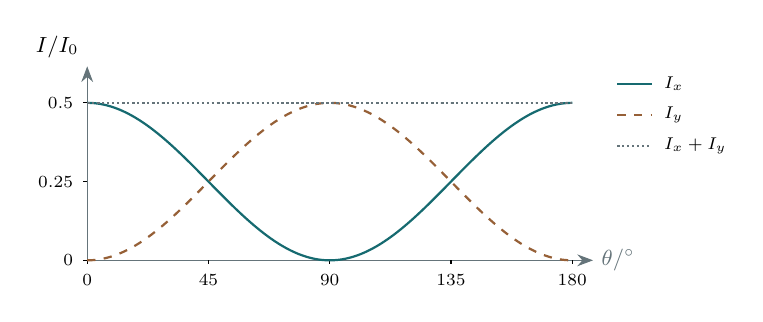
\begin{tikzpicture}[scale=.88,transform shape]
\draw[axis] (0,0.0)--(7.3,0.0) node[right] {$\theta/^\circ$};
\draw[axis] (0,0)--(0,2.8);
\node[above left] at (0,2.8) {$I/I_0$};
\draw[thin] (0.000000,0.0)--(0.000000,-0.06);\node[below,font=\scriptsize] at (0.000000,-0.08) {$ 0 $};
\draw[thin] (1.750000,0.0)--(1.750000,-0.06);\node[below,font=\scriptsize] at (1.750000,-0.08) {$ 45 $};
\draw[thin] (3.500000,0.0)--(3.500000,-0.06);\node[below,font=\scriptsize] at (3.500000,-0.08) {$ 90 $};
\draw[thin] (5.250000,0.0)--(5.250000,-0.06);\node[below,font=\scriptsize] at (5.250000,-0.08) {$ 135 $};
\draw[thin] (7.000000,0.0)--(7.000000,-0.06);\node[below,font=\scriptsize] at (7.000000,-0.08) {$ 180 $};
\draw[thin] (0,0.000000)--(-.06,0.000000);\node[left,font=\scriptsize] at (-.08,0.000000) {$ 0 $};
\draw[thin] (0,1.136364)--(-.06,1.136364);\node[left,font=\scriptsize] at (-.08,1.136364) {$ 0.25 $};
\draw[thin] (0,2.272727)--(-.06,2.272727);\node[left,font=\scriptsize] at (-.08,2.272727) {$ 0.5 $};
\draw[thick,color=accent] plot coordinates {(0.0000000,2.2727273) (0.0291667,2.2723379) (0.0583333,2.2711699) (0.0875000,2.2692242) (0.1166667,2.2665022) (0.1458333,2.2630055) (0.1750000,2.2587368) (0.2041667,2.2536988) (0.2333333,2.2478950) (0.2625000,2.2413295) (0.2916667,2.2340066) (0.3208333,2.2259315) (0.3500000,2.2171097) (0.3791667,2.2075471) (0.4083333,2.1972505) (0.4375000,2.1862267) (0.4666667,2.1744835) (0.4958333,2.1620287) (0.5250000,2.1488711) (0.5541667,2.1350194) (0.5833333,2.1204834) (0.6125000,2.1052729) (0.6416667,2.0893984) (0.6708333,2.0728707) (0.7000000,2.0557011) (0.7291667,2.0379015) (0.7583333,2.0194840) (0.7875000,2.0004613) (0.8166667,1.9808464) (0.8458333,1.9606527) (0.8750000,1.9398941) (0.9041667,1.9185847) (0.9333333,1.8967393) (0.9625000,1.8743728) (0.9916667,1.8515004) (1.0208333,1.8281380) (1.0500000,1.8043014) (1.0791667,1.7800071) (1.1083333,1.7552716) (1.1375000,1.7301120) (1.1666667,1.7045455) (1.1958333,1.6785895) (1.2250000,1.6522619) (1.2541667,1.6255808) (1.2833333,1.5985644) (1.3125000,1.5712312) (1.3416667,1.5435999) (1.3708333,1.5156896) (1.4000000,1.4875193) (1.4291667,1.4591083) (1.4583333,1.4304762) (1.4875000,1.4016425) (1.5166667,1.3726269) (1.5458333,1.3434495) (1.5750000,1.3141301) (1.6041667,1.2846889) (1.6333333,1.2551460) (1.6625000,1.2255217) (1.6916667,1.1958363) (1.7208333,1.1661102) (1.7500000,1.1363636) (1.7791667,1.1066171) (1.8083333,1.0768910) (1.8375000,1.0472056) (1.8666667,1.0175813) (1.8958333,0.9880384) (1.9250000,0.9585972) (1.9541667,0.9292778) (1.9833333,0.9001004) (2.0125000,0.8710848) (2.0416667,0.8422511) (2.0708333,0.8136189) (2.1000000,0.7852080) (2.1291667,0.7570377) (2.1583333,0.7291273) (2.1875000,0.7014961) (2.2166667,0.6741629) (2.2458333,0.6471465) (2.2750000,0.6204653) (2.3041667,0.5941378) (2.3333333,0.5681818) (2.3625000,0.5426153) (2.3916667,0.5174556) (2.4208333,0.4927202) (2.4500000,0.4684258) (2.4791667,0.4445893) (2.5083333,0.4212268) (2.5375000,0.3983545) (2.5666667,0.3759879) (2.5958333,0.3541425) (2.6250000,0.3328332) (2.6541667,0.3120746) (2.6833333,0.2918809) (2.7125000,0.2722659) (2.7416667,0.2532432) (2.7708333,0.2348257) (2.8000000,0.2170261) (2.8291667,0.1998566) (2.8583333,0.1833289) (2.8875000,0.1674544) (2.9166667,0.1522439) (2.9458333,0.1377078) (2.9750000,0.1238562) (3.0041667,0.1106985) (3.0333333,0.0982438) (3.0625000,0.0865005) (3.0916667,0.0754768) (3.1208333,0.0651801) (3.1500000,0.0556176) (3.1791667,0.0467958) (3.2083333,0.0387207) (3.2375000,0.0313978) (3.2666667,0.0248323) (3.2958333,0.0190285) (3.3250000,0.0139905) (3.3541667,0.0097217) (3.3833333,0.0062251) (3.4125000,0.0035030) (3.4416667,0.0015573) (3.4708333,0.0003894) (3.5000000,0.0000000) (3.5291667,0.0003894) (3.5583333,0.0015573) (3.5875000,0.0035030) (3.6166667,0.0062251) (3.6458333,0.0097217) (3.6750000,0.0139905) (3.7041667,0.0190285) (3.7333333,0.0248323) (3.7625000,0.0313978) (3.7916667,0.0387207) (3.8208333,0.0467958) (3.8500000,0.0556176) (3.8791667,0.0651801) (3.9083333,0.0754768) (3.9375000,0.0865005) (3.9666667,0.0982438) (3.9958333,0.1106985) (4.0250000,0.1238562) (4.0541667,0.1377078) (4.0833333,0.1522439) (4.1125000,0.1674544) (4.1416667,0.1833289) (4.1708333,0.1998566) (4.2000000,0.2170261) (4.2291667,0.2348257) (4.2583333,0.2532432) (4.2875000,0.2722659) (4.3166667,0.2918809) (4.3458333,0.3120746) (4.3750000,0.3328332) (4.4041667,0.3541425) (4.4333333,0.3759879) (4.4625000,0.3983545) (4.4916667,0.4212268) (4.5208333,0.4445893) (4.5500000,0.4684258) (4.5791667,0.4927202) (4.6083333,0.5174556) (4.6375000,0.5426153) (4.6666667,0.5681818) (4.6958333,0.5941378) (4.7250000,0.6204653) (4.7541667,0.6471465) (4.7833333,0.6741629) (4.8125000,0.7014961) (4.8416667,0.7291273) (4.8708333,0.7570377) (4.9000000,0.7852080) (4.9291667,0.8136189) (4.9583333,0.8422511) (4.9875000,0.8710848) (5.0166667,0.9001004) (5.0458333,0.9292778) (5.0750000,0.9585972) (5.1041667,0.9880384) (5.1333333,1.0175813) (5.1625000,1.0472056) (5.1916667,1.0768910) (5.2208333,1.1066171) (5.2500000,1.1363636) (5.2791667,1.1661102) (5.3083333,1.1958363) (5.3375000,1.2255217) (5.3666667,1.2551460) (5.3958333,1.2846889) (5.4250000,1.3141301) (5.4541667,1.3434495) (5.4833333,1.3726269) (5.5125000,1.4016425) (5.5416667,1.4304762) (5.5708333,1.4591083) (5.6000000,1.4875193) (5.6291667,1.5156896) (5.6583333,1.5435999) (5.6875000,1.5712312) (5.7166667,1.5985644) (5.7458333,1.6255808) (5.7750000,1.6522619) (5.8041667,1.6785895) (5.8333333,1.7045455) (5.8625000,1.7301120) (5.8916667,1.7552716) (5.9208333,1.7800071) (5.9500000,1.8043014) (5.9791667,1.8281380) (6.0083333,1.8515004) (6.0375000,1.8743728) (6.0666667,1.8967393) (6.0958333,1.9185847) (6.1250000,1.9398941) (6.1541667,1.9606527) (6.1833333,1.9808464) (6.2125000,2.0004613) (6.2416667,2.0194840) (6.2708333,2.0379015) (6.3000000,2.0557011) (6.3291667,2.0728707) (6.3583333,2.0893984) (6.3875000,2.1052729) (6.4166667,2.1204834) (6.4458333,2.1350194) (6.4750000,2.1488711) (6.5041667,2.1620287) (6.5333333,2.1744835) (6.5625000,2.1862267) (6.5916667,2.1972505) (6.6208333,2.2075471) (6.6500000,2.2171097) (6.6791667,2.2259315) (6.7083333,2.2340066) (6.7375000,2.2413295) (6.7666667,2.2478950) (6.7958333,2.2536988) (6.8250000,2.2587368) (6.8541667,2.2630055) (6.8833333,2.2665022) (6.9125000,2.2692242) (6.9416667,2.2711699) (6.9708333,2.2723379) (7.0000000,2.2727273)};
\draw[thick,color=accent] (7.65,2.55)--(8.15,2.55);\node[right,font=\scriptsize] at (8.2,2.55) {$I_x$};
\draw[thick,dashed,color=warm] plot coordinates {(0.0000000,0.0000000) (0.0291667,0.0003894) (0.0583333,0.0015573) (0.0875000,0.0035030) (0.1166667,0.0062251) (0.1458333,0.0097217) (0.1750000,0.0139905) (0.2041667,0.0190285) (0.2333333,0.0248323) (0.2625000,0.0313978) (0.2916667,0.0387207) (0.3208333,0.0467958) (0.3500000,0.0556176) (0.3791667,0.0651801) (0.4083333,0.0754768) (0.4375000,0.0865005) (0.4666667,0.0982438) (0.4958333,0.1106985) (0.5250000,0.1238562) (0.5541667,0.1377078) (0.5833333,0.1522439) (0.6125000,0.1674544) (0.6416667,0.1833289) (0.6708333,0.1998566) (0.7000000,0.2170261) (0.7291667,0.2348257) (0.7583333,0.2532432) (0.7875000,0.2722659) (0.8166667,0.2918809) (0.8458333,0.3120746) (0.8750000,0.3328332) (0.9041667,0.3541425) (0.9333333,0.3759879) (0.9625000,0.3983545) (0.9916667,0.4212268) (1.0208333,0.4445893) (1.0500000,0.4684258) (1.0791667,0.4927202) (1.1083333,0.5174556) (1.1375000,0.5426153) (1.1666667,0.5681818) (1.1958333,0.5941378) (1.2250000,0.6204653) (1.2541667,0.6471465) (1.2833333,0.6741629) (1.3125000,0.7014961) (1.3416667,0.7291273) (1.3708333,0.7570377) (1.4000000,0.7852080) (1.4291667,0.8136189) (1.4583333,0.8422511) (1.4875000,0.8710848) (1.5166667,0.9001004) (1.5458333,0.9292778) (1.5750000,0.9585972) (1.6041667,0.9880384) (1.6333333,1.0175813) (1.6625000,1.0472056) (1.6916667,1.0768910) (1.7208333,1.1066171) (1.7500000,1.1363636) (1.7791667,1.1661102) (1.8083333,1.1958363) (1.8375000,1.2255217) (1.8666667,1.2551460) (1.8958333,1.2846889) (1.9250000,1.3141301) (1.9541667,1.3434495) (1.9833333,1.3726269) (2.0125000,1.4016425) (2.0416667,1.4304762) (2.0708333,1.4591083) (2.1000000,1.4875193) (2.1291667,1.5156896) (2.1583333,1.5435999) (2.1875000,1.5712312) (2.2166667,1.5985644) (2.2458333,1.6255808) (2.2750000,1.6522619) (2.3041667,1.6785895) (2.3333333,1.7045455) (2.3625000,1.7301120) (2.3916667,1.7552716) (2.4208333,1.7800071) (2.4500000,1.8043014) (2.4791667,1.8281380) (2.5083333,1.8515004) (2.5375000,1.8743728) (2.5666667,1.8967393) (2.5958333,1.9185847) (2.6250000,1.9398941) (2.6541667,1.9606527) (2.6833333,1.9808464) (2.7125000,2.0004613) (2.7416667,2.0194840) (2.7708333,2.0379015) (2.8000000,2.0557011) (2.8291667,2.0728707) (2.8583333,2.0893984) (2.8875000,2.1052729) (2.9166667,2.1204834) (2.9458333,2.1350194) (2.9750000,2.1488711) (3.0041667,2.1620287) (3.0333333,2.1744835) (3.0625000,2.1862267) (3.0916667,2.1972505) (3.1208333,2.2075471) (3.1500000,2.2171097) (3.1791667,2.2259315) (3.2083333,2.2340066) (3.2375000,2.2413295) (3.2666667,2.2478950) (3.2958333,2.2536988) (3.3250000,2.2587368) (3.3541667,2.2630055) (3.3833333,2.2665022) (3.4125000,2.2692242) (3.4416667,2.2711699) (3.4708333,2.2723379) (3.5000000,2.2727273) (3.5291667,2.2723379) (3.5583333,2.2711699) (3.5875000,2.2692242) (3.6166667,2.2665022) (3.6458333,2.2630055) (3.6750000,2.2587368) (3.7041667,2.2536988) (3.7333333,2.2478950) (3.7625000,2.2413295) (3.7916667,2.2340066) (3.8208333,2.2259315) (3.8500000,2.2171097) (3.8791667,2.2075471) (3.9083333,2.1972505) (3.9375000,2.1862267) (3.9666667,2.1744835) (3.9958333,2.1620287) (4.0250000,2.1488711) (4.0541667,2.1350194) (4.0833333,2.1204834) (4.1125000,2.1052729) (4.1416667,2.0893984) (4.1708333,2.0728707) (4.2000000,2.0557011) (4.2291667,2.0379015) (4.2583333,2.0194840) (4.2875000,2.0004613) (4.3166667,1.9808464) (4.3458333,1.9606527) (4.3750000,1.9398941) (4.4041667,1.9185847) (4.4333333,1.8967393) (4.4625000,1.8743728) (4.4916667,1.8515004) (4.5208333,1.8281380) (4.5500000,1.8043014) (4.5791667,1.7800071) (4.6083333,1.7552716) (4.6375000,1.7301120) (4.6666667,1.7045455) (4.6958333,1.6785895) (4.7250000,1.6522619) (4.7541667,1.6255808) (4.7833333,1.5985644) (4.8125000,1.5712312) (4.8416667,1.5435999) (4.8708333,1.5156896) (4.9000000,1.4875193) (4.9291667,1.4591083) (4.9583333,1.4304762) (4.9875000,1.4016425) (5.0166667,1.3726269) (5.0458333,1.3434495) (5.0750000,1.3141301) (5.1041667,1.2846889) (5.1333333,1.2551460) (5.1625000,1.2255217) (5.1916667,1.1958363) (5.2208333,1.1661102) (5.2500000,1.1363636) (5.2791667,1.1066171) (5.3083333,1.0768910) (5.3375000,1.0472056) (5.3666667,1.0175813) (5.3958333,0.9880384) (5.4250000,0.9585972) (5.4541667,0.9292778) (5.4833333,0.9001004) (5.5125000,0.8710848) (5.5416667,0.8422511) (5.5708333,0.8136189) (5.6000000,0.7852080) (5.6291667,0.7570377) (5.6583333,0.7291273) (5.6875000,0.7014961) (5.7166667,0.6741629) (5.7458333,0.6471465) (5.7750000,0.6204653) (5.8041667,0.5941378) (5.8333333,0.5681818) (5.8625000,0.5426153) (5.8916667,0.5174556) (5.9208333,0.4927202) (5.9500000,0.4684258) (5.9791667,0.4445893) (6.0083333,0.4212268) (6.0375000,0.3983545) (6.0666667,0.3759879) (6.0958333,0.3541425) (6.1250000,0.3328332) (6.1541667,0.3120746) (6.1833333,0.2918809) (6.2125000,0.2722659) (6.2416667,0.2532432) (6.2708333,0.2348257) (6.3000000,0.2170261) (6.3291667,0.1998566) (6.3583333,0.1833289) (6.3875000,0.1674544) (6.4166667,0.1522439) (6.4458333,0.1377078) (6.4750000,0.1238562) (6.5041667,0.1106985) (6.5333333,0.0982438) (6.5625000,0.0865005) (6.5916667,0.0754768) (6.6208333,0.0651801) (6.6500000,0.0556176) (6.6791667,0.0467958) (6.7083333,0.0387207) (6.7375000,0.0313978) (6.7666667,0.0248323) (6.7958333,0.0190285) (6.8250000,0.0139905) (6.8541667,0.0097217) (6.8833333,0.0062251) (6.9125000,0.0035030) (6.9416667,0.0015573) (6.9708333,0.0003894) (7.0000000,0.0000000)};
\draw[thick,dashed,color=warm] (7.65,2.0999999999999996)--(8.15,2.0999999999999996);\node[right,font=\scriptsize] at (8.2,2.0999999999999996) {$I_y$};
\draw[densely dotted,thick,color=muted] plot coordinates {(0.0000000,2.2727273) (0.0291667,2.2727273) (0.0583333,2.2727273) (0.0875000,2.2727273) (0.1166667,2.2727273) (0.1458333,2.2727273) (0.1750000,2.2727273) (0.2041667,2.2727273) (0.2333333,2.2727273) (0.2625000,2.2727273) (0.2916667,2.2727273) (0.3208333,2.2727273) (0.3500000,2.2727273) (0.3791667,2.2727273) (0.4083333,2.2727273) (0.4375000,2.2727273) (0.4666667,2.2727273) (0.4958333,2.2727273) (0.5250000,2.2727273) (0.5541667,2.2727273) (0.5833333,2.2727273) (0.6125000,2.2727273) (0.6416667,2.2727273) (0.6708333,2.2727273) (0.7000000,2.2727273) (0.7291667,2.2727273) (0.7583333,2.2727273) (0.7875000,2.2727273) (0.8166667,2.2727273) (0.8458333,2.2727273) (0.8750000,2.2727273) (0.9041667,2.2727273) (0.9333333,2.2727273) (0.9625000,2.2727273) (0.9916667,2.2727273) (1.0208333,2.2727273) (1.0500000,2.2727273) (1.0791667,2.2727273) (1.1083333,2.2727273) (1.1375000,2.2727273) (1.1666667,2.2727273) (1.1958333,2.2727273) (1.2250000,2.2727273) (1.2541667,2.2727273) (1.2833333,2.2727273) (1.3125000,2.2727273) (1.3416667,2.2727273) (1.3708333,2.2727273) (1.4000000,2.2727273) (1.4291667,2.2727273) (1.4583333,2.2727273) (1.4875000,2.2727273) (1.5166667,2.2727273) (1.5458333,2.2727273) (1.5750000,2.2727273) (1.6041667,2.2727273) (1.6333333,2.2727273) (1.6625000,2.2727273) (1.6916667,2.2727273) (1.7208333,2.2727273) (1.7500000,2.2727273) (1.7791667,2.2727273) (1.8083333,2.2727273) (1.8375000,2.2727273) (1.8666667,2.2727273) (1.8958333,2.2727273) (1.9250000,2.2727273) (1.9541667,2.2727273) (1.9833333,2.2727273) (2.0125000,2.2727273) (2.0416667,2.2727273) (2.0708333,2.2727273) (2.1000000,2.2727273) (2.1291667,2.2727273) (2.1583333,2.2727273) (2.1875000,2.2727273) (2.2166667,2.2727273) (2.2458333,2.2727273) (2.2750000,2.2727273) (2.3041667,2.2727273) (2.3333333,2.2727273) (2.3625000,2.2727273) (2.3916667,2.2727273) (2.4208333,2.2727273) (2.4500000,2.2727273) (2.4791667,2.2727273) (2.5083333,2.2727273) (2.5375000,2.2727273) (2.5666667,2.2727273) (2.5958333,2.2727273) (2.6250000,2.2727273) (2.6541667,2.2727273) (2.6833333,2.2727273) (2.7125000,2.2727273) (2.7416667,2.2727273) (2.7708333,2.2727273) (2.8000000,2.2727273) (2.8291667,2.2727273) (2.8583333,2.2727273) (2.8875000,2.2727273) (2.9166667,2.2727273) (2.9458333,2.2727273) (2.9750000,2.2727273) (3.0041667,2.2727273) (3.0333333,2.2727273) (3.0625000,2.2727273) (3.0916667,2.2727273) (3.1208333,2.2727273) (3.1500000,2.2727273) (3.1791667,2.2727273) (3.2083333,2.2727273) (3.2375000,2.2727273) (3.2666667,2.2727273) (3.2958333,2.2727273) (3.3250000,2.2727273) (3.3541667,2.2727273) (3.3833333,2.2727273) (3.4125000,2.2727273) (3.4416667,2.2727273) (3.4708333,2.2727273) (3.5000000,2.2727273) (3.5291667,2.2727273) (3.5583333,2.2727273) (3.5875000,2.2727273) (3.6166667,2.2727273) (3.6458333,2.2727273) (3.6750000,2.2727273) (3.7041667,2.2727273) (3.7333333,2.2727273) (3.7625000,2.2727273) (3.7916667,2.2727273) (3.8208333,2.2727273) (3.8500000,2.2727273) (3.8791667,2.2727273) (3.9083333,2.2727273) (3.9375000,2.2727273) (3.9666667,2.2727273) (3.9958333,2.2727273) (4.0250000,2.2727273) (4.0541667,2.2727273) (4.0833333,2.2727273) (4.1125000,2.2727273) (4.1416667,2.2727273) (4.1708333,2.2727273) (4.2000000,2.2727273) (4.2291667,2.2727273) (4.2583333,2.2727273) (4.2875000,2.2727273) (4.3166667,2.2727273) (4.3458333,2.2727273) (4.3750000,2.2727273) (4.4041667,2.2727273) (4.4333333,2.2727273) (4.4625000,2.2727273) (4.4916667,2.2727273) (4.5208333,2.2727273) (4.5500000,2.2727273) (4.5791667,2.2727273) (4.6083333,2.2727273) (4.6375000,2.2727273) (4.6666667,2.2727273) (4.6958333,2.2727273) (4.7250000,2.2727273) (4.7541667,2.2727273) (4.7833333,2.2727273) (4.8125000,2.2727273) (4.8416667,2.2727273) (4.8708333,2.2727273) (4.9000000,2.2727273) (4.9291667,2.2727273) (4.9583333,2.2727273) (4.9875000,2.2727273) (5.0166667,2.2727273) (5.0458333,2.2727273) (5.0750000,2.2727273) (5.1041667,2.2727273) (5.1333333,2.2727273) (5.1625000,2.2727273) (5.1916667,2.2727273) (5.2208333,2.2727273) (5.2500000,2.2727273) (5.2791667,2.2727273) (5.3083333,2.2727273) (5.3375000,2.2727273) (5.3666667,2.2727273) (5.3958333,2.2727273) (5.4250000,2.2727273) (5.4541667,2.2727273) (5.4833333,2.2727273) (5.5125000,2.2727273) (5.5416667,2.2727273) (5.5708333,2.2727273) (5.6000000,2.2727273) (5.6291667,2.2727273) (5.6583333,2.2727273) (5.6875000,2.2727273) (5.7166667,2.2727273) (5.7458333,2.2727273) (5.7750000,2.2727273) (5.8041667,2.2727273) (5.8333333,2.2727273) (5.8625000,2.2727273) (5.8916667,2.2727273) (5.9208333,2.2727273) (5.9500000,2.2727273) (5.9791667,2.2727273) (6.0083333,2.2727273) (6.0375000,2.2727273) (6.0666667,2.2727273) (6.0958333,2.2727273) (6.1250000,2.2727273) (6.1541667,2.2727273) (6.1833333,2.2727273) (6.2125000,2.2727273) (6.2416667,2.2727273) (6.2708333,2.2727273) (6.3000000,2.2727273) (6.3291667,2.2727273) (6.3583333,2.2727273) (6.3875000,2.2727273) (6.4166667,2.2727273) (6.4458333,2.2727273) (6.4750000,2.2727273) (6.5041667,2.2727273) (6.5333333,2.2727273) (6.5625000,2.2727273) (6.5916667,2.2727273) (6.6208333,2.2727273) (6.6500000,2.2727273) (6.6791667,2.2727273) (6.7083333,2.2727273) (6.7375000,2.2727273) (6.7666667,2.2727273) (6.7958333,2.2727273) (6.8250000,2.2727273) (6.8541667,2.2727273) (6.8833333,2.2727273) (6.9125000,2.2727273) (6.9416667,2.2727273) (6.9708333,2.2727273) (7.0000000,2.2727273)};
\draw[densely dotted,thick,color=muted] (7.65,1.65)--(8.15,1.65);\node[right,font=\scriptsize] at (8.2,1.65) {$I_x+I_y$};
\end{tikzpicture}
\figcaption{解图光4.1B\quad 两正交等强不相干分量的投影强度相加}
\end{minipage}\end{center}

理想片的场投影算符为$\mathsf P=\boldsymbol p\boldsymbol p^\mathsf T$，输出统计矩阵为
\[
\mathsf J_{\rm out}=\mathsf P\mathsf J_{\rm in}\mathsf P
=\frac{I_0}{2}\mathsf P,\qquad
\operatorname{tr}\mathsf J_{\rm out}=\frac{I_0}{2},\quad
\det\mathsf J_{\rm out}=0.
\]
矩阵只有一个非零本征值，所以输出完全线偏振。继续放一片同轴理想偏振片，$\mathsf P^2=\mathsf P$，输出不再减半；转过$\beta$才再乘$\cos^2\beta$。半强说明总功率，完全偏振说明场方向的相关性；两者描述不同的量。

\textbf{检偏强度与入射统计矩阵。}对一般入射矩阵，
\[
I(\theta)=\frac{J_{xx}+J_{yy}}2+
\frac{J_{xx}-J_{yy}}2\cos2\theta+
\operatorname{Re}J_{xy}\sin2\theta.
\]
线检偏强度随角度保持常量的条件是 $J_{xx}=J_{yy}$、$\operatorname{Re}J_{xy}=0$，透过量为总强度的一半。自然光还有 $\operatorname{Im}J_{xy}=0$；圆偏振的两个等强分量相差 $\pi/2$，故互相关有虚部。图C中，两个正交分量强度不相等时，检偏轴向较强分量转去，读数便升高。要区分同样给出恒定半强的自然光与圆偏振，可以让两束分别先通过四分之一波片。在该片的两条轴上取矩阵 $\operatorname{diag}(1,i)$，圆偏态 $(1,\pm i)^T/\sqrt2$ 变为线偏态 $(1,\mp1)^T/\sqrt2$，随后检偏器的读数随角度作马吕斯变化。自然光的矩阵在无损波片作用下仍与单位矩阵成正比，继续给恒定半强。

\begin{center}\begin{minipage}{.98\linewidth}\centering
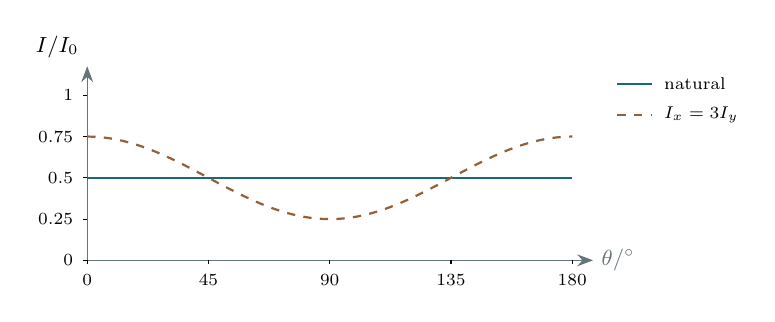
\begin{tikzpicture}[scale=.88,transform shape]
\draw[axis] (0,0.0)--(7.3,0.0) node[right] {$\theta/^\circ$};
\draw[axis] (0,0)--(0,2.8);
\node[above left] at (0,2.8) {$I/I_0$};
\draw[thin] (0.000000,0.0)--(0.000000,-0.06);\node[below,font=\scriptsize] at (0.000000,-0.08) {$ 0 $};
\draw[thin] (1.750000,0.0)--(1.750000,-0.06);\node[below,font=\scriptsize] at (1.750000,-0.08) {$ 45 $};
\draw[thin] (3.500000,0.0)--(3.500000,-0.06);\node[below,font=\scriptsize] at (3.500000,-0.08) {$ 90 $};
\draw[thin] (5.250000,0.0)--(5.250000,-0.06);\node[below,font=\scriptsize] at (5.250000,-0.08) {$ 135 $};
\draw[thin] (7.000000,0.0)--(7.000000,-0.06);\node[below,font=\scriptsize] at (7.000000,-0.08) {$ 180 $};
\draw[thin] (0,0.000000)--(-.06,0.000000);\node[left,font=\scriptsize] at (-.08,0.000000) {$ 0 $};
\draw[thin] (0,0.595238)--(-.06,0.595238);\node[left,font=\scriptsize] at (-.08,0.595238) {$ 0.25 $};
\draw[thin] (0,1.190476)--(-.06,1.190476);\node[left,font=\scriptsize] at (-.08,1.190476) {$ 0.5 $};
\draw[thin] (0,1.785714)--(-.06,1.785714);\node[left,font=\scriptsize] at (-.08,1.785714) {$ 0.75 $};
\draw[thin] (0,2.380952)--(-.06,2.380952);\node[left,font=\scriptsize] at (-.08,2.380952) {$ 1 $};
\draw[thick,color=accent] plot coordinates {(0.0000000,1.1904762) (0.0291667,1.1904762) (0.0583333,1.1904762) (0.0875000,1.1904762) (0.1166667,1.1904762) (0.1458333,1.1904762) (0.1750000,1.1904762) (0.2041667,1.1904762) (0.2333333,1.1904762) (0.2625000,1.1904762) (0.2916667,1.1904762) (0.3208333,1.1904762) (0.3500000,1.1904762) (0.3791667,1.1904762) (0.4083333,1.1904762) (0.4375000,1.1904762) (0.4666667,1.1904762) (0.4958333,1.1904762) (0.5250000,1.1904762) (0.5541667,1.1904762) (0.5833333,1.1904762) (0.6125000,1.1904762) (0.6416667,1.1904762) (0.6708333,1.1904762) (0.7000000,1.1904762) (0.7291667,1.1904762) (0.7583333,1.1904762) (0.7875000,1.1904762) (0.8166667,1.1904762) (0.8458333,1.1904762) (0.8750000,1.1904762) (0.9041667,1.1904762) (0.9333333,1.1904762) (0.9625000,1.1904762) (0.9916667,1.1904762) (1.0208333,1.1904762) (1.0500000,1.1904762) (1.0791667,1.1904762) (1.1083333,1.1904762) (1.1375000,1.1904762) (1.1666667,1.1904762) (1.1958333,1.1904762) (1.2250000,1.1904762) (1.2541667,1.1904762) (1.2833333,1.1904762) (1.3125000,1.1904762) (1.3416667,1.1904762) (1.3708333,1.1904762) (1.4000000,1.1904762) (1.4291667,1.1904762) (1.4583333,1.1904762) (1.4875000,1.1904762) (1.5166667,1.1904762) (1.5458333,1.1904762) (1.5750000,1.1904762) (1.6041667,1.1904762) (1.6333333,1.1904762) (1.6625000,1.1904762) (1.6916667,1.1904762) (1.7208333,1.1904762) (1.7500000,1.1904762) (1.7791667,1.1904762) (1.8083333,1.1904762) (1.8375000,1.1904762) (1.8666667,1.1904762) (1.8958333,1.1904762) (1.9250000,1.1904762) (1.9541667,1.1904762) (1.9833333,1.1904762) (2.0125000,1.1904762) (2.0416667,1.1904762) (2.0708333,1.1904762) (2.1000000,1.1904762) (2.1291667,1.1904762) (2.1583333,1.1904762) (2.1875000,1.1904762) (2.2166667,1.1904762) (2.2458333,1.1904762) (2.2750000,1.1904762) (2.3041667,1.1904762) (2.3333333,1.1904762) (2.3625000,1.1904762) (2.3916667,1.1904762) (2.4208333,1.1904762) (2.4500000,1.1904762) (2.4791667,1.1904762) (2.5083333,1.1904762) (2.5375000,1.1904762) (2.5666667,1.1904762) (2.5958333,1.1904762) (2.6250000,1.1904762) (2.6541667,1.1904762) (2.6833333,1.1904762) (2.7125000,1.1904762) (2.7416667,1.1904762) (2.7708333,1.1904762) (2.8000000,1.1904762) (2.8291667,1.1904762) (2.8583333,1.1904762) (2.8875000,1.1904762) (2.9166667,1.1904762) (2.9458333,1.1904762) (2.9750000,1.1904762) (3.0041667,1.1904762) (3.0333333,1.1904762) (3.0625000,1.1904762) (3.0916667,1.1904762) (3.1208333,1.1904762) (3.1500000,1.1904762) (3.1791667,1.1904762) (3.2083333,1.1904762) (3.2375000,1.1904762) (3.2666667,1.1904762) (3.2958333,1.1904762) (3.3250000,1.1904762) (3.3541667,1.1904762) (3.3833333,1.1904762) (3.4125000,1.1904762) (3.4416667,1.1904762) (3.4708333,1.1904762) (3.5000000,1.1904762) (3.5291667,1.1904762) (3.5583333,1.1904762) (3.5875000,1.1904762) (3.6166667,1.1904762) (3.6458333,1.1904762) (3.6750000,1.1904762) (3.7041667,1.1904762) (3.7333333,1.1904762) (3.7625000,1.1904762) (3.7916667,1.1904762) (3.8208333,1.1904762) (3.8500000,1.1904762) (3.8791667,1.1904762) (3.9083333,1.1904762) (3.9375000,1.1904762) (3.9666667,1.1904762) (3.9958333,1.1904762) (4.0250000,1.1904762) (4.0541667,1.1904762) (4.0833333,1.1904762) (4.1125000,1.1904762) (4.1416667,1.1904762) (4.1708333,1.1904762) (4.2000000,1.1904762) (4.2291667,1.1904762) (4.2583333,1.1904762) (4.2875000,1.1904762) (4.3166667,1.1904762) (4.3458333,1.1904762) (4.3750000,1.1904762) (4.4041667,1.1904762) (4.4333333,1.1904762) (4.4625000,1.1904762) (4.4916667,1.1904762) (4.5208333,1.1904762) (4.5500000,1.1904762) (4.5791667,1.1904762) (4.6083333,1.1904762) (4.6375000,1.1904762) (4.6666667,1.1904762) (4.6958333,1.1904762) (4.7250000,1.1904762) (4.7541667,1.1904762) (4.7833333,1.1904762) (4.8125000,1.1904762) (4.8416667,1.1904762) (4.8708333,1.1904762) (4.9000000,1.1904762) (4.9291667,1.1904762) (4.9583333,1.1904762) (4.9875000,1.1904762) (5.0166667,1.1904762) (5.0458333,1.1904762) (5.0750000,1.1904762) (5.1041667,1.1904762) (5.1333333,1.1904762) (5.1625000,1.1904762) (5.1916667,1.1904762) (5.2208333,1.1904762) (5.2500000,1.1904762) (5.2791667,1.1904762) (5.3083333,1.1904762) (5.3375000,1.1904762) (5.3666667,1.1904762) (5.3958333,1.1904762) (5.4250000,1.1904762) (5.4541667,1.1904762) (5.4833333,1.1904762) (5.5125000,1.1904762) (5.5416667,1.1904762) (5.5708333,1.1904762) (5.6000000,1.1904762) (5.6291667,1.1904762) (5.6583333,1.1904762) (5.6875000,1.1904762) (5.7166667,1.1904762) (5.7458333,1.1904762) (5.7750000,1.1904762) (5.8041667,1.1904762) (5.8333333,1.1904762) (5.8625000,1.1904762) (5.8916667,1.1904762) (5.9208333,1.1904762) (5.9500000,1.1904762) (5.9791667,1.1904762) (6.0083333,1.1904762) (6.0375000,1.1904762) (6.0666667,1.1904762) (6.0958333,1.1904762) (6.1250000,1.1904762) (6.1541667,1.1904762) (6.1833333,1.1904762) (6.2125000,1.1904762) (6.2416667,1.1904762) (6.2708333,1.1904762) (6.3000000,1.1904762) (6.3291667,1.1904762) (6.3583333,1.1904762) (6.3875000,1.1904762) (6.4166667,1.1904762) (6.4458333,1.1904762) (6.4750000,1.1904762) (6.5041667,1.1904762) (6.5333333,1.1904762) (6.5625000,1.1904762) (6.5916667,1.1904762) (6.6208333,1.1904762) (6.6500000,1.1904762) (6.6791667,1.1904762) (6.7083333,1.1904762) (6.7375000,1.1904762) (6.7666667,1.1904762) (6.7958333,1.1904762) (6.8250000,1.1904762) (6.8541667,1.1904762) (6.8833333,1.1904762) (6.9125000,1.1904762) (6.9416667,1.1904762) (6.9708333,1.1904762) (7.0000000,1.1904762)};
\draw[thick,color=accent] (7.65,2.55)--(8.15,2.55);\node[right,font=\scriptsize] at (8.2,2.55) {$\mathrm{natural}$};
\draw[thick,dashed,color=warm] plot coordinates {(0.0000000,1.7857143) (0.0291667,1.7855103) (0.0583333,1.7848985) (0.0875000,1.7838794) (0.1166667,1.7824535) (0.1458333,1.7806219) (0.1750000,1.7783859) (0.2041667,1.7757470) (0.2333333,1.7727069) (0.2625000,1.7692678) (0.2916667,1.7654320) (0.3208333,1.7612022) (0.3500000,1.7565813) (0.3791667,1.7515723) (0.4083333,1.7461788) (0.4375000,1.7404045) (0.4666667,1.7342532) (0.4958333,1.7277293) (0.5250000,1.7208372) (0.5541667,1.7135816) (0.5833333,1.7059675) (0.6125000,1.6980001) (0.6416667,1.6896849) (0.6708333,1.6810275) (0.7000000,1.6720339) (0.7291667,1.6627103) (0.7583333,1.6530631) (0.7875000,1.6430988) (0.8166667,1.6328243) (0.8458333,1.6222466) (0.8750000,1.6113731) (0.9041667,1.6002111) (0.9333333,1.5887682) (0.9625000,1.5770524) (0.9916667,1.5650717) (1.0208333,1.5528342) (1.0500000,1.5403484) (1.0791667,1.5276228) (1.1083333,1.5146661) (1.1375000,1.5014872) (1.1666667,1.4880952) (1.1958333,1.4744993) (1.2250000,1.4607086) (1.2541667,1.4467328) (1.2833333,1.4325813) (1.3125000,1.4182639) (1.3416667,1.4037904) (1.3708333,1.3891707) (1.4000000,1.3744149) (1.4291667,1.3595329) (1.4583333,1.3445351) (1.4875000,1.3294318) (1.5166667,1.3142331) (1.5458333,1.2989497) (1.5750000,1.2835919) (1.6041667,1.2681704) (1.6333333,1.2526955) (1.6625000,1.2371780) (1.6916667,1.2216285) (1.7208333,1.2060577) (1.7500000,1.1904762) (1.7791667,1.1748947) (1.8083333,1.1593238) (1.8375000,1.1437743) (1.8666667,1.1282569) (1.8958333,1.1127820) (1.9250000,1.0973604) (1.9541667,1.0820027) (1.9833333,1.0667192) (2.0125000,1.0515206) (2.0416667,1.0364172) (2.0708333,1.0214194) (2.1000000,1.0065375) (2.1291667,0.9917816) (2.1583333,0.9771619) (2.1875000,0.9626884) (2.2166667,0.9483710) (2.2458333,0.9342196) (2.2750000,0.9202438) (2.3041667,0.9064531) (2.3333333,0.8928571) (2.3625000,0.8794651) (2.3916667,0.8662863) (2.4208333,0.8533296) (2.4500000,0.8406040) (2.4791667,0.8281182) (2.5083333,0.8158807) (2.5375000,0.8039000) (2.5666667,0.7921842) (2.5958333,0.7807413) (2.6250000,0.7695793) (2.6541667,0.7587057) (2.6833333,0.7481281) (2.7125000,0.7378536) (2.7416667,0.7278893) (2.7708333,0.7182421) (2.8000000,0.7089185) (2.8291667,0.6999249) (2.8583333,0.6912675) (2.8875000,0.6829523) (2.9166667,0.6749849) (2.9458333,0.6673708) (2.9750000,0.6601152) (3.0041667,0.6532230) (3.0333333,0.6466991) (3.0625000,0.6405479) (3.0916667,0.6347736) (3.1208333,0.6293801) (3.1500000,0.6243711) (3.1791667,0.6197502) (3.2083333,0.6155203) (3.2375000,0.6116846) (3.2666667,0.6082455) (3.2958333,0.6052054) (3.3250000,0.6025665) (3.3541667,0.6003304) (3.3833333,0.5984989) (3.4125000,0.5970730) (3.4416667,0.5960538) (3.4708333,0.5954421) (3.5000000,0.5952381) (3.5291667,0.5954421) (3.5583333,0.5960538) (3.5875000,0.5970730) (3.6166667,0.5984989) (3.6458333,0.6003304) (3.6750000,0.6025665) (3.7041667,0.6052054) (3.7333333,0.6082455) (3.7625000,0.6116846) (3.7916667,0.6155203) (3.8208333,0.6197502) (3.8500000,0.6243711) (3.8791667,0.6293801) (3.9083333,0.6347736) (3.9375000,0.6405479) (3.9666667,0.6466991) (3.9958333,0.6532230) (4.0250000,0.6601152) (4.0541667,0.6673708) (4.0833333,0.6749849) (4.1125000,0.6829523) (4.1416667,0.6912675) (4.1708333,0.6999249) (4.2000000,0.7089185) (4.2291667,0.7182421) (4.2583333,0.7278893) (4.2875000,0.7378536) (4.3166667,0.7481281) (4.3458333,0.7587057) (4.3750000,0.7695793) (4.4041667,0.7807413) (4.4333333,0.7921842) (4.4625000,0.8039000) (4.4916667,0.8158807) (4.5208333,0.8281182) (4.5500000,0.8406040) (4.5791667,0.8533296) (4.6083333,0.8662863) (4.6375000,0.8794651) (4.6666667,0.8928571) (4.6958333,0.9064531) (4.7250000,0.9202438) (4.7541667,0.9342196) (4.7833333,0.9483710) (4.8125000,0.9626884) (4.8416667,0.9771619) (4.8708333,0.9917816) (4.9000000,1.0065375) (4.9291667,1.0214194) (4.9583333,1.0364172) (4.9875000,1.0515206) (5.0166667,1.0667192) (5.0458333,1.0820027) (5.0750000,1.0973604) (5.1041667,1.1127820) (5.1333333,1.1282569) (5.1625000,1.1437743) (5.1916667,1.1593238) (5.2208333,1.1748947) (5.2500000,1.1904762) (5.2791667,1.2060577) (5.3083333,1.2216285) (5.3375000,1.2371780) (5.3666667,1.2526955) (5.3958333,1.2681704) (5.4250000,1.2835919) (5.4541667,1.2989497) (5.4833333,1.3142331) (5.5125000,1.3294318) (5.5416667,1.3445351) (5.5708333,1.3595329) (5.6000000,1.3744149) (5.6291667,1.3891707) (5.6583333,1.4037904) (5.6875000,1.4182639) (5.7166667,1.4325813) (5.7458333,1.4467328) (5.7750000,1.4607086) (5.8041667,1.4744993) (5.8333333,1.4880952) (5.8625000,1.5014872) (5.8916667,1.5146661) (5.9208333,1.5276228) (5.9500000,1.5403484) (5.9791667,1.5528342) (6.0083333,1.5650717) (6.0375000,1.5770524) (6.0666667,1.5887682) (6.0958333,1.6002111) (6.1250000,1.6113731) (6.1541667,1.6222466) (6.1833333,1.6328243) (6.2125000,1.6430988) (6.2416667,1.6530631) (6.2708333,1.6627103) (6.3000000,1.6720339) (6.3291667,1.6810275) (6.3583333,1.6896849) (6.3875000,1.6980001) (6.4166667,1.7059675) (6.4458333,1.7135816) (6.4750000,1.7208372) (6.5041667,1.7277293) (6.5333333,1.7342532) (6.5625000,1.7404045) (6.5916667,1.7461788) (6.6208333,1.7515723) (6.6500000,1.7565813) (6.6791667,1.7612022) (6.7083333,1.7654320) (6.7375000,1.7692678) (6.7666667,1.7727069) (6.7958333,1.7757470) (6.8250000,1.7783859) (6.8541667,1.7806219) (6.8833333,1.7824535) (6.9125000,1.7838794) (6.9416667,1.7848985) (6.9708333,1.7855103) (7.0000000,1.7857143)};
\draw[thick,dashed,color=warm] (7.65,2.0999999999999996)--(8.15,2.0999999999999996);\node[right,font=\scriptsize] at (8.2,2.0999999999999996) {$I_x=3I_y$};
\end{tikzpicture}
\figcaption{解图光4.1C\quad 等总强度但不同正交统计的旋转检偏曲线}
\end{minipage}\end{center}

\textbf{角向权重、能量与非理想透射。}若用整周$0\le\alpha<2\pi$标方向，权重应改为$I_0/(2\pi)$；同一无向线轴虽出现两次，但每份权重相应减半，积分仍是$I_0/2$。不能只改积分上限而不改归一化。两正交输出端的强度满足
\[
I_{\boldsymbol p}=\frac{I_0}{2},\qquad
I_{\boldsymbol p_\perp}=\frac{I_0}{2},\qquad
I_{\boldsymbol p}+I_{\boldsymbol p_\perp}=I_0.
\]
图D把通过轴与被拒绝正交轴的两份功率分开；它表示理想选择的功率分配，不要求所有实际偏振片都有两个可用出射端。

\begin{center}\begin{minipage}{.98\linewidth}\centering
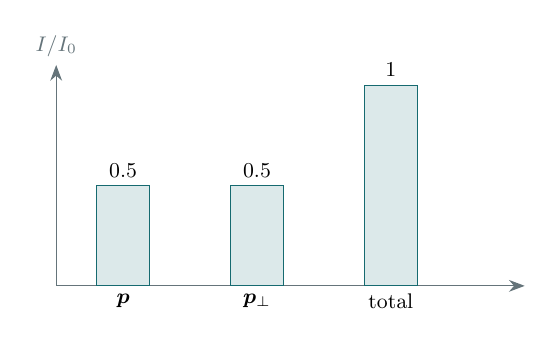
\begin{tikzpicture}[scale=.85,transform shape]
\draw[axis] (0,0)--(7,0); \draw[axis] (0,0)--(0,3.3) node[above] {$I/I_0$};
\filldraw[fill=accent!15,draw=accent] (0.6,0) rectangle (1.4,1.5); \node[above] at (1,1.5) {$ 0.5 $}; \node[below] at (1,0) {$\boldsymbol p$};
\filldraw[fill=accent!15,draw=accent] (2.6,0) rectangle (3.4,1.5); \node[above] at (3,1.5) {$ 0.5 $}; \node[below] at (3,0) {$\boldsymbol p_\perp$};
\filldraw[fill=accent!15,draw=accent] (4.6,0) rectangle (5.4,3); \node[above] at (5,3) {$ 1 $}; \node[below] at (5,0) {$\mathrm{total}$};
\end{tikzpicture}
\figcaption{解图光4.1D\quad 选中与被拒绝正交偏振的功率，总量恢复入射值}
\end{minipage}\end{center}

若两本征轴的强度透过率分别为$T_\parallel,T_\perp$，输出总强度是$I_0(T_\parallel+T_\perp)/2$，自然光入射时仍不随器件方位改变。只有$T_\perp=0$且$T_\parallel>0$时，单端输出才完全线偏振；若两者相等，则只是无偏振选择的衰减片。把某一透过率写成振幅系数时必须取平方根，不能把强度透过率直接乘在电场上。


\Needspace{13\baselineskip}

\pdfbookmark[2]{第 2 题 旋转检偏器与部分偏振光}{q2}

\section*{第 2 题\quad 旋转检偏器与部分偏振光}\label{q:2}

任意一束部分偏振光通过理想线检偏器，转动检偏器一周。求透射强度随方位角的通式，说明最大、最小透射方向的关系，并证明：就线检偏器的透射结果而言，该光束可等效为自然光与线偏振光的叠加。讨论透射强度与角度无关的情况。

\begin{center}\begin{minipage}{.98\linewidth}\centering
\begin{tikzpicture}[scale=.9,transform shape]
\draw[motion] (-1.00000,0.00000)--(1.00000,0.00000);\draw[object] (-0.12000,-0.80000)--(0.12000,-0.80000)--(0.12000,0.80000)--(-0.12000,0.80000)--(-0.12000,-0.80000);\node[above] at (0.00000,1.00000) {检偏器};\node[below] at (0.00000,-1.05000) {$\theta$};\begin{scope}[shift={(4.00000,0.00000)}]
\draw[axis] (-1.60000,0.00000)--(1.60000,0.00000);\draw[axis] (0.00000,-1.60000)--(0.00000,1.60000);\node[below right] at (1.60000,0.00000) {$x$};\node[above right] at (0.00000,1.60000) {$y$};\draw[force] (-1.22873,-0.86036)--(1.22873,0.86036);\node[above right] at (1.33522,0.93493) {$\theta$};
\end{scope}
\end{tikzpicture}
\figcaption{图光4.2\quad 检偏器角度相对于固定入射横轴定义}
\end{minipage}\end{center}

\Needspace{6\baselineskip}\subsection*{解答}


\textbf{固定入射统计量。}检偏片旋转时，入射光的状态保持不变；以下$I(\theta)$是时间平均透射强度。连续线方向分布只是可以采用的一种统计表示，讨论任意部分偏振光时还应允许椭圆偏振和互相关。输出曲线的全部系数先由入射场求出，再对$\theta$求极值，不把随$\theta$变化的积分中值方向当成固定物理轴。

在图光4.2的横截面上，令检偏轴对$x$的角度为$\theta$。先用互不相干的线偏振方向分量说明角度依赖：若其强度权重为$w(\alpha)\dd\alpha$，则
\[
I(\theta)=\int_0^\pi w(\alpha)\cos^2(\alpha-\theta)\dd\alpha.
\]
展开二倍角后，定义与检偏角无关的三个积分
\[
S_0=\int_0^\pi w\dd\alpha,\quad
S_1=\int_0^\pi w\cos2\alpha\dd\alpha,\quad
S_2=\int_0^\pi w\sin2\alpha\dd\alpha,
\]
得到$I(\theta)=[S_0+S_1\cos2\theta+S_2\sin2\theta]/2$。椭圆偏振和部分相干光同样适用：展开$\langle|E_x\cos\theta+E_y\sin\theta|^2\rangle$即可，其中$S_0=\langle|E_x|^2+|E_y|^2\rangle$、$S_1=\langle|E_x|^2-|E_y|^2\rangle$、$S_2=2\operatorname{Re}\langle E_xE_y^*\rangle$。
\begin{center}\begin{minipage}{.98\linewidth}\centering
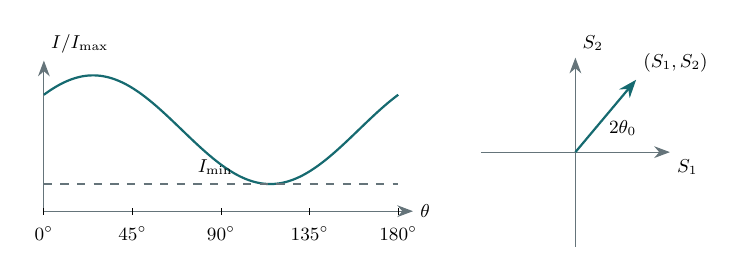
\begin{tikzpicture}[scale=.75,transform shape]
\draw[axis] (0.00000,0.00000)--(6.25000,0.00000);\draw[axis] (0.00000,0.00000)--(0.00000,2.55000);\node[right] at (6.25000,0.00000) {$\theta$};\node[above right] at (0.00000,2.55000) {$I/I_{\max}$};\draw[traj] plot coordinates {(0.00000,1.97136) (0.01200,1.98017) (0.02400,1.98889) (0.03600,1.99751) (0.04800,2.00603) (0.06000,2.01445) (0.07200,2.02277) (0.08400,2.03099) (0.09600,2.03911) (0.10800,2.04712) (0.12000,2.05503) (0.13200,2.06283) (0.14400,2.07053) (0.15600,2.07811) (0.16800,2.08559) (0.18000,2.09295) (0.19200,2.10020) (0.20400,2.10734) (0.21600,2.11436) (0.22800,2.12126) (0.24000,2.12805) (0.25200,2.13472) (0.26400,2.14127) (0.27600,2.14771) (0.28800,2.15402) (0.30000,2.16020) (0.31200,2.16627) (0.32400,2.17221) (0.33600,2.17802) (0.34800,2.18371) (0.36000,2.18928) (0.37200,2.19471) (0.38400,2.20002) (0.39600,2.20519) (0.40800,2.21024) (0.42000,2.21516) (0.43200,2.21994) (0.44400,2.22459) (0.45600,2.22911) (0.46800,2.23349) (0.48000,2.23774) (0.49200,2.24185) (0.50400,2.24583) (0.51600,2.24967) (0.52800,2.25337) (0.54000,2.25694) (0.55200,2.26036) (0.56400,2.26365) (0.57600,2.26680) (0.58800,2.26980) (0.60000,2.27267) (0.61200,2.27540) (0.62400,2.27798) (0.63600,2.28043) (0.64800,2.28273) (0.66000,2.28489) (0.67200,2.28690) (0.68400,2.28877) (0.69600,2.29050) (0.70800,2.29209) (0.72000,2.29353) (0.73200,2.29482) (0.74400,2.29598) (0.75600,2.29698) (0.76800,2.29785) (0.78000,2.29857) (0.79200,2.29914) (0.80400,2.29957) (0.81600,2.29985) (0.82800,2.29999) (0.84000,2.29998) (0.85200,2.29982) (0.86400,2.29953) (0.87600,2.29908) (0.88800,2.29849) (0.90000,2.29776) (0.91200,2.29688) (0.92400,2.29586) (0.93600,2.29469) (0.94800,2.29338) (0.96000,2.29192) (0.97200,2.29032) (0.98400,2.28857) (0.99600,2.28668) (1.00800,2.28465) (1.02000,2.28248) (1.03200,2.28016) (1.04400,2.27770) (1.05600,2.27510) (1.06800,2.27236) (1.08000,2.26948) (1.09200,2.26645) (1.10400,2.26329) (1.11600,2.25999) (1.12800,2.25655) (1.14000,2.25297) (1.15200,2.24925) (1.16400,2.24539) (1.17600,2.24140) (1.18800,2.23727) (1.20000,2.23301) (1.21200,2.22861) (1.22400,2.22408) (1.23600,2.21941) (1.24800,2.21462) (1.26000,2.20969) (1.27200,2.20463) (1.28400,2.19943) (1.29600,2.19411) (1.30800,2.18866) (1.32000,2.18309) (1.33200,2.17738) (1.34400,2.17156) (1.35600,2.16560) (1.36800,2.15952) (1.38000,2.15332) (1.39200,2.14700) (1.40400,2.14055) (1.41600,2.13399) (1.42800,2.12730) (1.44000,2.12050) (1.45200,2.11358) (1.46400,2.10655) (1.47600,2.09940) (1.48800,2.09214) (1.50000,2.08476) (1.51200,2.07727) (1.52400,2.06968) (1.53600,2.06197) (1.54800,2.05416) (1.56000,2.04624) (1.57200,2.03821) (1.58400,2.03008) (1.59600,2.02185) (1.60800,2.01352) (1.62000,2.00509) (1.63200,1.99655) (1.64400,1.98792) (1.65600,1.97920) (1.66800,1.97038) (1.68000,1.96147) (1.69200,1.95246) (1.70400,1.94337) (1.71600,1.93418) (1.72800,1.92491) (1.74000,1.91555) (1.75200,1.90611) (1.76400,1.89659) (1.77600,1.88698) (1.78800,1.87729) (1.80000,1.86753) (1.81200,1.85768) (1.82400,1.84777) (1.83600,1.83777) (1.84800,1.82771) (1.86000,1.81757) (1.87200,1.80737) (1.88400,1.79710) (1.89600,1.78676) (1.90800,1.77636) (1.92000,1.76590) (1.93200,1.75537) (1.94400,1.74479) (1.95600,1.73414) (1.96800,1.72345) (1.98000,1.71269) (1.99200,1.70189) (2.00400,1.69103) (2.01600,1.68013) (2.02800,1.66918) (2.04000,1.65818) (2.05200,1.64714) (2.06400,1.63605) (2.07600,1.62493) (2.08800,1.61377) (2.10000,1.60257) (2.11200,1.59133) (2.12400,1.58006) (2.13600,1.56877) (2.14800,1.55744) (2.16000,1.54608) (2.17200,1.53469) (2.18400,1.52329) (2.19600,1.51185) (2.20800,1.50040) (2.22000,1.48893) (2.23200,1.47744) (2.24400,1.46594) (2.25600,1.45442) (2.26800,1.44289) (2.28000,1.43136) (2.29200,1.41981) (2.30400,1.40826) (2.31600,1.39670) (2.32800,1.38514) (2.34000,1.37358) (2.35200,1.36202) (2.36400,1.35046) (2.37600,1.33891) (2.38800,1.32736) (2.40000,1.31582) (2.41200,1.30430) (2.42400,1.29278) (2.43600,1.28128) (2.44800,1.26979) (2.46000,1.25832) (2.47200,1.24687) (2.48400,1.23545) (2.49600,1.22404) (2.50800,1.21266) (2.52000,1.20130) (2.53200,1.18998) (2.54400,1.17868) (2.55600,1.16742) (2.56800,1.15619) (2.58000,1.14499) (2.59200,1.13383) (2.60400,1.12271) (2.61600,1.11163) (2.62800,1.10060) (2.64000,1.08960) (2.65200,1.07866) (2.66400,1.06776) (2.67600,1.05691) (2.68800,1.04611) (2.70000,1.03536) (2.71200,1.02467) (2.72400,1.01403) (2.73600,1.00346) (2.74800,0.99294) (2.76000,0.98248) (2.77200,0.97209) (2.78400,0.96176) (2.79600,0.95149) (2.80800,0.94130) (2.82000,0.93117) (2.83200,0.92111) (2.84400,0.91113) (2.85600,0.90122) (2.86800,0.89139) (2.88000,0.88163) (2.89200,0.87195) (2.90400,0.86235) (2.91600,0.85284) (2.92800,0.84340) (2.94000,0.83405) (2.95200,0.82479) (2.96400,0.81562) (2.97600,0.80653) (2.98800,0.79754) (3.00000,0.78864) (3.01200,0.77983) (3.02400,0.77111) (3.03600,0.76249) (3.04800,0.75397) (3.06000,0.74555) (3.07200,0.73723) (3.08400,0.72901) (3.09600,0.72089) (3.10800,0.71288) (3.12000,0.70497) (3.13200,0.69717) (3.14400,0.68947) (3.15600,0.68189) (3.16800,0.67441) (3.18000,0.66705) (3.19200,0.65980) (3.20400,0.65266) (3.21600,0.64564) (3.22800,0.63874) (3.24000,0.63195) (3.25200,0.62528) (3.26400,0.61873) (3.27600,0.61229) (3.28800,0.60598) (3.30000,0.59980) (3.31200,0.59373) (3.32400,0.58779) (3.33600,0.58198) (3.34800,0.57629) (3.36000,0.57072) (3.37200,0.56529) (3.38400,0.55998) (3.39600,0.55481) (3.40800,0.54976) (3.42000,0.54484) (3.43200,0.54006) (3.44400,0.53541) (3.45600,0.53089) (3.46800,0.52651) (3.48000,0.52226) (3.49200,0.51815) (3.50400,0.51417) (3.51600,0.51033) (3.52800,0.50663) (3.54000,0.50306) (3.55200,0.49964) (3.56400,0.49635) (3.57600,0.49320) (3.58800,0.49020) (3.60000,0.48733) (3.61200,0.48460) (3.62400,0.48202) (3.63600,0.47957) (3.64800,0.47727) (3.66000,0.47511) (3.67200,0.47310) (3.68400,0.47123) (3.69600,0.46950) (3.70800,0.46791) (3.72000,0.46647) (3.73200,0.46518) (3.74400,0.46402) (3.75600,0.46302) (3.76800,0.46215) (3.78000,0.46143) (3.79200,0.46086) (3.80400,0.46043) (3.81600,0.46015) (3.82800,0.46001) (3.84000,0.46002) (3.85200,0.46018) (3.86400,0.46047) (3.87600,0.46092) (3.88800,0.46151) (3.90000,0.46224) (3.91200,0.46312) (3.92400,0.46414) (3.93600,0.46531) (3.94800,0.46662) (3.96000,0.46808) (3.97200,0.46968) (3.98400,0.47143) (3.99600,0.47332) (4.00800,0.47535) (4.02000,0.47752) (4.03200,0.47984) (4.04400,0.48230) (4.05600,0.48490) (4.06800,0.48764) (4.08000,0.49052) (4.09200,0.49355) (4.10400,0.49671) (4.11600,0.50001) (4.12800,0.50345) (4.14000,0.50703) (4.15200,0.51075) (4.16400,0.51461) (4.17600,0.51860) (4.18800,0.52273) (4.20000,0.52699) (4.21200,0.53139) (4.22400,0.53592) (4.23600,0.54059) (4.24800,0.54538) (4.26000,0.55031) (4.27200,0.55537) (4.28400,0.56057) (4.29600,0.56589) (4.30800,0.57134) (4.32000,0.57691) (4.33200,0.58262) (4.34400,0.58844) (4.35600,0.59440) (4.36800,0.60048) (4.38000,0.60668) (4.39200,0.61300) (4.40400,0.61945) (4.41600,0.62601) (4.42800,0.63270) (4.44000,0.63950) (4.45200,0.64642) (4.46400,0.65345) (4.47600,0.66060) (4.48800,0.66786) (4.50000,0.67524) (4.51200,0.68273) (4.52400,0.69032) (4.53600,0.69803) (4.54800,0.70584) (4.56000,0.71376) (4.57200,0.72179) (4.58400,0.72992) (4.59600,0.73815) (4.60800,0.74648) (4.62000,0.75491) (4.63200,0.76345) (4.64400,0.77208) (4.65600,0.78080) (4.66800,0.78962) (4.68000,0.79853) (4.69200,0.80754) (4.70400,0.81663) (4.71600,0.82582) (4.72800,0.83509) (4.74000,0.84445) (4.75200,0.85389) (4.76400,0.86341) (4.77600,0.87302) (4.78800,0.88271) (4.80000,0.89247) (4.81200,0.90232) (4.82400,0.91223) (4.83600,0.92223) (4.84800,0.93229) (4.86000,0.94243) (4.87200,0.95263) (4.88400,0.96290) (4.89600,0.97324) (4.90800,0.98364) (4.92000,0.99410) (4.93200,1.00463) (4.94400,1.01521) (4.95600,1.02586) (4.96800,1.03655) (4.98000,1.04731) (4.99200,1.05811) (5.00400,1.06897) (5.01600,1.07987) (5.02800,1.09082) (5.04000,1.10182) (5.05200,1.11286) (5.06400,1.12395) (5.07600,1.13507) (5.08800,1.14623) (5.10000,1.15743) (5.11200,1.16867) (5.12400,1.17994) (5.13600,1.19123) (5.14800,1.20256) (5.16000,1.21392) (5.17200,1.22531) (5.18400,1.23671) (5.19600,1.24815) (5.20800,1.25960) (5.22000,1.27107) (5.23200,1.28256) (5.24400,1.29406) (5.25600,1.30558) (5.26800,1.31711) (5.28000,1.32864) (5.29200,1.34019) (5.30400,1.35174) (5.31600,1.36330) (5.32800,1.37486) (5.34000,1.38642) (5.35200,1.39798) (5.36400,1.40954) (5.37600,1.42109) (5.38800,1.43264) (5.40000,1.44418) (5.41200,1.45570) (5.42400,1.46722) (5.43600,1.47872) (5.44800,1.49021) (5.46000,1.50168) (5.47200,1.51313) (5.48400,1.52455) (5.49600,1.53596) (5.50800,1.54734) (5.52000,1.55870) (5.53200,1.57002) (5.54400,1.58132) (5.55600,1.59258) (5.56800,1.60381) (5.58000,1.61501) (5.59200,1.62617) (5.60400,1.63729) (5.61600,1.64837) (5.62800,1.65940) (5.64000,1.67040) (5.65200,1.68134) (5.66400,1.69224) (5.67600,1.70309) (5.68800,1.71389) (5.70000,1.72464) (5.71200,1.73533) (5.72400,1.74597) (5.73600,1.75654) (5.74800,1.76706) (5.76000,1.77752) (5.77200,1.78791) (5.78400,1.79824) (5.79600,1.80851) (5.80800,1.81870) (5.82000,1.82883) (5.83200,1.83889) (5.84400,1.84887) (5.85600,1.85878) (5.86800,1.86861) (5.88000,1.87837) (5.89200,1.88805) (5.90400,1.89765) (5.91600,1.90716) (5.92800,1.91660) (5.94000,1.92595) (5.95200,1.93521) (5.96400,1.94438) (5.97600,1.95347) (5.98800,1.96246) (6.00000,1.97136)};\draw[thin] (0.00000,-0.06000)--(0.00000,0.06000);\node[below] at (0.00000,-0.13000) {$0^\circ$};\draw[thin] (1.50000,-0.06000)--(1.50000,0.06000);\node[below] at (1.50000,-0.13000) {$45^\circ$};\draw[thin] (3.00000,-0.06000)--(3.00000,0.06000);\node[below] at (3.00000,-0.13000) {$90^\circ$};\draw[thin] (4.50000,-0.06000)--(4.50000,0.06000);\node[below] at (4.50000,-0.13000) {$135^\circ$};\draw[thin] (6.00000,-0.06000)--(6.00000,0.06000);\node[below] at (6.00000,-0.13000) {$180^\circ$};\draw[guide] (0.00000,0.46000)--(6.00000,0.46000);\node[above] at (2.90000,0.50000) {$I_{\min}$};\begin{scope}[shift={(9.00000,1.00000)}]
\draw[axis] (-1.60000,0.00000)--(1.60000,0.00000);\draw[axis] (0.00000,-1.60000)--(0.00000,1.60000);\node[below right] at (1.60000,0.00000) {$S_1$};\node[above right] at (0.00000,1.60000) {$S_2$};\draw[motion] (0.00000,0.00000)--(1.02846,1.22567);\node[above right] at (1.02846,1.22567) {$(S_1,S_2)$};\node[above] at (0.80000,0.15000) {$2\theta_0$};
\end{scope}
\end{tikzpicture}
\figcaption{解图光4.2A\quad 二倍角曲线、恒定背景与固定系数矢量}
\end{minipage}\end{center}
解图光4.2A将固定的$(S_1,S_2)$画成矢量。令
\[
C=\sqrt{S_1^2+S_2^2},\qquad
\theta_0=\tfrac12\operatorname{atan2}(S_2,S_1),
\]
则在$C>0$时
\[
I(\theta)=\frac{S_0+C\cos2(\theta-\theta_0)}2,
\quad I_{\max}=\frac{S_0+C}2,\quad I_{\min}=\frac{S_0-C}2.
\]
最大方向为$\theta_0$及$\theta_0+\pi$，最小方向与其相差$\pi/2$。在半开一周区间中各出现两次；端点的重复不另计。把式子改写为
\[
\boxed{I(\theta)=I_{\min}+(I_{\max}-I_{\min})\cos^2(\theta-\theta_0)}.
\]
右端第一项可由总强度$2I_{\min}$的自然光产生，第二项可由强度$I_{\max}-I_{\min}$、方向$\theta_0$的线偏振光产生，两部分之和为$S_0$。这就证明所要求的检偏等效。

若$C=0$，则所有检偏方向均透过$S_0/2$，没有唯一的最大、最小轴。例如自然光和圆偏振光都给出这种曲线，二者不能据此判为同一种光。线检偏器没有测到$S_3$（圆偏振分量），所以线偏振度$P_L=C/S_0$与总偏振度$P=\sqrt{S_1^2+S_2^2+S_3^2}/S_0$一般不同。插入相位片后，前述等效分解未必继续给相同结果。

推导中须始终把$S_1,S_2$视为固定的入射统计量。若对每个$\theta$分别使用积分中值定理，中值方向通常也随$\theta$改变，不能把它当作一个固定振动方向再求极值。

\textbf{极值与非负性的完整条件。}把相干矩阵写成
\[
\mathsf J=\frac12
\begin{pmatrix}
S_0+S_1&S_2-iS_3\\
S_2+iS_3&S_0-S_1
\end{pmatrix},
\quad S_3=-2\operatorname{Im}\langle E_xE_y^*\rangle .
\]
此处给定$S_3$符号约定，$S_1,S_2$与前面的定义一致。$\mathsf J$是场的二阶平均，必为半正定，故
\[
S_0\ge0,\qquad
S_1^2+S_2^2+S_3^2\le S_0^2,\qquad C\le S_0.
\]
所以$I_{\min}$非负；若拟合旋转曲线得到$C>S_0$，该组测量在此模型下不可能代表物理光束。$C>0$时，二倍角余弦在$0\le\theta<2\pi$恰有两次最大、两次最小，同一线轴相差$\pi$不视为新的偏振方向。$C=0$时整周均为极值，不能保留“只有两个方位”的计数结论；$S_0=0$时没有入射功率，偏振度的归一化也不定义。图B把有线方向调制与恒强退化曲线放在一起。

\begin{center}\begin{minipage}{.98\linewidth}\centering
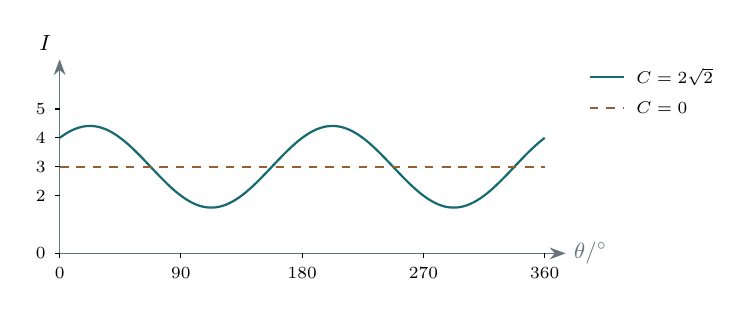
\begin{tikzpicture}[scale=.88,transform shape]
\draw[axis] (0,0.0)--(7.3,0.0) node[right] {$\theta/^\circ$};
\draw[axis] (0,0)--(0,2.8);
\node[above left] at (0,2.8) {$I$};
\draw[thin] (0.000000,0.0)--(0.000000,-0.06);\node[below,font=\scriptsize] at (0.000000,-0.08) {$ 0 $};
\draw[thin] (1.750000,0.0)--(1.750000,-0.06);\node[below,font=\scriptsize] at (1.750000,-0.08) {$ 90 $};
\draw[thin] (3.500000,0.0)--(3.500000,-0.06);\node[below,font=\scriptsize] at (3.500000,-0.08) {$ 180 $};
\draw[thin] (5.250000,0.0)--(5.250000,-0.06);\node[below,font=\scriptsize] at (5.250000,-0.08) {$ 270 $};
\draw[thin] (7.000000,0.0)--(7.000000,-0.06);\node[below,font=\scriptsize] at (7.000000,-0.08) {$ 360 $};
\draw[thin] (0,0.000000)--(-.06,0.000000);\node[left,font=\scriptsize] at (-.08,0.000000) {$ 0 $};
\draw[thin] (0,0.833333)--(-.06,0.833333);\node[left,font=\scriptsize] at (-.08,0.833333) {$ 2 $};
\draw[thin] (0,1.250000)--(-.06,1.250000);\node[left,font=\scriptsize] at (-.08,1.250000) {$ 3 $};
\draw[thin] (0,1.666667)--(-.06,1.666667);\node[left,font=\scriptsize] at (-.08,1.666667) {$ 4 $};
\draw[thin] (0,2.083333)--(-.06,2.083333);\node[left,font=\scriptsize] at (-.08,2.083333) {$ 5 $};
\draw[thick,color=accent] plot coordinates {(0.0000000,1.6666667) (0.0291667,1.6879023) (0.0583333,1.7079376) (0.0875000,1.7267178) (0.1166667,1.7441914) (0.1458333,1.7603104) (0.1750000,1.7750306) (0.2041667,1.7883118) (0.2333333,1.8001175) (0.2625000,1.8104154) (0.2916667,1.8191773) (0.3208333,1.8263790) (0.3500000,1.8320009) (0.3791667,1.8360276) (0.4083333,1.8384481) (0.4375000,1.8392557) (0.4666667,1.8384481) (0.4958333,1.8360276) (0.5250000,1.8320009) (0.5541667,1.8263790) (0.5833333,1.8191773) (0.6125000,1.8104154) (0.6416667,1.8001175) (0.6708333,1.7883118) (0.7000000,1.7750306) (0.7291667,1.7603104) (0.7583333,1.7441914) (0.7875000,1.7267178) (0.8166667,1.7079376) (0.8458333,1.6879023) (0.8750000,1.6666667) (0.9041667,1.6442890) (0.9333333,1.6208306) (0.9625000,1.5963558) (0.9916667,1.5709316) (1.0208333,1.5446278) (1.0500000,1.5175165) (1.0791667,1.4896719) (1.1083333,1.4611703) (1.1375000,1.4320900) (1.1666667,1.4025106) (1.1958333,1.3725131) (1.2250000,1.3421799) (1.2541667,1.3115940) (1.2833333,1.2808393) (1.3125000,1.2500000) (1.3416667,1.2191607) (1.3708333,1.1884060) (1.4000000,1.1578201) (1.4291667,1.1274869) (1.4583333,1.0974894) (1.4875000,1.0679100) (1.5166667,1.0388297) (1.5458333,1.0103281) (1.5750000,0.9824835) (1.6041667,0.9553722) (1.6333333,0.9290684) (1.6625000,0.9036442) (1.6916667,0.8791694) (1.7208333,0.8557110) (1.7500000,0.8333333) (1.7791667,0.8120977) (1.8083333,0.7920624) (1.8375000,0.7732822) (1.8666667,0.7558086) (1.8958333,0.7396896) (1.9250000,0.7249694) (1.9541667,0.7116882) (1.9833333,0.6998825) (2.0125000,0.6895846) (2.0416667,0.6808227) (2.0708333,0.6736210) (2.1000000,0.6679991) (2.1291667,0.6639724) (2.1583333,0.6615519) (2.1875000,0.6607443) (2.2166667,0.6615519) (2.2458333,0.6639724) (2.2750000,0.6679991) (2.3041667,0.6736210) (2.3333333,0.6808227) (2.3625000,0.6895846) (2.3916667,0.6998825) (2.4208333,0.7116882) (2.4500000,0.7249694) (2.4791667,0.7396896) (2.5083333,0.7558086) (2.5375000,0.7732822) (2.5666667,0.7920624) (2.5958333,0.8120977) (2.6250000,0.8333333) (2.6541667,0.8557110) (2.6833333,0.8791694) (2.7125000,0.9036442) (2.7416667,0.9290684) (2.7708333,0.9553722) (2.8000000,0.9824835) (2.8291667,1.0103281) (2.8583333,1.0388297) (2.8875000,1.0679100) (2.9166667,1.0974894) (2.9458333,1.1274869) (2.9750000,1.1578201) (3.0041667,1.1884060) (3.0333333,1.2191607) (3.0625000,1.2500000) (3.0916667,1.2808393) (3.1208333,1.3115940) (3.1500000,1.3421799) (3.1791667,1.3725131) (3.2083333,1.4025106) (3.2375000,1.4320900) (3.2666667,1.4611703) (3.2958333,1.4896719) (3.3250000,1.5175165) (3.3541667,1.5446278) (3.3833333,1.5709316) (3.4125000,1.5963558) (3.4416667,1.6208306) (3.4708333,1.6442890) (3.5000000,1.6666667) (3.5291667,1.6879023) (3.5583333,1.7079376) (3.5875000,1.7267178) (3.6166667,1.7441914) (3.6458333,1.7603104) (3.6750000,1.7750306) (3.7041667,1.7883118) (3.7333333,1.8001175) (3.7625000,1.8104154) (3.7916667,1.8191773) (3.8208333,1.8263790) (3.8500000,1.8320009) (3.8791667,1.8360276) (3.9083333,1.8384481) (3.9375000,1.8392557) (3.9666667,1.8384481) (3.9958333,1.8360276) (4.0250000,1.8320009) (4.0541667,1.8263790) (4.0833333,1.8191773) (4.1125000,1.8104154) (4.1416667,1.8001175) (4.1708333,1.7883118) (4.2000000,1.7750306) (4.2291667,1.7603104) (4.2583333,1.7441914) (4.2875000,1.7267178) (4.3166667,1.7079376) (4.3458333,1.6879023) (4.3750000,1.6666667) (4.4041667,1.6442890) (4.4333333,1.6208306) (4.4625000,1.5963558) (4.4916667,1.5709316) (4.5208333,1.5446278) (4.5500000,1.5175165) (4.5791667,1.4896719) (4.6083333,1.4611703) (4.6375000,1.4320900) (4.6666667,1.4025106) (4.6958333,1.3725131) (4.7250000,1.3421799) (4.7541667,1.3115940) (4.7833333,1.2808393) (4.8125000,1.2500000) (4.8416667,1.2191607) (4.8708333,1.1884060) (4.9000000,1.1578201) (4.9291667,1.1274869) (4.9583333,1.0974894) (4.9875000,1.0679100) (5.0166667,1.0388297) (5.0458333,1.0103281) (5.0750000,0.9824835) (5.1041667,0.9553722) (5.1333333,0.9290684) (5.1625000,0.9036442) (5.1916667,0.8791694) (5.2208333,0.8557110) (5.2500000,0.8333333) (5.2791667,0.8120977) (5.3083333,0.7920624) (5.3375000,0.7732822) (5.3666667,0.7558086) (5.3958333,0.7396896) (5.4250000,0.7249694) (5.4541667,0.7116882) (5.4833333,0.6998825) (5.5125000,0.6895846) (5.5416667,0.6808227) (5.5708333,0.6736210) (5.6000000,0.6679991) (5.6291667,0.6639724) (5.6583333,0.6615519) (5.6875000,0.6607443) (5.7166667,0.6615519) (5.7458333,0.6639724) (5.7750000,0.6679991) (5.8041667,0.6736210) (5.8333333,0.6808227) (5.8625000,0.6895846) (5.8916667,0.6998825) (5.9208333,0.7116882) (5.9500000,0.7249694) (5.9791667,0.7396896) (6.0083333,0.7558086) (6.0375000,0.7732822) (6.0666667,0.7920624) (6.0958333,0.8120977) (6.1250000,0.8333333) (6.1541667,0.8557110) (6.1833333,0.8791694) (6.2125000,0.9036442) (6.2416667,0.9290684) (6.2708333,0.9553722) (6.3000000,0.9824835) (6.3291667,1.0103281) (6.3583333,1.0388297) (6.3875000,1.0679100) (6.4166667,1.0974894) (6.4458333,1.1274869) (6.4750000,1.1578201) (6.5041667,1.1884060) (6.5333333,1.2191607) (6.5625000,1.2500000) (6.5916667,1.2808393) (6.6208333,1.3115940) (6.6500000,1.3421799) (6.6791667,1.3725131) (6.7083333,1.4025106) (6.7375000,1.4320900) (6.7666667,1.4611703) (6.7958333,1.4896719) (6.8250000,1.5175165) (6.8541667,1.5446278) (6.8833333,1.5709316) (6.9125000,1.5963558) (6.9416667,1.6208306) (6.9708333,1.6442890) (7.0000000,1.6666667)};
\draw[thick,color=accent] (7.65,2.55)--(8.15,2.55);\node[right,font=\scriptsize] at (8.2,2.55) {$C=2\sqrt2$};
\draw[thick,dashed,color=warm] plot coordinates {(0.0000000,1.2500000) (0.0291667,1.2500000) (0.0583333,1.2500000) (0.0875000,1.2500000) (0.1166667,1.2500000) (0.1458333,1.2500000) (0.1750000,1.2500000) (0.2041667,1.2500000) (0.2333333,1.2500000) (0.2625000,1.2500000) (0.2916667,1.2500000) (0.3208333,1.2500000) (0.3500000,1.2500000) (0.3791667,1.2500000) (0.4083333,1.2500000) (0.4375000,1.2500000) (0.4666667,1.2500000) (0.4958333,1.2500000) (0.5250000,1.2500000) (0.5541667,1.2500000) (0.5833333,1.2500000) (0.6125000,1.2500000) (0.6416667,1.2500000) (0.6708333,1.2500000) (0.7000000,1.2500000) (0.7291667,1.2500000) (0.7583333,1.2500000) (0.7875000,1.2500000) (0.8166667,1.2500000) (0.8458333,1.2500000) (0.8750000,1.2500000) (0.9041667,1.2500000) (0.9333333,1.2500000) (0.9625000,1.2500000) (0.9916667,1.2500000) (1.0208333,1.2500000) (1.0500000,1.2500000) (1.0791667,1.2500000) (1.1083333,1.2500000) (1.1375000,1.2500000) (1.1666667,1.2500000) (1.1958333,1.2500000) (1.2250000,1.2500000) (1.2541667,1.2500000) (1.2833333,1.2500000) (1.3125000,1.2500000) (1.3416667,1.2500000) (1.3708333,1.2500000) (1.4000000,1.2500000) (1.4291667,1.2500000) (1.4583333,1.2500000) (1.4875000,1.2500000) (1.5166667,1.2500000) (1.5458333,1.2500000) (1.5750000,1.2500000) (1.6041667,1.2500000) (1.6333333,1.2500000) (1.6625000,1.2500000) (1.6916667,1.2500000) (1.7208333,1.2500000) (1.7500000,1.2500000) (1.7791667,1.2500000) (1.8083333,1.2500000) (1.8375000,1.2500000) (1.8666667,1.2500000) (1.8958333,1.2500000) (1.9250000,1.2500000) (1.9541667,1.2500000) (1.9833333,1.2500000) (2.0125000,1.2500000) (2.0416667,1.2500000) (2.0708333,1.2500000) (2.1000000,1.2500000) (2.1291667,1.2500000) (2.1583333,1.2500000) (2.1875000,1.2500000) (2.2166667,1.2500000) (2.2458333,1.2500000) (2.2750000,1.2500000) (2.3041667,1.2500000) (2.3333333,1.2500000) (2.3625000,1.2500000) (2.3916667,1.2500000) (2.4208333,1.2500000) (2.4500000,1.2500000) (2.4791667,1.2500000) (2.5083333,1.2500000) (2.5375000,1.2500000) (2.5666667,1.2500000) (2.5958333,1.2500000) (2.6250000,1.2500000) (2.6541667,1.2500000) (2.6833333,1.2500000) (2.7125000,1.2500000) (2.7416667,1.2500000) (2.7708333,1.2500000) (2.8000000,1.2500000) (2.8291667,1.2500000) (2.8583333,1.2500000) (2.8875000,1.2500000) (2.9166667,1.2500000) (2.9458333,1.2500000) (2.9750000,1.2500000) (3.0041667,1.2500000) (3.0333333,1.2500000) (3.0625000,1.2500000) (3.0916667,1.2500000) (3.1208333,1.2500000) (3.1500000,1.2500000) (3.1791667,1.2500000) (3.2083333,1.2500000) (3.2375000,1.2500000) (3.2666667,1.2500000) (3.2958333,1.2500000) (3.3250000,1.2500000) (3.3541667,1.2500000) (3.3833333,1.2500000) (3.4125000,1.2500000) (3.4416667,1.2500000) (3.4708333,1.2500000) (3.5000000,1.2500000) (3.5291667,1.2500000) (3.5583333,1.2500000) (3.5875000,1.2500000) (3.6166667,1.2500000) (3.6458333,1.2500000) (3.6750000,1.2500000) (3.7041667,1.2500000) (3.7333333,1.2500000) (3.7625000,1.2500000) (3.7916667,1.2500000) (3.8208333,1.2500000) (3.8500000,1.2500000) (3.8791667,1.2500000) (3.9083333,1.2500000) (3.9375000,1.2500000) (3.9666667,1.2500000) (3.9958333,1.2500000) (4.0250000,1.2500000) (4.0541667,1.2500000) (4.0833333,1.2500000) (4.1125000,1.2500000) (4.1416667,1.2500000) (4.1708333,1.2500000) (4.2000000,1.2500000) (4.2291667,1.2500000) (4.2583333,1.2500000) (4.2875000,1.2500000) (4.3166667,1.2500000) (4.3458333,1.2500000) (4.3750000,1.2500000) (4.4041667,1.2500000) (4.4333333,1.2500000) (4.4625000,1.2500000) (4.4916667,1.2500000) (4.5208333,1.2500000) (4.5500000,1.2500000) (4.5791667,1.2500000) (4.6083333,1.2500000) (4.6375000,1.2500000) (4.6666667,1.2500000) (4.6958333,1.2500000) (4.7250000,1.2500000) (4.7541667,1.2500000) (4.7833333,1.2500000) (4.8125000,1.2500000) (4.8416667,1.2500000) (4.8708333,1.2500000) (4.9000000,1.2500000) (4.9291667,1.2500000) (4.9583333,1.2500000) (4.9875000,1.2500000) (5.0166667,1.2500000) (5.0458333,1.2500000) (5.0750000,1.2500000) (5.1041667,1.2500000) (5.1333333,1.2500000) (5.1625000,1.2500000) (5.1916667,1.2500000) (5.2208333,1.2500000) (5.2500000,1.2500000) (5.2791667,1.2500000) (5.3083333,1.2500000) (5.3375000,1.2500000) (5.3666667,1.2500000) (5.3958333,1.2500000) (5.4250000,1.2500000) (5.4541667,1.2500000) (5.4833333,1.2500000) (5.5125000,1.2500000) (5.5416667,1.2500000) (5.5708333,1.2500000) (5.6000000,1.2500000) (5.6291667,1.2500000) (5.6583333,1.2500000) (5.6875000,1.2500000) (5.7166667,1.2500000) (5.7458333,1.2500000) (5.7750000,1.2500000) (5.8041667,1.2500000) (5.8333333,1.2500000) (5.8625000,1.2500000) (5.8916667,1.2500000) (5.9208333,1.2500000) (5.9500000,1.2500000) (5.9791667,1.2500000) (6.0083333,1.2500000) (6.0375000,1.2500000) (6.0666667,1.2500000) (6.0958333,1.2500000) (6.1250000,1.2500000) (6.1541667,1.2500000) (6.1833333,1.2500000) (6.2125000,1.2500000) (6.2416667,1.2500000) (6.2708333,1.2500000) (6.3000000,1.2500000) (6.3291667,1.2500000) (6.3583333,1.2500000) (6.3875000,1.2500000) (6.4166667,1.2500000) (6.4458333,1.2500000) (6.4750000,1.2500000) (6.5041667,1.2500000) (6.5333333,1.2500000) (6.5625000,1.2500000) (6.5916667,1.2500000) (6.6208333,1.2500000) (6.6500000,1.2500000) (6.6791667,1.2500000) (6.7083333,1.2500000) (6.7375000,1.2500000) (6.7666667,1.2500000) (6.7958333,1.2500000) (6.8250000,1.2500000) (6.8541667,1.2500000) (6.8833333,1.2500000) (6.9125000,1.2500000) (6.9416667,1.2500000) (6.9708333,1.2500000) (7.0000000,1.2500000)};
\draw[thick,dashed,color=warm] (7.65,2.0999999999999996)--(8.15,2.0999999999999996);\node[right,font=\scriptsize] at (8.2,2.0999999999999996) {$C=0$};
\end{tikzpicture}
\figcaption{解图光4.2B\quad 非零调制具有离散极值轴，恒强退化没有唯一轴}
\end{minipage}\end{center}

\textbf{检偏等效不等于完整状态相同。}线检偏结果只含$S_0,S_1,S_2$，所以所有具有这三个量而$S_3$不同的状态都给同一条曲线。构造的自然光强$S_0-C$与线偏光强$C$之和仍为$S_0$，方向为$\theta_0$；它对任何理想线轴的投影都正确。若入射本身有$S_3\ne0$，这一构造没有保留圆偏相关，不能在任意后续光学装置前继续等同。

例如Jones矢量$(2,i)$的相干矩阵有$(S_0,S_1,S_2,S_3)=(5,3,0,4)$，完全偏振度为1；强度2的自然光与强度3、沿$x$的线偏振光混合则有$(5,3,0,0)$，总偏振度为$3/5$。两者在线检偏时都给$I=1+3\cos^2\theta$。加入场矩阵$\mathsf Q=\operatorname{diag}(1,-i)$的四分之一波片后，新的$S_2$等于原$S_3$，故两条曲线分别变成$[5+3\cos2\theta+4\sin2\theta]/2$与$[5+3\cos2\theta]/2$。图C比较同一线检偏曲线所对应的不同完整偏振态。

\begin{center}\begin{minipage}{.98\linewidth}\centering
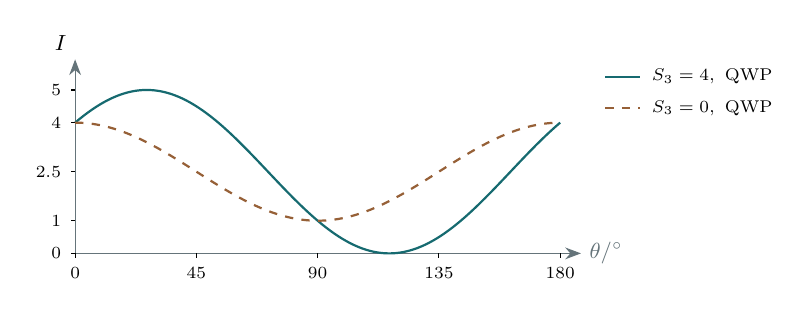
\begin{tikzpicture}[scale=.88,transform shape]
\draw[axis] (0,0.0)--(7.3,0.0) node[right] {$\theta/^\circ$};
\draw[axis] (0,0)--(0,2.8);
\node[above left] at (0,2.8) {$I$};
\draw[thin] (0.000000,0.0)--(0.000000,-0.06);\node[below,font=\scriptsize] at (0.000000,-0.08) {$ 0 $};
\draw[thin] (1.750000,0.0)--(1.750000,-0.06);\node[below,font=\scriptsize] at (1.750000,-0.08) {$ 45 $};
\draw[thin] (3.500000,0.0)--(3.500000,-0.06);\node[below,font=\scriptsize] at (3.500000,-0.08) {$ 90 $};
\draw[thin] (5.250000,0.0)--(5.250000,-0.06);\node[below,font=\scriptsize] at (5.250000,-0.08) {$ 135 $};
\draw[thin] (7.000000,0.0)--(7.000000,-0.06);\node[below,font=\scriptsize] at (7.000000,-0.08) {$ 180 $};
\draw[thin] (0,0.000000)--(-.06,0.000000);\node[left,font=\scriptsize] at (-.08,0.000000) {$ 0 $};
\draw[thin] (0,0.471698)--(-.06,0.471698);\node[left,font=\scriptsize] at (-.08,0.471698) {$ 1 $};
\draw[thin] (0,1.179245)--(-.06,1.179245);\node[left,font=\scriptsize] at (-.08,1.179245) {$ 2.5 $};
\draw[thin] (0,1.886792)--(-.06,1.886792);\node[left,font=\scriptsize] at (-.08,1.886792) {$ 4 $};
\draw[thin] (0,2.358491)--(-.06,2.358491);\node[left,font=\scriptsize] at (-.08,2.358491) {$ 5 $};
\draw[thick,color=accent] plot coordinates {(0.0000000,1.8867925) (0.0291667,1.9112452) (0.0583333,1.9351963) (0.0875000,1.9586293) (0.1166667,1.9815282) (0.1458333,2.0038772) (0.1750000,2.0256611) (0.2041667,2.0468648) (0.2333333,2.0674740) (0.2625000,2.0874743) (0.2916667,2.1068523) (0.3208333,2.1255945) (0.3500000,2.1436881) (0.3791667,2.1611207) (0.4083333,2.1778804) (0.4375000,2.1939557) (0.4666667,2.2093356) (0.4958333,2.2240095) (0.5250000,2.2379674) (0.5541667,2.2511996) (0.5833333,2.2636972) (0.6125000,2.2754516) (0.6416667,2.2864547) (0.6708333,2.2966989) (0.7000000,2.3061774) (0.7291667,2.3148834) (0.7583333,2.3228112) (0.7875000,2.3299552) (0.8166667,2.3363106) (0.8458333,2.3418730) (0.8750000,2.3466386) (0.9041667,2.3506041) (0.9333333,2.3537668) (0.9625000,2.3561245) (0.9916667,2.3576757) (1.0208333,2.3584193) (1.0500000,2.3583547) (1.0791667,2.3574819) (1.1083333,2.3558017) (1.1375000,2.3533152) (1.1666667,2.3500240) (1.1958333,2.3459304) (1.2250000,2.3410372) (1.2541667,2.3353477) (1.2833333,2.3288660) (1.3125000,2.3215963) (1.3416667,2.3135438) (1.3708333,2.3047138) (1.4000000,2.2951125) (1.4291667,2.2847465) (1.4583333,2.2736227) (1.4875000,2.2617490) (1.5166667,2.2491334) (1.5458333,2.2357845) (1.5750000,2.2217115) (1.6041667,2.2069241) (1.6333333,2.1914323) (1.6625000,2.1752468) (1.6916667,2.1583788) (1.7208333,2.1408397) (1.7500000,2.1226415) (1.7791667,2.1037968) (1.8083333,2.0843185) (1.8375000,2.0642198) (1.8666667,2.0435147) (1.8958333,2.0222172) (1.9250000,2.0003420) (1.9541667,1.9779040) (1.9833333,1.9549187) (2.0125000,1.9314018) (2.0416667,1.9073694) (2.0708333,1.8828379) (2.1000000,1.8578243) (2.1291667,1.8323456) (2.1583333,1.8064193) (2.1875000,1.7800632) (2.2166667,1.7532953) (2.2458333,1.7261339) (2.2750000,1.6985978) (2.3041667,1.6707057) (2.3333333,1.6424768) (2.3625000,1.6139304) (2.3916667,1.5850861) (2.4208333,1.5559637) (2.4500000,1.5265831) (2.4791667,1.4969644) (2.5083333,1.4671280) (2.5375000,1.4370943) (2.5666667,1.4068838) (2.5958333,1.3765174) (2.6250000,1.3460158) (2.6541667,1.3153998) (2.6833333,1.2846906) (2.7125000,1.2539090) (2.7416667,1.2230763) (2.7708333,1.1922136) (2.8000000,1.1613420) (2.8291667,1.1304826) (2.8583333,1.0996567) (2.8875000,1.0688853) (2.9166667,1.0381896) (2.9458333,1.0075905) (2.9750000,0.9771091) (3.0041667,0.9467662) (3.0333333,0.9165826) (3.0625000,0.8865790) (3.0916667,0.8567761) (3.1208333,0.8271941) (3.1500000,0.7978534) (3.1791667,0.7687741) (3.2083333,0.7399761) (3.2375000,0.7114792) (3.2666667,0.6833028) (3.2958333,0.6554664) (3.3250000,0.6279889) (3.3541667,0.6008892) (3.3833333,0.5741859) (3.4125000,0.5478973) (3.4416667,0.5220413) (3.4708333,0.4966358) (3.5000000,0.4716981) (3.5291667,0.4472453) (3.5583333,0.4232942) (3.5875000,0.3998612) (3.6166667,0.3769624) (3.6458333,0.3546134) (3.6750000,0.3328295) (3.7041667,0.3116257) (3.7333333,0.2910166) (3.7625000,0.2710162) (3.7916667,0.2516383) (3.8208333,0.2328961) (3.8500000,0.2148025) (3.8791667,0.1973698) (3.9083333,0.1806101) (3.9375000,0.1645348) (3.9666667,0.1491550) (3.9958333,0.1344811) (4.0250000,0.1205232) (4.0541667,0.1072909) (4.0833333,0.0947933) (4.1125000,0.0830390) (4.1416667,0.0720359) (4.1708333,0.0617916) (4.2000000,0.0523132) (4.2291667,0.0436071) (4.2583333,0.0356794) (4.2875000,0.0285354) (4.3166667,0.0221800) (4.3458333,0.0166176) (4.3750000,0.0118520) (4.4041667,0.0078865) (4.4333333,0.0047238) (4.4625000,0.0023660) (4.4916667,0.0008149) (4.5208333,0.0000713) (4.5500000,0.0001359) (4.5791667,0.0010086) (4.6083333,0.0026888) (4.6375000,0.0051754) (4.6666667,0.0084666) (4.6958333,0.0125602) (4.7250000,0.0174534) (4.7541667,0.0231428) (4.7833333,0.0296246) (4.8125000,0.0368942) (4.8416667,0.0449468) (4.8708333,0.0537768) (4.9000000,0.0633781) (4.9291667,0.0737441) (4.9583333,0.0848678) (4.9875000,0.0967416) (5.0166667,0.1093572) (5.0458333,0.1227061) (5.0750000,0.1367791) (5.1041667,0.1515665) (5.1333333,0.1670583) (5.1625000,0.1832437) (5.1916667,0.2001118) (5.2208333,0.2176509) (5.2500000,0.2358491) (5.2791667,0.2546938) (5.3083333,0.2741721) (5.3375000,0.2942707) (5.3666667,0.3149759) (5.3958333,0.3362734) (5.4250000,0.3581486) (5.4541667,0.3805865) (5.4833333,0.4035719) (5.5125000,0.4270888) (5.5416667,0.4511212) (5.5708333,0.4756526) (5.6000000,0.5006663) (5.6291667,0.5261450) (5.6583333,0.5520713) (5.6875000,0.5784274) (5.7166667,0.6051953) (5.7458333,0.6323566) (5.7750000,0.6598928) (5.8041667,0.6877849) (5.8333333,0.7160138) (5.8625000,0.7445602) (5.8916667,0.7734044) (5.9208333,0.8025269) (5.9500000,0.8319075) (5.9791667,0.8615262) (6.0083333,0.8913626) (6.0375000,0.9213963) (6.0666667,0.9516067) (6.0958333,0.9819732) (6.1250000,1.0124748) (6.1541667,1.0430908) (6.1833333,1.0738000) (6.2125000,1.1045815) (6.2416667,1.1354142) (6.2708333,1.1662770) (6.3000000,1.1971486) (6.3291667,1.2280079) (6.3583333,1.2588339) (6.3875000,1.2896052) (6.4166667,1.3203010) (6.4458333,1.3509001) (6.4750000,1.3813815) (6.5041667,1.4117244) (6.5333333,1.4419080) (6.5625000,1.4719115) (6.5916667,1.5017145) (6.6208333,1.5312965) (6.6500000,1.5606372) (6.6791667,1.5897165) (6.7083333,1.6185145) (6.7375000,1.6470114) (6.7666667,1.6751877) (6.7958333,1.7030242) (6.8250000,1.7305017) (6.8541667,1.7576014) (6.8833333,1.7843047) (6.9125000,1.8105933) (6.9416667,1.8364492) (6.9708333,1.8618548) (7.0000000,1.8867925)};
\draw[thick,color=accent] (7.65,2.55)--(8.15,2.55);\node[right,font=\scriptsize] at (8.2,2.55) {$S_3=4,\ \mathrm{QWP}$};
\draw[thick,dashed,color=warm] plot coordinates {(0.0000000,1.8867925) (0.0291667,1.8865500) (0.0583333,1.8858228) (0.0875000,1.8846113) (0.1166667,1.8829164) (0.1458333,1.8807393) (0.1750000,1.8780814) (0.2041667,1.8749445) (0.2333333,1.8713308) (0.2625000,1.8672429) (0.2916667,1.8626834) (0.3208333,1.8576555) (0.3500000,1.8521626) (0.3791667,1.8462086) (0.4083333,1.8397975) (0.4375000,1.8329336) (0.4666667,1.8256218) (0.4958333,1.8178669) (0.5250000,1.8096744) (0.5541667,1.8010498) (0.5833333,1.7919991) (0.6125000,1.7825284) (0.6416667,1.7726443) (0.6708333,1.7623534) (0.7000000,1.7516630) (0.7291667,1.7405802) (0.7583333,1.7291127) (0.7875000,1.7172684) (0.8166667,1.7050553) (0.8458333,1.6924819) (0.8750000,1.6795567) (0.9041667,1.6662886) (0.9333333,1.6526867) (0.9625000,1.6387604) (0.9916667,1.6245191) (1.0208333,1.6099727) (1.0500000,1.5951311) (1.0791667,1.5800044) (1.1083333,1.5646031) (1.1375000,1.5489377) (1.1666667,1.5330189) (1.1958333,1.5168576) (1.2250000,1.5004650) (1.2541667,1.4838522) (1.2833333,1.4670306) (1.3125000,1.4500119) (1.3416667,1.4328075) (1.3708333,1.4154294) (1.4000000,1.3978894) (1.4291667,1.3801995) (1.4583333,1.3623720) (1.4875000,1.3444189) (1.5166667,1.3263526) (1.5458333,1.3081855) (1.5750000,1.2899300) (1.6041667,1.2715987) (1.6333333,1.2532041) (1.6625000,1.2347588) (1.6916667,1.2162754) (1.7208333,1.1977667) (1.7500000,1.1792453) (1.7791667,1.1607239) (1.8083333,1.1422151) (1.8375000,1.1237318) (1.8666667,1.1052865) (1.8958333,1.0868918) (1.9250000,1.0685605) (1.9541667,1.0503051) (1.9833333,1.0321380) (2.0125000,1.0140717) (2.0416667,0.9961186) (2.0708333,0.9782910) (2.1000000,0.9606012) (2.1291667,0.9430612) (2.1583333,0.9256831) (2.1875000,0.9084787) (2.2166667,0.8914599) (2.2458333,0.8746384) (2.2750000,0.8580256) (2.3041667,0.8416330) (2.3333333,0.8254717) (2.3625000,0.8095529) (2.3916667,0.7938875) (2.4208333,0.7784862) (2.4500000,0.7633595) (2.4791667,0.7485179) (2.5083333,0.7339714) (2.5375000,0.7197302) (2.5666667,0.7058038) (2.5958333,0.6922020) (2.6250000,0.6789339) (2.6541667,0.6660087) (2.6833333,0.6534353) (2.7125000,0.6412222) (2.7416667,0.6293779) (2.7708333,0.6179104) (2.8000000,0.6068276) (2.8291667,0.5961371) (2.8583333,0.5858463) (2.8875000,0.5759621) (2.9166667,0.5664915) (2.9458333,0.5574407) (2.9750000,0.5488161) (3.0041667,0.5406236) (3.0333333,0.5328688) (3.0625000,0.5255569) (3.0916667,0.5186931) (3.1208333,0.5122820) (3.1500000,0.5063279) (3.1791667,0.5008351) (3.2083333,0.4958072) (3.2375000,0.4912477) (3.2666667,0.4871597) (3.2958333,0.4835461) (3.3250000,0.4804092) (3.3541667,0.4777513) (3.3833333,0.4755741) (3.4125000,0.4738792) (3.4416667,0.4726678) (3.4708333,0.4719406) (3.5000000,0.4716981) (3.5291667,0.4719406) (3.5583333,0.4726678) (3.5875000,0.4738792) (3.6166667,0.4755741) (3.6458333,0.4777513) (3.6750000,0.4804092) (3.7041667,0.4835461) (3.7333333,0.4871597) (3.7625000,0.4912477) (3.7916667,0.4958072) (3.8208333,0.5008351) (3.8500000,0.5063279) (3.8791667,0.5122820) (3.9083333,0.5186931) (3.9375000,0.5255569) (3.9666667,0.5328688) (3.9958333,0.5406236) (4.0250000,0.5488161) (4.0541667,0.5574407) (4.0833333,0.5664915) (4.1125000,0.5759621) (4.1416667,0.5858463) (4.1708333,0.5961371) (4.2000000,0.6068276) (4.2291667,0.6179104) (4.2583333,0.6293779) (4.2875000,0.6412222) (4.3166667,0.6534353) (4.3458333,0.6660087) (4.3750000,0.6789339) (4.4041667,0.6922020) (4.4333333,0.7058038) (4.4625000,0.7197302) (4.4916667,0.7339714) (4.5208333,0.7485179) (4.5500000,0.7633595) (4.5791667,0.7784862) (4.6083333,0.7938875) (4.6375000,0.8095529) (4.6666667,0.8254717) (4.6958333,0.8416330) (4.7250000,0.8580256) (4.7541667,0.8746384) (4.7833333,0.8914599) (4.8125000,0.9084787) (4.8416667,0.9256831) (4.8708333,0.9430612) (4.9000000,0.9606012) (4.9291667,0.9782910) (4.9583333,0.9961186) (4.9875000,1.0140717) (5.0166667,1.0321380) (5.0458333,1.0503051) (5.0750000,1.0685605) (5.1041667,1.0868918) (5.1333333,1.1052865) (5.1625000,1.1237318) (5.1916667,1.1422151) (5.2208333,1.1607239) (5.2500000,1.1792453) (5.2791667,1.1977667) (5.3083333,1.2162754) (5.3375000,1.2347588) (5.3666667,1.2532041) (5.3958333,1.2715987) (5.4250000,1.2899300) (5.4541667,1.3081855) (5.4833333,1.3263526) (5.5125000,1.3444189) (5.5416667,1.3623720) (5.5708333,1.3801995) (5.6000000,1.3978894) (5.6291667,1.4154294) (5.6583333,1.4328075) (5.6875000,1.4500119) (5.7166667,1.4670306) (5.7458333,1.4838522) (5.7750000,1.5004650) (5.8041667,1.5168576) (5.8333333,1.5330189) (5.8625000,1.5489377) (5.8916667,1.5646031) (5.9208333,1.5800044) (5.9500000,1.5951311) (5.9791667,1.6099727) (6.0083333,1.6245191) (6.0375000,1.6387604) (6.0666667,1.6526867) (6.0958333,1.6662886) (6.1250000,1.6795567) (6.1541667,1.6924819) (6.1833333,1.7050553) (6.2125000,1.7172684) (6.2416667,1.7291127) (6.2708333,1.7405802) (6.3000000,1.7516630) (6.3291667,1.7623534) (6.3583333,1.7726443) (6.3875000,1.7825284) (6.4166667,1.7919991) (6.4458333,1.8010498) (6.4750000,1.8096744) (6.5041667,1.8178669) (6.5333333,1.8256218) (6.5625000,1.8329336) (6.5916667,1.8397975) (6.6208333,1.8462086) (6.6500000,1.8521626) (6.6791667,1.8576555) (6.7083333,1.8626834) (6.7375000,1.8672429) (6.7666667,1.8713308) (6.7958333,1.8749445) (6.8250000,1.8780814) (6.8541667,1.8807393) (6.8833333,1.8829164) (6.9125000,1.8846113) (6.9416667,1.8858228) (6.9708333,1.8865500) (7.0000000,1.8867925)};
\draw[thick,dashed,color=warm] (7.65,2.0999999999999996)--(8.15,2.0999999999999996);\node[right,font=\scriptsize] at (8.2,2.0999999999999996) {$S_3=0,\ \mathrm{QWP}$};
\end{tikzpicture}
\figcaption{解图光4.2C\quad 相同线检偏结果在插入相同相位片后分开}
\end{minipage}\end{center}

如果要分解完整相干矩阵，应按其两个本征值$(S_0\pm\sqrt{S_1^2+S_2^2+S_3^2})/2$处理：一般得到自然光与完全椭圆偏振光的叠加，而不一定是自然光与线偏振光。只测线检偏时，可能的总偏振度范围为$P_L\le P\le1$，需额外相位片测量才可缩小这个范围。

\textbf{用有限读数还原旋转曲线。}三个方向即可给出
\[
S_0=I(0)+I(\pi/2),\quad S_1=I(0)-I(\pi/2),\quad
S_2=2I(\pi/4)-S_0.
\]
再测$3\pi/4$作一致性检查，要求$I(\pi/4)+I(3\pi/4)=S_0$。图D用$4,4,2$三个读数还原$S_0=6,S_1=S_2=2$；主轴是$\tfrac12\operatorname{atan2}(2,2)=22.5^\circ$，不是向量本身的$45^\circ$。由$C=2\sqrt2$得极值$3\pm\sqrt2$，不能只取这三个采样点中最大的读数当成真正最大值。

\begin{center}\begin{minipage}{.98\linewidth}\centering
\begin{tikzpicture}[scale=.88,transform shape]
\draw[axis] (0,0.0)--(7.3,0.0) node[right] {$\theta/^\circ$};
\draw[axis] (0,0)--(0,2.8);
\node[above left] at (0,2.8) {$I$};
\draw[thin] (0.000000,0.0)--(0.000000,-0.06);\node[below,font=\scriptsize] at (0.000000,-0.08) {$ 0 $};
\draw[thin] (0.875000,0.0)--(0.875000,-0.06);\node[below,font=\scriptsize] at (0.875000,-0.08) {$ 22.5 $};
\draw[thin] (1.750000,0.0)--(1.750000,-0.06);\node[below,font=\scriptsize] at (1.750000,-0.08) {$ 45 $};
\draw[thin] (3.500000,0.0)--(3.500000,-0.06);\node[below,font=\scriptsize] at (3.500000,-0.08) {$ 90 $};
\draw[thin] (5.250000,0.0)--(5.250000,-0.06);\node[below,font=\scriptsize] at (5.250000,-0.08) {$ 135 $};
\draw[thin] (7.000000,0.0)--(7.000000,-0.06);\node[below,font=\scriptsize] at (7.000000,-0.08) {$ 180 $};
\draw[thin] (0,0.000000)--(-.06,0.000000);\node[left,font=\scriptsize] at (-.08,0.000000) {$ 0 $};
\draw[thin] (0,1.000000)--(-.06,1.000000);\node[left,font=\scriptsize] at (-.08,1.000000) {$ 2 $};
\draw[thin] (0,1.500000)--(-.06,1.500000);\node[left,font=\scriptsize] at (-.08,1.500000) {$ 3 $};
\draw[thin] (0,2.000000)--(-.06,2.000000);\node[left,font=\scriptsize] at (-.08,2.000000) {$ 4 $};
\draw[thick,color=accent] plot coordinates {(0.0000000,2.0000000) (0.0291667,2.0129171) (0.0583333,2.0254827) (0.0875000,2.0376882) (0.1166667,2.0495252) (0.1458333,2.0609855) (0.1750000,2.0720614) (0.2041667,2.0827452) (0.2333333,2.0930296) (0.2625000,2.1029076) (0.2916667,2.1123724) (0.3208333,2.1214175) (0.3500000,2.1300368) (0.3791667,2.1382242) (0.4083333,2.1459742) (0.4375000,2.1532815) (0.4666667,2.1601411) (0.4958333,2.1665482) (0.5250000,2.1724985) (0.5541667,2.1779879) (0.5833333,2.1830127) (0.6125000,2.1875694) (0.6416667,2.1916548) (0.6708333,2.1952662) (0.7000000,2.1984011) (0.7291667,2.2010574) (0.7583333,2.2032332) (0.7875000,2.2049270) (0.8166667,2.2061377) (0.8458333,2.2068645) (0.8750000,2.2071068) (0.9041667,2.2068645) (0.9333333,2.2061377) (0.9625000,2.2049270) (0.9916667,2.2032332) (1.0208333,2.2010574) (1.0500000,2.1984011) (1.0791667,2.1952662) (1.1083333,2.1916548) (1.1375000,2.1875694) (1.1666667,2.1830127) (1.1958333,2.1779879) (1.2250000,2.1724985) (1.2541667,2.1665482) (1.2833333,2.1601411) (1.3125000,2.1532815) (1.3416667,2.1459742) (1.3708333,2.1382242) (1.4000000,2.1300368) (1.4291667,2.1214175) (1.4583333,2.1123724) (1.4875000,2.1029076) (1.5166667,2.0930296) (1.5458333,2.0827452) (1.5750000,2.0720614) (1.6041667,2.0609855) (1.6333333,2.0495252) (1.6625000,2.0376882) (1.6916667,2.0254827) (1.7208333,2.0129171) (1.7500000,2.0000000) (1.7791667,1.9867402) (1.8083333,1.9731468) (1.8375000,1.9592291) (1.8666667,1.9449967) (1.8958333,1.9304593) (1.9250000,1.9156269) (1.9541667,1.9005097) (1.9833333,1.8851180) (2.0125000,1.8694623) (2.0416667,1.8535534) (2.0708333,1.8374022) (2.1000000,1.8210198) (2.1291667,1.8044173) (2.1583333,1.7876062) (2.1875000,1.7705981) (2.2166667,1.7534044) (2.2458333,1.7360371) (2.2750000,1.7185080) (2.3041667,1.7008292) (2.3333333,1.6830127) (2.3625000,1.6650708) (2.3916667,1.6470158) (2.4208333,1.6288600) (2.4500000,1.6106159) (2.4791667,1.5922960) (2.5083333,1.5739128) (2.5375000,1.5554790) (2.5666667,1.5370071) (2.5958333,1.5185099) (2.6250000,1.5000000) (2.6541667,1.4814901) (2.6833333,1.4629929) (2.7125000,1.4445210) (2.7416667,1.4260872) (2.7708333,1.4077040) (2.8000000,1.3893841) (2.8291667,1.3711400) (2.8583333,1.3529842) (2.8875000,1.3349292) (2.9166667,1.3169873) (2.9458333,1.2991708) (2.9750000,1.2814920) (3.0041667,1.2639629) (3.0333333,1.2465956) (3.0625000,1.2294019) (3.0916667,1.2123938) (3.1208333,1.1955827) (3.1500000,1.1789802) (3.1791667,1.1625978) (3.2083333,1.1464466) (3.2375000,1.1305377) (3.2666667,1.1148820) (3.2958333,1.0994903) (3.3250000,1.0843731) (3.3541667,1.0695407) (3.3833333,1.0550033) (3.4125000,1.0407709) (3.4416667,1.0268532) (3.4708333,1.0132598) (3.5000000,1.0000000) (3.5291667,0.9870829) (3.5583333,0.9745173) (3.5875000,0.9623118) (3.6166667,0.9504748) (3.6458333,0.9390145) (3.6750000,0.9279386) (3.7041667,0.9172548) (3.7333333,0.9069704) (3.7625000,0.8970924) (3.7916667,0.8876276) (3.8208333,0.8785825) (3.8500000,0.8699632) (3.8791667,0.8617758) (3.9083333,0.8540258) (3.9375000,0.8467185) (3.9666667,0.8398589) (3.9958333,0.8334518) (4.0250000,0.8275015) (4.0541667,0.8220121) (4.0833333,0.8169873) (4.1125000,0.8124306) (4.1416667,0.8083452) (4.1708333,0.8047338) (4.2000000,0.8015989) (4.2291667,0.7989426) (4.2583333,0.7967668) (4.2875000,0.7950730) (4.3166667,0.7938623) (4.3458333,0.7931355) (4.3750000,0.7928932) (4.4041667,0.7931355) (4.4333333,0.7938623) (4.4625000,0.7950730) (4.4916667,0.7967668) (4.5208333,0.7989426) (4.5500000,0.8015989) (4.5791667,0.8047338) (4.6083333,0.8083452) (4.6375000,0.8124306) (4.6666667,0.8169873) (4.6958333,0.8220121) (4.7250000,0.8275015) (4.7541667,0.8334518) (4.7833333,0.8398589) (4.8125000,0.8467185) (4.8416667,0.8540258) (4.8708333,0.8617758) (4.9000000,0.8699632) (4.9291667,0.8785825) (4.9583333,0.8876276) (4.9875000,0.8970924) (5.0166667,0.9069704) (5.0458333,0.9172548) (5.0750000,0.9279386) (5.1041667,0.9390145) (5.1333333,0.9504748) (5.1625000,0.9623118) (5.1916667,0.9745173) (5.2208333,0.9870829) (5.2500000,1.0000000) (5.2791667,1.0132598) (5.3083333,1.0268532) (5.3375000,1.0407709) (5.3666667,1.0550033) (5.3958333,1.0695407) (5.4250000,1.0843731) (5.4541667,1.0994903) (5.4833333,1.1148820) (5.5125000,1.1305377) (5.5416667,1.1464466) (5.5708333,1.1625978) (5.6000000,1.1789802) (5.6291667,1.1955827) (5.6583333,1.2123938) (5.6875000,1.2294019) (5.7166667,1.2465956) (5.7458333,1.2639629) (5.7750000,1.2814920) (5.8041667,1.2991708) (5.8333333,1.3169873) (5.8625000,1.3349292) (5.8916667,1.3529842) (5.9208333,1.3711400) (5.9500000,1.3893841) (5.9791667,1.4077040) (6.0083333,1.4260872) (6.0375000,1.4445210) (6.0666667,1.4629929) (6.0958333,1.4814901) (6.1250000,1.5000000) (6.1541667,1.5185099) (6.1833333,1.5370071) (6.2125000,1.5554790) (6.2416667,1.5739128) (6.2708333,1.5922960) (6.3000000,1.6106159) (6.3291667,1.6288600) (6.3583333,1.6470158) (6.3875000,1.6650708) (6.4166667,1.6830127) (6.4458333,1.7008292) (6.4750000,1.7185080) (6.5041667,1.7360371) (6.5333333,1.7534044) (6.5625000,1.7705981) (6.5916667,1.7876062) (6.6208333,1.8044173) (6.6500000,1.8210198) (6.6791667,1.8374022) (6.7083333,1.8535534) (6.7375000,1.8694623) (6.7666667,1.8851180) (6.7958333,1.9005097) (6.8250000,1.9156269) (6.8541667,1.9304593) (6.8833333,1.9449967) (6.9125000,1.9592291) (6.9416667,1.9731468) (6.9708333,1.9867402) (7.0000000,2.0000000)};
\draw[thick,color=accent] (7.65,2.55)--(8.15,2.55);\node[right,font=\scriptsize] at (8.2,2.55) {$I(\theta)$};
\fill[color=warm] (0.0000000,2.0000000) circle(.045);
\fill[color=warm] (1.7500000,2.0000000) circle(.045);
\fill[color=warm] (3.5000000,1.0000000) circle(.045);
\end{tikzpicture}
\figcaption{解图光4.2D\quad 三个测量点还原连续曲线，真最大轴在22.5度}
\end{minipage}\end{center}

光束方向在一次曝光中变化时，检偏曲线对应这段时间平均后的矩阵。检偏片若有漏光，低读数被抬高，二倍角调制度也会减小，因此反推偏振分量要以校准后的读数为准。只转动线检偏器，极小值给出线检偏等效分解的均匀背景；要确定入射光实际的自然分量，还需测量 $S_3$，再由相干矩阵较小的本征值 $\lambda_-$ 得入射自然光强度 $2\lambda_-$。


\Needspace{13\baselineskip}

\pdfbookmark[2]{第 3 题 多层膜偏振分束棱镜}{q3}

\section*{第 3 题\quad 多层膜偏振分束棱镜}\label{q:3}

偏振分束立方体由两块相同直角棱镜胶合构成，平行光垂直入射外表面，在斜面处的棱镜内入射角为$45^\circ$。胶合面镀交替的高、低折射率膜，$n_H=2.38,n_L=1.25$，工作波长为$514.5\,\mathrm{nm}$。求使膜层内部各界面对$p$偏振满足布儒斯特条件的棱镜折射率，以及使$s$反射相长的最小正膜厚。说明有限膜系实现分束还需要哪些条件。忽略色散、吸收与胶层厚度。

\begin{center}\begin{minipage}{.98\linewidth}\centering
\begin{tikzpicture}[scale=.9,transform shape]
\draw[motion] (-1.20000,2.70000)--(0.00000,1.50000);
\draw[motion] (0.00000,1.50000)--(-1.20000,0.30000);\draw[force] (0.00000,1.50000)--(0.25000,1.36870);
\draw[force] (0.25000,1.36870)--(1.15630,-0.35691);
\draw[force] (1.15630,-0.35691)--(2.65630,-1.85691);\draw[thin] (0.00000,-2.00000)--(0.00000,2.00000);\draw[thin] (0.25000,-2.00000)--(0.25000,2.00000);\draw[thin] (1.15630,-2.00000)--(1.15630,2.00000);\node[below] at (0.12500,-2.20000) {$H$};\node[below] at (0.70315,-2.20000) {$L$};\node[above] at (1.50000,3.10000) {一对$HL$膜；可继续成对叠加};\node[left] at (-1.00000,-1.00000) {棱镜 $n$};\node[right] at (3.00000,-1.80000) {棱镜 $n$};
\end{tikzpicture}
\figcaption{图光4.3\quad 偏振分束的高低折射率交替膜}
\end{minipage}\end{center}

\Needspace{6\baselineskip}\subsection*{解答}


\textbf{先确定几何和终止结构。}题图中的$45^\circ$是棱镜内部对膜面法线的入射角，膜内两角必须重新用折射定律求出。以下采用无吸收、平行界面、折射率不随波长变化的模型；$p$表示电场在入射面内，$s$表示电场垂直入射面。局部布儒斯特条件只涉及$H/L$界面，有限器件还要包括入射棱镜、第一层与最后一层、出射棱镜。下面固定两端为同材料棱镜、膜序为$(HL)^M$，据此计算整个器件的分束。

图光4.3的所有界面平行，切向波矢连续，故棱镜折射率$n$与膜内角满足
\[
\frac n{\sqrt2}=n_H\sin\theta_H=n_L\sin\theta_L.
\]
高、低膜之间的布儒斯特条件是$\theta_H+\theta_L=90^\circ$，且$\tan\theta_H=n_L/n_H$。设$D=\sqrt{n_H^2+n_L^2}$，于是
\[
\sin\theta_H=\frac{n_L}D,\quad\cos\theta_H=\frac{n_H}D,
\quad\sin\theta_L=\frac{n_H}D,\quad\cos\theta_L=\frac{n_L}D.
\]
代回切向条件得$\boxed{n=\sqrt2 n_Hn_L/D}$，约为1.565。
\begin{center}\begin{minipage}{.98\linewidth}\centering
\begin{tikzpicture}[scale=.68,transform shape]
\draw[object] (0.00000,-2.00000)--(0.00000,2.00000);\draw[object] (0.35000,-2.00000)--(0.35000,2.00000);\draw[object] (1.61883,-2.00000)--(1.61883,2.00000);\draw[motion] (-0.80000,2.20000)--(0.00000,1.40000);
\draw[motion] (0.00000,1.40000)--(0.35000,1.21618);
\draw[motion] (0.35000,1.21618)--(1.61883,-1.19967);\draw[guide] (0.00000,1.40000)--(1.50000,1.40000);\node[above] at (0.17500,2.00000) {$n_H$};\node[above] at (0.98441,2.00000) {$n_L$};\draw[<->,thin,color=muted] (0.00000,-2.40000)--(0.35000,-2.40000);\node[below] at (0.17500,-2.40000) {$d_H$};\draw[<->,thin,color=muted] (0.35000,-2.40000)--(1.61883,-2.40000);\node[below] at (0.98441,-2.40000) {$d_L$};\node[left] at (0.10000,0.70000) {$\theta_H$};\node[right] at (1.10000,0.30000) {$\theta_L$};\begin{scope}[shift={(6.00000,1.00000)}]
\node[above right] at (0.00000,0.40000) {步骤};\node[above right] at (2.40000,0.40000) {分量或关系};\node[above right] at (6.50000,0.40000) {说明};\draw[thin] (-0.20000,0.10000)--(10.20000,0.10000);\node[above right] at (0.00000,-0.48000) {相位厚度};\node[above right] at (2.40000,-0.48000) {$\delta_H=\delta_L=\pi/2$};\node[above right] at (6.50000,-0.48000) {};\node[above right] at (0.00000,-1.11000) {$p$导纳};\node[above right] at (2.40000,-1.11000) {$Y_{p,H}=Y_{p,L}$};\node[above right] at (6.50000,-1.11000) {每对 $-\mathsf1$};\node[above right] at (0.00000,-1.74000) {$s$导纳};\node[above right] at (2.40000,-1.74000) {$Y_{s,H}\ne Y_{s,L}$};\node[above right] at (6.50000,-1.74000) {反射增强};
\end{scope}
\end{tikzpicture}
\figcaption{解图光4.3A\quad 层内折射角、法向厚度与有限膜对匹配}
\end{minipage}\end{center}
解图光4.3A中一层内相邻反射光多走的光学路程为$2n_jd_j\cos\theta_j$。相邻的高低界面反射相位相差$\pi$；要补偿这半波损失，使$s$反射同相，最小正厚度取四分之一波光学厚度：
\[
n_Hd_H\cos\theta_H=n_Ld_L\cos\theta_L=\frac\lambda4.
\]
故
\[
\boxed{d_H=\frac{\lambda D}{4n_H^2}\simeq61.0\,\mathrm{nm}},\qquad
\boxed{d_L=\frac{\lambda D}{4n_L^2}\simeq221\,\mathrm{nm}}.
\]
相位比较取同一出射波面，因而使用法向光学厚度$n_jd_j\cos\theta_j$，不是沿光线长度$n_jd_j/\cos\theta_j$；比较同一出射波面还要扣除横向位置带来的相位。

内部$H/L$界面无$p$反射。计算整个有限膜系时，还需连接第一层和入射棱镜、末层和出射棱镜。取两侧为同折射率棱镜，中间放$M$个完整$HL$膜对。取归一化光学导纳$Y_s=n_j\cos\theta_j$、$Y_p=n_j/\cos\theta_j$。每层在设计波长上的传播矩阵为
\[
\mathsf M_j=\begin{pmatrix}0&i/Y_j\\iY_j&0\end{pmatrix}.
\]
对$p$偏振，$Y_{p,H}=Y_{p,L}=D$，每对矩阵为$-\mathsf1$，全膜系矩阵$(-1)^M\mathsf1$。两侧导纳相同，遂严格有$R_p=0,T_p=1$。对$s$偏振，$Y_H/Y_L=n_H^2/n_L^2$，令$\rho=(n_H/n_L)^{4M}$，则
\[
R_s=\left(\frac{\rho-1}{\rho+1}\right)^2,\qquad T_s=1-R_s.
\]
反射端为$s$线偏振；有限膜对数时透射端仍含少量$s$分量，随$M$增大才趋于纯$p$。奇数总层数、不同端层或偏离设计波长时，须重新乘矩阵，不能直接宣布$p$全透。

\textbf{两层折射角与最小厚度。}由前面的正弦、余弦关系，$\theta_H=\arctan(n_L/n_H)$、$\theta_L=\arctan(n_H/n_L)$，二者互余，并满足两层中相同的切向光学量$h=n_Hn_L/D$。数值为
\[
D=2.68828942,\quad n=1.56504181,\quad
d_H=61.04463\,{\rm nm},\quad d_L=221.29998\,{\rm nm}.
\]
用所列厚度回代，两层的相位厚度均为$\delta_j=2\pi n_jd_j\cos\theta_j/\lambda=\pi/2$。加入整数个半波光学厚度仍给出相同的设计波长反射条件，取第一个正解得到最小厚度。两层都取 $\delta_j=\pi/2$，因而 $d_H/d_L=(n_L\cos\theta_L)/(n_H\cos\theta_H)$。两种材料在图A中各有自己的折射角，两个法向波矢分量 $k_0n_j\cos\theta_j$ 的反比给出所需厚度之比。

\textbf{有限膜系的入射、出射端导纳。}对任一偏振，用前面定义的光学导纳，设全膜矩阵为
\[
\mathsf M=\begin{pmatrix}A&B\\C&E\end{pmatrix},\quad
Y_{\rm in}=\frac{C+EY_{\rm sub}}{A+BY_{\rm sub}},\quad
r=\frac{Y_0-Y_{\rm in}}{Y_0+Y_{\rm in}},\quad R=|r|^2.
\]
无吸收且两边均为传播波时，$T=1-R$。若由场透射系数求功率透过率，用其模方乘导纳比$Y_{\rm sub}/Y_0$。在设计波长，两种膜层的$p$导纳均为$D$，层间无$p$反射。入、出射棱镜通常与膜层的导纳不同，完整$HL$膜对的总相位使两端反射在整个结构中相消，故$R_p=0$。增加一层时重乘膜矩阵，改变出射介质时改用新的出射导纳。图B分别画完整膜对的$s$反射率和透射端偏振度。

\begin{center}\begin{minipage}{.98\linewidth}\centering
\begin{tikzpicture}[scale=.88,transform shape]
\draw[axis] (0,0.0)--(7.3,0.0) node[right] {$M$};
\draw[axis] (0,0)--(0,2.8);
\node[above left] at (0,2.8) {$R_s\ \mathrm{or}\ P_{\rm trans}$};
\draw[thin] (0.000000,0.0)--(0.000000,-0.06);\node[below,font=\scriptsize] at (0.000000,-0.08) {$ 0 $};
\draw[thin] (1.400000,0.0)--(1.400000,-0.06);\node[below,font=\scriptsize] at (1.400000,-0.08) {$ 1 $};
\draw[thin] (2.800000,0.0)--(2.800000,-0.06);\node[below,font=\scriptsize] at (2.800000,-0.08) {$ 2 $};
\draw[thin] (4.200000,0.0)--(4.200000,-0.06);\node[below,font=\scriptsize] at (4.200000,-0.08) {$ 3 $};
\draw[thin] (5.600000,0.0)--(5.600000,-0.06);\node[below,font=\scriptsize] at (5.600000,-0.08) {$ 4 $};
\draw[thin] (7.000000,0.0)--(7.000000,-0.06);\node[below,font=\scriptsize] at (7.000000,-0.08) {$ 5 $};
\draw[thin] (0,0.000000)--(-.06,0.000000);\node[left,font=\scriptsize] at (-.08,0.000000) {$ 0 $};
\draw[thin] (0,1.190476)--(-.06,1.190476);\node[left,font=\scriptsize] at (-.08,1.190476) {$ 0.5 $};
\draw[thin] (0,2.142857)--(-.06,2.142857);\node[left,font=\scriptsize] at (-.08,2.142857) {$ 0.9 $};
\draw[thin] (0,2.380952)--(-.06,2.380952);\node[left,font=\scriptsize] at (-.08,2.380952) {$ 1 $};
\draw[color=accent] (0.0000000,0.0000000)--(0.0000000,0.0000000);\fill[color=accent] (0.0000000,0.0000000) circle(.04);
\draw[color=accent] (1.4000000,0.0000000)--(1.4000000,1.7551387);\fill[color=accent] (1.4000000,1.7551387) circle(.04);
\draw[color=accent] (2.8000000,0.0000000)--(2.8000000,2.3264443);\fill[color=accent] (2.8000000,2.3264443) circle(.04);
\draw[color=accent] (4.2000000,0.0000000)--(4.2000000,2.3767603);\fill[color=accent] (4.2000000,2.3767603) circle(.04);
\draw[color=accent] (5.6000000,0.0000000)--(5.6000000,2.3806331);\fill[color=accent] (5.6000000,2.3806331) circle(.04);
\draw[color=accent] (7.0000000,0.0000000)--(7.0000000,2.3809281);\fill[color=accent] (7.0000000,2.3809281) circle(.04);
\draw[thick,color=accent] (7.65,2.55)--(8.15,2.55);\node[right,font=\scriptsize] at (8.2,2.55) {$R_s$};
\draw[warm,dashed] (0.13,0)--(0.13,0.0000000);\fill[warm] (0.094,-0.0360000) rectangle (0.166,0.0360000);
\draw[warm,dashed] (1.53,0)--(1.53,1.3898326);\fill[warm] (1.494,1.3538326) rectangle (1.566,1.4258326);
\draw[warm,dashed] (2.93,0)--(2.93,2.2743762);\fill[warm] (2.894,2.2383762) rectangle (2.966,2.3103762);
\draw[warm,dashed] (4.33,0)--(4.33,2.3725830);\fill[warm] (4.294,2.3365830) rectangle (4.366,2.4085830);
\draw[warm,dashed] (5.73,0)--(5.73,2.3803140);\fill[warm] (5.694,2.3443140) rectangle (5.766,2.4163140);
\draw[warm,dashed] (7.13,0)--(7.13,2.3809038);\fill[warm] (7.094,2.3449038) rectangle (7.166,2.4169038);
\draw[thick,dashed,color=warm] (7.65,2.0999999999999996)--(8.15,2.0999999999999996);\node[right,font=\scriptsize] at (8.2,2.0999999999999996) {$P_{\rm trans}$};
\end{tikzpicture}
\figcaption{解图光4.3B\quad 实线圆点是反射率，虚线方点是透射偏振度。同一膜对数的标记横向错开。}
\end{minipage}\end{center}

自然光的$s,p$入射强度各为$I_0/2$且互不相干。设计点的两个出射端满足
\[
I_{\rm refl}=\frac{I_0R_s}{2},\quad P_{\rm refl}=1\quad(R_s>0);
\qquad
I_{\rm trans}=\frac{I_0(1+T_s)}2,\quad
P_{\rm trans}=\frac{1-T_s}{1+T_s}=\frac{R_s}{2-R_s}.
\]
反射端沿$s$，透射端以$p$为主；有限$M$下透射端并非严格纯$p$。两端总功率相加恢复$I_0$。例如$M=1$得$R_s=0.73715824$、透射端偏振度0.58372970；$M=3$得$R_s=0.99823935$、透射端偏振度0.99648488。只报内部$p$无反射，不能替代这些有限端口的功率计算。

\textbf{同一膜与重新设计的膜须区分。}固定已制成的厚度而改变波长时，每层相位为$\delta_j=(\pi/2)\lambda_0/\lambda$，一般层矩阵应保留
\[
\mathsf M_j=
\begin{pmatrix}
\cos\delta_j&i\sin\delta_j/Y_j\\
iY_j\sin\delta_j&\cos\delta_j
\end{pmatrix}.
\]
此时$p$完整膜对不再必为$-\mathsf1$，端部相消条件随波长改变。图C取$M=3$的固定膜厚扫描波长，用$R_s$与$10R_p$的不同标记说明纵轴缩放；设计点$p$零反射不能当成无限带宽结论。若重新按新波长等比例增加两膜厚，则是另一套膜，设计关系才重新成立。

\begin{center}\begin{minipage}{.98\linewidth}\centering
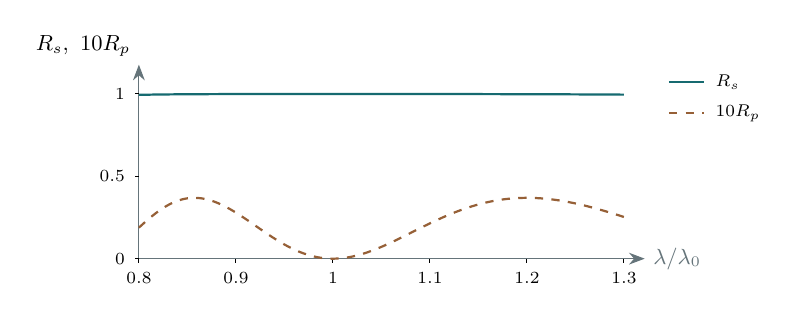
\begin{tikzpicture}[scale=.88,transform shape]
\draw[axis] (0,0.0)--(7.3,0.0) node[right] {$\lambda/\lambda_0$};
\draw[axis] (0,0)--(0,2.8);
\node[above left] at (0,2.8) {$R_s,\ 10R_p$};
\draw[thin] (0.000000,0.0)--(0.000000,-0.06);\node[below,font=\scriptsize] at (0.000000,-0.08) {$ 0.8 $};
\draw[thin] (1.400000,0.0)--(1.400000,-0.06);\node[below,font=\scriptsize] at (1.400000,-0.08) {$ 0.9 $};
\draw[thin] (2.800000,0.0)--(2.800000,-0.06);\node[below,font=\scriptsize] at (2.800000,-0.08) {$ 1 $};
\draw[thin] (4.200000,0.0)--(4.200000,-0.06);\node[below,font=\scriptsize] at (4.200000,-0.08) {$ 1.1 $};
\draw[thin] (5.600000,0.0)--(5.600000,-0.06);\node[below,font=\scriptsize] at (5.600000,-0.08) {$ 1.2 $};
\draw[thin] (7.000000,0.0)--(7.000000,-0.06);\node[below,font=\scriptsize] at (7.000000,-0.08) {$ 1.3 $};
\draw[thin] (0,0.000000)--(-.06,0.000000);\node[left,font=\scriptsize] at (-.08,0.000000) {$ 0 $};
\draw[thin] (0,1.190476)--(-.06,1.190476);\node[left,font=\scriptsize] at (-.08,1.190476) {$ 0.5 $};
\draw[thin] (0,2.380952)--(-.06,2.380952);\node[left,font=\scriptsize] at (-.08,2.380952) {$ 1 $};
\draw[thick,color=accent] plot coordinates {(0.0000000,2.3638414) (0.0291667,2.3645001) (0.0583333,2.3651193) (0.0875000,2.3657020) (0.1166667,2.3662509) (0.1458333,2.3667682) (0.1750000,2.3672563) (0.2041667,2.3677171) (0.2333333,2.3681525) (0.2625000,2.3685643) (0.2916667,2.3689539) (0.3208333,2.3693229) (0.3500000,2.3696726) (0.3791667,2.3700042) (0.4083333,2.3703189) (0.4375000,2.3706176) (0.4666667,2.3709015) (0.4958333,2.3711713) (0.5250000,2.3714280) (0.5541667,2.3716722) (0.5833333,2.3719048) (0.6125000,2.3721264) (0.6416667,2.3723376) (0.6708333,2.3725390) (0.7000000,2.3727311) (0.7291667,2.3729145) (0.7583333,2.3730897) (0.7875000,2.3732570) (0.8166667,2.3734168) (0.8458333,2.3735697) (0.8750000,2.3737158) (0.9041667,2.3738557) (0.9333333,2.3739895) (0.9625000,2.3741176) (0.9916667,2.3742402) (1.0208333,2.3743577) (1.0500000,2.3744702) (1.0791667,2.3745781) (1.1083333,2.3746815) (1.1375000,2.3747806) (1.1666667,2.3748756) (1.1958333,2.3749667) (1.2250000,2.3750541) (1.2541667,2.3751379) (1.2833333,2.3752183) (1.3125000,2.3752955) (1.3416667,2.3753695) (1.3708333,2.3754406) (1.4000000,2.3755087) (1.4291667,2.3755741) (1.4583333,2.3756369) (1.4875000,2.3756971) (1.5166667,2.3757548) (1.5458333,2.3758102) (1.5750000,2.3758633) (1.6041667,2.3759143) (1.6333333,2.3759631) (1.6625000,2.3760099) (1.6916667,2.3760548) (1.7208333,2.3760977) (1.7500000,2.3761389) (1.7791667,2.3761783) (1.8083333,2.3762159) (1.8375000,2.3762520) (1.8666667,2.3762864) (1.8958333,2.3763193) (1.9250000,2.3763507) (1.9541667,2.3763806) (1.9833333,2.3764092) (2.0125000,2.3764363) (2.0416667,2.3764622) (2.0708333,2.3764867) (2.1000000,2.3765100) (2.1291667,2.3765321) (2.1583333,2.3765529) (2.1875000,2.3765727) (2.2166667,2.3765912) (2.2458333,2.3766087) (2.2750000,2.3766251) (2.3041667,2.3766405) (2.3333333,2.3766548) (2.3625000,2.3766682) (2.3916667,2.3766805) (2.4208333,2.3766919) (2.4500000,2.3767024) (2.4791667,2.3767119) (2.5083333,2.3767205) (2.5375000,2.3767283) (2.5666667,2.3767351) (2.5958333,2.3767411) (2.6250000,2.3767463) (2.6541667,2.3767506) (2.6833333,2.3767542) (2.7125000,2.3767569) (2.7416667,2.3767588) (2.7708333,2.3767600) (2.8000000,2.3767603) (2.8291667,2.3767600) (2.8583333,2.3767588) (2.8875000,2.3767570) (2.9166667,2.3767544) (2.9458333,2.3767510) (2.9750000,2.3767470) (3.0041667,2.3767422) (3.0333333,2.3767368) (3.0625000,2.3767306) (3.0916667,2.3767237) (3.1208333,2.3767162) (3.1500000,2.3767079) (3.1791667,2.3766990) (3.2083333,2.3766894) (3.2375000,2.3766791) (3.2666667,2.3766682) (3.2958333,2.3766566) (3.3250000,2.3766443) (3.3541667,2.3766313) (3.3833333,2.3766177) (3.4125000,2.3766034) (3.4416667,2.3765885) (3.4708333,2.3765729) (3.5000000,2.3765566) (3.5291667,2.3765397) (3.5583333,2.3765221) (3.5875000,2.3765038) (3.6166667,2.3764849) (3.6458333,2.3764653) (3.6750000,2.3764451) (3.7041667,2.3764242) (3.7333333,2.3764026) (3.7625000,2.3763803) (3.7916667,2.3763574) (3.8208333,2.3763338) (3.8500000,2.3763095) (3.8791667,2.3762845) (3.9083333,2.3762588) (3.9375000,2.3762324) (3.9666667,2.3762054) (3.9958333,2.3761776) (4.0250000,2.3761491) (4.0541667,2.3761199) (4.0833333,2.3760900) (4.1125000,2.3760594) (4.1416667,2.3760280) (4.1708333,2.3759959) (4.2000000,2.3759631) (4.2291667,2.3759295) (4.2583333,2.3758952) (4.2875000,2.3758601) (4.3166667,2.3758242) (4.3458333,2.3757876) (4.3750000,2.3757502) (4.4041667,2.3757120) (4.4333333,2.3756729) (4.4625000,2.3756331) (4.4916667,2.3755925) (4.5208333,2.3755510) (4.5500000,2.3755087) (4.5791667,2.3754656) (4.6083333,2.3754216) (4.6375000,2.3753767) (4.6666667,2.3753309) (4.6958333,2.3752843) (4.7250000,2.3752368) (4.7541667,2.3751883) (4.7833333,2.3751390) (4.8125000,2.3750887) (4.8416667,2.3750375) (4.8708333,2.3749853) (4.9000000,2.3749321) (4.9291667,2.3748780) (4.9583333,2.3748228) (4.9875000,2.3747667) (5.0166667,2.3747095) (5.0458333,2.3746513) (5.0750000,2.3745920) (5.1041667,2.3745317) (5.1333333,2.3744702) (5.1625000,2.3744077) (5.1916667,2.3743441) (5.2208333,2.3742793) (5.2500000,2.3742134) (5.2791667,2.3741463) (5.3083333,2.3740781) (5.3375000,2.3740086) (5.3666667,2.3739380) (5.3958333,2.3738660) (5.4250000,2.3737929) (5.4541667,2.3737184) (5.4833333,2.3736427) (5.5125000,2.3735656) (5.5416667,2.3734872) (5.5708333,2.3734075) (5.6000000,2.3733264) (5.6291667,2.3732438) (5.6583333,2.3731599) (5.6875000,2.3730745) (5.7166667,2.3729876) (5.7458333,2.3728993) (5.7750000,2.3728094) (5.8041667,2.3727180) (5.8333333,2.3726250) (5.8625000,2.3725304) (5.8916667,2.3724342) (5.9208333,2.3723364) (5.9500000,2.3722369) (5.9791667,2.3721357) (6.0083333,2.3720327) (6.0375000,2.3719280) (6.0666667,2.3718215) (6.0958333,2.3717132) (6.1250000,2.3716031) (6.1541667,2.3714910) (6.1833333,2.3713771) (6.2125000,2.3712612) (6.2416667,2.3711433) (6.2708333,2.3710234) (6.3000000,2.3709015) (6.3291667,2.3707775) (6.3583333,2.3706513) (6.3875000,2.3705230) (6.4166667,2.3703925) (6.4458333,2.3702598) (6.4750000,2.3701248) (6.5041667,2.3699875) (6.5333333,2.3698478) (6.5625000,2.3697057) (6.5916667,2.3695612) (6.6208333,2.3694143) (6.6500000,2.3692647) (6.6791667,2.3691127) (6.7083333,2.3689580) (6.7375000,2.3688006) (6.7666667,2.3686405) (6.7958333,2.3684777) (6.8250000,2.3683121) (6.8541667,2.3681436) (6.8833333,2.3679721) (6.9125000,2.3677978) (6.9416667,2.3676204) (6.9708333,2.3674399) (7.0000000,2.3672563)};
\draw[thick,color=accent] (7.65,2.55)--(8.15,2.55);\node[right,font=\scriptsize] at (8.2,2.55) {$R_s$};
\draw[thick,dashed,color=warm] plot coordinates {(0.0000000,0.4471258) (0.0291667,0.4739284) (0.0583333,0.5004321) (0.0875000,0.5265442) (0.1166667,0.5521765) (0.1458333,0.5772454) (0.1750000,0.6016721) (0.2041667,0.6253824) (0.2333333,0.6483072) (0.2625000,0.6703825) (0.2916667,0.6915487) (0.3208333,0.7117517) (0.3500000,0.7309419) (0.3791667,0.7490746) (0.4083333,0.7661101) (0.4375000,0.7820132) (0.4666667,0.7967532) (0.4958333,0.8103042) (0.5250000,0.8226444) (0.5541667,0.8337565) (0.5833333,0.8436271) (0.6125000,0.8522471) (0.6416667,0.8596111) (0.6708333,0.8657174) (0.7000000,0.8705681) (0.7291667,0.8741684) (0.7583333,0.8765273) (0.7875000,0.8776565) (0.8166667,0.8775711) (0.8458333,0.8762887) (0.8750000,0.8738299) (0.9041667,0.8702178) (0.9333333,0.8654781) (0.9625000,0.8596384) (0.9916667,0.8527289) (1.0208333,0.8447815) (1.0500000,0.8358303) (1.0791667,0.8259107) (1.1083333,0.8150602) (1.1375000,0.8033175) (1.1666667,0.7907227) (1.1958333,0.7773171) (1.2250000,0.7631432) (1.2541667,0.7482444) (1.2833333,0.7326650) (1.3125000,0.7164500) (1.3416667,0.6996449) (1.3708333,0.6822960) (1.4000000,0.6644497) (1.4291667,0.6461528) (1.4583333,0.6274523) (1.4875000,0.6083951) (1.5166667,0.5890284) (1.5458333,0.5693987) (1.5750000,0.5495529) (1.6041667,0.5295370) (1.6333333,0.5093970) (1.6625000,0.4891780) (1.6916667,0.4689248) (1.7208333,0.4486813) (1.7500000,0.4284907) (1.7791667,0.4083954) (1.8083333,0.3884367) (1.8375000,0.3686550) (1.8666667,0.3490897) (1.8958333,0.3297789) (1.9250000,0.3107597) (1.9541667,0.2920677) (1.9833333,0.2737374) (2.0125000,0.2558019) (2.0416667,0.2382928) (2.0708333,0.2212404) (2.1000000,0.2046734) (2.1291667,0.1886191) (2.1583333,0.1731032) (2.1875000,0.1581499) (2.2166667,0.1437816) (2.2458333,0.1300195) (2.2750000,0.1168829) (2.3041667,0.1043896) (2.3333333,0.0925558) (2.3625000,0.0813959) (2.3916667,0.0709229) (2.4208333,0.0611482) (2.4500000,0.0520816) (2.4791667,0.0437312) (2.5083333,0.0361037) (2.5375000,0.0292042) (2.5666667,0.0230363) (2.5958333,0.0176023) (2.6250000,0.0129028) (2.6541667,0.0089372) (2.6833333,0.0057033) (2.7125000,0.0031980) (2.7416667,0.0014164) (2.7708333,0.0003528) (2.8000000,0.0000000) (2.8291667,0.0003499) (2.8583333,0.0013930) (2.8875000,0.0031191) (2.9166667,0.0055168) (2.9458333,0.0085737) (2.9750000,0.0122767) (3.0041667,0.0166116) (3.0333333,0.0215637) (3.0625000,0.0271174) (3.0916667,0.0332563) (3.1208333,0.0399636) (3.1500000,0.0472218) (3.1791667,0.0550128) (3.2083333,0.0633182) (3.2375000,0.0721190) (3.2666667,0.0813959) (3.2958333,0.0911292) (3.3250000,0.1012990) (3.3541667,0.1118851) (3.3833333,0.1228671) (3.4125000,0.1342245) (3.4416667,0.1459366) (3.4708333,0.1579826) (3.5000000,0.1703419) (3.5291667,0.1829936) (3.5583333,0.1959170) (3.5875000,0.2090915) (3.6166667,0.2224965) (3.6458333,0.2361117) (3.6750000,0.2499166) (3.7041667,0.2638914) (3.7333333,0.2780161) (3.7625000,0.2922712) (3.7916667,0.3066373) (3.8208333,0.3210955) (3.8500000,0.3356269) (3.8791667,0.3502132) (3.9083333,0.3648364) (3.9375000,0.3794787) (3.9666667,0.3941228) (3.9958333,0.4087519) (4.0250000,0.4233493) (4.0541667,0.4378989) (4.0833333,0.4523852) (4.1125000,0.4667927) (4.1416667,0.4811067) (4.1708333,0.4953128) (4.2000000,0.5093970) (4.2291667,0.5233459) (4.2583333,0.5371463) (4.2875000,0.5507859) (4.3166667,0.5642523) (4.3458333,0.5775340) (4.3750000,0.5906198) (4.4041667,0.6034989) (4.4333333,0.6161610) (4.4625000,0.6285963) (4.4916667,0.6407954) (4.5208333,0.6527493) (4.5500000,0.6644497) (4.5791667,0.6758884) (4.6083333,0.6870578) (4.6375000,0.6979507) (4.6666667,0.7085604) (4.6958333,0.7188806) (4.7250000,0.7289052) (4.7541667,0.7386288) (4.7833333,0.7480464) (4.8125000,0.7571530) (4.8416667,0.7659445) (4.8708333,0.7744168) (4.9000000,0.7825664) (4.9291667,0.7903900) (4.9583333,0.7978847) (4.9875000,0.8050482) (5.0166667,0.8118780) (5.0458333,0.8183726) (5.0750000,0.8245302) (5.1041667,0.8303497) (5.1333333,0.8358303) (5.1625000,0.8409712) (5.1916667,0.8457723) (5.2208333,0.8502336) (5.2500000,0.8543552) (5.2791667,0.8581377) (5.3083333,0.8615820) (5.3375000,0.8646891) (5.3666667,0.8674602) (5.3958333,0.8698969) (5.4250000,0.8720011) (5.4541667,0.8737746) (5.4833333,0.8752197) (5.5125000,0.8763389) (5.5416667,0.8771347) (5.5708333,0.8776099) (5.6000000,0.8777677) (5.6291667,0.8776110) (5.6583333,0.8771434) (5.6875000,0.8763683) (5.7166667,0.8752895) (5.7458333,0.8739107) (5.7750000,0.8722360) (5.8041667,0.8702694) (5.8333333,0.8680153) (5.8625000,0.8654781) (5.8916667,0.8626622) (5.9208333,0.8595723) (5.9500000,0.8562131) (5.9791667,0.8525895) (6.0083333,0.8487064) (6.0375000,0.8445689) (6.0666667,0.8401821) (6.0958333,0.8355512) (6.1250000,0.8306815) (6.1541667,0.8255783) (6.1833333,0.8202472) (6.2125000,0.8146935) (6.2416667,0.8089229) (6.2708333,0.8029409) (6.3000000,0.7967532) (6.3291667,0.7903655) (6.3583333,0.7837835) (6.3875000,0.7770130) (6.4166667,0.7700598) (6.4458333,0.7629298) (6.4750000,0.7556287) (6.5041667,0.7481625) (6.5333333,0.7405370) (6.5625000,0.7327581) (6.5916667,0.7248318) (6.6208333,0.7167639) (6.6500000,0.7085604) (6.6791667,0.7002271) (6.7083333,0.6917700) (6.7375000,0.6831949) (6.7666667,0.6745077) (6.7958333,0.6657142) (6.8250000,0.6568204) (6.8541667,0.6478319) (6.8833333,0.6387546) (6.9125000,0.6295943) (6.9416667,0.6203566) (6.9708333,0.6110473) (7.0000000,0.6016721)};
\draw[thick,dashed,color=warm] (7.65,2.0999999999999996)--(8.15,2.0999999999999996);\node[right,font=\scriptsize] at (8.2,2.0999999999999996) {$10R_p$};
\end{tikzpicture}
\figcaption{解图光4.3C\quad 固定三对设计膜的波长响应，$p$曲线放大十倍}
\end{minipage}\end{center}

\textbf{入射角误差也同时改变两种条件。}固定棱镜折射率和物理膜厚，改变棱镜内角$\vartheta$后，切向量改为$n\sin\vartheta$，$\cos\theta_H,\cos\theta_L$及两层相位都随之改变。既可能偏离内部$p$布儒斯特条件，也可能偏离四分之一波条件，不能只给某层光程乘一个共同的$\cos\vartheta$。图D对$43^\circ$到$47^\circ$的角域逐层重算，用$R_s$和$5R_p$比较角容差；无吸收和无全反射仍须逐层核查。

例如内角改为$44^\circ$或$46^\circ$时，$p$反射率分别约为0.02930和0.03672，而$s$反射率仍接近0.998；两个偏振指标对角度的敏感程度不同。
\begin{center}\begin{minipage}{.98\linewidth}\centering
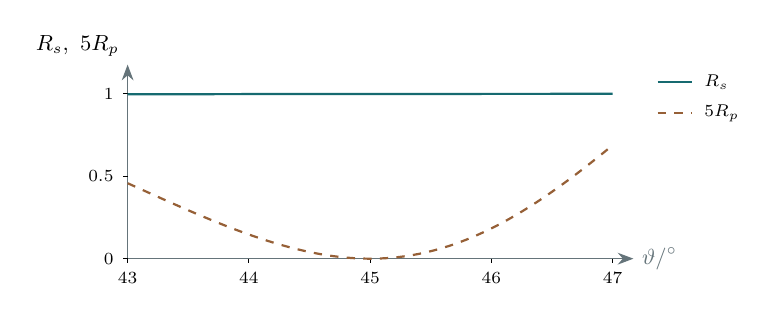
\begin{tikzpicture}[scale=.88,transform shape]
\draw[axis] (0,0.0)--(7.3,0.0) node[right] {$\vartheta/^\circ$};
\draw[axis] (0,0)--(0,2.8);
\node[above left] at (0,2.8) {$R_s,\ 5R_p$};
\draw[thin] (0.000000,0.0)--(0.000000,-0.06);\node[below,font=\scriptsize] at (0.000000,-0.08) {$ 43 $};
\draw[thin] (1.750000,0.0)--(1.750000,-0.06);\node[below,font=\scriptsize] at (1.750000,-0.08) {$ 44 $};
\draw[thin] (3.500000,0.0)--(3.500000,-0.06);\node[below,font=\scriptsize] at (3.500000,-0.08) {$ 45 $};
\draw[thin] (5.250000,0.0)--(5.250000,-0.06);\node[below,font=\scriptsize] at (5.250000,-0.08) {$ 46 $};
\draw[thin] (7.000000,0.0)--(7.000000,-0.06);\node[below,font=\scriptsize] at (7.000000,-0.08) {$ 47 $};
\draw[thin] (0,0.000000)--(-.06,0.000000);\node[left,font=\scriptsize] at (-.08,0.000000) {$ 0 $};
\draw[thin] (0,1.190476)--(-.06,1.190476);\node[left,font=\scriptsize] at (-.08,1.190476) {$ 0.5 $};
\draw[thin] (0,2.380952)--(-.06,2.380952);\node[left,font=\scriptsize] at (-.08,2.380952) {$ 1 $};
\draw[thick,color=accent] plot coordinates {(0.0000000,2.3722390) (0.0291667,2.3722942) (0.0583333,2.3723491) (0.0875000,2.3724035) (0.1166667,2.3724576) (0.1458333,2.3725113) (0.1750000,2.3725647) (0.2041667,2.3726176) (0.2333333,2.3726702) (0.2625000,2.3727224) (0.2916667,2.3727743) (0.3208333,2.3728257) (0.3500000,2.3728769) (0.3791667,2.3729276) (0.4083333,2.3729780) (0.4375000,2.3730281) (0.4666667,2.3730778) (0.4958333,2.3731271) (0.5250000,2.3731762) (0.5541667,2.3732248) (0.5833333,2.3732732) (0.6125000,2.3733212) (0.6416667,2.3733688) (0.6708333,2.3734162) (0.7000000,2.3734632) (0.7291667,2.3735098) (0.7583333,2.3735562) (0.7875000,2.3736022) (0.8166667,2.3736479) (0.8458333,2.3736933) (0.8750000,2.3737384) (0.9041667,2.3737832) (0.9333333,2.3738276) (0.9625000,2.3738718) (0.9916667,2.3739156) (1.0208333,2.3739592) (1.0500000,2.3740024) (1.0791667,2.3740453) (1.1083333,2.3740880) (1.1375000,2.3741304) (1.1666667,2.3741724) (1.1958333,2.3742142) (1.2250000,2.3742557) (1.2541667,2.3742969) (1.2833333,2.3743378) (1.3125000,2.3743784) (1.3416667,2.3744188) (1.3708333,2.3744589) (1.4000000,2.3744987) (1.4291667,2.3745382) (1.4583333,2.3745775) (1.4875000,2.3746165) (1.5166667,2.3746552) (1.5458333,2.3746937) (1.5750000,2.3747319) (1.6041667,2.3747699) (1.6333333,2.3748076) (1.6625000,2.3748450) (1.6916667,2.3748822) (1.7208333,2.3749191) (1.7500000,2.3749558) (1.7791667,2.3749922) (1.8083333,2.3750284) (1.8375000,2.3750643) (1.8666667,2.3751000) (1.8958333,2.3751354) (1.9250000,2.3751707) (1.9541667,2.3752056) (1.9833333,2.3752404) (2.0125000,2.3752749) (2.0416667,2.3753091) (2.0708333,2.3753432) (2.1000000,2.3753770) (2.1291667,2.3754105) (2.1583333,2.3754439) (2.1875000,2.3754770) (2.2166667,2.3755099) (2.2458333,2.3755426) (2.2750000,2.3755751) (2.3041667,2.3756073) (2.3333333,2.3756394) (2.3625000,2.3756712) (2.3916667,2.3757028) (2.4208333,2.3757342) (2.4500000,2.3757654) (2.4791667,2.3757964) (2.5083333,2.3758271) (2.5375000,2.3758577) (2.5666667,2.3758880) (2.5958333,2.3759182) (2.6250000,2.3759482) (2.6541667,2.3759779) (2.6833333,2.3760075) (2.7125000,2.3760368) (2.7416667,2.3760660) (2.7708333,2.3760950) (2.8000000,2.3761238) (2.8291667,2.3761524) (2.8583333,2.3761808) (2.8875000,2.3762090) (2.9166667,2.3762370) (2.9458333,2.3762648) (2.9750000,2.3762925) (3.0041667,2.3763200) (3.0333333,2.3763473) (3.0625000,2.3763744) (3.0916667,2.3764013) (3.1208333,2.3764281) (3.1500000,2.3764547) (3.1791667,2.3764811) (3.2083333,2.3765073) (3.2375000,2.3765334) (3.2666667,2.3765592) (3.2958333,2.3765850) (3.3250000,2.3766105) (3.3541667,2.3766359) (3.3833333,2.3766611) (3.4125000,2.3766862) (3.4416667,2.3767111) (3.4708333,2.3767358) (3.5000000,2.3767603) (3.5291667,2.3767848) (3.5583333,2.3768090) (3.5875000,2.3768331) (3.6166667,2.3768570) (3.6458333,2.3768808) (3.6750000,2.3769044) (3.7041667,2.3769279) (3.7333333,2.3769512) (3.7625000,2.3769743) (3.7916667,2.3769974) (3.8208333,2.3770202) (3.8500000,2.3770429) (3.8791667,2.3770655) (3.9083333,2.3770879) (3.9375000,2.3771102) (3.9666667,2.3771323) (3.9958333,2.3771543) (4.0250000,2.3771762) (4.0541667,2.3771979) (4.0833333,2.3772194) (4.1125000,2.3772409) (4.1416667,2.3772621) (4.1708333,2.3772833) (4.2000000,2.3773043) (4.2291667,2.3773252) (4.2583333,2.3773459) (4.2875000,2.3773666) (4.3166667,2.3773870) (4.3458333,2.3774074) (4.3750000,2.3774276) (4.4041667,2.3774477) (4.4333333,2.3774677) (4.4625000,2.3774875) (4.4916667,2.3775072) (4.5208333,2.3775268) (4.5500000,2.3775462) (4.5791667,2.3775656) (4.6083333,2.3775848) (4.6375000,2.3776039) (4.6666667,2.3776228) (4.6958333,2.3776417) (4.7250000,2.3776604) (4.7541667,2.3776790) (4.7833333,2.3776975) (4.8125000,2.3777158) (4.8416667,2.3777341) (4.8708333,2.3777522) (4.9000000,2.3777703) (4.9291667,2.3777882) (4.9583333,2.3778060) (4.9875000,2.3778236) (5.0166667,2.3778412) (5.0458333,2.3778587) (5.0750000,2.3778760) (5.1041667,2.3778933) (5.1333333,2.3779104) (5.1625000,2.3779274) (5.1916667,2.3779443) (5.2208333,2.3779611) (5.2500000,2.3779778) (5.2791667,2.3779944) (5.3083333,2.3780109) (5.3375000,2.3780273) (5.3666667,2.3780436) (5.3958333,2.3780598) (5.4250000,2.3780759) (5.4541667,2.3780919) (5.4833333,2.3781077) (5.5125000,2.3781235) (5.5416667,2.3781392) (5.5708333,2.3781548) (5.6000000,2.3781703) (5.6291667,2.3781857) (5.6583333,2.3782010) (5.6875000,2.3782162) (5.7166667,2.3782313) (5.7458333,2.3782463) (5.7750000,2.3782612) (5.8041667,2.3782760) (5.8333333,2.3782908) (5.8625000,2.3783054) (5.8916667,2.3783200) (5.9208333,2.3783344) (5.9500000,2.3783488) (5.9791667,2.3783631) (6.0083333,2.3783773) (6.0375000,2.3783914) (6.0666667,2.3784054) (6.0958333,2.3784193) (6.1250000,2.3784332) (6.1541667,2.3784470) (6.1833333,2.3784606) (6.2125000,2.3784742) (6.2416667,2.3784877) (6.2708333,2.3785012) (6.3000000,2.3785145) (6.3291667,2.3785278) (6.3583333,2.3785409) (6.3875000,2.3785540) (6.4166667,2.3785671) (6.4458333,2.3785800) (6.4750000,2.3785929) (6.5041667,2.3786056) (6.5333333,2.3786184) (6.5625000,2.3786310) (6.5916667,2.3786435) (6.6208333,2.3786560) (6.6500000,2.3786684) (6.6791667,2.3786807) (6.7083333,2.3786930) (6.7375000,2.3787051) (6.7666667,2.3787172) (6.7958333,2.3787292) (6.8250000,2.3787412) (6.8541667,2.3787531) (6.8833333,2.3787649) (6.9125000,2.3787766) (6.9416667,2.3787883) (6.9708333,2.3787999) (7.0000000,2.3788114)};
\draw[thick,color=accent] (7.65,2.55)--(8.15,2.55);\node[right,font=\scriptsize] at (8.2,2.55) {$R_s$};
\draw[thick,dashed,color=warm] plot coordinates {(0.0000000,1.0888272) (0.0291667,1.0756732) (0.0583333,1.0625148) (0.0875000,1.0493535) (0.1166667,1.0361906) (0.1458333,1.0230277) (0.1750000,1.0098661) (0.2041667,0.9967074) (0.2333333,0.9835531) (0.2625000,0.9704047) (0.2916667,0.9572637) (0.3208333,0.9441317) (0.3500000,0.9310103) (0.3791667,0.9179010) (0.4083333,0.9048055) (0.4375000,0.8917254) (0.4666667,0.8786623) (0.4958333,0.8656180) (0.5250000,0.8525940) (0.5541667,0.8395921) (0.5833333,0.8266141) (0.6125000,0.8136616) (0.6416667,0.8007364) (0.6708333,0.7878403) (0.7000000,0.7749750) (0.7291667,0.7621425) (0.7583333,0.7493444) (0.7875000,0.7365826) (0.8166667,0.7238591) (0.8458333,0.7111756) (0.8750000,0.6985341) (0.9041667,0.6859364) (0.9333333,0.6733845) (0.9625000,0.6608804) (0.9916667,0.6484259) (1.0208333,0.6360231) (1.0500000,0.6236739) (1.0791667,0.6113804) (1.1083333,0.5991445) (1.1375000,0.5869684) (1.1666667,0.5748539) (1.1958333,0.5628032) (1.2250000,0.5508184) (1.2541667,0.5389016) (1.2833333,0.5270548) (1.3125000,0.5152801) (1.3416667,0.5035798) (1.3708333,0.4919558) (1.4000000,0.4804105) (1.4291667,0.4689458) (1.4583333,0.4575641) (1.4875000,0.4462674) (1.5166667,0.4350580) (1.5458333,0.4239381) (1.5750000,0.4129099) (1.6041667,0.4019756) (1.6333333,0.3911374) (1.6625000,0.3803976) (1.6916667,0.3697584) (1.7208333,0.3592221) (1.7500000,0.3487909) (1.7791667,0.3384671) (1.8083333,0.3282530) (1.8375000,0.3181508) (1.8666667,0.3081628) (1.8958333,0.2982913) (1.9250000,0.2885386) (1.9541667,0.2789070) (1.9833333,0.2693987) (2.0125000,0.2600161) (2.0416667,0.2507615) (2.0708333,0.2416371) (2.1000000,0.2326453) (2.1291667,0.2237883) (2.1583333,0.2150685) (2.1875000,0.2064881) (2.2166667,0.1980493) (2.2458333,0.1897546) (2.2750000,0.1816062) (2.3041667,0.1736063) (2.3333333,0.1657572) (2.3625000,0.1580613) (2.3916667,0.1505206) (2.4208333,0.1431376) (2.4500000,0.1359144) (2.4791667,0.1288532) (2.5083333,0.1219563) (2.5375000,0.1152259) (2.5666667,0.1086642) (2.5958333,0.1022733) (2.6250000,0.0960556) (2.6541667,0.0900130) (2.6833333,0.0841477) (2.7125000,0.0784619) (2.7416667,0.0729577) (2.7708333,0.0676372) (2.8000000,0.0625025) (2.8291667,0.0575555) (2.8583333,0.0527984) (2.8875000,0.0482332) (2.9166667,0.0438619) (2.9458333,0.0396864) (2.9750000,0.0357087) (3.0041667,0.0319307) (3.0333333,0.0283543) (3.0625000,0.0249815) (3.0916667,0.0218140) (3.1208333,0.0188537) (3.1500000,0.0161023) (3.1791667,0.0135618) (3.2083333,0.0112337) (3.2375000,0.0091198) (3.2666667,0.0072218) (3.2958333,0.0055413) (3.3250000,0.0040800) (3.3541667,0.0028393) (3.3833333,0.0018210) (3.4125000,0.0010264) (3.4416667,0.0004571) (3.4708333,0.0001145) (3.5000000,0.0000000) (3.5291667,0.0001150) (3.5583333,0.0004607) (3.5875000,0.0010385) (3.6166667,0.0018497) (3.6458333,0.0028954) (3.6750000,0.0041768) (3.7041667,0.0056951) (3.7333333,0.0074512) (3.7625000,0.0094463) (3.7916667,0.0116814) (3.8208333,0.0141573) (3.8500000,0.0168750) (3.8791667,0.0198354) (3.9083333,0.0230393) (3.9375000,0.0264874) (3.9666667,0.0301805) (3.9958333,0.0341192) (4.0250000,0.0383042) (4.0541667,0.0427361) (4.0833333,0.0474153) (4.1125000,0.0523423) (4.1416667,0.0575176) (4.1708333,0.0629416) (4.2000000,0.0686145) (4.2291667,0.0745367) (4.2583333,0.0807084) (4.2875000,0.0871298) (4.3166667,0.0938010) (4.3458333,0.1007220) (4.3750000,0.1078929) (4.4041667,0.1153136) (4.4333333,0.1229841) (4.4625000,0.1309043) (4.4916667,0.1390739) (4.5208333,0.1474927) (4.5500000,0.1561604) (4.5791667,0.1650766) (4.6083333,0.1742410) (4.6375000,0.1836532) (4.6666667,0.1933125) (4.6958333,0.2032185) (4.7250000,0.2133705) (4.7541667,0.2237679) (4.7833333,0.2344100) (4.8125000,0.2452960) (4.8416667,0.2564250) (4.8708333,0.2677963) (4.9000000,0.2794088) (4.9291667,0.2912617) (4.9583333,0.3033539) (4.9875000,0.3156843) (5.0166667,0.3282518) (5.0458333,0.3410552) (5.0750000,0.3540933) (5.1041667,0.3673649) (5.1333333,0.3808686) (5.1625000,0.3946030) (5.1916667,0.4085668) (5.2208333,0.4227584) (5.2500000,0.4371764) (5.2791667,0.4518192) (5.3083333,0.4666852) (5.3375000,0.4817728) (5.3666667,0.4970802) (5.3958333,0.5126058) (5.4250000,0.5283477) (5.4541667,0.5443042) (5.4833333,0.5604733) (5.5125000,0.5768533) (5.5416667,0.5934420) (5.5708333,0.6102377) (5.6000000,0.6272381) (5.6291667,0.6444414) (5.6583333,0.6618453) (5.6875000,0.6794478) (5.7166667,0.6972466) (5.7458333,0.7152397) (5.7750000,0.7334247) (5.8041667,0.7517993) (5.8333333,0.7703614) (5.8625000,0.7891085) (5.8916667,0.8080382) (5.9208333,0.8271483) (5.9500000,0.8464362) (5.9791667,0.8658995) (6.0083333,0.8855358) (6.0375000,0.9053425) (6.0666667,0.9253171) (6.0958333,0.9454570) (6.1250000,0.9657598) (6.1541667,0.9862227) (6.1833333,1.0068431) (6.2125000,1.0276185) (6.2416667,1.0485461) (6.2708333,1.0696234) (6.3000000,1.0908475) (6.3291667,1.1122157) (6.3583333,1.1337254) (6.3875000,1.1553738) (6.4166667,1.1771582) (6.4458333,1.1990757) (6.4750000,1.2211235) (6.5041667,1.2432990) (6.5333333,1.2655992) (6.5625000,1.2880215) (6.5916667,1.3105628) (6.6208333,1.3332205) (6.6500000,1.3559916) (6.6791667,1.3788734) (6.7083333,1.4018630) (6.7375000,1.4249575) (6.7666667,1.4481540) (6.7958333,1.4714498) (6.8250000,1.4948420) (6.8541667,1.5183276) (6.8833333,1.5419039) (6.9125000,1.5655680) (6.9416667,1.5893170) (6.9708333,1.6131480) (7.0000000,1.6370583)};
\draw[thick,dashed,color=warm] (7.65,2.0999999999999996)--(8.15,2.0999999999999996);\node[right,font=\scriptsize] at (8.2,2.0999999999999996) {$5R_p$};
\end{tikzpicture}
\figcaption{解图光4.3D\quad 固定膜与材料，角度改变时逐层重算}
\end{minipage}\end{center}

上述结果适用于所列终止结构和固定材料常数。外表面反射、胶层、材料色散和吸收会改变实际效率与消光比。它们若被忽略，应保留为建模条件；若要纳入，须增加相应界面或复折射率，不把“内部$s$反射相长”直接等同于器件所有端口都达到理想分束。


\Needspace{13\baselineskip}

\pdfbookmark[2]{第 4 题 反射与折射后的偏振方向}{q4}

\section*{第 4 题\quad 反射与折射后的偏振方向}\label{q:4}

线偏振光从折射率$n_1$的透明介质射向折射率$n_2$的透明介质，入射角为$\theta_1$，电矢量与入射面夹角为$\alpha$。求反射光、折射光的偏振方向，并讨论布儒斯特入射、法向入射及全反射。

\begin{center}\begin{minipage}{.98\linewidth}\centering
\begin{tikzpicture}[scale=.9,transform shape]
\draw[object] (-3.10000,0.00000)--(3.50000,0.00000);\draw[guide] (0.00000,-2.50000)--(0.00000,2.70000);\fill (0.00000,0.00000) circle(.035);\node[above right] at (0.00000,0.00000) {$O$};\draw[motion] (-1.76777,1.76777)--(0.00000,0.00000);
\draw[motion] (0.00000,0.00000)--(1.76777,1.76777);\draw[motion] (0.00000,0.00000)--(1.17851,-2.20479);\node[right] at (-2.90000,1.50000) {$n_1$};\node[right] at (-2.90000,-1.50000) {$n_2$};\node[left] at (-0.50000,1.00000) {$\theta_i$};\node[right] at (0.55000,1.10000) {$\theta_r$};\node[right] at (0.42000,-1.00000) {$\theta_t$};\node[above] at (-2.00000,2.40000) {入射 $E_p,E_s$};\node[above] at (2.70000,2.20000) {反射};
\end{tikzpicture}
\figcaption{图光4.4\quad 界面三束光与共同入射面}
\end{minipage}\end{center}

\Needspace{6\baselineskip}\subsection*{解答}


\textbf{坐标与两种偏振分量。}取界面为$z=0$、入射面为$xz$面，介质1在$z<0$，共同$s$轴沿$+y$。三束波的传播方向为
\[
\hat{\boldsymbol k}_i=(\sin\theta_1,0,\cos\theta_1),\quad
\hat{\boldsymbol k}_r=(\sin\theta_1,0,-\cos\theta_1),\quad
\hat{\boldsymbol k}_t=(\sin\theta_2,0,\cos\theta_2).
\]
按图A定义$\boldsymbol p_j=\boldsymbol s\times\hat{\boldsymbol k}_j$，排列顺序采用$(p,s)$。入射Jones向量为$E_0(\cos\alpha,\sin\alpha)$。这两个分量来自同一线偏振场，具有固定相位关系。

图A下方取$n_1=1,n_2=1.50,\theta_1=45^\circ,\alpha=45^\circ$示意三个场方向，每束箭头分别归一；上方给出一般分量关系。
\begin{center}\begin{minipage}{.98\linewidth}\centering
\begin{tikzpicture}[scale=.8,transform shape]
\node[above right] at (0.00000,0.40000) {步骤};\node[above right] at (3.40000,0.40000) {分量或关系};\node[above right] at (7.40000,0.40000) {说明};\draw[thin] (-0.20000,0.10000)--(10.80000,0.10000);\node[above right] at (0.00000,-0.48000) {入射};\node[above right] at (3.40000,-0.48000) {$(\cos\alpha,\sin\alpha)$};\node[above right] at (7.40000,-0.48000) {};\node[above right] at (0.00000,-1.11000) {反射};\node[above right] at (3.40000,-1.11000) {$(r_p\cos\alpha,r_s\sin\alpha)$};\node[above right] at (7.40000,-1.11000) {局部 $p_r,s$};\node[above right] at (0.00000,-1.74000) {透射};\node[above right] at (3.40000,-1.74000) {$(t_p\cos\alpha,t_s\sin\alpha)$};\node[above right] at (7.40000,-1.74000) {局部 $p_t,s$};\node[above] at (4.80000,-2.50000) {局部基矢 $\boldsymbol p_j=\boldsymbol s\times\hat{\boldsymbol k}_j$};\begin{scope}[shift={(1.00000,-5.00000)}]
\draw[axis] (-1.05000,0.00000)--(1.05000,0.00000);\draw[axis] (0.00000,-1.05000)--(0.00000,1.05000);\node[below right] at (1.05000,0.00000) {$p_i$};\node[above right] at (0.00000,1.05000) {$s$};\draw[force] (-0.70711,-0.70711)--(0.70711,0.70711);\node[above right] at (0.79903,0.79903) {$E$};\node[above] at (0.00000,1.70000) {入射};
\end{scope}\begin{scope}[shift={(5.00000,-5.00000)}]
\draw[axis] (-1.05000,0.00000)--(1.05000,0.00000);\draw[axis] (0.00000,-1.05000)--(0.00000,1.05000);\node[below right] at (1.05000,0.00000) {$p_r$};\node[above right] at (0.00000,1.05000) {$s$};\draw[force] (-0.29028,0.95694)--(0.29028,-0.95694);\node[below right] at (0.32801,-1.08135) {$E$};\node[above] at (0.00000,1.70000) {反射};
\end{scope}\begin{scope}[shift={(9.00000,-5.00000)}]
\draw[axis] (-1.05000,0.00000)--(1.05000,0.00000);\draw[axis] (0.00000,-1.05000)--(0.00000,1.05000);\node[below right] at (1.05000,0.00000) {$p_t$};\node[above right] at (0.00000,1.05000) {$s$};\draw[force] (-0.72249,-0.69138)--(0.72249,0.69138);\node[above right] at (0.81641,0.78126) {$E$};\node[above] at (0.00000,1.70000) {透射};
\end{scope}
\end{tikzpicture}
\figcaption{解图光4.4A\quad 按各光束局部基矢作振幅投影}
\end{minipage}\end{center}

\textbf{由界面条件求振幅。}先取透明介质且存在实折射角，$n_1\sin\theta_1=n_2\sin\theta_2$。对$s$分量，切向电、磁场连续分别给
\[
1+r_s=t_s,\qquad n_1\cos\theta_1(1-r_s)=n_2\cos\theta_2t_s.
\]
反射束的局部$p$轴切向投影反向，故$p$分量满足
\[
\cos\theta_1(1-r_p)=\cos\theta_2t_p,\qquad
n_1(1+r_p)=n_2t_p.
\]
分别联立，得到
\[
\begin{aligned}
r_s&=\frac{n_1\cos\theta_1-n_2\cos\theta_2}{n_1\cos\theta_1+n_2\cos\theta_2},&
r_p&=\frac{n_2\cos\theta_1-n_1\cos\theta_2}{n_2\cos\theta_1+n_1\cos\theta_2},\\
t_s&=\frac{2n_1\cos\theta_1}{n_1\cos\theta_1+n_2\cos\theta_2},&
t_p&=\frac{2n_1\cos\theta_1}{n_2\cos\theta_1+n_1\cos\theta_2}.
\end{aligned}
\]
于是反射、折射Jones向量分别为$E_0(r_p\cos\alpha,r_s\sin\alpha)$与$E_0(t_p\cos\alpha,t_s\sin\alpha)$。这些系数为实数，各束的两个分量保持0或$\pi$相位差，输出沿固定直线振动；负系数使相应有向分量反向。

\textbf{振动方位角。}根据图A的局部坐标，非零出射场的有向线轴角为
\[
\alpha_r=\operatorname{atan2}(r_s\sin\alpha,r_p\cos\alpha)\pmod\pi,
\quad
\alpha_t=\operatorname{atan2}(t_s\sin\alpha,t_p\cos\alpha)\pmod\pi.
\]
若题目取电矢量与入射面的锐夹角，则对分量比取绝对值。利用Snell关系化简，可得
\[
\frac{r_s}{r_p}=-\frac{\cos(\theta_1-\theta_2)}{\cos(\theta_1+\theta_2)},\qquad
\frac{t_s}{t_p}=\cos(\theta_1-\theta_2).
\]
若要把反射方向直接写成材料折射率和入射角的函数，令$Q=\sqrt{n_2^2-n_1^2\sin^2\theta_1}=n_2\cos\theta_2$。由$n_2\sin\theta_2=n_1\sin\theta_1$，分别展开和角、差角，得到
\[
\frac{r_s}{r_p}=-\frac{Q\cos\theta_1+n_1\sin^2\theta_1}
{Q\cos\theta_1-n_1\sin^2\theta_1}.
\]
这就是消去折射角后的分量比，负号对应本题反射$p$轴的方向。
因此$\tan\bar\alpha_r=|\cos(\theta_1-\theta_2)/\cos(\theta_1+\theta_2)|\,|\tan\alpha|$，透射则有$\tan\alpha_t=\cos(\theta_1-\theta_2)\tan\alpha$。比值式要求所除分量非零；分量过零时直接从Jones向量取线轴。图B以空气到1.50玻璃、$\alpha=45^\circ$为例，画出按模180°记录的两个局部轴角。

\begin{center}\begin{minipage}{.98\linewidth}\centering
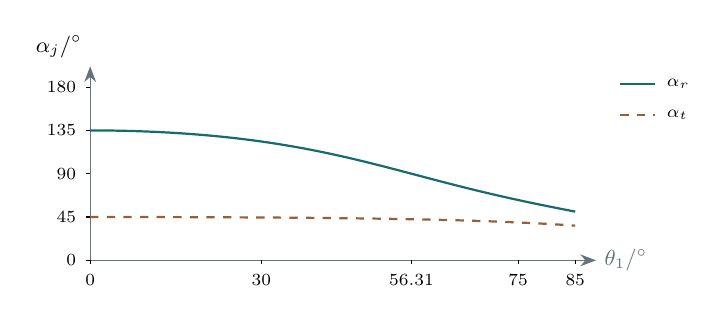
\begin{tikzpicture}[scale=.88,transform shape]
\draw[axis] (0,0.0)--(7.3,0.0) node[right] {$\theta_1/^\circ$};
\draw[axis] (0,0)--(0,2.8);
\node[above left] at (0,2.8) {$\alpha_j/^\circ$};
\draw[thin] (0.000000,0.0)--(0.000000,-0.06);\node[below,font=\scriptsize] at (0.000000,-0.08) {$ 0 $};
\draw[thin] (2.470588,0.0)--(2.470588,-0.06);\node[below,font=\scriptsize] at (2.470588,-0.08) {$ 30 $};
\draw[thin] (4.637294,0.0)--(4.637294,-0.06);\node[below,font=\scriptsize] at (4.637294,-0.08) {$ 56.31 $};
\draw[thin] (6.176471,0.0)--(6.176471,-0.06);\node[below,font=\scriptsize] at (6.176471,-0.08) {$ 75 $};
\draw[thin] (7.000000,0.0)--(7.000000,-0.06);\node[below,font=\scriptsize] at (7.000000,-0.08) {$ 85 $};
\draw[thin] (0,0.000000)--(-.06,0.000000);\node[left,font=\scriptsize] at (-.08,0.000000) {$ 0 $};
\draw[thin] (0,0.625000)--(-.06,0.625000);\node[left,font=\scriptsize] at (-.08,0.625000) {$ 45 $};
\draw[thin] (0,1.250000)--(-.06,1.250000);\node[left,font=\scriptsize] at (-.08,1.250000) {$ 90 $};
\draw[thin] (0,1.875000)--(-.06,1.875000);\node[left,font=\scriptsize] at (-.08,1.875000) {$ 135 $};
\draw[thin] (0,2.500000)--(-.06,2.500000);\node[left,font=\scriptsize] at (-.08,2.500000) {$ 180 $};
\draw[thick,color=accent] plot coordinates {(0.0000000,1.8750000) (0.0291667,1.8749797) (0.0583333,1.8749189) (0.0875000,1.8748175) (0.1166667,1.8746756) (0.1458333,1.8744930) (0.1750000,1.8742699) (0.2041667,1.8740060) (0.2333333,1.8737014) (0.2625000,1.8733561) (0.2916667,1.8729699) (0.3208333,1.8725428) (0.3500000,1.8720748) (0.3791667,1.8715657) (0.4083333,1.8710154) (0.4375000,1.8704239) (0.4666667,1.8697910) (0.4958333,1.8691166) (0.5250000,1.8684007) (0.5541667,1.8676431) (0.5833333,1.8668436) (0.6125000,1.8660021) (0.6416667,1.8651185) (0.6708333,1.8641926) (0.7000000,1.8632243) (0.7291667,1.8622134) (0.7583333,1.8611596) (0.7875000,1.8600629) (0.8166667,1.8589230) (0.8458333,1.8577398) (0.8750000,1.8565130) (0.9041667,1.8552425) (0.9333333,1.8539279) (0.9625000,1.8525692) (0.9916667,1.8511660) (1.0208333,1.8497181) (1.0500000,1.8482253) (1.0791667,1.8466873) (1.1083333,1.8451039) (1.1375000,1.8434748) (1.1666667,1.8417998) (1.1958333,1.8400785) (1.2250000,1.8383108) (1.2541667,1.8364962) (1.2833333,1.8346345) (1.3125000,1.8327254) (1.3416667,1.8307686) (1.3708333,1.8287639) (1.4000000,1.8267108) (1.4291667,1.8246090) (1.4583333,1.8224583) (1.4875000,1.8202583) (1.5166667,1.8180087) (1.5458333,1.8157090) (1.5750000,1.8133591) (1.6041667,1.8109585) (1.6333333,1.8085069) (1.6625000,1.8060038) (1.6916667,1.8034491) (1.7208333,1.8008422) (1.7500000,1.7981829) (1.7791667,1.7954708) (1.8083333,1.7927054) (1.8375000,1.7898865) (1.8666667,1.7870135) (1.8958333,1.7840863) (1.9250000,1.7811043) (1.9541667,1.7780673) (1.9833333,1.7749748) (2.0125000,1.7718264) (2.0416667,1.7686218) (2.0708333,1.7653606) (2.1000000,1.7620423) (2.1291667,1.7586668) (2.1583333,1.7552335) (2.1875000,1.7517421) (2.2166667,1.7481922) (2.2458333,1.7445835) (2.2750000,1.7409157) (2.3041667,1.7371883) (2.3333333,1.7334010) (2.3625000,1.7295534) (2.3916667,1.7256454) (2.4208333,1.7216764) (2.4500000,1.7176463) (2.4791667,1.7135546) (2.5083333,1.7094012) (2.5375000,1.7051857) (2.5666667,1.7009078) (2.5958333,1.6965673) (2.6250000,1.6921640) (2.6541667,1.6876976) (2.6833333,1.6831678) (2.7125000,1.6785746) (2.7416667,1.6739176) (2.7708333,1.6691969) (2.8000000,1.6644121) (2.8291667,1.6595632) (2.8583333,1.6546500) (2.8875000,1.6496725) (2.9166667,1.6446307) (2.9458333,1.6395245) (2.9750000,1.6343538) (3.0041667,1.6291188) (3.0333333,1.6238194) (3.0625000,1.6184557) (3.0916667,1.6130278) (3.1208333,1.6075359) (3.1500000,1.6019801) (3.1791667,1.5963607) (3.2083333,1.5906777) (3.2375000,1.5849316) (3.2666667,1.5791226) (3.2958333,1.5732511) (3.3250000,1.5673173) (3.3541667,1.5613218) (3.3833333,1.5552650) (3.4125000,1.5491474) (3.4416667,1.5429694) (3.4708333,1.5367318) (3.5000000,1.5304350) (3.5291667,1.5240798) (3.5583333,1.5176668) (3.5875000,1.5111969) (3.6166667,1.5046706) (3.6458333,1.4980890) (3.6750000,1.4914529) (3.7041667,1.4847631) (3.7333333,1.4780207) (3.7625000,1.4712267) (3.7916667,1.4643820) (3.8208333,1.4574878) (3.8500000,1.4505453) (3.8791667,1.4435555) (3.9083333,1.4365198) (3.9375000,1.4294393) (3.9666667,1.4223153) (3.9958333,1.4151493) (4.0250000,1.4079425) (4.0541667,1.4006965) (4.0833333,1.3934125) (4.1125000,1.3860921) (4.1416667,1.3787369) (4.1708333,1.3713483) (4.2000000,1.3639279) (4.2291667,1.3564774) (4.2583333,1.3489983) (4.2875000,1.3414924) (4.3166667,1.3339612) (4.3458333,1.3264064) (4.3750000,1.3188298) (4.4041667,1.3112331) (4.4333333,1.3036180) (4.4625000,1.2959862) (4.4916667,1.2883396) (4.5208333,1.2806798) (4.5500000,1.2730086) (4.5791667,1.2653277) (4.6083333,1.2576390) (4.6375000,1.2499442) (4.6666667,1.2422450) (4.6958333,1.2345431) (4.7250000,1.2268402) (4.7541667,1.2191381) (4.7833333,1.2114385) (4.8125000,1.2037429) (4.8416667,1.1960531) (4.8708333,1.1883707) (4.9000000,1.1806972) (4.9291667,1.1730342) (4.9583333,1.1653832) (4.9875000,1.1577458) (5.0166667,1.1501234) (5.0458333,1.1425174) (5.0750000,1.1349292) (5.1041667,1.1273601) (5.1333333,1.1198115) (5.1625000,1.1122847) (5.1916667,1.1047807) (5.2208333,1.0973009) (5.2500000,1.0898463) (5.2791667,1.0824180) (5.3083333,1.0750171) (5.3375000,1.0676444) (5.3666667,1.0603010) (5.3958333,1.0529878) (5.4250000,1.0457055) (5.4541667,1.0384550) (5.4833333,1.0312369) (5.5125000,1.0240520) (5.5416667,1.0169009) (5.5708333,1.0097841) (5.6000000,1.0027022) (5.6291667,0.9956556) (5.6583333,0.9886449) (5.6875000,0.9816703) (5.7166667,0.9747322) (5.7458333,0.9678308) (5.7750000,0.9609664) (5.8041667,0.9541392) (5.8333333,0.9473493) (5.8625000,0.9405968) (5.8916667,0.9338817) (5.9208333,0.9272041) (5.9500000,0.9205638) (5.9791667,0.9139609) (6.0083333,0.9073951) (6.0375000,0.9008663) (6.0666667,0.8943743) (6.0958333,0.8879189) (6.1250000,0.8814998) (6.1541667,0.8751165) (6.1833333,0.8687689) (6.2125000,0.8624565) (6.2416667,0.8561788) (6.2708333,0.8499355) (6.3000000,0.8437259) (6.3291667,0.8375497) (6.3583333,0.8314062) (6.3875000,0.8252949) (6.4166667,0.8192152) (6.4458333,0.8131664) (6.4750000,0.8071479) (6.5041667,0.8011591) (6.5333333,0.7951991) (6.5625000,0.7892673) (6.5916667,0.7833630) (6.6208333,0.7774853) (6.6500000,0.7716335) (6.6791667,0.7658067) (6.7083333,0.7600043) (6.7375000,0.7542252) (6.7666667,0.7484687) (6.7958333,0.7427339) (6.8250000,0.7370199) (6.8541667,0.7313258) (6.8833333,0.7256507) (6.9125000,0.7199936) (6.9416667,0.7143537) (6.9708333,0.7087299) (7.0000000,0.7031214)};
\draw[thick,color=accent] (7.65,2.55)--(8.15,2.55);\node[right,font=\scriptsize] at (8.2,2.55) {$\alpha_r$};
\draw[thick,dashed,color=warm] plot coordinates {(0.0000000,0.6250000) (0.0291667,0.6249992) (0.0583333,0.6249966) (0.0875000,0.6249924) (0.1166667,0.6249865) (0.1458333,0.6249789) (0.1750000,0.6249696) (0.2041667,0.6249586) (0.2333333,0.6249459) (0.2625000,0.6249315) (0.2916667,0.6249154) (0.3208333,0.6248976) (0.3500000,0.6248781) (0.3791667,0.6248569) (0.4083333,0.6248340) (0.4375000,0.6248093) (0.4666667,0.6247830) (0.4958333,0.6247549) (0.5250000,0.6247250) (0.5541667,0.6246935) (0.5833333,0.6246601) (0.6125000,0.6246251) (0.6416667,0.6245883) (0.6708333,0.6245497) (0.7000000,0.6245093) (0.7291667,0.6244672) (0.7583333,0.6244233) (0.7875000,0.6243776) (0.8166667,0.6243300) (0.8458333,0.6242807) (0.8750000,0.6242296) (0.9041667,0.6241766) (0.9333333,0.6241218) (0.9625000,0.6240652) (0.9916667,0.6240067) (1.0208333,0.6239463) (1.0500000,0.6238840) (1.0791667,0.6238199) (1.1083333,0.6237538) (1.1375000,0.6236859) (1.1666667,0.6236160) (1.1958333,0.6235441) (1.2250000,0.6234703) (1.2541667,0.6233946) (1.2833333,0.6233169) (1.3125000,0.6232371) (1.3416667,0.6231554) (1.3708333,0.6230716) (1.4000000,0.6229858) (1.4291667,0.6228979) (1.4583333,0.6228080) (1.4875000,0.6227160) (1.5166667,0.6226218) (1.5458333,0.6225256) (1.5750000,0.6224272) (1.6041667,0.6223266) (1.6333333,0.6222238) (1.6625000,0.6221189) (1.6916667,0.6220117) (1.7208333,0.6219023) (1.7500000,0.6217906) (1.7791667,0.6216767) (1.8083333,0.6215604) (1.8375000,0.6214418) (1.8666667,0.6213209) (1.8958333,0.6211976) (1.9250000,0.6210718) (1.9541667,0.6209437) (1.9833333,0.6208131) (2.0125000,0.6206801) (2.0416667,0.6205445) (2.0708333,0.6204064) (2.1000000,0.6202658) (2.1291667,0.6201226) (2.1583333,0.6199768) (2.1875000,0.6198283) (2.2166667,0.6196772) (2.2458333,0.6195234) (2.2750000,0.6193668) (2.3041667,0.6192075) (2.3333333,0.6190454) (2.3625000,0.6188805) (2.3916667,0.6187127) (2.4208333,0.6185421) (2.4500000,0.6183685) (2.4791667,0.6181919) (2.5083333,0.6180124) (2.5375000,0.6178298) (2.5666667,0.6176441) (2.5958333,0.6174554) (2.6250000,0.6172635) (2.6541667,0.6170684) (2.6833333,0.6168700) (2.7125000,0.6166684) (2.7416667,0.6164635) (2.7708333,0.6162553) (2.8000000,0.6160436) (2.8291667,0.6158285) (2.8583333,0.6156099) (2.8875000,0.6153878) (2.9166667,0.6151621) (2.9458333,0.6149327) (2.9750000,0.6146997) (3.0041667,0.6144630) (3.0333333,0.6142225) (3.0625000,0.6139781) (3.0916667,0.6137299) (3.1208333,0.6134777) (3.1500000,0.6132215) (3.1791667,0.6129613) (3.2083333,0.6126970) (3.2375000,0.6124285) (3.2666667,0.6121557) (3.2958333,0.6118787) (3.3250000,0.6115974) (3.3541667,0.6113116) (3.3833333,0.6110214) (3.4125000,0.6107267) (3.4416667,0.6104273) (3.4708333,0.6101233) (3.5000000,0.6098145) (3.5291667,0.6095009) (3.5583333,0.6091825) (3.5875000,0.6088591) (3.6166667,0.6085306) (3.6458333,0.6081971) (3.6750000,0.6078584) (3.7041667,0.6075144) (3.7333333,0.6071651) (3.7625000,0.6068104) (3.7916667,0.6064502) (3.8208333,0.6060844) (3.8500000,0.6057129) (3.8791667,0.6053357) (3.9083333,0.6049526) (3.9375000,0.6045636) (3.9666667,0.6041686) (3.9958333,0.6037675) (4.0250000,0.6033601) (4.0541667,0.6029464) (4.0833333,0.6025264) (4.1125000,0.6020998) (4.1416667,0.6016666) (4.1708333,0.6012267) (4.2000000,0.6007799) (4.2291667,0.6003263) (4.2583333,0.5998656) (4.2875000,0.5993977) (4.3166667,0.5989226) (4.3458333,0.5984401) (4.3750000,0.5979501) (4.4041667,0.5974524) (4.4333333,0.5969470) (4.4625000,0.5964338) (4.4916667,0.5959126) (4.5208333,0.5953832) (4.5500000,0.5948456) (4.5791667,0.5942996) (4.6083333,0.5937451) (4.6375000,0.5931819) (4.6666667,0.5926099) (4.6958333,0.5920289) (4.7250000,0.5914389) (4.7541667,0.5908396) (4.7833333,0.5902309) (4.8125000,0.5896127) (4.8416667,0.5889848) (4.8708333,0.5883470) (4.9000000,0.5876992) (4.9291667,0.5870412) (4.9583333,0.5863729) (4.9875000,0.5856940) (5.0166667,0.5850044) (5.0458333,0.5843040) (5.0750000,0.5835925) (5.1041667,0.5828698) (5.1333333,0.5821356) (5.1625000,0.5813899) (5.1916667,0.5806323) (5.2208333,0.5798628) (5.2500000,0.5790810) (5.2791667,0.5782869) (5.3083333,0.5774801) (5.3375000,0.5766606) (5.3666667,0.5758280) (5.3958333,0.5749822) (5.4250000,0.5741230) (5.4541667,0.5732501) (5.4833333,0.5723632) (5.5125000,0.5714623) (5.5416667,0.5705470) (5.5708333,0.5696171) (5.6000000,0.5686723) (5.6291667,0.5677125) (5.6583333,0.5667373) (5.6875000,0.5657466) (5.7166667,0.5647400) (5.7458333,0.5637173) (5.7750000,0.5626782) (5.8041667,0.5616225) (5.8333333,0.5605500) (5.8625000,0.5594602) (5.8916667,0.5583530) (5.9208333,0.5572280) (5.9500000,0.5560850) (5.9791667,0.5549236) (6.0083333,0.5537437) (6.0375000,0.5525448) (6.0666667,0.5513266) (6.0958333,0.5500889) (6.1250000,0.5488314) (6.1541667,0.5475537) (6.1833333,0.5462555) (6.2125000,0.5449364) (6.2416667,0.5435962) (6.2708333,0.5422344) (6.3000000,0.5408508) (6.3291667,0.5394450) (6.3583333,0.5380167) (6.3875000,0.5365654) (6.4166667,0.5350909) (6.4458333,0.5335927) (6.4750000,0.5320706) (6.5041667,0.5305240) (6.5333333,0.5289527) (6.5625000,0.5273562) (6.5916667,0.5257342) (6.6208333,0.5240863) (6.6500000,0.5224120) (6.6791667,0.5207109) (6.7083333,0.5189828) (6.7375000,0.5172270) (6.7666667,0.5154433) (6.7958333,0.5136311) (6.8250000,0.5117902) (6.8541667,0.5099199) (6.8833333,0.5080200) (6.9125000,0.5060899) (6.9416667,0.5041292) (6.9708333,0.5021374) (7.0000000,0.5001142)};
\draw[thick,dashed,color=warm] (7.65,2.0999999999999996)--(8.15,2.0999999999999996);\node[right,font=\scriptsize] at (8.2,2.0999999999999996) {$\alpha_t$};
\end{tikzpicture}
\figcaption{解图光4.4B\quad 空气到玻璃，输入45度；各束采用自己的局部轴}
\end{minipage}\end{center}

\textbf{布儒斯特和法向入射。}布儒斯特角满足$\theta_1+\theta_2=\pi/2$，此时$r_p=0$。若$\sin\alpha\ne0$，反射只有$s$分量，振动垂直入射面；若入射为纯$p$，反射总场为零，偏振方向无定义。图B的反射局部轴在该角度取90°，其含义由非零的$s$分量确定。

法向入射时入射面可任选；本坐标下$\boldsymbol p_i=+x$、$\boldsymbol p_r=-x$。空气到1.50玻璃的系数为$r_p=+0.2,r_s=-0.2$，恢复全局电场可得
\[
\boldsymbol E_r=-0.2E_0(\cos\alpha\,\hat{\boldsymbol x}
+\sin\alpha\,\hat{\boldsymbol y}).
\]
反射直线与入射直线相同，共同相位改变$\pi$。局部角$\alpha_r=-\alpha\pmod\pi$与全局直线相同，差别由$p$基矢反向产生。若$n_1=n_2$，则$r_s=r_p=0,t_s=t_p=1$；透射方向保持，反射方向无定义。

\textbf{全反射后的椭圆。}当$n_1>n_2$且$\theta_1>\arcsin(n_2/n_1)$，令
\[
\kappa=\sqrt{(n_1\sin\theta_1/n_2)^2-1}>0,\qquad
\cos\theta_2=i\kappa .
\]
所选虚余弦给出沿$z>0$衰减的透射场。代入振幅式后，$|r_s|=|r_p|=1$，二者相位一般不同。纯$s$或纯$p$仍线偏振；两个非零分量需按复Jones状态求振动轨迹。第二介质中的倏逝场沿界面传播并法向衰减，常规远场折射束的线轴角在此情形下无定义。

采用$e^{-i\omega t}$，反射Jones向量记为$(a,b)$，其瞬时轨迹为$(\operatorname{Re}ae^{-i\omega t},\operatorname{Re}be^{-i\omega t})$。定义
\[
S_0=|a|^2+|b|^2,\quad S_1=|a|^2-|b|^2,\quad
S_2=2\operatorname{Re}(ab^*),\quad S_3=-2\operatorname{Im}(ab^*).
\]
非圆椭圆主轴为$\psi=\tfrac12\operatorname{atan2}(S_2,S_1)$，椭圆率角为$\chi=\tfrac12\arcsin(S_3/S_0)$；$\operatorname{Im}(ab^*)=0$时退成直线。图C比较部分反射直线与全反射椭圆，两者各自按反射总强度归一，用来比较振动形状。

\begin{center}\begin{minipage}{.98\linewidth}\centering
\begin{tikzpicture}[scale=.9,transform shape]
\draw[axis] (-2.8,0)--(2.9,0) node[right] {$E_p/\sqrt{S_0}$};
\draw[axis] (0,-2.8)--(0,2.9) node[above] {$E_s/\sqrt{S_0}$};
\draw[thick,color=accent] plot coordinates {(1.3784974,-2.0856042) (1.3780250,-2.0848895) (1.3766082,-2.0827460) (1.3742480,-2.0791750) (1.3709459,-2.0741790) (1.3667042,-2.0677616) (1.3615258,-2.0599269) (1.3554144,-2.0506806) (1.3483739,-2.0400287) (1.3404094,-2.0279788) (1.3315263,-2.0145390) (1.3217305,-1.9997185) (1.3110290,-1.9835275) (1.2994289,-1.9659771) (1.2869382,-1.9470793) (1.2735655,-1.9268470) (1.2593201,-1.9052942) (1.2442115,-1.8824357) (1.2282502,-1.8582869) (1.2114471,-1.8328647) (1.1938138,-1.8061862) (1.1753623,-1.7782699) (1.1561052,-1.7491349) (1.1360558,-1.7188010) (1.1152278,-1.6872892) (1.0936355,-1.6546211) (1.0712937,-1.6208189) (1.0482177,-1.5859059) (1.0244232,-1.5499060) (0.9999267,-1.5128438) (0.9747449,-1.4747449) (0.9488950,-1.4356352) (0.9223948,-1.3955416) (0.8952625,-1.3544916) (0.8675165,-1.3125132) (0.8391761,-1.2696354) (0.8102605,-1.2258874) (0.7807895,-1.1812992) (0.7507835,-1.1359015) (0.7202629,-1.0897252) (0.6892487,-1.0428021) (0.6577621,-0.9951643) (0.6258247,-0.9468445) (0.5934584,-0.8978758) (0.5606854,-0.8482917) (0.5275281,-0.7981262) (0.4940093,-0.7474137) (0.4601519,-0.6961890) (0.4259791,-0.6444871) (0.3915144,-0.5923436) (0.3567814,-0.5397941) (0.3218038,-0.4868746) (0.2866057,-0.4336215) (0.2512112,-0.3800712) (0.2156445,-0.3262604) (0.1799300,-0.2722260) (0.1440922,-0.2180050) (0.1081557,-0.1636346) (0.0721450,-0.1091521) (0.0360849,-0.0545948) (0.0000000,-0.0000000) (-0.0360849,0.0545948) (-0.0721450,0.1091521) (-0.1081557,0.1636346) (-0.1440922,0.2180050) (-0.1799300,0.2722260) (-0.2156445,0.3262604) (-0.2512112,0.3800712) (-0.2866057,0.4336215) (-0.3218038,0.4868746) (-0.3567814,0.5397941) (-0.3915144,0.5923436) (-0.4259791,0.6444871) (-0.4601519,0.6961890) (-0.4940093,0.7474137) (-0.5275281,0.7981262) (-0.5606854,0.8482917) (-0.5934584,0.8978758) (-0.6258247,0.9468445) (-0.6577621,0.9951643) (-0.6892487,1.0428021) (-0.7202629,1.0897252) (-0.7507835,1.1359015) (-0.7807895,1.1812992) (-0.8102605,1.2258874) (-0.8391761,1.2696354) (-0.8675165,1.3125132) (-0.8952625,1.3544916) (-0.9223948,1.3955416) (-0.9488950,1.4356352) (-0.9747449,1.4747449) (-0.9999267,1.5128438) (-1.0244232,1.5499060) (-1.0482177,1.5859059) (-1.0712937,1.6208189) (-1.0936355,1.6546211) (-1.1152278,1.6872892) (-1.1360558,1.7188010) (-1.1561052,1.7491349) (-1.1753623,1.7782699) (-1.1938138,1.8061862) (-1.2114471,1.8328647) (-1.2282502,1.8582869) (-1.2442115,1.8824357) (-1.2593201,1.9052942) (-1.2735655,1.9268470) (-1.2869382,1.9470793) (-1.2994289,1.9659771) (-1.3110290,1.9835275) (-1.3217305,1.9997185) (-1.3315263,2.0145390) (-1.3404094,2.0279788) (-1.3483739,2.0400287) (-1.3554144,2.0506806) (-1.3615258,2.0599269) (-1.3667042,2.0677616) (-1.3709459,2.0741790) (-1.3742480,2.0791750) (-1.3766082,2.0827460) (-1.3780250,2.0848895) (-1.3784974,2.0856042) (-1.3780250,2.0848895) (-1.3766082,2.0827460) (-1.3742480,2.0791750) (-1.3709459,2.0741790) (-1.3667042,2.0677616) (-1.3615258,2.0599269) (-1.3554144,2.0506806) (-1.3483739,2.0400287) (-1.3404094,2.0279788) (-1.3315263,2.0145390) (-1.3217305,1.9997185) (-1.3110290,1.9835275) (-1.2994289,1.9659771) (-1.2869382,1.9470793) (-1.2735655,1.9268470) (-1.2593201,1.9052942) (-1.2442115,1.8824357) (-1.2282502,1.8582869) (-1.2114471,1.8328647) (-1.1938138,1.8061862) (-1.1753623,1.7782699) (-1.1561052,1.7491349) (-1.1360558,1.7188010) (-1.1152278,1.6872892) (-1.0936355,1.6546211) (-1.0712937,1.6208189) (-1.0482177,1.5859059) (-1.0244232,1.5499060) (-0.9999267,1.5128438) (-0.9747449,1.4747449) (-0.9488950,1.4356352) (-0.9223948,1.3955416) (-0.8952625,1.3544916) (-0.8675165,1.3125132) (-0.8391761,1.2696354) (-0.8102605,1.2258874) (-0.7807895,1.1812992) (-0.7507835,1.1359015) (-0.7202629,1.0897252) (-0.6892487,1.0428021) (-0.6577621,0.9951643) (-0.6258247,0.9468445) (-0.5934584,0.8978758) (-0.5606854,0.8482917) (-0.5275281,0.7981262) (-0.4940093,0.7474137) (-0.4601519,0.6961890) (-0.4259791,0.6444871) (-0.3915144,0.5923436) (-0.3567814,0.5397941) (-0.3218038,0.4868746) (-0.2866057,0.4336215) (-0.2512112,0.3800712) (-0.2156445,0.3262604) (-0.1799300,0.2722260) (-0.1440922,0.2180050) (-0.1081557,0.1636346) (-0.0721450,0.1091521) (-0.0360849,0.0545948) (-0.0000000,0.0000000) (0.0360849,-0.0545948) (0.0721450,-0.1091521) (0.1081557,-0.1636346) (0.1440922,-0.2180050) (0.1799300,-0.2722260) (0.2156445,-0.3262604) (0.2512112,-0.3800712) (0.2866057,-0.4336215) (0.3218038,-0.4868746) (0.3567814,-0.5397941) (0.3915144,-0.5923436) (0.4259791,-0.6444871) (0.4601519,-0.6961890) (0.4940093,-0.7474137) (0.5275281,-0.7981262) (0.5606854,-0.8482917) (0.5934584,-0.8978758) (0.6258247,-0.9468445) (0.6577621,-0.9951643) (0.6892487,-1.0428021) (0.7202629,-1.0897252) (0.7507835,-1.1359015) (0.7807895,-1.1812992) (0.8102605,-1.2258874) (0.8391761,-1.2696354) (0.8675165,-1.3125132) (0.8952625,-1.3544916) (0.9223948,-1.3955416) (0.9488950,-1.4356352) (0.9747449,-1.4747449) (0.9999267,-1.5128438) (1.0244232,-1.5499060) (1.0482177,-1.5859059) (1.0712937,-1.6208189) (1.0936355,-1.6546211) (1.1152278,-1.6872892) (1.1360558,-1.7188010) (1.1561052,-1.7491349) (1.1753623,-1.7782699) (1.1938138,-1.8061862) (1.2114471,-1.8328647) (1.2282502,-1.8582869) (1.2442115,-1.8824357) (1.2593201,-1.9052942) (1.2735655,-1.9268470) (1.2869382,-1.9470793) (1.2994289,-1.9659771) (1.3110290,-1.9835275) (1.3217305,-1.9997185) (1.3315263,-2.0145390) (1.3404094,-2.0279788) (1.3483739,-2.0400287) (1.3554144,-2.0506806) (1.3615258,-2.0599269) (1.3667042,-2.0677616) (1.3709459,-2.0741790) (1.3742480,-2.0791750) (1.3766082,-2.0827460) (1.3780250,-2.0848895) (1.3784974,-2.0856042)};
\draw[thick,color=accent] (3.3,2.45)--(3.8,2.45);\node[right,font=\scriptsize] at (3.85,2.45) {$\mathrm{partial}$};
\draw[thick,dashed,color=warm] plot coordinates {(0.4949747,1.4142136) (0.4503814,1.3859641) (0.4054793,1.3567648) (0.3602994,1.3266356) (0.3148725,1.2955972) (0.2692299,1.2636708) (0.2234027,1.2308784) (0.1774224,1.1972425) (0.1313205,1.1627860) (0.0851286,1.1275325) (0.0388784,1.0915064) (-0.0073985,1.0547321) (-0.0536703,1.0172350) (-0.0999053,0.9790407) (-0.1460718,0.9401755) (-0.1921383,0.9006659) (-0.2380730,0.8605390) (-0.2838446,0.8198224) (-0.3294217,0.7785439) (-0.3747730,0.7367318) (-0.4198674,0.6944148) (-0.4646741,0.6516219) (-0.5091623,0.6083824) (-0.5533016,0.5647259) (-0.5970617,0.5206824) (-0.6404125,0.4762821) (-0.6833245,0.4315553) (-0.7257681,0.3865328) (-0.7677144,0.3412453) (-0.8091345,0.2957240) (-0.8500000,0.2500000) (-0.8902830,0.2041047) (-0.9299558,0.1580695) (-0.9689913,0.1119259) (-1.0073627,0.0657057) (-1.0450437,0.0194404) (-1.0820085,-0.0268382) (-1.1182317,-0.0730984) (-1.1536886,-0.1193086) (-1.1883547,-0.1654369) (-1.2222065,-0.2114519) (-1.2552206,-0.2573219) (-1.2873744,-0.3030156) (-1.3186459,-0.3485016) (-1.3490137,-0.3937488) (-1.3784569,-0.4387261) (-1.4069554,-0.4834028) (-1.4344897,-0.5277481) (-1.4610408,-0.5717317) (-1.4865906,-0.6153236) (-1.5111216,-0.6584936) (-1.5346169,-0.7012124) (-1.5570605,-0.7434507) (-1.5784369,-0.7851794) (-1.5987316,-0.8263699) (-1.6179306,-0.8669942) (-1.6360207,-0.9070242) (-1.6529895,-0.9464326) (-1.6688255,-0.9851924) (-1.6835178,-1.0232769) (-1.6970563,-1.0606602) (-1.7094317,-1.0973165) (-1.7206355,-1.1332208) (-1.7306601,-1.1683484) (-1.7394986,-1.2026753) (-1.7471449,-1.2361780) (-1.7535938,-1.2688334) (-1.7588409,-1.3006193) (-1.7628826,-1.3315137) (-1.7657160,-1.3614956) (-1.7673394,-1.3905445) (-1.7677515,-1.4186403) (-1.7669520,-1.4457638) (-1.7649416,-1.4718965) (-1.7617216,-1.4970204) (-1.7572942,-1.5211183) (-1.7516624,-1.5441738) (-1.7448301,-1.5661709) (-1.7368020,-1.5870947) (-1.7275836,-1.6069307) (-1.7171812,-1.6256654) (-1.7056019,-1.6432860) (-1.6928537,-1.6597804) (-1.6789453,-1.6751372) (-1.6638862,-1.6893460) (-1.6476868,-1.7023970) (-1.6303581,-1.7142812) (-1.6119121,-1.7249906) (-1.5923613,-1.7345177) (-1.5717193,-1.7428561) (-1.5500000,-1.7500000) (-1.5272184,-1.7559446) (-1.5033902,-1.7606857) (-1.4785316,-1.7642201) (-1.4526597,-1.7665454) (-1.4257923,-1.7676601) (-1.3979476,-1.7675632) (-1.3691449,-1.7662550) (-1.3394038,-1.7637362) (-1.3087448,-1.7600087) (-1.2771888,-1.7550750) (-1.2447575,-1.7489384) (-1.2114732,-1.7416032) (-1.1773585,-1.7330743) (-1.1424369,-1.7233577) (-1.1067324,-1.7124600) (-1.0702693,-1.7003887) (-1.0330728,-1.6871520) (-0.9951682,-1.6727590) (-0.9565816,-1.6572196) (-0.9173394,-1.6405445) (-0.8774685,-1.6227449) (-0.8369962,-1.6038333) (-0.7959503,-1.5838224) (-0.7543589,-1.5627261) (-0.7122505,-1.5405587) (-0.6696539,-1.5173355) (-0.6265984,-1.4930725) (-0.5831135,-1.4677861) (-0.5392289,-1.4414938) (-0.4949747,-1.4142136) (-0.4503814,-1.3859641) (-0.4054793,-1.3567648) (-0.3602994,-1.3266356) (-0.3148725,-1.2955972) (-0.2692299,-1.2636708) (-0.2234027,-1.2308784) (-0.1774224,-1.1972425) (-0.1313205,-1.1627860) (-0.0851286,-1.1275325) (-0.0388784,-1.0915064) (0.0073985,-1.0547321) (0.0536703,-1.0172350) (0.0999053,-0.9790407) (0.1460718,-0.9401755) (0.1921383,-0.9006659) (0.2380730,-0.8605390) (0.2838446,-0.8198224) (0.3294217,-0.7785439) (0.3747730,-0.7367318) (0.4198674,-0.6944148) (0.4646741,-0.6516219) (0.5091623,-0.6083824) (0.5533016,-0.5647259) (0.5970617,-0.5206824) (0.6404125,-0.4762821) (0.6833245,-0.4315553) (0.7257681,-0.3865328) (0.7677144,-0.3412453) (0.8091345,-0.2957240) (0.8500000,-0.2500000) (0.8902830,-0.2041047) (0.9299558,-0.1580695) (0.9689913,-0.1119259) (1.0073627,-0.0657057) (1.0450437,-0.0194404) (1.0820085,0.0268382) (1.1182317,0.0730984) (1.1536886,0.1193086) (1.1883547,0.1654369) (1.2222065,0.2114519) (1.2552206,0.2573219) (1.2873744,0.3030156) (1.3186459,0.3485016) (1.3490137,0.3937488) (1.3784569,0.4387261) (1.4069554,0.4834028) (1.4344897,0.5277481) (1.4610408,0.5717317) (1.4865906,0.6153236) (1.5111216,0.6584936) (1.5346169,0.7012124) (1.5570605,0.7434507) (1.5784369,0.7851794) (1.5987316,0.8263699) (1.6179306,0.8669942) (1.6360207,0.9070242) (1.6529895,0.9464326) (1.6688255,0.9851924) (1.6835178,1.0232769) (1.6970563,1.0606602) (1.7094317,1.0973165) (1.7206355,1.1332208) (1.7306601,1.1683484) (1.7394986,1.2026753) (1.7471449,1.2361780) (1.7535938,1.2688334) (1.7588409,1.3006193) (1.7628826,1.3315137) (1.7657160,1.3614956) (1.7673394,1.3905445) (1.7677515,1.4186403) (1.7669520,1.4457638) (1.7649416,1.4718965) (1.7617216,1.4970204) (1.7572942,1.5211183) (1.7516624,1.5441738) (1.7448301,1.5661709) (1.7368020,1.5870947) (1.7275836,1.6069307) (1.7171812,1.6256654) (1.7056019,1.6432860) (1.6928537,1.6597804) (1.6789453,1.6751372) (1.6638862,1.6893460) (1.6476868,1.7023970) (1.6303581,1.7142812) (1.6119121,1.7249906) (1.5923613,1.7345177) (1.5717193,1.7428561) (1.5500000,1.7500000) (1.5272184,1.7559446) (1.5033902,1.7606857) (1.4785316,1.7642201) (1.4526597,1.7665454) (1.4257923,1.7676601) (1.3979476,1.7675632) (1.3691449,1.7662550) (1.3394038,1.7637362) (1.3087448,1.7600087) (1.2771888,1.7550750) (1.2447575,1.7489384) (1.2114732,1.7416032) (1.1773585,1.7330743) (1.1424369,1.7233577) (1.1067324,1.7124600) (1.0702693,1.7003887) (1.0330728,1.6871520) (0.9951682,1.6727590) (0.9565816,1.6572196) (0.9173394,1.6405445) (0.8774685,1.6227449) (0.8369962,1.6038333) (0.7959503,1.5838224) (0.7543589,1.5627261) (0.7122505,1.5405587) (0.6696539,1.5173355) (0.6265984,1.4930725) (0.5831135,1.4677861) (0.5392289,1.4414938) (0.4949747,1.4142136)};
\draw[thick,dashed,color=warm] (3.3,1.9500000000000002)--(3.8,1.9500000000000002);\node[right,font=\scriptsize] at (3.85,1.9500000000000002) {$\mathrm{TIR}$};
\end{tikzpicture}
\figcaption{解图光4.4C\quad 线偏振部分反射的直线与全反射椭圆，各自归一}
\end{minipage}\end{center}

图D取$n_1/n_2=1.50$，给出相对相位$\delta=\arg(r_s/r_p)$随内部入射角的变化。图C的振动椭圆由两分量的幅度与相对相位共同确定；图D单独显示这项相对延迟。

\begin{center}\begin{minipage}{.98\linewidth}\centering
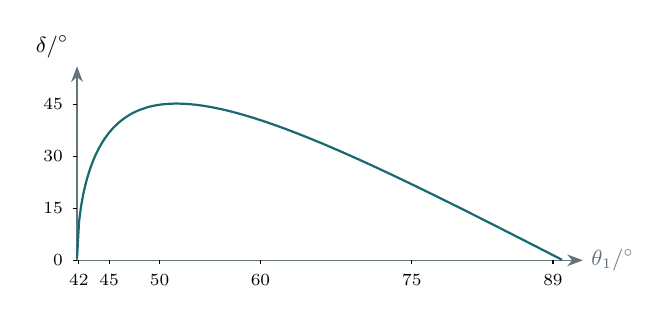
\begin{tikzpicture}[scale=.88,transform shape]
\draw[axis] (0,0.0)--(7.3,0.0) node[right] {$\theta_1/^\circ$};
\draw[axis] (0,0)--(0,2.8);
\node[above left] at (0,2.8) {$\delta/^\circ$};
\draw[thin] (0.027511,0.0)--(0.027511,-0.06);\node[below,font=\scriptsize] at (0.027511,-0.08) {$ 42 $};
\draw[thin] (0.464202,0.0)--(0.464202,-0.06);\node[below,font=\scriptsize] at (0.464202,-0.08) {$ 45 $};
\draw[thin] (1.192019,0.0)--(1.192019,-0.06);\node[below,font=\scriptsize] at (1.192019,-0.08) {$ 50 $};
\draw[thin] (2.647653,0.0)--(2.647653,-0.06);\node[below,font=\scriptsize] at (2.647653,-0.08) {$ 60 $};
\draw[thin] (4.831105,0.0)--(4.831105,-0.06);\node[below,font=\scriptsize] at (4.831105,-0.08) {$ 75 $};
\draw[thin] (6.868993,0.0)--(6.868993,-0.06);\node[below,font=\scriptsize] at (6.868993,-0.08) {$ 89 $};
\draw[thin] (0,0.000000)--(-.06,0.000000);\node[left,font=\scriptsize] at (-.08,0.000000) {$ 0 $};
\draw[thin] (0,0.750000)--(-.06,0.750000);\node[left,font=\scriptsize] at (-.08,0.750000) {$ 15 $};
\draw[thin] (0,1.500000)--(-.06,1.500000);\node[left,font=\scriptsize] at (-.08,1.500000) {$ 30 $};
\draw[thin] (0,2.250000)--(-.06,2.250000);\node[left,font=\scriptsize] at (-.08,2.250000) {$ 45 $};
\draw[thick,color=accent] plot coordinates {(0.0000000,0.0331220) (0.0291667,0.5595684) (0.0583333,0.7798915) (0.0875000,0.9420378) (0.1166667,1.0731495) (0.1458333,1.1839446) (0.1750000,1.2800187) (0.2041667,1.3647526) (0.2333333,1.4403850) (0.2625000,1.5084951) (0.2916667,1.5702496) (0.3208333,1.6265417) (0.3500000,1.6780741) (0.3791667,1.7254126) (0.4083333,1.7690211) (0.4375000,1.8092859) (0.4666667,1.8465331) (0.4958333,1.8810409) (0.5250000,1.9130492) (0.5541667,1.9427664) (0.5833333,1.9703752) (0.6125000,1.9960366) (0.6416667,2.0198936) (0.6708333,2.0420735) (0.7000000,2.0626907) (0.7291667,2.0818479) (0.7583333,2.0996382) (0.7875000,2.1161460) (0.8166667,2.1314481) (0.8458333,2.1456148) (0.8750000,2.1587103) (0.9041667,2.1707937) (0.9333333,2.1819194) (0.9625000,2.1921376) (0.9916667,2.2014949) (1.0208333,2.2100342) (1.0500000,2.2177957) (1.0791667,2.2248165) (1.1083333,2.2311314) (1.1375000,2.2367728) (1.1666667,2.2417710) (1.1958333,2.2461544) (1.2250000,2.2499497) (1.2541667,2.2531819) (1.2833333,2.2558745) (1.3125000,2.2580498) (1.3416667,2.2597285) (1.3708333,2.2609304) (1.4000000,2.2616741) (1.4291667,2.2619772) (1.4583333,2.2618565) (1.4875000,2.2613277) (1.5166667,2.2604057) (1.5458333,2.2591049) (1.5750000,2.2574388) (1.6041667,2.2554201) (1.6333333,2.2530612) (1.6625000,2.2503736) (1.6916667,2.2473684) (1.7208333,2.2440564) (1.7500000,2.2404474) (1.7791667,2.2365513) (1.8083333,2.2323772) (1.8375000,2.2279338) (1.8666667,2.2232298) (1.8958333,2.2182731) (1.9250000,2.2130714) (1.9541667,2.2076323) (1.9833333,2.2019627) (2.0125000,2.1960695) (2.0416667,2.1899593) (2.0708333,2.1836383) (2.1000000,2.1771126) (2.1291667,2.1703880) (2.1583333,2.1634701) (2.1875000,2.1563642) (2.2166667,2.1490756) (2.2458333,2.1416092) (2.2750000,2.1339698) (2.3041667,2.1261620) (2.3333333,2.1181904) (2.3625000,2.1100591) (2.3916667,2.1017725) (2.4208333,2.0933344) (2.4500000,2.0847488) (2.4791667,2.0760194) (2.5083333,2.0671498) (2.5375000,2.0581435) (2.5666667,2.0490039) (2.5958333,2.0397343) (2.6250000,2.0303378) (2.6541667,2.0208176) (2.6833333,2.0111765) (2.7125000,2.0014174) (2.7416667,1.9915432) (2.7708333,1.9815566) (2.8000000,1.9714601) (2.8291667,1.9612563) (2.8583333,1.9509476) (2.8875000,1.9405366) (2.9166667,1.9300254) (2.9458333,1.9194163) (2.9750000,1.9087116) (3.0041667,1.8979133) (3.0333333,1.8870235) (3.0625000,1.8760443) (3.0916667,1.8649775) (3.1208333,1.8538251) (3.1500000,1.8425889) (3.1791667,1.8312708) (3.2083333,1.8198724) (3.2375000,1.8083955) (3.2666667,1.7968417) (3.2958333,1.7852127) (3.3250000,1.7735100) (3.3541667,1.7617352) (3.3833333,1.7498897) (3.4125000,1.7379750) (3.4416667,1.7259925) (3.4708333,1.7139436) (3.5000000,1.7018297) (3.5291667,1.6896521) (3.5583333,1.6774120) (3.5875000,1.6651107) (3.6166667,1.6527494) (3.6458333,1.6403294) (3.6750000,1.6278518) (3.7041667,1.6153177) (3.7333333,1.6027283) (3.7625000,1.5900846) (3.7916667,1.5773878) (3.8208333,1.5646387) (3.8500000,1.5518386) (3.8791667,1.5389883) (3.9083333,1.5260888) (3.9375000,1.5131411) (3.9666667,1.5001461) (3.9958333,1.4871047) (4.0250000,1.4740179) (4.0541667,1.4608865) (4.0833333,1.4477113) (4.1125000,1.4344931) (4.1416667,1.4212329) (4.1708333,1.4079314) (4.2000000,1.3945894) (4.2291667,1.3812077) (4.2583333,1.3677870) (4.2875000,1.3543281) (4.3166667,1.3408317) (4.3458333,1.3272984) (4.3750000,1.3137291) (4.4041667,1.3001244) (4.4333333,1.2864850) (4.4625000,1.2728115) (4.4916667,1.2591046) (4.5208333,1.2453649) (4.5500000,1.2315931) (4.5791667,1.2177897) (4.6083333,1.2039555) (4.6375000,1.1900909) (4.6666667,1.1761965) (4.6958333,1.1622730) (4.7250000,1.1483208) (4.7541667,1.1343406) (4.7833333,1.1203329) (4.8125000,1.1062982) (4.8416667,1.0922371) (4.8708333,1.0781501) (4.9000000,1.0640376) (4.9291667,1.0499002) (4.9583333,1.0357385) (4.9875000,1.0215528) (5.0166667,1.0073436) (5.0458333,0.9931115) (5.0750000,0.9788569) (5.1041667,0.9645802) (5.1333333,0.9502820) (5.1625000,0.9359626) (5.1916667,0.9216225) (5.2208333,0.9072622) (5.2500000,0.8928820) (5.2791667,0.8784824) (5.3083333,0.8640638) (5.3375000,0.8496266) (5.3666667,0.8351713) (5.3958333,0.8206981) (5.4250000,0.8062076) (5.4541667,0.7917001) (5.4833333,0.7771760) (5.5125000,0.7626357) (5.5416667,0.7480795) (5.5708333,0.7335079) (5.6000000,0.7189212) (5.6291667,0.7043197) (5.6583333,0.6897038) (5.6875000,0.6750740) (5.7166667,0.6604305) (5.7458333,0.6457736) (5.7750000,0.6311038) (5.8041667,0.6164214) (5.8333333,0.6017267) (5.8625000,0.5870200) (5.8916667,0.5723018) (5.9208333,0.5575722) (5.9500000,0.5428317) (5.9791667,0.5280806) (6.0083333,0.5133191) (6.0375000,0.4985477) (6.0666667,0.4837665) (6.0958333,0.4689761) (6.1250000,0.4541765) (6.1541667,0.4393683) (6.1833333,0.4245515) (6.2125000,0.4097267) (6.2416667,0.3948941) (6.2708333,0.3800539) (6.3000000,0.3652065) (6.3291667,0.3503521) (6.3583333,0.3354912) (6.3875000,0.3206238) (6.4166667,0.3057505) (6.4458333,0.2908714) (6.4750000,0.2759868) (6.5041667,0.2610971) (6.5333333,0.2462024) (6.5625000,0.2313032) (6.5916667,0.2163996) (6.6208333,0.2014920) (6.6500000,0.1865807) (6.6791667,0.1716659) (6.7083333,0.1567479) (6.7375000,0.1418269) (6.7666667,0.1269034) (6.7958333,0.1119775) (6.8250000,0.0970495) (6.8541667,0.0821197) (6.8833333,0.0671884) (6.9125000,0.0522559) (6.9416667,0.0373224) (6.9708333,0.0223882) (7.0000000,0.0074536)};
\end{tikzpicture}
\figcaption{解图光4.4D\quad 玻璃到空气全反射的两偏振相对延迟}
\end{minipage}\end{center}

吸收介质应使用复折射率，并选向介质内部衰减的法向波数分支。反射束仍在透明介质中，可由上述复Jones向量求椭圆；吸收介质内的透射场需保留其完整复波矢和电场。


\Needspace{13\baselineskip}

\pdfbookmark[2]{第 5 题 斜反射自然光的偏振度}{q5}

\section*{第 5 题\quad 斜反射自然光的偏振度}\label{q:5}

自然光从空气以$30^\circ$入射角照射折射率为1.50的玻璃平面。求反射光的线偏振度及较强分量的方向。玻璃透明、非磁性。

\begin{center}\begin{minipage}{.98\linewidth}\centering
\begin{tikzpicture}[scale=.9,transform shape]
\draw[object] (-3.10000,0.00000)--(3.50000,0.00000);\draw[guide] (0.00000,-2.50000)--(0.00000,2.70000);\fill (0.00000,0.00000) circle(.035);\node[above right] at (0.00000,0.00000) {$O$};\draw[motion] (-1.25000,2.16506)--(0.00000,0.00000);
\draw[motion] (0.00000,0.00000)--(1.25000,2.16506);\draw[motion] (0.00000,0.00000)--(0.83333,-2.35702);\node[right] at (-2.90000,1.50000) {$n_1$};\node[right] at (-2.90000,-1.50000) {$n_2$};\node[left] at (-0.50000,1.00000) {$\theta_i$};\node[right] at (0.55000,1.10000) {$\theta_r$};\node[right] at (0.42000,-1.00000) {$\theta_t$};\node[right] at (2.50000,-2.30000) {$n_2=1.50$};
\end{tikzpicture}
\figcaption{图光4.5\quad 自然光以30度入射玻璃}
\end{minipage}\end{center}

\Needspace{6\baselineskip}\subsection*{解答}


\textbf{先分配入射强度，再求界面振幅。}取$p$在入射面内、$s$垂直入射面，强度$I_0$为入射自然光总强度。把自然光分为各含$I_0/2$的两正交且不相干分量。折射角先由Snell定律求出：
\[
\sin\theta_t=\frac{\sin30^\circ}{1.50}=\frac13,
\qquad\theta_t=19.4712^\circ
\]
将此角代入局部有向Fresnel振幅式，得
\[
r_s=\frac{\cos30^\circ-1.5\cos\theta_t}{\cos30^\circ+1.5\cos\theta_t}
=-0.240408,
\quad
r_p=\frac{1.5\cos30^\circ-\cos\theta_t}{1.5\cos30^\circ+\cos\theta_t}
=0.158900.
\]
反射与入射均在空气中，强度反射率直接取相应振幅模平方：
\[
R_s=|r_s|^2=0.0577961,\quad R_p=|r_p|^2=0.0252491,
\]
因此反射束的两个正交强度为
\[
I_s=0.0288981I_0,\qquad I_p=0.0126246I_0.
\]
图A把它们按同一$I_0$列出，虚线高度是两分量中较小的$I_p$。

\begin{center}\begin{minipage}{.98\linewidth}\centering
\begin{tikzpicture}[scale=.9,transform shape]
\draw[axis] (0.00000,0.00000)--(5.00000,0.00000);\node[right] at (5.00000,0.00000) {分量};\draw[very thick,color=accent] (1.00000,0.00000)--(1.00000,2.2890320);\node[above] at (1.00000,2.2890320) {$I_s=0.028898I_0$};\draw[very thick,color=accent] (3.50000,0.00000)--(3.50000,1.00000);\node[above] at (3.50000,1.00000) {$I_p=0.012625I_0$};\draw[guide] (0.20000,1.00000)--(4.30000,1.00000);\node[below] at (2.50000,-0.60000) {共同部分组成自然背景};
\end{tikzpicture}
\figcaption{解图光4.5A\quad 反射分量的强度差与总强度}
\end{minipage}\end{center}

\textbf{由实际检偏读数求偏振度。}设理想检偏轴与$s$夹角为$\beta$，两个不相干分量投影后的强度相加：
\[
I_{\rm an}(\beta)=I_s\cos^2\beta+I_p\sin^2\beta .
\]
由于$I_s>I_p$，沿$s$时读数最大为$I_s$，沿$p$时最小为$I_p$。反射总强度为$I_R=I_s+I_p=0.0415226I_0$，故
\[
\boxed{P_L=\frac{I_s-I_p}{I_s+I_p}
=\frac{R_s-R_p}{R_s+R_p}=0.391918\simeq39.2\%}.
\]
较强分量垂直入射面。图B比较$R_s,R_p$随入射角的变化，图C给出本题30°处的实际检偏曲线；后者的两个极值正是偏振度差商的分子、分母所用读数。

\begin{center}\begin{minipage}{.98\linewidth}\centering
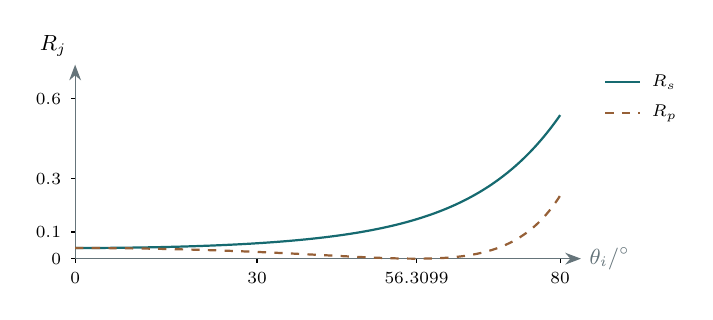
\begin{tikzpicture}[scale=.88,transform shape]
\draw[axis] (0,0.0)--(7.3,0.0) node[right] {$\theta_i/^\circ$};
\draw[axis] (0,0)--(0,2.8);
\node[above left] at (0,2.8) {$R_j$};
\draw[thin] (0.000000,0.0)--(0.000000,-0.06);\node[below,font=\scriptsize] at (0.000000,-0.08) {$ 0 $};
\draw[thin] (2.625000,0.0)--(2.625000,-0.06);\node[below,font=\scriptsize] at (2.625000,-0.08) {$ 30 $};
\draw[thin] (4.927116,0.0)--(4.927116,-0.06);\node[below,font=\scriptsize] at (4.927116,-0.08) {$ 56.3099 $};
\draw[thin] (7.000000,0.0)--(7.000000,-0.06);\node[below,font=\scriptsize] at (7.000000,-0.08) {$ 80 $};
\draw[thin] (0,0.000000)--(-.06,0.000000);\node[left,font=\scriptsize] at (-.08,0.000000) {$ 0 $};
\draw[thin] (0,0.384615)--(-.06,0.384615);\node[left,font=\scriptsize] at (-.08,0.384615) {$ 0.1 $};
\draw[thin] (0,1.153846)--(-.06,1.153846);\node[left,font=\scriptsize] at (-.08,1.153846) {$ 0.3 $};
\draw[thin] (0,2.307692)--(-.06,2.307692);\node[left,font=\scriptsize] at (-.08,2.307692) {$ 0.6 $};
\draw[thick,color=accent] plot coordinates {(0.0000000,0.1538462) (0.0291667,0.1538531) (0.0583333,0.1538739) (0.0875000,0.1539087) (0.1166667,0.1539573) (0.1458333,0.1540198) (0.1750000,0.1540963) (0.2041667,0.1541867) (0.2333333,0.1542912) (0.2625000,0.1544096) (0.2916667,0.1545421) (0.3208333,0.1546886) (0.3500000,0.1548493) (0.3791667,0.1550242) (0.4083333,0.1552132) (0.4375000,0.1554166) (0.4666667,0.1556343) (0.4958333,0.1558663) (0.5250000,0.1561129) (0.5541667,0.1563739) (0.5833333,0.1566496) (0.6125000,0.1569399) (0.6416667,0.1572450) (0.6708333,0.1575650) (0.7000000,0.1578999) (0.7291667,0.1582498) (0.7583333,0.1586149) (0.7875000,0.1589952) (0.8166667,0.1593909) (0.8458333,0.1598021) (0.8750000,0.1602288) (0.9041667,0.1606712) (0.9333333,0.1611295) (0.9625000,0.1616038) (0.9916667,0.1620942) (1.0208333,0.1626008) (1.0500000,0.1631239) (1.0791667,0.1636635) (1.1083333,0.1642198) (1.1375000,0.1647930) (1.1666667,0.1653832) (1.1958333,0.1659907) (1.2250000,0.1666155) (1.2541667,0.1672580) (1.2833333,0.1679183) (1.3125000,0.1685965) (1.3416667,0.1692929) (1.3708333,0.1700077) (1.4000000,0.1707411) (1.4291667,0.1714933) (1.4583333,0.1722646) (1.4875000,0.1730552) (1.5166667,0.1738653) (1.5458333,0.1746952) (1.5750000,0.1755451) (1.6041667,0.1764153) (1.6333333,0.1773061) (1.6625000,0.1782177) (1.6916667,0.1791505) (1.7208333,0.1801046) (1.7500000,0.1810805) (1.7791667,0.1820784) (1.8083333,0.1830986) (1.8375000,0.1841415) (1.8666667,0.1852074) (1.8958333,0.1862965) (1.9250000,0.1874094) (1.9541667,0.1885463) (1.9833333,0.1897075) (2.0125000,0.1908935) (2.0416667,0.1921047) (2.0708333,0.1933414) (2.1000000,0.1946041) (2.1291667,0.1958931) (2.1583333,0.1972089) (2.1875000,0.1985520) (2.2166667,0.1999226) (2.2458333,0.2013214) (2.2750000,0.2027488) (2.3041667,0.2042052) (2.3333333,0.2056912) (2.3625000,0.2072072) (2.3916667,0.2087538) (2.4208333,0.2103315) (2.4500000,0.2119408) (2.4791667,0.2135823) (2.5083333,0.2152565) (2.5375000,0.2169641) (2.5666667,0.2187056) (2.5958333,0.2204816) (2.6250000,0.2222927) (2.6541667,0.2241396) (2.6833333,0.2260230) (2.7125000,0.2279435) (2.7416667,0.2299017) (2.7708333,0.2318984) (2.8000000,0.2339344) (2.8291667,0.2360102) (2.8583333,0.2381268) (2.8875000,0.2402848) (2.9166667,0.2424851) (2.9458333,0.2447284) (2.9750000,0.2470156) (3.0041667,0.2493475) (3.0333333,0.2517251) (3.0625000,0.2541491) (3.0916667,0.2566205) (3.1208333,0.2591402) (3.1500000,0.2617092) (3.1791667,0.2643284) (3.2083333,0.2669989) (3.2375000,0.2697217) (3.2666667,0.2724978) (3.2958333,0.2753283) (3.3250000,0.2782142) (3.3541667,0.2811569) (3.3833333,0.2841572) (3.4125000,0.2872166) (3.4416667,0.2903361) (3.4708333,0.2935170) (3.5000000,0.2967605) (3.5291667,0.3000681) (3.5583333,0.3034409) (3.5875000,0.3068804) (3.6166667,0.3103880) (3.6458333,0.3139650) (3.6750000,0.3176130) (3.7041667,0.3213335) (3.7333333,0.3251279) (3.7625000,0.3289979) (3.7916667,0.3329451) (3.8208333,0.3369710) (3.8500000,0.3410775) (3.8791667,0.3452662) (3.9083333,0.3495390) (3.9375000,0.3538976) (3.9666667,0.3583438) (3.9958333,0.3628797) (4.0250000,0.3675071) (4.0541667,0.3722280) (4.0833333,0.3770445) (4.1125000,0.3819587) (4.1416667,0.3869728) (4.1708333,0.3920889) (4.2000000,0.3973093) (4.2291667,0.4026363) (4.2583333,0.4080723) (4.2875000,0.4136196) (4.3166667,0.4192809) (4.3458333,0.4250585) (4.3750000,0.4309552) (4.4041667,0.4369736) (4.4333333,0.4431164) (4.4625000,0.4493864) (4.4916667,0.4557865) (4.5208333,0.4623197) (4.5500000,0.4689888) (4.5791667,0.4757971) (4.6083333,0.4827477) (4.6375000,0.4898438) (4.6666667,0.4970887) (4.6958333,0.5044858) (4.7250000,0.5120386) (4.7541667,0.5197507) (4.7833333,0.5276257) (4.8125000,0.5356673) (4.8416667,0.5438793) (4.8708333,0.5522657) (4.9000000,0.5608305) (4.9291667,0.5695778) (4.9583333,0.5785118) (4.9875000,0.5876368) (5.0166667,0.5969572) (5.0458333,0.6064775) (5.0750000,0.6162024) (5.1041667,0.6261366) (5.1333333,0.6362850) (5.1625000,0.6466525) (5.1916667,0.6572442) (5.2208333,0.6680653) (5.2500000,0.6791211) (5.2791667,0.6904171) (5.3083333,0.7019590) (5.3375000,0.7137523) (5.3666667,0.7258030) (5.3958333,0.7381171) (5.4250000,0.7507006) (5.4541667,0.7635599) (5.4833333,0.7767014) (5.5125000,0.7901317) (5.5416667,0.8038574) (5.5708333,0.8178855) (5.6000000,0.8322231) (5.6291667,0.8468773) (5.6583333,0.8618555) (5.6875000,0.8771652) (5.7166667,0.8928142) (5.7458333,0.9088104) (5.7750000,0.9251618) (5.8041667,0.9418767) (5.8333333,0.9589635) (5.8625000,0.9764309) (5.8916667,0.9942877) (5.9208333,1.0125430) (5.9500000,1.0312059) (5.9791667,1.0502859) (6.0083333,1.0697926) (6.0375000,1.0897359) (6.0666667,1.1101259) (6.0958333,1.1309728) (6.1250000,1.1522872) (6.1541667,1.1740799) (6.1833333,1.1963617) (6.2125000,1.2191440) (6.2416667,1.2424381) (6.2708333,1.2662558) (6.3000000,1.2906090) (6.3291667,1.3155100) (6.3583333,1.3409711) (6.3875000,1.3670050) (6.4166667,1.3936249) (6.4458333,1.4208438) (6.4750000,1.4486753) (6.5041667,1.4771332) (6.5333333,1.5062316) (6.5625000,1.5359847) (6.5916667,1.5664073) (6.6208333,1.5975143) (6.6500000,1.6293208) (6.6791667,1.6618424) (6.7083333,1.6950949) (6.7375000,1.7290944) (6.7666667,1.7638573) (6.7958333,1.7994004) (6.8250000,1.8357407) (6.8541667,1.8728956) (6.8833333,1.9108827) (6.9125000,1.9497201) (6.9416667,1.9894261) (6.9708333,2.0300194) (7.0000000,2.0715189)};
\draw[thick,color=accent] (7.65,2.55)--(8.15,2.55);\node[right,font=\scriptsize] at (8.2,2.55) {$R_s$};
\draw[thick,dashed,color=warm] plot coordinates {(0.0000000,0.1538462) (0.0291667,0.1538392) (0.0583333,0.1538184) (0.0875000,0.1537837) (0.1166667,0.1537351) (0.1458333,0.1536726) (0.1750000,0.1535962) (0.2041667,0.1535059) (0.2333333,0.1534017) (0.2625000,0.1532837) (0.2916667,0.1531517) (0.3208333,0.1530058) (0.3500000,0.1528460) (0.3791667,0.1526723) (0.4083333,0.1524846) (0.4375000,0.1522830) (0.4666667,0.1520675) (0.4958333,0.1518381) (0.5250000,0.1515947) (0.5541667,0.1513373) (0.5833333,0.1510660) (0.6125000,0.1507807) (0.6416667,0.1504814) (0.6708333,0.1501681) (0.7000000,0.1498408) (0.7291667,0.1494995) (0.7583333,0.1491442) (0.7875000,0.1487749) (0.8166667,0.1483915) (0.8458333,0.1479941) (0.8750000,0.1475826) (0.9041667,0.1471571) (0.9333333,0.1467175) (0.9625000,0.1462638) (0.9916667,0.1457960) (1.0208333,0.1453141) (1.0500000,0.1448180) (1.0791667,0.1443079) (1.1083333,0.1437836) (1.1375000,0.1432452) (1.1666667,0.1426926) (1.1958333,0.1421259) (1.2250000,0.1415450) (1.2541667,0.1409499) (1.2833333,0.1403406) (1.3125000,0.1397171) (1.3416667,0.1390795) (1.3708333,0.1384276) (1.4000000,0.1377615) (1.4291667,0.1370812) (1.4583333,0.1363867) (1.4875000,0.1356780) (1.5166667,0.1349550) (1.5458333,0.1342179) (1.5750000,0.1334665) (1.6041667,0.1327009) (1.6333333,0.1319210) (1.6625000,0.1311270) (1.6916667,0.1303188) (1.7208333,0.1294963) (1.7500000,0.1286597) (1.7791667,0.1278089) (1.8083333,0.1269439) (1.8375000,0.1260648) (1.8666667,0.1251716) (1.8958333,0.1242642) (1.9250000,0.1233428) (1.9541667,0.1224073) (1.9833333,0.1214577) (2.0125000,0.1204941) (2.0416667,0.1195166) (2.0708333,0.1185251) (2.1000000,0.1175197) (2.1291667,0.1165004) (2.1583333,0.1154674) (2.1875000,0.1144205) (2.2166667,0.1133599) (2.2458333,0.1122857) (2.2750000,0.1111979) (2.3041667,0.1100965) (2.3333333,0.1089817) (2.3625000,0.1078535) (2.3916667,0.1067119) (2.4208333,0.1055572) (2.4500000,0.1043893) (2.4791667,0.1032084) (2.5083333,0.1020145) (2.5375000,0.1008079) (2.5666667,0.0995885) (2.5958333,0.0983565) (2.6250000,0.0971121) (2.6541667,0.0958554) (2.6833333,0.0945865) (2.7125000,0.0933055) (2.7416667,0.0920127) (2.7708333,0.0907083) (2.8000000,0.0893923) (2.8291667,0.0880650) (2.8583333,0.0867266) (2.8875000,0.0853773) (2.9166667,0.0840174) (2.9458333,0.0826469) (2.9750000,0.0812663) (3.0041667,0.0798758) (3.0333333,0.0784755) (3.0625000,0.0770659) (3.0916667,0.0756472) (3.1208333,0.0742197) (3.1500000,0.0727837) (3.1791667,0.0713397) (3.2083333,0.0698879) (3.2375000,0.0684288) (3.2666667,0.0669626) (3.2958333,0.0654900) (3.3250000,0.0640112) (3.3541667,0.0625267) (3.3833333,0.0610370) (3.4125000,0.0595427) (3.4416667,0.0580441) (3.4708333,0.0565420) (3.5000000,0.0550367) (3.5291667,0.0535290) (3.5583333,0.0520194) (3.5875000,0.0505086) (3.6166667,0.0489973) (3.6458333,0.0474862) (3.6750000,0.0459760) (3.7041667,0.0444674) (3.7333333,0.0429613) (3.7625000,0.0414586) (3.7916667,0.0399600) (3.8208333,0.0384665) (3.8500000,0.0369791) (3.8791667,0.0354987) (3.9083333,0.0340264) (3.9375000,0.0325633) (3.9666667,0.0311104) (3.9958333,0.0296690) (4.0250000,0.0282403) (4.0541667,0.0268255) (4.0833333,0.0254260) (4.1125000,0.0240432) (4.1416667,0.0226784) (4.1708333,0.0213333) (4.2000000,0.0200093) (4.2291667,0.0187081) (4.2583333,0.0174314) (4.2875000,0.0161809) (4.3166667,0.0149586) (4.3458333,0.0137662) (4.3750000,0.0126059) (4.4041667,0.0114797) (4.4333333,0.0103897) (4.4625000,0.0093382) (4.4916667,0.0083276) (4.5208333,0.0073603) (4.5500000,0.0064388) (4.5791667,0.0055659) (4.6083333,0.0047441) (4.6375000,0.0039766) (4.6666667,0.0032661) (4.6958333,0.0026159) (4.7250000,0.0020291) (4.7541667,0.0015092) (4.7833333,0.0010596) (4.8125000,0.0006840) (4.8416667,0.0003863) (4.8708333,0.0001703) (4.9000000,0.0000402) (4.9291667,0.0000002) (4.9583333,0.0000549) (4.9875000,0.0002089) (5.0166667,0.0004671) (5.0458333,0.0008344) (5.0750000,0.0013161) (5.1041667,0.0019176) (5.1333333,0.0026447) (5.1625000,0.0035033) (5.1916667,0.0044995) (5.2208333,0.0056397) (5.2500000,0.0069305) (5.2791667,0.0083790) (5.3083333,0.0099924) (5.3375000,0.0117782) (5.3666667,0.0137442) (5.3958333,0.0158986) (5.4250000,0.0182498) (5.4541667,0.0208068) (5.4833333,0.0235788) (5.5125000,0.0265753) (5.5416667,0.0298063) (5.5708333,0.0332823) (5.6000000,0.0370140) (5.6291667,0.0410128) (5.6583333,0.0452904) (5.6875000,0.0498592) (5.7166667,0.0547317) (5.7458333,0.0599214) (5.7750000,0.0654420) (5.8041667,0.0713081) (5.8333333,0.0775346) (5.8625000,0.0841373) (5.8916667,0.0911324) (5.9208333,0.0985370) (5.9500000,0.1063688) (5.9791667,0.1146464) (6.0083333,0.1233890) (6.0375000,0.1326166) (6.0666667,0.1423504) (6.0958333,0.1526121) (6.1250000,0.1634246) (6.1541667,0.1748116) (6.1833333,0.1867979) (6.2125000,0.1994095) (6.2416667,0.2126732) (6.2708333,0.2266174) (6.3000000,0.2412713) (6.3291667,0.2566657) (6.3583333,0.2728327) (6.3875000,0.2898055) (6.4166667,0.3076193) (6.4458333,0.3263103) (6.4750000,0.3459167) (6.5041667,0.3664783) (6.5333333,0.3880366) (6.5625000,0.4106350) (6.5916667,0.4343188) (6.6208333,0.4591355) (6.6500000,0.4851346) (6.6791667,0.5123678) (6.7083333,0.5408894) (6.7375000,0.5707560) (6.7666667,0.6020268) (6.7958333,0.6347638) (6.8250000,0.6690318) (6.8541667,0.7048986) (6.8833333,0.7424354) (6.9125000,0.7817164) (6.9416667,0.8228196) (6.9708333,0.8658264) (7.0000000,0.9108223)};
\draw[thick,dashed,color=warm] (7.65,2.0999999999999996)--(8.15,2.0999999999999996);\node[right,font=\scriptsize] at (8.2,2.0999999999999996) {$R_p$};
\end{tikzpicture}
\figcaption{解图光4.5B\quad 空气到玻璃的Fresnel强度反射率}
\end{minipage}\end{center}

\begin{center}\begin{minipage}{.98\linewidth}\centering
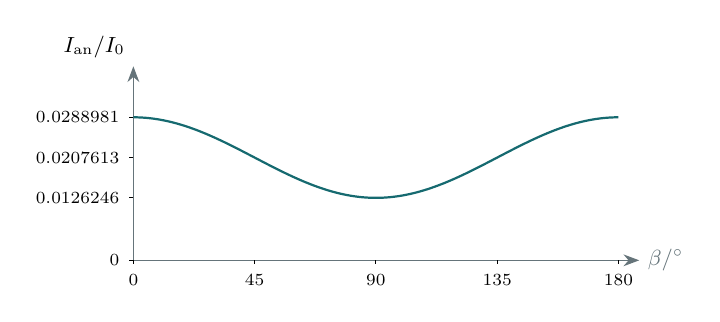
\begin{tikzpicture}[scale=.88,transform shape]
\draw[axis] (0,0.0)--(7.3,0.0) node[right] {$\beta/^\circ$};
\draw[axis] (0,0)--(0,2.8);
\node[above left] at (0,2.8) {$I_{\rm an}/I_0$};
\draw[thin] (0.000000,0.0)--(0.000000,-0.06);\node[below,font=\scriptsize] at (0.000000,-0.08) {$ 0 $};
\draw[thin] (1.750000,0.0)--(1.750000,-0.06);\node[below,font=\scriptsize] at (1.750000,-0.08) {$ 45 $};
\draw[thin] (3.500000,0.0)--(3.500000,-0.06);\node[below,font=\scriptsize] at (3.500000,-0.08) {$ 90 $};
\draw[thin] (5.250000,0.0)--(5.250000,-0.06);\node[below,font=\scriptsize] at (5.250000,-0.08) {$ 135 $};
\draw[thin] (7.000000,0.0)--(7.000000,-0.06);\node[below,font=\scriptsize] at (7.000000,-0.08) {$ 180 $};
\draw[thin] (0,0.000000)--(-.06,0.000000);\node[left,font=\scriptsize] at (-.08,0.000000) {$ 0 $};
\draw[thin] (0,0.901757)--(-.06,0.901757);\node[left,font=\scriptsize] at (-.08,0.901757) {$ 0.0126246 $};
\draw[thin] (0,1.482950)--(-.06,1.482950);\node[left,font=\scriptsize] at (-.08,1.482950) {$ 0.0207613 $};
\draw[thin] (0,2.064150)--(-.06,2.064150);\node[left,font=\scriptsize] at (-.08,2.064150) {$ 0.0288981 $};
\draw[thick,color=accent] plot coordinates {(0.0000000,2.0641466) (0.0291667,2.0639475) (0.0583333,2.0633501) (0.0875000,2.0623550) (0.1166667,2.0609628) (0.1458333,2.0591744) (0.1750000,2.0569911) (0.2041667,2.0544144) (0.2333333,2.0514461) (0.2625000,2.0480881) (0.2916667,2.0443429) (0.3208333,2.0402128) (0.3500000,2.0357009) (0.3791667,2.0308101) (0.4083333,2.0255439) (0.4375000,2.0199057) (0.4666667,2.0138996) (0.4958333,2.0075296) (0.5250000,2.0008001) (0.5541667,1.9937156) (0.5833333,1.9862812) (0.6125000,1.9785017) (0.6416667,1.9703827) (0.6708333,1.9619295) (0.7000000,1.9531481) (0.7291667,1.9440445) (0.7583333,1.9346248) (0.7875000,1.9248956) (0.8166667,1.9148635) (0.8458333,1.9045354) (0.8750000,1.8939183) (0.9041667,1.8830196) (0.9333333,1.8718468) (0.9625000,1.8604073) (0.9916667,1.8487092) (1.0208333,1.8367604) (1.0500000,1.8245692) (1.0791667,1.8121438) (1.1083333,1.7994928) (1.1375000,1.7866248) (1.1666667,1.7735488) (1.1958333,1.7602735) (1.2250000,1.7468083) (1.2541667,1.7331621) (1.2833333,1.7193445) (1.3125000,1.7053649) (1.3416667,1.6912328) (1.3708333,1.6769580) (1.4000000,1.6625503) (1.4291667,1.6480194) (1.4583333,1.6333754) (1.4875000,1.6186284) (1.5166667,1.6037883) (1.5458333,1.5888654) (1.5750000,1.5738700) (1.6041667,1.5588122) (1.6333333,1.5437024) (1.6625000,1.5285510) (1.6916667,1.5133684) (1.7208333,1.4981649) (1.7500000,1.4829509) (1.7791667,1.4677370) (1.8083333,1.4525335) (1.8375000,1.4373508) (1.8666667,1.4221994) (1.8958333,1.4070897) (1.9250000,1.3920319) (1.9541667,1.3770364) (1.9833333,1.3621135) (2.0125000,1.3472735) (2.0416667,1.3325264) (2.0708333,1.3178824) (2.1000000,1.3033516) (2.1291667,1.2889438) (2.1583333,1.2746690) (2.1875000,1.2605370) (2.2166667,1.2465573) (2.2458333,1.2327397) (2.2750000,1.2190936) (2.3041667,1.2056283) (2.3333333,1.1923531) (2.3625000,1.1792770) (2.3916667,1.1664091) (2.4208333,1.1537581) (2.4500000,1.1413327) (2.4791667,1.1291414) (2.5083333,1.1171926) (2.5375000,1.1054945) (2.5666667,1.0940551) (2.5958333,1.0828822) (2.6250000,1.0719835) (2.6541667,1.0613665) (2.6833333,1.0510384) (2.7125000,1.0410063) (2.7416667,1.0312770) (2.7708333,1.0218574) (2.8000000,1.0127537) (2.8291667,1.0039723) (2.8583333,0.9955192) (2.8875000,0.9874001) (2.9166667,0.9796207) (2.9458333,0.9721862) (2.9750000,0.9651018) (3.0041667,0.9583722) (3.0333333,0.9520022) (3.0625000,0.9459961) (3.0916667,0.9403580) (3.1208333,0.9350918) (3.1500000,0.9302010) (3.1791667,0.9256890) (3.2083333,0.9215590) (3.2375000,0.9178137) (3.2666667,0.9144558) (3.2958333,0.9114874) (3.3250000,0.9089107) (3.3541667,0.9067274) (3.3833333,0.9049391) (3.4125000,0.9035469) (3.4416667,0.9025517) (3.4708333,0.9019544) (3.5000000,0.9017552) (3.5291667,0.9019544) (3.5583333,0.9025517) (3.5875000,0.9035469) (3.6166667,0.9049391) (3.6458333,0.9067274) (3.6750000,0.9089107) (3.7041667,0.9114874) (3.7333333,0.9144558) (3.7625000,0.9178137) (3.7916667,0.9215590) (3.8208333,0.9256890) (3.8500000,0.9302010) (3.8791667,0.9350918) (3.9083333,0.9403580) (3.9375000,0.9459961) (3.9666667,0.9520022) (3.9958333,0.9583722) (4.0250000,0.9651018) (4.0541667,0.9721862) (4.0833333,0.9796207) (4.1125000,0.9874001) (4.1416667,0.9955192) (4.1708333,1.0039723) (4.2000000,1.0127537) (4.2291667,1.0218574) (4.2583333,1.0312770) (4.2875000,1.0410063) (4.3166667,1.0510384) (4.3458333,1.0613665) (4.3750000,1.0719835) (4.4041667,1.0828822) (4.4333333,1.0940551) (4.4625000,1.1054945) (4.4916667,1.1171926) (4.5208333,1.1291414) (4.5500000,1.1413327) (4.5791667,1.1537581) (4.6083333,1.1664091) (4.6375000,1.1792770) (4.6666667,1.1923531) (4.6958333,1.2056283) (4.7250000,1.2190936) (4.7541667,1.2327397) (4.7833333,1.2465573) (4.8125000,1.2605370) (4.8416667,1.2746690) (4.8708333,1.2889438) (4.9000000,1.3033516) (4.9291667,1.3178824) (4.9583333,1.3325264) (4.9875000,1.3472735) (5.0166667,1.3621135) (5.0458333,1.3770364) (5.0750000,1.3920319) (5.1041667,1.4070897) (5.1333333,1.4221994) (5.1625000,1.4373508) (5.1916667,1.4525335) (5.2208333,1.4677370) (5.2500000,1.4829509) (5.2791667,1.4981649) (5.3083333,1.5133684) (5.3375000,1.5285510) (5.3666667,1.5437024) (5.3958333,1.5588122) (5.4250000,1.5738700) (5.4541667,1.5888654) (5.4833333,1.6037883) (5.5125000,1.6186284) (5.5416667,1.6333754) (5.5708333,1.6480194) (5.6000000,1.6625503) (5.6291667,1.6769580) (5.6583333,1.6912328) (5.6875000,1.7053649) (5.7166667,1.7193445) (5.7458333,1.7331621) (5.7750000,1.7468083) (5.8041667,1.7602735) (5.8333333,1.7735488) (5.8625000,1.7866248) (5.8916667,1.7994928) (5.9208333,1.8121438) (5.9500000,1.8245692) (5.9791667,1.8367604) (6.0083333,1.8487092) (6.0375000,1.8604073) (6.0666667,1.8718468) (6.0958333,1.8830196) (6.1250000,1.8939183) (6.1541667,1.9045354) (6.1833333,1.9148635) (6.2125000,1.9248956) (6.2416667,1.9346248) (6.2708333,1.9440445) (6.3000000,1.9531481) (6.3291667,1.9619295) (6.3583333,1.9703827) (6.3875000,1.9785017) (6.4166667,1.9862812) (6.4458333,1.9937156) (6.4750000,2.0008001) (6.5041667,2.0075296) (6.5333333,2.0138996) (6.5625000,2.0199057) (6.5916667,2.0255439) (6.6208333,2.0308101) (6.6500000,2.0357009) (6.6791667,2.0402128) (6.7083333,2.0443429) (6.7375000,2.0480881) (6.7666667,2.0514461) (6.7958333,2.0544144) (6.8250000,2.0569911) (6.8541667,2.0591744) (6.8833333,2.0609628) (6.9125000,2.0623550) (6.9416667,2.0633501) (6.9708333,2.0639475) (7.0000000,2.0641466)};
\end{tikzpicture}
\figcaption{解图光4.5C\quad 固定30度入射后旋转检偏，轴角相对s定义}
\end{minipage}\end{center}

\textbf{等效自然光与线偏振光。}将图A两柱的共同部分各取$I_p$，它们合成总强度$I_n=2I_p=0.0252491I_0$的自然光；$s$方向多出的部分为$I_\ell=I_s-I_p=0.0162735I_0$的线偏振光。图D列出这两份与反射总强度，满足$I_n+I_\ell=I_R$，且$P_L=I_\ell/I_R$。该比例描述反射束内部的不平衡；总反射功率比例$\mathcal R=I_R/I_0=0.0415226$描述入射能量中被反射的份额。

\begin{center}\begin{minipage}{.98\linewidth}\centering
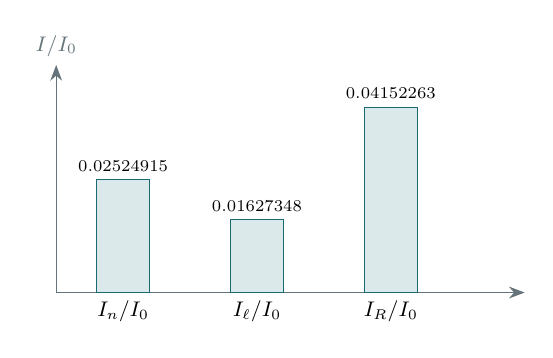
\begin{tikzpicture}[scale=.85,transform shape]
\draw[axis] (0,0)--(7,0); \draw[axis] (0,0)--(0,3.4) node[above] {$I/I_0$};
\filldraw[fill=accent!15,draw=accent] (0.6,0) rectangle (1.4,1.6832764);\node[above,font=\scriptsize] at (1,1.6832764) {$ 0.02524915 $};\node[below] at (1,0) {$I_n/I_0$};
\filldraw[fill=accent!15,draw=accent] (2.6,0) rectangle (3.4,1.0848986);\node[above,font=\scriptsize] at (3,1.0848986) {$ 0.01627348 $};\node[below] at (3,0) {$I_\ell/I_0$};
\filldraw[fill=accent!15,draw=accent] (4.6,0) rectangle (5.4,2.7681751);\node[above,font=\scriptsize] at (5,2.7681751) {$ 0.04152263 $};\node[below] at (5,0) {$I_R/I_0$};
\end{tikzpicture}
\figcaption{解图光4.5D\quad 等效自然背景与线偏部分相加恢复反射总强度}
\end{minipage}\end{center}

上述分解来自反射场的相干矩阵。按$(p,s)$顺序，
\[
\mathsf J_r=\frac{I_0}{2}
\begin{pmatrix}R_p&0\\0&R_s\end{pmatrix}.
\]
入射互相关为零，分别乘Fresnel振幅后仍为零，所以反射束只有线偏振统计量、圆偏振分量为零。$r_s$的负号给该局部电场共同的相位反向，两个互不相干分量的强度按$|r_j|^2$计算。若换成45°线偏振输入，其反射两对角强度仍为$I_0R_p/2,I_0R_s/2$，互相关则为$I_0r_pr_s/2$。两个实分量具有固定相位关系，构成完全线偏振反射光；自然光对应的互相关为零。

本题30°小于布儒斯特角$\arctan1.50=56.3099^\circ$，$p$反射保持非零；在布儒斯特角才得到只有$s$分量的反射束。透明界面还满足每个偏振端口的$\mathcal R_j+\mathcal T_j=1$，可由此计算同一入射束的透射结果。


\Needspace{13\baselineskip}

\pdfbookmark[2]{第 6 题 布儒斯特入射的振幅、强度与功率}{q6}

\section*{第 6 题\quad 布儒斯特入射的振幅、强度与功率}\label{q:6}

自然光从空气射入折射率为1.50的玻璃，入射角为布儒斯特角。分别求$s,p$分量的振幅反射、透射系数，单位垂直光线截面的强度比，以及整束光的功率反射、透射比。再求透射光的线偏振度。

\begin{center}\begin{minipage}{.98\linewidth}\centering
\begin{tikzpicture}[scale=.9,transform shape]
\draw[object] (-3.10000,0.00000)--(3.50000,0.00000);\draw[guide] (0.00000,-2.50000)--(0.00000,2.70000);\fill (0.00000,0.00000) circle(.035);\node[above right] at (0.00000,0.00000) {$O$};\draw[motion] (-2.08013,1.38675)--(0.00000,0.00000);
\draw[motion] (0.00000,0.00000)--(2.08013,1.38675);\draw[motion] (0.00000,0.00000)--(1.38675,-2.08013);\node[right] at (-2.90000,1.50000) {$n_1$};\node[right] at (-2.90000,-1.50000) {$n_2$};\node[left] at (-0.50000,1.00000) {$\theta_i$};\node[right] at (0.55000,1.10000) {$\theta_r$};\node[right] at (0.42000,-1.00000) {$\theta_t$};\node[above] at (-2.80000,2.40000) {布儒斯特入射};
\end{tikzpicture}
\figcaption{图光4.6\quad 布儒斯特角下的界面与折射束}
\end{minipage}\end{center}

\Needspace{6\baselineskip}\subsection*{解答}


\textbf{先固定角度和振幅定义。}取空气折射率为1，玻璃折射率$n=3/2$，界面无吸收、两介质非磁性。各束的$s$方向垂直入射面，$p$方向在入射面内并随传播方向定义。布儒斯特条件给
\[
\tan\theta_B=\frac32,\quad
\cos\theta_B=\frac2{\sqrt{13}},\quad
\cos\theta_t=\frac3{\sqrt{13}},\quad
\theta_t=\frac\pi2-\theta_B .
\]
因此$\theta_B=56.3099^\circ$、$\theta_t=33.6901^\circ$。记$c_i=\cos\theta_B,c_t=\cos\theta_t$，空气到玻璃的Fresnel振幅式为
\[
r_s=\frac{c_i-nc_t}{c_i+nc_t},\quad t_s=\frac{2c_i}{c_i+nc_t},\qquad
r_p=\frac{nc_i-c_t}{nc_i+c_t},\quad t_p=\frac{2c_i}{nc_i+c_t}.
\]
将精确余弦代入，$s$系数分别为$(2-9/2)/(2+9/2)$和$4/(2+9/2)$，$p$反射分子为零，得到
\[
\boxed{r_s=-\frac5{13},\quad r_p=0,\quad t_s=\frac8{13},\quad t_p=\frac23}.
\]

\textbf{局部光强来自能流密度。}对非磁性介质平面波，$\boldsymbol H=(n/\mu_0c)\hat{\boldsymbol k}\times\boldsymbol E$，时间平均坡印廷矢量沿传播方向，大小为
\[
I=\frac12\operatorname{Re}(\boldsymbol E\times\boldsymbol H^*)\cdot\hat{\boldsymbol k}
=\frac{n}{2\mu_0c}|E|^2
=\frac{n\varepsilon_0c}{2}|E|^2 .
\]
光强也可写作$I=\tfrac12\sqrt{\varepsilon/\mu}|E|^2$；在本模型中$\mu=\mu_0$、$n=\sqrt{\varepsilon_r}$，与上式一致。复振幅$E$采用峰值约定，时间平均给出共同的$1/2$。这里的$I$以垂直光线的单位截面积计。反射和入射在同一空气介质，强度反射率为$R_s=25/169,R_p=0$；透射进入玻璃，局部强度比为
\[
T_s^{(I)}=n|t_s|^2=\frac{96}{169}=0.568047,
\quad T_p^{(I)}=n|t_p|^2=\frac23.
\]

\textbf{同一界面足迹给整束功率。}图A用$A_\Sigma$表示界面上的共同光束足迹。它在入射、透射光线法向平面上的投影为
\[
A_i=A_\Sigma\cos\theta_B,\qquad
A_t=A_\Sigma\cos\theta_t,\qquad
\frac{A_t}{A_i}=\frac32.
\]
在界面上，坡印廷矢量的法向分量为$I\cos\theta$；通过同一界面足迹的功率等于该法向分量乘$A_\Sigma$。它与先取光线法向强度再乘$A_i,A_t$是同一个投影关系。因此每个偏振的总功率透射比为
\[
\mathcal T_j=\frac{I_{t,j}A_t}{I_{i,j}A_i}
=\frac{n\cos\theta_t}{\cos\theta_B}|t_j|^2.
\]

\begin{center}\begin{minipage}{.98\linewidth}\centering
\begin{tikzpicture}[scale=.68,transform shape]
\draw[object] (-3.10000,0.00000)--(3.50000,0.00000);\draw[guide] (0.00000,-2.50000)--(0.00000,2.70000);\fill (0.00000,0.00000) circle(.035);\node[above right] at (0.00000,0.00000) {$O$};\draw[motion] (-2.08013,1.38675)--(0.00000,0.00000);
\draw[motion] (0.00000,0.00000)--(2.08013,1.38675);\draw[motion] (0.00000,0.00000)--(1.38675,-2.08013);\node[right] at (-2.90000,1.50000) {$n_1$};\node[right] at (-2.90000,-1.50000) {$n_2$};\node[left] at (-0.50000,1.00000) {$\theta_i$};\node[right] at (0.55000,1.10000) {$\theta_r$};\node[right] at (0.42000,-1.00000) {$\theta_t$};\node[above] at (-2.80000,2.40000) {布儒斯特入射};\begin{scope}[shift={(6.00000,1.50000)}]
\node[above right] at (0.00000,0.40000) {透射量};\node[above right] at (2.60000,0.40000) {$s$};\node[above right] at (5.30000,0.40000) {$p$};\draw[thin] (-0.20000,0.10000)--(10.20000,0.10000);\node[above right] at (0.00000,-0.48000) {振幅};\node[above right] at (2.60000,-0.48000) {$t_s=8/13$};\node[above right] at (5.30000,-0.48000) {$t_p=2/3$};\node[above right] at (0.00000,-1.11000) {局部强度};\node[above right] at (2.60000,-1.11000) {$96/169$};\node[above right] at (5.30000,-1.11000) {$2/3$};\node[above right] at (0.00000,-1.74000) {整束功率};\node[above right] at (2.60000,-1.74000) {$144/169$};\node[above right] at (5.30000,-1.74000) {$1$};
\end{scope}\draw[very thick,color=accent] (-0.50000,0.00000)--(0.50000,0.00000);\node[right] at (0.80000,0.10000) {$A_\Sigma$};\node[below] at (6.00000,-2.00000) {$A_t/A_i=\cos\theta_t/\cos\theta_B$};\draw[very thick,color=accent] (-1.40192,0.60128)--(-1.09423,1.06282);\node[above left] at (-1.10940,1.04006) {$A_i$};\draw[very thick,color=accent] (0.48590,-1.47884)--(1.17820,-1.01731);\node[below right] at (1.04006,-1.10940) {$A_t$};
\end{tikzpicture}
\figcaption{解图光4.6A\quad 共同足迹投影与三种透射系数}
\end{minipage}\end{center}

代入几何比和振幅系数，得到
\[
\boxed{\mathcal R_s=\frac{25}{169},\quad\mathcal T_s=\frac{144}{169},
\quad\mathcal R_p=0,\quad\mathcal T_p=1}.
\]
两偏振分别有$\mathcal R_j+\mathcal T_j=1$。例如$s$的局部强度比之和为$25/169+96/169=121/169$，相同界面足迹对应的功率比之和为$25/169+144/169=1$；所用截面积的区别正由图A的投影关系给出。图B把局部强度透射比与整束功率透射比按标签分列。

\begin{center}\begin{minipage}{.98\linewidth}\centering
\begin{tikzpicture}[scale=.85,transform shape]
\draw[axis] (0,0)--(9,0); \draw[axis] (0,0)--(0,3.4) node[above] {$\text{相应比值}$};
\filldraw[fill=accent!15,draw=accent] (0.6,0) rectangle (1.4,1.6229924);\node[above,font=\scriptsize] at (1,1.6229924) {$ 0.5680473 $};\node[below] at (1,0) {$T_s^{(I)}$};
\filldraw[fill=accent!15,draw=accent] (2.6,0) rectangle (3.4,1.9047619);\node[above,font=\scriptsize] at (3,1.9047619) {$ 0.6666667 $};\node[below] at (3,0) {$T_p^{(I)}$};
\filldraw[fill=accent!15,draw=accent] (4.6,0) rectangle (5.4,2.4344886);\node[above,font=\scriptsize] at (5,2.4344886) {$ 0.852071 $};\node[below] at (5,0) {$\mathcal T_s$};
\filldraw[fill=accent!15,draw=accent] (6.6,0) rectangle (7.4,2.8571429);\node[above,font=\scriptsize] at (7,2.8571429) {$ 1 $};\node[below] at (7,0) {$\mathcal T_p$};
\end{tikzpicture}
\figcaption{解图光4.6B\quad 局部强度比与整束功率比按各自定义列出}
\end{minipage}\end{center}

\textbf{自然入射的两个输出端。}入射自然光在$s,p$方向各占一半功率，且两分量互不相干。反射只保留$s$分量，因此反射束完全线偏振；总反射、透射功率比例为
\[
\mathcal R=\frac12\frac{25}{169}=\frac{25}{338},\qquad
\mathcal T=\frac12\left(\frac{144}{169}+1\right)=\frac{313}{338}.
\]
图C分列四个偏振端口，功率总和恢复入射功率。自然光入射的互相关为零，透射后两个分量仍互不相干，圆偏振统计量为零；本题的线偏振度因此也等于总偏振度。透射中$p$较强，按本束两分量的差商得
\[
\boxed{P_{L,t}=\frac{\mathcal T_p-\mathcal T_s}{\mathcal T_p+\mathcal T_s}
=\frac{25}{313}=0.0798722\simeq7.99\%}.
\]

\begin{center}\begin{minipage}{.98\linewidth}\centering
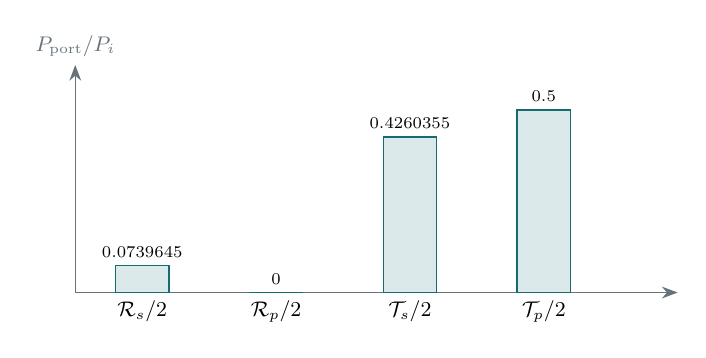
\begin{tikzpicture}[scale=.85,transform shape]
\draw[axis] (0,0)--(9,0); \draw[axis] (0,0)--(0,3.4) node[above] {$P_{\rm port}/P_i$};
\filldraw[fill=accent!15,draw=accent] (0.6,0) rectangle (1.4,0.4034427);\node[above,font=\scriptsize] at (1,0.4034427) {$ 0.0739645 $};\node[below] at (1,0) {$\mathcal R_s/2$};
\filldraw[fill=accent!15,draw=accent] (2.6,0) rectangle (3.4,0.0000000);\node[above,font=\scriptsize] at (3,0.0000000) {$ 0 $};\node[below] at (3,0) {$\mathcal R_p/2$};
\filldraw[fill=accent!15,draw=accent] (4.6,0) rectangle (5.4,2.3238300);\node[above,font=\scriptsize] at (5,2.3238300) {$ 0.4260355 $};\node[below] at (5,0) {$\mathcal T_s/2$};
\filldraw[fill=accent!15,draw=accent] (6.6,0) rectangle (7.4,2.7272727);\node[above,font=\scriptsize] at (7,2.7272727) {$ 0.5 $};\node[below] at (7,0) {$\mathcal T_p/2$};
\end{tikzpicture}
\figcaption{解图光4.6C\quad 自然入射的四个偏振端口功率相加为1}
\end{minipage}\end{center}

同一透射束内两偏振共享截面积和介质系数，故用局部强度或整束功率求偏振度得到同一结果。其总局部强度比为$I_t/I_i=(96/169+2/3)/2=313/507$，乘$A_t/A_i=3/2$后才成为整束功率比$313/338$。振幅由界面场决定，局部强度由$n|E|^2$决定，整束功率再乘实际束截面积；三种比值依次由这些关系得到。

图D将材料折射率作为参数，在同样的空气入射布儒斯特模型下绘出透射线偏振度。$n=1.50$处只有约7.99\%，对应大量$s$功率仍透过的具体比例；反射端的纯$s$与透射端的两分量共存由同一组端口系数确定。

\begin{center}\begin{minipage}{.98\linewidth}\centering
\begin{tikzpicture}[scale=.88,transform shape]
\draw[axis] (0,0.0)--(7.3,0.0) node[right] {$n$};
\draw[axis] (0,0)--(0,2.8);
\node[above left] at (0,2.8) {$P_{L,t}$};
\draw[thin] (0.000000,0.0)--(0.000000,-0.06);\node[below,font=\scriptsize] at (0.000000,-0.08) {$ 1 $};
\draw[thin] (1.166667,0.0)--(1.166667,-0.06);\node[below,font=\scriptsize] at (1.166667,-0.08) {$ 1.5 $};
\draw[thin] (2.333333,0.0)--(2.333333,-0.06);\node[below,font=\scriptsize] at (2.333333,-0.08) {$ 2 $};
\draw[thin] (4.666667,0.0)--(4.666667,-0.06);\node[below,font=\scriptsize] at (4.666667,-0.08) {$ 3 $};
\draw[thin] (7.000000,0.0)--(7.000000,-0.06);\node[below,font=\scriptsize] at (7.000000,-0.08) {$ 4 $};
\draw[thin] (0,0.000000)--(-.06,0.000000);\node[left,font=\scriptsize] at (-.08,0.000000) {$ 0 $};
\draw[thin] (0,0.285258)--(-.06,0.285258);\node[left,font=\scriptsize] at (-.08,0.285258) {$ 0.0798722 $};
\draw[thin] (0,1.071429)--(-.06,1.071429);\node[left,font=\scriptsize] at (-.08,1.071429) {$ 0.3 $};
\draw[thin] (0,1.785714)--(-.06,1.785714);\node[left,font=\scriptsize] at (-.08,1.785714) {$ 0.5 $};
\draw[thin] (0,2.321429)--(-.06,2.321429);\node[left,font=\scriptsize] at (-.08,2.321429) {$ 0.65 $};
\draw[thick,color=accent] plot coordinates {(0.0000000,0.0000000) (0.0291667,0.0002756) (0.0583333,0.0010887) (0.0875000,0.0024196) (0.1166667,0.0042492) (0.1458333,0.0065591) (0.1750000,0.0093316) (0.2041667,0.0125497) (0.2333333,0.0161969) (0.2625000,0.0202572) (0.2916667,0.0247155) (0.3208333,0.0295568) (0.3500000,0.0347670) (0.3791667,0.0403323) (0.4083333,0.0462393) (0.4375000,0.0524753) (0.4666667,0.0590278) (0.4958333,0.0658850) (0.5250000,0.0730351) (0.5541667,0.0804670) (0.5833333,0.0881700) (0.6125000,0.0961335) (0.6416667,0.1043474) (0.6708333,0.1128021) (0.7000000,0.1214879) (0.7291667,0.1303958) (0.7583333,0.1395170) (0.7875000,0.1488427) (0.8166667,0.1583648) (0.8458333,0.1680752) (0.8750000,0.1779662) (0.9041667,0.1880301) (0.9333333,0.1982597) (0.9625000,0.2086480) (0.9916667,0.2191880) (1.0208333,0.2298732) (1.0500000,0.2406971) (1.0791667,0.2516534) (1.1083333,0.2627362) (1.1375000,0.2739396) (1.1666667,0.2852579) (1.1958333,0.2966855) (1.2250000,0.3082172) (1.2541667,0.3198478) (1.2833333,0.3315722) (1.3125000,0.3433856) (1.3416667,0.3552832) (1.3708333,0.3672606) (1.4000000,0.3793131) (1.4291667,0.3914366) (1.4583333,0.4036267) (1.4875000,0.4158796) (1.5166667,0.4281912) (1.5458333,0.4405578) (1.5750000,0.4529755) (1.6041667,0.4654409) (1.6333333,0.4779504) (1.6625000,0.4905007) (1.6916667,0.5030884) (1.7208333,0.5157105) (1.7500000,0.5283638) (1.7791667,0.5410453) (1.8083333,0.5537521) (1.8375000,0.5664814) (1.8666667,0.5792305) (1.8958333,0.5919967) (1.9250000,0.6047774) (1.9541667,0.6175702) (1.9833333,0.6303727) (2.0125000,0.6431825) (2.0416667,0.6559973) (2.0708333,0.6688150) (2.1000000,0.6816334) (2.1291667,0.6944505) (2.1583333,0.7072642) (2.1875000,0.7200727) (2.2166667,0.7328740) (2.2458333,0.7456663) (2.2750000,0.7584479) (2.3041667,0.7712170) (2.3333333,0.7839721) (2.3625000,0.7967115) (2.3916667,0.8094337) (2.4208333,0.8221372) (2.4500000,0.8348206) (2.4791667,0.8474824) (2.5083333,0.8601213) (2.5375000,0.8727360) (2.5666667,0.8853253) (2.5958333,0.8978879) (2.6250000,0.9104227) (2.6541667,0.9229285) (2.6833333,0.9354042) (2.7125000,0.9478488) (2.7416667,0.9602612) (2.7708333,0.9726405) (2.8000000,0.9849858) (2.8291667,0.9972961) (2.8583333,1.0095705) (2.8875000,1.0218083) (2.9166667,1.0340085) (2.9458333,1.0461704) (2.9750000,1.0582933) (3.0041667,1.0703765) (3.0333333,1.0824191) (3.0625000,1.0944207) (3.0916667,1.1063806) (3.1208333,1.1182980) (3.1500000,1.1301726) (3.1791667,1.1420036) (3.2083333,1.1537906) (3.2375000,1.1655331) (3.2666667,1.1772305) (3.2958333,1.1888825) (3.3250000,1.2004885) (3.3541667,1.2120481) (3.3833333,1.2235610) (3.4125000,1.2350268) (3.4416667,1.2464451) (3.4708333,1.2578155) (3.5000000,1.2691378) (3.5291667,1.2804116) (3.5583333,1.2916367) (3.5875000,1.3028128) (3.6166667,1.3139396) (3.6458333,1.3250169) (3.6750000,1.3360445) (3.7041667,1.3470221) (3.7333333,1.3579497) (3.7625000,1.3688269) (3.7916667,1.3796537) (3.8208333,1.3904299) (3.8500000,1.4011554) (3.8791667,1.4118300) (3.9083333,1.4224536) (3.9375000,1.4330262) (3.9666667,1.4435476) (3.9958333,1.4540178) (4.0250000,1.4644367) (4.0541667,1.4748043) (4.0833333,1.4851205) (4.1125000,1.4953853) (4.1416667,1.5055987) (4.1708333,1.5157606) (4.2000000,1.5258711) (4.2291667,1.5359301) (4.2583333,1.5459378) (4.2875000,1.5558940) (4.3166667,1.5657988) (4.3458333,1.5756524) (4.3750000,1.5854546) (4.4041667,1.5952057) (4.4333333,1.6049055) (4.4625000,1.6145543) (4.4916667,1.6241521) (4.5208333,1.6336989) (4.5500000,1.6431949) (4.5791667,1.6526401) (4.6083333,1.6620347) (4.6375000,1.6713787) (4.6666667,1.6806723) (4.6958333,1.6899155) (4.7250000,1.6991086) (4.7541667,1.7082516) (4.7833333,1.7173447) (4.8125000,1.7263880) (4.8416667,1.7353816) (4.8708333,1.7443257) (4.9000000,1.7532204) (4.9291667,1.7620660) (4.9583333,1.7708624) (4.9875000,1.7796100) (5.0166667,1.7883088) (5.0458333,1.7969591) (5.0750000,1.8055610) (5.1041667,1.8141147) (5.1333333,1.8226203) (5.1625000,1.8310780) (5.1916667,1.8394881) (5.2208333,1.8478507) (5.2500000,1.8561660) (5.2791667,1.8644341) (5.3083333,1.8726553) (5.3375000,1.8808298) (5.3666667,1.8889578) (5.3958333,1.8970394) (5.4250000,1.9050749) (5.4541667,1.9130644) (5.4833333,1.9210082) (5.5125000,1.9289065) (5.5416667,1.9367594) (5.5708333,1.9445672) (5.6000000,1.9523302) (5.6291667,1.9600484) (5.6583333,1.9677221) (5.6875000,1.9753516) (5.7166667,1.9829370) (5.7458333,1.9904786) (5.7750000,1.9979765) (5.8041667,2.0054311) (5.8333333,2.0128424) (5.8625000,2.0202108) (5.8916667,2.0275364) (5.9208333,2.0348195) (5.9500000,2.0420602) (5.9791667,2.0492589) (6.0083333,2.0564157) (6.0375000,2.0635308) (6.0666667,2.0706045) (6.0958333,2.0776370) (6.1250000,2.0846285) (6.1541667,2.0915792) (6.1833333,2.0984893) (6.2125000,2.1053592) (6.2416667,2.1121889) (6.2708333,2.1189787) (6.3000000,2.1257289) (6.3291667,2.1324397) (6.3583333,2.1391112) (6.3875000,2.1457437) (6.4166667,2.1523375) (6.4458333,2.1588926) (6.4750000,2.1654095) (6.5041667,2.1718882) (6.5333333,2.1783291) (6.5625000,2.1847322) (6.5916667,2.1910980) (6.6208333,2.1974264) (6.6500000,2.2037179) (6.6791667,2.2099725) (6.7083333,2.2161906) (6.7375000,2.2223723) (6.7666667,2.2285178) (6.7958333,2.2346274) (6.8250000,2.2407013) (6.8541667,2.2467397) (6.8833333,2.2527427) (6.9125000,2.2587107) (6.9416667,2.2646438) (6.9708333,2.2705423) (7.0000000,2.2764063)};
\end{tikzpicture}
\figcaption{解图光4.6D\quad 空气到透明介质的布儒斯特透射线偏振度}
\end{minipage}\end{center}


\Needspace{13\baselineskip}

\pdfbookmark[2]{第 7 题 玻璃片堆的偏振选择}{q7}

\section*{第 7 题\quad 玻璃片堆的偏振选择}\label{q:7}

自然光依次通过若干相同的平行玻璃片，每片折射率为1.54，放置角使光在各空气—玻璃界面均满足布儒斯特条件。忽略吸收和片内多次反射，只收集主透射光束。求通过1、2、4片后的线偏振度；至少需多少片使偏振度达到99\%。

\begin{center}\begin{minipage}{.98\linewidth}\centering
\begin{tikzpicture}[scale=.9,transform shape]
\draw[object] (-0.7090763,-0.4109296)--(0.6328315,0.4604391)--(0.7090763,0.3430222)--(-0.6328315,-0.5283465)--cycle;
\draw[motion] (-1.0000000,0.0000000)--(-0.0762448,0.0000000);\draw[motion] (-0.0762448,0.0000000)--(0.0762448,-0.0679073);
\node[above] at (0.0000000,0.8660463) {玻璃$1$};
\node[below] at (0.0000000,-0.8839537) {两界面};
\draw[object] (1.2909237,-0.4788369)--(2.6328315,0.3925318)--(2.7090763,0.2751149)--(1.3671685,-0.5962538)--cycle;
\draw[motion] (0.0762448,-0.0679073)--(1.9237552,-0.0679073);\draw[motion] (1.9237552,-0.0679073)--(2.0762448,-0.1358147);
\node[above] at (2.0000000,0.7981390) {玻璃$2$};
\node[below] at (2.0000000,-0.9518610) {两界面};
\draw[object] (3.2909237,-0.5467443)--(4.6328315,0.3246245)--(4.7090763,0.2072075)--(3.3671685,-0.6641612)--cycle;
\draw[motion] (2.0762448,-0.1358147)--(3.9237552,-0.1358147);\draw[motion] (3.9237552,-0.1358147)--(4.0762448,-0.2037220);
\node[above] at (4.0000000,0.7302316) {玻璃$\cdots$};
\node[below] at (4.0000000,-1.0197684) {两界面};
\draw[object] (5.2909237,-0.6146516)--(6.6328315,0.2567171)--(6.7090763,0.1393002)--(5.3671685,-0.7320685)--cycle;
\draw[motion] (4.0762448,-0.2037220)--(5.9237552,-0.2037220);\draw[motion] (5.9237552,-0.2037220)--(6.0762448,-0.2716294);
\node[above] at (6.0000000,0.6623243) {玻璃$N$};
\node[below] at (6.0000000,-1.0876757) {两界面};
\draw[motion] (6.0762448,-0.2716294)--(7.2000000,-0.2716294);
\end{tikzpicture}
\figcaption{图光4.7\quad 同向倾斜玻璃片内的折射与片后平行主束}
\end{minipage}\end{center}

\Needspace{6\baselineskip}\subsection*{解答}


图光4.7的所有玻璃片有共同的入射面。取$p$轴在此面内、$s$轴垂直此面，入射自然光的两分量互不相干，功率各为$P_0/2$。每片只跟踪依次穿过两个面的主透射束。片前、片后的介质同为空气，出射方向平行于入射方向，整束截面积也相同，因而整片的功率比等于整片振幅比的模平方。

由$n=1.54$及布儒斯特条件，图中外部、内部角分别为
\[
\theta_B=\arctan n=57.0023^\circ,\qquad
\theta_t=90^\circ-\theta_B=32.9977^\circ,
\quad \sin\theta_B=n\sin\theta_t.
\]
两个传播方向的$p$反射振幅均为零。$s$反射振幅在第一面为$(1-n^2)/(1+n^2)$，在第二面反号，故两面的$s$功率透射率相同：
\[
q=1-\left(\frac{n^2-1}{n^2+1}\right)^2
=\frac{4n^2}{(1+n^2)^2}=0.834505768.
\]
解图光4.7A的每一小段表示穿过一个面，$p$功率保持原值，$s$功率乘$q$。从振幅也能直接看出一片中两面的作用。菲涅耳透射式给出
\[
 t_s^{(1)}=\frac{2\sin\theta_t\cos\theta_B}{\sin(\theta_B+\theta_t)}
 =\frac{2}{1+n^2},\qquad
 t_s^{(2)}=\frac{2\sin\theta_B\cos\theta_t}{\sin(\theta_B+\theta_t)}
 =\frac{2n^2}{1+n^2}.
\]
因此一片$s$振幅乘$t_s^{(1)}t_s^{(2)}=4n^2/(1+n^2)^2=q$，$p$振幅乘$(1/n)n=1$。这里$q$既是一个面的功率比，也恰好等于一整片的$s$振幅比；一片的$s$功率比为$q^2$。单面的功率换算含折射率与截面积因子；一整片的输入、输出同在空气中，两个互易界面的这些因子相消。
\begin{center}\begin{minipage}{.98\linewidth}\centering
\begin{tikzpicture}[scale=.9,transform shape]
\fill (0.00000,1.00000) circle(.035);\node[above] at (0.00000,1.30000) {$p$不变};\fill (0.00000,-0.30000) circle(.035);\node[below] at (0.00000,-0.70000) {$q^{0}$};\draw[motion] (0.00000,1.00000)--(2.00000,1.00000);\draw[motion] (0.00000,-0.30000)--(2.00000,-0.58000);\fill (2.00000,1.00000) circle(.035);\node[above] at (2.00000,1.30000) {$1$};\fill (2.00000,-0.58000) circle(.035);\node[below] at (2.00000,-0.98000) {$q^{1}$};\draw[motion] (2.00000,1.00000)--(4.00000,1.00000);\draw[motion] (2.00000,-0.58000)--(4.00000,-0.86000);\fill (4.00000,1.00000) circle(.035);\node[above] at (4.00000,1.30000) {$1$};\fill (4.00000,-0.86000) circle(.035);\node[below] at (4.00000,-1.26000) {$q^{2}$};\draw[motion] (4.00000,1.00000)--(6.00000,1.00000);\draw[motion] (4.00000,-0.86000)--(6.00000,-1.14000);\fill (6.00000,1.00000) circle(.035);\node[above] at (6.00000,1.30000) {$1$};\fill (6.00000,-1.14000) circle(.035);\node[below] at (6.00000,-1.54000) {$q^{3}$};\draw[motion] (6.00000,1.00000)--(8.00000,1.00000);\draw[motion] (6.00000,-1.14000)--(8.00000,-1.42000);\fill (8.00000,1.00000) circle(.035);\node[above] at (8.00000,1.30000) {$1$};\fill (8.00000,-1.42000) circle(.035);\node[below] at (8.00000,-1.82000) {$q^{4}$};\node[above] at (4.00000,2.00000) {每个界面一次选择；每片含两个界面};\node[below] at (4.00000,-2.50000) {$P_{L,14}=98.746\%<99\%<P_{L,15}=99.125\%$};
\end{tikzpicture}
\figcaption{解图光4.7A\quad 逐界面功率链与整数片数检查}
\end{minipage}\end{center}
连续通过两片、四片时，$s$振幅分别乘$q^2=0.696399876$、$q^4=0.484972788$；$s$功率分别乘$q^4$、$q^8$。一般地，$N$片有$2N$个面，故
\[
P_{p,N}=P_0/2,\qquad P_{s,N}=P_0q^{2N}/2,
\quad\boxed{P_{L,N}=\frac{1-q^{2N}}{1+q^{2N}}}.
\]
上式偏振度取沿$p,s$方向通过理想检偏器所得最大、最小功率之差与和的比值。两分量互不相干，交叉平均为零，且$q^{2N}\leqslant1$，所以最大功率沿$p$轴。解图光4.7B把两分量功率直接画在同一纵轴上，偏振度正是两曲线高度之差与和的比值。
\begin{center}\begin{minipage}{.98\linewidth}\centering
\begin{tikzpicture}[scale=.88,transform shape]
\draw[axis] (0,0.0)--(7.3,0.0) node[right] {$N$};
\draw[axis] (0,0)--(0,2.8);
\node[above left] at (0,2.8) {$P_j/P_0$};
\draw[thin] (0.000000,0.0)--(0.000000,-0.06);\node[below,font=\scriptsize] at (0.000000,-0.08) {$ 0 $};
\draw[thin] (0.437500,0.0)--(0.437500,-0.06);\node[below,font=\scriptsize] at (0.437500,-0.08) {$ 1 $};
\draw[thin] (0.875000,0.0)--(0.875000,-0.06);\node[below,font=\scriptsize] at (0.875000,-0.08) {$ 2 $};
\draw[thin] (1.750000,0.0)--(1.750000,-0.06);\node[below,font=\scriptsize] at (1.750000,-0.08) {$ 4 $};
\draw[thin] (3.500000,0.0)--(3.500000,-0.06);\node[below,font=\scriptsize] at (3.500000,-0.08) {$ 8 $};
\draw[thin] (5.250000,0.0)--(5.250000,-0.06);\node[below,font=\scriptsize] at (5.250000,-0.08) {$ 12 $};
\draw[thin] (7.000000,0.0)--(7.000000,-0.06);\node[below,font=\scriptsize] at (7.000000,-0.08) {$ 16 $};
\draw[thin] (0,0.000000)--(-.06,0.000000);\node[left,font=\scriptsize] at (-.08,0.000000) {$ 0 $};
\draw[thin] (0,1.136364)--(-.06,1.136364);\node[left,font=\scriptsize] at (-.08,1.136364) {$ 0.25 $};
\draw[thin] (0,2.272727)--(-.06,2.272727);\node[left,font=\scriptsize] at (-.08,2.272727) {$ 0.5 $};
\draw[thick,color=accent] plot coordinates {(0.0000000,2.2727273) (0.0291667,2.2727273) (0.0583333,2.2727273) (0.0875000,2.2727273) (0.1166667,2.2727273) (0.1458333,2.2727273) (0.1750000,2.2727273) (0.2041667,2.2727273) (0.2333333,2.2727273) (0.2625000,2.2727273) (0.2916667,2.2727273) (0.3208333,2.2727273) (0.3500000,2.2727273) (0.3791667,2.2727273) (0.4083333,2.2727273) (0.4375000,2.2727273) (0.4666667,2.2727273) (0.4958333,2.2727273) (0.5250000,2.2727273) (0.5541667,2.2727273) (0.5833333,2.2727273) (0.6125000,2.2727273) (0.6416667,2.2727273) (0.6708333,2.2727273) (0.7000000,2.2727273) (0.7291667,2.2727273) (0.7583333,2.2727273) (0.7875000,2.2727273) (0.8166667,2.2727273) (0.8458333,2.2727273) (0.8750000,2.2727273) (0.9041667,2.2727273) (0.9333333,2.2727273) (0.9625000,2.2727273) (0.9916667,2.2727273) (1.0208333,2.2727273) (1.0500000,2.2727273) (1.0791667,2.2727273) (1.1083333,2.2727273) (1.1375000,2.2727273) (1.1666667,2.2727273) (1.1958333,2.2727273) (1.2250000,2.2727273) (1.2541667,2.2727273) (1.2833333,2.2727273) (1.3125000,2.2727273) (1.3416667,2.2727273) (1.3708333,2.2727273) (1.4000000,2.2727273) (1.4291667,2.2727273) (1.4583333,2.2727273) (1.4875000,2.2727273) (1.5166667,2.2727273) (1.5458333,2.2727273) (1.5750000,2.2727273) (1.6041667,2.2727273) (1.6333333,2.2727273) (1.6625000,2.2727273) (1.6916667,2.2727273) (1.7208333,2.2727273) (1.7500000,2.2727273) (1.7791667,2.2727273) (1.8083333,2.2727273) (1.8375000,2.2727273) (1.8666667,2.2727273) (1.8958333,2.2727273) (1.9250000,2.2727273) (1.9541667,2.2727273) (1.9833333,2.2727273) (2.0125000,2.2727273) (2.0416667,2.2727273) (2.0708333,2.2727273) (2.1000000,2.2727273) (2.1291667,2.2727273) (2.1583333,2.2727273) (2.1875000,2.2727273) (2.2166667,2.2727273) (2.2458333,2.2727273) (2.2750000,2.2727273) (2.3041667,2.2727273) (2.3333333,2.2727273) (2.3625000,2.2727273) (2.3916667,2.2727273) (2.4208333,2.2727273) (2.4500000,2.2727273) (2.4791667,2.2727273) (2.5083333,2.2727273) (2.5375000,2.2727273) (2.5666667,2.2727273) (2.5958333,2.2727273) (2.6250000,2.2727273) (2.6541667,2.2727273) (2.6833333,2.2727273) (2.7125000,2.2727273) (2.7416667,2.2727273) (2.7708333,2.2727273) (2.8000000,2.2727273) (2.8291667,2.2727273) (2.8583333,2.2727273) (2.8875000,2.2727273) (2.9166667,2.2727273) (2.9458333,2.2727273) (2.9750000,2.2727273) (3.0041667,2.2727273) (3.0333333,2.2727273) (3.0625000,2.2727273) (3.0916667,2.2727273) (3.1208333,2.2727273) (3.1500000,2.2727273) (3.1791667,2.2727273) (3.2083333,2.2727273) (3.2375000,2.2727273) (3.2666667,2.2727273) (3.2958333,2.2727273) (3.3250000,2.2727273) (3.3541667,2.2727273) (3.3833333,2.2727273) (3.4125000,2.2727273) (3.4416667,2.2727273) (3.4708333,2.2727273) (3.5000000,2.2727273) (3.5291667,2.2727273) (3.5583333,2.2727273) (3.5875000,2.2727273) (3.6166667,2.2727273) (3.6458333,2.2727273) (3.6750000,2.2727273) (3.7041667,2.2727273) (3.7333333,2.2727273) (3.7625000,2.2727273) (3.7916667,2.2727273) (3.8208333,2.2727273) (3.8500000,2.2727273) (3.8791667,2.2727273) (3.9083333,2.2727273) (3.9375000,2.2727273) (3.9666667,2.2727273) (3.9958333,2.2727273) (4.0250000,2.2727273) (4.0541667,2.2727273) (4.0833333,2.2727273) (4.1125000,2.2727273) (4.1416667,2.2727273) (4.1708333,2.2727273) (4.2000000,2.2727273) (4.2291667,2.2727273) (4.2583333,2.2727273) (4.2875000,2.2727273) (4.3166667,2.2727273) (4.3458333,2.2727273) (4.3750000,2.2727273) (4.4041667,2.2727273) (4.4333333,2.2727273) (4.4625000,2.2727273) (4.4916667,2.2727273) (4.5208333,2.2727273) (4.5500000,2.2727273) (4.5791667,2.2727273) (4.6083333,2.2727273) (4.6375000,2.2727273) (4.6666667,2.2727273) (4.6958333,2.2727273) (4.7250000,2.2727273) (4.7541667,2.2727273) (4.7833333,2.2727273) (4.8125000,2.2727273) (4.8416667,2.2727273) (4.8708333,2.2727273) (4.9000000,2.2727273) (4.9291667,2.2727273) (4.9583333,2.2727273) (4.9875000,2.2727273) (5.0166667,2.2727273) (5.0458333,2.2727273) (5.0750000,2.2727273) (5.1041667,2.2727273) (5.1333333,2.2727273) (5.1625000,2.2727273) (5.1916667,2.2727273) (5.2208333,2.2727273) (5.2500000,2.2727273) (5.2791667,2.2727273) (5.3083333,2.2727273) (5.3375000,2.2727273) (5.3666667,2.2727273) (5.3958333,2.2727273) (5.4250000,2.2727273) (5.4541667,2.2727273) (5.4833333,2.2727273) (5.5125000,2.2727273) (5.5416667,2.2727273) (5.5708333,2.2727273) (5.6000000,2.2727273) (5.6291667,2.2727273) (5.6583333,2.2727273) (5.6875000,2.2727273) (5.7166667,2.2727273) (5.7458333,2.2727273) (5.7750000,2.2727273) (5.8041667,2.2727273) (5.8333333,2.2727273) (5.8625000,2.2727273) (5.8916667,2.2727273) (5.9208333,2.2727273) (5.9500000,2.2727273) (5.9791667,2.2727273) (6.0083333,2.2727273) (6.0375000,2.2727273) (6.0666667,2.2727273) (6.0958333,2.2727273) (6.1250000,2.2727273) (6.1541667,2.2727273) (6.1833333,2.2727273) (6.2125000,2.2727273) (6.2416667,2.2727273) (6.2708333,2.2727273) (6.3000000,2.2727273) (6.3291667,2.2727273) (6.3583333,2.2727273) (6.3875000,2.2727273) (6.4166667,2.2727273) (6.4458333,2.2727273) (6.4750000,2.2727273) (6.5041667,2.2727273) (6.5333333,2.2727273) (6.5625000,2.2727273) (6.5916667,2.2727273) (6.6208333,2.2727273) (6.6500000,2.2727273) (6.6791667,2.2727273) (6.7083333,2.2727273) (6.7375000,2.2727273) (6.7666667,2.2727273) (6.7958333,2.2727273) (6.8250000,2.2727273) (6.8541667,2.2727273) (6.8833333,2.2727273) (6.9125000,2.2727273) (6.9416667,2.2727273) (6.9708333,2.2727273) (7.0000000,2.2727273)};
\draw[thick,color=accent] (7.65,2.55)--(8.15,2.55);\node[right,font=\scriptsize] at (8.2,2.55) {$P_{p,N}/P_0$};
\draw[thick,dashed,color=warm] plot coordinates {(0.0000000,2.2727273) (0.0291667,2.2185603) (0.0583333,2.1656843) (0.0875000,2.1140685) (0.1166667,2.0636829) (0.1458333,2.0144982) (0.1750000,1.9664857) (0.2041667,1.9196175) (0.2333333,1.8738664) (0.2625000,1.8292057) (0.2916667,1.7856093) (0.3208333,1.7430521) (0.3500000,1.7015091) (0.3791667,1.6609562) (0.4083333,1.6213699) (0.4375000,1.5827270) (0.4666667,1.5450051) (0.4958333,1.5081823) (0.5250000,1.4722371) (0.5541667,1.4371485) (0.5833333,1.4028963) (0.6125000,1.3694604) (0.6416667,1.3368214) (0.6708333,1.3049603) (0.7000000,1.2738586) (0.7291667,1.2434981) (0.7583333,1.2138612) (0.7875000,1.1849307) (0.8166667,1.1566897) (0.8458333,1.1291218) (0.8750000,1.1022109) (0.9041667,1.0759414) (0.9333333,1.0502980) (0.9625000,1.0252657) (0.9916667,1.0008301) (1.0208333,0.9769768) (1.0500000,0.9536921) (1.0791667,0.9309623) (1.1083333,0.9087742) (1.1375000,0.8871150) (1.1666667,0.8659719) (1.1958333,0.8453328) (1.2250000,0.8251856) (1.2541667,0.8055186) (1.2833333,0.7863203) (1.3125000,0.7675795) (1.3416667,0.7492854) (1.3708333,0.7314274) (1.4000000,0.7139949) (1.4291667,0.6969779) (1.4583333,0.6803665) (1.4875000,0.6641510) (1.5166667,0.6483220) (1.5458333,0.6328702) (1.5750000,0.6177868) (1.6041667,0.6030627) (1.6333333,0.5886897) (1.6625000,0.5746592) (1.6916667,0.5609630) (1.7208333,0.5475933) (1.7500000,0.5345423) (1.7791667,0.5218023) (1.8083333,0.5093659) (1.8375000,0.4972260) (1.8666667,0.4853753) (1.8958333,0.4738072) (1.9250000,0.4625147) (1.9541667,0.4514914) (1.9833333,0.4407308) (2.0125000,0.4302266) (2.0416667,0.4199728) (2.0708333,0.4099634) (2.1000000,0.4001926) (2.1291667,0.3906546) (2.1583333,0.3813439) (2.1875000,0.3722552) (2.2166667,0.3633830) (2.2458333,0.3547224) (2.2750000,0.3462681) (2.3041667,0.3380153) (2.3333333,0.3299593) (2.3625000,0.3220952) (2.3916667,0.3144185) (2.4208333,0.3069248) (2.4500000,0.2996098) (2.4791667,0.2924690) (2.5083333,0.2854985) (2.5375000,0.2786941) (2.5666667,0.2720518) (2.5958333,0.2655679) (2.6250000,0.2592385) (2.6541667,0.2530599) (2.6833333,0.2470286) (2.7125000,0.2411411) (2.7416667,0.2353938) (2.7708333,0.2297836) (2.8000000,0.2243070) (2.8291667,0.2189610) (2.8583333,0.2137424) (2.8875000,0.2086482) (2.9166667,0.2036754) (2.9458333,0.1988211) (2.9750000,0.1940825) (3.0041667,0.1894568) (3.0333333,0.1849414) (3.0625000,0.1805336) (3.0916667,0.1762309) (3.1208333,0.1720307) (3.1500000,0.1679306) (3.1791667,0.1639282) (3.2083333,0.1600213) (3.2375000,0.1562074) (3.2666667,0.1524844) (3.2958333,0.1488502) (3.3250000,0.1453026) (3.3541667,0.1418395) (3.3833333,0.1384590) (3.4125000,0.1351590) (3.4416667,0.1319377) (3.4708333,0.1287932) (3.5000000,0.1257236) (3.5291667,0.1227272) (3.5583333,0.1198022) (3.5875000,0.1169469) (3.6166667,0.1141596) (3.6458333,0.1114388) (3.6750000,0.1087828) (3.7041667,0.1061901) (3.7333333,0.1036593) (3.7625000,0.1011887) (3.7916667,0.0987770) (3.8208333,0.0964228) (3.8500000,0.0941247) (3.8791667,0.0918814) (3.9083333,0.0896916) (3.9375000,0.0875539) (3.9666667,0.0854672) (3.9958333,0.0834302) (4.0250000,0.0814418) (4.0541667,0.0795007) (4.0833333,0.0776060) (4.1125000,0.0757563) (4.1416667,0.0739508) (4.1708333,0.0721883) (4.2000000,0.0704678) (4.2291667,0.0687883) (4.2583333,0.0671488) (4.2875000,0.0655485) (4.3166667,0.0639862) (4.3458333,0.0624612) (4.3750000,0.0609725) (4.4041667,0.0595193) (4.4333333,0.0581008) (4.4625000,0.0567160) (4.4916667,0.0553643) (4.5208333,0.0540448) (4.5500000,0.0527567) (4.5791667,0.0514993) (4.6083333,0.0502719) (4.6375000,0.0490738) (4.6666667,0.0479042) (4.6958333,0.0467624) (4.7250000,0.0456479) (4.7541667,0.0445600) (4.7833333,0.0434980) (4.8125000,0.0424613) (4.8416667,0.0414493) (4.8708333,0.0404614) (4.9000000,0.0394970) (4.9291667,0.0385557) (4.9583333,0.0376368) (4.9875000,0.0367398) (5.0166667,0.0358641) (5.0458333,0.0350094) (5.0750000,0.0341750) (5.1041667,0.0333605) (5.1333333,0.0325654) (5.1625000,0.0317892) (5.1916667,0.0310316) (5.2208333,0.0302920) (5.2500000,0.0295700) (5.2791667,0.0288653) (5.3083333,0.0281773) (5.3375000,0.0275057) (5.3666667,0.0268502) (5.3958333,0.0262102) (5.4250000,0.0255856) (5.4541667,0.0249758) (5.4833333,0.0243805) (5.5125000,0.0237994) (5.5416667,0.0232322) (5.5708333,0.0226785) (5.6000000,0.0221380) (5.6291667,0.0216104) (5.6583333,0.0210953) (5.6875000,0.0205926) (5.7166667,0.0201018) (5.7458333,0.0196227) (5.7750000,0.0191550) (5.8041667,0.0186985) (5.8333333,0.0182528) (5.8625000,0.0178178) (5.8916667,0.0173931) (5.9208333,0.0169786) (5.9500000,0.0165739) (5.9791667,0.0161789) (6.0083333,0.0157933) (6.0375000,0.0154169) (6.0666667,0.0150495) (6.0958333,0.0146908) (6.1250000,0.0143407) (6.1541667,0.0139989) (6.1833333,0.0136652) (6.2125000,0.0133395) (6.2416667,0.0130216) (6.2708333,0.0127113) (6.3000000,0.0124083) (6.3291667,0.0121126) (6.3583333,0.0118239) (6.3875000,0.0115421) (6.4166667,0.0112670) (6.4458333,0.0109985) (6.4750000,0.0107363) (6.5041667,0.0104804) (6.5333333,0.0102307) (6.5625000,0.0099868) (6.5916667,0.0097488) (6.6208333,0.0095165) (6.6500000,0.0092896) (6.6791667,0.0090682) (6.7083333,0.0088521) (6.7375000,0.0086411) (6.7666667,0.0084352) (6.7958333,0.0082342) (6.8250000,0.0080379) (6.8541667,0.0078463) (6.8833333,0.0076593) (6.9125000,0.0074768) (6.9416667,0.0072986) (6.9708333,0.0071246) (7.0000000,0.0069548)};
\draw[thick,dashed,color=warm] (7.65,2.0999999999999996)--(8.15,2.0999999999999996);\node[right,font=\scriptsize] at (8.2,2.0999999999999996) {$P_{s,N}/P_0$};
\end{tikzpicture}
\figcaption{解图光4.7B\quad 自然光的两分量功率随片数变化}
\end{minipage}\end{center}
一、二、四片的$s$功率与初始$s$功率之比分别为$0.696399876$、$0.484972788$、$0.235198605$，代入得
\[
\boxed{P_{L,1}=17.8967\%,\quad P_{L,2}=34.6826\%,\quad
P_{L,4}=61.9173\%}.
\]
若目标偏振度为$P_*$，由$(1-q^{2N})/(1+q^{2N})\geqslant P_*$依次得到
\[
 1-q^{2N}\geqslant P_*+P_*q^{2N},\qquad
 (1+P_*)q^{2N}\leqslant1-P_*,\qquad
 2N\ln q\leqslant\ln\frac{1-P_*}{1+P_*}.
\]
由于$\ln q<0$，除法改变不等号方向。取$P_*=0.99$即为
\[
q^{2N}\leqslant\frac{1-0.99}{1+0.99}=\frac1{199},\qquad
N\geqslant\frac{\ln(1/199)}{2\ln q}=14.63\ldots.
\]
解图光4.7C给出这条阈值线附近的整数点。连续解为$14.6292\ldots$，片数向上取整，得到$\boxed{N_{\min}=15}$；$N=14$时为$98.7459\%$，$N=15$时为$99.1250\%$，两相邻整数分居目标值两侧。
\begin{center}\begin{minipage}{.98\linewidth}\centering
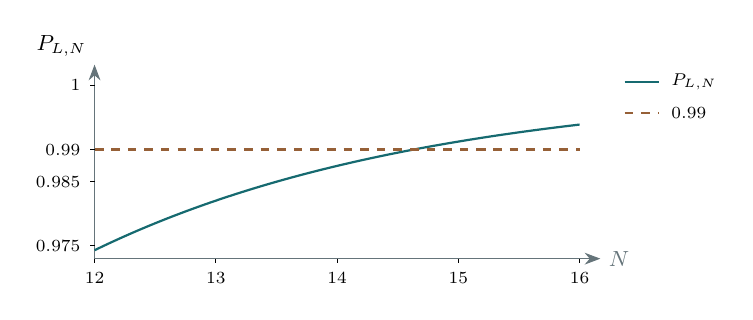
\begin{tikzpicture}[scale=.88,transform shape]
\draw[axis] (0,0)--(7.3,0) node[right] {$N$};
\draw[axis] (0,0)--(0,2.8);
\node[above left] at (0,2.8) {$P_{L,N}$};
\draw[thin] (0.000000,0)--(0.000000,-0.06);\node[below,font=\scriptsize] at (0.000000,-0.08) {$ 12 $};
\draw[thin] (1.750000,0)--(1.750000,-0.06);\node[below,font=\scriptsize] at (1.750000,-0.08) {$ 13 $};
\draw[thin] (3.500000,0)--(3.500000,-0.06);\node[below,font=\scriptsize] at (3.500000,-0.08) {$ 14 $};
\draw[thin] (5.250000,0)--(5.250000,-0.06);\node[below,font=\scriptsize] at (5.250000,-0.08) {$ 15 $};
\draw[thin] (7.000000,0)--(7.000000,-0.06);\node[below,font=\scriptsize] at (7.000000,-0.08) {$ 16 $};
\draw[thin] (0,0.185185)--(-.06,0.185185);\node[left,font=\scriptsize] at (-.08,0.185185) {$ 0.975 $};
\draw[thin] (0,1.111111)--(-.06,1.111111);\node[left,font=\scriptsize] at (-.08,1.111111) {$ 0.985 $};
\draw[thin] (0,1.574074)--(-.06,1.574074);\node[left,font=\scriptsize] at (-.08,1.574074) {$ 0.99 $};
\draw[thin] (0,2.500000)--(-.06,2.500000);\node[left,font=\scriptsize] at (-.08,2.500000) {$ 1 $};
\draw[thick,color=accent] plot coordinates {(0.0000000,0.1215371) (0.0291667,0.1356547) (0.0583333,0.1496896) (0.0875000,0.1636423) (0.1166667,0.1775132) (0.1458333,0.1913027) (0.1750000,0.2050115) (0.2041667,0.2186398) (0.2333333,0.2321882) (0.2625000,0.2456572) (0.2916667,0.2590471) (0.3208333,0.2723585) (0.3500000,0.2855917) (0.3791667,0.2987473) (0.4083333,0.3118257) (0.4375000,0.3248273) (0.4666667,0.3377525) (0.4958333,0.3506019) (0.5250000,0.3633758) (0.5541667,0.3760746) (0.5833333,0.3886989) (0.6125000,0.4012489) (0.6416667,0.4137252) (0.6708333,0.4261282) (0.7000000,0.4384583) (0.7291667,0.4507159) (0.7583333,0.4629014) (0.7875000,0.4750153) (0.8166667,0.4870579) (0.8458333,0.4990297) (0.8750000,0.5109311) (0.9041667,0.5227624) (0.9333333,0.5345241) (0.9625000,0.5462166) (0.9916667,0.5578403) (1.0208333,0.5693956) (1.0500000,0.5808828) (1.0791667,0.5923024) (1.1083333,0.6036547) (1.1375000,0.6149402) (1.1666667,0.6261592) (1.1958333,0.6373121) (1.2250000,0.6483993) (1.2541667,0.6594212) (1.2833333,0.6703781) (1.3125000,0.6812704) (1.3416667,0.6920986) (1.3708333,0.7028628) (1.4000000,0.7135637) (1.4291667,0.7242014) (1.4583333,0.7347764) (1.4875000,0.7452890) (1.5166667,0.7557396) (1.5458333,0.7661286) (1.5750000,0.7764562) (1.6041667,0.7867230) (1.6333333,0.7969291) (1.6625000,0.8070750) (1.6916667,0.8171610) (1.7208333,0.8271874) (1.7500000,0.8371547) (1.7791667,0.8470631) (1.8083333,0.8569130) (1.8375000,0.8667047) (1.8666667,0.8764386) (1.8958333,0.8861150) (1.9250000,0.8957342) (1.9541667,0.9052966) (1.9833333,0.9148025) (2.0125000,0.9242522) (2.0416667,0.9336460) (2.0708333,0.9429844) (2.1000000,0.9522675) (2.1291667,0.9614957) (2.1583333,0.9706694) (2.1875000,0.9797888) (2.2166667,0.9888543) (2.2458333,0.9978662) (2.2750000,1.0068248) (2.3041667,1.0157303) (2.3333333,1.0245832) (2.3625000,1.0333837) (2.3916667,1.0421321) (2.4208333,1.0508288) (2.4500000,1.0594740) (2.4791667,1.0680680) (2.5083333,1.0766111) (2.5375000,1.0851037) (2.5666667,1.0935460) (2.5958333,1.1019382) (2.6250000,1.1102808) (2.6541667,1.1185740) (2.6833333,1.1268181) (2.7125000,1.1350133) (2.7416667,1.1431600) (2.7708333,1.1512584) (2.8000000,1.1593088) (2.8291667,1.1673116) (2.8583333,1.1752669) (2.8875000,1.1831750) (2.9166667,1.1910363) (2.9458333,1.1988510) (2.9750000,1.2066193) (3.0041667,1.2143416) (3.0333333,1.2220182) (3.0625000,1.2296491) (3.0916667,1.2372349) (3.1208333,1.2447756) (3.1500000,1.2522717) (3.1791667,1.2597232) (3.2083333,1.2671306) (3.2375000,1.2744940) (3.2666667,1.2818137) (3.2958333,1.2890900) (3.3250000,1.2963232) (3.3541667,1.3035134) (3.3833333,1.3106609) (3.4125000,1.3177660) (3.4416667,1.3248289) (3.4708333,1.3318499) (3.5000000,1.3388292) (3.5291667,1.3457671) (3.5583333,1.3526638) (3.5875000,1.3595195) (3.6166667,1.3663345) (3.6458333,1.3731091) (3.6750000,1.3798434) (3.7041667,1.3865377) (3.7333333,1.3931922) (3.7625000,1.3998072) (3.7916667,1.4063829) (3.8208333,1.4129196) (3.8500000,1.4194174) (3.8791667,1.4258766) (3.9083333,1.4322974) (3.9375000,1.4386800) (3.9666667,1.4450247) (3.9958333,1.4513317) (4.0250000,1.4576012) (4.0541667,1.4638334) (4.0833333,1.4700286) (4.1125000,1.4761869) (4.1416667,1.4823086) (4.1708333,1.4883939) (4.2000000,1.4944431) (4.2291667,1.5004562) (4.2583333,1.5064336) (4.2875000,1.5123754) (4.3166667,1.5182819) (4.3458333,1.5241533) (4.3750000,1.5299897) (4.4041667,1.5357914) (4.4333333,1.5415586) (4.4625000,1.5472915) (4.4916667,1.5529902) (4.5208333,1.5586550) (4.5500000,1.5642862) (4.5791667,1.5698838) (4.6083333,1.5754480) (4.6375000,1.5809792) (4.6666667,1.5864774) (4.6958333,1.5919430) (4.7250000,1.5973759) (4.7541667,1.6027765) (4.7833333,1.6081450) (4.8125000,1.6134815) (4.8416667,1.6187862) (4.8708333,1.6240593) (4.9000000,1.6293011) (4.9291667,1.6345116) (4.9583333,1.6396910) (4.9875000,1.6448396) (5.0166667,1.6499576) (5.0458333,1.6550450) (5.0750000,1.6601022) (5.1041667,1.6651292) (5.1333333,1.6701263) (5.1625000,1.6750935) (5.1916667,1.6800312) (5.2208333,1.6849395) (5.2500000,1.6898185) (5.2791667,1.6946684) (5.3083333,1.6994895) (5.3375000,1.7042817) (5.3666667,1.7090455) (5.3958333,1.7137808) (5.4250000,1.7184879) (5.4541667,1.7231669) (5.4833333,1.7278181) (5.5125000,1.7324415) (5.5416667,1.7370373) (5.5708333,1.7416057) (5.6000000,1.7461469) (5.6291667,1.7506610) (5.6583333,1.7551482) (5.6875000,1.7596086) (5.7166667,1.7640424) (5.7458333,1.7684498) (5.7750000,1.7728309) (5.8041667,1.7771858) (5.8333333,1.7815148) (5.8625000,1.7858180) (5.8916667,1.7900954) (5.9208333,1.7943474) (5.9500000,1.7985739) (5.9791667,1.8027753) (6.0083333,1.8069516) (6.0375000,1.8111030) (6.0666667,1.8152295) (6.0958333,1.8193315) (6.1250000,1.8234090) (6.1541667,1.8274621) (6.1833333,1.8314911) (6.2125000,1.8354960) (6.2416667,1.8394770) (6.2708333,1.8434342) (6.3000000,1.8473678) (6.3291667,1.8512779) (6.3583333,1.8551647) (6.3875000,1.8590283) (6.4166667,1.8628688) (6.4458333,1.8666864) (6.4750000,1.8704811) (6.5041667,1.8742533) (6.5333333,1.8780028) (6.5625000,1.8817300) (6.5916667,1.8854350) (6.6208333,1.8891178) (6.6500000,1.8927786) (6.6791667,1.8964175) (6.7083333,1.9000347) (6.7375000,1.9036303) (6.7666667,1.9072045) (6.7958333,1.9107572) (6.8250000,1.9142888) (6.8541667,1.9177992) (6.8833333,1.9212887) (6.9125000,1.9247573) (6.9416667,1.9282052) (6.9708333,1.9316325) (7.0000000,1.9350393)};
\draw[thick,color=accent] (7.65,2.55)--(8.15,2.55);\node[right,font=\scriptsize] at (8.2,2.55) {$P_{L,N}$};
\draw[thick,dashed,color=warm] plot coordinates {(0.0000000,1.5740741) (0.0291667,1.5740741) (0.0583333,1.5740741) (0.0875000,1.5740741) (0.1166667,1.5740741) (0.1458333,1.5740741) (0.1750000,1.5740741) (0.2041667,1.5740741) (0.2333333,1.5740741) (0.2625000,1.5740741) (0.2916667,1.5740741) (0.3208333,1.5740741) (0.3500000,1.5740741) (0.3791667,1.5740741) (0.4083333,1.5740741) (0.4375000,1.5740741) (0.4666667,1.5740741) (0.4958333,1.5740741) (0.5250000,1.5740741) (0.5541667,1.5740741) (0.5833333,1.5740741) (0.6125000,1.5740741) (0.6416667,1.5740741) (0.6708333,1.5740741) (0.7000000,1.5740741) (0.7291667,1.5740741) (0.7583333,1.5740741) (0.7875000,1.5740741) (0.8166667,1.5740741) (0.8458333,1.5740741) (0.8750000,1.5740741) (0.9041667,1.5740741) (0.9333333,1.5740741) (0.9625000,1.5740741) (0.9916667,1.5740741) (1.0208333,1.5740741) (1.0500000,1.5740741) (1.0791667,1.5740741) (1.1083333,1.5740741) (1.1375000,1.5740741) (1.1666667,1.5740741) (1.1958333,1.5740741) (1.2250000,1.5740741) (1.2541667,1.5740741) (1.2833333,1.5740741) (1.3125000,1.5740741) (1.3416667,1.5740741) (1.3708333,1.5740741) (1.4000000,1.5740741) (1.4291667,1.5740741) (1.4583333,1.5740741) (1.4875000,1.5740741) (1.5166667,1.5740741) (1.5458333,1.5740741) (1.5750000,1.5740741) (1.6041667,1.5740741) (1.6333333,1.5740741) (1.6625000,1.5740741) (1.6916667,1.5740741) (1.7208333,1.5740741) (1.7500000,1.5740741) (1.7791667,1.5740741) (1.8083333,1.5740741) (1.8375000,1.5740741) (1.8666667,1.5740741) (1.8958333,1.5740741) (1.9250000,1.5740741) (1.9541667,1.5740741) (1.9833333,1.5740741) (2.0125000,1.5740741) (2.0416667,1.5740741) (2.0708333,1.5740741) (2.1000000,1.5740741) (2.1291667,1.5740741) (2.1583333,1.5740741) (2.1875000,1.5740741) (2.2166667,1.5740741) (2.2458333,1.5740741) (2.2750000,1.5740741) (2.3041667,1.5740741) (2.3333333,1.5740741) (2.3625000,1.5740741) (2.3916667,1.5740741) (2.4208333,1.5740741) (2.4500000,1.5740741) (2.4791667,1.5740741) (2.5083333,1.5740741) (2.5375000,1.5740741) (2.5666667,1.5740741) (2.5958333,1.5740741) (2.6250000,1.5740741) (2.6541667,1.5740741) (2.6833333,1.5740741) (2.7125000,1.5740741) (2.7416667,1.5740741) (2.7708333,1.5740741) (2.8000000,1.5740741) (2.8291667,1.5740741) (2.8583333,1.5740741) (2.8875000,1.5740741) (2.9166667,1.5740741) (2.9458333,1.5740741) (2.9750000,1.5740741) (3.0041667,1.5740741) (3.0333333,1.5740741) (3.0625000,1.5740741) (3.0916667,1.5740741) (3.1208333,1.5740741) (3.1500000,1.5740741) (3.1791667,1.5740741) (3.2083333,1.5740741) (3.2375000,1.5740741) (3.2666667,1.5740741) (3.2958333,1.5740741) (3.3250000,1.5740741) (3.3541667,1.5740741) (3.3833333,1.5740741) (3.4125000,1.5740741) (3.4416667,1.5740741) (3.4708333,1.5740741) (3.5000000,1.5740741) (3.5291667,1.5740741) (3.5583333,1.5740741) (3.5875000,1.5740741) (3.6166667,1.5740741) (3.6458333,1.5740741) (3.6750000,1.5740741) (3.7041667,1.5740741) (3.7333333,1.5740741) (3.7625000,1.5740741) (3.7916667,1.5740741) (3.8208333,1.5740741) (3.8500000,1.5740741) (3.8791667,1.5740741) (3.9083333,1.5740741) (3.9375000,1.5740741) (3.9666667,1.5740741) (3.9958333,1.5740741) (4.0250000,1.5740741) (4.0541667,1.5740741) (4.0833333,1.5740741) (4.1125000,1.5740741) (4.1416667,1.5740741) (4.1708333,1.5740741) (4.2000000,1.5740741) (4.2291667,1.5740741) (4.2583333,1.5740741) (4.2875000,1.5740741) (4.3166667,1.5740741) (4.3458333,1.5740741) (4.3750000,1.5740741) (4.4041667,1.5740741) (4.4333333,1.5740741) (4.4625000,1.5740741) (4.4916667,1.5740741) (4.5208333,1.5740741) (4.5500000,1.5740741) (4.5791667,1.5740741) (4.6083333,1.5740741) (4.6375000,1.5740741) (4.6666667,1.5740741) (4.6958333,1.5740741) (4.7250000,1.5740741) (4.7541667,1.5740741) (4.7833333,1.5740741) (4.8125000,1.5740741) (4.8416667,1.5740741) (4.8708333,1.5740741) (4.9000000,1.5740741) (4.9291667,1.5740741) (4.9583333,1.5740741) (4.9875000,1.5740741) (5.0166667,1.5740741) (5.0458333,1.5740741) (5.0750000,1.5740741) (5.1041667,1.5740741) (5.1333333,1.5740741) (5.1625000,1.5740741) (5.1916667,1.5740741) (5.2208333,1.5740741) (5.2500000,1.5740741) (5.2791667,1.5740741) (5.3083333,1.5740741) (5.3375000,1.5740741) (5.3666667,1.5740741) (5.3958333,1.5740741) (5.4250000,1.5740741) (5.4541667,1.5740741) (5.4833333,1.5740741) (5.5125000,1.5740741) (5.5416667,1.5740741) (5.5708333,1.5740741) (5.6000000,1.5740741) (5.6291667,1.5740741) (5.6583333,1.5740741) (5.6875000,1.5740741) (5.7166667,1.5740741) (5.7458333,1.5740741) (5.7750000,1.5740741) (5.8041667,1.5740741) (5.8333333,1.5740741) (5.8625000,1.5740741) (5.8916667,1.5740741) (5.9208333,1.5740741) (5.9500000,1.5740741) (5.9791667,1.5740741) (6.0083333,1.5740741) (6.0375000,1.5740741) (6.0666667,1.5740741) (6.0958333,1.5740741) (6.1250000,1.5740741) (6.1541667,1.5740741) (6.1833333,1.5740741) (6.2125000,1.5740741) (6.2416667,1.5740741) (6.2708333,1.5740741) (6.3000000,1.5740741) (6.3291667,1.5740741) (6.3583333,1.5740741) (6.3875000,1.5740741) (6.4166667,1.5740741) (6.4458333,1.5740741) (6.4750000,1.5740741) (6.5041667,1.5740741) (6.5333333,1.5740741) (6.5625000,1.5740741) (6.5916667,1.5740741) (6.6208333,1.5740741) (6.6500000,1.5740741) (6.6791667,1.5740741) (6.7083333,1.5740741) (6.7375000,1.5740741) (6.7666667,1.5740741) (6.7958333,1.5740741) (6.8250000,1.5740741) (6.8541667,1.5740741) (6.8833333,1.5740741) (6.9125000,1.5740741) (6.9416667,1.5740741) (6.9708333,1.5740741) (7.0000000,1.5740741)};
\draw[thick,dashed,color=warm] (7.65,2.0999999999999996)--(8.15,2.0999999999999996);\node[right,font=\scriptsize] at (8.2,2.0999999999999996) {$0.99$};
\end{tikzpicture}
\figcaption{解图光4.7C\quad 14片与15片分居99百分比阈值两侧}
\end{minipage}\end{center}
再把两条功率链相加，可得主透射束的总功率
\[
 P_N=\frac{P_0}{2}(1+q^{2N}),\qquad
 \frac{P_N}{P_0}=\frac{1}{1+P_{L,N}}.
\]
解图光4.7D中总功率从$P_0$单调降向$P_0/2$；$15$片时为$0.502197P_0$。增加玻璃片使$s$分量逐步反射到主束以外，$p$分量保留最初的$P_0/2$，因而高偏振度与约一半的透射功率同时出现。上述链条对应同向放置、各面布儒斯特入射并只收主透射束的片堆；反射副束也进入探测器时，各副束的路径和功率另行相加。
\begin{center}\begin{minipage}{.98\linewidth}\centering
\begin{tikzpicture}[scale=.88,transform shape]
\draw[axis] (0,0)--(7.3,0) node[right] {$N$};
\draw[axis] (0,0)--(0,2.8);
\node[above left] at (0,2.8) {$P_N/P_0$};
\draw[thin] (0.000000,0)--(0.000000,-0.06);\node[below,font=\scriptsize] at (0.000000,-0.08) {$ 0 $};
\draw[thin] (1.400000,0)--(1.400000,-0.06);\node[below,font=\scriptsize] at (1.400000,-0.08) {$ 4 $};
\draw[thin] (2.800000,0)--(2.800000,-0.06);\node[below,font=\scriptsize] at (2.800000,-0.08) {$ 8 $};
\draw[thin] (4.200000,0)--(4.200000,-0.06);\node[below,font=\scriptsize] at (4.200000,-0.08) {$ 12 $};
\draw[thin] (5.600000,0)--(5.600000,-0.06);\node[below,font=\scriptsize] at (5.600000,-0.08) {$ 16 $};
\draw[thin] (7.000000,0)--(7.000000,-0.06);\node[below,font=\scriptsize] at (7.000000,-0.08) {$ 20 $};
\draw[thin] (0,0.047170)--(-.06,0.047170);\node[left,font=\scriptsize] at (-.08,0.047170) {$ 0.5 $};
\draw[thin] (0,1.226415)--(-.06,1.226415);\node[left,font=\scriptsize] at (-.08,1.226415) {$ 0.75 $};
\draw[thin] (0,2.405660)--(-.06,2.405660);\node[left,font=\scriptsize] at (-.08,2.405660) {$ 1 $};
\draw[thick,color=accent] plot coordinates {(0.0000000,2.4056604) (0.0291667,2.3356072) (0.0583333,2.2676348) (0.0875000,2.2016813) (0.1166667,2.1376868) (0.1458333,2.0755931) (0.1750000,2.0153438) (0.2041667,1.9568840) (0.2333333,1.9001606) (0.2625000,1.8451221) (0.2916667,1.7917183) (0.3208333,1.7399008) (0.3500000,1.6896223) (0.3791667,1.6408373) (0.4083333,1.5935013) (0.4375000,1.5475713) (0.4666667,1.5030056) (0.4958333,1.4597636) (0.5250000,1.4178059) (0.5541667,1.3770945) (0.5833333,1.3375924) (0.6125000,1.2992635) (0.6416667,1.2620732) (0.6708333,1.2259874) (0.7000000,1.1909736) (0.7291667,1.1569997) (0.7583333,1.1240349) (0.7875000,1.0920493) (0.8166667,1.0610137) (0.8458333,1.0308999) (0.8750000,1.0016806) (0.9041667,0.9733292) (0.9333333,0.9458199) (0.9625000,0.9191277) (0.9916667,0.8932284) (1.0208333,0.8680983) (1.0500000,0.8437146) (1.0791667,0.8200552) (1.1083333,0.7970985) (1.1375000,0.7748237) (1.1666667,0.7532106) (1.1958333,0.7322393) (1.2250000,0.7118910) (1.2541667,0.6921471) (1.2833333,0.6729896) (1.3125000,0.6544012) (1.3416667,0.6363649) (1.3708333,0.6188643) (1.4000000,0.6018835) (1.4291667,0.5854071) (1.4583333,0.5694201) (1.4875000,0.5539079) (1.5166667,0.5388565) (1.5458333,0.5242521) (1.5750000,0.5100816) (1.6041667,0.4963319) (1.6333333,0.4829907) (1.6625000,0.4700457) (1.6916667,0.4574852) (1.7208333,0.4452978) (1.7500000,0.4334724) (1.7791667,0.4219982) (1.8083333,0.4108648) (1.8375000,0.4000622) (1.8666667,0.3895804) (1.8958333,0.3794099) (1.9250000,0.3695415) (1.9541667,0.3599663) (1.9833333,0.3506754) (2.0125000,0.3416605) (2.0416667,0.3329134) (2.0708333,0.3244261) (2.1000000,0.3161909) (2.1291667,0.3082002) (2.1583333,0.3004470) (2.1875000,0.2929240) (2.2166667,0.2856245) (2.2458333,0.2785418) (2.2750000,0.2716694) (2.3041667,0.2650012) (2.3333333,0.2585311) (2.3625000,0.2522531) (2.3916667,0.2461616) (2.4208333,0.2402510) (2.4500000,0.2345160) (2.4791667,0.2289514) (2.5083333,0.2235520) (2.5375000,0.2183130) (2.5666667,0.2132296) (2.5958333,0.2082972) (2.6250000,0.2035113) (2.6541667,0.1988676) (2.6833333,0.1943618) (2.7125000,0.1899898) (2.7416667,0.1857477) (2.7708333,0.1816316) (2.8000000,0.1776377) (2.8291667,0.1737625) (2.8583333,0.1700023) (2.8875000,0.1663539) (2.9166667,0.1628138) (2.9458333,0.1593789) (2.9750000,0.1560460) (3.0041667,0.1528121) (3.0333333,0.1496743) (3.0625000,0.1466296) (3.0916667,0.1436754) (3.1208333,0.1408090) (3.1500000,0.1380276) (3.1791667,0.1353289) (3.2083333,0.1327104) (3.2375000,0.1301696) (3.2666667,0.1277043) (3.2958333,0.1253122) (3.3250000,0.1229912) (3.3541667,0.1207391) (3.3833333,0.1185539) (3.4125000,0.1164336) (3.4416667,0.1143763) (3.4708333,0.1123801) (3.5000000,0.1104432) (3.5291667,0.1085638) (3.5583333,0.1067402) (3.5875000,0.1049709) (3.6166667,0.1032540) (3.6458333,0.1015882) (3.6750000,0.0999718) (3.7041667,0.0984035) (3.7333333,0.0968817) (3.7625000,0.0954051) (3.7916667,0.0939724) (3.8208333,0.0925822) (3.8500000,0.0912334) (3.8791667,0.0899246) (3.9083333,0.0886547) (3.9375000,0.0874224) (3.9666667,0.0862268) (3.9958333,0.0850668) (4.0250000,0.0839411) (4.0541667,0.0828489) (4.0833333,0.0817892) (4.1125000,0.0807609) (4.1416667,0.0797631) (4.1708333,0.0787950) (4.2000000,0.0778557) (4.2291667,0.0769442) (4.2583333,0.0760599) (4.2875000,0.0752017) (4.3166667,0.0743691) (4.3458333,0.0735612) (4.3750000,0.0727773) (4.4041667,0.0720167) (4.4333333,0.0712787) (4.4625000,0.0705626) (4.4916667,0.0698678) (4.5208333,0.0691936) (4.5500000,0.0685394) (4.5791667,0.0679047) (4.6083333,0.0672888) (4.6375000,0.0666912) (4.6666667,0.0661114) (4.6958333,0.0655488) (4.7250000,0.0650029) (4.7541667,0.0644732) (4.7833333,0.0639592) (4.8125000,0.0634606) (4.8416667,0.0629767) (4.8708333,0.0625072) (4.9000000,0.0620516) (4.9291667,0.0616096) (4.9583333,0.0611807) (4.9875000,0.0607645) (5.0166667,0.0603607) (5.0458333,0.0599689) (5.0750000,0.0595888) (5.1041667,0.0592199) (5.1333333,0.0588620) (5.1625000,0.0585147) (5.1916667,0.0581777) (5.2208333,0.0578508) (5.2500000,0.0575335) (5.2791667,0.0572257) (5.3083333,0.0569270) (5.3375000,0.0566372) (5.3666667,0.0563560) (5.3958333,0.0560831) (5.4250000,0.0558184) (5.4541667,0.0555615) (5.4833333,0.0553122) (5.5125000,0.0550704) (5.5416667,0.0548357) (5.5708333,0.0546080) (5.6000000,0.0543871) (5.6291667,0.0541727) (5.6583333,0.0539647) (5.6875000,0.0537629) (5.7166667,0.0535671) (5.7458333,0.0533770) (5.7750000,0.0531927) (5.8041667,0.0530138) (5.8333333,0.0528402) (5.8625000,0.0526718) (5.8916667,0.0525083) (5.9208333,0.0523498) (5.9500000,0.0521959) (5.9791667,0.0520466) (6.0083333,0.0519018) (6.0375000,0.0517612) (6.0666667,0.0516248) (6.0958333,0.0514925) (6.1250000,0.0513641) (6.1541667,0.0512395) (6.1833333,0.0511187) (6.2125000,0.0510014) (6.2416667,0.0508876) (6.2708333,0.0507771) (6.3000000,0.0506700) (6.3291667,0.0505660) (6.3583333,0.0504652) (6.3875000,0.0503673) (6.4166667,0.0502723) (6.4458333,0.0501801) (6.4750000,0.0500907) (6.5041667,0.0500040) (6.5333333,0.0499198) (6.5625000,0.0498381) (6.5916667,0.0497589) (6.6208333,0.0496820) (6.6500000,0.0496073) (6.6791667,0.0495349) (6.7083333,0.0494647) (6.7375000,0.0493965) (6.7666667,0.0493304) (6.7958333,0.0492662) (6.8250000,0.0492039) (6.8541667,0.0491435) (6.8833333,0.0490849) (6.9125000,0.0490280) (6.9416667,0.0489728) (6.9708333,0.0489193) (7.0000000,0.0488673)};
\draw[thick,color=accent] (7.65,2.55)--(8.15,2.55);\node[right,font=\scriptsize] at (8.2,2.55) {$P_N/P_0$};
\draw[thick,dashed,color=warm] plot coordinates {(0.0000000,0.0471698) (0.0291667,0.0471698) (0.0583333,0.0471698) (0.0875000,0.0471698) (0.1166667,0.0471698) (0.1458333,0.0471698) (0.1750000,0.0471698) (0.2041667,0.0471698) (0.2333333,0.0471698) (0.2625000,0.0471698) (0.2916667,0.0471698) (0.3208333,0.0471698) (0.3500000,0.0471698) (0.3791667,0.0471698) (0.4083333,0.0471698) (0.4375000,0.0471698) (0.4666667,0.0471698) (0.4958333,0.0471698) (0.5250000,0.0471698) (0.5541667,0.0471698) (0.5833333,0.0471698) (0.6125000,0.0471698) (0.6416667,0.0471698) (0.6708333,0.0471698) (0.7000000,0.0471698) (0.7291667,0.0471698) (0.7583333,0.0471698) (0.7875000,0.0471698) (0.8166667,0.0471698) (0.8458333,0.0471698) (0.8750000,0.0471698) (0.9041667,0.0471698) (0.9333333,0.0471698) (0.9625000,0.0471698) (0.9916667,0.0471698) (1.0208333,0.0471698) (1.0500000,0.0471698) (1.0791667,0.0471698) (1.1083333,0.0471698) (1.1375000,0.0471698) (1.1666667,0.0471698) (1.1958333,0.0471698) (1.2250000,0.0471698) (1.2541667,0.0471698) (1.2833333,0.0471698) (1.3125000,0.0471698) (1.3416667,0.0471698) (1.3708333,0.0471698) (1.4000000,0.0471698) (1.4291667,0.0471698) (1.4583333,0.0471698) (1.4875000,0.0471698) (1.5166667,0.0471698) (1.5458333,0.0471698) (1.5750000,0.0471698) (1.6041667,0.0471698) (1.6333333,0.0471698) (1.6625000,0.0471698) (1.6916667,0.0471698) (1.7208333,0.0471698) (1.7500000,0.0471698) (1.7791667,0.0471698) (1.8083333,0.0471698) (1.8375000,0.0471698) (1.8666667,0.0471698) (1.8958333,0.0471698) (1.9250000,0.0471698) (1.9541667,0.0471698) (1.9833333,0.0471698) (2.0125000,0.0471698) (2.0416667,0.0471698) (2.0708333,0.0471698) (2.1000000,0.0471698) (2.1291667,0.0471698) (2.1583333,0.0471698) (2.1875000,0.0471698) (2.2166667,0.0471698) (2.2458333,0.0471698) (2.2750000,0.0471698) (2.3041667,0.0471698) (2.3333333,0.0471698) (2.3625000,0.0471698) (2.3916667,0.0471698) (2.4208333,0.0471698) (2.4500000,0.0471698) (2.4791667,0.0471698) (2.5083333,0.0471698) (2.5375000,0.0471698) (2.5666667,0.0471698) (2.5958333,0.0471698) (2.6250000,0.0471698) (2.6541667,0.0471698) (2.6833333,0.0471698) (2.7125000,0.0471698) (2.7416667,0.0471698) (2.7708333,0.0471698) (2.8000000,0.0471698) (2.8291667,0.0471698) (2.8583333,0.0471698) (2.8875000,0.0471698) (2.9166667,0.0471698) (2.9458333,0.0471698) (2.9750000,0.0471698) (3.0041667,0.0471698) (3.0333333,0.0471698) (3.0625000,0.0471698) (3.0916667,0.0471698) (3.1208333,0.0471698) (3.1500000,0.0471698) (3.1791667,0.0471698) (3.2083333,0.0471698) (3.2375000,0.0471698) (3.2666667,0.0471698) (3.2958333,0.0471698) (3.3250000,0.0471698) (3.3541667,0.0471698) (3.3833333,0.0471698) (3.4125000,0.0471698) (3.4416667,0.0471698) (3.4708333,0.0471698) (3.5000000,0.0471698) (3.5291667,0.0471698) (3.5583333,0.0471698) (3.5875000,0.0471698) (3.6166667,0.0471698) (3.6458333,0.0471698) (3.6750000,0.0471698) (3.7041667,0.0471698) (3.7333333,0.0471698) (3.7625000,0.0471698) (3.7916667,0.0471698) (3.8208333,0.0471698) (3.8500000,0.0471698) (3.8791667,0.0471698) (3.9083333,0.0471698) (3.9375000,0.0471698) (3.9666667,0.0471698) (3.9958333,0.0471698) (4.0250000,0.0471698) (4.0541667,0.0471698) (4.0833333,0.0471698) (4.1125000,0.0471698) (4.1416667,0.0471698) (4.1708333,0.0471698) (4.2000000,0.0471698) (4.2291667,0.0471698) (4.2583333,0.0471698) (4.2875000,0.0471698) (4.3166667,0.0471698) (4.3458333,0.0471698) (4.3750000,0.0471698) (4.4041667,0.0471698) (4.4333333,0.0471698) (4.4625000,0.0471698) (4.4916667,0.0471698) (4.5208333,0.0471698) (4.5500000,0.0471698) (4.5791667,0.0471698) (4.6083333,0.0471698) (4.6375000,0.0471698) (4.6666667,0.0471698) (4.6958333,0.0471698) (4.7250000,0.0471698) (4.7541667,0.0471698) (4.7833333,0.0471698) (4.8125000,0.0471698) (4.8416667,0.0471698) (4.8708333,0.0471698) (4.9000000,0.0471698) (4.9291667,0.0471698) (4.9583333,0.0471698) (4.9875000,0.0471698) (5.0166667,0.0471698) (5.0458333,0.0471698) (5.0750000,0.0471698) (5.1041667,0.0471698) (5.1333333,0.0471698) (5.1625000,0.0471698) (5.1916667,0.0471698) (5.2208333,0.0471698) (5.2500000,0.0471698) (5.2791667,0.0471698) (5.3083333,0.0471698) (5.3375000,0.0471698) (5.3666667,0.0471698) (5.3958333,0.0471698) (5.4250000,0.0471698) (5.4541667,0.0471698) (5.4833333,0.0471698) (5.5125000,0.0471698) (5.5416667,0.0471698) (5.5708333,0.0471698) (5.6000000,0.0471698) (5.6291667,0.0471698) (5.6583333,0.0471698) (5.6875000,0.0471698) (5.7166667,0.0471698) (5.7458333,0.0471698) (5.7750000,0.0471698) (5.8041667,0.0471698) (5.8333333,0.0471698) (5.8625000,0.0471698) (5.8916667,0.0471698) (5.9208333,0.0471698) (5.9500000,0.0471698) (5.9791667,0.0471698) (6.0083333,0.0471698) (6.0375000,0.0471698) (6.0666667,0.0471698) (6.0958333,0.0471698) (6.1250000,0.0471698) (6.1541667,0.0471698) (6.1833333,0.0471698) (6.2125000,0.0471698) (6.2416667,0.0471698) (6.2708333,0.0471698) (6.3000000,0.0471698) (6.3291667,0.0471698) (6.3583333,0.0471698) (6.3875000,0.0471698) (6.4166667,0.0471698) (6.4458333,0.0471698) (6.4750000,0.0471698) (6.5041667,0.0471698) (6.5333333,0.0471698) (6.5625000,0.0471698) (6.5916667,0.0471698) (6.6208333,0.0471698) (6.6500000,0.0471698) (6.6791667,0.0471698) (6.7083333,0.0471698) (6.7375000,0.0471698) (6.7666667,0.0471698) (6.7958333,0.0471698) (6.8250000,0.0471698) (6.8541667,0.0471698) (6.8833333,0.0471698) (6.9125000,0.0471698) (6.9416667,0.0471698) (6.9708333,0.0471698) (7.0000000,0.0471698)};
\draw[thick,dashed,color=warm] (7.65,2.0999999999999996)--(8.15,2.0999999999999996);\node[right,font=\scriptsize] at (8.2,2.0999999999999996) {$1/2$};
\end{tikzpicture}
\figcaption{解图光4.7D\quad 主束总功率趋向输入功率的一半}
\end{minipage}\end{center}


\Needspace{13\baselineskip}

\pdfbookmark[2]{第 8 题 全反射引入的相位差}{q8}

\section*{第 8 题\quad 全反射引入的相位差}\label{q:8}

线偏振光从折射率$n_1$的透明介质射向$n_2<n_1$的透明介质，入射角超过临界角。证明反射光一般为椭圆偏振，求两偏振分量的相对相位差，并说明仍保持线偏振的例外。

\begin{center}\begin{minipage}{.98\linewidth}\centering
\begin{tikzpicture}[scale=.9,transform shape]
\draw[object] (-3.10000,0.00000)--(3.50000,0.00000);\draw[guide] (0.00000,-2.50000)--(0.00000,2.70000);\fill (0.00000,0.00000) circle(.035);\node[above right] at (0.00000,0.00000) {$O$};\draw[motion] (-1.91511,1.60697)--(0.00000,0.00000);
\draw[motion] (0.00000,0.00000)--(1.91511,1.60697);\draw[thin,color=accent] (-2.70000,-0.10000)--(-2.70000,-0.60000);\draw[thin,color=accent] (-2.34000,-0.10000)--(-2.34000,-0.60000);\draw[thin,color=accent] (-1.98000,-0.10000)--(-1.98000,-0.60000);\draw[thin,color=accent] (-1.62000,-0.10000)--(-1.62000,-0.60000);\draw[thin,color=accent] (-1.26000,-0.10000)--(-1.26000,-0.60000);\draw[thin,color=accent] (-0.90000,-0.10000)--(-0.90000,-0.60000);\draw[thin,color=accent] (-0.54000,-0.10000)--(-0.54000,-0.60000);\draw[thin,color=accent] (-0.18000,-0.10000)--(-0.18000,-0.60000);\draw[thin,color=accent] (0.18000,-0.10000)--(0.18000,-0.60000);\draw[thin,color=accent] (0.54000,-0.10000)--(0.54000,-0.60000);\draw[thin,color=accent] (0.90000,-0.10000)--(0.90000,-0.60000);\draw[thin,color=accent] (1.26000,-0.10000)--(1.26000,-0.60000);\draw[thin,color=accent] (1.62000,-0.10000)--(1.62000,-0.60000);\draw[thin,color=accent] (1.98000,-0.10000)--(1.98000,-0.60000);\draw[thin,color=accent] (2.34000,-0.10000)--(2.34000,-0.60000);\draw[thin,color=accent] (2.70000,-0.10000)--(2.70000,-0.60000);\node[below] at (2.10000,-1.50000) {倏逝场};\node[right] at (-2.90000,1.50000) {$n_1$};\node[right] at (-2.90000,-1.50000) {$n_2$};\node[left] at (-0.50000,1.00000) {$\theta_i$};\node[right] at (0.55000,1.10000) {$\theta_r$};
\end{tikzpicture}
\figcaption{图光4.8\quad 全反射与第二介质中的倏逝场}
\end{minipage}\end{center}

\Needspace{6\baselineskip}\subsection*{解答}


在图光4.8中取法向坐标$z$从界面$O$指向第二介质，故介质2位于$z>0$。两介质均透明、非磁，$0<m=n_2/n_1<1$，入射角满足$\theta_c=\arcsin m<\theta<\pi/2$。每束光取有向基矢$\boldsymbol p=\boldsymbol s\times\hat{\boldsymbol k}$，场的时间因子为$e^{-i\omega t}$。切向波矢连续给出
\[
 n_2^2\cos^2\theta_t=n_2^2-n_1^2\sin^2\theta
 =-n_1^2g^2,\qquad g=\sqrt{\sin^2\theta-m^2}>0.
\]
选择$n_2\cos\theta_t=i n_1g$，第二介质场含$e^{-k_0n_1gz}$，从$O$向内衰减；图中下方的倏逝场正对应这一根。令$c_\theta=\cos\theta$，将该根代入菲涅耳式，得
\[
r_s=\frac{c_\theta-ig}{c_\theta+ig}=e^{-2i\phi_s},\quad
r_p=\frac{m^2c_\theta-ig}{m^2c_\theta+ig}=e^{-2i\phi_p},
\]
其中两复分数的分子、分母互为共轭，模均为1。把分母写成模乘相位，便有
\[
\phi_s=\arctan\frac g{c_\theta},\qquad
\phi_p=\arctan\frac g{m^2c_\theta}.
\]
于是$r_s$、$r_p$的辐角分别为$-2\phi_s$、$-2\phi_p$。解图光4.8A左侧画出两个反射系数，右侧画出等幅分量的电场轨迹。图例取$n_1/n_2=1.5$、$\theta=50.22945^\circ$，此时两反射系数相隔$45^\circ$；左右面板按各自变量归一化。
\begin{center}\begin{minipage}{.98\linewidth}\centering
\begin{tikzpicture}[scale=.8,transform shape]
\draw[object] (0.00000,0.00000) circle(1.50000);\draw[axis] (-1.60000,0.00000)--(1.60000,0.00000);\draw[axis] (0.00000,-1.60000)--(0.00000,1.60000);\node[below right] at (1.60000,0.00000) {$\operatorname{Re}r$};\node[above right] at (0.00000,1.60000) {$\operatorname{Im}r$};\draw[motion] (0.00000,0.00000)--(0.70987,-1.32140);\draw[force] (0.00000,0.00000)--(-0.43241,-1.43632);\node[right] at (0.85184,-1.58567) {$r_s$};\node[below] at (-0.51890,-1.72358) {$r_p$};\node[above] at (0.00000,2.00000) {单位模，不同相位};\begin{scope}[shift={(5.00000,0.00000)}]
\draw[axis] (-1.50000,0.00000)--(1.50000,0.00000);\draw[axis] (0.00000,-1.50000)--(0.00000,1.50000);\node[below right] at (1.50000,0.00000) {$E_p/a$};\node[above right] at (0.00000,1.50000) {$E_s/b$};\draw[traj] plot coordinates {(1.06066,0.75000) (1.06001,0.77572) (1.05808,0.80049) (1.05485,0.82429) (1.05034,0.84708) (1.04455,0.86884) (1.03748,0.88954) (1.02915,0.90916) (1.01957,0.92767) (1.00875,0.94506) (0.99669,0.96128) (0.98343,0.97634) (0.96896,0.99021) (0.95332,1.00287) (0.93651,1.01431) (0.91856,1.02452) (0.89949,1.03348) (0.87933,1.04117) (0.85809,1.04760) (0.83581,1.05275) (0.81251,1.05662) (0.78822,1.05921) (0.76298,1.06050) (0.73680,1.06050) (0.70972,1.05921) (0.68178,1.05662) (0.65301,1.05275) (0.62344,1.04760) (0.59311,1.04117) (0.56206,1.03348) (0.53033,1.02452) (0.49795,1.01431) (0.46496,1.00287) (0.43141,0.99021) (0.39733,0.97634) (0.36277,0.96128) (0.32776,0.94506) (0.29236,0.92767) (0.25660,0.90916) (0.22052,0.88954) (0.18418,0.86884) (0.14762,0.84708) (0.11087,0.82429) (0.07399,0.80049) (0.03702,0.77572) (0.00000,0.75000) (-0.03702,0.72337) (-0.07399,0.69586) (-0.11087,0.66750) (-0.14762,0.63832) (-0.18418,0.60837) (-0.22052,0.57768) (-0.25660,0.54628) (-0.29236,0.51422) (-0.32776,0.48153) (-0.36277,0.44825) (-0.39733,0.41443) (-0.43141,0.38011) (-0.46496,0.34532) (-0.49795,0.31011) (-0.53033,0.27452) (-0.56206,0.23860) (-0.59311,0.20238) (-0.62344,0.16592) (-0.65301,0.12926) (-0.68178,0.09244) (-0.70972,0.05551) (-0.73680,0.01851) (-0.76298,-0.01851) (-0.78822,-0.05551) (-0.81251,-0.09244) (-0.83581,-0.12926) (-0.85809,-0.16592) (-0.87933,-0.20238) (-0.89949,-0.23860) (-0.91856,-0.27452) (-0.93651,-0.31011) (-0.95332,-0.34532) (-0.96896,-0.38011) (-0.98343,-0.41443) (-0.99669,-0.44825) (-1.00875,-0.48153) (-1.01957,-0.51422) (-1.02915,-0.54628) (-1.03748,-0.57768) (-1.04455,-0.60837) (-1.05034,-0.63832) (-1.05485,-0.66750) (-1.05808,-0.69586) (-1.06001,-0.72337) (-1.06066,-0.75000) (-1.06001,-0.77572) (-1.05808,-0.80049) (-1.05485,-0.82429) (-1.05034,-0.84708) (-1.04455,-0.86884) (-1.03748,-0.88954) (-1.02915,-0.90916) (-1.01957,-0.92767) (-1.00875,-0.94506) (-0.99669,-0.96128) (-0.98343,-0.97634) (-0.96896,-0.99021) (-0.95332,-1.00287) (-0.93651,-1.01431) (-0.91856,-1.02452) (-0.89949,-1.03348) (-0.87933,-1.04117) (-0.85809,-1.04760) (-0.83581,-1.05275) (-0.81251,-1.05662) (-0.78822,-1.05921) (-0.76298,-1.06050) (-0.73680,-1.06050) (-0.70972,-1.05921) (-0.68178,-1.05662) (-0.65301,-1.05275) (-0.62344,-1.04760) (-0.59311,-1.04117) (-0.56206,-1.03348) (-0.53033,-1.02452) (-0.49795,-1.01431) (-0.46496,-1.00287) (-0.43141,-0.99021) (-0.39733,-0.97634) (-0.36277,-0.96128) (-0.32776,-0.94506) (-0.29236,-0.92767) (-0.25660,-0.90916) (-0.22052,-0.88954) (-0.18418,-0.86884) (-0.14762,-0.84708) (-0.11087,-0.82429) (-0.07399,-0.80049) (-0.03702,-0.77572) (-0.00000,-0.75000) (0.03702,-0.72337) (0.07399,-0.69586) (0.11087,-0.66750) (0.14762,-0.63832) (0.18418,-0.60837) (0.22052,-0.57768) (0.25660,-0.54628) (0.29236,-0.51422) (0.32776,-0.48153) (0.36277,-0.44825) (0.39733,-0.41443) (0.43141,-0.38011) (0.46496,-0.34532) (0.49795,-0.31011) (0.53033,-0.27452) (0.56206,-0.23860) (0.59311,-0.20238) (0.62344,-0.16592) (0.65301,-0.12926) (0.68178,-0.09244) (0.70972,-0.05551) (0.73680,-0.01851) (0.76298,0.01851) (0.78822,0.05551) (0.81251,0.09244) (0.83581,0.12926) (0.85809,0.16592) (0.87933,0.20238) (0.89949,0.23860) (0.91856,0.27452) (0.93651,0.31011) (0.95332,0.34532) (0.96896,0.38011) (0.98343,0.41443) (0.99669,0.44825) (1.00875,0.48153) (1.01957,0.51422) (1.02915,0.54628) (1.03748,0.57768) (1.04455,0.60837) (1.05034,0.63832) (1.05485,0.66750) (1.05808,0.69586) (1.06001,0.72337) (1.06066,0.75000)};\draw[traj,-{Stealth}] (0.53033,1.02452)--(0.39733,0.97634);\node[above] at (0.00000,2.05000) {两非零分量形成椭圆};
\end{scope}
\end{tikzpicture}
\figcaption{解图光4.8A\quad 反射系数单位圆及反射电场轨迹}
\end{minipage}\end{center}
以$p$相位为公共参考，$s$相对$p$的相位为
\[
\delta=\arg r_s-\arg r_p=2(\phi_p-\phi_s),\qquad
\tan\frac\delta2
=\frac{g c_\theta}{\sin^2\theta}.
\]
从正切差式逐项化简可看出该结果的符号和范围：
\[
 \tan(\phi_p-\phi_s)
 =\frac{g/(m^2c_\theta)-g/c_\theta}{1+g^2/(m^2c_\theta^2)}
 =\frac{gc_\theta(1-m^2)}{m^2c_\theta^2+g^2},\qquad
 m^2c_\theta^2+g^2=(1-m^2)\sin^2\theta.
\]
严格全反射角区间内$c_\theta,g>0$，且$\phi_p>\phi_s$，所以$0<\delta<\pi$。解图光4.8B把玻璃到空气的两分量相位及相位差画成角度函数；临界角与掠入射两端均有$\delta\to0$，中间有一个最大值。
\begin{center}\begin{minipage}{.98\linewidth}\centering
\begin{tikzpicture}[scale=.88,transform shape]
\draw[axis] (0,1.875)--(7.3,1.875) node[right] {$\theta/{}^\circ$};
\draw[axis] (0,0)--(0,2.8);
\node[above left] at (0,2.8) {$\text{相位}/{}^\circ$};
\draw[thin] (0.027511,1.875)--(0.027511,1.815);\node[below,font=\scriptsize] at (0.027511,1.795) {$ 42 $};
\draw[thin] (1.192019,1.875)--(1.192019,1.815);\node[below,font=\scriptsize] at (1.192019,1.795) {$ 50 $};
\draw[thin] (2.647653,1.875)--(2.647653,1.815);\node[below,font=\scriptsize] at (2.647653,1.795) {$ 60 $};
\draw[thin] (4.831105,1.875)--(4.831105,1.815);\node[below,font=\scriptsize] at (4.831105,1.795) {$ 75 $};
\draw[thin] (6.868993,1.875)--(6.868993,1.815);\node[below,font=\scriptsize] at (6.868993,1.795) {$ 89 $};
\draw[thin] (0,0.000000)--(-.06,0.000000);\node[left,font=\scriptsize] at (-.08,0.000000) {$ -180 $};
\draw[thin] (0,0.937500)--(-.06,0.937500);\node[left,font=\scriptsize] at (-.08,0.937500) {$ -90 $};
\draw[thin] (0,1.875000)--(-.06,1.875000);\node[left,font=\scriptsize] at (-.08,1.875000) {$ 0 $};
\draw[thin] (0,2.343750)--(-.06,2.343750);\node[left,font=\scriptsize] at (-.08,2.343750) {$ 45 $};
\draw[thick,color=accent] plot coordinates {(0.0000000,1.8694794) (0.0291667,1.7803098) (0.0583333,1.7410367) (0.0875000,1.7107737) (0.1166667,1.6851616) (0.1458333,1.6625119) (0.1750000,1.6419592) (0.2041667,1.6229898) (0.2333333,1.6052695) (0.2625000,1.5885662) (0.2916667,1.5727113) (0.3208333,1.5575776) (0.3500000,1.5430664) (0.3791667,1.5290993) (0.4083333,1.5156129) (0.4375000,1.5025548) (0.4666667,1.4898815) (0.4958333,1.4775561) (0.5250000,1.4655472) (0.5541667,1.4538277) (0.5833333,1.4423739) (0.6125000,1.4311654) (0.6416667,1.4201840) (0.6708333,1.4094135) (0.7000000,1.3988396) (0.7291667,1.3884495) (0.7583333,1.3782316) (0.7875000,1.3681754) (0.8166667,1.3582716) (0.8458333,1.3485114) (0.8750000,1.3388870) (0.9041667,1.3293911) (0.9333333,1.3200173) (0.9625000,1.3107593) (0.9916667,1.3016115) (1.0208333,1.2925686) (1.0500000,1.2836260) (1.0791667,1.2747790) (1.1083333,1.2660234) (1.1375000,1.2573554) (1.1666667,1.2487712) (1.1958333,1.2402675) (1.2250000,1.2318411) (1.2541667,1.2234888) (1.2833333,1.2152080) (1.3125000,1.2069958) (1.3416667,1.1988498) (1.3708333,1.1907675) (1.4000000,1.1827468) (1.4291667,1.1747855) (1.4583333,1.1668815) (1.4875000,1.1590329) (1.5166667,1.1512380) (1.5458333,1.1434949) (1.5750000,1.1358020) (1.6041667,1.1281578) (1.6333333,1.1205607) (1.6625000,1.1130093) (1.6916667,1.1055022) (1.7208333,1.0980382) (1.7500000,1.0906159) (1.7791667,1.0832342) (1.8083333,1.0758919) (1.8375000,1.0685880) (1.8666667,1.0613213) (1.8958333,1.0540909) (1.9250000,1.0468957) (1.9541667,1.0397349) (1.9833333,1.0326076) (2.0125000,1.0255128) (2.0416667,1.0184498) (2.0708333,1.0114178) (2.1000000,1.0044159) (2.1291667,0.9974434) (2.1583333,0.9904997) (2.1875000,0.9835840) (2.2166667,0.9766956) (2.2458333,0.9698339) (2.2750000,0.9629983) (2.3041667,0.9561881) (2.3333333,0.9494029) (2.3625000,0.9426419) (2.3916667,0.9359047) (2.4208333,0.9291908) (2.4500000,0.9224995) (2.4791667,0.9158305) (2.5083333,0.9091832) (2.5375000,0.9025572) (2.5666667,0.8959520) (2.5958333,0.8893672) (2.6250000,0.8828023) (2.6541667,0.8762570) (2.6833333,0.8697307) (2.7125000,0.8632232) (2.7416667,0.8567340) (2.7708333,0.8502628) (2.8000000,0.8438092) (2.8291667,0.8373729) (2.8583333,0.8309534) (2.8875000,0.8245506) (2.9166667,0.8181640) (2.9458333,0.8117933) (2.9750000,0.8054383) (3.0041667,0.7990985) (3.0333333,0.7927738) (3.0625000,0.7864639) (3.0916667,0.7801684) (3.1208333,0.7738871) (3.1500000,0.7676198) (3.1791667,0.7613661) (3.2083333,0.7551258) (3.2375000,0.7488986) (3.2666667,0.7426844) (3.2958333,0.7364829) (3.3250000,0.7302939) (3.3541667,0.7241170) (3.3833333,0.7179522) (3.4125000,0.7117992) (3.4416667,0.7056577) (3.4708333,0.6995276) (3.5000000,0.6934087) (3.5291667,0.6873008) (3.5583333,0.6812036) (3.5875000,0.6751170) (3.6166667,0.6690408) (3.6458333,0.6629749) (3.6750000,0.6569189) (3.7041667,0.6508729) (3.7333333,0.6448365) (3.7625000,0.6388097) (3.7916667,0.6327922) (3.8208333,0.6267839) (3.8500000,0.6207846) (3.8791667,0.6147943) (3.9083333,0.6088126) (3.9375000,0.6028396) (3.9666667,0.5968749) (3.9958333,0.5909186) (4.0250000,0.5849704) (4.0541667,0.5790302) (4.0833333,0.5730978) (4.1125000,0.5671732) (4.1416667,0.5612562) (4.1708333,0.5553467) (4.2000000,0.5494445) (4.2291667,0.5435495) (4.2583333,0.5376616) (4.2875000,0.5317807) (4.3166667,0.5259066) (4.3458333,0.5200392) (4.3750000,0.5141785) (4.4041667,0.5083243) (4.4333333,0.5024764) (4.4625000,0.4966349) (4.4916667,0.4907995) (4.5208333,0.4849701) (4.5500000,0.4791468) (4.5791667,0.4733292) (4.6083333,0.4675174) (4.6375000,0.4617113) (4.6666667,0.4559107) (4.6958333,0.4501156) (4.7250000,0.4443258) (4.7541667,0.4385412) (4.7833333,0.4327618) (4.8125000,0.4269875) (4.8416667,0.4212182) (4.8708333,0.4154537) (4.9000000,0.4096941) (4.9291667,0.4039391) (4.9583333,0.3981888) (4.9875000,0.3924430) (5.0166667,0.3867017) (5.0458333,0.3809647) (5.0750000,0.3752320) (5.1041667,0.3695035) (5.1333333,0.3637791) (5.1625000,0.3580587) (5.1916667,0.3523423) (5.2208333,0.3466298) (5.2500000,0.3409211) (5.2791667,0.3352161) (5.3083333,0.3295148) (5.3375000,0.3238170) (5.3666667,0.3181228) (5.3958333,0.3124319) (5.4250000,0.3067444) (5.4541667,0.3010602) (5.4833333,0.2953792) (5.5125000,0.2897014) (5.5416667,0.2840266) (5.5708333,0.2783548) (5.6000000,0.2726860) (5.6291667,0.2670200) (5.6583333,0.2613568) (5.6875000,0.2556963) (5.7166667,0.2500385) (5.7458333,0.2443833) (5.7750000,0.2387306) (5.8041667,0.2330804) (5.8333333,0.2274325) (5.8625000,0.2217871) (5.8916667,0.2161438) (5.9208333,0.2105028) (5.9500000,0.2048640) (5.9791667,0.1992272) (6.0083333,0.1935925) (6.0375000,0.1879597) (6.0666667,0.1823288) (6.0958333,0.1766998) (6.1250000,0.1710725) (6.1541667,0.1654469) (6.1833333,0.1598231) (6.2125000,0.1542008) (6.2416667,0.1485800) (6.2708333,0.1429608) (6.3000000,0.1373430) (6.3291667,0.1317265) (6.3583333,0.1261114) (6.3875000,0.1204975) (6.4166667,0.1148848) (6.4458333,0.1092732) (6.4750000,0.1036627) (6.5041667,0.0980533) (6.5333333,0.0924448) (6.5625000,0.0868372) (6.5916667,0.0812305) (6.6208333,0.0756245) (6.6500000,0.0700194) (6.6791667,0.0644149) (6.7083333,0.0588110) (6.7375000,0.0532077) (6.7666667,0.0476050) (6.7958333,0.0420027) (6.8250000,0.0364008) (6.8541667,0.0307993) (6.8833333,0.0251981) (6.9125000,0.0195971) (6.9416667,0.0139963) (6.9708333,0.0083957) (7.0000000,0.0027951)};
\draw[thick,color=accent] (7.65,2.55)--(8.15,2.55);\node[right,font=\scriptsize] at (8.2,2.55) {$\arg r_s$};
\draw[thick,dashed,color=warm] plot coordinates {(0.0000000,1.8625790) (0.0291667,1.6637331) (0.0583333,1.5785593) (0.0875000,1.5145158) (0.1166667,1.4615888) (0.1458333,1.4158568) (0.1750000,1.3752887) (0.2041667,1.3386664) (0.2333333,1.3051893) (0.2625000,1.2742964) (0.2916667,1.2455759) (0.3208333,1.2187147) (0.3500000,1.1934676) (0.3791667,1.1696384) (0.4083333,1.1470668) (0.4375000,1.1256202) (0.4666667,1.1051871) (0.4958333,1.0856726) (0.5250000,1.0669953) (0.5541667,1.0490847) (0.5833333,1.0318791) (0.6125000,1.0153245) (0.6416667,0.9993728) (0.6708333,0.9839815) (0.7000000,0.9691124) (0.7291667,0.9547312) (0.7583333,0.9408070) (0.7875000,0.9273117) (0.8166667,0.9142199) (0.8458333,0.9015083) (0.8750000,0.8891557) (0.9041667,0.8771425) (0.9333333,0.8654507) (0.9625000,0.8540639) (0.9916667,0.8429667) (1.0208333,0.8321448) (1.0500000,0.8215852) (1.0791667,0.8112755) (1.1083333,0.8012044) (1.1375000,0.7913611) (1.1666667,0.7817356) (1.1958333,0.7723187) (1.2250000,0.7631016) (1.2541667,0.7540759) (1.2833333,0.7452341) (1.3125000,0.7365688) (1.3416667,0.7280730) (1.3708333,0.7197404) (1.4000000,0.7115647) (1.4291667,0.7035402) (1.4583333,0.6956614) (1.4875000,0.6879230) (1.5166667,0.6803201) (1.5458333,0.6728480) (1.5750000,0.6655023) (1.6041667,0.6582786) (1.6333333,0.6511730) (1.6625000,0.6441815) (1.6916667,0.6373005) (1.7208333,0.6305264) (1.7500000,0.6238560) (1.7791667,0.6172860) (1.8083333,0.6108134) (1.8375000,0.6044351) (1.8666667,0.5981484) (1.8958333,0.5919506) (1.9250000,0.5858392) (1.9541667,0.5798115) (1.9833333,0.5738654) (2.0125000,0.5679984) (2.0416667,0.5622083) (2.0708333,0.5564931) (2.1000000,0.5508508) (2.1291667,0.5452793) (2.1583333,0.5397767) (2.1875000,0.5343414) (2.2166667,0.5289715) (2.2458333,0.5236653) (2.2750000,0.5184212) (2.3041667,0.5132377) (2.3333333,0.5081132) (2.3625000,0.5030463) (2.3916667,0.4980355) (2.4208333,0.4930794) (2.4500000,0.4881769) (2.4791667,0.4833265) (2.5083333,0.4785270) (2.5375000,0.4737773) (2.5666667,0.4690762) (2.5958333,0.4644226) (2.6250000,0.4598153) (2.6541667,0.4552533) (2.6833333,0.4507356) (2.7125000,0.4462612) (2.7416667,0.4418292) (2.7708333,0.4374385) (2.8000000,0.4330884) (2.8291667,0.4287778) (2.8583333,0.4245060) (2.8875000,0.4202721) (2.9166667,0.4160753) (2.9458333,0.4119149) (2.9750000,0.4077900) (3.0041667,0.4036999) (3.0333333,0.3996439) (3.0625000,0.3956213) (3.0916667,0.3916314) (3.1208333,0.3876736) (3.1500000,0.3837471) (3.1791667,0.3798513) (3.2083333,0.3759857) (3.2375000,0.3721496) (3.2666667,0.3683424) (3.2958333,0.3645636) (3.3250000,0.3608126) (3.3541667,0.3570889) (3.3833333,0.3533919) (3.4125000,0.3497210) (3.4416667,0.3460759) (3.4708333,0.3424560) (3.5000000,0.3388609) (3.5291667,0.3352899) (3.5583333,0.3317428) (3.5875000,0.3282190) (3.6166667,0.3247180) (3.6458333,0.3212396) (3.6750000,0.3177831) (3.7041667,0.3143484) (3.7333333,0.3109348) (3.7625000,0.3075420) (3.7916667,0.3041697) (3.8208333,0.3008175) (3.8500000,0.2974849) (3.8791667,0.2941717) (3.9083333,0.2908775) (3.9375000,0.2876018) (3.9666667,0.2843445) (3.9958333,0.2811051) (4.0250000,0.2778833) (4.0541667,0.2746788) (4.0833333,0.2714913) (4.1125000,0.2683205) (4.1416667,0.2651660) (4.1708333,0.2620276) (4.2000000,0.2589050) (4.2291667,0.2557979) (4.2583333,0.2527060) (4.2875000,0.2496290) (4.3166667,0.2465667) (4.3458333,0.2435187) (4.3750000,0.2404849) (4.4041667,0.2374650) (4.4333333,0.2344587) (4.4625000,0.2314658) (4.4916667,0.2284860) (4.5208333,0.2255191) (4.5500000,0.2225649) (4.5791667,0.2196230) (4.6083333,0.2166934) (4.6375000,0.2137757) (4.6666667,0.2108698) (4.6958333,0.2079754) (4.7250000,0.2050923) (4.7541667,0.2022203) (4.7833333,0.1993592) (4.8125000,0.1965087) (4.8416667,0.1936688) (4.8708333,0.1908392) (4.9000000,0.1880196) (4.9291667,0.1852099) (4.9583333,0.1824100) (4.9875000,0.1796195) (5.0166667,0.1768384) (5.0458333,0.1740665) (5.0750000,0.1713035) (5.1041667,0.1685493) (5.1333333,0.1658037) (5.1625000,0.1630665) (5.1916667,0.1603376) (5.2208333,0.1576169) (5.2500000,0.1549040) (5.2791667,0.1521990) (5.3083333,0.1495015) (5.3375000,0.1468115) (5.3666667,0.1441288) (5.3958333,0.1414531) (5.4250000,0.1387845) (5.4541667,0.1361227) (5.4833333,0.1334676) (5.5125000,0.1308190) (5.5416667,0.1281767) (5.5708333,0.1255407) (5.6000000,0.1229107) (5.6291667,0.1202867) (5.6583333,0.1176685) (5.6875000,0.1150559) (5.7166667,0.1124488) (5.7458333,0.1098471) (5.7750000,0.1072506) (5.8041667,0.1046592) (5.8333333,0.1020728) (5.8625000,0.0994912) (5.8916667,0.0969143) (5.9208333,0.0943420) (5.9500000,0.0917740) (5.9791667,0.0892104) (6.0083333,0.0866510) (6.0375000,0.0840956) (6.0666667,0.0815441) (6.0958333,0.0789964) (6.1250000,0.0764524) (6.1541667,0.0739119) (6.1833333,0.0713748) (6.2125000,0.0688411) (6.2416667,0.0663105) (6.2708333,0.0637829) (6.3000000,0.0612583) (6.3291667,0.0587365) (6.3583333,0.0562174) (6.3875000,0.0537008) (6.4166667,0.0511867) (6.4458333,0.0486750) (6.4750000,0.0461655) (6.5041667,0.0436580) (6.5333333,0.0411526) (6.5625000,0.0386490) (6.5916667,0.0361472) (6.6208333,0.0336470) (6.6500000,0.0311484) (6.6791667,0.0286512) (6.7083333,0.0261552) (6.7375000,0.0236605) (6.7666667,0.0211668) (6.7958333,0.0186740) (6.8250000,0.0161822) (6.8541667,0.0136910) (6.8833333,0.0112005) (6.9125000,0.0087104) (6.9416667,0.0062208) (6.9708333,0.0037314) (7.0000000,0.0012423)};
\draw[thick,dashed,color=warm] (7.65,2.0999999999999996)--(8.15,2.0999999999999996);\node[right,font=\scriptsize] at (8.2,2.0999999999999996) {$\arg r_p$};
\draw[densely dotted,thick,color=muted] plot coordinates {(0.0000000,1.8819004) (0.0291667,1.9915768) (0.0583333,2.0374774) (0.0875000,2.0712579) (0.1166667,2.0985728) (0.1458333,2.1216551) (0.1750000,2.1416706) (0.2041667,2.1593235) (0.2333333,2.1750802) (0.2625000,2.1892698) (0.2916667,2.2021353) (0.3208333,2.2138629) (0.3500000,2.2245988) (0.3791667,2.2344610) (0.4083333,2.2435461) (0.4375000,2.2519346) (0.4666667,2.2596944) (0.4958333,2.2668835) (0.5250000,2.2735519) (0.5541667,2.2797430) (0.5833333,2.2854948) (0.6125000,2.2908410) (0.6416667,2.2958112) (0.6708333,2.3004320) (0.7000000,2.3047272) (0.7291667,2.3087183) (0.7583333,2.3124246) (0.7875000,2.3158638) (0.8166667,2.3190517) (0.8458333,2.3220031) (0.8750000,2.3247313) (0.9041667,2.3272487) (0.9333333,2.3295665) (0.9625000,2.3316953) (0.9916667,2.3336448) (1.0208333,2.3354238) (1.0500000,2.3370408) (1.0791667,2.3385034) (1.1083333,2.3398190) (1.1375000,2.3409943) (1.1666667,2.3420356) (1.1958333,2.3429488) (1.2250000,2.3437395) (1.2541667,2.3444129) (1.2833333,2.3449739) (1.3125000,2.3454270) (1.3416667,2.3457768) (1.3708333,2.3460272) (1.4000000,2.3461821) (1.4291667,2.3462453) (1.4583333,2.3462201) (1.4875000,2.3461099) (1.5166667,2.3459179) (1.5458333,2.3456469) (1.5750000,2.3452997) (1.6041667,2.3448792) (1.6333333,2.3443877) (1.6625000,2.3438278) (1.6916667,2.3432018) (1.7208333,2.3425117) (1.7500000,2.3417599) (1.7791667,2.3409482) (1.8083333,2.3400786) (1.8375000,2.3391529) (1.8666667,2.3381729) (1.8958333,2.3371402) (1.9250000,2.3360566) (1.9541667,2.3349234) (1.9833333,2.3337422) (2.0125000,2.3325145) (2.0416667,2.3312415) (2.0708333,2.3299247) (2.1000000,2.3285651) (2.1291667,2.3271642) (2.1583333,2.3257229) (2.1875000,2.3242426) (2.2166667,2.3227241) (2.2458333,2.3211686) (2.2750000,2.3195770) (2.3041667,2.3179504) (2.3333333,2.3162897) (2.3625000,2.3145957) (2.3916667,2.3128693) (2.4208333,2.3111113) (2.4500000,2.3093227) (2.4791667,2.3075040) (2.5083333,2.3056562) (2.5375000,2.3037799) (2.5666667,2.3018758) (2.5958333,2.2999446) (2.6250000,2.2979870) (2.6541667,2.2960037) (2.6833333,2.2939951) (2.7125000,2.2919620) (2.7416667,2.2899048) (2.7708333,2.2878243) (2.8000000,2.2857208) (2.8291667,2.2835951) (2.8583333,2.2814474) (2.8875000,2.2792785) (2.9166667,2.2770886) (2.9458333,2.2748784) (2.9750000,2.2726482) (3.0041667,2.2703986) (3.0333333,2.2681299) (3.0625000,2.2658426) (3.0916667,2.2635370) (3.1208333,2.2612136) (3.1500000,2.2588727) (3.1791667,2.2565147) (3.2083333,2.2541401) (3.2375000,2.2517491) (3.2666667,2.2493420) (3.2958333,2.2469193) (3.3250000,2.2444813) (3.3541667,2.2420282) (3.3833333,2.2395603) (3.4125000,2.2370781) (3.4416667,2.2345818) (3.4708333,2.2320716) (3.5000000,2.2295479) (3.5291667,2.2270108) (3.5583333,2.2244608) (3.5875000,2.2218981) (3.6166667,2.2193228) (3.6458333,2.2167353) (3.6750000,2.2141358) (3.7041667,2.2115245) (3.7333333,2.2089017) (3.7625000,2.2062676) (3.7916667,2.2036224) (3.8208333,2.2009664) (3.8500000,2.1982997) (3.8791667,2.1956226) (3.9083333,2.1929352) (3.9375000,2.1902377) (3.9666667,2.1875304) (3.9958333,2.1848135) (4.0250000,2.1820871) (4.0541667,2.1793513) (4.0833333,2.1766065) (4.1125000,2.1738527) (4.1416667,2.1710902) (4.1708333,2.1683191) (4.2000000,2.1655395) (4.2291667,2.1627516) (4.2583333,2.1599556) (4.2875000,2.1571517) (4.3166667,2.1543399) (4.3458333,2.1515205) (4.3750000,2.1486936) (4.4041667,2.1458593) (4.4333333,2.1430177) (4.4625000,2.1401691) (4.4916667,2.1373135) (4.5208333,2.1344510) (4.5500000,2.1315819) (4.5791667,2.1287062) (4.6083333,2.1258241) (4.6375000,2.1229356) (4.6666667,2.1200409) (4.6958333,2.1171402) (4.7250000,2.1142335) (4.7541667,2.1113210) (4.7833333,2.1084027) (4.8125000,2.1054788) (4.8416667,2.1025494) (4.8708333,2.0996146) (4.9000000,2.0966745) (4.9291667,2.0937292) (4.9583333,2.0907788) (4.9875000,2.0878235) (5.0166667,2.0848633) (5.0458333,2.0818982) (5.0750000,2.0789285) (5.1041667,2.0759542) (5.1333333,2.0729754) (5.1625000,2.0699922) (5.1916667,2.0670047) (5.2208333,2.0640130) (5.2500000,2.0610171) (5.2791667,2.0580172) (5.3083333,2.0550133) (5.3375000,2.0520055) (5.3666667,2.0489940) (5.3958333,2.0459788) (5.4250000,2.0429599) (5.4541667,2.0399375) (5.4833333,2.0369117) (5.5125000,2.0338824) (5.5416667,2.0308499) (5.5708333,2.0278141) (5.6000000,2.0247752) (5.6291667,2.0217333) (5.6583333,2.0186883) (5.6875000,2.0156404) (5.7166667,2.0125897) (5.7458333,2.0095362) (5.7750000,2.0064800) (5.8041667,2.0034211) (5.8333333,2.0003597) (5.8625000,1.9972958) (5.8916667,1.9942295) (5.9208333,1.9911609) (5.9500000,1.9880899) (5.9791667,1.9850168) (6.0083333,1.9819415) (6.0375000,1.9788641) (6.0666667,1.9757847) (6.0958333,1.9727033) (6.1250000,1.9696201) (6.1541667,1.9665351) (6.1833333,1.9634482) (6.2125000,1.9603597) (6.2416667,1.9572696) (6.2708333,1.9541779) (6.3000000,1.9510847) (6.3291667,1.9479900) (6.3583333,1.9448940) (6.3875000,1.9417966) (6.4166667,1.9386980) (6.4458333,1.9355982) (6.4750000,1.9324973) (6.5041667,1.9293952) (6.5333333,1.9262922) (6.5625000,1.9231882) (6.5916667,1.9200833) (6.6208333,1.9169775) (6.6500000,1.9138710) (6.6791667,1.9107637) (6.7083333,1.9076558) (6.7375000,1.9045473) (6.7666667,1.9014382) (6.7958333,1.8983286) (6.8250000,1.8952186) (6.8541667,1.8921083) (6.8833333,1.8889976) (6.9125000,1.8858866) (6.9416667,1.8827755) (6.9708333,1.8796642) (7.0000000,1.8765528)};
\draw[densely dotted,thick,color=muted] (7.65,1.65)--(8.15,1.65);\node[right,font=\scriptsize] at (8.2,1.65) {$\delta$};
\end{tikzpicture}
\figcaption{解图光4.8B\quad 折射率比1.5时两相位之差在两端趋零}
\end{minipage}\end{center}
入射线偏振在$p,s$方向的实振幅分别记为$a,b$。反射后振幅大小不变，相位改为
\[
 E_p=a\cos\omega t,\qquad
 E_s=b\cos(\omega t-\delta)
 =b(\cos\omega t\cos\delta+\sin\omega t\sin\delta).
\]
当$a,b$均非零时，令$X=E_p/a$、$Y=E_s/b$，则$Y-X\cos\delta=\sin\omega t\sin\delta$。平方后用$\sin^2\omega t=1-X^2$消去时间，得到
\[
\boxed{X^2+Y^2-2XY\cos\delta=\sin^2\delta}.
\]
其二次型矩阵为$\begin{pmatrix}1&-\cos\delta\\-\cos\delta&1\end{pmatrix}$，行列式$\sin^2\delta>0$，两个特征值$1\pm\cos\delta$均为正，故轨迹为非退化椭圆。解图光4.8C在同一组有向坐标中画出几种入射方位的反射轨迹，直观显示振幅比例怎样改变椭圆。
\begin{center}\begin{minipage}{.98\linewidth}\centering
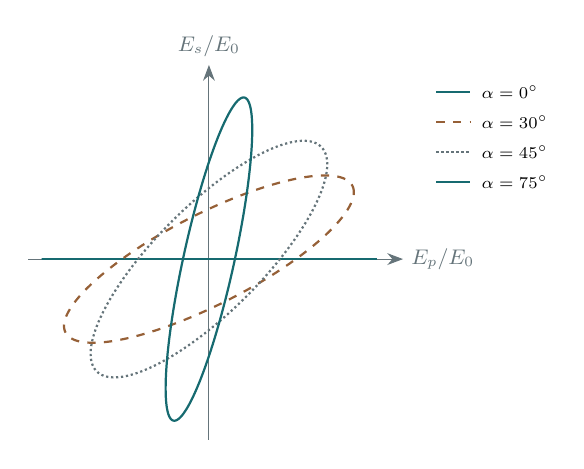
\begin{tikzpicture}[scale=.85,transform shape]
\draw[axis] (-2.7,0)--(2.9,0) node[right] {$E_p/E_0$};
\draw[axis] (0,-2.7)--(0,2.9) node[above] {$E_s/E_0$};
\draw[thick,color=accent] plot coordinates {(2.5000000,0.0000000) (2.4991433,0.0000000) (2.4965738,0.0000000) (2.4922933,0.0000000) (2.4863047,0.0000000) (2.4786122,0.0000000) (2.4692209,0.0000000) (2.4581373,0.0000000) (2.4453690,0.0000000) (2.4309248,0.0000000) (2.4148146,0.0000000) (2.3970493,0.0000000) (2.3776413,0.0000000) (2.3566037,0.0000000) (2.3339511,0.0000000) (2.3096988,0.0000000) (2.2838636,0.0000000) (2.2564632,0.0000000) (2.2275163,0.0000000) (2.1970428,0.0000000) (2.1650635,0.0000000) (2.1316004,0.0000000) (2.0966764,0.0000000) (2.0603155,0.0000000) (2.0225425,0.0000000) (1.9833834,0.0000000) (1.9428649,0.0000000) (1.9010149,0.0000000) (1.8578621,0.0000000) (1.8134359,0.0000000) (1.7677670,0.0000000) (1.7208864,0.0000000) (1.6728265,0.0000000) (1.6236201,0.0000000) (1.5733010,0.0000000) (1.5219036,0.0000000) (1.4694631,0.0000000) (1.4160156,0.0000000) (1.3615976,0.0000000) (1.3062464,0.0000000) (1.2500000,0.0000000) (1.1928969,0.0000000) (1.1349762,0.0000000) (1.0762777,0.0000000) (1.0168416,0.0000000) (0.9567086,0.0000000) (0.8959199,0.0000000) (0.8345171,0.0000000) (0.7725425,0.0000000) (0.7100384,0.0000000) (0.6470476,0.0000000) (0.5836134,0.0000000) (0.5197792,0.0000000) (0.4555888,0.0000000) (0.3910862,0.0000000) (0.3263155,0.0000000) (0.2613212,0.0000000) (0.1961477,0.0000000) (0.1308399,0.0000000) (0.0654424,0.0000000) (0.0000000,0.0000000) (-0.0654424,0.0000000) (-0.1308399,0.0000000) (-0.1961477,0.0000000) (-0.2613212,0.0000000) (-0.3263155,0.0000000) (-0.3910862,0.0000000) (-0.4555888,0.0000000) (-0.5197792,0.0000000) (-0.5836134,0.0000000) (-0.6470476,0.0000000) (-0.7100384,0.0000000) (-0.7725425,0.0000000) (-0.8345171,0.0000000) (-0.8959199,0.0000000) (-0.9567086,0.0000000) (-1.0168416,0.0000000) (-1.0762777,0.0000000) (-1.1349762,0.0000000) (-1.1928969,0.0000000) (-1.2500000,0.0000000) (-1.3062464,0.0000000) (-1.3615976,0.0000000) (-1.4160156,0.0000000) (-1.4694631,0.0000000) (-1.5219036,0.0000000) (-1.5733010,0.0000000) (-1.6236201,0.0000000) (-1.6728265,0.0000000) (-1.7208864,0.0000000) (-1.7677670,0.0000000) (-1.8134359,0.0000000) (-1.8578621,0.0000000) (-1.9010149,0.0000000) (-1.9428649,0.0000000) (-1.9833834,0.0000000) (-2.0225425,0.0000000) (-2.0603155,0.0000000) (-2.0966764,0.0000000) (-2.1316004,0.0000000) (-2.1650635,0.0000000) (-2.1970428,0.0000000) (-2.2275163,0.0000000) (-2.2564632,0.0000000) (-2.2838636,0.0000000) (-2.3096988,0.0000000) (-2.3339511,0.0000000) (-2.3566037,0.0000000) (-2.3776413,0.0000000) (-2.3970493,0.0000000) (-2.4148146,0.0000000) (-2.4309248,0.0000000) (-2.4453690,0.0000000) (-2.4581373,0.0000000) (-2.4692209,0.0000000) (-2.4786122,0.0000000) (-2.4863047,0.0000000) (-2.4922933,0.0000000) (-2.4965738,0.0000000) (-2.4991433,0.0000000) (-2.5000000,0.0000000) (-2.4991433,-0.0000000) (-2.4965738,-0.0000000) (-2.4922933,-0.0000000) (-2.4863047,-0.0000000) (-2.4786122,-0.0000000) (-2.4692209,-0.0000000) (-2.4581373,-0.0000000) (-2.4453690,-0.0000000) (-2.4309248,-0.0000000) (-2.4148146,-0.0000000) (-2.3970493,-0.0000000) (-2.3776413,-0.0000000) (-2.3566037,-0.0000000) (-2.3339511,-0.0000000) (-2.3096988,-0.0000000) (-2.2838636,-0.0000000) (-2.2564632,-0.0000000) (-2.2275163,-0.0000000) (-2.1970428,-0.0000000) (-2.1650635,-0.0000000) (-2.1316004,-0.0000000) (-2.0966764,-0.0000000) (-2.0603155,-0.0000000) (-2.0225425,-0.0000000) (-1.9833834,-0.0000000) (-1.9428649,-0.0000000) (-1.9010149,-0.0000000) (-1.8578621,-0.0000000) (-1.8134359,-0.0000000) (-1.7677670,-0.0000000) (-1.7208864,-0.0000000) (-1.6728265,-0.0000000) (-1.6236201,-0.0000000) (-1.5733010,-0.0000000) (-1.5219036,-0.0000000) (-1.4694631,-0.0000000) (-1.4160156,-0.0000000) (-1.3615976,-0.0000000) (-1.3062464,-0.0000000) (-1.2500000,-0.0000000) (-1.1928969,-0.0000000) (-1.1349762,-0.0000000) (-1.0762777,-0.0000000) (-1.0168416,-0.0000000) (-0.9567086,-0.0000000) (-0.8959199,-0.0000000) (-0.8345171,-0.0000000) (-0.7725425,-0.0000000) (-0.7100384,-0.0000000) (-0.6470476,-0.0000000) (-0.5836134,-0.0000000) (-0.5197792,-0.0000000) (-0.4555888,-0.0000000) (-0.3910862,-0.0000000) (-0.3263155,-0.0000000) (-0.2613212,-0.0000000) (-0.1961477,-0.0000000) (-0.1308399,-0.0000000) (-0.0654424,-0.0000000) (-0.0000000,-0.0000000) (0.0654424,0.0000000) (0.1308399,0.0000000) (0.1961477,0.0000000) (0.2613212,0.0000000) (0.3263155,0.0000000) (0.3910862,0.0000000) (0.4555888,0.0000000) (0.5197792,0.0000000) (0.5836134,0.0000000) (0.6470476,0.0000000) (0.7100384,0.0000000) (0.7725425,0.0000000) (0.8345171,0.0000000) (0.8959199,0.0000000) (0.9567086,0.0000000) (1.0168416,0.0000000) (1.0762777,0.0000000) (1.1349762,0.0000000) (1.1928969,0.0000000) (1.2500000,0.0000000) (1.3062464,0.0000000) (1.3615976,0.0000000) (1.4160156,0.0000000) (1.4694631,0.0000000) (1.5219036,0.0000000) (1.5733010,0.0000000) (1.6236201,0.0000000) (1.6728265,0.0000000) (1.7208864,0.0000000) (1.7677670,0.0000000) (1.8134359,0.0000000) (1.8578621,0.0000000) (1.9010149,0.0000000) (1.9428649,0.0000000) (1.9833834,0.0000000) (2.0225425,0.0000000) (2.0603155,0.0000000) (2.0966764,0.0000000) (2.1316004,0.0000000) (2.1650635,0.0000000) (2.1970428,0.0000000) (2.2275163,0.0000000) (2.2564632,0.0000000) (2.2838636,0.0000000) (2.3096988,0.0000000) (2.3339511,0.0000000) (2.3566037,0.0000000) (2.3776413,0.0000000) (2.3970493,0.0000000) (2.4148146,0.0000000) (2.4309248,0.0000000) (2.4453690,0.0000000) (2.4581373,0.0000000) (2.4692209,0.0000000) (2.4786122,0.0000000) (2.4863047,0.0000000) (2.4922933,0.0000000) (2.4965738,0.0000000) (2.4991433,0.0000000) (2.5000000,0.0000000)};
\draw[thick,color=accent] (3.4,2.5)--(3.9,2.5);\node[right,font=\scriptsize] at (3.95,2.5) {$\alpha=0^\circ$};
\draw[thick,dashed,color=warm] plot coordinates {(2.1650635,1.0000000) (2.1643216,1.0192900) (2.1620964,1.0378815) (2.1583893,1.0557617) (2.1532031,1.0729182) (2.1465411,1.0893395) (2.1384080,1.1050142) (2.1288093,1.1199316) (2.1177517,1.1340814) (2.1052426,1.1474539) (2.0912908,1.1600401) (2.0759056,1.1718312) (2.0590978,1.1828193) (2.0408787,1.1929966) (2.0212609,1.2023564) (2.0002579,1.2108921) (1.9778839,1.2185979) (1.9541545,1.2254686) (1.9290857,1.2314994) (1.9026949,1.2366862) (1.8750000,1.2410254) (1.8460201,1.2445141) (1.8157750,1.2471498) (1.7842855,1.2489309) (1.7515732,1.2498559) (1.7176604,1.2499244) (1.6825704,1.2491363) (1.6463272,1.2474920) (1.6089557,1.2449928) (1.5704816,1.2416403) (1.5309311,1.2374369) (1.4903314,1.2323854) (1.4487103,1.2264892) (1.4060963,1.2197525) (1.3625186,1.2121799) (1.3180072,1.2037764) (1.2725924,1.1945480) (1.2263055,1.1845009) (1.1791781,1.1736420) (1.1312426,1.1619787) (1.0825318,1.1495191) (1.0330790,1.1362716) (0.9829183,1.1222454) (0.9320839,1.1074501) (0.8806107,1.0918957) (0.8285339,1.0755931) (0.7758894,1.0585533) (0.7227131,1.0407880) (0.6690414,1.0223094) (0.6149113,1.0031301) (0.5603597,0.9832634) (0.5054240,0.9627228) (0.4501420,0.9415224) (0.3945515,0.9196767) (0.3386906,0.8972007) (0.2825975,0.8741098) (0.2263108,0.8504199) (0.1698689,0.8261471) (0.1133107,0.8013081) (0.0566748,0.7759199) (0.0000000,0.7500000) (-0.0566748,0.7235660) (-0.1133107,0.6966362) (-0.1698689,0.6692289) (-0.2263108,0.6413630) (-0.2825975,0.6130575) (-0.3386906,0.5843318) (-0.3945515,0.5552057) (-0.4501420,0.5256990) (-0.5054240,0.4958321) (-0.5603597,0.4656253) (-0.6149113,0.4350995) (-0.6690414,0.4042754) (-0.7227131,0.3731743) (-0.7758894,0.3418174) (-0.8285339,0.3102262) (-0.8806107,0.2784225) (-0.9320839,0.2464279) (-0.9829183,0.2142644) (-1.0330790,0.1819541) (-1.0825318,0.1495191) (-1.1312426,0.1169816) (-1.1791781,0.0843639) (-1.2263055,0.0516884) (-1.2725924,0.0189775) (-1.3180072,-0.0137464) (-1.3625186,-0.0464609) (-1.4060963,-0.0791436) (-1.4487103,-0.1117720) (-1.4903314,-0.1443238) (-1.5309311,-0.1767767) (-1.5704816,-0.2091084) (-1.6089557,-0.2412969) (-1.6463272,-0.2733199) (-1.6825704,-0.3051557) (-1.7176604,-0.3367823) (-1.7515732,-0.3681781) (-1.7842855,-0.3993215) (-1.8157750,-0.4301913) (-1.8460201,-0.4607662) (-1.8750000,-0.4910254) (-1.9026949,-0.5209480) (-1.9290857,-0.5505136) (-1.9541545,-0.5797020) (-1.9778839,-0.6084930) (-2.0002579,-0.6368670) (-2.0212609,-0.6648045) (-2.0408787,-0.6922863) (-2.0590978,-0.7192938) (-2.0759056,-0.7458082) (-2.0912908,-0.7718115) (-2.1052426,-0.7972859) (-2.1177517,-0.8222138) (-2.1288093,-0.8465783) (-2.1384080,-0.8703625) (-2.1465411,-0.8935502) (-2.1532031,-0.9161255) (-2.1583893,-0.9380730) (-2.1620964,-0.9593776) (-2.1643216,-0.9800246) (-2.1650635,-1.0000000) (-2.1643216,-1.0192900) (-2.1620964,-1.0378815) (-2.1583893,-1.0557617) (-2.1532031,-1.0729182) (-2.1465411,-1.0893395) (-2.1384080,-1.1050142) (-2.1288093,-1.1199316) (-2.1177517,-1.1340814) (-2.1052426,-1.1474539) (-2.0912908,-1.1600401) (-2.0759056,-1.1718312) (-2.0590978,-1.1828193) (-2.0408787,-1.1929966) (-2.0212609,-1.2023564) (-2.0002579,-1.2108921) (-1.9778839,-1.2185979) (-1.9541545,-1.2254686) (-1.9290857,-1.2314994) (-1.9026949,-1.2366862) (-1.8750000,-1.2410254) (-1.8460201,-1.2445141) (-1.8157750,-1.2471498) (-1.7842855,-1.2489309) (-1.7515732,-1.2498559) (-1.7176604,-1.2499244) (-1.6825704,-1.2491363) (-1.6463272,-1.2474920) (-1.6089557,-1.2449928) (-1.5704816,-1.2416403) (-1.5309311,-1.2374369) (-1.4903314,-1.2323854) (-1.4487103,-1.2264892) (-1.4060963,-1.2197525) (-1.3625186,-1.2121799) (-1.3180072,-1.2037764) (-1.2725924,-1.1945480) (-1.2263055,-1.1845009) (-1.1791781,-1.1736420) (-1.1312426,-1.1619787) (-1.0825318,-1.1495191) (-1.0330790,-1.1362716) (-0.9829183,-1.1222454) (-0.9320839,-1.1074501) (-0.8806107,-1.0918957) (-0.8285339,-1.0755931) (-0.7758894,-1.0585533) (-0.7227131,-1.0407880) (-0.6690414,-1.0223094) (-0.6149113,-1.0031301) (-0.5603597,-0.9832634) (-0.5054240,-0.9627228) (-0.4501420,-0.9415224) (-0.3945515,-0.9196767) (-0.3386906,-0.8972007) (-0.2825975,-0.8741098) (-0.2263108,-0.8504199) (-0.1698689,-0.8261471) (-0.1133107,-0.8013081) (-0.0566748,-0.7759199) (-0.0000000,-0.7500000) (0.0566748,-0.7235660) (0.1133107,-0.6966362) (0.1698689,-0.6692289) (0.2263108,-0.6413630) (0.2825975,-0.6130575) (0.3386906,-0.5843318) (0.3945515,-0.5552057) (0.4501420,-0.5256990) (0.5054240,-0.4958321) (0.5603597,-0.4656253) (0.6149113,-0.4350995) (0.6690414,-0.4042754) (0.7227131,-0.3731743) (0.7758894,-0.3418174) (0.8285339,-0.3102262) (0.8806107,-0.2784225) (0.9320839,-0.2464279) (0.9829183,-0.2142644) (1.0330790,-0.1819541) (1.0825318,-0.1495191) (1.1312426,-0.1169816) (1.1791781,-0.0843639) (1.2263055,-0.0516884) (1.2725924,-0.0189775) (1.3180072,0.0137464) (1.3625186,0.0464609) (1.4060963,0.0791436) (1.4487103,0.1117720) (1.4903314,0.1443238) (1.5309311,0.1767767) (1.5704816,0.2091084) (1.6089557,0.2412969) (1.6463272,0.2733199) (1.6825704,0.3051557) (1.7176604,0.3367823) (1.7515732,0.3681781) (1.7842855,0.3993215) (1.8157750,0.4301913) (1.8460201,0.4607662) (1.8750000,0.4910254) (1.9026949,0.5209480) (1.9290857,0.5505136) (1.9541545,0.5797020) (1.9778839,0.6084930) (2.0002579,0.6368670) (2.0212609,0.6648045) (2.0408787,0.6922863) (2.0590978,0.7192938) (2.0759056,0.7458082) (2.0912908,0.7718115) (2.1052426,0.7972859) (2.1177517,0.8222138) (2.1288093,0.8465783) (2.1384080,0.8703625) (2.1465411,0.8935502) (2.1532031,0.9161255) (2.1583893,0.9380730) (2.1620964,0.9593776) (2.1643216,0.9800246) (2.1650635,1.0000000)};
\draw[thick,dashed,color=warm] (3.4,2.05)--(3.9,2.05);\node[right,font=\scriptsize] at (3.95,2.05) {$\alpha=30^\circ$};
\draw[densely dotted,thick,color=muted] plot coordinates {(1.7677670,1.4142136) (1.7671612,1.4414938) (1.7653443,1.4677861) (1.7623175,1.4930725) (1.7580829,1.5173355) (1.7526435,1.5405587) (1.7460028,1.5627261) (1.7381655,1.5838224) (1.7291370,1.6038333) (1.7189234,1.6227449) (1.7075318,1.6405445) (1.6949698,1.6572196) (1.6812463,1.6727590) (1.6663705,1.6871520) (1.6503526,1.7003887) (1.6332037,1.7124600) (1.6149355,1.7233577) (1.5955604,1.7330743) (1.5750919,1.7416032) (1.5535438,1.7489384) (1.5309311,1.7550750) (1.5072691,1.7600087) (1.4825741,1.7637362) (1.4568630,1.7662550) (1.4301535,1.7675632) (1.4024638,1.7676601) (1.3738129,1.7665454) (1.3442205,1.7642201) (1.3137069,1.7606857) (1.2822928,1.7559446) (1.2500000,1.7500000) (1.2168505,1.7428561) (1.1828670,1.7345177) (1.1480728,1.7249906) (1.1124918,1.7142812) (1.0761483,1.7023970) (1.0390673,1.6893460) (1.0012742,1.6751372) (0.9627949,1.6597804) (0.9236557,1.6432860) (0.8838835,1.6256654) (0.8435055,1.6069307) (0.8025494,1.5870947) (0.7610433,1.5661709) (0.7190156,1.5441738) (0.6764951,1.5211183) (0.6335110,1.4970204) (0.5900927,1.4718965) (0.5462700,1.4457638) (0.5020729,1.4186403) (0.4575318,1.3905445) (0.4126770,1.3614956) (0.3675394,1.3315137) (0.3221499,1.3006193) (0.2765397,1.2688334) (0.2307399,1.2361780) (0.1847820,1.2026753) (0.1386974,1.1683484) (0.0925178,1.1332208) (0.0462747,1.0973165) (0.0000000,1.0606602) (-0.0462747,1.0232769) (-0.0925178,0.9851924) (-0.1386974,0.9464326) (-0.1847820,0.9070242) (-0.2307399,0.8669942) (-0.2765397,0.8263699) (-0.3221499,0.7851794) (-0.3675394,0.7434507) (-0.4126770,0.7012124) (-0.4575318,0.6584936) (-0.5020729,0.6153236) (-0.5462700,0.5717317) (-0.5900927,0.5277481) (-0.6335110,0.4834028) (-0.6764951,0.4387261) (-0.7190156,0.3937488) (-0.7610433,0.3485016) (-0.8025494,0.3030156) (-0.8435055,0.2573219) (-0.8838835,0.2114519) (-0.9236557,0.1654369) (-0.9627949,0.1193086) (-1.0012742,0.0730984) (-1.0390673,0.0268382) (-1.0761483,-0.0194404) (-1.1124918,-0.0657057) (-1.1480728,-0.1119259) (-1.1828670,-0.1580695) (-1.2168505,-0.2041047) (-1.2500000,-0.2500000) (-1.2822928,-0.2957240) (-1.3137069,-0.3412453) (-1.3442205,-0.3865328) (-1.3738129,-0.4315553) (-1.4024638,-0.4762821) (-1.4301535,-0.5206824) (-1.4568630,-0.5647259) (-1.4825741,-0.6083824) (-1.5072691,-0.6516219) (-1.5309311,-0.6944148) (-1.5535438,-0.7367318) (-1.5750919,-0.7785439) (-1.5955604,-0.8198224) (-1.6149355,-0.8605390) (-1.6332037,-0.9006659) (-1.6503526,-0.9401755) (-1.6663705,-0.9790407) (-1.6812463,-1.0172350) (-1.6949698,-1.0547321) (-1.7075318,-1.0915064) (-1.7189234,-1.1275325) (-1.7291370,-1.1627860) (-1.7381655,-1.1972425) (-1.7460028,-1.2308784) (-1.7526435,-1.2636708) (-1.7580829,-1.2955972) (-1.7623175,-1.3266356) (-1.7653443,-1.3567648) (-1.7671612,-1.3859641) (-1.7677670,-1.4142136) (-1.7671612,-1.4414938) (-1.7653443,-1.4677861) (-1.7623175,-1.4930725) (-1.7580829,-1.5173355) (-1.7526435,-1.5405587) (-1.7460028,-1.5627261) (-1.7381655,-1.5838224) (-1.7291370,-1.6038333) (-1.7189234,-1.6227449) (-1.7075318,-1.6405445) (-1.6949698,-1.6572196) (-1.6812463,-1.6727590) (-1.6663705,-1.6871520) (-1.6503526,-1.7003887) (-1.6332037,-1.7124600) (-1.6149355,-1.7233577) (-1.5955604,-1.7330743) (-1.5750919,-1.7416032) (-1.5535438,-1.7489384) (-1.5309311,-1.7550750) (-1.5072691,-1.7600087) (-1.4825741,-1.7637362) (-1.4568630,-1.7662550) (-1.4301535,-1.7675632) (-1.4024638,-1.7676601) (-1.3738129,-1.7665454) (-1.3442205,-1.7642201) (-1.3137069,-1.7606857) (-1.2822928,-1.7559446) (-1.2500000,-1.7500000) (-1.2168505,-1.7428561) (-1.1828670,-1.7345177) (-1.1480728,-1.7249906) (-1.1124918,-1.7142812) (-1.0761483,-1.7023970) (-1.0390673,-1.6893460) (-1.0012742,-1.6751372) (-0.9627949,-1.6597804) (-0.9236557,-1.6432860) (-0.8838835,-1.6256654) (-0.8435055,-1.6069307) (-0.8025494,-1.5870947) (-0.7610433,-1.5661709) (-0.7190156,-1.5441738) (-0.6764951,-1.5211183) (-0.6335110,-1.4970204) (-0.5900927,-1.4718965) (-0.5462700,-1.4457638) (-0.5020729,-1.4186403) (-0.4575318,-1.3905445) (-0.4126770,-1.3614956) (-0.3675394,-1.3315137) (-0.3221499,-1.3006193) (-0.2765397,-1.2688334) (-0.2307399,-1.2361780) (-0.1847820,-1.2026753) (-0.1386974,-1.1683484) (-0.0925178,-1.1332208) (-0.0462747,-1.0973165) (-0.0000000,-1.0606602) (0.0462747,-1.0232769) (0.0925178,-0.9851924) (0.1386974,-0.9464326) (0.1847820,-0.9070242) (0.2307399,-0.8669942) (0.2765397,-0.8263699) (0.3221499,-0.7851794) (0.3675394,-0.7434507) (0.4126770,-0.7012124) (0.4575318,-0.6584936) (0.5020729,-0.6153236) (0.5462700,-0.5717317) (0.5900927,-0.5277481) (0.6335110,-0.4834028) (0.6764951,-0.4387261) (0.7190156,-0.3937488) (0.7610433,-0.3485016) (0.8025494,-0.3030156) (0.8435055,-0.2573219) (0.8838835,-0.2114519) (0.9236557,-0.1654369) (0.9627949,-0.1193086) (1.0012742,-0.0730984) (1.0390673,-0.0268382) (1.0761483,0.0194404) (1.1124918,0.0657057) (1.1480728,0.1119259) (1.1828670,0.1580695) (1.2168505,0.2041047) (1.2500000,0.2500000) (1.2822928,0.2957240) (1.3137069,0.3412453) (1.3442205,0.3865328) (1.3738129,0.4315553) (1.4024638,0.4762821) (1.4301535,0.5206824) (1.4568630,0.5647259) (1.4825741,0.6083824) (1.5072691,0.6516219) (1.5309311,0.6944148) (1.5535438,0.7367318) (1.5750919,0.7785439) (1.5955604,0.8198224) (1.6149355,0.8605390) (1.6332037,0.9006659) (1.6503526,0.9401755) (1.6663705,0.9790407) (1.6812463,1.0172350) (1.6949698,1.0547321) (1.7075318,1.0915064) (1.7189234,1.1275325) (1.7291370,1.1627860) (1.7381655,1.1972425) (1.7460028,1.2308784) (1.7526435,1.2636708) (1.7580829,1.2955972) (1.7623175,1.3266356) (1.7653443,1.3567648) (1.7671612,1.3859641) (1.7677670,1.4142136)};
\draw[densely dotted,thick,color=muted] (3.4,1.6)--(3.9,1.6);\node[right,font=\scriptsize] at (3.95,1.6) {$\alpha=45^\circ$};
\draw[thick,color=accent] plot coordinates {(0.6470476,1.9318517) (0.6468259,1.9691171) (0.6461609,2.0050331) (0.6450530,2.0395749) (0.6435030,2.0727189) (0.6415120,2.1044423) (0.6390814,2.1347235) (0.6362127,2.1635416) (0.6329081,2.1908770) (0.6291696,2.2167108) (0.6250000,2.2410254) (0.6204020,2.2638041) (0.6153788,2.2850313) (0.6099339,2.3046925) (0.6040710,2.3227742) (0.5977940,2.3392639) (0.5911074,2.3541504) (0.5840157,2.3674236) (0.5765236,2.3790741) (0.5686365,2.3890942) (0.5603597,2.3974770) (0.5516988,2.4042166) (0.5426598,2.4093085) (0.5332489,2.4127492) (0.5234725,2.4145363) (0.5133374,2.4146685) (0.5028504,2.4131459) (0.4920189,2.4099695) (0.4808501,2.4051414) (0.4693518,2.3986649) (0.4575318,2.3905445) (0.4453982,2.3807857) (0.4329594,2.3693952) (0.4202238,2.3563809) (0.4072003,2.3417517) (0.3938976,2.3255175) (0.3803250,2.3076895) (0.3664918,2.2882800) (0.3524074,2.2673022) (0.3380814,2.2447704) (0.3235238,2.2207003) (0.3087444,2.1951082) (0.2937535,2.1680116) (0.2785612,2.1394292) (0.2631780,2.1093806) (0.2476144,2.0778863) (0.2318811,2.0449679) (0.2159889,2.0106480) (0.1999487,1.9749501) (0.1837715,1.9378986) (0.1674682,1.8995191) (0.1510503,1.8598376) (0.1345288,1.8188816) (0.1179151,1.7766790) (0.1012205,1.7332587) (0.0844567,1.6886505) (0.0676349,1.6428851) (0.0507668,1.5959936) (0.0338639,1.5480084) (0.0169377,1.4989622) (0.0000000,1.4488887) (-0.0169377,1.3978223) (-0.0338639,1.3457978) (-0.0507668,1.2928510) (-0.0676349,1.2390181) (-0.0844567,1.1843361) (-0.1012205,1.1288423) (-0.1179151,1.0725750) (-0.1345288,1.0155725) (-0.1510503,0.9578740) (-0.1674682,0.8995191) (-0.1837715,0.8405476) (-0.1999487,0.7810001) (-0.2159889,0.7209173) (-0.2318811,0.6603405) (-0.2476144,0.5993110) (-0.2631780,0.5378709) (-0.2785612,0.4760621) (-0.2937535,0.4139270) (-0.3087444,0.3515083) (-0.3235238,0.2888486) (-0.3380814,0.2259910) (-0.3524074,0.1629785) (-0.3664918,0.0998543) (-0.3803250,0.0366617) (-0.3938976,-0.0265561) (-0.4072003,-0.0897556) (-0.4202238,-0.1528936) (-0.4329594,-0.2159269) (-0.4453982,-0.2788122) (-0.4575318,-0.3415064) (-0.4693518,-0.4039665) (-0.4808501,-0.4661498) (-0.4920189,-0.5280136) (-0.5028504,-0.5895155) (-0.5133374,-0.6506134) (-0.5234725,-0.7112654) (-0.5332489,-0.7714299) (-0.5426598,-0.8310658) (-0.5516988,-0.8901320) (-0.5603597,-0.9485882) (-0.5686365,-1.0063943) (-0.5765236,-1.0635107) (-0.5840157,-1.1198982) (-0.5911074,-1.1755182) (-0.5977940,-1.2303325) (-0.6040710,-1.2843036) (-0.6099339,-1.3373945) (-0.6153788,-1.3895689) (-0.6204020,-1.4407909) (-0.6250000,-1.4910254) (-0.6291696,-1.5402381) (-0.6329081,-1.5883952) (-0.6362127,-1.6354636) (-0.6390814,-1.6814112) (-0.6415120,-1.7262065) (-0.6435030,-1.7698187) (-0.6450530,-1.8122179) (-0.6461609,-1.8533751) (-0.6468259,-1.8932622) (-0.6470476,-1.9318517) (-0.6468259,-1.9691171) (-0.6461609,-2.0050331) (-0.6450530,-2.0395749) (-0.6435030,-2.0727189) (-0.6415120,-2.1044423) (-0.6390814,-2.1347235) (-0.6362127,-2.1635416) (-0.6329081,-2.1908770) (-0.6291696,-2.2167108) (-0.6250000,-2.2410254) (-0.6204020,-2.2638041) (-0.6153788,-2.2850313) (-0.6099339,-2.3046925) (-0.6040710,-2.3227742) (-0.5977940,-2.3392639) (-0.5911074,-2.3541504) (-0.5840157,-2.3674236) (-0.5765236,-2.3790741) (-0.5686365,-2.3890942) (-0.5603597,-2.3974770) (-0.5516988,-2.4042166) (-0.5426598,-2.4093085) (-0.5332489,-2.4127492) (-0.5234725,-2.4145363) (-0.5133374,-2.4146685) (-0.5028504,-2.4131459) (-0.4920189,-2.4099695) (-0.4808501,-2.4051414) (-0.4693518,-2.3986649) (-0.4575318,-2.3905445) (-0.4453982,-2.3807857) (-0.4329594,-2.3693952) (-0.4202238,-2.3563809) (-0.4072003,-2.3417517) (-0.3938976,-2.3255175) (-0.3803250,-2.3076895) (-0.3664918,-2.2882800) (-0.3524074,-2.2673022) (-0.3380814,-2.2447704) (-0.3235238,-2.2207003) (-0.3087444,-2.1951082) (-0.2937535,-2.1680116) (-0.2785612,-2.1394292) (-0.2631780,-2.1093806) (-0.2476144,-2.0778863) (-0.2318811,-2.0449679) (-0.2159889,-2.0106480) (-0.1999487,-1.9749501) (-0.1837715,-1.9378986) (-0.1674682,-1.8995191) (-0.1510503,-1.8598376) (-0.1345288,-1.8188816) (-0.1179151,-1.7766790) (-0.1012205,-1.7332587) (-0.0844567,-1.6886505) (-0.0676349,-1.6428851) (-0.0507668,-1.5959936) (-0.0338639,-1.5480084) (-0.0169377,-1.4989622) (-0.0000000,-1.4488887) (0.0169377,-1.3978223) (0.0338639,-1.3457978) (0.0507668,-1.2928510) (0.0676349,-1.2390181) (0.0844567,-1.1843361) (0.1012205,-1.1288423) (0.1179151,-1.0725750) (0.1345288,-1.0155725) (0.1510503,-0.9578740) (0.1674682,-0.8995191) (0.1837715,-0.8405476) (0.1999487,-0.7810001) (0.2159889,-0.7209173) (0.2318811,-0.6603405) (0.2476144,-0.5993110) (0.2631780,-0.5378709) (0.2785612,-0.4760621) (0.2937535,-0.4139270) (0.3087444,-0.3515083) (0.3235238,-0.2888486) (0.3380814,-0.2259910) (0.3524074,-0.1629785) (0.3664918,-0.0998543) (0.3803250,-0.0366617) (0.3938976,0.0265561) (0.4072003,0.0897556) (0.4202238,0.1528936) (0.4329594,0.2159269) (0.4453982,0.2788122) (0.4575318,0.3415064) (0.4693518,0.4039665) (0.4808501,0.4661498) (0.4920189,0.5280136) (0.5028504,0.5895155) (0.5133374,0.6506134) (0.5234725,0.7112654) (0.5332489,0.7714299) (0.5426598,0.8310658) (0.5516988,0.8901320) (0.5603597,0.9485882) (0.5686365,1.0063943) (0.5765236,1.0635107) (0.5840157,1.1198982) (0.5911074,1.1755182) (0.5977940,1.2303325) (0.6040710,1.2843036) (0.6099339,1.3373945) (0.6153788,1.3895689) (0.6204020,1.4407909) (0.6250000,1.4910254) (0.6291696,1.5402381) (0.6329081,1.5883952) (0.6362127,1.6354636) (0.6390814,1.6814112) (0.6415120,1.7262065) (0.6435030,1.7698187) (0.6450530,1.8122179) (0.6461609,1.8533751) (0.6468259,1.8932622) (0.6470476,1.9318517)};
\draw[thick,color=accent] (3.4,1.15)--(3.9,1.15);\node[right,font=\scriptsize] at (3.95,1.15) {$\alpha=75^\circ$};
\end{tikzpicture}
\figcaption{解图光4.8C\quad 玻璃到空气45度全反射，不同入射方位给不同电场轨迹}
\end{minipage}\end{center}
纯$p$或纯$s$入射只有一个振动方向，反射仍为线偏振；此时直接使用单分量场式。临界角或掠入射的极限使$\delta\to0$，两非零分量也合成直线。对题设严格全反射区间和正折射率，两个非零分量形成椭圆；等幅且$\delta=\pi/2$时形成圆。

为了确定全反射延迟器的可用范围，令$x=\sin^2\theta$，由相位差式有
\[
\tan^2\frac\delta2=\frac{(1-x)(x-m^2)}{x^2}.
\]
将右侧展开为$-1+(1+m^2)/x-m^2/x^2$，求导得
\[
 \frac{d}{dx}\tan^2\frac\delta2
 =\frac{2m^2-(1+m^2)x}{x^3}.
\]
在$m^2<x<1$内，导数由正变负，最大值位于$x_*=2m^2/(1+m^2)$，代回得
\[
 \boxed{\delta_{\max}=2\arctan\frac{1-m^2}{2m}},\qquad
 \theta_*=\arcsin\sqrt{\frac{2m^2}{1+m^2}}.
\]
解图光4.8D显示最大延迟随折射率比增加而增大。以$n_1/n_2=1.5$为例，$\theta_*=51.67118^\circ$、$\delta_{\max}=45.23973^\circ$；两次同面全反射可积累$90^\circ$相对相位，而保持每一分量的功率。
\begin{center}\begin{minipage}{.98\linewidth}\centering
\begin{tikzpicture}[scale=.88,transform shape]
\draw[axis] (0,0.0)--(7.3,0.0) node[right] {$n_1/n_2$};
\draw[axis] (0,0)--(0,2.8);
\node[above left] at (0,2.8) {$\delta_{\max}/{}^\circ$};
\draw[thin] (0.000000,0.0)--(0.000000,-0.06);\node[below,font=\scriptsize] at (0.000000,-0.08) {$ 1 $};
\draw[thin] (1.750000,0.0)--(1.750000,-0.06);\node[below,font=\scriptsize] at (1.750000,-0.08) {$ 1.5 $};
\draw[thin] (3.500000,0.0)--(3.500000,-0.06);\node[below,font=\scriptsize] at (3.500000,-0.08) {$ 2 $};
\draw[thin] (4.949749,0.0)--(4.949749,-0.06);\node[below,font=\scriptsize] at (4.949749,-0.08) {$ 2.41421 $};
\draw[thin] (7.000000,0.0)--(7.000000,-0.06);\node[below,font=\scriptsize] at (7.000000,-0.08) {$ 3 $};
\draw[thin] (0,0.000000)--(-.06,0.000000);\node[left,font=\scriptsize] at (-.08,0.000000) {$ 0 $};
\draw[thin] (0,1.022727)--(-.06,1.022727);\node[left,font=\scriptsize] at (-.08,1.022727) {$ 45 $};
\draw[thin] (0,2.045455)--(-.06,2.045455);\node[left,font=\scriptsize] at (-.08,2.045455) {$ 90 $};
\draw[thick,color=accent] plot coordinates {(0.0000000,0.0000000) (0.0291667,0.0216128) (0.0583333,0.0430462) (0.0875000,0.0643018) (0.1166667,0.0853810) (0.1458333,0.1062854) (0.1750000,0.1270165) (0.2041667,0.1475757) (0.2333333,0.1679646) (0.2625000,0.1881846) (0.2916667,0.2082373) (0.3208333,0.2281241) (0.3500000,0.2478465) (0.3791667,0.2674059) (0.4083333,0.2868039) (0.4375000,0.3060419) (0.4666667,0.3251213) (0.4958333,0.3440436) (0.5250000,0.3628103) (0.5541667,0.3814227) (0.5833333,0.3998823) (0.6125000,0.4181905) (0.6416667,0.4363487) (0.6708333,0.4543584) (0.7000000,0.4722208) (0.7291667,0.4899374) (0.7583333,0.5075096) (0.7875000,0.5249387) (0.8166667,0.5422261) (0.8458333,0.5593731) (0.8750000,0.5763811) (0.9041667,0.5932513) (0.9333333,0.6099852) (0.9625000,0.6265839) (0.9916667,0.6430489) (1.0208333,0.6593813) (1.0500000,0.6755825) (1.0791667,0.6916538) (1.1083333,0.7075963) (1.1375000,0.7234114) (1.1666667,0.7391002) (1.1958333,0.7546640) (1.2250000,0.7701041) (1.2541667,0.7854215) (1.2833333,0.8006175) (1.3125000,0.8156933) (1.3416667,0.8306501) (1.3708333,0.8454890) (1.4000000,0.8602111) (1.4291667,0.8748177) (1.4583333,0.8893097) (1.4875000,0.9036885) (1.5166667,0.9179549) (1.5458333,0.9321103) (1.5750000,0.9461556) (1.6041667,0.9600919) (1.6333333,0.9739203) (1.6625000,0.9876418) (1.6916667,1.0012575) (1.7208333,1.0147685) (1.7500000,1.0281757) (1.7791667,1.0414801) (1.8083333,1.0546829) (1.8375000,1.0677849) (1.8666667,1.0807871) (1.8958333,1.0936906) (1.9250000,1.1064962) (1.9541667,1.1192050) (1.9833333,1.1318179) (2.0125000,1.1443358) (2.0416667,1.1567596) (2.0708333,1.1690903) (2.1000000,1.1813288) (2.1291667,1.1934759) (2.1583333,1.2055327) (2.1875000,1.2174998) (2.2166667,1.2293782) (2.2458333,1.2411689) (2.2750000,1.2528725) (2.3041667,1.2644900) (2.3333333,1.2760221) (2.3625000,1.2874698) (2.3916667,1.2988338) (2.4208333,1.3101150) (2.4500000,1.3213141) (2.4791667,1.3324319) (2.5083333,1.3434692) (2.5375000,1.3544269) (2.5666667,1.3653055) (2.5958333,1.3761060) (2.6250000,1.3868290) (2.6541667,1.3974753) (2.6833333,1.4080456) (2.7125000,1.4185406) (2.7416667,1.4289612) (2.7708333,1.4393079) (2.8000000,1.4495814) (2.8291667,1.4597826) (2.8583333,1.4699120) (2.8875000,1.4799703) (2.9166667,1.4899582) (2.9458333,1.4998764) (2.9750000,1.5097255) (3.0041667,1.5195062) (3.0333333,1.5292191) (3.0625000,1.5388648) (3.0916667,1.5484440) (3.1208333,1.5579574) (3.1500000,1.5674054) (3.1791667,1.5767888) (3.2083333,1.5861080) (3.2375000,1.5953638) (3.2666667,1.6045567) (3.2958333,1.6136873) (3.3250000,1.6227562) (3.3541667,1.6317639) (3.3833333,1.6407110) (3.4125000,1.6495981) (3.4416667,1.6584256) (3.4708333,1.6671942) (3.5000000,1.6759044) (3.5291667,1.6845568) (3.5583333,1.6931518) (3.5875000,1.7016899) (3.6166667,1.7101718) (3.6458333,1.7185978) (3.6750000,1.7269686) (3.7041667,1.7352845) (3.7333333,1.7435462) (3.7625000,1.7517540) (3.7916667,1.7599086) (3.8208333,1.7680102) (3.8500000,1.7760595) (3.8791667,1.7840569) (3.9083333,1.7920029) (3.9375000,1.7998979) (3.9666667,1.8077423) (3.9958333,1.8155366) (4.0250000,1.8232813) (4.0541667,1.8309768) (4.0833333,1.8386236) (4.1125000,1.8462220) (4.1416667,1.8537725) (4.1708333,1.8612755) (4.2000000,1.8687314) (4.2291667,1.8761406) (4.2583333,1.8835036) (4.2875000,1.8908208) (4.3166667,1.8980924) (4.3458333,1.9053191) (4.3750000,1.9125010) (4.4041667,1.9196387) (4.4333333,1.9267324) (4.4625000,1.9337826) (4.4916667,1.9407897) (4.5208333,1.9477540) (4.5500000,1.9546758) (4.5791667,1.9615557) (4.6083333,1.9683938) (4.6375000,1.9751905) (4.6666667,1.9819463) (4.6958333,1.9886614) (4.7250000,1.9953363) (4.7541667,2.0019711) (4.7833333,2.0085664) (4.8125000,2.0151223) (4.8416667,2.0216393) (4.8708333,2.0281177) (4.9000000,2.0345577) (4.9291667,2.0409598) (4.9583333,2.0473241) (4.9875000,2.0536511) (5.0166667,2.0599411) (5.0458333,2.0661943) (5.0750000,2.0724110) (5.1041667,2.0785916) (5.1333333,2.0847364) (5.1625000,2.0908456) (5.1916667,2.0969195) (5.2208333,2.1029585) (5.2500000,2.1089628) (5.2791667,2.1149326) (5.3083333,2.1208684) (5.3375000,2.1267703) (5.3666667,2.1326386) (5.3958333,2.1384735) (5.4250000,2.1442755) (5.4541667,2.1500447) (5.4833333,2.1557814) (5.5125000,2.1614858) (5.5416667,2.1671582) (5.5708333,2.1727989) (5.6000000,2.1784081) (5.6291667,2.1839861) (5.6583333,2.1895330) (5.6875000,2.1950493) (5.7166667,2.2005350) (5.7458333,2.2059905) (5.7750000,2.2114159) (5.8041667,2.2168116) (5.8333333,2.2221777) (5.8625000,2.2275145) (5.8916667,2.2328222) (5.9208333,2.2381010) (5.9500000,2.2433512) (5.9791667,2.2485730) (6.0083333,2.2537665) (6.0375000,2.2589321) (6.0666667,2.2640699) (6.0958333,2.2691801) (6.1250000,2.2742630) (6.1541667,2.2793188) (6.1833333,2.2843477) (6.2125000,2.2893498) (6.2416667,2.2943254) (6.2708333,2.2992747) (6.3000000,2.3041978) (6.3291667,2.3090951) (6.3583333,2.3139666) (6.3875000,2.3188126) (6.4166667,2.3236332) (6.4458333,2.3284287) (6.4750000,2.3331992) (6.5041667,2.3379450) (6.5333333,2.3426661) (6.5625000,2.3473629) (6.5916667,2.3520354) (6.6208333,2.3566839) (6.6500000,2.3613085) (6.6791667,2.3659095) (6.7083333,2.3704869) (6.7375000,2.3750409) (6.7666667,2.3795718) (6.7958333,2.3840797) (6.8250000,2.3885647) (6.8541667,2.3930271) (6.8833333,2.3974670) (6.9125000,2.4018845) (6.9416667,2.4062799) (6.9708333,2.4106532) (7.0000000,2.4150047)};
\end{tikzpicture}
\figcaption{解图光4.8D\quad 最大单次相位差随折射率反差增加}
\end{minipage}\end{center}


\Needspace{13\baselineskip}

\pdfbookmark[2]{第 9 题 由椭偏反射比求折射率}{q9}

\section*{第 9 题\quad 由椭偏反射比求折射率}\label{q:9}

线偏振光以已知角$\theta$从折射率$n_1$的透明非磁介质射向均匀、各向同性、非磁性的半无限介质。实验得到复振幅反射系数之比$G=r_p/r_s$。推导由$G$求第二介质复折射率$N$的公式，并讨论解的选取与测量退化。采用时间因子$e^{-i\omega t}$。

\begin{center}\begin{minipage}{.98\linewidth}\centering
\begin{tikzpicture}[scale=.9,transform shape]
\draw[object] (-3.10000,0.00000)--(3.50000,0.00000);\draw[guide] (0.00000,-2.50000)--(0.00000,2.70000);\fill (0.00000,0.00000) circle(.035);\node[above right] at (0.00000,0.00000) {$O$};\draw[motion] (-1.76777,1.76777)--(0.00000,0.00000);
\draw[motion] (0.00000,0.00000)--(1.76777,1.76777);\draw[motion] (0.00000,0.00000)--(1.17851,-2.20479);\node[right] at (-2.90000,1.50000) {$n_1$};\node[right] at (-2.90000,-1.50000) {$N$};\node[left] at (-0.50000,1.00000) {$\theta_i$};\node[right] at (0.55000,1.10000) {$\theta_r$};\node[right] at (0.42000,-1.00000) {$\operatorname{Re}\boldsymbol k$};\node[right] at (3.00000,-2.30000) {可含吸收介质};
\end{tikzpicture}
\figcaption{图光4.9\quad 入射、反射及介质内相位方向示意}
\end{minipage}\end{center}

\Needspace{6\baselineskip}\subsection*{解答}


图光4.9中第一介质透明，第二介质均匀、各向同性、非磁且占据整个透射半空间。取$z$正向进入第二介质，时间因子为$e^{-i\omega t}$，每束光的$p$方向为$\boldsymbol s\times\hat{\boldsymbol k}$。实验复比$G$按这一有向约定定义。令$k_0$为真空波数，第二介质的法向波矢为$k_0q_z$，切向连续使$k_x/k_0=n_1\sin\theta$，故
\[
q_z^2=N^2-n_1^2\sin^2\theta.
\]
透明传播情形取向内输送能量的根；有吸收时取使$e^{ik_0q_zz}$随深度衰减的根，即$\operatorname{Im}q_z>0$。以$q_z=N\cos\theta_t$改写两偏振的菲涅耳系数：
\[
r_s=\frac{n_1\cos\theta-q_z}{n_1\cos\theta+q_z},\qquad
r_p=\frac{N^2\cos\theta-n_1q_z}{N^2\cos\theta+n_1q_z}.
\]
解图光4.9A给出$N=1.5+0.2i$、$n_1=1$、$\theta=60^\circ$的一例。左侧画实相位波矢的分量，虚法向分量单独写成衰减因子，右侧画实际测得的复比；吸收信息进入两个分量的相对相位。
\begin{center}\begin{minipage}{.98\linewidth}\centering
\begin{tikzpicture}[scale=.86,transform shape]
\draw[axis] (0,0)--(3.1,0) node[right] {$x$};\draw[axis] (0,0)--(0,3.1) node[above] {$z$};
\draw[motion] (0,0)--(1.7320508,0);\draw[motion] (1.7320508,0)--(1.7320508,2.4651492);\draw[motion] (0,0)--(1.7320508,2.4651492);
\node[below] at (.86,-.05) {$k_x/k_0=.866025$};\node[right,font=\small] at (1.8,1.3) {$\operatorname{Re}q_z=1.232575$};
\node[below,font=\small] at (1.5,-.7) {$e^{-.243393 k_0z}$；法向衰减};
\begin{scope}[shift={(7,1.3)}]\draw[axis] (-1.7,0)--(1.9,0) node[right] {$\operatorname{Re}G$};\draw[axis] (0,-1.7)--(0,1.9) node[above] {$\operatorname{Im}G$};
\draw[motion] (0,0)--(0.7137938,-0.7761458);
\draw (.8,-.04)--(.8,.04) node[above] {$0.1$};\draw (-.04,-.8)--(.04,-.8) node[left] {$-0.1$};
\node[below right,font=\small] at (.75,-.8) {$G=.089224-.097018i$};\end{scope}
\end{tikzpicture}
\figcaption{解图光4.9A\quad 60度入射的实相位分量、法向衰减与复反射比}
\end{minipage}\end{center}
为完整展开消元，记$c=\cos\theta$、$s=\sin\theta$、$u=\cos\theta_t=q_z/N$。将$G=r_p/r_s$交叉相乘，并把含$1-G$与$1+G$的项分组，得到
\[
 (N^2-n_1^2)cu+n_1N(c^2-u^2)\frac{1-G}{1+G}=0.
\]
这里使用$G\ne-1$，参考反射分量$r_s$有可测的非零值。由$u^2=1-n_1^2s^2/N^2$可得$c^2-u^2=(n_1^2-N^2)s^2/N^2$，再乘$N$整理为
\[
 (N^2-n_1^2)\left[cq_z-n_1s^2\frac{1-G}{1+G}\right]=0.
\]
折射率匹配$N=n_1$时两个反射系数同时为零，$G$无定义；对有反射、$0<\theta<\pi/2$的测量，由中括号为零得到
\[
G=\frac{n_1\sin\theta\tan\theta-q_z}
{n_1\sin\theta\tan\theta+q_z},
\quad
q_z=n_1\sin\theta\tan\theta\frac{1-G}{1+G}.
\]
这一步直接给出$q_z$的符号和复相位。把它代回第一式并平方，有
\[
\boxed{N^2=n_1^2\sin^2\theta\left[1+\tan^2\theta
\left(\frac{1-G}{1+G}\right)^2\right]}.
\]
于是$N=n_1\sin\theta\sqrt{1+\tan^2\theta[(1-G)/(1+G)]^2}$。对于通常的被动非磁介质，取$\operatorname{Re}N\geqslant0$、$\operatorname{Im}N\geqslant0$且与正实折射率连续的分支，同时要求未平方的$q_z$具有向内传播或衰减的方向。平方关系给出$N^2$，未平方关系保留传播方向，两者共同确定物理解。

解图光4.9B显示同一吸收介质的$\operatorname{Re}G,\operatorname{Im}G$随角度变化；$G=\tan\Psi\,e^{i\Delta}$中的$\Psi$和$\Delta$提供两个实测量，分别携带相对振幅和相位。用$|G|$或强度比$|G|^2$代入会丢去$\Delta$。在$60^\circ$一例中，
\[
 G=0.0892242-0.0970182i,\quad
 q_z=1.2325746+0.2433930i,\quad
 N^2=2.21+0.60i,\quad N=1.5+0.2i.
\]
由此计算的两菲涅耳系数分别为$r_s=-0.4339943-0.0795128i$、$r_p=-0.0464370+0.0350109i$，两者之比恢复上述复比。
\begin{center}\begin{minipage}{.98\linewidth}\centering
\begin{tikzpicture}[scale=.88,transform shape]
\draw[axis] (0,1.25)--(7.3,1.25) node[right] {$\theta/{}^\circ$};
\draw[axis] (0,0)--(0,2.8);
\node[above left] at (0,2.8) {$G\text{的分量}$};
\draw[thin] (0.000000,1.25)--(0.000000,1.19);\node[below,font=\scriptsize] at (0.000000,1.17) {$ 10 $};
\draw[thin] (1.866667,1.25)--(1.866667,1.19);\node[below,font=\scriptsize] at (1.866667,1.17) {$ 30 $};
\draw[thin] (3.266667,1.25)--(3.266667,1.19);\node[below,font=\scriptsize] at (3.266667,1.17) {$ 45 $};
\draw[thin] (4.666667,1.25)--(4.666667,1.19);\node[below,font=\scriptsize] at (4.666667,1.17) {$ 60 $};
\draw[thin] (6.066667,1.25)--(6.066667,1.19);\node[below,font=\scriptsize] at (6.066667,1.17) {$ 75 $};
\draw[thin] (7.000000,1.25)--(7.000000,1.19);\node[below,font=\scriptsize] at (7.000000,1.17) {$ 85 $};
\draw[thin] (0,0.000000)--(-.06,0.000000);\node[left,font=\scriptsize] at (-.08,0.000000) {$ -1 $};
\draw[thin] (0,0.625000)--(-.06,0.625000);\node[left,font=\scriptsize] at (-.08,0.625000) {$ -0.5 $};
\draw[thin] (0,1.250000)--(-.06,1.250000);\node[left,font=\scriptsize] at (-.08,1.250000) {$ 0 $};
\draw[thin] (0,1.875000)--(-.06,1.875000);\node[left,font=\scriptsize] at (-.08,1.875000) {$ 0.5 $};
\draw[thin] (0,2.500000)--(-.06,2.500000);\node[left,font=\scriptsize] at (-.08,2.500000) {$ 1 $};
\draw[thick,color=accent] plot coordinates {(0.0000000,0.0494693) (0.0291667,0.0525817) (0.0583333,0.0557864) (0.0875000,0.0590831) (0.1166667,0.0624715) (0.1458333,0.0659513) (0.1750000,0.0695221) (0.2041667,0.0731837) (0.2333333,0.0769355) (0.2625000,0.0807773) (0.2916667,0.0847088) (0.3208333,0.0887294) (0.3500000,0.0928389) (0.3791667,0.0970369) (0.4083333,0.1013229) (0.4375000,0.1056966) (0.4666667,0.1101575) (0.4958333,0.1147052) (0.5250000,0.1193393) (0.5541667,0.1240593) (0.5833333,0.1288648) (0.6125000,0.1337553) (0.6416667,0.1387304) (0.6708333,0.1437895) (0.7000000,0.1489323) (0.7291667,0.1541583) (0.7583333,0.1594668) (0.7875000,0.1648575) (0.8166667,0.1703299) (0.8458333,0.1758834) (0.8750000,0.1815175) (0.9041667,0.1872316) (0.9333333,0.1930253) (0.9625000,0.1988981) (0.9916667,0.2048492) (1.0208333,0.2108783) (1.0500000,0.2169848) (1.0791667,0.2231680) (1.1083333,0.2294275) (1.1375000,0.2357626) (1.1666667,0.2421728) (1.1958333,0.2486574) (1.2250000,0.2552159) (1.2541667,0.2618477) (1.2833333,0.2685522) (1.3125000,0.2753287) (1.3416667,0.2821767) (1.3708333,0.2890956) (1.4000000,0.2960846) (1.4291667,0.3031433) (1.4583333,0.3102708) (1.4875000,0.3174667) (1.5166667,0.3247303) (1.5458333,0.3320609) (1.5750000,0.3394578) (1.6041667,0.3469204) (1.6333333,0.3544482) (1.6625000,0.3620403) (1.6916667,0.3696961) (1.7208333,0.3774149) (1.7500000,0.3851962) (1.7791667,0.3930391) (1.8083333,0.4009431) (1.8375000,0.4089074) (1.8666667,0.4169314) (1.8958333,0.4250143) (1.9250000,0.4331555) (1.9541667,0.4413542) (1.9833333,0.4496099) (2.0125000,0.4579217) (2.0416667,0.4662890) (2.0708333,0.4747111) (2.1000000,0.4831872) (2.1291667,0.4917167) (2.1583333,0.5002989) (2.1875000,0.5089330) (2.2166667,0.5176184) (2.2458333,0.5263542) (2.2750000,0.5351399) (2.3041667,0.5439747) (2.3333333,0.5528579) (2.3625000,0.5617887) (2.3916667,0.5707666) (2.4208333,0.5797906) (2.4500000,0.5888602) (2.4791667,0.5979746) (2.5083333,0.6071331) (2.5375000,0.6163350) (2.5666667,0.6255796) (2.5958333,0.6348662) (2.6250000,0.6441940) (2.6541667,0.6535623) (2.6833333,0.6629705) (2.7125000,0.6724179) (2.7416667,0.6819036) (2.7708333,0.6914272) (2.8000000,0.7009877) (2.8291667,0.7105846) (2.8583333,0.7202171) (2.8875000,0.7298845) (2.9166667,0.7395863) (2.9458333,0.7493215) (2.9750000,0.7590897) (3.0041667,0.7688901) (3.0333333,0.7787220) (3.0625000,0.7885848) (3.0916667,0.7984778) (3.1208333,0.8084003) (3.1500000,0.8183517) (3.1791667,0.8283312) (3.2083333,0.8383384) (3.2375000,0.8483724) (3.2666667,0.8584328) (3.2958333,0.8685188) (3.3250000,0.8786298) (3.3541667,0.8887651) (3.3833333,0.8989243) (3.4125000,0.9091066) (3.4416667,0.9193115) (3.4708333,0.9295383) (3.5000000,0.9397865) (3.5291667,0.9500555) (3.5583333,0.9603447) (3.5875000,0.9706535) (3.6166667,0.9809814) (3.6458333,0.9913278) (3.6750000,1.0016922) (3.7041667,1.0120740) (3.7333333,1.0224728) (3.7625000,1.0328879) (3.7916667,1.0433188) (3.8208333,1.0537652) (3.8500000,1.0642264) (3.8791667,1.0747021) (3.9083333,1.0851916) (3.9375000,1.0956947) (3.9666667,1.1062107) (3.9958333,1.1167393) (4.0250000,1.1272800) (4.0541667,1.1378325) (4.0833333,1.1483962) (4.1125000,1.1589709) (4.1416667,1.1695561) (4.1708333,1.1801515) (4.2000000,1.1907566) (4.2291667,1.2013712) (4.2583333,1.2119949) (4.2875000,1.2226274) (4.3166667,1.2332685) (4.3458333,1.2439176) (4.3750000,1.2545748) (4.4041667,1.2652395) (4.4333333,1.2759117) (4.4625000,1.2865910) (4.4916667,1.2972773) (4.5208333,1.3079703) (4.5500000,1.3186698) (4.5791667,1.3293757) (4.6083333,1.3400879) (4.6375000,1.3508061) (4.6666667,1.3615303) (4.6958333,1.3722603) (4.7250000,1.3829961) (4.7541667,1.3937376) (4.7833333,1.4044847) (4.8125000,1.4152374) (4.8416667,1.4259957) (4.8708333,1.4367597) (4.9000000,1.4475292) (4.9291667,1.4583044) (4.9583333,1.4690854) (4.9875000,1.4798721) (5.0166667,1.4906648) (5.0458333,1.5014636) (5.0750000,1.5122686) (5.1041667,1.5230799) (5.1333333,1.5338978) (5.1625000,1.5447225) (5.1916667,1.5555543) (5.2208333,1.5663934) (5.2500000,1.5772401) (5.2791667,1.5880947) (5.3083333,1.5989575) (5.3375000,1.6098290) (5.3666667,1.6207095) (5.3958333,1.6315995) (5.4250000,1.6424993) (5.4541667,1.6534096) (5.4833333,1.6643307) (5.5125000,1.6752632) (5.5416667,1.6862077) (5.5708333,1.6971648) (5.6000000,1.7081351) (5.6291667,1.7191193) (5.6583333,1.7301180) (5.6875000,1.7411320) (5.7166667,1.7521620) (5.7458333,1.7632089) (5.7750000,1.7742734) (5.8041667,1.7853564) (5.8333333,1.7964588) (5.8625000,1.8075816) (5.8916667,1.8187257) (5.9208333,1.8298922) (5.9500000,1.8410820) (5.9791667,1.8522963) (6.0083333,1.8635363) (6.0375000,1.8748030) (6.0666667,1.8860978) (6.0958333,1.8974219) (6.1250000,1.9087766) (6.1541667,1.9201632) (6.1833333,1.9315832) (6.2125000,1.9430381) (6.2416667,1.9545293) (6.2708333,1.9660584) (6.3000000,1.9776271) (6.3291667,1.9892369) (6.3583333,2.0008897) (6.3875000,2.0125872) (6.4166667,2.0243312) (6.4458333,2.0361237) (6.4750000,2.0479666) (6.5041667,2.0598620) (6.5333333,2.0718119) (6.5625000,2.0838185) (6.5916667,2.0958842) (6.6208333,2.1080111) (6.6500000,2.1202016) (6.6791667,2.1324583) (6.7083333,2.1447837) (6.7375000,2.1571803) (6.7666667,2.1696510) (6.7958333,2.1821984) (6.8250000,2.1948256) (6.8541667,2.2075354) (6.8833333,2.2203309) (6.9125000,2.2332154) (6.9416667,2.2461921) (6.9708333,2.2592643) (7.0000000,2.2724357)};
\draw[thick,color=accent] (7.65,2.55)--(8.15,2.55);\node[right,font=\scriptsize] at (8.2,2.55) {$\operatorname{Re}G$};
\draw[thick,dashed,color=warm] plot coordinates {(0.0000000,1.2434507) (0.0291667,1.2430418) (0.0583333,1.2426212) (0.0875000,1.2421889) (0.1166667,1.2417451) (0.1458333,1.2412898) (0.1750000,1.2408230) (0.2041667,1.2403450) (0.2333333,1.2398557) (0.2625000,1.2393552) (0.2916667,1.2388437) (0.3208333,1.2383213) (0.3500000,1.2377880) (0.3791667,1.2372439) (0.4083333,1.2366892) (0.4375000,1.2361239) (0.4666667,1.2355481) (0.4958333,1.2349620) (0.5250000,1.2343657) (0.5541667,1.2337593) (0.5833333,1.2331428) (0.6125000,1.2325164) (0.6416667,1.2318803) (0.6708333,1.2312345) (0.7000000,1.2305791) (0.7291667,1.2299144) (0.7583333,1.2292403) (0.7875000,1.2285571) (0.8166667,1.2278649) (0.8458333,1.2271638) (0.8750000,1.2264539) (0.9041667,1.2257353) (0.9333333,1.2250083) (0.9625000,1.2242729) (0.9916667,1.2235293) (1.0208333,1.2227777) (1.0500000,1.2220181) (1.0791667,1.2212507) (1.1083333,1.2204757) (1.1375000,1.2196933) (1.1666667,1.2189035) (1.1958333,1.2181065) (1.2250000,1.2173025) (1.2541667,1.2164917) (1.2833333,1.2156742) (1.3125000,1.2148501) (1.3416667,1.2140197) (1.3708333,1.2131830) (1.4000000,1.2123403) (1.4291667,1.2114918) (1.4583333,1.2106375) (1.4875000,1.2097777) (1.5166667,1.2089125) (1.5458333,1.2080422) (1.5750000,1.2071669) (1.6041667,1.2062867) (1.6333333,1.2054019) (1.6625000,1.2045126) (1.6916667,1.2036190) (1.7208333,1.2027213) (1.7500000,1.2018197) (1.7791667,1.2009144) (1.8083333,1.2000056) (1.8375000,1.1990934) (1.8666667,1.1981780) (1.8958333,1.1972597) (1.9250000,1.1963386) (1.9541667,1.1954150) (1.9833333,1.1944890) (2.0125000,1.1935608) (2.0416667,1.1926306) (2.0708333,1.1916986) (2.1000000,1.1907651) (2.1291667,1.1898302) (2.1583333,1.1888942) (2.1875000,1.1879572) (2.2166667,1.1870194) (2.2458333,1.1860811) (2.2750000,1.1851425) (2.3041667,1.1842038) (2.3333333,1.1832651) (2.3625000,1.1823268) (2.3916667,1.1813889) (2.4208333,1.1804519) (2.4500000,1.1795157) (2.4791667,1.1785808) (2.5083333,1.1776472) (2.5375000,1.1767153) (2.5666667,1.1757852) (2.5958333,1.1748571) (2.6250000,1.1739313) (2.6541667,1.1730080) (2.6833333,1.1720874) (2.7125000,1.1711698) (2.7416667,1.1702554) (2.7708333,1.1693443) (2.8000000,1.1684369) (2.8291667,1.1675333) (2.8583333,1.1666339) (2.8875000,1.1657387) (2.9166667,1.1648481) (2.9458333,1.1639623) (2.9750000,1.1630815) (3.0041667,1.1622059) (3.0333333,1.1613358) (3.0625000,1.1604714) (3.0916667,1.1596129) (3.1208333,1.1587607) (3.1500000,1.1579148) (3.1791667,1.1570756) (3.2083333,1.1562433) (3.2375000,1.1554181) (3.2666667,1.1546003) (3.2958333,1.1537900) (3.3250000,1.1529876) (3.3541667,1.1521933) (3.3833333,1.1514073) (3.4125000,1.1506299) (3.4416667,1.1498613) (3.4708333,1.1491016) (3.5000000,1.1483513) (3.5291667,1.1476105) (3.5583333,1.1468794) (3.5875000,1.1461584) (3.6166667,1.1454476) (3.6458333,1.1447472) (3.6750000,1.1440576) (3.7041667,1.1433790) (3.7333333,1.1427115) (3.7625000,1.1420555) (3.7916667,1.1414113) (3.8208333,1.1407789) (3.8500000,1.1401587) (3.8791667,1.1395510) (3.9083333,1.1389559) (3.9375000,1.1383737) (3.9666667,1.1378047) (3.9958333,1.1372490) (4.0250000,1.1367071) (4.0541667,1.1361789) (4.0833333,1.1356650) (4.1125000,1.1351653) (4.1416667,1.1346803) (4.1708333,1.1342102) (4.2000000,1.1337551) (4.2291667,1.1333154) (4.2583333,1.1328913) (4.2875000,1.1324830) (4.3166667,1.1320908) (4.3458333,1.1317149) (4.3750000,1.1313556) (4.4041667,1.1310131) (4.4333333,1.1306876) (4.4625000,1.1303795) (4.4916667,1.1300888) (4.5208333,1.1298160) (4.5500000,1.1295612) (4.5791667,1.1293247) (4.6083333,1.1291067) (4.6375000,1.1289074) (4.6666667,1.1287272) (4.6958333,1.1285663) (4.7250000,1.1284248) (4.7541667,1.1283031) (4.7833333,1.1282015) (4.8125000,1.1281200) (4.8416667,1.1280591) (4.8708333,1.1280189) (4.9000000,1.1279998) (4.9291667,1.1280019) (4.9583333,1.1280255) (4.9875000,1.1280708) (5.0166667,1.1281382) (5.0458333,1.1282279) (5.0750000,1.1283401) (5.1041667,1.1284750) (5.1333333,1.1286331) (5.1625000,1.1288144) (5.1916667,1.1290193) (5.2208333,1.1292481) (5.2500000,1.1295009) (5.2791667,1.1297781) (5.3083333,1.1300800) (5.3375000,1.1304068) (5.3666667,1.1307588) (5.3958333,1.1311363) (5.4250000,1.1315395) (5.4541667,1.1319688) (5.4833333,1.1324244) (5.5125000,1.1329067) (5.5416667,1.1334158) (5.5708333,1.1339522) (5.6000000,1.1345161) (5.6291667,1.1351078) (5.6583333,1.1357277) (5.6875000,1.1363761) (5.7166667,1.1370532) (5.7458333,1.1377595) (5.7750000,1.1384952) (5.8041667,1.1392608) (5.8333333,1.1400564) (5.8625000,1.1408826) (5.8916667,1.1417396) (5.9208333,1.1426279) (5.9500000,1.1435478) (5.9791667,1.1444997) (6.0083333,1.1454840) (6.0375000,1.1465011) (6.0666667,1.1475515) (6.0958333,1.1486355) (6.1250000,1.1497536) (6.1541667,1.1509063) (6.1833333,1.1520939) (6.2125000,1.1533171) (6.2416667,1.1545762) (6.2708333,1.1558719) (6.3000000,1.1572045) (6.3291667,1.1585747) (6.3583333,1.1599831) (6.3875000,1.1614301) (6.4166667,1.1629163) (6.4458333,1.1644425) (6.4750000,1.1660091) (6.5041667,1.1676170) (6.5333333,1.1692667) (6.5625000,1.1709589) (6.5916667,1.1726945) (6.6208333,1.1744740) (6.6500000,1.1762984) (6.6791667,1.1781684) (6.7083333,1.1800849) (6.7375000,1.1820488) (6.7666667,1.1840608) (6.7958333,1.1861221) (6.8250000,1.1882336) (6.8541667,1.1903963) (6.8833333,1.1926112) (6.9125000,1.1948795) (6.9416667,1.1972024) (6.9708333,1.1995809) (7.0000000,1.2020165)};
\draw[thick,dashed,color=warm] (7.65,2.0999999999999996)--(8.15,2.0999999999999996);\node[right,font=\scriptsize] at (8.2,2.0999999999999996) {$\operatorname{Im}G$};
\end{tikzpicture}
\figcaption{解图光4.9B\quad 均匀介质N等于1.5加0.2i的复比随角度改变}
\end{minipage}\end{center}
解图光4.9C对每一个角度应用同一反演关系，都得到常数$\operatorname{Re}N=1.5$、$\operatorname{Im}N=.2$。多角度结果的一致性来自共同的均匀半空间模型；若另有薄膜厚度或各向异性参数，反射式包含相应的额外未知量，应联立更多观测量求解。
\begin{center}\begin{minipage}{.98\linewidth}\centering
\begin{tikzpicture}[scale=.88,transform shape]
\draw[axis] (0,0.0)--(7.3,0.0) node[right] {$\theta/{}^\circ$};
\draw[axis] (0,0)--(0,2.8);
\node[above left] at (0,2.8) {$\text{反演参数}$};
\draw[thin] (0.000000,0.0)--(0.000000,-0.06);\node[below,font=\scriptsize] at (0.000000,-0.08) {$ 10 $};
\draw[thin] (1.866667,0.0)--(1.866667,-0.06);\node[below,font=\scriptsize] at (1.866667,-0.08) {$ 30 $};
\draw[thin] (3.266667,0.0)--(3.266667,-0.06);\node[below,font=\scriptsize] at (3.266667,-0.08) {$ 45 $};
\draw[thin] (4.666667,0.0)--(4.666667,-0.06);\node[below,font=\scriptsize] at (4.666667,-0.08) {$ 60 $};
\draw[thin] (6.066667,0.0)--(6.066667,-0.06);\node[below,font=\scriptsize] at (6.066667,-0.08) {$ 75 $};
\draw[thin] (7.000000,0.0)--(7.000000,-0.06);\node[below,font=\scriptsize] at (7.000000,-0.08) {$ 85 $};
\draw[thin] (0,0.000000)--(-.06,0.000000);\node[left,font=\scriptsize] at (-.08,0.000000) {$ 0 $};
\draw[thin] (0,0.781250)--(-.06,0.781250);\node[left,font=\scriptsize] at (-.08,0.781250) {$ 0.5 $};
\draw[thin] (0,1.562500)--(-.06,1.562500);\node[left,font=\scriptsize] at (-.08,1.562500) {$ 1 $};
\draw[thin] (0,2.343750)--(-.06,2.343750);\node[left,font=\scriptsize] at (-.08,2.343750) {$ 1.5 $};
\draw[thick,color=accent] plot coordinates {(0.0000000,2.3437500) (0.0291667,2.3437500) (0.0583333,2.3437500) (0.0875000,2.3437500) (0.1166667,2.3437500) (0.1458333,2.3437500) (0.1750000,2.3437500) (0.2041667,2.3437500) (0.2333333,2.3437500) (0.2625000,2.3437500) (0.2916667,2.3437500) (0.3208333,2.3437500) (0.3500000,2.3437500) (0.3791667,2.3437500) (0.4083333,2.3437500) (0.4375000,2.3437500) (0.4666667,2.3437500) (0.4958333,2.3437500) (0.5250000,2.3437500) (0.5541667,2.3437500) (0.5833333,2.3437500) (0.6125000,2.3437500) (0.6416667,2.3437500) (0.6708333,2.3437500) (0.7000000,2.3437500) (0.7291667,2.3437500) (0.7583333,2.3437500) (0.7875000,2.3437500) (0.8166667,2.3437500) (0.8458333,2.3437500) (0.8750000,2.3437500) (0.9041667,2.3437500) (0.9333333,2.3437500) (0.9625000,2.3437500) (0.9916667,2.3437500) (1.0208333,2.3437500) (1.0500000,2.3437500) (1.0791667,2.3437500) (1.1083333,2.3437500) (1.1375000,2.3437500) (1.1666667,2.3437500) (1.1958333,2.3437500) (1.2250000,2.3437500) (1.2541667,2.3437500) (1.2833333,2.3437500) (1.3125000,2.3437500) (1.3416667,2.3437500) (1.3708333,2.3437500) (1.4000000,2.3437500) (1.4291667,2.3437500) (1.4583333,2.3437500) (1.4875000,2.3437500) (1.5166667,2.3437500) (1.5458333,2.3437500) (1.5750000,2.3437500) (1.6041667,2.3437500) (1.6333333,2.3437500) (1.6625000,2.3437500) (1.6916667,2.3437500) (1.7208333,2.3437500) (1.7500000,2.3437500) (1.7791667,2.3437500) (1.8083333,2.3437500) (1.8375000,2.3437500) (1.8666667,2.3437500) (1.8958333,2.3437500) (1.9250000,2.3437500) (1.9541667,2.3437500) (1.9833333,2.3437500) (2.0125000,2.3437500) (2.0416667,2.3437500) (2.0708333,2.3437500) (2.1000000,2.3437500) (2.1291667,2.3437500) (2.1583333,2.3437500) (2.1875000,2.3437500) (2.2166667,2.3437500) (2.2458333,2.3437500) (2.2750000,2.3437500) (2.3041667,2.3437500) (2.3333333,2.3437500) (2.3625000,2.3437500) (2.3916667,2.3437500) (2.4208333,2.3437500) (2.4500000,2.3437500) (2.4791667,2.3437500) (2.5083333,2.3437500) (2.5375000,2.3437500) (2.5666667,2.3437500) (2.5958333,2.3437500) (2.6250000,2.3437500) (2.6541667,2.3437500) (2.6833333,2.3437500) (2.7125000,2.3437500) (2.7416667,2.3437500) (2.7708333,2.3437500) (2.8000000,2.3437500) (2.8291667,2.3437500) (2.8583333,2.3437500) (2.8875000,2.3437500) (2.9166667,2.3437500) (2.9458333,2.3437500) (2.9750000,2.3437500) (3.0041667,2.3437500) (3.0333333,2.3437500) (3.0625000,2.3437500) (3.0916667,2.3437500) (3.1208333,2.3437500) (3.1500000,2.3437500) (3.1791667,2.3437500) (3.2083333,2.3437500) (3.2375000,2.3437500) (3.2666667,2.3437500) (3.2958333,2.3437500) (3.3250000,2.3437500) (3.3541667,2.3437500) (3.3833333,2.3437500) (3.4125000,2.3437500) (3.4416667,2.3437500) (3.4708333,2.3437500) (3.5000000,2.3437500) (3.5291667,2.3437500) (3.5583333,2.3437500) (3.5875000,2.3437500) (3.6166667,2.3437500) (3.6458333,2.3437500) (3.6750000,2.3437500) (3.7041667,2.3437500) (3.7333333,2.3437500) (3.7625000,2.3437500) (3.7916667,2.3437500) (3.8208333,2.3437500) (3.8500000,2.3437500) (3.8791667,2.3437500) (3.9083333,2.3437500) (3.9375000,2.3437500) (3.9666667,2.3437500) (3.9958333,2.3437500) (4.0250000,2.3437500) (4.0541667,2.3437500) (4.0833333,2.3437500) (4.1125000,2.3437500) (4.1416667,2.3437500) (4.1708333,2.3437500) (4.2000000,2.3437500) (4.2291667,2.3437500) (4.2583333,2.3437500) (4.2875000,2.3437500) (4.3166667,2.3437500) (4.3458333,2.3437500) (4.3750000,2.3437500) (4.4041667,2.3437500) (4.4333333,2.3437500) (4.4625000,2.3437500) (4.4916667,2.3437500) (4.5208333,2.3437500) (4.5500000,2.3437500) (4.5791667,2.3437500) (4.6083333,2.3437500) (4.6375000,2.3437500) (4.6666667,2.3437500) (4.6958333,2.3437500) (4.7250000,2.3437500) (4.7541667,2.3437500) (4.7833333,2.3437500) (4.8125000,2.3437500) (4.8416667,2.3437500) (4.8708333,2.3437500) (4.9000000,2.3437500) (4.9291667,2.3437500) (4.9583333,2.3437500) (4.9875000,2.3437500) (5.0166667,2.3437500) (5.0458333,2.3437500) (5.0750000,2.3437500) (5.1041667,2.3437500) (5.1333333,2.3437500) (5.1625000,2.3437500) (5.1916667,2.3437500) (5.2208333,2.3437500) (5.2500000,2.3437500) (5.2791667,2.3437500) (5.3083333,2.3437500) (5.3375000,2.3437500) (5.3666667,2.3437500) (5.3958333,2.3437500) (5.4250000,2.3437500) (5.4541667,2.3437500) (5.4833333,2.3437500) (5.5125000,2.3437500) (5.5416667,2.3437500) (5.5708333,2.3437500) (5.6000000,2.3437500) (5.6291667,2.3437500) (5.6583333,2.3437500) (5.6875000,2.3437500) (5.7166667,2.3437500) (5.7458333,2.3437500) (5.7750000,2.3437500) (5.8041667,2.3437500) (5.8333333,2.3437500) (5.8625000,2.3437500) (5.8916667,2.3437500) (5.9208333,2.3437500) (5.9500000,2.3437500) (5.9791667,2.3437500) (6.0083333,2.3437500) (6.0375000,2.3437500) (6.0666667,2.3437500) (6.0958333,2.3437500) (6.1250000,2.3437500) (6.1541667,2.3437500) (6.1833333,2.3437500) (6.2125000,2.3437500) (6.2416667,2.3437500) (6.2708333,2.3437500) (6.3000000,2.3437500) (6.3291667,2.3437500) (6.3583333,2.3437500) (6.3875000,2.3437500) (6.4166667,2.3437500) (6.4458333,2.3437500) (6.4750000,2.3437500) (6.5041667,2.3437500) (6.5333333,2.3437500) (6.5625000,2.3437500) (6.5916667,2.3437500) (6.6208333,2.3437500) (6.6500000,2.3437500) (6.6791667,2.3437500) (6.7083333,2.3437500) (6.7375000,2.3437500) (6.7666667,2.3437500) (6.7958333,2.3437500) (6.8250000,2.3437500) (6.8541667,2.3437500) (6.8833333,2.3437500) (6.9125000,2.3437500) (6.9416667,2.3437500) (6.9708333,2.3437500) (7.0000000,2.3437500)};
\draw[thick,color=accent] (7.65,2.55)--(8.15,2.55);\node[right,font=\scriptsize] at (8.2,2.55) {$\operatorname{Re}N$};
\draw[thick,dashed,color=warm] plot coordinates {(0.0000000,1.5625000) (0.0291667,1.5625000) (0.0583333,1.5625000) (0.0875000,1.5625000) (0.1166667,1.5625000) (0.1458333,1.5625000) (0.1750000,1.5625000) (0.2041667,1.5625000) (0.2333333,1.5625000) (0.2625000,1.5625000) (0.2916667,1.5625000) (0.3208333,1.5625000) (0.3500000,1.5625000) (0.3791667,1.5625000) (0.4083333,1.5625000) (0.4375000,1.5625000) (0.4666667,1.5625000) (0.4958333,1.5625000) (0.5250000,1.5625000) (0.5541667,1.5625000) (0.5833333,1.5625000) (0.6125000,1.5625000) (0.6416667,1.5625000) (0.6708333,1.5625000) (0.7000000,1.5625000) (0.7291667,1.5625000) (0.7583333,1.5625000) (0.7875000,1.5625000) (0.8166667,1.5625000) (0.8458333,1.5625000) (0.8750000,1.5625000) (0.9041667,1.5625000) (0.9333333,1.5625000) (0.9625000,1.5625000) (0.9916667,1.5625000) (1.0208333,1.5625000) (1.0500000,1.5625000) (1.0791667,1.5625000) (1.1083333,1.5625000) (1.1375000,1.5625000) (1.1666667,1.5625000) (1.1958333,1.5625000) (1.2250000,1.5625000) (1.2541667,1.5625000) (1.2833333,1.5625000) (1.3125000,1.5625000) (1.3416667,1.5625000) (1.3708333,1.5625000) (1.4000000,1.5625000) (1.4291667,1.5625000) (1.4583333,1.5625000) (1.4875000,1.5625000) (1.5166667,1.5625000) (1.5458333,1.5625000) (1.5750000,1.5625000) (1.6041667,1.5625000) (1.6333333,1.5625000) (1.6625000,1.5625000) (1.6916667,1.5625000) (1.7208333,1.5625000) (1.7500000,1.5625000) (1.7791667,1.5625000) (1.8083333,1.5625000) (1.8375000,1.5625000) (1.8666667,1.5625000) (1.8958333,1.5625000) (1.9250000,1.5625000) (1.9541667,1.5625000) (1.9833333,1.5625000) (2.0125000,1.5625000) (2.0416667,1.5625000) (2.0708333,1.5625000) (2.1000000,1.5625000) (2.1291667,1.5625000) (2.1583333,1.5625000) (2.1875000,1.5625000) (2.2166667,1.5625000) (2.2458333,1.5625000) (2.2750000,1.5625000) (2.3041667,1.5625000) (2.3333333,1.5625000) (2.3625000,1.5625000) (2.3916667,1.5625000) (2.4208333,1.5625000) (2.4500000,1.5625000) (2.4791667,1.5625000) (2.5083333,1.5625000) (2.5375000,1.5625000) (2.5666667,1.5625000) (2.5958333,1.5625000) (2.6250000,1.5625000) (2.6541667,1.5625000) (2.6833333,1.5625000) (2.7125000,1.5625000) (2.7416667,1.5625000) (2.7708333,1.5625000) (2.8000000,1.5625000) (2.8291667,1.5625000) (2.8583333,1.5625000) (2.8875000,1.5625000) (2.9166667,1.5625000) (2.9458333,1.5625000) (2.9750000,1.5625000) (3.0041667,1.5625000) (3.0333333,1.5625000) (3.0625000,1.5625000) (3.0916667,1.5625000) (3.1208333,1.5625000) (3.1500000,1.5625000) (3.1791667,1.5625000) (3.2083333,1.5625000) (3.2375000,1.5625000) (3.2666667,1.5625000) (3.2958333,1.5625000) (3.3250000,1.5625000) (3.3541667,1.5625000) (3.3833333,1.5625000) (3.4125000,1.5625000) (3.4416667,1.5625000) (3.4708333,1.5625000) (3.5000000,1.5625000) (3.5291667,1.5625000) (3.5583333,1.5625000) (3.5875000,1.5625000) (3.6166667,1.5625000) (3.6458333,1.5625000) (3.6750000,1.5625000) (3.7041667,1.5625000) (3.7333333,1.5625000) (3.7625000,1.5625000) (3.7916667,1.5625000) (3.8208333,1.5625000) (3.8500000,1.5625000) (3.8791667,1.5625000) (3.9083333,1.5625000) (3.9375000,1.5625000) (3.9666667,1.5625000) (3.9958333,1.5625000) (4.0250000,1.5625000) (4.0541667,1.5625000) (4.0833333,1.5625000) (4.1125000,1.5625000) (4.1416667,1.5625000) (4.1708333,1.5625000) (4.2000000,1.5625000) (4.2291667,1.5625000) (4.2583333,1.5625000) (4.2875000,1.5625000) (4.3166667,1.5625000) (4.3458333,1.5625000) (4.3750000,1.5625000) (4.4041667,1.5625000) (4.4333333,1.5625000) (4.4625000,1.5625000) (4.4916667,1.5625000) (4.5208333,1.5625000) (4.5500000,1.5625000) (4.5791667,1.5625000) (4.6083333,1.5625000) (4.6375000,1.5625000) (4.6666667,1.5625000) (4.6958333,1.5625000) (4.7250000,1.5625000) (4.7541667,1.5625000) (4.7833333,1.5625000) (4.8125000,1.5625000) (4.8416667,1.5625000) (4.8708333,1.5625000) (4.9000000,1.5625000) (4.9291667,1.5625000) (4.9583333,1.5625000) (4.9875000,1.5625000) (5.0166667,1.5625000) (5.0458333,1.5625000) (5.0750000,1.5625000) (5.1041667,1.5625000) (5.1333333,1.5625000) (5.1625000,1.5625000) (5.1916667,1.5625000) (5.2208333,1.5625000) (5.2500000,1.5625000) (5.2791667,1.5625000) (5.3083333,1.5625000) (5.3375000,1.5625000) (5.3666667,1.5625000) (5.3958333,1.5625000) (5.4250000,1.5625000) (5.4541667,1.5625000) (5.4833333,1.5625000) (5.5125000,1.5625000) (5.5416667,1.5625000) (5.5708333,1.5625000) (5.6000000,1.5625000) (5.6291667,1.5625000) (5.6583333,1.5625000) (5.6875000,1.5625000) (5.7166667,1.5625000) (5.7458333,1.5625000) (5.7750000,1.5625000) (5.8041667,1.5625000) (5.8333333,1.5625000) (5.8625000,1.5625000) (5.8916667,1.5625000) (5.9208333,1.5625000) (5.9500000,1.5625000) (5.9791667,1.5625000) (6.0083333,1.5625000) (6.0375000,1.5625000) (6.0666667,1.5625000) (6.0958333,1.5625000) (6.1250000,1.5625000) (6.1541667,1.5625000) (6.1833333,1.5625000) (6.2125000,1.5625000) (6.2416667,1.5625000) (6.2708333,1.5625000) (6.3000000,1.5625000) (6.3291667,1.5625000) (6.3583333,1.5625000) (6.3875000,1.5625000) (6.4166667,1.5625000) (6.4458333,1.5625000) (6.4750000,1.5625000) (6.5041667,1.5625000) (6.5333333,1.5625000) (6.5625000,1.5625000) (6.5916667,1.5625000) (6.6208333,1.5625000) (6.6500000,1.5625000) (6.6791667,1.5625000) (6.7083333,1.5625000) (6.7375000,1.5625000) (6.7666667,1.5625000) (6.7958333,1.5625000) (6.8250000,1.5625000) (6.8541667,1.5625000) (6.8833333,1.5625000) (6.9125000,1.5625000) (6.9416667,1.5625000) (6.9708333,1.5625000) (7.0000000,1.5625000)};
\draw[thick,dashed,color=warm] (7.65,2.0999999999999996)--(8.15,2.0999999999999996);\node[right,font=\scriptsize] at (8.2,2.0999999999999996) {$5\operatorname{Im}N$};
\end{tikzpicture}
\figcaption{解图光4.9C\quad 同一均匀介质在各入射角反演为同一复折射率}
\end{minipage}\end{center}
法向入射时，采用本题有向轴有$r_p=-r_s$，所以各折射率均给$G=-1$，两偏振的比值失去材料辨识信息；匹配介质则两个反射信号均为零。透明介质的布儒斯特角给$G=0$，公式化为$N=n_1\tan\theta$。接近法向时分式$1+G$很小，测量误差在反演中放大。令$H=(1-G)/(1+G)$、$B=n_1\sin\theta\tan\theta$，直接微分得
\[
 \frac{dN^2}{dG}=-\frac{4B^2H}{(1+G)^2},\qquad
 \frac{dN}{dG}=-\frac{2B^2H}{N(1+G)^2}.
\]
解图光4.9D用$|dN/dG|$描述固定复比误差的放大：上述介质在$5^\circ$时为$150.94$，$60^\circ$时为$2.08284$。选择角度时同时考虑反射信号大小和这一误差系数，由振幅、相位的测量精度求折射率的不确定度。
\begin{center}\begin{minipage}{.98\linewidth}\centering
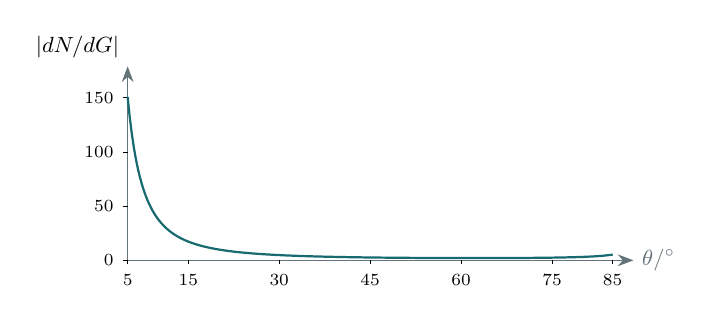
\begin{tikzpicture}[scale=.88,transform shape]
\draw[axis] (0,0.0)--(7.3,0.0) node[right] {$\theta/{}^\circ$};
\draw[axis] (0,0)--(0,2.8);
\node[above left] at (0,2.8) {$|dN/dG|$};
\draw[thin] (0.000000,0.0)--(0.000000,-0.06);\node[below,font=\scriptsize] at (0.000000,-0.08) {$ 5 $};
\draw[thin] (0.875000,0.0)--(0.875000,-0.06);\node[below,font=\scriptsize] at (0.875000,-0.08) {$ 15 $};
\draw[thin] (2.187500,0.0)--(2.187500,-0.06);\node[below,font=\scriptsize] at (2.187500,-0.08) {$ 30 $};
\draw[thin] (3.500000,0.0)--(3.500000,-0.06);\node[below,font=\scriptsize] at (3.500000,-0.08) {$ 45 $};
\draw[thin] (4.812500,0.0)--(4.812500,-0.06);\node[below,font=\scriptsize] at (4.812500,-0.08) {$ 60 $};
\draw[thin] (6.125000,0.0)--(6.125000,-0.06);\node[below,font=\scriptsize] at (6.125000,-0.08) {$ 75 $};
\draw[thin] (7.000000,0.0)--(7.000000,-0.06);\node[below,font=\scriptsize] at (7.000000,-0.08) {$ 85 $};
\draw[thin] (0,0.000000)--(-.06,0.000000);\node[left,font=\scriptsize] at (-.08,0.000000) {$ 0 $};
\draw[thin] (0,0.781250)--(-.06,0.781250);\node[left,font=\scriptsize] at (-.08,0.781250) {$ 50 $};
\draw[thin] (0,1.562500)--(-.06,1.562500);\node[left,font=\scriptsize] at (-.08,1.562500) {$ 100 $};
\draw[thin] (0,2.343750)--(-.06,2.343750);\node[left,font=\scriptsize] at (-.08,2.343750) {$ 150 $};
\draw[thick,color=accent] plot coordinates {(0.0000000,2.3584332) (0.0291667,2.0739566) (0.0583333,1.8381904) (0.0875000,1.6406169) (0.1166667,1.4734114) (0.1458333,1.3306550) (0.1750000,1.2078036) (0.2041667,1.1013218) (0.2333333,1.0084256) (0.2625000,0.9268988) (0.2916667,0.8549590) (0.3208333,0.7911603) (0.3500000,0.7343191) (0.3791667,0.6834597) (0.4083333,0.6377712) (0.4375000,0.5965761) (0.4666667,0.5593039) (0.4958333,0.5254720) (0.5250000,0.4946700) (0.5541667,0.4665466) (0.5833333,0.4408002) (0.6125000,0.4171704) (0.6416667,0.3954315) (0.6708333,0.3753872) (0.7000000,0.3568660) (0.7291667,0.3397174) (0.7583333,0.3238093) (0.7875000,0.3090249) (0.8166667,0.2952610) (0.8458333,0.2824259) (0.8750000,0.2704380) (0.9041667,0.2592245) (0.9333333,0.2487201) (0.9625000,0.2388665) (0.9916667,0.2296110) (1.0208333,0.2209064) (1.0500000,0.2127098) (1.0791667,0.2049827) (1.1083333,0.1976899) (1.1375000,0.1907996) (1.1666667,0.1842828) (1.1958333,0.1781131) (1.2250000,0.1722664) (1.2541667,0.1667206) (1.2833333,0.1614555) (1.3125000,0.1564526) (1.3416667,0.1516949) (1.3708333,0.1471667) (1.4000000,0.1428535) (1.4291667,0.1387421) (1.4583333,0.1348202) (1.4875000,0.1310763) (1.5166667,0.1275001) (1.5458333,0.1240816) (1.5750000,0.1208118) (1.6041667,0.1176824) (1.6333333,0.1146855) (1.6625000,0.1118138) (1.6916667,0.1090605) (1.7208333,0.1064193) (1.7500000,0.1038843) (1.7791667,0.1014500) (1.8083333,0.0991111) (1.8375000,0.0968629) (1.8666667,0.0947008) (1.8958333,0.0926205) (1.9250000,0.0906181) (1.9541667,0.0886898) (1.9833333,0.0868321) (2.0125000,0.0850417) (2.0416667,0.0833154) (2.0708333,0.0816503) (2.1000000,0.0800437) (2.1291667,0.0784928) (2.1583333,0.0769954) (2.1875000,0.0755489) (2.2166667,0.0741512) (2.2458333,0.0728003) (2.2750000,0.0714942) (2.3041667,0.0702309) (2.3333333,0.0690087) (2.3625000,0.0678260) (2.3916667,0.0666812) (2.4208333,0.0655726) (2.4500000,0.0644990) (2.4791667,0.0634590) (2.5083333,0.0624512) (2.5375000,0.0614744) (2.5666667,0.0605275) (2.5958333,0.0596093) (2.6250000,0.0587188) (2.6541667,0.0578550) (2.6833333,0.0570168) (2.7125000,0.0562035) (2.7416667,0.0554141) (2.7708333,0.0546478) (2.8000000,0.0539037) (2.8291667,0.0531812) (2.8583333,0.0524795) (2.8875000,0.0517979) (2.9166667,0.0511357) (2.9458333,0.0504924) (2.9750000,0.0498672) (3.0041667,0.0492597) (3.0333333,0.0486692) (3.0625000,0.0480953) (3.0916667,0.0475374) (3.1208333,0.0469951) (3.1500000,0.0464679) (3.1791667,0.0459552) (3.2083333,0.0454568) (3.2375000,0.0449722) (3.2666667,0.0445010) (3.2958333,0.0440428) (3.3250000,0.0435972) (3.3541667,0.0431640) (3.3833333,0.0427428) (3.4125000,0.0423333) (3.4416667,0.0419351) (3.4708333,0.0415479) (3.5000000,0.0411716) (3.5291667,0.0408058) (3.5583333,0.0404503) (3.5875000,0.0401047) (3.6166667,0.0397690) (3.6458333,0.0394428) (3.6750000,0.0391259) (3.7041667,0.0388182) (3.7333333,0.0385194) (3.7625000,0.0382293) (3.7916667,0.0379478) (3.8208333,0.0376746) (3.8500000,0.0374097) (3.8791667,0.0371528) (3.9083333,0.0369038) (3.9375000,0.0366625) (3.9666667,0.0364288) (3.9958333,0.0362026) (4.0250000,0.0359838) (4.0541667,0.0357722) (4.0833333,0.0355677) (4.1125000,0.0353702) (4.1416667,0.0351796) (4.1708333,0.0349958) (4.2000000,0.0348187) (4.2291667,0.0346482) (4.2583333,0.0344843) (4.2875000,0.0343268) (4.3166667,0.0341758) (4.3458333,0.0340311) (4.3750000,0.0338926) (4.4041667,0.0337604) (4.4333333,0.0336344) (4.4625000,0.0335145) (4.4916667,0.0334006) (4.5208333,0.0332929) (4.5500000,0.0331911) (4.5791667,0.0330954) (4.6083333,0.0330056) (4.6375000,0.0329219) (4.6666667,0.0328440) (4.6958333,0.0327722) (4.7250000,0.0327063) (4.7541667,0.0326463) (4.7833333,0.0325924) (4.8125000,0.0325444) (4.8416667,0.0325025) (4.8708333,0.0324666) (4.9000000,0.0324369) (4.9291667,0.0324132) (4.9583333,0.0323958) (4.9875000,0.0323846) (5.0166667,0.0323797) (5.0458333,0.0323812) (5.0750000,0.0323892) (5.1041667,0.0324037) (5.1333333,0.0324248) (5.1625000,0.0324527) (5.1916667,0.0324875) (5.2208333,0.0325293) (5.2500000,0.0325782) (5.2791667,0.0326344) (5.3083333,0.0326980) (5.3375000,0.0327692) (5.3666667,0.0328481) (5.3958333,0.0329351) (5.4250000,0.0330302) (5.4541667,0.0331338) (5.4833333,0.0332460) (5.5125000,0.0333671) (5.5416667,0.0334975) (5.5708333,0.0336373) (5.6000000,0.0337870) (5.6291667,0.0339468) (5.6583333,0.0341172) (5.6875000,0.0342985) (5.7166667,0.0344913) (5.7458333,0.0346958) (5.7750000,0.0349127) (5.8041667,0.0351425) (5.8333333,0.0353857) (5.8625000,0.0356430) (5.8916667,0.0359151) (5.9208333,0.0362026) (5.9500000,0.0365065) (5.9791667,0.0368274) (6.0083333,0.0371665) (6.0375000,0.0375245) (6.0666667,0.0379028) (6.0958333,0.0383024) (6.1250000,0.0387246) (6.1541667,0.0391709) (6.1833333,0.0396429) (6.2125000,0.0401422) (6.2416667,0.0406707) (6.2708333,0.0412305) (6.3000000,0.0418239) (6.3291667,0.0424534) (6.3583333,0.0431217) (6.3875000,0.0438321) (6.4166667,0.0445880) (6.4458333,0.0453932) (6.4750000,0.0462522) (6.5041667,0.0471698) (6.5333333,0.0481515) (6.5625000,0.0492038) (6.5916667,0.0503336) (6.6208333,0.0515492) (6.6500000,0.0528600) (6.6791667,0.0542768) (6.7083333,0.0558122) (6.7375000,0.0574808) (6.7666667,0.0593000) (6.7958333,0.0612899) (6.8250000,0.0634750) (6.8541667,0.0658843) (6.8833333,0.0685530) (6.9125000,0.0715242) (6.9416667,0.0748511) (6.9708333,0.0786002) (7.0000000,0.0828557)};
\end{tikzpicture}
\figcaption{解图光4.9D\quad 固定绝对复比误差在近法向被明显放大}
\end{minipage}\end{center}


\Needspace{13\baselineskip}

\pdfbookmark[2]{第 10 题 石英棱镜的双折射分离}{q10}

\section*{第 10 题\quad 石英棱镜的双折射分离}\label{q:10}

顶角$A=60^\circ$的石英棱镜，其光轴垂直主截面。在钠黄光处主折射率为$n_o=1.544,n_e=1.553$。同一束自然平行光从空气入射，取入射角为两主折射率各自最小偏向入射角的平均值。两出射束由焦距$f=1.00\,\mathrm m$的薄透镜聚焦，透镜轴取两出射方向的中线。求两焦点间距，并解释最小偏向条件在本题中的使用。

\begin{center}\begin{minipage}{.98\linewidth}\centering
\begin{tikzpicture}[scale=.8,transform shape]
\draw[object] (-1.50111,0.00000)--(0.00000,2.60000)--(1.50111,0.00000)--(-1.50111,0.00000);\draw[motion] (-2.65747,0.78178)--(-0.60000,1.56077);\node[above left] at (-2.65747,0.78178) {共同入射};\draw[motion] (-0.60000,1.56077)--(0.59883,1.56279);
\draw[motion] (0.59883,1.56279)--(3.41194,0.52047);\draw[force] (-0.60000,1.56077)--(0.60116,1.55877);
\draw[force] (0.60116,1.55877)--(3.39916,0.47655);\node[above] at (0.00000,2.80000) {$A$};\node[below] at (0.20000,-0.30000) {同一入射方向};\node[above] at (3.50000,1.20000) {两路径按Snell关系计算};
\end{tikzpicture}
\figcaption{图光4.10\quad 同一入射束经过双折射棱镜}
\end{minipage}\end{center}

\Needspace{6\baselineskip}\subsection*{解答}


图光4.10的波矢在棱镜主截面内，晶体光轴垂直这个截面，故每一内部方向都与光轴成$90^\circ$。在此几何中$o,e$的有效折射率分别为常数$n_o,n_e$；$e$波的能流也沿波法线，逐面折射可以直接使用这两个折射率。两折射率共用同一个入射方向，入口和出口的角度均按各自面的法线量取。

对任一折射率$n$，最小偏向时$r_1=r_2=A/2$，入射角为
\[
i_{\min}(n)=\arcsin\left(n\sin\frac A2\right).
\]
分别代入两主折射率，有$i_{\min,o}=50.5338284^\circ$、$i_{\min,e}=50.9412264^\circ$。题设采用它们的平均值：
\[
i=\frac{i_{\min}(n_o)+i_{\min}(n_e)}2=50.7375274^\circ.
\]
此时两束分别位于各自最小偏向位置附近。解图光4.10A按共同输入、入口、出口列出计算顺序，焦平面上的两点由最后的实际方向差决定。
\begin{center}\begin{minipage}{.98\linewidth}\centering
\begin{tikzpicture}[scale=.78,transform shape]
\node[above right] at (0.00000,0.40000) {步骤};\node[above right] at (2.50000,0.40000) {分量或关系};\node[above right] at (9.20000,0.40000) {说明};\draw[thin] (-0.20000,0.10000)--(12.60000,0.10000);\node[above right] at (0.00000,-0.48000) {共同入射};\node[above right] at (2.50000,-0.48000) {$i=50.737527^\circ$};\node[above right] at (9.20000,-0.48000) {两束同一方向};\node[above right] at (0.00000,-1.11000) {入口};\node[above right] at (2.50000,-1.11000) {$r_{1j}=\arcsin(\sin i/n_j)$};\node[above right] at (9.20000,-1.11000) {先发生分裂};\node[above right] at (0.00000,-1.74000) {出口};\node[above right] at (2.50000,-1.74000) {$\beta_j=\arcsin[n_j\sin(A-r_{1j})]$};\node[above right] at (9.20000,-1.74000) {再发生分裂};\begin{scope}[shift={(3.00000,-4.10000)}]
\draw[motion] (0.00000,0.00000)--(3.00000,1.10000);\draw[force] (0.00000,0.00000)--(3.00000,-1.10000);\draw[object] (3.00000,-1.60000)--(3.00000,1.60000);\fill (3.00000,1.10000) circle(.035);\node[right] at (3.00000,1.10000) {$P_o$};\fill (3.00000,-1.10000) circle(.035);\node[right] at (3.00000,-1.10000) {$P_e$};\draw[<->,thin,color=muted] (4.00000,-1.10000)--(4.00000,1.10000);\node[right] at (4.00000,0.00000) {$\Delta x$};\node[below] at (1.30000,-1.70000) {角分离放大示意};\node[above] at (1.40000,1.80000) {透镜轴：出射中线};
\end{scope}
\end{tikzpicture}
\figcaption{解图光4.10A\quad 两个界面的分裂与后焦面间距}
\end{minipage}\end{center}
沿图光4.10中的两条内部路径，对$j=o,e$依次应用Snell关系和棱镜几何：
\[
r_{1j}=\arcsin\frac{\sin i}{n_j},\qquad
r_{2j}=A-r_{1j},\qquad
\beta_j=\arcsin(n_j\sin r_{2j}).
\]
具体角度为
\[
 \begin{array}{c|ccc}
 j&r_{1j}&r_{2j}&\beta_j\\\hline
 o&30.09666794^\circ&29.90333206^\circ&50.33080795^\circ\\
 e&29.90440204^\circ&30.09559796^\circ&51.14562431^\circ
 \end{array}
\]
入口的不同折射率使内部方向已经分开：$r_{1e}<r_{1o}$，故第二面的内部入射角$r_{2e}>r_{2o}$；出口的两种折射作用与这一内部角差共同决定分离。解图光4.10B把两出射角作为共同入射角的函数；在同一入射角处读取两曲线的纵坐标，便得到实际分离。
\begin{center}\begin{minipage}{.98\linewidth}\centering
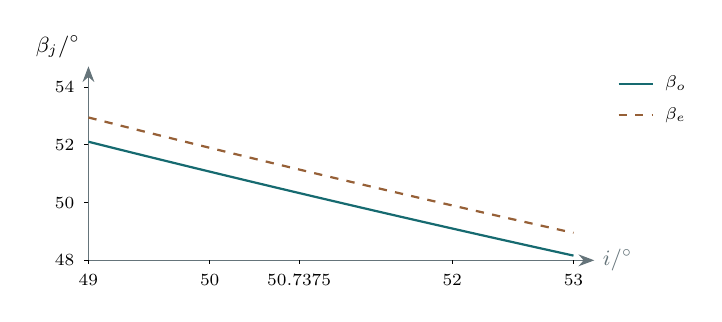
\begin{tikzpicture}[scale=.88,transform shape]
\draw[axis] (0,0)--(7.3,0) node[right] {$i/{}^\circ$};
\draw[axis] (0,0)--(0,2.8);
\node[above left] at (0,2.8) {$\beta_j/{}^\circ$};
\draw[thin] (0.000000,0)--(0.000000,-0.06);\node[below,font=\scriptsize] at (0.000000,-0.08) {$ 49 $};
\draw[thin] (1.750000,0)--(1.750000,-0.06);\node[below,font=\scriptsize] at (1.750000,-0.08) {$ 50 $};
\draw[thin] (3.040672,0)--(3.040672,-0.06);\node[below,font=\scriptsize] at (3.040672,-0.08) {$ 50.7375 $};
\draw[thin] (5.250000,0)--(5.250000,-0.06);\node[below,font=\scriptsize] at (5.250000,-0.08) {$ 52 $};
\draw[thin] (7.000000,0)--(7.000000,-0.06);\node[below,font=\scriptsize] at (7.000000,-0.08) {$ 53 $};
\draw[thin] (0,0.000000)--(-.06,0.000000);\node[left,font=\scriptsize] at (-.08,0.000000) {$ 48 $};
\draw[thin] (0,0.833333)--(-.06,0.833333);\node[left,font=\scriptsize] at (-.08,0.833333) {$ 50 $};
\draw[thin] (0,1.666667)--(-.06,1.666667);\node[left,font=\scriptsize] at (-.08,1.666667) {$ 52 $};
\draw[thin] (0,2.500000)--(-.06,2.500000);\node[left,font=\scriptsize] at (-.08,2.500000) {$ 54 $};
\draw[thick,color=accent] plot coordinates {(0.0000000,1.7113727) (0.0291667,1.7040664) (0.0583333,1.6967642) (0.0875000,1.6894662) (0.1166667,1.6821722) (0.1458333,1.6748824) (0.1750000,1.6675966) (0.2041667,1.6603150) (0.2333333,1.6530374) (0.2625000,1.6457640) (0.2916667,1.6384946) (0.3208333,1.6312294) (0.3500000,1.6239682) (0.3791667,1.6167110) (0.4083333,1.6094580) (0.4375000,1.6022090) (0.4666667,1.5949641) (0.4958333,1.5877232) (0.5250000,1.5804865) (0.5541667,1.5732537) (0.5833333,1.5660250) (0.6125000,1.5588004) (0.6416667,1.5515798) (0.6708333,1.5443632) (0.7000000,1.5371507) (0.7291667,1.5299422) (0.7583333,1.5227377) (0.7875000,1.5155373) (0.8166667,1.5083409) (0.8458333,1.5011485) (0.8750000,1.4939601) (0.9041667,1.4867757) (0.9333333,1.4795953) (0.9625000,1.4724189) (0.9916667,1.4652465) (1.0208333,1.4580781) (1.0500000,1.4509137) (1.0791667,1.4437533) (1.1083333,1.4365969) (1.1375000,1.4294445) (1.1666667,1.4222960) (1.1958333,1.4151515) (1.2250000,1.4080110) (1.2541667,1.4008744) (1.2833333,1.3937418) (1.3125000,1.3866131) (1.3416667,1.3794884) (1.3708333,1.3723677) (1.4000000,1.3652509) (1.4291667,1.3581381) (1.4583333,1.3510292) (1.4875000,1.3439242) (1.5166667,1.3368231) (1.5458333,1.3297260) (1.5750000,1.3226329) (1.6041667,1.3155436) (1.6333333,1.3084583) (1.6625000,1.3013768) (1.6916667,1.2942993) (1.7208333,1.2872257) (1.7500000,1.2801560) (1.7791667,1.2730902) (1.8083333,1.2660283) (1.8375000,1.2589703) (1.8666667,1.2519162) (1.8958333,1.2448660) (1.9250000,1.2378197) (1.9541667,1.2307772) (1.9833333,1.2237387) (2.0125000,1.2167040) (2.0416667,1.2096731) (2.0708333,1.2026462) (2.1000000,1.1956231) (2.1291667,1.1886039) (2.1583333,1.1815885) (2.1875000,1.1745770) (2.2166667,1.1675693) (2.2458333,1.1605655) (2.2750000,1.1535656) (2.3041667,1.1465694) (2.3333333,1.1395772) (2.3625000,1.1325887) (2.3916667,1.1256041) (2.4208333,1.1186233) (2.4500000,1.1116464) (2.4791667,1.1046732) (2.5083333,1.0977039) (2.5375000,1.0907384) (2.5666667,1.0837767) (2.5958333,1.0768189) (2.6250000,1.0698648) (2.6541667,1.0629146) (2.6833333,1.0559681) (2.7125000,1.0490254) (2.7416667,1.0420866) (2.7708333,1.0351515) (2.8000000,1.0282202) (2.8291667,1.0212927) (2.8583333,1.0143690) (2.8875000,1.0074491) (2.9166667,1.0005329) (2.9458333,0.9936205) (2.9750000,0.9867119) (3.0041667,0.9798071) (3.0333333,0.9729060) (3.0625000,0.9660087) (3.0916667,0.9591151) (3.1208333,0.9522253) (3.1500000,0.9453392) (3.1791667,0.9384569) (3.2083333,0.9315784) (3.2375000,0.9247036) (3.2666667,0.9178325) (3.2958333,0.9109652) (3.3250000,0.9041016) (3.3541667,0.8972417) (3.3833333,0.8903855) (3.4125000,0.8835331) (3.4416667,0.8766844) (3.4708333,0.8698395) (3.5000000,0.8629982) (3.5291667,0.8561607) (3.5583333,0.8493268) (3.5875000,0.8424967) (3.6166667,0.8356703) (3.6458333,0.8288476) (3.6750000,0.8220286) (3.7041667,0.8152133) (3.7333333,0.8084016) (3.7625000,0.8015937) (3.7916667,0.7947895) (3.8208333,0.7879889) (3.8500000,0.7811920) (3.8791667,0.7743988) (3.9083333,0.7676093) (3.9375000,0.7608235) (3.9666667,0.7540413) (3.9958333,0.7472628) (4.0250000,0.7404880) (4.0541667,0.7337168) (4.0833333,0.7269493) (4.1125000,0.7201854) (4.1416667,0.7134253) (4.1708333,0.7066687) (4.2000000,0.6999158) (4.2291667,0.6931666) (4.2583333,0.6864210) (4.2875000,0.6796790) (4.3166667,0.6729407) (4.3458333,0.6662060) (4.3750000,0.6594749) (4.4041667,0.6527475) (4.4333333,0.6460237) (4.4625000,0.6393036) (4.4916667,0.6325870) (4.5208333,0.6258741) (4.5500000,0.6191648) (4.5791667,0.6124591) (4.6083333,0.6057570) (4.6375000,0.5990585) (4.6666667,0.5923637) (4.6958333,0.5856724) (4.7250000,0.5789848) (4.7541667,0.5723007) (4.7833333,0.5656202) (4.8125000,0.5589434) (4.8416667,0.5522701) (4.8708333,0.5456004) (4.9000000,0.5389343) (4.9291667,0.5322718) (4.9583333,0.5256129) (4.9875000,0.5189575) (5.0166667,0.5123058) (5.0458333,0.5056576) (5.0750000,0.4990129) (5.1041667,0.4923719) (5.1333333,0.4857344) (5.1625000,0.4791004) (5.1916667,0.4724701) (5.2208333,0.4658433) (5.2500000,0.4592200) (5.2791667,0.4526003) (5.3083333,0.4459842) (5.3375000,0.4393716) (5.3666667,0.4327625) (5.3958333,0.4261570) (5.4250000,0.4195550) (5.4541667,0.4129566) (5.4833333,0.4063617) (5.5125000,0.3997704) (5.5416667,0.3931826) (5.5708333,0.3865983) (5.6000000,0.3800175) (5.6291667,0.3734403) (5.6583333,0.3668665) (5.6875000,0.3602964) (5.7166667,0.3537297) (5.7458333,0.3471665) (5.7750000,0.3406069) (5.8041667,0.3340507) (5.8333333,0.3274981) (5.8625000,0.3209490) (5.8916667,0.3144034) (5.9208333,0.3078612) (5.9500000,0.3013226) (5.9791667,0.2947875) (6.0083333,0.2882559) (6.0375000,0.2817277) (6.0666667,0.2752031) (6.0958333,0.2686819) (6.1250000,0.2621643) (6.1541667,0.2556501) (6.1833333,0.2491394) (6.2125000,0.2426321) (6.2416667,0.2361284) (6.2708333,0.2296281) (6.3000000,0.2231313) (6.3291667,0.2166380) (6.3583333,0.2101481) (6.3875000,0.2036617) (6.4166667,0.1971788) (6.4458333,0.1906993) (6.4750000,0.1842233) (6.5041667,0.1777507) (6.5333333,0.1712816) (6.5625000,0.1648159) (6.5916667,0.1583537) (6.6208333,0.1518950) (6.6500000,0.1454397) (6.6791667,0.1389878) (6.7083333,0.1325394) (6.7375000,0.1260944) (6.7666667,0.1196528) (6.7958333,0.1132147) (6.8250000,0.1067800) (6.8541667,0.1003488) (6.8833333,0.0939209) (6.9125000,0.0874965) (6.9416667,0.0810756) (6.9708333,0.0746580) (7.0000000,0.0682439)};
\draw[thick,color=accent] (7.65,2.55)--(8.15,2.55);\node[right,font=\scriptsize] at (8.2,2.55) {$\beta_o$};
\draw[thick,dashed,color=warm] plot coordinates {(0.0000000,2.0616457) (0.0291667,2.0542261) (0.0583333,2.0468108) (0.0875000,2.0393999) (0.1166667,2.0319933) (0.1458333,2.0245910) (0.1750000,2.0171931) (0.2041667,2.0097994) (0.2333333,2.0024101) (0.2625000,1.9950250) (0.2916667,1.9876442) (0.3208333,1.9802677) (0.3500000,1.9728955) (0.3791667,1.9655276) (0.4083333,1.9581640) (0.4375000,1.9508046) (0.4666667,1.9434495) (0.4958333,1.9360987) (0.5250000,1.9287521) (0.5541667,1.9214098) (0.5833333,1.9140718) (0.6125000,1.9067379) (0.6416667,1.8994084) (0.6708333,1.8920830) (0.7000000,1.8847619) (0.7291667,1.8774450) (0.7583333,1.8701324) (0.7875000,1.8628239) (0.8166667,1.8555197) (0.8458333,1.8482197) (0.8750000,1.8409239) (0.9041667,1.8336324) (0.9333333,1.8263450) (0.9625000,1.8190618) (0.9916667,1.8117828) (1.0208333,1.8045080) (1.0500000,1.7972373) (1.0791667,1.7899709) (1.1083333,1.7827086) (1.1375000,1.7754505) (1.1666667,1.7681966) (1.1958333,1.7609468) (1.2250000,1.7537012) (1.2541667,1.7464597) (1.2833333,1.7392224) (1.3125000,1.7319893) (1.3416667,1.7247603) (1.3708333,1.7175354) (1.4000000,1.7103147) (1.4291667,1.7030981) (1.4583333,1.6958856) (1.4875000,1.6886772) (1.5166667,1.6814730) (1.5458333,1.6742729) (1.5750000,1.6670769) (1.6041667,1.6598850) (1.6333333,1.6526972) (1.6625000,1.6455135) (1.6916667,1.6383339) (1.7208333,1.6311584) (1.7500000,1.6239870) (1.7791667,1.6168196) (1.8083333,1.6096564) (1.8375000,1.6024972) (1.8666667,1.5953421) (1.8958333,1.5881911) (1.9250000,1.5810441) (1.9541667,1.5739012) (1.9833333,1.5667624) (2.0125000,1.5596276) (2.0416667,1.5524969) (2.0708333,1.5453702) (2.1000000,1.5382475) (2.1291667,1.5311289) (2.1583333,1.5240144) (2.1875000,1.5169038) (2.2166667,1.5097973) (2.2458333,1.5026948) (2.2750000,1.4955964) (2.3041667,1.4885019) (2.3333333,1.4814115) (2.3625000,1.4743251) (2.3916667,1.4672427) (2.4208333,1.4601643) (2.4500000,1.4530899) (2.4791667,1.4460195) (2.5083333,1.4389531) (2.5375000,1.4318906) (2.5666667,1.4248322) (2.5958333,1.4177778) (2.6250000,1.4107273) (2.6541667,1.4036808) (2.6833333,1.3966382) (2.7125000,1.3895997) (2.7416667,1.3825651) (2.7708333,1.3755345) (2.8000000,1.3685078) (2.8291667,1.3614851) (2.8583333,1.3544663) (2.8875000,1.3474515) (2.9166667,1.3404406) (2.9458333,1.3334337) (2.9750000,1.3264307) (3.0041667,1.3194316) (3.0333333,1.3124364) (3.0625000,1.3054452) (3.0916667,1.2984580) (3.1208333,1.2914746) (3.1500000,1.2844951) (3.1791667,1.2775196) (3.2083333,1.2705480) (3.2375000,1.2635803) (3.2666667,1.2566165) (3.2958333,1.2496566) (3.3250000,1.2427005) (3.3541667,1.2357484) (3.3833333,1.2288002) (3.4125000,1.2218558) (3.4416667,1.2149154) (3.4708333,1.2079788) (3.5000000,1.2010461) (3.5291667,1.1941173) (3.5583333,1.1871923) (3.5875000,1.1802712) (3.6166667,1.1733540) (3.6458333,1.1664407) (3.6750000,1.1595312) (3.7041667,1.1526255) (3.7333333,1.1457237) (3.7625000,1.1388258) (3.7916667,1.1319317) (3.8208333,1.1250414) (3.8500000,1.1181550) (3.8791667,1.1112724) (3.9083333,1.1043937) (3.9375000,1.0975188) (3.9666667,1.0906477) (3.9958333,1.0837804) (4.0250000,1.0769170) (4.0541667,1.0700573) (4.0833333,1.0632015) (4.1125000,1.0563495) (4.1416667,1.0495013) (4.1708333,1.0426569) (4.2000000,1.0358163) (4.2291667,1.0289796) (4.2583333,1.0221466) (4.2875000,1.0153174) (4.3166667,1.0084920) (4.3458333,1.0016703) (4.3750000,0.9948525) (4.4041667,0.9880384) (4.4333333,0.9812282) (4.4625000,0.9744217) (4.4916667,0.9676189) (4.5208333,0.9608200) (4.5500000,0.9540248) (4.5791667,0.9472334) (4.6083333,0.9404457) (4.6375000,0.9336618) (4.6666667,0.9268816) (4.6958333,0.9201052) (4.7250000,0.9133326) (4.7541667,0.9065637) (4.7833333,0.8997985) (4.8125000,0.8930371) (4.8416667,0.8862794) (4.8708333,0.8795254) (4.9000000,0.8727752) (4.9291667,0.8660287) (4.9583333,0.8592860) (4.9875000,0.8525469) (5.0166667,0.8458116) (5.0458333,0.8390800) (5.0750000,0.8323521) (5.1041667,0.8256279) (5.1333333,0.8189075) (5.1625000,0.8121907) (5.1916667,0.8054776) (5.2208333,0.7987683) (5.2500000,0.7920626) (5.2791667,0.7853607) (5.3083333,0.7786624) (5.3375000,0.7719678) (5.3666667,0.7652769) (5.3958333,0.7585897) (5.4250000,0.7519062) (5.4541667,0.7452264) (5.4833333,0.7385502) (5.5125000,0.7318777) (5.5416667,0.7252089) (5.5708333,0.7185437) (5.6000000,0.7118822) (5.6291667,0.7052244) (5.6583333,0.6985702) (5.6875000,0.6919197) (5.7166667,0.6852729) (5.7458333,0.6786297) (5.7750000,0.6719901) (5.8041667,0.6653542) (5.8333333,0.6587220) (5.8625000,0.6520933) (5.8916667,0.6454684) (5.9208333,0.6388470) (5.9500000,0.6322293) (5.9791667,0.6256152) (6.0083333,0.6190048) (6.0375000,0.6123980) (6.0666667,0.6057948) (6.0958333,0.5991952) (6.1250000,0.5925992) (6.1541667,0.5860069) (6.1833333,0.5794182) (6.2125000,0.5728331) (6.2416667,0.5662516) (6.2708333,0.5596737) (6.3000000,0.5530994) (6.3291667,0.5465287) (6.3583333,0.5399616) (6.3875000,0.5333981) (6.4166667,0.5268382) (6.4458333,0.5202819) (6.4750000,0.5137292) (6.5041667,0.5071800) (6.5333333,0.5006345) (6.5625000,0.4940925) (6.5916667,0.4875541) (6.6208333,0.4810193) (6.6500000,0.4744880) (6.6791667,0.4679604) (6.7083333,0.4614363) (6.7375000,0.4549157) (6.7666667,0.4483988) (6.7958333,0.4418854) (6.8250000,0.4353755) (6.8541667,0.4288692) (6.8833333,0.4223665) (6.9125000,0.4158673) (6.9416667,0.4093717) (6.9708333,0.4028796) (7.0000000,0.3963911)};
\draw[thick,dashed,color=warm] (7.65,2.0999999999999996)--(8.15,2.0999999999999996);\node[right,font=\scriptsize] at (8.2,2.0999999999999996) {$\beta_e$};
\end{tikzpicture}
\figcaption{解图光4.10B\quad 两出射角的差在同一共同入射角处读取}
\end{minipage}\end{center}
由上表$\Delta\beta=\beta_e-\beta_o=0.81481636^\circ=0.0142212283\,\mathrm{rad}$。透镜轴取两出射方向的中线，各束与轴的夹角为$\mp\Delta\beta/2$。后焦面上分别有$x_o=-f\tan(\Delta\beta/2)$、$x_e=f\tan(\Delta\beta/2)$，所以
\[
\boxed{\Delta x=2f\tan\frac{\Delta\beta}{2}
=14.2215\,\mathrm{mm}}.
\]
近轴形式$f\Delta\beta$给$14.2212\,\mathrm{mm}$，与正切形式仅差约$0.00024\,\mathrm{mm}$。解图光4.10C的两支焦点位置随焦距成比例，$f=1\,\mathrm m$时分别为$\pm7.110734\,\mathrm{mm}$。
\begin{center}\begin{minipage}{.98\linewidth}\centering
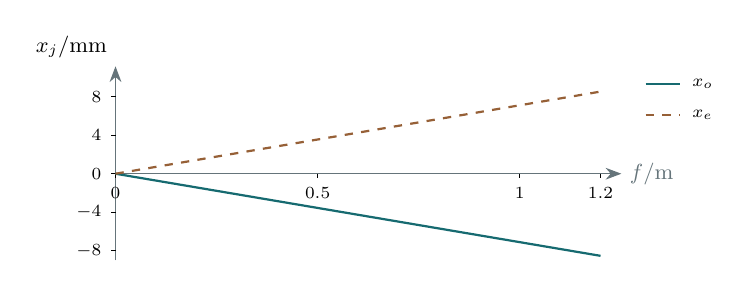
\begin{tikzpicture}[scale=.88,transform shape]
\draw[axis] (0,1.25)--(7.3,1.25) node[right] {$f/{\rm m}$};
\draw[axis] (0,0)--(0,2.8);
\node[above left] at (0,2.8) {$x_j/{\rm mm}$};
\draw[thin] (0.000000,1.25)--(0.000000,1.19);\node[below,font=\scriptsize] at (0.000000,1.17) {$ 0 $};
\draw[thin] (2.916667,1.25)--(2.916667,1.19);\node[below,font=\scriptsize] at (2.916667,1.17) {$ 0.5 $};
\draw[thin] (5.833333,1.25)--(5.833333,1.19);\node[below,font=\scriptsize] at (5.833333,1.17) {$ 1 $};
\draw[thin] (7.000000,1.25)--(7.000000,1.19);\node[below,font=\scriptsize] at (7.000000,1.17) {$ 1.2 $};
\draw[thin] (0,0.138889)--(-.06,0.138889);\node[left,font=\scriptsize] at (-.08,0.138889) {$ -8 $};
\draw[thin] (0,0.694444)--(-.06,0.694444);\node[left,font=\scriptsize] at (-.08,0.694444) {$ -4 $};
\draw[thin] (0,1.250000)--(-.06,1.250000);\node[left,font=\scriptsize] at (-.08,1.250000) {$ 0 $};
\draw[thin] (0,1.805556)--(-.06,1.805556);\node[left,font=\scriptsize] at (-.08,1.805556) {$ 4 $};
\draw[thin] (0,2.361111)--(-.06,2.361111);\node[left,font=\scriptsize] at (-.08,2.361111) {$ 8 $};
\draw[thick,color=accent] plot coordinates {(0.0000000,1.2500000) (0.0291667,1.2450620) (0.0583333,1.2401240) (0.0875000,1.2351860) (0.1166667,1.2302480) (0.1458333,1.2253100) (0.1750000,1.2203719) (0.2041667,1.2154339) (0.2333333,1.2104959) (0.2625000,1.2055579) (0.2916667,1.2006199) (0.3208333,1.1956819) (0.3500000,1.1907439) (0.3791667,1.1858059) (0.4083333,1.1808679) (0.4375000,1.1759299) (0.4666667,1.1709918) (0.4958333,1.1660538) (0.5250000,1.1611158) (0.5541667,1.1561778) (0.5833333,1.1512398) (0.6125000,1.1463018) (0.6416667,1.1413638) (0.6708333,1.1364258) (0.7000000,1.1314878) (0.7291667,1.1265498) (0.7583333,1.1216117) (0.7875000,1.1166737) (0.8166667,1.1117357) (0.8458333,1.1067977) (0.8750000,1.1018597) (0.9041667,1.0969217) (0.9333333,1.0919837) (0.9625000,1.0870457) (0.9916667,1.0821077) (1.0208333,1.0771697) (1.0500000,1.0722317) (1.0791667,1.0672936) (1.1083333,1.0623556) (1.1375000,1.0574176) (1.1666667,1.0524796) (1.1958333,1.0475416) (1.2250000,1.0426036) (1.2541667,1.0376656) (1.2833333,1.0327276) (1.3125000,1.0277896) (1.3416667,1.0228516) (1.3708333,1.0179135) (1.4000000,1.0129755) (1.4291667,1.0080375) (1.4583333,1.0030995) (1.4875000,0.9981615) (1.5166667,0.9932235) (1.5458333,0.9882855) (1.5750000,0.9833475) (1.6041667,0.9784095) (1.6333333,0.9734715) (1.6625000,0.9685334) (1.6916667,0.9635954) (1.7208333,0.9586574) (1.7500000,0.9537194) (1.7791667,0.9487814) (1.8083333,0.9438434) (1.8375000,0.9389054) (1.8666667,0.9339674) (1.8958333,0.9290294) (1.9250000,0.9240914) (1.9541667,0.9191533) (1.9833333,0.9142153) (2.0125000,0.9092773) (2.0416667,0.9043393) (2.0708333,0.8994013) (2.1000000,0.8944633) (2.1291667,0.8895253) (2.1583333,0.8845873) (2.1875000,0.8796493) (2.2166667,0.8747113) (2.2458333,0.8697733) (2.2750000,0.8648352) (2.3041667,0.8598972) (2.3333333,0.8549592) (2.3625000,0.8500212) (2.3916667,0.8450832) (2.4208333,0.8401452) (2.4500000,0.8352072) (2.4791667,0.8302692) (2.5083333,0.8253312) (2.5375000,0.8203932) (2.5666667,0.8154551) (2.5958333,0.8105171) (2.6250000,0.8055791) (2.6541667,0.8006411) (2.6833333,0.7957031) (2.7125000,0.7907651) (2.7416667,0.7858271) (2.7708333,0.7808891) (2.8000000,0.7759511) (2.8291667,0.7710131) (2.8583333,0.7660750) (2.8875000,0.7611370) (2.9166667,0.7561990) (2.9458333,0.7512610) (2.9750000,0.7463230) (3.0041667,0.7413850) (3.0333333,0.7364470) (3.0625000,0.7315090) (3.0916667,0.7265710) (3.1208333,0.7216330) (3.1500000,0.7166950) (3.1791667,0.7117569) (3.2083333,0.7068189) (3.2375000,0.7018809) (3.2666667,0.6969429) (3.2958333,0.6920049) (3.3250000,0.6870669) (3.3541667,0.6821289) (3.3833333,0.6771909) (3.4125000,0.6722529) (3.4416667,0.6673149) (3.4708333,0.6623768) (3.5000000,0.6574388) (3.5291667,0.6525008) (3.5583333,0.6475628) (3.5875000,0.6426248) (3.6166667,0.6376868) (3.6458333,0.6327488) (3.6750000,0.6278108) (3.7041667,0.6228728) (3.7333333,0.6179348) (3.7625000,0.6129967) (3.7916667,0.6080587) (3.8208333,0.6031207) (3.8500000,0.5981827) (3.8791667,0.5932447) (3.9083333,0.5883067) (3.9375000,0.5833687) (3.9666667,0.5784307) (3.9958333,0.5734927) (4.0250000,0.5685547) (4.0541667,0.5636167) (4.0833333,0.5586786) (4.1125000,0.5537406) (4.1416667,0.5488026) (4.1708333,0.5438646) (4.2000000,0.5389266) (4.2291667,0.5339886) (4.2583333,0.5290506) (4.2875000,0.5241126) (4.3166667,0.5191746) (4.3458333,0.5142366) (4.3750000,0.5092985) (4.4041667,0.5043605) (4.4333333,0.4994225) (4.4625000,0.4944845) (4.4916667,0.4895465) (4.5208333,0.4846085) (4.5500000,0.4796705) (4.5791667,0.4747325) (4.6083333,0.4697945) (4.6375000,0.4648565) (4.6666667,0.4599184) (4.6958333,0.4549804) (4.7250000,0.4500424) (4.7541667,0.4451044) (4.7833333,0.4401664) (4.8125000,0.4352284) (4.8416667,0.4302904) (4.8708333,0.4253524) (4.9000000,0.4204144) (4.9291667,0.4154764) (4.9583333,0.4105383) (4.9875000,0.4056003) (5.0166667,0.4006623) (5.0458333,0.3957243) (5.0750000,0.3907863) (5.1041667,0.3858483) (5.1333333,0.3809103) (5.1625000,0.3759723) (5.1916667,0.3710343) (5.2208333,0.3660963) (5.2500000,0.3611583) (5.2791667,0.3562202) (5.3083333,0.3512822) (5.3375000,0.3463442) (5.3666667,0.3414062) (5.3958333,0.3364682) (5.4250000,0.3315302) (5.4541667,0.3265922) (5.4833333,0.3216542) (5.5125000,0.3167162) (5.5416667,0.3117782) (5.5708333,0.3068401) (5.6000000,0.3019021) (5.6291667,0.2969641) (5.6583333,0.2920261) (5.6875000,0.2870881) (5.7166667,0.2821501) (5.7458333,0.2772121) (5.7750000,0.2722741) (5.8041667,0.2673361) (5.8333333,0.2623981) (5.8625000,0.2574600) (5.8916667,0.2525220) (5.9208333,0.2475840) (5.9500000,0.2426460) (5.9791667,0.2377080) (6.0083333,0.2327700) (6.0375000,0.2278320) (6.0666667,0.2228940) (6.0958333,0.2179560) (6.1250000,0.2130180) (6.1541667,0.2080800) (6.1833333,0.2031419) (6.2125000,0.1982039) (6.2416667,0.1932659) (6.2708333,0.1883279) (6.3000000,0.1833899) (6.3291667,0.1784519) (6.3583333,0.1735139) (6.3875000,0.1685759) (6.4166667,0.1636379) (6.4458333,0.1586999) (6.4750000,0.1537618) (6.5041667,0.1488238) (6.5333333,0.1438858) (6.5625000,0.1389478) (6.5916667,0.1340098) (6.6208333,0.1290718) (6.6500000,0.1241338) (6.6791667,0.1191958) (6.7083333,0.1142578) (6.7375000,0.1093198) (6.7666667,0.1043817) (6.7958333,0.0994437) (6.8250000,0.0945057) (6.8541667,0.0895677) (6.8833333,0.0846297) (6.9125000,0.0796917) (6.9416667,0.0747537) (6.9708333,0.0698157) (7.0000000,0.0648777)};
\draw[thick,color=accent] (7.65,2.55)--(8.15,2.55);\node[right,font=\scriptsize] at (8.2,2.55) {$x_o$};
\draw[thick,dashed,color=warm] plot coordinates {(0.0000000,1.2500000) (0.0291667,1.2549380) (0.0583333,1.2598760) (0.0875000,1.2648140) (0.1166667,1.2697520) (0.1458333,1.2746900) (0.1750000,1.2796281) (0.2041667,1.2845661) (0.2333333,1.2895041) (0.2625000,1.2944421) (0.2916667,1.2993801) (0.3208333,1.3043181) (0.3500000,1.3092561) (0.3791667,1.3141941) (0.4083333,1.3191321) (0.4375000,1.3240701) (0.4666667,1.3290082) (0.4958333,1.3339462) (0.5250000,1.3388842) (0.5541667,1.3438222) (0.5833333,1.3487602) (0.6125000,1.3536982) (0.6416667,1.3586362) (0.6708333,1.3635742) (0.7000000,1.3685122) (0.7291667,1.3734502) (0.7583333,1.3783883) (0.7875000,1.3833263) (0.8166667,1.3882643) (0.8458333,1.3932023) (0.8750000,1.3981403) (0.9041667,1.4030783) (0.9333333,1.4080163) (0.9625000,1.4129543) (0.9916667,1.4178923) (1.0208333,1.4228303) (1.0500000,1.4277683) (1.0791667,1.4327064) (1.1083333,1.4376444) (1.1375000,1.4425824) (1.1666667,1.4475204) (1.1958333,1.4524584) (1.2250000,1.4573964) (1.2541667,1.4623344) (1.2833333,1.4672724) (1.3125000,1.4722104) (1.3416667,1.4771484) (1.3708333,1.4820865) (1.4000000,1.4870245) (1.4291667,1.4919625) (1.4583333,1.4969005) (1.4875000,1.5018385) (1.5166667,1.5067765) (1.5458333,1.5117145) (1.5750000,1.5166525) (1.6041667,1.5215905) (1.6333333,1.5265285) (1.6625000,1.5314666) (1.6916667,1.5364046) (1.7208333,1.5413426) (1.7500000,1.5462806) (1.7791667,1.5512186) (1.8083333,1.5561566) (1.8375000,1.5610946) (1.8666667,1.5660326) (1.8958333,1.5709706) (1.9250000,1.5759086) (1.9541667,1.5808467) (1.9833333,1.5857847) (2.0125000,1.5907227) (2.0416667,1.5956607) (2.0708333,1.6005987) (2.1000000,1.6055367) (2.1291667,1.6104747) (2.1583333,1.6154127) (2.1875000,1.6203507) (2.2166667,1.6252887) (2.2458333,1.6302267) (2.2750000,1.6351648) (2.3041667,1.6401028) (2.3333333,1.6450408) (2.3625000,1.6499788) (2.3916667,1.6549168) (2.4208333,1.6598548) (2.4500000,1.6647928) (2.4791667,1.6697308) (2.5083333,1.6746688) (2.5375000,1.6796068) (2.5666667,1.6845449) (2.5958333,1.6894829) (2.6250000,1.6944209) (2.6541667,1.6993589) (2.6833333,1.7042969) (2.7125000,1.7092349) (2.7416667,1.7141729) (2.7708333,1.7191109) (2.8000000,1.7240489) (2.8291667,1.7289869) (2.8583333,1.7339250) (2.8875000,1.7388630) (2.9166667,1.7438010) (2.9458333,1.7487390) (2.9750000,1.7536770) (3.0041667,1.7586150) (3.0333333,1.7635530) (3.0625000,1.7684910) (3.0916667,1.7734290) (3.1208333,1.7783670) (3.1500000,1.7833050) (3.1791667,1.7882431) (3.2083333,1.7931811) (3.2375000,1.7981191) (3.2666667,1.8030571) (3.2958333,1.8079951) (3.3250000,1.8129331) (3.3541667,1.8178711) (3.3833333,1.8228091) (3.4125000,1.8277471) (3.4416667,1.8326851) (3.4708333,1.8376232) (3.5000000,1.8425612) (3.5291667,1.8474992) (3.5583333,1.8524372) (3.5875000,1.8573752) (3.6166667,1.8623132) (3.6458333,1.8672512) (3.6750000,1.8721892) (3.7041667,1.8771272) (3.7333333,1.8820652) (3.7625000,1.8870033) (3.7916667,1.8919413) (3.8208333,1.8968793) (3.8500000,1.9018173) (3.8791667,1.9067553) (3.9083333,1.9116933) (3.9375000,1.9166313) (3.9666667,1.9215693) (3.9958333,1.9265073) (4.0250000,1.9314453) (4.0541667,1.9363833) (4.0833333,1.9413214) (4.1125000,1.9462594) (4.1416667,1.9511974) (4.1708333,1.9561354) (4.2000000,1.9610734) (4.2291667,1.9660114) (4.2583333,1.9709494) (4.2875000,1.9758874) (4.3166667,1.9808254) (4.3458333,1.9857634) (4.3750000,1.9907015) (4.4041667,1.9956395) (4.4333333,2.0005775) (4.4625000,2.0055155) (4.4916667,2.0104535) (4.5208333,2.0153915) (4.5500000,2.0203295) (4.5791667,2.0252675) (4.6083333,2.0302055) (4.6375000,2.0351435) (4.6666667,2.0400816) (4.6958333,2.0450196) (4.7250000,2.0499576) (4.7541667,2.0548956) (4.7833333,2.0598336) (4.8125000,2.0647716) (4.8416667,2.0697096) (4.8708333,2.0746476) (4.9000000,2.0795856) (4.9291667,2.0845236) (4.9583333,2.0894617) (4.9875000,2.0943997) (5.0166667,2.0993377) (5.0458333,2.1042757) (5.0750000,2.1092137) (5.1041667,2.1141517) (5.1333333,2.1190897) (5.1625000,2.1240277) (5.1916667,2.1289657) (5.2208333,2.1339037) (5.2500000,2.1388417) (5.2791667,2.1437798) (5.3083333,2.1487178) (5.3375000,2.1536558) (5.3666667,2.1585938) (5.3958333,2.1635318) (5.4250000,2.1684698) (5.4541667,2.1734078) (5.4833333,2.1783458) (5.5125000,2.1832838) (5.5416667,2.1882218) (5.5708333,2.1931599) (5.6000000,2.1980979) (5.6291667,2.2030359) (5.6583333,2.2079739) (5.6875000,2.2129119) (5.7166667,2.2178499) (5.7458333,2.2227879) (5.7750000,2.2277259) (5.8041667,2.2326639) (5.8333333,2.2376019) (5.8625000,2.2425400) (5.8916667,2.2474780) (5.9208333,2.2524160) (5.9500000,2.2573540) (5.9791667,2.2622920) (6.0083333,2.2672300) (6.0375000,2.2721680) (6.0666667,2.2771060) (6.0958333,2.2820440) (6.1250000,2.2869820) (6.1541667,2.2919200) (6.1833333,2.2968581) (6.2125000,2.3017961) (6.2416667,2.3067341) (6.2708333,2.3116721) (6.3000000,2.3166101) (6.3291667,2.3215481) (6.3583333,2.3264861) (6.3875000,2.3314241) (6.4166667,2.3363621) (6.4458333,2.3413001) (6.4750000,2.3462382) (6.5041667,2.3511762) (6.5333333,2.3561142) (6.5625000,2.3610522) (6.5916667,2.3659902) (6.6208333,2.3709282) (6.6500000,2.3758662) (6.6791667,2.3808042) (6.7083333,2.3857422) (6.7375000,2.3906802) (6.7666667,2.3956183) (6.7958333,2.4005563) (6.8250000,2.4054943) (6.8541667,2.4104323) (6.8833333,2.4153703) (6.9125000,2.4203083) (6.9416667,2.4252463) (6.9708333,2.4301843) (7.0000000,2.4351223)};
\draw[thick,dashed,color=warm] (7.65,2.0999999999999996)--(8.15,2.0999999999999996);\node[right,font=\scriptsize] at (8.2,2.0999999999999996) {$x_e$};
\end{tikzpicture}
\figcaption{解图光4.10C\quad 透镜轴在出射中线，两个焦点关于轴对称}
\end{minipage}\end{center}
小双折射的微分式可以解释入口和出口各贡献多少，作为上面数值追迹的物理说明。固定共同入射角$i$，对$r_1=\arcsin(\sin i/n)$及$\sin\beta=n\sin(A-r_1)$求导：
\[
\frac{\dd r_1}{\dd n}=-\frac{\tan r_1}{n},\qquad
\cos\beta\frac{\dd\beta}{\dd n}
=\sin r_2+n\cos r_2\frac{\tan r_1}{n}
=\frac{\sin A}{\cos r_1}.
\]
末项用$\sin r_2\cos r_1+\cos r_2\sin r_1=\sin A$化简。在平均折射率$\bar n=(n_o+n_e)/2$的对称路径附近，$r_1\simeq r_2\simeq A/2$、$\beta\simeq i$，从而
\[
\Delta\beta\simeq\frac{2\sin(A/2)}{\cos i}(n_e-n_o).
\]
导数中的$\sin r_2$是出口折射率直接改变的贡献，$\cos r_2\tan r_1$是入口方向变化传到第二面的贡献；对称路径时二者都等于$\sin(A/2)$，因而出现系数2。解图光4.10D比较完整追迹、固定$i$的微分式，以及两次独立调整到最小偏向时的入射角之差。
\begin{center}\begin{minipage}{.98\linewidth}\centering
\begin{tikzpicture}[scale=.88,transform shape]
\draw[axis] (0,0.0)--(7.3,0.0) node[right] {$\Delta n$};
\draw[axis] (0,0)--(0,2.8);
\node[above left] at (0,2.8) {$\text{角度}/{\rm mrad}$};
\draw[thin] (0.000000,0.0)--(0.000000,-0.06);\node[below,font=\scriptsize] at (0.000000,-0.08) {$ 0 $};
\draw[thin] (2.100000,0.0)--(2.100000,-0.06);\node[below,font=\scriptsize] at (2.100000,-0.08) {$ 0.0045 $};
\draw[thin] (4.200000,0.0)--(4.200000,-0.06);\node[below,font=\scriptsize] at (4.200000,-0.08) {$ 0.009 $};
\draw[thin] (7.000000,0.0)--(7.000000,-0.06);\node[below,font=\scriptsize] at (7.000000,-0.08) {$ 0.015 $};
\draw[thin] (0,0.000000)--(-.06,0.000000);\node[left,font=\scriptsize] at (-.08,0.000000) {$ 0 $};
\draw[thin] (0,0.500000)--(-.06,0.500000);\node[left,font=\scriptsize] at (-.08,0.500000) {$ 5 $};
\draw[thin] (0,1.000000)--(-.06,1.000000);\node[left,font=\scriptsize] at (-.08,1.000000) {$ 10 $};
\draw[thin] (0,1.500000)--(-.06,1.500000);\node[left,font=\scriptsize] at (-.08,1.500000) {$ 15 $};
\draw[thin] (0,2.000000)--(-.06,2.000000);\node[left,font=\scriptsize] at (-.08,2.000000) {$ 20 $};
\draw[thin] (0,2.500000)--(-.06,2.500000);\node[left,font=\scriptsize] at (-.08,2.500000) {$ 25 $};
\draw[thick,color=accent] plot coordinates {(0.0000000,0.0000000) (0.0291667,0.0098755) (0.0583333,0.0197510) (0.0875000,0.0296265) (0.1166667,0.0395020) (0.1458333,0.0493775) (0.1750000,0.0592530) (0.2041667,0.0691284) (0.2333333,0.0790039) (0.2625000,0.0888794) (0.2916667,0.0987549) (0.3208333,0.1086304) (0.3500000,0.1185059) (0.3791667,0.1283814) (0.4083333,0.1382569) (0.4375000,0.1481324) (0.4666667,0.1580079) (0.4958333,0.1678834) (0.5250000,0.1777590) (0.5541667,0.1876345) (0.5833333,0.1975100) (0.6125000,0.2073855) (0.6416667,0.2172610) (0.6708333,0.2271365) (0.7000000,0.2370120) (0.7291667,0.2468876) (0.7583333,0.2567631) (0.7875000,0.2666386) (0.8166667,0.2765142) (0.8458333,0.2863897) (0.8750000,0.2962652) (0.9041667,0.3061408) (0.9333333,0.3160163) (0.9625000,0.3258919) (0.9916667,0.3357674) (1.0208333,0.3456430) (1.0500000,0.3555185) (1.0791667,0.3653941) (1.1083333,0.3752696) (1.1375000,0.3851452) (1.1666667,0.3950208) (1.1958333,0.4048964) (1.2250000,0.4147719) (1.2541667,0.4246475) (1.2833333,0.4345231) (1.3125000,0.4443987) (1.3416667,0.4542743) (1.3708333,0.4641499) (1.4000000,0.4740255) (1.4291667,0.4839011) (1.4583333,0.4937768) (1.4875000,0.5036524) (1.5166667,0.5135280) (1.5458333,0.5234037) (1.5750000,0.5332793) (1.6041667,0.5431549) (1.6333333,0.5530306) (1.6625000,0.5629063) (1.6916667,0.5727819) (1.7208333,0.5826576) (1.7500000,0.5925333) (1.7791667,0.6024090) (1.8083333,0.6122846) (1.8375000,0.6221603) (1.8666667,0.6320360) (1.8958333,0.6419117) (1.9250000,0.6517875) (1.9541667,0.6616632) (1.9833333,0.6715389) (2.0125000,0.6814147) (2.0416667,0.6912904) (2.0708333,0.7011661) (2.1000000,0.7110419) (2.1291667,0.7209177) (2.1583333,0.7307934) (2.1875000,0.7406692) (2.2166667,0.7505450) (2.2458333,0.7604208) (2.2750000,0.7702966) (2.3041667,0.7801724) (2.3333333,0.7900483) (2.3625000,0.7999241) (2.3916667,0.8097999) (2.4208333,0.8196758) (2.4500000,0.8295516) (2.4791667,0.8394275) (2.5083333,0.8493034) (2.5375000,0.8591793) (2.5666667,0.8690551) (2.5958333,0.8789310) (2.6250000,0.8888070) (2.6541667,0.8986829) (2.6833333,0.9085588) (2.7125000,0.9184347) (2.7416667,0.9283107) (2.7708333,0.9381867) (2.8000000,0.9480626) (2.8291667,0.9579386) (2.8583333,0.9678146) (2.8875000,0.9776906) (2.9166667,0.9875666) (2.9458333,0.9974426) (2.9750000,1.0073186) (3.0041667,1.0171947) (3.0333333,1.0270707) (3.0625000,1.0369468) (3.0916667,1.0468229) (3.1208333,1.0566990) (3.1500000,1.0665751) (3.1791667,1.0764512) (3.2083333,1.0863273) (3.2375000,1.0962034) (3.2666667,1.1060795) (3.2958333,1.1159557) (3.3250000,1.1258319) (3.3541667,1.1357080) (3.3833333,1.1455842) (3.4125000,1.1554604) (3.4416667,1.1653366) (3.4708333,1.1752129) (3.5000000,1.1850891) (3.5291667,1.1949654) (3.5583333,1.2048416) (3.5875000,1.2147179) (3.6166667,1.2245942) (3.6458333,1.2344705) (3.6750000,1.2443468) (3.7041667,1.2542231) (3.7333333,1.2640995) (3.7625000,1.2739758) (3.7916667,1.2838522) (3.8208333,1.2937286) (3.8500000,1.3036050) (3.8791667,1.3134814) (3.9083333,1.3233578) (3.9375000,1.3332342) (3.9666667,1.3431107) (3.9958333,1.3529872) (4.0250000,1.3628636) (4.0541667,1.3727401) (4.0833333,1.3826166) (4.1125000,1.3924932) (4.1416667,1.4023697) (4.1708333,1.4122463) (4.2000000,1.4221228) (4.2291667,1.4319994) (4.2583333,1.4418760) (4.2875000,1.4517526) (4.3166667,1.4616293) (4.3458333,1.4715059) (4.3750000,1.4813826) (4.4041667,1.4912592) (4.4333333,1.5011359) (4.4625000,1.5110126) (4.4916667,1.5208894) (4.5208333,1.5307661) (4.5500000,1.5406428) (4.5791667,1.5505196) (4.6083333,1.5603964) (4.6375000,1.5702732) (4.6666667,1.5801500) (4.6958333,1.5900269) (4.7250000,1.5999037) (4.7541667,1.6097806) (4.7833333,1.6196575) (4.8125000,1.6295344) (4.8416667,1.6394113) (4.8708333,1.6492883) (4.9000000,1.6591652) (4.9291667,1.6690422) (4.9583333,1.6789192) (4.9875000,1.6887962) (5.0166667,1.6986732) (5.0458333,1.7085503) (5.0750000,1.7184273) (5.1041667,1.7283044) (5.1333333,1.7381815) (5.1625000,1.7480586) (5.1916667,1.7579358) (5.2208333,1.7678129) (5.2500000,1.7776901) (5.2791667,1.7875673) (5.3083333,1.7974445) (5.3375000,1.8073218) (5.3666667,1.8171990) (5.3958333,1.8270763) (5.4250000,1.8369536) (5.4541667,1.8468309) (5.4833333,1.8567082) (5.5125000,1.8665856) (5.5416667,1.8764629) (5.5708333,1.8863403) (5.6000000,1.8962177) (5.6291667,1.9060952) (5.6583333,1.9159726) (5.6875000,1.9258501) (5.7166667,1.9357276) (5.7458333,1.9456051) (5.7750000,1.9554826) (5.8041667,1.9653602) (5.8333333,1.9752377) (5.8625000,1.9851153) (5.8916667,1.9949929) (5.9208333,2.0048706) (5.9500000,2.0147482) (5.9791667,2.0246259) (6.0083333,2.0345036) (6.0375000,2.0443813) (6.0666667,2.0542591) (6.0958333,2.0641368) (6.1250000,2.0740146) (6.1541667,2.0838924) (6.1833333,2.0937703) (6.2125000,2.1036481) (6.2416667,2.1135260) (6.2708333,2.1234039) (6.3000000,2.1332818) (6.3291667,2.1431597) (6.3583333,2.1530377) (6.3875000,2.1629157) (6.4166667,2.1727937) (6.4458333,2.1826717) (6.4750000,2.1925498) (6.5041667,2.2024279) (6.5333333,2.2123060) (6.5625000,2.2221841) (6.5916667,2.2320623) (6.6208333,2.2419404) (6.6500000,2.2518186) (6.6791667,2.2616968) (6.7083333,2.2715751) (6.7375000,2.2814534) (6.7666667,2.2913317) (6.7958333,2.3012100) (6.8250000,2.3110883) (6.8541667,2.3209667) (6.8833333,2.3308451) (6.9125000,2.3407235) (6.9416667,2.3506019) (6.9708333,2.3604804) (7.0000000,2.3703589)};
\draw[thick,color=accent] (7.65,2.55)--(8.15,2.55);\node[right,font=\scriptsize] at (8.2,2.55) {$\Delta\beta_{\rm exact}$};
\draw[thick,dashed,color=warm] plot coordinates {(0.0000000,0.0000000) (0.0291667,0.0098755) (0.0583333,0.0197510) (0.0875000,0.0296265) (0.1166667,0.0395020) (0.1458333,0.0493775) (0.1750000,0.0592530) (0.2041667,0.0691284) (0.2333333,0.0790039) (0.2625000,0.0888794) (0.2916667,0.0987549) (0.3208333,0.1086304) (0.3500000,0.1185059) (0.3791667,0.1283814) (0.4083333,0.1382569) (0.4375000,0.1481324) (0.4666667,0.1580079) (0.4958333,0.1678834) (0.5250000,0.1777589) (0.5541667,0.1876343) (0.5833333,0.1975098) (0.6125000,0.2073853) (0.6416667,0.2172608) (0.6708333,0.2271363) (0.7000000,0.2370118) (0.7291667,0.2468873) (0.7583333,0.2567628) (0.7875000,0.2666383) (0.8166667,0.2765138) (0.8458333,0.2863893) (0.8750000,0.2962648) (0.9041667,0.3061402) (0.9333333,0.3160157) (0.9625000,0.3258912) (0.9916667,0.3357667) (1.0208333,0.3456422) (1.0500000,0.3555177) (1.0791667,0.3653932) (1.1083333,0.3752687) (1.1375000,0.3851442) (1.1666667,0.3950197) (1.1958333,0.4048952) (1.2250000,0.4147707) (1.2541667,0.4246461) (1.2833333,0.4345216) (1.3125000,0.4443971) (1.3416667,0.4542726) (1.3708333,0.4641481) (1.4000000,0.4740236) (1.4291667,0.4838991) (1.4583333,0.4937746) (1.4875000,0.5036501) (1.5166667,0.5135256) (1.5458333,0.5234011) (1.5750000,0.5332766) (1.6041667,0.5431520) (1.6333333,0.5530275) (1.6625000,0.5629030) (1.6916667,0.5727785) (1.7208333,0.5826540) (1.7500000,0.5925295) (1.7791667,0.6024050) (1.8083333,0.6122805) (1.8375000,0.6221560) (1.8666667,0.6320315) (1.8958333,0.6419070) (1.9250000,0.6517825) (1.9541667,0.6616579) (1.9833333,0.6715334) (2.0125000,0.6814089) (2.0416667,0.6912844) (2.0708333,0.7011599) (2.1000000,0.7110354) (2.1291667,0.7209109) (2.1583333,0.7307864) (2.1875000,0.7406619) (2.2166667,0.7505374) (2.2458333,0.7604129) (2.2750000,0.7702884) (2.3041667,0.7801638) (2.3333333,0.7900393) (2.3625000,0.7999148) (2.3916667,0.8097903) (2.4208333,0.8196658) (2.4500000,0.8295413) (2.4791667,0.8394168) (2.5083333,0.8492923) (2.5375000,0.8591678) (2.5666667,0.8690433) (2.5958333,0.8789188) (2.6250000,0.8887943) (2.6541667,0.8986698) (2.6833333,0.9085452) (2.7125000,0.9184207) (2.7416667,0.9282962) (2.7708333,0.9381717) (2.8000000,0.9480472) (2.8291667,0.9579227) (2.8583333,0.9677982) (2.8875000,0.9776737) (2.9166667,0.9875492) (2.9458333,0.9974247) (2.9750000,1.0073002) (3.0041667,1.0171757) (3.0333333,1.0270511) (3.0625000,1.0369266) (3.0916667,1.0468021) (3.1208333,1.0566776) (3.1500000,1.0665531) (3.1791667,1.0764286) (3.2083333,1.0863041) (3.2375000,1.0961796) (3.2666667,1.1060551) (3.2958333,1.1159306) (3.3250000,1.1258061) (3.3541667,1.1356816) (3.3833333,1.1455570) (3.4125000,1.1554325) (3.4416667,1.1653080) (3.4708333,1.1751835) (3.5000000,1.1850590) (3.5291667,1.1949345) (3.5583333,1.2048100) (3.5875000,1.2146855) (3.6166667,1.2245610) (3.6458333,1.2344365) (3.6750000,1.2443120) (3.7041667,1.2541875) (3.7333333,1.2640629) (3.7625000,1.2739384) (3.7916667,1.2838139) (3.8208333,1.2936894) (3.8500000,1.3035649) (3.8791667,1.3134404) (3.9083333,1.3233159) (3.9375000,1.3331914) (3.9666667,1.3430669) (3.9958333,1.3529424) (4.0250000,1.3628179) (4.0541667,1.3726934) (4.0833333,1.3825688) (4.1125000,1.3924443) (4.1416667,1.4023198) (4.1708333,1.4121953) (4.2000000,1.4220708) (4.2291667,1.4319463) (4.2583333,1.4418218) (4.2875000,1.4516973) (4.3166667,1.4615728) (4.3458333,1.4714483) (4.3750000,1.4813238) (4.4041667,1.4911993) (4.4333333,1.5010747) (4.4625000,1.5109502) (4.4916667,1.5208257) (4.5208333,1.5307012) (4.5500000,1.5405767) (4.5791667,1.5504522) (4.6083333,1.5603277) (4.6375000,1.5702032) (4.6666667,1.5800787) (4.6958333,1.5899542) (4.7250000,1.5998297) (4.7541667,1.6097052) (4.7833333,1.6195806) (4.8125000,1.6294561) (4.8416667,1.6393316) (4.8708333,1.6492071) (4.9000000,1.6590826) (4.9291667,1.6689581) (4.9583333,1.6788336) (4.9875000,1.6887091) (5.0166667,1.6985846) (5.0458333,1.7084601) (5.0750000,1.7183356) (5.1041667,1.7282111) (5.1333333,1.7380865) (5.1625000,1.7479620) (5.1916667,1.7578375) (5.2208333,1.7677130) (5.2500000,1.7775885) (5.2791667,1.7874640) (5.3083333,1.7973395) (5.3375000,1.8072150) (5.3666667,1.8170905) (5.3958333,1.8269660) (5.4250000,1.8368415) (5.4541667,1.8467170) (5.4833333,1.8565925) (5.5125000,1.8664679) (5.5416667,1.8763434) (5.5708333,1.8862189) (5.6000000,1.8960944) (5.6291667,1.9059699) (5.6583333,1.9158454) (5.6875000,1.9257209) (5.7166667,1.9355964) (5.7458333,1.9454719) (5.7750000,1.9553474) (5.8041667,1.9652229) (5.8333333,1.9750984) (5.8625000,1.9849738) (5.8916667,1.9948493) (5.9208333,2.0047248) (5.9500000,2.0146003) (5.9791667,2.0244758) (6.0083333,2.0343513) (6.0375000,2.0442268) (6.0666667,2.0541023) (6.0958333,2.0639778) (6.1250000,2.0738533) (6.1541667,2.0837288) (6.1833333,2.0936043) (6.2125000,2.1034797) (6.2416667,2.1133552) (6.2708333,2.1232307) (6.3000000,2.1331062) (6.3291667,2.1429817) (6.3583333,2.1528572) (6.3875000,2.1627327) (6.4166667,2.1726082) (6.4458333,2.1824837) (6.4750000,2.1923592) (6.5041667,2.2022347) (6.5333333,2.2121102) (6.5625000,2.2219856) (6.5916667,2.2318611) (6.6208333,2.2417366) (6.6500000,2.2516121) (6.6791667,2.2614876) (6.7083333,2.2713631) (6.7375000,2.2812386) (6.7666667,2.2911141) (6.7958333,2.3009896) (6.8250000,2.3108651) (6.8541667,2.3207406) (6.8833333,2.3306161) (6.9125000,2.3404915) (6.9416667,2.3503670) (6.9708333,2.3602425) (7.0000000,2.3701180)};
\draw[thick,dashed,color=warm] (7.65,2.0999999999999996)--(8.15,2.0999999999999996);\node[right,font=\scriptsize] at (8.2,2.0999999999999996) {$\Delta\beta_{\rm lin}$};
\draw[densely dotted,thick,color=muted] plot coordinates {(0.0000000,0.0000000) (0.0291667,0.0049377) (0.0583333,0.0098755) (0.0875000,0.0148132) (0.1166667,0.0197510) (0.1458333,0.0246887) (0.1750000,0.0296265) (0.2041667,0.0345642) (0.2333333,0.0395020) (0.2625000,0.0444397) (0.2916667,0.0493775) (0.3208333,0.0543152) (0.3500000,0.0592530) (0.3791667,0.0641907) (0.4083333,0.0691284) (0.4375000,0.0740662) (0.4666667,0.0790039) (0.4958333,0.0839417) (0.5250000,0.0888794) (0.5541667,0.0938172) (0.5833333,0.0987549) (0.6125000,0.1036927) (0.6416667,0.1086304) (0.6708333,0.1135682) (0.7000000,0.1185059) (0.7291667,0.1234437) (0.7583333,0.1283814) (0.7875000,0.1333192) (0.8166667,0.1382569) (0.8458333,0.1431947) (0.8750000,0.1481325) (0.9041667,0.1530702) (0.9333333,0.1580080) (0.9625000,0.1629457) (0.9916667,0.1678835) (1.0208333,0.1728212) (1.0500000,0.1777590) (1.0791667,0.1826967) (1.1083333,0.1876345) (1.1375000,0.1925723) (1.1666667,0.1975100) (1.1958333,0.2024478) (1.2250000,0.2073855) (1.2541667,0.2123233) (1.2833333,0.2172611) (1.3125000,0.2221988) (1.3416667,0.2271366) (1.3708333,0.2320743) (1.4000000,0.2370121) (1.4291667,0.2419499) (1.4583333,0.2468876) (1.4875000,0.2518254) (1.5166667,0.2567632) (1.5458333,0.2617009) (1.5750000,0.2666387) (1.6041667,0.2715765) (1.6333333,0.2765143) (1.6625000,0.2814520) (1.6916667,0.2863898) (1.7208333,0.2913276) (1.7500000,0.2962653) (1.7791667,0.3012031) (1.8083333,0.3061409) (1.8375000,0.3110787) (1.8666667,0.3160165) (1.8958333,0.3209542) (1.9250000,0.3258920) (1.9541667,0.3308298) (1.9833333,0.3357676) (2.0125000,0.3407054) (2.0416667,0.3456432) (2.0708333,0.3505809) (2.1000000,0.3555187) (2.1291667,0.3604565) (2.1583333,0.3653943) (2.1875000,0.3703321) (2.2166667,0.3752699) (2.2458333,0.3802077) (2.2750000,0.3851455) (2.3041667,0.3900833) (2.3333333,0.3950211) (2.3625000,0.3999589) (2.3916667,0.4048967) (2.4208333,0.4098345) (2.4500000,0.4147723) (2.4791667,0.4197101) (2.5083333,0.4246479) (2.5375000,0.4295857) (2.5666667,0.4345235) (2.5958333,0.4394613) (2.6250000,0.4443991) (2.6541667,0.4493370) (2.6833333,0.4542748) (2.7125000,0.4592126) (2.7416667,0.4641504) (2.7708333,0.4690882) (2.8000000,0.4740260) (2.8291667,0.4789639) (2.8583333,0.4839017) (2.8875000,0.4888395) (2.9166667,0.4937773) (2.9458333,0.4987152) (2.9750000,0.5036530) (3.0041667,0.5085908) (3.0333333,0.5135287) (3.0625000,0.5184665) (3.0916667,0.5234043) (3.1208333,0.5283422) (3.1500000,0.5332800) (3.1791667,0.5382179) (3.2083333,0.5431557) (3.2375000,0.5480936) (3.2666667,0.5530314) (3.2958333,0.5579693) (3.3250000,0.5629071) (3.3541667,0.5678450) (3.3833333,0.5727828) (3.4125000,0.5777207) (3.4416667,0.5826585) (3.4708333,0.5875964) (3.5000000,0.5925343) (3.5291667,0.5974721) (3.5583333,0.6024100) (3.5875000,0.6073479) (3.6166667,0.6122857) (3.6458333,0.6172236) (3.6750000,0.6221615) (3.7041667,0.6270994) (3.7333333,0.6320372) (3.7625000,0.6369751) (3.7916667,0.6419130) (3.8208333,0.6468509) (3.8500000,0.6517888) (3.8791667,0.6567267) (3.9083333,0.6616646) (3.9375000,0.6666025) (3.9666667,0.6715404) (3.9958333,0.6764783) (4.0250000,0.6814162) (4.0541667,0.6863541) (4.0833333,0.6912920) (4.1125000,0.6962299) (4.1416667,0.7011678) (4.1708333,0.7061057) (4.2000000,0.7110436) (4.2291667,0.7159815) (4.2583333,0.7209195) (4.2875000,0.7258574) (4.3166667,0.7307953) (4.3458333,0.7357332) (4.3750000,0.7406712) (4.4041667,0.7456091) (4.4333333,0.7505470) (4.4625000,0.7554850) (4.4916667,0.7604229) (4.5208333,0.7653609) (4.5500000,0.7702988) (4.5791667,0.7752368) (4.6083333,0.7801747) (4.6375000,0.7851127) (4.6666667,0.7900506) (4.6958333,0.7949886) (4.7250000,0.7999265) (4.7541667,0.8048645) (4.7833333,0.8098025) (4.8125000,0.8147404) (4.8416667,0.8196784) (4.8708333,0.8246164) (4.9000000,0.8295544) (4.9291667,0.8344923) (4.9583333,0.8394303) (4.9875000,0.8443683) (5.0166667,0.8493063) (5.0458333,0.8542443) (5.0750000,0.8591823) (5.1041667,0.8641203) (5.1333333,0.8690583) (5.1625000,0.8739963) (5.1916667,0.8789343) (5.2208333,0.8838723) (5.2500000,0.8888103) (5.2791667,0.8937483) (5.3083333,0.8986864) (5.3375000,0.9036244) (5.3666667,0.9085624) (5.3958333,0.9135004) (5.4250000,0.9184385) (5.4541667,0.9233765) (5.4833333,0.9283145) (5.5125000,0.9332526) (5.5416667,0.9381906) (5.5708333,0.9431287) (5.6000000,0.9480667) (5.6291667,0.9530048) (5.6583333,0.9579428) (5.6875000,0.9628809) (5.7166667,0.9678189) (5.7458333,0.9727570) (5.7750000,0.9776951) (5.8041667,0.9826331) (5.8333333,0.9875712) (5.8625000,0.9925093) (5.8916667,0.9974474) (5.9208333,1.0023855) (5.9500000,1.0073235) (5.9791667,1.0122616) (6.0083333,1.0171997) (6.0375000,1.0221378) (6.0666667,1.0270759) (6.0958333,1.0320140) (6.1250000,1.0369521) (6.1541667,1.0418903) (6.1833333,1.0468284) (6.2125000,1.0517665) (6.2416667,1.0567046) (6.2708333,1.0616427) (6.3000000,1.0665809) (6.3291667,1.0715190) (6.3583333,1.0764571) (6.3875000,1.0813953) (6.4166667,1.0863334) (6.4458333,1.0912716) (6.4750000,1.0962097) (6.5041667,1.1011479) (6.5333333,1.1060860) (6.5625000,1.1110242) (6.5916667,1.1159624) (6.6208333,1.1209005) (6.6500000,1.1258387) (6.6791667,1.1307769) (6.7083333,1.1357151) (6.7375000,1.1406532) (6.7666667,1.1455914) (6.7958333,1.1505296) (6.8250000,1.1554678) (6.8541667,1.1604060) (6.8833333,1.1653442) (6.9125000,1.1702824) (6.9416667,1.1752206) (6.9708333,1.1801589) (7.0000000,1.1850971)};
\draw[densely dotted,thick,color=muted] (7.65,1.65)--(8.15,1.65);\node[right,font=\scriptsize] at (8.2,1.65) {$\Delta i_{\min}$};
\end{tikzpicture}
\figcaption{解图光4.10D\quad 全追迹的角差近于固定输入导数结果，独立最小入射角差约一半}
\end{minipage}\end{center}
后一个角差为$\Delta i_{\min}\simeq\sin(A/2)\Delta n/\cos i$，对应两次不同的入射设置；同一束输入的出射分离包含上述两个相等贡献。两条路径共用顶角和入射角；内部折射角分别传递到第二面，再决定焦点位置。


\Needspace{13\baselineskip}

\pdfbookmark[2]{第 11 题 用已知波片识别未知波片的快轴}{q11}

\section*{第 11 题\quad 用已知波片识别未知波片的快轴}\label{q:11}

有两片透光轴未知的理想偏振片、一片已标明快轴的四分之一波片，以及一片快、慢轴均未标明的四分之一波片。两波片均在所用单色光处具有四分之一波延迟。设计实验确定未知波片的两个主轴，并区分快轴与慢轴，说明每次明暗判据。

\begin{center}\begin{minipage}{.98\linewidth}\centering
\begin{tikzpicture}[scale=.9,transform shape]
\draw[motion] (-1.00000,0.00000)--(7.00000,0.00000);\draw[object] (-0.12000,-0.80000)--(0.12000,-0.80000)--(0.12000,0.80000)--(-0.12000,0.80000)--(-0.12000,-0.80000);\node[above] at (0.00000,1.00000) {$P$};\node[below] at (0.00000,-1.05000) {先定$x$};\draw[object] (1.88000,-0.80000)--(2.12000,-0.80000)--(2.12000,0.80000)--(1.88000,0.80000)--(1.88000,-0.80000);\node[above] at (2.00000,1.00000) {$Q_0$};\node[below] at (2.00000,-1.05000) {快轴已知};\draw[object] (3.88000,-0.80000)--(4.12000,-0.80000)--(4.12000,0.80000)--(3.88000,0.80000)--(3.88000,-0.80000);\node[above] at (4.00000,1.00000) {$Q$};\node[below] at (4.00000,-1.05000) {主轴待定};\draw[object] (5.88000,-0.80000)--(6.12000,-0.80000)--(6.12000,0.80000)--(5.88000,0.80000)--(5.88000,-0.80000);\node[above] at (6.00000,1.00000) {$A$};\node[below] at (6.00000,-1.05000) {先定$y$};
\end{tikzpicture}
\figcaption{图光4.11\quad 起偏、参考片、待测片和检偏的顺序}
\end{minipage}\end{center}

\Needspace{6\baselineskip}\subsection*{解答}


图光4.11把起偏器、参考四分之一波片、待测片和检偏器依次记为$P,Q_0,Q,A$，以两波片共同工作波长的自然单色光照明。快轴是相位传播速度较大、主折射率较小的本征方向，另一条正交方向为慢轴。四分之一波片的两本征方向积累的光程差为$\lambda/4$，相位差为$\pi/2$。取时间因子$e^{-i\omega t}$，光沿传播方向经过厚度$d$会乘$e^{ik_0nd}$，所以慢轴较快轴多积累正相位$\pi/2$。

固定一个横截面的$x,y$轴，角度逆时针为正。若波片快轴方位为$f$，快、慢单位矢量分别为$(\cos f,\sin f)$、$(-\sin f,\cos f)$。去掉公共相位，它的Jones矩阵为
\[
 Q(f)=R(f)\begin{pmatrix}1&0\\0&i\end{pmatrix}R(-f),\qquad
 R(f)=\begin{pmatrix}\cos f&-\sin f\\\sin f&\cos f\end{pmatrix}.
\]
先取出两波片，仅保留两个偏振片。转动检偏器$A$至完全消光，此时两透光轴相互垂直。把$P$轴定为$x$，$A$轴定为$y$，以后所有元件方位相对这组坐标记录。起偏后的功率记为$I_P$，振幅向量为$(1,0)^T$。这一步建立输入$x$方向和检偏$y$方向，两偏振片的轴向也由消光位置确定。

接着只插入已标快轴的$Q_0$，保持$P,A$交叉，转动$Q_0$。快轴方位$f$时，$y$分量为$(1-i)\sin f\cos f$，因此
\[
 I_A/I_P=|(1-i)\sin f\cos f|^2=\frac12\sin^2(2f).
\]
解图光4.11B显示只有$f=0^\circ,90^\circ\pmod{180^\circ}$消光，输入沿其中一个本征方向。利用参考片已有的快轴标记，选择快轴沿$x$的那一个消光位置，固定$Q_0$。这时参考片在实验室坐标中的矩阵为
\[
Q_0=\begin{pmatrix}1&0\\0&i\end{pmatrix}.
\]
\begin{center}\begin{minipage}{.98\linewidth}\centering
\begin{tikzpicture}[scale=.88,transform shape]
\draw[axis] (0,0.0)--(7.3,0.0) node[right] {$f/{}^\circ$};
\draw[axis] (0,0)--(0,2.8);
\node[above left] at (0,2.8) {$I_A/I_P$};
\draw[thin] (0.000000,0.0)--(0.000000,-0.06);\node[below,font=\scriptsize] at (0.000000,-0.08) {$ 0 $};
\draw[thin] (1.750000,0.0)--(1.750000,-0.06);\node[below,font=\scriptsize] at (1.750000,-0.08) {$ 45 $};
\draw[thin] (3.500000,0.0)--(3.500000,-0.06);\node[below,font=\scriptsize] at (3.500000,-0.08) {$ 90 $};
\draw[thin] (5.250000,0.0)--(5.250000,-0.06);\node[below,font=\scriptsize] at (5.250000,-0.08) {$ 135 $};
\draw[thin] (7.000000,0.0)--(7.000000,-0.06);\node[below,font=\scriptsize] at (7.000000,-0.08) {$ 180 $};
\draw[thin] (0,0.000000)--(-.06,0.000000);\node[left,font=\scriptsize] at (-.08,0.000000) {$ 0 $};
\draw[thin] (0,1.136364)--(-.06,1.136364);\node[left,font=\scriptsize] at (-.08,1.136364) {$ 0.25 $};
\draw[thin] (0,2.272727)--(-.06,2.272727);\node[left,font=\scriptsize] at (-.08,2.272727) {$ 0.5 $};
\draw[thick,color=accent] plot coordinates {(0.0000000,0.0000000) (0.0291667,0.0015573) (0.0583333,0.0062251) (0.0875000,0.0139905) (0.1166667,0.0248323) (0.1458333,0.0387207) (0.1750000,0.0556176) (0.2041667,0.0754768) (0.2333333,0.0982438) (0.2625000,0.1238562) (0.2916667,0.1522439) (0.3208333,0.1833289) (0.3500000,0.2170261) (0.3791667,0.2532432) (0.4083333,0.2918809) (0.4375000,0.3328332) (0.4666667,0.3759879) (0.4958333,0.4212268) (0.5250000,0.4684258) (0.5541667,0.5174556) (0.5833333,0.5681818) (0.6125000,0.6204653) (0.6416667,0.6741629) (0.6708333,0.7291273) (0.7000000,0.7852080) (0.7291667,0.8422511) (0.7583333,0.9001004) (0.7875000,0.9585972) (0.8166667,1.0175813) (0.8458333,1.0768910) (0.8750000,1.1363636) (0.9041667,1.1958363) (0.9333333,1.2551460) (0.9625000,1.3141301) (0.9916667,1.3726269) (1.0208333,1.4304762) (1.0500000,1.4875193) (1.0791667,1.5435999) (1.1083333,1.5985644) (1.1375000,1.6522619) (1.1666667,1.7045455) (1.1958333,1.7552716) (1.2250000,1.8043014) (1.2541667,1.8515004) (1.2833333,1.8967393) (1.3125000,1.9398941) (1.3416667,1.9808464) (1.3708333,2.0194840) (1.4000000,2.0557011) (1.4291667,2.0893984) (1.4583333,2.1204834) (1.4875000,2.1488711) (1.5166667,2.1744835) (1.5458333,2.1972505) (1.5750000,2.2171097) (1.6041667,2.2340066) (1.6333333,2.2478950) (1.6625000,2.2587368) (1.6916667,2.2665022) (1.7208333,2.2711699) (1.7500000,2.2727273) (1.7791667,2.2711699) (1.8083333,2.2665022) (1.8375000,2.2587368) (1.8666667,2.2478950) (1.8958333,2.2340066) (1.9250000,2.2171097) (1.9541667,2.1972505) (1.9833333,2.1744835) (2.0125000,2.1488711) (2.0416667,2.1204834) (2.0708333,2.0893984) (2.1000000,2.0557011) (2.1291667,2.0194840) (2.1583333,1.9808464) (2.1875000,1.9398941) (2.2166667,1.8967393) (2.2458333,1.8515004) (2.2750000,1.8043014) (2.3041667,1.7552716) (2.3333333,1.7045455) (2.3625000,1.6522619) (2.3916667,1.5985644) (2.4208333,1.5435999) (2.4500000,1.4875193) (2.4791667,1.4304762) (2.5083333,1.3726269) (2.5375000,1.3141301) (2.5666667,1.2551460) (2.5958333,1.1958363) (2.6250000,1.1363636) (2.6541667,1.0768910) (2.6833333,1.0175813) (2.7125000,0.9585972) (2.7416667,0.9001004) (2.7708333,0.8422511) (2.8000000,0.7852080) (2.8291667,0.7291273) (2.8583333,0.6741629) (2.8875000,0.6204653) (2.9166667,0.5681818) (2.9458333,0.5174556) (2.9750000,0.4684258) (3.0041667,0.4212268) (3.0333333,0.3759879) (3.0625000,0.3328332) (3.0916667,0.2918809) (3.1208333,0.2532432) (3.1500000,0.2170261) (3.1791667,0.1833289) (3.2083333,0.1522439) (3.2375000,0.1238562) (3.2666667,0.0982438) (3.2958333,0.0754768) (3.3250000,0.0556176) (3.3541667,0.0387207) (3.3833333,0.0248323) (3.4125000,0.0139905) (3.4416667,0.0062251) (3.4708333,0.0015573) (3.5000000,0.0000000) (3.5291667,0.0015573) (3.5583333,0.0062251) (3.5875000,0.0139905) (3.6166667,0.0248323) (3.6458333,0.0387207) (3.6750000,0.0556176) (3.7041667,0.0754768) (3.7333333,0.0982438) (3.7625000,0.1238562) (3.7916667,0.1522439) (3.8208333,0.1833289) (3.8500000,0.2170261) (3.8791667,0.2532432) (3.9083333,0.2918809) (3.9375000,0.3328332) (3.9666667,0.3759879) (3.9958333,0.4212268) (4.0250000,0.4684258) (4.0541667,0.5174556) (4.0833333,0.5681818) (4.1125000,0.6204653) (4.1416667,0.6741629) (4.1708333,0.7291273) (4.2000000,0.7852080) (4.2291667,0.8422511) (4.2583333,0.9001004) (4.2875000,0.9585972) (4.3166667,1.0175813) (4.3458333,1.0768910) (4.3750000,1.1363636) (4.4041667,1.1958363) (4.4333333,1.2551460) (4.4625000,1.3141301) (4.4916667,1.3726269) (4.5208333,1.4304762) (4.5500000,1.4875193) (4.5791667,1.5435999) (4.6083333,1.5985644) (4.6375000,1.6522619) (4.6666667,1.7045455) (4.6958333,1.7552716) (4.7250000,1.8043014) (4.7541667,1.8515004) (4.7833333,1.8967393) (4.8125000,1.9398941) (4.8416667,1.9808464) (4.8708333,2.0194840) (4.9000000,2.0557011) (4.9291667,2.0893984) (4.9583333,2.1204834) (4.9875000,2.1488711) (5.0166667,2.1744835) (5.0458333,2.1972505) (5.0750000,2.2171097) (5.1041667,2.2340066) (5.1333333,2.2478950) (5.1625000,2.2587368) (5.1916667,2.2665022) (5.2208333,2.2711699) (5.2500000,2.2727273) (5.2791667,2.2711699) (5.3083333,2.2665022) (5.3375000,2.2587368) (5.3666667,2.2478950) (5.3958333,2.2340066) (5.4250000,2.2171097) (5.4541667,2.1972505) (5.4833333,2.1744835) (5.5125000,2.1488711) (5.5416667,2.1204834) (5.5708333,2.0893984) (5.6000000,2.0557011) (5.6291667,2.0194840) (5.6583333,1.9808464) (5.6875000,1.9398941) (5.7166667,1.8967393) (5.7458333,1.8515004) (5.7750000,1.8043014) (5.8041667,1.7552716) (5.8333333,1.7045455) (5.8625000,1.6522619) (5.8916667,1.5985644) (5.9208333,1.5435999) (5.9500000,1.4875193) (5.9791667,1.4304762) (6.0083333,1.3726269) (6.0375000,1.3141301) (6.0666667,1.2551460) (6.0958333,1.1958363) (6.1250000,1.1363636) (6.1541667,1.0768910) (6.1833333,1.0175813) (6.2125000,0.9585972) (6.2416667,0.9001004) (6.2708333,0.8422511) (6.3000000,0.7852080) (6.3291667,0.7291273) (6.3583333,0.6741629) (6.3875000,0.6204653) (6.4166667,0.5681818) (6.4458333,0.5174556) (6.4750000,0.4684258) (6.5041667,0.4212268) (6.5333333,0.3759879) (6.5625000,0.3328332) (6.5916667,0.2918809) (6.6208333,0.2532432) (6.6500000,0.2170261) (6.6791667,0.1833289) (6.7083333,0.1522439) (6.7375000,0.1238562) (6.7666667,0.0982438) (6.7958333,0.0754768) (6.8250000,0.0556176) (6.8541667,0.0387207) (6.8833333,0.0248323) (6.9125000,0.0139905) (6.9416667,0.0062251) (6.9708333,0.0015573) (7.0000000,0.0000000)};
\end{tikzpicture}
\figcaption{解图光4.11B\quad 交叉偏振片中单片主轴在每隔90度的消光处定位}
\end{minipage}\end{center}
再在$Q_0$之后插入未知$Q$，其余元件均不动，只旋转$Q$至重新消光。由于$Q_0$作用在沿$x$的输入上只给公共相位，未知片仍面对$x$线偏振，消光条件仍为$\sin2f=0$。所以未知片的两条主轴已分别沿$x,y$，可以在片框上标出这两条直线。此时输入只占一条本征轴，慢、快的相对相位尚未被观察到；待区分的两种情况是快轴沿$x$或沿$y$。它们都通过了这一步消光，所以接着让输入同时占据两条轴。

只将起偏器$P$由$x$转到$+45^\circ$，两波片保持固定。新的输入为$(1,1)^T/\sqrt2$，参考片使其变为$(1,i)^T/\sqrt2$。两种候选待测片的作用分别为
\[
 \begin{array}{c|c|c|c}
 Q\text{的快轴}&Q&QQ_0&\text{出射向量（略公共相位）}\\\hline
 x&\operatorname{diag}(1,i)&\operatorname{diag}(1,-1)&(1,-1)^T/\sqrt2\\
 y&\operatorname{diag}(i,1)&i\mathbf1&(1,1)^T/\sqrt2
 \end{array}
\]
快轴平行时总相对延迟为$\pi$，合成半波片，出射沿$-45^\circ$；快轴正交时相对延迟抵消，合成零延迟片，出射保持$+45^\circ$。解图光4.11A分别画出这两条出射线和相应的消光方向；每个面板的参考快轴都沿$x$，输入方向也相同。
\begin{center}\begin{minipage}{.98\linewidth}\centering
\begin{tikzpicture}[scale=.9,transform shape]
\draw[axis] (-1.20000,0.00000)--(1.20000,0.00000);\draw[axis] (0.00000,-1.20000)--(0.00000,1.20000);\node[below right] at (1.20000,0.00000) {$x$};\node[above right] at (0.00000,1.20000) {$y$};\draw[traj] plot coordinates {(1.20000,-1.20000) (1.19927,-1.19927) (1.19708,-1.19708) (1.19343,-1.19343) (1.18832,-1.18832) (1.18177,-1.18177) (1.17378,-1.17378) (1.16435,-1.16435) (1.15351,-1.15351) (1.14127,-1.14127) (1.12763,-1.12763) (1.11262,-1.11262) (1.09625,-1.09625) (1.07855,-1.07855) (1.05954,-1.05954) (1.03923,-1.03923) (1.01766,-1.01766) (0.99485,-0.99485) (0.97082,-0.97082) (0.94561,-0.94561) (0.91925,-0.91925) (0.89177,-0.89177) (0.86321,-0.86321) (0.83359,-0.83359) (0.80296,-0.80296) (0.77135,-0.77135) (0.73879,-0.73879) (0.70534,-0.70534) (0.67103,-0.67103) (0.63590,-0.63590) (0.60000,-0.60000) (0.56337,-0.56337) (0.52605,-0.52605) (0.48808,-0.48808) (0.44953,-0.44953) (0.41042,-0.41042) (0.37082,-0.37082) (0.33076,-0.33076) (0.29031,-0.29031) (0.24949,-0.24949) (0.20838,-0.20838) (0.16701,-0.16701) (0.12543,-0.12543) (0.08371,-0.08371) (0.04188,-0.04188) (0.00000,-0.00000) (-0.04188,0.04188) (-0.08371,0.08371) (-0.12543,0.12543) (-0.16701,0.16701) (-0.20838,0.20838) (-0.24949,0.24949) (-0.29031,0.29031) (-0.33076,0.33076) (-0.37082,0.37082) (-0.41042,0.41042) (-0.44953,0.44953) (-0.48808,0.48808) (-0.52605,0.52605) (-0.56337,0.56337) (-0.60000,0.60000) (-0.63590,0.63590) (-0.67103,0.67103) (-0.70534,0.70534) (-0.73879,0.73879) (-0.77135,0.77135) (-0.80296,0.80296) (-0.83359,0.83359) (-0.86321,0.86321) (-0.89177,0.89177) (-0.91925,0.91925) (-0.94561,0.94561) (-0.97082,0.97082) (-0.99485,0.99485) (-1.01766,1.01766) (-1.03923,1.03923) (-1.05954,1.05954) (-1.07855,1.07855) (-1.09625,1.09625) (-1.11262,1.11262) (-1.12763,1.12763) (-1.14127,1.14127) (-1.15351,1.15351) (-1.16435,1.16435) (-1.17378,1.17378) (-1.18177,1.18177) (-1.18832,1.18832) (-1.19343,1.19343) (-1.19708,1.19708) (-1.19927,1.19927) (-1.20000,1.20000) (-1.19927,1.19927) (-1.19708,1.19708) (-1.19343,1.19343) (-1.18832,1.18832) (-1.18177,1.18177) (-1.17378,1.17378) (-1.16435,1.16435) (-1.15351,1.15351) (-1.14127,1.14127) (-1.12763,1.12763) (-1.11262,1.11262) (-1.09625,1.09625) (-1.07855,1.07855) (-1.05954,1.05954) (-1.03923,1.03923) (-1.01766,1.01766) (-0.99485,0.99485) (-0.97082,0.97082) (-0.94561,0.94561) (-0.91925,0.91925) (-0.89177,0.89177) (-0.86321,0.86321) (-0.83359,0.83359) (-0.80296,0.80296) (-0.77135,0.77135) (-0.73879,0.73879) (-0.70534,0.70534) (-0.67103,0.67103) (-0.63590,0.63590) (-0.60000,0.60000) (-0.56337,0.56337) (-0.52605,0.52605) (-0.48808,0.48808) (-0.44953,0.44953) (-0.41042,0.41042) (-0.37082,0.37082) (-0.33076,0.33076) (-0.29031,0.29031) (-0.24949,0.24949) (-0.20838,0.20838) (-0.16701,0.16701) (-0.12543,0.12543) (-0.08371,0.08371) (-0.04188,0.04188) (-0.00000,0.00000) (0.04188,-0.04188) (0.08371,-0.08371) (0.12543,-0.12543) (0.16701,-0.16701) (0.20838,-0.20838) (0.24949,-0.24949) (0.29031,-0.29031) (0.33076,-0.33076) (0.37082,-0.37082) (0.41042,-0.41042) (0.44953,-0.44953) (0.48808,-0.48808) (0.52605,-0.52605) (0.56337,-0.56337) (0.60000,-0.60000) (0.63590,-0.63590) (0.67103,-0.67103) (0.70534,-0.70534) (0.73879,-0.73879) (0.77135,-0.77135) (0.80296,-0.80296) (0.83359,-0.83359) (0.86321,-0.86321) (0.89177,-0.89177) (0.91925,-0.91925) (0.94561,-0.94561) (0.97082,-0.97082) (0.99485,-0.99485) (1.01766,-1.01766) (1.03923,-1.03923) (1.05954,-1.05954) (1.07855,-1.07855) (1.09625,-1.09625) (1.11262,-1.11262) (1.12763,-1.12763) (1.14127,-1.14127) (1.15351,-1.15351) (1.16435,-1.16435) (1.17378,-1.17378) (1.18177,-1.18177) (1.18832,-1.18832) (1.19343,-1.19343) (1.19708,-1.19708) (1.19927,-1.19927) (1.20000,-1.20000)};\draw[traj,-{Stealth}] (0.60000,-0.60000)--(0.44953,-0.44953);\draw[guide] (-1.14000,0.00000)--(1.14000,0.00000);\node[above right] at (1.27000,0.00000) {参考快轴};\draw[motion] (-0.80610,-0.80610)--(0.80610,0.80610);\node[above right] at (0.89803,0.89803) {$P$};\draw[force] (0.80610,-0.80610)--(-0.80610,0.80610);\node[above right] at (-0.89803,0.89803) {出射};\node[above] at (0.00000,1.75000) {快轴平行：总半波};\begin{scope}[shift={(6.00000,0.00000)}]
\draw[axis] (-1.20000,0.00000)--(1.20000,0.00000);\draw[axis] (0.00000,-1.20000)--(0.00000,1.20000);\node[below right] at (1.20000,0.00000) {$x$};\node[above right] at (0.00000,1.20000) {$y$};\draw[traj] plot coordinates {(1.20000,1.20000) (1.19927,1.19927) (1.19708,1.19708) (1.19343,1.19343) (1.18832,1.18832) (1.18177,1.18177) (1.17378,1.17378) (1.16435,1.16435) (1.15351,1.15351) (1.14127,1.14127) (1.12763,1.12763) (1.11262,1.11262) (1.09625,1.09625) (1.07855,1.07855) (1.05954,1.05954) (1.03923,1.03923) (1.01766,1.01766) (0.99485,0.99485) (0.97082,0.97082) (0.94561,0.94561) (0.91925,0.91925) (0.89177,0.89177) (0.86321,0.86321) (0.83359,0.83359) (0.80296,0.80296) (0.77135,0.77135) (0.73879,0.73879) (0.70534,0.70534) (0.67103,0.67103) (0.63590,0.63590) (0.60000,0.60000) (0.56337,0.56337) (0.52605,0.52605) (0.48808,0.48808) (0.44953,0.44953) (0.41042,0.41042) (0.37082,0.37082) (0.33076,0.33076) (0.29031,0.29031) (0.24949,0.24949) (0.20838,0.20838) (0.16701,0.16701) (0.12543,0.12543) (0.08371,0.08371) (0.04188,0.04188) (0.00000,0.00000) (-0.04188,-0.04188) (-0.08371,-0.08371) (-0.12543,-0.12543) (-0.16701,-0.16701) (-0.20838,-0.20838) (-0.24949,-0.24949) (-0.29031,-0.29031) (-0.33076,-0.33076) (-0.37082,-0.37082) (-0.41042,-0.41042) (-0.44953,-0.44953) (-0.48808,-0.48808) (-0.52605,-0.52605) (-0.56337,-0.56337) (-0.60000,-0.60000) (-0.63590,-0.63590) (-0.67103,-0.67103) (-0.70534,-0.70534) (-0.73879,-0.73879) (-0.77135,-0.77135) (-0.80296,-0.80296) (-0.83359,-0.83359) (-0.86321,-0.86321) (-0.89177,-0.89177) (-0.91925,-0.91925) (-0.94561,-0.94561) (-0.97082,-0.97082) (-0.99485,-0.99485) (-1.01766,-1.01766) (-1.03923,-1.03923) (-1.05954,-1.05954) (-1.07855,-1.07855) (-1.09625,-1.09625) (-1.11262,-1.11262) (-1.12763,-1.12763) (-1.14127,-1.14127) (-1.15351,-1.15351) (-1.16435,-1.16435) (-1.17378,-1.17378) (-1.18177,-1.18177) (-1.18832,-1.18832) (-1.19343,-1.19343) (-1.19708,-1.19708) (-1.19927,-1.19927) (-1.20000,-1.20000) (-1.19927,-1.19927) (-1.19708,-1.19708) (-1.19343,-1.19343) (-1.18832,-1.18832) (-1.18177,-1.18177) (-1.17378,-1.17378) (-1.16435,-1.16435) (-1.15351,-1.15351) (-1.14127,-1.14127) (-1.12763,-1.12763) (-1.11262,-1.11262) (-1.09625,-1.09625) (-1.07855,-1.07855) (-1.05954,-1.05954) (-1.03923,-1.03923) (-1.01766,-1.01766) (-0.99485,-0.99485) (-0.97082,-0.97082) (-0.94561,-0.94561) (-0.91925,-0.91925) (-0.89177,-0.89177) (-0.86321,-0.86321) (-0.83359,-0.83359) (-0.80296,-0.80296) (-0.77135,-0.77135) (-0.73879,-0.73879) (-0.70534,-0.70534) (-0.67103,-0.67103) (-0.63590,-0.63590) (-0.60000,-0.60000) (-0.56337,-0.56337) (-0.52605,-0.52605) (-0.48808,-0.48808) (-0.44953,-0.44953) (-0.41042,-0.41042) (-0.37082,-0.37082) (-0.33076,-0.33076) (-0.29031,-0.29031) (-0.24949,-0.24949) (-0.20838,-0.20838) (-0.16701,-0.16701) (-0.12543,-0.12543) (-0.08371,-0.08371) (-0.04188,-0.04188) (-0.00000,-0.00000) (0.04188,0.04188) (0.08371,0.08371) (0.12543,0.12543) (0.16701,0.16701) (0.20838,0.20838) (0.24949,0.24949) (0.29031,0.29031) (0.33076,0.33076) (0.37082,0.37082) (0.41042,0.41042) (0.44953,0.44953) (0.48808,0.48808) (0.52605,0.52605) (0.56337,0.56337) (0.60000,0.60000) (0.63590,0.63590) (0.67103,0.67103) (0.70534,0.70534) (0.73879,0.73879) (0.77135,0.77135) (0.80296,0.80296) (0.83359,0.83359) (0.86321,0.86321) (0.89177,0.89177) (0.91925,0.91925) (0.94561,0.94561) (0.97082,0.97082) (0.99485,0.99485) (1.01766,1.01766) (1.03923,1.03923) (1.05954,1.05954) (1.07855,1.07855) (1.09625,1.09625) (1.11262,1.11262) (1.12763,1.12763) (1.14127,1.14127) (1.15351,1.15351) (1.16435,1.16435) (1.17378,1.17378) (1.18177,1.18177) (1.18832,1.18832) (1.19343,1.19343) (1.19708,1.19708) (1.19927,1.19927) (1.20000,1.20000)};\draw[traj,-{Stealth}] (0.60000,0.60000)--(0.44953,0.44953);\draw[guide] (-1.14000,0.00000)--(1.14000,0.00000);\node[above right] at (1.27000,0.00000) {参考快轴};\draw[guide] (-0.00000,-1.14000)--(0.00000,1.14000);\node[above left] at (0.00000,1.27000) {未知快轴};\draw[force] (-0.80610,-0.80610)--(0.80610,0.80610);\node[above right] at (0.89803,0.89803) {出射};\node[above] at (0.00000,1.75000) {快轴正交：延迟抵消};
\end{scope}\node[below] at (0.00000,-2.00000) {$A=45^\circ$消光};\node[below] at (6.00000,-2.00000) {$A=135^\circ$消光};
\end{tikzpicture}
\figcaption{解图光4.11A\quad 两种候选快轴用不同消光方向区分}
\end{minipage}\end{center}
检偏器透光轴方位为$\beta$时，两个候选状态的读数为
\[
 \frac{I_{\parallel}(\beta)}{I_P}=\cos^2(\beta+45^\circ),\qquad
 \frac{I_{\perp}(\beta)}{I_P}=\cos^2(\beta-45^\circ).
\]
解图光4.11C把两条完整转角曲线画在一起。把$A$置于$45^\circ$：消光对应待测快轴沿$x$，最亮对应待测快轴沿$y$。再转到$135^\circ$，两种明暗互换。记录快轴后，与它正交的已标直线即慢轴。两个检偏位置分别投影到两条正交线轴，公共因子$i$在功率中约去。
\begin{center}\begin{minipage}{.98\linewidth}\centering
\begin{tikzpicture}[scale=.88,transform shape]
\draw[axis] (0,0.0)--(7.3,0.0) node[right] {$\beta/{}^\circ$};
\draw[axis] (0,0)--(0,2.8);
\node[above left] at (0,2.8) {$I_A/I_P$};
\draw[thin] (0.000000,0.0)--(0.000000,-0.06);\node[below,font=\scriptsize] at (0.000000,-0.08) {$ 0 $};
\draw[thin] (1.750000,0.0)--(1.750000,-0.06);\node[below,font=\scriptsize] at (1.750000,-0.08) {$ 45 $};
\draw[thin] (3.500000,0.0)--(3.500000,-0.06);\node[below,font=\scriptsize] at (3.500000,-0.08) {$ 90 $};
\draw[thin] (5.250000,0.0)--(5.250000,-0.06);\node[below,font=\scriptsize] at (5.250000,-0.08) {$ 135 $};
\draw[thin] (7.000000,0.0)--(7.000000,-0.06);\node[below,font=\scriptsize] at (7.000000,-0.08) {$ 180 $};
\draw[thin] (0,0.000000)--(-.06,0.000000);\node[left,font=\scriptsize] at (-.08,0.000000) {$ 0 $};
\draw[thin] (0,0.606796)--(-.06,0.606796);\node[left,font=\scriptsize] at (-.08,0.606796) {$ 0.25 $};
\draw[thin] (0,1.213592)--(-.06,1.213592);\node[left,font=\scriptsize] at (-.08,1.213592) {$ 0.5 $};
\draw[thin] (0,1.820388)--(-.06,1.820388);\node[left,font=\scriptsize] at (-.08,1.820388) {$ 0.75 $};
\draw[thin] (0,2.427184)--(-.06,2.427184);\node[left,font=\scriptsize] at (-.08,2.427184) {$ 1 $};
\draw[thick,color=accent] plot coordinates {(0.0000000,1.2135922) (0.0291667,1.1818241) (0.0583333,1.1500777) (0.0875000,1.1183749) (0.1166667,1.0867373) (0.1458333,1.0551867) (0.1750000,1.0237446) (0.2041667,0.9924326) (0.2333333,0.9612722) (0.2625000,0.9302848) (0.2916667,0.8994915) (0.3208333,0.8689134) (0.3500000,0.8385716) (0.3791667,0.8084868) (0.4083333,0.7786797) (0.4375000,0.7491706) (0.4666667,0.7199798) (0.4958333,0.6911273) (0.5250000,0.6626329) (0.5541667,0.6345161) (0.5833333,0.6067961) (0.6125000,0.5794920) (0.6416667,0.5526225) (0.6708333,0.5262060) (0.7000000,0.5002606) (0.7291667,0.4748041) (0.7583333,0.4498539) (0.7875000,0.4254271) (0.8166667,0.4015405) (0.8458333,0.3782105) (0.8750000,0.3554529) (0.9041667,0.3332835) (0.9333333,0.3117174) (0.9625000,0.2907695) (0.9916667,0.2704539) (1.0208333,0.2507848) (1.0500000,0.2317755) (1.0791667,0.2134391) (1.1083333,0.1957881) (1.1375000,0.1788348) (1.1666667,0.1625905) (1.1958333,0.1470666) (1.2250000,0.1322736) (1.2541667,0.1182217) (1.2833333,0.1049206) (1.3125000,0.0923792) (1.3416667,0.0806063) (1.3708333,0.0696098) (1.4000000,0.0593974) (1.4291667,0.0499760) (1.4583333,0.0413522) (1.4875000,0.0335317) (1.5166667,0.0265199) (1.5458333,0.0203217) (1.5750000,0.0149413) (1.6041667,0.0103824) (1.6333333,0.0066482) (1.6625000,0.0037411) (1.6916667,0.0016632) (1.7208333,0.0004159) (1.7500000,0.0000000) (1.7791667,0.0004159) (1.8083333,0.0016632) (1.8375000,0.0037411) (1.8666667,0.0066482) (1.8958333,0.0103824) (1.9250000,0.0149413) (1.9541667,0.0203217) (1.9833333,0.0265199) (2.0125000,0.0335317) (2.0416667,0.0413522) (2.0708333,0.0499760) (2.1000000,0.0593974) (2.1291667,0.0696098) (2.1583333,0.0806063) (2.1875000,0.0923792) (2.2166667,0.1049206) (2.2458333,0.1182217) (2.2750000,0.1322736) (2.3041667,0.1470666) (2.3333333,0.1625905) (2.3625000,0.1788348) (2.3916667,0.1957881) (2.4208333,0.2134391) (2.4500000,0.2317755) (2.4791667,0.2507848) (2.5083333,0.2704539) (2.5375000,0.2907695) (2.5666667,0.3117174) (2.5958333,0.3332835) (2.6250000,0.3554529) (2.6541667,0.3782105) (2.6833333,0.4015405) (2.7125000,0.4254271) (2.7416667,0.4498539) (2.7708333,0.4748041) (2.8000000,0.5002606) (2.8291667,0.5262060) (2.8583333,0.5526225) (2.8875000,0.5794920) (2.9166667,0.6067961) (2.9458333,0.6345161) (2.9750000,0.6626329) (3.0041667,0.6911273) (3.0333333,0.7199798) (3.0625000,0.7491706) (3.0916667,0.7786797) (3.1208333,0.8084868) (3.1500000,0.8385716) (3.1791667,0.8689134) (3.2083333,0.8994915) (3.2375000,0.9302848) (3.2666667,0.9612722) (3.2958333,0.9924326) (3.3250000,1.0237446) (3.3541667,1.0551867) (3.3833333,1.0867373) (3.4125000,1.1183749) (3.4416667,1.1500777) (3.4708333,1.1818241) (3.5000000,1.2135922) (3.5291667,1.2453604) (3.5583333,1.2771067) (3.5875000,1.3088096) (3.6166667,1.3404472) (3.6458333,1.3719978) (3.6750000,1.4034399) (3.7041667,1.4347519) (3.7333333,1.4659122) (3.7625000,1.4968997) (3.7916667,1.5276930) (3.8208333,1.5582710) (3.8500000,1.5886129) (3.8791667,1.6186976) (3.9083333,1.6485048) (3.9375000,1.6780139) (3.9666667,1.7072047) (3.9958333,1.7360572) (4.0250000,1.7645516) (4.0541667,1.7926684) (4.0833333,1.8203883) (4.1125000,1.8476924) (4.1416667,1.8745619) (4.1708333,1.9009784) (4.2000000,1.9269238) (4.2291667,1.9523804) (4.2583333,1.9773306) (4.2875000,2.0017573) (4.3166667,2.0256439) (4.3458333,2.0489740) (4.3750000,2.0717315) (4.4041667,2.0939009) (4.4333333,2.1154670) (4.4625000,2.1364150) (4.4916667,2.1567305) (4.5208333,2.1763997) (4.5500000,2.1954090) (4.5791667,2.2137454) (4.6083333,2.2313963) (4.6375000,2.2483497) (4.6666667,2.2645939) (4.6958333,2.2801179) (4.7250000,2.2949108) (4.7541667,2.3089627) (4.7833333,2.3222639) (4.8125000,2.3348053) (4.8416667,2.3465782) (4.8708333,2.3575746) (4.9000000,2.3677870) (4.9291667,2.3772084) (4.9583333,2.3858323) (4.9875000,2.3936528) (5.0166667,2.4006646) (5.0458333,2.4068628) (5.0750000,2.4122431) (5.1041667,2.4168020) (5.1333333,2.4205363) (5.1625000,2.4234434) (5.1916667,2.4255213) (5.2208333,2.4267686) (5.2500000,2.4271845) (5.2791667,2.4267686) (5.3083333,2.4255213) (5.3375000,2.4234434) (5.3666667,2.4205363) (5.3958333,2.4168020) (5.4250000,2.4122431) (5.4541667,2.4068628) (5.4833333,2.4006646) (5.5125000,2.3936528) (5.5416667,2.3858323) (5.5708333,2.3772084) (5.6000000,2.3677870) (5.6291667,2.3575746) (5.6583333,2.3465782) (5.6875000,2.3348053) (5.7166667,2.3222639) (5.7458333,2.3089627) (5.7750000,2.2949108) (5.8041667,2.2801179) (5.8333333,2.2645939) (5.8625000,2.2483497) (5.8916667,2.2313963) (5.9208333,2.2137454) (5.9500000,2.1954090) (5.9791667,2.1763997) (6.0083333,2.1567305) (6.0375000,2.1364150) (6.0666667,2.1154670) (6.0958333,2.0939009) (6.1250000,2.0717315) (6.1541667,2.0489740) (6.1833333,2.0256439) (6.2125000,2.0017573) (6.2416667,1.9773306) (6.2708333,1.9523804) (6.3000000,1.9269238) (6.3291667,1.9009784) (6.3583333,1.8745619) (6.3875000,1.8476924) (6.4166667,1.8203883) (6.4458333,1.7926684) (6.4750000,1.7645516) (6.5041667,1.7360572) (6.5333333,1.7072047) (6.5625000,1.6780139) (6.5916667,1.6485048) (6.6208333,1.6186976) (6.6500000,1.5886129) (6.6791667,1.5582710) (6.7083333,1.5276930) (6.7375000,1.4968997) (6.7666667,1.4659122) (6.7958333,1.4347519) (6.8250000,1.4034399) (6.8541667,1.3719978) (6.8833333,1.3404472) (6.9125000,1.3088096) (6.9416667,1.2771067) (6.9708333,1.2453604) (7.0000000,1.2135922)};
\draw[thick,color=accent] (7.65,2.55)--(8.15,2.55);\node[right,font=\scriptsize] at (8.2,2.55) {$f_Q=x$};
\draw[thick,dashed,color=warm] plot coordinates {(0.0000000,1.2135922) (0.0291667,1.2453604) (0.0583333,1.2771067) (0.0875000,1.3088096) (0.1166667,1.3404472) (0.1458333,1.3719978) (0.1750000,1.4034399) (0.2041667,1.4347519) (0.2333333,1.4659122) (0.2625000,1.4968997) (0.2916667,1.5276930) (0.3208333,1.5582710) (0.3500000,1.5886129) (0.3791667,1.6186976) (0.4083333,1.6485048) (0.4375000,1.6780139) (0.4666667,1.7072047) (0.4958333,1.7360572) (0.5250000,1.7645516) (0.5541667,1.7926684) (0.5833333,1.8203883) (0.6125000,1.8476924) (0.6416667,1.8745619) (0.6708333,1.9009784) (0.7000000,1.9269238) (0.7291667,1.9523804) (0.7583333,1.9773306) (0.7875000,2.0017573) (0.8166667,2.0256439) (0.8458333,2.0489740) (0.8750000,2.0717315) (0.9041667,2.0939009) (0.9333333,2.1154670) (0.9625000,2.1364150) (0.9916667,2.1567305) (1.0208333,2.1763997) (1.0500000,2.1954090) (1.0791667,2.2137454) (1.1083333,2.2313963) (1.1375000,2.2483497) (1.1666667,2.2645939) (1.1958333,2.2801179) (1.2250000,2.2949108) (1.2541667,2.3089627) (1.2833333,2.3222639) (1.3125000,2.3348053) (1.3416667,2.3465782) (1.3708333,2.3575746) (1.4000000,2.3677870) (1.4291667,2.3772084) (1.4583333,2.3858323) (1.4875000,2.3936528) (1.5166667,2.4006646) (1.5458333,2.4068628) (1.5750000,2.4122431) (1.6041667,2.4168020) (1.6333333,2.4205363) (1.6625000,2.4234434) (1.6916667,2.4255213) (1.7208333,2.4267686) (1.7500000,2.4271845) (1.7791667,2.4267686) (1.8083333,2.4255213) (1.8375000,2.4234434) (1.8666667,2.4205363) (1.8958333,2.4168020) (1.9250000,2.4122431) (1.9541667,2.4068628) (1.9833333,2.4006646) (2.0125000,2.3936528) (2.0416667,2.3858323) (2.0708333,2.3772084) (2.1000000,2.3677870) (2.1291667,2.3575746) (2.1583333,2.3465782) (2.1875000,2.3348053) (2.2166667,2.3222639) (2.2458333,2.3089627) (2.2750000,2.2949108) (2.3041667,2.2801179) (2.3333333,2.2645939) (2.3625000,2.2483497) (2.3916667,2.2313963) (2.4208333,2.2137454) (2.4500000,2.1954090) (2.4791667,2.1763997) (2.5083333,2.1567305) (2.5375000,2.1364150) (2.5666667,2.1154670) (2.5958333,2.0939009) (2.6250000,2.0717315) (2.6541667,2.0489740) (2.6833333,2.0256439) (2.7125000,2.0017573) (2.7416667,1.9773306) (2.7708333,1.9523804) (2.8000000,1.9269238) (2.8291667,1.9009784) (2.8583333,1.8745619) (2.8875000,1.8476924) (2.9166667,1.8203883) (2.9458333,1.7926684) (2.9750000,1.7645516) (3.0041667,1.7360572) (3.0333333,1.7072047) (3.0625000,1.6780139) (3.0916667,1.6485048) (3.1208333,1.6186976) (3.1500000,1.5886129) (3.1791667,1.5582710) (3.2083333,1.5276930) (3.2375000,1.4968997) (3.2666667,1.4659122) (3.2958333,1.4347519) (3.3250000,1.4034399) (3.3541667,1.3719978) (3.3833333,1.3404472) (3.4125000,1.3088096) (3.4416667,1.2771067) (3.4708333,1.2453604) (3.5000000,1.2135922) (3.5291667,1.1818241) (3.5583333,1.1500777) (3.5875000,1.1183749) (3.6166667,1.0867373) (3.6458333,1.0551867) (3.6750000,1.0237446) (3.7041667,0.9924326) (3.7333333,0.9612722) (3.7625000,0.9302848) (3.7916667,0.8994915) (3.8208333,0.8689134) (3.8500000,0.8385716) (3.8791667,0.8084868) (3.9083333,0.7786797) (3.9375000,0.7491706) (3.9666667,0.7199798) (3.9958333,0.6911273) (4.0250000,0.6626329) (4.0541667,0.6345161) (4.0833333,0.6067961) (4.1125000,0.5794920) (4.1416667,0.5526225) (4.1708333,0.5262060) (4.2000000,0.5002606) (4.2291667,0.4748041) (4.2583333,0.4498539) (4.2875000,0.4254271) (4.3166667,0.4015405) (4.3458333,0.3782105) (4.3750000,0.3554529) (4.4041667,0.3332835) (4.4333333,0.3117174) (4.4625000,0.2907695) (4.4916667,0.2704539) (4.5208333,0.2507848) (4.5500000,0.2317755) (4.5791667,0.2134391) (4.6083333,0.1957881) (4.6375000,0.1788348) (4.6666667,0.1625905) (4.6958333,0.1470666) (4.7250000,0.1322736) (4.7541667,0.1182217) (4.7833333,0.1049206) (4.8125000,0.0923792) (4.8416667,0.0806063) (4.8708333,0.0696098) (4.9000000,0.0593974) (4.9291667,0.0499760) (4.9583333,0.0413522) (4.9875000,0.0335317) (5.0166667,0.0265199) (5.0458333,0.0203217) (5.0750000,0.0149413) (5.1041667,0.0103824) (5.1333333,0.0066482) (5.1625000,0.0037411) (5.1916667,0.0016632) (5.2208333,0.0004159) (5.2500000,0.0000000) (5.2791667,0.0004159) (5.3083333,0.0016632) (5.3375000,0.0037411) (5.3666667,0.0066482) (5.3958333,0.0103824) (5.4250000,0.0149413) (5.4541667,0.0203217) (5.4833333,0.0265199) (5.5125000,0.0335317) (5.5416667,0.0413522) (5.5708333,0.0499760) (5.6000000,0.0593974) (5.6291667,0.0696098) (5.6583333,0.0806063) (5.6875000,0.0923792) (5.7166667,0.1049206) (5.7458333,0.1182217) (5.7750000,0.1322736) (5.8041667,0.1470666) (5.8333333,0.1625905) (5.8625000,0.1788348) (5.8916667,0.1957881) (5.9208333,0.2134391) (5.9500000,0.2317755) (5.9791667,0.2507848) (6.0083333,0.2704539) (6.0375000,0.2907695) (6.0666667,0.3117174) (6.0958333,0.3332835) (6.1250000,0.3554529) (6.1541667,0.3782105) (6.1833333,0.4015405) (6.2125000,0.4254271) (6.2416667,0.4498539) (6.2708333,0.4748041) (6.3000000,0.5002606) (6.3291667,0.5262060) (6.3583333,0.5526225) (6.3875000,0.5794920) (6.4166667,0.6067961) (6.4458333,0.6345161) (6.4750000,0.6626329) (6.5041667,0.6911273) (6.5333333,0.7199798) (6.5625000,0.7491706) (6.5916667,0.7786797) (6.6208333,0.8084868) (6.6500000,0.8385716) (6.6791667,0.8689134) (6.7083333,0.8994915) (6.7375000,0.9302848) (6.7666667,0.9612722) (6.7958333,0.9924326) (6.8250000,1.0237446) (6.8541667,1.0551867) (6.8833333,1.0867373) (6.9125000,1.1183749) (6.9416667,1.1500777) (6.9708333,1.1818241) (7.0000000,1.2135922)};
\draw[thick,dashed,color=warm] (7.65,2.0999999999999996)--(8.15,2.0999999999999996);\node[right,font=\scriptsize] at (8.2,2.0999999999999996) {$f_Q=y$};
\end{tikzpicture}
\figcaption{解图光4.11C\quad 45度输入在两个候选快轴下给出互换的检偏明暗}
\end{minipage}\end{center}
这里使用逆时针转动$P$的$+45^\circ$设置；若改为顺时针转到$-45^\circ$，零延迟组合仍保持输入方向，半波组合把它变为$+45^\circ$。在已经交叉的两偏振片之间，前者让检偏器与起偏器同向转45度恢复消光，后者让检偏器反向转45度恢复消光。两种操作按同一角度记录表给出相同的快、慢标记。

还可把相位参考改成圆偏振输入，以便只在交叉偏振片处读明暗。恢复$P\parallel x,A\parallel y$，将已知片快轴转到$+45^\circ$。由上式$Q(45^\circ)(1,0)^T$，略公共相位得到$(1,-i)^T/\sqrt2$，两正交分量等幅、相差$-\pi/2$。这时旋转未知片，若它的快轴也在$45^\circ$，两片等效快轴45度的半波片，把$x$变成$y$，交叉检偏最亮；若未知快轴在$135^\circ$，两片相对延迟抵消，输出仍沿$x$，交叉检偏最暗。

解图光4.11D以$\eta=f_Q-45^\circ$表示未知快轴相对参考快轴的方位，读数为$I_A/I_P=\cos^2\eta$，两候选位置相差90度。这种设置把前面“输出线方向的差别”转成固定检偏器的明暗差别；两波片均在工作波长具有$\pi/2$延迟时，最亮、最暗分别对应上述平行、正交快轴。
\begin{center}\begin{minipage}{.98\linewidth}\centering
\begin{tikzpicture}[scale=.88,transform shape]
\draw[axis] (0,0.0)--(7.3,0.0) node[right] {$\eta/{}^\circ$};
\draw[axis] (0,0)--(0,2.8);
\node[above left] at (0,2.8) {$I_A/I_P$};
\draw[thin] (0.000000,0.0)--(0.000000,-0.06);\node[below,font=\scriptsize] at (0.000000,-0.08) {$ 0 $};
\draw[thin] (1.750000,0.0)--(1.750000,-0.06);\node[below,font=\scriptsize] at (1.750000,-0.08) {$ 45 $};
\draw[thin] (3.500000,0.0)--(3.500000,-0.06);\node[below,font=\scriptsize] at (3.500000,-0.08) {$ 90 $};
\draw[thin] (5.250000,0.0)--(5.250000,-0.06);\node[below,font=\scriptsize] at (5.250000,-0.08) {$ 135 $};
\draw[thin] (7.000000,0.0)--(7.000000,-0.06);\node[below,font=\scriptsize] at (7.000000,-0.08) {$ 180 $};
\draw[thin] (0,0.000000)--(-.06,0.000000);\node[left,font=\scriptsize] at (-.08,0.000000) {$ 0 $};
\draw[thin] (0,0.606796)--(-.06,0.606796);\node[left,font=\scriptsize] at (-.08,0.606796) {$ 0.25 $};
\draw[thin] (0,1.213592)--(-.06,1.213592);\node[left,font=\scriptsize] at (-.08,1.213592) {$ 0.5 $};
\draw[thin] (0,1.820388)--(-.06,1.820388);\node[left,font=\scriptsize] at (-.08,1.820388) {$ 0.75 $};
\draw[thin] (0,2.427184)--(-.06,2.427184);\node[left,font=\scriptsize] at (-.08,2.427184) {$ 1 $};
\draw[thick,color=accent] plot coordinates {(0.0000000,2.4271845) (0.0291667,2.4267686) (0.0583333,2.4255213) (0.0875000,2.4234434) (0.1166667,2.4205363) (0.1458333,2.4168020) (0.1750000,2.4122431) (0.2041667,2.4068628) (0.2333333,2.4006646) (0.2625000,2.3936528) (0.2916667,2.3858323) (0.3208333,2.3772084) (0.3500000,2.3677870) (0.3791667,2.3575746) (0.4083333,2.3465782) (0.4375000,2.3348053) (0.4666667,2.3222639) (0.4958333,2.3089627) (0.5250000,2.2949108) (0.5541667,2.2801179) (0.5833333,2.2645939) (0.6125000,2.2483497) (0.6416667,2.2313963) (0.6708333,2.2137454) (0.7000000,2.1954090) (0.7291667,2.1763997) (0.7583333,2.1567305) (0.7875000,2.1364150) (0.8166667,2.1154670) (0.8458333,2.0939009) (0.8750000,2.0717315) (0.9041667,2.0489740) (0.9333333,2.0256439) (0.9625000,2.0017573) (0.9916667,1.9773306) (1.0208333,1.9523804) (1.0500000,1.9269238) (1.0791667,1.9009784) (1.1083333,1.8745619) (1.1375000,1.8476924) (1.1666667,1.8203883) (1.1958333,1.7926684) (1.2250000,1.7645516) (1.2541667,1.7360572) (1.2833333,1.7072047) (1.3125000,1.6780139) (1.3416667,1.6485048) (1.3708333,1.6186976) (1.4000000,1.5886129) (1.4291667,1.5582710) (1.4583333,1.5276930) (1.4875000,1.4968997) (1.5166667,1.4659122) (1.5458333,1.4347519) (1.5750000,1.4034399) (1.6041667,1.3719978) (1.6333333,1.3404472) (1.6625000,1.3088096) (1.6916667,1.2771067) (1.7208333,1.2453604) (1.7500000,1.2135922) (1.7791667,1.1818241) (1.8083333,1.1500777) (1.8375000,1.1183749) (1.8666667,1.0867373) (1.8958333,1.0551867) (1.9250000,1.0237446) (1.9541667,0.9924326) (1.9833333,0.9612722) (2.0125000,0.9302848) (2.0416667,0.8994915) (2.0708333,0.8689134) (2.1000000,0.8385716) (2.1291667,0.8084868) (2.1583333,0.7786797) (2.1875000,0.7491706) (2.2166667,0.7199798) (2.2458333,0.6911273) (2.2750000,0.6626329) (2.3041667,0.6345161) (2.3333333,0.6067961) (2.3625000,0.5794920) (2.3916667,0.5526225) (2.4208333,0.5262060) (2.4500000,0.5002606) (2.4791667,0.4748041) (2.5083333,0.4498539) (2.5375000,0.4254271) (2.5666667,0.4015405) (2.5958333,0.3782105) (2.6250000,0.3554529) (2.6541667,0.3332835) (2.6833333,0.3117174) (2.7125000,0.2907695) (2.7416667,0.2704539) (2.7708333,0.2507848) (2.8000000,0.2317755) (2.8291667,0.2134391) (2.8583333,0.1957881) (2.8875000,0.1788348) (2.9166667,0.1625905) (2.9458333,0.1470666) (2.9750000,0.1322736) (3.0041667,0.1182217) (3.0333333,0.1049206) (3.0625000,0.0923792) (3.0916667,0.0806063) (3.1208333,0.0696098) (3.1500000,0.0593974) (3.1791667,0.0499760) (3.2083333,0.0413522) (3.2375000,0.0335317) (3.2666667,0.0265199) (3.2958333,0.0203217) (3.3250000,0.0149413) (3.3541667,0.0103824) (3.3833333,0.0066482) (3.4125000,0.0037411) (3.4416667,0.0016632) (3.4708333,0.0004159) (3.5000000,0.0000000) (3.5291667,0.0004159) (3.5583333,0.0016632) (3.5875000,0.0037411) (3.6166667,0.0066482) (3.6458333,0.0103824) (3.6750000,0.0149413) (3.7041667,0.0203217) (3.7333333,0.0265199) (3.7625000,0.0335317) (3.7916667,0.0413522) (3.8208333,0.0499760) (3.8500000,0.0593974) (3.8791667,0.0696098) (3.9083333,0.0806063) (3.9375000,0.0923792) (3.9666667,0.1049206) (3.9958333,0.1182217) (4.0250000,0.1322736) (4.0541667,0.1470666) (4.0833333,0.1625905) (4.1125000,0.1788348) (4.1416667,0.1957881) (4.1708333,0.2134391) (4.2000000,0.2317755) (4.2291667,0.2507848) (4.2583333,0.2704539) (4.2875000,0.2907695) (4.3166667,0.3117174) (4.3458333,0.3332835) (4.3750000,0.3554529) (4.4041667,0.3782105) (4.4333333,0.4015405) (4.4625000,0.4254271) (4.4916667,0.4498539) (4.5208333,0.4748041) (4.5500000,0.5002606) (4.5791667,0.5262060) (4.6083333,0.5526225) (4.6375000,0.5794920) (4.6666667,0.6067961) (4.6958333,0.6345161) (4.7250000,0.6626329) (4.7541667,0.6911273) (4.7833333,0.7199798) (4.8125000,0.7491706) (4.8416667,0.7786797) (4.8708333,0.8084868) (4.9000000,0.8385716) (4.9291667,0.8689134) (4.9583333,0.8994915) (4.9875000,0.9302848) (5.0166667,0.9612722) (5.0458333,0.9924326) (5.0750000,1.0237446) (5.1041667,1.0551867) (5.1333333,1.0867373) (5.1625000,1.1183749) (5.1916667,1.1500777) (5.2208333,1.1818241) (5.2500000,1.2135922) (5.2791667,1.2453604) (5.3083333,1.2771067) (5.3375000,1.3088096) (5.3666667,1.3404472) (5.3958333,1.3719978) (5.4250000,1.4034399) (5.4541667,1.4347519) (5.4833333,1.4659122) (5.5125000,1.4968997) (5.5416667,1.5276930) (5.5708333,1.5582710) (5.6000000,1.5886129) (5.6291667,1.6186976) (5.6583333,1.6485048) (5.6875000,1.6780139) (5.7166667,1.7072047) (5.7458333,1.7360572) (5.7750000,1.7645516) (5.8041667,1.7926684) (5.8333333,1.8203883) (5.8625000,1.8476924) (5.8916667,1.8745619) (5.9208333,1.9009784) (5.9500000,1.9269238) (5.9791667,1.9523804) (6.0083333,1.9773306) (6.0375000,2.0017573) (6.0666667,2.0256439) (6.0958333,2.0489740) (6.1250000,2.0717315) (6.1541667,2.0939009) (6.1833333,2.1154670) (6.2125000,2.1364150) (6.2416667,2.1567305) (6.2708333,2.1763997) (6.3000000,2.1954090) (6.3291667,2.2137454) (6.3583333,2.2313963) (6.3875000,2.2483497) (6.4166667,2.2645939) (6.4458333,2.2801179) (6.4750000,2.2949108) (6.5041667,2.3089627) (6.5333333,2.3222639) (6.5625000,2.3348053) (6.5916667,2.3465782) (6.6208333,2.3575746) (6.6500000,2.3677870) (6.6791667,2.3772084) (6.7083333,2.3858323) (6.7375000,2.3936528) (6.7666667,2.4006646) (6.7958333,2.4068628) (6.8250000,2.4122431) (6.8541667,2.4168020) (6.8833333,2.4205363) (6.9125000,2.4234434) (6.9416667,2.4255213) (6.9708333,2.4267686) (7.0000000,2.4271845)};
\end{tikzpicture}
\figcaption{解图光4.11D\quad 参考快轴45度、固定交叉偏振片的相对轴向扫描}
\end{minipage}\end{center}


\Needspace{13\baselineskip}

\pdfbookmark[2]{第 12 题 用圆偏振光标定方解石快轴}{q12}

\section*{第 12 题\quad 用圆偏振光标定方解石快轴}\label{q:12}

已知一束右旋圆偏振光和一片透光轴已知的线检偏器。用它们确定一片方解石四分之一波片的光轴方向。明确观察方向、圆偏振约定及由消光方向到光轴的转角。方解石$n_e<n_o$。

\begin{center}\begin{minipage}{.98\linewidth}\centering
\begin{tikzpicture}[scale=.9,transform shape]
\draw[motion] (-1.00000,0.00000)--(5.00000,0.00000);\draw[object] (-0.12000,-0.80000)--(0.12000,-0.80000)--(0.12000,0.80000)--(-0.12000,0.80000)--(-0.12000,-0.80000);\node[above] at (0.00000,1.00000) {圆偏输入};\node[below] at (0.00000,-1.05000) {$(1,-i)$};\draw[object] (1.88000,-0.80000)--(2.12000,-0.80000)--(2.12000,0.80000)--(1.88000,0.80000)--(1.88000,-0.80000);\node[above] at (2.00000,1.00000) {$Q$};\node[below] at (2.00000,-1.05000) {方解石};\draw[object] (3.88000,-0.80000)--(4.12000,-0.80000)--(4.12000,0.80000)--(3.88000,0.80000)--(3.88000,-0.80000);\node[above] at (4.00000,1.00000) {$N$};\node[below] at (4.00000,-1.05000) {轴已知};
\end{tikzpicture}
\figcaption{图光4.12\quad 已知旋向与已知检偏轴标定快轴}
\end{minipage}\end{center}

\Needspace{6\baselineskip}\subsection*{解答}


图光4.12中的已知旋向给出相位参考，透光轴已知的检偏器给出方位参考。先固定迎光观察的横截面，$x$向右、$y$向上，角度逆时针为正，采用时间因子$e^{-i\omega t}$，把本题右旋圆偏振定义为
\[
 \boldsymbol e_R=(1,-i)^T/\sqrt2,\qquad
 (E_x,E_y)=\frac{E_0}{\sqrt2}(\cos\omega t,-\sin\omega t).
\]
因此在这个观察图上，固定一点的电场随时间从右方转向下方。方解石$n_e<n_o$，波片采用光轴在片面内的切割，沿光轴振动的$e$分量相位速度较大，是快轴；正交的$o$方向为慢轴。求出快轴方位后，就求出了材料光轴。

令快轴方位为$f$，定义$\boldsymbol u_f=(\cos f,\sin f)$、$\boldsymbol u_s=(-\sin f,\cos f)$。入射两本征分量为
\[
 \boldsymbol u_f\cdot\boldsymbol e_R=\frac{e^{-if}}{\sqrt2},\qquad
 \boldsymbol u_s\cdot\boldsymbol e_R=\frac{-i e^{-if}}{\sqrt2}.
\]
波片厚度使慢方向比快方向多积累$\pi/2$相位，故在快、慢轴基底中矩阵为$\operatorname{diag}(1,i)$。去掉公共相位$e^{-if}$，两分量的变换为
\[
\boldsymbol e_R\ \longrightarrow\ \frac1{\sqrt2}\binom{1}{-i}_{f,s}
\ \xrightarrow{\operatorname{diag}(1,i)}\ \frac1{\sqrt2}\binom11_{f,s}.
\]
于是出射向量为$(\boldsymbol u_f+\boldsymbol u_s)/\sqrt2$，即方位$f+45^\circ$的线偏振。解图光4.12B以$f=90^\circ$显示电场轨迹：输入圆轨迹按上述时间方向转动，输出落在第二、第四象限的同一直线上。
\begin{center}\begin{minipage}{.98\linewidth}\centering
\begin{tikzpicture}[scale=.85,transform shape]
\draw[axis] (-2.1,0)--(2.3,0) node[right] {$E_x/E_0$};\draw[axis] (0,-2.1)--(0,2.3) node[above] {$E_y/E_0$};
\draw[thick,color=accent] plot coordinates {(1.7677670,0.0000000) (1.7671612,-0.0462747) (1.7653443,-0.0925178) (1.7623175,-0.1386974) (1.7580829,-0.1847820) (1.7526435,-0.2307399) (1.7460028,-0.2765397) (1.7381655,-0.3221499) (1.7291370,-0.3675394) (1.7189234,-0.4126770) (1.7075318,-0.4575318) (1.6949698,-0.5020729) (1.6812463,-0.5462700) (1.6663705,-0.5900927) (1.6503526,-0.6335110) (1.6332037,-0.6764951) (1.6149355,-0.7190156) (1.5955604,-0.7610433) (1.5750919,-0.8025494) (1.5535438,-0.8435055) (1.5309311,-0.8838835) (1.5072691,-0.9236557) (1.4825741,-0.9627949) (1.4568630,-1.0012742) (1.4301535,-1.0390673) (1.4024638,-1.0761483) (1.3738129,-1.1124918) (1.3442205,-1.1480728) (1.3137069,-1.1828670) (1.2822928,-1.2168505) (1.2500000,-1.2500000) (1.2168505,-1.2822928) (1.1828670,-1.3137069) (1.1480728,-1.3442205) (1.1124918,-1.3738129) (1.0761483,-1.4024638) (1.0390673,-1.4301535) (1.0012742,-1.4568630) (0.9627949,-1.4825741) (0.9236557,-1.5072691) (0.8838835,-1.5309311) (0.8435055,-1.5535438) (0.8025494,-1.5750919) (0.7610433,-1.5955604) (0.7190156,-1.6149355) (0.6764951,-1.6332037) (0.6335110,-1.6503526) (0.5900927,-1.6663705) (0.5462700,-1.6812463) (0.5020729,-1.6949698) (0.4575318,-1.7075318) (0.4126770,-1.7189234) (0.3675394,-1.7291370) (0.3221499,-1.7381655) (0.2765397,-1.7460028) (0.2307399,-1.7526435) (0.1847820,-1.7580829) (0.1386974,-1.7623175) (0.0925178,-1.7653443) (0.0462747,-1.7671612) (0.0000000,-1.7677670) (-0.0462747,-1.7671612) (-0.0925178,-1.7653443) (-0.1386974,-1.7623175) (-0.1847820,-1.7580829) (-0.2307399,-1.7526435) (-0.2765397,-1.7460028) (-0.3221499,-1.7381655) (-0.3675394,-1.7291370) (-0.4126770,-1.7189234) (-0.4575318,-1.7075318) (-0.5020729,-1.6949698) (-0.5462700,-1.6812463) (-0.5900927,-1.6663705) (-0.6335110,-1.6503526) (-0.6764951,-1.6332037) (-0.7190156,-1.6149355) (-0.7610433,-1.5955604) (-0.8025494,-1.5750919) (-0.8435055,-1.5535438) (-0.8838835,-1.5309311) (-0.9236557,-1.5072691) (-0.9627949,-1.4825741) (-1.0012742,-1.4568630) (-1.0390673,-1.4301535) (-1.0761483,-1.4024638) (-1.1124918,-1.3738129) (-1.1480728,-1.3442205) (-1.1828670,-1.3137069) (-1.2168505,-1.2822928) (-1.2500000,-1.2500000) (-1.2822928,-1.2168505) (-1.3137069,-1.1828670) (-1.3442205,-1.1480728) (-1.3738129,-1.1124918) (-1.4024638,-1.0761483) (-1.4301535,-1.0390673) (-1.4568630,-1.0012742) (-1.4825741,-0.9627949) (-1.5072691,-0.9236557) (-1.5309311,-0.8838835) (-1.5535438,-0.8435055) (-1.5750919,-0.8025494) (-1.5955604,-0.7610433) (-1.6149355,-0.7190156) (-1.6332037,-0.6764951) (-1.6503526,-0.6335110) (-1.6663705,-0.5900927) (-1.6812463,-0.5462700) (-1.6949698,-0.5020729) (-1.7075318,-0.4575318) (-1.7189234,-0.4126770) (-1.7291370,-0.3675394) (-1.7381655,-0.3221499) (-1.7460028,-0.2765397) (-1.7526435,-0.2307399) (-1.7580829,-0.1847820) (-1.7623175,-0.1386974) (-1.7653443,-0.0925178) (-1.7671612,-0.0462747) (-1.7677670,-0.0000000) (-1.7671612,0.0462747) (-1.7653443,0.0925178) (-1.7623175,0.1386974) (-1.7580829,0.1847820) (-1.7526435,0.2307399) (-1.7460028,0.2765397) (-1.7381655,0.3221499) (-1.7291370,0.3675394) (-1.7189234,0.4126770) (-1.7075318,0.4575318) (-1.6949698,0.5020729) (-1.6812463,0.5462700) (-1.6663705,0.5900927) (-1.6503526,0.6335110) (-1.6332037,0.6764951) (-1.6149355,0.7190156) (-1.5955604,0.7610433) (-1.5750919,0.8025494) (-1.5535438,0.8435055) (-1.5309311,0.8838835) (-1.5072691,0.9236557) (-1.4825741,0.9627949) (-1.4568630,1.0012742) (-1.4301535,1.0390673) (-1.4024638,1.0761483) (-1.3738129,1.1124918) (-1.3442205,1.1480728) (-1.3137069,1.1828670) (-1.2822928,1.2168505) (-1.2500000,1.2500000) (-1.2168505,1.2822928) (-1.1828670,1.3137069) (-1.1480728,1.3442205) (-1.1124918,1.3738129) (-1.0761483,1.4024638) (-1.0390673,1.4301535) (-1.0012742,1.4568630) (-0.9627949,1.4825741) (-0.9236557,1.5072691) (-0.8838835,1.5309311) (-0.8435055,1.5535438) (-0.8025494,1.5750919) (-0.7610433,1.5955604) (-0.7190156,1.6149355) (-0.6764951,1.6332037) (-0.6335110,1.6503526) (-0.5900927,1.6663705) (-0.5462700,1.6812463) (-0.5020729,1.6949698) (-0.4575318,1.7075318) (-0.4126770,1.7189234) (-0.3675394,1.7291370) (-0.3221499,1.7381655) (-0.2765397,1.7460028) (-0.2307399,1.7526435) (-0.1847820,1.7580829) (-0.1386974,1.7623175) (-0.0925178,1.7653443) (-0.0462747,1.7671612) (-0.0000000,1.7677670) (0.0462747,1.7671612) (0.0925178,1.7653443) (0.1386974,1.7623175) (0.1847820,1.7580829) (0.2307399,1.7526435) (0.2765397,1.7460028) (0.3221499,1.7381655) (0.3675394,1.7291370) (0.4126770,1.7189234) (0.4575318,1.7075318) (0.5020729,1.6949698) (0.5462700,1.6812463) (0.5900927,1.6663705) (0.6335110,1.6503526) (0.6764951,1.6332037) (0.7190156,1.6149355) (0.7610433,1.5955604) (0.8025494,1.5750919) (0.8435055,1.5535438) (0.8838835,1.5309311) (0.9236557,1.5072691) (0.9627949,1.4825741) (1.0012742,1.4568630) (1.0390673,1.4301535) (1.0761483,1.4024638) (1.1124918,1.3738129) (1.1480728,1.3442205) (1.1828670,1.3137069) (1.2168505,1.2822928) (1.2500000,1.2500000) (1.2822928,1.2168505) (1.3137069,1.1828670) (1.3442205,1.1480728) (1.3738129,1.1124918) (1.4024638,1.0761483) (1.4301535,1.0390673) (1.4568630,1.0012742) (1.4825741,0.9627949) (1.5072691,0.9236557) (1.5309311,0.8838835) (1.5535438,0.8435055) (1.5750919,0.8025494) (1.5955604,0.7610433) (1.6149355,0.7190156) (1.6332037,0.6764951) (1.6503526,0.6335110) (1.6663705,0.5900927) (1.6812463,0.5462700) (1.6949698,0.5020729) (1.7075318,0.4575318) (1.7189234,0.4126770) (1.7291370,0.3675394) (1.7381655,0.3221499) (1.7460028,0.2765397) (1.7526435,0.2307399) (1.7580829,0.1847820) (1.7623175,0.1386974) (1.7653443,0.0925178) (1.7671612,0.0462747) (1.7677670,0.0000000)};
\draw[color=accent,-{Stealth}] (1.7075318,-0.4575318)--(1.6332037,-0.6764951);
\draw[thick,color=accent] (2.8,1.8)--(3.3,1.8);\node[right,font=\scriptsize] at (3.4,1.8) {$\mathrm{input\ R}$};
\draw[thick,dashed,color=warm] plot coordinates {(0.0000000,0.0000000) (0.0462747,-0.0462747) (0.0925178,-0.0925178) (0.1386974,-0.1386974) (0.1847820,-0.1847820) (0.2307399,-0.2307399) (0.2765397,-0.2765397) (0.3221499,-0.3221499) (0.3675394,-0.3675394) (0.4126770,-0.4126770) (0.4575318,-0.4575318) (0.5020729,-0.5020729) (0.5462700,-0.5462700) (0.5900927,-0.5900927) (0.6335110,-0.6335110) (0.6764951,-0.6764951) (0.7190156,-0.7190156) (0.7610433,-0.7610433) (0.8025494,-0.8025494) (0.8435055,-0.8435055) (0.8838835,-0.8838835) (0.9236557,-0.9236557) (0.9627949,-0.9627949) (1.0012742,-1.0012742) (1.0390673,-1.0390673) (1.0761483,-1.0761483) (1.1124918,-1.1124918) (1.1480728,-1.1480728) (1.1828670,-1.1828670) (1.2168505,-1.2168505) (1.2500000,-1.2500000) (1.2822928,-1.2822928) (1.3137069,-1.3137069) (1.3442205,-1.3442205) (1.3738129,-1.3738129) (1.4024638,-1.4024638) (1.4301535,-1.4301535) (1.4568630,-1.4568630) (1.4825741,-1.4825741) (1.5072691,-1.5072691) (1.5309311,-1.5309311) (1.5535438,-1.5535438) (1.5750919,-1.5750919) (1.5955604,-1.5955604) (1.6149355,-1.6149355) (1.6332037,-1.6332037) (1.6503526,-1.6503526) (1.6663705,-1.6663705) (1.6812463,-1.6812463) (1.6949698,-1.6949698) (1.7075318,-1.7075318) (1.7189234,-1.7189234) (1.7291370,-1.7291370) (1.7381655,-1.7381655) (1.7460028,-1.7460028) (1.7526435,-1.7526435) (1.7580829,-1.7580829) (1.7623175,-1.7623175) (1.7653443,-1.7653443) (1.7671612,-1.7671612) (1.7677670,-1.7677670) (1.7671612,-1.7671612) (1.7653443,-1.7653443) (1.7623175,-1.7623175) (1.7580829,-1.7580829) (1.7526435,-1.7526435) (1.7460028,-1.7460028) (1.7381655,-1.7381655) (1.7291370,-1.7291370) (1.7189234,-1.7189234) (1.7075318,-1.7075318) (1.6949698,-1.6949698) (1.6812463,-1.6812463) (1.6663705,-1.6663705) (1.6503526,-1.6503526) (1.6332037,-1.6332037) (1.6149355,-1.6149355) (1.5955604,-1.5955604) (1.5750919,-1.5750919) (1.5535438,-1.5535438) (1.5309311,-1.5309311) (1.5072691,-1.5072691) (1.4825741,-1.4825741) (1.4568630,-1.4568630) (1.4301535,-1.4301535) (1.4024638,-1.4024638) (1.3738129,-1.3738129) (1.3442205,-1.3442205) (1.3137069,-1.3137069) (1.2822928,-1.2822928) (1.2500000,-1.2500000) (1.2168505,-1.2168505) (1.1828670,-1.1828670) (1.1480728,-1.1480728) (1.1124918,-1.1124918) (1.0761483,-1.0761483) (1.0390673,-1.0390673) (1.0012742,-1.0012742) (0.9627949,-0.9627949) (0.9236557,-0.9236557) (0.8838835,-0.8838835) (0.8435055,-0.8435055) (0.8025494,-0.8025494) (0.7610433,-0.7610433) (0.7190156,-0.7190156) (0.6764951,-0.6764951) (0.6335110,-0.6335110) (0.5900927,-0.5900927) (0.5462700,-0.5462700) (0.5020729,-0.5020729) (0.4575318,-0.4575318) (0.4126770,-0.4126770) (0.3675394,-0.3675394) (0.3221499,-0.3221499) (0.2765397,-0.2765397) (0.2307399,-0.2307399) (0.1847820,-0.1847820) (0.1386974,-0.1386974) (0.0925178,-0.0925178) (0.0462747,-0.0462747) (0.0000000,-0.0000000) (-0.0462747,0.0462747) (-0.0925178,0.0925178) (-0.1386974,0.1386974) (-0.1847820,0.1847820) (-0.2307399,0.2307399) (-0.2765397,0.2765397) (-0.3221499,0.3221499) (-0.3675394,0.3675394) (-0.4126770,0.4126770) (-0.4575318,0.4575318) (-0.5020729,0.5020729) (-0.5462700,0.5462700) (-0.5900927,0.5900927) (-0.6335110,0.6335110) (-0.6764951,0.6764951) (-0.7190156,0.7190156) (-0.7610433,0.7610433) (-0.8025494,0.8025494) (-0.8435055,0.8435055) (-0.8838835,0.8838835) (-0.9236557,0.9236557) (-0.9627949,0.9627949) (-1.0012742,1.0012742) (-1.0390673,1.0390673) (-1.0761483,1.0761483) (-1.1124918,1.1124918) (-1.1480728,1.1480728) (-1.1828670,1.1828670) (-1.2168505,1.2168505) (-1.2500000,1.2500000) (-1.2822928,1.2822928) (-1.3137069,1.3137069) (-1.3442205,1.3442205) (-1.3738129,1.3738129) (-1.4024638,1.4024638) (-1.4301535,1.4301535) (-1.4568630,1.4568630) (-1.4825741,1.4825741) (-1.5072691,1.5072691) (-1.5309311,1.5309311) (-1.5535438,1.5535438) (-1.5750919,1.5750919) (-1.5955604,1.5955604) (-1.6149355,1.6149355) (-1.6332037,1.6332037) (-1.6503526,1.6503526) (-1.6663705,1.6663705) (-1.6812463,1.6812463) (-1.6949698,1.6949698) (-1.7075318,1.7075318) (-1.7189234,1.7189234) (-1.7291370,1.7291370) (-1.7381655,1.7381655) (-1.7460028,1.7460028) (-1.7526435,1.7526435) (-1.7580829,1.7580829) (-1.7623175,1.7623175) (-1.7653443,1.7653443) (-1.7671612,1.7671612) (-1.7677670,1.7677670) (-1.7671612,1.7671612) (-1.7653443,1.7653443) (-1.7623175,1.7623175) (-1.7580829,1.7580829) (-1.7526435,1.7526435) (-1.7460028,1.7460028) (-1.7381655,1.7381655) (-1.7291370,1.7291370) (-1.7189234,1.7189234) (-1.7075318,1.7075318) (-1.6949698,1.6949698) (-1.6812463,1.6812463) (-1.6663705,1.6663705) (-1.6503526,1.6503526) (-1.6332037,1.6332037) (-1.6149355,1.6149355) (-1.5955604,1.5955604) (-1.5750919,1.5750919) (-1.5535438,1.5535438) (-1.5309311,1.5309311) (-1.5072691,1.5072691) (-1.4825741,1.4825741) (-1.4568630,1.4568630) (-1.4301535,1.4301535) (-1.4024638,1.4024638) (-1.3738129,1.3738129) (-1.3442205,1.3442205) (-1.3137069,1.3137069) (-1.2822928,1.2822928) (-1.2500000,1.2500000) (-1.2168505,1.2168505) (-1.1828670,1.1828670) (-1.1480728,1.1480728) (-1.1124918,1.1124918) (-1.0761483,1.0761483) (-1.0390673,1.0390673) (-1.0012742,1.0012742) (-0.9627949,0.9627949) (-0.9236557,0.9236557) (-0.8838835,0.8838835) (-0.8435055,0.8435055) (-0.8025494,0.8025494) (-0.7610433,0.7610433) (-0.7190156,0.7190156) (-0.6764951,0.6764951) (-0.6335110,0.6335110) (-0.5900927,0.5900927) (-0.5462700,0.5462700) (-0.5020729,0.5020729) (-0.4575318,0.4575318) (-0.4126770,0.4126770) (-0.3675394,0.3675394) (-0.3221499,0.3221499) (-0.2765397,0.2765397) (-0.2307399,0.2307399) (-0.1847820,0.1847820) (-0.1386974,0.1386974) (-0.0925178,0.0925178) (-0.0462747,0.0462747) (-0.0000000,0.0000000)};
\draw[thick,dashed,color=warm] (2.8,1.2000000000000002)--(3.3,1.2000000000000002);\node[right,font=\scriptsize] at (3.4,1.2000000000000002) {$\mathrm{output}\ f=90^\circ$};
\end{tikzpicture}
\figcaption{解图光4.12B\quad 迎光右旋电场由圆轨迹变为第二、第四象限的直线}
\end{minipage}\end{center}
记入射总强度为$I_0$，检偏器透光轴方位为$N$，则投影功率为
\[
 I_A(N)=I_0\cos^2[N-(f+45^\circ)].
\]
消光时投影为零，检偏透光轴与出射电场线轴相差90度，因此
\[
N=f+135^\circ\pmod{180^\circ},\qquad
\boxed{f=N+45^\circ\pmod{180^\circ}}.
\]
解图光4.12A把消光轴$N$、快轴$f$和出射线轴同时画在同一迎光坐标中；示例$N=45^\circ$时，快轴为$90^\circ$、输出线轴为$135^\circ$，45度检偏轴与135度输出线正交，90度快轴平分两线夹角。
\begin{center}\begin{minipage}{.98\linewidth}\centering
\begin{tikzpicture}[scale=.9,transform shape]
\draw[axis] (-1.60000,0.00000)--(1.60000,0.00000);\draw[axis] (0.00000,-1.60000)--(0.00000,1.60000);\node[below right] at (1.60000,0.00000) {$x$};\node[above right] at (0.00000,1.60000) {$y$};\draw[force] (-0.00000,-1.50000)--(0.00000,1.50000);\node[above left] at (0.00000,1.63000) {快轴$f$};\draw[guide] (-1.06066,-1.06066)--(1.06066,1.06066);\node[above right] at (1.15258,1.15258) {消光轴$N$};\draw[motion] (1.06066,-1.06066)--(-1.06066,1.06066);\node[above left] at (-1.15258,1.15258) {出射线轴};\node[below] at (0.00000,-2.00000) {迎光：$f=N+45^\circ$};
\end{tikzpicture}
\figcaption{解图光4.12A\quad 快轴沿y时三条轴的方位关系}
\end{minipage}\end{center}
在这一示例中，慢轴沿$x$、快轴沿$y$，实验室矩阵为$\operatorname{diag}(i,1)$。它把$(1,-i)^T/\sqrt2$变为$(i,-i)^T/\sqrt2$，两分量反相，电场线沿135度。解图光4.12C的转动读数在45度消光、135度最亮，分别与图A的检偏轴、出射轴对应。
\begin{center}\begin{minipage}{.98\linewidth}\centering
\begin{tikzpicture}[scale=.88,transform shape]
\draw[axis] (0,0.0)--(7.3,0.0) node[right] {$N/{}^\circ$};
\draw[axis] (0,0)--(0,2.8);
\node[above left] at (0,2.8) {$I_A/I_0$};
\draw[thin] (0.000000,0.0)--(0.000000,-0.06);\node[below,font=\scriptsize] at (0.000000,-0.08) {$ 0 $};
\draw[thin] (1.750000,0.0)--(1.750000,-0.06);\node[below,font=\scriptsize] at (1.750000,-0.08) {$ 45 $};
\draw[thin] (3.500000,0.0)--(3.500000,-0.06);\node[below,font=\scriptsize] at (3.500000,-0.08) {$ 90 $};
\draw[thin] (5.250000,0.0)--(5.250000,-0.06);\node[below,font=\scriptsize] at (5.250000,-0.08) {$ 135 $};
\draw[thin] (7.000000,0.0)--(7.000000,-0.06);\node[below,font=\scriptsize] at (7.000000,-0.08) {$ 180 $};
\draw[thin] (0,0.000000)--(-.06,0.000000);\node[left,font=\scriptsize] at (-.08,0.000000) {$ 0 $};
\draw[thin] (0,0.606796)--(-.06,0.606796);\node[left,font=\scriptsize] at (-.08,0.606796) {$ 0.25 $};
\draw[thin] (0,1.213592)--(-.06,1.213592);\node[left,font=\scriptsize] at (-.08,1.213592) {$ 0.5 $};
\draw[thin] (0,1.820388)--(-.06,1.820388);\node[left,font=\scriptsize] at (-.08,1.820388) {$ 0.75 $};
\draw[thin] (0,2.427184)--(-.06,2.427184);\node[left,font=\scriptsize] at (-.08,2.427184) {$ 1 $};
\draw[thick,color=accent] plot coordinates {(0.0000000,1.2135922) (0.0291667,1.1818241) (0.0583333,1.1500777) (0.0875000,1.1183749) (0.1166667,1.0867373) (0.1458333,1.0551867) (0.1750000,1.0237446) (0.2041667,0.9924326) (0.2333333,0.9612722) (0.2625000,0.9302848) (0.2916667,0.8994915) (0.3208333,0.8689134) (0.3500000,0.8385716) (0.3791667,0.8084868) (0.4083333,0.7786797) (0.4375000,0.7491706) (0.4666667,0.7199798) (0.4958333,0.6911273) (0.5250000,0.6626329) (0.5541667,0.6345161) (0.5833333,0.6067961) (0.6125000,0.5794920) (0.6416667,0.5526225) (0.6708333,0.5262060) (0.7000000,0.5002606) (0.7291667,0.4748041) (0.7583333,0.4498539) (0.7875000,0.4254271) (0.8166667,0.4015405) (0.8458333,0.3782105) (0.8750000,0.3554529) (0.9041667,0.3332835) (0.9333333,0.3117174) (0.9625000,0.2907695) (0.9916667,0.2704539) (1.0208333,0.2507848) (1.0500000,0.2317755) (1.0791667,0.2134391) (1.1083333,0.1957881) (1.1375000,0.1788348) (1.1666667,0.1625905) (1.1958333,0.1470666) (1.2250000,0.1322736) (1.2541667,0.1182217) (1.2833333,0.1049206) (1.3125000,0.0923792) (1.3416667,0.0806063) (1.3708333,0.0696098) (1.4000000,0.0593974) (1.4291667,0.0499760) (1.4583333,0.0413522) (1.4875000,0.0335317) (1.5166667,0.0265199) (1.5458333,0.0203217) (1.5750000,0.0149413) (1.6041667,0.0103824) (1.6333333,0.0066482) (1.6625000,0.0037411) (1.6916667,0.0016632) (1.7208333,0.0004159) (1.7500000,0.0000000) (1.7791667,0.0004159) (1.8083333,0.0016632) (1.8375000,0.0037411) (1.8666667,0.0066482) (1.8958333,0.0103824) (1.9250000,0.0149413) (1.9541667,0.0203217) (1.9833333,0.0265199) (2.0125000,0.0335317) (2.0416667,0.0413522) (2.0708333,0.0499760) (2.1000000,0.0593974) (2.1291667,0.0696098) (2.1583333,0.0806063) (2.1875000,0.0923792) (2.2166667,0.1049206) (2.2458333,0.1182217) (2.2750000,0.1322736) (2.3041667,0.1470666) (2.3333333,0.1625905) (2.3625000,0.1788348) (2.3916667,0.1957881) (2.4208333,0.2134391) (2.4500000,0.2317755) (2.4791667,0.2507848) (2.5083333,0.2704539) (2.5375000,0.2907695) (2.5666667,0.3117174) (2.5958333,0.3332835) (2.6250000,0.3554529) (2.6541667,0.3782105) (2.6833333,0.4015405) (2.7125000,0.4254271) (2.7416667,0.4498539) (2.7708333,0.4748041) (2.8000000,0.5002606) (2.8291667,0.5262060) (2.8583333,0.5526225) (2.8875000,0.5794920) (2.9166667,0.6067961) (2.9458333,0.6345161) (2.9750000,0.6626329) (3.0041667,0.6911273) (3.0333333,0.7199798) (3.0625000,0.7491706) (3.0916667,0.7786797) (3.1208333,0.8084868) (3.1500000,0.8385716) (3.1791667,0.8689134) (3.2083333,0.8994915) (3.2375000,0.9302848) (3.2666667,0.9612722) (3.2958333,0.9924326) (3.3250000,1.0237446) (3.3541667,1.0551867) (3.3833333,1.0867373) (3.4125000,1.1183749) (3.4416667,1.1500777) (3.4708333,1.1818241) (3.5000000,1.2135922) (3.5291667,1.2453604) (3.5583333,1.2771067) (3.5875000,1.3088096) (3.6166667,1.3404472) (3.6458333,1.3719978) (3.6750000,1.4034399) (3.7041667,1.4347519) (3.7333333,1.4659122) (3.7625000,1.4968997) (3.7916667,1.5276930) (3.8208333,1.5582710) (3.8500000,1.5886129) (3.8791667,1.6186976) (3.9083333,1.6485048) (3.9375000,1.6780139) (3.9666667,1.7072047) (3.9958333,1.7360572) (4.0250000,1.7645516) (4.0541667,1.7926684) (4.0833333,1.8203883) (4.1125000,1.8476924) (4.1416667,1.8745619) (4.1708333,1.9009784) (4.2000000,1.9269238) (4.2291667,1.9523804) (4.2583333,1.9773306) (4.2875000,2.0017573) (4.3166667,2.0256439) (4.3458333,2.0489740) (4.3750000,2.0717315) (4.4041667,2.0939009) (4.4333333,2.1154670) (4.4625000,2.1364150) (4.4916667,2.1567305) (4.5208333,2.1763997) (4.5500000,2.1954090) (4.5791667,2.2137454) (4.6083333,2.2313963) (4.6375000,2.2483497) (4.6666667,2.2645939) (4.6958333,2.2801179) (4.7250000,2.2949108) (4.7541667,2.3089627) (4.7833333,2.3222639) (4.8125000,2.3348053) (4.8416667,2.3465782) (4.8708333,2.3575746) (4.9000000,2.3677870) (4.9291667,2.3772084) (4.9583333,2.3858323) (4.9875000,2.3936528) (5.0166667,2.4006646) (5.0458333,2.4068628) (5.0750000,2.4122431) (5.1041667,2.4168020) (5.1333333,2.4205363) (5.1625000,2.4234434) (5.1916667,2.4255213) (5.2208333,2.4267686) (5.2500000,2.4271845) (5.2791667,2.4267686) (5.3083333,2.4255213) (5.3375000,2.4234434) (5.3666667,2.4205363) (5.3958333,2.4168020) (5.4250000,2.4122431) (5.4541667,2.4068628) (5.4833333,2.4006646) (5.5125000,2.3936528) (5.5416667,2.3858323) (5.5708333,2.3772084) (5.6000000,2.3677870) (5.6291667,2.3575746) (5.6583333,2.3465782) (5.6875000,2.3348053) (5.7166667,2.3222639) (5.7458333,2.3089627) (5.7750000,2.2949108) (5.8041667,2.2801179) (5.8333333,2.2645939) (5.8625000,2.2483497) (5.8916667,2.2313963) (5.9208333,2.2137454) (5.9500000,2.1954090) (5.9791667,2.1763997) (6.0083333,2.1567305) (6.0375000,2.1364150) (6.0666667,2.1154670) (6.0958333,2.0939009) (6.1250000,2.0717315) (6.1541667,2.0489740) (6.1833333,2.0256439) (6.2125000,2.0017573) (6.2416667,1.9773306) (6.2708333,1.9523804) (6.3000000,1.9269238) (6.3291667,1.9009784) (6.3583333,1.8745619) (6.3875000,1.8476924) (6.4166667,1.8203883) (6.4458333,1.7926684) (6.4750000,1.7645516) (6.5041667,1.7360572) (6.5333333,1.7072047) (6.5625000,1.6780139) (6.5916667,1.6485048) (6.6208333,1.6186976) (6.6500000,1.5886129) (6.6791667,1.5582710) (6.7083333,1.5276930) (6.7375000,1.4968997) (6.7666667,1.4659122) (6.7958333,1.4347519) (6.8250000,1.4034399) (6.8541667,1.3719978) (6.8833333,1.3404472) (6.9125000,1.3088096) (6.9416667,1.2771067) (6.9708333,1.2453604) (7.0000000,1.2135922)};
\end{tikzpicture}
\figcaption{解图光4.12C\quad 快轴90度时检偏45度消光、135度最亮}
\end{minipage}\end{center}
实际操作时，保持波片不动，让已知右旋圆偏振光先通过波片，再转动检偏器，记录消光透光轴$N$。在所定迎光图上从$N$逆时针转45度，得到快轴$f$；把这条直线标在片框上即为方解石光轴，另一条正交直线为慢轴，所有轴按模180度记录。记录表同时写明观察侧、角度正向和圆偏振Jones定义，便于从另一侧重现同一条物理轴。

若改用左旋入射$(1,+i)^T/\sqrt2$，同一波片把它变为沿$f-45^\circ$的线偏振，所以消光轴为$N=f+45^\circ$，反求$f=N-45^\circ$。右、左旋的反求公式相差90度，由已知旋向确定快轴标记。若只知圆偏振而未给旋向，则仍能由极值找到一对正交方向，快、慢标号保留这一互换歧义。

工作波长也进入消光条件。若实际延迟为$\delta$，同样的本征分解给输出$(1,-i e^{i\delta})/\sqrt2$，在主轴坐标的检偏读数为
\[
 \frac{I_A(N)}{I_0}=\frac12\{1+\sin\delta\,\sin[2(N-f)]\}.
\]
解图光4.12D显示$0<\delta<\pi$时的最小读数$(1-\sin\delta)/2$，只有$\delta=\pi/2$达到完全消光。理想四分之一波片在已知工作波长给出的零读数，与上面的45度定轴操作相互对应；偏离该延迟时，记录非零极小值可估计相位误差。
\begin{center}\begin{minipage}{.98\linewidth}\centering
\begin{tikzpicture}[scale=.88,transform shape]
\draw[axis] (0,0.0)--(7.3,0.0) node[right] {$\delta/{}^\circ$};
\draw[axis] (0,0)--(0,2.8);
\node[above left] at (0,2.8) {$I_{\min}/I_0$};
\draw[thin] (0.000000,0.0)--(0.000000,-0.06);\node[below,font=\scriptsize] at (0.000000,-0.08) {$ 0 $};
\draw[thin] (1.750000,0.0)--(1.750000,-0.06);\node[below,font=\scriptsize] at (1.750000,-0.08) {$ 45 $};
\draw[thin] (3.500000,0.0)--(3.500000,-0.06);\node[below,font=\scriptsize] at (3.500000,-0.08) {$ 90 $};
\draw[thin] (5.250000,0.0)--(5.250000,-0.06);\node[below,font=\scriptsize] at (5.250000,-0.08) {$ 135 $};
\draw[thin] (7.000000,0.0)--(7.000000,-0.06);\node[below,font=\scriptsize] at (7.000000,-0.08) {$ 180 $};
\draw[thin] (0,0.000000)--(-.06,0.000000);\node[left,font=\scriptsize] at (-.08,0.000000) {$ 0 $};
\draw[thin] (0,1.201923)--(-.06,1.201923);\node[left,font=\scriptsize] at (-.08,1.201923) {$ 0.25 $};
\draw[thin] (0,2.403846)--(-.06,2.403846);\node[left,font=\scriptsize] at (-.08,2.403846) {$ 0.5 $};
\draw[thick,color=accent] plot coordinates {(0.0000000,2.4038462) (0.0291667,2.3723808) (0.0583333,2.3409208) (0.0875000,2.3094716) (0.1166667,2.2780386) (0.1458333,2.2466271) (0.1750000,2.2152426) (0.2041667,2.1838903) (0.2333333,2.1525758) (0.2625000,2.1213043) (0.2916667,2.0900813) (0.3208333,2.0589120) (0.3500000,2.0278018) (0.3791667,1.9967560) (0.4083333,1.9657800) (0.4375000,1.9348790) (0.4666667,1.9040584) (0.4958333,1.8733235) (0.5250000,1.8426794) (0.5541667,1.8121315) (0.5833333,1.7816850) (0.6125000,1.7513451) (0.6416667,1.7211170) (0.6708333,1.6910058) (0.7000000,1.6610168) (0.7291667,1.6311551) (0.7583333,1.6014258) (0.7875000,1.5718340) (0.8166667,1.5423847) (0.8458333,1.5130831) (0.8750000,1.4839341) (0.9041667,1.4549427) (0.9333333,1.4261138) (0.9625000,1.3974526) (0.9916667,1.3689637) (1.0208333,1.3406522) (1.0500000,1.3125228) (1.0791667,1.2845805) (1.1083333,1.2568299) (1.1375000,1.2292759) (1.1666667,1.2019231) (1.1958333,1.1747762) (1.2250000,1.1478400) (1.2541667,1.1211190) (1.2833333,1.0946177) (1.3125000,1.0683408) (1.3416667,1.0422927) (1.3708333,1.0164779) (1.4000000,0.9909008) (1.4291667,0.9655659) (1.4583333,0.9404773) (1.4875000,0.9156395) (1.5166667,0.8910568) (1.5458333,0.8667332) (1.5750000,0.8426730) (1.6041667,0.8188803) (1.6333333,0.7953591) (1.6625000,0.7721136) (1.6916667,0.7491477) (1.7208333,0.7264652) (1.7500000,0.7040702) (1.7791667,0.6819665) (1.8083333,0.6601578) (1.8375000,0.6386478) (1.8666667,0.6174403) (1.8958333,0.5965389) (1.9250000,0.5759472) (1.9541667,0.5556687) (1.9833333,0.5357068) (2.0125000,0.5160651) (2.0416667,0.4967468) (2.0708333,0.4777553) (2.1000000,0.4590938) (2.1291667,0.4407655) (2.1583333,0.4227736) (2.1875000,0.4051211) (2.2166667,0.3878111) (2.2458333,0.3708466) (2.2750000,0.3542304) (2.3041667,0.3379654) (2.3333333,0.3220543) (2.3625000,0.3065000) (2.3916667,0.2913050) (2.4208333,0.2764720) (2.4500000,0.2620035) (2.4791667,0.2479021) (2.5083333,0.2341700) (2.5375000,0.2208097) (2.5666667,0.2078234) (2.5958333,0.1952134) (2.6250000,0.1829819) (2.6541667,0.1711309) (2.6833333,0.1596624) (2.7125000,0.1485785) (2.7416667,0.1378810) (2.7708333,0.1275718) (2.8000000,0.1176526) (2.8291667,0.1081251) (2.8583333,0.0989910) (2.8875000,0.0902518) (2.9166667,0.0819091) (2.9458333,0.0739642) (2.9750000,0.0664185) (3.0041667,0.0592733) (3.0333333,0.0525298) (3.0625000,0.0461892) (3.0916667,0.0402526) (3.1208333,0.0347210) (3.1500000,0.0295953) (3.1791667,0.0248765) (3.2083333,0.0205652) (3.2375000,0.0166624) (3.2666667,0.0131685) (3.2958333,0.0100843) (3.3250000,0.0074103) (3.3541667,0.0051468) (3.3833333,0.0032944) (3.4125000,0.0018533) (3.4416667,0.0008237) (3.4708333,0.0002059) (3.5000000,0.0000000) (3.5291667,0.0002059) (3.5583333,0.0008237) (3.5875000,0.0018533) (3.6166667,0.0032944) (3.6458333,0.0051468) (3.6750000,0.0074103) (3.7041667,0.0100843) (3.7333333,0.0131685) (3.7625000,0.0166624) (3.7916667,0.0205652) (3.8208333,0.0248765) (3.8500000,0.0295953) (3.8791667,0.0347210) (3.9083333,0.0402526) (3.9375000,0.0461892) (3.9666667,0.0525298) (3.9958333,0.0592733) (4.0250000,0.0664185) (4.0541667,0.0739642) (4.0833333,0.0819091) (4.1125000,0.0902518) (4.1416667,0.0989910) (4.1708333,0.1081251) (4.2000000,0.1176526) (4.2291667,0.1275718) (4.2583333,0.1378810) (4.2875000,0.1485785) (4.3166667,0.1596624) (4.3458333,0.1711309) (4.3750000,0.1829819) (4.4041667,0.1952134) (4.4333333,0.2078234) (4.4625000,0.2208097) (4.4916667,0.2341700) (4.5208333,0.2479021) (4.5500000,0.2620035) (4.5791667,0.2764720) (4.6083333,0.2913050) (4.6375000,0.3065000) (4.6666667,0.3220543) (4.6958333,0.3379654) (4.7250000,0.3542304) (4.7541667,0.3708466) (4.7833333,0.3878111) (4.8125000,0.4051211) (4.8416667,0.4227736) (4.8708333,0.4407655) (4.9000000,0.4590938) (4.9291667,0.4777553) (4.9583333,0.4967468) (4.9875000,0.5160651) (5.0166667,0.5357068) (5.0458333,0.5556687) (5.0750000,0.5759472) (5.1041667,0.5965389) (5.1333333,0.6174403) (5.1625000,0.6386478) (5.1916667,0.6601578) (5.2208333,0.6819665) (5.2500000,0.7040702) (5.2791667,0.7264652) (5.3083333,0.7491477) (5.3375000,0.7721136) (5.3666667,0.7953591) (5.3958333,0.8188803) (5.4250000,0.8426730) (5.4541667,0.8667332) (5.4833333,0.8910568) (5.5125000,0.9156395) (5.5416667,0.9404773) (5.5708333,0.9655659) (5.6000000,0.9909008) (5.6291667,1.0164779) (5.6583333,1.0422927) (5.6875000,1.0683408) (5.7166667,1.0946177) (5.7458333,1.1211190) (5.7750000,1.1478400) (5.8041667,1.1747762) (5.8333333,1.2019231) (5.8625000,1.2292759) (5.8916667,1.2568299) (5.9208333,1.2845805) (5.9500000,1.3125228) (5.9791667,1.3406522) (6.0083333,1.3689637) (6.0375000,1.3974526) (6.0666667,1.4261138) (6.0958333,1.4549427) (6.1250000,1.4839341) (6.1541667,1.5130831) (6.1833333,1.5423847) (6.2125000,1.5718340) (6.2416667,1.6014258) (6.2708333,1.6311551) (6.3000000,1.6610168) (6.3291667,1.6910058) (6.3583333,1.7211170) (6.3875000,1.7513451) (6.4166667,1.7816850) (6.4458333,1.8121315) (6.4750000,1.8426794) (6.5041667,1.8733235) (6.5333333,1.9040584) (6.5625000,1.9348790) (6.5916667,1.9657800) (6.6208333,1.9967560) (6.6500000,2.0278018) (6.6791667,2.0589120) (6.7083333,2.0900813) (6.7375000,2.1213043) (6.7666667,2.1525758) (6.7958333,2.1838903) (6.8250000,2.2152426) (6.8541667,2.2466271) (6.8833333,2.2780386) (6.9125000,2.3094716) (6.9416667,2.3409208) (6.9708333,2.3723808) (7.0000000,2.4038462)};
\end{tikzpicture}
\figcaption{解图光4.12D\quad 单色圆输入与波片延迟共同决定检偏极小值}
\end{minipage}\end{center}


\Needspace{13\baselineskip}

\pdfbookmark[2]{第 13 题 两次检偏强度与偏振度}{q13}

\section*{第 13 题\quad 两次检偏强度与偏振度}\label{q:13}

一束光通过理想检偏器，先调到最大透射强度$I_{\max}$，再将检偏轴转过$60^\circ$，透射强度降为$I_{\max}/2$。求线偏振度；若要把它解释为总偏振度，还需什么条件？

\begin{center}\begin{minipage}{.98\linewidth}\centering
\begin{tikzpicture}[scale=.9,transform shape]
\draw[axis] (-1.60000,0.00000)--(1.60000,0.00000);\draw[axis] (0.00000,-1.60000)--(0.00000,1.60000);\node[below right] at (1.60000,0.00000) {$x$};\node[above right] at (0.00000,1.60000) {$y$};\draw[motion] (-1.50000,0.00000)--(1.50000,0.00000);\node[above right] at (1.63000,0.00000) {最大轴};\draw[force] (-0.75000,-1.29904)--(0.75000,1.29904);\node[above right] at (0.81500,1.41162) {检偏轴};\node[below] at (0.00000,-2.00000) {转60度测得半最大值};
\end{tikzpicture}
\figcaption{图光4.13\quad 最大透射轴与60度测量位置}
\end{minipage}\end{center}

\Needspace{6\baselineskip}\subsection*{解答}


图光4.13取最大、最小透射轴为$x,y$，角度从最大轴量起。沿检偏轴的场为$E_N=E_x\cos\beta+E_y\sin\beta$，时间平均强度为
\[
\langle|E_N|^2\rangle
=\langle|E_x|^2\rangle\cos^2\beta
+\langle|E_y|^2\rangle\sin^2\beta
+2\operatorname{Re}\langle E_xE_y^*\rangle\sin\beta\cos\beta.
\]
最大轴处的角度导数为零，使$\operatorname{Re}\langle E_xE_y^*\rangle=0$；沿$x,y$的两项分别为$I_{\max}$、$I_{\min}$，于是
\[
I(\beta)=I_{\max}\cos^2\beta+I_{\min}\sin^2\beta.
\]
这一式来自相干矩阵的实投影，虚交叉元仍可存在，表示线检偏尚未测到的圆偏统计分量。

将$\beta=60^\circ$与测量值代入，
\[
\frac{I_{\max}}2=\frac{I_{\max}}4+\frac34I_{\min},\qquad
I_{\min}=\frac{I_{\max}}3.
\]
解图光4.13A的曲线在$60^\circ$处经过半最大值，继续下降到$90^\circ$时达到极小值。
\begin{center}\begin{minipage}{.98\linewidth}\centering
\begin{tikzpicture}[scale=.9,transform shape]
\draw[axis] (0.00000,0.00000)--(7.25000,0.00000);\draw[axis] (0.00000,0.00000)--(0.00000,2.75000);\node[right] at (7.25000,0.00000) {$\beta$};\node[above right] at (0.00000,2.75000) {$I/I_{\max}$};\draw[traj] plot coordinates {(0.00000,2.50000) (0.01400,2.49993) (0.02800,2.49974) (0.04200,2.49941) (0.05600,2.49895) (0.07000,2.49836) (0.08400,2.49763) (0.09800,2.49678) (0.11200,2.49579) (0.12600,2.49468) (0.14000,2.49343) (0.15400,2.49205) (0.16800,2.49054) (0.18200,2.48890) (0.19600,2.48714) (0.21000,2.48524) (0.22400,2.48321) (0.23800,2.48106) (0.25200,2.47877) (0.26600,2.47636) (0.28000,2.47382) (0.29400,2.47115) (0.30800,2.46836) (0.32200,2.46543) (0.33600,2.46239) (0.35000,2.45921) (0.36400,2.45592) (0.37800,2.45249) (0.39200,2.44894) (0.40600,2.44527) (0.42000,2.44148) (0.43400,2.43756) (0.44800,2.43353) (0.46200,2.42937) (0.47600,2.42509) (0.49000,2.42069) (0.50400,2.41617) (0.51800,2.41153) (0.53200,2.40678) (0.54600,2.40191) (0.56000,2.39692) (0.57400,2.39182) (0.58800,2.38660) (0.60200,2.38127) (0.61600,2.37583) (0.63000,2.37027) (0.64400,2.36461) (0.65800,2.35883) (0.67200,2.35294) (0.68600,2.34695) (0.70000,2.34085) (0.71400,2.33464) (0.72800,2.32833) (0.74200,2.32191) (0.75600,2.31539) (0.77000,2.30876) (0.78400,2.30204) (0.79800,2.29521) (0.81200,2.28828) (0.82600,2.28126) (0.84000,2.27414) (0.85400,2.26692) (0.86800,2.25961) (0.88200,2.25221) (0.89600,2.24471) (0.91000,2.23712) (0.92400,2.22944) (0.93800,2.22168) (0.95200,2.21382) (0.96600,2.20588) (0.98000,2.19785) (0.99400,2.18974) (1.00800,2.18155) (1.02200,2.17328) (1.03600,2.16492) (1.05000,2.15649) (1.06400,2.14798) (1.07800,2.13939) (1.09200,2.13073) (1.10600,2.12200) (1.12000,2.11319) (1.13400,2.10431) (1.14800,2.09537) (1.16200,2.08635) (1.17600,2.07727) (1.19000,2.06813) (1.20400,2.05892) (1.21800,2.04965) (1.23200,2.04032) (1.24600,2.03093) (1.26000,2.02148) (1.27400,2.01198) (1.28800,2.00242) (1.30200,1.99281) (1.31600,1.98315) (1.33000,1.97344) (1.34400,1.96368) (1.35800,1.95387) (1.37200,1.94402) (1.38600,1.93412) (1.40000,1.92418) (1.41400,1.91420) (1.42800,1.90418) (1.44200,1.89413) (1.45600,1.88403) (1.47000,1.87391) (1.48400,1.86375) (1.49800,1.85356) (1.51200,1.84334) (1.52600,1.83309) (1.54000,1.82282) (1.55400,1.81252) (1.56800,1.80220) (1.58200,1.79185) (1.59600,1.78149) (1.61000,1.77111) (1.62400,1.76071) (1.63800,1.75030) (1.65200,1.73988) (1.66600,1.72944) (1.68000,1.71899) (1.69400,1.70854) (1.70800,1.69808) (1.72200,1.68761) (1.73600,1.67714) (1.75000,1.66667) (1.76400,1.65619) (1.77800,1.64572) (1.79200,1.63526) (1.80600,1.62480) (1.82000,1.61434) (1.83400,1.60389) (1.84800,1.59346) (1.86200,1.58303) (1.87600,1.57262) (1.89000,1.56222) (1.90400,1.55184) (1.91800,1.54148) (1.93200,1.53114) (1.94600,1.52081) (1.96000,1.51052) (1.97400,1.50024) (1.98800,1.48999) (2.00200,1.47977) (2.01600,1.46958) (2.03000,1.45943) (2.04400,1.44930) (2.05800,1.43921) (2.07200,1.42915) (2.08600,1.41913) (2.10000,1.40915) (2.11400,1.39921) (2.12800,1.38932) (2.14200,1.37946) (2.15600,1.36966) (2.17000,1.35990) (2.18400,1.35018) (2.19800,1.34052) (2.21200,1.33091) (2.22600,1.32135) (2.24000,1.31185) (2.25400,1.30240) (2.26800,1.29301) (2.28200,1.28368) (2.29600,1.27441) (2.31000,1.26521) (2.32400,1.25606) (2.33800,1.24698) (2.35200,1.23797) (2.36600,1.22902) (2.38000,1.22014) (2.39400,1.21134) (2.40800,1.20260) (2.42200,1.19394) (2.43600,1.18536) (2.45000,1.17685) (2.46400,1.16841) (2.47800,1.16006) (2.49200,1.15178) (2.50600,1.14359) (2.52000,1.13548) (2.53400,1.12745) (2.54800,1.11951) (2.56200,1.11166) (2.57600,1.10389) (2.59000,1.09621) (2.60400,1.08862) (2.61800,1.08113) (2.63200,1.07372) (2.64600,1.06641) (2.66000,1.05919) (2.67400,1.05207) (2.68800,1.04505) (2.70200,1.03812) (2.71600,1.03130) (2.73000,1.02457) (2.74400,1.01795) (2.75800,1.01143) (2.77200,1.00501) (2.78600,0.99869) (2.80000,0.99249) (2.81400,0.98638) (2.82800,0.98039) (2.84200,0.97450) (2.85600,0.96873) (2.87000,0.96306) (2.88400,0.95750) (2.89800,0.95206) (2.91200,0.94673) (2.92600,0.94151) (2.94000,0.93641) (2.95400,0.93142) (2.96800,0.92655) (2.98200,0.92180) (2.99600,0.91716) (3.01000,0.91264) (3.02400,0.90825) (3.03800,0.90397) (3.05200,0.89981) (3.06600,0.89577) (3.08000,0.89185) (3.09400,0.88806) (3.10800,0.88439) (3.12200,0.88084) (3.13600,0.87742) (3.15000,0.87412) (3.16400,0.87095) (3.17800,0.86790) (3.19200,0.86498) (3.20600,0.86218) (3.22000,0.85951) (3.23400,0.85697) (3.24800,0.85456) (3.26200,0.85228) (3.27600,0.85012) (3.29000,0.84809) (3.30400,0.84620) (3.31800,0.84443) (3.33200,0.84279) (3.34600,0.84128) (3.36000,0.83990) (3.37400,0.83866) (3.38800,0.83754) (3.40200,0.83656) (3.41600,0.83570) (3.43000,0.83498) (3.44400,0.83439) (3.45800,0.83393) (3.47200,0.83360) (3.48600,0.83340) (3.50000,0.83333) (3.51400,0.83340) (3.52800,0.83360) (3.54200,0.83393) (3.55600,0.83439) (3.57000,0.83498) (3.58400,0.83570) (3.59800,0.83656) (3.61200,0.83754) (3.62600,0.83866) (3.64000,0.83990) (3.65400,0.84128) (3.66800,0.84279) (3.68200,0.84443) (3.69600,0.84620) (3.71000,0.84809) (3.72400,0.85012) (3.73800,0.85228) (3.75200,0.85456) (3.76600,0.85697) (3.78000,0.85951) (3.79400,0.86218) (3.80800,0.86498) (3.82200,0.86790) (3.83600,0.87095) (3.85000,0.87412) (3.86400,0.87742) (3.87800,0.88084) (3.89200,0.88439) (3.90600,0.88806) (3.92000,0.89185) (3.93400,0.89577) (3.94800,0.89981) (3.96200,0.90397) (3.97600,0.90825) (3.99000,0.91264) (4.00400,0.91716) (4.01800,0.92180) (4.03200,0.92655) (4.04600,0.93142) (4.06000,0.93641) (4.07400,0.94151) (4.08800,0.94673) (4.10200,0.95206) (4.11600,0.95750) (4.13000,0.96306) (4.14400,0.96873) (4.15800,0.97450) (4.17200,0.98039) (4.18600,0.98638) (4.20000,0.99249) (4.21400,0.99869) (4.22800,1.00501) (4.24200,1.01143) (4.25600,1.01795) (4.27000,1.02457) (4.28400,1.03130) (4.29800,1.03812) (4.31200,1.04505) (4.32600,1.05207) (4.34000,1.05919) (4.35400,1.06641) (4.36800,1.07372) (4.38200,1.08113) (4.39600,1.08862) (4.41000,1.09621) (4.42400,1.10389) (4.43800,1.11166) (4.45200,1.11951) (4.46600,1.12745) (4.48000,1.13548) (4.49400,1.14359) (4.50800,1.15178) (4.52200,1.16006) (4.53600,1.16841) (4.55000,1.17685) (4.56400,1.18536) (4.57800,1.19394) (4.59200,1.20260) (4.60600,1.21134) (4.62000,1.22014) (4.63400,1.22902) (4.64800,1.23797) (4.66200,1.24698) (4.67600,1.25606) (4.69000,1.26521) (4.70400,1.27441) (4.71800,1.28368) (4.73200,1.29301) (4.74600,1.30240) (4.76000,1.31185) (4.77400,1.32135) (4.78800,1.33091) (4.80200,1.34052) (4.81600,1.35018) (4.83000,1.35990) (4.84400,1.36966) (4.85800,1.37946) (4.87200,1.38932) (4.88600,1.39921) (4.90000,1.40915) (4.91400,1.41913) (4.92800,1.42915) (4.94200,1.43921) (4.95600,1.44930) (4.97000,1.45943) (4.98400,1.46958) (4.99800,1.47977) (5.01200,1.48999) (5.02600,1.50024) (5.04000,1.51052) (5.05400,1.52081) (5.06800,1.53114) (5.08200,1.54148) (5.09600,1.55184) (5.11000,1.56222) (5.12400,1.57262) (5.13800,1.58303) (5.15200,1.59346) (5.16600,1.60389) (5.18000,1.61434) (5.19400,1.62480) (5.20800,1.63526) (5.22200,1.64572) (5.23600,1.65619) (5.25000,1.66667) (5.26400,1.67714) (5.27800,1.68761) (5.29200,1.69808) (5.30600,1.70854) (5.32000,1.71899) (5.33400,1.72944) (5.34800,1.73988) (5.36200,1.75030) (5.37600,1.76071) (5.39000,1.77111) (5.40400,1.78149) (5.41800,1.79185) (5.43200,1.80220) (5.44600,1.81252) (5.46000,1.82282) (5.47400,1.83309) (5.48800,1.84334) (5.50200,1.85356) (5.51600,1.86375) (5.53000,1.87391) (5.54400,1.88403) (5.55800,1.89413) (5.57200,1.90418) (5.58600,1.91420) (5.60000,1.92418) (5.61400,1.93412) (5.62800,1.94402) (5.64200,1.95387) (5.65600,1.96368) (5.67000,1.97344) (5.68400,1.98315) (5.69800,1.99281) (5.71200,2.00242) (5.72600,2.01198) (5.74000,2.02148) (5.75400,2.03093) (5.76800,2.04032) (5.78200,2.04965) (5.79600,2.05892) (5.81000,2.06813) (5.82400,2.07727) (5.83800,2.08635) (5.85200,2.09537) (5.86600,2.10431) (5.88000,2.11319) (5.89400,2.12200) (5.90800,2.13073) (5.92200,2.13939) (5.93600,2.14798) (5.95000,2.15649) (5.96400,2.16492) (5.97800,2.17328) (5.99200,2.18155) (6.00600,2.18974) (6.02000,2.19785) (6.03400,2.20588) (6.04800,2.21382) (6.06200,2.22168) (6.07600,2.22944) (6.09000,2.23712) (6.10400,2.24471) (6.11800,2.25221) (6.13200,2.25961) (6.14600,2.26692) (6.16000,2.27414) (6.17400,2.28126) (6.18800,2.28828) (6.20200,2.29521) (6.21600,2.30204) (6.23000,2.30876) (6.24400,2.31539) (6.25800,2.32191) (6.27200,2.32833) (6.28600,2.33464) (6.30000,2.34085) (6.31400,2.34695) (6.32800,2.35294) (6.34200,2.35883) (6.35600,2.36461) (6.37000,2.37027) (6.38400,2.37583) (6.39800,2.38127) (6.41200,2.38660) (6.42600,2.39182) (6.44000,2.39692) (6.45400,2.40191) (6.46800,2.40678) (6.48200,2.41153) (6.49600,2.41617) (6.51000,2.42069) (6.52400,2.42509) (6.53800,2.42937) (6.55200,2.43353) (6.56600,2.43756) (6.58000,2.44148) (6.59400,2.44527) (6.60800,2.44894) (6.62200,2.45249) (6.63600,2.45592) (6.65000,2.45921) (6.66400,2.46239) (6.67800,2.46543) (6.69200,2.46836) (6.70600,2.47115) (6.72000,2.47382) (6.73400,2.47636) (6.74800,2.47877) (6.76200,2.48106) (6.77600,2.48321) (6.79000,2.48524) (6.80400,2.48714) (6.81800,2.48890) (6.83200,2.49054) (6.84600,2.49205) (6.86000,2.49343) (6.87400,2.49468) (6.88800,2.49579) (6.90200,2.49678) (6.91600,2.49763) (6.93000,2.49836) (6.94400,2.49895) (6.95800,2.49941) (6.97200,2.49974) (6.98600,2.49993) (7.00000,2.50000)};\draw[thin] (0.00000,-0.06000)--(0.00000,0.06000);\node[below] at (0.00000,-0.13000) {$0^\circ$};\draw[thin] (2.33333,-0.06000)--(2.33333,0.06000);\node[below] at (2.33333,-0.13000) {$60^\circ$};\draw[thin] (3.50000,-0.06000)--(3.50000,0.06000);\node[below] at (3.50000,-0.13000) {$90^\circ$};\draw[thin] (7.00000,-0.06000)--(7.00000,0.06000);\node[below] at (7.00000,-0.13000) {$180^\circ$};\fill (0.00000,2.50000) circle(.035);\node[above right] at (0.00000,2.55000) {$1$};\fill (2.33333,1.25000) circle(.035);\node[above right] at (2.33333,1.30000) {$1/2$};\fill (3.50000,0.83333) circle(.035);\node[above right] at (3.50000,0.88333) {$1/3$};
\end{tikzpicture}
\figcaption{解图光4.13A\quad 半最大值与真正极小值的区别}
\end{minipage}\end{center}
因此线偏振度为
\[
\boxed{P_L=\frac{I_{\max}-I_{\min}}{I_{\max}+I_{\min}}
=\frac{1-1/3}{1+1/3}=\frac12}.
\]
若已知入射只含自然光和线偏振光，即圆偏振统计分量$S_3=0$，测得的线偏分量便包含全部偏振部分，因此也给出总偏振度。此时总强度为$4I_{\max}/3$，自然光强度$2I_{\max}/3$，线偏强度$2I_{\max}/3$，二者各占一半。

未给定$S_3$时，同一线检偏曲线对应一族总偏振度不同的状态。完全椭圆偏振的Jones矢量$(\sqrt3,i)$就给$I_{\max}:I_{\min}=3:1$，在$60^\circ$也透过半最大值，其总偏振度为1。下面用相干矩阵的半正定条件求出全部允许的总偏振度，再说明相位片怎样测定$S_3$。


把检偏曲线改写成二倍角形式，可以看清本题实际测到了哪些量。记入射相干矩阵$J_{ab}=\langle E_aE_b^*\rangle$，并在最大轴、最小轴基底下定义
\[
S_0=J_{xx}+J_{yy},\quad S_1=J_{xx}-J_{yy},\quad
S_2=2\Re J_{xy}=0,\quad S_3=2\Im J_{xy}.
\]
此处$S_3$的正号是本文的旋向约定；总偏振度只含其平方。由前面的场投影式，
\[
I(\beta)=\frac12(S_0+S_1\cos2\beta),\qquad
S_0=\frac43I_{\max},\quad S_1=\frac23I_{\max}.
\]
图B把两种给出相同曲线的入射光并列：自然光与线偏振光的混合没有确定的单条电场轨迹；完全椭圆偏振光有确定椭圆，却给相同的两个线检偏极值。线检偏强度只含$\Re J_{xy}$，无法由这个曲线读出$\Im J_{xy}$。
\begin{center}\begin{minipage}{.98\linewidth}\centering
\begin{tikzpicture}[scale=.8,transform shape]
\draw[axis] (-2.5,0)--(2.7,0) node[right] {$x$};
\draw[axis] (0,-2.5)--(0,2.7) node[above] {$y$};
\draw[object] (-2.078460969,-0.000000000)--(2.078460969,0.000000000);
\node[above] at (2.078460969,0.150000000) {$\sqrt3/2$};
\draw[object] (-0.000000000,-1.200000000)--(0.000000000,1.200000000);
\node[above] at (0.000000000,1.350000000) {$1/2$};
\draw[traj] (0,0) ellipse[x radius=2.078460969,y radius=1.2];
\end{tikzpicture}
\figcaption{解图光4.13B\quad 归一完全椭圆态的两分量振幅；线检偏曲线仍与混合态相同}
\end{minipage}\end{center}

将全部相容状态写在同一个矩阵族中：按$S_0=1$归一化，所有与本题极值相容的矩阵可写成
\[
J(h)=\begin{pmatrix}3/4&ih\\-ih&1/4\end{pmatrix}.
\]
它须为半正定矩阵；主对角元已为正，再由$\det J=3/16-h^2\ge0$得$|h|\le\sqrt3/4$。总偏振度为
\[
P=\frac{\sqrt{(J_{xx}-J_{yy})^2+4|J_{xy}|^2}}{\operatorname{tr}J}
=\sqrt{\frac14+4h^2}.
\]
$h=0$给$P=1/2$，$|h|=\sqrt3/4$给$P=1$；中间所有值也都可实现，故$\boxed{1/2\leqslant P\leqslant1}$。图D中$S_1/S_0=1/2$固定，而$S_3/S_0=2h$可沿线段改变；离原点的距离就是$P$。只有给定$S_3$，才选定其中一个点。
\begin{center}\begin{minipage}{.98\linewidth}\centering
\begin{tikzpicture}[scale=.8,transform shape]
\draw[axis] (0,0)--(3.4,0) node[right] {$P_L$};
\draw[axis] (0,-3.2)--(0,3.2) node[above] {$S_3/S_0$};
\draw[guide] (0,-3) arc[start angle=-90,end angle=90,radius=3];
\draw[traj] (1.5,-2.598076211)--(1.5,2.598076211);
\node[below right] at (1.5,0) {$1/2$};
\node[above right] at (2.2,2.6) {$P\le1$};
\end{tikzpicture}
\figcaption{解图光4.13D\quad 固定线偏振度后的允许圆偏分量}
\end{minipage}\end{center}

图C用四分之一波片把圆偏分量转换成两个检偏通道的强度差。沿用时间因子$e^{-i\omega t}$，让快轴为$y$的理想四分之一波片作用为$Q_y=\operatorname{diag}(i,1)$；它把$J(h)$的非对角元变成$-h$。随后分别沿$45^\circ$和$135^\circ$检偏，归一强度为
\[
I_{45}=\frac12-h,\qquad I_{135}=\frac12+h,
\qquad I_{135}-I_{45}=2h=S_3.
\]
这些强度均相对于$S_0$归一化。两次读数之和为1，与总强度标定一致；差值提供独立的$S_3$，再与已测$P_L=1/2$合成总偏振度。继续旋转单独的线检偏器时仍得到同一二倍角曲线，相位片提供的虚交叉元测量补全了统计信息。
\begin{center}\begin{minipage}{.98\linewidth}\centering
\begin{tikzpicture}[scale=.8,transform shape]
\draw[axis] (0,0)--(10.7,0);
\draw[axis] (0,0)--(0,3.2);
\draw[line width=7pt,color=accent] (1.0,0)--(1.0,0.600000000);
\node[below] at (1.0,-.14) {$I_{45}$};
\node[above] at (1.0,0.740000000) {$ 0.2 $};
\draw[line width=7pt,color=accent] (9.0,0)--(9.0,2.400000000);
\node[below] at (9.0,-.14) {$I_{135}$};
\node[above] at (9.0,2.540000000) {$ 0.8 $};
\end{tikzpicture}
\figcaption{解图光4.13C\quad 快轴$y$的四分之一波片后，示例$h=0.3$的归一通道强度}
\end{minipage}\end{center}



\Needspace{13\baselineskip}

\pdfbookmark[2]{第 14 题 圆偏振经波片后的检偏强度}{q14}

\section*{第 14 题\quad 圆偏振经波片后的检偏强度}\label{q:14}

强度$I_0$的右旋圆偏振光通过方解石四分之一波片。迎光观察，$x$向右、$y$向上，右旋Jones矢量约定为$(1,-i)^T/\sqrt2$，时间因子$e^{-i\omega t}$。波片快轴沿$y$，检偏轴从快轴顺时针转$15^\circ$。求透射强度。所有元件理想无额外吸收。

\begin{center}\begin{minipage}{.98\linewidth}\centering
\begin{tikzpicture}[scale=.9,transform shape]
\draw[axis] (-1.60000,0.00000)--(1.60000,0.00000);\draw[axis] (0.00000,-1.60000)--(0.00000,1.60000);\node[below right] at (1.60000,0.00000) {$x$};\node[above right] at (0.00000,1.60000) {$y$};\draw[force] (-0.00000,-1.50000)--(0.00000,1.50000);\node[above left] at (0.00000,1.63000) {快轴};\draw[guide] (-0.38823,-1.44889)--(0.38823,1.44889);\node[above right] at (0.42188,1.57446) {$N=75^\circ$};\node[below] at (0.00000,-2.00000) {右旋输入 $\boldsymbol e_R=(1,-i)/\sqrt2$};
\end{tikzpicture}
\figcaption{图光4.14\quad 快轴与顺时针15度的检偏轴}
\end{minipage}\end{center}

\Needspace{6\baselineskip}\subsection*{解答}


图光4.14中快轴$y$方位90度、检偏轴$N$方位75度。慢轴$x$多积累$\pi/2$相位，略去公共相位，波片作用为
\[
Q_y=\begin{pmatrix}i&0\\0&1\end{pmatrix},\qquad
Q_y\frac1{\sqrt2}\binom1{-i}=\frac i{\sqrt2}\binom1{-1}.
\]
图B中两个复分量从$(1,-i)$变为$(i,-i)$，相位差为$\pi$，实电场满足$E_y=-E_x$。因此出片后为沿135度、也可记$-45$度的线偏振。公共因子$i$平移时间零点，无损波片保持到达检偏器前的总强度$I_0$。
\begin{center}\begin{minipage}{.98\linewidth}\centering
\begin{tikzpicture}[scale=.8,transform shape]
\draw[axis] (-1.6,0)--(1.8,0) node[right] {$\Re$};
\draw[axis] (0,-1.7)--(0,1.9) node[above] {$\Im$};
\draw[motion] (0,0)--(1.400000000,0.000000000);
\node[right] at (1.500000000,0.000000000) {$E_x$};
\draw[force] (0,0)--(0.000000000,-1.400000000);
\node[right] at (0.100000000,-1.400000000) {$E_y$};
\node[below] at (0,-2.2) {入射：相差$\pi/2$};
\draw[axis] (4.4,0)--(7.8,0) node[right] {$\Re$};
\draw[axis] (6,-1.7)--(6,1.9) node[above] {$\Im$};
\draw[motion] (6,0)--(6.000000000,1.400000000);
\node[right] at (6.100000000,1.400000000) {$E_x$};
\draw[force] (6,0)--(6.000000000,-1.400000000);
\node[right] at (6.100000000,-1.400000000) {$E_y$};
\node[below] at (6,-2.2) {出射：相差$\pi$};
\end{tikzpicture}
\figcaption{解图光4.14B\quad 分量相位示意；公共相位不改变输出线轴}
\end{minipage}\end{center}
图A把135度输出线轴与75度检偏轴的锐夹角标为60度；快轴到检偏轴的15度则是另一个装配角。
\begin{center}\begin{minipage}{.98\linewidth}\centering
\begin{tikzpicture}[scale=.9,transform shape]
\draw[axis] (-1.60000,0.00000)--(1.60000,0.00000);\draw[axis] (0.00000,-1.60000)--(0.00000,1.60000);\node[below right] at (1.60000,0.00000) {$x$};\node[above right] at (0.00000,1.60000) {$y$};\draw[guide] (-0.00000,-1.50000)--(0.00000,1.50000);\node[above left] at (0.00000,1.63000) {快轴};\draw[force] (-0.38823,-1.44889)--(0.38823,1.44889);\node[above right] at (0.42188,1.57446) {检偏$N$};\draw[motion] (1.06066,-1.06066)--(-1.06066,1.06066);\node[above left] at (-1.15258,1.15258) {线偏输出};\node[below] at (0.00000,-2.00000) {输出轴与检偏轴相差60度};
\end{tikzpicture}
\figcaption{解图光4.14A\quad 波片输出线轴与真正的马吕斯夹角}
\end{minipage}\end{center}
令$\boldsymbol p_N=(\cos75^\circ,\sin75^\circ)^T$，沿$N$的复振幅为
\[
E_N=\frac{i\sqrt{I_0}}{\sqrt2}(\cos75^\circ-\sin75^\circ)
=-\frac{i\sqrt{I_0}}2.
\]
相应的强度投影为
\[
\frac{I}{I_0}=\left|\boldsymbol p_N^TQ_y\boldsymbol e_R\right|^2
=\frac12(\cos75^\circ-\sin75^\circ)^2
=\frac12[1-\sin150^\circ]=\frac14.
\]
这与图中60度马吕斯投影相同，即
\[
\boxed{I=I_0\cos^260^\circ=\frac{I_0}{4}}.
\]
若线轴记为$-45$度，有向角差120度，余弦平方仍与60度相同。检偏器面对波片后的线轴，快轴方向进入前一步相位转换。圆偏与自然光直接线检偏都给半强；加入相位片后，两者的统计响应分别由确定Jones态与各向同性相干矩阵计算。

图C把检偏轴改为任意方位$\gamma$，由同一个输出矢量得到
\[
I(\gamma)/I_0=\tfrac12(\cos\gamma-\sin\gamma)^2
=\tfrac12(1-\sin2\gamma)=\cos^2(\gamma-135^\circ).
\]
最大值在135度、最小值在45度，题给75度位于两者之间。检偏轴取快轴90度时，与135度输出线轴夹45度，因而透过半强；75度位置与输出线轴夹60度，透过四分之一强度。
\begin{center}\begin{minipage}{.98\linewidth}\centering
\begin{tikzpicture}[scale=.8,transform shape]
\draw[axis] (0,0)--(10.7,0) node[right] {$\gamma$};
\draw[axis] (0,0)--(0,3.2) node[above] {$I/I_0$};
\node[above] at (5,3.5) {输出线轴135度，45度检偏消光};
\draw[traj] plot coordinates {(0.000000000,1.400000000) (0.055555556,1.351140705) (0.111111111,1.302340937) (0.166666667,1.253660151) (0.222222222,1.205157659) (0.277777778,1.156892551) (0.333333333,1.108923633) (0.388888889,1.061309346) (0.444444444,1.014107702) (0.500000000,0.967376208) (0.555555556,0.921171799) (0.611111111,0.875550769) (0.666666667,0.830568700) (0.722222222,0.786280394) (0.777777778,0.742739812) (0.833333333,0.700000000) (0.888888889,0.658113030) (0.944444444,0.617129935) (1.000000000,0.577100647) (1.055555556,0.538073935) (1.111111111,0.500097346) (1.166666667,0.463217151) (1.222222222,0.427478281) (1.277777778,0.392924280) (1.333333333,0.359597244) (1.388888889,0.327537780) (1.444444444,0.296784945) (1.500000000,0.267376208) (1.555555556,0.239347398) (1.611111111,0.212732665) (1.666666667,0.187564435) (1.722222222,0.163873370) (1.777777778,0.141688335) (1.833333333,0.121036359) (1.888888889,0.101942604) (1.944444444,0.084430331) (2.000000000,0.068520877) (2.055555556,0.054233626) (2.111111111,0.041585983) (2.166666667,0.030593359) (2.222222222,0.021269146) (2.277777778,0.013624704) (2.333333333,0.007669346) (2.388888889,0.003410330) (2.444444444,0.000852842) (2.500000000,0.000000000) (2.555555556,0.000852842) (2.611111111,0.003410330) (2.666666667,0.007669346) (2.722222222,0.013624704) (2.777777778,0.021269146) (2.833333333,0.030593359) (2.888888889,0.041585983) (2.944444444,0.054233626) (3.000000000,0.068520877) (3.055555556,0.084430331) (3.111111111,0.101942604) (3.166666667,0.121036359) (3.222222222,0.141688335) (3.277777778,0.163873370) (3.333333333,0.187564435) (3.388888889,0.212732665) (3.444444444,0.239347398) (3.500000000,0.267376208) (3.555555556,0.296784945) (3.611111111,0.327537780) (3.666666667,0.359597244) (3.722222222,0.392924280) (3.777777778,0.427478281) (3.833333333,0.463217151) (3.888888889,0.500097346) (3.944444444,0.538073935) (4.000000000,0.577100647) (4.055555556,0.617129935) (4.111111111,0.658113030) (4.166666667,0.700000000) (4.222222222,0.742739812) (4.277777778,0.786280394) (4.333333333,0.830568700) (4.388888889,0.875550769) (4.444444444,0.921171799) (4.500000000,0.967376208) (4.555555556,1.014107702) (4.611111111,1.061309346) (4.666666667,1.108923633) (4.722222222,1.156892551) (4.777777778,1.205157659) (4.833333333,1.253660151) (4.888888889,1.302340937) (4.944444444,1.351140705) (5.000000000,1.400000000) (5.055555556,1.448859295) (5.111111111,1.497659063) (5.166666667,1.546339849) (5.222222222,1.594842341) (5.277777778,1.643107449) (5.333333333,1.691076367) (5.388888889,1.738690654) (5.444444444,1.785892298) (5.500000000,1.832623792) (5.555555556,1.878828201) (5.611111111,1.924449231) (5.666666667,1.969431300) (5.722222222,2.013719606) (5.777777778,2.057260188) (5.833333333,2.100000000) (5.888888889,2.141886970) (5.944444444,2.182870065) (6.000000000,2.222899353) (6.055555556,2.261926065) (6.111111111,2.299902654) (6.166666667,2.336782849) (6.222222222,2.372521719) (6.277777778,2.407075720) (6.333333333,2.440402756) (6.388888889,2.472462220) (6.444444444,2.503215055) (6.500000000,2.532623792) (6.555555556,2.560652602) (6.611111111,2.587267335) (6.666666667,2.612435565) (6.722222222,2.636126630) (6.777777778,2.658311665) (6.833333333,2.678963641) (6.888888889,2.698057396) (6.944444444,2.715569669) (7.000000000,2.731479123) (7.055555556,2.745766374) (7.111111111,2.758414017) (7.166666667,2.769406641) (7.222222222,2.778730854) (7.277777778,2.786375296) (7.333333333,2.792330654) (7.388888889,2.796589670) (7.444444444,2.799147158) (7.500000000,2.800000000) (7.555555556,2.799147158) (7.611111111,2.796589670) (7.666666667,2.792330654) (7.722222222,2.786375296) (7.777777778,2.778730854) (7.833333333,2.769406641) (7.888888889,2.758414017) (7.944444444,2.745766374) (8.000000000,2.731479123) (8.055555556,2.715569669) (8.111111111,2.698057396) (8.166666667,2.678963641) (8.222222222,2.658311665) (8.277777778,2.636126630) (8.333333333,2.612435565) (8.388888889,2.587267335) (8.444444444,2.560652602) (8.500000000,2.532623792) (8.555555556,2.503215055) (8.611111111,2.472462220) (8.666666667,2.440402756) (8.722222222,2.407075720) (8.777777778,2.372521719) (8.833333333,2.336782849) (8.888888889,2.299902654) (8.944444444,2.261926065) (9.000000000,2.222899353) (9.055555556,2.182870065) (9.111111111,2.141886970) (9.166666667,2.100000000) (9.222222222,2.057260188) (9.277777778,2.013719606) (9.333333333,1.969431300) (9.388888889,1.924449231) (9.444444444,1.878828201) (9.500000000,1.832623792) (9.555555556,1.785892298) (9.611111111,1.738690654) (9.666666667,1.691076367) (9.722222222,1.643107449) (9.777777778,1.594842341) (9.833333333,1.546339849) (9.888888889,1.497659063) (9.944444444,1.448859295) (10.000000000,1.400000000)};
\node[below] at (0,-.12) {$0^\circ$};
\node[below] at (5,-.12) {$90^\circ$};
\node[below] at (10,-.12) {$180^\circ$};
\end{tikzpicture}
\figcaption{解图光4.14C\quad 输出线轴135度，45度检偏消光}
\end{minipage}\end{center}

同一复投影可直接用于一般延迟$\delta$。若实际相位延迟为$\delta$，快轴仍为$y$，矩阵为$Q_y(\delta)=\operatorname{diag}(e^{i\delta},1)$，直接投影有
\[
\frac{I(\gamma,\delta)}{I_0}
=\frac12\left|e^{i\delta}\cos\gamma-i\sin\gamma\right|^2
=\frac12[1-\sin2\gamma\sin\delta].
\]
在75度处就是$[1-\tfrac12\sin\delta]/2$。图D的$\delta=\pi/2$给1/4，$\delta=0$时没有相对延迟，圆偏振直接检偏给1/2；$\delta=-\pi/2$给3/4，对应快慢轴交换后的互补结果。一般延迟下由两个实际复分量计算椭圆态的投影，便得到该式。
\begin{center}\begin{minipage}{.98\linewidth}\centering
\begin{tikzpicture}[scale=.8,transform shape]
\draw[axis] (0,0)--(10.7,0) node[right] {$\delta$};
\draw[axis] (0,0)--(0,3.2) node[above] {$I_{75}/I_0$};
\node[above] at (5,3.5) {固定检偏轴75度，改变相位延迟};
\draw[traj] plot coordinates {(0.000000000,1.750000000) (0.055555556,1.719462940) (0.111111111,1.688963085) (0.166666667,1.658537595) (0.222222222,1.628223537) (0.277777778,1.598057845) (0.333333333,1.568077271) (0.388888889,1.538318341) (0.444444444,1.508817314) (0.500000000,1.479610130) (0.555555556,1.450732375) (0.611111111,1.422219231) (0.666666667,1.394105437) (0.722222222,1.366425247) (0.777777778,1.339212383) (0.833333333,1.312500000) (0.888888889,1.286320644) (0.944444444,1.260706209) (1.000000000,1.235687904) (1.055555556,1.211296209) (1.111111111,1.187560842) (1.166666667,1.164510719) (1.222222222,1.142173926) (1.277777778,1.120577675) (1.333333333,1.099748278) (1.388888889,1.079711112) (1.444444444,1.060490591) (1.500000000,1.042110130) (1.555555556,1.024592124) (1.611111111,1.007957916) (1.666666667,0.992227772) (1.722222222,0.977420856) (1.777777778,0.963555209) (1.833333333,0.950647725) (1.888888889,0.938714127) (1.944444444,0.927768957) (2.000000000,0.917825548) (2.055555556,0.908896016) (2.111111111,0.900991240) (2.166666667,0.894120849) (2.222222222,0.888293216) (2.277777778,0.883515440) (2.333333333,0.879793342) (2.388888889,0.877131456) (2.444444444,0.875533026) (2.500000000,0.875000000) (2.555555556,0.875533026) (2.611111111,0.877131456) (2.666666667,0.879793342) (2.722222222,0.883515440) (2.777777778,0.888293216) (2.833333333,0.894120849) (2.888888889,0.900991240) (2.944444444,0.908896016) (3.000000000,0.917825548) (3.055555556,0.927768957) (3.111111111,0.938714127) (3.166666667,0.950647725) (3.222222222,0.963555209) (3.277777778,0.977420856) (3.333333333,0.992227772) (3.388888889,1.007957916) (3.444444444,1.024592124) (3.500000000,1.042110130) (3.555555556,1.060490591) (3.611111111,1.079711112) (3.666666667,1.099748278) (3.722222222,1.120577675) (3.777777778,1.142173926) (3.833333333,1.164510719) (3.888888889,1.187560842) (3.944444444,1.211296209) (4.000000000,1.235687904) (4.055555556,1.260706209) (4.111111111,1.286320644) (4.166666667,1.312500000) (4.222222222,1.339212383) (4.277777778,1.366425247) (4.333333333,1.394105437) (4.388888889,1.422219231) (4.444444444,1.450732375) (4.500000000,1.479610130) (4.555555556,1.508817314) (4.611111111,1.538318341) (4.666666667,1.568077271) (4.722222222,1.598057845) (4.777777778,1.628223537) (4.833333333,1.658537595) (4.888888889,1.688963085) (4.944444444,1.719462940) (5.000000000,1.750000000) (5.055555556,1.780537060) (5.111111111,1.811036915) (5.166666667,1.841462405) (5.222222222,1.871776463) (5.277777778,1.901942155) (5.333333333,1.931922729) (5.388888889,1.961681659) (5.444444444,1.991182686) (5.500000000,2.020389870) (5.555555556,2.049267625) (5.611111111,2.077780769) (5.666666667,2.105894563) (5.722222222,2.133574753) (5.777777778,2.160787617) (5.833333333,2.187500000) (5.888888889,2.213679356) (5.944444444,2.239293791) (6.000000000,2.264312096) (6.055555556,2.288703791) (6.111111111,2.312439158) (6.166666667,2.335489281) (6.222222222,2.357826074) (6.277777778,2.379422325) (6.333333333,2.400251722) (6.388888889,2.420288888) (6.444444444,2.439509409) (6.500000000,2.457889870) (6.555555556,2.475407876) (6.611111111,2.492042084) (6.666666667,2.507772228) (6.722222222,2.522579144) (6.777777778,2.536444791) (6.833333333,2.549352275) (6.888888889,2.561285873) (6.944444444,2.572231043) (7.000000000,2.582174452) (7.055555556,2.591103984) (7.111111111,2.599008760) (7.166666667,2.605879151) (7.222222222,2.611706784) (7.277777778,2.616484560) (7.333333333,2.620206658) (7.388888889,2.622868544) (7.444444444,2.624466974) (7.500000000,2.625000000) (7.555555556,2.624466974) (7.611111111,2.622868544) (7.666666667,2.620206658) (7.722222222,2.616484560) (7.777777778,2.611706784) (7.833333333,2.605879151) (7.888888889,2.599008760) (7.944444444,2.591103984) (8.000000000,2.582174452) (8.055555556,2.572231043) (8.111111111,2.561285873) (8.166666667,2.549352275) (8.222222222,2.536444791) (8.277777778,2.522579144) (8.333333333,2.507772228) (8.388888889,2.492042084) (8.444444444,2.475407876) (8.500000000,2.457889870) (8.555555556,2.439509409) (8.611111111,2.420288888) (8.666666667,2.400251722) (8.722222222,2.379422325) (8.777777778,2.357826074) (8.833333333,2.335489281) (8.888888889,2.312439158) (8.944444444,2.288703791) (9.000000000,2.264312096) (9.055555556,2.239293791) (9.111111111,2.213679356) (9.166666667,2.187500000) (9.222222222,2.160787617) (9.277777778,2.133574753) (9.333333333,2.105894563) (9.388888889,2.077780769) (9.444444444,2.049267625) (9.500000000,2.020389870) (9.555555556,1.991182686) (9.611111111,1.961681659) (9.666666667,1.931922729) (9.722222222,1.901942155) (9.777777778,1.871776463) (9.833333333,1.841462405) (9.888888889,1.811036915) (9.944444444,1.780537060) (10.000000000,1.750000000)};
\node[below] at (0,-.12) {$0$};
\node[below] at (2.5,-.12) {$\pi/2$};
\node[below] at (5,-.12) {$\pi$};
\node[below] at (10,-.12) {$2\pi$};
\end{tikzpicture}
\figcaption{解图光4.14D\quad 固定检偏轴75度，改变相位延迟}
\end{minipage}\end{center}

全部角度和旋向按题中同一观察方向定义；改变观察方向时，坐标手性、Jones矢量和旋向名称一起变换，实际装置的强度保持。


\Needspace{13\baselineskip}

\pdfbookmark[2]{第 15 题 两只圆偏振器的排列与轴向}{q15}

\section*{第 15 题\quad 两只圆偏振器的排列与轴向}\label{q:15}

每只圆偏振器由线偏振片$N_j$与四分之一波片$Q_j$组成，波片快轴与其偏振片透光轴成45度。自然光强度为$I_0$，两偏振片轴夹角为$\theta$。分别求光路顺序$Q_1N_1N_2Q_2$及$N_1Q_1Q_2N_2$的输出强度。第二种排列须区分两波片快轴相对各自偏振片轴的带符号45度方向。

\begin{center}\begin{minipage}{.98\linewidth}\centering
\begin{tikzpicture}[scale=.9,transform shape]
\draw[motion] (-1.00000,0.00000)--(7.00000,0.00000);\draw[object] (-0.12000,-0.80000)--(0.12000,-0.80000)--(0.12000,0.80000)--(-0.12000,0.80000)--(-0.12000,-0.80000);\node[above] at (0.00000,1.00000) {$Q_1$};\draw[object] (1.88000,-0.80000)--(2.12000,-0.80000)--(2.12000,0.80000)--(1.88000,0.80000)--(1.88000,-0.80000);\node[above] at (2.00000,1.00000) {$N_1$};\draw[object] (3.88000,-0.80000)--(4.12000,-0.80000)--(4.12000,0.80000)--(3.88000,0.80000)--(3.88000,-0.80000);\node[above] at (4.00000,1.00000) {$N_2$};\draw[object] (5.88000,-0.80000)--(6.12000,-0.80000)--(6.12000,0.80000)--(5.88000,0.80000)--(5.88000,-0.80000);\node[above] at (6.00000,1.00000) {$Q_2$};\begin{scope}[shift={(0.00000,-2.50000)}]
\draw[motion] (-1.00000,0.00000)--(7.00000,0.00000);\draw[object] (-0.12000,-0.80000)--(0.12000,-0.80000)--(0.12000,0.80000)--(-0.12000,0.80000)--(-0.12000,-0.80000);\node[above] at (0.00000,1.00000) {$N_1$};\draw[object] (1.88000,-0.80000)--(2.12000,-0.80000)--(2.12000,0.80000)--(1.88000,0.80000)--(1.88000,-0.80000);\node[above] at (2.00000,1.00000) {$Q_1$};\draw[object] (3.88000,-0.80000)--(4.12000,-0.80000)--(4.12000,0.80000)--(3.88000,0.80000)--(3.88000,-0.80000);\node[above] at (4.00000,1.00000) {$Q_2$};\draw[object] (5.88000,-0.80000)--(6.12000,-0.80000)--(6.12000,0.80000)--(5.88000,0.80000)--(5.88000,-0.80000);\node[above] at (6.00000,1.00000) {$N_2$};
\end{scope}
\end{tikzpicture}
\figcaption{图光4.15\quad 波片在两端与在两片之间的两种顺序}
\end{minipage}\end{center}

\Needspace{6\baselineskip}\subsection*{解答}


图光4.15把$N_1$轴方位取为0，$N_2$为$\theta$；所有快轴角都从同一$x$轴、同一观察方向量起。自然光相干矩阵为$J_0=I_0\mathsf1/2$，理想线偏片$P(a)=p(a)p(a)^T$，其中$p(a)=(\cos a,\sin a)^T$。无损波片$Q(f)=R(f)\operatorname{diag}(1,i)R(-f)$满足$QJ_0Q^\dagger=J_0$，首次线偏投影给$P(0)J_0P(0)=I_0P(0)/2$。

第一排列的矩阵按光通过元件的先后次序，从右向左相乘，得到
\[
M_1=Q_2P(\theta)P(0)Q_1,\qquad
I_1=\operatorname{tr}(M_1J_0M_1^\dagger).
\]
自然光先过$Q_1$保持各向同性，$N_1$透过$I_0/2$并形成$x$线偏；相邻$N_2$给$\cos^2\theta$投影，末端$Q_2$只改变已经透过$N_2$的偏振态。由此
\[
\boxed{I_{QNNQ}=\frac{I_0}{2}\cos^2\theta}.
\]
两端波片处于首次起偏前和最终检偏后，幺正性使它们在这个强度运算中保持原值。

第二排列为$M_2=P(\theta)Q_2Q_1P(0)$，两片相位片夹在两个投影之间。设$f_1=\sigma_1 45^\circ$、$f_2=\theta+\sigma_2 45^\circ$，其中$\sigma_1,\sigma_2=\pm1$。第一片将$N_1$后的$x$态变成$(1,-i\sigma_1)^T/\sqrt2$，强度$I_0/2$；该圆偏经第二片变成方位$f_2+\sigma_1 45^\circ$的线偏。因此与$N_2$的夹角为$(\sigma_1+\sigma_2)45^\circ$，
\[
\frac{I_2}{I_0}=\frac12\cos^2[(\sigma_1+\sigma_2)45^\circ]
=\frac{1-\sigma_1\sigma_2}{4}.
\]
图B逐步标出两个旋向选择的末端线轴。
\begin{center}\begin{minipage}{.98\linewidth}\centering
\begin{tikzpicture}[scale=.8,transform shape]
\node[draw,rounded corners,inner sep=4pt] (p10) at (0,1.3) {$N_1:x$};
\node[draw,rounded corners,inner sep=4pt] (p11) at (3,1.3) {$Q_1:e_R$};
\draw[motion] (p10)--(p11);
\node[draw,rounded corners,inner sep=4pt] (p12) at (6,1.3) {$Q_2:f_2=\theta-45^\circ$};
\draw[motion] (p11)--(p12);
\node[draw,rounded corners,inner sep=4pt] (p13) at (9,1.3) {$N_2$平行，$I_0/2$};
\draw[motion] (p12)--(p13);
\node[draw,rounded corners,inner sep=4pt] (p00) at (0,-1.3) {$N_1:x$};
\node[draw,rounded corners,inner sep=4pt] (p01) at (3,-1.3) {$Q_1:e_R$};
\draw[motion] (p00)--(p01);
\node[draw,rounded corners,inner sep=4pt] (p02) at (6,-1.3) {$Q_2:f_2=\theta+45^\circ$};
\draw[motion] (p01)--(p02);
\node[draw,rounded corners,inner sep=4pt] (p03) at (9,-1.3) {$N_2$交叉，$0$};
\draw[motion] (p02)--(p03);
\end{tikzpicture}
\figcaption{解图光4.15B\quad 同一圆偏输入被两种带符号轴向送到不同检偏通道}
\end{minipage}\end{center}
取$f_1=45^\circ$，反号$f_2=\theta-45^\circ$使出射线轴沿$N_2$，故
\[
\boxed{I_{NQQN}=I_0/2\quad(f_1=45^\circ,\ f_2=\theta-45^\circ)}.
\]
同号$f_2=\theta+45^\circ$使出射线轴为$\theta+90^\circ$，与$N_2$交叉，故
\[
\boxed{I_{NQQN}=0\quad(f_1=45^\circ,\ f_2=\theta+45^\circ)}.
\]
图A并列这两条带符号快轴。两种配置在旋转第二组时分别保持输出线轴与检偏轴平行或垂直，因此各自与$\theta$无关，分别给半强和零；实际装配的快慢轴方位选定其中一种结果。
\begin{center}\begin{minipage}{.98\linewidth}\centering
\begin{tikzpicture}[scale=.85,transform shape]
\draw[axis] (-1.60000,0.00000)--(1.60000,0.00000);\draw[axis] (0.00000,-1.60000)--(0.00000,1.60000);\node[below right] at (1.60000,0.00000) {$x$};\node[above right] at (0.00000,1.60000) {$y$};\draw[motion] (-1.50000,0.00000)--(1.50000,0.00000);\node[above right] at (1.63000,0.00000) {$N_1$};\draw[force] (-1.06066,-1.06066)--(1.06066,1.06066);\node[above right] at (1.15258,1.15258) {$f_1$};\node[above] at (0.00000,2.10000) {第一片快轴 $+45^\circ$};\begin{scope}[shift={(6.00000,0.00000)}]
\draw[axis] (-1.60000,0.00000)--(1.60000,0.00000);\draw[axis] (0.00000,-1.60000)--(0.00000,1.60000);\node[below right] at (1.60000,0.00000) {$x$};\node[above right] at (0.00000,1.60000) {$y$};\draw[motion] (-1.40954,-0.51303)--(1.40954,0.51303);\node[above right] at (1.53170,0.55749) {$N_2$};\draw[force] (-1.35946,0.63393)--(1.35946,-0.63393);\node[below right] at (1.47728,-0.68887) {$f_2=\theta-45^\circ$};\draw[guide] (-0.63393,-1.35946)--(0.63393,1.35946);\node[above right] at (0.68887,1.47728) {另一候选};\node[above] at (0.00000,2.10000) {第二片两种带符号配置};
\end{scope}\node[below] at (3.00000,-2.20000) {反号配置：$I_0/2$；同号配置：零};
\end{tikzpicture}
\figcaption{解图光4.15A\quad 两圆偏振器相对快轴的正负45度不能省略}
\end{minipage}\end{center}
\begin{center}\begin{minipage}{.98\linewidth}\centering
\begin{tikzpicture}[scale=.8,transform shape]
\draw[axis] (0,0)--(10.7,0) node[right] {$\theta$};
\draw[axis] (0,0)--(0,3.2) node[above] {$I/I_0$};
\node[above] at (5,3.5) {实线$QNNQ$；虚线$NQQN$反号；点线同号};
\draw[traj] plot coordinates {(0.000000000,2.750000000) (0.055555556,2.749162387) (0.111111111,2.746650569) (0.166666667,2.742467606) (0.222222222,2.736618595) (0.277777778,2.729110660) (0.333333333,2.719952951) (0.388888889,2.709156624) (0.444444444,2.696734832) (0.500000000,2.682702710) (0.555555556,2.667077354) (0.611111111,2.649877800) (0.666666667,2.631125004) (0.722222222,2.610841814) (0.777777778,2.589052940) (0.833333333,2.565784930) (0.888888889,2.541066132) (0.944444444,2.514926662) (1.000000000,2.487398367) (1.055555556,2.458514786) (1.111111111,2.428311109) (1.166666667,2.396824135) (1.222222222,2.364092225) (1.277777778,2.330155259) (1.333333333,2.295054584) (1.388888889,2.258832963) (1.444444444,2.221534529) (1.500000000,2.183204722) (1.555555556,2.143890242) (1.611111111,2.103638988) (1.666666667,2.062500000) (1.722222222,2.020523399) (1.777777778,1.977760327) (1.833333333,1.934262884) (1.888888889,1.890084066) (1.944444444,1.845277697) (2.000000000,1.799898367) (2.055555556,1.754001364) (2.111111111,1.707642606) (2.166666667,1.660878575) (2.222222222,1.613766244) (2.277777778,1.566363014) (2.333333333,1.518726637) (2.388888889,1.470915151) (2.444444444,1.422986808) (2.500000000,1.375000000) (2.555555556,1.327013192) (2.611111111,1.279084849) (2.666666667,1.231273363) (2.722222222,1.183636986) (2.777777778,1.136233756) (2.833333333,1.089121425) (2.888888889,1.042357394) (2.944444444,0.995998636) (3.000000000,0.950101633) (3.055555556,0.904722303) (3.111111111,0.859915934) (3.166666667,0.815737116) (3.222222222,0.772239673) (3.277777778,0.729476601) (3.333333333,0.687500000) (3.388888889,0.646361012) (3.444444444,0.606109758) (3.500000000,0.566795278) (3.555555556,0.528465471) (3.611111111,0.491167037) (3.666666667,0.454945416) (3.722222222,0.419844741) (3.777777778,0.385907775) (3.833333333,0.353175865) (3.888888889,0.321688891) (3.944444444,0.291485214) (4.000000000,0.262601633) (4.055555556,0.235073338) (4.111111111,0.208933868) (4.166666667,0.184215070) (4.222222222,0.160947060) (4.277777778,0.139158186) (4.333333333,0.118874996) (4.388888889,0.100122200) (4.444444444,0.082922646) (4.500000000,0.067297290) (4.555555556,0.053265168) (4.611111111,0.040843376) (4.666666667,0.030047049) (4.722222222,0.020889340) (4.777777778,0.013381405) (4.833333333,0.007532394) (4.888888889,0.003349431) (4.944444444,0.000837613) (5.000000000,0.000000000) (5.055555556,0.000837613) (5.111111111,0.003349431) (5.166666667,0.007532394) (5.222222222,0.013381405) (5.277777778,0.020889340) (5.333333333,0.030047049) (5.388888889,0.040843376) (5.444444444,0.053265168) (5.500000000,0.067297290) (5.555555556,0.082922646) (5.611111111,0.100122200) (5.666666667,0.118874996) (5.722222222,0.139158186) (5.777777778,0.160947060) (5.833333333,0.184215070) (5.888888889,0.208933868) (5.944444444,0.235073338) (6.000000000,0.262601633) (6.055555556,0.291485214) (6.111111111,0.321688891) (6.166666667,0.353175865) (6.222222222,0.385907775) (6.277777778,0.419844741) (6.333333333,0.454945416) (6.388888889,0.491167037) (6.444444444,0.528465471) (6.500000000,0.566795278) (6.555555556,0.606109758) (6.611111111,0.646361012) (6.666666667,0.687500000) (6.722222222,0.729476601) (6.777777778,0.772239673) (6.833333333,0.815737116) (6.888888889,0.859915934) (6.944444444,0.904722303) (7.000000000,0.950101633) (7.055555556,0.995998636) (7.111111111,1.042357394) (7.166666667,1.089121425) (7.222222222,1.136233756) (7.277777778,1.183636986) (7.333333333,1.231273363) (7.388888889,1.279084849) (7.444444444,1.327013192) (7.500000000,1.375000000) (7.555555556,1.422986808) (7.611111111,1.470915151) (7.666666667,1.518726637) (7.722222222,1.566363014) (7.777777778,1.613766244) (7.833333333,1.660878575) (7.888888889,1.707642606) (7.944444444,1.754001364) (8.000000000,1.799898367) (8.055555556,1.845277697) (8.111111111,1.890084066) (8.166666667,1.934262884) (8.222222222,1.977760327) (8.277777778,2.020523399) (8.333333333,2.062500000) (8.388888889,2.103638988) (8.444444444,2.143890242) (8.500000000,2.183204722) (8.555555556,2.221534529) (8.611111111,2.258832963) (8.666666667,2.295054584) (8.722222222,2.330155259) (8.777777778,2.364092225) (8.833333333,2.396824135) (8.888888889,2.428311109) (8.944444444,2.458514786) (9.000000000,2.487398367) (9.055555556,2.514926662) (9.111111111,2.541066132) (9.166666667,2.565784930) (9.222222222,2.589052940) (9.277777778,2.610841814) (9.333333333,2.631125004) (9.388888889,2.649877800) (9.444444444,2.667077354) (9.500000000,2.682702710) (9.555555556,2.696734832) (9.611111111,2.709156624) (9.666666667,2.719952951) (9.722222222,2.729110660) (9.777777778,2.736618595) (9.833333333,2.742467606) (9.888888889,2.746650569) (9.944444444,2.749162387) (10.000000000,2.750000000)};
\draw[dashed,thick,color=warm] plot coordinates {(0.000000000,2.750000000) (0.055555556,2.750000000) (0.111111111,2.750000000) (0.166666667,2.750000000) (0.222222222,2.750000000) (0.277777778,2.750000000) (0.333333333,2.750000000) (0.388888889,2.750000000) (0.444444444,2.750000000) (0.500000000,2.750000000) (0.555555556,2.750000000) (0.611111111,2.750000000) (0.666666667,2.750000000) (0.722222222,2.750000000) (0.777777778,2.750000000) (0.833333333,2.750000000) (0.888888889,2.750000000) (0.944444444,2.750000000) (1.000000000,2.750000000) (1.055555556,2.750000000) (1.111111111,2.750000000) (1.166666667,2.750000000) (1.222222222,2.750000000) (1.277777778,2.750000000) (1.333333333,2.750000000) (1.388888889,2.750000000) (1.444444444,2.750000000) (1.500000000,2.750000000) (1.555555556,2.750000000) (1.611111111,2.750000000) (1.666666667,2.750000000) (1.722222222,2.750000000) (1.777777778,2.750000000) (1.833333333,2.750000000) (1.888888889,2.750000000) (1.944444444,2.750000000) (2.000000000,2.750000000) (2.055555556,2.750000000) (2.111111111,2.750000000) (2.166666667,2.750000000) (2.222222222,2.750000000) (2.277777778,2.750000000) (2.333333333,2.750000000) (2.388888889,2.750000000) (2.444444444,2.750000000) (2.500000000,2.750000000) (2.555555556,2.750000000) (2.611111111,2.750000000) (2.666666667,2.750000000) (2.722222222,2.750000000) (2.777777778,2.750000000) (2.833333333,2.750000000) (2.888888889,2.750000000) (2.944444444,2.750000000) (3.000000000,2.750000000) (3.055555556,2.750000000) (3.111111111,2.750000000) (3.166666667,2.750000000) (3.222222222,2.750000000) (3.277777778,2.750000000) (3.333333333,2.750000000) (3.388888889,2.750000000) (3.444444444,2.750000000) (3.500000000,2.750000000) (3.555555556,2.750000000) (3.611111111,2.750000000) (3.666666667,2.750000000) (3.722222222,2.750000000) (3.777777778,2.750000000) (3.833333333,2.750000000) (3.888888889,2.750000000) (3.944444444,2.750000000) (4.000000000,2.750000000) (4.055555556,2.750000000) (4.111111111,2.750000000) (4.166666667,2.750000000) (4.222222222,2.750000000) (4.277777778,2.750000000) (4.333333333,2.750000000) (4.388888889,2.750000000) (4.444444444,2.750000000) (4.500000000,2.750000000) (4.555555556,2.750000000) (4.611111111,2.750000000) (4.666666667,2.750000000) (4.722222222,2.750000000) (4.777777778,2.750000000) (4.833333333,2.750000000) (4.888888889,2.750000000) (4.944444444,2.750000000) (5.000000000,2.750000000) (5.055555556,2.750000000) (5.111111111,2.750000000) (5.166666667,2.750000000) (5.222222222,2.750000000) (5.277777778,2.750000000) (5.333333333,2.750000000) (5.388888889,2.750000000) (5.444444444,2.750000000) (5.500000000,2.750000000) (5.555555556,2.750000000) (5.611111111,2.750000000) (5.666666667,2.750000000) (5.722222222,2.750000000) (5.777777778,2.750000000) (5.833333333,2.750000000) (5.888888889,2.750000000) (5.944444444,2.750000000) (6.000000000,2.750000000) (6.055555556,2.750000000) (6.111111111,2.750000000) (6.166666667,2.750000000) (6.222222222,2.750000000) (6.277777778,2.750000000) (6.333333333,2.750000000) (6.388888889,2.750000000) (6.444444444,2.750000000) (6.500000000,2.750000000) (6.555555556,2.750000000) (6.611111111,2.750000000) (6.666666667,2.750000000) (6.722222222,2.750000000) (6.777777778,2.750000000) (6.833333333,2.750000000) (6.888888889,2.750000000) (6.944444444,2.750000000) (7.000000000,2.750000000) (7.055555556,2.750000000) (7.111111111,2.750000000) (7.166666667,2.750000000) (7.222222222,2.750000000) (7.277777778,2.750000000) (7.333333333,2.750000000) (7.388888889,2.750000000) (7.444444444,2.750000000) (7.500000000,2.750000000) (7.555555556,2.750000000) (7.611111111,2.750000000) (7.666666667,2.750000000) (7.722222222,2.750000000) (7.777777778,2.750000000) (7.833333333,2.750000000) (7.888888889,2.750000000) (7.944444444,2.750000000) (8.000000000,2.750000000) (8.055555556,2.750000000) (8.111111111,2.750000000) (8.166666667,2.750000000) (8.222222222,2.750000000) (8.277777778,2.750000000) (8.333333333,2.750000000) (8.388888889,2.750000000) (8.444444444,2.750000000) (8.500000000,2.750000000) (8.555555556,2.750000000) (8.611111111,2.750000000) (8.666666667,2.750000000) (8.722222222,2.750000000) (8.777777778,2.750000000) (8.833333333,2.750000000) (8.888888889,2.750000000) (8.944444444,2.750000000) (9.000000000,2.750000000) (9.055555556,2.750000000) (9.111111111,2.750000000) (9.166666667,2.750000000) (9.222222222,2.750000000) (9.277777778,2.750000000) (9.333333333,2.750000000) (9.388888889,2.750000000) (9.444444444,2.750000000) (9.500000000,2.750000000) (9.555555556,2.750000000) (9.611111111,2.750000000) (9.666666667,2.750000000) (9.722222222,2.750000000) (9.777777778,2.750000000) (9.833333333,2.750000000) (9.888888889,2.750000000) (9.944444444,2.750000000) (10.000000000,2.750000000)};
\draw[dotted,thick] plot coordinates {(0.000000000,0.000000000) (0.055555556,0.000000000) (0.111111111,0.000000000) (0.166666667,0.000000000) (0.222222222,0.000000000) (0.277777778,0.000000000) (0.333333333,0.000000000) (0.388888889,0.000000000) (0.444444444,0.000000000) (0.500000000,0.000000000) (0.555555556,0.000000000) (0.611111111,0.000000000) (0.666666667,0.000000000) (0.722222222,0.000000000) (0.777777778,0.000000000) (0.833333333,0.000000000) (0.888888889,0.000000000) (0.944444444,0.000000000) (1.000000000,0.000000000) (1.055555556,0.000000000) (1.111111111,0.000000000) (1.166666667,0.000000000) (1.222222222,0.000000000) (1.277777778,0.000000000) (1.333333333,0.000000000) (1.388888889,0.000000000) (1.444444444,0.000000000) (1.500000000,0.000000000) (1.555555556,0.000000000) (1.611111111,0.000000000) (1.666666667,0.000000000) (1.722222222,0.000000000) (1.777777778,0.000000000) (1.833333333,0.000000000) (1.888888889,0.000000000) (1.944444444,0.000000000) (2.000000000,0.000000000) (2.055555556,0.000000000) (2.111111111,0.000000000) (2.166666667,0.000000000) (2.222222222,0.000000000) (2.277777778,0.000000000) (2.333333333,0.000000000) (2.388888889,0.000000000) (2.444444444,0.000000000) (2.500000000,0.000000000) (2.555555556,0.000000000) (2.611111111,0.000000000) (2.666666667,0.000000000) (2.722222222,0.000000000) (2.777777778,0.000000000) (2.833333333,0.000000000) (2.888888889,0.000000000) (2.944444444,0.000000000) (3.000000000,0.000000000) (3.055555556,0.000000000) (3.111111111,0.000000000) (3.166666667,0.000000000) (3.222222222,0.000000000) (3.277777778,0.000000000) (3.333333333,0.000000000) (3.388888889,0.000000000) (3.444444444,0.000000000) (3.500000000,0.000000000) (3.555555556,0.000000000) (3.611111111,0.000000000) (3.666666667,0.000000000) (3.722222222,0.000000000) (3.777777778,0.000000000) (3.833333333,0.000000000) (3.888888889,0.000000000) (3.944444444,0.000000000) (4.000000000,0.000000000) (4.055555556,0.000000000) (4.111111111,0.000000000) (4.166666667,0.000000000) (4.222222222,0.000000000) (4.277777778,0.000000000) (4.333333333,0.000000000) (4.388888889,0.000000000) (4.444444444,0.000000000) (4.500000000,0.000000000) (4.555555556,0.000000000) (4.611111111,0.000000000) (4.666666667,0.000000000) (4.722222222,0.000000000) (4.777777778,0.000000000) (4.833333333,0.000000000) (4.888888889,0.000000000) (4.944444444,0.000000000) (5.000000000,0.000000000) (5.055555556,0.000000000) (5.111111111,0.000000000) (5.166666667,0.000000000) (5.222222222,0.000000000) (5.277777778,0.000000000) (5.333333333,0.000000000) (5.388888889,0.000000000) (5.444444444,0.000000000) (5.500000000,0.000000000) (5.555555556,0.000000000) (5.611111111,0.000000000) (5.666666667,0.000000000) (5.722222222,0.000000000) (5.777777778,0.000000000) (5.833333333,0.000000000) (5.888888889,0.000000000) (5.944444444,0.000000000) (6.000000000,0.000000000) (6.055555556,0.000000000) (6.111111111,0.000000000) (6.166666667,0.000000000) (6.222222222,0.000000000) (6.277777778,0.000000000) (6.333333333,0.000000000) (6.388888889,0.000000000) (6.444444444,0.000000000) (6.500000000,0.000000000) (6.555555556,0.000000000) (6.611111111,0.000000000) (6.666666667,0.000000000) (6.722222222,0.000000000) (6.777777778,0.000000000) (6.833333333,0.000000000) (6.888888889,0.000000000) (6.944444444,0.000000000) (7.000000000,0.000000000) (7.055555556,0.000000000) (7.111111111,0.000000000) (7.166666667,0.000000000) (7.222222222,0.000000000) (7.277777778,0.000000000) (7.333333333,0.000000000) (7.388888889,0.000000000) (7.444444444,0.000000000) (7.500000000,0.000000000) (7.555555556,0.000000000) (7.611111111,0.000000000) (7.666666667,0.000000000) (7.722222222,0.000000000) (7.777777778,0.000000000) (7.833333333,0.000000000) (7.888888889,0.000000000) (7.944444444,0.000000000) (8.000000000,0.000000000) (8.055555556,0.000000000) (8.111111111,0.000000000) (8.166666667,0.000000000) (8.222222222,0.000000000) (8.277777778,0.000000000) (8.333333333,0.000000000) (8.388888889,0.000000000) (8.444444444,0.000000000) (8.500000000,0.000000000) (8.555555556,0.000000000) (8.611111111,0.000000000) (8.666666667,0.000000000) (8.722222222,0.000000000) (8.777777778,0.000000000) (8.833333333,0.000000000) (8.888888889,0.000000000) (8.944444444,0.000000000) (9.000000000,0.000000000) (9.055555556,0.000000000) (9.111111111,0.000000000) (9.166666667,0.000000000) (9.222222222,0.000000000) (9.277777778,0.000000000) (9.333333333,0.000000000) (9.388888889,0.000000000) (9.444444444,0.000000000) (9.500000000,0.000000000) (9.555555556,0.000000000) (9.611111111,0.000000000) (9.666666667,0.000000000) (9.722222222,0.000000000) (9.777777778,0.000000000) (9.833333333,0.000000000) (9.888888889,0.000000000) (9.944444444,0.000000000) (10.000000000,0.000000000)};
\node[below] at (0,-.12) {$0^\circ$};
\node[below] at (5,-.12) {$90^\circ$};
\node[below] at (10,-.12) {$180^\circ$};
\end{tikzpicture}
\figcaption{解图光4.15C\quad 实线$QNNQ$；虚线$NQQN$反号；点线同号}
\end{minipage}\end{center}
图C同时表示第一排列的角度曲线与第二排列的两个常数。接着保持反号快轴配置，允许两片实际延迟为$\delta_1,\delta_2$，直接考察角度项怎样出现。记$c_j=\cos(\delta_j/2),s_j=\sin(\delta_j/2)$，第一片后的单位场为$e^{i\delta_1/2}(c_1,-is_1)^T$。转到$N_2$基底并经过第二片，沿$N_2$的复投影略去公共相位为
\[
a_N=\cos\theta\cos\frac{\delta_1-\delta_2}{2}
-i\sin\theta\sin\frac{\delta_1+\delta_2}{2}.
\]
取模平方时，实部与虚部的平方相加，得到
\[
\begin{aligned}
\frac{I_2}{I_0}&=\frac12\left[\cos^2\theta\cos^2\frac{\delta_1-\delta_2}{2}
+\sin^2\theta\sin^2\frac{\delta_1+\delta_2}{2}\right]\\
&=\frac14[1+\sin\delta_1\sin\delta_2
+\cos\delta_1\cos\delta_2\cos2\theta].
\end{aligned}
\]
两片理想时回到1/2。若仅第一片偏离理想而第二片准确四分之一波，$\cos\delta_2=0$，强度为$[1+\sin\delta_1]I_0/4$，仍为常数。两片均偏离且$\cos\delta_1\cos\delta_2\ne0$时才出现$\cos2\theta$项。图D比较共同偏离10度与仅第一片偏离的曲线；无角度调制可由任一准确四分之一波片给出，两个实际延迟可通过独立测量进一步确定。
\begin{center}\begin{minipage}{.98\linewidth}\centering
\begin{tikzpicture}[scale=.8,transform shape]
\draw[axis] (0,0)--(10.7,0) node[right] {$\theta$};
\draw[axis] (0,0)--(0,3.2) node[above] {$I/I_0$};
\node[above] at (5,3.5) {实线两片误差；虚线仅第一片误差；纵轴从0.48起};
\draw[traj] plot coordinates {(0.000000000,2.000000000) (0.055555556,1.999540780) (0.111111111,1.998163678) (0.166666667,1.995870373) (0.222222222,1.992663659) (0.277777778,1.988547442) (0.333333333,1.983526738) (0.388888889,1.977607664) (0.444444444,1.970797430) (0.500000000,1.963104335) (0.555555556,1.954537750) (0.611111111,1.945108114) (0.666666667,1.934826914) (0.722222222,1.923706677) (0.777777778,1.911760951) (0.833333333,1.899004290) (0.888888889,1.885452236) (0.944444444,1.871121301) (1.000000000,1.856028943) (1.055555556,1.840193552) (1.111111111,1.823634419) (1.166666667,1.806371720) (1.222222222,1.788426486) (1.277777778,1.769820582) (1.333333333,1.750576675) (1.388888889,1.730718211) (1.444444444,1.710269386) (1.500000000,1.689255111) (1.555555556,1.667700991) (1.611111111,1.645633285) (1.666666667,1.623078880) (1.722222222,1.600065254) (1.777777778,1.576620447) (1.833333333,1.552773022) (1.888888889,1.528552033) (1.944444444,1.503986991) (2.000000000,1.479107823) (2.055555556,1.453944842) (2.111111111,1.428528704) (2.166666667,1.402890375) (2.222222222,1.377061091) (2.277777778,1.351072322) (2.333333333,1.324955731) (2.388888889,1.298743136) (2.444444444,1.272466475) (2.500000000,1.246157760) (2.555555556,1.219849045) (2.611111111,1.193572383) (2.666666667,1.167359789) (2.722222222,1.141243198) (2.777777778,1.115254429) (2.833333333,1.089425145) (2.888888889,1.063786816) (2.944444444,1.038370678) (3.000000000,1.013207697) (3.055555556,0.988328529) (3.111111111,0.963763486) (3.166666667,0.939542498) (3.222222222,0.915695072) (3.277777778,0.892250265) (3.333333333,0.869236640) (3.388888889,0.846682235) (3.444444444,0.824614529) (3.500000000,0.803060408) (3.555555556,0.782046134) (3.611111111,0.761597308) (3.666666667,0.741738845) (3.722222222,0.722494938) (3.777777778,0.703889033) (3.833333333,0.685943800) (3.888888889,0.668681101) (3.944444444,0.652121968) (4.000000000,0.636286576) (4.055555556,0.621194219) (4.111111111,0.606863283) (4.166666667,0.593311229) (4.222222222,0.580554568) (4.277777778,0.568608843) (4.333333333,0.557488606) (4.388888889,0.547207406) (4.444444444,0.537777769) (4.500000000,0.529211185) (4.555555556,0.521518090) (4.611111111,0.514707856) (4.666666667,0.508788781) (4.722222222,0.503768077) (4.777777778,0.499651861) (4.833333333,0.496445146) (4.888888889,0.494151841) (4.944444444,0.492774740) (5.000000000,0.492315520) (5.055555556,0.492774740) (5.111111111,0.494151841) (5.166666667,0.496445146) (5.222222222,0.499651861) (5.277777778,0.503768077) (5.333333333,0.508788781) (5.388888889,0.514707856) (5.444444444,0.521518090) (5.500000000,0.529211185) (5.555555556,0.537777769) (5.611111111,0.547207406) (5.666666667,0.557488606) (5.722222222,0.568608843) (5.777777778,0.580554568) (5.833333333,0.593311229) (5.888888889,0.606863283) (5.944444444,0.621194219) (6.000000000,0.636286576) (6.055555556,0.652121968) (6.111111111,0.668681101) (6.166666667,0.685943800) (6.222222222,0.703889033) (6.277777778,0.722494938) (6.333333333,0.741738845) (6.388888889,0.761597308) (6.444444444,0.782046134) (6.500000000,0.803060408) (6.555555556,0.824614529) (6.611111111,0.846682235) (6.666666667,0.869236640) (6.722222222,0.892250265) (6.777777778,0.915695072) (6.833333333,0.939542498) (6.888888889,0.963763486) (6.944444444,0.988328529) (7.000000000,1.013207697) (7.055555556,1.038370678) (7.111111111,1.063786816) (7.166666667,1.089425145) (7.222222222,1.115254429) (7.277777778,1.141243198) (7.333333333,1.167359789) (7.388888889,1.193572383) (7.444444444,1.219849045) (7.500000000,1.246157760) (7.555555556,1.272466475) (7.611111111,1.298743136) (7.666666667,1.324955731) (7.722222222,1.351072322) (7.777777778,1.377061091) (7.833333333,1.402890375) (7.888888889,1.428528704) (7.944444444,1.453944842) (8.000000000,1.479107823) (8.055555556,1.503986991) (8.111111111,1.528552033) (8.166666667,1.552773022) (8.222222222,1.576620447) (8.277777778,1.600065254) (8.333333333,1.623078880) (8.388888889,1.645633285) (8.444444444,1.667700991) (8.500000000,1.689255111) (8.555555556,1.710269386) (8.611111111,1.730718211) (8.666666667,1.750576675) (8.722222222,1.769820582) (8.777777778,1.788426486) (8.833333333,1.806371720) (8.888888889,1.823634419) (8.944444444,1.840193552) (9.000000000,1.856028943) (9.055555556,1.871121301) (9.111111111,1.885452236) (9.166666667,1.899004290) (9.222222222,1.911760951) (9.277777778,1.923706677) (9.333333333,1.934826914) (9.388888889,1.945108114) (9.444444444,1.954537750) (9.500000000,1.963104335) (9.555555556,1.970797430) (9.611111111,1.977607664) (9.666666667,1.983526738) (9.722222222,1.988547442) (9.777777778,1.992663659) (9.833333333,1.995870373) (9.888888889,1.998163678) (9.944444444,1.999540780) (10.000000000,2.000000000)};
\draw[dashed,thick,color=warm] plot coordinates {(0.000000000,1.620193825) (0.055555556,1.620193825) (0.111111111,1.620193825) (0.166666667,1.620193825) (0.222222222,1.620193825) (0.277777778,1.620193825) (0.333333333,1.620193825) (0.388888889,1.620193825) (0.444444444,1.620193825) (0.500000000,1.620193825) (0.555555556,1.620193825) (0.611111111,1.620193825) (0.666666667,1.620193825) (0.722222222,1.620193825) (0.777777778,1.620193825) (0.833333333,1.620193825) (0.888888889,1.620193825) (0.944444444,1.620193825) (1.000000000,1.620193825) (1.055555556,1.620193825) (1.111111111,1.620193825) (1.166666667,1.620193825) (1.222222222,1.620193825) (1.277777778,1.620193825) (1.333333333,1.620193825) (1.388888889,1.620193825) (1.444444444,1.620193825) (1.500000000,1.620193825) (1.555555556,1.620193825) (1.611111111,1.620193825) (1.666666667,1.620193825) (1.722222222,1.620193825) (1.777777778,1.620193825) (1.833333333,1.620193825) (1.888888889,1.620193825) (1.944444444,1.620193825) (2.000000000,1.620193825) (2.055555556,1.620193825) (2.111111111,1.620193825) (2.166666667,1.620193825) (2.222222222,1.620193825) (2.277777778,1.620193825) (2.333333333,1.620193825) (2.388888889,1.620193825) (2.444444444,1.620193825) (2.500000000,1.620193825) (2.555555556,1.620193825) (2.611111111,1.620193825) (2.666666667,1.620193825) (2.722222222,1.620193825) (2.777777778,1.620193825) (2.833333333,1.620193825) (2.888888889,1.620193825) (2.944444444,1.620193825) (3.000000000,1.620193825) (3.055555556,1.620193825) (3.111111111,1.620193825) (3.166666667,1.620193825) (3.222222222,1.620193825) (3.277777778,1.620193825) (3.333333333,1.620193825) (3.388888889,1.620193825) (3.444444444,1.620193825) (3.500000000,1.620193825) (3.555555556,1.620193825) (3.611111111,1.620193825) (3.666666667,1.620193825) (3.722222222,1.620193825) (3.777777778,1.620193825) (3.833333333,1.620193825) (3.888888889,1.620193825) (3.944444444,1.620193825) (4.000000000,1.620193825) (4.055555556,1.620193825) (4.111111111,1.620193825) (4.166666667,1.620193825) (4.222222222,1.620193825) (4.277777778,1.620193825) (4.333333333,1.620193825) (4.388888889,1.620193825) (4.444444444,1.620193825) (4.500000000,1.620193825) (4.555555556,1.620193825) (4.611111111,1.620193825) (4.666666667,1.620193825) (4.722222222,1.620193825) (4.777777778,1.620193825) (4.833333333,1.620193825) (4.888888889,1.620193825) (4.944444444,1.620193825) (5.000000000,1.620193825) (5.055555556,1.620193825) (5.111111111,1.620193825) (5.166666667,1.620193825) (5.222222222,1.620193825) (5.277777778,1.620193825) (5.333333333,1.620193825) (5.388888889,1.620193825) (5.444444444,1.620193825) (5.500000000,1.620193825) (5.555555556,1.620193825) (5.611111111,1.620193825) (5.666666667,1.620193825) (5.722222222,1.620193825) (5.777777778,1.620193825) (5.833333333,1.620193825) (5.888888889,1.620193825) (5.944444444,1.620193825) (6.000000000,1.620193825) (6.055555556,1.620193825) (6.111111111,1.620193825) (6.166666667,1.620193825) (6.222222222,1.620193825) (6.277777778,1.620193825) (6.333333333,1.620193825) (6.388888889,1.620193825) (6.444444444,1.620193825) (6.500000000,1.620193825) (6.555555556,1.620193825) (6.611111111,1.620193825) (6.666666667,1.620193825) (6.722222222,1.620193825) (6.777777778,1.620193825) (6.833333333,1.620193825) (6.888888889,1.620193825) (6.944444444,1.620193825) (7.000000000,1.620193825) (7.055555556,1.620193825) (7.111111111,1.620193825) (7.166666667,1.620193825) (7.222222222,1.620193825) (7.277777778,1.620193825) (7.333333333,1.620193825) (7.388888889,1.620193825) (7.444444444,1.620193825) (7.500000000,1.620193825) (7.555555556,1.620193825) (7.611111111,1.620193825) (7.666666667,1.620193825) (7.722222222,1.620193825) (7.777777778,1.620193825) (7.833333333,1.620193825) (7.888888889,1.620193825) (7.944444444,1.620193825) (8.000000000,1.620193825) (8.055555556,1.620193825) (8.111111111,1.620193825) (8.166666667,1.620193825) (8.222222222,1.620193825) (8.277777778,1.620193825) (8.333333333,1.620193825) (8.388888889,1.620193825) (8.444444444,1.620193825) (8.500000000,1.620193825) (8.555555556,1.620193825) (8.611111111,1.620193825) (8.666666667,1.620193825) (8.722222222,1.620193825) (8.777777778,1.620193825) (8.833333333,1.620193825) (8.888888889,1.620193825) (8.944444444,1.620193825) (9.000000000,1.620193825) (9.055555556,1.620193825) (9.111111111,1.620193825) (9.166666667,1.620193825) (9.222222222,1.620193825) (9.277777778,1.620193825) (9.333333333,1.620193825) (9.388888889,1.620193825) (9.444444444,1.620193825) (9.500000000,1.620193825) (9.555555556,1.620193825) (9.611111111,1.620193825) (9.666666667,1.620193825) (9.722222222,1.620193825) (9.777777778,1.620193825) (9.833333333,1.620193825) (9.888888889,1.620193825) (9.944444444,1.620193825) (10.000000000,1.620193825)};
\node[below] at (0,-.12) {$0^\circ$};
\node[below] at (5,-.12) {$90^\circ$};
\node[below] at (10,-.12) {$180^\circ$};
\node[left] at (0,0.000000000) {$ 0.48 $};
\node[left] at (0,1.000000000) {$ 0.49 $};
\node[left] at (0,2.000000000) {$ 0.50 $};
\end{tikzpicture}
\figcaption{解图光4.15D\quad 实线两片误差；虚线仅第一片误差；纵轴从0.48起}
\end{minipage}\end{center}
上述自然光的初次线偏投影给半强因子。若第二排列的输入已沿首位$N_1$线偏，$N_1$全透，反号配置最终可全透$I_0$。第一排列中$Q_1$在$N_1$之前，确定输入先经它改变偏振，再由$N_1$投影，应按该次序计算。无损相位片保持到达它的总强度，同时改变后续投影所见的偏振态。


\Needspace{13\baselineskip}

\pdfbookmark[2]{第 16 题 偏振片与波片抑制镜面回光}{q16}

\section*{第 16 题\quad 偏振片与波片抑制镜面回光}\label{q:16}

自然光强度$I_0$依次通过理想偏振片、四分之一波片，正入射到理想平面镜，反射后沿同一路径返回。波片快轴与偏振片轴夹角为$\theta$。求返回并再次透过偏振片的强度，说明$\theta=45^\circ$时的结果。

\begin{center}\begin{minipage}{.98\linewidth}\centering
\begin{tikzpicture}[scale=.9,transform shape]
\draw[motion] (-1.00000,0.00000)--(5.00000,0.00000);\draw[object] (-0.12000,-0.80000)--(0.12000,-0.80000)--(0.12000,0.80000)--(-0.12000,0.80000)--(-0.12000,-0.80000);\node[above] at (0.00000,1.00000) {$P$};\node[below] at (0.00000,-1.05000) {$x$};\draw[object] (1.88000,-0.80000)--(2.12000,-0.80000)--(2.12000,0.80000)--(1.88000,0.80000)--(1.88000,-0.80000);\node[above] at (2.00000,1.00000) {$Q(\theta)$};\node[below] at (2.00000,-1.05000) {单程$\pi/2$};\draw[object] (3.88000,-0.80000)--(4.12000,-0.80000)--(4.12000,0.80000)--(3.88000,0.80000)--(3.88000,-0.80000);\node[above] at (4.00000,1.00000) {镜面};\node[below] at (4.00000,-1.05000) {法向反射};\draw[motion] (4.00000,-1.70000)--(0.00000,-1.70000);\node[below] at (2.00000,-1.80000) {沿同轴返回};
\end{tikzpicture}
\figcaption{图光4.16\quad 偏振片、波片和法向镜面的往返路径}
\end{minipage}\end{center}

\Needspace{6\baselineskip}\subsection*{解答}


图光4.16把偏振片轴定为$x$。第一次通过后强度为$I_0/2$，Jones矢量为$(1,0)^T$。沿往返光路始终用固定实验室$x,y$坐标，理想各向同性镜的法向反射给两个横向分量相同的公共反射相位；去、回程的矩阵均使用这组固定横向坐标。

图B依照去程、反射、回程与检偏列出矩阵次序：第一次偏振片先把自然光变为$x$线偏，去程波片改变相位，镜面在本题条件下只乘公共因子，回程再积累一次相同相对延迟，最后才由同一偏振片检偏。回程仍积累传播光程相位；在固定横向基底中，互易波片由同一个对称矩阵表示，两程的相对延迟相加。采用随传播方向取向的坐标时，在相邻矩阵之间加入对应基底变换，便与固定坐标得到相同场。
\begin{center}\begin{minipage}{.98\linewidth}\centering
\begin{tikzpicture}[scale=.8,transform shape]
\node[draw,inner sep=3pt] (a0) at (0,0) {$P_x:I_0/2$};
\node[draw,inner sep=3pt] (a1) at (3,0) {$Q:\pi/2$};
\draw[motion] (a0)--(a1);
\node[draw,inner sep=3pt] (a2) at (6,0) {$M:r_m\mathsf1$};
\draw[motion] (a1)--(a2);
\node[draw,inner sep=3pt] (a3) at (9,0) {$Q:\pi/2$};
\draw[motion] (a2)--(a3);
\node[draw,inner sep=3pt] (a4) at (12,0) {$P_x$};
\draw[motion] (a3)--(a4);
\node[below] at (6,-1.1) {相同横向基底；总相对延迟$\pi$};
\end{tikzpicture}
\figcaption{解图光4.16B\quad 矩阵链按实际传播顺序排列}
\end{minipage}\end{center}


无损互易波片的反向通过在这组固定轴中仍由同一个对称矩阵$Q(\theta)$表示。若镜面反射振幅为$r_m$，往返场为
\[
\boldsymbol E_{\rm back}=r_m Q(\theta)^2\binom10,
\quad Q(\theta)^2=R(\theta)\begin{pmatrix}1&0\\0&-1\end{pmatrix}R(-\theta).
\]
解图光4.16A把两次四分之一波延迟合为半波延迟。矩阵乘法给
\[
Q(\theta)^2\binom10=\binom{\cos2\theta}{\sin2\theta}.
\]
\begin{center}\begin{minipage}{.98\linewidth}\centering
\begin{tikzpicture}[scale=.8,transform shape]
\draw[axis] (-1.60000,0.00000)--(1.60000,0.00000);\draw[axis] (0.00000,-1.60000)--(0.00000,1.60000);\node[below right] at (1.60000,0.00000) {$x$};\node[above right] at (0.00000,1.60000) {$y$};\draw[motion] (-1.50000,0.00000)--(1.50000,0.00000);\node[above right] at (1.63000,0.00000) {起偏轴};\draw[guide] (-1.06066,-1.06066)--(1.06066,1.06066);\node[above right] at (1.15258,1.15258) {$\theta=45^\circ$};\draw[force] (-0.00000,-1.50000)--(0.00000,1.50000);\node[above left] at (0.00000,1.63000) {返回轴$2\theta$};\begin{scope}[shift={(4.00000,0.00000)}]
\draw[motion] (-1.00000,0.00000)--(5.00000,0.00000);\draw[object] (-0.12000,-0.80000)--(0.12000,-0.80000)--(0.12000,0.80000)--(-0.12000,0.80000)--(-0.12000,-0.80000);\node[above] at (0.00000,1.00000) {去程$Q$};\node[below] at (0.00000,-1.05000) {$\pi/2$};\draw[object] (1.88000,-0.80000)--(2.12000,-0.80000)--(2.12000,0.80000)--(1.88000,0.80000)--(1.88000,-0.80000);\node[above] at (2.00000,1.00000) {回程$Q$};\node[below] at (2.00000,-1.05000) {$\pi/2$};\draw[object] (3.88000,-0.80000)--(4.12000,-0.80000)--(4.12000,0.80000)--(3.88000,0.80000)--(3.88000,-0.80000);\node[above] at (4.00000,1.00000) {等效半波};\node[below] at (4.00000,-1.05000) {$\pi$};
\end{scope}\node[below] at (5.00000,-2.00000) {固定实验室坐标，双程延迟相加};
\end{tikzpicture}
\figcaption{解图光4.16A\quad 四分之一波片双程等效半波片}
\end{minipage}\end{center}
返回线偏方向为$2\theta$，第二次通过$x$偏振片取$x$分量，所以
\[
\boxed{I_{\rm return}=R_m\frac{I_0}{2}\cos^22\theta},\qquad
R_m=|r_m|^2.
\]
理想镜$R_m=1$；当$\theta=45^\circ$，返回电场沿$y$，与偏振片交叉，输出为零。第一次去程形成圆偏振，反射改变相对于传播方向定义的旋向，再经同一片回程变成正交线偏振，按这一去程、反射、回程顺序追踪，最后得到的正交线轴与固定坐标矩阵一致。

上述消光对应法向各向同性镜、同路径主轴与准确的四分之一波延迟。反射差分相位、路径主轴变化和延迟误差都可改变返回态。将镜面反射矩阵置于两次波片之间，并依次使用去、回程各自的主轴矩阵，可求对应返回场。组成装置的线性互易元件仍遵循反向传输关系。


将单程相位延迟推广为$\delta$，可分别检查轴角与延迟这两个消光条件。对快轴方位$\theta$，有$Q(\theta,\delta)^2=Q(\theta,2\delta)$；返回$x$轴的归一场为
\[
a_x=\cos^2\theta+e^{2i\delta}\sin^2\theta
=e^{i\delta}(\cos\delta-i\cos2\theta\sin\delta).
\]
两个实平方项给出
\[
\frac{I_{\rm return}}{R_mI_0/2}
=|a_x|^2=\cos^2\delta+\cos^22\theta\sin^2\delta
=1-\sin^22\theta\sin^2\delta.
\]
理想$\delta=\pi/2$还原前面的$\cos^22\theta$。若轴角准确45度，则图C的返回强度为$R_mI_0\cos^2\delta/2$，只有单程延迟为奇数个四分之一波时才完全消光。若延迟准确但轴角偏离45度，返回线轴不再严格垂直于偏振片，也会漏光。
\begin{center}\begin{minipage}{.98\linewidth}\centering
\begin{tikzpicture}[scale=.8,transform shape]
\draw[axis] (0,0)--(10.7,0) node[right] {$\delta$};
\draw[axis] (0,0)--(0,3.2) node[above] {$I/I_0$};
\node[above] at (5,3.5) {轴角45度，镜面功率反射率1};
\draw[traj] plot coordinates {(0.000000000,2.750000000) (0.055555556,2.749162387) (0.111111111,2.746650569) (0.166666667,2.742467606) (0.222222222,2.736618595) (0.277777778,2.729110660) (0.333333333,2.719952951) (0.388888889,2.709156624) (0.444444444,2.696734832) (0.500000000,2.682702710) (0.555555556,2.667077354) (0.611111111,2.649877800) (0.666666667,2.631125004) (0.722222222,2.610841814) (0.777777778,2.589052940) (0.833333333,2.565784930) (0.888888889,2.541066132) (0.944444444,2.514926662) (1.000000000,2.487398367) (1.055555556,2.458514786) (1.111111111,2.428311109) (1.166666667,2.396824135) (1.222222222,2.364092225) (1.277777778,2.330155259) (1.333333333,2.295054584) (1.388888889,2.258832963) (1.444444444,2.221534529) (1.500000000,2.183204722) (1.555555556,2.143890242) (1.611111111,2.103638988) (1.666666667,2.062500000) (1.722222222,2.020523399) (1.777777778,1.977760327) (1.833333333,1.934262884) (1.888888889,1.890084066) (1.944444444,1.845277697) (2.000000000,1.799898367) (2.055555556,1.754001364) (2.111111111,1.707642606) (2.166666667,1.660878575) (2.222222222,1.613766244) (2.277777778,1.566363014) (2.333333333,1.518726637) (2.388888889,1.470915151) (2.444444444,1.422986808) (2.500000000,1.375000000) (2.555555556,1.327013192) (2.611111111,1.279084849) (2.666666667,1.231273363) (2.722222222,1.183636986) (2.777777778,1.136233756) (2.833333333,1.089121425) (2.888888889,1.042357394) (2.944444444,0.995998636) (3.000000000,0.950101633) (3.055555556,0.904722303) (3.111111111,0.859915934) (3.166666667,0.815737116) (3.222222222,0.772239673) (3.277777778,0.729476601) (3.333333333,0.687500000) (3.388888889,0.646361012) (3.444444444,0.606109758) (3.500000000,0.566795278) (3.555555556,0.528465471) (3.611111111,0.491167037) (3.666666667,0.454945416) (3.722222222,0.419844741) (3.777777778,0.385907775) (3.833333333,0.353175865) (3.888888889,0.321688891) (3.944444444,0.291485214) (4.000000000,0.262601633) (4.055555556,0.235073338) (4.111111111,0.208933868) (4.166666667,0.184215070) (4.222222222,0.160947060) (4.277777778,0.139158186) (4.333333333,0.118874996) (4.388888889,0.100122200) (4.444444444,0.082922646) (4.500000000,0.067297290) (4.555555556,0.053265168) (4.611111111,0.040843376) (4.666666667,0.030047049) (4.722222222,0.020889340) (4.777777778,0.013381405) (4.833333333,0.007532394) (4.888888889,0.003349431) (4.944444444,0.000837613) (5.000000000,0.000000000) (5.055555556,0.000837613) (5.111111111,0.003349431) (5.166666667,0.007532394) (5.222222222,0.013381405) (5.277777778,0.020889340) (5.333333333,0.030047049) (5.388888889,0.040843376) (5.444444444,0.053265168) (5.500000000,0.067297290) (5.555555556,0.082922646) (5.611111111,0.100122200) (5.666666667,0.118874996) (5.722222222,0.139158186) (5.777777778,0.160947060) (5.833333333,0.184215070) (5.888888889,0.208933868) (5.944444444,0.235073338) (6.000000000,0.262601633) (6.055555556,0.291485214) (6.111111111,0.321688891) (6.166666667,0.353175865) (6.222222222,0.385907775) (6.277777778,0.419844741) (6.333333333,0.454945416) (6.388888889,0.491167037) (6.444444444,0.528465471) (6.500000000,0.566795278) (6.555555556,0.606109758) (6.611111111,0.646361012) (6.666666667,0.687500000) (6.722222222,0.729476601) (6.777777778,0.772239673) (6.833333333,0.815737116) (6.888888889,0.859915934) (6.944444444,0.904722303) (7.000000000,0.950101633) (7.055555556,0.995998636) (7.111111111,1.042357394) (7.166666667,1.089121425) (7.222222222,1.136233756) (7.277777778,1.183636986) (7.333333333,1.231273363) (7.388888889,1.279084849) (7.444444444,1.327013192) (7.500000000,1.375000000) (7.555555556,1.422986808) (7.611111111,1.470915151) (7.666666667,1.518726637) (7.722222222,1.566363014) (7.777777778,1.613766244) (7.833333333,1.660878575) (7.888888889,1.707642606) (7.944444444,1.754001364) (8.000000000,1.799898367) (8.055555556,1.845277697) (8.111111111,1.890084066) (8.166666667,1.934262884) (8.222222222,1.977760327) (8.277777778,2.020523399) (8.333333333,2.062500000) (8.388888889,2.103638988) (8.444444444,2.143890242) (8.500000000,2.183204722) (8.555555556,2.221534529) (8.611111111,2.258832963) (8.666666667,2.295054584) (8.722222222,2.330155259) (8.777777778,2.364092225) (8.833333333,2.396824135) (8.888888889,2.428311109) (8.944444444,2.458514786) (9.000000000,2.487398367) (9.055555556,2.514926662) (9.111111111,2.541066132) (9.166666667,2.565784930) (9.222222222,2.589052940) (9.277777778,2.610841814) (9.333333333,2.631125004) (9.388888889,2.649877800) (9.444444444,2.667077354) (9.500000000,2.682702710) (9.555555556,2.696734832) (9.611111111,2.709156624) (9.666666667,2.719952951) (9.722222222,2.729110660) (9.777777778,2.736618595) (9.833333333,2.742467606) (9.888888889,2.746650569) (9.944444444,2.749162387) (10.000000000,2.750000000)};
\node[below] at (0,-.12) {$0$};
\node[below] at (5,-.12) {$\pi/2$};
\node[below] at (10,-.12) {$\pi$};
\end{tikzpicture}
\figcaption{解图光4.16C\quad 轴角45度，镜面功率反射率1}
\end{minipage}\end{center}

图D把两种小误差同时保留。令$\theta=\pi/4+\epsilon$、$\delta=\pi/2+\eta$，两误差用弧度计，则
\[
\frac{I_{\rm return}}{R_mI_0}
=\frac12[\sin^2\eta+\sin^22\epsilon\cos^2\eta]
=\frac{\eta^2}{2}+2\epsilon^2+O(\eta^4+\epsilon^4+\epsilon^2\eta^2).
\]
轴角误差与延迟误差都从二阶进入，但系数不同；其中$\epsilon$描述主轴方向，$\eta$描述相对相位，两项分别进入投影。在本题法向、各向同性镜及同路径条件下，上式还可给出允许误差的量级。镜面有差分反射相位时，将其反射矩阵放在两次波片之间，分别传播两个横向分量。
\begin{center}\begin{minipage}{.98\linewidth}\centering
\begin{tikzpicture}[scale=.8,transform shape]
\draw[axis] (0,0)--(10.7,0) node[right] {$\epsilon/{}^\circ$};
\draw[axis] (0,0)--(0,3.2) node[above] {$I/I_0$};
\node[above] at (5,3.5) {实线延迟理想；虚线单程延迟误差2度};
\draw[traj] plot coordinates {(0.000000000,2.261526721) (0.100000000,2.172845520) (0.200000000,2.085886116) (0.300000000,2.000652746) (0.400000000,1.917149563) (0.500000000,1.835380639) (0.600000000,1.755349958) (0.700000000,1.677061420) (0.800000000,1.600518843) (0.900000000,1.525725955) (1.000000000,1.452686402) (1.100000000,1.381403745) (1.200000000,1.311881457) (1.300000000,1.244122927) (1.400000000,1.178131458) (1.500000000,1.113910265) (1.600000000,1.051462478) (1.700000000,0.990791142) (1.800000000,0.931899214) (1.900000000,0.874789562) (2.000000000,0.819464972) (2.100000000,0.765928140) (2.200000000,0.714181674) (2.300000000,0.664228098) (2.400000000,0.616069844) (2.500000000,0.569709262) (2.600000000,0.525148610) (2.700000000,0.482390060) (2.800000000,0.441435696) (2.900000000,0.402287514) (3.000000000,0.364947422) (3.100000000,0.329417241) (3.200000000,0.295698701) (3.300000000,0.263793446) (3.400000000,0.233703031) (3.500000000,0.205428924) (3.600000000,0.178972501) (3.700000000,0.154335052) (3.800000000,0.131517778) (3.900000000,0.110521791) (4.000000000,0.091348115) (4.100000000,0.073997684) (4.200000000,0.058471343) (4.300000000,0.044769850) (4.400000000,0.032893871) (4.500000000,0.022843987) (4.600000000,0.014620686) (4.700000000,0.008224370) (4.800000000,0.003655350) (4.900000000,0.000913849) (5.000000000,0.000000000) (5.100000000,0.000913849) (5.200000000,0.003655350) (5.300000000,0.008224370) (5.400000000,0.014620686) (5.500000000,0.022843987) (5.600000000,0.032893871) (5.700000000,0.044769850) (5.800000000,0.058471343) (5.900000000,0.073997684) (6.000000000,0.091348115) (6.100000000,0.110521791) (6.200000000,0.131517778) (6.300000000,0.154335052) (6.400000000,0.178972501) (6.500000000,0.205428924) (6.600000000,0.233703031) (6.700000000,0.263793446) (6.800000000,0.295698701) (6.900000000,0.329417241) (7.000000000,0.364947422) (7.100000000,0.402287514) (7.200000000,0.441435696) (7.300000000,0.482390060) (7.400000000,0.525148610) (7.500000000,0.569709262) (7.600000000,0.616069844) (7.700000000,0.664228098) (7.800000000,0.714181674) (7.900000000,0.765928140) (8.000000000,0.819464972) (8.100000000,0.874789562) (8.200000000,0.931899214) (8.300000000,0.990791142) (8.400000000,1.051462478) (8.500000000,1.113910265) (8.600000000,1.178131458) (8.700000000,1.244122927) (8.800000000,1.311881457) (8.900000000,1.381403745) (9.000000000,1.452686402) (9.100000000,1.525725955) (9.200000000,1.600518843) (9.300000000,1.677061420) (9.400000000,1.755349958) (9.500000000,1.835380639) (9.600000000,1.917149563) (9.700000000,2.000652746) (9.800000000,2.085886116) (9.900000000,2.172845520) (10.000000000,2.261526721)};
\draw[dashed,thick,color=warm] plot coordinates {(0.000000000,2.350120353) (0.100000000,2.261547164) (0.200000000,2.174693674) (0.300000000,2.089564116) (0.400000000,2.006162639) (0.500000000,1.924493307) (0.600000000,1.844560101) (0.700000000,1.766366917) (0.800000000,1.689917566) (0.900000000,1.615215774) (1.000000000,1.542265182) (1.100000000,1.471069345) (1.200000000,1.401631734) (1.300000000,1.333955732) (1.400000000,1.268044638) (1.500000000,1.203901665) (1.600000000,1.141529939) (1.700000000,1.080932499) (1.800000000,1.022112299) (1.900000000,0.965072206) (2.000000000,0.909815000) (2.100000000,0.856343374) (2.200000000,0.804659934) (2.300000000,0.754767200) (2.400000000,0.706667602) (2.500000000,0.660363486) (2.600000000,0.615857107) (2.700000000,0.573150636) (2.800000000,0.532246153) (2.900000000,0.493145653) (3.000000000,0.455851041) (3.100000000,0.420364134) (3.200000000,0.386686662) (3.300000000,0.354820267) (3.400000000,0.324766502) (3.500000000,0.296526832) (3.600000000,0.270102632) (3.700000000,0.245495191) (3.800000000,0.222705708) (3.900000000,0.201735294) (4.000000000,0.182584971) (4.100000000,0.165255672) (4.200000000,0.149748242) (4.300000000,0.136063436) (4.400000000,0.124201923) (4.500000000,0.114164279) (4.600000000,0.105950994) (4.700000000,0.099562468) (4.800000000,0.094999013) (4.900000000,0.092260851) (5.000000000,0.091348115) (5.100000000,0.092260851) (5.200000000,0.094999013) (5.300000000,0.099562468) (5.400000000,0.105950994) (5.500000000,0.114164279) (5.600000000,0.124201923) (5.700000000,0.136063436) (5.800000000,0.149748242) (5.900000000,0.165255672) (6.000000000,0.182584971) (6.100000000,0.201735294) (6.200000000,0.222705708) (6.300000000,0.245495191) (6.400000000,0.270102632) (6.500000000,0.296526832) (6.600000000,0.324766502) (6.700000000,0.354820267) (6.800000000,0.386686662) (6.900000000,0.420364134) (7.000000000,0.455851041) (7.100000000,0.493145653) (7.200000000,0.532246153) (7.300000000,0.573150636) (7.400000000,0.615857107) (7.500000000,0.660363486) (7.600000000,0.706667602) (7.700000000,0.754767200) (7.800000000,0.804659934) (7.900000000,0.856343374) (8.000000000,0.909815000) (8.100000000,0.965072206) (8.200000000,1.022112299) (8.300000000,1.080932499) (8.400000000,1.141529939) (8.500000000,1.203901665) (8.600000000,1.268044638) (8.700000000,1.333955732) (8.800000000,1.401631734) (8.900000000,1.471069345) (9.000000000,1.542265182) (9.100000000,1.615215774) (9.200000000,1.689917566) (9.300000000,1.766366917) (9.400000000,1.844560101) (9.500000000,1.924493307) (9.600000000,2.006162639) (9.700000000,2.089564116) (9.800000000,2.174693674) (9.900000000,2.261547164) (10.000000000,2.350120353)};
\node[below] at (0,-.12) {$-5$};
\node[below] at (5,-.12) {$0$};
\node[below] at (10,-.12) {$5$};
\end{tikzpicture}
\figcaption{解图光4.16D\quad 实线延迟理想；虚线单程延迟误差2度}
\end{minipage}\end{center}

最后说明两种强度归一化。$I_{\rm return}/I_0$包含第一次自然光起偏的1/2；若归一化到到达波片的去程强度$I_0/2$，则理想镜下的返回透过比例是$\cos^22\theta$。激光器出射若本来沿偏振片轴线偏振，第一次通过保持强度$I_0$，回光强度为$R_mI_0\cos^22\theta$。若从镜面一侧直接输入归一态$e_{\rm rev}=Q(\theta)^\dagger(1,0)^T$，单程波片把它变为$(1,0)^T$，随后沿偏振片轴全透；这是该端口可透过的一种具体输入态。



\Needspace{13\baselineskip}

\pdfbookmark[2]{第 17 题 椭圆偏振光的检偏极值与主轴}{q17}

\section*{第 17 题\quad 椭圆偏振光的检偏极值与主轴}\label{q:17}

椭圆偏振光在相互垂直的$x,y$方向的分量强度为$I_x,I_y$，复振幅相对相位为$\delta$。理想检偏轴与$x$夹角为$\theta$。求透射强度、最大与最小值及相应方位，讨论退化情形。

\begin{center}\begin{minipage}{.98\linewidth}\centering
\begin{tikzpicture}[scale=.9,transform shape]
\draw[axis] (-1.50000,0.00000)--(1.50000,0.00000);\draw[axis] (0.00000,-1.50000)--(0.00000,1.50000);\node[below right] at (1.50000,0.00000) {$x$};\node[above right] at (0.00000,1.50000) {$y$};\draw[traj] plot coordinates {(0.90000,0.60000) (0.89945,0.63590) (0.89781,0.67103) (0.89507,0.70534) (0.89124,0.73879) (0.88633,0.77135) (0.88033,0.80296) (0.87327,0.83359) (0.86514,0.86321) (0.85595,0.89177) (0.84572,0.91925) (0.83447,0.94561) (0.82219,0.97082) (0.80891,0.99485) (0.79465,1.01766) (0.77942,1.03923) (0.76324,1.05954) (0.74613,1.07855) (0.72812,1.09625) (0.70921,1.11262) (0.68944,1.12763) (0.66883,1.14127) (0.64741,1.15351) (0.62519,1.16435) (0.60222,1.17378) (0.57851,1.18177) (0.55410,1.18832) (0.52901,1.19343) (0.50327,1.19708) (0.47693,1.19927) (0.45000,1.20000) (0.42252,1.19927) (0.39453,1.19708) (0.36606,1.19343) (0.33715,1.18832) (0.30782,1.18177) (0.27812,1.17378) (0.24807,1.16435) (0.21773,1.15351) (0.18712,1.14127) (0.15628,1.12763) (0.12526,1.11262) (0.09408,1.09625) (0.06278,1.07855) (0.03141,1.05954) (0.00000,1.03923) (-0.03141,1.01766) (-0.06278,0.99485) (-0.09408,0.97082) (-0.12526,0.94561) (-0.15628,0.91925) (-0.18712,0.89177) (-0.21773,0.86321) (-0.24807,0.83359) (-0.27812,0.80296) (-0.30782,0.77135) (-0.33715,0.73879) (-0.36606,0.70534) (-0.39453,0.67103) (-0.42252,0.63590) (-0.45000,0.60000) (-0.47693,0.56337) (-0.50327,0.52605) (-0.52901,0.48808) (-0.55410,0.44953) (-0.57851,0.41042) (-0.60222,0.37082) (-0.62519,0.33076) (-0.64741,0.29031) (-0.66883,0.24949) (-0.68944,0.20838) (-0.70921,0.16701) (-0.72812,0.12543) (-0.74613,0.08371) (-0.76324,0.04188) (-0.77942,-0.00000) (-0.79465,-0.04188) (-0.80891,-0.08371) (-0.82219,-0.12543) (-0.83447,-0.16701) (-0.84572,-0.20838) (-0.85595,-0.24949) (-0.86514,-0.29031) (-0.87327,-0.33076) (-0.88033,-0.37082) (-0.88633,-0.41042) (-0.89124,-0.44953) (-0.89507,-0.48808) (-0.89781,-0.52605) (-0.89945,-0.56337) (-0.90000,-0.60000) (-0.89945,-0.63590) (-0.89781,-0.67103) (-0.89507,-0.70534) (-0.89124,-0.73879) (-0.88633,-0.77135) (-0.88033,-0.80296) (-0.87327,-0.83359) (-0.86514,-0.86321) (-0.85595,-0.89177) (-0.84572,-0.91925) (-0.83447,-0.94561) (-0.82219,-0.97082) (-0.80891,-0.99485) (-0.79465,-1.01766) (-0.77942,-1.03923) (-0.76324,-1.05954) (-0.74613,-1.07855) (-0.72812,-1.09625) (-0.70921,-1.11262) (-0.68944,-1.12763) (-0.66883,-1.14127) (-0.64741,-1.15351) (-0.62519,-1.16435) (-0.60222,-1.17378) (-0.57851,-1.18177) (-0.55410,-1.18832) (-0.52901,-1.19343) (-0.50327,-1.19708) (-0.47693,-1.19927) (-0.45000,-1.20000) (-0.42252,-1.19927) (-0.39453,-1.19708) (-0.36606,-1.19343) (-0.33715,-1.18832) (-0.30782,-1.18177) (-0.27812,-1.17378) (-0.24807,-1.16435) (-0.21773,-1.15351) (-0.18712,-1.14127) (-0.15628,-1.12763) (-0.12526,-1.11262) (-0.09408,-1.09625) (-0.06278,-1.07855) (-0.03141,-1.05954) (-0.00000,-1.03923) (0.03141,-1.01766) (0.06278,-0.99485) (0.09408,-0.97082) (0.12526,-0.94561) (0.15628,-0.91925) (0.18712,-0.89177) (0.21773,-0.86321) (0.24807,-0.83359) (0.27812,-0.80296) (0.30782,-0.77135) (0.33715,-0.73879) (0.36606,-0.70534) (0.39453,-0.67103) (0.42252,-0.63590) (0.45000,-0.60000) (0.47693,-0.56337) (0.50327,-0.52605) (0.52901,-0.48808) (0.55410,-0.44953) (0.57851,-0.41042) (0.60222,-0.37082) (0.62519,-0.33076) (0.64741,-0.29031) (0.66883,-0.24949) (0.68944,-0.20838) (0.70921,-0.16701) (0.72812,-0.12543) (0.74613,-0.08371) (0.76324,-0.04188) (0.77942,-0.00000) (0.79465,0.04188) (0.80891,0.08371) (0.82219,0.12543) (0.83447,0.16701) (0.84572,0.20838) (0.85595,0.24949) (0.86514,0.29031) (0.87327,0.33076) (0.88033,0.37082) (0.88633,0.41042) (0.89124,0.44953) (0.89507,0.48808) (0.89781,0.52605) (0.89945,0.56337) (0.90000,0.60000)};\draw[traj,-{Stealth}] (0.45000,1.20000)--(0.33715,1.18832);\draw[force] (-1.23409,-0.71250)--(1.23409,0.71250);\node[above right] at (1.34667,0.77750) {检偏轴$\theta$};\node[above] at (0.00000,2.05000) {相干正交分量 $I_x,I_y,\delta$};
\end{tikzpicture}
\figcaption{图光4.17\quad 两个相干分量投影到同一检偏轴}
\end{minipage}\end{center}

\Needspace{6\baselineskip}\subsection*{解答}


图光4.17中，检偏器把同一椭圆偏振光的两个相干分量投影到同一条直线。令$\tau=\omega t$，取$E_x=\sqrt{I_x}\cos\tau$、$E_y=\sqrt{I_y}\cos(\tau-\delta)$，公共强度标定因子已吸收到振幅中。沿检偏轴的实场投影为
\[
\begin{aligned}
E_N&=u\cos\tau+v\sin\tau,\\
u&=\sqrt{I_x}\cos\theta+\sqrt{I_y}\sin\theta\cos\delta,\\
v&=\sqrt{I_y}\sin\theta\sin\delta.
\end{aligned}
\]
\begin{center}\begin{minipage}{.98\linewidth}\centering
\begin{tikzpicture}[scale=.8,transform shape]
\draw[axis] (0,0)--(3,0) node[right] {$u$};
\draw[axis] (0,0)--(0,2.2) node[above] {$v$};
\draw[motion] (0,0)--(1.366025404,0.866025404);
\draw[guide] (1.366025404,0)--(1.366025404,0.866025404)--(0,0.866025404);
\node[above] at (1.8,2.4) {$A_N^2=u^2+v^2$};
\end{tikzpicture}
\figcaption{解图光4.17C\quad 实振动正交相位系数；示例检偏轴30度}
\end{minipage}\end{center}
图C把$u,v$画成同频振动的两正交相位分量。合振幅平方为$u^2+v^2$：平方后$I_y\sin^2\theta(\cos^2\delta+\sin^2\delta)$合成$I_y\sin^2\theta$，交叉项为$2\sqrt{I_xI_y}\sin\theta\cos\theta\cos\delta$。用Jones矢量$(\sqrt{I_x},\sqrt{I_y}e^{i\delta})^T$作同一投影，这个结果写为
\[
I(\theta)=\left|\sqrt{I_x}\cos\theta+\sqrt{I_y}e^{i\delta}\sin\theta\right|^2
=I_x\cos^2\theta+I_y\sin^2\theta
+\sqrt{I_xI_y}\sin2\theta\cos\delta.
\]
两相干分量投影到同一检偏轴后叠加，交叉项由相位差的余弦决定。将$\delta$取反，$v$变号而$u^2+v^2$保持；图D中的两条检偏曲线因此重合，相反旋向仍具有相同的线检偏读数。
\begin{center}\begin{minipage}{.98\linewidth}\centering
\begin{tikzpicture}[scale=.8,transform shape]
\draw[axis] (0,0)--(10.7,0) node[right] {$\theta$};
\draw[axis] (0,0)--(0,3.2) node[above] {$I$};
\node[above] at (5,3.5) {相位差相反的两条线检偏曲线重合};
\draw[traj] plot coordinates {(0.000000000,0.650000000) (0.055555556,0.673278617) (0.111111111,0.697716759) (0.166666667,0.723284653) (0.222222222,0.749951149) (0.277777778,0.777683756) (0.333333333,0.806448688) (0.388888889,0.836210899) (0.444444444,0.866934128) (0.500000000,0.898580943) (0.555555556,0.931112788) (0.611111111,0.964490028) (0.666666667,0.998671997) (0.722222222,1.033617050) (0.777777778,1.069282613) (0.833333333,1.105625231) (0.888888889,1.142600628) (0.944444444,1.180163754) (1.000000000,1.218268844) (1.055555556,1.256869474) (1.111111111,1.295918614) (1.166666667,1.335368689) (1.222222222,1.375171635) (1.277777778,1.415278959) (1.333333333,1.455641795) (1.388888889,1.496210969) (1.444444444,1.536937051) (1.500000000,1.577770425) (1.555555556,1.618661341) (1.611111111,1.659559980) (1.666666667,1.700416512) (1.722222222,1.741181162) (1.777777778,1.781804262) (1.833333333,1.822236320) (1.888888889,1.862428077) (1.944444444,1.902330564) (2.000000000,1.941895166) (2.055555556,1.981073680) (2.111111111,2.019818374) (2.166666667,2.058082042) (2.222222222,2.095818066) (2.277777778,2.132980471) (2.333333333,2.169523980) (2.388888889,2.205404071) (2.444444444,2.240577028) (2.500000000,2.275000000) (2.555555556,2.308631047) (2.611111111,2.341429195) (2.666666667,2.373354484) (2.722222222,2.404368018) (2.777777778,2.434432013) (2.833333333,2.463509839) (2.888888889,2.491566070) (2.944444444,2.518566524) (3.000000000,2.544478305) (3.055555556,2.569269843) (3.111111111,2.592910934) (3.166666667,2.615372774) (3.222222222,2.636627998) (3.277777778,2.656650709) (3.333333333,2.675416512) (3.388888889,2.692902545) (3.444444444,2.709087503) (3.500000000,2.723951667) (3.555555556,2.737476928) (3.611111111,2.749646807) (3.666666667,2.760446478) (3.722222222,2.769862781) (3.777777778,2.777884246) (3.833333333,2.784501099) (3.888888889,2.789705278) (3.944444444,2.793490444) (4.000000000,2.795851984) (4.055555556,2.796787020) (4.111111111,2.796294416) (4.166666667,2.794374769) (4.222222222,2.791030419) (4.277777778,2.786265441) (4.333333333,2.780085639) (4.388888889,2.772498544) (4.444444444,2.763513398) (4.500000000,2.753141150) (4.555555556,2.741394435) (4.611111111,2.728287565) (4.666666667,2.713836510) (4.722222222,2.698058875) (4.777777778,2.680973883) (4.833333333,2.662602349) (4.888888889,2.642966657) (4.944444444,2.622090729) (5.000000000,2.600000000) (5.055555556,2.576721383) (5.111111111,2.552283241) (5.166666667,2.526715347) (5.222222222,2.500048851) (5.277777778,2.472316244) (5.333333333,2.443551312) (5.388888889,2.413789101) (5.444444444,2.383065872) (5.500000000,2.351419057) (5.555555556,2.318887212) (5.611111111,2.285509972) (5.666666667,2.251328003) (5.722222222,2.216382950) (5.777777778,2.180717387) (5.833333333,2.144374769) (5.888888889,2.107399372) (5.944444444,2.069836246) (6.000000000,2.031731156) (6.055555556,1.993130526) (6.111111111,1.954081386) (6.166666667,1.914631311) (6.222222222,1.874828365) (6.277777778,1.834721041) (6.333333333,1.794358205) (6.388888889,1.753789031) (6.444444444,1.713062949) (6.500000000,1.672229575) (6.555555556,1.631338659) (6.611111111,1.590440020) (6.666666667,1.549583488) (6.722222222,1.508818838) (6.777777778,1.468195738) (6.833333333,1.427763680) (6.888888889,1.387571923) (6.944444444,1.347669436) (7.000000000,1.308104834) (7.055555556,1.268926320) (7.111111111,1.230181626) (7.166666667,1.191917958) (7.222222222,1.154181934) (7.277777778,1.117019529) (7.333333333,1.080476020) (7.388888889,1.044595929) (7.444444444,1.009422972) (7.500000000,0.975000000) (7.555555556,0.941368953) (7.611111111,0.908570805) (7.666666667,0.876645516) (7.722222222,0.845631982) (7.777777778,0.815567987) (7.833333333,0.786490161) (7.888888889,0.758433930) (7.944444444,0.731433476) (8.000000000,0.705521695) (8.055555556,0.680730157) (8.111111111,0.657089066) (8.166666667,0.634627226) (8.222222222,0.613372002) (8.277777778,0.593349291) (8.333333333,0.574583488) (8.388888889,0.557097455) (8.444444444,0.540912497) (8.500000000,0.526048333) (8.555555556,0.512523072) (8.611111111,0.500353193) (8.666666667,0.489553522) (8.722222222,0.480137219) (8.777777778,0.472115754) (8.833333333,0.465498901) (8.888888889,0.460294722) (8.944444444,0.456509556) (9.000000000,0.454148016) (9.055555556,0.453212980) (9.111111111,0.453705584) (9.166666667,0.455625231) (9.222222222,0.458969581) (9.277777778,0.463734559) (9.333333333,0.469914361) (9.388888889,0.477501456) (9.444444444,0.486486602) (9.500000000,0.496858850) (9.555555556,0.508605565) (9.611111111,0.521712435) (9.666666667,0.536163490) (9.722222222,0.551941125) (9.777777778,0.569026117) (9.833333333,0.587397651) (9.888888889,0.607033343) (9.944444444,0.627909271) (10.000000000,0.650000000)};
\draw[dashed,thick,color=warm] plot coordinates {(0.000000000,0.650000000) (0.055555556,0.673278617) (0.111111111,0.697716759) (0.166666667,0.723284653) (0.222222222,0.749951149) (0.277777778,0.777683756) (0.333333333,0.806448688) (0.388888889,0.836210899) (0.444444444,0.866934128) (0.500000000,0.898580943) (0.555555556,0.931112788) (0.611111111,0.964490028) (0.666666667,0.998671997) (0.722222222,1.033617050) (0.777777778,1.069282613) (0.833333333,1.105625231) (0.888888889,1.142600628) (0.944444444,1.180163754) (1.000000000,1.218268844) (1.055555556,1.256869474) (1.111111111,1.295918614) (1.166666667,1.335368689) (1.222222222,1.375171635) (1.277777778,1.415278959) (1.333333333,1.455641795) (1.388888889,1.496210969) (1.444444444,1.536937051) (1.500000000,1.577770425) (1.555555556,1.618661341) (1.611111111,1.659559980) (1.666666667,1.700416512) (1.722222222,1.741181162) (1.777777778,1.781804262) (1.833333333,1.822236320) (1.888888889,1.862428077) (1.944444444,1.902330564) (2.000000000,1.941895166) (2.055555556,1.981073680) (2.111111111,2.019818374) (2.166666667,2.058082042) (2.222222222,2.095818066) (2.277777778,2.132980471) (2.333333333,2.169523980) (2.388888889,2.205404071) (2.444444444,2.240577028) (2.500000000,2.275000000) (2.555555556,2.308631047) (2.611111111,2.341429195) (2.666666667,2.373354484) (2.722222222,2.404368018) (2.777777778,2.434432013) (2.833333333,2.463509839) (2.888888889,2.491566070) (2.944444444,2.518566524) (3.000000000,2.544478305) (3.055555556,2.569269843) (3.111111111,2.592910934) (3.166666667,2.615372774) (3.222222222,2.636627998) (3.277777778,2.656650709) (3.333333333,2.675416512) (3.388888889,2.692902545) (3.444444444,2.709087503) (3.500000000,2.723951667) (3.555555556,2.737476928) (3.611111111,2.749646807) (3.666666667,2.760446478) (3.722222222,2.769862781) (3.777777778,2.777884246) (3.833333333,2.784501099) (3.888888889,2.789705278) (3.944444444,2.793490444) (4.000000000,2.795851984) (4.055555556,2.796787020) (4.111111111,2.796294416) (4.166666667,2.794374769) (4.222222222,2.791030419) (4.277777778,2.786265441) (4.333333333,2.780085639) (4.388888889,2.772498544) (4.444444444,2.763513398) (4.500000000,2.753141150) (4.555555556,2.741394435) (4.611111111,2.728287565) (4.666666667,2.713836510) (4.722222222,2.698058875) (4.777777778,2.680973883) (4.833333333,2.662602349) (4.888888889,2.642966657) (4.944444444,2.622090729) (5.000000000,2.600000000) (5.055555556,2.576721383) (5.111111111,2.552283241) (5.166666667,2.526715347) (5.222222222,2.500048851) (5.277777778,2.472316244) (5.333333333,2.443551312) (5.388888889,2.413789101) (5.444444444,2.383065872) (5.500000000,2.351419057) (5.555555556,2.318887212) (5.611111111,2.285509972) (5.666666667,2.251328003) (5.722222222,2.216382950) (5.777777778,2.180717387) (5.833333333,2.144374769) (5.888888889,2.107399372) (5.944444444,2.069836246) (6.000000000,2.031731156) (6.055555556,1.993130526) (6.111111111,1.954081386) (6.166666667,1.914631311) (6.222222222,1.874828365) (6.277777778,1.834721041) (6.333333333,1.794358205) (6.388888889,1.753789031) (6.444444444,1.713062949) (6.500000000,1.672229575) (6.555555556,1.631338659) (6.611111111,1.590440020) (6.666666667,1.549583488) (6.722222222,1.508818838) (6.777777778,1.468195738) (6.833333333,1.427763680) (6.888888889,1.387571923) (6.944444444,1.347669436) (7.000000000,1.308104834) (7.055555556,1.268926320) (7.111111111,1.230181626) (7.166666667,1.191917958) (7.222222222,1.154181934) (7.277777778,1.117019529) (7.333333333,1.080476020) (7.388888889,1.044595929) (7.444444444,1.009422972) (7.500000000,0.975000000) (7.555555556,0.941368953) (7.611111111,0.908570805) (7.666666667,0.876645516) (7.722222222,0.845631982) (7.777777778,0.815567987) (7.833333333,0.786490161) (7.888888889,0.758433930) (7.944444444,0.731433476) (8.000000000,0.705521695) (8.055555556,0.680730157) (8.111111111,0.657089066) (8.166666667,0.634627226) (8.222222222,0.613372002) (8.277777778,0.593349291) (8.333333333,0.574583488) (8.388888889,0.557097455) (8.444444444,0.540912497) (8.500000000,0.526048333) (8.555555556,0.512523072) (8.611111111,0.500353193) (8.666666667,0.489553522) (8.722222222,0.480137219) (8.777777778,0.472115754) (8.833333333,0.465498901) (8.888888889,0.460294722) (8.944444444,0.456509556) (9.000000000,0.454148016) (9.055555556,0.453212980) (9.111111111,0.453705584) (9.166666667,0.455625231) (9.222222222,0.458969581) (9.277777778,0.463734559) (9.333333333,0.469914361) (9.388888889,0.477501456) (9.444444444,0.486486602) (9.500000000,0.496858850) (9.555555556,0.508605565) (9.611111111,0.521712435) (9.666666667,0.536163490) (9.722222222,0.551941125) (9.777777778,0.569026117) (9.833333333,0.587397651) (9.888888889,0.607033343) (9.944444444,0.627909271) (10.000000000,0.650000000)};
\node[below] at (0,-.12) {$0^\circ$};
\node[below] at (5,-.12) {$90^\circ$};
\node[below] at (10,-.12) {$180^\circ$};
\end{tikzpicture}
\figcaption{解图光4.17D\quad 相位差相反的两条线检偏曲线重合}
\end{minipage}\end{center}

\begin{center}\begin{minipage}{.98\linewidth}\centering
\begin{tikzpicture}[scale=.8,transform shape]
\draw[axis] (-1.7,0)--(1.9,0) node[right] {$x$};
\draw[axis] (0,-1.8)--(0,1.9) node[above] {$y$};
\draw[traj] plot coordinates {(0.700000000,0.700000000) (0.699893387,0.721053305) (0.699573579,0.741886970) (0.699040674,0.762494649) (0.698294835,0.782870065) (0.697336289,0.803007011) (0.696165327,0.822899353) (0.694782306,0.842541032) (0.693187648,0.861926065) (0.691381838,0.881048547) (0.689365427,0.899902654) (0.687139028,0.918482641) (0.684703321,0.936782849) (0.682059045,0.954797704) (0.679207008,0.972521719) (0.676148078,0.989949494) (0.672883187,1.007075720) (0.669413329,1.023895182) (0.665739561,1.040402756) (0.661863003,1.056593412) (0.657784835,1.072462220) (0.653506299,1.088004346) (0.649028698,1.103215055) (0.644353397,1.118089714) (0.639481820,1.132623792) (0.634415451,1.146812862) (0.629155832,1.160652602) (0.623704567,1.174138795) (0.618063315,1.187267335) (0.612233795,1.200034221) (0.606217783,1.212435565) (0.600017110,1.224467590) (0.593633667,1.236126630) (0.587069398,1.247409134) (0.580326301,1.258311665) (0.573406431,1.268830902) (0.566311896,1.278963641) (0.559044857,1.288706795) (0.551607528,1.298057396) (0.544002173,1.307012597) (0.536231110,1.315569669) (0.528296706,1.323726006) (0.520201378,1.331479123) (0.511947591,1.338826658) (0.503537860,1.345766374) (0.494974747,1.352296157) (0.486260859,1.358414017) (0.477398852,1.364118091) (0.468391424,1.369406641) (0.459241320,1.374278057) (0.449951327,1.378730854) (0.440524274,1.382763677) (0.430963033,1.386375296) (0.421270516,1.389564612) (0.411449677,1.392330654) (0.401503505,1.394672577) (0.391435032,1.396589670) (0.381247325,1.398081349) (0.370943485,1.399147158) (0.360526652,1.399786773) (0.350000000,1.400000000) (0.339366734,1.399786773) (0.328630094,1.399147158) (0.317793350,1.398081349) (0.306859803,1.396589670) (0.295832783,1.394672577) (0.284715650,1.392330654) (0.273511790,1.389564612) (0.262224615,1.386375296) (0.250857565,1.382763677) (0.239414100,1.378730854) (0.227897708,1.374278057) (0.216311896,1.369406641) (0.204660193,1.364118091) (0.192946149,1.358414017) (0.181173332,1.352296157) (0.169345327,1.345766374) (0.157465738,1.338826658) (0.145538184,1.331479123) (0.133566297,1.323726006) (0.121553724,1.315569669) (0.109504126,1.307012597) (0.097421171,1.298057396) (0.085308540,1.288706795) (0.073169924,1.278963641) (0.061009020,1.268830902) (0.048829532,1.258311665) (0.036635169,1.247409134) (0.024429648,1.236126630) (0.012216685,1.224467590) (0.000000000,1.212435565) (-0.012216685,1.200034221) (-0.024429648,1.187267335) (-0.036635169,1.174138795) (-0.048829532,1.160652602) (-0.061009020,1.146812862) (-0.073169924,1.132623792) (-0.085308540,1.118089714) (-0.097421171,1.103215055) (-0.109504126,1.088004346) (-0.121553724,1.072462220) (-0.133566297,1.056593412) (-0.145538184,1.040402756) (-0.157465738,1.023895182) (-0.169345327,1.007075720) (-0.181173332,0.989949494) (-0.192946149,0.972521719) (-0.204660193,0.954797704) (-0.216311896,0.936782849) (-0.227897708,0.918482641) (-0.239414100,0.899902654) (-0.250857565,0.881048547) (-0.262224615,0.861926065) (-0.273511790,0.842541032) (-0.284715650,0.822899353) (-0.295832783,0.803007011) (-0.306859803,0.782870065) (-0.317793350,0.762494649) (-0.328630094,0.741886970) (-0.339366734,0.721053305) (-0.350000000,0.700000000) (-0.360526652,0.678733468) (-0.370943485,0.657260188) (-0.381247325,0.635586700) (-0.391435032,0.613719606) (-0.401503505,0.591665566) (-0.411449677,0.569431300) (-0.421270516,0.547023580) (-0.430963033,0.524449231) (-0.440524274,0.501715129) (-0.449951327,0.478828201) (-0.459241320,0.455795416) (-0.468391424,0.432623792) (-0.477398852,0.409320387) (-0.486260859,0.385892298) (-0.494974747,0.362346663) (-0.503537860,0.338690654) (-0.511947591,0.314931476) (-0.520201378,0.291076367) (-0.528296706,0.267132594) (-0.536231110,0.243107449) (-0.544002173,0.219008251) (-0.551607528,0.194842341) (-0.559044857,0.170617081) (-0.566311896,0.146339849) (-0.573406431,0.122018040) (-0.580326301,0.097659063) (-0.587069398,0.073270339) (-0.593633667,0.048859295) (-0.600017110,0.024433369) (-0.606217783,-0.000000000) (-0.612233795,-0.024433369) (-0.618063315,-0.048859295) (-0.623704567,-0.073270339) (-0.629155832,-0.097659063) (-0.634415451,-0.122018040) (-0.639481820,-0.146339849) (-0.644353397,-0.170617081) (-0.649028698,-0.194842341) (-0.653506299,-0.219008251) (-0.657784835,-0.243107449) (-0.661863003,-0.267132594) (-0.665739561,-0.291076367) (-0.669413329,-0.314931476) (-0.672883187,-0.338690654) (-0.676148078,-0.362346663) (-0.679207008,-0.385892298) (-0.682059045,-0.409320387) (-0.684703321,-0.432623792) (-0.687139028,-0.455795416) (-0.689365427,-0.478828201) (-0.691381838,-0.501715129) (-0.693187648,-0.524449231) (-0.694782306,-0.547023580) (-0.696165327,-0.569431300) (-0.697336289,-0.591665566) (-0.698294835,-0.613719606) (-0.699040674,-0.635586700) (-0.699573579,-0.657260188) (-0.699893387,-0.678733468) (-0.700000000,-0.700000000) (-0.699893387,-0.721053305) (-0.699573579,-0.741886970) (-0.699040674,-0.762494649) (-0.698294835,-0.782870065) (-0.697336289,-0.803007011) (-0.696165327,-0.822899353) (-0.694782306,-0.842541032) (-0.693187648,-0.861926065) (-0.691381838,-0.881048547) (-0.689365427,-0.899902654) (-0.687139028,-0.918482641) (-0.684703321,-0.936782849) (-0.682059045,-0.954797704) (-0.679207008,-0.972521719) (-0.676148078,-0.989949494) (-0.672883187,-1.007075720) (-0.669413329,-1.023895182) (-0.665739561,-1.040402756) (-0.661863003,-1.056593412) (-0.657784835,-1.072462220) (-0.653506299,-1.088004346) (-0.649028698,-1.103215055) (-0.644353397,-1.118089714) (-0.639481820,-1.132623792) (-0.634415451,-1.146812862) (-0.629155832,-1.160652602) (-0.623704567,-1.174138795) (-0.618063315,-1.187267335) (-0.612233795,-1.200034221) (-0.606217783,-1.212435565) (-0.600017110,-1.224467590) (-0.593633667,-1.236126630) (-0.587069398,-1.247409134) (-0.580326301,-1.258311665) (-0.573406431,-1.268830902) (-0.566311896,-1.278963641) (-0.559044857,-1.288706795) (-0.551607528,-1.298057396) (-0.544002173,-1.307012597) (-0.536231110,-1.315569669) (-0.528296706,-1.323726006) (-0.520201378,-1.331479123) (-0.511947591,-1.338826658) (-0.503537860,-1.345766374) (-0.494974747,-1.352296157) (-0.486260859,-1.358414017) (-0.477398852,-1.364118091) (-0.468391424,-1.369406641) (-0.459241320,-1.374278057) (-0.449951327,-1.378730854) (-0.440524274,-1.382763677) (-0.430963033,-1.386375296) (-0.421270516,-1.389564612) (-0.411449677,-1.392330654) (-0.401503505,-1.394672577) (-0.391435032,-1.396589670) (-0.381247325,-1.398081349) (-0.370943485,-1.399147158) (-0.360526652,-1.399786773) (-0.350000000,-1.400000000) (-0.339366734,-1.399786773) (-0.328630094,-1.399147158) (-0.317793350,-1.398081349) (-0.306859803,-1.396589670) (-0.295832783,-1.394672577) (-0.284715650,-1.392330654) (-0.273511790,-1.389564612) (-0.262224615,-1.386375296) (-0.250857565,-1.382763677) (-0.239414100,-1.378730854) (-0.227897708,-1.374278057) (-0.216311896,-1.369406641) (-0.204660193,-1.364118091) (-0.192946149,-1.358414017) (-0.181173332,-1.352296157) (-0.169345327,-1.345766374) (-0.157465738,-1.338826658) (-0.145538184,-1.331479123) (-0.133566297,-1.323726006) (-0.121553724,-1.315569669) (-0.109504126,-1.307012597) (-0.097421171,-1.298057396) (-0.085308540,-1.288706795) (-0.073169924,-1.278963641) (-0.061009020,-1.268830902) (-0.048829532,-1.258311665) (-0.036635169,-1.247409134) (-0.024429648,-1.236126630) (-0.012216685,-1.224467590) (-0.000000000,-1.212435565) (0.012216685,-1.200034221) (0.024429648,-1.187267335) (0.036635169,-1.174138795) (0.048829532,-1.160652602) (0.061009020,-1.146812862) (0.073169924,-1.132623792) (0.085308540,-1.118089714) (0.097421171,-1.103215055) (0.109504126,-1.088004346) (0.121553724,-1.072462220) (0.133566297,-1.056593412) (0.145538184,-1.040402756) (0.157465738,-1.023895182) (0.169345327,-1.007075720) (0.181173332,-0.989949494) (0.192946149,-0.972521719) (0.204660193,-0.954797704) (0.216311896,-0.936782849) (0.227897708,-0.918482641) (0.239414100,-0.899902654) (0.250857565,-0.881048547) (0.262224615,-0.861926065) (0.273511790,-0.842541032) (0.284715650,-0.822899353) (0.295832783,-0.803007011) (0.306859803,-0.782870065) (0.317793350,-0.762494649) (0.328630094,-0.741886970) (0.339366734,-0.721053305) (0.350000000,-0.700000000) (0.360526652,-0.678733468) (0.370943485,-0.657260188) (0.381247325,-0.635586700) (0.391435032,-0.613719606) (0.401503505,-0.591665566) (0.411449677,-0.569431300) (0.421270516,-0.547023580) (0.430963033,-0.524449231) (0.440524274,-0.501715129) (0.449951327,-0.478828201) (0.459241320,-0.455795416) (0.468391424,-0.432623792) (0.477398852,-0.409320387) (0.486260859,-0.385892298) (0.494974747,-0.362346663) (0.503537860,-0.338690654) (0.511947591,-0.314931476) (0.520201378,-0.291076367) (0.528296706,-0.267132594) (0.536231110,-0.243107449) (0.544002173,-0.219008251) (0.551607528,-0.194842341) (0.559044857,-0.170617081) (0.566311896,-0.146339849) (0.573406431,-0.122018040) (0.580326301,-0.097659063) (0.587069398,-0.073270339) (0.593633667,-0.048859295) (0.600017110,-0.024433369) (0.606217783,-0.000000000) (0.612233795,0.024433369) (0.618063315,0.048859295) (0.623704567,0.073270339) (0.629155832,0.097659063) (0.634415451,0.122018040) (0.639481820,0.146339849) (0.644353397,0.170617081) (0.649028698,0.194842341) (0.653506299,0.219008251) (0.657784835,0.243107449) (0.661863003,0.267132594) (0.665739561,0.291076367) (0.669413329,0.314931476) (0.672883187,0.338690654) (0.676148078,0.362346663) (0.679207008,0.385892298) (0.682059045,0.409320387) (0.684703321,0.432623792) (0.687139028,0.455795416) (0.689365427,0.478828201) (0.691381838,0.501715129) (0.693187648,0.524449231) (0.694782306,0.547023580) (0.696165327,0.569431300) (0.697336289,0.591665566) (0.698294835,0.613719606) (0.699040674,0.635586700) (0.699573579,0.657260188) (0.699893387,0.678733468) (0.700000000,0.700000000)};
\draw[force] (-0.463654638,-1.531347242)--(0.463654638,1.531347242);
\node[above] at (0,2.25) {$I_x=1,I_y=4,\delta=\pi/3$};
\begin{scope}[xshift=5.8cm]
\draw[axis] (-2,0)--(2.2,0) node[right] {$A$};
\draw[axis] (0,-.6)--(0,2.2) node[above] {$B$};
\draw[motion] (0,0)--(-1.664100589,1.109400392) node[above left] {$(-3,2)$};
\draw[guide] (.9,0) arc[start angle=0,end angle=146.3099325,radius=.9];
\node[above] at (.2,1.1) {$2\theta_m$};
\end{scope}
\end{tikzpicture}
\figcaption{解图光4.17A\quad 同一示例的几何主轴与二倍角矢量}
\end{minipage}\end{center}
令$A=I_x-I_y$、$B=2\sqrt{I_xI_y}\cos\delta$，解图光4.17A把$(A,B)$的方向角标成$2\theta_m$。强度改写为
\[
I(\theta)=\frac{I_x+I_y}{2}+\frac12(A\cos2\theta+B\sin2\theta).
\]
令$D=\sqrt{A^2+B^2}$。对强度求导，得到
\[
I'(\theta)=-A\sin2\theta+B\cos2\theta,\qquad
I''(\theta)=-2(A\cos2\theta+B\sin2\theta).
\]
当$D>0$且$(\cos2\theta,\sin2\theta)=(A,B)/D$时，二阶导为$-2D<0$，对应最大值；反方向则为$+2D$，是最小值。这给普通正切式补上了象限与极值类型的判断。辅助角$\alpha$同时满足$\cos\alpha=A/D$和$\sin\alpha=B/D$，这两个分量共同确定其象限。


当$D=\sqrt{A^2+B^2}>0$时，
\[
\boxed{I_{\max,\min}=\frac{I_x+I_y\pm\sqrt{(I_x-I_y)^2+4I_xI_y\cos^2\delta}}2},
\]
\[
\boxed{\theta_m=\frac12\operatorname{atan2}(B,A)\pmod\pi,
\qquad\theta_{\min}=\theta_m+\frac\pi2}.
\]
根号也可写成$\sqrt{I_x^2+I_y^2+2I_xI_y\cos2\delta}$。两种根式相等，第一种写成两项平方和，直接给出非负性。主轴角若只用$\tan2\theta=B/A$，还须判断该轴是长轴还是短轴，atan2则直接选出最大透射轴。

这些极值正是椭圆长、短轴分量的强度。若$\delta=m\pi$，相位同相或反相，根号等于$I_x+I_y$，$I_{\min}=0$，椭圆退化为线偏振；任一分量为零也如此。若$I_x=I_y$且$\cos\delta=0$，则$A=B=0$，所有检偏角均给$I_x$，主轴不唯一，这是圆偏振。此时最大轴与最小轴均任选，atan2的零参数对应这个方向退化。总强度始终为$I_x+I_y$，等于两极值之和。


图A的几何主轴是以下实对称矩阵的特征方向。检偏强度是
\[
I(\theta)=p^T Gp,\qquad
G=\begin{pmatrix}I_x&\sqrt{I_xI_y}\cos\delta\\
\sqrt{I_xI_y}\cos\delta&I_y\end{pmatrix},\qquad
p=\binom{\cos\theta}{\sin\theta}.
\]
$G$的两个特征值恰为$I_{\max},I_{\min}$，对应特征向量互相正交。其迹为$I_x+I_y$，行列式为$I_xI_y\sin^2\delta\ge0$，因此两极值均非负。由实场参数式$E=M(\cos\tau,\sin\tau)^T$，其中
\[
M=\begin{pmatrix}\sqrt{I_x}&0\\
\sqrt{I_y}\cos\delta&\sqrt{I_y}\sin\delta\end{pmatrix},
\qquad MM^T=G,
\]
可见电场轨迹的长、短半轴平方就是这两个特征值。故振幅轴比为$\sqrt{I_{\max}/I_{\min}}$，由强度极值之比开平方得到。图B以与图A相同的参数画出检偏曲线，极值方向与几何主轴一致。
\begin{center}\begin{minipage}{.98\linewidth}\centering
\begin{tikzpicture}[scale=.8,transform shape]
\draw[axis] (0,0)--(10.7,0) node[right] {$\theta$};
\draw[axis] (0,0)--(0,3.2) node[above] {$I$};
\node[above] at (5,3.5) {与图A相同的参数};
\draw[traj] plot coordinates {(0.000000000,0.650000000) (0.055555556,0.673278617) (0.111111111,0.697716759) (0.166666667,0.723284653) (0.222222222,0.749951149) (0.277777778,0.777683756) (0.333333333,0.806448688) (0.388888889,0.836210899) (0.444444444,0.866934128) (0.500000000,0.898580943) (0.555555556,0.931112788) (0.611111111,0.964490028) (0.666666667,0.998671997) (0.722222222,1.033617050) (0.777777778,1.069282613) (0.833333333,1.105625231) (0.888888889,1.142600628) (0.944444444,1.180163754) (1.000000000,1.218268844) (1.055555556,1.256869474) (1.111111111,1.295918614) (1.166666667,1.335368689) (1.222222222,1.375171635) (1.277777778,1.415278959) (1.333333333,1.455641795) (1.388888889,1.496210969) (1.444444444,1.536937051) (1.500000000,1.577770425) (1.555555556,1.618661341) (1.611111111,1.659559980) (1.666666667,1.700416512) (1.722222222,1.741181162) (1.777777778,1.781804262) (1.833333333,1.822236320) (1.888888889,1.862428077) (1.944444444,1.902330564) (2.000000000,1.941895166) (2.055555556,1.981073680) (2.111111111,2.019818374) (2.166666667,2.058082042) (2.222222222,2.095818066) (2.277777778,2.132980471) (2.333333333,2.169523980) (2.388888889,2.205404071) (2.444444444,2.240577028) (2.500000000,2.275000000) (2.555555556,2.308631047) (2.611111111,2.341429195) (2.666666667,2.373354484) (2.722222222,2.404368018) (2.777777778,2.434432013) (2.833333333,2.463509839) (2.888888889,2.491566070) (2.944444444,2.518566524) (3.000000000,2.544478305) (3.055555556,2.569269843) (3.111111111,2.592910934) (3.166666667,2.615372774) (3.222222222,2.636627998) (3.277777778,2.656650709) (3.333333333,2.675416512) (3.388888889,2.692902545) (3.444444444,2.709087503) (3.500000000,2.723951667) (3.555555556,2.737476928) (3.611111111,2.749646807) (3.666666667,2.760446478) (3.722222222,2.769862781) (3.777777778,2.777884246) (3.833333333,2.784501099) (3.888888889,2.789705278) (3.944444444,2.793490444) (4.000000000,2.795851984) (4.055555556,2.796787020) (4.111111111,2.796294416) (4.166666667,2.794374769) (4.222222222,2.791030419) (4.277777778,2.786265441) (4.333333333,2.780085639) (4.388888889,2.772498544) (4.444444444,2.763513398) (4.500000000,2.753141150) (4.555555556,2.741394435) (4.611111111,2.728287565) (4.666666667,2.713836510) (4.722222222,2.698058875) (4.777777778,2.680973883) (4.833333333,2.662602349) (4.888888889,2.642966657) (4.944444444,2.622090729) (5.000000000,2.600000000) (5.055555556,2.576721383) (5.111111111,2.552283241) (5.166666667,2.526715347) (5.222222222,2.500048851) (5.277777778,2.472316244) (5.333333333,2.443551312) (5.388888889,2.413789101) (5.444444444,2.383065872) (5.500000000,2.351419057) (5.555555556,2.318887212) (5.611111111,2.285509972) (5.666666667,2.251328003) (5.722222222,2.216382950) (5.777777778,2.180717387) (5.833333333,2.144374769) (5.888888889,2.107399372) (5.944444444,2.069836246) (6.000000000,2.031731156) (6.055555556,1.993130526) (6.111111111,1.954081386) (6.166666667,1.914631311) (6.222222222,1.874828365) (6.277777778,1.834721041) (6.333333333,1.794358205) (6.388888889,1.753789031) (6.444444444,1.713062949) (6.500000000,1.672229575) (6.555555556,1.631338659) (6.611111111,1.590440020) (6.666666667,1.549583488) (6.722222222,1.508818838) (6.777777778,1.468195738) (6.833333333,1.427763680) (6.888888889,1.387571923) (6.944444444,1.347669436) (7.000000000,1.308104834) (7.055555556,1.268926320) (7.111111111,1.230181626) (7.166666667,1.191917958) (7.222222222,1.154181934) (7.277777778,1.117019529) (7.333333333,1.080476020) (7.388888889,1.044595929) (7.444444444,1.009422972) (7.500000000,0.975000000) (7.555555556,0.941368953) (7.611111111,0.908570805) (7.666666667,0.876645516) (7.722222222,0.845631982) (7.777777778,0.815567987) (7.833333333,0.786490161) (7.888888889,0.758433930) (7.944444444,0.731433476) (8.000000000,0.705521695) (8.055555556,0.680730157) (8.111111111,0.657089066) (8.166666667,0.634627226) (8.222222222,0.613372002) (8.277777778,0.593349291) (8.333333333,0.574583488) (8.388888889,0.557097455) (8.444444444,0.540912497) (8.500000000,0.526048333) (8.555555556,0.512523072) (8.611111111,0.500353193) (8.666666667,0.489553522) (8.722222222,0.480137219) (8.777777778,0.472115754) (8.833333333,0.465498901) (8.888888889,0.460294722) (8.944444444,0.456509556) (9.000000000,0.454148016) (9.055555556,0.453212980) (9.111111111,0.453705584) (9.166666667,0.455625231) (9.222222222,0.458969581) (9.277777778,0.463734559) (9.333333333,0.469914361) (9.388888889,0.477501456) (9.444444444,0.486486602) (9.500000000,0.496858850) (9.555555556,0.508605565) (9.611111111,0.521712435) (9.666666667,0.536163490) (9.722222222,0.551941125) (9.777777778,0.569026117) (9.833333333,0.587397651) (9.888888889,0.607033343) (9.944444444,0.627909271) (10.000000000,0.650000000)};
\node[below] at (0,-.12) {$0^\circ$};
\node[below] at (5,-.12) {$90^\circ$};
\node[below] at (10,-.12) {$180^\circ$};
\end{tikzpicture}
\figcaption{解图光4.17B\quad 与图A相同的参数}
\end{minipage}\end{center}

当$I_x,I_y>0$且$\sin\delta\ne0$时，消去$\tau$还得到椭圆方程
\[
\frac{E_x^2}{I_x}+\frac{E_y^2}{I_y}
-\frac{2E_xE_y\cos\delta}{\sqrt{I_xI_y}}=\sin^2\delta.
\]
它说明一般的实验室$x,y$轴未必是椭圆主轴，只有交叉项为零或进一步旋转到主轴基底才对齐。任一分量为零时，参数式直接给出沿另一分量方向的线偏振；上述椭圆方程适用于两个分量均非零的情形。若$I_x=I_y=0$，根本没有入射光，所有强度为零，主轴与偏振度均没有非零光束意义。非零圆偏振的退化则是$D=0$且$I_x=I_y>0$，其强度非零而主轴任选。对于本题确定Jones态，总偏振度始终为1；线检偏对比度$D/(I_x+I_y)$通常较小，两者也须区分。



\Needspace{13\baselineskip}

\pdfbookmark[2]{第 18 题 旋向不同的椭偏光通过延迟片}{q18}

\section*{第 18 题\quad 旋向不同的椭偏光通过延迟片}\label{q:18}

椭圆偏振光长短轴振幅比为2，长轴沿$y$、短轴沿$x$，总强度$I_0$。一方解石片的快轴沿$x$，使慢轴相对快轴多积累$\pi/3$相位。以$e^{-i\omega t}$约定，右、左旋入射分别写为$\sqrt{I_0/5}(1,-2i)^T$与$\sqrt{I_0/5}(1,+2i)^T$。（1）求两种入射经片后再通过方位30度检偏器的强度。（2）求各自检偏最大、最小值及方位。

\begin{center}\begin{minipage}{.98\linewidth}\centering
\begin{tikzpicture}[scale=.9,transform shape]
\draw[axis] (-1.50000,0.00000)--(1.50000,0.00000);\draw[axis] (0.00000,-1.50000)--(0.00000,1.50000);\node[below right] at (1.50000,0.00000) {$x$};\node[above right] at (0.00000,1.50000) {$y$};\draw[traj] plot coordinates {(0.75000,0.00000) (0.74954,-0.05235) (0.74817,-0.10463) (0.74589,-0.15679) (0.74270,-0.20876) (0.73861,-0.26047) (0.73361,-0.31187) (0.72772,-0.36288) (0.72095,-0.41346) (0.71329,-0.46353) (0.70477,-0.51303) (0.69539,-0.56191) (0.68516,-0.61010) (0.67410,-0.65756) (0.66221,-0.70421) (0.64952,-0.75000) (0.63604,-0.79488) (0.62178,-0.83879) (0.60676,-0.88168) (0.59101,-0.92349) (0.57453,-0.96418) (0.55736,-1.00370) (0.53950,-1.04199) (0.52099,-1.07901) (0.50185,-1.11472) (0.48209,-1.14907) (0.46175,-1.18202) (0.44084,-1.21353) (0.41939,-1.24356) (0.39744,-1.27207) (0.37500,-1.29904) (0.35210,-1.32442) (0.32878,-1.34819) (0.30505,-1.37032) (0.28095,-1.39078) (0.25652,-1.40954) (0.23176,-1.42658) (0.20673,-1.44189) (0.18144,-1.45544) (0.15593,-1.46722) (0.13024,-1.47721) (0.10438,-1.48540) (0.07840,-1.49178) (0.05232,-1.49635) (0.02617,-1.49909) (0.00000,-1.50000) (-0.02617,-1.49909) (-0.05232,-1.49635) (-0.07840,-1.49178) (-0.10438,-1.48540) (-0.13024,-1.47721) (-0.15593,-1.46722) (-0.18144,-1.45544) (-0.20673,-1.44189) (-0.23176,-1.42658) (-0.25652,-1.40954) (-0.28095,-1.39078) (-0.30505,-1.37032) (-0.32878,-1.34819) (-0.35210,-1.32442) (-0.37500,-1.29904) (-0.39744,-1.27207) (-0.41939,-1.24356) (-0.44084,-1.21353) (-0.46175,-1.18202) (-0.48209,-1.14907) (-0.50185,-1.11472) (-0.52099,-1.07901) (-0.53950,-1.04199) (-0.55736,-1.00370) (-0.57453,-0.96418) (-0.59101,-0.92349) (-0.60676,-0.88168) (-0.62178,-0.83879) (-0.63604,-0.79488) (-0.64952,-0.75000) (-0.66221,-0.70421) (-0.67410,-0.65756) (-0.68516,-0.61010) (-0.69539,-0.56191) (-0.70477,-0.51303) (-0.71329,-0.46353) (-0.72095,-0.41346) (-0.72772,-0.36288) (-0.73361,-0.31187) (-0.73861,-0.26047) (-0.74270,-0.20876) (-0.74589,-0.15679) (-0.74817,-0.10463) (-0.74954,-0.05235) (-0.75000,-0.00000) (-0.74954,0.05235) (-0.74817,0.10463) (-0.74589,0.15679) (-0.74270,0.20876) (-0.73861,0.26047) (-0.73361,0.31187) (-0.72772,0.36288) (-0.72095,0.41346) (-0.71329,0.46353) (-0.70477,0.51303) (-0.69539,0.56191) (-0.68516,0.61010) (-0.67410,0.65756) (-0.66221,0.70421) (-0.64952,0.75000) (-0.63604,0.79488) (-0.62178,0.83879) (-0.60676,0.88168) (-0.59101,0.92349) (-0.57453,0.96418) (-0.55736,1.00370) (-0.53950,1.04199) (-0.52099,1.07901) (-0.50185,1.11472) (-0.48209,1.14907) (-0.46175,1.18202) (-0.44084,1.21353) (-0.41939,1.24356) (-0.39744,1.27207) (-0.37500,1.29904) (-0.35210,1.32442) (-0.32878,1.34819) (-0.30505,1.37032) (-0.28095,1.39078) (-0.25652,1.40954) (-0.23176,1.42658) (-0.20673,1.44189) (-0.18144,1.45544) (-0.15593,1.46722) (-0.13024,1.47721) (-0.10438,1.48540) (-0.07840,1.49178) (-0.05232,1.49635) (-0.02617,1.49909) (-0.00000,1.50000) (0.02617,1.49909) (0.05232,1.49635) (0.07840,1.49178) (0.10438,1.48540) (0.13024,1.47721) (0.15593,1.46722) (0.18144,1.45544) (0.20673,1.44189) (0.23176,1.42658) (0.25652,1.40954) (0.28095,1.39078) (0.30505,1.37032) (0.32878,1.34819) (0.35210,1.32442) (0.37500,1.29904) (0.39744,1.27207) (0.41939,1.24356) (0.44084,1.21353) (0.46175,1.18202) (0.48209,1.14907) (0.50185,1.11472) (0.52099,1.07901) (0.53950,1.04199) (0.55736,1.00370) (0.57453,0.96418) (0.59101,0.92349) (0.60676,0.88168) (0.62178,0.83879) (0.63604,0.79488) (0.64952,0.75000) (0.66221,0.70421) (0.67410,0.65756) (0.68516,0.61010) (0.69539,0.56191) (0.70477,0.51303) (0.71329,0.46353) (0.72095,0.41346) (0.72772,0.36288) (0.73361,0.31187) (0.73861,0.26047) (0.74270,0.20876) (0.74589,0.15679) (0.74817,0.10463) (0.74954,0.05235) (0.75000,0.00000)};\draw[traj,-{Stealth}] (0.37500,-1.29904)--(0.28095,-1.39078);\draw[guide] (-1.42500,0.00000)--(1.42500,0.00000);\node[above right] at (1.55500,0.00000) {快轴};\node[above] at (0.00000,2.05000) {片前：长y、短x，比2:1};
\end{tikzpicture}
\figcaption{图光4.18\quad 方解石快轴对齐椭圆短轴}
\end{minipage}\end{center}

\Needspace{6\baselineskip}\subsection*{解答}


图光4.18已把快、慢轴与椭圆主轴对齐，所以片中不改变两分量振幅，只把$y$分量乘$e^{i\pi/3}$。右旋入射出片后的相对相位为$\delta_R=-\pi/2+\pi/3=-\pi/6$，左旋则为$\delta_L=\pi/2+\pi/3=5\pi/6$；两者的相位余弦互为相反数。

两个输出的复分量给出固定30度投影中的相加关系。快轴为$x$，所以波片矩阵为$Q_x=\operatorname{diag}(1,e^{i\pi/3})$。由题中归一化输入，
\[
e'_R=\frac1{\sqrt5}\binom1{\sqrt3-i},\qquad
e'_L=\frac1{\sqrt5}\binom1{-\sqrt3+i}.
\]
图B将两种输出的$y$分量分别标出。它们的模都为2，说明波片没有改变两分量的强度比例，但实部正负相反。
以$I_x=I_0/5,I_y=4I_0/5$代入投影式，
\[
\frac{I_{R,L}(\theta)}{I_0}
=\frac15\cos^2\theta+\frac45\sin^2\theta
\ \pm\frac{\sqrt3}{5}\sin2\theta,
\]
上号为右旋。在30度投影时，
\[
p_{30}^T e'_R=\frac{\sqrt3-i/2}{\sqrt5},\qquad
p_{30}^T e'_L=\frac{i}{2\sqrt5}.
\]
左旋投影的实部恰好抵消，余下虚振幅$i/(2\sqrt5)$给出1/20的透射强度。其中归一化$1/\sqrt5$来自振幅比1比2，对应分量强度1比4。
\begin{center}\begin{minipage}{.98\linewidth}\centering
\begin{tikzpicture}[scale=.8,transform shape]
\draw[axis] (-2,0)--(2,0) node[right] {$\Re E_y$};
\draw[axis] (0,-1.6)--(0,1.6) node[above] {$\Im E_y$};
\draw[motion] (0,0)--(1.732050808,-1.000000000);
\node[above] at (0,2) {右旋出片};
\draw[axis] (4,0)--(8,0) node[right] {$\Re E_y$};
\draw[axis] (6,-1.6)--(6,1.6) node[above] {$\Im E_y$};
\draw[motion] (6,0)--(4.267949192,1.000000000);
\node[above] at (6,2) {左旋出片};
\end{tikzpicture}
\figcaption{解图光4.18B\quad 未乘共同$1/\sqrt5$的$y$复分量：$\sqrt3-i$与$-\sqrt3+i$}
\end{minipage}\end{center}


取$\theta=30^\circ$，前三角值为$\cos^2\theta=3/4,\sin^2\theta=1/4,\sin2\theta=\sqrt3/2$，因此
\[
\boxed{I_R(30^\circ)=\frac{13}{20}I_0,\qquad
I_L(30^\circ)=\frac1{20}I_0}.
\]
\begin{center}\begin{minipage}{.98\linewidth}\centering
\begin{tikzpicture}[scale=.7,transform shape]
\draw[axis] (-1.50000,0.00000)--(1.50000,0.00000);\draw[axis] (0.00000,-1.50000)--(0.00000,1.50000);\node[below right] at (1.50000,0.00000) {$x$};\node[above right] at (0.00000,1.50000) {$y$};\draw[traj] plot coordinates {(0.67082,1.16190) (0.67041,1.13778) (0.66919,1.11227) (0.66715,1.08541) (0.66429,1.05723) (0.66063,1.02776) (0.65616,0.99703) (0.65089,0.96510) (0.64483,0.93198) (0.63799,0.89773) (0.63036,0.86239) (0.62197,0.82600) (0.61282,0.78860) (0.60293,0.75024) (0.59230,0.71096) (0.58095,0.67082) (0.56889,0.62986) (0.55614,0.58814) (0.54271,0.54569) (0.52861,0.50259) (0.51388,0.45887) (0.49852,0.41459) (0.48255,0.36981) (0.46599,0.32457) (0.44887,0.27894) (0.43120,0.23297) (0.41300,0.18672) (0.39430,0.14024) (0.37512,0.09359) (0.35548,0.04682) (0.33541,0.00000) (0.31493,-0.04682) (0.29407,-0.09359) (0.27285,-0.14024) (0.25129,-0.18672) (0.22943,-0.23297) (0.20729,-0.27894) (0.18490,-0.32457) (0.16229,-0.36981) (0.13947,-0.41459) (0.11649,-0.45887) (0.09336,-0.50259) (0.07012,-0.54569) (0.04679,-0.58814) (0.02341,-0.62986) (0.00000,-0.67082) (-0.02341,-0.71096) (-0.04679,-0.75024) (-0.07012,-0.78860) (-0.09336,-0.82600) (-0.11649,-0.86239) (-0.13947,-0.89773) (-0.16229,-0.93198) (-0.18490,-0.96510) (-0.20729,-0.99703) (-0.22943,-1.02776) (-0.25129,-1.05723) (-0.27285,-1.08541) (-0.29407,-1.11227) (-0.31493,-1.13778) (-0.33541,-1.16190) (-0.35548,-1.18460) (-0.37512,-1.20586) (-0.39430,-1.22565) (-0.41300,-1.24395) (-0.43120,-1.26073) (-0.44887,-1.27598) (-0.46599,-1.28967) (-0.48255,-1.30179) (-0.49852,-1.31232) (-0.51388,-1.32126) (-0.52861,-1.32858) (-0.54271,-1.33429) (-0.55614,-1.33837) (-0.56889,-1.34082) (-0.58095,-1.34164) (-0.59230,-1.34082) (-0.60293,-1.33837) (-0.61282,-1.33429) (-0.62197,-1.32858) (-0.63036,-1.32126) (-0.63799,-1.31232) (-0.64483,-1.30179) (-0.65089,-1.28967) (-0.65616,-1.27598) (-0.66063,-1.26073) (-0.66429,-1.24395) (-0.66715,-1.22565) (-0.66919,-1.20586) (-0.67041,-1.18460) (-0.67082,-1.16190) (-0.67041,-1.13778) (-0.66919,-1.11227) (-0.66715,-1.08541) (-0.66429,-1.05723) (-0.66063,-1.02776) (-0.65616,-0.99703) (-0.65089,-0.96510) (-0.64483,-0.93198) (-0.63799,-0.89773) (-0.63036,-0.86239) (-0.62197,-0.82600) (-0.61282,-0.78860) (-0.60293,-0.75024) (-0.59230,-0.71096) (-0.58095,-0.67082) (-0.56889,-0.62986) (-0.55614,-0.58814) (-0.54271,-0.54569) (-0.52861,-0.50259) (-0.51388,-0.45887) (-0.49852,-0.41459) (-0.48255,-0.36981) (-0.46599,-0.32457) (-0.44887,-0.27894) (-0.43120,-0.23297) (-0.41300,-0.18672) (-0.39430,-0.14024) (-0.37512,-0.09359) (-0.35548,-0.04682) (-0.33541,-0.00000) (-0.31493,0.04682) (-0.29407,0.09359) (-0.27285,0.14024) (-0.25129,0.18672) (-0.22943,0.23297) (-0.20729,0.27894) (-0.18490,0.32457) (-0.16229,0.36981) (-0.13947,0.41459) (-0.11649,0.45887) (-0.09336,0.50259) (-0.07012,0.54569) (-0.04679,0.58814) (-0.02341,0.62986) (-0.00000,0.67082) (0.02341,0.71096) (0.04679,0.75024) (0.07012,0.78860) (0.09336,0.82600) (0.11649,0.86239) (0.13947,0.89773) (0.16229,0.93198) (0.18490,0.96510) (0.20729,0.99703) (0.22943,1.02776) (0.25129,1.05723) (0.27285,1.08541) (0.29407,1.11227) (0.31493,1.13778) (0.33541,1.16190) (0.35548,1.18460) (0.37512,1.20586) (0.39430,1.22565) (0.41300,1.24395) (0.43120,1.26073) (0.44887,1.27598) (0.46599,1.28967) (0.48255,1.30179) (0.49852,1.31232) (0.51388,1.32126) (0.52861,1.32858) (0.54271,1.33429) (0.55614,1.33837) (0.56889,1.34082) (0.58095,1.34164) (0.59230,1.34082) (0.60293,1.33837) (0.61282,1.33429) (0.62197,1.32858) (0.63036,1.32126) (0.63799,1.31232) (0.64483,1.30179) (0.65089,1.28967) (0.65616,1.27598) (0.66063,1.26073) (0.66429,1.24395) (0.66715,1.22565) (0.66919,1.20586) (0.67041,1.18460) (0.67082,1.16190)};\draw[traj,-{Stealth}] (0.33541,0.00000)--(0.25129,-0.18672);\draw[guide] (-1.23409,-0.71250)--(1.23409,0.71250);\node[above right] at (1.34667,0.77750) {$N$};\draw[force] (-0.59214,-1.29614)--(0.59214,1.29614);\node[above right] at (0.64616,1.41439) {右旋输入的长轴};\node[above] at (0.00000,2.05000) {右旋输入：片后};\begin{scope}[shift={(7.00000,0.00000)}]
\draw[axis] (-1.50000,0.00000)--(1.50000,0.00000);\draw[axis] (0.00000,-1.50000)--(0.00000,1.50000);\node[below right] at (1.50000,0.00000) {$x$};\node[above right] at (0.00000,1.50000) {$y$};\draw[traj] plot coordinates {(0.67082,-1.16190) (0.67041,-1.13778) (0.66919,-1.11227) (0.66715,-1.08541) (0.66429,-1.05723) (0.66063,-1.02776) (0.65616,-0.99703) (0.65089,-0.96510) (0.64483,-0.93198) (0.63799,-0.89773) (0.63036,-0.86239) (0.62197,-0.82600) (0.61282,-0.78860) (0.60293,-0.75024) (0.59230,-0.71096) (0.58095,-0.67082) (0.56889,-0.62986) (0.55614,-0.58814) (0.54271,-0.54569) (0.52861,-0.50259) (0.51388,-0.45887) (0.49852,-0.41459) (0.48255,-0.36981) (0.46599,-0.32457) (0.44887,-0.27894) (0.43120,-0.23297) (0.41300,-0.18672) (0.39430,-0.14024) (0.37512,-0.09359) (0.35548,-0.04682) (0.33541,-0.00000) (0.31493,0.04682) (0.29407,0.09359) (0.27285,0.14024) (0.25129,0.18672) (0.22943,0.23297) (0.20729,0.27894) (0.18490,0.32457) (0.16229,0.36981) (0.13947,0.41459) (0.11649,0.45887) (0.09336,0.50259) (0.07012,0.54569) (0.04679,0.58814) (0.02341,0.62986) (0.00000,0.67082) (-0.02341,0.71096) (-0.04679,0.75024) (-0.07012,0.78860) (-0.09336,0.82600) (-0.11649,0.86239) (-0.13947,0.89773) (-0.16229,0.93198) (-0.18490,0.96510) (-0.20729,0.99703) (-0.22943,1.02776) (-0.25129,1.05723) (-0.27285,1.08541) (-0.29407,1.11227) (-0.31493,1.13778) (-0.33541,1.16190) (-0.35548,1.18460) (-0.37512,1.20586) (-0.39430,1.22565) (-0.41300,1.24395) (-0.43120,1.26073) (-0.44887,1.27598) (-0.46599,1.28967) (-0.48255,1.30179) (-0.49852,1.31232) (-0.51388,1.32126) (-0.52861,1.32858) (-0.54271,1.33429) (-0.55614,1.33837) (-0.56889,1.34082) (-0.58095,1.34164) (-0.59230,1.34082) (-0.60293,1.33837) (-0.61282,1.33429) (-0.62197,1.32858) (-0.63036,1.32126) (-0.63799,1.31232) (-0.64483,1.30179) (-0.65089,1.28967) (-0.65616,1.27598) (-0.66063,1.26073) (-0.66429,1.24395) (-0.66715,1.22565) (-0.66919,1.20586) (-0.67041,1.18460) (-0.67082,1.16190) (-0.67041,1.13778) (-0.66919,1.11227) (-0.66715,1.08541) (-0.66429,1.05723) (-0.66063,1.02776) (-0.65616,0.99703) (-0.65089,0.96510) (-0.64483,0.93198) (-0.63799,0.89773) (-0.63036,0.86239) (-0.62197,0.82600) (-0.61282,0.78860) (-0.60293,0.75024) (-0.59230,0.71096) (-0.58095,0.67082) (-0.56889,0.62986) (-0.55614,0.58814) (-0.54271,0.54569) (-0.52861,0.50259) (-0.51388,0.45887) (-0.49852,0.41459) (-0.48255,0.36981) (-0.46599,0.32457) (-0.44887,0.27894) (-0.43120,0.23297) (-0.41300,0.18672) (-0.39430,0.14024) (-0.37512,0.09359) (-0.35548,0.04682) (-0.33541,0.00000) (-0.31493,-0.04682) (-0.29407,-0.09359) (-0.27285,-0.14024) (-0.25129,-0.18672) (-0.22943,-0.23297) (-0.20729,-0.27894) (-0.18490,-0.32457) (-0.16229,-0.36981) (-0.13947,-0.41459) (-0.11649,-0.45887) (-0.09336,-0.50259) (-0.07012,-0.54569) (-0.04679,-0.58814) (-0.02341,-0.62986) (-0.00000,-0.67082) (0.02341,-0.71096) (0.04679,-0.75024) (0.07012,-0.78860) (0.09336,-0.82600) (0.11649,-0.86239) (0.13947,-0.89773) (0.16229,-0.93198) (0.18490,-0.96510) (0.20729,-0.99703) (0.22943,-1.02776) (0.25129,-1.05723) (0.27285,-1.08541) (0.29407,-1.11227) (0.31493,-1.13778) (0.33541,-1.16190) (0.35548,-1.18460) (0.37512,-1.20586) (0.39430,-1.22565) (0.41300,-1.24395) (0.43120,-1.26073) (0.44887,-1.27598) (0.46599,-1.28967) (0.48255,-1.30179) (0.49852,-1.31232) (0.51388,-1.32126) (0.52861,-1.32858) (0.54271,-1.33429) (0.55614,-1.33837) (0.56889,-1.34082) (0.58095,-1.34164) (0.59230,-1.34082) (0.60293,-1.33837) (0.61282,-1.33429) (0.62197,-1.32858) (0.63036,-1.32126) (0.63799,-1.31232) (0.64483,-1.30179) (0.65089,-1.28967) (0.65616,-1.27598) (0.66063,-1.26073) (0.66429,-1.24395) (0.66715,-1.22565) (0.66919,-1.20586) (0.67041,-1.18460) (0.67082,-1.16190)};\draw[traj,-{Stealth}] (0.33541,-0.00000)--(0.25129,0.18672);\draw[guide] (-1.23409,-0.71250)--(1.23409,0.71250);\node[above right] at (1.34667,0.77750) {$N$};\draw[force] (0.59214,-1.29614)--(-0.59214,1.29614);\node[above right] at (-0.64616,1.41439) {左旋输入的长轴};\node[above] at (0.00000,2.05000) {左旋输入：片后};
\end{scope}\node[below] at (3.50000,-2.10000) {同一30度检偏器：$13I_0/20$ 与 $I_0/20$};
\end{tikzpicture}
\figcaption{解图光4.18A\quad 相位改变使两种旋向的出射主轴倾斜相反}
\end{minipage}\end{center}
解图光4.18A画出片后两椭圆的主轴，振幅分量仍为1比2，但两椭圆的倾斜方向不同。改写强度为
\[
\frac{I_{R,L}(\theta)}{I_0}
=\frac12+\frac1{10}[-3\cos2\theta\pm2\sqrt3\sin2\theta].
\]
由实投影矩阵也可求出极值及其方位。对两输出，
\[
G_{R,L}=\frac15\begin{pmatrix}1&\pm\sqrt3\\\pm\sqrt3&4\end{pmatrix},
\qquad I(\theta)/I_0=p(\theta)^TG_{R,L}p(\theta).
\]
矩阵的迹为1、行列式为1/25，特征方程$\lambda^2-\lambda+1/25=0$给$(5\pm\sqrt{21})/10$。交叉元换号不改变特征值，却使两个特征向量关于$y$轴互为镜像。求最大轴时，对应加号特征值选矢量，便得到主解的65.4467度和114.5533度；它们各自正交的轴才是最小透射方向。这里的1比2是实验室$x,y$分量的振幅比；倾斜椭圆的几何短长半轴由上述两个特征值的平方根给出。


二倍角矢量的模为$\sqrt{9+12}=\sqrt{21}$，故两种旋向的极值相同：
\[
\boxed{I_{\max}=\frac{5+\sqrt{21}}{10}I_0=0.958258I_0,
\quad I_{\min}=\frac{5-\sqrt{21}}{10}I_0=0.0417424I_0}.
\]
右旋对应最大轴
\[
\theta_{m,R}=\tfrac12\operatorname{atan2}(2\sqrt3,-3)=65.4467^\circ,
\]
最小轴155.4467度。左旋取$\operatorname{atan2}(-2\sqrt3,-3)$并按模180度取角，最大轴114.5533度，最小轴24.5533度。两个最大方向分别由第二、第三象限的二倍角矢量给出，关于$y$轴对称。

片前直接检偏无法区分这两种旋向；片后相位余弦不同，固定30度检偏器的输出相差$3I_0/5$。每种输入的两个极值之和为$I_0$，其30度强度处在这两个极值之间，与总强度和主轴方位一致。


图C将慢轴相位延迟推广为$\Delta$，快轴仍为$x$。输出分别为$(1,\mp2ie^{i\Delta})^T/\sqrt5$，因此
\[
\frac{I_{R,L}(\theta,\Delta)}{I_0}
=\frac{\cos^2\theta+4\sin^2\theta
\pm2\sin\Delta\sin2\theta}{5}.
\]
其中$\Delta=\pi/3$给本题，上号始终对应题中右旋输入；两分量的交叉系数随$\sin\Delta$变化，取$\Delta=\pi/3$时成为$\pm\sqrt3/5$。固定30度时为$7/20\pm(\sqrt3/5)\sin\Delta$，图C在零延迟时两条曲线相交，而在90度延迟处相差最大。一般极值和最大轴为
\[
\begin{aligned}
I_{\max,\min}/I_0&=\frac{5\pm\sqrt{9+16\sin^2\Delta}}{10},\\
\theta_{m,R,L}&=\frac12\operatorname{atan2}(\pm4\sin\Delta,-3)\pmod\pi.
\end{aligned}
\]
这给出了延迟改变后的象限选择，$\sin\Delta$换号时两个旋向的最大轴互换。
\begin{center}\begin{minipage}{.98\linewidth}\centering
\begin{tikzpicture}[scale=.8,transform shape]
\draw[axis] (0,0)--(10.7,0) node[right] {$\Delta$};
\draw[axis] (0,0)--(0,3.2) node[above] {$I_{30}/I_0$};
\node[above] at (5,3.5) {实线右旋；虚线左旋；固定检偏30度};
\draw[traj] plot coordinates {(0.000000000,1.400000000) (0.055555556,1.424182764) (0.111111111,1.448358161) (0.166666667,1.472518828) (0.222222222,1.496657405) (0.277777778,1.520766540) (0.333333333,1.544838887) (0.388888889,1.568867116) (0.444444444,1.592843906) (0.500000000,1.616761953) (0.555555556,1.640613973) (0.611111111,1.664392700) (0.666666667,1.688090890) (0.722222222,1.711701324) (0.777777778,1.735216812) (0.833333333,1.758630189) (0.888888889,1.781934324) (0.944444444,1.805122118) (1.000000000,1.828186508) (1.055555556,1.851120468) (1.111111111,1.873917012) (1.166666667,1.896569197) (1.222222222,1.919070122) (1.277777778,1.941412933) (1.333333333,1.963590825) (1.388888889,1.985597041) (1.444444444,2.007424879) (1.500000000,2.029067689) (1.555555556,2.050518880) (1.611111111,2.071771915) (1.666666667,2.092820323) (1.722222222,2.113657691) (1.777777778,2.134277672) (1.833333333,2.154673984) (1.888888889,2.174840416) (1.944444444,2.194770824) (2.000000000,2.214459137) (2.055555556,2.233899357) (2.111111111,2.253085564) (2.166666667,2.272011913) (2.222222222,2.290672639) (2.277777778,2.309062057) (2.333333333,2.327174566) (2.388888889,2.345004648) (2.444444444,2.362546873) (2.500000000,2.379795897) (2.555555556,2.396746466) (2.611111111,2.413393416) (2.666666667,2.429731676) (2.722222222,2.445756270) (2.777777778,2.461462317) (2.833333333,2.476845032) (2.888888889,2.491899730) (2.944444444,2.506621824) (3.000000000,2.521006831) (3.055555556,2.535050368) (3.111111111,2.548748158) (3.166666667,2.562096028) (3.222222222,2.575089912) (3.277777778,2.587725852) (3.333333333,2.600000000) (3.388888889,2.611908616) (3.444444444,2.623448073) (3.500000000,2.634614856) (3.555555556,2.645405563) (3.611111111,2.655816908) (3.666666667,2.665845718) (3.722222222,2.675488940) (3.777777778,2.684743635) (3.833333333,2.693606985) (3.888888889,2.702076290) (3.944444444,2.710148970) (4.000000000,2.717822566) (4.055555556,2.725094740) (4.111111111,2.731963277) (4.166666667,2.738426086) (4.222222222,2.744481197) (4.277777778,2.750126766) (4.333333333,2.755361073) (4.388888889,2.760182525) (4.444444444,2.764589651) (4.500000000,2.768581110) (4.555555556,2.772155687) (4.611111111,2.775312291) (4.666666667,2.778049962) (4.722222222,2.780367865) (4.777777778,2.782265295) (4.833333333,2.783741674) (4.888888889,2.784796551) (4.944444444,2.785429606) (5.000000000,2.785640646) (5.055555556,2.785429606) (5.111111111,2.784796551) (5.166666667,2.783741674) (5.222222222,2.782265295) (5.277777778,2.780367865) (5.333333333,2.778049962) (5.388888889,2.775312291) (5.444444444,2.772155687) (5.500000000,2.768581110) (5.555555556,2.764589651) (5.611111111,2.760182525) (5.666666667,2.755361073) (5.722222222,2.750126766) (5.777777778,2.744481197) (5.833333333,2.738426086) (5.888888889,2.731963277) (5.944444444,2.725094740) (6.000000000,2.717822566) (6.055555556,2.710148970) (6.111111111,2.702076290) (6.166666667,2.693606985) (6.222222222,2.684743635) (6.277777778,2.675488940) (6.333333333,2.665845718) (6.388888889,2.655816908) (6.444444444,2.645405563) (6.500000000,2.634614856) (6.555555556,2.623448073) (6.611111111,2.611908616) (6.666666667,2.600000000) (6.722222222,2.587725852) (6.777777778,2.575089912) (6.833333333,2.562096028) (6.888888889,2.548748158) (6.944444444,2.535050368) (7.000000000,2.521006831) (7.055555556,2.506621824) (7.111111111,2.491899730) (7.166666667,2.476845032) (7.222222222,2.461462317) (7.277777778,2.445756270) (7.333333333,2.429731676) (7.388888889,2.413393416) (7.444444444,2.396746466) (7.500000000,2.379795897) (7.555555556,2.362546873) (7.611111111,2.345004648) (7.666666667,2.327174566) (7.722222222,2.309062057) (7.777777778,2.290672639) (7.833333333,2.272011913) (7.888888889,2.253085564) (7.944444444,2.233899357) (8.000000000,2.214459137) (8.055555556,2.194770824) (8.111111111,2.174840416) (8.166666667,2.154673984) (8.222222222,2.134277672) (8.277777778,2.113657691) (8.333333333,2.092820323) (8.388888889,2.071771915) (8.444444444,2.050518880) (8.500000000,2.029067689) (8.555555556,2.007424879) (8.611111111,1.985597041) (8.666666667,1.963590825) (8.722222222,1.941412933) (8.777777778,1.919070122) (8.833333333,1.896569197) (8.888888889,1.873917012) (8.944444444,1.851120468) (9.000000000,1.828186508) (9.055555556,1.805122118) (9.111111111,1.781934324) (9.166666667,1.758630189) (9.222222222,1.735216812) (9.277777778,1.711701324) (9.333333333,1.688090890) (9.388888889,1.664392700) (9.444444444,1.640613973) (9.500000000,1.616761953) (9.555555556,1.592843906) (9.611111111,1.568867116) (9.666666667,1.544838887) (9.722222222,1.520766540) (9.777777778,1.496657405) (9.833333333,1.472518828) (9.888888889,1.448358161) (9.944444444,1.424182764) (10.000000000,1.400000000)};
\draw[dashed,thick,color=warm] plot coordinates {(0.000000000,1.400000000) (0.055555556,1.375817236) (0.111111111,1.351641839) (0.166666667,1.327481172) (0.222222222,1.303342595) (0.277777778,1.279233460) (0.333333333,1.255161113) (0.388888889,1.231132884) (0.444444444,1.207156094) (0.500000000,1.183238047) (0.555555556,1.159386027) (0.611111111,1.135607300) (0.666666667,1.111909110) (0.722222222,1.088298676) (0.777777778,1.064783188) (0.833333333,1.041369811) (0.888888889,1.018065676) (0.944444444,0.994877882) (1.000000000,0.971813492) (1.055555556,0.948879532) (1.111111111,0.926082988) (1.166666667,0.903430803) (1.222222222,0.880929878) (1.277777778,0.858587067) (1.333333333,0.836409175) (1.388888889,0.814402959) (1.444444444,0.792575121) (1.500000000,0.770932311) (1.555555556,0.749481120) (1.611111111,0.728228085) (1.666666667,0.707179677) (1.722222222,0.686342309) (1.777777778,0.665722328) (1.833333333,0.645326016) (1.888888889,0.625159584) (1.944444444,0.605229176) (2.000000000,0.585540863) (2.055555556,0.566100643) (2.111111111,0.546914436) (2.166666667,0.527988087) (2.222222222,0.509327361) (2.277777778,0.490937943) (2.333333333,0.472825434) (2.388888889,0.454995352) (2.444444444,0.437453127) (2.500000000,0.420204103) (2.555555556,0.403253534) (2.611111111,0.386606584) (2.666666667,0.370268324) (2.722222222,0.354243730) (2.777777778,0.338537683) (2.833333333,0.323154968) (2.888888889,0.308100270) (2.944444444,0.293378176) (3.000000000,0.278993169) (3.055555556,0.264949632) (3.111111111,0.251251842) (3.166666667,0.237903972) (3.222222222,0.224910088) (3.277777778,0.212274148) (3.333333333,0.200000000) (3.388888889,0.188091384) (3.444444444,0.176551927) (3.500000000,0.165385144) (3.555555556,0.154594437) (3.611111111,0.144183092) (3.666666667,0.134154282) (3.722222222,0.124511060) (3.777777778,0.115256365) (3.833333333,0.106393015) (3.888888889,0.097923710) (3.944444444,0.089851030) (4.000000000,0.082177434) (4.055555556,0.074905260) (4.111111111,0.068036723) (4.166666667,0.061573914) (4.222222222,0.055518803) (4.277777778,0.049873234) (4.333333333,0.044638927) (4.388888889,0.039817475) (4.444444444,0.035410349) (4.500000000,0.031418890) (4.555555556,0.027844313) (4.611111111,0.024687709) (4.666666667,0.021950038) (4.722222222,0.019632135) (4.777777778,0.017734705) (4.833333333,0.016258326) (4.888888889,0.015203449) (4.944444444,0.014570394) (5.000000000,0.014359354) (5.055555556,0.014570394) (5.111111111,0.015203449) (5.166666667,0.016258326) (5.222222222,0.017734705) (5.277777778,0.019632135) (5.333333333,0.021950038) (5.388888889,0.024687709) (5.444444444,0.027844313) (5.500000000,0.031418890) (5.555555556,0.035410349) (5.611111111,0.039817475) (5.666666667,0.044638927) (5.722222222,0.049873234) (5.777777778,0.055518803) (5.833333333,0.061573914) (5.888888889,0.068036723) (5.944444444,0.074905260) (6.000000000,0.082177434) (6.055555556,0.089851030) (6.111111111,0.097923710) (6.166666667,0.106393015) (6.222222222,0.115256365) (6.277777778,0.124511060) (6.333333333,0.134154282) (6.388888889,0.144183092) (6.444444444,0.154594437) (6.500000000,0.165385144) (6.555555556,0.176551927) (6.611111111,0.188091384) (6.666666667,0.200000000) (6.722222222,0.212274148) (6.777777778,0.224910088) (6.833333333,0.237903972) (6.888888889,0.251251842) (6.944444444,0.264949632) (7.000000000,0.278993169) (7.055555556,0.293378176) (7.111111111,0.308100270) (7.166666667,0.323154968) (7.222222222,0.338537683) (7.277777778,0.354243730) (7.333333333,0.370268324) (7.388888889,0.386606584) (7.444444444,0.403253534) (7.500000000,0.420204103) (7.555555556,0.437453127) (7.611111111,0.454995352) (7.666666667,0.472825434) (7.722222222,0.490937943) (7.777777778,0.509327361) (7.833333333,0.527988087) (7.888888889,0.546914436) (7.944444444,0.566100643) (8.000000000,0.585540863) (8.055555556,0.605229176) (8.111111111,0.625159584) (8.166666667,0.645326016) (8.222222222,0.665722328) (8.277777778,0.686342309) (8.333333333,0.707179677) (8.388888889,0.728228085) (8.444444444,0.749481120) (8.500000000,0.770932311) (8.555555556,0.792575121) (8.611111111,0.814402959) (8.666666667,0.836409175) (8.722222222,0.858587067) (8.777777778,0.880929878) (8.833333333,0.903430803) (8.888888889,0.926082988) (8.944444444,0.948879532) (9.000000000,0.971813492) (9.055555556,0.994877882) (9.111111111,1.018065676) (9.166666667,1.041369811) (9.222222222,1.064783188) (9.277777778,1.088298676) (9.333333333,1.111909110) (9.388888889,1.135607300) (9.444444444,1.159386027) (9.500000000,1.183238047) (9.555555556,1.207156094) (9.611111111,1.231132884) (9.666666667,1.255161113) (9.722222222,1.279233460) (9.777777778,1.303342595) (9.833333333,1.327481172) (9.888888889,1.351641839) (9.944444444,1.375817236) (10.000000000,1.400000000)};
\node[below] at (0,-.12) {$0$};
\node[below] at (5,-.12) {$\pi/2$};
\node[below] at (10,-.12) {$\pi$};
\end{tikzpicture}
\figcaption{解图光4.18C\quad 实线右旋；虚线左旋；固定检偏30度}
\end{minipage}\end{center}

图D说明透射极小值非零与总偏振度之间的区别。两输出仍是确定Jones态，总偏振度为1。沿用$S_3=2\Im J_{xy}$，有
\[
P_L=\frac{\sqrt{9+16\sin^2\Delta}}5,\qquad
S_{3,R,L}/S_0=\pm\frac45\cos\Delta,
\qquad P_L^2+(S_3/S_0)^2=1.
\]
本题$P_L=\sqrt{21}/5$、$|S_3|/S_0=2/5$，非零圆偏统计分量正好补足总偏振度。检偏最小值对应出射椭圆短轴振动的强度。
\begin{center}\begin{minipage}{.98\linewidth}\centering
\begin{tikzpicture}[scale=.8,transform shape]
\draw[axis] (0,0)--(10.7,0) node[right] {$\Delta$};
\draw[axis] (0,0)--(0,3.2) node[above] {归一偏振分量};
\node[above] at (5,3.5) {实线$P_L$；虚线$|S_3|/S_0$；平方和恒为1};
\draw[traj] plot coordinates {(0.000000000,1.680000000) (0.055555556,1.680454788) (0.111111111,1.681817859) (0.166666667,1.684085351) (0.222222222,1.687250861) (0.277777778,1.691305504) (0.333333333,1.696237984) (0.388888889,1.702034689) (0.444444444,1.708679800) (0.500000000,1.716155416) (0.555555556,1.724441693) (0.611111111,1.733516987) (0.666666667,1.743358011) (0.722222222,1.753939992) (0.777777778,1.765236834) (0.833333333,1.777221277) (0.888888889,1.789865061) (0.944444444,1.803139079) (1.000000000,1.817013529) (1.055555556,1.831458059) (1.111111111,1.846441903) (1.166666667,1.861934011) (1.222222222,1.877903168) (1.277777778,1.894318104) (1.333333333,1.911147596) (1.388888889,1.928360559) (1.444444444,1.945926127) (1.500000000,1.963813728) (1.555555556,1.981993149) (1.611111111,2.000434590) (1.666666667,2.019108714) (1.722222222,2.037986689) (1.777777778,2.057040220) (1.833333333,2.076241583) (1.888888889,2.095563642) (1.944444444,2.114979873) (2.000000000,2.134464374) (2.055555556,2.153991876) (2.111111111,2.173537749) (2.166666667,2.193078008) (2.222222222,2.212589309) (2.277777778,2.232048952) (2.333333333,2.251434874) (2.388888889,2.270725646) (2.444444444,2.289900466) (2.500000000,2.308939150) (2.555555556,2.327822128) (2.611111111,2.346530426) (2.666666667,2.365045667) (2.722222222,2.383350053) (2.777777778,2.401426357) (2.833333333,2.419257913) (2.888888889,2.436828605) (2.944444444,2.454122857) (3.000000000,2.471125621) (3.055555556,2.487822368) (3.111111111,2.504199078) (3.166666667,2.520242228) (3.222222222,2.535938787) (3.277777778,2.551276202) (3.333333333,2.566242389) (3.388888889,2.580825730) (3.444444444,2.595015059) (3.500000000,2.608799655) (3.555555556,2.622169237) (3.611111111,2.635113955) (3.666666667,2.647624381) (3.722222222,2.659691508) (3.777777778,2.671306738) (3.833333333,2.682461880) (3.888888889,2.693149142) (3.944444444,2.703361126) (4.000000000,2.713090827) (4.055555556,2.722331622) (4.111111111,2.731077272) (4.166666667,2.739321911) (4.222222222,2.747060050) (4.277777778,2.754286569) (4.333333333,2.760996712) (4.388888889,2.767186090) (4.444444444,2.772850672) (4.500000000,2.777986787) (4.555555556,2.782591120) (4.611111111,2.786660711) (4.666666667,2.790192950) (4.722222222,2.793185581) (4.777777778,2.795636695) (4.833333333,2.797544733) (4.888888889,2.798908482) (4.944444444,2.799727077) (5.000000000,2.800000000) (5.055555556,2.799727077) (5.111111111,2.798908482) (5.166666667,2.797544733) (5.222222222,2.795636695) (5.277777778,2.793185581) (5.333333333,2.790192950) (5.388888889,2.786660711) (5.444444444,2.782591120) (5.500000000,2.777986787) (5.555555556,2.772850672) (5.611111111,2.767186090) (5.666666667,2.760996712) (5.722222222,2.754286569) (5.777777778,2.747060050) (5.833333333,2.739321911) (5.888888889,2.731077272) (5.944444444,2.722331622) (6.000000000,2.713090827) (6.055555556,2.703361126) (6.111111111,2.693149142) (6.166666667,2.682461880) (6.222222222,2.671306738) (6.277777778,2.659691508) (6.333333333,2.647624381) (6.388888889,2.635113955) (6.444444444,2.622169237) (6.500000000,2.608799655) (6.555555556,2.595015059) (6.611111111,2.580825730) (6.666666667,2.566242389) (6.722222222,2.551276202) (6.777777778,2.535938787) (6.833333333,2.520242228) (6.888888889,2.504199078) (6.944444444,2.487822368) (7.000000000,2.471125621) (7.055555556,2.454122857) (7.111111111,2.436828605) (7.166666667,2.419257913) (7.222222222,2.401426357) (7.277777778,2.383350053) (7.333333333,2.365045667) (7.388888889,2.346530426) (7.444444444,2.327822128) (7.500000000,2.308939150) (7.555555556,2.289900466) (7.611111111,2.270725646) (7.666666667,2.251434874) (7.722222222,2.232048952) (7.777777778,2.212589309) (7.833333333,2.193078008) (7.888888889,2.173537749) (7.944444444,2.153991876) (8.000000000,2.134464374) (8.055555556,2.114979873) (8.111111111,2.095563642) (8.166666667,2.076241583) (8.222222222,2.057040220) (8.277777778,2.037986689) (8.333333333,2.019108714) (8.388888889,2.000434590) (8.444444444,1.981993149) (8.500000000,1.963813728) (8.555555556,1.945926127) (8.611111111,1.928360559) (8.666666667,1.911147596) (8.722222222,1.894318104) (8.777777778,1.877903168) (8.833333333,1.861934011) (8.888888889,1.846441903) (8.944444444,1.831458059) (9.000000000,1.817013529) (9.055555556,1.803139079) (9.111111111,1.789865061) (9.166666667,1.777221277) (9.222222222,1.765236834) (9.277777778,1.753939992) (9.333333333,1.743358011) (9.388888889,1.733516987) (9.444444444,1.724441693) (9.500000000,1.716155416) (9.555555556,1.708679800) (9.611111111,1.702034689) (9.666666667,1.696237984) (9.722222222,1.691305504) (9.777777778,1.687250861) (9.833333333,1.684085351) (9.888888889,1.681817859) (9.944444444,1.680454788) (10.000000000,1.680000000)};
\draw[dashed,thick,color=warm] plot coordinates {(0.000000000,2.240000000) (0.055555556,2.239658837) (0.111111111,2.238635453) (0.166666667,2.236930158) (0.222222222,2.234543473) (0.277777778,2.231476124) (0.333333333,2.227729046) (0.388888889,2.223303380) (0.444444444,2.218200474) (0.500000000,2.212421883) (0.555555556,2.205969367) (0.611111111,2.198844891) (0.666666667,2.191050626) (0.722222222,2.182588945) (0.777777778,2.173462427) (0.833333333,2.163673851) (0.888888889,2.153226199) (0.944444444,2.142122653) (1.000000000,2.130366597) (1.055555556,2.117961609) (1.111111111,2.104911471) (1.166666667,2.091220155) (1.222222222,2.076891834) (1.277777778,2.061930872) (1.333333333,2.046341825) (1.388888889,2.030129443) (1.444444444,2.013298664) (1.500000000,1.995854614) (1.555555556,1.977802608) (1.611111111,1.959148144) (1.666666667,1.939896904) (1.722222222,1.920054754) (1.777777778,1.899627735) (1.833333333,1.878622072) (1.888888889,1.857044163) (1.944444444,1.834900579) (2.000000000,1.812198067) (2.055555556,1.788943543) (2.111111111,1.765144088) (2.166666667,1.740806954) (2.222222222,1.715939553) (2.277777778,1.690549460) (2.333333333,1.664644409) (2.388888889,1.638232292) (2.444444444,1.611321153) (2.500000000,1.583919190) (2.555555556,1.556034750) (2.611111111,1.527676327) (2.666666667,1.498852558) (2.722222222,1.469572225) (2.777777778,1.439844246) (2.833333333,1.409677676) (2.888888889,1.379081705) (2.944444444,1.348065652) (3.000000000,1.316638965) (3.055555556,1.284811217) (3.111111111,1.252592104) (3.166666667,1.219991438) (3.222222222,1.187019152) (3.277777778,1.153685288) (3.333333333,1.120000000) (3.388888889,1.085973549) (3.444444444,1.051616301) (3.500000000,1.016938719) (3.555555556,0.981951369) (3.611111111,0.946664906) (3.666666667,0.911090080) (3.722222222,0.875237728) (3.777777778,0.839118769) (3.833333333,0.802744207) (3.888888889,0.766125121) (3.944444444,0.729272666) (4.000000000,0.692198067) (4.055555556,0.654912619) (4.111111111,0.617427677) (4.166666667,0.579754661) (4.222222222,0.541905046) (4.277777778,0.503890362) (4.333333333,0.465722187) (4.388888889,0.427412150) (4.444444444,0.388971918) (4.500000000,0.350413202) (4.555555556,0.311747746) (4.611111111,0.272987329) (4.666666667,0.234143758) (4.722222222,0.195228864) (4.777777778,0.156254501) (4.833333333,0.117232542) (4.888888889,0.078174873) (4.944444444,0.039093390) (5.000000000,0.000000000) (5.055555556,0.039093390) (5.111111111,0.078174873) (5.166666667,0.117232542) (5.222222222,0.156254501) (5.277777778,0.195228864) (5.333333333,0.234143758) (5.388888889,0.272987329) (5.444444444,0.311747746) (5.500000000,0.350413202) (5.555555556,0.388971918) (5.611111111,0.427412150) (5.666666667,0.465722187) (5.722222222,0.503890362) (5.777777778,0.541905046) (5.833333333,0.579754661) (5.888888889,0.617427677) (5.944444444,0.654912619) (6.000000000,0.692198067) (6.055555556,0.729272666) (6.111111111,0.766125121) (6.166666667,0.802744207) (6.222222222,0.839118769) (6.277777778,0.875237728) (6.333333333,0.911090080) (6.388888889,0.946664906) (6.444444444,0.981951369) (6.500000000,1.016938719) (6.555555556,1.051616301) (6.611111111,1.085973549) (6.666666667,1.120000000) (6.722222222,1.153685288) (6.777777778,1.187019152) (6.833333333,1.219991438) (6.888888889,1.252592104) (6.944444444,1.284811217) (7.000000000,1.316638965) (7.055555556,1.348065652) (7.111111111,1.379081705) (7.166666667,1.409677676) (7.222222222,1.439844246) (7.277777778,1.469572225) (7.333333333,1.498852558) (7.388888889,1.527676327) (7.444444444,1.556034750) (7.500000000,1.583919190) (7.555555556,1.611321153) (7.611111111,1.638232292) (7.666666667,1.664644409) (7.722222222,1.690549460) (7.777777778,1.715939553) (7.833333333,1.740806954) (7.888888889,1.765144088) (7.944444444,1.788943543) (8.000000000,1.812198067) (8.055555556,1.834900579) (8.111111111,1.857044163) (8.166666667,1.878622072) (8.222222222,1.899627735) (8.277777778,1.920054754) (8.333333333,1.939896904) (8.388888889,1.959148144) (8.444444444,1.977802608) (8.500000000,1.995854614) (8.555555556,2.013298664) (8.611111111,2.030129443) (8.666666667,2.046341825) (8.722222222,2.061930872) (8.777777778,2.076891834) (8.833333333,2.091220155) (8.888888889,2.104911471) (8.944444444,2.117961609) (9.000000000,2.130366597) (9.055555556,2.142122653) (9.111111111,2.153226199) (9.166666667,2.163673851) (9.222222222,2.173462427) (9.277777778,2.182588945) (9.333333333,2.191050626) (9.388888889,2.198844891) (9.444444444,2.205969367) (9.500000000,2.212421883) (9.555555556,2.218200474) (9.611111111,2.223303380) (9.666666667,2.227729046) (9.722222222,2.231476124) (9.777777778,2.234543473) (9.833333333,2.236930158) (9.888888889,2.238635453) (9.944444444,2.239658837) (10.000000000,2.240000000)};
\node[below] at (0,-.12) {$0$};
\node[below] at (5,-.12) {$\pi/2$};
\node[below] at (10,-.12) {$\pi$};
\end{tikzpicture}
\figcaption{解图光4.18D\quad 实线$P_L$；虚线$|S_3|/S_0$；平方和恒为1}
\end{minipage}\end{center}

还需说明两种输入在同一检偏角的读数和。两种旋向输入的Jones内积为$-3/5$，它们是一对非正交椭圆态。在同一检偏轴下，两次实验读数之和为
\[
[I_R(\theta)+I_L(\theta)]/I_0
=\frac25\cos^2\theta+\frac85\sin^2\theta
=1-\frac35\cos2\theta.
\]
只有45度等特定角才等于1；30度的13/20与1/20之和为7/10，完全与此式一致。每种输入的极值和描述该束光的总强度；两个输入的同角读数和则由这对非正交态共同决定。



\Needspace{13\baselineskip}

\pdfbookmark[2]{第 19 题 部分椭偏光的自然分量}{q19}

\section*{第 19 题\quad 部分椭偏光的自然分量}\label{q:19}

一束沿$z$传播的单色部分椭圆偏振光，直接检偏时最大透射沿$x$且为$1.5I_0$，最小沿$y$且为$I_0$。（1）求检偏轴与$x$成任意角$\theta$时的透射强度。（2）在检偏器前插入主轴沿$x,y$的四分之一波片后，最大透射轴与$x$成30度。求插片后的最大透射强度，以及入射光中自然光部分占总强度的比例。
\begin{center}\begin{minipage}{.98\linewidth}\centering
\begin{tikzpicture}[scale=.8,transform shape]
\draw[axis] (-2,0)--(2,0) node[right] {$x$};\draw[axis] (0,-1.5)--(0,1.5) node[above] {$y$};
\node[above] at (0,2.1) {片前检偏};\node[right] at (2,0) {$1.5I_0$};\node[left] at (0,1.5) {$I_0$};
\draw[motion] (3,0)--(5,0);\node[above] at (4,.2) {四分之一波片};\node[below] at (4,-.2) {主轴沿$x,y$};
\draw[axis] (7,-1.5)--(7,1.5) node[above] {$y$};\draw[axis] (5.5,0)--(8.5,0) node[right] {$x$};\draw[force] (5.44,-.9)--(8.56,.9) node[above] {最大轴30度};
\end{tikzpicture}
\figcaption{图光4.19\quad 两次检偏的极值轴与插片条件}
\end{minipage}\end{center}

\Needspace{6\baselineskip}\subsection*{解答}


图光4.19中的$x,y$是直接检偏的两条极值轴。将入射光分成互不相干的自然光和一束完全椭圆偏振光；自然光在任意理想检偏轴上均透过一半。把这一恒定透射强度记为$U$，则自然光的总强度为$2U$。完全偏振部分沿$x,y$的分量强度记为$X,Y$，两分量的相位差为$\pm\pi/2$。

先求第一问。取时间因子$e^{-i\omega t}$，把共同强度系数吸收到振幅，并选择下面与正30度出射线轴相配的相位表示：
\[
E_x=\sqrt{2X}\cos\omega t,\qquad
E_y=-\sqrt{2Y}\sin\omega t.
\]
图B把两分量投影到检偏轴$N$：$E_N=E_x\cos\theta+E_y\sin\theta$。它们具有同一频率、正交相位，时间平均$\langle\cos\omega t\sin\omega t\rangle=0$，所以
\[
I_e(\theta)=\langle E_N^2\rangle
=X\cos^2\theta+Y\sin^2\theta.
\]
这里消失的是两相位正交分量在平均强度中的交叉项。自然光与这束椭圆光也按强度相加，得到
\[
\begin{aligned}
I(\theta)&=U+X\cos^2\theta+Y\sin^2\theta\\
&=(U+X)\cos^2\theta+(U+Y)\sin^2\theta.
\end{aligned}
\]
\begin{center}\begin{minipage}{.98\linewidth}\centering
\begin{tikzpicture}[scale=.8,transform shape]
\draw[axis] (-2.5,0)--(2.7,0) node[right] {$x$};
\draw[axis] (0,-2.5)--(0,2.7) node[above] {$y$};
\draw[traj] (-2.000000000,-0.000000000)--(2.000000000,0.000000000);
\node[above] at (2.000000000,0.150000000) {$\sqrt X$分量};
\draw[guide] (-0.000000000,-1.500000000)--(0.000000000,1.500000000);
\node[above] at (0.000000000,1.650000000) {$\sqrt Y$分量};
\draw[force] (-1.991858429,-1.150000000)--(1.991858429,1.150000000);
\node[above] at (1.991858429,1.300000000) {检偏轴$N$};
\end{tikzpicture}
\figcaption{解图光4.19B\quad 两相位正交分量在同一轴上的投影}
\end{minipage}\end{center}
将图中0度和90度读数代入，有
\[
U+X=1.5I_0,\qquad U+Y=I_0.
\]
因此任意角的透射强度为
\[
\boxed{I(\theta)=I_0(1.5\cos^2\theta+\sin^2\theta)
=I_0(1.25+0.25\cos2\theta)}.
\]
图C的片前曲线由这两个读数确定，其最大、最小方向相差90度；总强度等于两个正交检偏通道的强度和，为$2.5I_0$。

第二问中，四分之一波片沿椭圆主轴放置。它保持$X,Y$不变，只增加$\pm\pi/2$相对相位，使原来相差90度的两分量变成同相或反相，完全偏振部分转成线偏振。自然光的相干矩阵为$U\mathsf1$，经无损相位片仍为$U\mathsf1$，其检偏背景继续为$U$。

图光4.19右侧的片后线轴为30度，振幅投影给$\sqrt{Y/X}=|\tan30^\circ|$，因而
\[
\frac YX=\tan^230^\circ=\frac13.
\]
从片前两式相减得$X-Y=0.5I_0$；代入$Y=X/3$，有$2X/3=0.5I_0$，依次得到
\[
X=0.75I_0,\qquad Y=0.25I_0,\qquad U=1.5I_0-X=0.75I_0.
\]
完全偏振部分总强度为$X+Y=I_0$；自然部分为$2U=1.5I_0$，所以
\[
S_0=2U+X+Y=2.5I_0
=1.5I_0+I_0,
\]
\begin{center}\begin{minipage}{.98\linewidth}\centering
\begin{tikzpicture}[scale=.8,transform shape]
\draw[axis] (0,0)--(10.7,0);
\draw[axis] (0,0)--(0,3.2);
\draw[line width=7pt,color=accent] (1.0,0)--(1.0,2.025000000);
\node[below] at (1.0,-.14) {$U$};
\node[above] at (1.0,2.165000000) {$ 0.75 $};
\draw[line width=7pt,color=accent] (3.6666666666666665,0)--(3.6666666666666665,2.025000000);
\node[below] at (3.6666666666666665,-.14) {$X$};
\node[above] at (3.6666666666666665,2.165000000) {$ 0.75 $};
\draw[line width=7pt,color=accent] (6.333333333333333,0)--(6.333333333333333,0.675000000);
\node[below] at (6.333333333333333,-.14) {$Y$};
\node[above] at (6.333333333333333,0.815000000) {$ 0.25 $};
\draw[line width=7pt,color=accent] (9.0,0)--(9.0,2.700000000);
\node[below] at (9.0,-.14) {$X+Y$};
\node[above] at (9.0,2.840000000) {$ 1 $};
\end{tikzpicture}
\figcaption{解图光4.19A\quad 强度均以$I_0$计；片后确定偏振强度为1}
\end{minipage}\end{center}
片后检偏轴沿30度线轴时，完全偏振部分全部透过；转到与它正交的120度时，只有自然背景透过。于是
\[
\boxed{I'_{\max}=U+X+Y=1.75I_0},\qquad
I'_{\min}=U=0.75I_0.
\]
片后随检偏角变化的强度为
\[
I'(\theta)=0.75I_0+I_0\cos^2(\theta-30^\circ),
\]
图C中该曲线的极值移到30度和120度，极值和仍为$2.5I_0$。片前的椭圆短轴分量在波片后参与形成线振动，其能量被集中到同一线偏振方向；波片保持入射总强度与偏振度。
\begin{center}\begin{minipage}{.98\linewidth}\centering
\begin{tikzpicture}[scale=.8,transform shape]
\draw[axis] (0,0)--(10.7,0) node[right] {$\theta$};
\draw[axis] (0,0)--(0,3.2) node[above] {$I/I_0$};
\node[above] at (5,3.5) {实线片前；虚线片后；共同平均1.25};
\draw[traj] plot coordinates {(0.000000000,2.400000000) (0.055555556,2.399756331) (0.111111111,2.399025620) (0.166666667,2.397808758) (0.222222222,2.396107227) (0.277777778,2.393923101) (0.333333333,2.391259040) (0.388888889,2.388118291) (0.444444444,2.384504678) (0.500000000,2.380422607) (0.555555556,2.375877048) (0.611111111,2.370873542) (0.666666667,2.365418183) (0.722222222,2.359517619) (0.777777778,2.353179037) (0.833333333,2.346410162) (0.888888889,2.339219238) (0.944444444,2.331615029) (1.000000000,2.323606798) (1.055555556,2.315204301) (1.111111111,2.306417777) (1.166666667,2.297257930) (1.222222222,2.287735920) (1.277777778,2.277863348) (1.333333333,2.267652243) (1.388888889,2.257115044) (1.444444444,2.246264590) (1.500000000,2.235114101) (1.555555556,2.223677161) (1.611111111,2.211967706) (1.666666667,2.200000000) (1.722222222,2.187788625) (1.777777778,2.175348459) (1.833333333,2.162694657) (1.888888889,2.149842637) (1.944444444,2.136808057) (2.000000000,2.123606798) (2.055555556,2.110254942) (2.111111111,2.096768758) (2.166666667,2.083164676) (2.222222222,2.069459271) (2.277777778,2.055669240) (2.333333333,2.041811385) (2.388888889,2.027902589) (2.444444444,2.013959799) (2.500000000,2.000000000) (2.555555556,1.986040201) (2.611111111,1.972097411) (2.666666667,1.958188615) (2.722222222,1.944330760) (2.777777778,1.930540729) (2.833333333,1.916835324) (2.888888889,1.903231242) (2.944444444,1.889745058) (3.000000000,1.876393202) (3.055555556,1.863191943) (3.111111111,1.850157363) (3.166666667,1.837305343) (3.222222222,1.824651541) (3.277777778,1.812211375) (3.333333333,1.800000000) (3.388888889,1.788032294) (3.444444444,1.776322839) (3.500000000,1.764885899) (3.555555556,1.753735410) (3.611111111,1.742884956) (3.666666667,1.732347757) (3.722222222,1.722136652) (3.777777778,1.712264080) (3.833333333,1.702742070) (3.888888889,1.693582223) (3.944444444,1.684795699) (4.000000000,1.676393202) (4.055555556,1.668384971) (4.111111111,1.660780762) (4.166666667,1.653589838) (4.222222222,1.646820963) (4.277777778,1.640482381) (4.333333333,1.634581817) (4.388888889,1.629126458) (4.444444444,1.624122952) (4.500000000,1.619577393) (4.555555556,1.615495322) (4.611111111,1.611881709) (4.666666667,1.608740960) (4.722222222,1.606076899) (4.777777778,1.603892773) (4.833333333,1.602191242) (4.888888889,1.600974380) (4.944444444,1.600243669) (5.000000000,1.600000000) (5.055555556,1.600243669) (5.111111111,1.600974380) (5.166666667,1.602191242) (5.222222222,1.603892773) (5.277777778,1.606076899) (5.333333333,1.608740960) (5.388888889,1.611881709) (5.444444444,1.615495322) (5.500000000,1.619577393) (5.555555556,1.624122952) (5.611111111,1.629126458) (5.666666667,1.634581817) (5.722222222,1.640482381) (5.777777778,1.646820963) (5.833333333,1.653589838) (5.888888889,1.660780762) (5.944444444,1.668384971) (6.000000000,1.676393202) (6.055555556,1.684795699) (6.111111111,1.693582223) (6.166666667,1.702742070) (6.222222222,1.712264080) (6.277777778,1.722136652) (6.333333333,1.732347757) (6.388888889,1.742884956) (6.444444444,1.753735410) (6.500000000,1.764885899) (6.555555556,1.776322839) (6.611111111,1.788032294) (6.666666667,1.800000000) (6.722222222,1.812211375) (6.777777778,1.824651541) (6.833333333,1.837305343) (6.888888889,1.850157363) (6.944444444,1.863191943) (7.000000000,1.876393202) (7.055555556,1.889745058) (7.111111111,1.903231242) (7.166666667,1.916835324) (7.222222222,1.930540729) (7.277777778,1.944330760) (7.333333333,1.958188615) (7.388888889,1.972097411) (7.444444444,1.986040201) (7.500000000,2.000000000) (7.555555556,2.013959799) (7.611111111,2.027902589) (7.666666667,2.041811385) (7.722222222,2.055669240) (7.777777778,2.069459271) (7.833333333,2.083164676) (7.888888889,2.096768758) (7.944444444,2.110254942) (8.000000000,2.123606798) (8.055555556,2.136808057) (8.111111111,2.149842637) (8.166666667,2.162694657) (8.222222222,2.175348459) (8.277777778,2.187788625) (8.333333333,2.200000000) (8.388888889,2.211967706) (8.444444444,2.223677161) (8.500000000,2.235114101) (8.555555556,2.246264590) (8.611111111,2.257115044) (8.666666667,2.267652243) (8.722222222,2.277863348) (8.777777778,2.287735920) (8.833333333,2.297257930) (8.888888889,2.306417777) (8.944444444,2.315204301) (9.000000000,2.323606798) (9.055555556,2.331615029) (9.111111111,2.339219238) (9.166666667,2.346410162) (9.222222222,2.353179037) (9.277777778,2.359517619) (9.333333333,2.365418183) (9.388888889,2.370873542) (9.444444444,2.375877048) (9.500000000,2.380422607) (9.555555556,2.384504678) (9.611111111,2.388118291) (9.666666667,2.391259040) (9.722222222,2.393923101) (9.777777778,2.396107227) (9.833333333,2.397808758) (9.888888889,2.399025620) (9.944444444,2.399756331) (10.000000000,2.400000000)};
\draw[dashed,thick,color=warm] plot coordinates {(0.000000000,2.400000000) (0.055555556,2.423935411) (0.111111111,2.447354323) (0.166666667,2.470228202) (0.222222222,2.492529180) (0.277777778,2.514230088) (0.333333333,2.535304485) (0.388888889,2.555726696) (0.444444444,2.575471840) (0.500000000,2.594515860) (0.555555556,2.612835554) (0.611111111,2.630408603) (0.666666667,2.647213595) (0.722222222,2.663230058) (0.777777778,2.678438477) (0.833333333,2.692820323) (0.888888889,2.706358074) (0.944444444,2.719035237) (1.000000000,2.730836366) (1.055555556,2.741747084) (1.111111111,2.751754097) (1.166666667,2.760845213) (1.222222222,2.769009357) (1.277777778,2.776236581) (1.333333333,2.782518081) (1.388888889,2.787846202) (1.444444444,2.792214455) (1.500000000,2.795617516) (1.555555556,2.798051240) (1.611111111,2.799512662) (1.666666667,2.800000000) (1.722222222,2.799512662) (1.777777778,2.798051240) (1.833333333,2.795617516) (1.888888889,2.792214455) (1.944444444,2.787846202) (2.000000000,2.782518081) (2.055555556,2.776236581) (2.111111111,2.769009357) (2.166666667,2.760845213) (2.222222222,2.751754097) (2.277777778,2.741747084) (2.333333333,2.730836366) (2.388888889,2.719035237) (2.444444444,2.706358074) (2.500000000,2.692820323) (2.555555556,2.678438477) (2.611111111,2.663230058) (2.666666667,2.647213595) (2.722222222,2.630408603) (2.777777778,2.612835554) (2.833333333,2.594515860) (2.888888889,2.575471840) (2.944444444,2.555726696) (3.000000000,2.535304485) (3.055555556,2.514230088) (3.111111111,2.492529180) (3.166666667,2.470228202) (3.222222222,2.447354323) (3.277777778,2.423935411) (3.333333333,2.400000000) (3.388888889,2.375577250) (3.444444444,2.350696917) (3.500000000,2.325389314) (3.555555556,2.299685275) (3.611111111,2.273616115) (3.666666667,2.247213595) (3.722222222,2.220509885) (3.777777778,2.193537516) (3.833333333,2.166329353) (3.888888889,2.138918542) (3.944444444,2.111338481) (4.000000000,2.083622771) (4.055555556,2.055805179) (4.111111111,2.027919597) (4.166666667,2.000000000) (4.222222222,1.972080403) (4.277777778,1.944194821) (4.333333333,1.916377229) (4.388888889,1.888661519) (4.444444444,1.861081458) (4.500000000,1.833670647) (4.555555556,1.806462484) (4.611111111,1.779490115) (4.666666667,1.752786405) (4.722222222,1.726383885) (4.777777778,1.700314725) (4.833333333,1.674610686) (4.888888889,1.649303083) (4.944444444,1.624422750) (5.000000000,1.600000000) (5.055555556,1.576064589) (5.111111111,1.552645677) (5.166666667,1.529771798) (5.222222222,1.507470820) (5.277777778,1.485769912) (5.333333333,1.464695515) (5.388888889,1.444273304) (5.444444444,1.424528160) (5.500000000,1.405484140) (5.555555556,1.387164446) (5.611111111,1.369591397) (5.666666667,1.352786405) (5.722222222,1.336769942) (5.777777778,1.321561523) (5.833333333,1.307179677) (5.888888889,1.293641926) (5.944444444,1.280964763) (6.000000000,1.269163634) (6.055555556,1.258252916) (6.111111111,1.248245903) (6.166666667,1.239154787) (6.222222222,1.230990643) (6.277777778,1.223763419) (6.333333333,1.217481919) (6.388888889,1.212153798) (6.444444444,1.207785545) (6.500000000,1.204382484) (6.555555556,1.201948760) (6.611111111,1.200487338) (6.666666667,1.200000000) (6.722222222,1.200487338) (6.777777778,1.201948760) (6.833333333,1.204382484) (6.888888889,1.207785545) (6.944444444,1.212153798) (7.000000000,1.217481919) (7.055555556,1.223763419) (7.111111111,1.230990643) (7.166666667,1.239154787) (7.222222222,1.248245903) (7.277777778,1.258252916) (7.333333333,1.269163634) (7.388888889,1.280964763) (7.444444444,1.293641926) (7.500000000,1.307179677) (7.555555556,1.321561523) (7.611111111,1.336769942) (7.666666667,1.352786405) (7.722222222,1.369591397) (7.777777778,1.387164446) (7.833333333,1.405484140) (7.888888889,1.424528160) (7.944444444,1.444273304) (8.000000000,1.464695515) (8.055555556,1.485769912) (8.111111111,1.507470820) (8.166666667,1.529771798) (8.222222222,1.552645677) (8.277777778,1.576064589) (8.333333333,1.600000000) (8.388888889,1.624422750) (8.444444444,1.649303083) (8.500000000,1.674610686) (8.555555556,1.700314725) (8.611111111,1.726383885) (8.666666667,1.752786405) (8.722222222,1.779490115) (8.777777778,1.806462484) (8.833333333,1.833670647) (8.888888889,1.861081458) (8.944444444,1.888661519) (9.000000000,1.916377229) (9.055555556,1.944194821) (9.111111111,1.972080403) (9.166666667,2.000000000) (9.222222222,2.027919597) (9.277777778,2.055805179) (9.333333333,2.083622771) (9.388888889,2.111338481) (9.444444444,2.138918542) (9.500000000,2.166329353) (9.555555556,2.193537516) (9.611111111,2.220509885) (9.666666667,2.247213595) (9.722222222,2.273616115) (9.777777778,2.299685275) (9.833333333,2.325389314) (9.888888889,2.350696917) (9.944444444,2.375577250) (10.000000000,2.400000000)};
\node[below] at (0,-.12) {$0^\circ$};
\node[below] at (5,-.12) {$90^\circ$};
\node[below] at (10,-.12) {$180^\circ$};
\end{tikzpicture}
\figcaption{解图光4.19C\quad 实线片前；虚线片后；共同平均1.25}
\end{minipage}\end{center}
自然光占总强度的比例为
\[
\boxed{\frac{I_{\rm natural}}{S_0}=\frac{1.5}{2.5}=60\%}.
\]
因此总偏振度为40\%。片前直接检偏的对比度却为$(1.5-1)/(1.5+1)=20\%$，它只测出线偏统计分量。片前相干矩阵可取
\[
J/I_0=\begin{pmatrix}1.5&i\sqrt3/4\\-i\sqrt3/4&1\end{pmatrix}.
\]
按所取相位，令波片快轴沿$x$、慢轴沿$y$，其矩阵$Q_x=\operatorname{diag}(1,i)$把确定分量$(\sqrt X,-i\sqrt Y)^T$变成$(\sqrt X,\sqrt Y)^T$，正好沿正30度。矩阵$J/I_0$的特征值为1.75与0.75；较小特征值给任一检偏方向共有的自然背景$U$，两特征值之差给完全偏振强度$I_0$。四分之一波片把虚交叉项转到实交叉项，使线检偏读出全部偏振强度。图D以两分量柱形表示自然光与确定椭圆态的强度分解。
\begin{center}\begin{minipage}{.98\linewidth}\centering
\begin{tikzpicture}[scale=.8,transform shape]
\draw[axis] (0,0)--(10.7,0);
\draw[axis] (0,0)--(0,3.2);
\draw[line width=7pt,color=accent] (1.0,0)--(1.0,1.650000000);
\node[below] at (1.0,-.14) {自然光$2U$};
\node[above] at (1.0,1.790000000) {$ 1.5 $};
\draw[line width=7pt,color=accent] (5.0,0)--(5.0,1.100000000);
\node[below] at (5.0,-.14) {确定偏振$X+Y$};
\node[above] at (5.0,1.240000000) {$ 1 $};
\draw[line width=7pt,color=accent] (9.0,0)--(9.0,2.750000000);
\node[below] at (9.0,-.14) {总强度};
\node[above] at (9.0,2.890000000) {$ 2.5 $};
\end{tikzpicture}
\figcaption{解图光4.19D\quad 自然部分1.5除以总量2.5得到60\%}
\end{minipage}\end{center}
若把片前极值写成$A\ge B$、片后最大线轴角写成$\beta$，同样的三式给
\[
X-Y=A-B,\qquad \frac YX=\tan^2\beta,\qquad
X=\frac{A-B}{1-\tan^2\beta},\quad U=A-X.
\]
本题$A>B$，且$x$选作较大分量轴，所以$0\le|\beta|<45^\circ$。自然背景$U\ge0$进一步给$\tan^2\beta\le B/A$。本题30度满足该条件，所求$U,X,Y$均为正；$U=0$对应全部为纯椭圆光的情形。


\Needspace{13\baselineskip}

\pdfbookmark[2]{第 20 题 波片产生椭圆偏振的主轴与轴比}{q20}

\section*{第 20 题\quad 波片产生椭圆偏振的主轴与轴比}\label{q:20}

振幅$A$的线偏振光与双折射片的$x$主轴夹角为$\theta$。波片使$y$相对$x$多积累相位$\delta$。推导出射椭圆的主轴方位与长短轴振幅比，并检查线偏振、圆偏振等特殊情况。

\begin{center}\begin{minipage}{.98\linewidth}\centering
\begin{tikzpicture}[scale=.9,transform shape]
\draw[axis] (-1.60000,0.00000)--(1.60000,0.00000);\draw[axis] (0.00000,-1.60000)--(0.00000,1.60000);\node[below right] at (1.60000,0.00000) {$x$};\node[above right] at (0.00000,1.60000) {$y$};\draw[motion] (-1.29904,-0.75000)--(1.29904,0.75000);\node[above right] at (1.41162,0.81500) {输入$\theta$};\node[above] at (0.00000,2.00000) {片轴$x,y$，延迟$\delta$};
\end{tikzpicture}
\figcaption{图光4.20\quad 输入线方向与晶片主轴}
\end{minipage}\end{center}

\Needspace{6\baselineskip}\subsection*{解答}


图光4.20中，输入线方向与晶片$x$轴夹角为$\theta$。无损晶片保持两片轴分量的振幅
\[
A_x=A\cos\theta,\qquad A_y=A\sin\theta,
\]
并改变相对相位，出射Jones矢量为$\boldsymbol E=A(\cos\theta,e^{i\delta}\sin\theta)^T$。固定一点的实场取$E_x=A_x\cos\tau$、$E_y=A_y\cos(\tau-\delta)$，其中$\tau=\omega t$。输入与输出的相位统一按此约定表示，先由实场系数求几何轴和轴长，绕行方向保留在系数的有向面积中。

当$A_x,A_y$均非零时，$E_y/A_y=(E_x/A_x)\cos\delta+\sin\tau\sin\delta$。消去$\tau$，得
\[
\frac{E_x^2}{A^2\cos^2\theta}+\frac{E_y^2}{A^2\sin^2\theta}
-\frac{2E_xE_y\cos\delta}{A^2\cos\theta\sin\theta}=\sin^2\delta.
\]
其中$\sin\delta=0$时方程退为重合直线；输入沿片轴时直接由唯一非零分量求线轴。对一般椭圆，将坐标旋转$\psi$，取$u$为长轴、$v$为短轴：
\[
E_u=E_x\cos\psi+E_y\sin\psi,\qquad
E_v=-E_x\sin\psi+E_y\cos\psi.
\]
图A把片轴$x,y$、输入线轴$\theta$与输出几何长轴$\psi$分开。沿长短轴的场分别有振幅$a,b$，通常不同于片轴分量$A_x,A_y$。
\begin{center}\begin{minipage}{.98\linewidth}\centering
\begin{tikzpicture}[scale=.8,transform shape]
\draw[axis] (-2,0)--(2,0) node[right] {$x$};\draw[axis] (0,-2)--(0,2) node[above] {$y$};
\draw[traj] plot coordinates {(1.472243186,0.425000000) (1.471346336,0.450431375) (1.468656876,0.475313968) (1.464178084,0.499617464) (1.457915417,0.523312254) (1.449876504,0.546369468) (1.440071141,0.568761015) (1.428511272,0.590459615) (1.415210982,0.611438830) (1.400186476,0.631673102) (1.383456058,0.651137777) (1.365040112,0.669809141) (1.344961076,0.687664445) (1.323243411,0.704681937) (1.299913578,0.720840882) (1.275000000,0.736121593) (1.248533031,0.750505454) (1.220544917,0.763974939) (1.191069758,0.776513639) (1.160143463,0.788106276) (1.127803712,0.798738728) (1.094089906,0.808398039) (1.059043120,0.817072442) (1.022706053,0.824751367) (0.985122976,0.831425461) (0.946339679,0.837086590) (0.906403412,0.841727858) (0.865362833,0.845343611) (0.823267942,0.847929443) (0.780170026,0.849482203) (0.736121593,0.850000000) (0.691176310,0.849482203) (0.645388934,0.847929443) (0.598815251,0.845343611) (0.551512005,0.841727858) (0.503536826,0.837086590) (0.454948164,0.831425461) (0.405805219,0.824751367) (0.356167862,0.817072442) (0.306096570,0.808398039) (0.255652346,0.798738728) (0.204896650,0.788106276) (0.153891318,0.776513639) (0.102698493,0.763974939) (0.051380546,0.750505454) (0.000000000,0.736121593) (-0.051380546,0.720840882) (-0.102698493,0.704681937) (-0.153891318,0.687664445) (-0.204896650,0.669809141) (-0.255652346,0.651137777) (-0.306096570,0.631673102) (-0.356167862,0.611438830) (-0.405805219,0.590459615) (-0.454948164,0.568761015) (-0.503536826,0.546369468) (-0.551512005,0.523312254) (-0.598815251,0.499617464) (-0.645388934,0.475313968) (-0.691176310,0.450431375) (-0.736121593,0.425000000) (-0.780170026,0.399050828) (-0.823267942,0.372615475) (-0.865362833,0.345726147) (-0.906403412,0.318415604) (-0.946339679,0.290717122) (-0.985122976,0.262664445) (-1.022706053,0.234291752) (-1.059043120,0.205633611) (-1.094089906,0.176724937) (-1.127803712,0.147600951) (-1.160143463,0.118297136) (-1.191069758,0.088849194) (-1.220544917,0.059293003) (-1.248533031,0.029664572) (-1.275000000,-0.000000000) (-1.299913578,-0.029664572) (-1.323243411,-0.059293003) (-1.344961076,-0.088849194) (-1.365040112,-0.118297136) (-1.383456058,-0.147600951) (-1.400186476,-0.176724937) (-1.415210982,-0.205633611) (-1.428511272,-0.234291752) (-1.440071141,-0.262664445) (-1.449876504,-0.290717122) (-1.457915417,-0.318415604) (-1.464178084,-0.345726147) (-1.468656876,-0.372615475) (-1.471346336,-0.399050828) (-1.472243186,-0.425000000) (-1.471346336,-0.450431375) (-1.468656876,-0.475313968) (-1.464178084,-0.499617464) (-1.457915417,-0.523312254) (-1.449876504,-0.546369468) (-1.440071141,-0.568761015) (-1.428511272,-0.590459615) (-1.415210982,-0.611438830) (-1.400186476,-0.631673102) (-1.383456058,-0.651137777) (-1.365040112,-0.669809141) (-1.344961076,-0.687664445) (-1.323243411,-0.704681937) (-1.299913578,-0.720840882) (-1.275000000,-0.736121593) (-1.248533031,-0.750505454) (-1.220544917,-0.763974939) (-1.191069758,-0.776513639) (-1.160143463,-0.788106276) (-1.127803712,-0.798738728) (-1.094089906,-0.808398039) (-1.059043120,-0.817072442) (-1.022706053,-0.824751367) (-0.985122976,-0.831425461) (-0.946339679,-0.837086590) (-0.906403412,-0.841727858) (-0.865362833,-0.845343611) (-0.823267942,-0.847929443) (-0.780170026,-0.849482203) (-0.736121593,-0.850000000) (-0.691176310,-0.849482203) (-0.645388934,-0.847929443) (-0.598815251,-0.845343611) (-0.551512005,-0.841727858) (-0.503536826,-0.837086590) (-0.454948164,-0.831425461) (-0.405805219,-0.824751367) (-0.356167862,-0.817072442) (-0.306096570,-0.808398039) (-0.255652346,-0.798738728) (-0.204896650,-0.788106276) (-0.153891318,-0.776513639) (-0.102698493,-0.763974939) (-0.051380546,-0.750505454) (-0.000000000,-0.736121593) (0.051380546,-0.720840882) (0.102698493,-0.704681937) (0.153891318,-0.687664445) (0.204896650,-0.669809141) (0.255652346,-0.651137777) (0.306096570,-0.631673102) (0.356167862,-0.611438830) (0.405805219,-0.590459615) (0.454948164,-0.568761015) (0.503536826,-0.546369468) (0.551512005,-0.523312254) (0.598815251,-0.499617464) (0.645388934,-0.475313968) (0.691176310,-0.450431375) (0.736121593,-0.425000000) (0.780170026,-0.399050828) (0.823267942,-0.372615475) (0.865362833,-0.345726147) (0.906403412,-0.318415604) (0.946339679,-0.290717122) (0.985122976,-0.262664445) (1.022706053,-0.234291752) (1.059043120,-0.205633611) (1.094089906,-0.176724937) (1.127803712,-0.147600951) (1.160143463,-0.118297136) (1.191069758,-0.088849194) (1.220544917,-0.059293003) (1.248533031,-0.029664572) (1.275000000,-0.000000000) (1.299913578,0.029664572) (1.323243411,0.059293003) (1.344961076,0.088849194) (1.365040112,0.118297136) (1.383456058,0.147600951) (1.400186476,0.176724937) (1.415210982,0.205633611) (1.428511272,0.234291752) (1.440071141,0.262664445) (1.449876504,0.290717122) (1.457915417,0.318415604) (1.464178084,0.345726147) (1.468656876,0.372615475) (1.471346336,0.399050828) (1.472243186,0.425000000)};
\draw[motion] (1.127803712,0.798738728)--(0.985122976,0.831425461);
\draw[guide] (-1.645448267,-0.950000000)--(1.645448267,0.950000000);\node[right] at (1.645448267,0.950000000) {输入$\theta$};
\draw[force] (-1.780295410,-0.663738090)--(1.780295410,0.663738090);\node[right] at (1.780295410,0.663738090) {长轴$u$};
\draw[guide] (0.663738090,-1.780295410)--(-0.663738090,1.780295410);\node[right] at (-0.663738090,1.780295410) {短轴$v$};

\end{tikzpicture}
\figcaption{解图光4.20A\quad 示例输入30度、延迟60度；长轴约20.4467度}
\end{minipage}\end{center}
把实场逐项展开，图B中的两个相位系数为
\[
\begin{aligned}
E_u&=C_u\cos\tau+S_u\sin\tau,&
C_u&=A_x\cos\psi+A_y\sin\psi\cos\delta,&
S_u&=A_y\sin\psi\sin\delta,\\
E_v&=C_v\cos\tau+S_v\sin\tau,&
C_v&=-A_x\sin\psi+A_y\cos\psi\cos\delta,&
S_v&=A_y\cos\psi\sin\delta.
\end{aligned}
\]
令$E_u=a\cos(\tau-\phi_u)$、$E_v=b\cos(\tau-\phi_v)$，于是$a\cos\phi_u=C_u,a\sin\phi_u=S_u$，$b\cos\phi_v=C_v,b\sin\phi_v=S_v$。故$a^2=C_u^2+S_u^2$、$b^2=C_v^2+S_v^2$；相位由各自的余弦和正弦系数共同确定象限。
\begin{center}\begin{minipage}{.98\linewidth}\centering
\begin{tikzpicture}[scale=.8,transform shape]
\draw[axis] (-2.5,0)--(2.5,0) node[right] {余弦系数};\draw[axis] (0,-2.5)--(0,2.5) node[above] {正弦系数};
\draw[force] (0,0)--(2,1) node[above right] {$(C_u,S_u)$，长度$a$};\draw[traj] (0,0)--(-.6,1.2) node[above left] {$(C_v,S_v)$，长度$b$};\draw[guide] (.26,.13)--(.13,.39)--(-.13,.26);
\node[below] at (0,-1.3) {相位系数平面；两主轴相位差90度};
\end{tikzpicture}
\figcaption{解图光4.20B\quad 系数矢量的直角表示主轴振动相差90度}
\end{minipage}\end{center}
在非退化椭圆的主轴坐标中，两场分量相差$\pm\pi/2$。相位系数矢量$(C_u,S_u)$与$(C_v,S_v)$因此垂直，给$C_uC_v+S_uS_v=0$。若暂取$C_uC_v\ne0$，也可令$p=S_u/C_u,q=S_v/C_v$，由$\tan(\phi_v-\phi_u)=(q-p)/(1+pq)$得到$1+pq=0$。直接使用点积形式同时包含某个余弦系数为零的情形。展开两个系数矢量的点积，
\[
C_uC_v+S_uS_v
=(A_y^2-A_x^2)\sin\psi\cos\psi
+A_xA_y\cos2\psi\cos\delta=0.
\]
由于$\langle E_uE_v\rangle=(C_uC_v+S_uS_v)/2$，代入$A_x,A_y$即为
\[
0=\frac{A^2}{4}[-\cos2\theta\sin2\psi
+\sin2\theta\cos\delta\cos2\psi].
\]
亦即$\cos2\theta\sin2\psi=\sin2\theta\cos\delta\cos2\psi$。在$\cos2\theta\cos2\psi\ne0$时可写$\tan2\psi=\tan2\theta\cos\delta$；这条正切式给两条互相正交的轴。

为选定长轴，先把$C_u^2+S_u^2$展开：
\[
a^2=A_x^2\cos^2\psi+A_y^2\sin^2\psi
+2A_xA_y\sin\psi\cos\psi\cos\delta.
\]
相应地，$b^2=A_x^2\sin^2\psi+A_y^2\cos^2\psi-2A_xA_y\sin\psi\cos\psi\cos\delta$。两式相加得$a^2+b^2=A^2$，与无损传播的强度关系一致；两式相减为
\[
a^2-b^2=A^2[\cos2\theta\cos2\psi
+\sin2\theta\cos\delta\sin2\psi].
\]
定义二倍角矢量的模
\[
D=\sqrt{\cos^22\theta+\sin^22\theta\cos^2\delta}
=\sqrt{1-\sin^22\theta\sin^2\delta}.
\]
当$D>0$，令$(\cos2\psi,\sin2\psi)=(\cos2\theta,\sin2\theta\cos\delta)/D$，便有$a^2-b^2=A^2D\ge0$，故所选轴确为长轴：
\[
\boxed{\psi=\tfrac12\operatorname{atan2}(\sin2\theta\cos\delta,\cos2\theta)\pmod\pi}.
\]
结合平方和与平方差，得到
\[
a^2=\frac{A^2}{2}(1+D),\qquad b^2=\frac{A^2}{2}(1-D),
\quad\boxed{\frac ab=\sqrt{\frac{1+D}{1-D}}}.
\]
其中$a\ge b\ge0$。图C中两条轴振幅平方随延迟此增彼减，其和保持$A^2$。
\begin{center}\begin{minipage}{.98\linewidth}\centering
\begin{tikzpicture}[scale=.8,transform shape]
\draw[axis] (0,0)--(10.7,0) node[right] {$\delta$};
\draw[axis] (0,0)--(0,3.2) node[above] {半轴平方$/A^2$};
\node[above] at (5,3.5) {输入30度；实线长轴、虚线短轴};
\draw[traj] plot coordinates {(0.000000000,2.800000000) (0.055555556,2.799840083) (0.111111111,2.799360417) (0.166666667,2.798561258) (0.222222222,2.797443033) (0.277777778,2.796006339) (0.333333333,2.794251945) (0.388888889,2.792180792) (0.444444444,2.789793994) (0.500000000,2.787092837) (0.555555556,2.784078783) (0.611111111,2.780753466) (0.666666667,2.777118699) (0.722222222,2.773176472) (0.777777778,2.768928954) (0.833333333,2.764378493) (0.888888889,2.759527620) (0.944444444,2.754379052) (1.000000000,2.748935688) (1.055555556,2.743200619) (1.111111111,2.737177126) (1.166666667,2.730868681) (1.222222222,2.724278956) (1.277777778,2.717411820) (1.333333333,2.710271344) (1.388888889,2.702861809) (1.444444444,2.695187702) (1.500000000,2.687253728) (1.555555556,2.679064808) (1.611111111,2.670626089) (1.666666667,2.661942946) (1.722222222,2.653020989) (1.777777778,2.643866067) (1.833333333,2.634484278) (1.888888889,2.624881972) (1.944444444,2.615065762) (2.000000000,2.605042527) (2.055555556,2.594819424) (2.111111111,2.584403898) (2.166666667,2.573803686) (2.222222222,2.563026831) (2.277777778,2.552081694) (2.333333333,2.540976959) (2.388888889,2.529721651) (2.444444444,2.518325145) (2.500000000,2.506797181) (2.555555556,2.495147876) (2.611111111,2.483387738) (2.666666667,2.471527685) (2.722222222,2.459579054) (2.777777778,2.447553621) (2.833333333,2.435463619) (2.888888889,2.423321751) (2.944444444,2.411141208) (3.000000000,2.398935688) (3.055555556,2.386719410) (3.111111111,2.374507134) (3.166666667,2.362314173) (3.222222222,2.350156412) (3.277777778,2.338050319) (3.333333333,2.326012959) (3.388888889,2.314062001) (3.444444444,2.302215726) (3.500000000,2.290493032) (3.555555556,2.278913429) (3.611111111,2.267497036) (3.666666667,2.256264564) (3.722222222,2.245237303) (3.777777778,2.234437084) (3.833333333,2.223886250) (3.888888889,2.213607605) (3.944444444,2.203624350) (4.000000000,2.193960017) (4.055555556,2.184638378) (4.111111111,2.175683343) (4.166666667,2.167118849) (4.222222222,2.158968721) (4.277777778,2.151256531) (4.333333333,2.144005436) (4.388888889,2.137237999) (4.444444444,2.130976008) (4.500000000,2.125240278) (4.555555556,2.120050452) (4.611111111,2.115424798) (4.666666667,2.111380006) (4.722222222,2.107931001) (4.777777778,2.105090753) (4.833333333,2.102870121) (4.888888889,2.101277708) (4.944444444,2.100319743) (5.000000000,2.100000000) (5.055555556,2.100319743) (5.111111111,2.101277708) (5.166666667,2.102870121) (5.222222222,2.105090753) (5.277777778,2.107931001) (5.333333333,2.111380006) (5.388888889,2.115424798) (5.444444444,2.120050452) (5.500000000,2.125240278) (5.555555556,2.130976008) (5.611111111,2.137237999) (5.666666667,2.144005436) (5.722222222,2.151256531) (5.777777778,2.158968721) (5.833333333,2.167118849) (5.888888889,2.175683343) (5.944444444,2.184638378) (6.000000000,2.193960017) (6.055555556,2.203624350) (6.111111111,2.213607605) (6.166666667,2.223886250) (6.222222222,2.234437084) (6.277777778,2.245237303) (6.333333333,2.256264564) (6.388888889,2.267497036) (6.444444444,2.278913429) (6.500000000,2.290493032) (6.555555556,2.302215726) (6.611111111,2.314062001) (6.666666667,2.326012959) (6.722222222,2.338050319) (6.777777778,2.350156412) (6.833333333,2.362314173) (6.888888889,2.374507134) (6.944444444,2.386719410) (7.000000000,2.398935688) (7.055555556,2.411141208) (7.111111111,2.423321751) (7.166666667,2.435463619) (7.222222222,2.447553621) (7.277777778,2.459579054) (7.333333333,2.471527685) (7.388888889,2.483387738) (7.444444444,2.495147876) (7.500000000,2.506797181) (7.555555556,2.518325145) (7.611111111,2.529721651) (7.666666667,2.540976959) (7.722222222,2.552081694) (7.777777778,2.563026831) (7.833333333,2.573803686) (7.888888889,2.584403898) (7.944444444,2.594819424) (8.000000000,2.605042527) (8.055555556,2.615065762) (8.111111111,2.624881972) (8.166666667,2.634484278) (8.222222222,2.643866067) (8.277777778,2.653020989) (8.333333333,2.661942946) (8.388888889,2.670626089) (8.444444444,2.679064808) (8.500000000,2.687253728) (8.555555556,2.695187702) (8.611111111,2.702861809) (8.666666667,2.710271344) (8.722222222,2.717411820) (8.777777778,2.724278956) (8.833333333,2.730868681) (8.888888889,2.737177126) (8.944444444,2.743200619) (9.000000000,2.748935688) (9.055555556,2.754379052) (9.111111111,2.759527620) (9.166666667,2.764378493) (9.222222222,2.768928954) (9.277777778,2.773176472) (9.333333333,2.777118699) (9.388888889,2.780753466) (9.444444444,2.784078783) (9.500000000,2.787092837) (9.555555556,2.789793994) (9.611111111,2.792180792) (9.666666667,2.794251945) (9.722222222,2.796006339) (9.777777778,2.797443033) (9.833333333,2.798561258) (9.888888889,2.799360417) (9.944444444,2.799840083) (10.000000000,2.800000000)};
\draw[dashed,thick,color=warm] plot coordinates {(0.000000000,0.000000000) (0.055555556,0.000159917) (0.111111111,0.000639583) (0.166666667,0.001438742) (0.222222222,0.002556967) (0.277777778,0.003993661) (0.333333333,0.005748055) (0.388888889,0.007819208) (0.444444444,0.010206006) (0.500000000,0.012907163) (0.555555556,0.015921217) (0.611111111,0.019246534) (0.666666667,0.022881301) (0.722222222,0.026823528) (0.777777778,0.031071046) (0.833333333,0.035621507) (0.888888889,0.040472380) (0.944444444,0.045620948) (1.000000000,0.051064312) (1.055555556,0.056799381) (1.111111111,0.062822874) (1.166666667,0.069131319) (1.222222222,0.075721044) (1.277777778,0.082588180) (1.333333333,0.089728656) (1.388888889,0.097138191) (1.444444444,0.104812298) (1.500000000,0.112746272) (1.555555556,0.120935192) (1.611111111,0.129373911) (1.666666667,0.138057054) (1.722222222,0.146979011) (1.777777778,0.156133933) (1.833333333,0.165515722) (1.888888889,0.175118028) (1.944444444,0.184934238) (2.000000000,0.194957473) (2.055555556,0.205180576) (2.111111111,0.215596102) (2.166666667,0.226196314) (2.222222222,0.236973169) (2.277777778,0.247918306) (2.333333333,0.259023041) (2.388888889,0.270278349) (2.444444444,0.281674855) (2.500000000,0.293202819) (2.555555556,0.304852124) (2.611111111,0.316612262) (2.666666667,0.328472315) (2.722222222,0.340420946) (2.777777778,0.352446379) (2.833333333,0.364536381) (2.888888889,0.376678249) (2.944444444,0.388858792) (3.000000000,0.401064312) (3.055555556,0.413280590) (3.111111111,0.425492866) (3.166666667,0.437685827) (3.222222222,0.449843588) (3.277777778,0.461949681) (3.333333333,0.473987041) (3.388888889,0.485937999) (3.444444444,0.497784274) (3.500000000,0.509506968) (3.555555556,0.521086571) (3.611111111,0.532502964) (3.666666667,0.543735436) (3.722222222,0.554762697) (3.777777778,0.565562916) (3.833333333,0.576113750) (3.888888889,0.586392395) (3.944444444,0.596375650) (4.000000000,0.606039983) (4.055555556,0.615361622) (4.111111111,0.624316657) (4.166666667,0.632881151) (4.222222222,0.641031279) (4.277777778,0.648743469) (4.333333333,0.655994564) (4.388888889,0.662762001) (4.444444444,0.669023992) (4.500000000,0.674759722) (4.555555556,0.679949548) (4.611111111,0.684575202) (4.666666667,0.688619994) (4.722222222,0.692068999) (4.777777778,0.694909247) (4.833333333,0.697129879) (4.888888889,0.698722292) (4.944444444,0.699680257) (5.000000000,0.700000000) (5.055555556,0.699680257) (5.111111111,0.698722292) (5.166666667,0.697129879) (5.222222222,0.694909247) (5.277777778,0.692068999) (5.333333333,0.688619994) (5.388888889,0.684575202) (5.444444444,0.679949548) (5.500000000,0.674759722) (5.555555556,0.669023992) (5.611111111,0.662762001) (5.666666667,0.655994564) (5.722222222,0.648743469) (5.777777778,0.641031279) (5.833333333,0.632881151) (5.888888889,0.624316657) (5.944444444,0.615361622) (6.000000000,0.606039983) (6.055555556,0.596375650) (6.111111111,0.586392395) (6.166666667,0.576113750) (6.222222222,0.565562916) (6.277777778,0.554762697) (6.333333333,0.543735436) (6.388888889,0.532502964) (6.444444444,0.521086571) (6.500000000,0.509506968) (6.555555556,0.497784274) (6.611111111,0.485937999) (6.666666667,0.473987041) (6.722222222,0.461949681) (6.777777778,0.449843588) (6.833333333,0.437685827) (6.888888889,0.425492866) (6.944444444,0.413280590) (7.000000000,0.401064312) (7.055555556,0.388858792) (7.111111111,0.376678249) (7.166666667,0.364536381) (7.222222222,0.352446379) (7.277777778,0.340420946) (7.333333333,0.328472315) (7.388888889,0.316612262) (7.444444444,0.304852124) (7.500000000,0.293202819) (7.555555556,0.281674855) (7.611111111,0.270278349) (7.666666667,0.259023041) (7.722222222,0.247918306) (7.777777778,0.236973169) (7.833333333,0.226196314) (7.888888889,0.215596102) (7.944444444,0.205180576) (8.000000000,0.194957473) (8.055555556,0.184934238) (8.111111111,0.175118028) (8.166666667,0.165515722) (8.222222222,0.156133933) (8.277777778,0.146979011) (8.333333333,0.138057054) (8.388888889,0.129373911) (8.444444444,0.120935192) (8.500000000,0.112746272) (8.555555556,0.104812298) (8.611111111,0.097138191) (8.666666667,0.089728656) (8.722222222,0.082588180) (8.777777778,0.075721044) (8.833333333,0.069131319) (8.888888889,0.062822874) (8.944444444,0.056799381) (9.000000000,0.051064312) (9.055555556,0.045620948) (9.111111111,0.040472380) (9.166666667,0.035621507) (9.222222222,0.031071046) (9.277777778,0.026823528) (9.333333333,0.022881301) (9.388888889,0.019246534) (9.444444444,0.015921217) (9.500000000,0.012907163) (9.555555556,0.010206006) (9.611111111,0.007819208) (9.666666667,0.005748055) (9.722222222,0.003993661) (9.777777778,0.002556967) (9.833333333,0.001438742) (9.888888889,0.000639583) (9.944444444,0.000159917) (10.000000000,0.000000000)};
\node[below] at (0,-.12) {$0$};
\node[below] at (5,-.12) {$\pi/2$};
\node[below] at (10,-.12) {$\pi$};
\end{tikzpicture}
\figcaption{解图光4.20C\quad 输入30度；实线长轴、虚线短轴}
\end{minipage}\end{center}
上述主轴旋转可写成对实振幅矩阵
\[
\mathsf G=A^2\begin{pmatrix}\cos^2\theta&\cos\theta\sin\theta\cos\delta\\
\cos\theta\sin\theta\cos\delta&\sin^2\theta\end{pmatrix}
\]
作正交对角化。该矩阵由实场两相位列向量组成，若写$E=M(\cos\tau,\sin\tau)^T$，则$M=\left(\begin{smallmatrix}A_x&0\\A_y\cos\delta&A_y\sin\delta\end{smallmatrix}\right)$，有$MM^T=\mathsf G$。因此其特征值是椭圆的半轴平方，迹为$A^2$，行列式为$A_x^2A_y^2\sin^2\delta=A^4\sin^22\theta\sin^2\delta/4$。这个表达把前面的几何主轴与强度矩阵联系起来，并给出
\[
ab=|A_xA_y\sin\delta|
=\frac{A^2}{2}|\sin2\theta\sin\delta|,
\]
绝对值同时包含输入分量的正负和延迟的正负，几何轴长始终取非负值。

轴比还可用有符号椭圆率表示，同时保留绕行方向。由上述系数，
\[
C_uS_v-S_uC_v=A_xA_y\sin\delta
=ab\sin(\phi_v-\phi_u).
\]
展开左边时，含$A_y^2\sin\psi\cos\psi\cos\delta\sin\delta$的两项相消，剩下$A_xA_y(\cos^2\psi+\sin^2\psi)\sin\delta=A_xA_y\sin\delta$。旋转坐标保持该有向面积因子；非退化时$\sin(\phi_v-\phi_u)=\pm1$，从而$\pm ab=A_xA_y\sin\delta$。令$\chi\in[-\pi/4,\pi/4]$且$\tan\chi=\pm b/a$，其正负按这个有向面积选择，则
\[
\sin2\chi=\frac{\pm2ab}{a^2+b^2}=\sin2\theta\sin\delta,
\qquad
\frac ba=\left|\tan\!\left[\frac12\arcsin(\sin2\theta\sin\delta)\right]\right|.
\]
图D中$\delta$取反时有向椭圆率变号，而$a,b,\psi$保持。给定沿$+z$观察的视向后，可据实场随时间的转动命名旋向；这里的有向面积因子清楚给出该转动的正负。
\begin{center}\begin{minipage}{.98\linewidth}\centering
\begin{tikzpicture}[scale=.8,transform shape]
\draw[axis] (0,0)--(10.7,0) node[right] {$\delta$};
\draw[axis] (0,0)--(0,3.2) node[above] {有符号$\chi$};
\node[above] at (5,3.5) {输入30度；延迟取反使椭圆率变号};
\draw[traj] plot coordinates {(0.000000000,1.500000000) (0.055555556,1.456700929) (0.111111111,1.413415071) (0.166666667,1.370155734) (0.222222222,1.326936408) (0.277777778,1.283770872) (0.333333333,1.240673285) (0.388888889,1.197658293) (0.444444444,1.154741145) (0.500000000,1.111937805) (0.555555556,1.069265086) (0.611111111,1.026740788) (0.666666667,0.984383850) (0.722222222,0.942214519) (0.777777778,0.900254536) (0.833333333,0.858527343) (0.888888889,0.817058310) (0.944444444,0.775874992) (1.000000000,0.735007414) (1.055555556,0.694488390) (1.111111111,0.654353876) (1.166666667,0.614643365) (1.222222222,0.575400328) (1.277777778,0.536672697) (1.333333333,0.498513399) (1.388888889,0.460980936) (1.444444444,0.424140012) (1.500000000,0.388062195) (1.555555556,0.352826612) (1.611111111,0.318520634) (1.666666667,0.285240553) (1.722222222,0.253092172) (1.777777778,0.222191273) (1.833333333,0.192663855) (1.888888889,0.164646069) (1.944444444,0.138283694) (2.000000000,0.113731028) (2.055555556,0.091149051) (2.111111111,0.070702712) (2.166666667,0.052557279) (2.222222222,0.036873722) (2.277777778,0.023803267) (2.333333333,0.013481383) (2.388888889,0.006021638) (2.444444444,0.001509968) (2.500000000,0.000000000) (2.555555556,0.001509968) (2.611111111,0.006021638) (2.666666667,0.013481383) (2.722222222,0.023803267) (2.777777778,0.036873722) (2.833333333,0.052557279) (2.888888889,0.070702712) (2.944444444,0.091149051) (3.000000000,0.113731028) (3.055555556,0.138283694) (3.111111111,0.164646069) (3.166666667,0.192663855) (3.222222222,0.222191273) (3.277777778,0.253092172) (3.333333333,0.285240553) (3.388888889,0.318520634) (3.444444444,0.352826612) (3.500000000,0.388062195) (3.555555556,0.424140012) (3.611111111,0.460980936) (3.666666667,0.498513399) (3.722222222,0.536672697) (3.777777778,0.575400328) (3.833333333,0.614643365) (3.888888889,0.654353876) (3.944444444,0.694488390) (4.000000000,0.735007414) (4.055555556,0.775874992) (4.111111111,0.817058310) (4.166666667,0.858527343) (4.222222222,0.900254536) (4.277777778,0.942214519) (4.333333333,0.984383850) (4.388888889,1.026740788) (4.444444444,1.069265086) (4.500000000,1.111937805) (4.555555556,1.154741145) (4.611111111,1.197658293) (4.666666667,1.240673285) (4.722222222,1.283770872) (4.777777778,1.326936408) (4.833333333,1.370155734) (4.888888889,1.413415071) (4.944444444,1.456700929) (5.000000000,1.500000000) (5.055555556,1.543299071) (5.111111111,1.586584929) (5.166666667,1.629844266) (5.222222222,1.673063592) (5.277777778,1.716229128) (5.333333333,1.759326715) (5.388888889,1.802341707) (5.444444444,1.845258855) (5.500000000,1.888062195) (5.555555556,1.930734914) (5.611111111,1.973259212) (5.666666667,2.015616150) (5.722222222,2.057785481) (5.777777778,2.099745464) (5.833333333,2.141472657) (5.888888889,2.182941690) (5.944444444,2.224125008) (6.000000000,2.264992586) (6.055555556,2.305511610) (6.111111111,2.345646124) (6.166666667,2.385356635) (6.222222222,2.424599672) (6.277777778,2.463327303) (6.333333333,2.501486601) (6.388888889,2.539019064) (6.444444444,2.575859988) (6.500000000,2.611937805) (6.555555556,2.647173388) (6.611111111,2.681479366) (6.666666667,2.714759447) (6.722222222,2.746907828) (6.777777778,2.777808727) (6.833333333,2.807336145) (6.888888889,2.835353931) (6.944444444,2.861716306) (7.000000000,2.886268972) (7.055555556,2.908850949) (7.111111111,2.929297288) (7.166666667,2.947442721) (7.222222222,2.963126278) (7.277777778,2.976196733) (7.333333333,2.986518617) (7.388888889,2.993978362) (7.444444444,2.998490032) (7.500000000,3.000000000) (7.555555556,2.998490032) (7.611111111,2.993978362) (7.666666667,2.986518617) (7.722222222,2.976196733) (7.777777778,2.963126278) (7.833333333,2.947442721) (7.888888889,2.929297288) (7.944444444,2.908850949) (8.000000000,2.886268972) (8.055555556,2.861716306) (8.111111111,2.835353931) (8.166666667,2.807336145) (8.222222222,2.777808727) (8.277777778,2.746907828) (8.333333333,2.714759447) (8.388888889,2.681479366) (8.444444444,2.647173388) (8.500000000,2.611937805) (8.555555556,2.575859988) (8.611111111,2.539019064) (8.666666667,2.501486601) (8.722222222,2.463327303) (8.777777778,2.424599672) (8.833333333,2.385356635) (8.888888889,2.345646124) (8.944444444,2.305511610) (9.000000000,2.264992586) (9.055555556,2.224125008) (9.111111111,2.182941690) (9.166666667,2.141472657) (9.222222222,2.099745464) (9.277777778,2.057785481) (9.333333333,2.015616150) (9.388888889,1.973259212) (9.444444444,1.930734914) (9.500000000,1.888062195) (9.555555556,1.845258855) (9.611111111,1.802341707) (9.666666667,1.759326715) (9.722222222,1.716229128) (9.777777778,1.673063592) (9.833333333,1.629844266) (9.888888889,1.586584929) (9.944444444,1.543299071) (10.000000000,1.500000000)};
\node[below] at (0,-.12) {$-\pi$};
\node[below] at (5,-.12) {$0$};
\node[below] at (10,-.12) {$\pi$};
\node[left] at (0,0) {$-30^\circ$};\node[left] at (0,1.5) {$0$};\node[left] at (0,3) {$30^\circ$};
\end{tikzpicture}
\figcaption{解图光4.20D\quad 输入30度；延迟取反使椭圆率变号}
\end{minipage}\end{center}
由所得关系可直接读出几种典型偏振态。若$\theta=45^\circ$且$\cos\delta>0$，长轴为45度；若$\cos\delta<0$，长轴为135度，二者轴比相同。若$\delta=\pi/2\pmod\pi$，交叉项为零，几何轴沿$x,y$，长轴取$|A_x|,|A_y|$较大者的一轴；当两者相等时$D=0,a=b=A/\sqrt2$，得到圆偏振，任意方向可作几何主轴。

若$\delta=m\pi$或输入沿任一片轴，$D=1,b=0$，输出线偏振，长短轴比取无穷大。半波延迟$\delta=\pi$使出射实矢量为$A(\cos\theta,-\sin\theta)^T$，故线轴为$-\theta$模180度，相对于入射线轴转过$-2\theta$。四分之一波但不等幅时仍是椭圆；相反的$\delta$给同一外形和相反绕行方向，外形、轴比与旋向可按这些量分别描述。


\Needspace{13\baselineskip}

\pdfbookmark[2]{第 21 题 双孔干涉中的偏振标记与检偏}{q21}

\section*{第 21 题\quad 双孔干涉中的偏振标记与检偏}\label{q:21}

自然点光源照亮杨氏双孔，两孔到屏上同一点$M$的光程差相位为$\varphi$，共同衍射包络为$D$。未放任何偏振片时，每孔单独在该点产生强度$I_0D$。起偏器$P$可放在分束前；孔后可各放$P_1,P_2$，它们的透光轴相对$P$分别为$+45^\circ,-45^\circ$；屏前还可放$P_3$。分别求：（1）仅放$P$；（2）放$P,P_1,P_2$；（3）再放与$P$平行的$P_3$；（4）把$P_3$转为与$P$垂直；（5）保持$P_1,P_2,P_3$但移去$P$。给出干涉是否存在及亮暗纹位置、峰强之间的关系。
\begin{center}\begin{minipage}{.98\linewidth}\centering
\begin{tikzpicture}[scale=.8,transform shape]
\fill (-2,0) circle(.04) node[left] {$S$};\draw[object] (0,-2)--(0,2);\draw[object] (7,-2.5)--(7,2.5) node[above] {屏};
\draw[force] (-1,-.7)--(-1,.7) node[above] {$P:x$};\fill (0,1) circle(.04) node[left] {$S_1$};\fill (0,-1) circle(.04) node[left] {$S_2$};
\draw[motion] (-2,0)--(0,1)--(7,.25);\draw[motion] (-2,0)--(0,-1)--(7,.25);\draw[force] (.5,.7)--(.5,1.3);\draw[force] (.5,-1.3)--(.5,-.7);
\node[above] at (1.5,1.5) {$P_1:+45^\circ$};\node[below] at (1.5,-1.5) {$P_2:-45^\circ$};\draw[force] (6,-1.8)--(6,1.8) node[above] {$P_3$};\fill (7,.25) circle(.04) node[right] {$M$};\node[above] at (3.9,.6) {两路相位差$\varphi$};
\end{tikzpicture}
\figcaption{图光4.21\quad 各偏振片位置及观察点$M$}
\end{minipage}\end{center}

\Needspace{6\baselineskip}\subsection*{解答}


图光4.21将前置$P$方向定为$x$，孔后两轴为$\boldsymbol u_+=(\boldsymbol x+\boldsymbol y)/\sqrt2$、$\boldsymbol u_-=(\boldsymbol x-\boldsymbol y)/\sqrt2$。两孔在同一点$M$的相对传播因子为$e^{i\varphi}$，偏振片只作图中投影，理想模型下不另加相位或改变孔径。保留共同衍射包络$D$，所以“无条纹”时仍可随屏位置出现包络变化。

先按题中无片单孔强度建立共同标度。自然点光源的$x,y$统计通道互不相干，但每一个通道自身经两孔形成的场有固定相对相位。每孔无片强度为$I_0D$，两路在各自同偏振通道相加后，再把正交通道的强度相加，得
\[
I_{\rm base}=2I_0D(1+\cos\varphi),\qquad I_{\rm base,max}=4I_0D.
\]
后续各问均以这个未放片的$I_0$归一化；其中$D$在中央归一化为1。对任意两确定偏振场，探测强度中可见的干涉项为$2\Re(\boldsymbol E_1^\dagger\boldsymbol E_2)$，它同时包含振幅、偏振重叠和传播相位。

（1）仅放前置$P$。自然光经理想偏振片减半，故到$M$的每路场可写$\sqrt{I_0D/2}\boldsymbol x$和$\sqrt{I_0D/2}e^{i\varphi}\boldsymbol x$。同轴相加后模平方为
\[
\boxed{I_1=I_0D(1+\cos\varphi)},\quad I_{1,\max}=2I_0D.
\]
亮纹仍在$\varphi=2m\pi$，暗纹仍在$(2m+1)\pi$；间距、包络和理想可见度保持，强度变为无片时的一半。这里同一个前置起偏器在分束前给两孔选出了相同的统计通道。

（2）再放孔后正交片。由$\boldsymbol u_\pm^T\boldsymbol x=1/\sqrt2$，两路变为$\sqrt{I_0D}/2\,\boldsymbol u_+$和$\sqrt{I_0D}/2\,e^{i\varphi}\boldsymbol u_-$，各自单独强度$I_0D/4$。因$\boldsymbol u_+^T\boldsymbol u_-=0$，总强度的交叉项为零，故
\[
\boxed{I_2=I_0D/2},
\]
合场仍有固定的两分量相位关系，只是偏振方向彼此正交。若取共同实振幅$c=\sqrt{I_0D}/2$，其Jones场为$c(\boldsymbol u_++e^{i\varphi}\boldsymbol u_-)$；在$x,y$坐标中是$c(1+e^{i\varphi},1-e^{i\varphi})^T/\sqrt2$。$\varphi$为$\pi$整数倍时输出线偏振，其余位置一般为椭圆，特定相位可成圆。普通强度探测把正交偏振分量强度相加，总强度与$\varphi$无关，偏振态仍随$\varphi$变化。图A追踪每一步的矢量、符号与强度。
\begin{center}\begin{minipage}{.98\linewidth}\centering
\begin{tikzpicture}[scale=.8,transform shape]
\node at (1,1) {阶段};\node at (4,1) {路径1};\node at (7,1) {路径2};\node at (10,1) {每路强度};
\node at (1,0) {前置起偏后};\node at (4,0) {$x$};\node at (7,0) {$x$};\node at (10,0) {$I_0D/2$};
\node at (1,-1) {正交标记后};\node at (4,-1) {$\boldsymbol u_+$};\node at (7,-1) {$\boldsymbol u_-$};\node at (10,-1) {$I_0D/4$};
\node at (1,-2) {平行末片};\node at (4,-2) {$+x$};\node at (7,-2) {$+x$};\node at (10,-2) {$I_0D/8$};
\node at (1,-3) {垂直末片};\node at (4,-3) {$+y$};\node at (7,-3) {$-y$};\node at (10,-3) {$I_0D/8$};
\end{tikzpicture}
\figcaption{解图光4.21A\quad 两路径同一阶段的方向、投影符号与单路强度}
\end{minipage}\end{center}

（3）屏前$P_3$与前置$P$平行。$\boldsymbol x^T\boldsymbol u_+=\boldsymbol x^T\boldsymbol u_-=1/\sqrt2$，两路投影同号，每路场为$\sqrt{I_0D/8}$乘对应传播因子。相加得到
\[
\boxed{I_3=\frac{I_0D}{4}(1+\cos\varphi)},\quad I_{3,\max}=I_0D/2.
\]
亮纹$\varphi=2m\pi$、暗纹$\varphi=(2m+1)\pi$，与（1）同位。图B显示同偏投影后的相干条纹；峰强是（1）的1/4，是无偏振片基准的1/8。两个投影各给一次$1/\sqrt2$场因子，所以每条路径从起偏后到屏前又损失四分之三强度。

（4）$P_3$与前置$P$垂直。此时$\boldsymbol y^T\boldsymbol u_+=1/\sqrt2$而$\boldsymbol y^T\boldsymbol u_-=-1/\sqrt2$，两路投影场相差一个负号。合场为$\sqrt{I_0D/8}(1-e^{i\varphi})\boldsymbol y$，因此
\[
\boxed{I_4=\frac{I_0D}{4}(1-\cos\varphi)}.
\]
相对负号等价于增加$\pi$传播相位，亮纹改在$(2m+1)\pi$，暗纹改在$2m\pi$；中央由亮变暗，整组条纹移动半个间距。峰强、间距和共同包络均与（3）相同。图B的两条曲线逐点互补，它们相加回到（2）的总强度$I_0D/2$。
\begin{center}\begin{minipage}{.98\linewidth}\centering
\begin{tikzpicture}[scale=.8,transform shape]
\draw[axis] (0,0)--(10.7,0) node[right] {$\varphi$};
\draw[axis] (0,0)--(0,3.2) node[above] {$I/(I_0D)$};
\node[above] at (5,3.5) {实线平行；虚线垂直；逐点相加为1/2};
\draw[traj] plot coordinates {(0.000000000,2.800000000) (0.055555556,2.799147158) (0.111111111,2.796589670) (0.166666667,2.792330654) (0.222222222,2.786375296) (0.277777778,2.778730854) (0.333333333,2.769406641) (0.388888889,2.758414017) (0.444444444,2.745766374) (0.500000000,2.731479123) (0.555555556,2.715569669) (0.611111111,2.698057396) (0.666666667,2.678963641) (0.722222222,2.658311665) (0.777777778,2.636126630) (0.833333333,2.612435565) (0.888888889,2.587267335) (0.944444444,2.560652602) (1.000000000,2.532623792) (1.055555556,2.503215055) (1.111111111,2.472462220) (1.166666667,2.440402756) (1.222222222,2.407075720) (1.277777778,2.372521719) (1.333333333,2.336782849) (1.388888889,2.299902654) (1.444444444,2.261926065) (1.500000000,2.222899353) (1.555555556,2.182870065) (1.611111111,2.141886970) (1.666666667,2.100000000) (1.722222222,2.057260188) (1.777777778,2.013719606) (1.833333333,1.969431300) (1.888888889,1.924449231) (1.944444444,1.878828201) (2.000000000,1.832623792) (2.055555556,1.785892298) (2.111111111,1.738690654) (2.166666667,1.691076367) (2.222222222,1.643107449) (2.277777778,1.594842341) (2.333333333,1.546339849) (2.388888889,1.497659063) (2.444444444,1.448859295) (2.500000000,1.400000000) (2.555555556,1.351140705) (2.611111111,1.302340937) (2.666666667,1.253660151) (2.722222222,1.205157659) (2.777777778,1.156892551) (2.833333333,1.108923633) (2.888888889,1.061309346) (2.944444444,1.014107702) (3.000000000,0.967376208) (3.055555556,0.921171799) (3.111111111,0.875550769) (3.166666667,0.830568700) (3.222222222,0.786280394) (3.277777778,0.742739812) (3.333333333,0.700000000) (3.388888889,0.658113030) (3.444444444,0.617129935) (3.500000000,0.577100647) (3.555555556,0.538073935) (3.611111111,0.500097346) (3.666666667,0.463217151) (3.722222222,0.427478281) (3.777777778,0.392924280) (3.833333333,0.359597244) (3.888888889,0.327537780) (3.944444444,0.296784945) (4.000000000,0.267376208) (4.055555556,0.239347398) (4.111111111,0.212732665) (4.166666667,0.187564435) (4.222222222,0.163873370) (4.277777778,0.141688335) (4.333333333,0.121036359) (4.388888889,0.101942604) (4.444444444,0.084430331) (4.500000000,0.068520877) (4.555555556,0.054233626) (4.611111111,0.041585983) (4.666666667,0.030593359) (4.722222222,0.021269146) (4.777777778,0.013624704) (4.833333333,0.007669346) (4.888888889,0.003410330) (4.944444444,0.000852842) (5.000000000,0.000000000) (5.055555556,0.000852842) (5.111111111,0.003410330) (5.166666667,0.007669346) (5.222222222,0.013624704) (5.277777778,0.021269146) (5.333333333,0.030593359) (5.388888889,0.041585983) (5.444444444,0.054233626) (5.500000000,0.068520877) (5.555555556,0.084430331) (5.611111111,0.101942604) (5.666666667,0.121036359) (5.722222222,0.141688335) (5.777777778,0.163873370) (5.833333333,0.187564435) (5.888888889,0.212732665) (5.944444444,0.239347398) (6.000000000,0.267376208) (6.055555556,0.296784945) (6.111111111,0.327537780) (6.166666667,0.359597244) (6.222222222,0.392924280) (6.277777778,0.427478281) (6.333333333,0.463217151) (6.388888889,0.500097346) (6.444444444,0.538073935) (6.500000000,0.577100647) (6.555555556,0.617129935) (6.611111111,0.658113030) (6.666666667,0.700000000) (6.722222222,0.742739812) (6.777777778,0.786280394) (6.833333333,0.830568700) (6.888888889,0.875550769) (6.944444444,0.921171799) (7.000000000,0.967376208) (7.055555556,1.014107702) (7.111111111,1.061309346) (7.166666667,1.108923633) (7.222222222,1.156892551) (7.277777778,1.205157659) (7.333333333,1.253660151) (7.388888889,1.302340937) (7.444444444,1.351140705) (7.500000000,1.400000000) (7.555555556,1.448859295) (7.611111111,1.497659063) (7.666666667,1.546339849) (7.722222222,1.594842341) (7.777777778,1.643107449) (7.833333333,1.691076367) (7.888888889,1.738690654) (7.944444444,1.785892298) (8.000000000,1.832623792) (8.055555556,1.878828201) (8.111111111,1.924449231) (8.166666667,1.969431300) (8.222222222,2.013719606) (8.277777778,2.057260188) (8.333333333,2.100000000) (8.388888889,2.141886970) (8.444444444,2.182870065) (8.500000000,2.222899353) (8.555555556,2.261926065) (8.611111111,2.299902654) (8.666666667,2.336782849) (8.722222222,2.372521719) (8.777777778,2.407075720) (8.833333333,2.440402756) (8.888888889,2.472462220) (8.944444444,2.503215055) (9.000000000,2.532623792) (9.055555556,2.560652602) (9.111111111,2.587267335) (9.166666667,2.612435565) (9.222222222,2.636126630) (9.277777778,2.658311665) (9.333333333,2.678963641) (9.388888889,2.698057396) (9.444444444,2.715569669) (9.500000000,2.731479123) (9.555555556,2.745766374) (9.611111111,2.758414017) (9.666666667,2.769406641) (9.722222222,2.778730854) (9.777777778,2.786375296) (9.833333333,2.792330654) (9.888888889,2.796589670) (9.944444444,2.799147158) (10.000000000,2.800000000)};
\draw[dashed,thick,color=warm] plot coordinates {(0.000000000,0.000000000) (0.055555556,0.000852842) (0.111111111,0.003410330) (0.166666667,0.007669346) (0.222222222,0.013624704) (0.277777778,0.021269146) (0.333333333,0.030593359) (0.388888889,0.041585983) (0.444444444,0.054233626) (0.500000000,0.068520877) (0.555555556,0.084430331) (0.611111111,0.101942604) (0.666666667,0.121036359) (0.722222222,0.141688335) (0.777777778,0.163873370) (0.833333333,0.187564435) (0.888888889,0.212732665) (0.944444444,0.239347398) (1.000000000,0.267376208) (1.055555556,0.296784945) (1.111111111,0.327537780) (1.166666667,0.359597244) (1.222222222,0.392924280) (1.277777778,0.427478281) (1.333333333,0.463217151) (1.388888889,0.500097346) (1.444444444,0.538073935) (1.500000000,0.577100647) (1.555555556,0.617129935) (1.611111111,0.658113030) (1.666666667,0.700000000) (1.722222222,0.742739812) (1.777777778,0.786280394) (1.833333333,0.830568700) (1.888888889,0.875550769) (1.944444444,0.921171799) (2.000000000,0.967376208) (2.055555556,1.014107702) (2.111111111,1.061309346) (2.166666667,1.108923633) (2.222222222,1.156892551) (2.277777778,1.205157659) (2.333333333,1.253660151) (2.388888889,1.302340937) (2.444444444,1.351140705) (2.500000000,1.400000000) (2.555555556,1.448859295) (2.611111111,1.497659063) (2.666666667,1.546339849) (2.722222222,1.594842341) (2.777777778,1.643107449) (2.833333333,1.691076367) (2.888888889,1.738690654) (2.944444444,1.785892298) (3.000000000,1.832623792) (3.055555556,1.878828201) (3.111111111,1.924449231) (3.166666667,1.969431300) (3.222222222,2.013719606) (3.277777778,2.057260188) (3.333333333,2.100000000) (3.388888889,2.141886970) (3.444444444,2.182870065) (3.500000000,2.222899353) (3.555555556,2.261926065) (3.611111111,2.299902654) (3.666666667,2.336782849) (3.722222222,2.372521719) (3.777777778,2.407075720) (3.833333333,2.440402756) (3.888888889,2.472462220) (3.944444444,2.503215055) (4.000000000,2.532623792) (4.055555556,2.560652602) (4.111111111,2.587267335) (4.166666667,2.612435565) (4.222222222,2.636126630) (4.277777778,2.658311665) (4.333333333,2.678963641) (4.388888889,2.698057396) (4.444444444,2.715569669) (4.500000000,2.731479123) (4.555555556,2.745766374) (4.611111111,2.758414017) (4.666666667,2.769406641) (4.722222222,2.778730854) (4.777777778,2.786375296) (4.833333333,2.792330654) (4.888888889,2.796589670) (4.944444444,2.799147158) (5.000000000,2.800000000) (5.055555556,2.799147158) (5.111111111,2.796589670) (5.166666667,2.792330654) (5.222222222,2.786375296) (5.277777778,2.778730854) (5.333333333,2.769406641) (5.388888889,2.758414017) (5.444444444,2.745766374) (5.500000000,2.731479123) (5.555555556,2.715569669) (5.611111111,2.698057396) (5.666666667,2.678963641) (5.722222222,2.658311665) (5.777777778,2.636126630) (5.833333333,2.612435565) (5.888888889,2.587267335) (5.944444444,2.560652602) (6.000000000,2.532623792) (6.055555556,2.503215055) (6.111111111,2.472462220) (6.166666667,2.440402756) (6.222222222,2.407075720) (6.277777778,2.372521719) (6.333333333,2.336782849) (6.388888889,2.299902654) (6.444444444,2.261926065) (6.500000000,2.222899353) (6.555555556,2.182870065) (6.611111111,2.141886970) (6.666666667,2.100000000) (6.722222222,2.057260188) (6.777777778,2.013719606) (6.833333333,1.969431300) (6.888888889,1.924449231) (6.944444444,1.878828201) (7.000000000,1.832623792) (7.055555556,1.785892298) (7.111111111,1.738690654) (7.166666667,1.691076367) (7.222222222,1.643107449) (7.277777778,1.594842341) (7.333333333,1.546339849) (7.388888889,1.497659063) (7.444444444,1.448859295) (7.500000000,1.400000000) (7.555555556,1.351140705) (7.611111111,1.302340937) (7.666666667,1.253660151) (7.722222222,1.205157659) (7.777777778,1.156892551) (7.833333333,1.108923633) (7.888888889,1.061309346) (7.944444444,1.014107702) (8.000000000,0.967376208) (8.055555556,0.921171799) (8.111111111,0.875550769) (8.166666667,0.830568700) (8.222222222,0.786280394) (8.277777778,0.742739812) (8.333333333,0.700000000) (8.388888889,0.658113030) (8.444444444,0.617129935) (8.500000000,0.577100647) (8.555555556,0.538073935) (8.611111111,0.500097346) (8.666666667,0.463217151) (8.722222222,0.427478281) (8.777777778,0.392924280) (8.833333333,0.359597244) (8.888888889,0.327537780) (8.944444444,0.296784945) (9.000000000,0.267376208) (9.055555556,0.239347398) (9.111111111,0.212732665) (9.166666667,0.187564435) (9.222222222,0.163873370) (9.277777778,0.141688335) (9.333333333,0.121036359) (9.388888889,0.101942604) (9.444444444,0.084430331) (9.500000000,0.068520877) (9.555555556,0.054233626) (9.611111111,0.041585983) (9.666666667,0.030593359) (9.722222222,0.021269146) (9.777777778,0.013624704) (9.833333333,0.007669346) (9.888888889,0.003410330) (9.944444444,0.000852842) (10.000000000,0.000000000)};
\node[below] at (0,-.12) {$0$};
\node[below] at (5,-.12) {$\pi$};
\node[below] at (10,-.12) {$2\pi$};
\end{tikzpicture}
\figcaption{解图光4.21B\quad 实线平行；虚线垂直；逐点相加为1/2}
\end{minipage}\end{center}

（5）移去前置$P$，保留孔后正交片和屏前检偏器。此时回到自然光的两个互不相干统计通道，使用每孔输入的相干矩阵$\mathsf J=I_0\mathsf1/2$；共同空间包络$D$另乘。令$P_\pm=\boldsymbol u_\pm\boldsymbol u_\pm^T$，孔后两路径的交叉矩阵为
\[
P_+\mathsf JP_-=\frac{I_0}{2}P_+P_-=0.
\]
后置检偏轴单位矢量为$p$时，屏上交叉强度正比$p^T(P_+\mathsf JP_-)p$，仍为零。若$P_3$沿$x$或$y$，每路强度为$D\operatorname{tr}(P_3P_\pm\mathsf JP_\pm P_3)=I_0D/4$，所以$\boxed{I_5=I_0D/2}$，只保留两单孔衍射包络的强度和。这里孔后两正交片分别选出了自然光中互不相干的统计偏振通道，最终的同轴投影保持这个零交叉相关。
\begin{center}\begin{minipage}{.98\linewidth}\centering
\begin{tikzpicture}[scale=.8,transform shape]
\draw[axis] (0,0)--(10.7,0) node[right] {$\varphi$};
\draw[axis] (0,0)--(0,3.2) node[above] {$I/(I_0D)$};
\node[above] at (5,3.5) {上峰2：仅$P$；水平1/2：（2）（5）；下峰1/2：（3）};
\draw[traj] plot coordinates {(0.000000000,2.800000000) (0.055555556,2.799147158) (0.111111111,2.796589670) (0.166666667,2.792330654) (0.222222222,2.786375296) (0.277777778,2.778730854) (0.333333333,2.769406641) (0.388888889,2.758414017) (0.444444444,2.745766374) (0.500000000,2.731479123) (0.555555556,2.715569669) (0.611111111,2.698057396) (0.666666667,2.678963641) (0.722222222,2.658311665) (0.777777778,2.636126630) (0.833333333,2.612435565) (0.888888889,2.587267335) (0.944444444,2.560652602) (1.000000000,2.532623792) (1.055555556,2.503215055) (1.111111111,2.472462220) (1.166666667,2.440402756) (1.222222222,2.407075720) (1.277777778,2.372521719) (1.333333333,2.336782849) (1.388888889,2.299902654) (1.444444444,2.261926065) (1.500000000,2.222899353) (1.555555556,2.182870065) (1.611111111,2.141886970) (1.666666667,2.100000000) (1.722222222,2.057260188) (1.777777778,2.013719606) (1.833333333,1.969431300) (1.888888889,1.924449231) (1.944444444,1.878828201) (2.000000000,1.832623792) (2.055555556,1.785892298) (2.111111111,1.738690654) (2.166666667,1.691076367) (2.222222222,1.643107449) (2.277777778,1.594842341) (2.333333333,1.546339849) (2.388888889,1.497659063) (2.444444444,1.448859295) (2.500000000,1.400000000) (2.555555556,1.351140705) (2.611111111,1.302340937) (2.666666667,1.253660151) (2.722222222,1.205157659) (2.777777778,1.156892551) (2.833333333,1.108923633) (2.888888889,1.061309346) (2.944444444,1.014107702) (3.000000000,0.967376208) (3.055555556,0.921171799) (3.111111111,0.875550769) (3.166666667,0.830568700) (3.222222222,0.786280394) (3.277777778,0.742739812) (3.333333333,0.700000000) (3.388888889,0.658113030) (3.444444444,0.617129935) (3.500000000,0.577100647) (3.555555556,0.538073935) (3.611111111,0.500097346) (3.666666667,0.463217151) (3.722222222,0.427478281) (3.777777778,0.392924280) (3.833333333,0.359597244) (3.888888889,0.327537780) (3.944444444,0.296784945) (4.000000000,0.267376208) (4.055555556,0.239347398) (4.111111111,0.212732665) (4.166666667,0.187564435) (4.222222222,0.163873370) (4.277777778,0.141688335) (4.333333333,0.121036359) (4.388888889,0.101942604) (4.444444444,0.084430331) (4.500000000,0.068520877) (4.555555556,0.054233626) (4.611111111,0.041585983) (4.666666667,0.030593359) (4.722222222,0.021269146) (4.777777778,0.013624704) (4.833333333,0.007669346) (4.888888889,0.003410330) (4.944444444,0.000852842) (5.000000000,0.000000000) (5.055555556,0.000852842) (5.111111111,0.003410330) (5.166666667,0.007669346) (5.222222222,0.013624704) (5.277777778,0.021269146) (5.333333333,0.030593359) (5.388888889,0.041585983) (5.444444444,0.054233626) (5.500000000,0.068520877) (5.555555556,0.084430331) (5.611111111,0.101942604) (5.666666667,0.121036359) (5.722222222,0.141688335) (5.777777778,0.163873370) (5.833333333,0.187564435) (5.888888889,0.212732665) (5.944444444,0.239347398) (6.000000000,0.267376208) (6.055555556,0.296784945) (6.111111111,0.327537780) (6.166666667,0.359597244) (6.222222222,0.392924280) (6.277777778,0.427478281) (6.333333333,0.463217151) (6.388888889,0.500097346) (6.444444444,0.538073935) (6.500000000,0.577100647) (6.555555556,0.617129935) (6.611111111,0.658113030) (6.666666667,0.700000000) (6.722222222,0.742739812) (6.777777778,0.786280394) (6.833333333,0.830568700) (6.888888889,0.875550769) (6.944444444,0.921171799) (7.000000000,0.967376208) (7.055555556,1.014107702) (7.111111111,1.061309346) (7.166666667,1.108923633) (7.222222222,1.156892551) (7.277777778,1.205157659) (7.333333333,1.253660151) (7.388888889,1.302340937) (7.444444444,1.351140705) (7.500000000,1.400000000) (7.555555556,1.448859295) (7.611111111,1.497659063) (7.666666667,1.546339849) (7.722222222,1.594842341) (7.777777778,1.643107449) (7.833333333,1.691076367) (7.888888889,1.738690654) (7.944444444,1.785892298) (8.000000000,1.832623792) (8.055555556,1.878828201) (8.111111111,1.924449231) (8.166666667,1.969431300) (8.222222222,2.013719606) (8.277777778,2.057260188) (8.333333333,2.100000000) (8.388888889,2.141886970) (8.444444444,2.182870065) (8.500000000,2.222899353) (8.555555556,2.261926065) (8.611111111,2.299902654) (8.666666667,2.336782849) (8.722222222,2.372521719) (8.777777778,2.407075720) (8.833333333,2.440402756) (8.888888889,2.472462220) (8.944444444,2.503215055) (9.000000000,2.532623792) (9.055555556,2.560652602) (9.111111111,2.587267335) (9.166666667,2.612435565) (9.222222222,2.636126630) (9.277777778,2.658311665) (9.333333333,2.678963641) (9.388888889,2.698057396) (9.444444444,2.715569669) (9.500000000,2.731479123) (9.555555556,2.745766374) (9.611111111,2.758414017) (9.666666667,2.769406641) (9.722222222,2.778730854) (9.777777778,2.786375296) (9.833333333,2.792330654) (9.888888889,2.796589670) (9.944444444,2.799147158) (10.000000000,2.800000000)};
\draw[dashed,thick,color=warm] plot coordinates {(0.000000000,0.700000000) (0.055555556,0.700000000) (0.111111111,0.700000000) (0.166666667,0.700000000) (0.222222222,0.700000000) (0.277777778,0.700000000) (0.333333333,0.700000000) (0.388888889,0.700000000) (0.444444444,0.700000000) (0.500000000,0.700000000) (0.555555556,0.700000000) (0.611111111,0.700000000) (0.666666667,0.700000000) (0.722222222,0.700000000) (0.777777778,0.700000000) (0.833333333,0.700000000) (0.888888889,0.700000000) (0.944444444,0.700000000) (1.000000000,0.700000000) (1.055555556,0.700000000) (1.111111111,0.700000000) (1.166666667,0.700000000) (1.222222222,0.700000000) (1.277777778,0.700000000) (1.333333333,0.700000000) (1.388888889,0.700000000) (1.444444444,0.700000000) (1.500000000,0.700000000) (1.555555556,0.700000000) (1.611111111,0.700000000) (1.666666667,0.700000000) (1.722222222,0.700000000) (1.777777778,0.700000000) (1.833333333,0.700000000) (1.888888889,0.700000000) (1.944444444,0.700000000) (2.000000000,0.700000000) (2.055555556,0.700000000) (2.111111111,0.700000000) (2.166666667,0.700000000) (2.222222222,0.700000000) (2.277777778,0.700000000) (2.333333333,0.700000000) (2.388888889,0.700000000) (2.444444444,0.700000000) (2.500000000,0.700000000) (2.555555556,0.700000000) (2.611111111,0.700000000) (2.666666667,0.700000000) (2.722222222,0.700000000) (2.777777778,0.700000000) (2.833333333,0.700000000) (2.888888889,0.700000000) (2.944444444,0.700000000) (3.000000000,0.700000000) (3.055555556,0.700000000) (3.111111111,0.700000000) (3.166666667,0.700000000) (3.222222222,0.700000000) (3.277777778,0.700000000) (3.333333333,0.700000000) (3.388888889,0.700000000) (3.444444444,0.700000000) (3.500000000,0.700000000) (3.555555556,0.700000000) (3.611111111,0.700000000) (3.666666667,0.700000000) (3.722222222,0.700000000) (3.777777778,0.700000000) (3.833333333,0.700000000) (3.888888889,0.700000000) (3.944444444,0.700000000) (4.000000000,0.700000000) (4.055555556,0.700000000) (4.111111111,0.700000000) (4.166666667,0.700000000) (4.222222222,0.700000000) (4.277777778,0.700000000) (4.333333333,0.700000000) (4.388888889,0.700000000) (4.444444444,0.700000000) (4.500000000,0.700000000) (4.555555556,0.700000000) (4.611111111,0.700000000) (4.666666667,0.700000000) (4.722222222,0.700000000) (4.777777778,0.700000000) (4.833333333,0.700000000) (4.888888889,0.700000000) (4.944444444,0.700000000) (5.000000000,0.700000000) (5.055555556,0.700000000) (5.111111111,0.700000000) (5.166666667,0.700000000) (5.222222222,0.700000000) (5.277777778,0.700000000) (5.333333333,0.700000000) (5.388888889,0.700000000) (5.444444444,0.700000000) (5.500000000,0.700000000) (5.555555556,0.700000000) (5.611111111,0.700000000) (5.666666667,0.700000000) (5.722222222,0.700000000) (5.777777778,0.700000000) (5.833333333,0.700000000) (5.888888889,0.700000000) (5.944444444,0.700000000) (6.000000000,0.700000000) (6.055555556,0.700000000) (6.111111111,0.700000000) (6.166666667,0.700000000) (6.222222222,0.700000000) (6.277777778,0.700000000) (6.333333333,0.700000000) (6.388888889,0.700000000) (6.444444444,0.700000000) (6.500000000,0.700000000) (6.555555556,0.700000000) (6.611111111,0.700000000) (6.666666667,0.700000000) (6.722222222,0.700000000) (6.777777778,0.700000000) (6.833333333,0.700000000) (6.888888889,0.700000000) (6.944444444,0.700000000) (7.000000000,0.700000000) (7.055555556,0.700000000) (7.111111111,0.700000000) (7.166666667,0.700000000) (7.222222222,0.700000000) (7.277777778,0.700000000) (7.333333333,0.700000000) (7.388888889,0.700000000) (7.444444444,0.700000000) (7.500000000,0.700000000) (7.555555556,0.700000000) (7.611111111,0.700000000) (7.666666667,0.700000000) (7.722222222,0.700000000) (7.777777778,0.700000000) (7.833333333,0.700000000) (7.888888889,0.700000000) (7.944444444,0.700000000) (8.000000000,0.700000000) (8.055555556,0.700000000) (8.111111111,0.700000000) (8.166666667,0.700000000) (8.222222222,0.700000000) (8.277777778,0.700000000) (8.333333333,0.700000000) (8.388888889,0.700000000) (8.444444444,0.700000000) (8.500000000,0.700000000) (8.555555556,0.700000000) (8.611111111,0.700000000) (8.666666667,0.700000000) (8.722222222,0.700000000) (8.777777778,0.700000000) (8.833333333,0.700000000) (8.888888889,0.700000000) (8.944444444,0.700000000) (9.000000000,0.700000000) (9.055555556,0.700000000) (9.111111111,0.700000000) (9.166666667,0.700000000) (9.222222222,0.700000000) (9.277777778,0.700000000) (9.333333333,0.700000000) (9.388888889,0.700000000) (9.444444444,0.700000000) (9.500000000,0.700000000) (9.555555556,0.700000000) (9.611111111,0.700000000) (9.666666667,0.700000000) (9.722222222,0.700000000) (9.777777778,0.700000000) (9.833333333,0.700000000) (9.888888889,0.700000000) (9.944444444,0.700000000) (10.000000000,0.700000000)};
\draw[thin,color=accent] plot coordinates {(0.000000000,0.700000000) (0.055555556,0.699786789) (0.111111111,0.699147418) (0.166666667,0.698082663) (0.222222222,0.696593824) (0.277777778,0.694682714) (0.333333333,0.692351660) (0.388888889,0.689603504) (0.444444444,0.686441594) (0.500000000,0.682869781) (0.555555556,0.678892417) (0.611111111,0.674514349) (0.666666667,0.669740910) (0.722222222,0.664577916) (0.777777778,0.659031658) (0.833333333,0.653108891) (0.888888889,0.646816834) (0.944444444,0.640163150) (1.000000000,0.633155948) (1.055555556,0.625803764) (1.111111111,0.618115555) (1.166666667,0.610100689) (1.222222222,0.601768930) (1.277777778,0.593130430) (1.333333333,0.584195712) (1.388888889,0.574975663) (1.444444444,0.565481516) (1.500000000,0.555724838) (1.555555556,0.545717516) (1.611111111,0.535471742) (1.666666667,0.525000000) (1.722222222,0.514315047) (1.777777778,0.503429901) (1.833333333,0.492357825) (1.888888889,0.481112308) (1.944444444,0.469707050) (2.000000000,0.458155948) (2.055555556,0.446473075) (2.111111111,0.434672663) (2.166666667,0.422769092) (2.222222222,0.410776862) (2.277777778,0.398710585) (2.333333333,0.386584962) (2.388888889,0.374414766) (2.444444444,0.362214824) (2.500000000,0.350000000) (2.555555556,0.337785176) (2.611111111,0.325585234) (2.666666667,0.313415038) (2.722222222,0.301289415) (2.777777778,0.289223138) (2.833333333,0.277230908) (2.888888889,0.265327337) (2.944444444,0.253526925) (3.000000000,0.241844052) (3.055555556,0.230292950) (3.111111111,0.218887692) (3.166666667,0.207642175) (3.222222222,0.196570099) (3.277777778,0.185684953) (3.333333333,0.175000000) (3.388888889,0.164528258) (3.444444444,0.154282484) (3.500000000,0.144275162) (3.555555556,0.134518484) (3.611111111,0.125024337) (3.666666667,0.115804288) (3.722222222,0.106869570) (3.777777778,0.098231070) (3.833333333,0.089899311) (3.888888889,0.081884445) (3.944444444,0.074196236) (4.000000000,0.066844052) (4.055555556,0.059836850) (4.111111111,0.053183166) (4.166666667,0.046891109) (4.222222222,0.040968342) (4.277777778,0.035422084) (4.333333333,0.030259090) (4.388888889,0.025485651) (4.444444444,0.021107583) (4.500000000,0.017130219) (4.555555556,0.013558406) (4.611111111,0.010396496) (4.666666667,0.007648340) (4.722222222,0.005317286) (4.777777778,0.003406176) (4.833333333,0.001917337) (4.888888889,0.000852582) (4.944444444,0.000213211) (5.000000000,0.000000000) (5.055555556,0.000213211) (5.111111111,0.000852582) (5.166666667,0.001917337) (5.222222222,0.003406176) (5.277777778,0.005317286) (5.333333333,0.007648340) (5.388888889,0.010396496) (5.444444444,0.013558406) (5.500000000,0.017130219) (5.555555556,0.021107583) (5.611111111,0.025485651) (5.666666667,0.030259090) (5.722222222,0.035422084) (5.777777778,0.040968342) (5.833333333,0.046891109) (5.888888889,0.053183166) (5.944444444,0.059836850) (6.000000000,0.066844052) (6.055555556,0.074196236) (6.111111111,0.081884445) (6.166666667,0.089899311) (6.222222222,0.098231070) (6.277777778,0.106869570) (6.333333333,0.115804288) (6.388888889,0.125024337) (6.444444444,0.134518484) (6.500000000,0.144275162) (6.555555556,0.154282484) (6.611111111,0.164528258) (6.666666667,0.175000000) (6.722222222,0.185684953) (6.777777778,0.196570099) (6.833333333,0.207642175) (6.888888889,0.218887692) (6.944444444,0.230292950) (7.000000000,0.241844052) (7.055555556,0.253526925) (7.111111111,0.265327337) (7.166666667,0.277230908) (7.222222222,0.289223138) (7.277777778,0.301289415) (7.333333333,0.313415038) (7.388888889,0.325585234) (7.444444444,0.337785176) (7.500000000,0.350000000) (7.555555556,0.362214824) (7.611111111,0.374414766) (7.666666667,0.386584962) (7.722222222,0.398710585) (7.777777778,0.410776862) (7.833333333,0.422769092) (7.888888889,0.434672663) (7.944444444,0.446473075) (8.000000000,0.458155948) (8.055555556,0.469707050) (8.111111111,0.481112308) (8.166666667,0.492357825) (8.222222222,0.503429901) (8.277777778,0.514315047) (8.333333333,0.525000000) (8.388888889,0.535471742) (8.444444444,0.545717516) (8.500000000,0.555724838) (8.555555556,0.565481516) (8.611111111,0.574975663) (8.666666667,0.584195712) (8.722222222,0.593130430) (8.777777778,0.601768930) (8.833333333,0.610100689) (8.888888889,0.618115555) (8.944444444,0.625803764) (9.000000000,0.633155948) (9.055555556,0.640163150) (9.111111111,0.646816834) (9.166666667,0.653108891) (9.222222222,0.659031658) (9.277777778,0.664577916) (9.333333333,0.669740910) (9.388888889,0.674514349) (9.444444444,0.678892417) (9.500000000,0.682869781) (9.555555556,0.686441594) (9.611111111,0.689603504) (9.666666667,0.692351660) (9.722222222,0.694682714) (9.777777778,0.696593824) (9.833333333,0.698082663) (9.888888889,0.699147418) (9.944444444,0.699786789) (10.000000000,0.700000000)};
\node[below] at (0,-.12) {$0$};
\node[below] at (5,-.12) {$\pi$};
\node[below] at (10,-.12) {$2\pi$};
\end{tikzpicture}
\figcaption{解图光4.21C\quad 上峰2：仅$P$；水平1/2：（2）（5）；下峰1/2：（3）}
\end{minipage}\end{center}
图C将五种配置放在同一强度标度下，可直接看到（2）与（5）虽然过程不同，却给相同强度曲线。（2）的确定输入经正交标记后仍是纯态，其偏振随$\varphi$改变；（5）在正交片后保留的是无固定相对相位的混合态。分束前选择共同偏振通道，使（3）的后置投影可读出稳定相位；移去这一选择后，（5）的交叉相关为零。

连续转动最后检偏器可把（3）、（4）连起来。令其与$x$夹$\gamma$，两路投影系数正比$\cos\gamma+\sin\gamma$和$\cos\gamma-\sin\gamma$。平方相加后平均强度恒为$I_0D/4$，交叉项乘$\cos2\gamma$：
\[
I(\gamma,\varphi)=\frac{I_0D}{4}[1+\cos2\gamma\cos\varphi],\qquad
V=|\cos2\gamma|.
\]
图D中45度处一条路径的投影为零，条纹可见度降到零；越过45度后相对投影符号改变，条纹的亮暗位置交换。两个带符号的投影系数同时决定单路强度和条纹相位。
\begin{center}\begin{minipage}{.98\linewidth}\centering
\begin{tikzpicture}[scale=.8,transform shape]
\draw[axis] (0,0)--(10.7,0) node[right] {$\gamma$};
\draw[axis] (0,0)--(0,3.2) node[above] {$V$};
\node[above] at (5,3.5) {45度处一条路径投影为零};
\draw[traj] plot coordinates {(0.000000000,2.800000000) (0.055555556,2.799573546) (0.111111111,2.798294316) (0.166666667,2.796162697) (0.222222222,2.793179341) (0.277777778,2.789345155) (0.333333333,2.784661307) (0.388888889,2.779129225) (0.444444444,2.772750592) (0.500000000,2.765527354) (0.555555556,2.757461708) (0.611111111,2.748556114) (0.666666667,2.738813282) (0.722222222,2.728236181) (0.777777778,2.716828034) (0.833333333,2.704592314) (0.888888889,2.691532749) (0.944444444,2.677653317) (1.000000000,2.662958246) (1.055555556,2.647452012) (1.111111111,2.631139338) (1.166666667,2.614025194) (1.222222222,2.596114793) (1.277777778,2.577413590) (1.333333333,2.557927281) (1.388888889,2.537661804) (1.444444444,2.516623330) (1.500000000,2.494818268) (1.555555556,2.472253260) (1.611111111,2.448935180) (1.666666667,2.424871131) (1.722222222,2.400068442) (1.777777778,2.374534669) (1.833333333,2.348277590) (1.888888889,2.321305203) (1.944444444,2.293625724) (2.000000000,2.265247584) (2.055555556,2.236179428) (2.111111111,2.206430110) (2.166666667,2.176008692) (2.222222222,2.144924441) (2.277777778,2.113186825) (2.333333333,2.080805511) (2.388888889,2.047790365) (2.444444444,2.014151441) (2.500000000,1.979898987) (2.555555556,1.945043437) (2.611111111,1.909595408) (2.666666667,1.873565698) (2.722222222,1.836965281) (2.777777778,1.799805307) (2.833333333,1.762097095) (2.888888889,1.723852131) (2.944444444,1.685082065) (3.000000000,1.645798706) (3.055555556,1.606014022) (3.111111111,1.565740130) (3.166666667,1.524989298) (3.222222222,1.483773940) (3.277777778,1.442106610) (3.333333333,1.400000000) (3.388888889,1.357466937) (3.444444444,1.314520376) (3.500000000,1.271173399) (3.555555556,1.227439211) (3.611111111,1.183331133) (3.666666667,1.138862601) (3.722222222,1.094047160) (3.777777778,1.048898462) (3.833333333,1.003430259) (3.888888889,0.957656401) (3.944444444,0.911590832) (4.000000000,0.865247584) (4.055555556,0.818640773) (4.111111111,0.771784596) (4.166666667,0.724693326) (4.222222222,0.677381308) (4.277777778,0.629862952) (4.333333333,0.582152734) (4.388888889,0.534265187) (4.444444444,0.486214897) (4.500000000,0.438016502) (4.555555556,0.389684683) (4.611111111,0.341234162) (4.666666667,0.292679697) (4.722222222,0.244036080) (4.777777778,0.195318126) (4.833333333,0.146540677) (4.888888889,0.097718591) (4.944444444,0.048866738) (5.000000000,0.000000000) (5.055555556,0.048866738) (5.111111111,0.097718591) (5.166666667,0.146540677) (5.222222222,0.195318126) (5.277777778,0.244036080) (5.333333333,0.292679697) (5.388888889,0.341234162) (5.444444444,0.389684683) (5.500000000,0.438016502) (5.555555556,0.486214897) (5.611111111,0.534265187) (5.666666667,0.582152734) (5.722222222,0.629862952) (5.777777778,0.677381308) (5.833333333,0.724693326) (5.888888889,0.771784596) (5.944444444,0.818640773) (6.000000000,0.865247584) (6.055555556,0.911590832) (6.111111111,0.957656401) (6.166666667,1.003430259) (6.222222222,1.048898462) (6.277777778,1.094047160) (6.333333333,1.138862601) (6.388888889,1.183331133) (6.444444444,1.227439211) (6.500000000,1.271173399) (6.555555556,1.314520376) (6.611111111,1.357466937) (6.666666667,1.400000000) (6.722222222,1.442106610) (6.777777778,1.483773940) (6.833333333,1.524989298) (6.888888889,1.565740130) (6.944444444,1.606014022) (7.000000000,1.645798706) (7.055555556,1.685082065) (7.111111111,1.723852131) (7.166666667,1.762097095) (7.222222222,1.799805307) (7.277777778,1.836965281) (7.333333333,1.873565698) (7.388888889,1.909595408) (7.444444444,1.945043437) (7.500000000,1.979898987) (7.555555556,2.014151441) (7.611111111,2.047790365) (7.666666667,2.080805511) (7.722222222,2.113186825) (7.777777778,2.144924441) (7.833333333,2.176008692) (7.888888889,2.206430110) (7.944444444,2.236179428) (8.000000000,2.265247584) (8.055555556,2.293625724) (8.111111111,2.321305203) (8.166666667,2.348277590) (8.222222222,2.374534669) (8.277777778,2.400068442) (8.333333333,2.424871131) (8.388888889,2.448935180) (8.444444444,2.472253260) (8.500000000,2.494818268) (8.555555556,2.516623330) (8.611111111,2.537661804) (8.666666667,2.557927281) (8.722222222,2.577413590) (8.777777778,2.596114793) (8.833333333,2.614025194) (8.888888889,2.631139338) (8.944444444,2.647452012) (9.000000000,2.662958246) (9.055555556,2.677653317) (9.111111111,2.691532749) (9.166666667,2.704592314) (9.222222222,2.716828034) (9.277777778,2.728236181) (9.333333333,2.738813282) (9.388888889,2.748556114) (9.444444444,2.757461708) (9.500000000,2.765527354) (9.555555556,2.772750592) (9.611111111,2.779129225) (9.666666667,2.784661307) (9.722222222,2.789345155) (9.777777778,2.793179341) (9.833333333,2.796162697) (9.888888889,2.798294316) (9.944444444,2.799573546) (10.000000000,2.800000000)};
\node[below] at (0,-.12) {$0^\circ$};
\node[below] at (5,-.12) {$45^\circ$};
\node[below] at (10,-.12) {$90^\circ$};
\end{tikzpicture}
\figcaption{解图光4.21D\quad 45度处一条路径投影为零}
\end{minipage}\end{center}


\Needspace{13\baselineskip}

\pdfbookmark[2]{第 22 题 正交晶轴双片改变双孔条纹}{q22}

\section*{第 22 题\quad 正交晶轴双片改变双孔条纹}\label{q:22}

自然单色点光源照亮杨氏双孔。在两孔后分别插入材料、厚度$d$完全相同的双折射平行片，片面垂直光束，光轴均在片面内且互相垂直。两个主折射率为$n_o,n_e$，波长为$\lambda$。未插片时每孔在屏上贡献$I_0D$，两孔几何相位差为$\varphi$。求插片后的总强度、条纹可见度和消失条件。忽略反射、吸收及走离。

\begin{center}\begin{minipage}{.98\linewidth}\centering
\begin{tikzpicture}[scale=.8,transform shape]
\draw[object] (0,-2)--(0,2);\draw[object] (7,-2)--(7,2);\fill (0,1) circle(.04) node[left] {$S_1$};\fill (0,-1) circle(.04) node[left] {$S_2$};\draw[motion] (0,1)--(7,.3);\draw[motion] (0,-1)--(7,.3);\draw[force] (1,.5) rectangle (1.3,1.5);\draw[force] (1,-1.5) rectangle (1.3,-.5);\node[above] at (2,1.5) {$C_1:d$，轴$x$};\node[below] at (2,-1.5) {$C_2:d$，轴$y$};\node[above] at (5,1) {几何相位差$\varphi$};
\end{tikzpicture}
\figcaption{图光4.22\quad 两孔后晶片等厚，光轴互相垂直}
\end{minipage}\end{center}

\Needspace{6\baselineskip}\subsection*{解答}


图光4.22取第一片光轴沿$x$、第二片光轴沿$y$。正入射且光轴平行片面时，片内两本征偏振同向传播，振动方向互相垂直。第一片的$x$分量与第二片的$x$分量分别经历两种不同本征折射率；$y$方向的两路则交换这两个折射率。同一统计偏振通道的两孔场相干，$x,y$两个统计通道互不相干。

图B先按每个实验室偏振方向列出两臂相位。共同平均折射光程在等厚同材料两臂相消，只有本征折射率之差进入相对相位：
\[
\delta=\frac{2\pi}{\lambda}(n_e-n_o)d.
\]
取$\varphi$为第一臂相对第二臂的几何相位，第一片相对第二片对$x$给$+\delta$、对$y$给$-\delta$。因此每个偏振通道均有两孔同方向、相位稳定的场参与干涉；不同通道的条纹分别按强度记录。
\begin{center}\begin{minipage}{.98\linewidth}\centering
\begin{tikzpicture}[scale=.8,transform shape]
\node at (0,1) {通道};\node at (3,1) {$C_1$};\node at (6,1) {$C_2$};\node at (9,1) {第一臂相对第二臂};\node at (0,0) {$x$};\node at (3,0) {$n_ed$};\node at (6,0) {$n_od$};\node at (9,0) {$+\delta$};\node at (0,-1) {$y$};\node at (3,-1) {$n_od$};\node at (6,-1) {$n_ed$};\node at (9,-1) {$-\delta$};
\end{tikzpicture}
\figcaption{解图光4.22B\quad 光轴互换使两个统计通道相对延迟符号相反}
\end{minipage}\end{center}
每孔无片强度为$I_0D$，自然光在$x,y$通道各占$I_0D/2$。$x$通道的两路场可写$\sqrt{I_0D/2}e^{i(\varphi+\delta)}$和$\sqrt{I_0D/2}$；$y$通道相对相位改为$\varphi-\delta$，分别相加取模平方，得
\[
I_x=I_0D[1+\cos(\varphi+\delta)],\qquad
I_y=I_0D[1+\cos(\varphi-\delta)].
\]
图A取$\delta=\pi/2$画两套相反移位的条纹。两方向彼此正交，探测总强度为$I_x+I_y$；用$\cos(\varphi+\delta)+\cos(\varphi-\delta)=2\cos\varphi\cos\delta$，得到
\[
\boxed{I=2I_0D[1+\cos\delta\cos\varphi]}.
\]
两纹系相对无片纹系各移动$\pm\delta/(2\pi)$个周期，彼此的相对位移为$\delta/\pi$个周期。位移的空间方向由几何相位沿屏位置的增减和$n_e-n_o$的符号共同确定；方解石$n_o>n_e$时，按题图观察方向，两套纹系向相反的上下方向移动。
\begin{center}\begin{minipage}{.98\linewidth}\centering
\begin{tikzpicture}[scale=.8,transform shape]
\draw[axis] (0,0)--(10.7,0) node[right] {$\varphi$};
\draw[axis] (0,0)--(0,3.2) node[above] {$I/(I_0D)$};
\node[above] at (5,3.5) {两通道相反移位；水平线为总强度};
\draw[traj] plot coordinates {(0.000000000,1.400000000) (0.083333333,1.326729661) (0.166666667,1.253660151) (0.250000000,1.180991749) (0.333333333,1.108923633) (0.416666667,1.037653337) (0.500000000,0.967376208) (0.583333333,0.898284871) (0.666666667,0.830568700) (0.750000000,0.764413300) (0.833333333,0.700000000) (0.916666667,0.637505351) (1.000000000,0.577100647) (1.083333333,0.518951453) (1.166666667,0.463217151) (1.250000000,0.410050506) (1.333333333,0.359597244) (1.416666667,0.311995654) (1.500000000,0.267376208) (1.583333333,0.225861205) (1.666666667,0.187564435) (1.750000000,0.152590866) (1.833333333,0.121036359) (1.916666667,0.092987403) (2.000000000,0.068520877) (2.083333333,0.047703843) (2.166666667,0.030593359) (2.250000000,0.017236323) (2.333333333,0.007669346) (2.416666667,0.001918651) (2.500000000,0.000000000) (2.583333333,0.001918651) (2.666666667,0.007669346) (2.750000000,0.017236323) (2.833333333,0.030593359) (2.916666667,0.047703843) (3.000000000,0.068520877) (3.083333333,0.092987403) (3.166666667,0.121036359) (3.250000000,0.152590866) (3.333333333,0.187564435) (3.416666667,0.225861205) (3.500000000,0.267376208) (3.583333333,0.311995654) (3.666666667,0.359597244) (3.750000000,0.410050506) (3.833333333,0.463217151) (3.916666667,0.518951453) (4.000000000,0.577100647) (4.083333333,0.637505351) (4.166666667,0.700000000) (4.250000000,0.764413300) (4.333333333,0.830568700) (4.416666667,0.898284871) (4.500000000,0.967376208) (4.583333333,1.037653337) (4.666666667,1.108923633) (4.750000000,1.180991749) (4.833333333,1.253660151) (4.916666667,1.326729661) (5.000000000,1.400000000) (5.083333333,1.473270339) (5.166666667,1.546339849) (5.250000000,1.619008251) (5.333333333,1.691076367) (5.416666667,1.762346663) (5.500000000,1.832623792) (5.583333333,1.901715129) (5.666666667,1.969431300) (5.750000000,2.035586700) (5.833333333,2.100000000) (5.916666667,2.162494649) (6.000000000,2.222899353) (6.083333333,2.281048547) (6.166666667,2.336782849) (6.250000000,2.389949494) (6.333333333,2.440402756) (6.416666667,2.488004346) (6.500000000,2.532623792) (6.583333333,2.574138795) (6.666666667,2.612435565) (6.750000000,2.647409134) (6.833333333,2.678963641) (6.916666667,2.707012597) (7.000000000,2.731479123) (7.083333333,2.752296157) (7.166666667,2.769406641) (7.250000000,2.782763677) (7.333333333,2.792330654) (7.416666667,2.798081349) (7.500000000,2.800000000) (7.583333333,2.798081349) (7.666666667,2.792330654) (7.750000000,2.782763677) (7.833333333,2.769406641) (7.916666667,2.752296157) (8.000000000,2.731479123) (8.083333333,2.707012597) (8.166666667,2.678963641) (8.250000000,2.647409134) (8.333333333,2.612435565) (8.416666667,2.574138795) (8.500000000,2.532623792) (8.583333333,2.488004346) (8.666666667,2.440402756) (8.750000000,2.389949494) (8.833333333,2.336782849) (8.916666667,2.281048547) (9.000000000,2.222899353) (9.083333333,2.162494649) (9.166666667,2.100000000) (9.250000000,2.035586700) (9.333333333,1.969431300) (9.416666667,1.901715129) (9.500000000,1.832623792) (9.583333333,1.762346663) (9.666666667,1.691076367) (9.750000000,1.619008251) (9.833333333,1.546339849) (9.916666667,1.473270339) (10.000000000,1.400000000)};
\draw[dashed,thick,color=warm] plot coordinates {(0.000000000,1.400000000) (0.083333333,1.473270339) (0.166666667,1.546339849) (0.250000000,1.619008251) (0.333333333,1.691076367) (0.416666667,1.762346663) (0.500000000,1.832623792) (0.583333333,1.901715129) (0.666666667,1.969431300) (0.750000000,2.035586700) (0.833333333,2.100000000) (0.916666667,2.162494649) (1.000000000,2.222899353) (1.083333333,2.281048547) (1.166666667,2.336782849) (1.250000000,2.389949494) (1.333333333,2.440402756) (1.416666667,2.488004346) (1.500000000,2.532623792) (1.583333333,2.574138795) (1.666666667,2.612435565) (1.750000000,2.647409134) (1.833333333,2.678963641) (1.916666667,2.707012597) (2.000000000,2.731479123) (2.083333333,2.752296157) (2.166666667,2.769406641) (2.250000000,2.782763677) (2.333333333,2.792330654) (2.416666667,2.798081349) (2.500000000,2.800000000) (2.583333333,2.798081349) (2.666666667,2.792330654) (2.750000000,2.782763677) (2.833333333,2.769406641) (2.916666667,2.752296157) (3.000000000,2.731479123) (3.083333333,2.707012597) (3.166666667,2.678963641) (3.250000000,2.647409134) (3.333333333,2.612435565) (3.416666667,2.574138795) (3.500000000,2.532623792) (3.583333333,2.488004346) (3.666666667,2.440402756) (3.750000000,2.389949494) (3.833333333,2.336782849) (3.916666667,2.281048547) (4.000000000,2.222899353) (4.083333333,2.162494649) (4.166666667,2.100000000) (4.250000000,2.035586700) (4.333333333,1.969431300) (4.416666667,1.901715129) (4.500000000,1.832623792) (4.583333333,1.762346663) (4.666666667,1.691076367) (4.750000000,1.619008251) (4.833333333,1.546339849) (4.916666667,1.473270339) (5.000000000,1.400000000) (5.083333333,1.326729661) (5.166666667,1.253660151) (5.250000000,1.180991749) (5.333333333,1.108923633) (5.416666667,1.037653337) (5.500000000,0.967376208) (5.583333333,0.898284871) (5.666666667,0.830568700) (5.750000000,0.764413300) (5.833333333,0.700000000) (5.916666667,0.637505351) (6.000000000,0.577100647) (6.083333333,0.518951453) (6.166666667,0.463217151) (6.250000000,0.410050506) (6.333333333,0.359597244) (6.416666667,0.311995654) (6.500000000,0.267376208) (6.583333333,0.225861205) (6.666666667,0.187564435) (6.750000000,0.152590866) (6.833333333,0.121036359) (6.916666667,0.092987403) (7.000000000,0.068520877) (7.083333333,0.047703843) (7.166666667,0.030593359) (7.250000000,0.017236323) (7.333333333,0.007669346) (7.416666667,0.001918651) (7.500000000,0.000000000) (7.583333333,0.001918651) (7.666666667,0.007669346) (7.750000000,0.017236323) (7.833333333,0.030593359) (7.916666667,0.047703843) (8.000000000,0.068520877) (8.083333333,0.092987403) (8.166666667,0.121036359) (8.250000000,0.152590866) (8.333333333,0.187564435) (8.416666667,0.225861205) (8.500000000,0.267376208) (8.583333333,0.311995654) (8.666666667,0.359597244) (8.750000000,0.410050506) (8.833333333,0.463217151) (8.916666667,0.518951453) (9.000000000,0.577100647) (9.083333333,0.637505351) (9.166666667,0.700000000) (9.250000000,0.764413300) (9.333333333,0.830568700) (9.416666667,0.898284871) (9.500000000,0.967376208) (9.583333333,1.037653337) (9.666666667,1.108923633) (9.750000000,1.180991749) (9.833333333,1.253660151) (9.916666667,1.326729661) (10.000000000,1.400000000)};
\draw[thin,color=accent] plot coordinates {(0.000000000,2.800000000) (0.083333333,2.800000000) (0.166666667,2.800000000) (0.250000000,2.800000000) (0.333333333,2.800000000) (0.416666667,2.800000000) (0.500000000,2.800000000) (0.583333333,2.800000000) (0.666666667,2.800000000) (0.750000000,2.800000000) (0.833333333,2.800000000) (0.916666667,2.800000000) (1.000000000,2.800000000) (1.083333333,2.800000000) (1.166666667,2.800000000) (1.250000000,2.800000000) (1.333333333,2.800000000) (1.416666667,2.800000000) (1.500000000,2.800000000) (1.583333333,2.800000000) (1.666666667,2.800000000) (1.750000000,2.800000000) (1.833333333,2.800000000) (1.916666667,2.800000000) (2.000000000,2.800000000) (2.083333333,2.800000000) (2.166666667,2.800000000) (2.250000000,2.800000000) (2.333333333,2.800000000) (2.416666667,2.800000000) (2.500000000,2.800000000) (2.583333333,2.800000000) (2.666666667,2.800000000) (2.750000000,2.800000000) (2.833333333,2.800000000) (2.916666667,2.800000000) (3.000000000,2.800000000) (3.083333333,2.800000000) (3.166666667,2.800000000) (3.250000000,2.800000000) (3.333333333,2.800000000) (3.416666667,2.800000000) (3.500000000,2.800000000) (3.583333333,2.800000000) (3.666666667,2.800000000) (3.750000000,2.800000000) (3.833333333,2.800000000) (3.916666667,2.800000000) (4.000000000,2.800000000) (4.083333333,2.800000000) (4.166666667,2.800000000) (4.250000000,2.800000000) (4.333333333,2.800000000) (4.416666667,2.800000000) (4.500000000,2.800000000) (4.583333333,2.800000000) (4.666666667,2.800000000) (4.750000000,2.800000000) (4.833333333,2.800000000) (4.916666667,2.800000000) (5.000000000,2.800000000) (5.083333333,2.800000000) (5.166666667,2.800000000) (5.250000000,2.800000000) (5.333333333,2.800000000) (5.416666667,2.800000000) (5.500000000,2.800000000) (5.583333333,2.800000000) (5.666666667,2.800000000) (5.750000000,2.800000000) (5.833333333,2.800000000) (5.916666667,2.800000000) (6.000000000,2.800000000) (6.083333333,2.800000000) (6.166666667,2.800000000) (6.250000000,2.800000000) (6.333333333,2.800000000) (6.416666667,2.800000000) (6.500000000,2.800000000) (6.583333333,2.800000000) (6.666666667,2.800000000) (6.750000000,2.800000000) (6.833333333,2.800000000) (6.916666667,2.800000000) (7.000000000,2.800000000) (7.083333333,2.800000000) (7.166666667,2.800000000) (7.250000000,2.800000000) (7.333333333,2.800000000) (7.416666667,2.800000000) (7.500000000,2.800000000) (7.583333333,2.800000000) (7.666666667,2.800000000) (7.750000000,2.800000000) (7.833333333,2.800000000) (7.916666667,2.800000000) (8.000000000,2.800000000) (8.083333333,2.800000000) (8.166666667,2.800000000) (8.250000000,2.800000000) (8.333333333,2.800000000) (8.416666667,2.800000000) (8.500000000,2.800000000) (8.583333333,2.800000000) (8.666666667,2.800000000) (8.750000000,2.800000000) (8.833333333,2.800000000) (8.916666667,2.800000000) (9.000000000,2.800000000) (9.083333333,2.800000000) (9.166666667,2.800000000) (9.250000000,2.800000000) (9.333333333,2.800000000) (9.416666667,2.800000000) (9.500000000,2.800000000) (9.583333333,2.800000000) (9.666666667,2.800000000) (9.750000000,2.800000000) (9.833333333,2.800000000) (9.916666667,2.800000000) (10.000000000,2.800000000)};
\node[below] at (0,-.12) {$0$};
\node[below] at (5,-.12) {$\pi$};
\node[below] at (10,-.12) {$2\pi$};
\end{tikzpicture}
\figcaption{解图光4.22A\quad 两通道相反移位；水平线为总强度}
\end{minipage}\end{center}
在共同衍射包络变化较慢的一个局部周期内，$\cos\varphi$可从$-1$变化到1。总纹系的峰、谷由交叉项系数的绝对值给出：
\[
I_{\max}=2I_0D(1+|\cos\delta|),\quad
I_{\min}=2I_0D(1-|\cos\delta|),\quad
\boxed{V=|\cos\delta|}.
\]
若$\cos\delta>0$，中央$\varphi=0$为亮纹，亮峰仍在$2m\pi$；若$\cos\delta<0$，亮峰移至$(2m+1)\pi$，中央改为暗纹。图C比较$\delta=0,\pi/2,\pi$：对比度可以先消失再恢复，恢复时中央亮暗已经互换。
\begin{center}\begin{minipage}{.98\linewidth}\centering
\begin{tikzpicture}[scale=.8,transform shape]
\draw[axis] (0,0)--(10.7,0) node[right] {$\varphi$};
\draw[axis] (0,0)--(0,3.2) node[above] {$I/(I_0D)$};
\node[above] at (5,3.5) {实线零延迟；水平四分之一波；虚线半波};
\draw[traj] plot coordinates {(0.000000000,2.800000000) (0.083333333,2.798081349) (0.166666667,2.792330654) (0.250000000,2.782763677) (0.333333333,2.769406641) (0.416666667,2.752296157) (0.500000000,2.731479123) (0.583333333,2.707012597) (0.666666667,2.678963641) (0.750000000,2.647409134) (0.833333333,2.612435565) (0.916666667,2.574138795) (1.000000000,2.532623792) (1.083333333,2.488004346) (1.166666667,2.440402756) (1.250000000,2.389949494) (1.333333333,2.336782849) (1.416666667,2.281048547) (1.500000000,2.222899353) (1.583333333,2.162494649) (1.666666667,2.100000000) (1.750000000,2.035586700) (1.833333333,1.969431300) (1.916666667,1.901715129) (2.000000000,1.832623792) (2.083333333,1.762346663) (2.166666667,1.691076367) (2.250000000,1.619008251) (2.333333333,1.546339849) (2.416666667,1.473270339) (2.500000000,1.400000000) (2.583333333,1.326729661) (2.666666667,1.253660151) (2.750000000,1.180991749) (2.833333333,1.108923633) (2.916666667,1.037653337) (3.000000000,0.967376208) (3.083333333,0.898284871) (3.166666667,0.830568700) (3.250000000,0.764413300) (3.333333333,0.700000000) (3.416666667,0.637505351) (3.500000000,0.577100647) (3.583333333,0.518951453) (3.666666667,0.463217151) (3.750000000,0.410050506) (3.833333333,0.359597244) (3.916666667,0.311995654) (4.000000000,0.267376208) (4.083333333,0.225861205) (4.166666667,0.187564435) (4.250000000,0.152590866) (4.333333333,0.121036359) (4.416666667,0.092987403) (4.500000000,0.068520877) (4.583333333,0.047703843) (4.666666667,0.030593359) (4.750000000,0.017236323) (4.833333333,0.007669346) (4.916666667,0.001918651) (5.000000000,0.000000000) (5.083333333,0.001918651) (5.166666667,0.007669346) (5.250000000,0.017236323) (5.333333333,0.030593359) (5.416666667,0.047703843) (5.500000000,0.068520877) (5.583333333,0.092987403) (5.666666667,0.121036359) (5.750000000,0.152590866) (5.833333333,0.187564435) (5.916666667,0.225861205) (6.000000000,0.267376208) (6.083333333,0.311995654) (6.166666667,0.359597244) (6.250000000,0.410050506) (6.333333333,0.463217151) (6.416666667,0.518951453) (6.500000000,0.577100647) (6.583333333,0.637505351) (6.666666667,0.700000000) (6.750000000,0.764413300) (6.833333333,0.830568700) (6.916666667,0.898284871) (7.000000000,0.967376208) (7.083333333,1.037653337) (7.166666667,1.108923633) (7.250000000,1.180991749) (7.333333333,1.253660151) (7.416666667,1.326729661) (7.500000000,1.400000000) (7.583333333,1.473270339) (7.666666667,1.546339849) (7.750000000,1.619008251) (7.833333333,1.691076367) (7.916666667,1.762346663) (8.000000000,1.832623792) (8.083333333,1.901715129) (8.166666667,1.969431300) (8.250000000,2.035586700) (8.333333333,2.100000000) (8.416666667,2.162494649) (8.500000000,2.222899353) (8.583333333,2.281048547) (8.666666667,2.336782849) (8.750000000,2.389949494) (8.833333333,2.440402756) (8.916666667,2.488004346) (9.000000000,2.532623792) (9.083333333,2.574138795) (9.166666667,2.612435565) (9.250000000,2.647409134) (9.333333333,2.678963641) (9.416666667,2.707012597) (9.500000000,2.731479123) (9.583333333,2.752296157) (9.666666667,2.769406641) (9.750000000,2.782763677) (9.833333333,2.792330654) (9.916666667,2.798081349) (10.000000000,2.800000000)};
\draw[thin,color=accent] plot coordinates {(0.000000000,1.400000000) (0.083333333,1.400000000) (0.166666667,1.400000000) (0.250000000,1.400000000) (0.333333333,1.400000000) (0.416666667,1.400000000) (0.500000000,1.400000000) (0.583333333,1.400000000) (0.666666667,1.400000000) (0.750000000,1.400000000) (0.833333333,1.400000000) (0.916666667,1.400000000) (1.000000000,1.400000000) (1.083333333,1.400000000) (1.166666667,1.400000000) (1.250000000,1.400000000) (1.333333333,1.400000000) (1.416666667,1.400000000) (1.500000000,1.400000000) (1.583333333,1.400000000) (1.666666667,1.400000000) (1.750000000,1.400000000) (1.833333333,1.400000000) (1.916666667,1.400000000) (2.000000000,1.400000000) (2.083333333,1.400000000) (2.166666667,1.400000000) (2.250000000,1.400000000) (2.333333333,1.400000000) (2.416666667,1.400000000) (2.500000000,1.400000000) (2.583333333,1.400000000) (2.666666667,1.400000000) (2.750000000,1.400000000) (2.833333333,1.400000000) (2.916666667,1.400000000) (3.000000000,1.400000000) (3.083333333,1.400000000) (3.166666667,1.400000000) (3.250000000,1.400000000) (3.333333333,1.400000000) (3.416666667,1.400000000) (3.500000000,1.400000000) (3.583333333,1.400000000) (3.666666667,1.400000000) (3.750000000,1.400000000) (3.833333333,1.400000000) (3.916666667,1.400000000) (4.000000000,1.400000000) (4.083333333,1.400000000) (4.166666667,1.400000000) (4.250000000,1.400000000) (4.333333333,1.400000000) (4.416666667,1.400000000) (4.500000000,1.400000000) (4.583333333,1.400000000) (4.666666667,1.400000000) (4.750000000,1.400000000) (4.833333333,1.400000000) (4.916666667,1.400000000) (5.000000000,1.400000000) (5.083333333,1.400000000) (5.166666667,1.400000000) (5.250000000,1.400000000) (5.333333333,1.400000000) (5.416666667,1.400000000) (5.500000000,1.400000000) (5.583333333,1.400000000) (5.666666667,1.400000000) (5.750000000,1.400000000) (5.833333333,1.400000000) (5.916666667,1.400000000) (6.000000000,1.400000000) (6.083333333,1.400000000) (6.166666667,1.400000000) (6.250000000,1.400000000) (6.333333333,1.400000000) (6.416666667,1.400000000) (6.500000000,1.400000000) (6.583333333,1.400000000) (6.666666667,1.400000000) (6.750000000,1.400000000) (6.833333333,1.400000000) (6.916666667,1.400000000) (7.000000000,1.400000000) (7.083333333,1.400000000) (7.166666667,1.400000000) (7.250000000,1.400000000) (7.333333333,1.400000000) (7.416666667,1.400000000) (7.500000000,1.400000000) (7.583333333,1.400000000) (7.666666667,1.400000000) (7.750000000,1.400000000) (7.833333333,1.400000000) (7.916666667,1.400000000) (8.000000000,1.400000000) (8.083333333,1.400000000) (8.166666667,1.400000000) (8.250000000,1.400000000) (8.333333333,1.400000000) (8.416666667,1.400000000) (8.500000000,1.400000000) (8.583333333,1.400000000) (8.666666667,1.400000000) (8.750000000,1.400000000) (8.833333333,1.400000000) (8.916666667,1.400000000) (9.000000000,1.400000000) (9.083333333,1.400000000) (9.166666667,1.400000000) (9.250000000,1.400000000) (9.333333333,1.400000000) (9.416666667,1.400000000) (9.500000000,1.400000000) (9.583333333,1.400000000) (9.666666667,1.400000000) (9.750000000,1.400000000) (9.833333333,1.400000000) (9.916666667,1.400000000) (10.000000000,1.400000000)};
\draw[dashed,thick,color=warm] plot coordinates {(0.000000000,0.000000000) (0.083333333,0.001918651) (0.166666667,0.007669346) (0.250000000,0.017236323) (0.333333333,0.030593359) (0.416666667,0.047703843) (0.500000000,0.068520877) (0.583333333,0.092987403) (0.666666667,0.121036359) (0.750000000,0.152590866) (0.833333333,0.187564435) (0.916666667,0.225861205) (1.000000000,0.267376208) (1.083333333,0.311995654) (1.166666667,0.359597244) (1.250000000,0.410050506) (1.333333333,0.463217151) (1.416666667,0.518951453) (1.500000000,0.577100647) (1.583333333,0.637505351) (1.666666667,0.700000000) (1.750000000,0.764413300) (1.833333333,0.830568700) (1.916666667,0.898284871) (2.000000000,0.967376208) (2.083333333,1.037653337) (2.166666667,1.108923633) (2.250000000,1.180991749) (2.333333333,1.253660151) (2.416666667,1.326729661) (2.500000000,1.400000000) (2.583333333,1.473270339) (2.666666667,1.546339849) (2.750000000,1.619008251) (2.833333333,1.691076367) (2.916666667,1.762346663) (3.000000000,1.832623792) (3.083333333,1.901715129) (3.166666667,1.969431300) (3.250000000,2.035586700) (3.333333333,2.100000000) (3.416666667,2.162494649) (3.500000000,2.222899353) (3.583333333,2.281048547) (3.666666667,2.336782849) (3.750000000,2.389949494) (3.833333333,2.440402756) (3.916666667,2.488004346) (4.000000000,2.532623792) (4.083333333,2.574138795) (4.166666667,2.612435565) (4.250000000,2.647409134) (4.333333333,2.678963641) (4.416666667,2.707012597) (4.500000000,2.731479123) (4.583333333,2.752296157) (4.666666667,2.769406641) (4.750000000,2.782763677) (4.833333333,2.792330654) (4.916666667,2.798081349) (5.000000000,2.800000000) (5.083333333,2.798081349) (5.166666667,2.792330654) (5.250000000,2.782763677) (5.333333333,2.769406641) (5.416666667,2.752296157) (5.500000000,2.731479123) (5.583333333,2.707012597) (5.666666667,2.678963641) (5.750000000,2.647409134) (5.833333333,2.612435565) (5.916666667,2.574138795) (6.000000000,2.532623792) (6.083333333,2.488004346) (6.166666667,2.440402756) (6.250000000,2.389949494) (6.333333333,2.336782849) (6.416666667,2.281048547) (6.500000000,2.222899353) (6.583333333,2.162494649) (6.666666667,2.100000000) (6.750000000,2.035586700) (6.833333333,1.969431300) (6.916666667,1.901715129) (7.000000000,1.832623792) (7.083333333,1.762346663) (7.166666667,1.691076367) (7.250000000,1.619008251) (7.333333333,1.546339849) (7.416666667,1.473270339) (7.500000000,1.400000000) (7.583333333,1.326729661) (7.666666667,1.253660151) (7.750000000,1.180991749) (7.833333333,1.108923633) (7.916666667,1.037653337) (8.000000000,0.967376208) (8.083333333,0.898284871) (8.166666667,0.830568700) (8.250000000,0.764413300) (8.333333333,0.700000000) (8.416666667,0.637505351) (8.500000000,0.577100647) (8.583333333,0.518951453) (8.666666667,0.463217151) (8.750000000,0.410050506) (8.833333333,0.359597244) (8.916666667,0.311995654) (9.000000000,0.267376208) (9.083333333,0.225861205) (9.166666667,0.187564435) (9.250000000,0.152590866) (9.333333333,0.121036359) (9.416666667,0.092987403) (9.500000000,0.068520877) (9.583333333,0.047703843) (9.666666667,0.030593359) (9.750000000,0.017236323) (9.833333333,0.007669346) (9.916666667,0.001918651) (10.000000000,0.000000000)};
\node[below] at (0,-.12) {$0$};
\node[below] at (5,-.12) {$\pi$};
\node[below] at (10,-.12) {$2\pi$};
\end{tikzpicture}
\figcaption{解图光4.22C\quad 实线零延迟；水平四分之一波；虚线半波}
\end{minipage}\end{center}
当$\delta=(m+1/2)\pi$，两套条纹的峰谷互相填平，$I=2I_0D$；衍射包络仍保留，局部没有相位条纹。对应正厚度为$d=(2m+1)\lambda/[4|n_e-n_o|]$，$m=0,1,\ldots$，最小值$\lambda/[4|n_e-n_o|]$，即每片四分之一波延迟已足以消纹。每个统计方向中两路径的相干性仍在，选取单一方向检偏便可读出其中一套完整纹系。

当$\delta=m\pi$，$V=1$；偶数$m$中央亮，奇数$m$中央暗。图D分别表示非负可见度与带符号交叉系数；符号记录条纹相位，绝对值记录峰谷对比。
\begin{center}\begin{minipage}{.98\linewidth}\centering
\begin{tikzpicture}[scale=.8,transform shape]
\draw[axis] (0,0)--(10.7,0) node[right] {$\delta$};
\draw[axis] (0,0)--(0,3.2) node[above] {干涉因子};
\node[above] at (5,3.5) {实线可见度；虚线带符号系数};
\draw[traj] plot coordinates {(0.000000000,2.800000000) (0.055555556,2.799147158) (0.111111111,2.796589670) (0.166666667,2.792330654) (0.222222222,2.786375296) (0.277777778,2.778730854) (0.333333333,2.769406641) (0.388888889,2.758414017) (0.444444444,2.745766374) (0.500000000,2.731479123) (0.555555556,2.715569669) (0.611111111,2.698057396) (0.666666667,2.678963641) (0.722222222,2.658311665) (0.777777778,2.636126630) (0.833333333,2.612435565) (0.888888889,2.587267335) (0.944444444,2.560652602) (1.000000000,2.532623792) (1.055555556,2.503215055) (1.111111111,2.472462220) (1.166666667,2.440402756) (1.222222222,2.407075720) (1.277777778,2.372521719) (1.333333333,2.336782849) (1.388888889,2.299902654) (1.444444444,2.261926065) (1.500000000,2.222899353) (1.555555556,2.182870065) (1.611111111,2.141886970) (1.666666667,2.100000000) (1.722222222,2.057260188) (1.777777778,2.013719606) (1.833333333,1.969431300) (1.888888889,1.924449231) (1.944444444,1.878828201) (2.000000000,1.832623792) (2.055555556,1.785892298) (2.111111111,1.738690654) (2.166666667,1.691076367) (2.222222222,1.643107449) (2.277777778,1.594842341) (2.333333333,1.546339849) (2.388888889,1.497659063) (2.444444444,1.448859295) (2.500000000,1.400000000) (2.555555556,1.448859295) (2.611111111,1.497659063) (2.666666667,1.546339849) (2.722222222,1.594842341) (2.777777778,1.643107449) (2.833333333,1.691076367) (2.888888889,1.738690654) (2.944444444,1.785892298) (3.000000000,1.832623792) (3.055555556,1.878828201) (3.111111111,1.924449231) (3.166666667,1.969431300) (3.222222222,2.013719606) (3.277777778,2.057260188) (3.333333333,2.100000000) (3.388888889,2.141886970) (3.444444444,2.182870065) (3.500000000,2.222899353) (3.555555556,2.261926065) (3.611111111,2.299902654) (3.666666667,2.336782849) (3.722222222,2.372521719) (3.777777778,2.407075720) (3.833333333,2.440402756) (3.888888889,2.472462220) (3.944444444,2.503215055) (4.000000000,2.532623792) (4.055555556,2.560652602) (4.111111111,2.587267335) (4.166666667,2.612435565) (4.222222222,2.636126630) (4.277777778,2.658311665) (4.333333333,2.678963641) (4.388888889,2.698057396) (4.444444444,2.715569669) (4.500000000,2.731479123) (4.555555556,2.745766374) (4.611111111,2.758414017) (4.666666667,2.769406641) (4.722222222,2.778730854) (4.777777778,2.786375296) (4.833333333,2.792330654) (4.888888889,2.796589670) (4.944444444,2.799147158) (5.000000000,2.800000000) (5.055555556,2.799147158) (5.111111111,2.796589670) (5.166666667,2.792330654) (5.222222222,2.786375296) (5.277777778,2.778730854) (5.333333333,2.769406641) (5.388888889,2.758414017) (5.444444444,2.745766374) (5.500000000,2.731479123) (5.555555556,2.715569669) (5.611111111,2.698057396) (5.666666667,2.678963641) (5.722222222,2.658311665) (5.777777778,2.636126630) (5.833333333,2.612435565) (5.888888889,2.587267335) (5.944444444,2.560652602) (6.000000000,2.532623792) (6.055555556,2.503215055) (6.111111111,2.472462220) (6.166666667,2.440402756) (6.222222222,2.407075720) (6.277777778,2.372521719) (6.333333333,2.336782849) (6.388888889,2.299902654) (6.444444444,2.261926065) (6.500000000,2.222899353) (6.555555556,2.182870065) (6.611111111,2.141886970) (6.666666667,2.100000000) (6.722222222,2.057260188) (6.777777778,2.013719606) (6.833333333,1.969431300) (6.888888889,1.924449231) (6.944444444,1.878828201) (7.000000000,1.832623792) (7.055555556,1.785892298) (7.111111111,1.738690654) (7.166666667,1.691076367) (7.222222222,1.643107449) (7.277777778,1.594842341) (7.333333333,1.546339849) (7.388888889,1.497659063) (7.444444444,1.448859295) (7.500000000,1.400000000) (7.555555556,1.448859295) (7.611111111,1.497659063) (7.666666667,1.546339849) (7.722222222,1.594842341) (7.777777778,1.643107449) (7.833333333,1.691076367) (7.888888889,1.738690654) (7.944444444,1.785892298) (8.000000000,1.832623792) (8.055555556,1.878828201) (8.111111111,1.924449231) (8.166666667,1.969431300) (8.222222222,2.013719606) (8.277777778,2.057260188) (8.333333333,2.100000000) (8.388888889,2.141886970) (8.444444444,2.182870065) (8.500000000,2.222899353) (8.555555556,2.261926065) (8.611111111,2.299902654) (8.666666667,2.336782849) (8.722222222,2.372521719) (8.777777778,2.407075720) (8.833333333,2.440402756) (8.888888889,2.472462220) (8.944444444,2.503215055) (9.000000000,2.532623792) (9.055555556,2.560652602) (9.111111111,2.587267335) (9.166666667,2.612435565) (9.222222222,2.636126630) (9.277777778,2.658311665) (9.333333333,2.678963641) (9.388888889,2.698057396) (9.444444444,2.715569669) (9.500000000,2.731479123) (9.555555556,2.745766374) (9.611111111,2.758414017) (9.666666667,2.769406641) (9.722222222,2.778730854) (9.777777778,2.786375296) (9.833333333,2.792330654) (9.888888889,2.796589670) (9.944444444,2.799147158) (10.000000000,2.800000000)};
\draw[dashed,thick,color=warm] plot coordinates {(0.000000000,2.800000000) (0.055555556,2.799147158) (0.111111111,2.796589670) (0.166666667,2.792330654) (0.222222222,2.786375296) (0.277777778,2.778730854) (0.333333333,2.769406641) (0.388888889,2.758414017) (0.444444444,2.745766374) (0.500000000,2.731479123) (0.555555556,2.715569669) (0.611111111,2.698057396) (0.666666667,2.678963641) (0.722222222,2.658311665) (0.777777778,2.636126630) (0.833333333,2.612435565) (0.888888889,2.587267335) (0.944444444,2.560652602) (1.000000000,2.532623792) (1.055555556,2.503215055) (1.111111111,2.472462220) (1.166666667,2.440402756) (1.222222222,2.407075720) (1.277777778,2.372521719) (1.333333333,2.336782849) (1.388888889,2.299902654) (1.444444444,2.261926065) (1.500000000,2.222899353) (1.555555556,2.182870065) (1.611111111,2.141886970) (1.666666667,2.100000000) (1.722222222,2.057260188) (1.777777778,2.013719606) (1.833333333,1.969431300) (1.888888889,1.924449231) (1.944444444,1.878828201) (2.000000000,1.832623792) (2.055555556,1.785892298) (2.111111111,1.738690654) (2.166666667,1.691076367) (2.222222222,1.643107449) (2.277777778,1.594842341) (2.333333333,1.546339849) (2.388888889,1.497659063) (2.444444444,1.448859295) (2.500000000,1.400000000) (2.555555556,1.351140705) (2.611111111,1.302340937) (2.666666667,1.253660151) (2.722222222,1.205157659) (2.777777778,1.156892551) (2.833333333,1.108923633) (2.888888889,1.061309346) (2.944444444,1.014107702) (3.000000000,0.967376208) (3.055555556,0.921171799) (3.111111111,0.875550769) (3.166666667,0.830568700) (3.222222222,0.786280394) (3.277777778,0.742739812) (3.333333333,0.700000000) (3.388888889,0.658113030) (3.444444444,0.617129935) (3.500000000,0.577100647) (3.555555556,0.538073935) (3.611111111,0.500097346) (3.666666667,0.463217151) (3.722222222,0.427478281) (3.777777778,0.392924280) (3.833333333,0.359597244) (3.888888889,0.327537780) (3.944444444,0.296784945) (4.000000000,0.267376208) (4.055555556,0.239347398) (4.111111111,0.212732665) (4.166666667,0.187564435) (4.222222222,0.163873370) (4.277777778,0.141688335) (4.333333333,0.121036359) (4.388888889,0.101942604) (4.444444444,0.084430331) (4.500000000,0.068520877) (4.555555556,0.054233626) (4.611111111,0.041585983) (4.666666667,0.030593359) (4.722222222,0.021269146) (4.777777778,0.013624704) (4.833333333,0.007669346) (4.888888889,0.003410330) (4.944444444,0.000852842) (5.000000000,0.000000000) (5.055555556,0.000852842) (5.111111111,0.003410330) (5.166666667,0.007669346) (5.222222222,0.013624704) (5.277777778,0.021269146) (5.333333333,0.030593359) (5.388888889,0.041585983) (5.444444444,0.054233626) (5.500000000,0.068520877) (5.555555556,0.084430331) (5.611111111,0.101942604) (5.666666667,0.121036359) (5.722222222,0.141688335) (5.777777778,0.163873370) (5.833333333,0.187564435) (5.888888889,0.212732665) (5.944444444,0.239347398) (6.000000000,0.267376208) (6.055555556,0.296784945) (6.111111111,0.327537780) (6.166666667,0.359597244) (6.222222222,0.392924280) (6.277777778,0.427478281) (6.333333333,0.463217151) (6.388888889,0.500097346) (6.444444444,0.538073935) (6.500000000,0.577100647) (6.555555556,0.617129935) (6.611111111,0.658113030) (6.666666667,0.700000000) (6.722222222,0.742739812) (6.777777778,0.786280394) (6.833333333,0.830568700) (6.888888889,0.875550769) (6.944444444,0.921171799) (7.000000000,0.967376208) (7.055555556,1.014107702) (7.111111111,1.061309346) (7.166666667,1.108923633) (7.222222222,1.156892551) (7.277777778,1.205157659) (7.333333333,1.253660151) (7.388888889,1.302340937) (7.444444444,1.351140705) (7.500000000,1.400000000) (7.555555556,1.448859295) (7.611111111,1.497659063) (7.666666667,1.546339849) (7.722222222,1.594842341) (7.777777778,1.643107449) (7.833333333,1.691076367) (7.888888889,1.738690654) (7.944444444,1.785892298) (8.000000000,1.832623792) (8.055555556,1.878828201) (8.111111111,1.924449231) (8.166666667,1.969431300) (8.222222222,2.013719606) (8.277777778,2.057260188) (8.333333333,2.100000000) (8.388888889,2.141886970) (8.444444444,2.182870065) (8.500000000,2.222899353) (8.555555556,2.261926065) (8.611111111,2.299902654) (8.666666667,2.336782849) (8.722222222,2.372521719) (8.777777778,2.407075720) (8.833333333,2.440402756) (8.888888889,2.472462220) (8.944444444,2.503215055) (9.000000000,2.532623792) (9.055555556,2.560652602) (9.111111111,2.587267335) (9.166666667,2.612435565) (9.222222222,2.636126630) (9.277777778,2.658311665) (9.333333333,2.678963641) (9.388888889,2.698057396) (9.444444444,2.715569669) (9.500000000,2.731479123) (9.555555556,2.745766374) (9.611111111,2.758414017) (9.666666667,2.769406641) (9.722222222,2.778730854) (9.777777778,2.786375296) (9.833333333,2.792330654) (9.888888889,2.796589670) (9.944444444,2.799147158) (10.000000000,2.800000000)};
\node[below] at (0,-.12) {$0$};
\node[below] at (5,-.12) {$\pi$};
\node[below] at (10,-.12) {$2\pi$};
\node[left] at (0,0) {$-1$};\node[left] at (0,1.4) {$0$};\node[left] at (0,2.8) {$1$};\end{tikzpicture}
\figcaption{解图光4.22D\quad 实线可见度；虚线带符号系数}
\end{minipage}\end{center}
整个结果也可用两臂偏振传递矩阵集中表示。去掉共同相位，取$U_1=\operatorname{diag}(e^{i\delta},1)$、$U_2=\operatorname{diag}(1,e^{i\delta})$，自然光$J=I_0\mathsf1/2$。交叉强度为$2D\Re[e^{i\varphi}\operatorname{tr}(U_1JU_2^\dagger)]$，而$\operatorname{tr}(U_1JU_2^\dagger)=I_0(e^{i\delta}+e^{-i\delta})/2=I_0\cos\delta$。这给出了两统计方向的相加方式，延迟相反的两相位因子在迹中相加，明确保留$x,y$两套纹系各自的贡献。


\Needspace{13\baselineskip}

\pdfbookmark[2]{第 23 题 两片串联产生可调线偏方向}{q23}

\section*{第 23 题\quad 两片串联产生可调线偏方向}\label{q:23}

线偏振单色光依次通过两片相同双折射材料制成的无吸收平行片。第二片为四分之一波片，其快轴与第一片快轴夹$+45^\circ$；入射线偏方向沿第二片快轴。第一片厚度为$d$，快、慢折射率分别为$n_f,n_s$。证明出射仍为线偏振，并求其相对入射方向的有向转角。取$e^{-i\omega t}$，角度逆时针为正。

\begin{center}\begin{minipage}{.98\linewidth}\centering
\begin{tikzpicture}[scale=.9,transform shape]
\draw[motion] (-1.00000,0.00000)--(6.60000,0.00000);\draw[object] (-0.12000,-0.80000)--(0.12000,-0.80000)--(0.12000,0.80000)--(-0.12000,0.80000)--(-0.12000,-0.80000);\node[above] at (0.00000,1.00000) {输入};\node[below] at (0.00000,-1.05000) {沿$u$};\draw[object] (2.68000,-0.80000)--(2.92000,-0.80000)--(2.92000,0.80000)--(2.68000,0.80000)--(2.68000,-0.80000);\node[above] at (2.80000,1.00000) {$Q_1$};\node[below] at (2.80000,-1.05000) {快轴$x$};\draw[object] (5.48000,-0.80000)--(5.72000,-0.80000)--(5.72000,0.80000)--(5.48000,0.80000)--(5.48000,-0.80000);\node[above] at (5.60000,1.00000) {$Q_2$};\node[below] at (5.60000,-1.05000) {快轴$u=x+45^\circ$};
\end{tikzpicture}
\figcaption{图光4.23\quad 任意延迟片与45度四分之一波片}
\end{minipage}\end{center}

\Needspace{6\baselineskip}\subsection*{解答}


图光4.23令第一片快轴为$x$、慢轴为$y$；第二片的快轴$\boldsymbol u=(\boldsymbol x+\boldsymbol y)/\sqrt2$、慢轴$\boldsymbol v=(-\boldsymbol x+\boldsymbol y)/\sqrt2$，这组$u,v$仍是逆时针取向的正交基底。输入沿$u$，振幅为$A$，所以在第一片坐标中为$A(1,1)^T/\sqrt2$，两个片轴分量振幅均为$A\cos45^\circ=A/\sqrt2$。

采用题中$e^{-i\omega t}$约定，无损第一片给慢轴多积累传播相位
\[
\delta=\frac{2\pi}{\lambda}(n_s-n_f)d,
\]
将共同快轴相位提出后，第一片输出为$A(1,e^{i\delta})^T/\sqrt2$。该输出一般是椭圆；改变第一片厚度会改变$\delta$，但两片轴分量的模都保持$A/\sqrt2$。

进入第二片前，沿图B中的第二片主轴分别投影到$u,v$。投影矩阵为$R(-45^\circ)$，其第一行两个投影同号，第二行的$x$投影为负：
\[
\binom{E_u}{E_v}=\frac1{\sqrt2}
\begin{pmatrix}1&1\\-1&1\end{pmatrix}
\frac A{\sqrt2}\binom1{e^{i\delta}}.
\]
使用$1+e^{i\delta}=2e^{i\delta/2}\cos(\delta/2)$和$e^{i\delta}-1=2ie^{i\delta/2}\sin(\delta/2)$，逐项得到
\[
E_u=\frac A2(1+e^{i\delta})=Ae^{i\delta/2}\cos\frac\delta2,
\quad
E_v=\frac A2(-1+e^{i\delta})=iAe^{i\delta/2}\sin\frac\delta2.
\]
图B标出的负投影使第二个和为$e^{i\delta}-1$，由此保留了$v$分量中的$i$。只要两个分量非零，它们在第二片主轴上具有正交相位；某一分量为零时已经沿一条主轴线偏振。
\begin{center}\begin{minipage}{.98\linewidth}\centering
\begin{tikzpicture}[scale=.8,transform shape]
\node at (0,1) {第一片分量};\node at (4,1) {投影到$u$};\node at (8,1) {投影到$v$};\node at (0,0) {$A/\sqrt2$，沿$x$};\node at (4,0) {$+A/2$};\node at (8,0) {$-A/2$};\node at (0,-1) {$Ae^{i\delta}/\sqrt2$，沿$y$};\node at (4,-1) {$+Ae^{i\delta}/2$};\node at (8,-1) {$+Ae^{i\delta}/2$};\node at (4,-2) {$1+e^{i\delta}$};\node at (8,-2) {$e^{i\delta}-1$};
\end{tikzpicture}
\figcaption{解图光4.23B\quad 第二基底中一项负投影决定相减符号}
\end{minipage}\end{center}
第二片为四分之一波片，快轴$u$相位整体提出，慢轴$v$再乘$e^{i\pi/2}=i$。因此$E'_v=iE_v=-Ae^{i\delta/2}\sin(\delta/2)$，而$E'_u=E_u$，即
\[
\binom{E'_u}{E'_v}
=Ae^{i\delta/2}\binom{\cos(\delta/2)}{-\sin(\delta/2)}.
\]
片后这两个分量具有同一公共相位、实系数，构成同一条直线上的振动。实系数同号时对应同相，异号时对应反相，均给线偏振；某分量为零时也直接给主轴线偏振。因此对任意第一片厚度$d$，最终都为线偏振。振幅平方和为$A^2[\cos^2(\delta/2)+\sin^2(\delta/2)]=A^2$，无损传播保持总强度。
\begin{center}\begin{minipage}{.98\linewidth}\centering
\begin{tikzpicture}[scale=.8,transform shape]
\node at (1,1) {第二片之前};\node at (7,1) {第二片之后};\node at (1,0) {$E_u\propto\cos(\delta/2)$};\node at (1,-1) {$E_v\propto i\sin(\delta/2)$};\draw[motion] (3,-.5)--(5,-.5) node[midway,above] {$v$乘$i$};\node at (7,0) {$E'_u\propto\cos(\delta/2)$};\node at (7,-1) {$E'_v\propto-\sin(\delta/2)$};\node at (4,-2) {共同相位$Ae^{i\delta/2}$；片后系数均为实数};
\end{tikzpicture}
\figcaption{解图光4.23A\quad 正交相位经过四分之一波转换为实系数线振动}
\end{minipage}\end{center}
将共同相位提出，单位方向矢量在$u,v$基底中为$(\cos(\delta/2),-\sin(\delta/2))^T$。取角时用两个带符号分量共同确定象限：$\gamma=\operatorname{atan2}[-\sin(\delta/2),\cos(\delta/2)]$。因此相对入射轴$u$的有向转角为
\[
\boxed{\gamma=-\frac\delta2=-\frac{\pi(n_s-n_f)d}{\lambda}\pmod\pi}.
\]
图C画出第一片延迟与有向线轴的关系。沿连续增加厚度的过程，可把转角连续记为$-\delta/2$；实际线偏振轴每转180度恢复同一方向。线轴之间的无向最小夹角由有向转角按模180度再取0至90度，舍去转动方向信息后只描述两条线轴的夹角。
\begin{center}\begin{minipage}{.98\linewidth}\centering
\begin{tikzpicture}[scale=.8,transform shape]
\draw[axis] (0,0)--(10.7,0) node[right] {$\delta$};
\draw[axis] (0,0)--(0,3.2) node[above] {连续$\gamma$};
\node[above] at (5,3.5) {输出相对输入的连续有向转角};
\draw[traj] plot coordinates {(0.000000000,2.800000000) (0.055555556,2.784444444) (0.111111111,2.768888889) (0.166666667,2.753333333) (0.222222222,2.737777778) (0.277777778,2.722222222) (0.333333333,2.706666667) (0.388888889,2.691111111) (0.444444444,2.675555556) (0.500000000,2.660000000) (0.555555556,2.644444444) (0.611111111,2.628888889) (0.666666667,2.613333333) (0.722222222,2.597777778) (0.777777778,2.582222222) (0.833333333,2.566666667) (0.888888889,2.551111111) (0.944444444,2.535555556) (1.000000000,2.520000000) (1.055555556,2.504444444) (1.111111111,2.488888889) (1.166666667,2.473333333) (1.222222222,2.457777778) (1.277777778,2.442222222) (1.333333333,2.426666667) (1.388888889,2.411111111) (1.444444444,2.395555556) (1.500000000,2.380000000) (1.555555556,2.364444444) (1.611111111,2.348888889) (1.666666667,2.333333333) (1.722222222,2.317777778) (1.777777778,2.302222222) (1.833333333,2.286666667) (1.888888889,2.271111111) (1.944444444,2.255555556) (2.000000000,2.240000000) (2.055555556,2.224444444) (2.111111111,2.208888889) (2.166666667,2.193333333) (2.222222222,2.177777778) (2.277777778,2.162222222) (2.333333333,2.146666667) (2.388888889,2.131111111) (2.444444444,2.115555556) (2.500000000,2.100000000) (2.555555556,2.084444444) (2.611111111,2.068888889) (2.666666667,2.053333333) (2.722222222,2.037777778) (2.777777778,2.022222222) (2.833333333,2.006666667) (2.888888889,1.991111111) (2.944444444,1.975555556) (3.000000000,1.960000000) (3.055555556,1.944444444) (3.111111111,1.928888889) (3.166666667,1.913333333) (3.222222222,1.897777778) (3.277777778,1.882222222) (3.333333333,1.866666667) (3.388888889,1.851111111) (3.444444444,1.835555556) (3.500000000,1.820000000) (3.555555556,1.804444444) (3.611111111,1.788888889) (3.666666667,1.773333333) (3.722222222,1.757777778) (3.777777778,1.742222222) (3.833333333,1.726666667) (3.888888889,1.711111111) (3.944444444,1.695555556) (4.000000000,1.680000000) (4.055555556,1.664444444) (4.111111111,1.648888889) (4.166666667,1.633333333) (4.222222222,1.617777778) (4.277777778,1.602222222) (4.333333333,1.586666667) (4.388888889,1.571111111) (4.444444444,1.555555556) (4.500000000,1.540000000) (4.555555556,1.524444444) (4.611111111,1.508888889) (4.666666667,1.493333333) (4.722222222,1.477777778) (4.777777778,1.462222222) (4.833333333,1.446666667) (4.888888889,1.431111111) (4.944444444,1.415555556) (5.000000000,1.400000000) (5.055555556,1.384444444) (5.111111111,1.368888889) (5.166666667,1.353333333) (5.222222222,1.337777778) (5.277777778,1.322222222) (5.333333333,1.306666667) (5.388888889,1.291111111) (5.444444444,1.275555556) (5.500000000,1.260000000) (5.555555556,1.244444444) (5.611111111,1.228888889) (5.666666667,1.213333333) (5.722222222,1.197777778) (5.777777778,1.182222222) (5.833333333,1.166666667) (5.888888889,1.151111111) (5.944444444,1.135555556) (6.000000000,1.120000000) (6.055555556,1.104444444) (6.111111111,1.088888889) (6.166666667,1.073333333) (6.222222222,1.057777778) (6.277777778,1.042222222) (6.333333333,1.026666667) (6.388888889,1.011111111) (6.444444444,0.995555556) (6.500000000,0.980000000) (6.555555556,0.964444444) (6.611111111,0.948888889) (6.666666667,0.933333333) (6.722222222,0.917777778) (6.777777778,0.902222222) (6.833333333,0.886666667) (6.888888889,0.871111111) (6.944444444,0.855555556) (7.000000000,0.840000000) (7.055555556,0.824444444) (7.111111111,0.808888889) (7.166666667,0.793333333) (7.222222222,0.777777778) (7.277777778,0.762222222) (7.333333333,0.746666667) (7.388888889,0.731111111) (7.444444444,0.715555556) (7.500000000,0.700000000) (7.555555556,0.684444444) (7.611111111,0.668888889) (7.666666667,0.653333333) (7.722222222,0.637777778) (7.777777778,0.622222222) (7.833333333,0.606666667) (7.888888889,0.591111111) (7.944444444,0.575555556) (8.000000000,0.560000000) (8.055555556,0.544444444) (8.111111111,0.528888889) (8.166666667,0.513333333) (8.222222222,0.497777778) (8.277777778,0.482222222) (8.333333333,0.466666667) (8.388888889,0.451111111) (8.444444444,0.435555556) (8.500000000,0.420000000) (8.555555556,0.404444444) (8.611111111,0.388888889) (8.666666667,0.373333333) (8.722222222,0.357777778) (8.777777778,0.342222222) (8.833333333,0.326666667) (8.888888889,0.311111111) (8.944444444,0.295555556) (9.000000000,0.280000000) (9.055555556,0.264444444) (9.111111111,0.248888889) (9.166666667,0.233333333) (9.222222222,0.217777778) (9.277777778,0.202222222) (9.333333333,0.186666667) (9.388888889,0.171111111) (9.444444444,0.155555556) (9.500000000,0.140000000) (9.555555556,0.124444444) (9.611111111,0.108888889) (9.666666667,0.093333333) (9.722222222,0.077777778) (9.777777778,0.062222222) (9.833333333,0.046666667) (9.888888889,0.031111111) (9.944444444,0.015555556) (10.000000000,0.000000000)};
\node[below] at (0,-.12) {$0$};
\node[below] at (5,-.12) {$\pi$};
\node[below] at (10,-.12) {$2\pi$};
\node[left] at (0,0) {$-\pi$};\node[left] at (0,1.4) {$-\pi/2$};\node[left] at (0,2.8) {$0$};\end{tikzpicture}
\figcaption{解图光4.23C\quad 输出相对输入的连续有向转角}
\end{minipage}\end{center}
折射率写成实际快、慢轴的$n_f,n_s$，故$n_s-n_f>0$，在图示第二快轴位于第一快轴$+45^\circ$侧的配置下，增加$d$使输出相对$u$顺时针转动。将第二快轴改放在$-45^\circ$侧，并使输入仍沿其快轴，第二基底中的负投影换到另一分量，最终转角为$+\delta/2$。快慢轴与基底取向共同确定这一符号。

图D列出几个直观状态：$\delta=0$时输出沿$u$；$\delta=\pi/2$时第一片产生圆偏，第二片输出相对$u$转$-45^\circ$；$\delta=\pi$时输出沿$v$，与输入正交；$\delta=2\pi$时恢复同一线轴。第一片一般产生的椭圆，在45度旋转基底中仍有正交相位，第二片的四分之一波延迟将其变成同相或反相实分量，所以厚度变化被转换成线轴角变化。
\begin{center}\begin{minipage}{.98\linewidth}\centering
\begin{tikzpicture}[scale=.8,transform shape]
\draw[axis] (-2.5,0)--(2.7,0) node[right] {$x$};
\draw[axis] (0,-2.5)--(0,2.7) node[above] {$y$};
\draw[traj] (-1.555634919,-1.555634919)--(1.555634919,1.555634919);
\node[above] at (1.555634919,1.705634919) {$\delta=0,2\pi$};
\draw[guide] (-1.900000000,-0.000000000)--(1.900000000,0.000000000);
\node[above] at (1.900000000,0.150000000) {$\delta=\pi/2$};
\draw[force] (-1.555634919,1.555634919)--(1.555634919,-1.555634919);
\node[above] at (1.555634919,-1.405634919) {$\delta=\pi$};
\end{tikzpicture}
\figcaption{解图光4.23D\quad 实验室方向：输入沿45度；输出随延迟顺时针转}
\end{minipage}\end{center}
若第二片延迟为$\pi/2+\epsilon$，上述同一计算给$(E'_u,E'_v)^T=Ae^{i\delta/2}(\cos(\delta/2),-e^{i\epsilon}\sin(\delta/2))^T$。此时一般有残余相位$\epsilon$，只有特定厚度或准确四分之一波延迟才恢复实系数线偏。由此可见“对任意$d$输出线偏”与第二片主轴角和工作波长的准确配置直接相关。


\Needspace{13\baselineskip}

\pdfbookmark[2]{第 24 题 白光波片的消光波长}{q24}

\section*{第 24 题\quad 白光波片的消光波长}\label{q:24}

厚度$25\,\mu\mathrm m$的方解石片放在两理想偏振片之间，片内光轴与第一片透光轴夹45度。在400至700纳米内近似取$n_o-n_e=0.172$不随波长变化。分别求两偏振片交叉、平行时不能透过的波长，并写出透射光谱因子。

\begin{center}\begin{minipage}{.98\linewidth}\centering
\begin{tikzpicture}[scale=.9,transform shape]
\draw[motion] (-1.00000,0.00000)--(5.00000,0.00000);\draw[object] (-0.12000,-0.80000)--(0.12000,-0.80000)--(0.12000,0.80000)--(-0.12000,0.80000)--(-0.12000,-0.80000);\node[above] at (0.00000,1.00000) {$P$};\node[below] at (0.00000,-1.05000) {45度分解};\draw[object] (1.88000,-0.80000)--(2.12000,-0.80000)--(2.12000,0.80000)--(1.88000,0.80000)--(1.88000,-0.80000);\node[above] at (2.00000,1.00000) {方解石};\node[below] at (2.00000,-1.05000) {$d=25\,\mu\mathrm m$};\draw[object] (3.88000,-0.80000)--(4.12000,-0.80000)--(4.12000,0.80000)--(3.88000,0.80000)--(3.88000,-0.80000);\node[above] at (4.00000,1.00000) {$A$};\node[below] at (4.00000,-1.05000) {平行或交叉};
\end{tikzpicture}
\figcaption{图光4.24\quad 白光在两偏振片与方解石片中的传播}
\end{minipage}\end{center}

\Needspace{6\baselineskip}\subsection*{解答}


图光4.24取晶片快、慢轴为$x,y$。第一偏振片输出在这两轴上等幅；第二偏振片平行时两个投影同号，交叉时有一个投影变号。先对每一单色谱分量作相干投影，再按探测器响应把各波长的强度相加，由各单色分量的相消条件确定连续谱中的缺失波长。

设$I_P(\lambda)$为刚通过第一片的谱强度，取该波长的场振幅为$A_P$。第一片方向与$x$夹45度，进入晶片的Jones场为$A_P(1,1)^T/\sqrt2$，晶片后为$A_P(1,e^{i\delta})^T/\sqrt2$，共同相位已提出。图B中平行检偏轴为$(1,1)^T/\sqrt2$，交叉检偏轴为$(-1,1)^T/\sqrt2$，所以
\[
A_\parallel=\frac{A_P}{2}(1+e^{i\delta}),\qquad
A_\perp=\frac{A_P}{2}(-1+e^{i\delta}).
\]
交叉端的减号对应一次$\pi$投影相位；两投影相消要求晶片传播相位$\delta=2m\pi$。平行端投影同号，相消则要求$\delta=(2m+1)\pi$。
\begin{center}\begin{minipage}{.98\linewidth}\centering
\begin{tikzpicture}[scale=.8,transform shape]
\node at (1,1) {波片后片轴分量};\node at (6,1) {平行检偏};\node at (10,1) {交叉检偏};\node at (1,0) {$A_P/\sqrt2$};\node at (6,0) {$+A_P/2$};\node at (10,0) {$-A_P/2$};\node at (1,-1) {$A_Pe^{i\delta}/\sqrt2$};\node at (6,-1) {$+A_Pe^{i\delta}/2$};\node at (10,-1) {$+A_Pe^{i\delta}/2$};\node at (6,-2) {$1+e^{i\delta}$};\node at (10,-2) {$e^{i\delta}-1$};
\end{tikzpicture}
\figcaption{解图光4.24B\quad 交叉端的一次负投影改变相消级次}
\end{minipage}\end{center}
把厚度统一到纳米，$25\,\mu\mathrm m=25000\,\mathrm{nm}$，光程延迟为
\[
\Gamma=(n_o-n_e)d=0.172\times25000\,\mathrm{nm}=4300\,\mathrm{nm},
\qquad\delta=2\pi\Gamma/\lambda.
\]
对上述投影振幅取模平方，并利用$|1+e^{i\delta}|^2=4\cos^2(\delta/2)$、$|e^{i\delta}-1|^2=4\sin^2(\delta/2)$，得
\[
\boxed{I_\parallel(\lambda)=I_P(\lambda)\cos^2\frac{\pi\Gamma}{\lambda},
\quad I_\perp(\lambda)=I_P(\lambda)\sin^2\frac{\pi\Gamma}{\lambda}}.
\]
这里的$I_P$已在第一片后；入射为自然光时，它包含初次起偏的一半强度，直接给出第一片后的线偏谱时则按该谱归一化。对每个波长有$I_\parallel+I_\perp=I_P$，表示同一偏振场在两个正交通道的强度分配。图A画出400至700纳米的两个互补谱因子。
\begin{center}\begin{minipage}{.98\linewidth}\centering
\begin{tikzpicture}[scale=.8,transform shape]
\draw[axis] (0,0)--(10.7,0) node[right] {$\lambda$（纳米）};
\draw[axis] (0,0)--(0,3.2) node[above] {$I/I_P$};
\node[above] at (5,3.5) {实线交叉；虚线平行；逐波长互补};
\draw[traj] plot coordinates {(0.000000000,1.400000000) (0.033333333,1.634701803) (0.066666667,1.861652979) (0.100000000,2.074646411) (0.133333333,2.268013366) (0.166666667,2.436761618) (0.200000000,2.576688907) (0.233333333,2.684469907) (0.266666667,2.757715710) (0.300000000,2.795005659) (0.333333333,2.795892122) (0.366666667,2.760879492) (0.400000000,2.691379317) (0.433333333,2.589643958) (0.466666667,2.458681613) (0.500000000,2.302155843) (0.533333333,2.124272940) (0.566666667,1.929660609) (0.600000000,1.723241409) (0.633333333,1.510104347) (0.666666667,1.295377869) (0.700000000,1.084107220) (0.733333333,0.881138919) (0.766666667,0.691014711) (0.800000000,0.517877019) (0.833333333,0.365387516) (0.866666667,0.236660034) (0.900000000,0.134208630) (0.933333333,0.059911215) (0.966666667,0.014988795) (1.000000000,0.000000000) (1.033333333,0.014850257) (1.066666667,0.058814683) (1.100000000,0.130573524) (1.133333333,0.228258745) (1.166666667,0.349510249) (1.200000000,0.491540042) (1.233333333,0.651202634) (1.266666667,0.825069904) (1.300000000,1.009508662) (1.333333333,1.200759226) (1.366666667,1.395013356) (1.400000000,1.588490025) (1.433333333,1.777507647) (1.466666667,1.958551492) (1.500000000,2.128335228) (1.533333333,2.283855675) (1.566666667,2.422440058) (1.600000000,2.541785217) (1.633333333,2.639988429) (1.666666667,2.715569669) (1.700000000,2.767485295) (1.733333333,2.795133333) (1.766666667,2.798350652) (1.800000000,2.777402470) (1.833333333,2.732964732) (1.866666667,2.666100025) (1.900000000,2.578227734) (1.933333333,2.471089249) (1.966666667,2.346709037) (2.000000000,2.207352451) (2.033333333,2.055481135) (2.066666667,1.893706885) (2.100000000,1.724744816) (2.133333333,1.551366626) (2.166666667,1.376354728) (2.200000000,1.202457956) (2.233333333,1.032349476) (2.266666667,0.868587480) (2.300000000,0.713579158) (2.333333333,0.569548357) (2.366666667,0.438507275) (2.400000000,0.322232423) (2.433333333,0.222245054) (2.466666667,0.139796129) (2.500000000,0.075855862) (2.533333333,0.031107773) (2.566666667,0.005947157) (2.600000000,0.000483768) (2.633333333,0.014548509) (2.666666667,0.047703843) (2.700000000,0.099257605) (2.733333333,0.168279880) (2.766666667,0.253622558) (2.800000000,0.353941184) (2.833333333,0.467718685) (2.866666667,0.593290586) (2.900000000,0.728871277) (2.933333333,0.872580949) (2.966666667,1.022472802) (3.000000000,1.176560147) (3.033333333,1.332843047) (3.066666667,1.489334177) (3.100000000,1.644083590) (3.133333333,1.795202118) (3.166666667,1.940883176) (3.200000000,2.079422748) (3.233333333,2.209237393) (3.266666667,2.328880127) (3.300000000,2.437054069) (3.333333333,2.532623792) (3.366666667,2.614624328) (3.400000000,2.682267820) (3.433333333,2.734947852) (3.466666667,2.772241483) (3.500000000,2.793909087) (3.533333333,2.799892068) (3.566666667,2.790308581) (3.600000000,2.765447395) (3.633333333,2.725760036) (3.666666667,2.671851381) (3.700000000,2.604468875) (3.733333333,2.524490544) (3.766666667,2.432911995) (3.800000000,2.330832580) (3.833333333,2.219440926) (3.866666667,2.100000000) (3.900000000,1.973831894) (3.933333333,1.842302516) (3.966666667,1.706806334) (4.000000000,1.568751352) (4.033333333,1.429544455) (4.066666667,1.290577259) (4.100000000,1.153212597) (4.133333333,1.018771759) (4.166666667,0.888522566) (4.200000000,0.763668385) (4.233333333,0.645338146) (4.266666667,0.534577419) (4.300000000,0.432340606) (4.333333333,0.339484261) (4.366666667,0.256761581) (4.400000000,0.184818054) (4.433333333,0.124188266) (4.466666667,0.075293856) (4.500000000,0.038442584) (4.533333333,0.013828480) (4.566666667,0.001533027) (4.600000000,0.001527335) (4.633333333,0.013675224) (4.666666667,0.037737181) (4.700000000,0.073375099) (4.733333333,0.120157729) (4.766666667,0.177566773) (4.800000000,0.245003536) (4.833333333,0.321796050) (4.866666667,0.407206605) (4.900000000,0.500439586) (4.933333333,0.600649548) (4.966666667,0.706949453) (5.000000000,0.818418982) (5.033333333,0.934112856) (5.066666667,1.053069100) (5.100000000,1.174317171) (5.133333333,1.296885900) (5.166666667,1.419811184) (5.200000000,1.542143377) (5.233333333,1.662954327) (5.266666667,1.781344030) (5.300000000,1.896446842) (5.333333333,2.007437235) (5.366666667,2.113535059) (5.400000000,2.214010294) (5.433333333,2.308187266) (5.466666667,2.395448324) (5.500000000,2.475236969) (5.533333333,2.547060424) (5.566666667,2.610491660) (5.600000000,2.665170869) (5.633333333,2.710806404) (5.666666667,2.747175200) (5.700000000,2.774122686) (5.733333333,2.791562205) (5.766666667,2.799473981) (5.800000000,2.797903641) (5.833333333,2.786960324) (5.866666667,2.766814410) (5.900000000,2.737694893) (5.933333333,2.699886437) (5.966666667,2.653726141) (6.000000000,2.599600047) (6.033333333,2.537939425) (6.066666667,2.469216878) (6.100000000,2.393942279) (6.133333333,2.312658594) (6.166666667,2.225937616) (6.200000000,2.134375634) (6.233333333,2.038589084) (6.266666667,1.939210191) (6.300000000,1.836882654) (6.333333333,1.732257380) (6.366666667,1.625988299) (6.400000000,1.518728294) (6.433333333,1.411125253) (6.466666667,1.303818269) (6.500000000,1.197434011) (6.533333333,1.092583276) (6.566666667,0.989857738) (6.600000000,0.889826914) (6.633333333,0.793035342) (6.666666667,0.700000000) (6.700000000,0.611207959) (6.733333333,0.527114277) (6.766666667,0.448140149) (6.800000000,0.374671294) (6.833333333,0.307056608) (6.866666667,0.245607055) (6.900000000,0.190594806) (6.933333333,0.142252625) (6.966666667,0.100773496) (7.000000000,0.066310467) (7.033333333,0.038976739) (7.066666667,0.018845954) (7.100000000,0.005952698) (7.133333333,0.000293201) (7.166666667,0.001826220) (7.200000000,0.010474097) (7.233333333,0.026123981) (7.266666667,0.048629202) (7.300000000,0.077810781) (7.333333333,0.113459064) (7.366666667,0.155335468) (7.400000000,0.203174333) (7.433333333,0.256684846) (7.466666667,0.315553053) (7.500000000,0.379443922) (7.533333333,0.448003450) (7.566666667,0.520860818) (7.600000000,0.597630555) (7.633333333,0.677914719) (7.666666667,0.761305080) (7.700000000,0.847385285) (7.733333333,0.935733010) (7.766666667,1.025922070) (7.800000000,1.117524498) (7.833333333,1.210112570) (7.866666667,1.303260773) (7.900000000,1.396547704) (7.933333333,1.489557907) (7.966666667,1.581883622) (8.000000000,1.673126451) (8.033333333,1.762898942) (8.066666667,1.850826074) (8.100000000,1.936546642) (8.133333333,2.019714552) (8.166666667,2.100000000) (8.200000000,2.177090560) (8.233333333,2.250692152) (8.266666667,2.320529916) (8.300000000,2.386348966) (8.333333333,2.447915047) (8.366666667,2.505015082) (8.400000000,2.557457610) (8.433333333,2.605073122) (8.466666667,2.647714304) (8.500000000,2.685256162) (8.533333333,2.717596067) (8.566666667,2.744653699) (8.600000000,2.766370898) (8.633333333,2.782711435) (8.666666667,2.793660692) (8.700000000,2.799225269) (8.733333333,2.799432514) (8.766666667,2.794329980) (8.800000000,2.783984820) (8.833333333,2.768483116) (8.866666667,2.747929156) (8.900000000,2.722444659) (8.933333333,2.692167943) (8.966666667,2.657253067) (9.000000000,2.617868921) (9.033333333,2.574198291) (9.066666667,2.526436892) (9.100000000,2.474792380) (9.133333333,2.419483347) (9.166666667,2.360738293) (9.200000000,2.298794600) (9.233333333,2.233897490) (9.266666667,2.166298988) (9.300000000,2.096256883) (9.333333333,2.024033698) (9.366666667,1.949895668) (9.400000000,1.874111731) (9.433333333,1.796952541) (9.466666667,1.718689489) (9.500000000,1.639593759) (9.533333333,1.559935403) (9.566666667,1.479982441) (9.600000000,1.400000000) (9.633333333,1.320249477) (9.666666667,1.240987740) (9.700000000,1.162466363) (9.733333333,1.084930905) (9.766666667,1.008620215) (9.800000000,0.933765791) (9.833333333,0.860591170) (9.866666667,0.789311367) (9.900000000,0.720132352) (9.933333333,0.653250567) (9.966666667,0.588852498) (10.000000000,0.527114277)};
\draw[dashed,thick,color=warm] plot coordinates {(0.000000000,1.400000000) (0.033333333,1.165298197) (0.066666667,0.938347021) (0.100000000,0.725353589) (0.133333333,0.531986634) (0.166666667,0.363238382) (0.200000000,0.223311093) (0.233333333,0.115530093) (0.266666667,0.042284290) (0.300000000,0.004994341) (0.333333333,0.004107878) (0.366666667,0.039120508) (0.400000000,0.108620683) (0.433333333,0.210356042) (0.466666667,0.341318387) (0.500000000,0.497844157) (0.533333333,0.675727060) (0.566666667,0.870339391) (0.600000000,1.076758591) (0.633333333,1.289895653) (0.666666667,1.504622131) (0.700000000,1.715892780) (0.733333333,1.918861081) (0.766666667,2.108985289) (0.800000000,2.282122981) (0.833333333,2.434612484) (0.866666667,2.563339966) (0.900000000,2.665791370) (0.933333333,2.740088785) (0.966666667,2.785011205) (1.000000000,2.800000000) (1.033333333,2.785149743) (1.066666667,2.741185317) (1.100000000,2.669426476) (1.133333333,2.571741255) (1.166666667,2.450489751) (1.200000000,2.308459958) (1.233333333,2.148797366) (1.266666667,1.974930096) (1.300000000,1.790491338) (1.333333333,1.599240774) (1.366666667,1.404986644) (1.400000000,1.211509975) (1.433333333,1.022492353) (1.466666667,0.841448508) (1.500000000,0.671664772) (1.533333333,0.516144325) (1.566666667,0.377559942) (1.600000000,0.258214783) (1.633333333,0.160011571) (1.666666667,0.084430331) (1.700000000,0.032514705) (1.733333333,0.004866667) (1.766666667,0.001649348) (1.800000000,0.022597530) (1.833333333,0.067035268) (1.866666667,0.133899975) (1.900000000,0.221772266) (1.933333333,0.328910751) (1.966666667,0.453290963) (2.000000000,0.592647549) (2.033333333,0.744518865) (2.066666667,0.906293115) (2.100000000,1.075255184) (2.133333333,1.248633374) (2.166666667,1.423645272) (2.200000000,1.597542044) (2.233333333,1.767650524) (2.266666667,1.931412520) (2.300000000,2.086420842) (2.333333333,2.230451643) (2.366666667,2.361492725) (2.400000000,2.477767577) (2.433333333,2.577754946) (2.466666667,2.660203871) (2.500000000,2.724144138) (2.533333333,2.768892227) (2.566666667,2.794052843) (2.600000000,2.799516232) (2.633333333,2.785451491) (2.666666667,2.752296157) (2.700000000,2.700742395) (2.733333333,2.631720120) (2.766666667,2.546377442) (2.800000000,2.446058816) (2.833333333,2.332281315) (2.866666667,2.206709414) (2.900000000,2.071128723) (2.933333333,1.927419051) (2.966666667,1.777527198) (3.000000000,1.623439853) (3.033333333,1.467156953) (3.066666667,1.310665823) (3.100000000,1.155916410) (3.133333333,1.004797882) (3.166666667,0.859116824) (3.200000000,0.720577252) (3.233333333,0.590762607) (3.266666667,0.471119873) (3.300000000,0.362945931) (3.333333333,0.267376208) (3.366666667,0.185375672) (3.400000000,0.117732180) (3.433333333,0.065052148) (3.466666667,0.027758517) (3.500000000,0.006090913) (3.533333333,0.000107932) (3.566666667,0.009691419) (3.600000000,0.034552605) (3.633333333,0.074239964) (3.666666667,0.128148619) (3.700000000,0.195531125) (3.733333333,0.275509456) (3.766666667,0.367088005) (3.800000000,0.469167420) (3.833333333,0.580559074) (3.866666667,0.700000000) (3.900000000,0.826168106) (3.933333333,0.957697484) (3.966666667,1.093193666) (4.000000000,1.231248648) (4.033333333,1.370455545) (4.066666667,1.509422741) (4.100000000,1.646787403) (4.133333333,1.781228241) (4.166666667,1.911477434) (4.200000000,2.036331615) (4.233333333,2.154661854) (4.266666667,2.265422581) (4.300000000,2.367659394) (4.333333333,2.460515739) (4.366666667,2.543238419) (4.400000000,2.615181946) (4.433333333,2.675811734) (4.466666667,2.724706144) (4.500000000,2.761557416) (4.533333333,2.786171520) (4.566666667,2.798466973) (4.600000000,2.798472665) (4.633333333,2.786324776) (4.666666667,2.762262819) (4.700000000,2.726624901) (4.733333333,2.679842271) (4.766666667,2.622433227) (4.800000000,2.554996464) (4.833333333,2.478203950) (4.866666667,2.392793395) (4.900000000,2.299560414) (4.933333333,2.199350452) (4.966666667,2.093050547) (5.000000000,1.981581018) (5.033333333,1.865887144) (5.066666667,1.746930900) (5.100000000,1.625682829) (5.133333333,1.503114100) (5.166666667,1.380188816) (5.200000000,1.257856623) (5.233333333,1.137045673) (5.266666667,1.018655970) (5.300000000,0.903553158) (5.333333333,0.792562765) (5.366666667,0.686464941) (5.400000000,0.585989706) (5.433333333,0.491812734) (5.466666667,0.404551676) (5.500000000,0.324763031) (5.533333333,0.252939576) (5.566666667,0.189508340) (5.600000000,0.134829131) (5.633333333,0.089193596) (5.666666667,0.052824800) (5.700000000,0.025877314) (5.733333333,0.008437795) (5.766666667,0.000526019) (5.800000000,0.002096359) (5.833333333,0.013039676) (5.866666667,0.033185590) (5.900000000,0.062305107) (5.933333333,0.100113563) (5.966666667,0.146273859) (6.000000000,0.200399953) (6.033333333,0.262060575) (6.066666667,0.330783122) (6.100000000,0.406057721) (6.133333333,0.487341406) (6.166666667,0.574062384) (6.200000000,0.665624366) (6.233333333,0.761410916) (6.266666667,0.860789809) (6.300000000,0.963117346) (6.333333333,1.067742620) (6.366666667,1.174011701) (6.400000000,1.281271706) (6.433333333,1.388874747) (6.466666667,1.496181731) (6.500000000,1.602565989) (6.533333333,1.707416724) (6.566666667,1.810142262) (6.600000000,1.910173086) (6.633333333,2.006964658) (6.666666667,2.100000000) (6.700000000,2.188792041) (6.733333333,2.272885723) (6.766666667,2.351859851) (6.800000000,2.425328706) (6.833333333,2.492943392) (6.866666667,2.554392945) (6.900000000,2.609405194) (6.933333333,2.657747375) (6.966666667,2.699226504) (7.000000000,2.733689533) (7.033333333,2.761023261) (7.066666667,2.781154046) (7.100000000,2.794047302) (7.133333333,2.799706799) (7.166666667,2.798173780) (7.200000000,2.789525903) (7.233333333,2.773876019) (7.266666667,2.751370798) (7.300000000,2.722189219) (7.333333333,2.686540936) (7.366666667,2.644664532) (7.400000000,2.596825667) (7.433333333,2.543315154) (7.466666667,2.484446947) (7.500000000,2.420556078) (7.533333333,2.351996550) (7.566666667,2.279139182) (7.600000000,2.202369445) (7.633333333,2.122085281) (7.666666667,2.038694920) (7.700000000,1.952614715) (7.733333333,1.864266990) (7.766666667,1.774077930) (7.800000000,1.682475502) (7.833333333,1.589887430) (7.866666667,1.496739227) (7.900000000,1.403452296) (7.933333333,1.310442093) (7.966666667,1.218116378) (8.000000000,1.126873549) (8.033333333,1.037101058) (8.066666667,0.949173926) (8.100000000,0.863453358) (8.133333333,0.780285448) (8.166666667,0.700000000) (8.200000000,0.622909440) (8.233333333,0.549307848) (8.266666667,0.479470084) (8.300000000,0.413651034) (8.333333333,0.352084953) (8.366666667,0.294984918) (8.400000000,0.242542390) (8.433333333,0.194926878) (8.466666667,0.152285696) (8.500000000,0.114743838) (8.533333333,0.082403933) (8.566666667,0.055346301) (8.600000000,0.033629102) (8.633333333,0.017288565) (8.666666667,0.006339308) (8.700000000,0.000774731) (8.733333333,0.000567486) (8.766666667,0.005670020) (8.800000000,0.016015180) (8.833333333,0.031516884) (8.866666667,0.052070844) (8.900000000,0.077555341) (8.933333333,0.107832057) (8.966666667,0.142746933) (9.000000000,0.182131079) (9.033333333,0.225801709) (9.066666667,0.273563108) (9.100000000,0.325207620) (9.133333333,0.380516653) (9.166666667,0.439261707) (9.200000000,0.501205400) (9.233333333,0.566102510) (9.266666667,0.633701012) (9.300000000,0.703743117) (9.333333333,0.775966302) (9.366666667,0.850104332) (9.400000000,0.925888269) (9.433333333,1.003047459) (9.466666667,1.081310511) (9.500000000,1.160406241) (9.533333333,1.240064597) (9.566666667,1.320017559) (9.600000000,1.400000000) (9.633333333,1.479750523) (9.666666667,1.559012260) (9.700000000,1.637533637) (9.733333333,1.715069095) (9.766666667,1.791379785) (9.800000000,1.866234209) (9.833333333,1.939408830) (9.866666667,2.010688633) (9.900000000,2.079867648) (9.933333333,2.146749433) (9.966666667,2.211147502) (10.000000000,2.272885723)};
\node[below] at (0,-.12) {$400$};
\node[below] at (3.3333333333333335,-.12) {$500$};
\node[below] at (6.666666666666667,-.12) {$600$};
\node[below] at (10,-.12) {$700$};
\end{tikzpicture}
\figcaption{解图光4.24A\quad 实线交叉；虚线平行；逐波长互补}
\end{minipage}\end{center}
交叉端的消光条件为$\Gamma/\lambda=m$，即$\lambda=4300/m\,\mathrm{nm}$。将给定光谱窗口反解为级次条件：
\[
\frac{4300}{700}\le m\le\frac{4300}{400},
\qquad 6.142857\ldots\le m\le10.75.
\]
允许整数为7、8、9、10。对四个整数分别代入，得到
\[
\boxed{\lambda_\perp=614.286,\ 537.500,\ 477.778,\ 430.000\,\mathrm{nm}}.
\]
这四个消光波长处，晶片的两本征分量在交叉检偏方向上的投影等幅反相。对应平行端的透射因子为1，第一片所选偏振分量全部透过。

平行端消光要求$\Gamma/\lambda=m+1/2$，即$\lambda=8600/(2m+1)\,\mathrm{nm}$。窗口给出
\[
\frac{8600}{700}\le 2m+1\le\frac{8600}{400},
\qquad12.285714\ldots\le2m+1\le21.5.
\]
允许奇数13、15、17、19、21，对应$m=6,7,8,9,10$，因此
\[
\boxed{\lambda_\parallel=661.538,\ 573.333,\ 505.882,\ 452.632,\ 409.524\,\mathrm{nm}}.
\]
图C将两类零点按光程级次$q=\Gamma/\lambda$排列：整数是交叉零点，半整数是平行零点，两者交错。由于$q$正比于波数$1/\lambda$，同一类零点在波数轴上等间隔，在波长轴上则越到红端间隔越大。列级次时用完整的窗口不等式，使红端和紫端的允许级次都包含在列表中。
\begin{center}\begin{minipage}{.98\linewidth}\centering
\begin{tikzpicture}[scale=.8,transform shape]
\draw[axis] (0,0)--(11,0) node[right] {$q=\Gamma/\lambda$};
\fill[color=warm] (1.0,0) circle(.05);\draw[guide] (1.0,0)--(1.0,-0.8);\node at (1.0,-1.2) {$ 6.5 $};
\fill[color=accent] (2,0) circle(.05);\draw[guide] (2,0)--(2,0.8);\node at (2,1.2) {$ 7 $};
\fill[color=warm] (3.0,0) circle(.05);\draw[guide] (3.0,0)--(3.0,-0.8);\node at (3.0,-1.2) {$ 7.5 $};
\fill[color=accent] (4,0) circle(.05);\draw[guide] (4,0)--(4,0.8);\node at (4,1.2) {$ 8 $};
\fill[color=warm] (5.0,0) circle(.05);\draw[guide] (5.0,0)--(5.0,-0.8);\node at (5.0,-1.2) {$ 8.5 $};
\fill[color=accent] (6,0) circle(.05);\draw[guide] (6,0)--(6,0.8);\node at (6,1.2) {$ 9 $};
\fill[color=warm] (7.0,0) circle(.05);\draw[guide] (7.0,0)--(7.0,-0.8);\node at (7.0,-1.2) {$ 9.5 $};
\fill[color=accent] (8,0) circle(.05);\draw[guide] (8,0)--(8,0.8);\node at (8,1.2) {$ 10 $};
\fill[color=warm] (9.0,0) circle(.05);\draw[guide] (9.0,0)--(9.0,-0.8);\node at (9.0,-1.2) {$ 10.5 $};
\node[above] at (5,1.8) {上：交叉零点（整数）};\node[below] at (5,-1.8) {下：平行零点（半整数）};
\end{tikzpicture}
\figcaption{解图光4.24C\quad 可见窗口对应$q\in[6.142857,10.75]$}
\end{minipage}\end{center}
白光包含不同频率，这些频率在普通探测器的时间平均中按谱强度相加。同一波长内两个本征分量相干叠加形成上述消光，两个不同波长之间的电场交叉项在平均中消失。若探测器响应为$R(\lambda)$，两端读数分别为
\[
W_{\parallel,\perp}=\int_{400\,\mathrm{nm}}^{700\,\mathrm{nm}}
R(\lambda)I_P(\lambda)T_{\parallel,\perp}(\lambda)\,d\lambda,
\quad T_\parallel+T_\perp=1.
\]
\begin{center}\begin{minipage}{.98\linewidth}\centering
\begin{tikzpicture}[scale=.8,transform shape]
\node[draw,rounded corners,align=center] (a) at (0,0) {第一片后的谱\\$I_P(\lambda)$};\node[draw,rounded corners,align=center] (b) at (4,0) {单色投影\\$T(\lambda)$};\node[draw,rounded corners,align=center] (c) at (8,0) {响应加权\\$\int R I_PT\,d\lambda$};\draw[motion] (a)--(b);\draw[motion] (b)--(c);
\end{tikzpicture}
\figcaption{解图光4.24D\quad 连续谱的探测按各波长强度加权积分}
\end{minipage}\end{center}
图D表示“入射谱、透射因子、响应加权”依次进入测量的过程。已知零点确定了哪些单色成分完全消失；各波段剩余能量与最终综合色由入射谱、材料色散和吸收、观察响应共同决定。若考虑色散，将$\Gamma$换成$[n_o(\lambda)-n_e(\lambda)]d$后逐个求相位条件，才得到对应材料的消光波长。


\Needspace{13\baselineskip}

\pdfbookmark[2]{第 25 题 双折射劈尖的偏振干涉条纹}{q25}

\section*{第 25 题\quad 双折射劈尖的偏振干涉条纹}\label{q:25}

石英劈尖的顶角为$\alpha=30'$（30角分），钠黄光波长$589.3\,\mathrm{nm}$，$n_o=1.54424,n_e=1.55335$。劈尖置于两透光轴夹角60度的偏振片之间，晶体主轴平分此60度角。求透射光的强度随厚度的变化、条纹间距及可见度。采用薄劈尖近似，忽略反射及两分量的横向分离。

\begin{center}\begin{minipage}{.98\linewidth}\centering
\begin{tikzpicture}[scale=.9,transform shape]
\draw[object] (0.00000,0.00000)--(7.00000,0.00000)--(7.00000,1.50000)--(0.00000,0.00000);\draw[<->,thin,color=muted] (6.40000,0.00000)--(6.40000,1.37000);\node[left] at (6.40000,0.68500) {$d(x)$};\node[above] at (3.50000,1.60000) {薄劈尖：$\alpha=30^\prime$};\draw[motion] (0.00000,-0.70000)--(7.00000,-0.70000);\node[right] at (7.00000,-0.70000) {$x$};
\end{tikzpicture}
\figcaption{图光4.25\quad 劈尖的等厚线平行棱边；纵向比例示意}
\end{minipage}\end{center}

\Needspace{6\baselineskip}\subsection*{解答}


图光4.25中，第一片透光轴取为0度，第二片为60度。晶体两本征轴分别在30度和120度。第一片后的振幅为$A_1$、强度为$I_1=|A_1|^2$；局部厚度为$d$的石英劈尖按无损延迟片处理，两分量在第二片处相干重叠。

记$\beta=30^\circ$，沿图A的正方向取
\[
\boldsymbol u=(\cos\beta,\sin\beta),\quad
\boldsymbol v=(-\sin\beta,\cos\beta),\quad
\boldsymbol p_2=(\cos2\beta,\sin2\beta).
\]
输入满足$\boldsymbol e_x=\boldsymbol u\cos\beta-\boldsymbol v\sin\beta$，所以晶轴分量分别为$\sqrt3A_1/2$和$-A_1/2$。再投影到第二片，$\boldsymbol p_2\cdot\boldsymbol u=\cos\beta=\sqrt3/2$、$\boldsymbol p_2\cdot\boldsymbol v=\sin\beta=1/2$，得到$3A_1/4$与$-A_1/4$两个同轴振幅。图A的$v$通道标出这个负投影。

\[
\delta=\frac{2\pi\Delta n\,d}{\lambda},\qquad
\Delta n=|n_e-n_o|=0.00911.
\]

取$\delta=\phi_u-\phi_v$，与上式以$\Delta n>0$表示时的余弦相同。略去对本次同轴叠加相同的相位，检偏前和检偏后的场分别为
\[
\frac{\boldsymbol E}{A_1}
=\boldsymbol u\cos\beta\,e^{i\delta}
-\boldsymbol v\sin\beta,\qquad
\frac{U_2}{A_1}=\cos^2\beta\,e^{i\delta}-\sin^2\beta.
\]
前式的模平方恒为1；第二片投影后取模平方，得

\[
\frac{I_2}{I_1}=\left|\frac34e^{i\phi_u}-\frac14e^{i\phi_v}\right|^2
=\boxed{\frac58-\frac38\cos\delta}.
\]

\begin{center}\begin{minipage}{.98\linewidth}\centering
\begin{tikzpicture}[scale=.8,transform shape]
\draw[axis] (-1.60000,0.00000)--(1.60000,0.00000);\draw[axis] (0.00000,-1.60000)--(0.00000,1.60000);\node[below right] at (1.60000,0.00000) {$x$};\node[above right] at (0.00000,1.60000) {$y$};\draw[motion] (-1.50000,0.00000)--(1.50000,0.00000);\node[above right] at (1.63000,0.00000) {$P_1$};\draw[guide] (-1.29904,-0.75000)--(1.29904,0.75000);\node[above right] at (1.41162,0.81500) {晶轴$u$};\draw[force] (-0.75000,-1.29904)--(0.75000,1.29904);\node[above right] at (0.81500,1.41162) {$P_2$};\draw[guide] (0.75000,-1.29904)--(-0.75000,1.29904);\node[above left] at (-0.81500,1.41162) {$v$};\begin{scope}[shift={(4.60000,-1.00000)}]
\draw[axis] (0.00000,0.00000)--(6.25000,0.00000);\draw[axis] (0.00000,0.00000)--(0.00000,2.75000);\node[right] at (6.25000,0.00000) {$\delta$};\node[above right] at (0.00000,2.75000) {$I/I_1$};\draw[traj] plot coordinates {(0.00000,0.62500) (0.01200,0.62530) (0.02400,0.62618) (0.03600,0.62766) (0.04800,0.62973) (0.06000,0.63239) (0.07200,0.63564) (0.08400,0.63947) (0.09600,0.64389) (0.10800,0.64888) (0.12000,0.65445) (0.13200,0.66060) (0.14400,0.66731) (0.15600,0.67460) (0.16800,0.68244) (0.18000,0.69083) (0.19200,0.69978) (0.20400,0.70928) (0.21600,0.71931) (0.22800,0.72987) (0.24000,0.74096) (0.25200,0.75257) (0.26400,0.76469) (0.27600,0.77732) (0.28800,0.79044) (0.30000,0.80405) (0.31200,0.81813) (0.32400,0.83269) (0.33600,0.84771) (0.34800,0.86318) (0.36000,0.87909) (0.37200,0.89544) (0.38400,0.91220) (0.39600,0.92938) (0.40800,0.94695) (0.42000,0.96492) (0.43200,0.98326) (0.44400,1.00196) (0.45600,1.02103) (0.46800,1.04043) (0.48000,1.06016) (0.49200,1.08021) (0.50400,1.10057) (0.51600,1.12122) (0.52800,1.14214) (0.54000,1.16333) (0.55200,1.18478) (0.56400,1.20646) (0.57600,1.22836) (0.58800,1.25048) (0.60000,1.27280) (0.61200,1.29529) (0.62400,1.31796) (0.63600,1.34078) (0.64800,1.36374) (0.66000,1.38683) (0.67200,1.41003) (0.68400,1.43332) (0.69600,1.45670) (0.70800,1.48014) (0.72000,1.50363) (0.73200,1.52717) (0.74400,1.55072) (0.75600,1.57428) (0.76800,1.59783) (0.78000,1.62137) (0.79200,1.64486) (0.80400,1.66830) (0.81600,1.69168) (0.82800,1.71497) (0.84000,1.73817) (0.85200,1.76126) (0.86400,1.78422) (0.87600,1.80704) (0.88800,1.82971) (0.90000,1.85220) (0.91200,1.87452) (0.92400,1.89664) (0.93600,1.91854) (0.94800,1.94022) (0.96000,1.96167) (0.97200,1.98286) (0.98400,2.00378) (0.99600,2.02443) (1.00800,2.04479) (1.02000,2.06484) (1.03200,2.08457) (1.04400,2.10397) (1.05600,2.12304) (1.06800,2.14174) (1.08000,2.16008) (1.09200,2.17805) (1.10400,2.19562) (1.11600,2.21280) (1.12800,2.22956) (1.14000,2.24591) (1.15200,2.26182) (1.16400,2.27729) (1.17600,2.29231) (1.18800,2.30687) (1.20000,2.32095) (1.21200,2.33456) (1.22400,2.34768) (1.23600,2.36031) (1.24800,2.37243) (1.26000,2.38404) (1.27200,2.39513) (1.28400,2.40569) (1.29600,2.41572) (1.30800,2.42522) (1.32000,2.43417) (1.33200,2.44256) (1.34400,2.45040) (1.35600,2.45769) (1.36800,2.46440) (1.38000,2.47055) (1.39200,2.47612) (1.40400,2.48111) (1.41600,2.48553) (1.42800,2.48936) (1.44000,2.49261) (1.45200,2.49527) (1.46400,2.49734) (1.47600,2.49882) (1.48800,2.49970) (1.50000,2.50000) (1.51200,2.49970) (1.52400,2.49882) (1.53600,2.49734) (1.54800,2.49527) (1.56000,2.49261) (1.57200,2.48936) (1.58400,2.48553) (1.59600,2.48111) (1.60800,2.47612) (1.62000,2.47055) (1.63200,2.46440) (1.64400,2.45769) (1.65600,2.45040) (1.66800,2.44256) (1.68000,2.43417) (1.69200,2.42522) (1.70400,2.41572) (1.71600,2.40569) (1.72800,2.39513) (1.74000,2.38404) (1.75200,2.37243) (1.76400,2.36031) (1.77600,2.34768) (1.78800,2.33456) (1.80000,2.32095) (1.81200,2.30687) (1.82400,2.29231) (1.83600,2.27729) (1.84800,2.26182) (1.86000,2.24591) (1.87200,2.22956) (1.88400,2.21280) (1.89600,2.19562) (1.90800,2.17805) (1.92000,2.16008) (1.93200,2.14174) (1.94400,2.12304) (1.95600,2.10397) (1.96800,2.08457) (1.98000,2.06484) (1.99200,2.04479) (2.00400,2.02443) (2.01600,2.00378) (2.02800,1.98286) (2.04000,1.96167) (2.05200,1.94022) (2.06400,1.91854) (2.07600,1.89664) (2.08800,1.87452) (2.10000,1.85220) (2.11200,1.82971) (2.12400,1.80704) (2.13600,1.78422) (2.14800,1.76126) (2.16000,1.73817) (2.17200,1.71497) (2.18400,1.69168) (2.19600,1.66830) (2.20800,1.64486) (2.22000,1.62137) (2.23200,1.59783) (2.24400,1.57428) (2.25600,1.55072) (2.26800,1.52717) (2.28000,1.50363) (2.29200,1.48014) (2.30400,1.45670) (2.31600,1.43332) (2.32800,1.41003) (2.34000,1.38683) (2.35200,1.36374) (2.36400,1.34078) (2.37600,1.31796) (2.38800,1.29529) (2.40000,1.27280) (2.41200,1.25048) (2.42400,1.22836) (2.43600,1.20646) (2.44800,1.18478) (2.46000,1.16333) (2.47200,1.14214) (2.48400,1.12122) (2.49600,1.10057) (2.50800,1.08021) (2.52000,1.06016) (2.53200,1.04043) (2.54400,1.02103) (2.55600,1.00196) (2.56800,0.98326) (2.58000,0.96492) (2.59200,0.94695) (2.60400,0.92938) (2.61600,0.91220) (2.62800,0.89544) (2.64000,0.87909) (2.65200,0.86318) (2.66400,0.84771) (2.67600,0.83269) (2.68800,0.81813) (2.70000,0.80405) (2.71200,0.79044) (2.72400,0.77732) (2.73600,0.76469) (2.74800,0.75257) (2.76000,0.74096) (2.77200,0.72987) (2.78400,0.71931) (2.79600,0.70928) (2.80800,0.69978) (2.82000,0.69083) (2.83200,0.68244) (2.84400,0.67460) (2.85600,0.66731) (2.86800,0.66060) (2.88000,0.65445) (2.89200,0.64888) (2.90400,0.64389) (2.91600,0.63947) (2.92800,0.63564) (2.94000,0.63239) (2.95200,0.62973) (2.96400,0.62766) (2.97600,0.62618) (2.98800,0.62530) (3.00000,0.62500) (3.01200,0.62530) (3.02400,0.62618) (3.03600,0.62766) (3.04800,0.62973) (3.06000,0.63239) (3.07200,0.63564) (3.08400,0.63947) (3.09600,0.64389) (3.10800,0.64888) (3.12000,0.65445) (3.13200,0.66060) (3.14400,0.66731) (3.15600,0.67460) (3.16800,0.68244) (3.18000,0.69083) (3.19200,0.69978) (3.20400,0.70928) (3.21600,0.71931) (3.22800,0.72987) (3.24000,0.74096) (3.25200,0.75257) (3.26400,0.76469) (3.27600,0.77732) (3.28800,0.79044) (3.30000,0.80405) (3.31200,0.81813) (3.32400,0.83269) (3.33600,0.84771) (3.34800,0.86318) (3.36000,0.87909) (3.37200,0.89544) (3.38400,0.91220) (3.39600,0.92938) (3.40800,0.94695) (3.42000,0.96492) (3.43200,0.98326) (3.44400,1.00196) (3.45600,1.02103) (3.46800,1.04043) (3.48000,1.06016) (3.49200,1.08021) (3.50400,1.10057) (3.51600,1.12122) (3.52800,1.14214) (3.54000,1.16333) (3.55200,1.18478) (3.56400,1.20646) (3.57600,1.22836) (3.58800,1.25048) (3.60000,1.27280) (3.61200,1.29529) (3.62400,1.31796) (3.63600,1.34078) (3.64800,1.36374) (3.66000,1.38683) (3.67200,1.41003) (3.68400,1.43332) (3.69600,1.45670) (3.70800,1.48014) (3.72000,1.50363) (3.73200,1.52717) (3.74400,1.55072) (3.75600,1.57428) (3.76800,1.59783) (3.78000,1.62137) (3.79200,1.64486) (3.80400,1.66830) (3.81600,1.69168) (3.82800,1.71497) (3.84000,1.73817) (3.85200,1.76126) (3.86400,1.78422) (3.87600,1.80704) (3.88800,1.82971) (3.90000,1.85220) (3.91200,1.87452) (3.92400,1.89664) (3.93600,1.91854) (3.94800,1.94022) (3.96000,1.96167) (3.97200,1.98286) (3.98400,2.00378) (3.99600,2.02443) (4.00800,2.04479) (4.02000,2.06484) (4.03200,2.08457) (4.04400,2.10397) (4.05600,2.12304) (4.06800,2.14174) (4.08000,2.16008) (4.09200,2.17805) (4.10400,2.19562) (4.11600,2.21280) (4.12800,2.22956) (4.14000,2.24591) (4.15200,2.26182) (4.16400,2.27729) (4.17600,2.29231) (4.18800,2.30687) (4.20000,2.32095) (4.21200,2.33456) (4.22400,2.34768) (4.23600,2.36031) (4.24800,2.37243) (4.26000,2.38404) (4.27200,2.39513) (4.28400,2.40569) (4.29600,2.41572) (4.30800,2.42522) (4.32000,2.43417) (4.33200,2.44256) (4.34400,2.45040) (4.35600,2.45769) (4.36800,2.46440) (4.38000,2.47055) (4.39200,2.47612) (4.40400,2.48111) (4.41600,2.48553) (4.42800,2.48936) (4.44000,2.49261) (4.45200,2.49527) (4.46400,2.49734) (4.47600,2.49882) (4.48800,2.49970) (4.50000,2.50000) (4.51200,2.49970) (4.52400,2.49882) (4.53600,2.49734) (4.54800,2.49527) (4.56000,2.49261) (4.57200,2.48936) (4.58400,2.48553) (4.59600,2.48111) (4.60800,2.47612) (4.62000,2.47055) (4.63200,2.46440) (4.64400,2.45769) (4.65600,2.45040) (4.66800,2.44256) (4.68000,2.43417) (4.69200,2.42522) (4.70400,2.41572) (4.71600,2.40569) (4.72800,2.39513) (4.74000,2.38404) (4.75200,2.37243) (4.76400,2.36031) (4.77600,2.34768) (4.78800,2.33456) (4.80000,2.32095) (4.81200,2.30687) (4.82400,2.29231) (4.83600,2.27729) (4.84800,2.26182) (4.86000,2.24591) (4.87200,2.22956) (4.88400,2.21280) (4.89600,2.19562) (4.90800,2.17805) (4.92000,2.16008) (4.93200,2.14174) (4.94400,2.12304) (4.95600,2.10397) (4.96800,2.08457) (4.98000,2.06484) (4.99200,2.04479) (5.00400,2.02443) (5.01600,2.00378) (5.02800,1.98286) (5.04000,1.96167) (5.05200,1.94022) (5.06400,1.91854) (5.07600,1.89664) (5.08800,1.87452) (5.10000,1.85220) (5.11200,1.82971) (5.12400,1.80704) (5.13600,1.78422) (5.14800,1.76126) (5.16000,1.73817) (5.17200,1.71497) (5.18400,1.69168) (5.19600,1.66830) (5.20800,1.64486) (5.22000,1.62137) (5.23200,1.59783) (5.24400,1.57428) (5.25600,1.55072) (5.26800,1.52717) (5.28000,1.50363) (5.29200,1.48014) (5.30400,1.45670) (5.31600,1.43332) (5.32800,1.41003) (5.34000,1.38683) (5.35200,1.36374) (5.36400,1.34078) (5.37600,1.31796) (5.38800,1.29529) (5.40000,1.27280) (5.41200,1.25048) (5.42400,1.22836) (5.43600,1.20646) (5.44800,1.18478) (5.46000,1.16333) (5.47200,1.14214) (5.48400,1.12122) (5.49600,1.10057) (5.50800,1.08021) (5.52000,1.06016) (5.53200,1.04043) (5.54400,1.02103) (5.55600,1.00196) (5.56800,0.98326) (5.58000,0.96492) (5.59200,0.94695) (5.60400,0.92938) (5.61600,0.91220) (5.62800,0.89544) (5.64000,0.87909) (5.65200,0.86318) (5.66400,0.84771) (5.67600,0.83269) (5.68800,0.81813) (5.70000,0.80405) (5.71200,0.79044) (5.72400,0.77732) (5.73600,0.76469) (5.74800,0.75257) (5.76000,0.74096) (5.77200,0.72987) (5.78400,0.71931) (5.79600,0.70928) (5.80800,0.69978) (5.82000,0.69083) (5.83200,0.68244) (5.84400,0.67460) (5.85600,0.66731) (5.86800,0.66060) (5.88000,0.65445) (5.89200,0.64888) (5.90400,0.64389) (5.91600,0.63947) (5.92800,0.63564) (5.94000,0.63239) (5.95200,0.62973) (5.96400,0.62766) (5.97600,0.62618) (5.98800,0.62530) (6.00000,0.62500)};\draw[thin] (0.00000,-0.06000)--(0.00000,0.06000);\node[below] at (0.00000,-0.13000) {0};\draw[thin] (1.50000,-0.06000)--(1.50000,0.06000);\node[below] at (1.50000,-0.13000) {$\pi$};\draw[thin] (3.00000,-0.06000)--(3.00000,0.06000);\node[below] at (3.00000,-0.13000) {$2\pi$};\draw[thin] (6.00000,-0.06000)--(6.00000,0.06000);\node[below] at (6.00000,-0.13000) {$4\pi$};
\end{scope}\node[above] at (7.50000,2.20000) {$I_{\min}=I_1/4$，并非全黑};
\end{tikzpicture}
\figcaption{解图光4.25A\quad 带符号轴向投影与非零暗纹}
\end{minipage}\end{center}

负投影使余弦项为负。也可把两通道都记成正幅值，并把负号写成额外$\pi$相位，两种记法给出同一复场。图B画出检偏前的偏振轨迹：$\delta=0$时仍沿第一片轴，第二片透过$I_1\cos^260^\circ=I_1/4$；$\delta=\pi$时偏振轴转到第二片方向，透过$I_1$。在$\delta=\pi/2$处，两晶轴分量幅值不等，合成椭圆偏振。
\begin{center}\begin{minipage}{.98\linewidth}\centering
\begin{tikzpicture}[scale=0.72,transform shape]
\begin{scope}[xshift=0.0cm]
\draw[axis] (0,1.1)--(2.4,1.1);\draw[axis] (1.1,0)--(1.1,2.4);\draw[guide] (.55,.1474)--(1.65,2.0526);\draw[traj] plot coordinates {(2.0166667,1.1000000) (2.0162143,1.1000000) (2.0148578,1.1000000) (2.0125985,1.1000000) (2.0094385,1.1000000) (2.0053810,1.1000000) (2.0004300,1.1000000) (1.9945904,1.1000000) (1.9878679,1.1000000) (1.9802692,1.1000000) (1.9718018,1.1000000) (1.9624740,1.1000000) (1.9522951,1.1000000) (1.9412751,1.1000000) (1.9294248,1.1000000) (1.9167560,1.1000000) (1.9032811,1.1000000) (1.8890135,1.1000000) (1.8739673,1.1000000) (1.8581572,1.1000000) (1.8415989,1.1000000) (1.8243088,1.1000000) (1.8063038,1.1000000) (1.7876018,1.1000000) (1.7682212,1.1000000) (1.7481812,1.1000000) (1.7275015,1.1000000) (1.7062025,1.1000000) (1.6843053,1.1000000) (1.6618315,1.1000000) (1.6388031,1.1000000) (1.6152431,1.1000000) (1.5911746,1.1000000) (1.5666213,1.1000000) (1.5416075,1.1000000) (1.5161580,1.1000000) (1.4902977,1.1000000) (1.4640522,1.1000000) (1.4374475,1.1000000) (1.4105098,1.1000000) (1.3832656,1.1000000) (1.3557418,1.1000000) (1.3279657,1.1000000) (1.2999646,1.1000000) (1.2717662,1.1000000) (1.2433983,1.1000000) (1.2148888,1.1000000) (1.1862660,1.1000000) (1.1575580,1.1000000) (1.1287932,1.1000000) (1.1000000,1.1000000) (1.0712068,1.1000000) (1.0424420,1.1000000) (1.0137340,1.1000000) (0.9851112,1.1000000) (0.9566017,1.1000000) (0.9282338,1.1000000) (0.9000354,1.1000000) (0.8720343,1.1000000) (0.8442582,1.1000000) (0.8167344,1.1000000) (0.7894902,1.1000000) (0.7625525,1.1000000) (0.7359478,1.1000000) (0.7097023,1.1000000) (0.6838420,1.1000000) (0.6583925,1.1000000) (0.6333787,1.1000000) (0.6088254,1.1000000) (0.5847569,1.1000000) (0.5611969,1.1000000) (0.5381685,1.1000000) (0.5156947,1.1000000) (0.4937975,1.1000000) (0.4724985,1.1000000) (0.4518188,1.1000000) (0.4317788,1.1000000) (0.4123982,1.1000000) (0.3936962,1.1000000) (0.3756912,1.1000000) (0.3584011,1.1000000) (0.3418428,1.1000000) (0.3260327,1.1000000) (0.3109865,1.1000000) (0.2967189,1.1000000) (0.2832440,1.1000000) (0.2705752,1.1000000) (0.2587249,1.1000000) (0.2477049,1.1000000) (0.2375260,1.1000000) (0.2281982,1.1000000) (0.2197308,1.1000000) (0.2121321,1.1000000) (0.2054096,1.1000000) (0.1995700,1.1000000) (0.1946190,1.1000000) (0.1905615,1.1000000) (0.1874015,1.1000000) (0.1851422,1.1000000) (0.1837857,1.1000000) (0.1833333,1.1000000) (0.1837857,1.1000000) (0.1851422,1.1000000) (0.1874015,1.1000000) (0.1905615,1.1000000) (0.1946190,1.1000000) (0.1995700,1.1000000) (0.2054096,1.1000000) (0.2121321,1.1000000) (0.2197308,1.1000000) (0.2281982,1.1000000) (0.2375260,1.1000000) (0.2477049,1.1000000) (0.2587249,1.1000000) (0.2705752,1.1000000) (0.2832440,1.1000000) (0.2967189,1.1000000) (0.3109865,1.1000000) (0.3260327,1.1000000) (0.3418428,1.1000000) (0.3584011,1.1000000) (0.3756912,1.1000000) (0.3936962,1.1000000) (0.4123982,1.1000000) (0.4317788,1.1000000) (0.4518188,1.1000000) (0.4724985,1.1000000) (0.4937975,1.1000000) (0.5156947,1.1000000) (0.5381685,1.1000000) (0.5611969,1.1000000) (0.5847569,1.1000000) (0.6088254,1.1000000) (0.6333787,1.1000000) (0.6583925,1.1000000) (0.6838420,1.1000000) (0.7097023,1.1000000) (0.7359478,1.1000000) (0.7625525,1.1000000) (0.7894902,1.1000000) (0.8167344,1.1000000) (0.8442582,1.1000000) (0.8720343,1.1000000) (0.9000354,1.1000000) (0.9282338,1.1000000) (0.9566017,1.1000000) (0.9851112,1.1000000) (1.0137340,1.1000000) (1.0424420,1.1000000) (1.0712068,1.1000000) (1.1000000,1.1000000) (1.1287932,1.1000000) (1.1575580,1.1000000) (1.1862660,1.1000000) (1.2148888,1.1000000) (1.2433983,1.1000000) (1.2717662,1.1000000) (1.2999646,1.1000000) (1.3279657,1.1000000) (1.3557418,1.1000000) (1.3832656,1.1000000) (1.4105098,1.1000000) (1.4374475,1.1000000) (1.4640522,1.1000000) (1.4902977,1.1000000) (1.5161580,1.1000000) (1.5416075,1.1000000) (1.5666213,1.1000000) (1.5911746,1.1000000) (1.6152431,1.1000000) (1.6388031,1.1000000) (1.6618315,1.1000000) (1.6843053,1.1000000) (1.7062025,1.1000000) (1.7275015,1.1000000) (1.7481812,1.1000000) (1.7682212,1.1000000) (1.7876018,1.1000000) (1.8063038,1.1000000) (1.8243088,1.1000000) (1.8415989,1.1000000) (1.8581572,1.1000000) (1.8739673,1.1000000) (1.8890135,1.1000000) (1.9032811,1.1000000) (1.9167560,1.1000000) (1.9294248,1.1000000) (1.9412751,1.1000000) (1.9522951,1.1000000) (1.9624740,1.1000000) (1.9718018,1.1000000) (1.9802692,1.1000000) (1.9878679,1.1000000) (1.9945904,1.1000000) (2.0004300,1.1000000) (2.0053810,1.1000000) (2.0094385,1.1000000) (2.0125985,1.1000000) (2.0148578,1.1000000) (2.0162143,1.1000000) (2.0166667,1.1000000)};
\node[above] at (1.1,2.65) {$\delta=0$};\node[below] at (1.1,-.25) {检偏前};\end{scope}
\begin{scope}[xshift=3.3cm]
\draw[axis] (0,1.1)--(2.4,1.1);\draw[axis] (1.1,0)--(1.1,2.4);\draw[guide] (.55,.1474)--(1.65,2.0526);\draw[traj] plot coordinates {(1.3291667,0.7030717) (1.3074587,0.6907997) (1.2855460,0.6789316) (1.2634502,0.6674790) (1.2411930,0.6564533) (1.2187966,0.6458653) (1.1962828,0.6357254) (1.1736741,0.6260438) (1.1509927,0.6168299) (1.1282609,0.6080928) (1.1055013,0.5998412) (1.0827362,0.5920831) (1.0599881,0.5848263) (1.0372796,0.5780780) (1.0146329,0.5718447) (0.9920705,0.5661326) (0.9696146,0.5609474) (0.9472874,0.5562942) (0.9251109,0.5521775) (0.9031070,0.5486015) (0.8812974,0.5455696) (0.8597036,0.5430849) (0.8383470,0.5411499) (0.8172485,0.5397663) (0.7964292,0.5389356) (0.7759094,0.5386586) (0.7557094,0.5389356) (0.7358493,0.5397663) (0.7163485,0.5411499) (0.6972263,0.5430849) (0.6785016,0.5455696) (0.6601929,0.5486015) (0.6423182,0.5521775) (0.6248952,0.5562942) (0.6079410,0.5609474) (0.5914725,0.5661326) (0.5755058,0.5718447) (0.5600568,0.5780780) (0.5451405,0.5848263) (0.5307719,0.5920831) (0.5169650,0.5998412) (0.5037336,0.6080928) (0.4910905,0.6168299) (0.4790484,0.6260438) (0.4676191,0.6357254) (0.4568138,0.6458653) (0.4466433,0.6564533) (0.4371176,0.6674790) (0.4282461,0.6789316) (0.4200375,0.6907997) (0.4125000,0.7030717) (0.4056409,0.7157354) (0.3994671,0.7287783) (0.3939847,0.7421875) (0.3891989,0.7559499) (0.3851147,0.7700518) (0.3817360,0.7844793) (0.3790661,0.7992182) (0.3771076,0.8142540) (0.3758626,0.8295717) (0.3753323,0.8451563) (0.3755170,0.8609925) (0.3764168,0.8770644) (0.3780306,0.8933564) (0.3803570,0.9098524) (0.3833935,0.9265360) (0.3871373,0.9433907) (0.3915845,0.9604001) (0.3967309,0.9775472) (0.4025713,0.9948151) (0.4091000,1.0121869) (0.4163106,1.0296453) (0.4241958,1.0471731) (0.4327480,1.0647531) (0.4419587,1.0823678) (0.4518188,1.1000000) (0.4623186,1.1176322) (0.4734476,1.1352469) (0.4851951,1.1528269) (0.4975492,1.1703547) (0.5104979,1.1878131) (0.5240284,1.2051849) (0.5381273,1.2224528) (0.5527806,1.2395999) (0.5679741,1.2566093) (0.5836925,1.2734640) (0.5999205,1.2901476) (0.6166421,1.3066436) (0.6338406,1.3229356) (0.6514992,1.3390075) (0.6696004,1.3548437) (0.6881263,1.3704283) (0.7070587,1.3857460) (0.7263789,1.4007818) (0.7460679,1.4155207) (0.7661061,1.4299482) (0.7864738,1.4440501) (0.8071509,1.4578125) (0.8281171,1.4712217) (0.8493515,1.4842646) (0.8708333,1.4969283) (0.8925413,1.5092003) (0.9144540,1.5210684) (0.9365498,1.5325210) (0.9588070,1.5435467) (0.9812034,1.5541347) (1.0037172,1.5642746) (1.0263259,1.5739562) (1.0490073,1.5831701) (1.0717391,1.5919072) (1.0944987,1.6001588) (1.1172638,1.6079169) (1.1400119,1.6151737) (1.1627204,1.6219220) (1.1853671,1.6281553) (1.2079295,1.6338674) (1.2303854,1.6390526) (1.2527126,1.6437058) (1.2748891,1.6478225) (1.2968930,1.6513985) (1.3187026,1.6544304) (1.3402964,1.6569151) (1.3616530,1.6588501) (1.3827515,1.6602337) (1.4035708,1.6610644) (1.4240906,1.6613414) (1.4442906,1.6610644) (1.4641507,1.6602337) (1.4836515,1.6588501) (1.5027737,1.6569151) (1.5214984,1.6544304) (1.5398071,1.6513985) (1.5576818,1.6478225) (1.5751048,1.6437058) (1.5920590,1.6390526) (1.6085275,1.6338674) (1.6244942,1.6281553) (1.6399432,1.6219220) (1.6548595,1.6151737) (1.6692281,1.6079169) (1.6830350,1.6001588) (1.6962664,1.5919072) (1.7089095,1.5831701) (1.7209516,1.5739562) (1.7323809,1.5642746) (1.7431862,1.5541347) (1.7533567,1.5435467) (1.7628824,1.5325210) (1.7717539,1.5210684) (1.7799625,1.5092003) (1.7875000,1.4969283) (1.7943591,1.4842646) (1.8005329,1.4712217) (1.8060153,1.4578125) (1.8108011,1.4440501) (1.8148853,1.4299482) (1.8182640,1.4155207) (1.8209339,1.4007818) (1.8228924,1.3857460) (1.8241374,1.3704283) (1.8246677,1.3548437) (1.8244830,1.3390075) (1.8235832,1.3229356) (1.8219694,1.3066436) (1.8196430,1.2901476) (1.8166065,1.2734640) (1.8128627,1.2566093) (1.8084155,1.2395999) (1.8032691,1.2224528) (1.7974287,1.2051849) (1.7909000,1.1878131) (1.7836894,1.1703547) (1.7758042,1.1528269) (1.7672520,1.1352469) (1.7580413,1.1176322) (1.7481812,1.1000000) (1.7376814,1.0823678) (1.7265524,1.0647531) (1.7148049,1.0471731) (1.7024508,1.0296453) (1.6895021,1.0121869) (1.6759716,0.9948151) (1.6618727,0.9775472) (1.6472194,0.9604001) (1.6320259,0.9433907) (1.6163075,0.9265360) (1.6000795,0.9098524) (1.5833579,0.8933564) (1.5661594,0.8770644) (1.5485008,0.8609925) (1.5303996,0.8451563) (1.5118737,0.8295717) (1.4929413,0.8142540) (1.4736211,0.7992182) (1.4539321,0.7844793) (1.4338939,0.7700518) (1.4135262,0.7559499) (1.3928491,0.7421875) (1.3718829,0.7287783) (1.3506485,0.7157354) (1.3291667,0.7030717)};
\node[above] at (1.1,2.65) {$\delta=\pi/2$};\node[below] at (1.1,-.25) {检偏前};\end{scope}
\begin{scope}[xshift=6.6cm]
\draw[axis] (0,1.1)--(2.4,1.1);\draw[axis] (1.1,0)--(1.1,2.4);\draw[guide] (.55,.1474)--(1.65,2.0526);\draw[traj] plot coordinates {(0.6416667,0.3061434) (0.6418928,0.3065351) (0.6425711,0.3077099) (0.6437008,0.3096665) (0.6452808,0.3124032) (0.6473095,0.3159171) (0.6497850,0.3202048) (0.6527048,0.3252620) (0.6560661,0.3310838) (0.6598654,0.3376645) (0.6640991,0.3449975) (0.6687630,0.3530756) (0.6738524,0.3618908) (0.6793625,0.3714344) (0.6852876,0.3816971) (0.6916220,0.3926686) (0.6983594,0.4043381) (0.7054932,0.4166942) (0.7130164,0.4297247) (0.7209214,0.4434166) (0.7292005,0.4577565) (0.7378456,0.4727302) (0.7468481,0.4883230) (0.7561991,0.5045194) (0.7658894,0.5213034) (0.7759094,0.5386586) (0.7862492,0.5565677) (0.7968987,0.5750132) (0.8078473,0.5939767) (0.8190843,0.6134397) (0.8305984,0.6333828) (0.8423785,0.6537864) (0.8544127,0.6746304) (0.8666894,0.6958941) (0.8791962,0.7175567) (0.8919210,0.7395966) (0.9048512,0.7619923) (0.9179739,0.7847215) (0.9312762,0.8077619) (0.9447451,0.8310907) (0.9583672,0.8546848) (0.9721291,0.8785211) (0.9860171,0.9025759) (1.0000177,0.9268255) (1.0141169,0.9512461) (1.0283009,0.9758135) (1.0425556,1.0005034) (1.0568670,1.0252915) (1.0712210,1.0501533) (1.0856034,1.0750644) (1.1000000,1.1000000) (1.1143966,1.1249356) (1.1287790,1.1498467) (1.1431330,1.1747085) (1.1574444,1.1994966) (1.1716991,1.2241865) (1.1858831,1.2487539) (1.1999823,1.2731745) (1.2139829,1.2974241) (1.2278709,1.3214789) (1.2416328,1.3453152) (1.2552549,1.3689093) (1.2687238,1.3922381) (1.2820261,1.4152785) (1.2951488,1.4380077) (1.3080790,1.4604034) (1.3208038,1.4824433) (1.3333106,1.5041059) (1.3455873,1.5253696) (1.3576215,1.5462136) (1.3694016,1.5666172) (1.3809157,1.5865603) (1.3921527,1.6060233) (1.4031013,1.6249868) (1.4137508,1.6434323) (1.4240906,1.6613414) (1.4341106,1.6786966) (1.4438009,1.6954806) (1.4531519,1.7116770) (1.4621544,1.7272698) (1.4707995,1.7422435) (1.4790786,1.7565834) (1.4869836,1.7702753) (1.4945068,1.7833058) (1.5016406,1.7956619) (1.5083780,1.8073314) (1.5147124,1.8183029) (1.5206375,1.8285656) (1.5261476,1.8381092) (1.5312370,1.8469244) (1.5359009,1.8550025) (1.5401346,1.8623355) (1.5439339,1.8689162) (1.5472952,1.8747380) (1.5502150,1.8797952) (1.5526905,1.8840829) (1.5547192,1.8875968) (1.5562992,1.8903335) (1.5574289,1.8922901) (1.5581072,1.8934649) (1.5583333,1.8938566) (1.5581072,1.8934649) (1.5574289,1.8922901) (1.5562992,1.8903335) (1.5547192,1.8875968) (1.5526905,1.8840829) (1.5502150,1.8797952) (1.5472952,1.8747380) (1.5439339,1.8689162) (1.5401346,1.8623355) (1.5359009,1.8550025) (1.5312370,1.8469244) (1.5261476,1.8381092) (1.5206375,1.8285656) (1.5147124,1.8183029) (1.5083780,1.8073314) (1.5016406,1.7956619) (1.4945068,1.7833058) (1.4869836,1.7702753) (1.4790786,1.7565834) (1.4707995,1.7422435) (1.4621544,1.7272698) (1.4531519,1.7116770) (1.4438009,1.6954806) (1.4341106,1.6786966) (1.4240906,1.6613414) (1.4137508,1.6434323) (1.4031013,1.6249868) (1.3921527,1.6060233) (1.3809157,1.5865603) (1.3694016,1.5666172) (1.3576215,1.5462136) (1.3455873,1.5253696) (1.3333106,1.5041059) (1.3208038,1.4824433) (1.3080790,1.4604034) (1.2951488,1.4380077) (1.2820261,1.4152785) (1.2687238,1.3922381) (1.2552549,1.3689093) (1.2416328,1.3453152) (1.2278709,1.3214789) (1.2139829,1.2974241) (1.1999823,1.2731745) (1.1858831,1.2487539) (1.1716991,1.2241865) (1.1574444,1.1994966) (1.1431330,1.1747085) (1.1287790,1.1498467) (1.1143966,1.1249356) (1.1000000,1.1000000) (1.0856034,1.0750644) (1.0712210,1.0501533) (1.0568670,1.0252915) (1.0425556,1.0005034) (1.0283009,0.9758135) (1.0141169,0.9512461) (1.0000177,0.9268255) (0.9860171,0.9025759) (0.9721291,0.8785211) (0.9583672,0.8546848) (0.9447451,0.8310907) (0.9312762,0.8077619) (0.9179739,0.7847215) (0.9048512,0.7619923) (0.8919210,0.7395966) (0.8791962,0.7175567) (0.8666894,0.6958941) (0.8544127,0.6746304) (0.8423785,0.6537864) (0.8305984,0.6333828) (0.8190843,0.6134397) (0.8078473,0.5939767) (0.7968987,0.5750132) (0.7862492,0.5565677) (0.7759094,0.5386586) (0.7658894,0.5213034) (0.7561991,0.5045194) (0.7468481,0.4883230) (0.7378456,0.4727302) (0.7292005,0.4577565) (0.7209214,0.4434166) (0.7130164,0.4297247) (0.7054932,0.4166942) (0.6983594,0.4043381) (0.6916220,0.3926686) (0.6852876,0.3816971) (0.6793625,0.3714344) (0.6738524,0.3618908) (0.6687630,0.3530756) (0.6640991,0.3449975) (0.6598654,0.3376645) (0.6560661,0.3310838) (0.6527048,0.3252620) (0.6497850,0.3202048) (0.6473095,0.3159171) (0.6452808,0.3124032) (0.6437008,0.3096665) (0.6425711,0.3077099) (0.6418928,0.3065351) (0.6416667,0.3061434)};
\node[above] at (1.1,2.65) {$\delta=\pi$};\node[below] at (1.1,-.25) {检偏前};\end{scope}
\end{tikzpicture}
\figcaption{解图光4.25B\quad 三个延迟下的偏振轨迹，虚线为第二片透光轴}
\end{minipage}\end{center}

令$x$垂直劈棱并沿厚度增加方向，$d(x)=d_0+x\tan\alpha$。相邻同类条纹的传播相位相差$2\pi$，对应厚度差
\[
\Delta d=\frac{\lambda}{\Delta n}
=0.064687157\,\mathrm{mm}.
\]
因此条纹间距满足

\[
\Delta n\,p\tan\alpha=\lambda,\qquad
\boxed{p=\frac{\lambda}{\Delta n\tan\alpha}\simeq7.41\,\mathrm{mm}}.
\]

这里$30'=0.5^\circ=\pi/360$，精确正切关系给$p=7.412414\,\mathrm{mm}$；$\tan\alpha\simeq\alpha$的小角近似也给约7.41毫米。沿劈棱厚度相同，故条纹平行劈棱。图C的强度可写成
\[
\frac{I_2(x)}{I_1}
=\frac58-\frac38\cos\!\left[
2\pi\left(\frac{d_0}{\Delta d}+\frac{x}{p}\right)\right].
\]
暗纹和亮纹分别位于
\[
x_{m,\rm dark}=\frac{m\Delta d-d_0}{\tan\alpha},\qquad
x_{m,\rm bright}=\frac{(m+1/2)\Delta d-d_0}{\tan\alpha},
\]
取实际口径内、厚度非负的位置。$d_0$只平移整组条纹。从零厚度棱边起，棱边为非零暗纹，第一亮纹距它$p/2=3.706207\,\mathrm{mm}$。
\begin{center}\begin{minipage}{.98\linewidth}\centering
\begin{tikzpicture}[scale=0.72,transform shape]
\draw[axis] (0,0)--(6.2,0);\draw[axis] (0,0)--(0,3.4000000000000004);
\draw[thin,color=muted] (0.0000000,0)--(0.0000000,-.07);\node[below] at (0.0000000,-.09) {$0$};
\draw[thin,color=muted] (2.0000000,0)--(2.0000000,-.07);\node[below] at (2.0000000,-.09) {$1$};
\draw[thin,color=muted] (4.0000000,0)--(4.0000000,-.07);\node[below] at (4.0000000,-.09) {$2$};
\draw[thin,color=muted] (6.0000000,0)--(6.0000000,-.07);\node[below] at (6.0000000,-.09) {$3$};
\draw[thin,color=muted] (0,0.7619048)--(-.07,0.7619048);\node[left] at (-.09,0.7619048) {$1/4$};
\draw[thin,color=muted] (0,1.9047619)--(-.07,1.9047619);\node[left] at (-.09,1.9047619) {$5/8$};
\draw[thin,color=muted] (0,3.0476190)--(-.07,3.0476190);\node[left] at (-.09,3.0476190) {$1$};
\node[below] at (3.0,-.64) {$x/p$};\node[above right] at (0,3.45) {$I_2/I_1$};
\draw[traj] plot coordinates {(0.0000000,0.7619048) (0.0150000,0.7631735) (0.0300000,0.7669768) (0.0450000,0.7733063) (0.0600000,0.7821479) (0.0750000,0.7934820) (0.0900000,0.8072834) (0.1050000,0.8235215) (0.1200000,0.8421602) (0.1350000,0.8631582) (0.1500000,0.8864687) (0.1650000,0.9120402) (0.1800000,0.9398157) (0.1950000,0.9697337) (0.2100000,1.0017276) (0.2250000,1.0357265) (0.2400000,1.0716549) (0.2550000,1.1094330) (0.2700000,1.1489769) (0.2850000,1.1901989) (0.3000000,1.2330073) (0.3150000,1.2773073) (0.3300000,1.3230003) (0.3450000,1.3699850) (0.3600000,1.4181570) (0.3750000,1.4674094) (0.3900000,1.5176329) (0.4050000,1.5687158) (0.4200000,1.6205449) (0.4350000,1.6730050) (0.4500000,1.7259797) (0.4650000,1.7793513) (0.4800000,1.8330013) (0.4950000,1.8868107) (0.5100000,1.9406599) (0.5250000,1.9944294) (0.5400000,2.0479999) (0.5550000,2.1012523) (0.5700000,2.1540685) (0.5850000,2.2063311) (0.6000000,2.2579242) (0.6150000,2.3087332) (0.6300000,2.3586452) (0.6450000,2.4075495) (0.6600000,2.4553375) (0.6750000,2.5019031) (0.6900000,2.5471429) (0.7050000,2.5909564) (0.7200000,2.6332465) (0.7350000,2.6739191) (0.7500000,2.7128839) (0.7650000,2.7500546) (0.7800000,2.7853485) (0.7950000,2.8186872) (0.8100000,2.8499968) (0.8250000,2.8792078) (0.8400000,2.9062553) (0.8550000,2.9310791) (0.8700000,2.9536243) (0.8850000,2.9738408) (0.9000000,2.9916836) (0.9150000,3.0071132) (0.9300000,3.0200953) (0.9450000,3.0306011) (0.9600000,3.0386073) (0.9750000,3.0440960) (0.9900000,3.0470551) (1.0050000,3.0474781) (1.0200000,3.0453639) (1.0350000,3.0407173) (1.0500000,3.0335486) (1.0650000,3.0238737) (1.0800000,3.0117141) (1.0950000,2.9970968) (1.1100000,2.9800542) (1.1250000,2.9606242) (1.1400000,2.9388500) (1.1550000,2.9147798) (1.1700000,2.8884671) (1.1850000,2.8599703) (1.2000000,2.8293528) (1.2150000,2.7966824) (1.2300000,2.7620317) (1.2450000,2.7254777) (1.2600000,2.6871015) (1.2750000,2.6469882) (1.2900000,2.6052271) (1.3050000,2.5619108) (1.3200000,2.5171354) (1.3350000,2.4710004) (1.3500000,2.4236082) (1.3650000,2.3750640) (1.3800000,2.3254757) (1.3950000,2.2749532) (1.4100000,2.2236089) (1.4250000,2.1715566) (1.4400000,2.1189120) (1.4550000,2.0657919) (1.4700000,2.0123143) (1.4850000,1.9585978) (1.5000000,1.9047619) (1.5150000,1.8509260) (1.5300000,1.7972095) (1.5450000,1.7437319) (1.5600000,1.6906118) (1.5750000,1.6379672) (1.5900000,1.5859149) (1.6050000,1.5345706) (1.6200000,1.4840481) (1.6350000,1.4344598) (1.6500000,1.3859156) (1.6650000,1.3385234) (1.6800000,1.2923884) (1.6950000,1.2476130) (1.7100000,1.2042967) (1.7250000,1.1625356) (1.7400000,1.1224224) (1.7550000,1.0840461) (1.7700000,1.0474921) (1.7850000,1.0128414) (1.8000000,0.9801711) (1.8150000,0.9495535) (1.8300000,0.9210567) (1.8450000,0.8947440) (1.8600000,0.8706738) (1.8750000,0.8488996) (1.8900000,0.8294696) (1.9050000,0.8124270) (1.9200000,0.7978097) (1.9350000,0.7856501) (1.9500000,0.7759752) (1.9650000,0.7688065) (1.9800000,0.7641599) (1.9950000,0.7620458) (2.0100000,0.7624687) (2.0250000,0.7654278) (2.0400000,0.7709165) (2.0550000,0.7789227) (2.0700000,0.7894285) (2.0850000,0.8024106) (2.1000000,0.8178402) (2.1150000,0.8356830) (2.1300000,0.8558995) (2.1450000,0.8784447) (2.1600000,0.9032686) (2.1750000,0.9303160) (2.1900000,0.9595270) (2.2050000,0.9908366) (2.2200000,1.0241753) (2.2350000,1.0594692) (2.2500000,1.0966399) (2.2650000,1.1356047) (2.2800000,1.1762773) (2.2950000,1.2185674) (2.3100000,1.2623809) (2.3250000,1.3076207) (2.3400000,1.3541863) (2.3550000,1.4019743) (2.3700000,1.4508786) (2.3850000,1.5007907) (2.4000000,1.5515996) (2.4150000,1.6031927) (2.4300000,1.6554553) (2.4450000,1.7082715) (2.4600000,1.7615239) (2.4750000,1.8150944) (2.4900000,1.8688639) (2.5050000,1.9227131) (2.5200000,1.9765225) (2.5350000,2.0301725) (2.5500000,2.0835442) (2.5650000,2.1365188) (2.5800000,2.1889789) (2.5950000,2.2408080) (2.6100000,2.2918910) (2.6250000,2.3421144) (2.6400000,2.3913668) (2.6550000,2.4395388) (2.6700000,2.4865235) (2.6850000,2.5322166) (2.7000000,2.5765165) (2.7150000,2.6193249) (2.7300000,2.6605469) (2.7450000,2.7000908) (2.7600000,2.7378689) (2.7750000,2.7737973) (2.7900000,2.8077962) (2.8050000,2.8397902) (2.8200000,2.8697081) (2.8350000,2.8974836) (2.8500000,2.9230551) (2.8650000,2.9463656) (2.8800000,2.9673636) (2.8950000,2.9860023) (2.9100000,3.0022404) (2.9250000,3.0160418) (2.9400000,3.0273759) (2.9550000,3.0362175) (2.9700000,3.0425470) (2.9850000,3.0463503) (3.0000000,3.0476190) (3.0150000,3.0463503) (3.0300000,3.0425470) (3.0450000,3.0362175) (3.0600000,3.0273759) (3.0750000,3.0160418) (3.0900000,3.0022404) (3.1050000,2.9860023) (3.1200000,2.9673636) (3.1350000,2.9463656) (3.1500000,2.9230551) (3.1650000,2.8974836) (3.1800000,2.8697081) (3.1950000,2.8397902) (3.2100000,2.8077962) (3.2250000,2.7737973) (3.2400000,2.7378689) (3.2550000,2.7000908) (3.2700000,2.6605469) (3.2850000,2.6193249) (3.3000000,2.5765165) (3.3150000,2.5322166) (3.3300000,2.4865235) (3.3450000,2.4395388) (3.3600000,2.3913668) (3.3750000,2.3421144) (3.3900000,2.2918910) (3.4050000,2.2408080) (3.4200000,2.1889789) (3.4350000,2.1365188) (3.4500000,2.0835442) (3.4650000,2.0301725) (3.4800000,1.9765225) (3.4950000,1.9227131) (3.5100000,1.8688639) (3.5250000,1.8150944) (3.5400000,1.7615239) (3.5550000,1.7082715) (3.5700000,1.6554553) (3.5850000,1.6031927) (3.6000000,1.5515996) (3.6150000,1.5007907) (3.6300000,1.4508786) (3.6450000,1.4019743) (3.6600000,1.3541863) (3.6750000,1.3076207) (3.6900000,1.2623809) (3.7050000,1.2185674) (3.7200000,1.1762773) (3.7350000,1.1356047) (3.7500000,1.0966399) (3.7650000,1.0594692) (3.7800000,1.0241753) (3.7950000,0.9908366) (3.8100000,0.9595270) (3.8250000,0.9303160) (3.8400000,0.9032686) (3.8550000,0.8784447) (3.8700000,0.8558995) (3.8850000,0.8356830) (3.9000000,0.8178402) (3.9150000,0.8024106) (3.9300000,0.7894285) (3.9450000,0.7789227) (3.9600000,0.7709165) (3.9750000,0.7654278) (3.9900000,0.7624687) (4.0050000,0.7620458) (4.0200000,0.7641599) (4.0350000,0.7688065) (4.0500000,0.7759752) (4.0650000,0.7856501) (4.0800000,0.7978097) (4.0950000,0.8124270) (4.1100000,0.8294696) (4.1250000,0.8488996) (4.1400000,0.8706738) (4.1550000,0.8947440) (4.1700000,0.9210567) (4.1850000,0.9495535) (4.2000000,0.9801711) (4.2150000,1.0128414) (4.2300000,1.0474921) (4.2450000,1.0840461) (4.2600000,1.1224224) (4.2750000,1.1625356) (4.2900000,1.2042967) (4.3050000,1.2476130) (4.3200000,1.2923884) (4.3350000,1.3385234) (4.3500000,1.3859156) (4.3650000,1.4344598) (4.3800000,1.4840481) (4.3950000,1.5345706) (4.4100000,1.5859149) (4.4250000,1.6379672) (4.4400000,1.6906118) (4.4550000,1.7437319) (4.4700000,1.7972095) (4.4850000,1.8509260) (4.5000000,1.9047619) (4.5150000,1.9585978) (4.5300000,2.0123143) (4.5450000,2.0657919) (4.5600000,2.1189120) (4.5750000,2.1715566) (4.5900000,2.2236089) (4.6050000,2.2749532) (4.6200000,2.3254757) (4.6350000,2.3750640) (4.6500000,2.4236082) (4.6650000,2.4710004) (4.6800000,2.5171354) (4.6950000,2.5619108) (4.7100000,2.6052271) (4.7250000,2.6469882) (4.7400000,2.6871015) (4.7550000,2.7254777) (4.7700000,2.7620317) (4.7850000,2.7966824) (4.8000000,2.8293528) (4.8150000,2.8599703) (4.8300000,2.8884671) (4.8450000,2.9147798) (4.8600000,2.9388500) (4.8750000,2.9606242) (4.8900000,2.9800542) (4.9050000,2.9970968) (4.9200000,3.0117141) (4.9350000,3.0238737) (4.9500000,3.0335486) (4.9650000,3.0407173) (4.9800000,3.0453639) (4.9950000,3.0474781) (5.0100000,3.0470551) (5.0250000,3.0440960) (5.0400000,3.0386073) (5.0550000,3.0306011) (5.0700000,3.0200953) (5.0850000,3.0071132) (5.1000000,2.9916836) (5.1150000,2.9738408) (5.1300000,2.9536243) (5.1450000,2.9310791) (5.1600000,2.9062553) (5.1750000,2.8792078) (5.1900000,2.8499968) (5.2050000,2.8186872) (5.2200000,2.7853485) (5.2350000,2.7500546) (5.2500000,2.7128839) (5.2650000,2.6739191) (5.2800000,2.6332465) (5.2950000,2.5909564) (5.3100000,2.5471429) (5.3250000,2.5019031) (5.3400000,2.4553375) (5.3550000,2.4075495) (5.3700000,2.3586452) (5.3850000,2.3087332) (5.4000000,2.2579242) (5.4150000,2.2063311) (5.4300000,2.1540685) (5.4450000,2.1012523) (5.4600000,2.0479999) (5.4750000,1.9944294) (5.4900000,1.9406599) (5.5050000,1.8868107) (5.5200000,1.8330013) (5.5350000,1.7793513) (5.5500000,1.7259797) (5.5650000,1.6730050) (5.5800000,1.6205449) (5.5950000,1.5687158) (5.6100000,1.5176329) (5.6250000,1.4674094) (5.6400000,1.4181570) (5.6550000,1.3699850) (5.6700000,1.3230003) (5.6850000,1.2773073) (5.7000000,1.2330073) (5.7150000,1.1901989) (5.7300000,1.1489769) (5.7450000,1.1094330) (5.7600000,1.0716549) (5.7750000,1.0357265) (5.7900000,1.0017276) (5.8050000,0.9697337) (5.8200000,0.9398157) (5.8350000,0.9120402) (5.8500000,0.8864687) (5.8650000,0.8631582) (5.8800000,0.8421602) (5.8950000,0.8235215) (5.9100000,0.8072834) (5.9250000,0.7934820) (5.9400000,0.7821479) (5.9550000,0.7733063) (5.9700000,0.7669768) (5.9850000,0.7631735) (6.0000000,0.7619048)};
\end{tikzpicture}
\figcaption{解图光4.25C\quad 从零厚度处开始的等厚条纹扫描，暗纹保留非零背景}
\end{minipage}\end{center}

最大强度在$\delta=(2m+1)\pi$，为$I_1$；最小强度在$\delta=2m\pi$，为$I_1/4$。检偏后幅值比为3比1，最暗处只抵消一部分，故

\[
\boxed{V=\frac{I_1-I_1/4}{I_1+I_1/4}=\frac35=0.60}.
\]

也可由平均项$5I_1/8$与交叉项幅度$3I_1/8$求得同一比值。两本征通道先在第二片上投为同轴，交叉项随相位变化形成图C的条纹。若入射自然光为$I_0$，理想第一片给$I_1=I_0/2$；公式中的$I_1$已包含这一步损耗。上述结果采用单色、两分量相干重叠的局部模型；走离或时间相干降低会减小实际交叉项。

把两片夹角推广为$2\beta$、晶轴仍平分夹角，同一投影给
\[
\frac{I_2}{I_1}
=\cos^4\beta+\sin^4\beta
-2\cos^2\beta\sin^2\beta\cos\delta
=1-\sin^22\beta\cos^2\frac\delta2.
\]
因此$I_{\max}=I_1$、$I_{\min}=I_1\cos^22\beta$，图D的可见度为
\[
V(\beta)=\frac{\sin^22\beta}{1+\cos^22\beta}.
\]
$\beta=0$时无调制；$\beta=45^\circ$时两片交叉，等幅通道使暗纹为零。本题$\beta=30^\circ$对应$V=0.60$，零延迟时遵循两片间的马吕斯定律，半波延迟时输出偏振与第二片对准。
\begin{center}\begin{minipage}{.98\linewidth}\centering
\begin{tikzpicture}[scale=0.72,transform shape]
\draw[axis] (0,0)--(6.2,0);\draw[axis] (0,0)--(0,3.4000000000000004);
\draw[thin,color=muted] (0.0000000,0)--(0.0000000,-.07);\node[below] at (0.0000000,-.09) {$0$};
\draw[thin,color=muted] (4.0000000,0)--(4.0000000,-.07);\node[below] at (4.0000000,-.09) {$30$};
\draw[thin,color=muted] (6.0000000,0)--(6.0000000,-.07);\node[below] at (6.0000000,-.09) {$45$};
\draw[thin,color=muted] (0,0.0000000)--(-.07,0.0000000);\node[left] at (-.09,0.0000000) {$0$};
\draw[thin,color=muted] (0,1.8285714)--(-.07,1.8285714);\node[left] at (-.09,1.8285714) {$.6$};
\draw[thin,color=muted] (0,3.0476190)--(-.07,3.0476190);\node[left] at (-.09,3.0476190) {$1$};
\node[below] at (3.0,-.64) {$\beta/{}^\circ$};\node[above right] at (0,3.45) {无量纲};
\draw[traj] plot coordinates {(0.0000000,0.0000000) (0.0200000,0.0000418) (0.0400000,0.0001671) (0.0600000,0.0003760) (0.0800000,0.0006685) (0.1000000,0.0010445) (0.1200000,0.0015042) (0.1400000,0.0020475) (0.1600000,0.0026745) (0.1800000,0.0033851) (0.2000000,0.0041795) (0.2200000,0.0050577) (0.2400000,0.0060197) (0.2600000,0.0070656) (0.2800000,0.0081954) (0.3000000,0.0094093) (0.3200000,0.0107072) (0.3400000,0.0120892) (0.3600000,0.0135555) (0.3800000,0.0151060) (0.4000000,0.0167409) (0.4200000,0.0184603) (0.4400000,0.0202642) (0.4600000,0.0221528) (0.4800000,0.0241261) (0.5000000,0.0261843) (0.5200000,0.0283275) (0.5400000,0.0305557) (0.5600000,0.0328692) (0.5800000,0.0352680) (0.6000000,0.0377522) (0.6200000,0.0403220) (0.6400000,0.0429776) (0.6600000,0.0457189) (0.6800000,0.0485463) (0.7000000,0.0514599) (0.7200000,0.0544597) (0.7400000,0.0575460) (0.7600000,0.0607189) (0.7800000,0.0639786) (0.8000000,0.0673253) (0.8200000,0.0707590) (0.8400000,0.0742801) (0.8600000,0.0778886) (0.8800000,0.0815848) (0.9000000,0.0853688) (0.9200000,0.0892409) (0.9400000,0.0932011) (0.9600000,0.0972498) (0.9800000,0.1013871) (1.0000000,0.1056133) (1.0200000,0.1099284) (1.0400000,0.1143328) (1.0600000,0.1188267) (1.0800000,0.1234102) (1.1000000,0.1280836) (1.1200000,0.1328471) (1.1400000,0.1377009) (1.1600000,0.1426453) (1.1800000,0.1476805) (1.2000000,0.1528067) (1.2200000,0.1580242) (1.2400000,0.1633332) (1.2600000,0.1687339) (1.2800000,0.1742266) (1.3000000,0.1798115) (1.3200000,0.1854889) (1.3400000,0.1912590) (1.3600000,0.1971220) (1.3800000,0.2030783) (1.4000000,0.2091281) (1.4200000,0.2152716) (1.4400000,0.2215091) (1.4600000,0.2278408) (1.4800000,0.2342670) (1.5000000,0.2407880) (1.5200000,0.2474041) (1.5400000,0.2541154) (1.5600000,0.2609222) (1.5800000,0.2678249) (1.6000000,0.2748237) (1.6200000,0.2819187) (1.6400000,0.2891104) (1.6600000,0.2963990) (1.6800000,0.3037846) (1.7000000,0.3112677) (1.7200000,0.3188484) (1.7400000,0.3265270) (1.7600000,0.3343038) (1.7800000,0.3421790) (1.8000000,0.3501529) (1.8200000,0.3582258) (1.8400000,0.3663978) (1.8600000,0.3746692) (1.8800000,0.3830404) (1.9000000,0.3915114) (1.9200000,0.4000827) (1.9400000,0.4087544) (1.9600000,0.4175267) (1.9800000,0.4263998) (2.0000000,0.4353741) (2.0200000,0.4444498) (2.0400000,0.4536270) (2.0600000,0.4629059) (2.0800000,0.4722869) (2.1000000,0.4817700) (2.1200000,0.4913555) (2.1400000,0.5010436) (2.1600000,0.5108344) (2.1800000,0.5207282) (2.2000000,0.5307251) (2.2200000,0.5408253) (2.2400000,0.5510290) (2.2600000,0.5613362) (2.2800000,0.5717472) (2.3000000,0.5822620) (2.3200000,0.5928808) (2.3400000,0.6036038) (2.3600000,0.6144310) (2.3800000,0.6253625) (2.4000000,0.6363984) (2.4200000,0.6475387) (2.4400000,0.6587836) (2.4600000,0.6701331) (2.4800000,0.6815872) (2.5000000,0.6931459) (2.5200000,0.7048094) (2.5400000,0.7165774) (2.5600000,0.7284501) (2.5800000,0.7404274) (2.6000000,0.7525093) (2.6200000,0.7646957) (2.6400000,0.7769865) (2.6600000,0.7893816) (2.6800000,0.8018809) (2.7000000,0.8144843) (2.7200000,0.8271917) (2.7400000,0.8400027) (2.7600000,0.8529174) (2.7800000,0.8659354) (2.8000000,0.8790566) (2.8200000,0.8922806) (2.8400000,0.9056072) (2.8600000,0.9190361) (2.8800000,0.9325670) (2.9000000,0.9461996) (2.9200000,0.9599334) (2.9400000,0.9737681) (2.9600000,0.9877032) (2.9800000,1.0017384) (3.0000000,1.0158730) (3.0200000,1.0301067) (3.0400000,1.0444389) (3.0600000,1.0588690) (3.0800000,1.0733964) (3.1000000,1.0880206) (3.1200000,1.1027408) (3.1400000,1.1175563) (3.1600000,1.1324665) (3.1800000,1.1474706) (3.2000000,1.1625678) (3.2200000,1.1777573) (3.2400000,1.1930381) (3.2600000,1.2084095) (3.2800000,1.2238704) (3.3000000,1.2394199) (3.3200000,1.2550570) (3.3400000,1.2707806) (3.3600000,1.2865896) (3.3800000,1.3024829) (3.4000000,1.3184593) (3.4200000,1.3345175) (3.4400000,1.3506564) (3.4600000,1.3668745) (3.4800000,1.3831705) (3.5000000,1.3995431) (3.5200000,1.4159907) (3.5400000,1.4325119) (3.5600000,1.4491051) (3.5800000,1.4657687) (3.6000000,1.4825010) (3.6200000,1.4993005) (3.6400000,1.5161652) (3.6600000,1.5330933) (3.6800000,1.5500832) (3.7000000,1.5671327) (3.7200000,1.5842400) (3.7400000,1.6014031) (3.7600000,1.6186198) (3.7800000,1.6358880) (3.8000000,1.6532056) (3.8200000,1.6705702) (3.8400000,1.6879796) (3.8600000,1.7054315) (3.8800000,1.7229233) (3.9000000,1.7404527) (3.9200000,1.7580171) (3.9400000,1.7756138) (3.9600000,1.7932403) (3.9800000,1.8108937) (4.0000000,1.8285714) (4.0200000,1.8462705) (4.0400000,1.8639881) (4.0600000,1.8817211) (4.0800000,1.8994667) (4.1000000,1.9172217) (4.1200000,1.9349830) (4.1400000,1.9527473) (4.1600000,1.9705114) (4.1800000,1.9882720) (4.2000000,2.0060256) (4.2200000,2.0237689) (4.2400000,2.0414983) (4.2600000,2.0592102) (4.2800000,2.0769011) (4.3000000,2.0945672) (4.3200000,2.1122049) (4.3400000,2.1298102) (4.3600000,2.1473793) (4.3800000,2.1649084) (4.4000000,2.1823935) (4.4200000,2.1998305) (4.4400000,2.2172154) (4.4600000,2.2345441) (4.4800000,2.2518123) (4.5000000,2.2690159) (4.5200000,2.2861506) (4.5400000,2.3032120) (4.5600000,2.3201959) (4.5800000,2.3370978) (4.6000000,2.3539133) (4.6200000,2.3706378) (4.6400000,2.3872670) (4.6600000,2.4037961) (4.6800000,2.4202206) (4.7000000,2.4365360) (4.7200000,2.4527375) (4.7400000,2.4688205) (4.7600000,2.4847802) (4.7800000,2.5006119) (4.8000000,2.5163110) (4.8200000,2.5318726) (4.8400000,2.5472919) (4.8600000,2.5625642) (4.8800000,2.5776847) (4.9000000,2.5926485) (4.9200000,2.6074508) (4.9400000,2.6220869) (4.9600000,2.6365519) (4.9800000,2.6508410) (5.0000000,2.6649495) (5.0200000,2.6788725) (5.0400000,2.6926053) (5.0600000,2.7061432) (5.0800000,2.7194814) (5.1000000,2.7326151) (5.1200000,2.7455399) (5.1400000,2.7582509) (5.1600000,2.7707437) (5.1800000,2.7830136) (5.2000000,2.7950561) (5.2200000,2.8068669) (5.2400000,2.8184413) (5.2600000,2.8297752) (5.2800000,2.8408641) (5.3000000,2.8517038) (5.3200000,2.8622902) (5.3400000,2.8726191) (5.3600000,2.8826865) (5.3800000,2.8924884) (5.4000000,2.9020210) (5.4200000,2.9112804) (5.4400000,2.9202629) (5.4600000,2.9289650) (5.4800000,2.9373830) (5.5000000,2.9455135) (5.5200000,2.9533533) (5.5400000,2.9608989) (5.5600000,2.9681475) (5.5800000,2.9750958) (5.6000000,2.9817411) (5.6200000,2.9880804) (5.6400000,2.9941112) (5.6600000,2.9998309) (5.6800000,3.0052371) (5.7000000,3.0103274) (5.7200000,3.0150996) (5.7400000,3.0195518) (5.7600000,3.0236820) (5.7800000,3.0274885) (5.8000000,3.0309695) (5.8200000,3.0341236) (5.8400000,3.0369493) (5.8600000,3.0394456) (5.8800000,3.0416112) (5.9000000,3.0434453) (5.9200000,3.0449469) (5.9400000,3.0461156) (5.9600000,3.0469507) (5.9800000,3.0474519) (6.0000000,3.0476190)};
\draw[dashed,thick,color=warm] plot coordinates {(0.0000000,3.0476190) (0.0200000,3.0475355) (0.0400000,3.0472849) (0.0600000,3.0468671) (0.0800000,3.0462824) (0.1000000,3.0455307) (0.1200000,3.0446122) (0.1400000,3.0435268) (0.1600000,3.0422748) (0.1800000,3.0408563) (0.2000000,3.0392715) (0.2200000,3.0375204) (0.2400000,3.0356034) (0.2600000,3.0335205) (0.2800000,3.0312721) (0.3000000,3.0288584) (0.3200000,3.0262797) (0.3400000,3.0235362) (0.3600000,3.0206282) (0.3800000,3.0175561) (0.4000000,3.0143202) (0.4200000,3.0109208) (0.4400000,3.0073583) (0.4600000,3.0036332) (0.4800000,2.9997458) (0.5000000,2.9956965) (0.5200000,2.9914858) (0.5400000,2.9871142) (0.5600000,2.9825821) (0.5800000,2.9778900) (0.6000000,2.9730385) (0.6200000,2.9680281) (0.6400000,2.9628592) (0.6600000,2.9575326) (0.6800000,2.9520487) (0.7000000,2.9464083) (0.7200000,2.9406118) (0.7400000,2.9346599) (0.7600000,2.9285534) (0.7800000,2.9222928) (0.8000000,2.9158788) (0.8200000,2.9093122) (0.8400000,2.9025936) (0.8600000,2.8957238) (0.8800000,2.8887036) (0.9000000,2.8815338) (0.9200000,2.8742150) (0.9400000,2.8667481) (0.9600000,2.8591340) (0.9800000,2.8513734) (1.0000000,2.8434673) (1.0200000,2.8354164) (1.0400000,2.8272217) (1.0600000,2.8188841) (1.0800000,2.8104045) (1.1000000,2.8017837) (1.1200000,2.7930228) (1.1400000,2.7841228) (1.1600000,2.7750845) (1.1800000,2.7659090) (1.2000000,2.7565973) (1.2200000,2.7471504) (1.2400000,2.7375694) (1.2600000,2.7278553) (1.2800000,2.7180091) (1.3000000,2.7080319) (1.3200000,2.6979249) (1.3400000,2.6876892) (1.3600000,2.6773258) (1.3800000,2.6668359) (1.4000000,2.6562207) (1.4200000,2.6454813) (1.4400000,2.6346189) (1.4600000,2.6236346) (1.4800000,2.6125298) (1.5000000,2.6013056) (1.5200000,2.5899632) (1.5400000,2.5785039) (1.5600000,2.5669289) (1.5800000,2.5552396) (1.6000000,2.5434371) (1.6200000,2.5315228) (1.6400000,2.5194981) (1.6600000,2.5073641) (1.6800000,2.4951223) (1.7000000,2.4827739) (1.7200000,2.4703204) (1.7400000,2.4577631) (1.7600000,2.4451034) (1.7800000,2.4323427) (1.8000000,2.4194823) (1.8200000,2.4065237) (1.8400000,2.3934683) (1.8600000,2.3803175) (1.8800000,2.3670728) (1.9000000,2.3537357) (1.9200000,2.3403075) (1.9400000,2.3267898) (1.9600000,2.3131840) (1.9800000,2.2994917) (2.0000000,2.2857143) (2.0200000,2.2718533) (2.0400000,2.2579104) (2.0600000,2.2438869) (2.0800000,2.2297844) (2.1000000,2.2156046) (2.1200000,2.2013488) (2.1400000,2.1870188) (2.1600000,2.1726161) (2.1800000,2.1581422) (2.2000000,2.1435987) (2.2200000,2.1289873) (2.2400000,2.1143095) (2.2600000,2.0995669) (2.2800000,2.0847612) (2.3000000,2.0698940) (2.3200000,2.0549669) (2.3400000,2.0399816) (2.3600000,2.0249397) (2.3800000,2.0098428) (2.4000000,1.9946926) (2.4200000,1.9794907) (2.4400000,1.9642389) (2.4600000,1.9489388) (2.4800000,1.9335921) (2.5000000,1.9182004) (2.5200000,1.9027655) (2.5400000,1.8872891) (2.5600000,1.8717728) (2.5800000,1.8562183) (2.6000000,1.8406273) (2.6200000,1.8250017) (2.6400000,1.8093430) (2.6600000,1.7936529) (2.6800000,1.7779333) (2.7000000,1.7621859) (2.7200000,1.7464122) (2.7400000,1.7306142) (2.7600000,1.7147935) (2.7800000,1.6989518) (2.8000000,1.6830910) (2.8200000,1.6672127) (2.8400000,1.6513186) (2.8600000,1.6354106) (2.8800000,1.6194903) (2.9000000,1.6035596) (2.9200000,1.5876200) (2.9400000,1.5716735) (2.9600000,1.5557218) (2.9800000,1.5397665) (3.0000000,1.5238095) (3.0200000,1.5078525) (3.0400000,1.4918973) (3.0600000,1.4759455) (3.0800000,1.4599990) (3.1000000,1.4440595) (3.1200000,1.4281287) (3.1400000,1.4122085) (3.1600000,1.3963004) (3.1800000,1.3804064) (3.2000000,1.3645281) (3.2200000,1.3486672) (3.2400000,1.3328255) (3.2600000,1.3170048) (3.2800000,1.3012068) (3.3000000,1.2854332) (3.3200000,1.2696857) (3.3400000,1.2539661) (3.3600000,1.2382761) (3.3800000,1.2226174) (3.4000000,1.2069917) (3.4200000,1.1914008) (3.4400000,1.1758463) (3.4600000,1.1603300) (3.4800000,1.1448535) (3.5000000,1.1294186) (3.5200000,1.1140269) (3.5400000,1.0986802) (3.5600000,1.0833801) (3.5800000,1.0681283) (3.6000000,1.0529265) (3.6200000,1.0377763) (3.6400000,1.0226794) (3.6600000,1.0076375) (3.6800000,0.9926521) (3.7000000,0.9777250) (3.7200000,0.9628578) (3.7400000,0.9480521) (3.7600000,0.9333096) (3.7800000,0.9186318) (3.8000000,0.9040204) (3.8200000,0.8894769) (3.8400000,0.8750030) (3.8600000,0.8606002) (3.8800000,0.8462702) (3.9000000,0.8320145) (3.9200000,0.8178346) (3.9400000,0.8037322) (3.9600000,0.7897087) (3.9800000,0.7757657) (4.0000000,0.7619048) (4.0200000,0.7481274) (4.0400000,0.7344350) (4.0600000,0.7208293) (4.0800000,0.7073116) (4.1000000,0.6938834) (4.1200000,0.6805462) (4.1400000,0.6673015) (4.1600000,0.6541508) (4.1800000,0.6410954) (4.2000000,0.6281368) (4.2200000,0.6152764) (4.2400000,0.6025156) (4.2600000,0.5898559) (4.2800000,0.5772986) (4.3000000,0.5648451) (4.3200000,0.5524968) (4.3400000,0.5402550) (4.3600000,0.5281210) (4.3800000,0.5160962) (4.4000000,0.5041819) (4.4200000,0.4923795) (4.4400000,0.4806901) (4.4600000,0.4691152) (4.4800000,0.4576559) (4.5000000,0.4463135) (4.5200000,0.4350893) (4.5400000,0.4239844) (4.5600000,0.4130002) (4.5800000,0.4021378) (4.6000000,0.3913984) (4.6200000,0.3807831) (4.6400000,0.3702932) (4.6600000,0.3599299) (4.6800000,0.3496941) (4.7000000,0.3395871) (4.7200000,0.3296100) (4.7400000,0.3197638) (4.7600000,0.3100496) (4.7800000,0.3004686) (4.8000000,0.2910217) (4.8200000,0.2817100) (4.8400000,0.2725345) (4.8600000,0.2634963) (4.8800000,0.2545962) (4.9000000,0.2458353) (4.9200000,0.2372146) (4.9400000,0.2287349) (4.9600000,0.2203973) (4.9800000,0.2122026) (5.0000000,0.2041518) (5.0200000,0.1962456) (5.0400000,0.1884851) (5.0600000,0.1808709) (5.0800000,0.1734041) (5.1000000,0.1660853) (5.1200000,0.1589154) (5.1400000,0.1518952) (5.1600000,0.1450254) (5.1800000,0.1383069) (5.2000000,0.1317403) (5.2200000,0.1253263) (5.2400000,0.1190657) (5.2600000,0.1129591) (5.2800000,0.1070073) (5.3000000,0.1012108) (5.3200000,0.0955703) (5.3400000,0.0900864) (5.3600000,0.0847598) (5.3800000,0.0795910) (5.4000000,0.0745805) (5.4200000,0.0697290) (5.4400000,0.0650370) (5.4600000,0.0605049) (5.4800000,0.0561332) (5.5000000,0.0519226) (5.5200000,0.0478733) (5.5400000,0.0439859) (5.5600000,0.0402607) (5.5800000,0.0366983) (5.6000000,0.0332989) (5.6200000,0.0300630) (5.6400000,0.0269909) (5.6600000,0.0240829) (5.6800000,0.0213394) (5.7000000,0.0187606) (5.7200000,0.0163469) (5.7400000,0.0140985) (5.7600000,0.0120157) (5.7800000,0.0100986) (5.8000000,0.0083476) (5.8200000,0.0067627) (5.8400000,0.0053442) (5.8600000,0.0040922) (5.8800000,0.0030069) (5.9000000,0.0020883) (5.9200000,0.0013366) (5.9400000,0.0007519) (5.9600000,0.0003342) (5.9800000,0.0000836) (6.0000000,0.0000000)};
\node[below] at (1.3,-1.15) {实线：可见度};\node[below] at (4.7,-1.15) {虚线：$I_{\min}/I_1$};\end{tikzpicture}
\figcaption{解图光4.25D\quad 实线为可见度，虚线为最暗强度比；两片夹角为$2\beta$}
\end{minipage}\end{center}


\Needspace{13\baselineskip}

\pdfbookmark[2]{第 26 题 非共线异旋圆偏振的电场干涉}{q26}

\section*{第 26 题\quad 非共线异旋圆偏振的电场干涉}\label{q:26}

两束相干的等频圆偏振平面波，在各自传播方向上旋向相反，位于$yz$平面并从$z$轴两侧以$\theta_1,\theta_2$入射到$xy$观察面。两束单独的强度标度为$I_1,I_2$。按各向同性电偶极探测的电场平方响应模型，求观察面条纹间距与可见度，讨论等强对称入射。再辨明该响应与未扰动自由场法向坡印廷通量的区别。

\begin{center}\begin{minipage}{.98\linewidth}\centering
\begin{tikzpicture}[scale=.9,transform shape]
\draw[axis] (-3.00000,0.00000)--(3.00000,0.00000);\draw[guide] (0.00000,-3.00000)--(0.00000,1.30000);\node[right] at (3.00000,0.00000) {$y$};\node[above] at (0.00000,1.30000) {$z$};\draw[motion] (1.50000,-2.50000)--(0.00000,0.00000);\draw[force] (-1.50000,-2.50000)--(0.00000,0.00000);\node[below right] at (1.50000,-2.50000) {$\hat{\boldsymbol k}_1$};\node[below left] at (-1.50000,-2.50000) {$\hat{\boldsymbol k}_2$};\node[above] at (0.00000,0.50000) {观察面$z=0$};\node[below] at (0.00000,-3.50000) {$x$垂直图面；两波各自电场垂直各自波矢};
\end{tikzpicture}
\figcaption{图光4.26\quad 非共线相反旋向圆偏波的三维几何}
\end{minipage}\end{center}

\Needspace{6\baselineskip}\subsection*{解答}


图光4.26中，每束波在自己的横截面内作圆偏振运动，观察面为实验室$xy$面。以各束沿自身方向的强度$I_j$标定电场平方响应$I_E=(\epsilon_0c/2)|\widetilde{\boldsymbol E}|^2$。题中各向同性电偶极响应使用这个量；自由场穿过$xy$面的功率则由$S_z$描述。

取两传播方向及各自横向轴为

\[
\begin{aligned}
\hat{\boldsymbol k}_1&=(0,-\sin\theta_1,\cos\theta_1),&
\boldsymbol v_1&=(0,\cos\theta_1,\sin\theta_1),\\
\hat{\boldsymbol k}_2&=(0,\sin\theta_2,\cos\theta_2),&
\boldsymbol v_2&=(0,\cos\theta_2,-\sin\theta_2).
\end{aligned}
\]

共同轴$\boldsymbol u=(1,0,0)$，相反局部旋向的单位圆偏矢量为$\boldsymbol e_1=(\boldsymbol u+i\boldsymbol v_1)/\sqrt2$、$\boldsymbol e_2=(\boldsymbol u-i\boldsymbol v_2)/\sqrt2$。它们满足$\boldsymbol e_j^*\cdot\boldsymbol e_j=1$、$\hat{\boldsymbol k}_j\cdot\boldsymbol e_j=0$。两个局部圆偏振平面随传播方向倾斜，图A同时标出$\boldsymbol v_1,\boldsymbol v_2$及观察面的$y$方向。

\begin{center}\begin{minipage}{.98\linewidth}\centering
\begin{tikzpicture}[scale=.8,transform shape]
\node[above right] at (0.00000,0.40000) {步骤};\node[above right] at (3.00000,0.40000) {分量或关系};\node[above right] at (10.00000,0.40000) {说明};\draw[thin] (-0.20000,0.10000)--(13.40000,0.10000);\node[above right] at (0.00000,-0.48000) {几何夹角};\node[above right] at (3.00000,-0.48000) {$\Sigma=\theta_1+\theta_2$};\node[above right] at (10.00000,-0.48000) {};\node[above right] at (0.00000,-1.11000) {电场内积};\node[above right] at (3.00000,-1.11000) {$(1-\cos\Sigma)/2$};\node[above right] at (10.00000,-1.11000) {一般非零};\node[above right] at (0.00000,-1.74000) {等强对称};\node[above right] at (3.00000,-1.74000) {$V_E=\sin^2\theta$};\node[above right] at (10.00000,-1.74000) {不超过1};\node[above right] at (0.00000,-2.37000) {自由场能流};\node[above right] at (3.00000,-2.37000) {$S_z=I_1\cos\theta_1+I_2\cos\theta_2$};\node[above right] at (10.00000,-2.37000) {交叉抵消};\begin{scope}[shift={(2.00000,-4.40000)}]
\draw[traj] plot coordinates {(1.20000,0.00000) (1.21397,0.03110) (1.22646,0.06217) (1.23746,0.09316) (1.24695,0.12404) (1.25492,0.15476) (1.26136,0.18530) (1.26626,0.21561) (1.26962,0.24566) (1.27144,0.27541) (1.27170,0.30482) (1.27042,0.33386) (1.26759,0.36250) (1.26321,0.39069) (1.25730,0.41841) (1.24985,0.44562) (1.24088,0.47229) (1.23040,0.49838) (1.21842,0.52386) (1.20495,0.54870) (1.19002,0.57288) (1.17364,0.59636) (1.15583,0.61911) (1.13660,0.64110) (1.11600,0.66232) (1.09403,0.68273) (1.07074,0.70231) (1.04613,0.72103) (1.02025,0.73887) (0.99313,0.75581) (0.96480,0.77184) (0.93530,0.78692) (0.90465,0.80104) (0.87291,0.81419) (0.84009,0.82634) (0.80626,0.83749) (0.77144,0.84762) (0.73569,0.85672) (0.69903,0.86477) (0.66153,0.87176) (0.62322,0.87770) (0.58415,0.88257) (0.54437,0.88636) (0.50392,0.88907) (0.46286,0.89070) (0.42124,0.89124) (0.37910,0.89070) (0.33651,0.88907) (0.29350,0.88636) (0.25013,0.88257) (0.20646,0.87770) (0.16254,0.87176) (0.11842,0.86477) (0.07416,0.85672) (0.02980,0.84762) (-0.01459,0.83749) (-0.05896,0.82634) (-0.10326,0.81419) (-0.14744,0.80104) (-0.19143,0.78692) (-0.23520,0.77184) (-0.27867,0.75581) (-0.32181,0.73887) (-0.36455,0.72103) (-0.40685,0.70231) (-0.44866,0.68273) (-0.48991,0.66232) (-0.53058,0.64110) (-0.57059,0.61911) (-0.60991,0.59636) (-0.64849,0.57288) (-0.68627,0.54870) (-0.72322,0.52386) (-0.75929,0.49838) (-0.79443,0.47229) (-0.82861,0.44562) (-0.86178,0.41841) (-0.89389,0.39069) (-0.92492,0.36250) (-0.95482,0.33386) (-0.98356,0.30482) (-1.01110,0.27541) (-1.03740,0.24566) (-1.06245,0.21561) (-1.08620,0.18530) (-1.10862,0.15476) (-1.12970,0.12404) (-1.14939,0.09316) (-1.16769,0.06217) (-1.18457,0.03110) (-1.20000,0.00000) (-1.21397,-0.03110) (-1.22646,-0.06217) (-1.23746,-0.09316) (-1.24695,-0.12404) (-1.25492,-0.15476) (-1.26136,-0.18530) (-1.26626,-0.21561) (-1.26962,-0.24566) (-1.27144,-0.27541) (-1.27170,-0.30482) (-1.27042,-0.33386) (-1.26759,-0.36250) (-1.26321,-0.39069) (-1.25730,-0.41841) (-1.24985,-0.44562) (-1.24088,-0.47229) (-1.23040,-0.49838) (-1.21842,-0.52386) (-1.20495,-0.54870) (-1.19002,-0.57288) (-1.17364,-0.59636) (-1.15583,-0.61911) (-1.13660,-0.64110) (-1.11600,-0.66232) (-1.09403,-0.68273) (-1.07074,-0.70231) (-1.04613,-0.72103) (-1.02025,-0.73887) (-0.99313,-0.75581) (-0.96480,-0.77184) (-0.93530,-0.78692) (-0.90465,-0.80104) (-0.87291,-0.81419) (-0.84009,-0.82634) (-0.80626,-0.83749) (-0.77144,-0.84762) (-0.73569,-0.85672) (-0.69903,-0.86477) (-0.66153,-0.87176) (-0.62322,-0.87770) (-0.58415,-0.88257) (-0.54437,-0.88636) (-0.50392,-0.88907) (-0.46286,-0.89070) (-0.42124,-0.89124) (-0.37910,-0.89070) (-0.33651,-0.88907) (-0.29350,-0.88636) (-0.25013,-0.88257) (-0.20646,-0.87770) (-0.16254,-0.87176) (-0.11842,-0.86477) (-0.07416,-0.85672) (-0.02980,-0.84762) (0.01459,-0.83749) (0.05896,-0.82634) (0.10326,-0.81419) (0.14744,-0.80104) (0.19143,-0.78692) (0.23520,-0.77184) (0.27867,-0.75581) (0.32181,-0.73887) (0.36455,-0.72103) (0.40685,-0.70231) (0.44866,-0.68273) (0.48991,-0.66232) (0.53058,-0.64110) (0.57059,-0.61911) (0.60991,-0.59636) (0.64849,-0.57288) (0.68627,-0.54870) (0.72322,-0.52386) (0.75929,-0.49838) (0.79443,-0.47229) (0.82861,-0.44562) (0.86178,-0.41841) (0.89389,-0.39069) (0.92492,-0.36250) (0.95482,-0.33386) (0.98356,-0.30482) (1.01110,-0.27541) (1.03740,-0.24566) (1.06245,-0.21561) (1.08620,-0.18530) (1.10862,-0.15476) (1.12970,-0.12404) (1.14939,-0.09316) (1.16769,-0.06217) (1.18457,-0.03110) (1.20000,-0.00000)};\draw[force] (0.00000,0.00000)--(-0.34519,1.32076);\node[above right] at (-0.34519,1.32076) {$\boldsymbol k_1$};\draw[motion] (0.00000,0.00000)--(1.50000,0.00000);\node[below right] at (1.50000,0.00000) {$x$};\node[below] at (0.00000,-1.50000) {横向圆的立体投影};
\end{scope}\begin{scope}[shift={(8.00000,-4.40000)}]
\draw[traj] plot coordinates {(1.20000,0.00000) (1.21397,-0.00905) (1.22646,-0.01809) (1.23746,-0.02711) (1.24695,-0.03610) (1.25492,-0.04504) (1.26136,-0.05393) (1.26626,-0.06275) (1.26962,-0.07150) (1.27144,-0.08015) (1.27170,-0.08871) (1.27042,-0.09717) (1.26759,-0.10550) (1.26321,-0.11371) (1.25730,-0.12177) (1.24985,-0.12969) (1.24088,-0.13745) (1.23040,-0.14504) (1.21842,-0.15246) (1.20495,-0.15969) (1.19002,-0.16673) (1.17364,-0.17356) (1.15583,-0.18018) (1.13660,-0.18658) (1.11600,-0.19276) (1.09403,-0.19870) (1.07074,-0.20439) (1.04613,-0.20984) (1.02025,-0.21504) (0.99313,-0.21997) (0.96480,-0.22463) (0.93530,-0.22902) (0.90465,-0.23313) (0.87291,-0.23696) (0.84009,-0.24049) (0.80626,-0.24374) (0.77144,-0.24669) (0.73569,-0.24933) (0.69903,-0.25168) (0.66153,-0.25371) (0.62322,-0.25544) (0.58415,-0.25686) (0.54437,-0.25796) (0.50392,-0.25875) (0.46286,-0.25922) (0.42124,-0.25938) (0.37910,-0.25922) (0.33651,-0.25875) (0.29350,-0.25796) (0.25013,-0.25686) (0.20646,-0.25544) (0.16254,-0.25371) (0.11842,-0.25168) (0.07416,-0.24933) (0.02980,-0.24669) (-0.01459,-0.24374) (-0.05896,-0.24049) (-0.10326,-0.23696) (-0.14744,-0.23313) (-0.19143,-0.22902) (-0.23520,-0.22463) (-0.27867,-0.21997) (-0.32181,-0.21504) (-0.36455,-0.20984) (-0.40685,-0.20439) (-0.44866,-0.19870) (-0.48991,-0.19276) (-0.53058,-0.18658) (-0.57059,-0.18018) (-0.60991,-0.17356) (-0.64849,-0.16673) (-0.68627,-0.15969) (-0.72322,-0.15246) (-0.75929,-0.14504) (-0.79443,-0.13745) (-0.82861,-0.12969) (-0.86178,-0.12177) (-0.89389,-0.11371) (-0.92492,-0.10550) (-0.95482,-0.09717) (-0.98356,-0.08871) (-1.01110,-0.08015) (-1.03740,-0.07150) (-1.06245,-0.06275) (-1.08620,-0.05393) (-1.10862,-0.04504) (-1.12970,-0.03610) (-1.14939,-0.02711) (-1.16769,-0.01809) (-1.18457,-0.00905) (-1.20000,-0.00000) (-1.21397,0.00905) (-1.22646,0.01809) (-1.23746,0.02711) (-1.24695,0.03610) (-1.25492,0.04504) (-1.26136,0.05393) (-1.26626,0.06275) (-1.26962,0.07150) (-1.27144,0.08015) (-1.27170,0.08871) (-1.27042,0.09717) (-1.26759,0.10550) (-1.26321,0.11371) (-1.25730,0.12177) (-1.24985,0.12969) (-1.24088,0.13745) (-1.23040,0.14504) (-1.21842,0.15246) (-1.20495,0.15969) (-1.19002,0.16673) (-1.17364,0.17356) (-1.15583,0.18018) (-1.13660,0.18658) (-1.11600,0.19276) (-1.09403,0.19870) (-1.07074,0.20439) (-1.04613,0.20984) (-1.02025,0.21504) (-0.99313,0.21997) (-0.96480,0.22463) (-0.93530,0.22902) (-0.90465,0.23313) (-0.87291,0.23696) (-0.84009,0.24049) (-0.80626,0.24374) (-0.77144,0.24669) (-0.73569,0.24933) (-0.69903,0.25168) (-0.66153,0.25371) (-0.62322,0.25544) (-0.58415,0.25686) (-0.54437,0.25796) (-0.50392,0.25875) (-0.46286,0.25922) (-0.42124,0.25938) (-0.37910,0.25922) (-0.33651,0.25875) (-0.29350,0.25796) (-0.25013,0.25686) (-0.20646,0.25544) (-0.16254,0.25371) (-0.11842,0.25168) (-0.07416,0.24933) (-0.02980,0.24669) (0.01459,0.24374) (0.05896,0.24049) (0.10326,0.23696) (0.14744,0.23313) (0.19143,0.22902) (0.23520,0.22463) (0.27867,0.21997) (0.32181,0.21504) (0.36455,0.20984) (0.40685,0.20439) (0.44866,0.19870) (0.48991,0.19276) (0.53058,0.18658) (0.57059,0.18018) (0.60991,0.17356) (0.64849,0.16673) (0.68627,0.15969) (0.72322,0.15246) (0.75929,0.14504) (0.79443,0.13745) (0.82861,0.12969) (0.86178,0.12177) (0.89389,0.11371) (0.92492,0.10550) (0.95482,0.09717) (0.98356,0.08871) (1.01110,0.08015) (1.03740,0.07150) (1.06245,0.06275) (1.08620,0.05393) (1.10862,0.04504) (1.12970,0.03610) (1.14939,0.02711) (1.16769,0.01809) (1.18457,0.00905) (1.20000,0.00000)};\draw[force] (0.00000,0.00000)--(0.34519,1.83854);\node[above right] at (0.34519,1.83854) {$\boldsymbol k_2$};\draw[motion] (0.00000,0.00000)--(1.50000,0.00000);\node[below right] at (1.50000,0.00000) {$x$};\node[below] at (0.00000,-1.50000) {横向圆的立体投影};
\end{scope}
\end{tikzpicture}
\figcaption{解图光4.26A\quad 电场归一化及电场响应与能流的区别}
\end{minipage}\end{center}

在$z=0$面上，第二束相对于第一束的相位为

\[
\varphi(y)=k(\sin\theta_1+\sin\theta_2)y+\varphi_0.
\]

$x$分量分别为$1/\sqrt2,1/\sqrt2$，$y$分量为$i\cos\theta_1/\sqrt2,-i\cos\theta_2/\sqrt2$，$z$分量为$i\sin\theta_1/\sqrt2,i\sin\theta_2/\sqrt2$。第二束的$v_2$轴在实验室$z$方向的投影为负，再乘圆偏振系数$-i$后得到正的$i\sin\theta_2$。由这些带符号的复分量，三个通道的强度依次为
\[
I_x=\frac{I_1+I_2}{2}+\sqrt{I_1I_2}\cos\varphi,
\]
\[
I_y=\frac{I_1\cos^2\theta_1+I_2\cos^2\theta_2}{2}
-\sqrt{I_1I_2}\cos\theta_1\cos\theta_2\cos\varphi,
\]
\[
I_z=\frac{I_1\sin^2\theta_1+I_2\sin^2\theta_2}{2}
+\sqrt{I_1I_2}\sin\theta_1\sin\theta_2\cos\varphi.
\]
图B取$I_1=I_2=I_0$、$\theta_1=\theta_2=30^\circ$：$x,z$通道同相变化，$y$通道反相。三个自身项之和为$I_1+I_2$，交叉项的几何系数为$1-\cos\theta_1\cos\theta_2+\sin\theta_1\sin\theta_2=1-\cos(\theta_1+\theta_2)$。实验室的$z$分量仍分别垂直各束波矢。
\begin{center}\begin{minipage}{.98\linewidth}\centering
\begin{tikzpicture}[scale=0.72,transform shape]
\draw[axis] (0,0)--(6.2,0);\draw[axis] (0,0)--(0,3.4000000000000004);
\draw[thin,color=muted] (0.0000000,0)--(0.0000000,-.07);\node[below] at (0.0000000,-.09) {$0$};
\draw[thin,color=muted] (3.0000000,0)--(3.0000000,-.07);\node[below] at (3.0000000,-.09) {$1/2$};
\draw[thin,color=muted] (6.0000000,0)--(6.0000000,-.07);\node[below] at (6.0000000,-.09) {$1$};
\draw[thin,color=muted] (0,0.0000000)--(-.07,0.0000000);\node[left] at (-.09,0.0000000) {$0$};
\draw[thin,color=muted] (0,1.4883721)--(-.07,1.4883721);\node[left] at (-.09,1.4883721) {$1$};
\draw[thin,color=muted] (0,2.9767442)--(-.07,2.9767442);\node[left] at (-.09,2.9767442) {$2$};
\node[below] at (3.0,-.64) {$\varphi/(2\pi)$};\node[above right] at (0,3.45) {各通道响应$/I_0$};
\draw[traj] plot coordinates {(0.0000000,2.9767442) (0.0150000,2.9765606) (0.0300000,2.9760098) (0.0450000,2.9750919) (0.0600000,2.9738072) (0.0750000,2.9721560) (0.0900000,2.9701387) (0.1050000,2.9677558) (0.1200000,2.9650079) (0.1350000,2.9618957) (0.1500000,2.9584199) (0.1650000,2.9545813) (0.1800000,2.9503810) (0.1950000,2.9458200) (0.2100000,2.9408994) (0.2250000,2.9356203) (0.2400000,2.9299842) (0.2550000,2.9239924) (0.2700000,2.9176464) (0.2850000,2.9109477) (0.3000000,2.9038981) (0.3150000,2.8964991) (0.3300000,2.8887528) (0.3450000,2.8806609) (0.3600000,2.8722255) (0.3750000,2.8634486) (0.3900000,2.8543325) (0.4050000,2.8448793) (0.4200000,2.8350914) (0.4350000,2.8249713) (0.4500000,2.8145213) (0.4650000,2.8037442) (0.4800000,2.7926425) (0.4950000,2.7812190) (0.5100000,2.7694765) (0.5250000,2.7574179) (0.5400000,2.7450462) (0.5550000,2.7323644) (0.5700000,2.7193757) (0.5850000,2.7060833) (0.6000000,2.6924904) (0.6150000,2.6786004) (0.6300000,2.6644168) (0.6450000,2.6499429) (0.6600000,2.6351825) (0.6750000,2.6201391) (0.6900000,2.6048165) (0.7050000,2.5892184) (0.7200000,2.5733487) (0.7350000,2.5572112) (0.7500000,2.5408101) (0.7650000,2.5241493) (0.7800000,2.5072329) (0.7950000,2.4900651) (0.8100000,2.4726502) (0.8250000,2.4549924) (0.8400000,2.4370962) (0.8550000,2.4189658) (0.8700000,2.4006058) (0.8850000,2.3820208) (0.9000000,2.3632153) (0.9150000,2.3441939) (0.9300000,2.3249613) (0.9450000,2.3055223) (0.9600000,2.2858817) (0.9750000,2.2660444) (0.9900000,2.2460151) (1.0050000,2.2257989) (1.0200000,2.2054008) (1.0350000,2.1848258) (1.0500000,2.1640789) (1.0650000,2.1431653) (1.0800000,2.1220901) (1.0950000,2.1008586) (1.1100000,2.0794759) (1.1250000,2.0579474) (1.1400000,2.0362784) (1.1550000,2.0144742) (1.1700000,1.9925402) (1.1850000,1.9704817) (1.2000000,1.9483044) (1.2150000,1.9260135) (1.2300000,1.9036147) (1.2450000,1.8811134) (1.2600000,1.8585152) (1.2750000,1.8358257) (1.2900000,1.8130504) (1.3050000,1.7901950) (1.3200000,1.7672652) (1.3350000,1.7442666) (1.3500000,1.7212048) (1.3650000,1.6980856) (1.3800000,1.6749146) (1.3950000,1.6516976) (1.4100000,1.6284403) (1.4250000,1.6051484) (1.4400000,1.5818277) (1.4550000,1.5584840) (1.4700000,1.5351230) (1.4850000,1.5117504) (1.5000000,1.4883721) (1.5150000,1.4649938) (1.5300000,1.4416212) (1.5450000,1.4182602) (1.5600000,1.3949164) (1.5750000,1.3715958) (1.5900000,1.3483039) (1.6050000,1.3250466) (1.6200000,1.3018296) (1.6350000,1.2786586) (1.6500000,1.2555394) (1.6650000,1.2324776) (1.6800000,1.2094790) (1.6950000,1.1865491) (1.7100000,1.1636938) (1.7250000,1.1409185) (1.7400000,1.1182290) (1.7550000,1.0956308) (1.7700000,1.0731295) (1.7850000,1.0507307) (1.8000000,1.0284398) (1.8150000,1.0062624) (1.8300000,0.9842040) (1.8450000,0.9622700) (1.8600000,0.9404658) (1.8750000,0.9187968) (1.8900000,0.8972683) (1.9050000,0.8758856) (1.9200000,0.8546541) (1.9350000,0.8335789) (1.9500000,0.8126653) (1.9650000,0.7919184) (1.9800000,0.7713434) (1.9950000,0.7509452) (2.0100000,0.7307291) (2.0250000,0.7106998) (2.0400000,0.6908624) (2.0550000,0.6712219) (2.0700000,0.6517829) (2.0850000,0.6325503) (2.1000000,0.6135289) (2.1150000,0.5947234) (2.1300000,0.5761383) (2.1450000,0.5577784) (2.1600000,0.5396480) (2.1750000,0.5217517) (2.1900000,0.5040940) (2.2050000,0.4866790) (2.2200000,0.4695113) (2.2350000,0.4525949) (2.2500000,0.4359341) (2.2650000,0.4195330) (2.2800000,0.4033955) (2.2950000,0.3875258) (2.3100000,0.3719277) (2.3250000,0.3566051) (2.3400000,0.3415617) (2.3550000,0.3268013) (2.3700000,0.3123274) (2.3850000,0.2981438) (2.4000000,0.2842538) (2.4150000,0.2706609) (2.4300000,0.2573684) (2.4450000,0.2443797) (2.4600000,0.2316980) (2.4750000,0.2193263) (2.4900000,0.2072677) (2.5050000,0.1955252) (2.5200000,0.1841017) (2.5350000,0.1730000) (2.5500000,0.1622228) (2.5650000,0.1517729) (2.5800000,0.1416528) (2.5950000,0.1318649) (2.6100000,0.1224117) (2.6250000,0.1132956) (2.6400000,0.1045187) (2.6550000,0.0960833) (2.6700000,0.0879914) (2.6850000,0.0802450) (2.7000000,0.0728461) (2.7150000,0.0657964) (2.7300000,0.0590978) (2.7450000,0.0527517) (2.7600000,0.0467599) (2.7750000,0.0411238) (2.7900000,0.0358448) (2.8050000,0.0309242) (2.8200000,0.0263632) (2.8350000,0.0221629) (2.8500000,0.0183243) (2.8650000,0.0148485) (2.8800000,0.0117363) (2.8950000,0.0089883) (2.9100000,0.0066054) (2.9250000,0.0045882) (2.9400000,0.0029370) (2.9550000,0.0016523) (2.9700000,0.0007344) (2.9850000,0.0001836) (3.0000000,0.0000000) (3.0150000,0.0001836) (3.0300000,0.0007344) (3.0450000,0.0016523) (3.0600000,0.0029370) (3.0750000,0.0045882) (3.0900000,0.0066054) (3.1050000,0.0089883) (3.1200000,0.0117363) (3.1350000,0.0148485) (3.1500000,0.0183243) (3.1650000,0.0221629) (3.1800000,0.0263632) (3.1950000,0.0309242) (3.2100000,0.0358448) (3.2250000,0.0411238) (3.2400000,0.0467599) (3.2550000,0.0527517) (3.2700000,0.0590978) (3.2850000,0.0657964) (3.3000000,0.0728461) (3.3150000,0.0802450) (3.3300000,0.0879914) (3.3450000,0.0960833) (3.3600000,0.1045187) (3.3750000,0.1132956) (3.3900000,0.1224117) (3.4050000,0.1318649) (3.4200000,0.1416528) (3.4350000,0.1517729) (3.4500000,0.1622228) (3.4650000,0.1730000) (3.4800000,0.1841017) (3.4950000,0.1955252) (3.5100000,0.2072677) (3.5250000,0.2193263) (3.5400000,0.2316980) (3.5550000,0.2443797) (3.5700000,0.2573684) (3.5850000,0.2706609) (3.6000000,0.2842538) (3.6150000,0.2981438) (3.6300000,0.3123274) (3.6450000,0.3268013) (3.6600000,0.3415617) (3.6750000,0.3566051) (3.6900000,0.3719277) (3.7050000,0.3875258) (3.7200000,0.4033955) (3.7350000,0.4195330) (3.7500000,0.4359341) (3.7650000,0.4525949) (3.7800000,0.4695113) (3.7950000,0.4866790) (3.8100000,0.5040940) (3.8250000,0.5217517) (3.8400000,0.5396480) (3.8550000,0.5577784) (3.8700000,0.5761383) (3.8850000,0.5947234) (3.9000000,0.6135289) (3.9150000,0.6325503) (3.9300000,0.6517829) (3.9450000,0.6712219) (3.9600000,0.6908624) (3.9750000,0.7106998) (3.9900000,0.7307291) (4.0050000,0.7509452) (4.0200000,0.7713434) (4.0350000,0.7919184) (4.0500000,0.8126653) (4.0650000,0.8335789) (4.0800000,0.8546541) (4.0950000,0.8758856) (4.1100000,0.8972683) (4.1250000,0.9187968) (4.1400000,0.9404658) (4.1550000,0.9622700) (4.1700000,0.9842040) (4.1850000,1.0062624) (4.2000000,1.0284398) (4.2150000,1.0507307) (4.2300000,1.0731295) (4.2450000,1.0956308) (4.2600000,1.1182290) (4.2750000,1.1409185) (4.2900000,1.1636938) (4.3050000,1.1865491) (4.3200000,1.2094790) (4.3350000,1.2324776) (4.3500000,1.2555394) (4.3650000,1.2786586) (4.3800000,1.3018296) (4.3950000,1.3250466) (4.4100000,1.3483039) (4.4250000,1.3715958) (4.4400000,1.3949164) (4.4550000,1.4182602) (4.4700000,1.4416212) (4.4850000,1.4649938) (4.5000000,1.4883721) (4.5150000,1.5117504) (4.5300000,1.5351230) (4.5450000,1.5584840) (4.5600000,1.5818277) (4.5750000,1.6051484) (4.5900000,1.6284403) (4.6050000,1.6516976) (4.6200000,1.6749146) (4.6350000,1.6980856) (4.6500000,1.7212048) (4.6650000,1.7442666) (4.6800000,1.7672652) (4.6950000,1.7901950) (4.7100000,1.8130504) (4.7250000,1.8358257) (4.7400000,1.8585152) (4.7550000,1.8811134) (4.7700000,1.9036147) (4.7850000,1.9260135) (4.8000000,1.9483044) (4.8150000,1.9704817) (4.8300000,1.9925402) (4.8450000,2.0144742) (4.8600000,2.0362784) (4.8750000,2.0579474) (4.8900000,2.0794759) (4.9050000,2.1008586) (4.9200000,2.1220901) (4.9350000,2.1431653) (4.9500000,2.1640789) (4.9650000,2.1848258) (4.9800000,2.2054008) (4.9950000,2.2257989) (5.0100000,2.2460151) (5.0250000,2.2660444) (5.0400000,2.2858817) (5.0550000,2.3055223) (5.0700000,2.3249613) (5.0850000,2.3441939) (5.1000000,2.3632153) (5.1150000,2.3820208) (5.1300000,2.4006058) (5.1450000,2.4189658) (5.1600000,2.4370962) (5.1750000,2.4549924) (5.1900000,2.4726502) (5.2050000,2.4900651) (5.2200000,2.5072329) (5.2350000,2.5241493) (5.2500000,2.5408101) (5.2650000,2.5572112) (5.2800000,2.5733487) (5.2950000,2.5892184) (5.3100000,2.6048165) (5.3250000,2.6201391) (5.3400000,2.6351825) (5.3550000,2.6499429) (5.3700000,2.6644168) (5.3850000,2.6786004) (5.4000000,2.6924904) (5.4150000,2.7060833) (5.4300000,2.7193757) (5.4450000,2.7323644) (5.4600000,2.7450462) (5.4750000,2.7574179) (5.4900000,2.7694765) (5.5050000,2.7812190) (5.5200000,2.7926425) (5.5350000,2.8037442) (5.5500000,2.8145213) (5.5650000,2.8249713) (5.5800000,2.8350914) (5.5950000,2.8448793) (5.6100000,2.8543325) (5.6250000,2.8634486) (5.6400000,2.8722255) (5.6550000,2.8806609) (5.6700000,2.8887528) (5.6850000,2.8964991) (5.7000000,2.9038981) (5.7150000,2.9109477) (5.7300000,2.9176464) (5.7450000,2.9239924) (5.7600000,2.9299842) (5.7750000,2.9356203) (5.7900000,2.9408994) (5.8050000,2.9458200) (5.8200000,2.9503810) (5.8350000,2.9545813) (5.8500000,2.9584199) (5.8650000,2.9618957) (5.8800000,2.9650079) (5.8950000,2.9677558) (5.9100000,2.9701387) (5.9250000,2.9721560) (5.9400000,2.9738072) (5.9550000,2.9750919) (5.9700000,2.9760098) (5.9850000,2.9765606) (6.0000000,2.9767442)};
\draw[traj] (.1,-1.05)--(.7,-1.05);\node[right] at (.85,-1.05) {$I_x/I_0$};\draw[dashed,thick,color=warm] plot coordinates {(0.0000000,0.0000000) (0.0150000,0.0001377) (0.0300000,0.0005508) (0.0450000,0.0012392) (0.0600000,0.0022027) (0.0750000,0.0034411) (0.0900000,0.0049541) (0.1050000,0.0067413) (0.1200000,0.0088022) (0.1350000,0.0111364) (0.1500000,0.0137432) (0.1650000,0.0166221) (0.1800000,0.0197724) (0.1950000,0.0231931) (0.2100000,0.0268836) (0.2250000,0.0308429) (0.2400000,0.0350700) (0.2550000,0.0395638) (0.2700000,0.0443233) (0.2850000,0.0493473) (0.3000000,0.0546346) (0.3150000,0.0601838) (0.3300000,0.0659936) (0.3450000,0.0720625) (0.3600000,0.0783890) (0.3750000,0.0849717) (0.3900000,0.0918088) (0.4050000,0.0988987) (0.4200000,0.1062396) (0.4350000,0.1138297) (0.4500000,0.1216671) (0.4650000,0.1297500) (0.4800000,0.1380763) (0.4950000,0.1466439) (0.5100000,0.1554508) (0.5250000,0.1644947) (0.5400000,0.1737735) (0.5550000,0.1832848) (0.5700000,0.1930263) (0.5850000,0.2029957) (0.6000000,0.2131903) (0.6150000,0.2236078) (0.6300000,0.2342456) (0.6450000,0.2451009) (0.6600000,0.2561713) (0.6750000,0.2674538) (0.6900000,0.2789458) (0.7050000,0.2906444) (0.7200000,0.3025466) (0.7350000,0.3146497) (0.7500000,0.3269506) (0.7650000,0.3394462) (0.7800000,0.3521335) (0.7950000,0.3650093) (0.8100000,0.3780705) (0.8250000,0.3913138) (0.8400000,0.4047360) (0.8550000,0.4183338) (0.8700000,0.4321038) (0.8850000,0.4460425) (0.9000000,0.4601467) (0.9150000,0.4744127) (0.9300000,0.4888372) (0.9450000,0.5034164) (0.9600000,0.5181468) (0.9750000,0.5330249) (0.9900000,0.5480468) (1.0050000,0.5632089) (1.0200000,0.5785075) (1.0350000,0.5939388) (1.0500000,0.6094990) (1.0650000,0.6251842) (1.0800000,0.6409906) (1.0950000,0.6569142) (1.1100000,0.6729512) (1.1250000,0.6890976) (1.1400000,0.7053493) (1.1550000,0.7217025) (1.1700000,0.7381530) (1.1850000,0.7546968) (1.2000000,0.7713299) (1.2150000,0.7880480) (1.2300000,0.8048471) (1.2450000,0.8217231) (1.2600000,0.8386718) (1.2750000,0.8556889) (1.2900000,0.8727703) (1.3050000,0.8899119) (1.3200000,0.9071092) (1.3350000,0.9243582) (1.3500000,0.9416546) (1.3650000,0.9589940) (1.3800000,0.9763722) (1.3950000,0.9937850) (1.4100000,1.0112279) (1.4250000,1.0286968) (1.4400000,1.0461873) (1.4550000,1.0636951) (1.4700000,1.0812159) (1.4850000,1.0987453) (1.5000000,1.1162791) (1.5150000,1.1338128) (1.5300000,1.1513422) (1.5450000,1.1688630) (1.5600000,1.1863708) (1.5750000,1.2038613) (1.5900000,1.2213302) (1.6050000,1.2387732) (1.6200000,1.2561859) (1.6350000,1.2735642) (1.6500000,1.2909036) (1.6650000,1.3081999) (1.6800000,1.3254489) (1.6950000,1.3426463) (1.7100000,1.3597878) (1.7250000,1.3768692) (1.7400000,1.3938864) (1.7550000,1.4108350) (1.7700000,1.4277110) (1.7850000,1.4445101) (1.8000000,1.4612283) (1.8150000,1.4778613) (1.8300000,1.4944051) (1.8450000,1.5108556) (1.8600000,1.5272088) (1.8750000,1.5434606) (1.8900000,1.5596069) (1.9050000,1.5756439) (1.9200000,1.5915676) (1.9350000,1.6073740) (1.9500000,1.6230592) (1.9650000,1.6386193) (1.9800000,1.6540506) (1.9950000,1.6693492) (2.0100000,1.6845113) (2.0250000,1.6995333) (2.0400000,1.7144113) (2.0550000,1.7291418) (2.0700000,1.7437210) (2.0850000,1.7581454) (2.1000000,1.7724114) (2.1150000,1.7865156) (2.1300000,1.8004544) (2.1450000,1.8142244) (2.1600000,1.8278221) (2.1750000,1.8412443) (2.1900000,1.8544877) (2.2050000,1.8675489) (2.2200000,1.8804247) (2.2350000,1.8931120) (2.2500000,1.9056076) (2.2650000,1.9179084) (2.2800000,1.9300115) (2.2950000,1.9419138) (2.3100000,1.9536124) (2.3250000,1.9651043) (2.3400000,1.9763869) (2.3550000,1.9874572) (2.3700000,1.9983126) (2.3850000,2.0089503) (2.4000000,2.0193678) (2.4150000,2.0295625) (2.4300000,2.0395318) (2.4450000,2.0492733) (2.4600000,2.0587847) (2.4750000,2.0680634) (2.4900000,2.0771074) (2.5050000,2.0859142) (2.5200000,2.0944819) (2.5350000,2.1028081) (2.5500000,2.1108910) (2.5650000,2.1187285) (2.5800000,2.1263186) (2.5950000,2.1336595) (2.6100000,2.1407493) (2.6250000,2.1475865) (2.6400000,2.1541691) (2.6550000,2.1604957) (2.6700000,2.1665646) (2.6850000,2.1723744) (2.7000000,2.1779236) (2.7150000,2.1832108) (2.7300000,2.1882348) (2.7450000,2.1929943) (2.7600000,2.1974882) (2.7750000,2.2017153) (2.7900000,2.2056745) (2.8050000,2.2093650) (2.8200000,2.2127858) (2.8350000,2.2159360) (2.8500000,2.2188149) (2.8650000,2.2214218) (2.8800000,2.2237559) (2.8950000,2.2258169) (2.9100000,2.2276041) (2.9250000,2.2291170) (2.9400000,2.2303554) (2.9550000,2.2313189) (2.9700000,2.2320073) (2.9850000,2.2324204) (3.0000000,2.2325581) (3.0150000,2.2324204) (3.0300000,2.2320073) (3.0450000,2.2313189) (3.0600000,2.2303554) (3.0750000,2.2291170) (3.0900000,2.2276041) (3.1050000,2.2258169) (3.1200000,2.2237559) (3.1350000,2.2214218) (3.1500000,2.2188149) (3.1650000,2.2159360) (3.1800000,2.2127858) (3.1950000,2.2093650) (3.2100000,2.2056745) (3.2250000,2.2017153) (3.2400000,2.1974882) (3.2550000,2.1929943) (3.2700000,2.1882348) (3.2850000,2.1832108) (3.3000000,2.1779236) (3.3150000,2.1723744) (3.3300000,2.1665646) (3.3450000,2.1604957) (3.3600000,2.1541691) (3.3750000,2.1475865) (3.3900000,2.1407493) (3.4050000,2.1336595) (3.4200000,2.1263186) (3.4350000,2.1187285) (3.4500000,2.1108910) (3.4650000,2.1028081) (3.4800000,2.0944819) (3.4950000,2.0859142) (3.5100000,2.0771074) (3.5250000,2.0680634) (3.5400000,2.0587847) (3.5550000,2.0492733) (3.5700000,2.0395318) (3.5850000,2.0295625) (3.6000000,2.0193678) (3.6150000,2.0089503) (3.6300000,1.9983126) (3.6450000,1.9874572) (3.6600000,1.9763869) (3.6750000,1.9651043) (3.6900000,1.9536124) (3.7050000,1.9419138) (3.7200000,1.9300115) (3.7350000,1.9179084) (3.7500000,1.9056076) (3.7650000,1.8931120) (3.7800000,1.8804247) (3.7950000,1.8675489) (3.8100000,1.8544877) (3.8250000,1.8412443) (3.8400000,1.8278221) (3.8550000,1.8142244) (3.8700000,1.8004544) (3.8850000,1.7865156) (3.9000000,1.7724114) (3.9150000,1.7581454) (3.9300000,1.7437210) (3.9450000,1.7291418) (3.9600000,1.7144113) (3.9750000,1.6995333) (3.9900000,1.6845113) (4.0050000,1.6693492) (4.0200000,1.6540506) (4.0350000,1.6386193) (4.0500000,1.6230592) (4.0650000,1.6073740) (4.0800000,1.5915676) (4.0950000,1.5756439) (4.1100000,1.5596069) (4.1250000,1.5434606) (4.1400000,1.5272088) (4.1550000,1.5108556) (4.1700000,1.4944051) (4.1850000,1.4778613) (4.2000000,1.4612283) (4.2150000,1.4445101) (4.2300000,1.4277110) (4.2450000,1.4108350) (4.2600000,1.3938864) (4.2750000,1.3768692) (4.2900000,1.3597878) (4.3050000,1.3426463) (4.3200000,1.3254489) (4.3350000,1.3081999) (4.3500000,1.2909036) (4.3650000,1.2735642) (4.3800000,1.2561859) (4.3950000,1.2387732) (4.4100000,1.2213302) (4.4250000,1.2038613) (4.4400000,1.1863708) (4.4550000,1.1688630) (4.4700000,1.1513422) (4.4850000,1.1338128) (4.5000000,1.1162791) (4.5150000,1.0987453) (4.5300000,1.0812159) (4.5450000,1.0636951) (4.5600000,1.0461873) (4.5750000,1.0286968) (4.5900000,1.0112279) (4.6050000,0.9937850) (4.6200000,0.9763722) (4.6350000,0.9589940) (4.6500000,0.9416546) (4.6650000,0.9243582) (4.6800000,0.9071092) (4.6950000,0.8899119) (4.7100000,0.8727703) (4.7250000,0.8556889) (4.7400000,0.8386718) (4.7550000,0.8217231) (4.7700000,0.8048471) (4.7850000,0.7880480) (4.8000000,0.7713299) (4.8150000,0.7546968) (4.8300000,0.7381530) (4.8450000,0.7217025) (4.8600000,0.7053493) (4.8750000,0.6890976) (4.8900000,0.6729512) (4.9050000,0.6569142) (4.9200000,0.6409906) (4.9350000,0.6251842) (4.9500000,0.6094990) (4.9650000,0.5939388) (4.9800000,0.5785075) (4.9950000,0.5632089) (5.0100000,0.5480468) (5.0250000,0.5330249) (5.0400000,0.5181468) (5.0550000,0.5034164) (5.0700000,0.4888372) (5.0850000,0.4744127) (5.1000000,0.4601467) (5.1150000,0.4460425) (5.1300000,0.4321038) (5.1450000,0.4183338) (5.1600000,0.4047360) (5.1750000,0.3913138) (5.1900000,0.3780705) (5.2050000,0.3650093) (5.2200000,0.3521335) (5.2350000,0.3394462) (5.2500000,0.3269506) (5.2650000,0.3146497) (5.2800000,0.3025466) (5.2950000,0.2906444) (5.3100000,0.2789458) (5.3250000,0.2674538) (5.3400000,0.2561713) (5.3550000,0.2451009) (5.3700000,0.2342456) (5.3850000,0.2236078) (5.4000000,0.2131903) (5.4150000,0.2029957) (5.4300000,0.1930263) (5.4450000,0.1832848) (5.4600000,0.1737735) (5.4750000,0.1644947) (5.4900000,0.1554508) (5.5050000,0.1466439) (5.5200000,0.1380763) (5.5350000,0.1297500) (5.5500000,0.1216671) (5.5650000,0.1138297) (5.5800000,0.1062396) (5.5950000,0.0988987) (5.6100000,0.0918088) (5.6250000,0.0849717) (5.6400000,0.0783890) (5.6550000,0.0720625) (5.6700000,0.0659936) (5.6850000,0.0601838) (5.7000000,0.0546346) (5.7150000,0.0493473) (5.7300000,0.0443233) (5.7450000,0.0395638) (5.7600000,0.0350700) (5.7750000,0.0308429) (5.7900000,0.0268836) (5.8050000,0.0231931) (5.8200000,0.0197724) (5.8350000,0.0166221) (5.8500000,0.0137432) (5.8650000,0.0111364) (5.8800000,0.0088022) (5.8950000,0.0067413) (5.9100000,0.0049541) (5.9250000,0.0034411) (5.9400000,0.0022027) (5.9550000,0.0012392) (5.9700000,0.0005508) (5.9850000,0.0001377) (6.0000000,0.0000000)};
\draw[dashed,thick,color=warm] (.1,-1.47)--(.7,-1.47);\node[right] at (.85,-1.47) {$I_y/I_0$};\draw[dotted,thick,color=muted] plot coordinates {(0.0000000,0.7441860) (0.0150000,0.7441401) (0.0300000,0.7440024) (0.0450000,0.7437730) (0.0600000,0.7434518) (0.0750000,0.7430390) (0.0900000,0.7425347) (0.1050000,0.7419390) (0.1200000,0.7412520) (0.1350000,0.7404739) (0.1500000,0.7396050) (0.1650000,0.7386453) (0.1800000,0.7375953) (0.1950000,0.7364550) (0.2100000,0.7352248) (0.2250000,0.7339051) (0.2400000,0.7324961) (0.2550000,0.7309981) (0.2700000,0.7294116) (0.2850000,0.7277369) (0.3000000,0.7259745) (0.3150000,0.7241248) (0.3300000,0.7221882) (0.3450000,0.7201652) (0.3600000,0.7180564) (0.3750000,0.7158622) (0.3900000,0.7135831) (0.4050000,0.7112198) (0.4200000,0.7087729) (0.4350000,0.7062428) (0.4500000,0.7036303) (0.4650000,0.7009360) (0.4800000,0.6981606) (0.4950000,0.6953047) (0.5100000,0.6923691) (0.5250000,0.6893545) (0.5400000,0.6862616) (0.5550000,0.6830911) (0.5700000,0.6798439) (0.5850000,0.6765208) (0.6000000,0.6731226) (0.6150000,0.6696501) (0.6300000,0.6661042) (0.6450000,0.6624857) (0.6600000,0.6587956) (0.6750000,0.6550348) (0.6900000,0.6512041) (0.7050000,0.6473046) (0.7200000,0.6433372) (0.7350000,0.6393028) (0.7500000,0.6352025) (0.7650000,0.6310373) (0.7800000,0.6268082) (0.7950000,0.6225163) (0.8100000,0.6181626) (0.8250000,0.6137481) (0.8400000,0.6092740) (0.8550000,0.6047415) (0.8700000,0.6001515) (0.8850000,0.5955052) (0.9000000,0.5908038) (0.9150000,0.5860485) (0.9300000,0.5812403) (0.9450000,0.5763806) (0.9600000,0.5714704) (0.9750000,0.5665111) (0.9900000,0.5615038) (1.0050000,0.5564497) (1.0200000,0.5513502) (1.0350000,0.5462064) (1.0500000,0.5410197) (1.0650000,0.5357913) (1.0800000,0.5305225) (1.0950000,0.5252146) (1.1100000,0.5198690) (1.1250000,0.5144869) (1.1400000,0.5090696) (1.1550000,0.5036185) (1.1700000,0.4981350) (1.1850000,0.4926204) (1.2000000,0.4870761) (1.2150000,0.4815034) (1.2300000,0.4759037) (1.2450000,0.4702783) (1.2600000,0.4646288) (1.2750000,0.4589564) (1.2900000,0.4532626) (1.3050000,0.4475488) (1.3200000,0.4418163) (1.3350000,0.4360666) (1.3500000,0.4303012) (1.3650000,0.4245214) (1.3800000,0.4187286) (1.3950000,0.4129244) (1.4100000,0.4071101) (1.4250000,0.4012871) (1.4400000,0.3954569) (1.4550000,0.3896210) (1.4700000,0.3837807) (1.4850000,0.3779376) (1.5000000,0.3720930) (1.5150000,0.3662484) (1.5300000,0.3604053) (1.5450000,0.3545650) (1.5600000,0.3487291) (1.5750000,0.3428989) (1.5900000,0.3370760) (1.6050000,0.3312617) (1.6200000,0.3254574) (1.6350000,0.3196647) (1.6500000,0.3138849) (1.6650000,0.3081194) (1.6800000,0.3023697) (1.6950000,0.2966373) (1.7100000,0.2909234) (1.7250000,0.2852296) (1.7400000,0.2795573) (1.7550000,0.2739077) (1.7700000,0.2682824) (1.7850000,0.2626827) (1.8000000,0.2571100) (1.8150000,0.2515656) (1.8300000,0.2460510) (1.8450000,0.2405675) (1.8600000,0.2351164) (1.8750000,0.2296992) (1.8900000,0.2243171) (1.9050000,0.2189714) (1.9200000,0.2136635) (1.9350000,0.2083947) (1.9500000,0.2031663) (1.9650000,0.1979796) (1.9800000,0.1928358) (1.9950000,0.1877363) (2.0100000,0.1826823) (2.0250000,0.1776750) (2.0400000,0.1727156) (2.0550000,0.1678055) (2.0700000,0.1629457) (2.0850000,0.1581376) (2.1000000,0.1533822) (2.1150000,0.1486808) (2.1300000,0.1440346) (2.1450000,0.1394446) (2.1600000,0.1349120) (2.1750000,0.1304379) (2.1900000,0.1260235) (2.2050000,0.1216698) (2.2200000,0.1173778) (2.2350000,0.1131487) (2.2500000,0.1089835) (2.2650000,0.1048832) (2.2800000,0.1008489) (2.2950000,0.0968815) (2.3100000,0.0929819) (2.3250000,0.0891513) (2.3400000,0.0853904) (2.3550000,0.0817003) (2.3700000,0.0780819) (2.3850000,0.0745359) (2.4000000,0.0710634) (2.4150000,0.0676652) (2.4300000,0.0643421) (2.4450000,0.0610949) (2.4600000,0.0579245) (2.4750000,0.0548316) (2.4900000,0.0518169) (2.5050000,0.0488813) (2.5200000,0.0460254) (2.5350000,0.0432500) (2.5500000,0.0405557) (2.5650000,0.0379432) (2.5800000,0.0354132) (2.5950000,0.0329662) (2.6100000,0.0306029) (2.6250000,0.0283239) (2.6400000,0.0261297) (2.6550000,0.0240208) (2.6700000,0.0219979) (2.6850000,0.0200613) (2.7000000,0.0182115) (2.7150000,0.0164491) (2.7300000,0.0147744) (2.7450000,0.0131879) (2.7600000,0.0116900) (2.7750000,0.0102810) (2.7900000,0.0089612) (2.8050000,0.0077310) (2.8200000,0.0065908) (2.8350000,0.0055407) (2.8500000,0.0045811) (2.8650000,0.0037121) (2.8800000,0.0029341) (2.8950000,0.0022471) (2.9100000,0.0016514) (2.9250000,0.0011470) (2.9400000,0.0007342) (2.9550000,0.0004131) (2.9700000,0.0001836) (2.9850000,0.0000459) (3.0000000,0.0000000) (3.0150000,0.0000459) (3.0300000,0.0001836) (3.0450000,0.0004131) (3.0600000,0.0007342) (3.0750000,0.0011470) (3.0900000,0.0016514) (3.1050000,0.0022471) (3.1200000,0.0029341) (3.1350000,0.0037121) (3.1500000,0.0045811) (3.1650000,0.0055407) (3.1800000,0.0065908) (3.1950000,0.0077310) (3.2100000,0.0089612) (3.2250000,0.0102810) (3.2400000,0.0116900) (3.2550000,0.0131879) (3.2700000,0.0147744) (3.2850000,0.0164491) (3.3000000,0.0182115) (3.3150000,0.0200613) (3.3300000,0.0219979) (3.3450000,0.0240208) (3.3600000,0.0261297) (3.3750000,0.0283239) (3.3900000,0.0306029) (3.4050000,0.0329662) (3.4200000,0.0354132) (3.4350000,0.0379432) (3.4500000,0.0405557) (3.4650000,0.0432500) (3.4800000,0.0460254) (3.4950000,0.0488813) (3.5100000,0.0518169) (3.5250000,0.0548316) (3.5400000,0.0579245) (3.5550000,0.0610949) (3.5700000,0.0643421) (3.5850000,0.0676652) (3.6000000,0.0710634) (3.6150000,0.0745359) (3.6300000,0.0780819) (3.6450000,0.0817003) (3.6600000,0.0853904) (3.6750000,0.0891513) (3.6900000,0.0929819) (3.7050000,0.0968815) (3.7200000,0.1008489) (3.7350000,0.1048832) (3.7500000,0.1089835) (3.7650000,0.1131487) (3.7800000,0.1173778) (3.7950000,0.1216698) (3.8100000,0.1260235) (3.8250000,0.1304379) (3.8400000,0.1349120) (3.8550000,0.1394446) (3.8700000,0.1440346) (3.8850000,0.1486808) (3.9000000,0.1533822) (3.9150000,0.1581376) (3.9300000,0.1629457) (3.9450000,0.1678055) (3.9600000,0.1727156) (3.9750000,0.1776750) (3.9900000,0.1826823) (4.0050000,0.1877363) (4.0200000,0.1928358) (4.0350000,0.1979796) (4.0500000,0.2031663) (4.0650000,0.2083947) (4.0800000,0.2136635) (4.0950000,0.2189714) (4.1100000,0.2243171) (4.1250000,0.2296992) (4.1400000,0.2351164) (4.1550000,0.2405675) (4.1700000,0.2460510) (4.1850000,0.2515656) (4.2000000,0.2571100) (4.2150000,0.2626827) (4.2300000,0.2682824) (4.2450000,0.2739077) (4.2600000,0.2795573) (4.2750000,0.2852296) (4.2900000,0.2909234) (4.3050000,0.2966373) (4.3200000,0.3023697) (4.3350000,0.3081194) (4.3500000,0.3138849) (4.3650000,0.3196647) (4.3800000,0.3254574) (4.3950000,0.3312617) (4.4100000,0.3370760) (4.4250000,0.3428989) (4.4400000,0.3487291) (4.4550000,0.3545650) (4.4700000,0.3604053) (4.4850000,0.3662484) (4.5000000,0.3720930) (4.5150000,0.3779376) (4.5300000,0.3837807) (4.5450000,0.3896210) (4.5600000,0.3954569) (4.5750000,0.4012871) (4.5900000,0.4071101) (4.6050000,0.4129244) (4.6200000,0.4187286) (4.6350000,0.4245214) (4.6500000,0.4303012) (4.6650000,0.4360666) (4.6800000,0.4418163) (4.6950000,0.4475488) (4.7100000,0.4532626) (4.7250000,0.4589564) (4.7400000,0.4646288) (4.7550000,0.4702783) (4.7700000,0.4759037) (4.7850000,0.4815034) (4.8000000,0.4870761) (4.8150000,0.4926204) (4.8300000,0.4981350) (4.8450000,0.5036185) (4.8600000,0.5090696) (4.8750000,0.5144869) (4.8900000,0.5198690) (4.9050000,0.5252146) (4.9200000,0.5305225) (4.9350000,0.5357913) (4.9500000,0.5410197) (4.9650000,0.5462064) (4.9800000,0.5513502) (4.9950000,0.5564497) (5.0100000,0.5615038) (5.0250000,0.5665111) (5.0400000,0.5714704) (5.0550000,0.5763806) (5.0700000,0.5812403) (5.0850000,0.5860485) (5.1000000,0.5908038) (5.1150000,0.5955052) (5.1300000,0.6001515) (5.1450000,0.6047415) (5.1600000,0.6092740) (5.1750000,0.6137481) (5.1900000,0.6181626) (5.2050000,0.6225163) (5.2200000,0.6268082) (5.2350000,0.6310373) (5.2500000,0.6352025) (5.2650000,0.6393028) (5.2800000,0.6433372) (5.2950000,0.6473046) (5.3100000,0.6512041) (5.3250000,0.6550348) (5.3400000,0.6587956) (5.3550000,0.6624857) (5.3700000,0.6661042) (5.3850000,0.6696501) (5.4000000,0.6731226) (5.4150000,0.6765208) (5.4300000,0.6798439) (5.4450000,0.6830911) (5.4600000,0.6862616) (5.4750000,0.6893545) (5.4900000,0.6923691) (5.5050000,0.6953047) (5.5200000,0.6981606) (5.5350000,0.7009360) (5.5500000,0.7036303) (5.5650000,0.7062428) (5.5800000,0.7087729) (5.5950000,0.7112198) (5.6100000,0.7135831) (5.6250000,0.7158622) (5.6400000,0.7180564) (5.6550000,0.7201652) (5.6700000,0.7221882) (5.6850000,0.7241248) (5.7000000,0.7259745) (5.7150000,0.7277369) (5.7300000,0.7294116) (5.7450000,0.7309981) (5.7600000,0.7324961) (5.7750000,0.7339051) (5.7900000,0.7352248) (5.8050000,0.7364550) (5.8200000,0.7375953) (5.8350000,0.7386453) (5.8500000,0.7396050) (5.8650000,0.7404739) (5.8800000,0.7412520) (5.8950000,0.7419390) (5.9100000,0.7425347) (5.9250000,0.7430390) (5.9400000,0.7434518) (5.9550000,0.7437730) (5.9700000,0.7440024) (5.9850000,0.7441401) (6.0000000,0.7441860)};
\draw[dotted,thick,color=muted] (.1,-1.8900000000000001)--(.7,-1.8900000000000001);\node[right] at (.85,-1.8900000000000001) {$I_z/I_0$};\end{tikzpicture}
\figcaption{解图光4.26B\quad 等强30度对称入射的三个电场通道，$x,z$同相而$y$反相}
\end{minipage}\end{center}

把三个通道的交叉系数合成三维偏振内积，可写为

\[
\boldsymbol e_1^*\!\cdot\boldsymbol e_2
=\tfrac12[1-\boldsymbol v_1\cdot\boldsymbol v_2]
=\frac{1-\cos(\theta_1+\theta_2)}2.
\]

因此$2\sqrt{I_1I_2}\operatorname{Re}(\boldsymbol e_1^*\cdot\boldsymbol e_2e^{i\varphi})$就是总响应的交叉项，得

\[
\boxed{I_E(y)=I_1+I_2+\sqrt{I_1I_2}[1-\cos(\theta_1+\theta_2)]\cos\varphi(y)}.
\]

记$\Sigma=\theta_1+\theta_2$、$B_0=I_1+I_2$、$C_0=\sqrt{I_1I_2}(1-\cos\Sigma)$。相位取$\cos\varphi=\pm1$时，极值为$B_0\pm C_0$，可见度为$C_0/B_0$。空间上，横向波矢差为$k(\sin\theta_1+\sin\theta_2)$，相邻亮纹沿$y$相隔一个$2\pi$相位，等相位线平行$x$轴。两者给出

\[
\boxed{p=\frac{\lambda}{\sin\theta_1+\sin\theta_2},\quad
V_E=\frac{\sqrt{I_1I_2}[1-\cos(\theta_1+\theta_2)]}{I_1+I_2}}.
\]

可见度亦等于$[2\sqrt{I_1I_2}/(I_1+I_2)]\sin^2(\Sigma/2)$，两个因子各在0至1之间。等强对称时$V_E=\sin^2\theta$，小角度为$\theta^2+O(\theta^4)$；30度例的极值为$2.5I_0,1.5I_0$，故$V_E=1/4$。共线正入射时偏振内积和横向波矢差同时为零，响应均匀。固定夹角$\Sigma$而改变入射不对称程度时，
\[
\sin\theta_1+\sin\theta_2
=2\sin(\Sigma/2)\cos[(\theta_1-\theta_2)/2],
\]
所以偏振可见度相同的两种设置仍可有不同间距。图D以同旋和异旋的等强对称曲线显示局部旋向改变后的内积。

下面求自由场的能流。对每个真空平面波，$\boldsymbol H_j=Z_0^{-1}\hat{\boldsymbol k}_j\times\boldsymbol E_j$，本题相反旋向给
\[
\boldsymbol H_1=-\frac{i}{Z_0}\boldsymbol E_1,\qquad
\boldsymbol H_2=+\frac{i}{Z_0}\boldsymbol E_2.
\]
展开一个法向交叉系数，有

\[
\left[\boldsymbol e_1\times(\hat{\boldsymbol k}_2\times\boldsymbol e_2^*)\right]_z
=\frac{\cos\theta_2-\cos\theta_1}{2},
\]

交换编号的系数取相反数，实部相加为零。完整矢量的抵消可直接由上述磁场关系写出：令$\boldsymbol C=\boldsymbol E_1\times\boldsymbol E_2^*$，则
\[
\frac12\operatorname{Re}
(\boldsymbol E_1\times\boldsymbol H_2^*
+\boldsymbol E_2\times\boldsymbol H_1^*)
=\frac1{2Z_0}\operatorname{Re}[-i(\boldsymbol C+\boldsymbol C^*)]=0.
\]
余下的是两束自身能流之和，
\[
\boldsymbol S=I_1\hat{\boldsymbol k}_1+I_2\hat{\boldsymbol k}_2,
\qquad S_y=-I_1\sin\theta_1+I_2\sin\theta_2,
\]
其法向分量为

\[
\boxed{S_z=I_1\cos\theta_1+I_2\cos\theta_2}
\]

等强30度对称例的横向能流相消，$S_z=\sqrt3I_0$处处恒定，而$I_E/I_0=2+\tfrac12\cos\varphi$随位置变化，见图C。电场、磁场能量密度的交叉项也反号相消，总平均能量密度为$(I_1+I_2)/c$。局部电偶极激发由电场平方标定，穿面功率由电、磁场共同决定；吸收屏的功率由放入屏后的屏面电磁场计算。
\begin{center}\begin{minipage}{.98\linewidth}\centering
\begin{tikzpicture}[scale=0.72,transform shape]
\draw[axis] (0,0)--(6.2,0);\draw[axis] (0,0)--(0,3.4000000000000004);
\draw[thin,color=muted] (0.0000000,0)--(0.0000000,-.07);\node[below] at (0.0000000,-.09) {$0$};
\draw[thin,color=muted] (3.0000000,0)--(3.0000000,-.07);\node[below] at (3.0000000,-.09) {$1/2$};
\draw[thin,color=muted] (6.0000000,0)--(6.0000000,-.07);\node[below] at (6.0000000,-.09) {$1$};
\draw[thin,color=muted] (0,0.2560000)--(-.07,0.2560000);\node[left] at (-.09,0.2560000) {$1.5$};
\draw[thin,color=muted] (0,1.5360000)--(-.07,1.5360000);\node[left] at (-.09,1.5360000) {$2$};
\draw[thin,color=muted] (0,2.8160000)--(-.07,2.8160000);\node[left] at (-.09,2.8160000) {$2.5$};
\node[below] at (3.0,-.64) {$\varphi/(2\pi)$};\node[above right] at (0,3.45) {同一单束标尺};
\draw[traj] plot coordinates {(0.0000000,2.8160000) (0.0150000,2.8158421) (0.0300000,2.8153684) (0.0450000,2.8145790) (0.0600000,2.8134742) (0.0750000,2.8120542) (0.0900000,2.8103193) (0.1050000,2.8082700) (0.1200000,2.8059068) (0.1350000,2.8032303) (0.1500000,2.8002411) (0.1650000,2.7969399) (0.1800000,2.7933277) (0.1950000,2.7894052) (0.2100000,2.7851735) (0.2250000,2.7806335) (0.2400000,2.7757864) (0.2550000,2.7706335) (0.2700000,2.7651759) (0.2850000,2.7594151) (0.3000000,2.7533523) (0.3150000,2.7469893) (0.3300000,2.7403274) (0.3450000,2.7333684) (0.3600000,2.7261139) (0.3750000,2.7185658) (0.3900000,2.7107259) (0.4050000,2.7025962) (0.4200000,2.6941786) (0.4350000,2.6854753) (0.4500000,2.6764884) (0.4650000,2.6672200) (0.4800000,2.6576726) (0.4950000,2.6478483) (0.5100000,2.6377498) (0.5250000,2.6273794) (0.5400000,2.6167397) (0.5550000,2.6058334) (0.5700000,2.5946631) (0.5850000,2.5832316) (0.6000000,2.5715418) (0.6150000,2.5595964) (0.6300000,2.5473984) (0.6450000,2.5349509) (0.6600000,2.5222570) (0.6750000,2.5093196) (0.6900000,2.4961422) (0.7050000,2.4827278) (0.7200000,2.4690798) (0.7350000,2.4552017) (0.7500000,2.4410967) (0.7650000,2.4267684) (0.7800000,2.4122203) (0.7950000,2.3974560) (0.8100000,2.3824792) (0.8250000,2.3672935) (0.8400000,2.3519027) (0.8550000,2.3363106) (0.8700000,2.3205210) (0.8850000,2.3045379) (0.9000000,2.2883651) (0.9150000,2.2720067) (0.9300000,2.2554667) (0.9450000,2.2387492) (0.9600000,2.2218583) (0.9750000,2.2047982) (0.9900000,2.1875730) (1.0050000,2.1701871) (1.0200000,2.1526447) (1.0350000,2.1349502) (1.0500000,2.1171078) (1.0650000,2.0991221) (1.0800000,2.0809975) (1.0950000,2.0627384) (1.1100000,2.0443493) (1.1250000,2.0258348) (1.1400000,2.0071994) (1.1550000,1.9884478) (1.1700000,1.9695845) (1.1850000,1.9506143) (1.2000000,1.9315418) (1.2150000,1.9123716) (1.2300000,1.8931086) (1.2450000,1.8737575) (1.2600000,1.8543231) (1.2750000,1.8348101) (1.2900000,1.8152233) (1.3050000,1.7955677) (1.3200000,1.7758481) (1.3350000,1.7560692) (1.3500000,1.7362361) (1.3650000,1.7163536) (1.3800000,1.6964265) (1.3950000,1.6764599) (1.4100000,1.6564586) (1.4250000,1.6364276) (1.4400000,1.6163719) (1.4550000,1.5962963) (1.4700000,1.5762058) (1.4850000,1.5561054) (1.5000000,1.5360000) (1.5150000,1.5158946) (1.5300000,1.4957942) (1.5450000,1.4757037) (1.5600000,1.4556281) (1.5750000,1.4355724) (1.5900000,1.4155414) (1.6050000,1.3955401) (1.6200000,1.3755735) (1.6350000,1.3556464) (1.6500000,1.3357639) (1.6650000,1.3159308) (1.6800000,1.2961519) (1.6950000,1.2764323) (1.7100000,1.2567767) (1.7250000,1.2371899) (1.7400000,1.2176769) (1.7550000,1.1982425) (1.7700000,1.1788914) (1.7850000,1.1596284) (1.8000000,1.1404582) (1.8150000,1.1213857) (1.8300000,1.1024155) (1.8450000,1.0835522) (1.8600000,1.0648006) (1.8750000,1.0461652) (1.8900000,1.0276507) (1.9050000,1.0092616) (1.9200000,0.9910025) (1.9350000,0.9728779) (1.9500000,0.9548922) (1.9650000,0.9370498) (1.9800000,0.9193553) (1.9950000,0.9018129) (2.0100000,0.8844270) (2.0250000,0.8672018) (2.0400000,0.8501417) (2.0550000,0.8332508) (2.0700000,0.8165333) (2.0850000,0.7999933) (2.1000000,0.7836349) (2.1150000,0.7674621) (2.1300000,0.7514790) (2.1450000,0.7356894) (2.1600000,0.7200973) (2.1750000,0.7047065) (2.1900000,0.6895208) (2.2050000,0.6745440) (2.2200000,0.6597797) (2.2350000,0.6452316) (2.2500000,0.6309033) (2.2650000,0.6167983) (2.2800000,0.6029202) (2.2950000,0.5892722) (2.3100000,0.5758578) (2.3250000,0.5626804) (2.3400000,0.5497430) (2.3550000,0.5370491) (2.3700000,0.5246016) (2.3850000,0.5124036) (2.4000000,0.5004582) (2.4150000,0.4887684) (2.4300000,0.4773369) (2.4450000,0.4661666) (2.4600000,0.4552603) (2.4750000,0.4446206) (2.4900000,0.4342502) (2.5050000,0.4241517) (2.5200000,0.4143274) (2.5350000,0.4047800) (2.5500000,0.3955116) (2.5650000,0.3865247) (2.5800000,0.3778214) (2.5950000,0.3694038) (2.6100000,0.3612741) (2.6250000,0.3534342) (2.6400000,0.3458861) (2.6550000,0.3386316) (2.6700000,0.3316726) (2.6850000,0.3250107) (2.7000000,0.3186477) (2.7150000,0.3125849) (2.7300000,0.3068241) (2.7450000,0.3013665) (2.7600000,0.2962136) (2.7750000,0.2913665) (2.7900000,0.2868265) (2.8050000,0.2825948) (2.8200000,0.2786723) (2.8350000,0.2750601) (2.8500000,0.2717589) (2.8650000,0.2687697) (2.8800000,0.2660932) (2.8950000,0.2637300) (2.9100000,0.2616807) (2.9250000,0.2599458) (2.9400000,0.2585258) (2.9550000,0.2574210) (2.9700000,0.2566316) (2.9850000,0.2561579) (3.0000000,0.2560000) (3.0150000,0.2561579) (3.0300000,0.2566316) (3.0450000,0.2574210) (3.0600000,0.2585258) (3.0750000,0.2599458) (3.0900000,0.2616807) (3.1050000,0.2637300) (3.1200000,0.2660932) (3.1350000,0.2687697) (3.1500000,0.2717589) (3.1650000,0.2750601) (3.1800000,0.2786723) (3.1950000,0.2825948) (3.2100000,0.2868265) (3.2250000,0.2913665) (3.2400000,0.2962136) (3.2550000,0.3013665) (3.2700000,0.3068241) (3.2850000,0.3125849) (3.3000000,0.3186477) (3.3150000,0.3250107) (3.3300000,0.3316726) (3.3450000,0.3386316) (3.3600000,0.3458861) (3.3750000,0.3534342) (3.3900000,0.3612741) (3.4050000,0.3694038) (3.4200000,0.3778214) (3.4350000,0.3865247) (3.4500000,0.3955116) (3.4650000,0.4047800) (3.4800000,0.4143274) (3.4950000,0.4241517) (3.5100000,0.4342502) (3.5250000,0.4446206) (3.5400000,0.4552603) (3.5550000,0.4661666) (3.5700000,0.4773369) (3.5850000,0.4887684) (3.6000000,0.5004582) (3.6150000,0.5124036) (3.6300000,0.5246016) (3.6450000,0.5370491) (3.6600000,0.5497430) (3.6750000,0.5626804) (3.6900000,0.5758578) (3.7050000,0.5892722) (3.7200000,0.6029202) (3.7350000,0.6167983) (3.7500000,0.6309033) (3.7650000,0.6452316) (3.7800000,0.6597797) (3.7950000,0.6745440) (3.8100000,0.6895208) (3.8250000,0.7047065) (3.8400000,0.7200973) (3.8550000,0.7356894) (3.8700000,0.7514790) (3.8850000,0.7674621) (3.9000000,0.7836349) (3.9150000,0.7999933) (3.9300000,0.8165333) (3.9450000,0.8332508) (3.9600000,0.8501417) (3.9750000,0.8672018) (3.9900000,0.8844270) (4.0050000,0.9018129) (4.0200000,0.9193553) (4.0350000,0.9370498) (4.0500000,0.9548922) (4.0650000,0.9728779) (4.0800000,0.9910025) (4.0950000,1.0092616) (4.1100000,1.0276507) (4.1250000,1.0461652) (4.1400000,1.0648006) (4.1550000,1.0835522) (4.1700000,1.1024155) (4.1850000,1.1213857) (4.2000000,1.1404582) (4.2150000,1.1596284) (4.2300000,1.1788914) (4.2450000,1.1982425) (4.2600000,1.2176769) (4.2750000,1.2371899) (4.2900000,1.2567767) (4.3050000,1.2764323) (4.3200000,1.2961519) (4.3350000,1.3159308) (4.3500000,1.3357639) (4.3650000,1.3556464) (4.3800000,1.3755735) (4.3950000,1.3955401) (4.4100000,1.4155414) (4.4250000,1.4355724) (4.4400000,1.4556281) (4.4550000,1.4757037) (4.4700000,1.4957942) (4.4850000,1.5158946) (4.5000000,1.5360000) (4.5150000,1.5561054) (4.5300000,1.5762058) (4.5450000,1.5962963) (4.5600000,1.6163719) (4.5750000,1.6364276) (4.5900000,1.6564586) (4.6050000,1.6764599) (4.6200000,1.6964265) (4.6350000,1.7163536) (4.6500000,1.7362361) (4.6650000,1.7560692) (4.6800000,1.7758481) (4.6950000,1.7955677) (4.7100000,1.8152233) (4.7250000,1.8348101) (4.7400000,1.8543231) (4.7550000,1.8737575) (4.7700000,1.8931086) (4.7850000,1.9123716) (4.8000000,1.9315418) (4.8150000,1.9506143) (4.8300000,1.9695845) (4.8450000,1.9884478) (4.8600000,2.0071994) (4.8750000,2.0258348) (4.8900000,2.0443493) (4.9050000,2.0627384) (4.9200000,2.0809975) (4.9350000,2.0991221) (4.9500000,2.1171078) (4.9650000,2.1349502) (4.9800000,2.1526447) (4.9950000,2.1701871) (5.0100000,2.1875730) (5.0250000,2.2047982) (5.0400000,2.2218583) (5.0550000,2.2387492) (5.0700000,2.2554667) (5.0850000,2.2720067) (5.1000000,2.2883651) (5.1150000,2.3045379) (5.1300000,2.3205210) (5.1450000,2.3363106) (5.1600000,2.3519027) (5.1750000,2.3672935) (5.1900000,2.3824792) (5.2050000,2.3974560) (5.2200000,2.4122203) (5.2350000,2.4267684) (5.2500000,2.4410967) (5.2650000,2.4552017) (5.2800000,2.4690798) (5.2950000,2.4827278) (5.3100000,2.4961422) (5.3250000,2.5093196) (5.3400000,2.5222570) (5.3550000,2.5349509) (5.3700000,2.5473984) (5.3850000,2.5595964) (5.4000000,2.5715418) (5.4150000,2.5832316) (5.4300000,2.5946631) (5.4450000,2.6058334) (5.4600000,2.6167397) (5.4750000,2.6273794) (5.4900000,2.6377498) (5.5050000,2.6478483) (5.5200000,2.6576726) (5.5350000,2.6672200) (5.5500000,2.6764884) (5.5650000,2.6854753) (5.5800000,2.6941786) (5.5950000,2.7025962) (5.6100000,2.7107259) (5.6250000,2.7185658) (5.6400000,2.7261139) (5.6550000,2.7333684) (5.6700000,2.7403274) (5.6850000,2.7469893) (5.7000000,2.7533523) (5.7150000,2.7594151) (5.7300000,2.7651759) (5.7450000,2.7706335) (5.7600000,2.7757864) (5.7750000,2.7806335) (5.7900000,2.7851735) (5.8050000,2.7894052) (5.8200000,2.7933277) (5.8350000,2.7969399) (5.8500000,2.8002411) (5.8650000,2.8032303) (5.8800000,2.8059068) (5.8950000,2.8082700) (5.9100000,2.8103193) (5.9250000,2.8120542) (5.9400000,2.8134742) (5.9550000,2.8145790) (5.9700000,2.8153684) (5.9850000,2.8158421) (6.0000000,2.8160000)};
\draw[traj] (.1,-1.05)--(.7,-1.05);\node[right] at (.85,-1.05) {$I_E/I_0$};\draw[dashed,thick,color=warm] plot coordinates {(0.0000000,0.8500501) (0.0150000,0.8500501) (0.0300000,0.8500501) (0.0450000,0.8500501) (0.0600000,0.8500501) (0.0750000,0.8500501) (0.0900000,0.8500501) (0.1050000,0.8500501) (0.1200000,0.8500501) (0.1350000,0.8500501) (0.1500000,0.8500501) (0.1650000,0.8500501) (0.1800000,0.8500501) (0.1950000,0.8500501) (0.2100000,0.8500501) (0.2250000,0.8500501) (0.2400000,0.8500501) (0.2550000,0.8500501) (0.2700000,0.8500501) (0.2850000,0.8500501) (0.3000000,0.8500501) (0.3150000,0.8500501) (0.3300000,0.8500501) (0.3450000,0.8500501) (0.3600000,0.8500501) (0.3750000,0.8500501) (0.3900000,0.8500501) (0.4050000,0.8500501) (0.4200000,0.8500501) (0.4350000,0.8500501) (0.4500000,0.8500501) (0.4650000,0.8500501) (0.4800000,0.8500501) (0.4950000,0.8500501) (0.5100000,0.8500501) (0.5250000,0.8500501) (0.5400000,0.8500501) (0.5550000,0.8500501) (0.5700000,0.8500501) (0.5850000,0.8500501) (0.6000000,0.8500501) (0.6150000,0.8500501) (0.6300000,0.8500501) (0.6450000,0.8500501) (0.6600000,0.8500501) (0.6750000,0.8500501) (0.6900000,0.8500501) (0.7050000,0.8500501) (0.7200000,0.8500501) (0.7350000,0.8500501) (0.7500000,0.8500501) (0.7650000,0.8500501) (0.7800000,0.8500501) (0.7950000,0.8500501) (0.8100000,0.8500501) (0.8250000,0.8500501) (0.8400000,0.8500501) (0.8550000,0.8500501) (0.8700000,0.8500501) (0.8850000,0.8500501) (0.9000000,0.8500501) (0.9150000,0.8500501) (0.9300000,0.8500501) (0.9450000,0.8500501) (0.9600000,0.8500501) (0.9750000,0.8500501) (0.9900000,0.8500501) (1.0050000,0.8500501) (1.0200000,0.8500501) (1.0350000,0.8500501) (1.0500000,0.8500501) (1.0650000,0.8500501) (1.0800000,0.8500501) (1.0950000,0.8500501) (1.1100000,0.8500501) (1.1250000,0.8500501) (1.1400000,0.8500501) (1.1550000,0.8500501) (1.1700000,0.8500501) (1.1850000,0.8500501) (1.2000000,0.8500501) (1.2150000,0.8500501) (1.2300000,0.8500501) (1.2450000,0.8500501) (1.2600000,0.8500501) (1.2750000,0.8500501) (1.2900000,0.8500501) (1.3050000,0.8500501) (1.3200000,0.8500501) (1.3350000,0.8500501) (1.3500000,0.8500501) (1.3650000,0.8500501) (1.3800000,0.8500501) (1.3950000,0.8500501) (1.4100000,0.8500501) (1.4250000,0.8500501) (1.4400000,0.8500501) (1.4550000,0.8500501) (1.4700000,0.8500501) (1.4850000,0.8500501) (1.5000000,0.8500501) (1.5150000,0.8500501) (1.5300000,0.8500501) (1.5450000,0.8500501) (1.5600000,0.8500501) (1.5750000,0.8500501) (1.5900000,0.8500501) (1.6050000,0.8500501) (1.6200000,0.8500501) (1.6350000,0.8500501) (1.6500000,0.8500501) (1.6650000,0.8500501) (1.6800000,0.8500501) (1.6950000,0.8500501) (1.7100000,0.8500501) (1.7250000,0.8500501) (1.7400000,0.8500501) (1.7550000,0.8500501) (1.7700000,0.8500501) (1.7850000,0.8500501) (1.8000000,0.8500501) (1.8150000,0.8500501) (1.8300000,0.8500501) (1.8450000,0.8500501) (1.8600000,0.8500501) (1.8750000,0.8500501) (1.8900000,0.8500501) (1.9050000,0.8500501) (1.9200000,0.8500501) (1.9350000,0.8500501) (1.9500000,0.8500501) (1.9650000,0.8500501) (1.9800000,0.8500501) (1.9950000,0.8500501) (2.0100000,0.8500501) (2.0250000,0.8500501) (2.0400000,0.8500501) (2.0550000,0.8500501) (2.0700000,0.8500501) (2.0850000,0.8500501) (2.1000000,0.8500501) (2.1150000,0.8500501) (2.1300000,0.8500501) (2.1450000,0.8500501) (2.1600000,0.8500501) (2.1750000,0.8500501) (2.1900000,0.8500501) (2.2050000,0.8500501) (2.2200000,0.8500501) (2.2350000,0.8500501) (2.2500000,0.8500501) (2.2650000,0.8500501) (2.2800000,0.8500501) (2.2950000,0.8500501) (2.3100000,0.8500501) (2.3250000,0.8500501) (2.3400000,0.8500501) (2.3550000,0.8500501) (2.3700000,0.8500501) (2.3850000,0.8500501) (2.4000000,0.8500501) (2.4150000,0.8500501) (2.4300000,0.8500501) (2.4450000,0.8500501) (2.4600000,0.8500501) (2.4750000,0.8500501) (2.4900000,0.8500501) (2.5050000,0.8500501) (2.5200000,0.8500501) (2.5350000,0.8500501) (2.5500000,0.8500501) (2.5650000,0.8500501) (2.5800000,0.8500501) (2.5950000,0.8500501) (2.6100000,0.8500501) (2.6250000,0.8500501) (2.6400000,0.8500501) (2.6550000,0.8500501) (2.6700000,0.8500501) (2.6850000,0.8500501) (2.7000000,0.8500501) (2.7150000,0.8500501) (2.7300000,0.8500501) (2.7450000,0.8500501) (2.7600000,0.8500501) (2.7750000,0.8500501) (2.7900000,0.8500501) (2.8050000,0.8500501) (2.8200000,0.8500501) (2.8350000,0.8500501) (2.8500000,0.8500501) (2.8650000,0.8500501) (2.8800000,0.8500501) (2.8950000,0.8500501) (2.9100000,0.8500501) (2.9250000,0.8500501) (2.9400000,0.8500501) (2.9550000,0.8500501) (2.9700000,0.8500501) (2.9850000,0.8500501) (3.0000000,0.8500501) (3.0150000,0.8500501) (3.0300000,0.8500501) (3.0450000,0.8500501) (3.0600000,0.8500501) (3.0750000,0.8500501) (3.0900000,0.8500501) (3.1050000,0.8500501) (3.1200000,0.8500501) (3.1350000,0.8500501) (3.1500000,0.8500501) (3.1650000,0.8500501) (3.1800000,0.8500501) (3.1950000,0.8500501) (3.2100000,0.8500501) (3.2250000,0.8500501) (3.2400000,0.8500501) (3.2550000,0.8500501) (3.2700000,0.8500501) (3.2850000,0.8500501) (3.3000000,0.8500501) (3.3150000,0.8500501) (3.3300000,0.8500501) (3.3450000,0.8500501) (3.3600000,0.8500501) (3.3750000,0.8500501) (3.3900000,0.8500501) (3.4050000,0.8500501) (3.4200000,0.8500501) (3.4350000,0.8500501) (3.4500000,0.8500501) (3.4650000,0.8500501) (3.4800000,0.8500501) (3.4950000,0.8500501) (3.5100000,0.8500501) (3.5250000,0.8500501) (3.5400000,0.8500501) (3.5550000,0.8500501) (3.5700000,0.8500501) (3.5850000,0.8500501) (3.6000000,0.8500501) (3.6150000,0.8500501) (3.6300000,0.8500501) (3.6450000,0.8500501) (3.6600000,0.8500501) (3.6750000,0.8500501) (3.6900000,0.8500501) (3.7050000,0.8500501) (3.7200000,0.8500501) (3.7350000,0.8500501) (3.7500000,0.8500501) (3.7650000,0.8500501) (3.7800000,0.8500501) (3.7950000,0.8500501) (3.8100000,0.8500501) (3.8250000,0.8500501) (3.8400000,0.8500501) (3.8550000,0.8500501) (3.8700000,0.8500501) (3.8850000,0.8500501) (3.9000000,0.8500501) (3.9150000,0.8500501) (3.9300000,0.8500501) (3.9450000,0.8500501) (3.9600000,0.8500501) (3.9750000,0.8500501) (3.9900000,0.8500501) (4.0050000,0.8500501) (4.0200000,0.8500501) (4.0350000,0.8500501) (4.0500000,0.8500501) (4.0650000,0.8500501) (4.0800000,0.8500501) (4.0950000,0.8500501) (4.1100000,0.8500501) (4.1250000,0.8500501) (4.1400000,0.8500501) (4.1550000,0.8500501) (4.1700000,0.8500501) (4.1850000,0.8500501) (4.2000000,0.8500501) (4.2150000,0.8500501) (4.2300000,0.8500501) (4.2450000,0.8500501) (4.2600000,0.8500501) (4.2750000,0.8500501) (4.2900000,0.8500501) (4.3050000,0.8500501) (4.3200000,0.8500501) (4.3350000,0.8500501) (4.3500000,0.8500501) (4.3650000,0.8500501) (4.3800000,0.8500501) (4.3950000,0.8500501) (4.4100000,0.8500501) (4.4250000,0.8500501) (4.4400000,0.8500501) (4.4550000,0.8500501) (4.4700000,0.8500501) (4.4850000,0.8500501) (4.5000000,0.8500501) (4.5150000,0.8500501) (4.5300000,0.8500501) (4.5450000,0.8500501) (4.5600000,0.8500501) (4.5750000,0.8500501) (4.5900000,0.8500501) (4.6050000,0.8500501) (4.6200000,0.8500501) (4.6350000,0.8500501) (4.6500000,0.8500501) (4.6650000,0.8500501) (4.6800000,0.8500501) (4.6950000,0.8500501) (4.7100000,0.8500501) (4.7250000,0.8500501) (4.7400000,0.8500501) (4.7550000,0.8500501) (4.7700000,0.8500501) (4.7850000,0.8500501) (4.8000000,0.8500501) (4.8150000,0.8500501) (4.8300000,0.8500501) (4.8450000,0.8500501) (4.8600000,0.8500501) (4.8750000,0.8500501) (4.8900000,0.8500501) (4.9050000,0.8500501) (4.9200000,0.8500501) (4.9350000,0.8500501) (4.9500000,0.8500501) (4.9650000,0.8500501) (4.9800000,0.8500501) (4.9950000,0.8500501) (5.0100000,0.8500501) (5.0250000,0.8500501) (5.0400000,0.8500501) (5.0550000,0.8500501) (5.0700000,0.8500501) (5.0850000,0.8500501) (5.1000000,0.8500501) (5.1150000,0.8500501) (5.1300000,0.8500501) (5.1450000,0.8500501) (5.1600000,0.8500501) (5.1750000,0.8500501) (5.1900000,0.8500501) (5.2050000,0.8500501) (5.2200000,0.8500501) (5.2350000,0.8500501) (5.2500000,0.8500501) (5.2650000,0.8500501) (5.2800000,0.8500501) (5.2950000,0.8500501) (5.3100000,0.8500501) (5.3250000,0.8500501) (5.3400000,0.8500501) (5.3550000,0.8500501) (5.3700000,0.8500501) (5.3850000,0.8500501) (5.4000000,0.8500501) (5.4150000,0.8500501) (5.4300000,0.8500501) (5.4450000,0.8500501) (5.4600000,0.8500501) (5.4750000,0.8500501) (5.4900000,0.8500501) (5.5050000,0.8500501) (5.5200000,0.8500501) (5.5350000,0.8500501) (5.5500000,0.8500501) (5.5650000,0.8500501) (5.5800000,0.8500501) (5.5950000,0.8500501) (5.6100000,0.8500501) (5.6250000,0.8500501) (5.6400000,0.8500501) (5.6550000,0.8500501) (5.6700000,0.8500501) (5.6850000,0.8500501) (5.7000000,0.8500501) (5.7150000,0.8500501) (5.7300000,0.8500501) (5.7450000,0.8500501) (5.7600000,0.8500501) (5.7750000,0.8500501) (5.7900000,0.8500501) (5.8050000,0.8500501) (5.8200000,0.8500501) (5.8350000,0.8500501) (5.8500000,0.8500501) (5.8650000,0.8500501) (5.8800000,0.8500501) (5.8950000,0.8500501) (5.9100000,0.8500501) (5.9250000,0.8500501) (5.9400000,0.8500501) (5.9550000,0.8500501) (5.9700000,0.8500501) (5.9850000,0.8500501) (6.0000000,0.8500501)};
\draw[dashed,thick,color=warm] (.1,-1.47)--(.7,-1.47);\node[right] at (.85,-1.47) {$S_z/I_0$};\end{tikzpicture}
\figcaption{解图光4.26C\quad 局部电场响应有调制，异旋自由场的法向能流无调制}
\end{minipage}\end{center}

选择电场通道时，可用正半定响应矩阵$\mathsf D$统一表示：
\[
I_D=I_1\boldsymbol e_1^\dagger\mathsf D\boldsymbol e_1
+I_2\boldsymbol e_2^\dagger\mathsf D\boldsymbol e_2
+2\sqrt{I_1I_2}\operatorname{Re}
(\boldsymbol e_1^\dagger\mathsf D\boldsymbol e_2e^{i\varphi}).
\]
单束响应之和非零时，
\[
V_D=\frac{2\sqrt{I_1I_2}|\boldsymbol e_1^\dagger\mathsf D\boldsymbol e_2|}
{I_1\boldsymbol e_1^\dagger\mathsf D\boldsymbol e_1+
I_2\boldsymbol e_2^\dagger\mathsf D\boldsymbol e_2}\le1,
\]
上界来自柯西不等式及$2ab\le a^2+b^2$。$\mathsf D=\mathsf1$给三维各向同性响应；$\mathsf D=\boldsymbol a\boldsymbol a^\dagger$给定向电偶极响应。选择通道后，单束背景、交叉项和总信号一起改变，按同一个$\mathsf D$求相应可见度。
\begin{center}\begin{minipage}{.98\linewidth}\centering
\begin{tikzpicture}[scale=0.72,transform shape]
\draw[axis] (0,0)--(6.2,0);\draw[axis] (0,0)--(0,3.4000000000000004);
\draw[thin,color=muted] (0.0000000,0)--(0.0000000,-.07);\node[below] at (0.0000000,-.09) {$0$};
\draw[thin,color=muted] (2.2500000,0)--(2.2500000,-.07);\node[below] at (2.2500000,-.09) {$30$};
\draw[thin,color=muted] (4.5000000,0)--(4.5000000,-.07);\node[below] at (4.5000000,-.09) {$60$};
\draw[thin,color=muted] (6.0000000,0)--(6.0000000,-.07);\node[below] at (6.0000000,-.09) {$80$};
\draw[thin,color=muted] (0,0.0000000)--(-.07,0.0000000);\node[left] at (-.09,0.0000000) {$0$};
\draw[thin,color=muted] (0,1.5238095)--(-.07,1.5238095);\node[left] at (-.09,1.5238095) {$.5$};
\draw[thin,color=muted] (0,3.0476190)--(-.07,3.0476190);\node[left] at (-.09,3.0476190) {$1$};
\node[below] at (3.0,-.64) {$\theta/{}^\circ$};\node[above right] at (0,3.45) {$V_E$};
\draw[traj] plot coordinates {(0.0000000,0.0000000) (0.0150000,0.0000371) (0.0300000,0.0001485) (0.0450000,0.0003342) (0.0600000,0.0005941) (0.0750000,0.0009283) (0.0900000,0.0013366) (0.1050000,0.0018192) (0.1200000,0.0023760) (0.1350000,0.0030069) (0.1500000,0.0037119) (0.1650000,0.0044910) (0.1800000,0.0053442) (0.1950000,0.0062714) (0.2100000,0.0072725) (0.2250000,0.0083476) (0.2400000,0.0094965) (0.2550000,0.0107192) (0.2700000,0.0120157) (0.2850000,0.0133858) (0.3000000,0.0148296) (0.3150000,0.0163469) (0.3300000,0.0179377) (0.3450000,0.0196019) (0.3600000,0.0213394) (0.3750000,0.0231501) (0.3900000,0.0250339) (0.4050000,0.0269909) (0.4200000,0.0290207) (0.4350000,0.0311234) (0.4500000,0.0332989) (0.4650000,0.0355470) (0.4800000,0.0378677) (0.4950000,0.0402607) (0.5100000,0.0427261) (0.5250000,0.0452637) (0.5400000,0.0478733) (0.5550000,0.0505548) (0.5700000,0.0533082) (0.5850000,0.0561332) (0.6000000,0.0590298) (0.6150000,0.0619978) (0.6300000,0.0650370) (0.6450000,0.0681473) (0.6600000,0.0713285) (0.6750000,0.0745805) (0.6900000,0.0779032) (0.7050000,0.0812964) (0.7200000,0.0847598) (0.7350000,0.0882934) (0.7500000,0.0918970) (0.7650000,0.0955703) (0.7800000,0.0993133) (0.7950000,0.1031256) (0.8100000,0.1070073) (0.8250000,0.1109579) (0.8400000,0.1149775) (0.8550000,0.1190657) (0.8700000,0.1232223) (0.8850000,0.1274473) (0.9000000,0.1317403) (0.9150000,0.1361011) (0.9300000,0.1405296) (0.9450000,0.1450254) (0.9600000,0.1495885) (0.9750000,0.1542186) (0.9900000,0.1589154) (1.0050000,0.1636788) (1.0200000,0.1685084) (1.0350000,0.1734041) (1.0500000,0.1783656) (1.0650000,0.1833927) (1.0800000,0.1884851) (1.0950000,0.1936425) (1.1100000,0.1988649) (1.1250000,0.2041518) (1.1400000,0.2095030) (1.1550000,0.2149183) (1.1700000,0.2203973) (1.1850000,0.2259399) (1.2000000,0.2315458) (1.2150000,0.2372146) (1.2300000,0.2429461) (1.2450000,0.2487401) (1.2600000,0.2545962) (1.2750000,0.2605142) (1.2900000,0.2664937) (1.3050000,0.2725345) (1.3200000,0.2786363) (1.3350000,0.2847988) (1.3500000,0.2910217) (1.3650000,0.2973047) (1.3800000,0.3036474) (1.3950000,0.3100496) (1.4100000,0.3165110) (1.4250000,0.3230312) (1.4400000,0.3296100) (1.4550000,0.3362469) (1.4700000,0.3429417) (1.4850000,0.3496941) (1.5000000,0.3565037) (1.5150000,0.3633702) (1.5300000,0.3702932) (1.5450000,0.3772725) (1.5600000,0.3843077) (1.5750000,0.3913984) (1.5900000,0.3985442) (1.6050000,0.4057450) (1.6200000,0.4130002) (1.6350000,0.4203095) (1.6500000,0.4276727) (1.6650000,0.4350893) (1.6800000,0.4425589) (1.6950000,0.4500812) (1.7100000,0.4576559) (1.7250000,0.4652825) (1.7400000,0.4729607) (1.7550000,0.4806901) (1.7700000,0.4884704) (1.7850000,0.4963011) (1.8000000,0.5041819) (1.8150000,0.5121124) (1.8300000,0.5200923) (1.8450000,0.5281210) (1.8600000,0.5361982) (1.8750000,0.5443236) (1.8900000,0.5524968) (1.9050000,0.5607173) (1.9200000,0.5689847) (1.9350000,0.5772986) (1.9500000,0.5856587) (1.9650000,0.5940645) (1.9800000,0.6025156) (1.9950000,0.6110117) (2.0100000,0.6195522) (2.0250000,0.6281368) (2.0400000,0.6367650) (2.0550000,0.6454365) (2.0700000,0.6541508) (2.0850000,0.6629074) (2.1000000,0.6717061) (2.1150000,0.6805462) (2.1300000,0.6894275) (2.1450000,0.6983494) (2.1600000,0.7073116) (2.1750000,0.7163135) (2.1900000,0.7253548) (2.2050000,0.7344350) (2.2200000,0.7435537) (2.2350000,0.7527105) (2.2500000,0.7619048) (2.2650000,0.7711362) (2.2800000,0.7804043) (2.2950000,0.7897087) (2.3100000,0.7990488) (2.3250000,0.8084243) (2.3400000,0.8178346) (2.3550000,0.8272793) (2.3700000,0.8367580) (2.3850000,0.8462702) (2.4000000,0.8558154) (2.4150000,0.8653931) (2.4300000,0.8750030) (2.4450000,0.8846444) (2.4600000,0.8943171) (2.4750000,0.9040204) (2.4900000,0.9137539) (2.5050000,0.9235171) (2.5200000,0.9333096) (2.5350000,0.9431309) (2.5500000,0.9529804) (2.5650000,0.9628578) (2.5800000,0.9727626) (2.5950000,0.9826942) (2.6100000,0.9926521) (2.6250000,1.0026360) (2.6400000,1.0126452) (2.6550000,1.0226794) (2.6700000,1.0327380) (2.6850000,1.0428205) (2.7000000,1.0529265) (2.7150000,1.0630554) (2.7300000,1.0732068) (2.7450000,1.0833801) (2.7600000,1.0935749) (2.7750000,1.1037907) (2.7900000,1.1140269) (2.8050000,1.1242832) (2.8200000,1.1345588) (2.8350000,1.1448535) (2.8500000,1.1551666) (2.8650000,1.1654977) (2.8800000,1.1758463) (2.8950000,1.1862118) (2.9100000,1.1965938) (2.9250000,1.2069917) (2.9400000,1.2174051) (2.9550000,1.2278334) (2.9700000,1.2382761) (2.9850000,1.2487327) (3.0000000,1.2592028) (3.0150000,1.2696857) (3.0300000,1.2801810) (3.0450000,1.2906882) (3.0600000,1.3012068) (3.0750000,1.3117362) (3.0900000,1.3222760) (3.1050000,1.3328255) (3.1200000,1.3433844) (3.1350000,1.3539521) (3.1500000,1.3645281) (3.1650000,1.3751118) (3.1800000,1.3857027) (3.1950000,1.3963004) (3.2100000,1.4069043) (3.2250000,1.4175139) (3.2400000,1.4281287) (3.2550000,1.4387482) (3.2700000,1.4493718) (3.2850000,1.4599990) (3.3000000,1.4706293) (3.3150000,1.4812623) (3.3300000,1.4918973) (3.3450000,1.5025338) (3.3600000,1.5131714) (3.3750000,1.5238095) (3.3900000,1.5344476) (3.4050000,1.5450852) (3.4200000,1.5557218) (3.4350000,1.5663568) (3.4500000,1.5769897) (3.4650000,1.5876200) (3.4800000,1.5982473) (3.4950000,1.6088709) (3.5100000,1.6194903) (3.5250000,1.6301051) (3.5400000,1.6407147) (3.5550000,1.6513186) (3.5700000,1.6619163) (3.5850000,1.6725073) (3.6000000,1.6830910) (3.6150000,1.6936669) (3.6300000,1.7042346) (3.6450000,1.7147935) (3.6600000,1.7253431) (3.6750000,1.7358828) (3.6900000,1.7464122) (3.7050000,1.7569308) (3.7200000,1.7674380) (3.7350000,1.7779333) (3.7500000,1.7884163) (3.7650000,1.7988863) (3.7800000,1.8093430) (3.7950000,1.8197857) (3.8100000,1.8302140) (3.8250000,1.8406273) (3.8400000,1.8510253) (3.8550000,1.8614072) (3.8700000,1.8717728) (3.8850000,1.8821213) (3.9000000,1.8924524) (3.9150000,1.9027655) (3.9300000,1.9130602) (3.9450000,1.9233359) (3.9600000,1.9335921) (3.9750000,1.9438284) (3.9900000,1.9540441) (4.0050000,1.9642389) (4.0200000,1.9744123) (4.0350000,1.9845636) (4.0500000,1.9946926) (4.0650000,2.0047985) (4.0800000,2.0148811) (4.0950000,2.0249397) (4.1100000,2.0349738) (4.1250000,2.0449831) (4.1400000,2.0549669) (4.1550000,2.0649249) (4.1700000,2.0748565) (4.1850000,2.0847612) (4.2000000,2.0946386) (4.2150000,2.1044882) (4.2300000,2.1143095) (4.2450000,2.1241020) (4.2600000,2.1338652) (4.2750000,2.1435987) (4.2900000,2.1533020) (4.3050000,2.1629746) (4.3200000,2.1726161) (4.3350000,2.1822259) (4.3500000,2.1918037) (4.3650000,2.2013488) (4.3800000,2.2108610) (4.3950000,2.2203397) (4.4100000,2.2297844) (4.4250000,2.2391948) (4.4400000,2.2485702) (4.4550000,2.2579104) (4.4700000,2.2672147) (4.4850000,2.2764828) (4.5000000,2.2857143) (4.5150000,2.2949086) (4.5300000,2.3040653) (4.5450000,2.3131840) (4.5600000,2.3222642) (4.5750000,2.3313055) (4.5900000,2.3403075) (4.6050000,2.3492697) (4.6200000,2.3581916) (4.6350000,2.3670728) (4.6500000,2.3759130) (4.6650000,2.3847116) (4.6800000,2.3934683) (4.6950000,2.4021826) (4.7100000,2.4108540) (4.7250000,2.4194823) (4.7400000,2.4280669) (4.7550000,2.4366074) (4.7700000,2.4451034) (4.7850000,2.4535545) (4.8000000,2.4619603) (4.8150000,2.4703204) (4.8300000,2.4786344) (4.8450000,2.4869018) (4.8600000,2.4951223) (4.8750000,2.5032954) (4.8900000,2.5114208) (4.9050000,2.5194981) (4.9200000,2.5275268) (4.9350000,2.5355066) (4.9500000,2.5434371) (4.9650000,2.5513179) (4.9800000,2.5591487) (4.9950000,2.5669289) (5.0100000,2.5746584) (5.0250000,2.5823366) (5.0400000,2.5899632) (5.0550000,2.5975378) (5.0700000,2.6050602) (5.0850000,2.6125298) (5.1000000,2.6199464) (5.1150000,2.6273095) (5.1300000,2.6346189) (5.1450000,2.6418741) (5.1600000,2.6490748) (5.1750000,2.6562207) (5.1900000,2.6633114) (5.2050000,2.6703465) (5.2200000,2.6773258) (5.2350000,2.6842488) (5.2500000,2.6911153) (5.2650000,2.6979249) (5.2800000,2.7046773) (5.2950000,2.7113721) (5.3100000,2.7180091) (5.3250000,2.7245878) (5.3400000,2.7311080) (5.3550000,2.7375694) (5.3700000,2.7439716) (5.3850000,2.7503144) (5.4000000,2.7565973) (5.4150000,2.7628202) (5.4300000,2.7689827) (5.4450000,2.7750845) (5.4600000,2.7811253) (5.4750000,2.7871049) (5.4900000,2.7930228) (5.5050000,2.7988790) (5.5200000,2.8046729) (5.5350000,2.8104045) (5.5500000,2.8160733) (5.5650000,2.8216791) (5.5800000,2.8272217) (5.5950000,2.8327008) (5.6100000,2.8381161) (5.6250000,2.8434673) (5.6400000,2.8487542) (5.6550000,2.8539765) (5.6700000,2.8591340) (5.6850000,2.8642264) (5.7000000,2.8692535) (5.7150000,2.8742150) (5.7300000,2.8791107) (5.7450000,2.8839403) (5.7600000,2.8887036) (5.7750000,2.8934005) (5.7900000,2.8980305) (5.8050000,2.9025936) (5.8200000,2.9070895) (5.8350000,2.9115180) (5.8500000,2.9158788) (5.8650000,2.9201718) (5.8800000,2.9243967) (5.8950000,2.9285534) (5.9100000,2.9326416) (5.9250000,2.9366611) (5.9400000,2.9406118) (5.9550000,2.9444934) (5.9700000,2.9483058) (5.9850000,2.9520487) (6.0000000,2.9557221)};
\draw[traj] (.1,-1.05)--(.7,-1.05);\node[right] at (.85,-1.05) {异旋};\draw[dashed,thick,color=warm] plot coordinates {(0.0000000,3.0476190) (0.0150000,3.0475819) (0.0300000,3.0474705) (0.0450000,3.0472849) (0.0600000,3.0470249) (0.0750000,3.0466908) (0.0900000,3.0462824) (0.1050000,3.0457998) (0.1200000,3.0452431) (0.1350000,3.0446122) (0.1500000,3.0439071) (0.1650000,3.0431280) (0.1800000,3.0422748) (0.1950000,3.0413477) (0.2100000,3.0403465) (0.2250000,3.0392715) (0.2400000,3.0381225) (0.2550000,3.0368998) (0.2700000,3.0356034) (0.2850000,3.0342332) (0.3000000,3.0327894) (0.3150000,3.0312721) (0.3300000,3.0296813) (0.3450000,3.0280172) (0.3600000,3.0262797) (0.3750000,3.0244690) (0.3900000,3.0225851) (0.4050000,3.0206282) (0.4200000,3.0185983) (0.4350000,3.0164956) (0.4500000,3.0143202) (0.4650000,3.0120720) (0.4800000,3.0097514) (0.4950000,3.0073583) (0.5100000,3.0048930) (0.5250000,3.0023554) (0.5400000,2.9997458) (0.5550000,2.9970642) (0.5700000,2.9943108) (0.5850000,2.9914858) (0.6000000,2.9885893) (0.6150000,2.9856213) (0.6300000,2.9825821) (0.6450000,2.9794718) (0.6600000,2.9762905) (0.6750000,2.9730385) (0.6900000,2.9697158) (0.7050000,2.9663227) (0.7200000,2.9628592) (0.7350000,2.9593256) (0.7500000,2.9557221) (0.7650000,2.9520487) (0.7800000,2.9483058) (0.7950000,2.9444934) (0.8100000,2.9406118) (0.8250000,2.9366611) (0.8400000,2.9326416) (0.8550000,2.9285534) (0.8700000,2.9243967) (0.8850000,2.9201718) (0.9000000,2.9158788) (0.9150000,2.9115180) (0.9300000,2.9070895) (0.9450000,2.9025936) (0.9600000,2.8980305) (0.9750000,2.8934005) (0.9900000,2.8887036) (1.0050000,2.8839403) (1.0200000,2.8791107) (1.0350000,2.8742150) (1.0500000,2.8692535) (1.0650000,2.8642264) (1.0800000,2.8591340) (1.0950000,2.8539765) (1.1100000,2.8487542) (1.1250000,2.8434673) (1.1400000,2.8381161) (1.1550000,2.8327008) (1.1700000,2.8272217) (1.1850000,2.8216791) (1.2000000,2.8160733) (1.2150000,2.8104045) (1.2300000,2.8046729) (1.2450000,2.7988790) (1.2600000,2.7930228) (1.2750000,2.7871049) (1.2900000,2.7811253) (1.3050000,2.7750845) (1.3200000,2.7689827) (1.3350000,2.7628202) (1.3500000,2.7565973) (1.3650000,2.7503144) (1.3800000,2.7439716) (1.3950000,2.7375694) (1.4100000,2.7311080) (1.4250000,2.7245878) (1.4400000,2.7180091) (1.4550000,2.7113721) (1.4700000,2.7046773) (1.4850000,2.6979249) (1.5000000,2.6911153) (1.5150000,2.6842488) (1.5300000,2.6773258) (1.5450000,2.6703465) (1.5600000,2.6633114) (1.5750000,2.6562207) (1.5900000,2.6490748) (1.6050000,2.6418741) (1.6200000,2.6346189) (1.6350000,2.6273095) (1.6500000,2.6199464) (1.6650000,2.6125298) (1.6800000,2.6050602) (1.6950000,2.5975378) (1.7100000,2.5899632) (1.7250000,2.5823366) (1.7400000,2.5746584) (1.7550000,2.5669289) (1.7700000,2.5591487) (1.7850000,2.5513179) (1.8000000,2.5434371) (1.8150000,2.5355066) (1.8300000,2.5275268) (1.8450000,2.5194981) (1.8600000,2.5114208) (1.8750000,2.5032954) (1.8900000,2.4951223) (1.9050000,2.4869018) (1.9200000,2.4786344) (1.9350000,2.4703204) (1.9500000,2.4619603) (1.9650000,2.4535545) (1.9800000,2.4451034) (1.9950000,2.4366074) (2.0100000,2.4280669) (2.0250000,2.4194823) (2.0400000,2.4108540) (2.0550000,2.4021826) (2.0700000,2.3934683) (2.0850000,2.3847116) (2.1000000,2.3759130) (2.1150000,2.3670728) (2.1300000,2.3581916) (2.1450000,2.3492697) (2.1600000,2.3403075) (2.1750000,2.3313055) (2.1900000,2.3222642) (2.2050000,2.3131840) (2.2200000,2.3040653) (2.2350000,2.2949086) (2.2500000,2.2857143) (2.2650000,2.2764828) (2.2800000,2.2672147) (2.2950000,2.2579104) (2.3100000,2.2485702) (2.3250000,2.2391948) (2.3400000,2.2297844) (2.3550000,2.2203397) (2.3700000,2.2108610) (2.3850000,2.2013488) (2.4000000,2.1918037) (2.4150000,2.1822259) (2.4300000,2.1726161) (2.4450000,2.1629746) (2.4600000,2.1533020) (2.4750000,2.1435987) (2.4900000,2.1338652) (2.5050000,2.1241020) (2.5200000,2.1143095) (2.5350000,2.1044882) (2.5500000,2.0946386) (2.5650000,2.0847612) (2.5800000,2.0748565) (2.5950000,2.0649249) (2.6100000,2.0549669) (2.6250000,2.0449831) (2.6400000,2.0349738) (2.6550000,2.0249397) (2.6700000,2.0148811) (2.6850000,2.0047985) (2.7000000,1.9946926) (2.7150000,1.9845636) (2.7300000,1.9744123) (2.7450000,1.9642389) (2.7600000,1.9540441) (2.7750000,1.9438284) (2.7900000,1.9335921) (2.8050000,1.9233359) (2.8200000,1.9130602) (2.8350000,1.9027655) (2.8500000,1.8924524) (2.8650000,1.8821213) (2.8800000,1.8717728) (2.8950000,1.8614072) (2.9100000,1.8510253) (2.9250000,1.8406273) (2.9400000,1.8302140) (2.9550000,1.8197857) (2.9700000,1.8093430) (2.9850000,1.7988863) (3.0000000,1.7884163) (3.0150000,1.7779333) (3.0300000,1.7674380) (3.0450000,1.7569308) (3.0600000,1.7464122) (3.0750000,1.7358828) (3.0900000,1.7253431) (3.1050000,1.7147935) (3.1200000,1.7042346) (3.1350000,1.6936669) (3.1500000,1.6830910) (3.1650000,1.6725073) (3.1800000,1.6619163) (3.1950000,1.6513186) (3.2100000,1.6407147) (3.2250000,1.6301051) (3.2400000,1.6194903) (3.2550000,1.6088709) (3.2700000,1.5982473) (3.2850000,1.5876200) (3.3000000,1.5769897) (3.3150000,1.5663568) (3.3300000,1.5557218) (3.3450000,1.5450852) (3.3600000,1.5344476) (3.3750000,1.5238095) (3.3900000,1.5131714) (3.4050000,1.5025338) (3.4200000,1.4918973) (3.4350000,1.4812623) (3.4500000,1.4706293) (3.4650000,1.4599990) (3.4800000,1.4493718) (3.4950000,1.4387482) (3.5100000,1.4281287) (3.5250000,1.4175139) (3.5400000,1.4069043) (3.5550000,1.3963004) (3.5700000,1.3857027) (3.5850000,1.3751118) (3.6000000,1.3645281) (3.6150000,1.3539521) (3.6300000,1.3433844) (3.6450000,1.3328255) (3.6600000,1.3222760) (3.6750000,1.3117362) (3.6900000,1.3012068) (3.7050000,1.2906882) (3.7200000,1.2801810) (3.7350000,1.2696857) (3.7500000,1.2592028) (3.7650000,1.2487327) (3.7800000,1.2382761) (3.7950000,1.2278334) (3.8100000,1.2174051) (3.8250000,1.2069917) (3.8400000,1.1965938) (3.8550000,1.1862118) (3.8700000,1.1758463) (3.8850000,1.1654977) (3.9000000,1.1551666) (3.9150000,1.1448535) (3.9300000,1.1345588) (3.9450000,1.1242832) (3.9600000,1.1140269) (3.9750000,1.1037907) (3.9900000,1.0935749) (4.0050000,1.0833801) (4.0200000,1.0732068) (4.0350000,1.0630554) (4.0500000,1.0529265) (4.0650000,1.0428205) (4.0800000,1.0327380) (4.0950000,1.0226794) (4.1100000,1.0126452) (4.1250000,1.0026360) (4.1400000,0.9926521) (4.1550000,0.9826942) (4.1700000,0.9727626) (4.1850000,0.9628578) (4.2000000,0.9529804) (4.2150000,0.9431309) (4.2300000,0.9333096) (4.2450000,0.9235171) (4.2600000,0.9137539) (4.2750000,0.9040204) (4.2900000,0.8943171) (4.3050000,0.8846444) (4.3200000,0.8750030) (4.3350000,0.8653931) (4.3500000,0.8558154) (4.3650000,0.8462702) (4.3800000,0.8367580) (4.3950000,0.8272793) (4.4100000,0.8178346) (4.4250000,0.8084243) (4.4400000,0.7990488) (4.4550000,0.7897087) (4.4700000,0.7804043) (4.4850000,0.7711362) (4.5000000,0.7619048) (4.5150000,0.7527105) (4.5300000,0.7435537) (4.5450000,0.7344350) (4.5600000,0.7253548) (4.5750000,0.7163135) (4.5900000,0.7073116) (4.6050000,0.6983494) (4.6200000,0.6894275) (4.6350000,0.6805462) (4.6500000,0.6717061) (4.6650000,0.6629074) (4.6800000,0.6541508) (4.6950000,0.6454365) (4.7100000,0.6367650) (4.7250000,0.6281368) (4.7400000,0.6195522) (4.7550000,0.6110117) (4.7700000,0.6025156) (4.7850000,0.5940645) (4.8000000,0.5856587) (4.8150000,0.5772986) (4.8300000,0.5689847) (4.8450000,0.5607173) (4.8600000,0.5524968) (4.8750000,0.5443236) (4.8900000,0.5361982) (4.9050000,0.5281210) (4.9200000,0.5200923) (4.9350000,0.5121124) (4.9500000,0.5041819) (4.9650000,0.4963011) (4.9800000,0.4884704) (4.9950000,0.4806901) (5.0100000,0.4729607) (5.0250000,0.4652825) (5.0400000,0.4576559) (5.0550000,0.4500812) (5.0700000,0.4425589) (5.0850000,0.4350893) (5.1000000,0.4276727) (5.1150000,0.4203095) (5.1300000,0.4130002) (5.1450000,0.4057450) (5.1600000,0.3985442) (5.1750000,0.3913984) (5.1900000,0.3843077) (5.2050000,0.3772725) (5.2200000,0.3702932) (5.2350000,0.3633702) (5.2500000,0.3565037) (5.2650000,0.3496941) (5.2800000,0.3429417) (5.2950000,0.3362469) (5.3100000,0.3296100) (5.3250000,0.3230312) (5.3400000,0.3165110) (5.3550000,0.3100496) (5.3700000,0.3036474) (5.3850000,0.2973047) (5.4000000,0.2910217) (5.4150000,0.2847988) (5.4300000,0.2786363) (5.4450000,0.2725345) (5.4600000,0.2664937) (5.4750000,0.2605142) (5.4900000,0.2545962) (5.5050000,0.2487401) (5.5200000,0.2429461) (5.5350000,0.2372146) (5.5500000,0.2315458) (5.5650000,0.2259399) (5.5800000,0.2203973) (5.5950000,0.2149183) (5.6100000,0.2095030) (5.6250000,0.2041518) (5.6400000,0.1988649) (5.6550000,0.1936425) (5.6700000,0.1884851) (5.6850000,0.1833927) (5.7000000,0.1783656) (5.7150000,0.1734041) (5.7300000,0.1685084) (5.7450000,0.1636788) (5.7600000,0.1589154) (5.7750000,0.1542186) (5.7900000,0.1495885) (5.8050000,0.1450254) (5.8200000,0.1405296) (5.8350000,0.1361011) (5.8500000,0.1317403) (5.8650000,0.1274473) (5.8800000,0.1232223) (5.8950000,0.1190657) (5.9100000,0.1149775) (5.9250000,0.1109579) (5.9400000,0.1070073) (5.9550000,0.1031256) (5.9700000,0.0993133) (5.9850000,0.0955703) (6.0000000,0.0918970)};
\draw[dashed,thick,color=warm] (.1,-1.47)--(.7,-1.47);\node[right] at (.85,-1.47) {同旋};\end{tikzpicture}
\figcaption{解图光4.26D\quad 等强对称几何下的两种局部旋向，曲线按电场响应定义}
\end{minipage}\end{center}


\Needspace{13\baselineskip}

\pdfbookmark[2]{第 27 题 单臂晶片对圆偏双孔条纹的作用}{q27}

\section*{第 27 题\quad 单臂晶片对圆偏双孔条纹的作用}\label{q:27}

同一圆偏振单色点光源照亮杨氏双孔，远屏满足近轴条件。在一孔后放厚度$t$的方解石平行片，片面垂直近轴光线，另一臂为空气。主折射率$n_o,n_e$，波长$\lambda$。两臂等强，忽略反射、吸收和走离。求总干涉强度、可见度，以及可见度最大、最小时的厚度。须保留晶片引起的平均相位。

\begin{center}\begin{minipage}{.98\linewidth}\centering
\begin{tikzpicture}[scale=.85,transform shape]
\fill (-3.00000,0.00000) circle(.035);\node[left] at (-3.00000,0.00000) {$S$};\draw[object] (0.00000,-2.00000)--(0.00000,2.00000);\draw[object] (7.00000,-2.50000)--(7.00000,2.50000);\node[above] at (7.00000,2.50000) {观察屏};\fill (0.00000,1.00000) circle(.035);\node[left] at (0.00000,1.00000) {$1$};\draw[motion] (-3.00000,0.00000)--(0.00000,1.00000);
\draw[motion] (0.00000,1.00000)--(7.00000,0.70000);\fill (0.00000,-1.00000) circle(.035);\node[left] at (0.00000,-1.00000) {$2$};\draw[motion] (-3.00000,0.00000)--(0.00000,-1.00000);
\draw[motion] (0.00000,-1.00000)--(7.00000,0.70000);\fill (7.00000,0.70000) circle(.035);\node[right] at (7.00000,0.70000) {$P$};\node[above] at (4.80000,1.70000) {相位差$\varphi$};\draw[very thick,color=accent] (0.70000,0.70000)--(0.70000,1.30000);\node[right] at (1.00000,1.40000) {方解石厚$t$};\node[right] at (1.00000,-1.40000) {空气};
\end{tikzpicture}
\figcaption{图光4.27\quad 圆偏双孔光在单臂加入晶片}
\end{minipage}\end{center}

\Needspace{6\baselineskip}\subsection*{解答}


图光4.27中孔1后的晶片替代了同样厚度的空气，孔2后的路径不变。以晶片两主轴作为共同的近轴横向基，圆偏振单位矢量可写成$\boldsymbol e=(1,i)/\sqrt2$。下文$D(y)$表示两孔共同的无量纲衍射包络，$I_0D(y)$是每臂单独到达观察点的强度；理想点孔可取$D=1$。可见度指局部条纹，或固定位置扫描几何相位时的极值比，比较极值时把共同包络视为不变。

将两主轴记为$x,y$，以$\varphi$表示加片臂相对参考臂的几何相位。晶片相对同厚空气增加的本征相位分别为
\[
\phi_e=k(n_e-1)t,\quad\phi_o=k(n_o-1)t,
\quad\bar\phi=\frac{\phi_e+\phi_o}{2},\quad\delta=\phi_e-\phi_o.
\]

沿每个本征轴分别叠加两臂场，再把两个正交轴的强度相加。晶片替代空气后的完整作用矩阵为
\[
\mathsf J(t)=
\begin{pmatrix}e^{ik(n_e-1)t}&0\\0&e^{ik(n_o-1)t}\end{pmatrix},
\quad
\boldsymbol E_{\rm ref}=\sqrt{I_0D}\,\boldsymbol e,\quad
\boldsymbol E_{\rm plate}=\sqrt{I_0D}\,e^{i\varphi}\mathsf J\boldsymbol e.
\]
两臂采用同一场归一，总强度由两矢量和的模平方给出。沿$e,o$轴的两个独立条纹分布为
\[
I_e=I_0D[1+\cos(\varphi+\phi_e)],\qquad
I_o=I_0D[1+\cos(\varphi+\phi_o)].
\]
每个轴上两臂都贡献$I_0D/2$的单束背景，对应的两臂交叉项保留相干。$e,o$通道相互正交，总强度为$I_e+I_o$，可由和差化积合并两个余弦。把这一步写成两臂的归一化偏振内积，得到
\[
\mu=\frac{e^{i\phi_e}+e^{i\phi_o}}2=e^{i\bar\phi}\cos\frac\delta2.
\]
\begin{center}\begin{minipage}{.98\linewidth}\centering
\begin{tikzpicture}[scale=.75,transform shape]
\draw[thin,color=muted] (0.00000,0.00000) circle(1.60000);\draw[motion] (0.00000,0.00000)--(1.50351,0.54723);\draw[force] (0.00000,0.00000)--(0.27784,1.57569);\node[right] at (1.69145,0.61564) {$e^{i\phi_e}$};\node[above] at (0.31257,1.77265) {$e^{i\phi_o}$};\draw[very thick,color=accent] (0.00000,0.00000)--(0.89067,1.06146);\node[left] at (0.40000,1.00000) {$\mu$};\begin{scope}[shift={(4.00000,1.00000)}]
\node[above right] at (0.00000,0.40000) {步骤};\node[above right] at (2.20000,0.40000) {分量或关系};\node[above right] at (6.40000,0.40000) {说明};\draw[thin] (-0.20000,0.10000)--(10.20000,0.10000);\node[above right] at (0.00000,-0.48000) {夹角};\node[above right] at (2.20000,-0.48000) {$\delta=\phi_e-\phi_o$};\node[above right] at (6.40000,-0.48000) {控制重叠模};\node[above right] at (0.00000,-1.11000) {角平分};\node[above right] at (2.20000,-1.11000) {$\bar\phi=(\phi_e+\phi_o)/2$};\node[above right] at (6.40000,-1.11000) {控制条纹相位};\node[above right] at (0.00000,-1.74000) {可见度};\node[above right] at (2.20000,-1.74000) {$|\cos(\delta/2)|$};\node[above right] at (6.40000,-1.74000) {等强近轴};
\end{scope}
\end{tikzpicture}
\figcaption{解图光4.27A\quad 两个主轴相位的平均与差的作用}
\end{minipage}\end{center}
解图光4.27A把两个主轴相量画成等长，它们的夹角是$\delta$，合矢量沿平均方向$\bar\phi$，长度缩减为$|\cos(\delta/2)|$。因此
\[
\boxed{I=2I_0D\left[1+\cos\frac\delta2\cos(\varphi+\bar\phi)\right]},
\qquad
\boxed{V=\left|\cos\frac\delta2\right|}.
\]
平均相位影响条纹移动，而偏振重叠决定可见度；若余弦因子为负，还需把亮暗交换计为额外$\pi$相位。

图B取方解石半波延迟$\delta=-\pi$的例子，以$\Phi=\varphi+\bar\phi$为横向相位；一套亮纹正好落在另一套暗纹处，合计仍为常数$2I_0D$。此时两臂自身功率保持不变，每个本征通道内部仍相干，只是两套强度调制相消。
\begin{center}\begin{minipage}{.98\linewidth}\centering
\begin{tikzpicture}[scale=0.72,transform shape]
\draw[axis] (0,0)--(6.2,0);\draw[axis] (0,0)--(0,3.4000000000000004);
\draw[thin,color=muted] (0.0000000,0)--(0.0000000,-.07);\node[below] at (0.0000000,-.09) {$0$};
\draw[thin,color=muted] (3.0000000,0)--(3.0000000,-.07);\node[below] at (3.0000000,-.09) {$1/2$};
\draw[thin,color=muted] (6.0000000,0)--(6.0000000,-.07);\node[below] at (6.0000000,-.09) {$1$};
\draw[thin,color=muted] (0,0.0000000)--(-.07,0.0000000);\node[left] at (-.09,0.0000000) {$0$};
\draw[thin,color=muted] (0,1.4883721)--(-.07,1.4883721);\node[left] at (-.09,1.4883721) {$1$};
\draw[thin,color=muted] (0,2.9767442)--(-.07,2.9767442);\node[left] at (-.09,2.9767442) {$2$};
\node[below] at (3.0,-.64) {$\Phi/(2\pi)$};\node[above right] at (0,3.45) {$I_j/(I_0D)$};
\draw[traj] plot coordinates {(0.0000000,1.4883721) (0.0150000,1.5117504) (0.0300000,1.5351230) (0.0450000,1.5584840) (0.0600000,1.5818277) (0.0750000,1.6051484) (0.0900000,1.6284403) (0.1050000,1.6516976) (0.1200000,1.6749146) (0.1350000,1.6980856) (0.1500000,1.7212048) (0.1650000,1.7442666) (0.1800000,1.7672652) (0.1950000,1.7901950) (0.2100000,1.8130504) (0.2250000,1.8358257) (0.2400000,1.8585152) (0.2550000,1.8811134) (0.2700000,1.9036147) (0.2850000,1.9260135) (0.3000000,1.9483044) (0.3150000,1.9704817) (0.3300000,1.9925402) (0.3450000,2.0144742) (0.3600000,2.0362784) (0.3750000,2.0579474) (0.3900000,2.0794759) (0.4050000,2.1008586) (0.4200000,2.1220901) (0.4350000,2.1431653) (0.4500000,2.1640789) (0.4650000,2.1848258) (0.4800000,2.2054008) (0.4950000,2.2257989) (0.5100000,2.2460151) (0.5250000,2.2660444) (0.5400000,2.2858817) (0.5550000,2.3055223) (0.5700000,2.3249613) (0.5850000,2.3441939) (0.6000000,2.3632153) (0.6150000,2.3820208) (0.6300000,2.4006058) (0.6450000,2.4189658) (0.6600000,2.4370962) (0.6750000,2.4549924) (0.6900000,2.4726502) (0.7050000,2.4900651) (0.7200000,2.5072329) (0.7350000,2.5241493) (0.7500000,2.5408101) (0.7650000,2.5572112) (0.7800000,2.5733487) (0.7950000,2.5892184) (0.8100000,2.6048165) (0.8250000,2.6201391) (0.8400000,2.6351825) (0.8550000,2.6499429) (0.8700000,2.6644168) (0.8850000,2.6786004) (0.9000000,2.6924904) (0.9150000,2.7060833) (0.9300000,2.7193757) (0.9450000,2.7323644) (0.9600000,2.7450462) (0.9750000,2.7574179) (0.9900000,2.7694765) (1.0050000,2.7812190) (1.0200000,2.7926425) (1.0350000,2.8037442) (1.0500000,2.8145213) (1.0650000,2.8249713) (1.0800000,2.8350914) (1.0950000,2.8448793) (1.1100000,2.8543325) (1.1250000,2.8634486) (1.1400000,2.8722255) (1.1550000,2.8806609) (1.1700000,2.8887528) (1.1850000,2.8964991) (1.2000000,2.9038981) (1.2150000,2.9109477) (1.2300000,2.9176464) (1.2450000,2.9239924) (1.2600000,2.9299842) (1.2750000,2.9356203) (1.2900000,2.9408994) (1.3050000,2.9458200) (1.3200000,2.9503810) (1.3350000,2.9545813) (1.3500000,2.9584199) (1.3650000,2.9618957) (1.3800000,2.9650079) (1.3950000,2.9677558) (1.4100000,2.9701387) (1.4250000,2.9721560) (1.4400000,2.9738072) (1.4550000,2.9750919) (1.4700000,2.9760098) (1.4850000,2.9765606) (1.5000000,2.9767442) (1.5150000,2.9765606) (1.5300000,2.9760098) (1.5450000,2.9750919) (1.5600000,2.9738072) (1.5750000,2.9721560) (1.5900000,2.9701387) (1.6050000,2.9677558) (1.6200000,2.9650079) (1.6350000,2.9618957) (1.6500000,2.9584199) (1.6650000,2.9545813) (1.6800000,2.9503810) (1.6950000,2.9458200) (1.7100000,2.9408994) (1.7250000,2.9356203) (1.7400000,2.9299842) (1.7550000,2.9239924) (1.7700000,2.9176464) (1.7850000,2.9109477) (1.8000000,2.9038981) (1.8150000,2.8964991) (1.8300000,2.8887528) (1.8450000,2.8806609) (1.8600000,2.8722255) (1.8750000,2.8634486) (1.8900000,2.8543325) (1.9050000,2.8448793) (1.9200000,2.8350914) (1.9350000,2.8249713) (1.9500000,2.8145213) (1.9650000,2.8037442) (1.9800000,2.7926425) (1.9950000,2.7812190) (2.0100000,2.7694765) (2.0250000,2.7574179) (2.0400000,2.7450462) (2.0550000,2.7323644) (2.0700000,2.7193757) (2.0850000,2.7060833) (2.1000000,2.6924904) (2.1150000,2.6786004) (2.1300000,2.6644168) (2.1450000,2.6499429) (2.1600000,2.6351825) (2.1750000,2.6201391) (2.1900000,2.6048165) (2.2050000,2.5892184) (2.2200000,2.5733487) (2.2350000,2.5572112) (2.2500000,2.5408101) (2.2650000,2.5241493) (2.2800000,2.5072329) (2.2950000,2.4900651) (2.3100000,2.4726502) (2.3250000,2.4549924) (2.3400000,2.4370962) (2.3550000,2.4189658) (2.3700000,2.4006058) (2.3850000,2.3820208) (2.4000000,2.3632153) (2.4150000,2.3441939) (2.4300000,2.3249613) (2.4450000,2.3055223) (2.4600000,2.2858817) (2.4750000,2.2660444) (2.4900000,2.2460151) (2.5050000,2.2257989) (2.5200000,2.2054008) (2.5350000,2.1848258) (2.5500000,2.1640789) (2.5650000,2.1431653) (2.5800000,2.1220901) (2.5950000,2.1008586) (2.6100000,2.0794759) (2.6250000,2.0579474) (2.6400000,2.0362784) (2.6550000,2.0144742) (2.6700000,1.9925402) (2.6850000,1.9704817) (2.7000000,1.9483044) (2.7150000,1.9260135) (2.7300000,1.9036147) (2.7450000,1.8811134) (2.7600000,1.8585152) (2.7750000,1.8358257) (2.7900000,1.8130504) (2.8050000,1.7901950) (2.8200000,1.7672652) (2.8350000,1.7442666) (2.8500000,1.7212048) (2.8650000,1.6980856) (2.8800000,1.6749146) (2.8950000,1.6516976) (2.9100000,1.6284403) (2.9250000,1.6051484) (2.9400000,1.5818277) (2.9550000,1.5584840) (2.9700000,1.5351230) (2.9850000,1.5117504) (3.0000000,1.4883721) (3.0150000,1.4649938) (3.0300000,1.4416212) (3.0450000,1.4182602) (3.0600000,1.3949164) (3.0750000,1.3715958) (3.0900000,1.3483039) (3.1050000,1.3250466) (3.1200000,1.3018296) (3.1350000,1.2786586) (3.1500000,1.2555394) (3.1650000,1.2324776) (3.1800000,1.2094790) (3.1950000,1.1865491) (3.2100000,1.1636938) (3.2250000,1.1409185) (3.2400000,1.1182290) (3.2550000,1.0956308) (3.2700000,1.0731295) (3.2850000,1.0507307) (3.3000000,1.0284398) (3.3150000,1.0062624) (3.3300000,0.9842040) (3.3450000,0.9622700) (3.3600000,0.9404658) (3.3750000,0.9187968) (3.3900000,0.8972683) (3.4050000,0.8758856) (3.4200000,0.8546541) (3.4350000,0.8335789) (3.4500000,0.8126653) (3.4650000,0.7919184) (3.4800000,0.7713434) (3.4950000,0.7509452) (3.5100000,0.7307291) (3.5250000,0.7106998) (3.5400000,0.6908624) (3.5550000,0.6712219) (3.5700000,0.6517829) (3.5850000,0.6325503) (3.6000000,0.6135289) (3.6150000,0.5947234) (3.6300000,0.5761383) (3.6450000,0.5577784) (3.6600000,0.5396480) (3.6750000,0.5217517) (3.6900000,0.5040940) (3.7050000,0.4866790) (3.7200000,0.4695113) (3.7350000,0.4525949) (3.7500000,0.4359341) (3.7650000,0.4195330) (3.7800000,0.4033955) (3.7950000,0.3875258) (3.8100000,0.3719277) (3.8250000,0.3566051) (3.8400000,0.3415617) (3.8550000,0.3268013) (3.8700000,0.3123274) (3.8850000,0.2981438) (3.9000000,0.2842538) (3.9150000,0.2706609) (3.9300000,0.2573684) (3.9450000,0.2443797) (3.9600000,0.2316980) (3.9750000,0.2193263) (3.9900000,0.2072677) (4.0050000,0.1955252) (4.0200000,0.1841017) (4.0350000,0.1730000) (4.0500000,0.1622228) (4.0650000,0.1517729) (4.0800000,0.1416528) (4.0950000,0.1318649) (4.1100000,0.1224117) (4.1250000,0.1132956) (4.1400000,0.1045187) (4.1550000,0.0960833) (4.1700000,0.0879914) (4.1850000,0.0802450) (4.2000000,0.0728461) (4.2150000,0.0657964) (4.2300000,0.0590978) (4.2450000,0.0527517) (4.2600000,0.0467599) (4.2750000,0.0411238) (4.2900000,0.0358448) (4.3050000,0.0309242) (4.3200000,0.0263632) (4.3350000,0.0221629) (4.3500000,0.0183243) (4.3650000,0.0148485) (4.3800000,0.0117363) (4.3950000,0.0089883) (4.4100000,0.0066054) (4.4250000,0.0045882) (4.4400000,0.0029370) (4.4550000,0.0016523) (4.4700000,0.0007344) (4.4850000,0.0001836) (4.5000000,0.0000000) (4.5150000,0.0001836) (4.5300000,0.0007344) (4.5450000,0.0016523) (4.5600000,0.0029370) (4.5750000,0.0045882) (4.5900000,0.0066054) (4.6050000,0.0089883) (4.6200000,0.0117363) (4.6350000,0.0148485) (4.6500000,0.0183243) (4.6650000,0.0221629) (4.6800000,0.0263632) (4.6950000,0.0309242) (4.7100000,0.0358448) (4.7250000,0.0411238) (4.7400000,0.0467599) (4.7550000,0.0527517) (4.7700000,0.0590978) (4.7850000,0.0657964) (4.8000000,0.0728461) (4.8150000,0.0802450) (4.8300000,0.0879914) (4.8450000,0.0960833) (4.8600000,0.1045187) (4.8750000,0.1132956) (4.8900000,0.1224117) (4.9050000,0.1318649) (4.9200000,0.1416528) (4.9350000,0.1517729) (4.9500000,0.1622228) (4.9650000,0.1730000) (4.9800000,0.1841017) (4.9950000,0.1955252) (5.0100000,0.2072677) (5.0250000,0.2193263) (5.0400000,0.2316980) (5.0550000,0.2443797) (5.0700000,0.2573684) (5.0850000,0.2706609) (5.1000000,0.2842538) (5.1150000,0.2981438) (5.1300000,0.3123274) (5.1450000,0.3268013) (5.1600000,0.3415617) (5.1750000,0.3566051) (5.1900000,0.3719277) (5.2050000,0.3875258) (5.2200000,0.4033955) (5.2350000,0.4195330) (5.2500000,0.4359341) (5.2650000,0.4525949) (5.2800000,0.4695113) (5.2950000,0.4866790) (5.3100000,0.5040940) (5.3250000,0.5217517) (5.3400000,0.5396480) (5.3550000,0.5577784) (5.3700000,0.5761383) (5.3850000,0.5947234) (5.4000000,0.6135289) (5.4150000,0.6325503) (5.4300000,0.6517829) (5.4450000,0.6712219) (5.4600000,0.6908624) (5.4750000,0.7106998) (5.4900000,0.7307291) (5.5050000,0.7509452) (5.5200000,0.7713434) (5.5350000,0.7919184) (5.5500000,0.8126653) (5.5650000,0.8335789) (5.5800000,0.8546541) (5.5950000,0.8758856) (5.6100000,0.8972683) (5.6250000,0.9187968) (5.6400000,0.9404658) (5.6550000,0.9622700) (5.6700000,0.9842040) (5.6850000,1.0062624) (5.7000000,1.0284398) (5.7150000,1.0507307) (5.7300000,1.0731295) (5.7450000,1.0956308) (5.7600000,1.1182290) (5.7750000,1.1409185) (5.7900000,1.1636938) (5.8050000,1.1865491) (5.8200000,1.2094790) (5.8350000,1.2324776) (5.8500000,1.2555394) (5.8650000,1.2786586) (5.8800000,1.3018296) (5.8950000,1.3250466) (5.9100000,1.3483039) (5.9250000,1.3715958) (5.9400000,1.3949164) (5.9550000,1.4182602) (5.9700000,1.4416212) (5.9850000,1.4649938) (6.0000000,1.4883721)};
\draw[traj] (.1,-1.05)--(.7,-1.05);\node[right] at (.85,-1.05) {$e$通道};\draw[dashed,thick,color=warm] plot coordinates {(0.0000000,1.4883721) (0.0150000,1.4649938) (0.0300000,1.4416212) (0.0450000,1.4182602) (0.0600000,1.3949164) (0.0750000,1.3715958) (0.0900000,1.3483039) (0.1050000,1.3250466) (0.1200000,1.3018296) (0.1350000,1.2786586) (0.1500000,1.2555394) (0.1650000,1.2324776) (0.1800000,1.2094790) (0.1950000,1.1865491) (0.2100000,1.1636938) (0.2250000,1.1409185) (0.2400000,1.1182290) (0.2550000,1.0956308) (0.2700000,1.0731295) (0.2850000,1.0507307) (0.3000000,1.0284398) (0.3150000,1.0062624) (0.3300000,0.9842040) (0.3450000,0.9622700) (0.3600000,0.9404658) (0.3750000,0.9187968) (0.3900000,0.8972683) (0.4050000,0.8758856) (0.4200000,0.8546541) (0.4350000,0.8335789) (0.4500000,0.8126653) (0.4650000,0.7919184) (0.4800000,0.7713434) (0.4950000,0.7509452) (0.5100000,0.7307291) (0.5250000,0.7106998) (0.5400000,0.6908624) (0.5550000,0.6712219) (0.5700000,0.6517829) (0.5850000,0.6325503) (0.6000000,0.6135289) (0.6150000,0.5947234) (0.6300000,0.5761383) (0.6450000,0.5577784) (0.6600000,0.5396480) (0.6750000,0.5217517) (0.6900000,0.5040940) (0.7050000,0.4866790) (0.7200000,0.4695113) (0.7350000,0.4525949) (0.7500000,0.4359341) (0.7650000,0.4195330) (0.7800000,0.4033955) (0.7950000,0.3875258) (0.8100000,0.3719277) (0.8250000,0.3566051) (0.8400000,0.3415617) (0.8550000,0.3268013) (0.8700000,0.3123274) (0.8850000,0.2981438) (0.9000000,0.2842538) (0.9150000,0.2706609) (0.9300000,0.2573684) (0.9450000,0.2443797) (0.9600000,0.2316980) (0.9750000,0.2193263) (0.9900000,0.2072677) (1.0050000,0.1955252) (1.0200000,0.1841017) (1.0350000,0.1730000) (1.0500000,0.1622228) (1.0650000,0.1517729) (1.0800000,0.1416528) (1.0950000,0.1318649) (1.1100000,0.1224117) (1.1250000,0.1132956) (1.1400000,0.1045187) (1.1550000,0.0960833) (1.1700000,0.0879914) (1.1850000,0.0802450) (1.2000000,0.0728461) (1.2150000,0.0657964) (1.2300000,0.0590978) (1.2450000,0.0527517) (1.2600000,0.0467599) (1.2750000,0.0411238) (1.2900000,0.0358448) (1.3050000,0.0309242) (1.3200000,0.0263632) (1.3350000,0.0221629) (1.3500000,0.0183243) (1.3650000,0.0148485) (1.3800000,0.0117363) (1.3950000,0.0089883) (1.4100000,0.0066054) (1.4250000,0.0045882) (1.4400000,0.0029370) (1.4550000,0.0016523) (1.4700000,0.0007344) (1.4850000,0.0001836) (1.5000000,0.0000000) (1.5150000,0.0001836) (1.5300000,0.0007344) (1.5450000,0.0016523) (1.5600000,0.0029370) (1.5750000,0.0045882) (1.5900000,0.0066054) (1.6050000,0.0089883) (1.6200000,0.0117363) (1.6350000,0.0148485) (1.6500000,0.0183243) (1.6650000,0.0221629) (1.6800000,0.0263632) (1.6950000,0.0309242) (1.7100000,0.0358448) (1.7250000,0.0411238) (1.7400000,0.0467599) (1.7550000,0.0527517) (1.7700000,0.0590978) (1.7850000,0.0657964) (1.8000000,0.0728461) (1.8150000,0.0802450) (1.8300000,0.0879914) (1.8450000,0.0960833) (1.8600000,0.1045187) (1.8750000,0.1132956) (1.8900000,0.1224117) (1.9050000,0.1318649) (1.9200000,0.1416528) (1.9350000,0.1517729) (1.9500000,0.1622228) (1.9650000,0.1730000) (1.9800000,0.1841017) (1.9950000,0.1955252) (2.0100000,0.2072677) (2.0250000,0.2193263) (2.0400000,0.2316980) (2.0550000,0.2443797) (2.0700000,0.2573684) (2.0850000,0.2706609) (2.1000000,0.2842538) (2.1150000,0.2981438) (2.1300000,0.3123274) (2.1450000,0.3268013) (2.1600000,0.3415617) (2.1750000,0.3566051) (2.1900000,0.3719277) (2.2050000,0.3875258) (2.2200000,0.4033955) (2.2350000,0.4195330) (2.2500000,0.4359341) (2.2650000,0.4525949) (2.2800000,0.4695113) (2.2950000,0.4866790) (2.3100000,0.5040940) (2.3250000,0.5217517) (2.3400000,0.5396480) (2.3550000,0.5577784) (2.3700000,0.5761383) (2.3850000,0.5947234) (2.4000000,0.6135289) (2.4150000,0.6325503) (2.4300000,0.6517829) (2.4450000,0.6712219) (2.4600000,0.6908624) (2.4750000,0.7106998) (2.4900000,0.7307291) (2.5050000,0.7509452) (2.5200000,0.7713434) (2.5350000,0.7919184) (2.5500000,0.8126653) (2.5650000,0.8335789) (2.5800000,0.8546541) (2.5950000,0.8758856) (2.6100000,0.8972683) (2.6250000,0.9187968) (2.6400000,0.9404658) (2.6550000,0.9622700) (2.6700000,0.9842040) (2.6850000,1.0062624) (2.7000000,1.0284398) (2.7150000,1.0507307) (2.7300000,1.0731295) (2.7450000,1.0956308) (2.7600000,1.1182290) (2.7750000,1.1409185) (2.7900000,1.1636938) (2.8050000,1.1865491) (2.8200000,1.2094790) (2.8350000,1.2324776) (2.8500000,1.2555394) (2.8650000,1.2786586) (2.8800000,1.3018296) (2.8950000,1.3250466) (2.9100000,1.3483039) (2.9250000,1.3715958) (2.9400000,1.3949164) (2.9550000,1.4182602) (2.9700000,1.4416212) (2.9850000,1.4649938) (3.0000000,1.4883721) (3.0150000,1.5117504) (3.0300000,1.5351230) (3.0450000,1.5584840) (3.0600000,1.5818277) (3.0750000,1.6051484) (3.0900000,1.6284403) (3.1050000,1.6516976) (3.1200000,1.6749146) (3.1350000,1.6980856) (3.1500000,1.7212048) (3.1650000,1.7442666) (3.1800000,1.7672652) (3.1950000,1.7901950) (3.2100000,1.8130504) (3.2250000,1.8358257) (3.2400000,1.8585152) (3.2550000,1.8811134) (3.2700000,1.9036147) (3.2850000,1.9260135) (3.3000000,1.9483044) (3.3150000,1.9704817) (3.3300000,1.9925402) (3.3450000,2.0144742) (3.3600000,2.0362784) (3.3750000,2.0579474) (3.3900000,2.0794759) (3.4050000,2.1008586) (3.4200000,2.1220901) (3.4350000,2.1431653) (3.4500000,2.1640789) (3.4650000,2.1848258) (3.4800000,2.2054008) (3.4950000,2.2257989) (3.5100000,2.2460151) (3.5250000,2.2660444) (3.5400000,2.2858817) (3.5550000,2.3055223) (3.5700000,2.3249613) (3.5850000,2.3441939) (3.6000000,2.3632153) (3.6150000,2.3820208) (3.6300000,2.4006058) (3.6450000,2.4189658) (3.6600000,2.4370962) (3.6750000,2.4549924) (3.6900000,2.4726502) (3.7050000,2.4900651) (3.7200000,2.5072329) (3.7350000,2.5241493) (3.7500000,2.5408101) (3.7650000,2.5572112) (3.7800000,2.5733487) (3.7950000,2.5892184) (3.8100000,2.6048165) (3.8250000,2.6201391) (3.8400000,2.6351825) (3.8550000,2.6499429) (3.8700000,2.6644168) (3.8850000,2.6786004) (3.9000000,2.6924904) (3.9150000,2.7060833) (3.9300000,2.7193757) (3.9450000,2.7323644) (3.9600000,2.7450462) (3.9750000,2.7574179) (3.9900000,2.7694765) (4.0050000,2.7812190) (4.0200000,2.7926425) (4.0350000,2.8037442) (4.0500000,2.8145213) (4.0650000,2.8249713) (4.0800000,2.8350914) (4.0950000,2.8448793) (4.1100000,2.8543325) (4.1250000,2.8634486) (4.1400000,2.8722255) (4.1550000,2.8806609) (4.1700000,2.8887528) (4.1850000,2.8964991) (4.2000000,2.9038981) (4.2150000,2.9109477) (4.2300000,2.9176464) (4.2450000,2.9239924) (4.2600000,2.9299842) (4.2750000,2.9356203) (4.2900000,2.9408994) (4.3050000,2.9458200) (4.3200000,2.9503810) (4.3350000,2.9545813) (4.3500000,2.9584199) (4.3650000,2.9618957) (4.3800000,2.9650079) (4.3950000,2.9677558) (4.4100000,2.9701387) (4.4250000,2.9721560) (4.4400000,2.9738072) (4.4550000,2.9750919) (4.4700000,2.9760098) (4.4850000,2.9765606) (4.5000000,2.9767442) (4.5150000,2.9765606) (4.5300000,2.9760098) (4.5450000,2.9750919) (4.5600000,2.9738072) (4.5750000,2.9721560) (4.5900000,2.9701387) (4.6050000,2.9677558) (4.6200000,2.9650079) (4.6350000,2.9618957) (4.6500000,2.9584199) (4.6650000,2.9545813) (4.6800000,2.9503810) (4.6950000,2.9458200) (4.7100000,2.9408994) (4.7250000,2.9356203) (4.7400000,2.9299842) (4.7550000,2.9239924) (4.7700000,2.9176464) (4.7850000,2.9109477) (4.8000000,2.9038981) (4.8150000,2.8964991) (4.8300000,2.8887528) (4.8450000,2.8806609) (4.8600000,2.8722255) (4.8750000,2.8634486) (4.8900000,2.8543325) (4.9050000,2.8448793) (4.9200000,2.8350914) (4.9350000,2.8249713) (4.9500000,2.8145213) (4.9650000,2.8037442) (4.9800000,2.7926425) (4.9950000,2.7812190) (5.0100000,2.7694765) (5.0250000,2.7574179) (5.0400000,2.7450462) (5.0550000,2.7323644) (5.0700000,2.7193757) (5.0850000,2.7060833) (5.1000000,2.6924904) (5.1150000,2.6786004) (5.1300000,2.6644168) (5.1450000,2.6499429) (5.1600000,2.6351825) (5.1750000,2.6201391) (5.1900000,2.6048165) (5.2050000,2.5892184) (5.2200000,2.5733487) (5.2350000,2.5572112) (5.2500000,2.5408101) (5.2650000,2.5241493) (5.2800000,2.5072329) (5.2950000,2.4900651) (5.3100000,2.4726502) (5.3250000,2.4549924) (5.3400000,2.4370962) (5.3550000,2.4189658) (5.3700000,2.4006058) (5.3850000,2.3820208) (5.4000000,2.3632153) (5.4150000,2.3441939) (5.4300000,2.3249613) (5.4450000,2.3055223) (5.4600000,2.2858817) (5.4750000,2.2660444) (5.4900000,2.2460151) (5.5050000,2.2257989) (5.5200000,2.2054008) (5.5350000,2.1848258) (5.5500000,2.1640789) (5.5650000,2.1431653) (5.5800000,2.1220901) (5.5950000,2.1008586) (5.6100000,2.0794759) (5.6250000,2.0579474) (5.6400000,2.0362784) (5.6550000,2.0144742) (5.6700000,1.9925402) (5.6850000,1.9704817) (5.7000000,1.9483044) (5.7150000,1.9260135) (5.7300000,1.9036147) (5.7450000,1.8811134) (5.7600000,1.8585152) (5.7750000,1.8358257) (5.7900000,1.8130504) (5.8050000,1.7901950) (5.8200000,1.7672652) (5.8350000,1.7442666) (5.8500000,1.7212048) (5.8650000,1.6980856) (5.8800000,1.6749146) (5.8950000,1.6516976) (5.9100000,1.6284403) (5.9250000,1.6051484) (5.9400000,1.5818277) (5.9550000,1.5584840) (5.9700000,1.5351230) (5.9850000,1.5117504) (6.0000000,1.4883721)};
\draw[dashed,thick,color=warm] (.1,-1.47)--(.7,-1.47);\node[right] at (.85,-1.47) {$o$通道};\draw[dotted,thick,color=muted] plot coordinates {(0.0000000,2.9767442) (0.0150000,2.9767442) (0.0300000,2.9767442) (0.0450000,2.9767442) (0.0600000,2.9767442) (0.0750000,2.9767442) (0.0900000,2.9767442) (0.1050000,2.9767442) (0.1200000,2.9767442) (0.1350000,2.9767442) (0.1500000,2.9767442) (0.1650000,2.9767442) (0.1800000,2.9767442) (0.1950000,2.9767442) (0.2100000,2.9767442) (0.2250000,2.9767442) (0.2400000,2.9767442) (0.2550000,2.9767442) (0.2700000,2.9767442) (0.2850000,2.9767442) (0.3000000,2.9767442) (0.3150000,2.9767442) (0.3300000,2.9767442) (0.3450000,2.9767442) (0.3600000,2.9767442) (0.3750000,2.9767442) (0.3900000,2.9767442) (0.4050000,2.9767442) (0.4200000,2.9767442) (0.4350000,2.9767442) (0.4500000,2.9767442) (0.4650000,2.9767442) (0.4800000,2.9767442) (0.4950000,2.9767442) (0.5100000,2.9767442) (0.5250000,2.9767442) (0.5400000,2.9767442) (0.5550000,2.9767442) (0.5700000,2.9767442) (0.5850000,2.9767442) (0.6000000,2.9767442) (0.6150000,2.9767442) (0.6300000,2.9767442) (0.6450000,2.9767442) (0.6600000,2.9767442) (0.6750000,2.9767442) (0.6900000,2.9767442) (0.7050000,2.9767442) (0.7200000,2.9767442) (0.7350000,2.9767442) (0.7500000,2.9767442) (0.7650000,2.9767442) (0.7800000,2.9767442) (0.7950000,2.9767442) (0.8100000,2.9767442) (0.8250000,2.9767442) (0.8400000,2.9767442) (0.8550000,2.9767442) (0.8700000,2.9767442) (0.8850000,2.9767442) (0.9000000,2.9767442) (0.9150000,2.9767442) (0.9300000,2.9767442) (0.9450000,2.9767442) (0.9600000,2.9767442) (0.9750000,2.9767442) (0.9900000,2.9767442) (1.0050000,2.9767442) (1.0200000,2.9767442) (1.0350000,2.9767442) (1.0500000,2.9767442) (1.0650000,2.9767442) (1.0800000,2.9767442) (1.0950000,2.9767442) (1.1100000,2.9767442) (1.1250000,2.9767442) (1.1400000,2.9767442) (1.1550000,2.9767442) (1.1700000,2.9767442) (1.1850000,2.9767442) (1.2000000,2.9767442) (1.2150000,2.9767442) (1.2300000,2.9767442) (1.2450000,2.9767442) (1.2600000,2.9767442) (1.2750000,2.9767442) (1.2900000,2.9767442) (1.3050000,2.9767442) (1.3200000,2.9767442) (1.3350000,2.9767442) (1.3500000,2.9767442) (1.3650000,2.9767442) (1.3800000,2.9767442) (1.3950000,2.9767442) (1.4100000,2.9767442) (1.4250000,2.9767442) (1.4400000,2.9767442) (1.4550000,2.9767442) (1.4700000,2.9767442) (1.4850000,2.9767442) (1.5000000,2.9767442) (1.5150000,2.9767442) (1.5300000,2.9767442) (1.5450000,2.9767442) (1.5600000,2.9767442) (1.5750000,2.9767442) (1.5900000,2.9767442) (1.6050000,2.9767442) (1.6200000,2.9767442) (1.6350000,2.9767442) (1.6500000,2.9767442) (1.6650000,2.9767442) (1.6800000,2.9767442) (1.6950000,2.9767442) (1.7100000,2.9767442) (1.7250000,2.9767442) (1.7400000,2.9767442) (1.7550000,2.9767442) (1.7700000,2.9767442) (1.7850000,2.9767442) (1.8000000,2.9767442) (1.8150000,2.9767442) (1.8300000,2.9767442) (1.8450000,2.9767442) (1.8600000,2.9767442) (1.8750000,2.9767442) (1.8900000,2.9767442) (1.9050000,2.9767442) (1.9200000,2.9767442) (1.9350000,2.9767442) (1.9500000,2.9767442) (1.9650000,2.9767442) (1.9800000,2.9767442) (1.9950000,2.9767442) (2.0100000,2.9767442) (2.0250000,2.9767442) (2.0400000,2.9767442) (2.0550000,2.9767442) (2.0700000,2.9767442) (2.0850000,2.9767442) (2.1000000,2.9767442) (2.1150000,2.9767442) (2.1300000,2.9767442) (2.1450000,2.9767442) (2.1600000,2.9767442) (2.1750000,2.9767442) (2.1900000,2.9767442) (2.2050000,2.9767442) (2.2200000,2.9767442) (2.2350000,2.9767442) (2.2500000,2.9767442) (2.2650000,2.9767442) (2.2800000,2.9767442) (2.2950000,2.9767442) (2.3100000,2.9767442) (2.3250000,2.9767442) (2.3400000,2.9767442) (2.3550000,2.9767442) (2.3700000,2.9767442) (2.3850000,2.9767442) (2.4000000,2.9767442) (2.4150000,2.9767442) (2.4300000,2.9767442) (2.4450000,2.9767442) (2.4600000,2.9767442) (2.4750000,2.9767442) (2.4900000,2.9767442) (2.5050000,2.9767442) (2.5200000,2.9767442) (2.5350000,2.9767442) (2.5500000,2.9767442) (2.5650000,2.9767442) (2.5800000,2.9767442) (2.5950000,2.9767442) (2.6100000,2.9767442) (2.6250000,2.9767442) (2.6400000,2.9767442) (2.6550000,2.9767442) (2.6700000,2.9767442) (2.6850000,2.9767442) (2.7000000,2.9767442) (2.7150000,2.9767442) (2.7300000,2.9767442) (2.7450000,2.9767442) (2.7600000,2.9767442) (2.7750000,2.9767442) (2.7900000,2.9767442) (2.8050000,2.9767442) (2.8200000,2.9767442) (2.8350000,2.9767442) (2.8500000,2.9767442) (2.8650000,2.9767442) (2.8800000,2.9767442) (2.8950000,2.9767442) (2.9100000,2.9767442) (2.9250000,2.9767442) (2.9400000,2.9767442) (2.9550000,2.9767442) (2.9700000,2.9767442) (2.9850000,2.9767442) (3.0000000,2.9767442) (3.0150000,2.9767442) (3.0300000,2.9767442) (3.0450000,2.9767442) (3.0600000,2.9767442) (3.0750000,2.9767442) (3.0900000,2.9767442) (3.1050000,2.9767442) (3.1200000,2.9767442) (3.1350000,2.9767442) (3.1500000,2.9767442) (3.1650000,2.9767442) (3.1800000,2.9767442) (3.1950000,2.9767442) (3.2100000,2.9767442) (3.2250000,2.9767442) (3.2400000,2.9767442) (3.2550000,2.9767442) (3.2700000,2.9767442) (3.2850000,2.9767442) (3.3000000,2.9767442) (3.3150000,2.9767442) (3.3300000,2.9767442) (3.3450000,2.9767442) (3.3600000,2.9767442) (3.3750000,2.9767442) (3.3900000,2.9767442) (3.4050000,2.9767442) (3.4200000,2.9767442) (3.4350000,2.9767442) (3.4500000,2.9767442) (3.4650000,2.9767442) (3.4800000,2.9767442) (3.4950000,2.9767442) (3.5100000,2.9767442) (3.5250000,2.9767442) (3.5400000,2.9767442) (3.5550000,2.9767442) (3.5700000,2.9767442) (3.5850000,2.9767442) (3.6000000,2.9767442) (3.6150000,2.9767442) (3.6300000,2.9767442) (3.6450000,2.9767442) (3.6600000,2.9767442) (3.6750000,2.9767442) (3.6900000,2.9767442) (3.7050000,2.9767442) (3.7200000,2.9767442) (3.7350000,2.9767442) (3.7500000,2.9767442) (3.7650000,2.9767442) (3.7800000,2.9767442) (3.7950000,2.9767442) (3.8100000,2.9767442) (3.8250000,2.9767442) (3.8400000,2.9767442) (3.8550000,2.9767442) (3.8700000,2.9767442) (3.8850000,2.9767442) (3.9000000,2.9767442) (3.9150000,2.9767442) (3.9300000,2.9767442) (3.9450000,2.9767442) (3.9600000,2.9767442) (3.9750000,2.9767442) (3.9900000,2.9767442) (4.0050000,2.9767442) (4.0200000,2.9767442) (4.0350000,2.9767442) (4.0500000,2.9767442) (4.0650000,2.9767442) (4.0800000,2.9767442) (4.0950000,2.9767442) (4.1100000,2.9767442) (4.1250000,2.9767442) (4.1400000,2.9767442) (4.1550000,2.9767442) (4.1700000,2.9767442) (4.1850000,2.9767442) (4.2000000,2.9767442) (4.2150000,2.9767442) (4.2300000,2.9767442) (4.2450000,2.9767442) (4.2600000,2.9767442) (4.2750000,2.9767442) (4.2900000,2.9767442) (4.3050000,2.9767442) (4.3200000,2.9767442) (4.3350000,2.9767442) (4.3500000,2.9767442) (4.3650000,2.9767442) (4.3800000,2.9767442) (4.3950000,2.9767442) (4.4100000,2.9767442) (4.4250000,2.9767442) (4.4400000,2.9767442) (4.4550000,2.9767442) (4.4700000,2.9767442) (4.4850000,2.9767442) (4.5000000,2.9767442) (4.5150000,2.9767442) (4.5300000,2.9767442) (4.5450000,2.9767442) (4.5600000,2.9767442) (4.5750000,2.9767442) (4.5900000,2.9767442) (4.6050000,2.9767442) (4.6200000,2.9767442) (4.6350000,2.9767442) (4.6500000,2.9767442) (4.6650000,2.9767442) (4.6800000,2.9767442) (4.6950000,2.9767442) (4.7100000,2.9767442) (4.7250000,2.9767442) (4.7400000,2.9767442) (4.7550000,2.9767442) (4.7700000,2.9767442) (4.7850000,2.9767442) (4.8000000,2.9767442) (4.8150000,2.9767442) (4.8300000,2.9767442) (4.8450000,2.9767442) (4.8600000,2.9767442) (4.8750000,2.9767442) (4.8900000,2.9767442) (4.9050000,2.9767442) (4.9200000,2.9767442) (4.9350000,2.9767442) (4.9500000,2.9767442) (4.9650000,2.9767442) (4.9800000,2.9767442) (4.9950000,2.9767442) (5.0100000,2.9767442) (5.0250000,2.9767442) (5.0400000,2.9767442) (5.0550000,2.9767442) (5.0700000,2.9767442) (5.0850000,2.9767442) (5.1000000,2.9767442) (5.1150000,2.9767442) (5.1300000,2.9767442) (5.1450000,2.9767442) (5.1600000,2.9767442) (5.1750000,2.9767442) (5.1900000,2.9767442) (5.2050000,2.9767442) (5.2200000,2.9767442) (5.2350000,2.9767442) (5.2500000,2.9767442) (5.2650000,2.9767442) (5.2800000,2.9767442) (5.2950000,2.9767442) (5.3100000,2.9767442) (5.3250000,2.9767442) (5.3400000,2.9767442) (5.3550000,2.9767442) (5.3700000,2.9767442) (5.3850000,2.9767442) (5.4000000,2.9767442) (5.4150000,2.9767442) (5.4300000,2.9767442) (5.4450000,2.9767442) (5.4600000,2.9767442) (5.4750000,2.9767442) (5.4900000,2.9767442) (5.5050000,2.9767442) (5.5200000,2.9767442) (5.5350000,2.9767442) (5.5500000,2.9767442) (5.5650000,2.9767442) (5.5800000,2.9767442) (5.5950000,2.9767442) (5.6100000,2.9767442) (5.6250000,2.9767442) (5.6400000,2.9767442) (5.6550000,2.9767442) (5.6700000,2.9767442) (5.6850000,2.9767442) (5.7000000,2.9767442) (5.7150000,2.9767442) (5.7300000,2.9767442) (5.7450000,2.9767442) (5.7600000,2.9767442) (5.7750000,2.9767442) (5.7900000,2.9767442) (5.8050000,2.9767442) (5.8200000,2.9767442) (5.8350000,2.9767442) (5.8500000,2.9767442) (5.8650000,2.9767442) (5.8800000,2.9767442) (5.8950000,2.9767442) (5.9100000,2.9767442) (5.9250000,2.9767442) (5.9400000,2.9767442) (5.9550000,2.9767442) (5.9700000,2.9767442) (5.9850000,2.9767442) (6.0000000,2.9767442)};
\draw[dotted,thick,color=muted] (.1,-1.8900000000000001)--(.7,-1.8900000000000001);\node[right] at (.85,-1.8900000000000001) {两通道合计};\end{tikzpicture}
\figcaption{解图光4.27B\quad 方解石半波例$\delta=-\pi$：正交条纹的调制相消，合计均匀}
\end{minipage}\end{center}

令$\Delta n=|n_o-n_e|$，可见度为1时$\Delta n\,t=m\lambda$，最小正厚度$\lambda/\Delta n$，并有$t=0$这一无片极限。可见度为零时$\Delta n\,t=(m+1/2)\lambda$，所以
\[
\boxed{t_{V=1}=\frac{m\lambda}{\Delta n}\ (m=0,1,\ldots),\qquad
t_{V=0}=\frac{(2m+1)\lambda}{2\Delta n}\ (m=0,1,\ldots)}.
\]
半波片将一臂的圆偏振变成相反旋向，近轴共传播方向下两臂正交，条纹消失；整波片恢复相同圆偏，条纹完全可见。可见度恢复时，纹的位置继续由平均相位决定；下面以整波厚度作具体计算。

图C令$s=\Delta n\,t/\lambda$，可见度随厚度变化为$|\cos\pi s|$。它由两主轴相位之差决定；两臂的固定共同相位差则进入条纹位置。由
\[
\mu=e^{i\bar\phi}\cos(\delta/2)
\]
可知，当$\cos(\delta/2)>0$时亮纹满足$\varphi+\bar\phi=2m\pi$，当它小于0时亮纹满足$\varphi+\bar\phi=(2m+1)\pi$。在$\mu=0$处条纹幅度为零，亮纹相位随之失去定义；穿过该厚度后重新出现的亮暗图样交换位置。
\begin{center}\begin{minipage}{.98\linewidth}\centering
\begin{tikzpicture}[scale=0.72,transform shape]
\draw[axis] (0,0)--(6.2,0);\draw[axis] (0,0)--(0,3.4000000000000004);
\draw[thin,color=muted] (0.0000000,0)--(0.0000000,-.07);\node[below] at (0.0000000,-.09) {$0$};
\draw[thin,color=muted] (1.0000000,0)--(1.0000000,-.07);\node[below] at (1.0000000,-.09) {$1/2$};
\draw[thin,color=muted] (2.0000000,0)--(2.0000000,-.07);\node[below] at (2.0000000,-.09) {$1$};
\draw[thin,color=muted] (4.0000000,0)--(4.0000000,-.07);\node[below] at (4.0000000,-.09) {$2$};
\draw[thin,color=muted] (6.0000000,0)--(6.0000000,-.07);\node[below] at (6.0000000,-.09) {$3$};
\draw[thin,color=muted] (0,0.0000000)--(-.07,0.0000000);\node[left] at (-.09,0.0000000) {$0$};
\draw[thin,color=muted] (0,1.5238095)--(-.07,1.5238095);\node[left] at (-.09,1.5238095) {$.5$};
\draw[thin,color=muted] (0,3.0476190)--(-.07,3.0476190);\node[left] at (-.09,3.0476190) {$1$};
\node[below] at (3.0,-.64) {$s=\Delta n\,t/\lambda$};\node[above right] at (0,3.45) {$V$};
\draw[traj] plot coordinates {(0.0000000,3.0476190) (0.0100000,3.0472431) (0.0200000,3.0461152) (0.0300000,3.0442358) (0.0400000,3.0416053) (0.0500000,3.0382243) (0.0600000,3.0340936) (0.0700000,3.0292143) (0.0800000,3.0235877) (0.0900000,3.0172150) (0.1000000,3.0100978) (0.1100000,3.0022379) (0.1200000,2.9936373) (0.1300000,2.9842981) (0.1400000,2.9742225) (0.1500000,2.9634131) (0.1600000,2.9518725) (0.1700000,2.9396036) (0.1800000,2.9266093) (0.1900000,2.9128930) (0.2000000,2.8984580) (0.2100000,2.8833078) (0.2200000,2.8674462) (0.2300000,2.8508770) (0.2400000,2.8336045) (0.2500000,2.8156329) (0.2600000,2.7969665) (0.2700000,2.7776100) (0.2800000,2.7575682) (0.2900000,2.7368459) (0.3000000,2.7154485) (0.3100000,2.6933810) (0.3200000,2.6706489) (0.3300000,2.6472579) (0.3400000,2.6232138) (0.3500000,2.5985224) (0.3600000,2.5731899) (0.3700000,2.5472224) (0.3800000,2.5206265) (0.3900000,2.4934087) (0.4000000,2.4655756) (0.4100000,2.4371342) (0.4200000,2.4080915) (0.4300000,2.3784546) (0.4400000,2.3482308) (0.4500000,2.3174277) (0.4600000,2.2860528) (0.4700000,2.2541138) (0.4800000,2.2216187) (0.4900000,2.1885754) (0.5000000,2.1549921) (0.5100000,2.1208771) (0.5200000,2.0862388) (0.5300000,2.0510858) (0.5400000,2.0154266) (0.5500000,1.9792702) (0.5600000,1.9426255) (0.5700000,1.9055014) (0.5800000,1.8679072) (0.5900000,1.8298521) (0.6000000,1.7913455) (0.6100000,1.7523970) (0.6200000,1.7130160) (0.6300000,1.6732124) (0.6400000,1.6329959) (0.6500000,1.5923766) (0.6600000,1.5513643) (0.6700000,1.5099693) (0.6800000,1.4682017) (0.6900000,1.4260718) (0.7000000,1.3835901) (0.7100000,1.3407670) (0.7200000,1.2976131) (0.7300000,1.2541390) (0.7400000,1.2103555) (0.7500000,1.1662733) (0.7600000,1.1219034) (0.7700000,1.0772567) (0.7800000,1.0323441) (0.7900000,0.9871769) (0.8000000,0.9417661) (0.8100000,0.8961229) (0.8200000,0.8502586) (0.8300000,0.8041845) (0.8400000,0.7579120) (0.8500000,0.7114525) (0.8600000,0.6648175) (0.8700000,0.6180184) (0.8800000,0.5710669) (0.8900000,0.5239744) (0.9000000,0.4767527) (0.9100000,0.4294133) (0.9200000,0.3819679) (0.9300000,0.3344284) (0.9400000,0.2868063) (0.9500000,0.2391134) (0.9600000,0.1913616) (0.9700000,0.1435625) (0.9800000,0.0957280) (0.9900000,0.0478699) (1.0000000,0.0000000) (1.0100000,0.0478699) (1.0200000,0.0957280) (1.0300000,0.1435625) (1.0400000,0.1913616) (1.0500000,0.2391134) (1.0600000,0.2868063) (1.0700000,0.3344284) (1.0800000,0.3819679) (1.0900000,0.4294133) (1.1000000,0.4767527) (1.1100000,0.5239744) (1.1200000,0.5710669) (1.1300000,0.6180184) (1.1400000,0.6648175) (1.1500000,0.7114525) (1.1600000,0.7579120) (1.1700000,0.8041845) (1.1800000,0.8502586) (1.1900000,0.8961229) (1.2000000,0.9417661) (1.2100000,0.9871769) (1.2200000,1.0323441) (1.2300000,1.0772567) (1.2400000,1.1219034) (1.2500000,1.1662733) (1.2600000,1.2103555) (1.2700000,1.2541390) (1.2800000,1.2976131) (1.2900000,1.3407670) (1.3000000,1.3835901) (1.3100000,1.4260718) (1.3200000,1.4682017) (1.3300000,1.5099693) (1.3400000,1.5513643) (1.3500000,1.5923766) (1.3600000,1.6329959) (1.3700000,1.6732124) (1.3800000,1.7130160) (1.3900000,1.7523970) (1.4000000,1.7913455) (1.4100000,1.8298521) (1.4200000,1.8679072) (1.4300000,1.9055014) (1.4400000,1.9426255) (1.4500000,1.9792702) (1.4600000,2.0154266) (1.4700000,2.0510858) (1.4800000,2.0862388) (1.4900000,2.1208771) (1.5000000,2.1549921) (1.5100000,2.1885754) (1.5200000,2.2216187) (1.5300000,2.2541138) (1.5400000,2.2860528) (1.5500000,2.3174277) (1.5600000,2.3482308) (1.5700000,2.3784546) (1.5800000,2.4080915) (1.5900000,2.4371342) (1.6000000,2.4655756) (1.6100000,2.4934087) (1.6200000,2.5206265) (1.6300000,2.5472224) (1.6400000,2.5731899) (1.6500000,2.5985224) (1.6600000,2.6232138) (1.6700000,2.6472579) (1.6800000,2.6706489) (1.6900000,2.6933810) (1.7000000,2.7154485) (1.7100000,2.7368459) (1.7200000,2.7575682) (1.7300000,2.7776100) (1.7400000,2.7969665) (1.7500000,2.8156329) (1.7600000,2.8336045) (1.7700000,2.8508770) (1.7800000,2.8674462) (1.7900000,2.8833078) (1.8000000,2.8984580) (1.8100000,2.9128930) (1.8200000,2.9266093) (1.8300000,2.9396036) (1.8400000,2.9518725) (1.8500000,2.9634131) (1.8600000,2.9742225) (1.8700000,2.9842981) (1.8800000,2.9936373) (1.8900000,3.0022379) (1.9000000,3.0100978) (1.9100000,3.0172150) (1.9200000,3.0235877) (1.9300000,3.0292143) (1.9400000,3.0340936) (1.9500000,3.0382243) (1.9600000,3.0416053) (1.9700000,3.0442358) (1.9800000,3.0461152) (1.9900000,3.0472431) (2.0000000,3.0476190) (2.0100000,3.0472431) (2.0200000,3.0461152) (2.0300000,3.0442358) (2.0400000,3.0416053) (2.0500000,3.0382243) (2.0600000,3.0340936) (2.0700000,3.0292143) (2.0800000,3.0235877) (2.0900000,3.0172150) (2.1000000,3.0100978) (2.1100000,3.0022379) (2.1200000,2.9936373) (2.1300000,2.9842981) (2.1400000,2.9742225) (2.1500000,2.9634131) (2.1600000,2.9518725) (2.1700000,2.9396036) (2.1800000,2.9266093) (2.1900000,2.9128930) (2.2000000,2.8984580) (2.2100000,2.8833078) (2.2200000,2.8674462) (2.2300000,2.8508770) (2.2400000,2.8336045) (2.2500000,2.8156329) (2.2600000,2.7969665) (2.2700000,2.7776100) (2.2800000,2.7575682) (2.2900000,2.7368459) (2.3000000,2.7154485) (2.3100000,2.6933810) (2.3200000,2.6706489) (2.3300000,2.6472579) (2.3400000,2.6232138) (2.3500000,2.5985224) (2.3600000,2.5731899) (2.3700000,2.5472224) (2.3800000,2.5206265) (2.3900000,2.4934087) (2.4000000,2.4655756) (2.4100000,2.4371342) (2.4200000,2.4080915) (2.4300000,2.3784546) (2.4400000,2.3482308) (2.4500000,2.3174277) (2.4600000,2.2860528) (2.4700000,2.2541138) (2.4800000,2.2216187) (2.4900000,2.1885754) (2.5000000,2.1549921) (2.5100000,2.1208771) (2.5200000,2.0862388) (2.5300000,2.0510858) (2.5400000,2.0154266) (2.5500000,1.9792702) (2.5600000,1.9426255) (2.5700000,1.9055014) (2.5800000,1.8679072) (2.5900000,1.8298521) (2.6000000,1.7913455) (2.6100000,1.7523970) (2.6200000,1.7130160) (2.6300000,1.6732124) (2.6400000,1.6329959) (2.6500000,1.5923766) (2.6600000,1.5513643) (2.6700000,1.5099693) (2.6800000,1.4682017) (2.6900000,1.4260718) (2.7000000,1.3835901) (2.7100000,1.3407670) (2.7200000,1.2976131) (2.7300000,1.2541390) (2.7400000,1.2103555) (2.7500000,1.1662733) (2.7600000,1.1219034) (2.7700000,1.0772567) (2.7800000,1.0323441) (2.7900000,0.9871769) (2.8000000,0.9417661) (2.8100000,0.8961229) (2.8200000,0.8502586) (2.8300000,0.8041845) (2.8400000,0.7579120) (2.8500000,0.7114525) (2.8600000,0.6648175) (2.8700000,0.6180184) (2.8800000,0.5710669) (2.8900000,0.5239744) (2.9000000,0.4767527) (2.9100000,0.4294133) (2.9200000,0.3819679) (2.9300000,0.3344284) (2.9400000,0.2868063) (2.9500000,0.2391134) (2.9600000,0.1913616) (2.9700000,0.1435625) (2.9800000,0.0957280) (2.9900000,0.0478699) (3.0000000,0.0000000) (3.0100000,0.0478699) (3.0200000,0.0957280) (3.0300000,0.1435625) (3.0400000,0.1913616) (3.0500000,0.2391134) (3.0600000,0.2868063) (3.0700000,0.3344284) (3.0800000,0.3819679) (3.0900000,0.4294133) (3.1000000,0.4767527) (3.1100000,0.5239744) (3.1200000,0.5710669) (3.1300000,0.6180184) (3.1400000,0.6648175) (3.1500000,0.7114525) (3.1600000,0.7579120) (3.1700000,0.8041845) (3.1800000,0.8502586) (3.1900000,0.8961229) (3.2000000,0.9417661) (3.2100000,0.9871769) (3.2200000,1.0323441) (3.2300000,1.0772567) (3.2400000,1.1219034) (3.2500000,1.1662733) (3.2600000,1.2103555) (3.2700000,1.2541390) (3.2800000,1.2976131) (3.2900000,1.3407670) (3.3000000,1.3835901) (3.3100000,1.4260718) (3.3200000,1.4682017) (3.3300000,1.5099693) (3.3400000,1.5513643) (3.3500000,1.5923766) (3.3600000,1.6329959) (3.3700000,1.6732124) (3.3800000,1.7130160) (3.3900000,1.7523970) (3.4000000,1.7913455) (3.4100000,1.8298521) (3.4200000,1.8679072) (3.4300000,1.9055014) (3.4400000,1.9426255) (3.4500000,1.9792702) (3.4600000,2.0154266) (3.4700000,2.0510858) (3.4800000,2.0862388) (3.4900000,2.1208771) (3.5000000,2.1549921) (3.5100000,2.1885754) (3.5200000,2.2216187) (3.5300000,2.2541138) (3.5400000,2.2860528) (3.5500000,2.3174277) (3.5600000,2.3482308) (3.5700000,2.3784546) (3.5800000,2.4080915) (3.5900000,2.4371342) (3.6000000,2.4655756) (3.6100000,2.4934087) (3.6200000,2.5206265) (3.6300000,2.5472224) (3.6400000,2.5731899) (3.6500000,2.5985224) (3.6600000,2.6232138) (3.6700000,2.6472579) (3.6800000,2.6706489) (3.6900000,2.6933810) (3.7000000,2.7154485) (3.7100000,2.7368459) (3.7200000,2.7575682) (3.7300000,2.7776100) (3.7400000,2.7969665) (3.7500000,2.8156329) (3.7600000,2.8336045) (3.7700000,2.8508770) (3.7800000,2.8674462) (3.7900000,2.8833078) (3.8000000,2.8984580) (3.8100000,2.9128930) (3.8200000,2.9266093) (3.8300000,2.9396036) (3.8400000,2.9518725) (3.8500000,2.9634131) (3.8600000,2.9742225) (3.8700000,2.9842981) (3.8800000,2.9936373) (3.8900000,3.0022379) (3.9000000,3.0100978) (3.9100000,3.0172150) (3.9200000,3.0235877) (3.9300000,3.0292143) (3.9400000,3.0340936) (3.9500000,3.0382243) (3.9600000,3.0416053) (3.9700000,3.0442358) (3.9800000,3.0461152) (3.9900000,3.0472431) (4.0000000,3.0476190) (4.0100000,3.0472431) (4.0200000,3.0461152) (4.0300000,3.0442358) (4.0400000,3.0416053) (4.0500000,3.0382243) (4.0600000,3.0340936) (4.0700000,3.0292143) (4.0800000,3.0235877) (4.0900000,3.0172150) (4.1000000,3.0100978) (4.1100000,3.0022379) (4.1200000,2.9936373) (4.1300000,2.9842981) (4.1400000,2.9742225) (4.1500000,2.9634131) (4.1600000,2.9518725) (4.1700000,2.9396036) (4.1800000,2.9266093) (4.1900000,2.9128930) (4.2000000,2.8984580) (4.2100000,2.8833078) (4.2200000,2.8674462) (4.2300000,2.8508770) (4.2400000,2.8336045) (4.2500000,2.8156329) (4.2600000,2.7969665) (4.2700000,2.7776100) (4.2800000,2.7575682) (4.2900000,2.7368459) (4.3000000,2.7154485) (4.3100000,2.6933810) (4.3200000,2.6706489) (4.3300000,2.6472579) (4.3400000,2.6232138) (4.3500000,2.5985224) (4.3600000,2.5731899) (4.3700000,2.5472224) (4.3800000,2.5206265) (4.3900000,2.4934087) (4.4000000,2.4655756) (4.4100000,2.4371342) (4.4200000,2.4080915) (4.4300000,2.3784546) (4.4400000,2.3482308) (4.4500000,2.3174277) (4.4600000,2.2860528) (4.4700000,2.2541138) (4.4800000,2.2216187) (4.4900000,2.1885754) (4.5000000,2.1549921) (4.5100000,2.1208771) (4.5200000,2.0862388) (4.5300000,2.0510858) (4.5400000,2.0154266) (4.5500000,1.9792702) (4.5600000,1.9426255) (4.5700000,1.9055014) (4.5800000,1.8679072) (4.5900000,1.8298521) (4.6000000,1.7913455) (4.6100000,1.7523970) (4.6200000,1.7130160) (4.6300000,1.6732124) (4.6400000,1.6329959) (4.6500000,1.5923766) (4.6600000,1.5513643) (4.6700000,1.5099693) (4.6800000,1.4682017) (4.6900000,1.4260718) (4.7000000,1.3835901) (4.7100000,1.3407670) (4.7200000,1.2976131) (4.7300000,1.2541390) (4.7400000,1.2103555) (4.7500000,1.1662733) (4.7600000,1.1219034) (4.7700000,1.0772567) (4.7800000,1.0323441) (4.7900000,0.9871769) (4.8000000,0.9417661) (4.8100000,0.8961229) (4.8200000,0.8502586) (4.8300000,0.8041845) (4.8400000,0.7579120) (4.8500000,0.7114525) (4.8600000,0.6648175) (4.8700000,0.6180184) (4.8800000,0.5710669) (4.8900000,0.5239744) (4.9000000,0.4767527) (4.9100000,0.4294133) (4.9200000,0.3819679) (4.9300000,0.3344284) (4.9400000,0.2868063) (4.9500000,0.2391134) (4.9600000,0.1913616) (4.9700000,0.1435625) (4.9800000,0.0957280) (4.9900000,0.0478699) (5.0000000,0.0000000) (5.0100000,0.0478699) (5.0200000,0.0957280) (5.0300000,0.1435625) (5.0400000,0.1913616) (5.0500000,0.2391134) (5.0600000,0.2868063) (5.0700000,0.3344284) (5.0800000,0.3819679) (5.0900000,0.4294133) (5.1000000,0.4767527) (5.1100000,0.5239744) (5.1200000,0.5710669) (5.1300000,0.6180184) (5.1400000,0.6648175) (5.1500000,0.7114525) (5.1600000,0.7579120) (5.1700000,0.8041845) (5.1800000,0.8502586) (5.1900000,0.8961229) (5.2000000,0.9417661) (5.2100000,0.9871769) (5.2200000,1.0323441) (5.2300000,1.0772567) (5.2400000,1.1219034) (5.2500000,1.1662733) (5.2600000,1.2103555) (5.2700000,1.2541390) (5.2800000,1.2976131) (5.2900000,1.3407670) (5.3000000,1.3835901) (5.3100000,1.4260718) (5.3200000,1.4682017) (5.3300000,1.5099693) (5.3400000,1.5513643) (5.3500000,1.5923766) (5.3600000,1.6329959) (5.3700000,1.6732124) (5.3800000,1.7130160) (5.3900000,1.7523970) (5.4000000,1.7913455) (5.4100000,1.8298521) (5.4200000,1.8679072) (5.4300000,1.9055014) (5.4400000,1.9426255) (5.4500000,1.9792702) (5.4600000,2.0154266) (5.4700000,2.0510858) (5.4800000,2.0862388) (5.4900000,2.1208771) (5.5000000,2.1549921) (5.5100000,2.1885754) (5.5200000,2.2216187) (5.5300000,2.2541138) (5.5400000,2.2860528) (5.5500000,2.3174277) (5.5600000,2.3482308) (5.5700000,2.3784546) (5.5800000,2.4080915) (5.5900000,2.4371342) (5.6000000,2.4655756) (5.6100000,2.4934087) (5.6200000,2.5206265) (5.6300000,2.5472224) (5.6400000,2.5731899) (5.6500000,2.5985224) (5.6600000,2.6232138) (5.6700000,2.6472579) (5.6800000,2.6706489) (5.6900000,2.6933810) (5.7000000,2.7154485) (5.7100000,2.7368459) (5.7200000,2.7575682) (5.7300000,2.7776100) (5.7400000,2.7969665) (5.7500000,2.8156329) (5.7600000,2.8336045) (5.7700000,2.8508770) (5.7800000,2.8674462) (5.7900000,2.8833078) (5.8000000,2.8984580) (5.8100000,2.9128930) (5.8200000,2.9266093) (5.8300000,2.9396036) (5.8400000,2.9518725) (5.8500000,2.9634131) (5.8600000,2.9742225) (5.8700000,2.9842981) (5.8800000,2.9936373) (5.8900000,3.0022379) (5.9000000,3.0100978) (5.9100000,3.0172150) (5.9200000,3.0235877) (5.9300000,3.0292143) (5.9400000,3.0340936) (5.9500000,3.0382243) (5.9600000,3.0416053) (5.9700000,3.0442358) (5.9800000,3.0461152) (5.9900000,3.0472431) (6.0000000,3.0476190)};
\draw[traj] (.1,-1.05)--(.7,-1.05);\node[right] at (.85,-1.05) {单臂圆偏输入};\end{tikzpicture}
\figcaption{解图光4.27C\quad 半整数厚度处消纹，整数厚度处偏振完全重叠}
\end{minipage}\end{center}

放入整波晶片后，两主轴相位在模$2\pi$意义下相同，故$\mathsf J$是一个单位矩阵乘共同相位，输出偏振恢复。此时
\[
\mu=e^{i\phi_e}=e^{i\phi_o},\qquad V=1,
\]
同一观察位置的明暗也恢复时，$\phi_e$或$\phi_o$还应为$2\pi$整数倍。图D取$n_o=1.658,n_e=1.486,\lambda=500\,\mathrm{nm}$，最小正整波厚度为
\[
t_{\rm full}=2.9069767\,\mu\mathrm m,\qquad
\mu=0.4572423-0.8893421i,\qquad
\arg\mu=-1.0959044.
\]
可见度确为1，亮纹却相对无片情况移了$0.1744186$个条纹周期（方向按图中$\varphi$增加方向定义，位置取模一个周期）。图D采用上述数值说明移纹；一般情形继续使用题设的$n_o,n_e$。平均折射率$\bar n=(n_e+n_o)/2$通过$\bar\phi=k(\bar n-1)t$进入可观测相位，计算两臂相对相位时应保留这一项。
\begin{center}\begin{minipage}{.98\linewidth}\centering
\begin{tikzpicture}[scale=0.72,transform shape]
\draw[axis] (0,0)--(6.2,0);\draw[axis] (0,0)--(0,3.4000000000000004);
\draw[thin,color=muted] (0.0000000,0)--(0.0000000,-.07);\node[below] at (0.0000000,-.09) {$0$};
\draw[thin,color=muted] (3.0000000,0)--(3.0000000,-.07);\node[below] at (3.0000000,-.09) {$1/2$};
\draw[thin,color=muted] (6.0000000,0)--(6.0000000,-.07);\node[below] at (6.0000000,-.09) {$1$};
\draw[thin,color=muted] (0,0.0000000)--(-.07,0.0000000);\node[left] at (-.09,0.0000000) {$0$};
\draw[thin,color=muted] (0,1.4883721)--(-.07,1.4883721);\node[left] at (-.09,1.4883721) {$1$};
\draw[thin,color=muted] (0,2.9767442)--(-.07,2.9767442);\node[left] at (-.09,2.9767442) {$2$};
\node[below] at (3.0,-.64) {$\varphi/(2\pi)$};\node[above right] at (0,3.45) {$I/(2I_0D)$};
\draw[traj] plot coordinates {(0.0000000,2.9767442) (0.0150000,2.9765606) (0.0300000,2.9760098) (0.0450000,2.9750919) (0.0600000,2.9738072) (0.0750000,2.9721560) (0.0900000,2.9701387) (0.1050000,2.9677558) (0.1200000,2.9650079) (0.1350000,2.9618957) (0.1500000,2.9584199) (0.1650000,2.9545813) (0.1800000,2.9503810) (0.1950000,2.9458200) (0.2100000,2.9408994) (0.2250000,2.9356203) (0.2400000,2.9299842) (0.2550000,2.9239924) (0.2700000,2.9176464) (0.2850000,2.9109477) (0.3000000,2.9038981) (0.3150000,2.8964991) (0.3300000,2.8887528) (0.3450000,2.8806609) (0.3600000,2.8722255) (0.3750000,2.8634486) (0.3900000,2.8543325) (0.4050000,2.8448793) (0.4200000,2.8350914) (0.4350000,2.8249713) (0.4500000,2.8145213) (0.4650000,2.8037442) (0.4800000,2.7926425) (0.4950000,2.7812190) (0.5100000,2.7694765) (0.5250000,2.7574179) (0.5400000,2.7450462) (0.5550000,2.7323644) (0.5700000,2.7193757) (0.5850000,2.7060833) (0.6000000,2.6924904) (0.6150000,2.6786004) (0.6300000,2.6644168) (0.6450000,2.6499429) (0.6600000,2.6351825) (0.6750000,2.6201391) (0.6900000,2.6048165) (0.7050000,2.5892184) (0.7200000,2.5733487) (0.7350000,2.5572112) (0.7500000,2.5408101) (0.7650000,2.5241493) (0.7800000,2.5072329) (0.7950000,2.4900651) (0.8100000,2.4726502) (0.8250000,2.4549924) (0.8400000,2.4370962) (0.8550000,2.4189658) (0.8700000,2.4006058) (0.8850000,2.3820208) (0.9000000,2.3632153) (0.9150000,2.3441939) (0.9300000,2.3249613) (0.9450000,2.3055223) (0.9600000,2.2858817) (0.9750000,2.2660444) (0.9900000,2.2460151) (1.0050000,2.2257989) (1.0200000,2.2054008) (1.0350000,2.1848258) (1.0500000,2.1640789) (1.0650000,2.1431653) (1.0800000,2.1220901) (1.0950000,2.1008586) (1.1100000,2.0794759) (1.1250000,2.0579474) (1.1400000,2.0362784) (1.1550000,2.0144742) (1.1700000,1.9925402) (1.1850000,1.9704817) (1.2000000,1.9483044) (1.2150000,1.9260135) (1.2300000,1.9036147) (1.2450000,1.8811134) (1.2600000,1.8585152) (1.2750000,1.8358257) (1.2900000,1.8130504) (1.3050000,1.7901950) (1.3200000,1.7672652) (1.3350000,1.7442666) (1.3500000,1.7212048) (1.3650000,1.6980856) (1.3800000,1.6749146) (1.3950000,1.6516976) (1.4100000,1.6284403) (1.4250000,1.6051484) (1.4400000,1.5818277) (1.4550000,1.5584840) (1.4700000,1.5351230) (1.4850000,1.5117504) (1.5000000,1.4883721) (1.5150000,1.4649938) (1.5300000,1.4416212) (1.5450000,1.4182602) (1.5600000,1.3949164) (1.5750000,1.3715958) (1.5900000,1.3483039) (1.6050000,1.3250466) (1.6200000,1.3018296) (1.6350000,1.2786586) (1.6500000,1.2555394) (1.6650000,1.2324776) (1.6800000,1.2094790) (1.6950000,1.1865491) (1.7100000,1.1636938) (1.7250000,1.1409185) (1.7400000,1.1182290) (1.7550000,1.0956308) (1.7700000,1.0731295) (1.7850000,1.0507307) (1.8000000,1.0284398) (1.8150000,1.0062624) (1.8300000,0.9842040) (1.8450000,0.9622700) (1.8600000,0.9404658) (1.8750000,0.9187968) (1.8900000,0.8972683) (1.9050000,0.8758856) (1.9200000,0.8546541) (1.9350000,0.8335789) (1.9500000,0.8126653) (1.9650000,0.7919184) (1.9800000,0.7713434) (1.9950000,0.7509452) (2.0100000,0.7307291) (2.0250000,0.7106998) (2.0400000,0.6908624) (2.0550000,0.6712219) (2.0700000,0.6517829) (2.0850000,0.6325503) (2.1000000,0.6135289) (2.1150000,0.5947234) (2.1300000,0.5761383) (2.1450000,0.5577784) (2.1600000,0.5396480) (2.1750000,0.5217517) (2.1900000,0.5040940) (2.2050000,0.4866790) (2.2200000,0.4695113) (2.2350000,0.4525949) (2.2500000,0.4359341) (2.2650000,0.4195330) (2.2800000,0.4033955) (2.2950000,0.3875258) (2.3100000,0.3719277) (2.3250000,0.3566051) (2.3400000,0.3415617) (2.3550000,0.3268013) (2.3700000,0.3123274) (2.3850000,0.2981438) (2.4000000,0.2842538) (2.4150000,0.2706609) (2.4300000,0.2573684) (2.4450000,0.2443797) (2.4600000,0.2316980) (2.4750000,0.2193263) (2.4900000,0.2072677) (2.5050000,0.1955252) (2.5200000,0.1841017) (2.5350000,0.1730000) (2.5500000,0.1622228) (2.5650000,0.1517729) (2.5800000,0.1416528) (2.5950000,0.1318649) (2.6100000,0.1224117) (2.6250000,0.1132956) (2.6400000,0.1045187) (2.6550000,0.0960833) (2.6700000,0.0879914) (2.6850000,0.0802450) (2.7000000,0.0728461) (2.7150000,0.0657964) (2.7300000,0.0590978) (2.7450000,0.0527517) (2.7600000,0.0467599) (2.7750000,0.0411238) (2.7900000,0.0358448) (2.8050000,0.0309242) (2.8200000,0.0263632) (2.8350000,0.0221629) (2.8500000,0.0183243) (2.8650000,0.0148485) (2.8800000,0.0117363) (2.8950000,0.0089883) (2.9100000,0.0066054) (2.9250000,0.0045882) (2.9400000,0.0029370) (2.9550000,0.0016523) (2.9700000,0.0007344) (2.9850000,0.0001836) (3.0000000,0.0000000) (3.0150000,0.0001836) (3.0300000,0.0007344) (3.0450000,0.0016523) (3.0600000,0.0029370) (3.0750000,0.0045882) (3.0900000,0.0066054) (3.1050000,0.0089883) (3.1200000,0.0117363) (3.1350000,0.0148485) (3.1500000,0.0183243) (3.1650000,0.0221629) (3.1800000,0.0263632) (3.1950000,0.0309242) (3.2100000,0.0358448) (3.2250000,0.0411238) (3.2400000,0.0467599) (3.2550000,0.0527517) (3.2700000,0.0590978) (3.2850000,0.0657964) (3.3000000,0.0728461) (3.3150000,0.0802450) (3.3300000,0.0879914) (3.3450000,0.0960833) (3.3600000,0.1045187) (3.3750000,0.1132956) (3.3900000,0.1224117) (3.4050000,0.1318649) (3.4200000,0.1416528) (3.4350000,0.1517729) (3.4500000,0.1622228) (3.4650000,0.1730000) (3.4800000,0.1841017) (3.4950000,0.1955252) (3.5100000,0.2072677) (3.5250000,0.2193263) (3.5400000,0.2316980) (3.5550000,0.2443797) (3.5700000,0.2573684) (3.5850000,0.2706609) (3.6000000,0.2842538) (3.6150000,0.2981438) (3.6300000,0.3123274) (3.6450000,0.3268013) (3.6600000,0.3415617) (3.6750000,0.3566051) (3.6900000,0.3719277) (3.7050000,0.3875258) (3.7200000,0.4033955) (3.7350000,0.4195330) (3.7500000,0.4359341) (3.7650000,0.4525949) (3.7800000,0.4695113) (3.7950000,0.4866790) (3.8100000,0.5040940) (3.8250000,0.5217517) (3.8400000,0.5396480) (3.8550000,0.5577784) (3.8700000,0.5761383) (3.8850000,0.5947234) (3.9000000,0.6135289) (3.9150000,0.6325503) (3.9300000,0.6517829) (3.9450000,0.6712219) (3.9600000,0.6908624) (3.9750000,0.7106998) (3.9900000,0.7307291) (4.0050000,0.7509452) (4.0200000,0.7713434) (4.0350000,0.7919184) (4.0500000,0.8126653) (4.0650000,0.8335789) (4.0800000,0.8546541) (4.0950000,0.8758856) (4.1100000,0.8972683) (4.1250000,0.9187968) (4.1400000,0.9404658) (4.1550000,0.9622700) (4.1700000,0.9842040) (4.1850000,1.0062624) (4.2000000,1.0284398) (4.2150000,1.0507307) (4.2300000,1.0731295) (4.2450000,1.0956308) (4.2600000,1.1182290) (4.2750000,1.1409185) (4.2900000,1.1636938) (4.3050000,1.1865491) (4.3200000,1.2094790) (4.3350000,1.2324776) (4.3500000,1.2555394) (4.3650000,1.2786586) (4.3800000,1.3018296) (4.3950000,1.3250466) (4.4100000,1.3483039) (4.4250000,1.3715958) (4.4400000,1.3949164) (4.4550000,1.4182602) (4.4700000,1.4416212) (4.4850000,1.4649938) (4.5000000,1.4883721) (4.5150000,1.5117504) (4.5300000,1.5351230) (4.5450000,1.5584840) (4.5600000,1.5818277) (4.5750000,1.6051484) (4.5900000,1.6284403) (4.6050000,1.6516976) (4.6200000,1.6749146) (4.6350000,1.6980856) (4.6500000,1.7212048) (4.6650000,1.7442666) (4.6800000,1.7672652) (4.6950000,1.7901950) (4.7100000,1.8130504) (4.7250000,1.8358257) (4.7400000,1.8585152) (4.7550000,1.8811134) (4.7700000,1.9036147) (4.7850000,1.9260135) (4.8000000,1.9483044) (4.8150000,1.9704817) (4.8300000,1.9925402) (4.8450000,2.0144742) (4.8600000,2.0362784) (4.8750000,2.0579474) (4.8900000,2.0794759) (4.9050000,2.1008586) (4.9200000,2.1220901) (4.9350000,2.1431653) (4.9500000,2.1640789) (4.9650000,2.1848258) (4.9800000,2.2054008) (4.9950000,2.2257989) (5.0100000,2.2460151) (5.0250000,2.2660444) (5.0400000,2.2858817) (5.0550000,2.3055223) (5.0700000,2.3249613) (5.0850000,2.3441939) (5.1000000,2.3632153) (5.1150000,2.3820208) (5.1300000,2.4006058) (5.1450000,2.4189658) (5.1600000,2.4370962) (5.1750000,2.4549924) (5.1900000,2.4726502) (5.2050000,2.4900651) (5.2200000,2.5072329) (5.2350000,2.5241493) (5.2500000,2.5408101) (5.2650000,2.5572112) (5.2800000,2.5733487) (5.2950000,2.5892184) (5.3100000,2.6048165) (5.3250000,2.6201391) (5.3400000,2.6351825) (5.3550000,2.6499429) (5.3700000,2.6644168) (5.3850000,2.6786004) (5.4000000,2.6924904) (5.4150000,2.7060833) (5.4300000,2.7193757) (5.4450000,2.7323644) (5.4600000,2.7450462) (5.4750000,2.7574179) (5.4900000,2.7694765) (5.5050000,2.7812190) (5.5200000,2.7926425) (5.5350000,2.8037442) (5.5500000,2.8145213) (5.5650000,2.8249713) (5.5800000,2.8350914) (5.5950000,2.8448793) (5.6100000,2.8543325) (5.6250000,2.8634486) (5.6400000,2.8722255) (5.6550000,2.8806609) (5.6700000,2.8887528) (5.6850000,2.8964991) (5.7000000,2.9038981) (5.7150000,2.9109477) (5.7300000,2.9176464) (5.7450000,2.9239924) (5.7600000,2.9299842) (5.7750000,2.9356203) (5.7900000,2.9408994) (5.8050000,2.9458200) (5.8200000,2.9503810) (5.8350000,2.9545813) (5.8500000,2.9584199) (5.8650000,2.9618957) (5.8800000,2.9650079) (5.8950000,2.9677558) (5.9100000,2.9701387) (5.9250000,2.9721560) (5.9400000,2.9738072) (5.9550000,2.9750919) (5.9700000,2.9760098) (5.9850000,2.9765606) (6.0000000,2.9767442)};
\draw[traj] (.1,-1.05)--(.7,-1.05);\node[right] at (.85,-1.05) {无片};\draw[dashed,thick,color=warm] plot coordinates {(0.0000000,2.1689188) (0.0150000,2.1896262) (0.0300000,2.2101605) (0.0450000,2.2305168) (0.0600000,2.2506900) (0.0750000,2.2706750) (0.0900000,2.2904671) (0.1050000,2.3100612) (0.1200000,2.3294526) (0.1350000,2.3486365) (0.1500000,2.3676081) (0.1650000,2.3863627) (0.1800000,2.4048959) (0.1950000,2.4232028) (0.2100000,2.4412791) (0.2250000,2.4591203) (0.2400000,2.4767220) (0.2550000,2.4940799) (0.2700000,2.5111895) (0.2850000,2.5280468) (0.3000000,2.5446476) (0.3150000,2.5609878) (0.3300000,2.5770633) (0.3450000,2.5928702) (0.3600000,2.6084046) (0.3750000,2.6236626) (0.3900000,2.6386405) (0.4050000,2.6533346) (0.4200000,2.6677413) (0.4350000,2.6818570) (0.4500000,2.6956782) (0.4650000,2.7092015) (0.4800000,2.7224236) (0.4950000,2.7353412) (0.5100000,2.7479511) (0.5250000,2.7602503) (0.5400000,2.7722356) (0.5550000,2.7839042) (0.5700000,2.7952531) (0.5850000,2.8062796) (0.6000000,2.8169809) (0.6150000,2.8273543) (0.6300000,2.8373974) (0.6450000,2.8471077) (0.6600000,2.8564827) (0.6750000,2.8655201) (0.6900000,2.8742177) (0.7050000,2.8825734) (0.7200000,2.8905852) (0.7350000,2.8982509) (0.7500000,2.9055688) (0.7650000,2.9125370) (0.7800000,2.9191538) (0.7950000,2.9254175) (0.8100000,2.9313268) (0.8250000,2.9368799) (0.8400000,2.9420757) (0.8550000,2.9469128) (0.8700000,2.9513901) (0.8850000,2.9555063) (0.9000000,2.9592606) (0.9150000,2.9626519) (0.9300000,2.9656795) (0.9450000,2.9683426) (0.9600000,2.9706405) (0.9750000,2.9725727) (0.9900000,2.9741387) (1.0050000,2.9753381) (1.0200000,2.9761706) (1.0350000,2.9766360) (1.0500000,2.9767343) (1.0650000,2.9764652) (1.0800000,2.9758291) (1.0950000,2.9748259) (1.1100000,2.9734559) (1.1250000,2.9717195) (1.1400000,2.9696172) (1.1550000,2.9671493) (1.1700000,2.9643166) (1.1850000,2.9611198) (1.2000000,2.9575595) (1.2150000,2.9536368) (1.2300000,2.9493525) (1.2450000,2.9447077) (1.2600000,2.9397036) (1.2750000,2.9343414) (1.2900000,2.9286225) (1.3050000,2.9225482) (1.3200000,2.9161200) (1.3350000,2.9093395) (1.3500000,2.9022085) (1.3650000,2.8947286) (1.3800000,2.8869017) (1.3950000,2.8787297) (1.4100000,2.8702147) (1.4250000,2.8613588) (1.4400000,2.8521640) (1.4550000,2.8426328) (1.4700000,2.8327675) (1.4850000,2.8225704) (1.5000000,2.8120441) (1.5150000,2.8011913) (1.5300000,2.7900145) (1.5450000,2.7785165) (1.5600000,2.7667003) (1.5750000,2.7545686) (1.5900000,2.7421245) (1.6050000,2.7293711) (1.6200000,2.7163115) (1.6350000,2.7029489) (1.6500000,2.6892866) (1.6650000,2.6753280) (1.6800000,2.6610765) (1.6950000,2.6465357) (1.7100000,2.6317092) (1.7250000,2.6166005) (1.7400000,2.6012135) (1.7550000,2.5855518) (1.7700000,2.5696195) (1.7850000,2.5534204) (1.8000000,2.5369585) (1.8150000,2.5202379) (1.8300000,2.5032627) (1.8450000,2.4860371) (1.8600000,2.4685653) (1.8750000,2.4508516) (1.8900000,2.4329005) (1.9050000,2.4147164) (1.9200000,2.3963037) (1.9350000,2.3776669) (1.9500000,2.3588108) (1.9650000,2.3397398) (1.9800000,2.3204589) (1.9950000,2.3009726) (2.0100000,2.2812858) (2.0250000,2.2614034) (2.0400000,2.2413302) (2.0550000,2.2210712) (2.0700000,2.2006315) (2.0850000,2.1800161) (2.1000000,2.1592299) (2.1150000,2.1382783) (2.1300000,2.1171663) (2.1450000,2.0958992) (2.1600000,2.0744821) (2.1750000,2.0529205) (2.1900000,2.0312195) (2.2050000,2.0093846) (2.2200000,1.9874212) (2.2350000,1.9653346) (2.2500000,1.9431304) (2.2650000,1.9208139) (2.2800000,1.8983908) (2.2950000,1.8758664) (2.3100000,1.8532465) (2.3250000,1.8305365) (2.3400000,1.8077421) (2.3550000,1.7848690) (2.3700000,1.7619226) (2.3850000,1.7389088) (2.4000000,1.7158331) (2.4150000,1.6927014) (2.4300000,1.6695192) (2.4450000,1.6462923) (2.4600000,1.6230264) (2.4750000,1.5997274) (2.4900000,1.5764008) (2.5050000,1.5530526) (2.5200000,1.5296883) (2.5350000,1.5063139) (2.5500000,1.4829351) (2.5650000,1.4595576) (2.5800000,1.4361872) (2.5950000,1.4128296) (2.6100000,1.3894908) (2.6250000,1.3661763) (2.6400000,1.3428919) (2.6550000,1.3196435) (2.6700000,1.2964367) (2.6850000,1.2732772) (2.7000000,1.2501709) (2.7150000,1.2271233) (2.7300000,1.2041401) (2.7450000,1.1812271) (2.7600000,1.1583899) (2.7750000,1.1356340) (2.7900000,1.1129653) (2.8050000,1.0903891) (2.8200000,1.0679111) (2.8350000,1.0455369) (2.8500000,1.0232720) (2.8650000,1.0011218) (2.8800000,0.9790918) (2.8950000,0.9571875) (2.9100000,0.9354142) (2.9250000,0.9137774) (2.9400000,0.8922823) (2.9550000,0.8709344) (2.9700000,0.8497387) (2.9850000,0.8287007) (3.0000000,0.8078254) (3.0150000,0.7871180) (3.0300000,0.7665836) (3.0450000,0.7462274) (3.0600000,0.7260542) (3.0750000,0.7060692) (3.0900000,0.6862771) (3.1050000,0.6666830) (3.1200000,0.6472916) (3.1350000,0.6281077) (3.1500000,0.6091361) (3.1650000,0.5903814) (3.1800000,0.5718483) (3.1950000,0.5535414) (3.2100000,0.5354650) (3.2250000,0.5176238) (3.2400000,0.5000222) (3.2550000,0.4826643) (3.2700000,0.4655547) (3.2850000,0.4486973) (3.3000000,0.4320966) (3.3150000,0.4157564) (3.3300000,0.3996809) (3.3450000,0.3838740) (3.3600000,0.3683396) (3.3750000,0.3530816) (3.3900000,0.3381036) (3.4050000,0.3234095) (3.4200000,0.3090029) (3.4350000,0.2948872) (3.4500000,0.2810660) (3.4650000,0.2675427) (3.4800000,0.2543206) (3.4950000,0.2414030) (3.5100000,0.2287930) (3.5250000,0.2164939) (3.5400000,0.2045086) (3.5550000,0.1928400) (3.5700000,0.1814911) (3.5850000,0.1704646) (3.6000000,0.1597633) (3.6150000,0.1493899) (3.6300000,0.1393468) (3.6450000,0.1296365) (3.6600000,0.1202615) (3.6750000,0.1112241) (3.6900000,0.1025264) (3.7050000,0.0941707) (3.7200000,0.0861590) (3.7350000,0.0784933) (3.7500000,0.0711754) (3.7650000,0.0642072) (3.7800000,0.0575904) (3.7950000,0.0513266) (3.8100000,0.0454174) (3.8250000,0.0398642) (3.8400000,0.0346685) (3.8550000,0.0298314) (3.8700000,0.0253541) (3.8850000,0.0212379) (3.9000000,0.0174836) (3.9150000,0.0140923) (3.9300000,0.0110647) (3.9450000,0.0084016) (3.9600000,0.0061037) (3.9750000,0.0041715) (3.9900000,0.0026055) (4.0050000,0.0014061) (4.0200000,0.0005736) (4.0350000,0.0001081) (4.0500000,0.0000099) (4.0650000,0.0002789) (4.0800000,0.0009151) (4.0950000,0.0019183) (4.1100000,0.0032883) (4.1250000,0.0050246) (4.1400000,0.0071270) (4.1550000,0.0095948) (4.1700000,0.0124276) (4.1850000,0.0156244) (4.2000000,0.0191847) (4.2150000,0.0231074) (4.2300000,0.0273917) (4.2450000,0.0320365) (4.2600000,0.0370406) (4.2750000,0.0424027) (4.2900000,0.0481217) (4.3050000,0.0541960) (4.3200000,0.0606242) (4.3350000,0.0674046) (4.3500000,0.0745357) (4.3650000,0.0820156) (4.3800000,0.0898425) (4.3950000,0.0980144) (4.4100000,0.1065295) (4.4250000,0.1153854) (4.4400000,0.1245801) (4.4550000,0.1341114) (4.4700000,0.1439767) (4.4850000,0.1541738) (4.5000000,0.1647001) (4.5150000,0.1755529) (4.5300000,0.1867297) (4.5450000,0.1982276) (4.5600000,0.2100439) (4.5750000,0.2221756) (4.5900000,0.2346197) (4.6050000,0.2473731) (4.6200000,0.2604327) (4.6350000,0.2737953) (4.6500000,0.2874576) (4.6650000,0.3014162) (4.6800000,0.3156677) (4.6950000,0.3302085) (4.7100000,0.3450350) (4.7250000,0.3601437) (4.7400000,0.3755307) (4.7550000,0.3911923) (4.7700000,0.4071247) (4.7850000,0.4233238) (4.8000000,0.4397857) (4.8150000,0.4565063) (4.8300000,0.4734815) (4.8450000,0.4907071) (4.8600000,0.5081789) (4.8750000,0.5258925) (4.8900000,0.5438437) (4.9050000,0.5620278) (4.9200000,0.5804405) (4.9350000,0.5990773) (4.9500000,0.6179334) (4.9650000,0.6370043) (4.9800000,0.6562853) (4.9950000,0.6757716) (5.0100000,0.6954584) (5.0250000,0.7153408) (5.0400000,0.7354140) (5.0550000,0.7556729) (5.0700000,0.7761127) (5.0850000,0.7967281) (5.1000000,0.8175142) (5.1150000,0.8384659) (5.1300000,0.8595779) (5.1450000,0.8808450) (5.1600000,0.9022621) (5.1750000,0.9238237) (5.1900000,0.9455247) (5.2050000,0.9673596) (5.2200000,0.9893230) (5.2350000,1.0114096) (5.2500000,1.0336138) (5.2650000,1.0559303) (5.2800000,1.0783534) (5.2950000,1.1008778) (5.3100000,1.1234977) (5.3250000,1.1462077) (5.3400000,1.1690020) (5.3550000,1.1918752) (5.3700000,1.2148216) (5.3850000,1.2378354) (5.4000000,1.2609110) (5.4150000,1.2840428) (5.4300000,1.3072250) (5.4450000,1.3304519) (5.4600000,1.3537177) (5.4750000,1.3770168) (5.4900000,1.4003434) (5.5050000,1.4236916) (5.5200000,1.4470559) (5.5350000,1.4704303) (5.5500000,1.4938091) (5.5650000,1.5171866) (5.5800000,1.5405570) (5.5950000,1.5639145) (5.6100000,1.5872534) (5.6250000,1.6105679) (5.6400000,1.6338522) (5.6550000,1.6571007) (5.6700000,1.6803075) (5.6850000,1.7034669) (5.7000000,1.7265733) (5.7150000,1.7496209) (5.7300000,1.7726041) (5.7450000,1.7955171) (5.7600000,1.8183543) (5.7750000,1.8411101) (5.7900000,1.8637789) (5.8050000,1.8863551) (5.8200000,1.9088330) (5.8350000,1.9312073) (5.8500000,1.9534722) (5.8650000,1.9756224) (5.8800000,1.9976524) (5.8950000,2.0195567) (5.9100000,2.0413300) (5.9250000,2.0629668) (5.9400000,2.0844618) (5.9550000,2.1058098) (5.9700000,2.1270055) (5.9850000,2.1480435) (6.0000000,2.1689188)};
\draw[dashed,thick,color=warm] (.1,-1.47)--(.7,-1.47);\node[right] at (.85,-1.47) {最小整波厚度};\end{tikzpicture}
\figcaption{解图光4.27D\quad 采用正文数值例，整波晶片保留可见度，却仍移动亮纹}
\end{minipage}\end{center}

本题近轴条件使两臂的偏振在同一横截面中计算；非共线传播的偏振重叠由三维矢量与实际探测响应确定。平均相位是两个本征分量共有的量，从单臂场提出它后单臂强度保持不变；两臂干涉时仅加片臂带该相位，因此附加光程保留在相对相位中。

对普通杨氏远屏局部条纹，几何相位的线性梯度由孔距、屏距和波长决定，均匀晶片只增加常数$\phi_e,\phi_o$，所以两套本征条纹的间距相同，改变的是各自的位移及其合计对比度。


\Needspace{13\baselineskip}

\pdfbookmark[2]{第 28 题 克尔盒的电压调制与条纹可见度}{q28}

\section*{第 28 题\quad 克尔盒的电压调制与条纹可见度}\label{q:28}

克尔盒长度$l=1.00\,\mathrm{cm}$，电场沿$x$，定义场致双折射为$\Delta n=K E^2$，$K=2.5\times10^{-6}\,\mathrm{m^2/V^2}$，波长$500\,\mathrm{nm}$。（1）输入为与$x$夹45度的线偏振光，出盒后用与输入正交的检偏器，求首次最强透射所需电场。（2）在等强相干双臂中分别放同样克尔盒，一盒加场$E$，另一盒不加场，输入偏振仍45度。求条纹可见度和完全显现、消失的场值。忽略损耗。

\begin{center}\begin{minipage}{.98\linewidth}\centering
\begin{tikzpicture}[scale=.9,transform shape]
\draw[motion] (-1.00000,0.00000)--(5.00000,0.00000);\draw[object] (-0.12000,-0.80000)--(0.12000,-0.80000)--(0.12000,0.80000)--(-0.12000,0.80000)--(-0.12000,-0.80000);\node[above] at (0.00000,1.00000) {45度输入};\draw[object] (1.88000,-0.80000)--(2.12000,-0.80000)--(2.12000,0.80000)--(1.88000,0.80000)--(1.88000,-0.80000);\node[above] at (2.00000,1.00000) {克尔盒};\node[below] at (2.00000,-1.05000) {$l,\ E_x$};\draw[object] (3.88000,-0.80000)--(4.12000,-0.80000)--(4.12000,0.80000)--(3.88000,0.80000)--(3.88000,-0.80000);\node[above] at (4.00000,1.00000) {交叉检偏};\node[below] at (2.00000,-1.80000) {$\Delta n=KE^2$；另以加场、无场盒比较双臂};
\end{tikzpicture}
\figcaption{图光4.28\quad 克尔延迟的强度调制与双臂比较}
\end{minipage}\end{center}

\Needspace{6\baselineskip}\subsection*{解答}


图光4.28中的$x$轴沿外加电场，输入单位偏振为$\boldsymbol e=(1,1)/\sqrt2$。题设直接定义$\Delta n=KE^2$，所以$K$的单位为$\mathrm{m^2/V^2}$，$KlE^2$的单位为长度，除以波长后得到无量纲相位。两主轴在盒内积累的相位分别为$\phi_x,\phi_y$，其差为
\[
\delta=k\Delta n\,l=\frac{2\pi K l E^2}{\lambda}.
\]

为了同时讨论检偏透射与双臂干涉，把盒的作用写为
\[
\mathsf J=e^{i\bar\phi}
\begin{pmatrix}e^{i\delta/2}&0\\0&e^{-i\delta/2}\end{pmatrix},
\qquad\bar\phi=\frac{\phi_x+\phi_y}{2}.
\]
其中$\bar\phi$在单束检偏强度中相消，在与无场臂比较时进入条纹位置。图B在同一横截面上标出输入、半波输出和交叉检偏轴。一般$\delta$下输出为椭圆偏振；$\delta=2m\pi$时两分量同相，仍沿输入方向，交叉检偏轴将其挡住；$\delta=(2m+1)\pi$时两分量反相，输出沿输入的正交方向，与检偏轴平行。
\begin{center}\begin{minipage}{.98\linewidth}\centering
\begin{tikzpicture}[scale=0.72,transform shape]
\draw[axis] (-2,0)--(2,0) node[right] {$x$};
\draw[axis] (0,-1.8)--(0,1.8) node[above] {$y$};
\draw[motion] (-1.1,-1.1)--(1.1,1.1);
\node[above right] at (.6,.8) {输入$(1,1)$};
\draw[force] (-1.1,1.1)--(1.1,-1.1);
\node[below right] at (.5,-1.0) {半波输出$(1,-1)$};
\draw[dashed,color=muted] (-1.4,1.4)--(1.4,-1.4);
\node[left] at (-1.2,1.4) {交叉检偏轴};
\node[align=left,anchor=west] at (3,1.0) {$\delta=0$：沿输入方向，交叉投影为零\\[.5em]$\delta=\pi$：两分量反相，交叉投影最大\\[.5em]中间延迟：两分量合成椭圆};\end{tikzpicture}
\figcaption{解图光4.28B\quad 两个本征分量的差相位决定输出偏振与检偏投影}
\end{minipage}\end{center}

（1）交叉检偏轴为$\boldsymbol a=(1,-1)/\sqrt2$。设进入盒的强度为$I_{\rm in}$，投影振幅为
\[
\frac{E_\perp}{\sqrt{I_{\rm in}}}
=\boldsymbol a^\dagger\mathsf J\boldsymbol e
=\frac{e^{i\phi_x}-e^{i\phi_y}}2
=i e^{i\bar\phi}\sin\frac\delta2.
\]
取模平方，交叉检偏强度为
\[
I_\perp=\frac{I_{\rm in}}4|1-e^{i\delta}|^2
=I_{\rm in}\sin^2\frac\delta2.
\]
从零场逐渐增大$|E|$，首次最强透射是最小正奇数半波，即$\delta=\pi$。代入盒长$l=0.0100\,\mathrm m$，依次计算相位所需的$E^2$和场强大小：
\[
\boxed{E_{\rm first}=\sqrt{\frac{\lambda}{2Kl}}
=\sqrt{\frac{500\times10^{-9}}{2(2.5\times10^{-6})(0.0100)}}
=\sqrt{10}\,\mathrm{V/m}=3.16228\,\mathrm{V/m}}.
\]
按给定常数的有效数字可写成$3.2\,\mathrm{V/m}$。这里采用的$K$对应折射率差定义；若用$\Delta n=\lambda B E^2$定义另一个常数$B$，两者由$K=\lambda B$换算。图A左图以$E_0=\sqrt{10}\,\mathrm{V/m}$为标度，横轴$u=E^2/E_0^2$，首次峰位在$u=1$。
\begin{center}\begin{minipage}{.98\linewidth}\centering
\begin{tikzpicture}[scale=.8,transform shape]
\draw[axis] (0.00000,0.00000)--(5.25000,0.00000);\draw[axis] (0.00000,0.00000)--(0.00000,2.25000);\node[right] at (5.25000,0.00000) {$E^2/E_0^2$};\node[above right] at (0.00000,2.25000) {交叉透射};\draw[traj] plot coordinates {(0.00000,0.00000) (0.01000,0.00032) (0.02000,0.00126) (0.03000,0.00284) (0.04000,0.00505) (0.05000,0.00789) (0.06000,0.01135) (0.07000,0.01544) (0.08000,0.02014) (0.09000,0.02547) (0.10000,0.03142) (0.11000,0.03797) (0.12000,0.04514) (0.13000,0.05290) (0.14000,0.06127) (0.15000,0.07022) (0.16000,0.07977) (0.17000,0.08989) (0.18000,0.10059) (0.19000,0.11186) (0.20000,0.12369) (0.21000,0.13608) (0.22000,0.14901) (0.23000,0.16247) (0.24000,0.17647) (0.25000,0.19098) (0.26000,0.20601) (0.27000,0.22154) (0.28000,0.23756) (0.29000,0.25406) (0.30000,0.27103) (0.31000,0.28846) (0.32000,0.30635) (0.33000,0.32467) (0.34000,0.34341) (0.35000,0.36258) (0.36000,0.38214) (0.37000,0.40210) (0.38000,0.42243) (0.39000,0.44312) (0.40000,0.46417) (0.41000,0.48556) (0.42000,0.50727) (0.43000,0.52930) (0.44000,0.55162) (0.45000,0.57422) (0.46000,0.59709) (0.47000,0.62022) (0.48000,0.64359) (0.49000,0.66718) (0.50000,0.69098) (0.51000,0.71498) (0.52000,0.73916) (0.53000,0.76350) (0.54000,0.78799) (0.55000,0.81262) (0.56000,0.83736) (0.57000,0.86221) (0.58000,0.88714) (0.59000,0.91215) (0.60000,0.93721) (0.61000,0.96231) (0.62000,0.98743) (0.63000,1.01257) (0.64000,1.03769) (0.65000,1.06279) (0.66000,1.08785) (0.67000,1.11286) (0.68000,1.13779) (0.69000,1.16264) (0.70000,1.18738) (0.71000,1.21201) (0.72000,1.23650) (0.73000,1.26084) (0.74000,1.28502) (0.75000,1.30902) (0.76000,1.33282) (0.77000,1.35641) (0.78000,1.37978) (0.79000,1.40291) (0.80000,1.42578) (0.81000,1.44838) (0.82000,1.47070) (0.83000,1.49273) (0.84000,1.51444) (0.85000,1.53583) (0.86000,1.55688) (0.87000,1.57757) (0.88000,1.59790) (0.89000,1.61786) (0.90000,1.63742) (0.91000,1.65659) (0.92000,1.67533) (0.93000,1.69365) (0.94000,1.71154) (0.95000,1.72897) (0.96000,1.74594) (0.97000,1.76244) (0.98000,1.77846) (0.99000,1.79399) (1.00000,1.80902) (1.01000,1.82353) (1.02000,1.83753) (1.03000,1.85099) (1.04000,1.86392) (1.05000,1.87631) (1.06000,1.88814) (1.07000,1.89941) (1.08000,1.91011) (1.09000,1.92023) (1.10000,1.92978) (1.11000,1.93873) (1.12000,1.94710) (1.13000,1.95486) (1.14000,1.96203) (1.15000,1.96858) (1.16000,1.97453) (1.17000,1.97986) (1.18000,1.98456) (1.19000,1.98865) (1.20000,1.99211) (1.21000,1.99495) (1.22000,1.99716) (1.23000,1.99874) (1.24000,1.99968) (1.25000,2.00000) (1.26000,1.99968) (1.27000,1.99874) (1.28000,1.99716) (1.29000,1.99495) (1.30000,1.99211) (1.31000,1.98865) (1.32000,1.98456) (1.33000,1.97986) (1.34000,1.97453) (1.35000,1.96858) (1.36000,1.96203) (1.37000,1.95486) (1.38000,1.94710) (1.39000,1.93873) (1.40000,1.92978) (1.41000,1.92023) (1.42000,1.91011) (1.43000,1.89941) (1.44000,1.88814) (1.45000,1.87631) (1.46000,1.86392) (1.47000,1.85099) (1.48000,1.83753) (1.49000,1.82353) (1.50000,1.80902) (1.51000,1.79399) (1.52000,1.77846) (1.53000,1.76244) (1.54000,1.74594) (1.55000,1.72897) (1.56000,1.71154) (1.57000,1.69365) (1.58000,1.67533) (1.59000,1.65659) (1.60000,1.63742) (1.61000,1.61786) (1.62000,1.59790) (1.63000,1.57757) (1.64000,1.55688) (1.65000,1.53583) (1.66000,1.51444) (1.67000,1.49273) (1.68000,1.47070) (1.69000,1.44838) (1.70000,1.42578) (1.71000,1.40291) (1.72000,1.37978) (1.73000,1.35641) (1.74000,1.33282) (1.75000,1.30902) (1.76000,1.28502) (1.77000,1.26084) (1.78000,1.23650) (1.79000,1.21201) (1.80000,1.18738) (1.81000,1.16264) (1.82000,1.13779) (1.83000,1.11286) (1.84000,1.08785) (1.85000,1.06279) (1.86000,1.03769) (1.87000,1.01257) (1.88000,0.98743) (1.89000,0.96231) (1.90000,0.93721) (1.91000,0.91215) (1.92000,0.88714) (1.93000,0.86221) (1.94000,0.83736) (1.95000,0.81262) (1.96000,0.78799) (1.97000,0.76350) (1.98000,0.73916) (1.99000,0.71498) (2.00000,0.69098) (2.01000,0.66718) (2.02000,0.64359) (2.03000,0.62022) (2.04000,0.59709) (2.05000,0.57422) (2.06000,0.55162) (2.07000,0.52930) (2.08000,0.50727) (2.09000,0.48556) (2.10000,0.46417) (2.11000,0.44312) (2.12000,0.42243) (2.13000,0.40210) (2.14000,0.38214) (2.15000,0.36258) (2.16000,0.34341) (2.17000,0.32467) (2.18000,0.30635) (2.19000,0.28846) (2.20000,0.27103) (2.21000,0.25406) (2.22000,0.23756) (2.23000,0.22154) (2.24000,0.20601) (2.25000,0.19098) (2.26000,0.17647) (2.27000,0.16247) (2.28000,0.14901) (2.29000,0.13608) (2.30000,0.12369) (2.31000,0.11186) (2.32000,0.10059) (2.33000,0.08989) (2.34000,0.07977) (2.35000,0.07022) (2.36000,0.06127) (2.37000,0.05290) (2.38000,0.04514) (2.39000,0.03797) (2.40000,0.03142) (2.41000,0.02547) (2.42000,0.02014) (2.43000,0.01544) (2.44000,0.01135) (2.45000,0.00789) (2.46000,0.00505) (2.47000,0.00284) (2.48000,0.00126) (2.49000,0.00032) (2.50000,0.00000) (2.51000,0.00032) (2.52000,0.00126) (2.53000,0.00284) (2.54000,0.00505) (2.55000,0.00789) (2.56000,0.01135) (2.57000,0.01544) (2.58000,0.02014) (2.59000,0.02547) (2.60000,0.03142) (2.61000,0.03797) (2.62000,0.04514) (2.63000,0.05290) (2.64000,0.06127) (2.65000,0.07022) (2.66000,0.07977) (2.67000,0.08989) (2.68000,0.10059) (2.69000,0.11186) (2.70000,0.12369) (2.71000,0.13608) (2.72000,0.14901) (2.73000,0.16247) (2.74000,0.17647) (2.75000,0.19098) (2.76000,0.20601) (2.77000,0.22154) (2.78000,0.23756) (2.79000,0.25406) (2.80000,0.27103) (2.81000,0.28846) (2.82000,0.30635) (2.83000,0.32467) (2.84000,0.34341) (2.85000,0.36258) (2.86000,0.38214) (2.87000,0.40210) (2.88000,0.42243) (2.89000,0.44312) (2.90000,0.46417) (2.91000,0.48556) (2.92000,0.50727) (2.93000,0.52930) (2.94000,0.55162) (2.95000,0.57422) (2.96000,0.59709) (2.97000,0.62022) (2.98000,0.64359) (2.99000,0.66718) (3.00000,0.69098) (3.01000,0.71498) (3.02000,0.73916) (3.03000,0.76350) (3.04000,0.78799) (3.05000,0.81262) (3.06000,0.83736) (3.07000,0.86221) (3.08000,0.88714) (3.09000,0.91215) (3.10000,0.93721) (3.11000,0.96231) (3.12000,0.98743) (3.13000,1.01257) (3.14000,1.03769) (3.15000,1.06279) (3.16000,1.08785) (3.17000,1.11286) (3.18000,1.13779) (3.19000,1.16264) (3.20000,1.18738) (3.21000,1.21201) (3.22000,1.23650) (3.23000,1.26084) (3.24000,1.28502) (3.25000,1.30902) (3.26000,1.33282) (3.27000,1.35641) (3.28000,1.37978) (3.29000,1.40291) (3.30000,1.42578) (3.31000,1.44838) (3.32000,1.47070) (3.33000,1.49273) (3.34000,1.51444) (3.35000,1.53583) (3.36000,1.55688) (3.37000,1.57757) (3.38000,1.59790) (3.39000,1.61786) (3.40000,1.63742) (3.41000,1.65659) (3.42000,1.67533) (3.43000,1.69365) (3.44000,1.71154) (3.45000,1.72897) (3.46000,1.74594) (3.47000,1.76244) (3.48000,1.77846) (3.49000,1.79399) (3.50000,1.80902) (3.51000,1.82353) (3.52000,1.83753) (3.53000,1.85099) (3.54000,1.86392) (3.55000,1.87631) (3.56000,1.88814) (3.57000,1.89941) (3.58000,1.91011) (3.59000,1.92023) (3.60000,1.92978) (3.61000,1.93873) (3.62000,1.94710) (3.63000,1.95486) (3.64000,1.96203) (3.65000,1.96858) (3.66000,1.97453) (3.67000,1.97986) (3.68000,1.98456) (3.69000,1.98865) (3.70000,1.99211) (3.71000,1.99495) (3.72000,1.99716) (3.73000,1.99874) (3.74000,1.99968) (3.75000,2.00000) (3.76000,1.99968) (3.77000,1.99874) (3.78000,1.99716) (3.79000,1.99495) (3.80000,1.99211) (3.81000,1.98865) (3.82000,1.98456) (3.83000,1.97986) (3.84000,1.97453) (3.85000,1.96858) (3.86000,1.96203) (3.87000,1.95486) (3.88000,1.94710) (3.89000,1.93873) (3.90000,1.92978) (3.91000,1.92023) (3.92000,1.91011) (3.93000,1.89941) (3.94000,1.88814) (3.95000,1.87631) (3.96000,1.86392) (3.97000,1.85099) (3.98000,1.83753) (3.99000,1.82353) (4.00000,1.80902) (4.01000,1.79399) (4.02000,1.77846) (4.03000,1.76244) (4.04000,1.74594) (4.05000,1.72897) (4.06000,1.71154) (4.07000,1.69365) (4.08000,1.67533) (4.09000,1.65659) (4.10000,1.63742) (4.11000,1.61786) (4.12000,1.59790) (4.13000,1.57757) (4.14000,1.55688) (4.15000,1.53583) (4.16000,1.51444) (4.17000,1.49273) (4.18000,1.47070) (4.19000,1.44838) (4.20000,1.42578) (4.21000,1.40291) (4.22000,1.37978) (4.23000,1.35641) (4.24000,1.33282) (4.25000,1.30902) (4.26000,1.28502) (4.27000,1.26084) (4.28000,1.23650) (4.29000,1.21201) (4.30000,1.18738) (4.31000,1.16264) (4.32000,1.13779) (4.33000,1.11286) (4.34000,1.08785) (4.35000,1.06279) (4.36000,1.03769) (4.37000,1.01257) (4.38000,0.98743) (4.39000,0.96231) (4.40000,0.93721) (4.41000,0.91215) (4.42000,0.88714) (4.43000,0.86221) (4.44000,0.83736) (4.45000,0.81262) (4.46000,0.78799) (4.47000,0.76350) (4.48000,0.73916) (4.49000,0.71498) (4.50000,0.69098) (4.51000,0.66718) (4.52000,0.64359) (4.53000,0.62022) (4.54000,0.59709) (4.55000,0.57422) (4.56000,0.55162) (4.57000,0.52930) (4.58000,0.50727) (4.59000,0.48556) (4.60000,0.46417) (4.61000,0.44312) (4.62000,0.42243) (4.63000,0.40210) (4.64000,0.38214) (4.65000,0.36258) (4.66000,0.34341) (4.67000,0.32467) (4.68000,0.30635) (4.69000,0.28846) (4.70000,0.27103) (4.71000,0.25406) (4.72000,0.23756) (4.73000,0.22154) (4.74000,0.20601) (4.75000,0.19098) (4.76000,0.17647) (4.77000,0.16247) (4.78000,0.14901) (4.79000,0.13608) (4.80000,0.12369) (4.81000,0.11186) (4.82000,0.10059) (4.83000,0.08989) (4.84000,0.07977) (4.85000,0.07022) (4.86000,0.06127) (4.87000,0.05290) (4.88000,0.04514) (4.89000,0.03797) (4.90000,0.03142) (4.91000,0.02547) (4.92000,0.02014) (4.93000,0.01544) (4.94000,0.01135) (4.95000,0.00789) (4.96000,0.00505) (4.97000,0.00284) (4.98000,0.00126) (4.99000,0.00032) (5.00000,0.00000)};\draw[thin] (0.00000,-0.06000)--(0.00000,0.06000);\node[below] at (0.00000,-0.13000) {0};\draw[thin] (1.25000,-0.06000)--(1.25000,0.06000);\node[below] at (1.25000,-0.13000) {1};\draw[thin] (2.50000,-0.06000)--(2.50000,0.06000);\node[below] at (2.50000,-0.13000) {2};\draw[thin] (3.75000,-0.06000)--(3.75000,0.06000);\node[below] at (3.75000,-0.13000) {3};\draw[thin] (5.00000,-0.06000)--(5.00000,0.06000);\node[below] at (5.00000,-0.13000) {4};\begin{scope}[shift={(7.00000,0.00000)}]
\draw[axis] (0.00000,0.00000)--(5.25000,0.00000);\draw[axis] (0.00000,0.00000)--(0.00000,2.25000);\node[right] at (5.25000,0.00000) {$E^2/E_0^2$};\node[above right] at (0.00000,2.25000) {$V$};\draw[traj] plot coordinates {(0.00000,2.00000) (0.01000,1.99984) (0.02000,1.99937) (0.03000,1.99858) (0.04000,1.99747) (0.05000,1.99605) (0.06000,1.99432) (0.07000,1.99227) (0.08000,1.98990) (0.09000,1.98722) (0.10000,1.98423) (0.11000,1.98092) (0.12000,1.97730) (0.13000,1.97337) (0.14000,1.96913) (0.15000,1.96457) (0.16000,1.95971) (0.17000,1.95454) (0.18000,1.94905) (0.19000,1.94326) (0.20000,1.93717) (0.21000,1.93076) (0.22000,1.92406) (0.23000,1.91704) (0.24000,1.90973) (0.25000,1.90211) (0.26000,1.89420) (0.27000,1.88598) (0.28000,1.87747) (0.29000,1.86866) (0.30000,1.85955) (0.31000,1.85015) (0.32000,1.84046) (0.33000,1.83048) (0.34000,1.82021) (0.35000,1.80965) (0.36000,1.79881) (0.37000,1.78768) (0.38000,1.77627) (0.39000,1.76458) (0.40000,1.75261) (0.41000,1.74037) (0.42000,1.72785) (0.43000,1.71505) (0.44000,1.70199) (0.45000,1.68866) (0.46000,1.67506) (0.47000,1.66119) (0.48000,1.64707) (0.49000,1.63268) (0.50000,1.61803) (0.51000,1.60313) (0.52000,1.58798) (0.53000,1.57258) (0.54000,1.55692) (0.55000,1.54103) (0.56000,1.52489) (0.57000,1.50850) (0.58000,1.49188) (0.59000,1.47503) (0.60000,1.45794) (0.61000,1.44062) (0.62000,1.42307) (0.63000,1.40530) (0.64000,1.38731) (0.65000,1.36909) (0.66000,1.35067) (0.67000,1.33202) (0.68000,1.31317) (0.69000,1.29411) (0.70000,1.27485) (0.71000,1.25538) (0.72000,1.23572) (0.73000,1.21586) (0.74000,1.19581) (0.75000,1.17557) (0.76000,1.15515) (0.77000,1.13454) (0.78000,1.11375) (0.79000,1.09279) (0.80000,1.07165) (0.81000,1.05035) (0.82000,1.02888) (0.83000,1.00725) (0.84000,0.98545) (0.85000,0.96351) (0.86000,0.94141) (0.87000,0.91916) (0.88000,0.89677) (0.89000,0.87423) (0.90000,0.85156) (0.91000,0.82875) (0.92000,0.80581) (0.93000,0.78275) (0.94000,0.75956) (0.95000,0.73625) (0.96000,0.71282) (0.97000,0.68929) (0.98000,0.66564) (0.99000,0.64189) (1.00000,0.61803) (1.01000,0.59408) (1.02000,0.57004) (1.03000,0.54590) (1.04000,0.52168) (1.05000,0.49738) (1.06000,0.47300) (1.07000,0.44854) (1.08000,0.42401) (1.09000,0.39942) (1.10000,0.37476) (1.11000,0.35005) (1.12000,0.32527) (1.13000,0.30045) (1.14000,0.27558) (1.15000,0.25067) (1.16000,0.22571) (1.17000,0.20072) (1.18000,0.17570) (1.19000,0.15065) (1.20000,0.12558) (1.21000,0.10049) (1.22000,0.07538) (1.23000,0.05026) (1.24000,0.02513) (1.25000,0.00000) (1.26000,0.02513) (1.27000,0.05026) (1.28000,0.07538) (1.29000,0.10049) (1.30000,0.12558) (1.31000,0.15065) (1.32000,0.17570) (1.33000,0.20072) (1.34000,0.22571) (1.35000,0.25067) (1.36000,0.27558) (1.37000,0.30045) (1.38000,0.32527) (1.39000,0.35005) (1.40000,0.37476) (1.41000,0.39942) (1.42000,0.42401) (1.43000,0.44854) (1.44000,0.47300) (1.45000,0.49738) (1.46000,0.52168) (1.47000,0.54590) (1.48000,0.57004) (1.49000,0.59408) (1.50000,0.61803) (1.51000,0.64189) (1.52000,0.66564) (1.53000,0.68929) (1.54000,0.71282) (1.55000,0.73625) (1.56000,0.75956) (1.57000,0.78275) (1.58000,0.80581) (1.59000,0.82875) (1.60000,0.85156) (1.61000,0.87423) (1.62000,0.89677) (1.63000,0.91916) (1.64000,0.94141) (1.65000,0.96351) (1.66000,0.98545) (1.67000,1.00725) (1.68000,1.02888) (1.69000,1.05035) (1.70000,1.07165) (1.71000,1.09279) (1.72000,1.11375) (1.73000,1.13454) (1.74000,1.15515) (1.75000,1.17557) (1.76000,1.19581) (1.77000,1.21586) (1.78000,1.23572) (1.79000,1.25538) (1.80000,1.27485) (1.81000,1.29411) (1.82000,1.31317) (1.83000,1.33202) (1.84000,1.35067) (1.85000,1.36909) (1.86000,1.38731) (1.87000,1.40530) (1.88000,1.42307) (1.89000,1.44062) (1.90000,1.45794) (1.91000,1.47503) (1.92000,1.49188) (1.93000,1.50850) (1.94000,1.52489) (1.95000,1.54103) (1.96000,1.55692) (1.97000,1.57258) (1.98000,1.58798) (1.99000,1.60313) (2.00000,1.61803) (2.01000,1.63268) (2.02000,1.64707) (2.03000,1.66119) (2.04000,1.67506) (2.05000,1.68866) (2.06000,1.70199) (2.07000,1.71505) (2.08000,1.72785) (2.09000,1.74037) (2.10000,1.75261) (2.11000,1.76458) (2.12000,1.77627) (2.13000,1.78768) (2.14000,1.79881) (2.15000,1.80965) (2.16000,1.82021) (2.17000,1.83048) (2.18000,1.84046) (2.19000,1.85015) (2.20000,1.85955) (2.21000,1.86866) (2.22000,1.87747) (2.23000,1.88598) (2.24000,1.89420) (2.25000,1.90211) (2.26000,1.90973) (2.27000,1.91704) (2.28000,1.92406) (2.29000,1.93076) (2.30000,1.93717) (2.31000,1.94326) (2.32000,1.94905) (2.33000,1.95454) (2.34000,1.95971) (2.35000,1.96457) (2.36000,1.96913) (2.37000,1.97337) (2.38000,1.97730) (2.39000,1.98092) (2.40000,1.98423) (2.41000,1.98722) (2.42000,1.98990) (2.43000,1.99227) (2.44000,1.99432) (2.45000,1.99605) (2.46000,1.99747) (2.47000,1.99858) (2.48000,1.99937) (2.49000,1.99984) (2.50000,2.00000) (2.51000,1.99984) (2.52000,1.99937) (2.53000,1.99858) (2.54000,1.99747) (2.55000,1.99605) (2.56000,1.99432) (2.57000,1.99227) (2.58000,1.98990) (2.59000,1.98722) (2.60000,1.98423) (2.61000,1.98092) (2.62000,1.97730) (2.63000,1.97337) (2.64000,1.96913) (2.65000,1.96457) (2.66000,1.95971) (2.67000,1.95454) (2.68000,1.94905) (2.69000,1.94326) (2.70000,1.93717) (2.71000,1.93076) (2.72000,1.92406) (2.73000,1.91704) (2.74000,1.90973) (2.75000,1.90211) (2.76000,1.89420) (2.77000,1.88598) (2.78000,1.87747) (2.79000,1.86866) (2.80000,1.85955) (2.81000,1.85015) (2.82000,1.84046) (2.83000,1.83048) (2.84000,1.82021) (2.85000,1.80965) (2.86000,1.79881) (2.87000,1.78768) (2.88000,1.77627) (2.89000,1.76458) (2.90000,1.75261) (2.91000,1.74037) (2.92000,1.72785) (2.93000,1.71505) (2.94000,1.70199) (2.95000,1.68866) (2.96000,1.67506) (2.97000,1.66119) (2.98000,1.64707) (2.99000,1.63268) (3.00000,1.61803) (3.01000,1.60313) (3.02000,1.58798) (3.03000,1.57258) (3.04000,1.55692) (3.05000,1.54103) (3.06000,1.52489) (3.07000,1.50850) (3.08000,1.49188) (3.09000,1.47503) (3.10000,1.45794) (3.11000,1.44062) (3.12000,1.42307) (3.13000,1.40530) (3.14000,1.38731) (3.15000,1.36909) (3.16000,1.35067) (3.17000,1.33202) (3.18000,1.31317) (3.19000,1.29411) (3.20000,1.27485) (3.21000,1.25538) (3.22000,1.23572) (3.23000,1.21586) (3.24000,1.19581) (3.25000,1.17557) (3.26000,1.15515) (3.27000,1.13454) (3.28000,1.11375) (3.29000,1.09279) (3.30000,1.07165) (3.31000,1.05035) (3.32000,1.02888) (3.33000,1.00725) (3.34000,0.98545) (3.35000,0.96351) (3.36000,0.94141) (3.37000,0.91916) (3.38000,0.89677) (3.39000,0.87423) (3.40000,0.85156) (3.41000,0.82875) (3.42000,0.80581) (3.43000,0.78275) (3.44000,0.75956) (3.45000,0.73625) (3.46000,0.71282) (3.47000,0.68929) (3.48000,0.66564) (3.49000,0.64189) (3.50000,0.61803) (3.51000,0.59408) (3.52000,0.57004) (3.53000,0.54590) (3.54000,0.52168) (3.55000,0.49738) (3.56000,0.47300) (3.57000,0.44854) (3.58000,0.42401) (3.59000,0.39942) (3.60000,0.37476) (3.61000,0.35005) (3.62000,0.32527) (3.63000,0.30045) (3.64000,0.27558) (3.65000,0.25067) (3.66000,0.22571) (3.67000,0.20072) (3.68000,0.17570) (3.69000,0.15065) (3.70000,0.12558) (3.71000,0.10049) (3.72000,0.07538) (3.73000,0.05026) (3.74000,0.02513) (3.75000,0.00000) (3.76000,0.02513) (3.77000,0.05026) (3.78000,0.07538) (3.79000,0.10049) (3.80000,0.12558) (3.81000,0.15065) (3.82000,0.17570) (3.83000,0.20072) (3.84000,0.22571) (3.85000,0.25067) (3.86000,0.27558) (3.87000,0.30045) (3.88000,0.32527) (3.89000,0.35005) (3.90000,0.37476) (3.91000,0.39942) (3.92000,0.42401) (3.93000,0.44854) (3.94000,0.47300) (3.95000,0.49738) (3.96000,0.52168) (3.97000,0.54590) (3.98000,0.57004) (3.99000,0.59408) (4.00000,0.61803) (4.01000,0.64189) (4.02000,0.66564) (4.03000,0.68929) (4.04000,0.71282) (4.05000,0.73625) (4.06000,0.75956) (4.07000,0.78275) (4.08000,0.80581) (4.09000,0.82875) (4.10000,0.85156) (4.11000,0.87423) (4.12000,0.89677) (4.13000,0.91916) (4.14000,0.94141) (4.15000,0.96351) (4.16000,0.98545) (4.17000,1.00725) (4.18000,1.02888) (4.19000,1.05035) (4.20000,1.07165) (4.21000,1.09279) (4.22000,1.11375) (4.23000,1.13454) (4.24000,1.15515) (4.25000,1.17557) (4.26000,1.19581) (4.27000,1.21586) (4.28000,1.23572) (4.29000,1.25538) (4.30000,1.27485) (4.31000,1.29411) (4.32000,1.31317) (4.33000,1.33202) (4.34000,1.35067) (4.35000,1.36909) (4.36000,1.38731) (4.37000,1.40530) (4.38000,1.42307) (4.39000,1.44062) (4.40000,1.45794) (4.41000,1.47503) (4.42000,1.49188) (4.43000,1.50850) (4.44000,1.52489) (4.45000,1.54103) (4.46000,1.55692) (4.47000,1.57258) (4.48000,1.58798) (4.49000,1.60313) (4.50000,1.61803) (4.51000,1.63268) (4.52000,1.64707) (4.53000,1.66119) (4.54000,1.67506) (4.55000,1.68866) (4.56000,1.70199) (4.57000,1.71505) (4.58000,1.72785) (4.59000,1.74037) (4.60000,1.75261) (4.61000,1.76458) (4.62000,1.77627) (4.63000,1.78768) (4.64000,1.79881) (4.65000,1.80965) (4.66000,1.82021) (4.67000,1.83048) (4.68000,1.84046) (4.69000,1.85015) (4.70000,1.85955) (4.71000,1.86866) (4.72000,1.87747) (4.73000,1.88598) (4.74000,1.89420) (4.75000,1.90211) (4.76000,1.90973) (4.77000,1.91704) (4.78000,1.92406) (4.79000,1.93076) (4.80000,1.93717) (4.81000,1.94326) (4.82000,1.94905) (4.83000,1.95454) (4.84000,1.95971) (4.85000,1.96457) (4.86000,1.96913) (4.87000,1.97337) (4.88000,1.97730) (4.89000,1.98092) (4.90000,1.98423) (4.91000,1.98722) (4.92000,1.98990) (4.93000,1.99227) (4.94000,1.99432) (4.95000,1.99605) (4.96000,1.99747) (4.97000,1.99858) (4.98000,1.99937) (4.99000,1.99984) (5.00000,2.00000)};\draw[thin] (0.00000,-0.06000)--(0.00000,0.06000);\node[below] at (0.00000,-0.13000) {0};\draw[thin] (1.25000,-0.06000)--(1.25000,0.06000);\node[below] at (1.25000,-0.13000) {1};\draw[thin] (2.50000,-0.06000)--(2.50000,0.06000);\node[below] at (2.50000,-0.13000) {2};\draw[thin] (3.75000,-0.06000)--(3.75000,0.06000);\node[below] at (3.75000,-0.13000) {3};\draw[thin] (5.00000,-0.06000)--(5.00000,0.06000);\node[below] at (5.00000,-0.13000) {4};
\end{scope}\node[above] at (6.00000,2.80000) {$E_0^2=\lambda/(2Kl)=10\,\mathrm{V^2/m^2}$};
\end{tikzpicture}
\figcaption{解图光4.28A\quad 同一平方场下的交叉透射与双臂可见度}
\end{minipage}\end{center}

（2）图C中，下方无场臂保持$45^\circ$线偏振，上方加场臂为$\mathsf J\boldsymbol e$。用无场臂相位为参考，记盒的共同场致相位为$\chi(E)$，两臂的归一化复重叠为
\[
\mu(E)=e^{i\chi(E)}\cos\frac\delta2.
\]
若每臂单独强度为$I_a$，几何相位差为$\varphi$，两臂场相加给
\[
I=2I_a\left[1+\cos\frac\delta2\cos(\varphi+\chi)\right],
\quad I_{\max,\min}=2I_a\left(1\pm\left|\cos\frac\delta2\right|\right).
\]
于是可见度为
\[
\boxed{V(E)=\left|\frac{1+e^{i\delta}}2\right|
=\left|\cos\frac\delta2\right|
=\left|\cos\frac{\pi Kl E^2}{\lambda}\right|}.
\]
图A右图与左图使用同一$u$，$\delta=\pi$对应左图透射最强和右图消纹。这时加场臂沿$45^\circ$输入的正交方向，与下方臂偏振正交。整波作用$\delta=2m\pi$则让两臂偏振平行，等强条件使极小强度为零，可见度达到1。各场值为
\[
\boxed{E^2_{V=1}=\frac{m\lambda}{Kl}=20m\,\mathrm{V^2/m^2}},
\quad
\boxed{E^2_{V=0}=\frac{(2m+1)\lambda}{2Kl}=10(2m+1)\,\mathrm{V^2/m^2}},
\qquad m=0,1,\ldots.
\]
因此完全可见的场强大小依次为$\sqrt{20m}\,\mathrm{V/m}$，消纹的场强大小为$\sqrt{10(2m+1)}\,\mathrm{V/m}$，包括$E=0$这一完全可见状态。首次消纹与第（1）问的首次最强透射发生在同一个$E_0$。
\begin{center}\begin{minipage}{.98\linewidth}\centering
\begin{tikzpicture}[scale=0.72,transform shape]
\fill (-2,0) circle(.04);\node[left] at (-2,0) {$S$};
\draw[object] (0,-1.6)--(0,1.6);\draw[object] (7,-1.8)--(7,1.8);
\draw[motion] (-2,0)--(0,1)--(7,.2);\draw[motion] (-2,0)--(0,-1)--(7,.2);
\draw[thick,color=accent] (.6,.7) rectangle (1.5,1.2);
\draw[thick,color=accent] (.6,-1.2) rectangle (1.5,-.7);
\node[above] at (1.1,1.45) {$E$，$\delta$};\node[below] at (1.1,-1.4) {$E=0$};
\fill (7,.2) circle(.04);\node[right] at (7,.2) {$P$};
\node[above] at (4.5,1.4) {$\mu=e^{i\chi}\cos(\delta/2)$};
\node[below,align=center] at (4,-1.7) {差相位控制偏振重叠\\共同相位进入纹位};\end{tikzpicture}
\figcaption{解图光4.28C\quad 加场和无场两臂在观察点的偏振比较}
\end{minipage}\end{center}

随场强连续变化，偏振从线偏经过椭圆偏振再到正交线偏，$V$从1降到0再回到1。严格等距的是平方场$E^2$：可见度在此变量上的周期为$\lambda/(Kl)=20\,\mathrm{V^2/m^2}$；场强$E$上的极值位置按平方根排列，间隔逐渐缩小。图D比较两种横轴，电场反向时$E^2$不变，两种测量也都保持不变。
\begin{center}\begin{minipage}{.98\linewidth}\centering
\begin{tikzpicture}[scale=0.72,transform shape]
\draw[axis] (0,0)--(5.2,0);\draw[axis] (0,0)--(0,3.4000000000000004);
\draw[thin,color=muted] (0.0000000,0)--(0.0000000,-.07);\node[below] at (0.0000000,-.09) {$0$};
\draw[thin,color=muted] (1.2500000,0)--(1.2500000,-.07);\node[below] at (1.2500000,-.09) {$1$};
\draw[thin,color=muted] (2.5000000,0)--(2.5000000,-.07);\node[below] at (2.5000000,-.09) {$2$};
\draw[thin,color=muted] (3.7500000,0)--(3.7500000,-.07);\node[below] at (3.7500000,-.09) {$3$};
\draw[thin,color=muted] (5.0000000,0)--(5.0000000,-.07);\node[below] at (5.0000000,-.09) {$4$};
\draw[thin,color=muted] (0,0.0000000)--(-.07,0.0000000);\node[left] at (-.09,0.0000000) {$0$};
\draw[thin,color=muted] (0,1.5238095)--(-.07,1.5238095);\node[left] at (-.09,1.5238095) {$1/2$};
\draw[thin,color=muted] (0,3.0476190)--(-.07,3.0476190);\node[left] at (-.09,3.0476190) {$1$};
\node[below] at (2.5,-.64) {$u=E^2/E_0^2$};\node[above right] at (0,3.45) {$V$};
\draw[traj] plot coordinates {(0.0000000,3.0476190) (0.0100000,3.0473784) (0.0200000,3.0466566) (0.0300000,3.0454536) (0.0400000,3.0437698) (0.0500000,3.0416053) (0.0600000,3.0389605) (0.0700000,3.0358358) (0.0800000,3.0322317) (0.0900000,3.0281488) (0.1000000,3.0235877) (0.1100000,3.0185491) (0.1200000,3.0130339) (0.1300000,3.0070429) (0.1400000,3.0005770) (0.1500000,2.9936373) (0.1600000,2.9862249) (0.1700000,2.9783409) (0.1800000,2.9699867) (0.1900000,2.9611634) (0.2000000,2.9518725) (0.2100000,2.9421155) (0.2200000,2.9318939) (0.2300000,2.9212093) (0.2400000,2.9100634) (0.2500000,2.8984580) (0.2600000,2.8863948) (0.2700000,2.8738759) (0.2800000,2.8609032) (0.2900000,2.8474787) (0.3000000,2.8336045) (0.3100000,2.8192829) (0.3200000,2.8045161) (0.3300000,2.7893064) (0.3400000,2.7736563) (0.3500000,2.7575682) (0.3600000,2.7410446) (0.3700000,2.7240881) (0.3800000,2.7067016) (0.3900000,2.6888875) (0.4000000,2.6706489) (0.4100000,2.6519886) (0.4200000,2.6329095) (0.4300000,2.6134146) (0.4400000,2.5935070) (0.4500000,2.5731899) (0.4600000,2.5524664) (0.4700000,2.5313399) (0.4800000,2.5098136) (0.4900000,2.4878910) (0.5000000,2.4655756) (0.5100000,2.4428708) (0.5200000,2.4197803) (0.5300000,2.3963076) (0.5400000,2.3724565) (0.5500000,2.3482308) (0.5600000,2.3236343) (0.5700000,2.2986709) (0.5800000,2.2733444) (0.5900000,2.2476590) (0.6000000,2.2216187) (0.6100000,2.1952275) (0.6200000,2.1684897) (0.6300000,2.1414094) (0.6400000,2.1139910) (0.6500000,2.0862388) (0.6600000,2.0581571) (0.6700000,2.0297505) (0.6800000,2.0010233) (0.6900000,1.9719801) (0.7000000,1.9426255) (0.7100000,1.9129641) (0.7200000,1.8830007) (0.7300000,1.8527400) (0.7400000,1.8221866) (0.7500000,1.7913455) (0.7600000,1.7602216) (0.7700000,1.7288197) (0.7800000,1.6971447) (0.7900000,1.6652018) (0.8000000,1.6329959) (0.8100000,1.6005322) (0.8200000,1.5678157) (0.8300000,1.5348517) (0.8400000,1.5016452) (0.8500000,1.4682017) (0.8600000,1.4345263) (0.8700000,1.4006243) (0.8800000,1.3665012) (0.8900000,1.3321623) (0.9000000,1.2976131) (0.9100000,1.2628589) (0.9200000,1.2279053) (0.9300000,1.1927578) (0.9400000,1.1574220) (0.9500000,1.1219034) (0.9600000,1.0862076) (0.9700000,1.0503403) (0.9800000,1.0143072) (0.9900000,0.9781139) (1.0000000,0.9417661) (1.0100000,0.9052696) (1.0200000,0.8686301) (1.0300000,0.8318535) (1.0400000,0.7949455) (1.0500000,0.7579120) (1.0600000,0.7207588) (1.0700000,0.6834918) (1.0800000,0.6461169) (1.0900000,0.6086399) (1.1000000,0.5710669) (1.1100000,0.5334036) (1.1200000,0.4956561) (1.1300000,0.4578304) (1.1400000,0.4199323) (1.1500000,0.3819679) (1.1600000,0.3439433) (1.1700000,0.3058643) (1.1800000,0.2677370) (1.1900000,0.2295674) (1.2000000,0.1913616) (1.2100000,0.1531255) (1.2200000,0.1148653) (1.2300000,0.0765870) (1.2400000,0.0382965) (1.2500000,0.0000000) (1.2600000,0.0382965) (1.2700000,0.0765870) (1.2800000,0.1148653) (1.2900000,0.1531255) (1.3000000,0.1913616) (1.3100000,0.2295674) (1.3200000,0.2677370) (1.3300000,0.3058643) (1.3400000,0.3439433) (1.3500000,0.3819679) (1.3600000,0.4199323) (1.3700000,0.4578304) (1.3800000,0.4956561) (1.3900000,0.5334036) (1.4000000,0.5710669) (1.4100000,0.6086399) (1.4200000,0.6461169) (1.4300000,0.6834918) (1.4400000,0.7207588) (1.4500000,0.7579120) (1.4600000,0.7949455) (1.4700000,0.8318535) (1.4800000,0.8686301) (1.4900000,0.9052696) (1.5000000,0.9417661) (1.5100000,0.9781139) (1.5200000,1.0143072) (1.5300000,1.0503403) (1.5400000,1.0862076) (1.5500000,1.1219034) (1.5600000,1.1574220) (1.5700000,1.1927578) (1.5800000,1.2279053) (1.5900000,1.2628589) (1.6000000,1.2976131) (1.6100000,1.3321623) (1.6200000,1.3665012) (1.6300000,1.4006243) (1.6400000,1.4345263) (1.6500000,1.4682017) (1.6600000,1.5016452) (1.6700000,1.5348517) (1.6800000,1.5678157) (1.6900000,1.6005322) (1.7000000,1.6329959) (1.7100000,1.6652018) (1.7200000,1.6971447) (1.7300000,1.7288197) (1.7400000,1.7602216) (1.7500000,1.7913455) (1.7600000,1.8221866) (1.7700000,1.8527400) (1.7800000,1.8830007) (1.7900000,1.9129641) (1.8000000,1.9426255) (1.8100000,1.9719801) (1.8200000,2.0010233) (1.8300000,2.0297505) (1.8400000,2.0581571) (1.8500000,2.0862388) (1.8600000,2.1139910) (1.8700000,2.1414094) (1.8800000,2.1684897) (1.8900000,2.1952275) (1.9000000,2.2216187) (1.9100000,2.2476590) (1.9200000,2.2733444) (1.9300000,2.2986709) (1.9400000,2.3236343) (1.9500000,2.3482308) (1.9600000,2.3724565) (1.9700000,2.3963076) (1.9800000,2.4197803) (1.9900000,2.4428708) (2.0000000,2.4655756) (2.0100000,2.4878910) (2.0200000,2.5098136) (2.0300000,2.5313399) (2.0400000,2.5524664) (2.0500000,2.5731899) (2.0600000,2.5935070) (2.0700000,2.6134146) (2.0800000,2.6329095) (2.0900000,2.6519886) (2.1000000,2.6706489) (2.1100000,2.6888875) (2.1200000,2.7067016) (2.1300000,2.7240881) (2.1400000,2.7410446) (2.1500000,2.7575682) (2.1600000,2.7736563) (2.1700000,2.7893064) (2.1800000,2.8045161) (2.1900000,2.8192829) (2.2000000,2.8336045) (2.2100000,2.8474787) (2.2200000,2.8609032) (2.2300000,2.8738759) (2.2400000,2.8863948) (2.2500000,2.8984580) (2.2600000,2.9100634) (2.2700000,2.9212093) (2.2800000,2.9318939) (2.2900000,2.9421155) (2.3000000,2.9518725) (2.3100000,2.9611634) (2.3200000,2.9699867) (2.3300000,2.9783409) (2.3400000,2.9862249) (2.3500000,2.9936373) (2.3600000,3.0005770) (2.3700000,3.0070429) (2.3800000,3.0130339) (2.3900000,3.0185491) (2.4000000,3.0235877) (2.4100000,3.0281488) (2.4200000,3.0322317) (2.4300000,3.0358358) (2.4400000,3.0389605) (2.4500000,3.0416053) (2.4600000,3.0437698) (2.4700000,3.0454536) (2.4800000,3.0466566) (2.4900000,3.0473784) (2.5000000,3.0476190) (2.5100000,3.0473784) (2.5200000,3.0466566) (2.5300000,3.0454536) (2.5400000,3.0437698) (2.5500000,3.0416053) (2.5600000,3.0389605) (2.5700000,3.0358358) (2.5800000,3.0322317) (2.5900000,3.0281488) (2.6000000,3.0235877) (2.6100000,3.0185491) (2.6200000,3.0130339) (2.6300000,3.0070429) (2.6400000,3.0005770) (2.6500000,2.9936373) (2.6600000,2.9862249) (2.6700000,2.9783409) (2.6800000,2.9699867) (2.6900000,2.9611634) (2.7000000,2.9518725) (2.7100000,2.9421155) (2.7200000,2.9318939) (2.7300000,2.9212093) (2.7400000,2.9100634) (2.7500000,2.8984580) (2.7600000,2.8863948) (2.7700000,2.8738759) (2.7800000,2.8609032) (2.7900000,2.8474787) (2.8000000,2.8336045) (2.8100000,2.8192829) (2.8200000,2.8045161) (2.8300000,2.7893064) (2.8400000,2.7736563) (2.8500000,2.7575682) (2.8600000,2.7410446) (2.8700000,2.7240881) (2.8800000,2.7067016) (2.8900000,2.6888875) (2.9000000,2.6706489) (2.9100000,2.6519886) (2.9200000,2.6329095) (2.9300000,2.6134146) (2.9400000,2.5935070) (2.9500000,2.5731899) (2.9600000,2.5524664) (2.9700000,2.5313399) (2.9800000,2.5098136) (2.9900000,2.4878910) (3.0000000,2.4655756) (3.0100000,2.4428708) (3.0200000,2.4197803) (3.0300000,2.3963076) (3.0400000,2.3724565) (3.0500000,2.3482308) (3.0600000,2.3236343) (3.0700000,2.2986709) (3.0800000,2.2733444) (3.0900000,2.2476590) (3.1000000,2.2216187) (3.1100000,2.1952275) (3.1200000,2.1684897) (3.1300000,2.1414094) (3.1400000,2.1139910) (3.1500000,2.0862388) (3.1600000,2.0581571) (3.1700000,2.0297505) (3.1800000,2.0010233) (3.1900000,1.9719801) (3.2000000,1.9426255) (3.2100000,1.9129641) (3.2200000,1.8830007) (3.2300000,1.8527400) (3.2400000,1.8221866) (3.2500000,1.7913455) (3.2600000,1.7602216) (3.2700000,1.7288197) (3.2800000,1.6971447) (3.2900000,1.6652018) (3.3000000,1.6329959) (3.3100000,1.6005322) (3.3200000,1.5678157) (3.3300000,1.5348517) (3.3400000,1.5016452) (3.3500000,1.4682017) (3.3600000,1.4345263) (3.3700000,1.4006243) (3.3800000,1.3665012) (3.3900000,1.3321623) (3.4000000,1.2976131) (3.4100000,1.2628589) (3.4200000,1.2279053) (3.4300000,1.1927578) (3.4400000,1.1574220) (3.4500000,1.1219034) (3.4600000,1.0862076) (3.4700000,1.0503403) (3.4800000,1.0143072) (3.4900000,0.9781139) (3.5000000,0.9417661) (3.5100000,0.9052696) (3.5200000,0.8686301) (3.5300000,0.8318535) (3.5400000,0.7949455) (3.5500000,0.7579120) (3.5600000,0.7207588) (3.5700000,0.6834918) (3.5800000,0.6461169) (3.5900000,0.6086399) (3.6000000,0.5710669) (3.6100000,0.5334036) (3.6200000,0.4956561) (3.6300000,0.4578304) (3.6400000,0.4199323) (3.6500000,0.3819679) (3.6600000,0.3439433) (3.6700000,0.3058643) (3.6800000,0.2677370) (3.6900000,0.2295674) (3.7000000,0.1913616) (3.7100000,0.1531255) (3.7200000,0.1148653) (3.7300000,0.0765870) (3.7400000,0.0382965) (3.7500000,0.0000000) (3.7600000,0.0382965) (3.7700000,0.0765870) (3.7800000,0.1148653) (3.7900000,0.1531255) (3.8000000,0.1913616) (3.8100000,0.2295674) (3.8200000,0.2677370) (3.8300000,0.3058643) (3.8400000,0.3439433) (3.8500000,0.3819679) (3.8600000,0.4199323) (3.8700000,0.4578304) (3.8800000,0.4956561) (3.8900000,0.5334036) (3.9000000,0.5710669) (3.9100000,0.6086399) (3.9200000,0.6461169) (3.9300000,0.6834918) (3.9400000,0.7207588) (3.9500000,0.7579120) (3.9600000,0.7949455) (3.9700000,0.8318535) (3.9800000,0.8686301) (3.9900000,0.9052696) (4.0000000,0.9417661) (4.0100000,0.9781139) (4.0200000,1.0143072) (4.0300000,1.0503403) (4.0400000,1.0862076) (4.0500000,1.1219034) (4.0600000,1.1574220) (4.0700000,1.1927578) (4.0800000,1.2279053) (4.0900000,1.2628589) (4.1000000,1.2976131) (4.1100000,1.3321623) (4.1200000,1.3665012) (4.1300000,1.4006243) (4.1400000,1.4345263) (4.1500000,1.4682017) (4.1600000,1.5016452) (4.1700000,1.5348517) (4.1800000,1.5678157) (4.1900000,1.6005322) (4.2000000,1.6329959) (4.2100000,1.6652018) (4.2200000,1.6971447) (4.2300000,1.7288197) (4.2400000,1.7602216) (4.2500000,1.7913455) (4.2600000,1.8221866) (4.2700000,1.8527400) (4.2800000,1.8830007) (4.2900000,1.9129641) (4.3000000,1.9426255) (4.3100000,1.9719801) (4.3200000,2.0010233) (4.3300000,2.0297505) (4.3400000,2.0581571) (4.3500000,2.0862388) (4.3600000,2.1139910) (4.3700000,2.1414094) (4.3800000,2.1684897) (4.3900000,2.1952275) (4.4000000,2.2216187) (4.4100000,2.2476590) (4.4200000,2.2733444) (4.4300000,2.2986709) (4.4400000,2.3236343) (4.4500000,2.3482308) (4.4600000,2.3724565) (4.4700000,2.3963076) (4.4800000,2.4197803) (4.4900000,2.4428708) (4.5000000,2.4655756) (4.5100000,2.4878910) (4.5200000,2.5098136) (4.5300000,2.5313399) (4.5400000,2.5524664) (4.5500000,2.5731899) (4.5600000,2.5935070) (4.5700000,2.6134146) (4.5800000,2.6329095) (4.5900000,2.6519886) (4.6000000,2.6706489) (4.6100000,2.6888875) (4.6200000,2.7067016) (4.6300000,2.7240881) (4.6400000,2.7410446) (4.6500000,2.7575682) (4.6600000,2.7736563) (4.6700000,2.7893064) (4.6800000,2.8045161) (4.6900000,2.8192829) (4.7000000,2.8336045) (4.7100000,2.8474787) (4.7200000,2.8609032) (4.7300000,2.8738759) (4.7400000,2.8863948) (4.7500000,2.8984580) (4.7600000,2.9100634) (4.7700000,2.9212093) (4.7800000,2.9318939) (4.7900000,2.9421155) (4.8000000,2.9518725) (4.8100000,2.9611634) (4.8200000,2.9699867) (4.8300000,2.9783409) (4.8400000,2.9862249) (4.8500000,2.9936373) (4.8600000,3.0005770) (4.8700000,3.0070429) (4.8800000,3.0130339) (4.8900000,3.0185491) (4.9000000,3.0235877) (4.9100000,3.0281488) (4.9200000,3.0322317) (4.9300000,3.0358358) (4.9400000,3.0389605) (4.9500000,3.0416053) (4.9600000,3.0437698) (4.9700000,3.0454536) (4.9800000,3.0466566) (4.9900000,3.0473784) (5.0000000,3.0476190)};
\begin{scope}[shift={(7,0)}]\draw[axis] (0,0)--(5.2,0);\draw[axis] (0,0)--(0,3.4000000000000004);
\draw[thin,color=muted] (0.0000000,0)--(0.0000000,-.07);\node[below] at (0.0000000,-.09) {$0$};
\draw[thin,color=muted] (2.0000000,0)--(2.0000000,-.07);\node[below] at (2.0000000,-.09) {$1$};
\draw[thin,color=muted] (3.4641016,0)--(3.4641016,-.07);\node[below] at (3.4641016,-.09) {$\sqrt3$};
\draw[thin,color=muted] (4.4721360,0)--(4.4721360,-.07);\node[below] at (4.4721360,-.09) {$\sqrt5$};
\draw[thin,color=muted] (0,0.0000000)--(-.07,0.0000000);\node[left] at (-.09,0.0000000) {$0$};
\draw[thin,color=muted] (0,1.5238095)--(-.07,1.5238095);\node[left] at (-.09,1.5238095) {$1/2$};
\draw[thin,color=muted] (0,3.0476190)--(-.07,3.0476190);\node[left] at (-.09,3.0476190) {$1$};
\node[below] at (2.5,-.64) {$v=|E|/E_0$};\node[above right] at (0,3.45) {$V$};
\draw[traj] plot coordinates {(0.0000000,3.0476190) (0.0100000,3.0476190) (0.0200000,3.0476190) (0.0300000,3.0476189) (0.0400000,3.0476184) (0.0500000,3.0476176) (0.0600000,3.0476160) (0.0700000,3.0476134) (0.0800000,3.0476094) (0.0900000,3.0476036) (0.1000000,3.0475955) (0.1100000,3.0475846) (0.1200000,3.0475703) (0.1300000,3.0475519) (0.1400000,3.0475288) (0.1500000,3.0475001) (0.1600000,3.0474650) (0.1700000,3.0474228) (0.1800000,3.0473724) (0.1900000,3.0473128) (0.2000000,3.0472431) (0.2100000,3.0471620) (0.2200000,3.0470686) (0.2300000,3.0469615) (0.2400000,3.0468394) (0.2500000,3.0467012) (0.2600000,3.0465453) (0.2700000,3.0463703) (0.2800000,3.0461748) (0.2900000,3.0459572) (0.3000000,3.0457158) (0.3100000,3.0454491) (0.3200000,3.0451553) (0.3300000,3.0448327) (0.3400000,3.0444793) (0.3500000,3.0440934) (0.3600000,3.0436730) (0.3700000,3.0432160) (0.3800000,3.0427205) (0.3900000,3.0421843) (0.4000000,3.0416053) (0.4100000,3.0409812) (0.4200000,3.0403098) (0.4300000,3.0395887) (0.4400000,3.0388156) (0.4500000,3.0379880) (0.4600000,3.0371035) (0.4700000,3.0361594) (0.4800000,3.0351533) (0.4900000,3.0340823) (0.5000000,3.0329439) (0.5100000,3.0317353) (0.5200000,3.0304536) (0.5300000,3.0290960) (0.5400000,3.0276595) (0.5500000,3.0261412) (0.5600000,3.0245381) (0.5700000,3.0228471) (0.5800000,3.0210650) (0.5900000,3.0191887) (0.6000000,3.0172150) (0.6100000,3.0151405) (0.6200000,3.0129619) (0.6300000,3.0106760) (0.6400000,3.0082791) (0.6500000,3.0057679) (0.6600000,3.0031388) (0.6700000,3.0003883) (0.6800000,2.9975127) (0.6900000,2.9945084) (0.7000000,2.9913717) (0.7100000,2.9880987) (0.7200000,2.9846858) (0.7300000,2.9811290) (0.7400000,2.9774245) (0.7500000,2.9735684) (0.7600000,2.9695566) (0.7700000,2.9653852) (0.7800000,2.9610501) (0.7900000,2.9565473) (0.8000000,2.9518725) (0.8100000,2.9470217) (0.8200000,2.9419906) (0.8300000,2.9367750) (0.8400000,2.9313706) (0.8500000,2.9257732) (0.8600000,2.9199783) (0.8700000,2.9139817) (0.8800000,2.9077790) (0.8900000,2.9013657) (0.9000000,2.8947373) (0.9100000,2.8878895) (0.9200000,2.8808176) (0.9300000,2.8735173) (0.9400000,2.8659838) (0.9500000,2.8582128) (0.9600000,2.8501996) (0.9700000,2.8419396) (0.9800000,2.8334283) (0.9900000,2.8246609) (1.0000000,2.8156329) (1.0100000,2.8063396) (1.0200000,2.7967763) (1.0300000,2.7869385) (1.0400000,2.7768214) (1.0500000,2.7664205) (1.0600000,2.7557309) (1.0700000,2.7447482) (1.0800000,2.7334676) (1.0900000,2.7218845) (1.1000000,2.7099942) (1.1100000,2.6977921) (1.1200000,2.6852737) (1.1300000,2.6724343) (1.1400000,2.6592693) (1.1500000,2.6457743) (1.1600000,2.6319446) (1.1700000,2.6177757) (1.1800000,2.6032633) (1.1900000,2.5884028) (1.2000000,2.5731899) (1.2100000,2.5576201) (1.2200000,2.5416892) (1.2300000,2.5253929) (1.2400000,2.5087269) (1.2500000,2.4916870) (1.2600000,2.4742692) (1.2700000,2.4564694) (1.2800000,2.4382834) (1.2900000,2.4197075) (1.3000000,2.4007377) (1.3100000,2.3813701) (1.3200000,2.3616011) (1.3300000,2.3414270) (1.3400000,2.3208442) (1.3500000,2.2998492) (1.3600000,2.2784386) (1.3700000,2.2566091) (1.3800000,2.2343574) (1.3900000,2.2116805) (1.4000000,2.1885754) (1.4100000,2.1650391) (1.4200000,2.1410688) (1.4300000,2.1166619) (1.4400000,2.0918157) (1.4500000,2.0665280) (1.4600000,2.0407963) (1.4700000,2.0146186) (1.4800000,1.9879927) (1.4900000,1.9609167) (1.5000000,1.9333891) (1.5100000,1.9054080) (1.5200000,1.8769722) (1.5300000,1.8480803) (1.5400000,1.8187313) (1.5500000,1.7889241) (1.5600000,1.7586580) (1.5700000,1.7279325) (1.5800000,1.6967471) (1.5900000,1.6651016) (1.6000000,1.6329959) (1.6100000,1.6004304) (1.6200000,1.5674052) (1.6300000,1.5339210) (1.6400000,1.4999786) (1.6500000,1.4655791) (1.6600000,1.4307235) (1.6700000,1.3954134) (1.6800000,1.3596505) (1.6900000,1.3234367) (1.7000000,1.2867742) (1.7100000,1.2496652) (1.7200000,1.2121126) (1.7300000,1.1741192) (1.7400000,1.1356882) (1.7500000,1.0968230) (1.7600000,1.0575272) (1.7700000,1.0178050) (1.7800000,0.9776605) (1.7900000,0.9370982) (1.8000000,0.8961229) (1.8100000,0.8547398) (1.8200000,0.8129542) (1.8300000,0.7707719) (1.8400000,0.7281988) (1.8500000,0.6852412) (1.8600000,0.6419057) (1.8700000,0.5981993) (1.8800000,0.5541292) (1.8900000,0.5097029) (1.9000000,0.4649284) (1.9100000,0.4198138) (1.9200000,0.3743676) (1.9300000,0.3285989) (1.9400000,0.2825167) (1.9500000,0.2361306) (1.9600000,0.1894504) (1.9700000,0.1424866) (1.9800000,0.0952495) (1.9900000,0.0477503) (2.0000000,0.0000000) (2.0100000,0.0479896) (2.0200000,0.0962065) (2.0300000,0.1446384) (2.0400000,0.1932726) (2.0500000,0.2420961) (2.0600000,0.2910953) (2.0700000,0.3402566) (2.0800000,0.3895658) (2.0900000,0.4390084) (2.1000000,0.4885696) (2.1100000,0.5382340) (2.1200000,0.5879863) (2.1300000,0.6378103) (2.1400000,0.6876899) (2.1500000,0.7376083) (2.1600000,0.7875487) (2.1700000,0.8374936) (2.1800000,0.8874254) (2.1900000,0.9373259) (2.2000000,0.9871769) (2.2100000,1.0369596) (2.2200000,1.0866549) (2.2300000,1.1362435) (2.2400000,1.1857056) (2.2500000,1.2350211) (2.2600000,1.2841699) (2.2700000,1.3331310) (2.2800000,1.3818837) (2.2900000,1.4304065) (2.3000000,1.4786779) (2.3100000,1.5266762) (2.3200000,1.5743790) (2.3300000,1.6217640) (2.3400000,1.6688086) (2.3500000,1.7154898) (2.3600000,1.7617844) (2.3700000,1.8076690) (2.3800000,1.8531200) (2.3900000,1.8981135) (2.4000000,1.9426255) (2.4100000,1.9866316) (2.4200000,2.0301075) (2.4300000,2.0730285) (2.4400000,2.1153699) (2.4500000,2.1571067) (2.4600000,2.1982139) (2.4700000,2.2386663) (2.4800000,2.2784386) (2.4900000,2.3175054) (2.5000000,2.3558414) (2.5100000,2.3934209) (2.5200000,2.4302185) (2.5300000,2.4662086) (2.5400000,2.5013655) (2.5500000,2.5356637) (2.5600000,2.5690776) (2.5700000,2.6015817) (2.5800000,2.6331505) (2.5900000,2.6637587) (2.6000000,2.6933810) (2.6100000,2.7219921) (2.6200000,2.7495672) (2.6300000,2.7760812) (2.6400000,2.8015095) (2.6500000,2.8258277) (2.6600000,2.8490114) (2.6700000,2.8710367) (2.6800000,2.8918798) (2.6900000,2.9115171) (2.7000000,2.9299257) (2.7100000,2.9470826) (2.7200000,2.9629655) (2.7300000,2.9775522) (2.7400000,2.9908211) (2.7500000,3.0027509) (2.7600000,3.0133210) (2.7700000,3.0225109) (2.7800000,3.0303010) (2.7900000,3.0366720) (2.8000000,3.0416053) (2.8100000,3.0450826) (2.8200000,3.0470866) (2.8300000,3.0476004) (2.8400000,3.0466079) (2.8500000,3.0440934) (2.8600000,3.0400423) (2.8700000,3.0344405) (2.8800000,3.0272748) (2.8900000,3.0185326) (2.9000000,3.0082024) (2.9100000,2.9962733) (2.9200000,2.9827354) (2.9300000,2.9675797) (2.9400000,2.9507981) (2.9500000,2.9323833) (2.9600000,2.9123294) (2.9700000,2.8906310) (2.9800000,2.8672840) (2.9900000,2.8422853) (3.0000000,2.8156329) (3.0100000,2.7873258) (3.0200000,2.7573643) (3.0300000,2.7257497) (3.0400000,2.6924844) (3.0500000,2.6575722) (3.0600000,2.6210180) (3.0700000,2.5828278) (3.0800000,2.5430092) (3.0900000,2.5015706) (3.1000000,2.4585220) (3.1100000,2.4138747) (3.1200000,2.3676412) (3.1300000,2.3198355) (3.1400000,2.2704727) (3.1500000,2.2195694) (3.1600000,2.1671438) (3.1700000,2.1132150) (3.1800000,2.0578040) (3.1900000,2.0009330) (3.2000000,1.9426255) (3.2100000,1.8829066) (3.2200000,1.8218029) (3.2300000,1.7593422) (3.2400000,1.6955539) (3.2500000,1.6304689) (3.2600000,1.5641195) (3.2700000,1.4965394) (3.2800000,1.4277638) (3.2900000,1.3578294) (3.3000000,1.2867742) (3.3100000,1.2146377) (3.3200000,1.1414609) (3.3300000,1.0672862) (3.3400000,0.9921574) (3.3500000,0.9161197) (3.3600000,0.8392195) (3.3700000,0.7615050) (3.3800000,0.6830253) (3.3900000,0.6038311) (3.4000000,0.5239744) (3.4100000,0.4435083) (3.4200000,0.3624875) (3.4300000,0.2809675) (3.4400000,0.1990054) (3.4500000,0.1166592) (3.4600000,0.0339883) (3.4700000,0.0489469) (3.4800000,0.1320850) (3.4900000,0.2153635) (3.5000000,0.2987189) (3.5100000,0.3820867) (3.5200000,0.4654015) (3.5300000,0.5485971) (3.5400000,0.6316064) (3.5500000,0.7143615) (3.5600000,0.7967940) (3.5700000,0.8788345) (3.5800000,0.9604133) (3.5900000,1.0414599) (3.6000000,1.1219034) (3.6100000,1.2016726) (3.6200000,1.2806957) (3.6300000,1.3589007) (3.6400000,1.4362155) (3.6500000,1.5125675) (3.6600000,1.5878843) (3.6700000,1.6620933) (3.6800000,1.7351220) (3.6900000,1.8068981) (3.7000000,1.8773493) (3.7100000,1.9464038) (3.7200000,2.0139899) (3.7300000,2.0800365) (3.7400000,2.1444729) (3.7500000,2.2072292) (3.7600000,2.2682359) (3.7700000,2.3274245) (3.7800000,2.3847272) (3.7900000,2.4400772) (3.8000000,2.4934087) (3.8100000,2.5446569) (3.8200000,2.5937584) (3.8300000,2.6406509) (3.8400000,2.6852737) (3.8500000,2.7275673) (3.8600000,2.7674740) (3.8700000,2.8049375) (3.8800000,2.8399034) (3.8900000,2.8723191) (3.9000000,2.9021339) (3.9100000,2.9292991) (3.9200000,2.9537680) (3.9300000,2.9754963) (3.9400000,2.9944417) (3.9500000,3.0105644) (3.9600000,3.0238271) (3.9700000,3.0341948) (3.9800000,3.0416353) (3.9900000,3.0461190) (4.0000000,3.0476190) (4.0100000,3.0461115) (4.0200000,3.0415752) (4.0300000,3.0339921) (4.0400000,3.0233471) (4.0500000,3.0096283) (4.0600000,2.9928270) (4.0700000,2.9729377) (4.0800000,2.9499583) (4.0900000,2.9238900) (4.1000000,2.8947373) (4.1100000,2.8625085) (4.1200000,2.8272150) (4.1300000,2.7888723) (4.1400000,2.7474990) (4.1500000,2.7031176) (4.1600000,2.6557543) (4.1700000,2.6054388) (4.1800000,2.5522048) (4.1900000,2.4960896) (4.2000000,2.4371342) (4.2100000,2.3753835) (4.2200000,2.3108861) (4.2300000,2.2436945) (4.2400000,2.1738648) (4.2500000,2.1014569) (4.2600000,2.0265346) (4.2700000,1.9491652) (4.2800000,1.8694199) (4.2900000,1.7873735) (4.3000000,1.7031043) (4.3100000,1.6166945) (4.3200000,1.5282296) (4.3300000,1.4377986) (4.3400000,1.3454939) (4.3500000,1.2514115) (4.3600000,1.1556504) (4.3700000,1.0583129) (4.3800000,0.9595046) (4.3900000,0.8593338) (4.4000000,0.7579120) (4.4100000,0.6553536) (4.4200000,0.5517753) (4.4300000,0.4472970) (4.4400000,0.3420406) (4.4500000,0.2361306) (4.4600000,0.1296936) (4.4700000,0.0228586) (4.4800000,0.0842438) (4.4900000,0.1914810) (4.5000000,0.2987189) (4.5100000,0.4058217) (4.5200000,0.5126525) (4.5300000,0.6190731) (4.5400000,0.7249444) (4.5500000,0.8301263) (4.5600000,0.9344785) (4.5700000,1.0378598) (4.5800000,1.1401292) (4.5900000,1.2411452) (4.6000000,1.3407670) (4.6100000,1.4388537) (4.6200000,1.5352652) (4.6300000,1.6298622) (4.6400000,1.7225064) (4.6500000,1.8130605) (4.6600000,1.9013889) (4.6700000,1.9873576) (4.6800000,2.0708344) (4.6900000,2.1516891) (4.7000000,2.2297942) (4.7100000,2.3050242) (4.7200000,2.3772568) (4.7300000,2.4463726) (4.7400000,2.5122552) (4.7500000,2.5747918) (4.7600000,2.6338733) (4.7700000,2.6893944) (4.7800000,2.7412538) (4.7900000,2.7893546) (4.8000000,2.8336045) (4.8100000,2.8739157) (4.8200000,2.9102055) (4.8300000,2.9423962) (4.8400000,2.9704155) (4.8500000,2.9941965) (4.8600000,3.0136781) (4.8700000,3.0288050) (4.8800000,3.0395278) (4.8900000,3.0458036) (4.9000000,3.0475955) (4.9100000,3.0448735) (4.9200000,3.0376137) (4.9300000,3.0257995) (4.9400000,3.0094208) (4.9500000,2.9884748) (4.9600000,2.9629655) (4.9700000,2.9329044) (4.9800000,2.8983100) (4.9900000,2.8592084) (5.0000000,2.8156329)};
\end{scope}\end{tikzpicture}
\figcaption{解图光4.28D\quad 可见度在平方场上等周期，在场强上按平方根排列}
\end{minipage}\end{center}

题设给出的折射率差决定差相位$\delta$及上述可见度。条纹的整体位移还取决于平均场致折射率变化$\Delta\bar n(E)$，通过$\chi=2\pi l\Delta\bar n/\lambda$进入亮纹条件。若另给电极间距$h$，平行板均匀场的电压为$U=Eh$；本题按已给参数列出场强。


\Needspace{13\baselineskip}

\pdfbookmark[2]{第 29 题 旋光石英棱镜的圆双折射角分离}{q29}

\section*{第 29 题\quad 旋光石英棱镜的圆双折射角分离}\label{q:29}

顶角60度的旋光石英棱镜，其光轴平行棱镜底边。钠黄光处平均折射率为1.544，左、右圆偏本征波折射率差为$\Delta n=7.121\times10^{-5}$。同一平行光束以平均折射率对应的最小偏向入射角射入。在微弱圆双折射近似下，求两出射束的角分离；各本征折射率在所涉小方向范围内视为常数。

\begin{center}\begin{minipage}{.98\linewidth}\centering
\begin{tikzpicture}[scale=.8,transform shape]
\draw[object] (-1.50111,0.00000)--(0.00000,2.60000)--(1.50111,0.00000)--(-1.50111,0.00000);\draw[motion] (-2.66022,0.78910)--(-0.60000,1.56077);\node[above left] at (-2.66022,0.78910) {共同入射};\draw[motion] (-0.60000,1.56077)--(0.59999,1.56079);
\draw[motion] (0.59999,1.56079)--(3.40945,0.50866);\draw[force] (-0.60000,1.56077)--(0.60001,1.56075);
\draw[force] (0.60001,1.56075)--(3.40935,0.50832);\node[above] at (0.00000,2.80000) {$A$};\node[below] at (0.20000,-0.30000) {同一入射方向};\node[above] at (3.50000,1.20000) {两路径按Snell关系计算};
\end{tikzpicture}
\figcaption{图光4.29\quad 沿平均最小偏向路径的微弱圆双折射}
\end{minipage}\end{center}

\Needspace{6\baselineskip}\subsection*{解答}


图光4.29中的两束圆偏本征光来自同一束平行入射光，入射角相同。设顶角$A=60^\circ$，平均折射率为$\bar n$，两个本征值为$n_\pm=\bar n\pm\Delta n/2$。平均路径满足最小偏向条件，因此在棱镜内两面折射角均为$A/2$，近于沿平行底边的光轴传播；由第一面折射定律确定共同入射角：
\[
i=\arcsin(\bar n\sin30^\circ)=50.5338284^\circ.
\]

图A分别画出两个本征束在第一面和第二面的路径。由于共同$i$已经固定，折射率较大的本征束在第一面的折射角$r_1$稍小，第二面的内部入射角$r_2=A-r_1$稍大。把任一本征折射率记为$n$，两次折射连在一起写成
\[
r_1(n)=\arcsin\frac{\sin i}{n},\quad
r_2(n)=A-r_1(n),\quad
\beta(n)=\arcsin[n\sin r_2(n)].
\]
这里$\beta$是相对于第二面外法线的出射角；同一棱镜的法线固定，所以两束在外部的夹角就是$|\beta(n_+)-\beta(n_-)|$。平均路径的内部角为$30^\circ$，两个本征路径各自的$r_1,r_2$由上式随$n$变化。
\begin{center}\begin{minipage}{.98\linewidth}\centering
\begin{tikzpicture}[scale=.8,transform shape]
\node[above right] at (0.00000,0.40000) {步骤};\node[above right] at (2.50000,0.40000) {分量或关系};\node[above right] at (10.00000,0.40000) {说明};\draw[thin] (-0.20000,0.10000)--(13.40000,0.10000);\node[above right] at (0.00000,-0.48000) {入口};\node[above right] at (2.50000,-0.48000) {$\mathrm dr_1/\mathrm dn=-\tan r_1/n$};\node[above right] at (10.00000,-0.48000) {方向已经分裂};\node[above right] at (0.00000,-1.11000) {出口};\node[above right] at (2.50000,-1.11000) {$\cos\beta\,\mathrm d\beta/\mathrm dn=\sin A/\cos r_1$};\node[above right] at (10.00000,-1.11000) {计入入口影响};\node[above right] at (0.00000,-1.74000) {对称工作点};\node[above right] at (2.50000,-1.74000) {$\Delta\beta=2\sin(A/2)\Delta n/\cos i$};\node[above right] at (10.00000,-1.74000) {$23.1082^{\prime\prime}$};\begin{scope}[shift={(3.00000,-6.00000)}]
\draw[object] (-1.50111,0.00000)--(0.00000,2.60000)--(1.50111,0.00000)--(-1.50111,0.00000);\draw[motion] (-2.66022,0.78910)--(-0.60000,1.56077);\node[above left] at (-2.66022,0.78910) {共同入射};\draw[motion] (-0.60000,1.56077)--(0.59999,1.56079);
\draw[motion] (0.59999,1.56079)--(3.40945,0.50866);\draw[force] (-0.60000,1.56077)--(0.60001,1.56075);
\draw[force] (0.60001,1.56075)--(3.40935,0.50832);\node[above] at (0.00000,2.80000) {$A$};\node[below] at (0.20000,-0.30000) {同一入射方向};\node[above] at (3.50000,1.20000) {两路径按Snell关系计算};\draw[guide] (-1.29282,1.96077)--(0.09282,1.16077);\draw[guide] (-0.09282,1.16077)--(1.29282,1.96077);\node[left] at (-1.10000,1.50000) {$i$};\node[below] at (-0.35000,1.00000) {$r_1$};\draw[thin,color=muted] (0.55000,1.55000)--(0.60000,1.05000);\node[below] at (0.60000,0.95000) {$r_2$};\node[below] at (1.20000,1.20000) {$\beta$};
\end{scope}
\end{tikzpicture}
\figcaption{解图光4.29A\quad 固定同一入射角的完整微分追迹}
\end{minipage}\end{center}

先从入口定律$n\sin r_1=\sin i$求导。共同入射角使右边为常数，故
\[
\sin r_1+n\cos r_1\frac{\dd r_1}{\dd n}=0,
\quad\frac{\dd r_1}{\dd n}=-\frac{\tan r_1}{n},
\quad\frac{\dd r_2}{\dd n}=\frac{\tan r_1}{n}.
\]
再对出口定律$\sin\beta=n\sin r_2$求导。右边包含折射率的显式变化和入口传来的$r_2$变化，将这两项相加，得到
\[
\cos\beta\,\frac{\dd\beta}{\dd n}
=\sin r_2+\cos r_2\tan r_1
=\frac{\sin A}{\cos r_1}.
\]
图B把这两项的作用标在两个界面。平均对称路径处$\sin r_2=\sin(A/2)$，$\cos r_2\tan r_1=\sin(A/2)$，两项对出射角分离贡献相等，每项均为$\sin(A/2)\Delta n/\cos i$；合计后得到
\[
\boxed{\Delta\beta\simeq\frac{2\sin(A/2)}{\cos i}\Delta n
=\frac{7.121\times10^{-5}}{\cos50.5338284^\circ}
=1.120319\times10^{-4}\,\mathrm{rad}}.
\]
折射率差给出的是弧度量，用$1\,\mathrm{rad}=180\times3600/\pi$角秒换算：
\[
\Delta\beta=1.1203190\times10^{-4}\times206264.8062
=23.1082''.
\]
其中入口传递项与出口显式项各约$11.5541''$。折射率较大的$n_+$束$r_1$更小、$r_2$更大，因而出射角$\beta_+$也更大；旋光性反向时标号对应的偏向顺序交换。
\begin{center}\begin{minipage}{.98\linewidth}\centering
\begin{tikzpicture}[scale=0.72,transform shape]
\node[draw,align=left,text width=4.0cm] (a) at (0,0) {第一面：$n\sin r_1=\sin i$\\$n$增加，$r_1$减小};
\node[draw,align=left,text width=4.0cm] (b) at (5.8,0) {几何关系：$r_2=A-r_1$\\$r_2$增大，传到第二面};
\node[draw,align=left,text width=9.8cm] (c) at (2.9,-2) {第二面：$\cos\beta\,\dd\beta=(\sin r_2)\dd n+(n\cos r_2)\dd r_2$\\对称路径：出口显式项$=\sin(A/2)\dd n$；入口传递项也为$\sin(A/2)\dd n$};
\draw[motion] (a)--(b);\draw[motion] (b.south)--(c.north east);
\node[below] at (2.9,-3.0) {两项共同给$\Delta\beta=2\sin(A/2)\Delta n/\cos i$};\end{tikzpicture}
\figcaption{解图光4.29B\quad 共同入射角下，入口和出口的两个一阶贡献}
\end{minipage}\end{center}

图C用完整的两次折射函数计算邻近$\bar n$的出射角，斜率与上述微分相同。直接代入$n_+=1.544035605$、$n_-=1.543964395$，得到
\[
\beta(n_+)-\beta(n_-)=1.1203190083\times10^{-4}\,\mathrm{rad}
=23.1082383''.
\]
这一有限角差由同一两次折射函数直接给出。对称取值$n_\pm$使泰勒展开的偶次项相消：
\[
\beta(n_+)-\beta(n_-)
=\beta'(\bar n)\Delta n+
\frac{\beta'''(\bar n)}{24}(\Delta n)^3+O((\Delta n)^5).
\]
本题完整追迹与一阶结果相差约$3.0\times10^{-13}\,\mathrm{rad}$，给定数据精度下用$23.1''$即可。近轴微弱分裂模型把这段小方向范围内的本征折射率视为常量；方向跨度较大的传播还需材料的方向相关本征折射率和能流走离关系。
\begin{center}\begin{minipage}{.98\linewidth}\centering
\begin{tikzpicture}[scale=0.72,transform shape]
\draw[axis] (0,0)--(6.2,0);\draw[axis] (0,0)--(0,3.4000000000000004);
\draw[thin,color=muted] (0.5000000,0)--(0.5000000,-.07);\node[below] at (0.5000000,-.09) {$-1/2$};
\draw[thin,color=muted] (3.0000000,0)--(3.0000000,-.07);\node[below] at (3.0000000,-.09) {$0$};
\draw[thin,color=muted] (5.5000000,0)--(5.5000000,-.07);\node[below] at (5.5000000,-.09) {$1/2$};
\draw[thin,color=muted] (0,0.3692308)--(-.07,0.3692308);\node[left] at (-.09,0.3692308) {$-1/2$};
\draw[thin,color=muted] (0,1.6000000)--(-.07,1.6000000);\node[left] at (-.09,1.6000000) {$0$};
\draw[thin,color=muted] (0,2.8307692)--(-.07,2.8307692);\node[left] at (-.09,2.8307692) {$1/2$};
\node[below] at (3.0,-.64) {$(n-\bar n)/\Delta n$};\node[above right] at (0,3.45) {$(\beta-\bar\beta)/(\beta^\prime\Delta n)$};
\draw[traj] plot coordinates {(0.0000000,0.1231304) (0.0150000,0.1305145) (0.0300000,0.1378986) (0.0450000,0.1452826) (0.0600000,0.1526667) (0.0750000,0.1600508) (0.0900000,0.1674349) (0.1050000,0.1748190) (0.1200000,0.1822031) (0.1350000,0.1895872) (0.1500000,0.1969713) (0.1650000,0.2043554) (0.1800000,0.2117396) (0.1950000,0.2191237) (0.2100000,0.2265078) (0.2250000,0.2338919) (0.2400000,0.2412760) (0.2550000,0.2486602) (0.2700000,0.2560443) (0.2850000,0.2634284) (0.3000000,0.2708125) (0.3150000,0.2781967) (0.3300000,0.2855808) (0.3450000,0.2929650) (0.3600000,0.3003491) (0.3750000,0.3077332) (0.3900000,0.3151174) (0.4050000,0.3225015) (0.4200000,0.3298857) (0.4350000,0.3372699) (0.4500000,0.3446540) (0.4650000,0.3520382) (0.4800000,0.3594223) (0.4950000,0.3668065) (0.5100000,0.3741907) (0.5250000,0.3815749) (0.5400000,0.3889590) (0.5550000,0.3963432) (0.5700000,0.4037274) (0.5850000,0.4111116) (0.6000000,0.4184958) (0.6150000,0.4258800) (0.6300000,0.4332641) (0.6450000,0.4406483) (0.6600000,0.4480325) (0.6750000,0.4554167) (0.6900000,0.4628009) (0.7050000,0.4701851) (0.7200000,0.4775693) (0.7350000,0.4849536) (0.7500000,0.4923378) (0.7650000,0.4997220) (0.7800000,0.5071062) (0.7950000,0.5144904) (0.8100000,0.5218746) (0.8250000,0.5292589) (0.8400000,0.5366431) (0.8550000,0.5440273) (0.8700000,0.5514116) (0.8850000,0.5587958) (0.9000000,0.5661800) (0.9150000,0.5735643) (0.9300000,0.5809485) (0.9450000,0.5883328) (0.9600000,0.5957170) (0.9750000,0.6031013) (0.9900000,0.6104855) (1.0050000,0.6178698) (1.0200000,0.6252541) (1.0350000,0.6326383) (1.0500000,0.6400226) (1.0650000,0.6474069) (1.0800000,0.6547911) (1.0950000,0.6621754) (1.1100000,0.6695597) (1.1250000,0.6769440) (1.1400000,0.6843282) (1.1550000,0.6917125) (1.1700000,0.6990968) (1.1850000,0.7064811) (1.2000000,0.7138654) (1.2150000,0.7212497) (1.2300000,0.7286340) (1.2450000,0.7360183) (1.2600000,0.7434026) (1.2750000,0.7507869) (1.2900000,0.7581712) (1.3050000,0.7655555) (1.3200000,0.7729398) (1.3350000,0.7803242) (1.3500000,0.7877085) (1.3650000,0.7950928) (1.3800000,0.8024771) (1.3950000,0.8098615) (1.4100000,0.8172458) (1.4250000,0.8246301) (1.4400000,0.8320145) (1.4550000,0.8393988) (1.4700000,0.8467831) (1.4850000,0.8541675) (1.5000000,0.8615518) (1.5150000,0.8689362) (1.5300000,0.8763205) (1.5450000,0.8837049) (1.5600000,0.8910892) (1.5750000,0.8984736) (1.5900000,0.9058580) (1.6050000,0.9132423) (1.6200000,0.9206267) (1.6350000,0.9280111) (1.6500000,0.9353954) (1.6650000,0.9427798) (1.6800000,0.9501642) (1.6950000,0.9575486) (1.7100000,0.9649330) (1.7250000,0.9723174) (1.7400000,0.9797017) (1.7550000,0.9870861) (1.7700000,0.9944705) (1.7850000,1.0018549) (1.8000000,1.0092393) (1.8150000,1.0166237) (1.8300000,1.0240081) (1.8450000,1.0313925) (1.8600000,1.0387770) (1.8750000,1.0461614) (1.8900000,1.0535458) (1.9050000,1.0609302) (1.9200000,1.0683146) (1.9350000,1.0756990) (1.9500000,1.0830835) (1.9650000,1.0904679) (1.9800000,1.0978523) (1.9950000,1.1052368) (2.0100000,1.1126212) (2.0250000,1.1200056) (2.0400000,1.1273901) (2.0550000,1.1347745) (2.0700000,1.1421590) (2.0850000,1.1495434) (2.1000000,1.1569279) (2.1150000,1.1643123) (2.1300000,1.1716968) (2.1450000,1.1790813) (2.1600000,1.1864657) (2.1750000,1.1938502) (2.1900000,1.2012347) (2.2050000,1.2086191) (2.2200000,1.2160036) (2.2350000,1.2233881) (2.2500000,1.2307726) (2.2650000,1.2381571) (2.2800000,1.2455415) (2.2950000,1.2529260) (2.3100000,1.2603105) (2.3250000,1.2676950) (2.3400000,1.2750795) (2.3550000,1.2824640) (2.3700000,1.2898485) (2.3850000,1.2972330) (2.4000000,1.3046175) (2.4150000,1.3120020) (2.4300000,1.3193865) (2.4450000,1.3267711) (2.4600000,1.3341556) (2.4750000,1.3415401) (2.4900000,1.3489246) (2.5050000,1.3563091) (2.5200000,1.3636937) (2.5350000,1.3710782) (2.5500000,1.3784627) (2.5650000,1.3858473) (2.5800000,1.3932318) (2.5950000,1.4006164) (2.6100000,1.4080009) (2.6250000,1.4153855) (2.6400000,1.4227700) (2.6550000,1.4301546) (2.6700000,1.4375391) (2.6850000,1.4449237) (2.7000000,1.4523082) (2.7150000,1.4596928) (2.7300000,1.4670774) (2.7450000,1.4744619) (2.7600000,1.4818465) (2.7750000,1.4892311) (2.7900000,1.4966156) (2.8050000,1.5040002) (2.8200000,1.5113848) (2.8350000,1.5187694) (2.8500000,1.5261540) (2.8650000,1.5335386) (2.8800000,1.5409232) (2.8950000,1.5483078) (2.9100000,1.5556924) (2.9250000,1.5630770) (2.9400000,1.5704616) (2.9550000,1.5778462) (2.9700000,1.5852308) (2.9850000,1.5926154) (3.0000000,1.6000000) (3.0150000,1.6073846) (3.0300000,1.6147692) (3.0450000,1.6221539) (3.0600000,1.6295385) (3.0750000,1.6369231) (3.0900000,1.6443077) (3.1050000,1.6516924) (3.1200000,1.6590770) (3.1350000,1.6664616) (3.1500000,1.6738463) (3.1650000,1.6812309) (3.1800000,1.6886156) (3.1950000,1.6960002) (3.2100000,1.7033849) (3.2250000,1.7107695) (3.2400000,1.7181542) (3.2550000,1.7255388) (3.2700000,1.7329235) (3.2850000,1.7403082) (3.3000000,1.7476928) (3.3150000,1.7550775) (3.3300000,1.7624622) (3.3450000,1.7698469) (3.3600000,1.7772315) (3.3750000,1.7846162) (3.3900000,1.7920009) (3.4050000,1.7993856) (3.4200000,1.8067703) (3.4350000,1.8141550) (3.4500000,1.8215397) (3.4650000,1.8289244) (3.4800000,1.8363091) (3.4950000,1.8436938) (3.5100000,1.8510785) (3.5250000,1.8584632) (3.5400000,1.8658479) (3.5550000,1.8732326) (3.5700000,1.8806173) (3.5850000,1.8880020) (3.6000000,1.8953868) (3.6150000,1.9027715) (3.6300000,1.9101562) (3.6450000,1.9175409) (3.6600000,1.9249257) (3.6750000,1.9323104) (3.6900000,1.9396951) (3.7050000,1.9470799) (3.7200000,1.9544646) (3.7350000,1.9618494) (3.7500000,1.9692341) (3.7650000,1.9766189) (3.7800000,1.9840036) (3.7950000,1.9913884) (3.8100000,1.9987731) (3.8250000,2.0061579) (3.8400000,2.0135427) (3.8550000,2.0209274) (3.8700000,2.0283122) (3.8850000,2.0356970) (3.9000000,2.0430817) (3.9150000,2.0504665) (3.9300000,2.0578513) (3.9450000,2.0652361) (3.9600000,2.0726209) (3.9750000,2.0800056) (3.9900000,2.0873904) (4.0050000,2.0947752) (4.0200000,2.1021600) (4.0350000,2.1095448) (4.0500000,2.1169296) (4.0650000,2.1243144) (4.0800000,2.1316992) (4.0950000,2.1390840) (4.1100000,2.1464689) (4.1250000,2.1538537) (4.1400000,2.1612385) (4.1550000,2.1686233) (4.1700000,2.1760081) (4.1850000,2.1833930) (4.2000000,2.1907778) (4.2150000,2.1981626) (4.2300000,2.2055475) (4.2450000,2.2129323) (4.2600000,2.2203171) (4.2750000,2.2277020) (4.2900000,2.2350868) (4.3050000,2.2424717) (4.3200000,2.2498565) (4.3350000,2.2572414) (4.3500000,2.2646262) (4.3650000,2.2720111) (4.3800000,2.2793959) (4.3950000,2.2867808) (4.4100000,2.2941657) (4.4250000,2.3015505) (4.4400000,2.3089354) (4.4550000,2.3163203) (4.4700000,2.3237051) (4.4850000,2.3310900) (4.5000000,2.3384749) (4.5150000,2.3458598) (4.5300000,2.3532447) (4.5450000,2.3606296) (4.5600000,2.3680145) (4.5750000,2.3753994) (4.5900000,2.3827843) (4.6050000,2.3901692) (4.6200000,2.3975541) (4.6350000,2.4049390) (4.6500000,2.4123239) (4.6650000,2.4197088) (4.6800000,2.4270937) (4.6950000,2.4344786) (4.7100000,2.4418635) (4.7250000,2.4492485) (4.7400000,2.4566334) (4.7550000,2.4640183) (4.7700000,2.4714032) (4.7850000,2.4787882) (4.8000000,2.4861731) (4.8150000,2.4935580) (4.8300000,2.5009430) (4.8450000,2.5083279) (4.8600000,2.5157129) (4.8750000,2.5230978) (4.8900000,2.5304828) (4.9050000,2.5378677) (4.9200000,2.5452527) (4.9350000,2.5526376) (4.9500000,2.5600226) (4.9650000,2.5674076) (4.9800000,2.5747925) (4.9950000,2.5821775) (5.0100000,2.5895625) (5.0250000,2.5969474) (5.0400000,2.6043324) (5.0550000,2.6117174) (5.0700000,2.6191024) (5.0850000,2.6264874) (5.1000000,2.6338724) (5.1150000,2.6412574) (5.1300000,2.6486423) (5.1450000,2.6560273) (5.1600000,2.6634123) (5.1750000,2.6707973) (5.1900000,2.6781823) (5.2050000,2.6855674) (5.2200000,2.6929524) (5.2350000,2.7003374) (5.2500000,2.7077224) (5.2650000,2.7151074) (5.2800000,2.7224924) (5.2950000,2.7298775) (5.3100000,2.7372625) (5.3250000,2.7446475) (5.3400000,2.7520325) (5.3550000,2.7594176) (5.3700000,2.7668026) (5.3850000,2.7741876) (5.4000000,2.7815727) (5.4150000,2.7889577) (5.4300000,2.7963428) (5.4450000,2.8037278) (5.4600000,2.8111129) (5.4750000,2.8184979) (5.4900000,2.8258830) (5.5050000,2.8332681) (5.5200000,2.8406531) (5.5350000,2.8480382) (5.5500000,2.8554233) (5.5650000,2.8628083) (5.5800000,2.8701934) (5.5950000,2.8775785) (5.6100000,2.8849636) (5.6250000,2.8923486) (5.6400000,2.8997337) (5.6550000,2.9071188) (5.6700000,2.9145039) (5.6850000,2.9218890) (5.7000000,2.9292741) (5.7150000,2.9366592) (5.7300000,2.9440443) (5.7450000,2.9514294) (5.7600000,2.9588145) (5.7750000,2.9661996) (5.7900000,2.9735847) (5.8050000,2.9809698) (5.8200000,2.9883549) (5.8350000,2.9957401) (5.8500000,3.0031252) (5.8650000,3.0105103) (5.8800000,3.0178954) (5.8950000,3.0252806) (5.9100000,3.0326657) (5.9250000,3.0400508) (5.9400000,3.0474360) (5.9550000,3.0548211) (5.9700000,3.0622063) (5.9850000,3.0695914) (6.0000000,3.0769766)};
\draw[traj] (.1,-1.07)--(.7,-1.07);\node[right] at (.85,-1.07) {完整两面折射};\draw[dashed,thick,color=warm] plot coordinates {(0.0000000,0.1230769) (0.0150000,0.1304615) (0.0300000,0.1378462) (0.0450000,0.1452308) (0.0600000,0.1526154) (0.0750000,0.1600000) (0.0900000,0.1673846) (0.1050000,0.1747692) (0.1200000,0.1821538) (0.1350000,0.1895385) (0.1500000,0.1969231) (0.1650000,0.2043077) (0.1800000,0.2116923) (0.1950000,0.2190769) (0.2100000,0.2264615) (0.2250000,0.2338462) (0.2400000,0.2412308) (0.2550000,0.2486154) (0.2700000,0.2560000) (0.2850000,0.2633846) (0.3000000,0.2707692) (0.3150000,0.2781538) (0.3300000,0.2855385) (0.3450000,0.2929231) (0.3600000,0.3003077) (0.3750000,0.3076923) (0.3900000,0.3150769) (0.4050000,0.3224615) (0.4200000,0.3298462) (0.4350000,0.3372308) (0.4500000,0.3446154) (0.4650000,0.3520000) (0.4800000,0.3593846) (0.4950000,0.3667692) (0.5100000,0.3741538) (0.5250000,0.3815385) (0.5400000,0.3889231) (0.5550000,0.3963077) (0.5700000,0.4036923) (0.5850000,0.4110769) (0.6000000,0.4184615) (0.6150000,0.4258462) (0.6300000,0.4332308) (0.6450000,0.4406154) (0.6600000,0.4480000) (0.6750000,0.4553846) (0.6900000,0.4627692) (0.7050000,0.4701538) (0.7200000,0.4775385) (0.7350000,0.4849231) (0.7500000,0.4923077) (0.7650000,0.4996923) (0.7800000,0.5070769) (0.7950000,0.5144615) (0.8100000,0.5218462) (0.8250000,0.5292308) (0.8400000,0.5366154) (0.8550000,0.5440000) (0.8700000,0.5513846) (0.8850000,0.5587692) (0.9000000,0.5661538) (0.9150000,0.5735385) (0.9300000,0.5809231) (0.9450000,0.5883077) (0.9600000,0.5956923) (0.9750000,0.6030769) (0.9900000,0.6104615) (1.0050000,0.6178462) (1.0200000,0.6252308) (1.0350000,0.6326154) (1.0500000,0.6400000) (1.0650000,0.6473846) (1.0800000,0.6547692) (1.0950000,0.6621538) (1.1100000,0.6695385) (1.1250000,0.6769231) (1.1400000,0.6843077) (1.1550000,0.6916923) (1.1700000,0.6990769) (1.1850000,0.7064615) (1.2000000,0.7138462) (1.2150000,0.7212308) (1.2300000,0.7286154) (1.2450000,0.7360000) (1.2600000,0.7433846) (1.2750000,0.7507692) (1.2900000,0.7581538) (1.3050000,0.7655385) (1.3200000,0.7729231) (1.3350000,0.7803077) (1.3500000,0.7876923) (1.3650000,0.7950769) (1.3800000,0.8024615) (1.3950000,0.8098462) (1.4100000,0.8172308) (1.4250000,0.8246154) (1.4400000,0.8320000) (1.4550000,0.8393846) (1.4700000,0.8467692) (1.4850000,0.8541538) (1.5000000,0.8615385) (1.5150000,0.8689231) (1.5300000,0.8763077) (1.5450000,0.8836923) (1.5600000,0.8910769) (1.5750000,0.8984615) (1.5900000,0.9058462) (1.6050000,0.9132308) (1.6200000,0.9206154) (1.6350000,0.9280000) (1.6500000,0.9353846) (1.6650000,0.9427692) (1.6800000,0.9501538) (1.6950000,0.9575385) (1.7100000,0.9649231) (1.7250000,0.9723077) (1.7400000,0.9796923) (1.7550000,0.9870769) (1.7700000,0.9944615) (1.7850000,1.0018462) (1.8000000,1.0092308) (1.8150000,1.0166154) (1.8300000,1.0240000) (1.8450000,1.0313846) (1.8600000,1.0387692) (1.8750000,1.0461538) (1.8900000,1.0535385) (1.9050000,1.0609231) (1.9200000,1.0683077) (1.9350000,1.0756923) (1.9500000,1.0830769) (1.9650000,1.0904615) (1.9800000,1.0978462) (1.9950000,1.1052308) (2.0100000,1.1126154) (2.0250000,1.1200000) (2.0400000,1.1273846) (2.0550000,1.1347692) (2.0700000,1.1421538) (2.0850000,1.1495385) (2.1000000,1.1569231) (2.1150000,1.1643077) (2.1300000,1.1716923) (2.1450000,1.1790769) (2.1600000,1.1864615) (2.1750000,1.1938462) (2.1900000,1.2012308) (2.2050000,1.2086154) (2.2200000,1.2160000) (2.2350000,1.2233846) (2.2500000,1.2307692) (2.2650000,1.2381538) (2.2800000,1.2455385) (2.2950000,1.2529231) (2.3100000,1.2603077) (2.3250000,1.2676923) (2.3400000,1.2750769) (2.3550000,1.2824615) (2.3700000,1.2898462) (2.3850000,1.2972308) (2.4000000,1.3046154) (2.4150000,1.3120000) (2.4300000,1.3193846) (2.4450000,1.3267692) (2.4600000,1.3341538) (2.4750000,1.3415385) (2.4900000,1.3489231) (2.5050000,1.3563077) (2.5200000,1.3636923) (2.5350000,1.3710769) (2.5500000,1.3784615) (2.5650000,1.3858462) (2.5800000,1.3932308) (2.5950000,1.4006154) (2.6100000,1.4080000) (2.6250000,1.4153846) (2.6400000,1.4227692) (2.6550000,1.4301538) (2.6700000,1.4375385) (2.6850000,1.4449231) (2.7000000,1.4523077) (2.7150000,1.4596923) (2.7300000,1.4670769) (2.7450000,1.4744615) (2.7600000,1.4818462) (2.7750000,1.4892308) (2.7900000,1.4966154) (2.8050000,1.5040000) (2.8200000,1.5113846) (2.8350000,1.5187692) (2.8500000,1.5261538) (2.8650000,1.5335385) (2.8800000,1.5409231) (2.8950000,1.5483077) (2.9100000,1.5556923) (2.9250000,1.5630769) (2.9400000,1.5704615) (2.9550000,1.5778462) (2.9700000,1.5852308) (2.9850000,1.5926154) (3.0000000,1.6000000) (3.0150000,1.6073846) (3.0300000,1.6147692) (3.0450000,1.6221538) (3.0600000,1.6295385) (3.0750000,1.6369231) (3.0900000,1.6443077) (3.1050000,1.6516923) (3.1200000,1.6590769) (3.1350000,1.6664615) (3.1500000,1.6738462) (3.1650000,1.6812308) (3.1800000,1.6886154) (3.1950000,1.6960000) (3.2100000,1.7033846) (3.2250000,1.7107692) (3.2400000,1.7181538) (3.2550000,1.7255385) (3.2700000,1.7329231) (3.2850000,1.7403077) (3.3000000,1.7476923) (3.3150000,1.7550769) (3.3300000,1.7624615) (3.3450000,1.7698462) (3.3600000,1.7772308) (3.3750000,1.7846154) (3.3900000,1.7920000) (3.4050000,1.7993846) (3.4200000,1.8067692) (3.4350000,1.8141538) (3.4500000,1.8215385) (3.4650000,1.8289231) (3.4800000,1.8363077) (3.4950000,1.8436923) (3.5100000,1.8510769) (3.5250000,1.8584615) (3.5400000,1.8658462) (3.5550000,1.8732308) (3.5700000,1.8806154) (3.5850000,1.8880000) (3.6000000,1.8953846) (3.6150000,1.9027692) (3.6300000,1.9101538) (3.6450000,1.9175385) (3.6600000,1.9249231) (3.6750000,1.9323077) (3.6900000,1.9396923) (3.7050000,1.9470769) (3.7200000,1.9544615) (3.7350000,1.9618462) (3.7500000,1.9692308) (3.7650000,1.9766154) (3.7800000,1.9840000) (3.7950000,1.9913846) (3.8100000,1.9987692) (3.8250000,2.0061538) (3.8400000,2.0135385) (3.8550000,2.0209231) (3.8700000,2.0283077) (3.8850000,2.0356923) (3.9000000,2.0430769) (3.9150000,2.0504615) (3.9300000,2.0578462) (3.9450000,2.0652308) (3.9600000,2.0726154) (3.9750000,2.0800000) (3.9900000,2.0873846) (4.0050000,2.0947692) (4.0200000,2.1021538) (4.0350000,2.1095385) (4.0500000,2.1169231) (4.0650000,2.1243077) (4.0800000,2.1316923) (4.0950000,2.1390769) (4.1100000,2.1464615) (4.1250000,2.1538462) (4.1400000,2.1612308) (4.1550000,2.1686154) (4.1700000,2.1760000) (4.1850000,2.1833846) (4.2000000,2.1907692) (4.2150000,2.1981538) (4.2300000,2.2055385) (4.2450000,2.2129231) (4.2600000,2.2203077) (4.2750000,2.2276923) (4.2900000,2.2350769) (4.3050000,2.2424615) (4.3200000,2.2498462) (4.3350000,2.2572308) (4.3500000,2.2646154) (4.3650000,2.2720000) (4.3800000,2.2793846) (4.3950000,2.2867692) (4.4100000,2.2941538) (4.4250000,2.3015385) (4.4400000,2.3089231) (4.4550000,2.3163077) (4.4700000,2.3236923) (4.4850000,2.3310769) (4.5000000,2.3384615) (4.5150000,2.3458462) (4.5300000,2.3532308) (4.5450000,2.3606154) (4.5600000,2.3680000) (4.5750000,2.3753846) (4.5900000,2.3827692) (4.6050000,2.3901538) (4.6200000,2.3975385) (4.6350000,2.4049231) (4.6500000,2.4123077) (4.6650000,2.4196923) (4.6800000,2.4270769) (4.6950000,2.4344615) (4.7100000,2.4418462) (4.7250000,2.4492308) (4.7400000,2.4566154) (4.7550000,2.4640000) (4.7700000,2.4713846) (4.7850000,2.4787692) (4.8000000,2.4861538) (4.8150000,2.4935385) (4.8300000,2.5009231) (4.8450000,2.5083077) (4.8600000,2.5156923) (4.8750000,2.5230769) (4.8900000,2.5304615) (4.9050000,2.5378462) (4.9200000,2.5452308) (4.9350000,2.5526154) (4.9500000,2.5600000) (4.9650000,2.5673846) (4.9800000,2.5747692) (4.9950000,2.5821538) (5.0100000,2.5895385) (5.0250000,2.5969231) (5.0400000,2.6043077) (5.0550000,2.6116923) (5.0700000,2.6190769) (5.0850000,2.6264615) (5.1000000,2.6338462) (5.1150000,2.6412308) (5.1300000,2.6486154) (5.1450000,2.6560000) (5.1600000,2.6633846) (5.1750000,2.6707692) (5.1900000,2.6781538) (5.2050000,2.6855385) (5.2200000,2.6929231) (5.2350000,2.7003077) (5.2500000,2.7076923) (5.2650000,2.7150769) (5.2800000,2.7224615) (5.2950000,2.7298462) (5.3100000,2.7372308) (5.3250000,2.7446154) (5.3400000,2.7520000) (5.3550000,2.7593846) (5.3700000,2.7667692) (5.3850000,2.7741538) (5.4000000,2.7815385) (5.4150000,2.7889231) (5.4300000,2.7963077) (5.4450000,2.8036923) (5.4600000,2.8110769) (5.4750000,2.8184615) (5.4900000,2.8258462) (5.5050000,2.8332308) (5.5200000,2.8406154) (5.5350000,2.8480000) (5.5500000,2.8553846) (5.5650000,2.8627692) (5.5800000,2.8701538) (5.5950000,2.8775385) (5.6100000,2.8849231) (5.6250000,2.8923077) (5.6400000,2.8996923) (5.6550000,2.9070769) (5.6700000,2.9144615) (5.6850000,2.9218462) (5.7000000,2.9292308) (5.7150000,2.9366154) (5.7300000,2.9440000) (5.7450000,2.9513846) (5.7600000,2.9587692) (5.7750000,2.9661538) (5.7900000,2.9735385) (5.8050000,2.9809231) (5.8200000,2.9883077) (5.8350000,2.9956923) (5.8500000,3.0030769) (5.8650000,3.0104615) (5.8800000,3.0178462) (5.8950000,3.0252308) (5.9100000,3.0326154) (5.9250000,3.0400000) (5.9400000,3.0473846) (5.9550000,3.0547692) (5.9700000,3.0621538) (5.9850000,3.0695385) (6.0000000,3.0769231)};
\draw[dashed,thick,color=warm] (.1,-1.49)--(.7,-1.49);\node[right] at (.85,-1.49) {平均路径的一阶切线};\end{tikzpicture}
\figcaption{解图光4.29C\quad 两个本征值位于横坐标正负二分之一，角差由同一斜率给出}
\end{minipage}\end{center}


\Needspace{13\baselineskip}

\pdfbookmark[2]{第 30 题 尼科耳棱镜的角视场}{q30}

\section*{第 30 题\quad 尼科耳棱镜的角视场}\label{q:30}

方解石尼科耳棱镜的主截面外角为68度，胶合面与入口端面垂直。光轴与入口端面夹48度。主折射率$n_o=1.658,n_e=1.486$，胶的折射率$n_g=1.550$，外部为空气。以棱镜长边方向为中央入射方向，求上下两侧允许偏离的极限，使$o$光在胶面全反射而$e$光能够透过。使用给定几何，忽略有限口径遮挡；$e$光折射必须区分波法线与能流方向。

\begin{center}\begin{minipage}{.98\linewidth}\centering
\begin{tikzpicture}[scale=.9,transform shape]
\draw[object] (0.00000,0.00000)--(0.80805,2.00000)--(6.56628,2.00000)--(5.75823,0.00000)--(0.00000,0.00000);\draw[very thick,color=accent] (0.80805,2.00000)--(5.75823,0.00000);\draw[guide] (-0.38537,2.24953)--(2.67433,1.01333);\draw[dash dot,color=muted] (0.42039,2.42916)--(1.51632,0.18217);\draw[motion] (-1.47275,1.80000)--(0.72725,1.80000);\draw[guide] (0.72725,1.80000)--(4.22725,1.80000);\node[above left] at (0.80805,2.00000) {$A$};\node[below left] at (0.00000,0.00000) {$C$};\node[below right] at (5.75823,0.00000) {$C'$};\fill (0.72725,1.80000) circle(.035);\node[below left] at (0.62725,1.60000) {$M$};\node[above] at (4.40000,1.50000) {胶面};\node[below] at (1.20000,-0.60000) {光轴};\node[above left] at (-1.20000,2.60000) {中央方向};\node[above right] at (0.45000,0.18000) {$68^\circ$};\node[below] at (3.40000,-0.40000) {光轴与端面$48^\circ$};
\end{tikzpicture}
\figcaption{图光4.30\quad 尼科耳主截面的入口、胶面与光轴}
\end{minipage}\end{center}

\Needspace{6\baselineskip}\subsection*{解答}


图光4.30中，长边方向与入口内法线夹$90^\circ-68^\circ=22^\circ$；光轴与入口面夹$48^\circ$，因此它与入口法线夹$\phi=42^\circ$。入口面与胶面垂直，故入口法线平行胶面切向。用波矢表示折射时，入口面所需的切向分量与胶面所需的切向分量恰为同一波矢的两个正交分量。

正常工作要求普通波$o$在胶面全反射，而非寻常波$e$在胶中有传播波。两侧失效分别由这两个条件达到临界决定。先看$i=22^\circ+\theta_1$的一侧，普通波的相位方向与能流方向一致，折射角为$r_o$。入口定律和胶面临界式为
\[
\sin i=n_o\sin r_o,
\qquad n_o\cos r_o=n_g\quad\text{（胶面临界）}.
\]
胶面入射角为$90^\circ-r_o$，临界条件即$n_o\sin(90^\circ-r_o)=n_g$。把入口的正弦平方与胶面的余弦平方相加，得到
\[
\sin^2i+n_g^2=n_o^2,
\qquad i_o=\arcsin\sqrt{n_o^2-n_g^2}=36.0585680^\circ.
\]
因此第一侧的偏离极限为
\[
\boxed{\theta_1=\arcsin\sqrt{n_o^2-n_g^2}-22^\circ
=14.0586^\circ}.
\]
当$i$继续增加时，$n_o\cos r_o$减小，胶中出现普通传播波，透射光便混入$o$分量。图A给出入口法线、胶面法线和光轴，角度均从波法线量取。
\begin{center}\begin{minipage}{.98\linewidth}\centering
\begin{tikzpicture}[scale=.9,transform shape]
\draw[object] (0.00000,0.00000)--(0.80805,2.00000)--(6.56628,2.00000)--(5.75823,0.00000)--(0.00000,0.00000);\draw[very thick,color=accent] (0.80805,2.00000)--(5.75823,0.00000);\draw[guide] (-0.38537,2.24953)--(2.67433,1.01333);\draw[dash dot,color=muted] (0.42039,2.42916)--(1.51632,0.18217);\draw[motion] (-1.47275,1.80000)--(0.72725,1.80000);\draw[guide] (0.72725,1.80000)--(4.22725,1.80000);\draw[force] (-1.21909,2.26020)--(0.72725,1.80000);
\draw[force] (0.72725,1.80000)--(2.85820,1.17169);\draw[motion] (2.85820,1.17169)--(3.69266,0.83454);\draw[thin,color=muted] (1.79272,1.48584)--(2.80000,0.95000);\node[below] at (2.80000,0.80000) {$r=5.5718^\circ$};\draw[thin,color=muted] (2.85820,1.17169)--(6.70000,1.00000);\node[right] at (6.90000,1.00000) {胶中临界掠射};\node[above left] at (0.80805,2.00000) {$A$};\node[below left] at (0.00000,0.00000) {$C$};\node[below right] at (5.75823,0.00000) {$C'$};\fill (0.72725,1.80000) circle(.035);\node[below left] at (0.62725,1.60000) {$M$};\node[above] at (4.40000,1.50000) {胶面};\node[below] at (1.20000,-0.60000) {光轴};\node[above left] at (-1.20000,2.60000) {中央方向};\node[above right] at (0.45000,0.18000) {$68^\circ$};\node[below] at (3.40000,-0.40000) {光轴与端面$48^\circ$};\node[below] at (3.60000,-1.10000) {入口法线与胶面切向平行};\node[below] at (3.60000,-1.70000) {$n_*(r)\cos r=n_g$};
\end{tikzpicture}
\figcaption{解图光4.30A\quad 两界面的波矢分量决定临界条件}
\end{minipage}\end{center}

另一侧的$i=22^\circ-\theta_2$较小。记$e$波法线与入口法线夹角为$r$，其与光轴夹角为$\phi+r$。沿这一方向的相位折射率为
\[
n_*(r)=\frac{n_on_e}{\sqrt{n_o^2\sin^2(\phi+r)+n_e^2\cos^2(\phi+r)}}.
\]
入口相位连续给$\sin i=n_*(r)\sin r$。在胶面上，切向波矢大小为$k_0 n_*(r)\cos r$；胶中波矢总长为$k_0n_g$。当切向分量达到总长时，胶中的法向分量降为零，因此临界式为
\[
n_*(r)\cos r=n_g.
\]
从中央方向向这一侧连续转动时，$r$保持为正并逐渐减小，$n_*$因方向趋近光轴而增加。把方向折射率代入临界条件，得到保留正负号的方程
\[
n_on_e\cos r=n_g\sqrt{n_o^2\sin^2(42^\circ+r)+n_e^2\cos^2(42^\circ+r)}.
\]

把临界折射率记为$N$，令$z=N^2$，可将方向折射率的根式转为代数方程。胶面条件给
\[
\cos r=\frac{n_g}{N},\qquad
\sin r=\frac{\sqrt{N^2-n_g^2}}{N},\qquad r>0.
\]
用$\sin(\phi+r)$和$\cos(\phi+r)$展开方向折射率，记
\[
a=n_o^2\sin^2\phi+n_e^2\cos^2\phi,\quad
b=n_o^2\cos^2\phi+n_e^2\sin^2\phi,\quad
c=(n_o^2-n_e^2)\sin\phi\cos\phi.
\]
则$N^2[a\cos^2r+b\sin^2r+2c\sin r\cos r]=n_o^2n_e^2$。代入上面的正余弦关系，整理成
\[
bz+(a-b)n_g^2+2c n_g\sqrt{z-n_g^2}=n_o^2n_e^2.
\]
记$U=n_o^2n_e^2-(a-b)n_g^2$，先保留$U-bz=2c n_g\sqrt{z-n_g^2}>0$，再平方消去根号：
\[
b^2z^2-(2Ub+4c^2n_g^2)z+U^2+4c^2n_g^4=0.
\]
采用完整输入位数，归一化系数约为$z^2-5.06186676z+6.39447890=0$。两代数根约为$2.63650263$和$2.42536413$；较大根使$U-bz<0$，与本段$r>0$的未平方关系符号相反。中央方向连续到达的是较小根，对应
\[
r=5.57180845^\circ,\quad n_*=1.55735806,
\quad i=\arcsin(n_*\sin r)=8.69698936^\circ.
\]
这里$N\cos r=n_g$，而$N\sin r=\sin i$；这两个分量分别给入口和胶面的相位连续关系。故另一侧偏离极限为
\[
\boxed{\theta_2=13.3030^\circ}.
\]

图B把两条临界方向与中央长边方向放在一起。连通于中央方向的外部入射区间为
\[
8.6969894^\circ<i<36.0585680^\circ,
\quad-13.3030106^\circ<i-22^\circ<14.0585680^\circ.
\]
全角宽约$27.3616^\circ$，若关于中央方向取共同保证的对称视场，其半角为较小侧$13.3030^\circ$。严格全反射与胶中具有向内法向能流的传播波对应开区间，临界方向作为极限值列出。
\begin{center}\begin{minipage}{.98\linewidth}\centering
\begin{tikzpicture}[scale=.8,transform shape]
\draw[motion] (-3.00000,0.00000)--(3.00000,0.00000);\node[right] at (3.00000,0.00000) {中央方向};\draw[force] (0.00000,0.00000)--(2.91014,0.72874);\node[above right] at (3.00715,0.75303) {$o$极限 $+14.0586^\circ$};\draw[force] (0.00000,0.00000)--(2.91950,-0.69030);\node[below right] at (3.01682,-0.71331) {$e$极限 $-13.3030^\circ$};\node[below] at (0.00000,-1.70000) {从同一中央方向量两侧视场};
\end{tikzpicture}
\figcaption{解图光4.30B\quad 精算后两侧角视场不完全对称}
\end{minipage}\end{center}

图C以$k_0$为单位画出两种波在胶面上的切向分量。令$p=\sin i$，普通波的胶面切向分量为$q_o=\sqrt{n_o^2-p^2}$。对$e$波令$q=N\cos r$，$p=N\sin r$，方向折射率等价于椭圆
\[
Aq^2+2Bqp+Cp^2=1,
\quad A=\frac{\cos^2\phi}{n_o^2}+\frac{\sin^2\phi}{n_e^2},
\quad B=\sin\phi\cos\phi\left(\frac1{n_e^2}-\frac1{n_o^2}\right),
\quad C=\frac{\sin^2\phi}{n_o^2}+\frac{\cos^2\phi}{n_e^2}.
\]
选择向棱镜内部输送能量的椭圆支，$q=[-Bp+\sqrt{A-(AC-B^2)p^2}]/A$。允许区间内，$q_o>n_g$而$q<n_g$，因此$o$全反射且$e$透射。在中央$i=22^\circ$处，$q_o=1.61512659$、$q=1.48710965$，胶的$n_g=1.550$位于二者之间。
\begin{center}\begin{minipage}{.98\linewidth}\centering
\begin{tikzpicture}[scale=0.72,transform shape]
\draw[axis] (0,0)--(6.2,0);\draw[axis] (0,0)--(0,3.4000000000000004);
\draw[thin,color=muted] (0.0000000,0)--(0.0000000,-.07);\node[below] at (0.0000000,-.09) {$0$};
\draw[thin,color=muted] (1.3045484,0)--(1.3045484,-.07);\node[below] at (1.3045484,-.09) {$8.697$};
\draw[thin,color=muted] (3.3000000,0)--(3.3000000,-.07);\node[below] at (3.3000000,-.09) {$22$};
\draw[thin,color=muted] (5.4087852,0)--(5.4087852,-.07);\node[below] at (5.4087852,-.09) {$36.059$};
\draw[thin,color=muted] (6.0000000,0)--(6.0000000,-.07);\node[below] at (6.0000000,-.09) {$40$};
\draw[thin,color=muted] (0,0.4848485)--(-.07,0.4848485);\node[left] at (-.09,0.4848485) {$1.40$};
\draw[thin,color=muted] (0,1.9393939)--(-.07,1.9393939);\node[left] at (-.09,1.9393939) {$1.55$};
\draw[thin,color=muted] (0,2.9090909)--(-.07,2.9090909);\node[left] at (-.09,2.9090909) {$1.65$};
\node[below] at (3.0,-.64) {$i$（度）};\node[above right] at (0,3.45) {胶面切向波矢$/k_0$};
\draw[traj] plot coordinates {(0.0000000,2.9866667) (0.0120000,2.9866610) (0.0240000,2.9866439) (0.0360000,2.9866154) (0.0480000,2.9865755) (0.0600000,2.9865241) (0.0720000,2.9864614) (0.0840000,2.9863873) (0.0960000,2.9863018) (0.1080000,2.9862049) (0.1200000,2.9860966) (0.1320000,2.9859769) (0.1440000,2.9858458) (0.1560000,2.9857033) (0.1680000,2.9855494) (0.1800000,2.9853841) (0.1920000,2.9852074) (0.2040000,2.9850193) (0.2160000,2.9848198) (0.2280000,2.9846089) (0.2400000,2.9843867) (0.2520000,2.9841530) (0.2640000,2.9839080) (0.2760000,2.9836516) (0.2880000,2.9833837) (0.3000000,2.9831046) (0.3120000,2.9828140) (0.3240000,2.9825120) (0.3360000,2.9821987) (0.3480000,2.9818740) (0.3600000,2.9815379) (0.3720000,2.9811904) (0.3840000,2.9808316) (0.3960000,2.9804614) (0.4080000,2.9800798) (0.4200000,2.9796869) (0.4320000,2.9792826) (0.4440000,2.9788670) (0.4560000,2.9784399) (0.4680000,2.9780016) (0.4800000,2.9775519) (0.4920000,2.9770908) (0.5040000,2.9766184) (0.5160000,2.9761346) (0.5280000,2.9756395) (0.5400000,2.9751331) (0.5520000,2.9746153) (0.5640000,2.9740862) (0.5760000,2.9735457) (0.5880000,2.9729939) (0.6000000,2.9724308) (0.6120000,2.9718564) (0.6240000,2.9712707) (0.6360000,2.9706736) (0.6480000,2.9700653) (0.6600000,2.9694456) (0.6720000,2.9688146) (0.6840000,2.9681723) (0.6960000,2.9675188) (0.7080000,2.9668539) (0.7200000,2.9661777) (0.7320000,2.9654903) (0.7440000,2.9647916) (0.7560000,2.9640816) (0.7680000,2.9633603) (0.7800000,2.9626277) (0.7920000,2.9618839) (0.8040000,2.9611289) (0.8160000,2.9603625) (0.8280000,2.9595849) (0.8400000,2.9587961) (0.8520000,2.9579960) (0.8640000,2.9571847) (0.8760000,2.9563622) (0.8880000,2.9555284) (0.9000000,2.9546834) (0.9120000,2.9538272) (0.9240000,2.9529597) (0.9360000,2.9520811) (0.9480000,2.9511912) (0.9600000,2.9502902) (0.9720000,2.9493779) (0.9840000,2.9484545) (0.9960000,2.9475199) (1.0080000,2.9465741) (1.0200000,2.9456171) (1.0320000,2.9446489) (1.0440000,2.9436696) (1.0560000,2.9426792) (1.0680000,2.9416775) (1.0800000,2.9406648) (1.0920000,2.9396409) (1.1040000,2.9386058) (1.1160000,2.9375597) (1.1280000,2.9365024) (1.1400000,2.9354340) (1.1520000,2.9343544) (1.1640000,2.9332638) (1.1760000,2.9321621) (1.1880000,2.9310493) (1.2000000,2.9299254) (1.2120000,2.9287904) (1.2240000,2.9276444) (1.2360000,2.9264872) (1.2480000,2.9253191) (1.2600000,2.9241398) (1.2720000,2.9229496) (1.2840000,2.9217483) (1.2960000,2.9205359) (1.3080000,2.9193125) (1.3200000,2.9180782) (1.3320000,2.9168328) (1.3440000,2.9155764) (1.3560000,2.9143090) (1.3680000,2.9130306) (1.3800000,2.9117412) (1.3920000,2.9104409) (1.4040000,2.9091296) (1.4160000,2.9078073) (1.4280000,2.9064741) (1.4400000,2.9051299) (1.4520000,2.9037748) (1.4640000,2.9024088) (1.4760000,2.9010318) (1.4880000,2.8996439) (1.5000000,2.8982452) (1.5120000,2.8968355) (1.5240000,2.8954149) (1.5360000,2.8939835) (1.5480000,2.8925412) (1.5600000,2.8910880) (1.5720000,2.8896240) (1.5840000,2.8881491) (1.5960000,2.8866634) (1.6080000,2.8851668) (1.6200000,2.8836595) (1.6320000,2.8821413) (1.6440000,2.8806123) (1.6560000,2.8790725) (1.6680000,2.8775220) (1.6800000,2.8759606) (1.6920000,2.8743885) (1.7040000,2.8728056) (1.7160000,2.8712120) (1.7280000,2.8696076) (1.7400000,2.8679925) (1.7520000,2.8663667) (1.7640000,2.8647302) (1.7760000,2.8630829) (1.7880000,2.8614250) (1.8000000,2.8597564) (1.8120000,2.8580771) (1.8240000,2.8563871) (1.8360000,2.8546865) (1.8480000,2.8529753) (1.8600000,2.8512534) (1.8720000,2.8495209) (1.8840000,2.8477777) (1.8960000,2.8460240) (1.9080000,2.8442596) (1.9200000,2.8424847) (1.9320000,2.8406992) (1.9440000,2.8389032) (1.9560000,2.8370966) (1.9680000,2.8352794) (1.9800000,2.8334517) (1.9920000,2.8316135) (2.0040000,2.8297648) (2.0160000,2.8279056) (2.0280000,2.8260358) (2.0400000,2.8241556) (2.0520000,2.8222650) (2.0640000,2.8203639) (2.0760000,2.8184523) (2.0880000,2.8165303) (2.1000000,2.8145979) (2.1120000,2.8126550) (2.1240000,2.8107018) (2.1360000,2.8087382) (2.1480000,2.8067642) (2.1600000,2.8047798) (2.1720000,2.8027851) (2.1840000,2.8007800) (2.1960000,2.7987646) (2.2080000,2.7967389) (2.2200000,2.7947028) (2.2320000,2.7926565) (2.2440000,2.7905999) (2.2560000,2.7885330) (2.2680000,2.7864559) (2.2800000,2.7843685) (2.2920000,2.7822709) (2.3040000,2.7801630) (2.3160000,2.7780450) (2.3280000,2.7759167) (2.3400000,2.7737783) (2.3520000,2.7716296) (2.3640000,2.7694709) (2.3760000,2.7673019) (2.3880000,2.7651229) (2.4000000,2.7629337) (2.4120000,2.7607344) (2.4240000,2.7585250) (2.4360000,2.7563055) (2.4480000,2.7540760) (2.4600000,2.7518364) (2.4720000,2.7495867) (2.4840000,2.7473270) (2.4960000,2.7450573) (2.5080000,2.7427776) (2.5200000,2.7404880) (2.5320000,2.7381883) (2.5440000,2.7358786) (2.5560000,2.7335591) (2.5680000,2.7312295) (2.5800000,2.7288901) (2.5920000,2.7265408) (2.6040000,2.7241815) (2.6160000,2.7218124) (2.6280000,2.7194334) (2.6400000,2.7170445) (2.6520000,2.7146459) (2.6640000,2.7122373) (2.6760000,2.7098190) (2.6880000,2.7073909) (2.7000000,2.7049530) (2.7120000,2.7025053) (2.7240000,2.7000479) (2.7360000,2.6975808) (2.7480000,2.6951039) (2.7600000,2.6926173) (2.7720000,2.6901210) (2.7840000,2.6876151) (2.7960000,2.6850995) (2.8080000,2.6825742) (2.8200000,2.6800393) (2.8320000,2.6774948) (2.8440000,2.6749407) (2.8560000,2.6723769) (2.8680000,2.6698037) (2.8800000,2.6672208) (2.8920000,2.6646284) (2.9040000,2.6620265) (2.9160000,2.6594151) (2.9280000,2.6567942) (2.9400000,2.6541638) (2.9520000,2.6515239) (2.9640000,2.6488746) (2.9760000,2.6462159) (2.9880000,2.6435477) (3.0000000,2.6408702) (3.0120000,2.6381832) (3.0240000,2.6354869) (3.0360000,2.6327813) (3.0480000,2.6300663) (3.0600000,2.6273420) (3.0720000,2.6246084) (3.0840000,2.6218655) (3.0960000,2.6191133) (3.1080000,2.6163519) (3.1200000,2.6135812) (3.1320000,2.6108013) (3.1440000,2.6080122) (3.1560000,2.6052140) (3.1680000,2.6024065) (3.1800000,2.5995900) (3.1920000,2.5967642) (3.2040000,2.5939294) (3.2160000,2.5910855) (3.2280000,2.5882324) (3.2400000,2.5853703) (3.2520000,2.5824992) (3.2640000,2.5796190) (3.2760000,2.5767298) (3.2880000,2.5738317) (3.3000000,2.5709245) (3.3120000,2.5680084) (3.3240000,2.5650833) (3.3360000,2.5621493) (3.3480000,2.5592064) (3.3600000,2.5562546) (3.3720000,2.5532940) (3.3840000,2.5503245) (3.3960000,2.5473461) (3.4080000,2.5443590) (3.4200000,2.5413630) (3.4320000,2.5383583) (3.4440000,2.5353448) (3.4560000,2.5323225) (3.4680000,2.5292915) (3.4800000,2.5262518) (3.4920000,2.5232035) (3.5040000,2.5201464) (3.5160000,2.5170807) (3.5280000,2.5140064) (3.5400000,2.5109235) (3.5520000,2.5078319) (3.5640000,2.5047318) (3.5760000,2.5016232) (3.5880000,2.4985060) (3.6000000,2.4953803) (3.6120000,2.4922460) (3.6240000,2.4891033) (3.6360000,2.4859522) (3.6480000,2.4827926) (3.6600000,2.4796246) (3.6720000,2.4764482) (3.6840000,2.4732634) (3.6960000,2.4700702) (3.7080000,2.4668687) (3.7200000,2.4636589) (3.7320000,2.4604407) (3.7440000,2.4572143) (3.7560000,2.4539797) (3.7680000,2.4507367) (3.7800000,2.4474856) (3.7920000,2.4442263) (3.8040000,2.4409587) (3.8160000,2.4376831) (3.8280000,2.4343992) (3.8400000,2.4311073) (3.8520000,2.4278072) (3.8640000,2.4244991) (3.8760000,2.4211829) (3.8880000,2.4178587) (3.9000000,2.4145265) (3.9120000,2.4111862) (3.9240000,2.4078380) (3.9360000,2.4044818) (3.9480000,2.4011177) (3.9600000,2.3977457) (3.9720000,2.3943658) (3.9840000,2.3909780) (3.9960000,2.3875824) (4.0080000,2.3841790) (4.0200000,2.3807677) (4.0320000,2.3773487) (4.0440000,2.3739219) (4.0560000,2.3704873) (4.0680000,2.3670450) (4.0800000,2.3635951) (4.0920000,2.3601374) (4.1040000,2.3566721) (4.1160000,2.3531992) (4.1280000,2.3497186) (4.1400000,2.3462305) (4.1520000,2.3427348) (4.1640000,2.3392315) (4.1760000,2.3357208) (4.1880000,2.3322025) (4.2000000,2.3286767) (4.2120000,2.3251435) (4.2240000,2.3216029) (4.2360000,2.3180549) (4.2480000,2.3144994) (4.2600000,2.3109366) (4.2720000,2.3073665) (4.2840000,2.3037890) (4.2960000,2.3002042) (4.3080000,2.2966122) (4.3200000,2.2930129) (4.3320000,2.2894064) (4.3440000,2.2857926) (4.3560000,2.2821717) (4.3680000,2.2785437) (4.3800000,2.2749085) (4.3920000,2.2712661) (4.4040000,2.2676167) (4.4160000,2.2639603) (4.4280000,2.2602967) (4.4400000,2.2566262) (4.4520000,2.2529487) (4.4640000,2.2492642) (4.4760000,2.2455727) (4.4880000,2.2418743) (4.5000000,2.2381691) (4.5120000,2.2344569) (4.5240000,2.2307379) (4.5360000,2.2270121) (4.5480000,2.2232794) (4.5600000,2.2195400) (4.5720000,2.2157938) (4.5840000,2.2120409) (4.5960000,2.2082813) (4.6080000,2.2045150) (4.6200000,2.2007420) (4.6320000,2.1969624) (4.6440000,2.1931762) (4.6560000,2.1893835) (4.6680000,2.1855841) (4.6800000,2.1817782) (4.6920000,2.1779658) (4.7040000,2.1741469) (4.7160000,2.1703216) (4.7280000,2.1664898) (4.7400000,2.1626516) (4.7520000,2.1588070) (4.7640000,2.1549561) (4.7760000,2.1510988) (4.7880000,2.1472353) (4.8000000,2.1433654) (4.8120000,2.1394893) (4.8240000,2.1356069) (4.8360000,2.1317183) (4.8480000,2.1278236) (4.8600000,2.1239227) (4.8720000,2.1200156) (4.8840000,2.1161025) (4.8960000,2.1121832) (4.9080000,2.1082579) (4.9200000,2.1043266) (4.9320000,2.1003893) (4.9440000,2.0964460) (4.9560000,2.0924968) (4.9680000,2.0885416) (4.9800000,2.0845805) (4.9920000,2.0806136) (5.0040000,2.0766408) (5.0160000,2.0726622) (5.0280000,2.0686778) (5.0400000,2.0646877) (5.0520000,2.0606918) (5.0640000,2.0566902) (5.0760000,2.0526829) (5.0880000,2.0486699) (5.1000000,2.0446513) (5.1120000,2.0406271) (5.1240000,2.0365974) (5.1360000,2.0325620) (5.1480000,2.0285212) (5.1600000,2.0244748) (5.1720000,2.0204230) (5.1840000,2.0163658) (5.1960000,2.0123031) (5.2080000,2.0082350) (5.2200000,2.0041616) (5.2320000,2.0000828) (5.2440000,1.9959988) (5.2560000,1.9919094) (5.2680000,1.9878148) (5.2800000,1.9837150) (5.2920000,1.9796100) (5.3040000,1.9754998) (5.3160000,1.9713845) (5.3280000,1.9672641) (5.3400000,1.9631385) (5.3520000,1.9590080) (5.3640000,1.9548724) (5.3760000,1.9507318) (5.3880000,1.9465862) (5.4000000,1.9424357) (5.4120000,1.9382802) (5.4240000,1.9341199) (5.4360000,1.9299547) (5.4480000,1.9257847) (5.4600000,1.9216099) (5.4720000,1.9174303) (5.4840000,1.9132460) (5.4960000,1.9090569) (5.5080000,1.9048632) (5.5200000,1.9006648) (5.5320000,1.8964618) (5.5440000,1.8922541) (5.5560000,1.8880420) (5.5680000,1.8838252) (5.5800000,1.8796040) (5.5920000,1.8753782) (5.6040000,1.8711480) (5.6160000,1.8669134) (5.6280000,1.8626744) (5.6400000,1.8584310) (5.6520000,1.8541833) (5.6640000,1.8499313) (5.6760000,1.8456750) (5.6880000,1.8414144) (5.7000000,1.8371496) (5.7120000,1.8328807) (5.7240000,1.8286075) (5.7360000,1.8243303) (5.7480000,1.8200489) (5.7600000,1.8157635) (5.7720000,1.8114740) (5.7840000,1.8071805) (5.7960000,1.8028831) (5.8080000,1.7985816) (5.8200000,1.7942763) (5.8320000,1.7899671) (5.8440000,1.7856540) (5.8560000,1.7813371) (5.8680000,1.7770163) (5.8800000,1.7726918) (5.8920000,1.7683636) (5.9040000,1.7640317) (5.9160000,1.7596961) (5.9280000,1.7553568) (5.9400000,1.7510139) (5.9520000,1.7466674) (5.9640000,1.7423174) (5.9760000,1.7379639) (5.9880000,1.7336068) (6.0000000,1.7292463)};
\draw[traj] (.1,-1.07)--(.7,-1.07);\node[right] at (.85,-1.07) {$q_o$};\draw[dashed,thick,color=warm] plot coordinates {(0.0000000,2.1716803) (0.0120000,2.1701884) (0.0240000,2.1686844) (0.0360000,2.1671682) (0.0480000,2.1656398) (0.0600000,2.1640993) (0.0720000,2.1625467) (0.0840000,2.1609820) (0.0960000,2.1594052) (0.1080000,2.1578162) (0.1200000,2.1562151) (0.1320000,2.1546019) (0.1440000,2.1529767) (0.1560000,2.1513393) (0.1680000,2.1496898) (0.1800000,2.1480282) (0.1920000,2.1463545) (0.2040000,2.1446687) (0.2160000,2.1429708) (0.2280000,2.1412609) (0.2400000,2.1395389) (0.2520000,2.1378048) (0.2640000,2.1360586) (0.2760000,2.1343004) (0.2880000,2.1325301) (0.3000000,2.1307478) (0.3120000,2.1289534) (0.3240000,2.1271469) (0.3360000,2.1253285) (0.3480000,2.1234980) (0.3600000,2.1216554) (0.3720000,2.1198008) (0.3840000,2.1179343) (0.3960000,2.1160556) (0.4080000,2.1141650) (0.4200000,2.1122624) (0.4320000,2.1103478) (0.4440000,2.1084211) (0.4560000,2.1064825) (0.4680000,2.1045319) (0.4800000,2.1025693) (0.4920000,2.1005948) (0.5040000,2.0986082) (0.5160000,2.0966097) (0.5280000,2.0945993) (0.5400000,2.0925769) (0.5520000,2.0905425) (0.5640000,2.0884962) (0.5760000,2.0864380) (0.5880000,2.0843679) (0.6000000,2.0822858) (0.6120000,2.0801918) (0.6240000,2.0780859) (0.6360000,2.0759681) (0.6480000,2.0738384) (0.6600000,2.0716968) (0.6720000,2.0695433) (0.6840000,2.0673779) (0.6960000,2.0652007) (0.7080000,2.0630116) (0.7200000,2.0608106) (0.7320000,2.0585978) (0.7440000,2.0563732) (0.7560000,2.0541367) (0.7680000,2.0518884) (0.7800000,2.0496282) (0.7920000,2.0473563) (0.8040000,2.0450725) (0.8160000,2.0427769) (0.8280000,2.0404696) (0.8400000,2.0381504) (0.8520000,2.0358195) (0.8640000,2.0334768) (0.8760000,2.0311223) (0.8880000,2.0287561) (0.9000000,2.0263781) (0.9120000,2.0239884) (0.9240000,2.0215869) (0.9360000,2.0191737) (0.9480000,2.0167488) (0.9600000,2.0143122) (0.9720000,2.0118639) (0.9840000,2.0094039) (0.9960000,2.0069322) (1.0080000,2.0044489) (1.0200000,2.0019538) (1.0320000,1.9994471) (1.0440000,1.9969288) (1.0560000,1.9943988) (1.0680000,1.9918572) (1.0800000,1.9893039) (1.0920000,1.9867391) (1.1040000,1.9841626) (1.1160000,1.9815745) (1.1280000,1.9789749) (1.1400000,1.9763636) (1.1520000,1.9737408) (1.1640000,1.9711064) (1.1760000,1.9684605) (1.1880000,1.9658030) (1.2000000,1.9631340) (1.2120000,1.9604534) (1.2240000,1.9577614) (1.2360000,1.9550578) (1.2480000,1.9523428) (1.2600000,1.9496162) (1.2720000,1.9468782) (1.2840000,1.9441287) (1.2960000,1.9413677) (1.3080000,1.9385953) (1.3200000,1.9358115) (1.3320000,1.9330162) (1.3440000,1.9302095) (1.3560000,1.9273914) (1.3680000,1.9245620) (1.3800000,1.9217211) (1.3920000,1.9188688) (1.4040000,1.9160052) (1.4160000,1.9131302) (1.4280000,1.9102439) (1.4400000,1.9073462) (1.4520000,1.9044373) (1.4640000,1.9015170) (1.4760000,1.8985854) (1.4880000,1.8956425) (1.5000000,1.8926883) (1.5120000,1.8897229) (1.5240000,1.8867462) (1.5360000,1.8837582) (1.5480000,1.8807590) (1.5600000,1.8777486) (1.5720000,1.8747270) (1.5840000,1.8716942) (1.5960000,1.8686502) (1.6080000,1.8655950) (1.6200000,1.8625287) (1.6320000,1.8594511) (1.6440000,1.8563625) (1.6560000,1.8532627) (1.6680000,1.8501518) (1.6800000,1.8470298) (1.6920000,1.8438967) (1.7040000,1.8407525) (1.7160000,1.8375972) (1.7280000,1.8344309) (1.7400000,1.8312535) (1.7520000,1.8280651) (1.7640000,1.8248657) (1.7760000,1.8216553) (1.7880000,1.8184338) (1.8000000,1.8152014) (1.8120000,1.8119580) (1.8240000,1.8087037) (1.8360000,1.8054384) (1.8480000,1.8021621) (1.8600000,1.7988750) (1.8720000,1.7955769) (1.8840000,1.7922680) (1.8960000,1.7889482) (1.9080000,1.7856175) (1.9200000,1.7822759) (1.9320000,1.7789235) (1.9440000,1.7755603) (1.9560000,1.7721862) (1.9680000,1.7688014) (1.9800000,1.7654058) (1.9920000,1.7619994) (2.0040000,1.7585822) (2.0160000,1.7551543) (2.0280000,1.7517157) (2.0400000,1.7482663) (2.0520000,1.7448062) (2.0640000,1.7413355) (2.0760000,1.7378540) (2.0880000,1.7343620) (2.1000000,1.7308592) (2.1120000,1.7273458) (2.1240000,1.7238218) (2.1360000,1.7202872) (2.1480000,1.7167421) (2.1600000,1.7131863) (2.1720000,1.7096200) (2.1840000,1.7060431) (2.1960000,1.7024557) (2.2080000,1.6988578) (2.2200000,1.6952493) (2.2320000,1.6916304) (2.2440000,1.6880011) (2.2560000,1.6843612) (2.2680000,1.6807109) (2.2800000,1.6770502) (2.2920000,1.6733791) (2.3040000,1.6696976) (2.3160000,1.6660057) (2.3280000,1.6623035) (2.3400000,1.6585908) (2.3520000,1.6548679) (2.3640000,1.6511346) (2.3760000,1.6473911) (2.3880000,1.6436372) (2.4000000,1.6398731) (2.4120000,1.6360987) (2.4240000,1.6323141) (2.4360000,1.6285193) (2.4480000,1.6247143) (2.4600000,1.6208990) (2.4720000,1.6170736) (2.4840000,1.6132381) (2.4960000,1.6093924) (2.5080000,1.6055365) (2.5200000,1.6016706) (2.5320000,1.5977946) (2.5440000,1.5939085) (2.5560000,1.5900123) (2.5680000,1.5861061) (2.5800000,1.5821899) (2.5920000,1.5782637) (2.6040000,1.5743274) (2.6160000,1.5703812) (2.6280000,1.5664251) (2.6400000,1.5624590) (2.6520000,1.5584830) (2.6640000,1.5544971) (2.6760000,1.5505013) (2.6880000,1.5464956) (2.7000000,1.5424800) (2.7120000,1.5384547) (2.7240000,1.5344195) (2.7360000,1.5303745) (2.7480000,1.5263198) (2.7600000,1.5222552) (2.7720000,1.5181810) (2.7840000,1.5140970) (2.7960000,1.5100033) (2.8080000,1.5058999) (2.8200000,1.5017868) (2.8320000,1.4976641) (2.8440000,1.4935317) (2.8560000,1.4893897) (2.8680000,1.4852381) (2.8800000,1.4810770) (2.8920000,1.4769062) (2.9040000,1.4727260) (2.9160000,1.4685362) (2.9280000,1.4643369) (2.9400000,1.4601281) (2.9520000,1.4559098) (2.9640000,1.4516821) (2.9760000,1.4474449) (2.9880000,1.4431984) (3.0000000,1.4389424) (3.0120000,1.4346771) (3.0240000,1.4304024) (3.0360000,1.4261184) (3.0480000,1.4218251) (3.0600000,1.4175224) (3.0720000,1.4132105) (3.0840000,1.4088894) (3.0960000,1.4045590) (3.1080000,1.4002193) (3.1200000,1.3958705) (3.1320000,1.3915125) (3.1440000,1.3871454) (3.1560000,1.3827691) (3.1680000,1.3783837) (3.1800000,1.3739892) (3.1920000,1.3695856) (3.2040000,1.3651729) (3.2160000,1.3607513) (3.2280000,1.3563206) (3.2400000,1.3518809) (3.2520000,1.3474322) (3.2640000,1.3429746) (3.2760000,1.3385080) (3.2880000,1.3340325) (3.3000000,1.3295481) (3.3120000,1.3250549) (3.3240000,1.3205528) (3.3360000,1.3160419) (3.3480000,1.3115221) (3.3600000,1.3069936) (3.3720000,1.3024563) (3.3840000,1.2979103) (3.3960000,1.2933555) (3.4080000,1.2887921) (3.4200000,1.2842199) (3.4320000,1.2796391) (3.4440000,1.2750497) (3.4560000,1.2704516) (3.4680000,1.2658449) (3.4800000,1.2612297) (3.4920000,1.2566059) (3.5040000,1.2519736) (3.5160000,1.2473328) (3.5280000,1.2426834) (3.5400000,1.2380257) (3.5520000,1.2333594) (3.5640000,1.2286848) (3.5760000,1.2240018) (3.5880000,1.2193104) (3.6000000,1.2146106) (3.6120000,1.2099025) (3.6240000,1.2051861) (3.6360000,1.2004614) (3.6480000,1.1957284) (3.6600000,1.1909872) (3.6720000,1.1862378) (3.6840000,1.1814802) (3.6960000,1.1767145) (3.7080000,1.1719405) (3.7200000,1.1671585) (3.7320000,1.1623683) (3.7440000,1.1575701) (3.7560000,1.1527638) (3.7680000,1.1479495) (3.7800000,1.1431271) (3.7920000,1.1382968) (3.8040000,1.1334586) (3.8160000,1.1286123) (3.8280000,1.1237582) (3.8400000,1.1188962) (3.8520000,1.1140263) (3.8640000,1.1091486) (3.8760000,1.1042630) (3.8880000,1.0993696) (3.9000000,1.0944685) (3.9120000,1.0895596) (3.9240000,1.0846430) (3.9360000,1.0797188) (3.9480000,1.0747868) (3.9600000,1.0698472) (3.9720000,1.0648999) (3.9840000,1.0599451) (3.9960000,1.0549826) (4.0080000,1.0500127) (4.0200000,1.0450351) (4.0320000,1.0400501) (4.0440000,1.0350576) (4.0560000,1.0300577) (4.0680000,1.0250503) (4.0800000,1.0200355) (4.0920000,1.0150134) (4.1040000,1.0099839) (4.1160000,1.0049470) (4.1280000,0.9999029) (4.1400000,0.9948515) (4.1520000,0.9897928) (4.1640000,0.9847269) (4.1760000,0.9796538) (4.1880000,0.9745735) (4.2000000,0.9694861) (4.2120000,0.9643915) (4.2240000,0.9592898) (4.2360000,0.9541811) (4.2480000,0.9490653) (4.2600000,0.9439425) (4.2720000,0.9388127) (4.2840000,0.9336760) (4.2960000,0.9285323) (4.3080000,0.9233816) (4.3200000,0.9182241) (4.3320000,0.9130597) (4.3440000,0.9078885) (4.3560000,0.9027105) (4.3680000,0.8975257) (4.3800000,0.8923341) (4.3920000,0.8871358) (4.4040000,0.8819308) (4.4160000,0.8767191) (4.4280000,0.8715007) (4.4400000,0.8662758) (4.4520000,0.8610442) (4.4640000,0.8558061) (4.4760000,0.8505614) (4.4880000,0.8453102) (4.5000000,0.8400525) (4.5120000,0.8347884) (4.5240000,0.8295178) (4.5360000,0.8242408) (4.5480000,0.8189574) (4.5600000,0.8136677) (4.5720000,0.8083717) (4.5840000,0.8030693) (4.5960000,0.7977607) (4.6080000,0.7924458) (4.6200000,0.7871248) (4.6320000,0.7817975) (4.6440000,0.7764641) (4.6560000,0.7711246) (4.6680000,0.7657789) (4.6800000,0.7604272) (4.6920000,0.7550695) (4.7040000,0.7497057) (4.7160000,0.7443359) (4.7280000,0.7389602) (4.7400000,0.7335785) (4.7520000,0.7281910) (4.7640000,0.7227975) (4.7760000,0.7173982) (4.7880000,0.7119931) (4.8000000,0.7065823) (4.8120000,0.7011656) (4.8240000,0.6957432) (4.8360000,0.6903152) (4.8480000,0.6848814) (4.8600000,0.6794420) (4.8720000,0.6739970) (4.8840000,0.6685464) (4.8960000,0.6630903) (4.9080000,0.6576286) (4.9200000,0.6521614) (4.9320000,0.6466888) (4.9440000,0.6412107) (4.9560000,0.6357272) (4.9680000,0.6302384) (4.9800000,0.6247442) (4.9920000,0.6192446) (5.0040000,0.6137398) (5.0160000,0.6082297) (5.0280000,0.6027144) (5.0400000,0.5971939) (5.0520000,0.5916683) (5.0640000,0.5861374) (5.0760000,0.5806015) (5.0880000,0.5750605) (5.1000000,0.5695145) (5.1120000,0.5639634) (5.1240000,0.5584074) (5.1360000,0.5528464) (5.1480000,0.5472804) (5.1600000,0.5417096) (5.1720000,0.5361339) (5.1840000,0.5305534) (5.1960000,0.5249680) (5.2080000,0.5193779) (5.2200000,0.5137831) (5.2320000,0.5081836) (5.2440000,0.5025793) (5.2560000,0.4969704) (5.2680000,0.4913570) (5.2800000,0.4857389) (5.2920000,0.4801162) (5.3040000,0.4744891) (5.3160000,0.4688574) (5.3280000,0.4632213) (5.3400000,0.4575808) (5.3520000,0.4519359) (5.3640000,0.4462866) (5.3760000,0.4406330) (5.3880000,0.4349750) (5.4000000,0.4293128) (5.4120000,0.4236464) (5.4240000,0.4179758) (5.4360000,0.4123009) (5.4480000,0.4066220) (5.4600000,0.4009389) (5.4720000,0.3952518) (5.4840000,0.3895606) (5.4960000,0.3838654) (5.5080000,0.3781663) (5.5200000,0.3724631) (5.5320000,0.3667561) (5.5440000,0.3610452) (5.5560000,0.3553304) (5.5680000,0.3496119) (5.5800000,0.3438895) (5.5920000,0.3381634) (5.6040000,0.3324336) (5.6160000,0.3267000) (5.6280000,0.3209629) (5.6400000,0.3152221) (5.6520000,0.3094777) (5.6640000,0.3037298) (5.6760000,0.2979783) (5.6880000,0.2922234) (5.7000000,0.2864650) (5.7120000,0.2807032) (5.7240000,0.2749381) (5.7360000,0.2691695) (5.7480000,0.2633977) (5.7600000,0.2576225) (5.7720000,0.2518441) (5.7840000,0.2460625) (5.7960000,0.2402777) (5.8080000,0.2344898) (5.8200000,0.2286988) (5.8320000,0.2229046) (5.8440000,0.2171074) (5.8560000,0.2113072) (5.8680000,0.2055041) (5.8800000,0.1996979) (5.8920000,0.1938889) (5.9040000,0.1880770) (5.9160000,0.1822623) (5.9280000,0.1764447) (5.9400000,0.1706244) (5.9520000,0.1648013) (5.9640000,0.1589756) (5.9760000,0.1531471) (5.9880000,0.1473160) (6.0000000,0.1414824)};
\draw[dashed,thick,color=warm] (.1,-1.49)--(.7,-1.49);\node[right] at (.85,-1.49) {$q_e$};\draw[dotted,thick,color=muted] plot coordinates {(0.0000000,1.9393939) (0.0120000,1.9393939) (0.0240000,1.9393939) (0.0360000,1.9393939) (0.0480000,1.9393939) (0.0600000,1.9393939) (0.0720000,1.9393939) (0.0840000,1.9393939) (0.0960000,1.9393939) (0.1080000,1.9393939) (0.1200000,1.9393939) (0.1320000,1.9393939) (0.1440000,1.9393939) (0.1560000,1.9393939) (0.1680000,1.9393939) (0.1800000,1.9393939) (0.1920000,1.9393939) (0.2040000,1.9393939) (0.2160000,1.9393939) (0.2280000,1.9393939) (0.2400000,1.9393939) (0.2520000,1.9393939) (0.2640000,1.9393939) (0.2760000,1.9393939) (0.2880000,1.9393939) (0.3000000,1.9393939) (0.3120000,1.9393939) (0.3240000,1.9393939) (0.3360000,1.9393939) (0.3480000,1.9393939) (0.3600000,1.9393939) (0.3720000,1.9393939) (0.3840000,1.9393939) (0.3960000,1.9393939) (0.4080000,1.9393939) (0.4200000,1.9393939) (0.4320000,1.9393939) (0.4440000,1.9393939) (0.4560000,1.9393939) (0.4680000,1.9393939) (0.4800000,1.9393939) (0.4920000,1.9393939) (0.5040000,1.9393939) (0.5160000,1.9393939) (0.5280000,1.9393939) (0.5400000,1.9393939) (0.5520000,1.9393939) (0.5640000,1.9393939) (0.5760000,1.9393939) (0.5880000,1.9393939) (0.6000000,1.9393939) (0.6120000,1.9393939) (0.6240000,1.9393939) (0.6360000,1.9393939) (0.6480000,1.9393939) (0.6600000,1.9393939) (0.6720000,1.9393939) (0.6840000,1.9393939) (0.6960000,1.9393939) (0.7080000,1.9393939) (0.7200000,1.9393939) (0.7320000,1.9393939) (0.7440000,1.9393939) (0.7560000,1.9393939) (0.7680000,1.9393939) (0.7800000,1.9393939) (0.7920000,1.9393939) (0.8040000,1.9393939) (0.8160000,1.9393939) (0.8280000,1.9393939) (0.8400000,1.9393939) (0.8520000,1.9393939) (0.8640000,1.9393939) (0.8760000,1.9393939) (0.8880000,1.9393939) (0.9000000,1.9393939) (0.9120000,1.9393939) (0.9240000,1.9393939) (0.9360000,1.9393939) (0.9480000,1.9393939) (0.9600000,1.9393939) (0.9720000,1.9393939) (0.9840000,1.9393939) (0.9960000,1.9393939) (1.0080000,1.9393939) (1.0200000,1.9393939) (1.0320000,1.9393939) (1.0440000,1.9393939) (1.0560000,1.9393939) (1.0680000,1.9393939) (1.0800000,1.9393939) (1.0920000,1.9393939) (1.1040000,1.9393939) (1.1160000,1.9393939) (1.1280000,1.9393939) (1.1400000,1.9393939) (1.1520000,1.9393939) (1.1640000,1.9393939) (1.1760000,1.9393939) (1.1880000,1.9393939) (1.2000000,1.9393939) (1.2120000,1.9393939) (1.2240000,1.9393939) (1.2360000,1.9393939) (1.2480000,1.9393939) (1.2600000,1.9393939) (1.2720000,1.9393939) (1.2840000,1.9393939) (1.2960000,1.9393939) (1.3080000,1.9393939) (1.3200000,1.9393939) (1.3320000,1.9393939) (1.3440000,1.9393939) (1.3560000,1.9393939) (1.3680000,1.9393939) (1.3800000,1.9393939) (1.3920000,1.9393939) (1.4040000,1.9393939) (1.4160000,1.9393939) (1.4280000,1.9393939) (1.4400000,1.9393939) (1.4520000,1.9393939) (1.4640000,1.9393939) (1.4760000,1.9393939) (1.4880000,1.9393939) (1.5000000,1.9393939) (1.5120000,1.9393939) (1.5240000,1.9393939) (1.5360000,1.9393939) (1.5480000,1.9393939) (1.5600000,1.9393939) (1.5720000,1.9393939) (1.5840000,1.9393939) (1.5960000,1.9393939) (1.6080000,1.9393939) (1.6200000,1.9393939) (1.6320000,1.9393939) (1.6440000,1.9393939) (1.6560000,1.9393939) (1.6680000,1.9393939) (1.6800000,1.9393939) (1.6920000,1.9393939) (1.7040000,1.9393939) (1.7160000,1.9393939) (1.7280000,1.9393939) (1.7400000,1.9393939) (1.7520000,1.9393939) (1.7640000,1.9393939) (1.7760000,1.9393939) (1.7880000,1.9393939) (1.8000000,1.9393939) (1.8120000,1.9393939) (1.8240000,1.9393939) (1.8360000,1.9393939) (1.8480000,1.9393939) (1.8600000,1.9393939) (1.8720000,1.9393939) (1.8840000,1.9393939) (1.8960000,1.9393939) (1.9080000,1.9393939) (1.9200000,1.9393939) (1.9320000,1.9393939) (1.9440000,1.9393939) (1.9560000,1.9393939) (1.9680000,1.9393939) (1.9800000,1.9393939) (1.9920000,1.9393939) (2.0040000,1.9393939) (2.0160000,1.9393939) (2.0280000,1.9393939) (2.0400000,1.9393939) (2.0520000,1.9393939) (2.0640000,1.9393939) (2.0760000,1.9393939) (2.0880000,1.9393939) (2.1000000,1.9393939) (2.1120000,1.9393939) (2.1240000,1.9393939) (2.1360000,1.9393939) (2.1480000,1.9393939) (2.1600000,1.9393939) (2.1720000,1.9393939) (2.1840000,1.9393939) (2.1960000,1.9393939) (2.2080000,1.9393939) (2.2200000,1.9393939) (2.2320000,1.9393939) (2.2440000,1.9393939) (2.2560000,1.9393939) (2.2680000,1.9393939) (2.2800000,1.9393939) (2.2920000,1.9393939) (2.3040000,1.9393939) (2.3160000,1.9393939) (2.3280000,1.9393939) (2.3400000,1.9393939) (2.3520000,1.9393939) (2.3640000,1.9393939) (2.3760000,1.9393939) (2.3880000,1.9393939) (2.4000000,1.9393939) (2.4120000,1.9393939) (2.4240000,1.9393939) (2.4360000,1.9393939) (2.4480000,1.9393939) (2.4600000,1.9393939) (2.4720000,1.9393939) (2.4840000,1.9393939) (2.4960000,1.9393939) (2.5080000,1.9393939) (2.5200000,1.9393939) (2.5320000,1.9393939) (2.5440000,1.9393939) (2.5560000,1.9393939) (2.5680000,1.9393939) (2.5800000,1.9393939) (2.5920000,1.9393939) (2.6040000,1.9393939) (2.6160000,1.9393939) (2.6280000,1.9393939) (2.6400000,1.9393939) (2.6520000,1.9393939) (2.6640000,1.9393939) (2.6760000,1.9393939) (2.6880000,1.9393939) (2.7000000,1.9393939) (2.7120000,1.9393939) (2.7240000,1.9393939) (2.7360000,1.9393939) (2.7480000,1.9393939) (2.7600000,1.9393939) (2.7720000,1.9393939) (2.7840000,1.9393939) (2.7960000,1.9393939) (2.8080000,1.9393939) (2.8200000,1.9393939) (2.8320000,1.9393939) (2.8440000,1.9393939) (2.8560000,1.9393939) (2.8680000,1.9393939) (2.8800000,1.9393939) (2.8920000,1.9393939) (2.9040000,1.9393939) (2.9160000,1.9393939) (2.9280000,1.9393939) (2.9400000,1.9393939) (2.9520000,1.9393939) (2.9640000,1.9393939) (2.9760000,1.9393939) (2.9880000,1.9393939) (3.0000000,1.9393939) (3.0120000,1.9393939) (3.0240000,1.9393939) (3.0360000,1.9393939) (3.0480000,1.9393939) (3.0600000,1.9393939) (3.0720000,1.9393939) (3.0840000,1.9393939) (3.0960000,1.9393939) (3.1080000,1.9393939) (3.1200000,1.9393939) (3.1320000,1.9393939) (3.1440000,1.9393939) (3.1560000,1.9393939) (3.1680000,1.9393939) (3.1800000,1.9393939) (3.1920000,1.9393939) (3.2040000,1.9393939) (3.2160000,1.9393939) (3.2280000,1.9393939) (3.2400000,1.9393939) (3.2520000,1.9393939) (3.2640000,1.9393939) (3.2760000,1.9393939) (3.2880000,1.9393939) (3.3000000,1.9393939) (3.3120000,1.9393939) (3.3240000,1.9393939) (3.3360000,1.9393939) (3.3480000,1.9393939) (3.3600000,1.9393939) (3.3720000,1.9393939) (3.3840000,1.9393939) (3.3960000,1.9393939) (3.4080000,1.9393939) (3.4200000,1.9393939) (3.4320000,1.9393939) (3.4440000,1.9393939) (3.4560000,1.9393939) (3.4680000,1.9393939) (3.4800000,1.9393939) (3.4920000,1.9393939) (3.5040000,1.9393939) (3.5160000,1.9393939) (3.5280000,1.9393939) (3.5400000,1.9393939) (3.5520000,1.9393939) (3.5640000,1.9393939) (3.5760000,1.9393939) (3.5880000,1.9393939) (3.6000000,1.9393939) (3.6120000,1.9393939) (3.6240000,1.9393939) (3.6360000,1.9393939) (3.6480000,1.9393939) (3.6600000,1.9393939) (3.6720000,1.9393939) (3.6840000,1.9393939) (3.6960000,1.9393939) (3.7080000,1.9393939) (3.7200000,1.9393939) (3.7320000,1.9393939) (3.7440000,1.9393939) (3.7560000,1.9393939) (3.7680000,1.9393939) (3.7800000,1.9393939) (3.7920000,1.9393939) (3.8040000,1.9393939) (3.8160000,1.9393939) (3.8280000,1.9393939) (3.8400000,1.9393939) (3.8520000,1.9393939) (3.8640000,1.9393939) (3.8760000,1.9393939) (3.8880000,1.9393939) (3.9000000,1.9393939) (3.9120000,1.9393939) (3.9240000,1.9393939) (3.9360000,1.9393939) (3.9480000,1.9393939) (3.9600000,1.9393939) (3.9720000,1.9393939) (3.9840000,1.9393939) (3.9960000,1.9393939) (4.0080000,1.9393939) (4.0200000,1.9393939) (4.0320000,1.9393939) (4.0440000,1.9393939) (4.0560000,1.9393939) (4.0680000,1.9393939) (4.0800000,1.9393939) (4.0920000,1.9393939) (4.1040000,1.9393939) (4.1160000,1.9393939) (4.1280000,1.9393939) (4.1400000,1.9393939) (4.1520000,1.9393939) (4.1640000,1.9393939) (4.1760000,1.9393939) (4.1880000,1.9393939) (4.2000000,1.9393939) (4.2120000,1.9393939) (4.2240000,1.9393939) (4.2360000,1.9393939) (4.2480000,1.9393939) (4.2600000,1.9393939) (4.2720000,1.9393939) (4.2840000,1.9393939) (4.2960000,1.9393939) (4.3080000,1.9393939) (4.3200000,1.9393939) (4.3320000,1.9393939) (4.3440000,1.9393939) (4.3560000,1.9393939) (4.3680000,1.9393939) (4.3800000,1.9393939) (4.3920000,1.9393939) (4.4040000,1.9393939) (4.4160000,1.9393939) (4.4280000,1.9393939) (4.4400000,1.9393939) (4.4520000,1.9393939) (4.4640000,1.9393939) (4.4760000,1.9393939) (4.4880000,1.9393939) (4.5000000,1.9393939) (4.5120000,1.9393939) (4.5240000,1.9393939) (4.5360000,1.9393939) (4.5480000,1.9393939) (4.5600000,1.9393939) (4.5720000,1.9393939) (4.5840000,1.9393939) (4.5960000,1.9393939) (4.6080000,1.9393939) (4.6200000,1.9393939) (4.6320000,1.9393939) (4.6440000,1.9393939) (4.6560000,1.9393939) (4.6680000,1.9393939) (4.6800000,1.9393939) (4.6920000,1.9393939) (4.7040000,1.9393939) (4.7160000,1.9393939) (4.7280000,1.9393939) (4.7400000,1.9393939) (4.7520000,1.9393939) (4.7640000,1.9393939) (4.7760000,1.9393939) (4.7880000,1.9393939) (4.8000000,1.9393939) (4.8120000,1.9393939) (4.8240000,1.9393939) (4.8360000,1.9393939) (4.8480000,1.9393939) (4.8600000,1.9393939) (4.8720000,1.9393939) (4.8840000,1.9393939) (4.8960000,1.9393939) (4.9080000,1.9393939) (4.9200000,1.9393939) (4.9320000,1.9393939) (4.9440000,1.9393939) (4.9560000,1.9393939) (4.9680000,1.9393939) (4.9800000,1.9393939) (4.9920000,1.9393939) (5.0040000,1.9393939) (5.0160000,1.9393939) (5.0280000,1.9393939) (5.0400000,1.9393939) (5.0520000,1.9393939) (5.0640000,1.9393939) (5.0760000,1.9393939) (5.0880000,1.9393939) (5.1000000,1.9393939) (5.1120000,1.9393939) (5.1240000,1.9393939) (5.1360000,1.9393939) (5.1480000,1.9393939) (5.1600000,1.9393939) (5.1720000,1.9393939) (5.1840000,1.9393939) (5.1960000,1.9393939) (5.2080000,1.9393939) (5.2200000,1.9393939) (5.2320000,1.9393939) (5.2440000,1.9393939) (5.2560000,1.9393939) (5.2680000,1.9393939) (5.2800000,1.9393939) (5.2920000,1.9393939) (5.3040000,1.9393939) (5.3160000,1.9393939) (5.3280000,1.9393939) (5.3400000,1.9393939) (5.3520000,1.9393939) (5.3640000,1.9393939) (5.3760000,1.9393939) (5.3880000,1.9393939) (5.4000000,1.9393939) (5.4120000,1.9393939) (5.4240000,1.9393939) (5.4360000,1.9393939) (5.4480000,1.9393939) (5.4600000,1.9393939) (5.4720000,1.9393939) (5.4840000,1.9393939) (5.4960000,1.9393939) (5.5080000,1.9393939) (5.5200000,1.9393939) (5.5320000,1.9393939) (5.5440000,1.9393939) (5.5560000,1.9393939) (5.5680000,1.9393939) (5.5800000,1.9393939) (5.5920000,1.9393939) (5.6040000,1.9393939) (5.6160000,1.9393939) (5.6280000,1.9393939) (5.6400000,1.9393939) (5.6520000,1.9393939) (5.6640000,1.9393939) (5.6760000,1.9393939) (5.6880000,1.9393939) (5.7000000,1.9393939) (5.7120000,1.9393939) (5.7240000,1.9393939) (5.7360000,1.9393939) (5.7480000,1.9393939) (5.7600000,1.9393939) (5.7720000,1.9393939) (5.7840000,1.9393939) (5.7960000,1.9393939) (5.8080000,1.9393939) (5.8200000,1.9393939) (5.8320000,1.9393939) (5.8440000,1.9393939) (5.8560000,1.9393939) (5.8680000,1.9393939) (5.8800000,1.9393939) (5.8920000,1.9393939) (5.9040000,1.9393939) (5.9160000,1.9393939) (5.9280000,1.9393939) (5.9400000,1.9393939) (5.9520000,1.9393939) (5.9640000,1.9393939) (5.9760000,1.9393939) (5.9880000,1.9393939) (6.0000000,1.9393939)};
\draw[dotted,thick,color=muted] (.1,-1.9100000000000001)--(.7,-1.9100000000000001);\node[right] at (.85,-1.9100000000000001) {$n_g$};\end{tikzpicture}
\figcaption{解图光4.30C\quad 中央连通区内满足$q_o>n_g>q_e$}
\end{minipage}\end{center}

图D区分波法线和能流：$e$波的波法线方向为$(q,p)$，能流方向与色散椭圆梯度$(Aq+Bp,Bq+Cp)$平行。中央路径的波法线角为$14.1388^\circ$，能流角为$19.6756^\circ$，走离约$5.5368^\circ$；入口和胶面相位连续始终使用前者。能流方向决定有限棱镜内的实际光路与出射位置，题设忽略口径遮挡后，以上角度区间给出偏振选择的视场。
\begin{center}\begin{minipage}{.98\linewidth}\centering
\begin{tikzpicture}[scale=0.72,transform shape]
\draw[axis] (-2.1,0)--(2.4,0) node[right] {$q$};
\draw[axis] (0,-1.9)--(0,2.0) node[above] {$p$};
\draw[object,rotate=-42] (0,0) ellipse (1.658 and 1.486);
\draw[dashed,color=muted] (-1.4,1.2606)--(1.4,-1.2606);
\node[below right] at (1.4,-1.2606) {光轴};
\draw[motion] (0,0)--(1.48710965,0.37460659);
\node[below right] at (1.48710965,0.37460659) {$\boldsymbol k$};
\draw[force] (0,0)--(1.78906701,0.63971809);
\node[above right] at (1.78906701,0.63971809) {$\boldsymbol S\parallel\nabla F$};
\node[align=left,anchor=west] at (3,.8) {入口：$p=\sin i$\\胶面：比较$q$与$n_g$\\波法线角$r=14.1388^\circ$\\能流角$\gamma=19.6756^\circ$};\end{tikzpicture}
\figcaption{解图光4.30D\quad 中央方向的波矢沿半径，能流沿椭圆法线}
\end{minipage}\end{center}

临界计算中$N^2-n_g^2$是两个近数之差。保持$N=1.55735806$可得$i=8.69698936^\circ$；若中间先取$N=1.556$，同一差平方给$i\simeq7.84616^\circ$，会把另一侧半视场改为$14.15384^\circ$。因此数值步骤保留完整输入位数，到最终角度再取舍。


\Needspace{13\baselineskip}

\pdfbookmark[2]{第 31 题 波法线与能流方向的最大走离角}{q31}

\section*{第 31 题\quad 波法线与能流方向的最大走离角}\label{q:31}

单轴晶体中的$e$波，波法线与光轴夹角为$\theta$，能流方向与光轴夹角为$\xi$。求二者最大走离角，并比较方解石$n_o=1.658,n_e=1.486$与石英$n_o=1.544,n_e=1.553$的数值。

\begin{center}\begin{minipage}{.98\linewidth}\centering
\begin{tikzpicture}[scale=.9,transform shape]
\draw[axis] (-1.60000,0.00000)--(1.60000,0.00000);\draw[axis] (0.00000,-1.60000)--(0.00000,1.60000);\node[below right] at (1.60000,0.00000) {$x$};\node[above right] at (0.00000,1.60000) {$y$};\draw[guide] (-0.00000,-1.50000)--(0.00000,1.50000);\node[above left] at (0.00000,1.63000) {光轴};\draw[motion] (0.00000,0.00000)--(1.13752,1.26335);\draw[force] (0.00000,0.00000)--(1.26335,1.13752);\node[right] at (1.20000,1.70000) {$\boldsymbol k,\boldsymbol S$};\node[below] at (0.00000,-2.00000) {相位方向与能流方向分离};
\end{tikzpicture}
\figcaption{图光4.31\quad 同一e波的两种传播方向}
\end{minipage}\end{center}

\Needspace{6\baselineskip}\subsection*{解答}


图光4.31将光轴、波矢$\boldsymbol k$和能流$\boldsymbol S$分别标出。波法线沿$\boldsymbol k$，与光轴夹角为$\theta$；能流沿群速度，与光轴夹角为$\xi$。取光轴为$z$轴，$x$轴在主截面内，$e$波的等频椭球截面满足
\[
\frac{k_z^2}{n_o^2}+\frac{k_x^2}{n_e^2}=\frac{\omega^2}{c^2}.
\]
在无损、局部折射率视为常量的模型内，群速度方向沿该等频面的法线。对$k_x,k_z$求梯度，得到
\[
\frac{S_x}{S_z}=\frac{k_x/n_e^2}{k_z/n_o^2},
\qquad\frac{k_x}{k_z}=\tan\theta,
\]
所以两种方向的正切关系为
\[
\tan\xi=\frac{n_o^2}{n_e^2}\tan\theta.
\]
图B把椭圆半径与法线画在同一点，直接解释这个比例。普通波的等频截面是圆，半径与法线重合；$e$波截面为椭圆，方向一般分开。
\begin{center}\begin{minipage}{.98\linewidth}\centering
\begin{tikzpicture}[scale=0.72,transform shape]
\draw[axis] (-1.9,0)--(2.2,0) node[right] {$k_z$，光轴};
\draw[axis] (0,-1.7)--(0,2.1) node[above] {$k_x$};
\draw[object] (0,0) ellipse (1.658 and 1.486);
\draw[motion] (0,0)--(1.17238304,1.05076068);\node[below right] at (1.17238304,1.05076068) {$\boldsymbol k$};
\draw[force] (0,0)--(1.26810712,1.41488668);
\node[above right] at (1.26810712,1.41488668) {$\boldsymbol S$};
\draw[dashed,color=warm] (0.83867064,0.67842208)--(1.57283792,1.49756700);
\node[align=left,anchor=west] at (3,.9) {波矢沿椭圆半径\\能流平行椭圆法线\\$\tan\xi=(n_o^2/n_e^2)\tan\theta$};\end{tikzpicture}
\figcaption{解图光4.31B\quad 等频椭圆半径与法线给出波法线和能流方向}
\end{minipage}\end{center}

利用主轴对称性，在$0\leqslant\theta\leqslant\pi/2$内寻找最大夹角即可，$\xi$也在这个象限。定义带符号走离$\rho=\xi-\theta$，并令$g=n_o^2/n_e^2>0$。用同一象限连续的反正切表示$\xi$，走离函数及导数为
\[
\rho(\theta)=\arctan(g\tan\theta)-\theta,
\qquad
\frac{\dd\rho}{\dd\theta}
=\frac{g(1+\tan^2\theta)}{1+g^2\tan^2\theta}-1.
\]
把导数通分，分子可分解成
\[
\frac{\dd\rho}{\dd\theta}
=\frac{(g-1)(1-g\tan^2\theta)}{1+g^2\tan^2\theta}.
\]
若$g\ne1$，分母为正，$1-g\tan^2\theta$在第一象限只经过一次零点，因此内部驻值唯一。令其为零，得到
\[
\tan\theta_* =\frac1{\sqrt g}=\frac{n_e}{n_o},\qquad
\tan\xi_* =\sqrt g=\frac{n_o}{n_e}.
\]
两角互余：$\theta_*+\xi_* =\pi/2$。图A在这一几何位置同时标出两角。端点$\theta=0$和$\pi/2$处，$\xi$分别为0和$\pi/2$，故走离均为零；唯一内点驻值给出最大绝对走离。$g>1$时导数先正后负，驻值为正峰；$g<1$时导数先负后正，驻值为负谷。
\begin{center}\begin{minipage}{.98\linewidth}\centering
\begin{tikzpicture}[scale=.75,transform shape]
\draw[axis] (0.00000,0.00000)--(6.25000,0.00000);\draw[axis] (0.00000,0.00000)--(0.00000,2.55000);\node[right] at (6.25000,0.00000) {$\theta$};\node[above right] at (0.00000,2.55000) {$|\rho|$};\draw[traj] plot coordinates {(0.00000,0.00000) (0.01200,0.01475) (0.02400,0.02949) (0.03600,0.04423) (0.04800,0.05897) (0.06000,0.07371) (0.07200,0.08845) (0.08400,0.10317) (0.09600,0.11790) (0.10800,0.13261) (0.12000,0.14732) (0.13200,0.16202) (0.14400,0.17672) (0.15600,0.19140) (0.16800,0.20607) (0.18000,0.22073) (0.19200,0.23538) (0.20400,0.25001) (0.21600,0.26464) (0.22800,0.27924) (0.24000,0.29383) (0.25200,0.30841) (0.26400,0.32297) (0.27600,0.33751) (0.28800,0.35203) (0.30000,0.36653) (0.31200,0.38102) (0.32400,0.39548) (0.33600,0.40992) (0.34800,0.42434) (0.36000,0.43873) (0.37200,0.45310) (0.38400,0.46745) (0.39600,0.48177) (0.40800,0.49606) (0.42000,0.51033) (0.43200,0.52457) (0.44400,0.53878) (0.45600,0.55296) (0.46800,0.56711) (0.48000,0.58123) (0.49200,0.59532) (0.50400,0.60937) (0.51600,0.62340) (0.52800,0.63738) (0.54000,0.65134) (0.55200,0.66526) (0.56400,0.67914) (0.57600,0.69299) (0.58800,0.70679) (0.60000,0.72056) (0.61200,0.73430) (0.62400,0.74799) (0.63600,0.76164) (0.64800,0.77525) (0.66000,0.78882) (0.67200,0.80234) (0.68400,0.81583) (0.69600,0.82926) (0.70800,0.84266) (0.72000,0.85601) (0.73200,0.86931) (0.74400,0.88257) (0.75600,0.89578) (0.76800,0.90894) (0.78000,0.92205) (0.79200,0.93512) (0.80400,0.94813) (0.81600,0.96109) (0.82800,0.97401) (0.84000,0.98687) (0.85200,0.99968) (0.86400,1.01243) (0.87600,1.02513) (0.88800,1.03778) (0.90000,1.05037) (0.91200,1.06291) (0.92400,1.07539) (0.93600,1.08782) (0.94800,1.10019) (0.96000,1.11250) (0.97200,1.12475) (0.98400,1.13694) (0.99600,1.14907) (1.00800,1.16115) (1.02000,1.17316) (1.03200,1.18511) (1.04400,1.19700) (1.05600,1.20883) (1.06800,1.22059) (1.08000,1.23230) (1.09200,1.24393) (1.10400,1.25551) (1.11600,1.26702) (1.12800,1.27846) (1.14000,1.28984) (1.15200,1.30115) (1.16400,1.31239) (1.17600,1.32357) (1.18800,1.33468) (1.20000,1.34572) (1.21200,1.35669) (1.22400,1.36760) (1.23600,1.37843) (1.24800,1.38919) (1.26000,1.39989) (1.27200,1.41051) (1.28400,1.42106) (1.29600,1.43154) (1.30800,1.44195) (1.32000,1.45228) (1.33200,1.46254) (1.34400,1.47273) (1.35600,1.48285) (1.36800,1.49289) (1.38000,1.50285) (1.39200,1.51274) (1.40400,1.52256) (1.41600,1.53230) (1.42800,1.54196) (1.44000,1.55155) (1.45200,1.56106) (1.46400,1.57049) (1.47600,1.57984) (1.48800,1.58912) (1.50000,1.59832) (1.51200,1.60744) (1.52400,1.61649) (1.53600,1.62545) (1.54800,1.63433) (1.56000,1.64314) (1.57200,1.65186) (1.58400,1.66051) (1.59600,1.66907) (1.60800,1.67755) (1.62000,1.68596) (1.63200,1.69428) (1.64400,1.70252) (1.65600,1.71067) (1.66800,1.71875) (1.68000,1.72674) (1.69200,1.73465) (1.70400,1.74248) (1.71600,1.75023) (1.72800,1.75789) (1.74000,1.76547) (1.75200,1.77296) (1.76400,1.78037) (1.77600,1.78770) (1.78800,1.79495) (1.80000,1.80210) (1.81200,1.80918) (1.82400,1.81617) (1.83600,1.82307) (1.84800,1.82989) (1.86000,1.83663) (1.87200,1.84328) (1.88400,1.84984) (1.89600,1.85632) (1.90800,1.86271) (1.92000,1.86902) (1.93200,1.87524) (1.94400,1.88138) (1.95600,1.88742) (1.96800,1.89339) (1.98000,1.89926) (1.99200,1.90505) (2.00400,1.91075) (2.01600,1.91637) (2.02800,1.92190) (2.04000,1.92734) (2.05200,1.93270) (2.06400,1.93797) (2.07600,1.94315) (2.08800,1.94824) (2.10000,1.95325) (2.11200,1.95817) (2.12400,1.96300) (2.13600,1.96775) (2.14800,1.97241) (2.16000,1.97698) (2.17200,1.98146) (2.18400,1.98586) (2.19600,1.99016) (2.20800,1.99439) (2.22000,1.99852) (2.23200,2.00257) (2.24400,2.00653) (2.25600,2.01040) (2.26800,2.01418) (2.28000,2.01788) (2.29200,2.02149) (2.30400,2.02501) (2.31600,2.02844) (2.32800,2.03179) (2.34000,2.03505) (2.35200,2.03822) (2.36400,2.04131) (2.37600,2.04431) (2.38800,2.04722) (2.40000,2.05004) (2.41200,2.05278) (2.42400,2.05543) (2.43600,2.05799) (2.44800,2.06047) (2.46000,2.06286) (2.47200,2.06517) (2.48400,2.06738) (2.49600,2.06951) (2.50800,2.07156) (2.52000,2.07352) (2.53200,2.07539) (2.54400,2.07717) (2.55600,2.07887) (2.56800,2.08049) (2.58000,2.08202) (2.59200,2.08346) (2.60400,2.08482) (2.61600,2.08609) (2.62800,2.08728) (2.64000,2.08838) (2.65200,2.08940) (2.66400,2.09033) (2.67600,2.09117) (2.68800,2.09194) (2.70000,2.09262) (2.71200,2.09321) (2.72400,2.09372) (2.73600,2.09415) (2.74800,2.09449) (2.76000,2.09475) (2.77200,2.09492) (2.78400,2.09501) (2.79600,2.09502) (2.80800,2.09495) (2.82000,2.09479) (2.83200,2.09455) (2.84400,2.09423) (2.85600,2.09382) (2.86800,2.09334) (2.88000,2.09277) (2.89200,2.09212) (2.90400,2.09139) (2.91600,2.09057) (2.92800,2.08968) (2.94000,2.08870) (2.95200,2.08765) (2.96400,2.08651) (2.97600,2.08530) (2.98800,2.08400) (3.00000,2.08262) (3.01200,2.08117) (3.02400,2.07963) (3.03600,2.07802) (3.04800,2.07632) (3.06000,2.07455) (3.07200,2.07270) (3.08400,2.07077) (3.09600,2.06876) (3.10800,2.06668) (3.12000,2.06451) (3.13200,2.06227) (3.14400,2.05996) (3.15600,2.05756) (3.16800,2.05509) (3.18000,2.05254) (3.19200,2.04992) (3.20400,2.04722) (3.21600,2.04445) (3.22800,2.04160) (3.24000,2.03867) (3.25200,2.03567) (3.26400,2.03259) (3.27600,2.02944) (3.28800,2.02622) (3.30000,2.02292) (3.31200,2.01955) (3.32400,2.01610) (3.33600,2.01259) (3.34800,2.00900) (3.36000,2.00533) (3.37200,2.00160) (3.38400,1.99779) (3.39600,1.99391) (3.40800,1.98996) (3.42000,1.98594) (3.43200,1.98184) (3.44400,1.97768) (3.45600,1.97345) (3.46800,1.96914) (3.48000,1.96477) (3.49200,1.96033) (3.50400,1.95581) (3.51600,1.95123) (3.52800,1.94658) (3.54000,1.94186) (3.55200,1.93708) (3.56400,1.93222) (3.57600,1.92730) (3.58800,1.92231) (3.60000,1.91726) (3.61200,1.91213) (3.62400,1.90695) (3.63600,1.90169) (3.64800,1.89637) (3.66000,1.89099) (3.67200,1.88553) (3.68400,1.88002) (3.69600,1.87444) (3.70800,1.86879) (3.72000,1.86309) (3.73200,1.85731) (3.74400,1.85148) (3.75600,1.84558) (3.76800,1.83962) (3.78000,1.83360) (3.79200,1.82751) (3.80400,1.82137) (3.81600,1.81516) (3.82800,1.80889) (3.84000,1.80256) (3.85200,1.79617) (3.86400,1.78972) (3.87600,1.78321) (3.88800,1.77664) (3.90000,1.77001) (3.91200,1.76332) (3.92400,1.75658) (3.93600,1.74977) (3.94800,1.74291) (3.96000,1.73599) (3.97200,1.72901) (3.98400,1.72198) (3.99600,1.71488) (4.00800,1.70774) (4.02000,1.70053) (4.03200,1.69327) (4.04400,1.68596) (4.05600,1.67859) (4.06800,1.67117) (4.08000,1.66369) (4.09200,1.65616) (4.10400,1.64857) (4.11600,1.64093) (4.12800,1.63324) (4.14000,1.62549) (4.15200,1.61769) (4.16400,1.60984) (4.17600,1.60194) (4.18800,1.59399) (4.20000,1.58598) (4.21200,1.57793) (4.22400,1.56982) (4.23600,1.56167) (4.24800,1.55346) (4.26000,1.54521) (4.27200,1.53690) (4.28400,1.52855) (4.29600,1.52015) (4.30800,1.51170) (4.32000,1.50320) (4.33200,1.49466) (4.34400,1.48607) (4.35600,1.47743) (4.36800,1.46874) (4.38000,1.46001) (4.39200,1.45124) (4.40400,1.44242) (4.41600,1.43355) (4.42800,1.42464) (4.44000,1.41568) (4.45200,1.40668) (4.46400,1.39764) (4.47600,1.38855) (4.48800,1.37942) (4.50000,1.37024) (4.51200,1.36103) (4.52400,1.35177) (4.53600,1.34247) (4.54800,1.33313) (4.56000,1.32375) (4.57200,1.31432) (4.58400,1.30486) (4.59600,1.29536) (4.60800,1.28582) (4.62000,1.27623) (4.63200,1.26661) (4.64400,1.25695) (4.65600,1.24725) (4.66800,1.23752) (4.68000,1.22774) (4.69200,1.21793) (4.70400,1.20808) (4.71600,1.19820) (4.72800,1.18828) (4.74000,1.17832) (4.75200,1.16833) (4.76400,1.15830) (4.77600,1.14824) (4.78800,1.13814) (4.80000,1.12801) (4.81200,1.11784) (4.82400,1.10764) (4.83600,1.09741) (4.84800,1.08714) (4.86000,1.07684) (4.87200,1.06651) (4.88400,1.05615) (4.89600,1.04575) (4.90800,1.03533) (4.92000,1.02487) (4.93200,1.01439) (4.94400,1.00387) (4.95600,0.99332) (4.96800,0.98275) (4.98000,0.97214) (4.99200,0.96151) (5.00400,0.95084) (5.01600,0.94015) (5.02800,0.92943) (5.04000,0.91869) (5.05200,0.90791) (5.06400,0.89711) (5.07600,0.88628) (5.08800,0.87543) (5.10000,0.86455) (5.11200,0.85365) (5.12400,0.84272) (5.13600,0.83177) (5.14800,0.82079) (5.16000,0.80978) (5.17200,0.79876) (5.18400,0.78771) (5.19600,0.77663) (5.20800,0.76554) (5.22000,0.75442) (5.23200,0.74328) (5.24400,0.73212) (5.25600,0.72094) (5.26800,0.70973) (5.28000,0.69851) (5.29200,0.68726) (5.30400,0.67600) (5.31600,0.66471) (5.32800,0.65341) (5.34000,0.64209) (5.35200,0.63074) (5.36400,0.61938) (5.37600,0.60801) (5.38800,0.59661) (5.40000,0.58520) (5.41200,0.57377) (5.42400,0.56232) (5.43600,0.55086) (5.44800,0.53938) (5.46000,0.52788) (5.47200,0.51637) (5.48400,0.50485) (5.49600,0.49331) (5.50800,0.48176) (5.52000,0.47019) (5.53200,0.45861) (5.54400,0.44702) (5.55600,0.43541) (5.56800,0.42379) (5.58000,0.41216) (5.59200,0.40051) (5.60400,0.38886) (5.61600,0.37719) (5.62800,0.36552) (5.64000,0.35383) (5.65200,0.34213) (5.66400,0.33042) (5.67600,0.31871) (5.68800,0.30698) (5.70000,0.29525) (5.71200,0.28350) (5.72400,0.27175) (5.73600,0.25999) (5.74800,0.24822) (5.76000,0.23645) (5.77200,0.22467) (5.78400,0.21288) (5.79600,0.20109) (5.80800,0.18929) (5.82000,0.17749) (5.83200,0.16568) (5.84400,0.15386) (5.85600,0.14204) (5.86800,0.13022) (5.88000,0.11839) (5.89200,0.10656) (5.90400,0.09473) (5.91600,0.08290) (5.92800,0.07106) (5.94000,0.05922) (5.95200,0.04738) (5.96400,0.03553) (5.97600,0.02369) (5.98800,0.01185) (6.00000,0.00000)};\draw[thin] (0.00000,-0.06000)--(0.00000,0.06000);\node[below] at (0.00000,-0.13000) {0};\draw[thin] (3.00000,-0.06000)--(3.00000,0.06000);\node[below] at (3.00000,-0.13000) {$\pi/4$};\draw[thin] (6.00000,-0.06000)--(6.00000,0.06000);\node[below] at (6.00000,-0.13000) {$\pi/2$};\node[above] at (3.00000,3.00000) {$\tan\theta_*=n_e/n_o,\quad\tan\xi_*=n_o/n_e$};\begin{scope}[shift={(9.00000,1.00000)}]
\draw[axis] (-1.60000,0.00000)--(1.60000,0.00000);\draw[axis] (0.00000,-1.60000)--(0.00000,1.60000);\node[below right] at (1.60000,0.00000) {$x$};\node[above right] at (0.00000,1.60000) {$y$};\draw[guide] (-0.00000,-1.50000)--(0.00000,1.50000);\node[above left] at (0.00000,1.63000) {光轴};\draw[motion] (-1.00116,-1.11699)--(1.00116,1.11699);\node[above right] at (1.08793,1.21380) {$\theta_*$波法线};\draw[force] (-1.11699,-1.00116)--(1.11699,1.00116);\node[below right] at (1.21380,1.08793) {$\xi_*$能流};
\end{scope}\node[below] at (3.00000,-0.80000) {曲线按方解石参数计算，端点走离为零};
\end{tikzpicture}
\figcaption{解图光4.31A\quad 最大走离角的驻值方向与两个零走离端点}
\end{minipage}\end{center}

在驻值方向使用正切差公式，分母$1+\tan\xi_*\tan\theta_*=2$，于是
\[
\tan|\rho_{\max}|=
\left|\frac{n_o/n_e-n_e/n_o}{1+1}\right|
=\frac{|n_o^2-n_e^2|}{2n_on_e},
\]
从而
\[
\boxed{|\rho_{\max}|=\arctan\frac{|n_o^2-n_e^2|}{2n_on_e}}.
\]
等价地，$\sin|\rho_{\max}|=|n_o^2-n_e^2|/(n_o^2+n_e^2)$。这一差平方与乘积的比直接给小角，适合石英这种接近各向同性的材料。若以能流角$\xi$为自变量，同一关系写为$\theta=\operatorname{arccot}(g\cot\xi)$，其导数为
\[
\frac{\dd\rho}{\dd\xi}
=1-\frac{g\csc^2\xi}{1+g^2\cot^2\xi}.
\]
驻值式即$g^{-1}\sin^2\xi+g\cos^2\xi=1$，整理得$\cot^2\xi=1/g$，仍是上述互余方向。两种自变量由同一正切关系相连，给出同一驻值方向。

代入两组主折射率，分别计算得
\[
\begin{array}{c|ccc}
&\theta_*&\xi_*&\rho_*\\\hline
\text{方解石}&41.8686195^\circ&48.1313805^\circ&+6.2627609^\circ\\
\text{石英}&45.1665033^\circ&44.8334967^\circ&-0.3330065^\circ
\end{array}
\]
图C分别用两种材料的角度标度绘制整个方向范围。方解石$n_o>n_e$，能流比波法线更偏离光轴，走离为正；石英$n_o<n_e$，能流更靠近光轴，走离为负。二者最大夹角的大小约为$6.26^\circ$与$0.333^\circ$，方解石明显更大。
\begin{center}\begin{minipage}{.98\linewidth}\centering
\begin{tikzpicture}[scale=0.72,transform shape]
\draw[axis] (0,0)--(5.2,0);\draw[axis] (0,0)--(0,3.4000000000000004);
\draw[thin,color=muted] (0.0000000,0)--(0.0000000,-.07);\node[below] at (0.0000000,-.09) {$0$};
\draw[thin,color=muted] (2.5000000,0)--(2.5000000,-.07);\node[below] at (2.5000000,-.09) {$45$};
\draw[thin,color=muted] (5.0000000,0)--(5.0000000,-.07);\node[below] at (5.0000000,-.09) {$90$};
\draw[thin,color=muted] (0,0.0000000)--(-.07,0.0000000);\node[left] at (-.09,0.0000000) {$0$};
\draw[thin,color=muted] (0,1.4545455)--(-.07,1.4545455);\node[left] at (-.09,1.4545455) {$3$};
\draw[thin,color=muted] (0,2.9090909)--(-.07,2.9090909);\node[left] at (-.09,2.9090909) {$6$};
\node[below] at (2.5,-.64) {$\theta$（度）};\node[above right] at (0,3.45) {方解石$\rho$（度）};
\draw[traj] plot coordinates {(0.0000000,0.0000000) (0.0083333,0.0178102) (0.0166667,0.0356196) (0.0250000,0.0534278) (0.0333333,0.0712338) (0.0416667,0.0890372) (0.0500000,0.1068371) (0.0583333,0.1246329) (0.0666667,0.1424240) (0.0750000,0.1602096) (0.0833333,0.1779891) (0.0916667,0.1957618) (0.1000000,0.2135269) (0.1083333,0.2312839) (0.1166667,0.2490321) (0.1250000,0.2667707) (0.1333333,0.2844991) (0.1416667,0.3022166) (0.1500000,0.3199226) (0.1583333,0.3376163) (0.1666667,0.3552971) (0.1750000,0.3729644) (0.1833333,0.3906174) (0.1916667,0.4082555) (0.2000000,0.4258779) (0.2083333,0.4434842) (0.2166667,0.4610735) (0.2250000,0.4786451) (0.2333333,0.4961986) (0.2416667,0.5137331) (0.2500000,0.5312480) (0.2583333,0.5487427) (0.2666667,0.5662165) (0.2750000,0.5836687) (0.2833333,0.6010987) (0.2916667,0.6185058) (0.3000000,0.6358894) (0.3083333,0.6532488) (0.3166667,0.6705833) (0.3250000,0.6878924) (0.3333333,0.7051754) (0.3416667,0.7224316) (0.3500000,0.7396604) (0.3583333,0.7568611) (0.3666667,0.7740332) (0.3750000,0.7911759) (0.3833333,0.8082886) (0.3916667,0.8253708) (0.4000000,0.8424217) (0.4083333,0.8594408) (0.4166667,0.8764274) (0.4250000,0.8933809) (0.4333333,0.9103007) (0.4416667,0.9271861) (0.4500000,0.9440366) (0.4583333,0.9608515) (0.4666667,0.9776302) (0.4750000,0.9943721) (0.4833333,1.0110766) (0.4916667,1.0277431) (0.5000000,1.0443710) (0.5083333,1.0609597) (0.5166667,1.0775086) (0.5250000,1.0940171) (0.5333333,1.1104847) (0.5416667,1.1269106) (0.5500000,1.1432944) (0.5583333,1.1596355) (0.5666667,1.1759332) (0.5750000,1.1921870) (0.5833333,1.2083964) (0.5916667,1.2245607) (0.6000000,1.2406795) (0.6083333,1.2567520) (0.6166667,1.2727779) (0.6250000,1.2887564) (0.6333333,1.3046871) (0.6416667,1.3205694) (0.6500000,1.3364028) (0.6583333,1.3521867) (0.6666667,1.3679205) (0.6750000,1.3836038) (0.6833333,1.3992360) (0.6916667,1.4148165) (0.7000000,1.4303449) (0.7083333,1.4458206) (0.7166667,1.4612430) (0.7250000,1.4766118) (0.7333333,1.4919263) (0.7416667,1.5071860) (0.7500000,1.5223905) (0.7583333,1.5375393) (0.7666667,1.5526317) (0.7750000,1.5676674) (0.7833333,1.5826458) (0.7916667,1.5975665) (0.8000000,1.6124290) (0.8083333,1.6272327) (0.8166667,1.6419773) (0.8250000,1.6566622) (0.8333333,1.6712869) (0.8416667,1.6858510) (0.8500000,1.7003541) (0.8583333,1.7147956) (0.8666667,1.7291752) (0.8750000,1.7434923) (0.8833333,1.7577465) (0.8916667,1.7719374) (0.9000000,1.7860645) (0.9083333,1.8001274) (0.9166667,1.8141257) (0.9250000,1.8280589) (0.9333333,1.8419266) (0.9416667,1.8557284) (0.9500000,1.8694638) (0.9583333,1.8831325) (0.9666667,1.8967341) (0.9750000,1.9102681) (0.9833333,1.9237341) (0.9916667,1.9371318) (1.0000000,1.9504607) (1.0083333,1.9637205) (1.0166667,1.9769107) (1.0250000,1.9900311) (1.0333333,2.0030811) (1.0416667,2.0160605) (1.0500000,2.0289689) (1.0583333,2.0418058) (1.0666667,2.0545711) (1.0750000,2.0672642) (1.0833333,2.0798848) (1.0916667,2.0924327) (1.1000000,2.1049074) (1.1083333,2.1173085) (1.1166667,2.1296359) (1.1250000,2.1418891) (1.1333333,2.1540678) (1.1416667,2.1661717) (1.1500000,2.1782004) (1.1583333,2.1901537) (1.1666667,2.2020313) (1.1750000,2.2138327) (1.1833333,2.2255578) (1.1916667,2.2372063) (1.2000000,2.2487777) (1.2083333,2.2602719) (1.2166667,2.2716885) (1.2250000,2.2830273) (1.2333333,2.2942880) (1.2416667,2.3054704) (1.2500000,2.3165740) (1.2583333,2.3275988) (1.2666667,2.3385443) (1.2750000,2.3494105) (1.2833333,2.3601969) (1.2916667,2.3709034) (1.3000000,2.3815296) (1.3083333,2.3920755) (1.3166667,2.4025407) (1.3250000,2.4129249) (1.3333333,2.4232281) (1.3416667,2.4334498) (1.3500000,2.4435900) (1.3583333,2.4536484) (1.3666667,2.4636248) (1.3750000,2.4735189) (1.3833333,2.4833306) (1.3916667,2.4930597) (1.4000000,2.5027059) (1.4083333,2.5122691) (1.4166667,2.5217491) (1.4250000,2.5311457) (1.4333333,2.5404587) (1.4416667,2.5496879) (1.4500000,2.5588332) (1.4583333,2.5678943) (1.4666667,2.5768712) (1.4750000,2.5857637) (1.4833333,2.5945716) (1.4916667,2.6032947) (1.5000000,2.6119329) (1.5083333,2.6204860) (1.5166667,2.6289540) (1.5250000,2.6373366) (1.5333333,2.6456337) (1.5416667,2.6538453) (1.5500000,2.6619711) (1.5583333,2.6700110) (1.5666667,2.6779650) (1.5750000,2.6858328) (1.5833333,2.6936145) (1.5916667,2.7013098) (1.6000000,2.7089187) (1.6083333,2.7164411) (1.6166667,2.7238768) (1.6250000,2.7312258) (1.6333333,2.7384880) (1.6416667,2.7456633) (1.6500000,2.7527516) (1.6583333,2.7597528) (1.6666667,2.7666669) (1.6750000,2.7734938) (1.6833333,2.7802333) (1.6916667,2.7868855) (1.7000000,2.7934503) (1.7083333,2.7999276) (1.7166667,2.8063173) (1.7250000,2.8126194) (1.7333333,2.8188339) (1.7416667,2.8249607) (1.7500000,2.8309998) (1.7583333,2.8369511) (1.7666667,2.8428145) (1.7750000,2.8485901) (1.7833333,2.8542779) (1.7916667,2.8598777) (1.8000000,2.8653896) (1.8083333,2.8708136) (1.8166667,2.8761495) (1.8250000,2.8813976) (1.8333333,2.8865576) (1.8416667,2.8916296) (1.8500000,2.8966136) (1.8583333,2.9015096) (1.8666667,2.9063176) (1.8750000,2.9110376) (1.8833333,2.9156696) (1.8916667,2.9202137) (1.9000000,2.9246697) (1.9083333,2.9290378) (1.9166667,2.9333180) (1.9250000,2.9375103) (1.9333333,2.9416147) (1.9416667,2.9456312) (1.9500000,2.9495599) (1.9583333,2.9534009) (1.9666667,2.9571540) (1.9750000,2.9608195) (1.9833333,2.9643973) (1.9916667,2.9678875) (2.0000000,2.9712901) (2.0083333,2.9746051) (2.0166667,2.9778327) (2.0250000,2.9809729) (2.0333333,2.9840258) (2.0416667,2.9869913) (2.0500000,2.9898696) (2.0583333,2.9926608) (2.0666667,2.9953649) (2.0750000,2.9979819) (2.0833333,3.0005120) (2.0916667,3.0029553) (2.1000000,3.0053117) (2.1083333,3.0075815) (2.1166667,3.0097646) (2.1250000,3.0118612) (2.1333333,3.0138714) (2.1416667,3.0157952) (2.1500000,3.0176328) (2.1583333,3.0193842) (2.1666667,3.0210495) (2.1750000,3.0226289) (2.1833333,3.0241225) (2.1916667,3.0255303) (2.2000000,3.0268524) (2.2083333,3.0280891) (2.2166667,3.0292403) (2.2250000,3.0303062) (2.2333333,3.0312870) (2.2416667,3.0321827) (2.2500000,3.0329935) (2.2583333,3.0337194) (2.2666667,3.0343607) (2.2750000,3.0349174) (2.2833333,3.0353897) (2.2916667,3.0357777) (2.3000000,3.0360815) (2.3083333,3.0363014) (2.3166667,3.0364373) (2.3250000,3.0364895) (2.3333333,3.0364581) (2.3416667,3.0363432) (2.3500000,3.0361451) (2.3583333,3.0358638) (2.3666667,3.0354994) (2.3750000,3.0350523) (2.3833333,3.0345224) (2.3916667,3.0339100) (2.4000000,3.0332152) (2.4083333,3.0324381) (2.4166667,3.0315790) (2.4250000,3.0306380) (2.4333333,3.0296153) (2.4416667,3.0285110) (2.4500000,3.0273253) (2.4583333,3.0260583) (2.4666667,3.0247103) (2.4750000,3.0232815) (2.4833333,3.0217719) (2.4916667,3.0201818) (2.5000000,3.0185113) (2.5083333,3.0167606) (2.5166667,3.0149300) (2.5250000,3.0130196) (2.5333333,3.0110295) (2.5416667,3.0089600) (2.5500000,3.0068112) (2.5583333,3.0045834) (2.5666667,3.0022767) (2.5750000,2.9998914) (2.5833333,2.9974276) (2.5916667,2.9948854) (2.6000000,2.9922652) (2.6083333,2.9895671) (2.6166667,2.9867913) (2.6250000,2.9839380) (2.6333333,2.9810075) (2.6416667,2.9779998) (2.6500000,2.9749152) (2.6583333,2.9717540) (2.6666667,2.9685163) (2.6750000,2.9652024) (2.6833333,2.9618124) (2.6916667,2.9583466) (2.7000000,2.9548051) (2.7083333,2.9511883) (2.7166667,2.9474962) (2.7250000,2.9437292) (2.7333333,2.9398874) (2.7416667,2.9359711) (2.7500000,2.9319804) (2.7583333,2.9279156) (2.7666667,2.9237770) (2.7750000,2.9195647) (2.7833333,2.9152789) (2.7916667,2.9109200) (2.8000000,2.9064881) (2.8083333,2.9019834) (2.8166667,2.8974062) (2.8250000,2.8927566) (2.8333333,2.8880351) (2.8416667,2.8832416) (2.8500000,2.8783766) (2.8583333,2.8734402) (2.8666667,2.8684327) (2.8750000,2.8633543) (2.8833333,2.8582052) (2.8916667,2.8529857) (2.9000000,2.8476960) (2.9083333,2.8423363) (2.9166667,2.8369069) (2.9250000,2.8314081) (2.9333333,2.8258400) (2.9416667,2.8202029) (2.9500000,2.8144971) (2.9583333,2.8087228) (2.9666667,2.8028802) (2.9750000,2.7969697) (2.9833333,2.7909913) (2.9916667,2.7849455) (3.0000000,2.7788323) (3.0083333,2.7726522) (3.0166667,2.7664053) (3.0250000,2.7600918) (3.0333333,2.7537121) (3.0416667,2.7472664) (3.0500000,2.7407549) (3.0583333,2.7341779) (3.0666667,2.7275356) (3.0750000,2.7208283) (3.0833333,2.7140563) (3.0916667,2.7072198) (3.1000000,2.7003190) (3.1083333,2.6933543) (3.1166667,2.6863258) (3.1250000,2.6792338) (3.1333333,2.6720787) (3.1416667,2.6648606) (3.1500000,2.6575798) (3.1583333,2.6502366) (3.1666667,2.6428312) (3.1750000,2.6353639) (3.1833333,2.6278349) (3.1916667,2.6202446) (3.2000000,2.6125932) (3.2083333,2.6048808) (3.2166667,2.5971080) (3.2250000,2.5892747) (3.2333333,2.5813814) (3.2416667,2.5734284) (3.2500000,2.5654157) (3.2583333,2.5573439) (3.2666667,2.5492130) (3.2750000,2.5410234) (3.2833333,2.5327753) (3.2916667,2.5244690) (3.3000000,2.5161048) (3.3083333,2.5076830) (3.3166667,2.4992038) (3.3250000,2.4906674) (3.3333333,2.4820742) (3.3416667,2.4734244) (3.3500000,2.4647184) (3.3583333,2.4559562) (3.3666667,2.4471384) (3.3750000,2.4382650) (3.3833333,2.4293364) (3.3916667,2.4203529) (3.4000000,2.4113147) (3.4083333,2.4022221) (3.4166667,2.3930754) (3.4250000,2.3838748) (3.4333333,2.3746207) (3.4416667,2.3653132) (3.4500000,2.3559528) (3.4583333,2.3465396) (3.4666667,2.3370739) (3.4750000,2.3275560) (3.4833333,2.3179862) (3.4916667,2.3083647) (3.5000000,2.2986919) (3.5083333,2.2889680) (3.5166667,2.2791933) (3.5250000,2.2693680) (3.5333333,2.2594925) (3.5416667,2.2495670) (3.5500000,2.2395918) (3.5583333,2.2295672) (3.5666667,2.2194934) (3.5750000,2.2093708) (3.5833333,2.1991995) (3.5916667,2.1889800) (3.6000000,2.1787124) (3.6083333,2.1683971) (3.6166667,2.1580344) (3.6250000,2.1476244) (3.6333333,2.1371675) (3.6416667,2.1266640) (3.6500000,2.1161142) (3.6583333,2.1055183) (3.6666667,2.0948766) (3.6750000,2.0841894) (3.6833333,2.0734570) (3.6916667,2.0626796) (3.7000000,2.0518576) (3.7083333,2.0409912) (3.7166667,2.0300807) (3.7250000,2.0191264) (3.7333333,2.0081285) (3.7416667,1.9970875) (3.7500000,1.9860034) (3.7583333,1.9748767) (3.7666667,1.9637075) (3.7750000,1.9524963) (3.7833333,1.9412432) (3.7916667,1.9299485) (3.8000000,1.9186126) (3.8083333,1.9072357) (3.8166667,1.8958181) (3.8250000,1.8843601) (3.8333333,1.8728620) (3.8416667,1.8613239) (3.8500000,1.8497464) (3.8583333,1.8381295) (3.8666667,1.8264736) (3.8750000,1.8147791) (3.8833333,1.8030461) (3.8916667,1.7912749) (3.9000000,1.7794659) (3.9083333,1.7676193) (3.9166667,1.7557354) (3.9250000,1.7438144) (3.9333333,1.7318568) (3.9416667,1.7198627) (3.9500000,1.7078325) (3.9583333,1.6957664) (3.9666667,1.6836646) (3.9750000,1.6715276) (3.9833333,1.6593556) (3.9916667,1.6471488) (4.0000000,1.6349076) (4.0083333,1.6226322) (4.0166667,1.6103230) (4.0250000,1.5979801) (4.0333333,1.5856039) (4.0416667,1.5731947) (4.0500000,1.5607528) (4.0583333,1.5482784) (4.0666667,1.5357718) (4.0750000,1.5232334) (4.0833333,1.5106633) (4.0916667,1.4980620) (4.1000000,1.4854296) (4.1083333,1.4727664) (4.1166667,1.4600728) (4.1250000,1.4473490) (4.1333333,1.4345953) (4.1416667,1.4218121) (4.1500000,1.4089995) (4.1583333,1.3961578) (4.1666667,1.3832874) (4.1750000,1.3703886) (4.1833333,1.3574616) (4.1916667,1.3445067) (4.2000000,1.3315241) (4.2083333,1.3185143) (4.2166667,1.3054774) (4.2250000,1.2924137) (4.2333333,1.2793236) (4.2416667,1.2662073) (4.2500000,1.2530652) (4.2583333,1.2398974) (4.2666667,1.2267042) (4.2750000,1.2134861) (4.2833333,1.2002431) (4.2916667,1.1869757) (4.3000000,1.1736841) (4.3083333,1.1603687) (4.3166667,1.1470296) (4.3250000,1.1336671) (4.3333333,1.1202817) (4.3416667,1.1068734) (4.3500000,1.0934427) (4.3583333,1.0799898) (4.3666667,1.0665150) (4.3750000,1.0530186) (4.3833333,1.0395008) (4.3916667,1.0259620) (4.4000000,1.0124024) (4.4083333,0.9988224) (4.4166667,0.9852221) (4.4250000,0.9716020) (4.4333333,0.9579622) (4.4416667,0.9443031) (4.4500000,0.9306249) (4.4583333,0.9169279) (4.4666667,0.9032125) (4.4750000,0.8894789) (4.4833333,0.8757273) (4.4916667,0.8619582) (4.5000000,0.8481716) (4.5083333,0.8343680) (4.5166667,0.8205477) (4.5250000,0.8067108) (4.5333333,0.7928578) (4.5416667,0.7789888) (4.5500000,0.7651042) (4.5583333,0.7512042) (4.5666667,0.7372892) (4.5750000,0.7233594) (4.5833333,0.7094150) (4.5916667,0.6954565) (4.6000000,0.6814841) (4.6083333,0.6674980) (4.6166667,0.6534985) (4.6250000,0.6394860) (4.6333333,0.6254606) (4.6416667,0.6114228) (4.6500000,0.5973727) (4.6583333,0.5833107) (4.6666667,0.5692371) (4.6750000,0.5551521) (4.6833333,0.5410560) (4.6916667,0.5269491) (4.7000000,0.5128317) (4.7083333,0.4987040) (4.7166667,0.4845664) (4.7250000,0.4704192) (4.7333333,0.4562626) (4.7416667,0.4420968) (4.7500000,0.4279223) (4.7583333,0.4137393) (4.7666667,0.3995480) (4.7750000,0.3853487) (4.7833333,0.3711418) (4.7916667,0.3569275) (4.8000000,0.3427061) (4.8083333,0.3284778) (4.8166667,0.3142431) (4.8250000,0.3000020) (4.8333333,0.2857551) (4.8416667,0.2715024) (4.8500000,0.2572443) (4.8583333,0.2429811) (4.8666667,0.2287131) (4.8750000,0.2144406) (4.8833333,0.2001638) (4.8916667,0.1858830) (4.9000000,0.1715985) (4.9083333,0.1573106) (4.9166667,0.1430196) (4.9250000,0.1287257) (4.9333333,0.1144293) (4.9416667,0.1001306) (4.9500000,0.0858299) (4.9583333,0.0715275) (4.9666667,0.0572237) (4.9750000,0.0429188) (4.9833333,0.0286130) (4.9916667,0.0143066) (5.0000000,0.0000000)};
\begin{scope}[shift={(7,0)}]\draw[axis] (0,0)--(5.2,0);\draw[axis] (0,0)--(0,3.4000000000000004);
\draw[thin,color=muted] (0.0000000,0)--(0.0000000,-.07);\node[below] at (0.0000000,-.09) {$0$};
\draw[thin,color=muted] (2.5000000,0)--(2.5000000,-.07);\node[below] at (2.5000000,-.09) {$45$};
\draw[thin,color=muted] (5.0000000,0)--(5.0000000,-.07);\node[below] at (5.0000000,-.09) {$90$};
\draw[thin,color=muted] (0,0.4444444)--(-.07,0.4444444);\node[left] at (-.09,0.4444444) {$-.3$};
\draw[thin,color=muted] (0,1.7777778)--(-.07,1.7777778);\node[left] at (-.09,1.7777778) {$-.15$};
\draw[thin,color=muted] (0,3.1111111)--(-.07,3.1111111);\node[left] at (-.09,3.1111111) {$0$};
\node[below] at (2.5,-.64) {$\theta$（度）};\node[above right] at (0,3.45) {石英$\rho$（度）};
\draw[traj] plot coordinates {(0.0000000,3.1111111) (0.0083333,3.0957020) (0.0166667,3.0802933) (0.0250000,3.0648854) (0.0333333,3.0494788) (0.0416667,3.0340739) (0.0500000,3.0186710) (0.0583333,3.0032706) (0.0666667,2.9878731) (0.0750000,2.9724789) (0.0833333,2.9570885) (0.0916667,2.9417022) (0.1000000,2.9263205) (0.1083333,2.9109437) (0.1166667,2.8955724) (0.1250000,2.8802069) (0.1333333,2.8648475) (0.1416667,2.8494949) (0.1500000,2.8341492) (0.1583333,2.8188111) (0.1666667,2.8034808) (0.1750000,2.7881588) (0.1833333,2.7728455) (0.1916667,2.7575413) (0.2000000,2.7422466) (0.2083333,2.7269619) (0.2166667,2.7116875) (0.2250000,2.6964239) (0.2333333,2.6811715) (0.2416667,2.6659306) (0.2500000,2.6507018) (0.2583333,2.6354853) (0.2666667,2.6202817) (0.2750000,2.6050913) (0.2833333,2.5899145) (0.2916667,2.5747518) (0.3000000,2.5596035) (0.3083333,2.5444701) (0.3166667,2.5293520) (0.3250000,2.5142496) (0.3333333,2.4991632) (0.3416667,2.4840933) (0.3500000,2.4690404) (0.3583333,2.4540047) (0.3666667,2.4389867) (0.3750000,2.4239869) (0.3833333,2.4090056) (0.3916667,2.3940432) (0.4000000,2.3791001) (0.4083333,2.3641768) (0.4166667,2.3492736) (0.4250000,2.3343910) (0.4333333,2.3195292) (0.4416667,2.3046889) (0.4500000,2.2898702) (0.4583333,2.2750737) (0.4666667,2.2602998) (0.4750000,2.2455488) (0.4833333,2.2308211) (0.4916667,2.2161172) (0.5000000,2.2014374) (0.5083333,2.1867821) (0.5166667,2.1721517) (0.5250000,2.1575467) (0.5333333,2.1429674) (0.5416667,2.1284142) (0.5500000,2.1138875) (0.5583333,2.0993877) (0.5666667,2.0849151) (0.5750000,2.0704703) (0.5833333,2.0560535) (0.5916667,2.0416652) (0.6000000,2.0273057) (0.6083333,2.0129755) (0.6166667,1.9986749) (0.6250000,1.9844042) (0.6333333,1.9701640) (0.6416667,1.9559546) (0.6500000,1.9417763) (0.6583333,1.9276296) (0.6666667,1.9135148) (0.6750000,1.8994324) (0.6833333,1.8853826) (0.6916667,1.8713659) (0.7000000,1.8573827) (0.7083333,1.8434332) (0.7166667,1.8295180) (0.7250000,1.8156374) (0.7333333,1.8017918) (0.7416667,1.7879815) (0.7500000,1.7742069) (0.7583333,1.7604684) (0.7666667,1.7467663) (0.7750000,1.7331011) (0.7833333,1.7194731) (0.7916667,1.7058826) (0.8000000,1.6923301) (0.8083333,1.6788159) (0.8166667,1.6653404) (0.8250000,1.6519039) (0.8333333,1.6385068) (0.8416667,1.6251495) (0.8500000,1.6118323) (0.8583333,1.5985556) (0.8666667,1.5853198) (0.8750000,1.5721251) (0.8833333,1.5589721) (0.8916667,1.5458609) (0.9000000,1.5327921) (0.9083333,1.5197658) (0.9166667,1.5067826) (0.9250000,1.4938427) (0.9333333,1.4809465) (0.9416667,1.4680944) (0.9500000,1.4552866) (0.9583333,1.4425236) (0.9666667,1.4298057) (0.9750000,1.4171333) (0.9833333,1.4045066) (0.9916667,1.3919260) (1.0000000,1.3793919) (1.0083333,1.3669046) (1.0166667,1.3544645) (1.0250000,1.3420718) (1.0333333,1.3297270) (1.0416667,1.3174304) (1.0500000,1.3051822) (1.0583333,1.2929829) (1.0666667,1.2808327) (1.0750000,1.2687320) (1.0833333,1.2566812) (1.0916667,1.2446805) (1.1000000,1.2327303) (1.1083333,1.2208309) (1.1166667,1.2089826) (1.1250000,1.1971858) (1.1333333,1.1854408) (1.1416667,1.1737479) (1.1500000,1.1621074) (1.1583333,1.1505196) (1.1666667,1.1389849) (1.1750000,1.1275035) (1.1833333,1.1160759) (1.1916667,1.1047022) (1.2000000,1.0933828) (1.2083333,1.0821181) (1.2166667,1.0709083) (1.2250000,1.0597537) (1.2333333,1.0486546) (1.2416667,1.0376114) (1.2500000,1.0266243) (1.2583333,1.0156937) (1.2666667,1.0048198) (1.2750000,0.9940030) (1.2833333,0.9832435) (1.2916667,0.9725416) (1.3000000,0.9618977) (1.3083333,0.9513120) (1.3166667,0.9407848) (1.3250000,0.9303164) (1.3333333,0.9199071) (1.3416667,0.9095571) (1.3500000,0.8992668) (1.3583333,0.8890365) (1.3666667,0.8788664) (1.3750000,0.8687568) (1.3833333,0.8587079) (1.3916667,0.8487201) (1.4000000,0.8387937) (1.4083333,0.8289288) (1.4166667,0.8191259) (1.4250000,0.8093851) (1.4333333,0.7997067) (1.4416667,0.7900909) (1.4500000,0.7805382) (1.4583333,0.7710486) (1.4666667,0.7616225) (1.4750000,0.7522602) (1.4833333,0.7429618) (1.4916667,0.7337277) (1.5000000,0.7245581) (1.5083333,0.7154532) (1.5166667,0.7064134) (1.5250000,0.6974388) (1.5333333,0.6885297) (1.5416667,0.6796864) (1.5500000,0.6709091) (1.5583333,0.6621980) (1.5666667,0.6535534) (1.5750000,0.6449756) (1.5833333,0.6364647) (1.5916667,0.6280210) (1.6000000,0.6196447) (1.6083333,0.6113361) (1.6166667,0.6030954) (1.6250000,0.5949228) (1.6333333,0.5868186) (1.6416667,0.5787829) (1.6500000,0.5708161) (1.6583333,0.5629183) (1.6666667,0.5550897) (1.6750000,0.5473306) (1.6833333,0.5396411) (1.6916667,0.5320216) (1.7000000,0.5244721) (1.7083333,0.5169930) (1.7166667,0.5095844) (1.7250000,0.5022465) (1.7333333,0.4949796) (1.7416667,0.4877838) (1.7500000,0.4806593) (1.7583333,0.4736064) (1.7666667,0.4666253) (1.7750000,0.4597160) (1.7833333,0.4528789) (1.7916667,0.4461142) (1.8000000,0.4394219) (1.8083333,0.4328023) (1.8166667,0.4262556) (1.8250000,0.4197820) (1.8333333,0.4133816) (1.8416667,0.4070547) (1.8500000,0.4008014) (1.8583333,0.3946218) (1.8666667,0.3885162) (1.8750000,0.3824848) (1.8833333,0.3765277) (1.8916667,0.3706450) (1.9000000,0.3648370) (1.9083333,0.3591037) (1.9166667,0.3534455) (1.9250000,0.3478623) (1.9333333,0.3423545) (1.9416667,0.3369221) (1.9500000,0.3315653) (1.9583333,0.3262842) (1.9666667,0.3210790) (1.9750000,0.3159499) (1.9833333,0.3108970) (1.9916667,0.3059204) (2.0000000,0.3010203) (2.0083333,0.2961968) (2.0166667,0.2914500) (2.0250000,0.2867802) (2.0333333,0.2821874) (2.0416667,0.2776717) (2.0500000,0.2732334) (2.0583333,0.2688724) (2.0666667,0.2645890) (2.0750000,0.2603833) (2.0833333,0.2562554) (2.0916667,0.2522053) (2.1000000,0.2482333) (2.1083333,0.2443395) (2.1166667,0.2405238) (2.1250000,0.2367866) (2.1333333,0.2331278) (2.1416667,0.2295476) (2.1500000,0.2260461) (2.1583333,0.2226234) (2.1666667,0.2192796) (2.1750000,0.2160147) (2.1833333,0.2128290) (2.1916667,0.2097224) (2.2000000,0.2066951) (2.2083333,0.2037471) (2.2166667,0.2008786) (2.2250000,0.1980897) (2.2333333,0.1953803) (2.2416667,0.1927507) (2.2500000,0.1902008) (2.2583333,0.1877307) (2.2666667,0.1853406) (2.2750000,0.1830305) (2.2833333,0.1808005) (2.2916667,0.1786506) (2.3000000,0.1765809) (2.3083333,0.1745915) (2.3166667,0.1726824) (2.3250000,0.1708537) (2.3333333,0.1691055) (2.3416667,0.1674378) (2.3500000,0.1658506) (2.3583333,0.1643440) (2.3666667,0.1629181) (2.3750000,0.1615728) (2.3833333,0.1603083) (2.3916667,0.1591246) (2.4000000,0.1580218) (2.4083333,0.1569998) (2.4166667,0.1560587) (2.4250000,0.1551985) (2.4333333,0.1544193) (2.4416667,0.1537211) (2.4500000,0.1531039) (2.4583333,0.1525677) (2.4666667,0.1521127) (2.4750000,0.1517387) (2.4833333,0.1514458) (2.4916667,0.1512340) (2.5000000,0.1511033) (2.5083333,0.1510538) (2.5166667,0.1510855) (2.5250000,0.1511983) (2.5333333,0.1513923) (2.5416667,0.1516674) (2.5500000,0.1520237) (2.5583333,0.1524611) (2.5666667,0.1529798) (2.5750000,0.1535795) (2.5833333,0.1542604) (2.5916667,0.1550225) (2.6000000,0.1558656) (2.6083333,0.1567899) (2.6166667,0.1577952) (2.6250000,0.1588816) (2.6333333,0.1600491) (2.6416667,0.1612975) (2.6500000,0.1626270) (2.6583333,0.1640374) (2.6666667,0.1655287) (2.6750000,0.1671010) (2.6833333,0.1687541) (2.6916667,0.1704880) (2.7000000,0.1723027) (2.7083333,0.1741981) (2.7166667,0.1761742) (2.7250000,0.1782310) (2.7333333,0.1803684) (2.7416667,0.1825863) (2.7500000,0.1848847) (2.7583333,0.1872635) (2.7666667,0.1897227) (2.7750000,0.1922623) (2.7833333,0.1948820) (2.7916667,0.1975820) (2.8000000,0.2003621) (2.8083333,0.2032223) (2.8166667,0.2061624) (2.8250000,0.2091825) (2.8333333,0.2122824) (2.8416667,0.2154620) (2.8500000,0.2187213) (2.8583333,0.2220602) (2.8666667,0.2254786) (2.8750000,0.2289764) (2.8833333,0.2325536) (2.8916667,0.2362100) (2.9000000,0.2399456) (2.9083333,0.2437601) (2.9166667,0.2476537) (2.9250000,0.2516261) (2.9333333,0.2556772) (2.9416667,0.2598070) (2.9500000,0.2640154) (2.9583333,0.2683021) (2.9666667,0.2726672) (2.9750000,0.2771105) (2.9833333,0.2816318) (2.9916667,0.2862312) (3.0000000,0.2909084) (3.0083333,0.2956633) (3.0166667,0.3004958) (3.0250000,0.3054058) (3.0333333,0.3103932) (3.0416667,0.3154577) (3.0500000,0.3205994) (3.0583333,0.3258180) (3.0666667,0.3311134) (3.0750000,0.3364855) (3.0833333,0.3419341) (3.0916667,0.3474592) (3.1000000,0.3530604) (3.1083333,0.3587378) (3.1166667,0.3644911) (3.1250000,0.3703201) (3.1333333,0.3762249) (3.1416667,0.3822051) (3.1500000,0.3882606) (3.1583333,0.3943913) (3.1666667,0.4005970) (3.1750000,0.4068775) (3.1833333,0.4132327) (3.1916667,0.4196624) (3.2000000,0.4261664) (3.2083333,0.4327445) (3.2166667,0.4393967) (3.2250000,0.4461226) (3.2333333,0.4529222) (3.2416667,0.4597952) (3.2500000,0.4667414) (3.2583333,0.4737607) (3.2666667,0.4808529) (3.2750000,0.4880178) (3.2833333,0.4952552) (3.2916667,0.5025649) (3.3000000,0.5099467) (3.3083333,0.5174004) (3.3166667,0.5249258) (3.3250000,0.5325227) (3.3333333,0.5401910) (3.3416667,0.5479303) (3.3500000,0.5557405) (3.3583333,0.5636214) (3.3666667,0.5715727) (3.3750000,0.5795943) (3.3833333,0.5876859) (3.3916667,0.5958474) (3.4000000,0.6040784) (3.4083333,0.6123788) (3.4166667,0.6207484) (3.4250000,0.6291869) (3.4333333,0.6376941) (3.4416667,0.6462697) (3.4500000,0.6549136) (3.4583333,0.6636255) (3.4666667,0.6724051) (3.4750000,0.6812522) (3.4833333,0.6901667) (3.4916667,0.6991482) (3.5000000,0.7081964) (3.5083333,0.7173113) (3.5166667,0.7264924) (3.5250000,0.7357396) (3.5333333,0.7450526) (3.5416667,0.7544311) (3.5500000,0.7638750) (3.5583333,0.7733838) (3.5666667,0.7829575) (3.5750000,0.7925957) (3.5833333,0.8022981) (3.5916667,0.8120645) (3.6000000,0.8218947) (3.6083333,0.8317883) (3.6166667,0.8417451) (3.6250000,0.8517648) (3.6333333,0.8618472) (3.6416667,0.8719919) (3.6500000,0.8821987) (3.6583333,0.8924674) (3.6666667,0.9027975) (3.6750000,0.9131889) (3.6833333,0.9236413) (3.6916667,0.9341544) (3.7000000,0.9447278) (3.7083333,0.9553614) (3.7166667,0.9660548) (3.7250000,0.9768077) (3.7333333,0.9876198) (3.7416667,0.9984908) (3.7500000,1.0094205) (3.7583333,1.0204085) (3.7666667,1.0314545) (3.7750000,1.0425583) (3.7833333,1.0537195) (3.7916667,1.0649378) (3.8000000,1.0762129) (3.8083333,1.0875445) (3.8166667,1.0989323) (3.8250000,1.1103760) (3.8333333,1.1218752) (3.8416667,1.1334297) (3.8500000,1.1450391) (3.8583333,1.1567031) (3.8666667,1.1684214) (3.8750000,1.1801937) (3.8833333,1.1920196) (3.8916667,1.2038989) (3.9000000,1.2158311) (3.9083333,1.2278160) (3.9166667,1.2398532) (3.9250000,1.2519424) (3.9333333,1.2640833) (3.9416667,1.2762755) (3.9500000,1.2885187) (3.9583333,1.3008126) (3.9666667,1.3131568) (3.9750000,1.3255509) (3.9833333,1.3379947) (3.9916667,1.3504879) (4.0000000,1.3630299) (4.0083333,1.3756206) (4.0166667,1.3882595) (4.0250000,1.4009463) (4.0333333,1.4136807) (4.0416667,1.4264623) (4.0500000,1.4392907) (4.0583333,1.4521657) (4.0666667,1.4650867) (4.0750000,1.4780536) (4.0833333,1.4910659) (4.0916667,1.5041233) (4.1000000,1.5172253) (4.1083333,1.5303718) (4.1166667,1.5435622) (4.1250000,1.5567962) (4.1333333,1.5700734) (4.1416667,1.5833936) (4.1500000,1.5967562) (4.1583333,1.6101610) (4.1666667,1.6236076) (4.1750000,1.6370956) (4.1833333,1.6506246) (4.1916667,1.6641943) (4.2000000,1.6778042) (4.2083333,1.6914540) (4.2166667,1.7051434) (4.2250000,1.7188719) (4.2333333,1.7326391) (4.2416667,1.7464448) (4.2500000,1.7602884) (4.2583333,1.7741697) (4.2666667,1.7880881) (4.2750000,1.8020435) (4.2833333,1.8160352) (4.2916667,1.8300631) (4.3000000,1.8441266) (4.3083333,1.8582254) (4.3166667,1.8723591) (4.3250000,1.8865273) (4.3333333,1.9007296) (4.3416667,1.9149656) (4.3500000,1.9292350) (4.3583333,1.9435373) (4.3666667,1.9578721) (4.3750000,1.9722390) (4.3833333,1.9866377) (4.3916667,2.0010677) (4.4000000,2.0155286) (4.4083333,2.0300200) (4.4166667,2.0445416) (4.4250000,2.0590929) (4.4333333,2.0736735) (4.4416667,2.0882830) (4.4500000,2.1029210) (4.4583333,2.1175872) (4.4666667,2.1322810) (4.4750000,2.1470021) (4.4833333,2.1617500) (4.4916667,2.1765244) (4.5000000,2.1913249) (4.5083333,2.2061510) (4.5166667,2.2210024) (4.5250000,2.2358785) (4.5333333,2.2507791) (4.5416667,2.2657036) (4.5500000,2.2806517) (4.5583333,2.2956229) (4.5666667,2.3106169) (4.5750000,2.3256332) (4.5833333,2.3406714) (4.5916667,2.3557311) (4.6000000,2.3708119) (4.6083333,2.3859133) (4.6166667,2.4010349) (4.6250000,2.4161763) (4.6333333,2.4313371) (4.6416667,2.4465168) (4.6500000,2.4617151) (4.6583333,2.4769315) (4.6666667,2.4921655) (4.6750000,2.5074169) (4.6833333,2.5226850) (4.6916667,2.5379696) (4.7000000,2.5532702) (4.7083333,2.5685863) (4.7166667,2.5839176) (4.7250000,2.5992635) (4.7333333,2.6146237) (4.7416667,2.6299978) (4.7500000,2.6453853) (4.7583333,2.6607858) (4.7666667,2.6761988) (4.7750000,2.6916240) (4.7833333,2.7070609) (4.7916667,2.7225090) (4.8000000,2.7379680) (4.8083333,2.7534374) (4.8166667,2.7689168) (4.8250000,2.7844057) (4.8333333,2.7999038) (4.8416667,2.8154105) (4.8500000,2.8309254) (4.8583333,2.8464482) (4.8666667,2.8619784) (4.8750000,2.8775155) (4.8833333,2.8930591) (4.8916667,2.9086088) (4.9000000,2.9241642) (4.9083333,2.9397248) (4.9166667,2.9552901) (4.9250000,2.9708598) (4.9333333,2.9864335) (4.9416667,3.0020106) (4.9500000,3.0175907) (4.9583333,3.0331734) (4.9666667,3.0487584) (4.9750000,3.0643450) (4.9833333,3.0799330) (4.9916667,3.0955218) (5.0000000,3.1111111)};
\end{scope}\end{tikzpicture}
\figcaption{解图光4.31C\quad 两种晶体的走离符号相反，各自在两主轴方向归零}
\end{minipage}\end{center}

各向同性情形$g=1$时，正切关系给$\xi=\theta$，全区间走离为零，所有方向都达到同一个最大值0。对于给定晶片，实际走离由光轴与波法线的夹角确定；方向可调时，上述最佳取向给出最大夹角。若波法线沿平行片法线传播，厚度$d$对应法向距离，能流在片内的横向位移为$d\tan\rho$。图D把波法线方向和能流轨迹放入平行片几何，位移属于同一个$e$波的相位与能量方向之差；两种偏振束的出射分离则还含各自界面折射和传播过程。
\begin{center}\begin{minipage}{.98\linewidth}\centering
\begin{tikzpicture}[scale=0.72,transform shape]
\draw[object] (0,-1.1)--(0,1.4);\draw[object] (5,-1.1)--(5,1.4);
\draw[dashed,color=muted] (-1,0)--(6,0);\node[right] at (6,0) {波法线方向};
\draw[motion] (-1,0)--(0,0)--(5,0.52552118)--(6,0.52552118);
\node[above] at (2.6,.55) {片内能流};
\draw[<->] (5.4,0)--(5.4,0.52552118);\node[right] at (5.4,.3) {$d\tan\rho$};
\draw[<->] (0,-1.4)--(5,-1.4);\node[below] at (2.5,-1.4) {法向厚度$d$};
\node[below left] at (0,0) {$O$};\end{tikzpicture}
\figcaption{解图光4.31D\quad 波法线法向入射时，能流走离产生横向位移}
\end{minipage}\end{center}


\Needspace{13\baselineskip}

\pdfbookmark[2]{第 32 题 各向同性介质向晶体的全反射条件}{q32}

\section*{第 32 题\quad 各向同性介质向晶体的全反射条件}\label{q:32}

折射率$n_1$的各向同性透明介质与主折射率$n_o,n_e$的非磁单轴晶体构成平面界面。晶体光轴位于入射面，与界面法线夹$\phi$。入射线偏振的电矢量在入射面内，故激发$e$波。求发生全反射的条件与临界入射角，分别从波矢传播条件和费马原理推导。

\begin{center}\begin{minipage}{.98\linewidth}\centering
\begin{tikzpicture}[scale=.9,transform shape]
\draw[object] (-3.00000,0.00000)--(3.70000,0.00000);\draw[guide] (0.00000,-2.80000)--(0.00000,2.60000);\fill (0.00000,0.00000) circle(.035);\node[above right] at (0.00000,0.00000) {$O$};\draw[dashed,color=muted] (-1.60591,-1.78355)--(0.80296,0.89177);\node[below left] at (-1.60591,-1.78355) {光轴};\draw[motion] (-1.37658,1.96596)--(0.00000,0.00000);\draw[motion] (0.00000,0.00000)--(0.98477,-2.40629);\node[below left] at (0.98477,-2.40629) {$\boldsymbol k_t$};\draw[force] (0.00000,0.00000)--(1.35387,-2.67713);\node[below right] at (1.35387,-2.67713) {$\boldsymbol S_t$};\node[right] at (-2.70000,1.40000) {$n_1$};\node[right] at (2.50000,-1.00000) {晶体};\node[above] at (2.00000,2.40000) {入射p偏振};
\end{tikzpicture}
\figcaption{图光4.32\quad 主截面内从外介质进入晶体}
\end{minipage}\end{center}

\Needspace{6\baselineskip}\subsection*{解答}


图光4.32取界面为$z=0$，晶体在$z>0$，$x$沿界面。光轴位于主截面，单位方向取$\boldsymbol a=(-\sin\phi,\cos\phi)$。入射电矢量在主截面内，透射分量为$e$波。波法线、能流和光轴同在这个平面内，但波法线折射角$\theta_\beta$与能流折射角$\theta_r$一般不同；角度均相对于界面法线量取。先从相位传播求临界，再由费马路径的掠射极限求出同一阈值。

\textbf{相位传播。}设$\theta$为波法线与光轴的夹角。以$c$为真空光速，令$v_o=c/n_o,v_e=c/n_e$，相速度满足$v_p^2=v_o^2\cos^2\theta+v_e^2\sin^2\theta$，对应的方向相位折射率为
\[
n_p(\theta)=\frac{n_on_e}{\sqrt{n_o^2\sin^2\theta+n_e^2\cos^2\theta}},
\qquad\theta=\theta_\beta+\phi.
\]
入口折射定律是$n_1\sin i=n_p\sin\theta_\beta$。因此保留方向依赖时，平方关系具体为
\[
n_1^2\sin^2i=
\frac{n_o^2n_e^2\sin^2\theta_\beta}{n_e^2\cos^2(\theta_\beta+\phi)+n_o^2\sin^2(\theta_\beta+\phi)}.
\]
将分母中的角度和逐项展开，有
\[
\begin{aligned}
&n_e^2\cos^2(\theta_\beta+\phi)+n_o^2\sin^2(\theta_\beta+\phi)\\
&=(n_e^2\cos^2\phi+n_o^2\sin^2\phi)\cos^2\theta_\beta\\
&\quad +(n_e^2\sin^2\phi+n_o^2\cos^2\phi)\sin^2\theta_\beta\\
&\quad +2(n_o^2-n_e^2)\sin\phi\cos\phi\sin\theta_\beta\cos\theta_\beta.
\end{aligned}
\]
这里的混合项随光轴倾角改变，它使波法线的两个分量联系在一起。把波矢除以$k_0=\omega/c$，记作$\boldsymbol p=(q,u)$。上述角度关系可统一写成等频椭圆
\[
\boldsymbol p^T\mathsf A\boldsymbol p=1,
\qquad\mathsf A=\frac{\boldsymbol a\boldsymbol a^T}{n_o^2}
+\frac{\mathsf1-\boldsymbol a\boldsymbol a^T}{n_e^2}.
\]
沿光轴与垂直光轴的特征值分别为$1/n_o^2,1/n_e^2$，所以其逆为$\mathsf G=\mathsf A^{-1}=n_e^2\mathsf1+(n_o^2-n_e^2)\boldsymbol a\boldsymbol a^T$。各分量为
\[
G_{xx}=n_o^2\sin^2\phi+n_e^2\cos^2\phi,\quad
G_{xz}=(n_e^2-n_o^2)\sin\phi\cos\phi,\quad
G_{zz}=n_o^2\cos^2\phi+n_e^2\sin^2\phi.
\]
界面相位连续固定$q=n_1\sin i$，法向分量$u$由同一椭圆的二次式决定：
\[
A_{zz}u^2+2A_{xz}qu+A_{xx}q^2-1=0.
\]
计算二次式的判别式并除以4，得到
\[
\Delta=A_{zz}-(\det\mathsf A)q^2.
\]
由于$\mathsf A$正定，$A_{zz}>0$、$\det\mathsf A>0$。$\Delta>0$时两个法向根为实数，选取能量进入晶体的一支；$\Delta=0$为相切；$\Delta<0$时法向根含虚部，晶体内只有倏逝场。图A把三种固定切向波矢直线与椭圆的关系画在一起。
\begin{center}\begin{minipage}{.98\linewidth}\centering
\begin{tikzpicture}[scale=.9,transform shape]
\draw[axis] (-2.00000,0.00000)--(2.10000,0.00000);\draw[axis] (0.00000,-2.00000)--(0.00000,2.00000);\node[right] at (2.10000,0.00000) {$q$};\node[below] at (0.00000,-2.00000) {$u$};\draw[traj] plot coordinates {(1.56301,0.08553) (1.55907,0.03030) (1.55324,-0.02496) (1.54551,-0.08020) (1.53590,-0.13533) (1.52441,-0.19031) (1.51107,-0.24505) (1.49589,-0.29949) (1.47889,-0.35356) (1.46008,-0.40721) (1.43950,-0.46036) (1.41716,-0.51295) (1.39309,-0.56491) (1.36733,-0.61619) (1.33990,-0.66671) (1.31084,-0.71642) (1.28018,-0.76526) (1.24797,-0.81317) (1.21423,-0.86009) (1.17901,-0.90596) (1.14236,-0.95072) (1.10431,-0.99433) (1.06492,-1.03672) (1.02423,-1.07786) (0.98230,-1.11767) (0.93916,-1.15613) (0.89489,-1.19318) (0.84952,-1.22877) (0.80312,-1.26287) (0.75574,-1.29543) (0.70744,-1.32641) (0.65827,-1.35578) (0.60831,-1.38349) (0.55760,-1.40952) (0.50621,-1.43383) (0.45421,-1.45639) (0.40165,-1.47718) (0.34861,-1.49617) (0.29514,-1.51334) (0.24131,-1.52866) (0.18718,-1.54212) (0.13283,-1.55370) (0.07832,-1.56339) (0.02371,-1.57117) (-0.03093,-1.57704) (-0.08553,-1.58099) (-0.14003,-1.58301) (-0.19435,-1.58310) (-0.24844,-1.58127) (-0.30223,-1.57751) (-0.35564,-1.57182) (-0.40863,-1.56422) (-0.46111,-1.55472) (-0.51304,-1.54332) (-0.56434,-1.53004) (-0.61495,-1.51490) (-0.66482,-1.49791) (-0.71387,-1.47909) (-0.76205,-1.45848) (-0.80931,-1.43608) (-0.85558,-1.41194) (-0.90080,-1.38608) (-0.94493,-1.35853) (-0.98791,-1.32932) (-1.02968,-1.29849) (-1.07020,-1.26609) (-1.10942,-1.23213) (-1.14728,-1.19668) (-1.18375,-1.15977) (-1.21877,-1.12145) (-1.25231,-1.08176) (-1.28433,-1.04075) (-1.31477,-0.99848) (-1.34362,-0.95498) (-1.37083,-0.91033) (-1.39637,-0.86456) (-1.42021,-0.81775) (-1.44232,-0.76993) (-1.46267,-0.72118) (-1.48124,-0.67155) (-1.49800,-0.62110) (-1.51294,-0.56990) (-1.52604,-0.51800) (-1.53727,-0.46546) (-1.54664,-0.41237) (-1.55412,-0.35877) (-1.55970,-0.30473) (-1.56339,-0.25032) (-1.56517,-0.19560) (-1.56504,-0.14065) (-1.56301,-0.08553) (-1.55907,-0.03030) (-1.55324,0.02496) (-1.54551,0.08020) (-1.53590,0.13533) (-1.52441,0.19031) (-1.51107,0.24505) (-1.49589,0.29949) (-1.47889,0.35356) (-1.46008,0.40721) (-1.43950,0.46036) (-1.41716,0.51295) (-1.39309,0.56491) (-1.36733,0.61619) (-1.33990,0.66671) (-1.31084,0.71642) (-1.28018,0.76526) (-1.24797,0.81317) (-1.21423,0.86009) (-1.17901,0.90596) (-1.14236,0.95072) (-1.10431,0.99433) (-1.06492,1.03672) (-1.02423,1.07786) (-0.98230,1.11767) (-0.93916,1.15613) (-0.89489,1.19318) (-0.84952,1.22877) (-0.80312,1.26287) (-0.75574,1.29543) (-0.70744,1.32641) (-0.65827,1.35578) (-0.60831,1.38349) (-0.55760,1.40952) (-0.50621,1.43383) (-0.45421,1.45639) (-0.40165,1.47718) (-0.34861,1.49617) (-0.29514,1.51334) (-0.24131,1.52866) (-0.18718,1.54212) (-0.13283,1.55370) (-0.07832,1.56339) (-0.02371,1.57117) (0.03093,1.57704) (0.08553,1.58099) (0.14003,1.58301) (0.19435,1.58310) (0.24844,1.58127) (0.30223,1.57751) (0.35564,1.57182) (0.40863,1.56422) (0.46111,1.55472) (0.51304,1.54332) (0.56434,1.53004) (0.61495,1.51490) (0.66482,1.49791) (0.71387,1.47909) (0.76205,1.45848) (0.80931,1.43608) (0.85558,1.41194) (0.90080,1.38608) (0.94493,1.35853) (0.98791,1.32932) (1.02968,1.29849) (1.07020,1.26609) (1.10942,1.23213) (1.14728,1.19668) (1.18375,1.15977) (1.21877,1.12145) (1.25231,1.08176) (1.28433,1.04075) (1.31477,0.99848) (1.34362,0.95498) (1.37083,0.91033) (1.39637,0.86456) (1.42021,0.81775) (1.44232,0.76993) (1.46267,0.72118) (1.48124,0.67155) (1.49800,0.62110) (1.51294,0.56990) (1.52604,0.51800) (1.53727,0.46546) (1.54664,0.41237) (1.55412,0.35877) (1.55970,0.30473) (1.56339,0.25032) (1.56517,0.19560) (1.56504,0.14065) (1.56301,0.08553)};\draw[thin,dashed,color=muted] (1.25228,-1.80000)--(1.25228,1.80000);\draw[thin,color=muted] (1.25228,1.80000)--(0.10000,2.35000);\node[above] at (0.10000,2.50000) {传播};\draw[thick,color=accent] (1.56535,-1.80000)--(1.56535,1.80000);\draw[thin,color=muted] (1.56535,1.80000)--(2.00000,3.05000);\node[above] at (2.00000,3.20000) {临界};\draw[thin,dashed,color=muted] (1.75319,-1.80000)--(1.75319,1.80000);\draw[thin,color=muted] (1.75319,1.80000)--(3.70000,2.35000);\node[above] at (3.70000,2.50000) {倏逝};\fill (1.56535,0.17178) circle(.035);\draw[force] (1.56535,0.17178)--(2.96535,0.17178);\node[below] at (2.46535,-0.32822) {能流沿界面};\node[below] at (0.00000,-2.70000) {固定切向波矢线与相位椭圆};
\end{tikzpicture}
\figcaption{解图光4.32A\quad 相交、相切与无实法向根的三种状态}
\end{minipage}\end{center}

临界时$\Delta=0$。利用二阶逆矩阵关系$G_{xx}=A_{zz}/\det\mathsf A$，得到切向波矢阈值
\[
q_c=\sqrt{G_{xx}}=\sqrt{n_o^2\sin^2\phi+n_e^2\cos^2\phi}\equiv n_c.
\]
正入射到掠入射的$q=n_1\sin i$从0增至$n_1$，因此存在有限严格全反射角区间的条件及临界角为
\[
\boxed{n_1>n_c,\qquad i_c=\arcsin(n_c/n_1),\quad i>i_c}.
\]
若$n_1=n_c$，相切只在$i\to90^\circ$的掠入射极限出现；若$n_1<n_c$，所有实入射角均有向晶体内输送能量的传播支。

临界切点还给出两个方向的差别。相切根为$u_c=-A_{xz}q_c/A_{zz}=G_{xz}/n_c$，所以
\[
\boldsymbol p_c=\frac{\mathsf G(1,0)^T}{n_c}
=\left(n_c,\frac{G_{xz}}{n_c}\right),
\qquad\mathsf A\boldsymbol p_c=\left(\frac1{n_c},0\right).
\]
能流沿$\mathsf A\boldsymbol p_c$，其法向分量为零、方向沿界面；波法线沿$\boldsymbol p_c$，一般仍有法向分量。图C用方解石光轴倾$45^\circ$的例子，在同一切点画出波矢半径和椭圆法线；临界的$\theta_r=90^\circ$沿能流量取。
\begin{center}\begin{minipage}{.98\linewidth}\centering
\begin{tikzpicture}[scale=0.72,transform shape]
\draw[axis] (-2,0)--(3.5,0) node[right] {$q$：沿界面};
\draw[axis] (0,-1.9)--(0,2.1) node[above] {$u$：法向相位分量};
\draw[object,rotate=135] (0,0) ellipse (1.658 and 1.486);
\draw[dashed,color=muted] (1.57435066,-1.7)--(1.57435066,1.8);\node[above] at (1.57435066,1.8) {$q=q_c$};
\draw[motion] (0,0)--(1.57435066,-0.17174319);\node[below left] at (1.05,-.22) {$\boldsymbol k$};
\draw[force] (1.57435066,-0.17174319)--(3.1,-0.17174319);\node[below] at (2.5,-0.37174319) {$\boldsymbol S$沿界面};
\fill (1.57435066,-0.17174319) circle(.04);
\draw[dotted,color=warm] (0,0)--(-1.1,1.1);\node[above left] at (-1.1,1.1) {光轴};\end{tikzpicture}
\figcaption{解图光4.32C\quad 方解石光轴倾45度的临界切点：能流掠射，波法线仍有法向分量}
\end{minipage}\end{center}

将切点坐标换回波法线角，也可从主轴关系直接求出。令$g=n_o^2/n_e^2$、$t=\cot\phi$、$C=\cot\theta_{\beta,c}$。在$0<\phi<\pi/2$时，能流临界角$\theta_r=\pi/2$给
\[
\cot(\theta_{\beta,c}+\phi)=g\cot(\pi/2+\phi)=-\frac gt.
\]
使用余切和角式，逐步得到
\[
\frac{Ct-1}{C+t}=-\frac gt,\qquad
C(t^2+g)=t(1-g),\qquad
C=\frac{(n_e^2-n_o^2)\sin\phi\cos\phi}
{n_o^2\sin^2\phi+n_e^2\cos^2\phi}.
\]
将分子、分母同除以$\sin\phi\cos\phi$，便得到与切点坐标相同的关系：
\[
\cot\theta_{\beta,c}=\frac{G_{xz}}{G_{xx}}
=\frac{n_e^2-n_o^2}{n_o^2\tan\phi+n_e^2\cot\phi}.
\]
例如令 $T=n_o^2\tan\phi+n_e^2\cot\phi$，则
\[
\begin{aligned}
\sin\theta_{\beta,c}&=T/\sqrt{T^2+(n_o^2-n_e^2)^2},\\
\cos\theta_{\beta,c}&=(n_e^2-n_o^2)/\sqrt{T^2+(n_o^2-n_e^2)^2}.
\end{aligned}
\]
对于$n_o>n_e$且$0<\phi<90^\circ$，临界余弦为负，波法线角大于$90^\circ$，而能流恰好掠射。这些分量代入前面的方向相位折射关系，仍给$n_1\sin i_c=n_c$；主轴端点$\phi=0,90^\circ$直接使用有限的$G$分量表达式。

\textbf{费马路径。}图B设起点在界面上方高$h_1$，终点在晶内深$h_2$，水平总间隔为$D$；折射点到终点的水平段为$x$，入射段水平长为$D-x$。晶内能量路径方向对光轴夹角为$\xi=\theta_r+\phi$，光线折射率为
\[
n_r^2=n_e^2\sin^2\xi+n_o^2\cos^2\xi.
\]
这里的光程也可由相位面直接求出。对晶内位移$\boldsymbol v$，相位推进除以$k_0$为$\boldsymbol p\cdot\boldsymbol v$。能流沿等频面法线，所以$\boldsymbol v\parallel\mathsf A\boldsymbol p$；将它与$\boldsymbol p^T\mathsf A\boldsymbol p=1$联立，取向前传播的正比例系数，得到
\[
\boldsymbol p=\frac{\mathsf G\boldsymbol v}{\sqrt{\boldsymbol v^T\mathsf G\boldsymbol v}},
\qquad\boldsymbol p\cdot\boldsymbol v=\sqrt{\boldsymbol v^T\mathsf G\boldsymbol v}.
\]
沿能流路径的光程因而等于波矢给出的相位推进；波法线与光线方向虽不同，累积相位由同一个内积给出。取晶内位移$\boldsymbol v=(x,h_2)$，光程$n_r|\boldsymbol v|$便等价于
\[
L(\boldsymbol v)=\sqrt{\boldsymbol v^T\mathsf G\boldsymbol v},\qquad
\mathsf G=n_e^2\mathsf1+(n_o^2-n_e^2)\boldsymbol a\boldsymbol a^T.
\]
将方向相关折射率连同路径长度展开，保留$n_r$随能流方向的变化。由图B的直角三角形，
\[
\sin(\theta_r+\phi)=\frac{x\cos\phi+h_2\sin\phi}{\sqrt{x^2+h_2^2}},
\quad\cos(\theta_r+\phi)=\frac{h_2\cos\phi-x\sin\phi}{\sqrt{x^2+h_2^2}}.
\]
所以晶内光程为
\[
L_2=\sqrt{n_e^2(x\cos\phi+h_2\sin\phi)^2
+n_o^2(h_2\cos\phi-x\sin\phi)^2}
=\sqrt{G_{xx}x^2+2G_{xz}xh_2+G_{zz}h_2^2}.
\]
加上入射段，总光程为
\[
\mathcal L(x)=n_1\sqrt{(D-x)^2+h_1^2}
+\sqrt{G_{xx}x^2+2G_{xz}xh_2+G_{zz}h_2^2}.
\]
图B的入射段水平长$D-x$、晶内水平长$x$与两段高度分别进入这个根式。
\begin{center}\begin{minipage}{.98\linewidth}\centering
\begin{tikzpicture}[scale=.85,transform shape]
\draw[object] (-3.80000,0.00000)--(3.80000,0.00000);\fill (0.00000,0.00000) circle(.035);\node[above] at (0.00000,0.00000) {$M$};\fill (-3.00000,2.00000) circle(.035);\node[left] at (-3.00000,2.00000) {$A_0$};\fill (3.00000,-1.80000) circle(.035);\node[right] at (3.00000,-1.80000) {$B_0$};\draw[motion] (-3.00000,2.00000)--(0.00000,0.00000);
\draw[motion] (0.00000,0.00000)--(3.00000,-1.80000);\draw[guide] (-3.00000,0.00000)--(-3.00000,2.00000);\draw[guide] (3.00000,0.00000)--(3.00000,-1.80000);\draw[<->,thin,color=muted] (-3.00000,2.80000)--(3.00000,2.80000);\node[above] at (0.00000,2.80000) {$D$};\draw[<->,thin,color=muted] (-3.00000,-2.70000)--(0.00000,-2.70000);\node[below] at (-1.50000,-2.70000) {$D-x$};\draw[<->,thin,color=muted] (0.00000,-2.70000)--(3.00000,-2.70000);\node[below] at (1.50000,-2.70000) {$x$};\node[left] at (-3.20000,1.00000) {$h_1$};\node[right] at (3.20000,-0.90000) {$h_2$};\node[below] at (0.00000,-3.40000) {晶内光程用方向相关范数};
\end{tikzpicture}
\figcaption{解图光4.32B\quad 费马法的两段光程及变分长度}
\end{minipage}\end{center}
对折射点位置求导，费马驻值给
\[
\mathcal L'(x)=-\frac{n_1(D-x)}{\sqrt{(D-x)^2+h_1^2}}
+\frac{G_{xx}x+G_{xz}h_2}{\sqrt{G_{xx}x^2+2G_{xz}xh_2+G_{zz}h_2^2}}=0.
\]
第一项对应入射角的正弦，整理得到
\[
n_1\sin i=\frac{G_{xx}x+G_{xz}h_2}
{\sqrt{G_{xx}x^2+2G_{xz}xh_2+G_{zz}h_2^2}}.
\]
若改用能流角表示，右边也等于
\[
\frac{n_e^2\cos\phi\sin(\theta_r+\phi)
-n_o^2\sin\phi\cos(\theta_r+\phi)}
{\sqrt{n_e^2\sin^2(\theta_r+\phi)+n_o^2\cos^2(\theta_r+\phi)}}.
\]
临界能流沿界面，故$\theta_r\to\pi/2$，即$x/h_2\to+\infty$。光程导数的晶内一项趋于$\sqrt{G_{xx}}=n_c$，仍给$n_1\sin i_c=n_c$。图D将晶内方向逐渐趋近界面时的切向光程导数画出，它从有限路径连续趋于同一阈值。相位椭圆相切与费马路径掠射分别描述波矢与能流，二者由$\mathsf A=\mathsf G^{-1}$相联系。
\begin{center}\begin{minipage}{.98\linewidth}\centering
\begin{tikzpicture}[scale=0.72,transform shape]
\draw[axis] (0,0)--(6.2,0);\draw[axis] (0,0)--(0,3.4000000000000004);
\draw[thin,color=muted] (0.0000000,0)--(0.0000000,-.07);\node[below] at (0.0000000,-.09) {$0$};
\draw[thin,color=muted] (2.0000000,0)--(2.0000000,-.07);\node[below] at (2.0000000,-.09) {$4$};
\draw[thin,color=muted] (4.0000000,0)--(4.0000000,-.07);\node[below] at (4.0000000,-.09) {$8$};
\draw[thin,color=muted] (6.0000000,0)--(6.0000000,-.07);\node[below] at (6.0000000,-.09) {$12$};
\draw[thin,color=muted] (0,0.4102564)--(-.07,0.4102564);\node[left] at (-.09,0.4102564) {$0$};
\draw[thin,color=muted] (0,2.0512821)--(-.07,2.0512821);\node[left] at (-.09,2.0512821) {$1$};
\draw[thin,color=muted] (0,2.9938062)--(-.07,2.9938062);\node[left] at (-.09,2.9938062) {$n_c$};
\node[below] at (3.0,-.64) {$x/h_2$};\node[above right] at (0,3.45) {$\partial L_2/\partial x$};
\draw[traj] plot coordinates {(0.0000000,0.1284214) (0.0120000,0.1899126) (0.0240000,0.2517833) (0.0360000,0.3139288) (0.0480000,0.3762422) (0.0600000,0.4386150) (0.0720000,0.5009382) (0.0840000,0.5631034) (0.0960000,0.6250033) (0.1080000,0.6865331) (0.1200000,0.7475911) (0.1320000,0.8080795) (0.1440000,0.8679052) (0.1560000,0.9269805) (0.1680000,0.9852235) (0.1800000,1.0425587) (0.1920000,1.0989173) (0.2040000,1.1542371) (0.2160000,1.2084632) (0.2280000,1.2615478) (0.2400000,1.3134500) (0.2520000,1.3641357) (0.2640000,1.4135776) (0.2760000,1.4617547) (0.2880000,1.5086521) (0.3000000,1.5542608) (0.3120000,1.5985769) (0.3240000,1.6416014) (0.3360000,1.6833402) (0.3480000,1.7238028) (0.3600000,1.7630026) (0.3720000,1.8009563) (0.3840000,1.8376834) (0.3960000,1.8732058) (0.4080000,1.9075475) (0.4200000,1.9407345) (0.4320000,1.9727940) (0.4440000,2.0037544) (0.4560000,2.0336452) (0.4680000,2.0624962) (0.4800000,2.0903380) (0.4920000,2.1172013) (0.5040000,2.1431167) (0.5160000,2.1681150) (0.5280000,2.1922266) (0.5400000,2.2154816) (0.5520000,2.2379098) (0.5640000,2.2595403) (0.5760000,2.2804017) (0.5880000,2.3005219) (0.6000000,2.3199283) (0.6120000,2.3386474) (0.6240000,2.3567049) (0.6360000,2.3741261) (0.6480000,2.3909350) (0.6600000,2.4071551) (0.6720000,2.4228092) (0.6840000,2.4379192) (0.6960000,2.4525061) (0.7080000,2.4665904) (0.7200000,2.4801915) (0.7320000,2.4933285) (0.7440000,2.5060194) (0.7560000,2.5182816) (0.7680000,2.5301319) (0.7800000,2.5415864) (0.7920000,2.5526605) (0.8040000,2.5633691) (0.8160000,2.5737262) (0.8280000,2.5837457) (0.8400000,2.5934404) (0.8520000,2.6028230) (0.8640000,2.6119054) (0.8760000,2.6206991) (0.8880000,2.6292152) (0.9000000,2.6374643) (0.9120000,2.6454564) (0.9240000,2.6532012) (0.9360000,2.6607080) (0.9480000,2.6679858) (0.9600000,2.6750431) (0.9720000,2.6818880) (0.9840000,2.6885283) (0.9960000,2.6949717) (1.0080000,2.7012252) (1.0200000,2.7072957) (1.0320000,2.7131899) (1.0440000,2.7189142) (1.0560000,2.7244745) (1.0680000,2.7298767) (1.0800000,2.7351264) (1.0920000,2.7402290) (1.1040000,2.7451896) (1.1160000,2.7500131) (1.1280000,2.7547043) (1.1400000,2.7592677) (1.1520000,2.7637077) (1.1640000,2.7680284) (1.1760000,2.7722340) (1.1880000,2.7763282) (1.2000000,2.7803148) (1.2120000,2.7841973) (1.2240000,2.7879792) (1.2360000,2.7916637) (1.2480000,2.7952541) (1.2600000,2.7987533) (1.2720000,2.8021644) (1.2840000,2.8054901) (1.2960000,2.8087331) (1.3080000,2.8118961) (1.3200000,2.8149816) (1.3320000,2.8179919) (1.3440000,2.8209295) (1.3560000,2.8237965) (1.3680000,2.8265951) (1.3800000,2.8293274) (1.3920000,2.8319954) (1.4040000,2.8346011) (1.4160000,2.8371463) (1.4280000,2.8396327) (1.4400000,2.8420622) (1.4520000,2.8444364) (1.4640000,2.8467570) (1.4760000,2.8490254) (1.4880000,2.8512432) (1.5000000,2.8534118) (1.5120000,2.8555326) (1.5240000,2.8576071) (1.5360000,2.8596364) (1.5480000,2.8616219) (1.5600000,2.8635647) (1.5720000,2.8654662) (1.5840000,2.8673273) (1.5960000,2.8691492) (1.6080000,2.8709329) (1.6200000,2.8726796) (1.6320000,2.8743901) (1.6440000,2.8760655) (1.6560000,2.8777067) (1.6680000,2.8793146) (1.6800000,2.8808900) (1.6920000,2.8824339) (1.7040000,2.8839470) (1.7160000,2.8854301) (1.7280000,2.8868840) (1.7400000,2.8883094) (1.7520000,2.8897072) (1.7640000,2.8910778) (1.7760000,2.8924221) (1.7880000,2.8937407) (1.8000000,2.8950343) (1.8120000,2.8963034) (1.8240000,2.8975486) (1.8360000,2.8987706) (1.8480000,2.8999699) (1.8600000,2.9011471) (1.8720000,2.9023026) (1.8840000,2.9034370) (1.8960000,2.9045509) (1.9080000,2.9056446) (1.9200000,2.9067187) (1.9320000,2.9077735) (1.9440000,2.9088097) (1.9560000,2.9098276) (1.9680000,2.9108275) (1.9800000,2.9118101) (1.9920000,2.9127755) (2.0040000,2.9137242) (2.0160000,2.9146567) (2.0280000,2.9155732) (2.0400000,2.9164741) (2.0520000,2.9173598) (2.0640000,2.9182305) (2.0760000,2.9190867) (2.0880000,2.9199286) (2.1000000,2.9207566) (2.1120000,2.9215709) (2.1240000,2.9223719) (2.1360000,2.9231598) (2.1480000,2.9239350) (2.1600000,2.9246976) (2.1720000,2.9254479) (2.1840000,2.9261863) (2.1960000,2.9269129) (2.2080000,2.9276280) (2.2200000,2.9283319) (2.2320000,2.9290247) (2.2440000,2.9297067) (2.2560000,2.9303782) (2.2680000,2.9310393) (2.2800000,2.9316902) (2.2920000,2.9323312) (2.3040000,2.9329624) (2.3160000,2.9335840) (2.3280000,2.9341963) (2.3400000,2.9347994) (2.3520000,2.9353935) (2.3640000,2.9359788) (2.3760000,2.9365554) (2.3880000,2.9371236) (2.4000000,2.9376834) (2.4120000,2.9382350) (2.4240000,2.9387787) (2.4360000,2.9393145) (2.4480000,2.9398425) (2.4600000,2.9403631) (2.4720000,2.9408762) (2.4840000,2.9413820) (2.4960000,2.9418807) (2.5080000,2.9423723) (2.5200000,2.9428571) (2.5320000,2.9433351) (2.5440000,2.9438066) (2.5560000,2.9442714) (2.5680000,2.9447299) (2.5800000,2.9451822) (2.5920000,2.9456282) (2.6040000,2.9460682) (2.6160000,2.9465023) (2.6280000,2.9469305) (2.6400000,2.9473530) (2.6520000,2.9477698) (2.6640000,2.9481812) (2.6760000,2.9485870) (2.6880000,2.9489876) (2.7000000,2.9493828) (2.7120000,2.9497730) (2.7240000,2.9501580) (2.7360000,2.9505381) (2.7480000,2.9509132) (2.7600000,2.9512835) (2.7720000,2.9516491) (2.7840000,2.9520101) (2.7960000,2.9523665) (2.8080000,2.9527183) (2.8200000,2.9530658) (2.8320000,2.9534088) (2.8440000,2.9537476) (2.8560000,2.9540822) (2.8680000,2.9544127) (2.8800000,2.9547390) (2.8920000,2.9550614) (2.9040000,2.9553798) (2.9160000,2.9556944) (2.9280000,2.9560051) (2.9400000,2.9563120) (2.9520000,2.9566153) (2.9640000,2.9569149) (2.9760000,2.9572110) (2.9880000,2.9575035) (3.0000000,2.9577926) (3.0120000,2.9580782) (3.0240000,2.9583605) (3.0360000,2.9586394) (3.0480000,2.9589152) (3.0600000,2.9591877) (3.0720000,2.9594570) (3.0840000,2.9597232) (3.0960000,2.9599864) (3.1080000,2.9602466) (3.1200000,2.9605037) (3.1320000,2.9607580) (3.1440000,2.9610094) (3.1560000,2.9612579) (3.1680000,2.9615036) (3.1800000,2.9617466) (3.1920000,2.9619869) (3.2040000,2.9622245) (3.2160000,2.9624594) (3.2280000,2.9626918) (3.2400000,2.9629216) (3.2520000,2.9631489) (3.2640000,2.9633737) (3.2760000,2.9635960) (3.2880000,2.9638160) (3.3000000,2.9640335) (3.3120000,2.9642487) (3.3240000,2.9644616) (3.3360000,2.9646722) (3.3480000,2.9648806) (3.3600000,2.9650868) (3.3720000,2.9652907) (3.3840000,2.9654926) (3.3960000,2.9656923) (3.4080000,2.9658899) (3.4200000,2.9660854) (3.4320000,2.9662789) (3.4440000,2.9664704) (3.4560000,2.9666599) (3.4680000,2.9668475) (3.4800000,2.9670331) (3.4920000,2.9672168) (3.5040000,2.9673987) (3.5160000,2.9675787) (3.5280000,2.9677569) (3.5400000,2.9679332) (3.5520000,2.9681078) (3.5640000,2.9682807) (3.5760000,2.9684518) (3.5880000,2.9686212) (3.6000000,2.9687890) (3.6120000,2.9689550) (3.6240000,2.9691195) (3.6360000,2.9692823) (3.6480000,2.9694435) (3.6600000,2.9696031) (3.6720000,2.9697612) (3.6840000,2.9699177) (3.6960000,2.9700728) (3.7080000,2.9702263) (3.7200000,2.9703783) (3.7320000,2.9705289) (3.7440000,2.9706781) (3.7560000,2.9708258) (3.7680000,2.9709721) (3.7800000,2.9711171) (3.7920000,2.9712606) (3.8040000,2.9714028) (3.8160000,2.9715437) (3.8280000,2.9716833) (3.8400000,2.9718215) (3.8520000,2.9719585) (3.8640000,2.9720942) (3.8760000,2.9722286) (3.8880000,2.9723618) (3.9000000,2.9724938) (3.9120000,2.9726246) (3.9240000,2.9727542) (3.9360000,2.9728826) (3.9480000,2.9730098) (3.9600000,2.9731359) (3.9720000,2.9732608) (3.9840000,2.9733846) (3.9960000,2.9735073) (4.0080000,2.9736289) (4.0200000,2.9737494) (4.0320000,2.9738689) (4.0440000,2.9739873) (4.0560000,2.9741046) (4.0680000,2.9742209) (4.0800000,2.9743362) (4.0920000,2.9744505) (4.1040000,2.9745637) (4.1160000,2.9746760) (4.1280000,2.9747873) (4.1400000,2.9748977) (4.1520000,2.9750070) (4.1640000,2.9751155) (4.1760000,2.9752230) (4.1880000,2.9753296) (4.2000000,2.9754353) (4.2120000,2.9755400) (4.2240000,2.9756439) (4.2360000,2.9757469) (4.2480000,2.9758491) (4.2600000,2.9759503) (4.2720000,2.9760508) (4.2840000,2.9761504) (4.2960000,2.9762491) (4.3080000,2.9763470) (4.3200000,2.9764441) (4.3320000,2.9765404) (4.3440000,2.9766360) (4.3560000,2.9767307) (4.3680000,2.9768246) (4.3800000,2.9769178) (4.3920000,2.9770102) (4.4040000,2.9771019) (4.4160000,2.9771928) (4.4280000,2.9772829) (4.4400000,2.9773724) (4.4520000,2.9774611) (4.4640000,2.9775491) (4.4760000,2.9776364) (4.4880000,2.9777230) (4.5000000,2.9778089) (4.5120000,2.9778941) (4.5240000,2.9779787) (4.5360000,2.9780626) (4.5480000,2.9781458) (4.5600000,2.9782283) (4.5720000,2.9783102) (4.5840000,2.9783915) (4.5960000,2.9784721) (4.6080000,2.9785521) (4.6200000,2.9786315) (4.6320000,2.9787103) (4.6440000,2.9787884) (4.6560000,2.9788660) (4.6680000,2.9789429) (4.6800000,2.9790193) (4.6920000,2.9790951) (4.7040000,2.9791703) (4.7160000,2.9792449) (4.7280000,2.9793189) (4.7400000,2.9793924) (4.7520000,2.9794654) (4.7640000,2.9795378) (4.7760000,2.9796096) (4.7880000,2.9796809) (4.8000000,2.9797517) (4.8120000,2.9798219) (4.8240000,2.9798916) (4.8360000,2.9799608) (4.8480000,2.9800295) (4.8600000,2.9800977) (4.8720000,2.9801653) (4.8840000,2.9802325) (4.8960000,2.9802992) (4.9080000,2.9803654) (4.9200000,2.9804311) (4.9320000,2.9804963) (4.9440000,2.9805611) (4.9560000,2.9806253) (4.9680000,2.9806892) (4.9800000,2.9807525) (4.9920000,2.9808154) (5.0040000,2.9808779) (5.0160000,2.9809399) (5.0280000,2.9810014) (5.0400000,2.9810625) (5.0520000,2.9811232) (5.0640000,2.9811834) (5.0760000,2.9812433) (5.0880000,2.9813027) (5.1000000,2.9813616) (5.1120000,2.9814202) (5.1240000,2.9814783) (5.1360000,2.9815361) (5.1480000,2.9815934) (5.1600000,2.9816504) (5.1720000,2.9817069) (5.1840000,2.9817631) (5.1960000,2.9818188) (5.2080000,2.9818742) (5.2200000,2.9819292) (5.2320000,2.9819838) (5.2440000,2.9820380) (5.2560000,2.9820919) (5.2680000,2.9821454) (5.2800000,2.9821986) (5.2920000,2.9822513) (5.3040000,2.9823037) (5.3160000,2.9823558) (5.3280000,2.9824075) (5.3400000,2.9824589) (5.3520000,2.9825099) (5.3640000,2.9825606) (5.3760000,2.9826109) (5.3880000,2.9826609) (5.4000000,2.9827105) (5.4120000,2.9827599) (5.4240000,2.9828089) (5.4360000,2.9828576) (5.4480000,2.9829059) (5.4600000,2.9829540) (5.4720000,2.9830017) (5.4840000,2.9830491) (5.4960000,2.9830962) (5.5080000,2.9831430) (5.5200000,2.9831895) (5.5320000,2.9832356) (5.5440000,2.9832815) (5.5560000,2.9833271) (5.5680000,2.9833724) (5.5800000,2.9834174) (5.5920000,2.9834621) (5.6040000,2.9835065) (5.6160000,2.9835507) (5.6280000,2.9835945) (5.6400000,2.9836381) (5.6520000,2.9836814) (5.6640000,2.9837244) (5.6760000,2.9837672) (5.6880000,2.9838096) (5.7000000,2.9838518) (5.7120000,2.9838938) (5.7240000,2.9839355) (5.7360000,2.9839769) (5.7480000,2.9840180) (5.7600000,2.9840589) (5.7720000,2.9840996) (5.7840000,2.9841400) (5.7960000,2.9841801) (5.8080000,2.9842200) (5.8200000,2.9842596) (5.8320000,2.9842990) (5.8440000,2.9843382) (5.8560000,2.9843771) (5.8680000,2.9844158) (5.8800000,2.9844542) (5.8920000,2.9844924) (5.9040000,2.9845304) (5.9160000,2.9845681) (5.9280000,2.9846056) (5.9400000,2.9846429) (5.9520000,2.9846800) (5.9640000,2.9847168) (5.9760000,2.9847534) (5.9880000,2.9847898) (6.0000000,2.9848260)};
\draw[traj] (.1,-1.07)--(.7,-1.07);\node[right] at (.85,-1.07) {晶内切向光程导数};\draw[dashed,thick,color=warm] plot coordinates {(0.0000000,2.9938062) (0.0120000,2.9938062) (0.0240000,2.9938062) (0.0360000,2.9938062) (0.0480000,2.9938062) (0.0600000,2.9938062) (0.0720000,2.9938062) (0.0840000,2.9938062) (0.0960000,2.9938062) (0.1080000,2.9938062) (0.1200000,2.9938062) (0.1320000,2.9938062) (0.1440000,2.9938062) (0.1560000,2.9938062) (0.1680000,2.9938062) (0.1800000,2.9938062) (0.1920000,2.9938062) (0.2040000,2.9938062) (0.2160000,2.9938062) (0.2280000,2.9938062) (0.2400000,2.9938062) (0.2520000,2.9938062) (0.2640000,2.9938062) (0.2760000,2.9938062) (0.2880000,2.9938062) (0.3000000,2.9938062) (0.3120000,2.9938062) (0.3240000,2.9938062) (0.3360000,2.9938062) (0.3480000,2.9938062) (0.3600000,2.9938062) (0.3720000,2.9938062) (0.3840000,2.9938062) (0.3960000,2.9938062) (0.4080000,2.9938062) (0.4200000,2.9938062) (0.4320000,2.9938062) (0.4440000,2.9938062) (0.4560000,2.9938062) (0.4680000,2.9938062) (0.4800000,2.9938062) (0.4920000,2.9938062) (0.5040000,2.9938062) (0.5160000,2.9938062) (0.5280000,2.9938062) (0.5400000,2.9938062) (0.5520000,2.9938062) (0.5640000,2.9938062) (0.5760000,2.9938062) (0.5880000,2.9938062) (0.6000000,2.9938062) (0.6120000,2.9938062) (0.6240000,2.9938062) (0.6360000,2.9938062) (0.6480000,2.9938062) (0.6600000,2.9938062) (0.6720000,2.9938062) (0.6840000,2.9938062) (0.6960000,2.9938062) (0.7080000,2.9938062) (0.7200000,2.9938062) (0.7320000,2.9938062) (0.7440000,2.9938062) (0.7560000,2.9938062) (0.7680000,2.9938062) (0.7800000,2.9938062) (0.7920000,2.9938062) (0.8040000,2.9938062) (0.8160000,2.9938062) (0.8280000,2.9938062) (0.8400000,2.9938062) (0.8520000,2.9938062) (0.8640000,2.9938062) (0.8760000,2.9938062) (0.8880000,2.9938062) (0.9000000,2.9938062) (0.9120000,2.9938062) (0.9240000,2.9938062) (0.9360000,2.9938062) (0.9480000,2.9938062) (0.9600000,2.9938062) (0.9720000,2.9938062) (0.9840000,2.9938062) (0.9960000,2.9938062) (1.0080000,2.9938062) (1.0200000,2.9938062) (1.0320000,2.9938062) (1.0440000,2.9938062) (1.0560000,2.9938062) (1.0680000,2.9938062) (1.0800000,2.9938062) (1.0920000,2.9938062) (1.1040000,2.9938062) (1.1160000,2.9938062) (1.1280000,2.9938062) (1.1400000,2.9938062) (1.1520000,2.9938062) (1.1640000,2.9938062) (1.1760000,2.9938062) (1.1880000,2.9938062) (1.2000000,2.9938062) (1.2120000,2.9938062) (1.2240000,2.9938062) (1.2360000,2.9938062) (1.2480000,2.9938062) (1.2600000,2.9938062) (1.2720000,2.9938062) (1.2840000,2.9938062) (1.2960000,2.9938062) (1.3080000,2.9938062) (1.3200000,2.9938062) (1.3320000,2.9938062) (1.3440000,2.9938062) (1.3560000,2.9938062) (1.3680000,2.9938062) (1.3800000,2.9938062) (1.3920000,2.9938062) (1.4040000,2.9938062) (1.4160000,2.9938062) (1.4280000,2.9938062) (1.4400000,2.9938062) (1.4520000,2.9938062) (1.4640000,2.9938062) (1.4760000,2.9938062) (1.4880000,2.9938062) (1.5000000,2.9938062) (1.5120000,2.9938062) (1.5240000,2.9938062) (1.5360000,2.9938062) (1.5480000,2.9938062) (1.5600000,2.9938062) (1.5720000,2.9938062) (1.5840000,2.9938062) (1.5960000,2.9938062) (1.6080000,2.9938062) (1.6200000,2.9938062) (1.6320000,2.9938062) (1.6440000,2.9938062) (1.6560000,2.9938062) (1.6680000,2.9938062) (1.6800000,2.9938062) (1.6920000,2.9938062) (1.7040000,2.9938062) (1.7160000,2.9938062) (1.7280000,2.9938062) (1.7400000,2.9938062) (1.7520000,2.9938062) (1.7640000,2.9938062) (1.7760000,2.9938062) (1.7880000,2.9938062) (1.8000000,2.9938062) (1.8120000,2.9938062) (1.8240000,2.9938062) (1.8360000,2.9938062) (1.8480000,2.9938062) (1.8600000,2.9938062) (1.8720000,2.9938062) (1.8840000,2.9938062) (1.8960000,2.9938062) (1.9080000,2.9938062) (1.9200000,2.9938062) (1.9320000,2.9938062) (1.9440000,2.9938062) (1.9560000,2.9938062) (1.9680000,2.9938062) (1.9800000,2.9938062) (1.9920000,2.9938062) (2.0040000,2.9938062) (2.0160000,2.9938062) (2.0280000,2.9938062) (2.0400000,2.9938062) (2.0520000,2.9938062) (2.0640000,2.9938062) (2.0760000,2.9938062) (2.0880000,2.9938062) (2.1000000,2.9938062) (2.1120000,2.9938062) (2.1240000,2.9938062) (2.1360000,2.9938062) (2.1480000,2.9938062) (2.1600000,2.9938062) (2.1720000,2.9938062) (2.1840000,2.9938062) (2.1960000,2.9938062) (2.2080000,2.9938062) (2.2200000,2.9938062) (2.2320000,2.9938062) (2.2440000,2.9938062) (2.2560000,2.9938062) (2.2680000,2.9938062) (2.2800000,2.9938062) (2.2920000,2.9938062) (2.3040000,2.9938062) (2.3160000,2.9938062) (2.3280000,2.9938062) (2.3400000,2.9938062) (2.3520000,2.9938062) (2.3640000,2.9938062) (2.3760000,2.9938062) (2.3880000,2.9938062) (2.4000000,2.9938062) (2.4120000,2.9938062) (2.4240000,2.9938062) (2.4360000,2.9938062) (2.4480000,2.9938062) (2.4600000,2.9938062) (2.4720000,2.9938062) (2.4840000,2.9938062) (2.4960000,2.9938062) (2.5080000,2.9938062) (2.5200000,2.9938062) (2.5320000,2.9938062) (2.5440000,2.9938062) (2.5560000,2.9938062) (2.5680000,2.9938062) (2.5800000,2.9938062) (2.5920000,2.9938062) (2.6040000,2.9938062) (2.6160000,2.9938062) (2.6280000,2.9938062) (2.6400000,2.9938062) (2.6520000,2.9938062) (2.6640000,2.9938062) (2.6760000,2.9938062) (2.6880000,2.9938062) (2.7000000,2.9938062) (2.7120000,2.9938062) (2.7240000,2.9938062) (2.7360000,2.9938062) (2.7480000,2.9938062) (2.7600000,2.9938062) (2.7720000,2.9938062) (2.7840000,2.9938062) (2.7960000,2.9938062) (2.8080000,2.9938062) (2.8200000,2.9938062) (2.8320000,2.9938062) (2.8440000,2.9938062) (2.8560000,2.9938062) (2.8680000,2.9938062) (2.8800000,2.9938062) (2.8920000,2.9938062) (2.9040000,2.9938062) (2.9160000,2.9938062) (2.9280000,2.9938062) (2.9400000,2.9938062) (2.9520000,2.9938062) (2.9640000,2.9938062) (2.9760000,2.9938062) (2.9880000,2.9938062) (3.0000000,2.9938062) (3.0120000,2.9938062) (3.0240000,2.9938062) (3.0360000,2.9938062) (3.0480000,2.9938062) (3.0600000,2.9938062) (3.0720000,2.9938062) (3.0840000,2.9938062) (3.0960000,2.9938062) (3.1080000,2.9938062) (3.1200000,2.9938062) (3.1320000,2.9938062) (3.1440000,2.9938062) (3.1560000,2.9938062) (3.1680000,2.9938062) (3.1800000,2.9938062) (3.1920000,2.9938062) (3.2040000,2.9938062) (3.2160000,2.9938062) (3.2280000,2.9938062) (3.2400000,2.9938062) (3.2520000,2.9938062) (3.2640000,2.9938062) (3.2760000,2.9938062) (3.2880000,2.9938062) (3.3000000,2.9938062) (3.3120000,2.9938062) (3.3240000,2.9938062) (3.3360000,2.9938062) (3.3480000,2.9938062) (3.3600000,2.9938062) (3.3720000,2.9938062) (3.3840000,2.9938062) (3.3960000,2.9938062) (3.4080000,2.9938062) (3.4200000,2.9938062) (3.4320000,2.9938062) (3.4440000,2.9938062) (3.4560000,2.9938062) (3.4680000,2.9938062) (3.4800000,2.9938062) (3.4920000,2.9938062) (3.5040000,2.9938062) (3.5160000,2.9938062) (3.5280000,2.9938062) (3.5400000,2.9938062) (3.5520000,2.9938062) (3.5640000,2.9938062) (3.5760000,2.9938062) (3.5880000,2.9938062) (3.6000000,2.9938062) (3.6120000,2.9938062) (3.6240000,2.9938062) (3.6360000,2.9938062) (3.6480000,2.9938062) (3.6600000,2.9938062) (3.6720000,2.9938062) (3.6840000,2.9938062) (3.6960000,2.9938062) (3.7080000,2.9938062) (3.7200000,2.9938062) (3.7320000,2.9938062) (3.7440000,2.9938062) (3.7560000,2.9938062) (3.7680000,2.9938062) (3.7800000,2.9938062) (3.7920000,2.9938062) (3.8040000,2.9938062) (3.8160000,2.9938062) (3.8280000,2.9938062) (3.8400000,2.9938062) (3.8520000,2.9938062) (3.8640000,2.9938062) (3.8760000,2.9938062) (3.8880000,2.9938062) (3.9000000,2.9938062) (3.9120000,2.9938062) (3.9240000,2.9938062) (3.9360000,2.9938062) (3.9480000,2.9938062) (3.9600000,2.9938062) (3.9720000,2.9938062) (3.9840000,2.9938062) (3.9960000,2.9938062) (4.0080000,2.9938062) (4.0200000,2.9938062) (4.0320000,2.9938062) (4.0440000,2.9938062) (4.0560000,2.9938062) (4.0680000,2.9938062) (4.0800000,2.9938062) (4.0920000,2.9938062) (4.1040000,2.9938062) (4.1160000,2.9938062) (4.1280000,2.9938062) (4.1400000,2.9938062) (4.1520000,2.9938062) (4.1640000,2.9938062) (4.1760000,2.9938062) (4.1880000,2.9938062) (4.2000000,2.9938062) (4.2120000,2.9938062) (4.2240000,2.9938062) (4.2360000,2.9938062) (4.2480000,2.9938062) (4.2600000,2.9938062) (4.2720000,2.9938062) (4.2840000,2.9938062) (4.2960000,2.9938062) (4.3080000,2.9938062) (4.3200000,2.9938062) (4.3320000,2.9938062) (4.3440000,2.9938062) (4.3560000,2.9938062) (4.3680000,2.9938062) (4.3800000,2.9938062) (4.3920000,2.9938062) (4.4040000,2.9938062) (4.4160000,2.9938062) (4.4280000,2.9938062) (4.4400000,2.9938062) (4.4520000,2.9938062) (4.4640000,2.9938062) (4.4760000,2.9938062) (4.4880000,2.9938062) (4.5000000,2.9938062) (4.5120000,2.9938062) (4.5240000,2.9938062) (4.5360000,2.9938062) (4.5480000,2.9938062) (4.5600000,2.9938062) (4.5720000,2.9938062) (4.5840000,2.9938062) (4.5960000,2.9938062) (4.6080000,2.9938062) (4.6200000,2.9938062) (4.6320000,2.9938062) (4.6440000,2.9938062) (4.6560000,2.9938062) (4.6680000,2.9938062) (4.6800000,2.9938062) (4.6920000,2.9938062) (4.7040000,2.9938062) (4.7160000,2.9938062) (4.7280000,2.9938062) (4.7400000,2.9938062) (4.7520000,2.9938062) (4.7640000,2.9938062) (4.7760000,2.9938062) (4.7880000,2.9938062) (4.8000000,2.9938062) (4.8120000,2.9938062) (4.8240000,2.9938062) (4.8360000,2.9938062) (4.8480000,2.9938062) (4.8600000,2.9938062) (4.8720000,2.9938062) (4.8840000,2.9938062) (4.8960000,2.9938062) (4.9080000,2.9938062) (4.9200000,2.9938062) (4.9320000,2.9938062) (4.9440000,2.9938062) (4.9560000,2.9938062) (4.9680000,2.9938062) (4.9800000,2.9938062) (4.9920000,2.9938062) (5.0040000,2.9938062) (5.0160000,2.9938062) (5.0280000,2.9938062) (5.0400000,2.9938062) (5.0520000,2.9938062) (5.0640000,2.9938062) (5.0760000,2.9938062) (5.0880000,2.9938062) (5.1000000,2.9938062) (5.1120000,2.9938062) (5.1240000,2.9938062) (5.1360000,2.9938062) (5.1480000,2.9938062) (5.1600000,2.9938062) (5.1720000,2.9938062) (5.1840000,2.9938062) (5.1960000,2.9938062) (5.2080000,2.9938062) (5.2200000,2.9938062) (5.2320000,2.9938062) (5.2440000,2.9938062) (5.2560000,2.9938062) (5.2680000,2.9938062) (5.2800000,2.9938062) (5.2920000,2.9938062) (5.3040000,2.9938062) (5.3160000,2.9938062) (5.3280000,2.9938062) (5.3400000,2.9938062) (5.3520000,2.9938062) (5.3640000,2.9938062) (5.3760000,2.9938062) (5.3880000,2.9938062) (5.4000000,2.9938062) (5.4120000,2.9938062) (5.4240000,2.9938062) (5.4360000,2.9938062) (5.4480000,2.9938062) (5.4600000,2.9938062) (5.4720000,2.9938062) (5.4840000,2.9938062) (5.4960000,2.9938062) (5.5080000,2.9938062) (5.5200000,2.9938062) (5.5320000,2.9938062) (5.5440000,2.9938062) (5.5560000,2.9938062) (5.5680000,2.9938062) (5.5800000,2.9938062) (5.5920000,2.9938062) (5.6040000,2.9938062) (5.6160000,2.9938062) (5.6280000,2.9938062) (5.6400000,2.9938062) (5.6520000,2.9938062) (5.6640000,2.9938062) (5.6760000,2.9938062) (5.6880000,2.9938062) (5.7000000,2.9938062) (5.7120000,2.9938062) (5.7240000,2.9938062) (5.7360000,2.9938062) (5.7480000,2.9938062) (5.7600000,2.9938062) (5.7720000,2.9938062) (5.7840000,2.9938062) (5.7960000,2.9938062) (5.8080000,2.9938062) (5.8200000,2.9938062) (5.8320000,2.9938062) (5.8440000,2.9938062) (5.8560000,2.9938062) (5.8680000,2.9938062) (5.8800000,2.9938062) (5.8920000,2.9938062) (5.9040000,2.9938062) (5.9160000,2.9938062) (5.9280000,2.9938062) (5.9400000,2.9938062) (5.9520000,2.9938062) (5.9640000,2.9938062) (5.9760000,2.9938062) (5.9880000,2.9938062) (6.0000000,2.9938062)};
\draw[dashed,thick,color=warm] (.1,-1.49)--(.7,-1.49);\node[right] at (.85,-1.49) {$n_c$};\end{tikzpicture}
\figcaption{解图光4.32D\quad 图示45度方解石例中，能量路径趋于掠射时光程导数趋于阈值}
\end{minipage}\end{center}


\Needspace{13\baselineskip}

\pdfbookmark[2]{第 33 题 晶体内反射的光线角关系}{q33}

\section*{第 33 题\quad 晶体内反射的光线角关系}\label{q:33}

单轴晶体内的$e$光线在平面界面反射，光轴在主截面内，与指向晶体内部的法线夹$\phi$。求入射、反射能流角之间的关系，说明为何它们一般不相等。给出波矢法与费马法，并正确选择反射分支。只讨论同一$e$本征通道。

\begin{center}\begin{minipage}{.98\linewidth}\centering
\begin{tikzpicture}[scale=.9,transform shape]
\draw[object] (-3.50000,0.00000)--(3.50000,0.00000);\draw[guide] (0.00000,-3.00000)--(0.00000,1.00000);\draw[force] (-1.50000,-2.59808)--(0.00000,0.00000);
\draw[force] (0.00000,0.00000)--(1.86955,-2.34623);\node[below left] at (-1.50000,-2.59808) {入射能流};\node[below right] at (1.86955,-2.34623) {反射能流};\draw[guide] (-1.80665,-2.00649)--(0.66913,0.74314);\draw[thin,color=muted] (-1.80665,-2.00649)--(-3.00000,-0.90000);\node[left] at (-3.00000,-0.90000) {光轴};
\end{tikzpicture}
\figcaption{图光4.33\quad 晶体内部反射的入射与出射能流}
\end{minipage}\end{center}

\Needspace{6\baselineskip}\subsection*{解答}


图光4.33取界面为$z=0$，晶体在$z>0$，$x$沿界面。光轴单位矢量为$\boldsymbol a=(-\sin\phi,\cos\phi)$，令$\mathsf G=n_e^2\mathsf1+(n_o^2-n_e^2)\boldsymbol a\boldsymbol a^T$、$\mathsf A=\mathsf G^{-1}$。两者正定，分别给光程范数和相位椭圆。定义有向能流角$i,r\in(-90^\circ,90^\circ)$，入射与反射方向为
\[
\boldsymbol v_i=(\sin i,-\cos i),\qquad
\boldsymbol v_r=(\sin r,\cos r).
\]
入射的法向能流为负、反射为正；切向分量保留正负号，因而同一公式也能描述反射后偏向另一侧的情形。方向$\boldsymbol v$的光程为$L(\boldsymbol v)=\sqrt{\boldsymbol v^T\mathsf G\boldsymbol v}$，对位移求梯度即得相位波矢
\[
\boldsymbol p=\frac{\mathsf G\boldsymbol v}{\sqrt{\boldsymbol v^T\mathsf G\boldsymbol v}},
\quad\boldsymbol p^T\mathsf A\boldsymbol p=1,
\quad\mathsf A\boldsymbol p\parallel\boldsymbol v.
\]

\textbf{切向相位守恒。}同一界面上入反射场的切向相位相同，故$p_{i,x}=p_{r,x}=q$。分别代入两个能流方向，便得到完整的能流入反角关系：
\[
\boxed{
\frac{G_{xx}\sin i-G_{xz}\cos i}
{\sqrt{G_{xx}\sin^2i-2G_{xz}\sin i\cos i+G_{zz}\cos^2i}}
=
\frac{G_{xx}\sin r+G_{xz}\cos r}
{\sqrt{G_{xx}\sin^2r+2G_{xz}\sin r\cos r+G_{zz}\cos^2r}}}.
\]
图A同时画出各束波矢与能流。角关系的分子是切向波矢，根式分母是对应方向的光线折射率；方向相关的折射率已包含在内。
\begin{center}\begin{minipage}{.98\linewidth}\centering
\begin{tikzpicture}[scale=.85,transform shape]
\draw[object] (-3.50000,0.00000)--(3.50000,0.00000);\draw[guide] (0.00000,-3.00000)--(0.00000,1.00000);\draw[force] (-1.50000,-2.59808)--(0.00000,0.00000);
\draw[force] (0.00000,0.00000)--(1.86955,-2.34623);\node[below left] at (-1.50000,-2.59808) {入射能流};\node[below right] at (1.86955,-2.34623) {反射能流};\draw[guide] (-1.80665,-2.00649)--(0.66913,0.74314);\draw[thin,color=muted] (-1.80665,-2.00649)--(-3.00000,-0.90000);\node[left] at (-3.00000,-0.90000) {光轴};\draw[motion] (-1.22937,-1.94388)--(0.00000,0.00000);
\draw[motion] (0.00000,0.00000)--(1.36138,-1.85382);\node[above right] at (1.36138,-1.85382) {反射波法线};\draw[thin,color=muted] (-1.22937,-1.94388)--(-2.80000,-1.90000);\node[left] at (-2.80000,-1.90000) {入射波法线};\node[above] at (0.00000,1.60000) {同一$q$，按$(A\boldsymbol p)_z$选入、反支};
\end{tikzpicture}
\figcaption{解图光4.33A\quad 能流与波法线分别作图，反射角一般不同}
\end{minipage}\end{center}

把根式展开成光轴角，入反两方向的光线折射率分别为
\[
N_i=\sqrt{n_e^2\sin^2(i-\phi)+n_o^2\cos^2(i-\phi)},
\quad N_r=\sqrt{n_e^2\sin^2(r+\phi)+n_o^2\cos^2(r+\phi)}.
\]
于是同一守恒式也可写成
\[
\frac{n_e^2\cos\phi\sin(i-\phi)+n_o^2\sin\phi\cos(i-\phi)}{N_i}
=\frac{n_e^2\cos\phi\sin(r+\phi)-n_o^2\sin\phi\cos(r+\phi)}{N_r}.
\]
若定义$C_\beta\cos\beta=n_e^2\cos\phi$、$C_\beta\sin\beta=n_o^2\sin\phi$，即$\tan\beta=(n_o^2/n_e^2)\tan\phi$，上式成为
\[
\frac{\sin(i-\phi+\beta)}{N_i}=
\frac{\sin(r+\phi-\beta)}{N_r}.
\]
两侧的主轴三角展开与矩阵分量由此逐项对应。也可从相位方向折射率$1/n_p^2=\cos^2\theta/n_o^2+\sin^2\theta/n_e^2$出发，写$n_{p,i}\sin\theta_{p,i}=n_{p,r}\sin\theta_{p,r}$，再用$\tan\xi=(n_o^2/n_e^2)\tan\theta$换到能流角；入反两个$n_p$取各自方向的值。

把上述相位折射率代入守恒式，其平方形式为
\[
\frac{\sin^2\theta_{p,r}}{\sin^2\theta_{p,i}}
=\frac{n_o^2\sin^2(\theta_{p,r}+\phi)+n_e^2\cos^2(\theta_{p,r}+\phi)}
{n_o^2\sin^2(\theta_{p,i}-\phi)+n_e^2\cos^2(\theta_{p,i}-\phi)}.
\]
利用$\sin\theta_{p,r}=\sin(\theta_{p,r}+\phi)\cos\phi-\cos(\theta_{p,r}+\phi)\sin\phi$；相应的入射方向满足
\[
\sin\theta_{p,i}=\sin(\theta_{p,i}-\phi)\cos\phi
+\cos(\theta_{p,i}-\phi)\sin\phi.
\]
两侧分别除以对应主轴余弦的平方，先得到相位方向的正切关系
\[
\left[\frac{\tan(\theta_{p,r}+\phi)\cos\phi-\sin\phi}
{\tan(\theta_{p,i}-\phi)\cos\phi+\sin\phi}\right]^2
=\frac{n_e^2+n_o^2\tan^2(\theta_{p,r}+\phi)}
{n_e^2+n_o^2\tan^2(\theta_{p,i}-\phi)}.
\]
再代入$\tan(\theta_{p,r}+\phi)=(n_e^2/n_o^2)\tan(r+\phi)$与$\tan(\theta_{p,i}-\phi)=(n_e^2/n_o^2)\tan(i-\phi)$，得到
\[
\left[\frac{n_e^2\tan(r+\phi)\cos\phi-n_o^2\sin\phi}
{n_e^2\tan(i-\phi)\cos\phi+n_o^2\sin\phi}\right]^2
=\frac{n_o^2+n_e^2\tan^2(r+\phi)}{n_o^2+n_e^2\tan^2(i-\phi)}.
\]
这是按主轴角消元的平方关系；前面的未平方守恒式同时保留切向相位的正负，随后用能流朝向选择反射支。出现主轴余弦为零的方向时，直接使用未作除法的相位式或矩阵式。

由入射方向算出$q$后，相位椭圆上的两个法向根为
\[
u_\pm=\frac{-A_{xz}q\pm\sqrt{A_{zz}-(\det A)q^2}}{A_{zz}}.
\]
记$\Delta=A_{zz}-(\det\mathsf A)q^2$。给定入射能流对应椭圆上的实点，非掠射时$\Delta>0$；两根的法向能流正比于
\[
(\mathsf A\boldsymbol p_\pm)_z=A_{xz}q+A_{zz}u_\pm=\pm\sqrt\Delta.
\]
所以$u_-$为朝向界面的入射根，$u_+$为离开界面的反射根。取$\boldsymbol w_r=\mathsf A(q,u_+)^T$，则
\[
\boxed{r=\operatorname{atan2}(w_{r,x},w_{r,z})}.
\]
图C在固定$q$的直线上画出两根，并以法线箭头标出相反的法向能流。选择依据是能流朝向，法向波矢$u$本身可与能流具有不同符号。
\begin{center}\begin{minipage}{.98\linewidth}\centering
\begin{tikzpicture}[scale=0.72,transform shape]
\draw[axis] (-2,0)--(2.5,0) node[right] {$q$};\draw[axis] (0,-1.9)--(0,2.2) node[above] {$u$};
\draw[object,rotate=135] (0,0) ellipse (1.658 and 1.486);
\draw[dashed,color=muted] (0.67652801,-1.7)--(0.67652801,1.8);\node[above] at (0.67652801,1.8) {同一$q$};\fill (0.67652801,-1.48689743) circle(.035);\draw[motion] (0,0)--(0.67652801,-1.48689743);\draw[force] (0.67652801,-1.48689743)--(0.95014412,-2.23865153);\node[anchor=west] at (2.8,-1.0) {入射：法向能流为负};\fill (0.67652801,1.33929489) circle(.035);\draw[motion] (0,0)--(0.67652801,1.33929489);\draw[force] (0.67652801,1.33929489)--(1.07901258,2.03067479);\node[anchor=west] at (2.8,1.0) {反射：法向能流为正};\end{tikzpicture}
\figcaption{解图光4.33C\quad 同一切向相位的两根，以能流法向符号选择入射和反射}
\end{minipage}\end{center}

将两个能流分量写开，可进一步化简角关系。由法向根有
\[
w_{\pm,x}=\frac{\det\mathsf A}{A_{zz}}q
\pm\frac{A_{xz}}{A_{zz}}\sqrt\Delta,\qquad
w_{\pm,z}=\pm\sqrt\Delta.
\]
入射角使用朝向界面的$-w_{-,z}$作分母，反射角使用$w_{+,z}$作分母，相减得
\[
\tan r-\tan i=\frac{2A_{xz}}{A_{zz}}=-\frac{2G_{xz}}{G_{xx}},
\quad
\boxed{r=\arctan\!\left(\tan i-\frac{2G_{xz}}{G_{xx}}\right)}.
\]
在声明的有向角区间内反正切只有这一连续支。各向同性、光轴法向或沿界面时$G_{xz}=0$，恢复$r=i$；一般倾斜光轴给非零偏移。掠射时$\tan i$占主导，反射角也连续趋于同侧$\pm90^\circ$。图D用方解石光轴倾$45^\circ$展示$r(i)$，与等角直线比较。
\begin{center}\begin{minipage}{.98\linewidth}\centering
\begin{tikzpicture}[scale=0.72,transform shape]
\draw[axis] (0,0)--(6.2,0);\draw[axis] (0,0)--(0,3.4000000000000004);
\draw[thin,color=muted] (0.0000000,0)--(0.0000000,-.07);\node[below] at (0.0000000,-.09) {$-60$};
\draw[thin,color=muted] (1.5000000,0)--(1.5000000,-.07);\node[below] at (1.5000000,-.09) {$-30$};
\draw[thin,color=muted] (3.0000000,0)--(3.0000000,-.07);\node[below] at (3.0000000,-.09) {$0$};
\draw[thin,color=muted] (4.5000000,0)--(4.5000000,-.07);\node[below] at (4.5000000,-.09) {$30$};
\draw[thin,color=muted] (6.0000000,0)--(6.0000000,-.07);\node[below] at (6.0000000,-.09) {$60$};
\draw[thin,color=muted] (0,0.1185185)--(-.07,0.1185185);\node[left] at (-.09,0.1185185) {$-60$};
\draw[thin,color=muted] (0,1.5407407)--(-.07,1.5407407);\node[left] at (-.09,1.5407407) {$0$};
\draw[thin,color=muted] (0,2.9629630)--(-.07,2.9629630);\node[left] at (-.09,2.9629630) {$60$};
\node[below] at (3.0,-.64) {$i$（度）};\node[above right] at (0,3.45) {$r$（度）};
\draw[traj] plot coordinates {(0.0000000,0.2002259) (0.0120000,0.2071417) (0.0240000,0.2140637) (0.0360000,0.2209917) (0.0480000,0.2279256) (0.0600000,0.2348653) (0.0720000,0.2418106) (0.0840000,0.2487616) (0.0960000,0.2557179) (0.1080000,0.2626796) (0.1200000,0.2696466) (0.1320000,0.2766186) (0.1440000,0.2835956) (0.1560000,0.2905775) (0.1680000,0.2975642) (0.1800000,0.3045554) (0.1920000,0.3115512) (0.2040000,0.3185514) (0.2160000,0.3255558) (0.2280000,0.3325644) (0.2400000,0.3395770) (0.2520000,0.3465935) (0.2640000,0.3536137) (0.2760000,0.3606376) (0.2880000,0.3676650) (0.3000000,0.3746958) (0.3120000,0.3817299) (0.3240000,0.3887671) (0.3360000,0.3958073) (0.3480000,0.4028504) (0.3600000,0.4098962) (0.3720000,0.4169447) (0.3840000,0.4239956) (0.3960000,0.4310489) (0.4080000,0.4381043) (0.4200000,0.4451619) (0.4320000,0.4522215) (0.4440000,0.4592828) (0.4560000,0.4663459) (0.4680000,0.4734105) (0.4800000,0.4804765) (0.4920000,0.4875438) (0.5040000,0.4946123) (0.5160000,0.5016818) (0.5280000,0.5087521) (0.5400000,0.5158232) (0.5520000,0.5228950) (0.5640000,0.5299672) (0.5760000,0.5370397) (0.5880000,0.5441125) (0.6000000,0.5511853) (0.6120000,0.5582581) (0.6240000,0.5653306) (0.6360000,0.5724029) (0.6480000,0.5794746) (0.6600000,0.5865458) (0.6720000,0.5936162) (0.6840000,0.6006857) (0.6960000,0.6077543) (0.7080000,0.6148216) (0.7200000,0.6218878) (0.7320000,0.6289524) (0.7440000,0.6360156) (0.7560000,0.6430771) (0.7680000,0.6501367) (0.7800000,0.6571944) (0.7920000,0.6642500) (0.8040000,0.6713034) (0.8160000,0.6783545) (0.8280000,0.6854031) (0.8400000,0.6924491) (0.8520000,0.6994923) (0.8640000,0.7065327) (0.8760000,0.7135701) (0.8880000,0.7206043) (0.9000000,0.7276353) (0.9120000,0.7346630) (0.9240000,0.7416871) (0.9360000,0.7487076) (0.9480000,0.7557243) (0.9600000,0.7627371) (0.9720000,0.7697459) (0.9840000,0.7767506) (0.9960000,0.7837510) (1.0080000,0.7907471) (1.0200000,0.7977386) (1.0320000,0.8047255) (1.0440000,0.8117077) (1.0560000,0.8186850) (1.0680000,0.8256574) (1.0800000,0.8326246) (1.0920000,0.8395866) (1.1040000,0.8465433) (1.1160000,0.8534946) (1.1280000,0.8604403) (1.1400000,0.8673803) (1.1520000,0.8743145) (1.1640000,0.8812429) (1.1760000,0.8881652) (1.1880000,0.8950814) (1.2000000,0.9019915) (1.2120000,0.9088951) (1.2240000,0.9157924) (1.2360000,0.9226831) (1.2480000,0.9295672) (1.2600000,0.9364445) (1.2720000,0.9433150) (1.2840000,0.9501786) (1.2960000,0.9570351) (1.3080000,0.9638844) (1.3200000,0.9707265) (1.3320000,0.9775613) (1.3440000,0.9843887) (1.3560000,0.9912085) (1.3680000,0.9980208) (1.3800000,1.0048253) (1.3920000,1.0116220) (1.4040000,1.0184109) (1.4160000,1.0251918) (1.4280000,1.0319646) (1.4400000,1.0387293) (1.4520000,1.0454857) (1.4640000,1.0522339) (1.4760000,1.0589737) (1.4880000,1.0657050) (1.5000000,1.0724277) (1.5120000,1.0791419) (1.5240000,1.0858473) (1.5360000,1.0925440) (1.5480000,1.0992318) (1.5600000,1.1059107) (1.5720000,1.1125806) (1.5840000,1.1192415) (1.5960000,1.1258933) (1.6080000,1.1325358) (1.6200000,1.1391691) (1.6320000,1.1457931) (1.6440000,1.1524077) (1.6560000,1.1590128) (1.6680000,1.1656084) (1.6800000,1.1721945) (1.6920000,1.1787710) (1.7040000,1.1853377) (1.7160000,1.1918948) (1.7280000,1.1984420) (1.7400000,1.2049794) (1.7520000,1.2115069) (1.7640000,1.2180245) (1.7760000,1.2245321) (1.7880000,1.2310296) (1.8000000,1.2375171) (1.8120000,1.2439944) (1.8240000,1.2504616) (1.8360000,1.2569185) (1.8480000,1.2633652) (1.8600000,1.2698016) (1.8720000,1.2762277) (1.8840000,1.2826434) (1.8960000,1.2890487) (1.9080000,1.2954435) (1.9200000,1.3018279) (1.9320000,1.3082017) (1.9440000,1.3145651) (1.9560000,1.3209178) (1.9680000,1.3272600) (1.9800000,1.3335915) (1.9920000,1.3399124) (2.0040000,1.3462226) (2.0160000,1.3525221) (2.0280000,1.3588109) (2.0400000,1.3650889) (2.0520000,1.3713562) (2.0640000,1.3776127) (2.0760000,1.3838584) (2.0880000,1.3900933) (2.1000000,1.3963174) (2.1120000,1.4025306) (2.1240000,1.4087329) (2.1360000,1.4149244) (2.1480000,1.4211049) (2.1600000,1.4272746) (2.1720000,1.4334334) (2.1840000,1.4395812) (2.1960000,1.4457182) (2.2080000,1.4518442) (2.2200000,1.4579593) (2.2320000,1.4640634) (2.2440000,1.4701566) (2.2560000,1.4762389) (2.2680000,1.4823102) (2.2800000,1.4883706) (2.2920000,1.4944200) (2.3040000,1.5004585) (2.3160000,1.5064861) (2.3280000,1.5125027) (2.3400000,1.5185084) (2.3520000,1.5245032) (2.3640000,1.5304871) (2.3760000,1.5364600) (2.3880000,1.5424221) (2.4000000,1.5483733) (2.4120000,1.5543136) (2.4240000,1.5602430) (2.4360000,1.5661615) (2.4480000,1.5720693) (2.4600000,1.5779661) (2.4720000,1.5838522) (2.4840000,1.5897275) (2.4960000,1.5955920) (2.5080000,1.6014457) (2.5200000,1.6072887) (2.5320000,1.6131209) (2.5440000,1.6189424) (2.5560000,1.6247532) (2.5680000,1.6305534) (2.5800000,1.6363429) (2.5920000,1.6421217) (2.6040000,1.6478900) (2.6160000,1.6536477) (2.6280000,1.6593948) (2.6400000,1.6651314) (2.6520000,1.6708575) (2.6640000,1.6765731) (2.6760000,1.6822782) (2.6880000,1.6879729) (2.7000000,1.6936573) (2.7120000,1.6993312) (2.7240000,1.7049948) (2.7360000,1.7106481) (2.7480000,1.7162911) (2.7600000,1.7219239) (2.7720000,1.7275464) (2.7840000,1.7331588) (2.7960000,1.7387610) (2.8080000,1.7443530) (2.8200000,1.7499350) (2.8320000,1.7555070) (2.8440000,1.7610689) (2.8560000,1.7666209) (2.8680000,1.7721629) (2.8800000,1.7776950) (2.8920000,1.7832172) (2.9040000,1.7887296) (2.9160000,1.7942322) (2.9280000,1.7997251) (2.9400000,1.8052082) (2.9520000,1.8106816) (2.9640000,1.8161454) (2.9760000,1.8215997) (2.9880000,1.8270443) (3.0000000,1.8324795) (3.0120000,1.8379051) (3.0240000,1.8433214) (3.0360000,1.8487282) (3.0480000,1.8541257) (3.0600000,1.8595139) (3.0720000,1.8648928) (3.0840000,1.8702625) (3.0960000,1.8756231) (3.1080000,1.8809745) (3.1200000,1.8863168) (3.1320000,1.8916501) (3.1440000,1.8969744) (3.1560000,1.9022897) (3.1680000,1.9075962) (3.1800000,1.9128938) (3.1920000,1.9181826) (3.2040000,1.9234626) (3.2160000,1.9287339) (3.2280000,1.9339965) (3.2400000,1.9392506) (3.2520000,1.9444960) (3.2640000,1.9497330) (3.2760000,1.9549614) (3.2880000,1.9601815) (3.3000000,1.9653931) (3.3120000,1.9705965) (3.3240000,1.9757915) (3.3360000,1.9809784) (3.3480000,1.9861570) (3.3600000,1.9913276) (3.3720000,1.9964901) (3.3840000,2.0016445) (3.3960000,2.0067910) (3.4080000,2.0119295) (3.4200000,2.0170602) (3.4320000,2.0221831) (3.4440000,2.0272982) (3.4560000,2.0324055) (3.4680000,2.0375053) (3.4800000,2.0425974) (3.4920000,2.0476819) (3.5040000,2.0527590) (3.5160000,2.0578286) (3.5280000,2.0628908) (3.5400000,2.0679456) (3.5520000,2.0729932) (3.5640000,2.0780335) (3.5760000,2.0830666) (3.5880000,2.0880926) (3.6000000,2.0931116) (3.6120000,2.0981235) (3.6240000,2.1031284) (3.6360000,2.1081264) (3.6480000,2.1131176) (3.6600000,2.1181019) (3.6720000,2.1230795) (3.6840000,2.1280504) (3.6960000,2.1330146) (3.7080000,2.1379723) (3.7200000,2.1429234) (3.7320000,2.1478680) (3.7440000,2.1528063) (3.7560000,2.1577381) (3.7680000,2.1626637) (3.7800000,2.1675829) (3.7920000,2.1724960) (3.8040000,2.1774029) (3.8160000,2.1823038) (3.8280000,2.1871986) (3.8400000,2.1920874) (3.8520000,2.1969703) (3.8640000,2.2018473) (3.8760000,2.2067185) (3.8880000,2.2115839) (3.9000000,2.2164437) (3.9120000,2.2212978) (3.9240000,2.2261463) (3.9360000,2.2309893) (3.9480000,2.2358268) (3.9600000,2.2406589) (3.9720000,2.2454856) (3.9840000,2.2503070) (3.9960000,2.2551232) (4.0080000,2.2599341) (4.0200000,2.2647399) (4.0320000,2.2695407) (4.0440000,2.2743364) (4.0560000,2.2791271) (4.0680000,2.2839130) (4.0800000,2.2886939) (4.0920000,2.2934701) (4.1040000,2.2982415) (4.1160000,2.3030083) (4.1280000,2.3077704) (4.1400000,2.3125279) (4.1520000,2.3172809) (4.1640000,2.3220295) (4.1760000,2.3267736) (4.1880000,2.3315134) (4.2000000,2.3362490) (4.2120000,2.3409803) (4.2240000,2.3457074) (4.2360000,2.3504303) (4.2480000,2.3551493) (4.2600000,2.3598642) (4.2720000,2.3645752) (4.2840000,2.3692822) (4.2960000,2.3739855) (4.3080000,2.3786850) (4.3200000,2.3833807) (4.3320000,2.3880728) (4.3440000,2.3927613) (4.3560000,2.3974462) (4.3680000,2.4021276) (4.3800000,2.4068056) (4.3920000,2.4114802) (4.4040000,2.4161515) (4.4160000,2.4208195) (4.4280000,2.4254843) (4.4400000,2.4301460) (4.4520000,2.4348045) (4.4640000,2.4394600) (4.4760000,2.4441126) (4.4880000,2.4487622) (4.5000000,2.4534089) (4.5120000,2.4580529) (4.5240000,2.4626940) (4.5360000,2.4673325) (4.5480000,2.4719684) (4.5600000,2.4766016) (4.5720000,2.4812323) (4.5840000,2.4858606) (4.5960000,2.4904864) (4.6080000,2.4951099) (4.6200000,2.4997311) (4.6320000,2.5043501) (4.6440000,2.5089668) (4.6560000,2.5135814) (4.6680000,2.5181940) (4.6800000,2.5228045) (4.6920000,2.5274131) (4.7040000,2.5320198) (4.7160000,2.5366246) (4.7280000,2.5412277) (4.7400000,2.5458290) (4.7520000,2.5504286) (4.7640000,2.5550267) (4.7760000,2.5596231) (4.7880000,2.5642181) (4.8000000,2.5688116) (4.8120000,2.5734037) (4.8240000,2.5779945) (4.8360000,2.5825840) (4.8480000,2.5871723) (4.8600000,2.5917594) (4.8720000,2.5963454) (4.8840000,2.6009303) (4.8960000,2.6055143) (4.9080000,2.6100973) (4.9200000,2.6146795) (4.9320000,2.6192608) (4.9440000,2.6238414) (4.9560000,2.6284212) (4.9680000,2.6330004) (4.9800000,2.6375790) (4.9920000,2.6421571) (5.0040000,2.6467346) (5.0160000,2.6513118) (5.0280000,2.6558885) (5.0400000,2.6604650) (5.0520000,2.6650412) (5.0640000,2.6696172) (5.0760000,2.6741931) (5.0880000,2.6787689) (5.1000000,2.6833446) (5.1120000,2.6879204) (5.1240000,2.6924962) (5.1360000,2.6970722) (5.1480000,2.7016484) (5.1600000,2.7062249) (5.1720000,2.7108016) (5.1840000,2.7153787) (5.1960000,2.7199563) (5.2080000,2.7245343) (5.2200000,2.7291129) (5.2320000,2.7336920) (5.2440000,2.7382718) (5.2560000,2.7428523) (5.2680000,2.7474336) (5.2800000,2.7520157) (5.2920000,2.7565987) (5.3040000,2.7611826) (5.3160000,2.7657675) (5.3280000,2.7703534) (5.3400000,2.7749405) (5.3520000,2.7795287) (5.3640000,2.7841181) (5.3760000,2.7887088) (5.3880000,2.7933009) (5.4000000,2.7978943) (5.4120000,2.8024891) (5.4240000,2.8070855) (5.4360000,2.8116834) (5.4480000,2.8162830) (5.4600000,2.8208842) (5.4720000,2.8254871) (5.4840000,2.8300919) (5.4960000,2.8346984) (5.5080000,2.8393069) (5.5200000,2.8439173) (5.5320000,2.8485297) (5.5440000,2.8531442) (5.5560000,2.8577609) (5.5680000,2.8623797) (5.5800000,2.8670007) (5.5920000,2.8716241) (5.6040000,2.8762498) (5.6160000,2.8808779) (5.6280000,2.8855085) (5.6400000,2.8901416) (5.6520000,2.8947773) (5.6640000,2.8994156) (5.6760000,2.9040566) (5.6880000,2.9087004) (5.7000000,2.9133469) (5.7120000,2.9179964) (5.7240000,2.9226487) (5.7360000,2.9273041) (5.7480000,2.9319625) (5.7600000,2.9366239) (5.7720000,2.9412886) (5.7840000,2.9459564) (5.7960000,2.9506275) (5.8080000,2.9553019) (5.8200000,2.9599797) (5.8320000,2.9646609) (5.8440000,2.9693456) (5.8560000,2.9740338) (5.8680000,2.9787257) (5.8800000,2.9834212) (5.8920000,2.9881205) (5.9040000,2.9928235) (5.9160000,2.9975303) (5.9280000,3.0022411) (5.9400000,3.0069558) (5.9520000,3.0116744) (5.9640000,3.0163972) (5.9760000,3.0211241) (5.9880000,3.0258551) (6.0000000,3.0305903)};
\draw[traj] (.1,-1.07)--(.7,-1.07);\node[right] at (.85,-1.07) {倾45度的方解石};\draw[dashed,thick,color=warm] plot coordinates {(0.0000000,0.1185185) (0.0120000,0.1242074) (0.0240000,0.1298963) (0.0360000,0.1355852) (0.0480000,0.1412741) (0.0600000,0.1469630) (0.0720000,0.1526519) (0.0840000,0.1583407) (0.0960000,0.1640296) (0.1080000,0.1697185) (0.1200000,0.1754074) (0.1320000,0.1810963) (0.1440000,0.1867852) (0.1560000,0.1924741) (0.1680000,0.1981630) (0.1800000,0.2038519) (0.1920000,0.2095407) (0.2040000,0.2152296) (0.2160000,0.2209185) (0.2280000,0.2266074) (0.2400000,0.2322963) (0.2520000,0.2379852) (0.2640000,0.2436741) (0.2760000,0.2493630) (0.2880000,0.2550519) (0.3000000,0.2607407) (0.3120000,0.2664296) (0.3240000,0.2721185) (0.3360000,0.2778074) (0.3480000,0.2834963) (0.3600000,0.2891852) (0.3720000,0.2948741) (0.3840000,0.3005630) (0.3960000,0.3062519) (0.4080000,0.3119407) (0.4200000,0.3176296) (0.4320000,0.3233185) (0.4440000,0.3290074) (0.4560000,0.3346963) (0.4680000,0.3403852) (0.4800000,0.3460741) (0.4920000,0.3517630) (0.5040000,0.3574519) (0.5160000,0.3631407) (0.5280000,0.3688296) (0.5400000,0.3745185) (0.5520000,0.3802074) (0.5640000,0.3858963) (0.5760000,0.3915852) (0.5880000,0.3972741) (0.6000000,0.4029630) (0.6120000,0.4086519) (0.6240000,0.4143407) (0.6360000,0.4200296) (0.6480000,0.4257185) (0.6600000,0.4314074) (0.6720000,0.4370963) (0.6840000,0.4427852) (0.6960000,0.4484741) (0.7080000,0.4541630) (0.7200000,0.4598519) (0.7320000,0.4655407) (0.7440000,0.4712296) (0.7560000,0.4769185) (0.7680000,0.4826074) (0.7800000,0.4882963) (0.7920000,0.4939852) (0.8040000,0.4996741) (0.8160000,0.5053630) (0.8280000,0.5110519) (0.8400000,0.5167407) (0.8520000,0.5224296) (0.8640000,0.5281185) (0.8760000,0.5338074) (0.8880000,0.5394963) (0.9000000,0.5451852) (0.9120000,0.5508741) (0.9240000,0.5565630) (0.9360000,0.5622519) (0.9480000,0.5679407) (0.9600000,0.5736296) (0.9720000,0.5793185) (0.9840000,0.5850074) (0.9960000,0.5906963) (1.0080000,0.5963852) (1.0200000,0.6020741) (1.0320000,0.6077630) (1.0440000,0.6134519) (1.0560000,0.6191407) (1.0680000,0.6248296) (1.0800000,0.6305185) (1.0920000,0.6362074) (1.1040000,0.6418963) (1.1160000,0.6475852) (1.1280000,0.6532741) (1.1400000,0.6589630) (1.1520000,0.6646519) (1.1640000,0.6703407) (1.1760000,0.6760296) (1.1880000,0.6817185) (1.2000000,0.6874074) (1.2120000,0.6930963) (1.2240000,0.6987852) (1.2360000,0.7044741) (1.2480000,0.7101630) (1.2600000,0.7158519) (1.2720000,0.7215407) (1.2840000,0.7272296) (1.2960000,0.7329185) (1.3080000,0.7386074) (1.3200000,0.7442963) (1.3320000,0.7499852) (1.3440000,0.7556741) (1.3560000,0.7613630) (1.3680000,0.7670519) (1.3800000,0.7727407) (1.3920000,0.7784296) (1.4040000,0.7841185) (1.4160000,0.7898074) (1.4280000,0.7954963) (1.4400000,0.8011852) (1.4520000,0.8068741) (1.4640000,0.8125630) (1.4760000,0.8182519) (1.4880000,0.8239407) (1.5000000,0.8296296) (1.5120000,0.8353185) (1.5240000,0.8410074) (1.5360000,0.8466963) (1.5480000,0.8523852) (1.5600000,0.8580741) (1.5720000,0.8637630) (1.5840000,0.8694519) (1.5960000,0.8751407) (1.6080000,0.8808296) (1.6200000,0.8865185) (1.6320000,0.8922074) (1.6440000,0.8978963) (1.6560000,0.9035852) (1.6680000,0.9092741) (1.6800000,0.9149630) (1.6920000,0.9206519) (1.7040000,0.9263407) (1.7160000,0.9320296) (1.7280000,0.9377185) (1.7400000,0.9434074) (1.7520000,0.9490963) (1.7640000,0.9547852) (1.7760000,0.9604741) (1.7880000,0.9661630) (1.8000000,0.9718519) (1.8120000,0.9775407) (1.8240000,0.9832296) (1.8360000,0.9889185) (1.8480000,0.9946074) (1.8600000,1.0002963) (1.8720000,1.0059852) (1.8840000,1.0116741) (1.8960000,1.0173630) (1.9080000,1.0230519) (1.9200000,1.0287407) (1.9320000,1.0344296) (1.9440000,1.0401185) (1.9560000,1.0458074) (1.9680000,1.0514963) (1.9800000,1.0571852) (1.9920000,1.0628741) (2.0040000,1.0685630) (2.0160000,1.0742519) (2.0280000,1.0799407) (2.0400000,1.0856296) (2.0520000,1.0913185) (2.0640000,1.0970074) (2.0760000,1.1026963) (2.0880000,1.1083852) (2.1000000,1.1140741) (2.1120000,1.1197630) (2.1240000,1.1254519) (2.1360000,1.1311407) (2.1480000,1.1368296) (2.1600000,1.1425185) (2.1720000,1.1482074) (2.1840000,1.1538963) (2.1960000,1.1595852) (2.2080000,1.1652741) (2.2200000,1.1709630) (2.2320000,1.1766519) (2.2440000,1.1823407) (2.2560000,1.1880296) (2.2680000,1.1937185) (2.2800000,1.1994074) (2.2920000,1.2050963) (2.3040000,1.2107852) (2.3160000,1.2164741) (2.3280000,1.2221630) (2.3400000,1.2278519) (2.3520000,1.2335407) (2.3640000,1.2392296) (2.3760000,1.2449185) (2.3880000,1.2506074) (2.4000000,1.2562963) (2.4120000,1.2619852) (2.4240000,1.2676741) (2.4360000,1.2733630) (2.4480000,1.2790519) (2.4600000,1.2847407) (2.4720000,1.2904296) (2.4840000,1.2961185) (2.4960000,1.3018074) (2.5080000,1.3074963) (2.5200000,1.3131852) (2.5320000,1.3188741) (2.5440000,1.3245630) (2.5560000,1.3302519) (2.5680000,1.3359407) (2.5800000,1.3416296) (2.5920000,1.3473185) (2.6040000,1.3530074) (2.6160000,1.3586963) (2.6280000,1.3643852) (2.6400000,1.3700741) (2.6520000,1.3757630) (2.6640000,1.3814519) (2.6760000,1.3871407) (2.6880000,1.3928296) (2.7000000,1.3985185) (2.7120000,1.4042074) (2.7240000,1.4098963) (2.7360000,1.4155852) (2.7480000,1.4212741) (2.7600000,1.4269630) (2.7720000,1.4326519) (2.7840000,1.4383407) (2.7960000,1.4440296) (2.8080000,1.4497185) (2.8200000,1.4554074) (2.8320000,1.4610963) (2.8440000,1.4667852) (2.8560000,1.4724741) (2.8680000,1.4781630) (2.8800000,1.4838519) (2.8920000,1.4895407) (2.9040000,1.4952296) (2.9160000,1.5009185) (2.9280000,1.5066074) (2.9400000,1.5122963) (2.9520000,1.5179852) (2.9640000,1.5236741) (2.9760000,1.5293630) (2.9880000,1.5350519) (3.0000000,1.5407407) (3.0120000,1.5464296) (3.0240000,1.5521185) (3.0360000,1.5578074) (3.0480000,1.5634963) (3.0600000,1.5691852) (3.0720000,1.5748741) (3.0840000,1.5805630) (3.0960000,1.5862519) (3.1080000,1.5919407) (3.1200000,1.5976296) (3.1320000,1.6033185) (3.1440000,1.6090074) (3.1560000,1.6146963) (3.1680000,1.6203852) (3.1800000,1.6260741) (3.1920000,1.6317630) (3.2040000,1.6374519) (3.2160000,1.6431407) (3.2280000,1.6488296) (3.2400000,1.6545185) (3.2520000,1.6602074) (3.2640000,1.6658963) (3.2760000,1.6715852) (3.2880000,1.6772741) (3.3000000,1.6829630) (3.3120000,1.6886519) (3.3240000,1.6943407) (3.3360000,1.7000296) (3.3480000,1.7057185) (3.3600000,1.7114074) (3.3720000,1.7170963) (3.3840000,1.7227852) (3.3960000,1.7284741) (3.4080000,1.7341630) (3.4200000,1.7398519) (3.4320000,1.7455407) (3.4440000,1.7512296) (3.4560000,1.7569185) (3.4680000,1.7626074) (3.4800000,1.7682963) (3.4920000,1.7739852) (3.5040000,1.7796741) (3.5160000,1.7853630) (3.5280000,1.7910519) (3.5400000,1.7967407) (3.5520000,1.8024296) (3.5640000,1.8081185) (3.5760000,1.8138074) (3.5880000,1.8194963) (3.6000000,1.8251852) (3.6120000,1.8308741) (3.6240000,1.8365630) (3.6360000,1.8422519) (3.6480000,1.8479407) (3.6600000,1.8536296) (3.6720000,1.8593185) (3.6840000,1.8650074) (3.6960000,1.8706963) (3.7080000,1.8763852) (3.7200000,1.8820741) (3.7320000,1.8877630) (3.7440000,1.8934519) (3.7560000,1.8991407) (3.7680000,1.9048296) (3.7800000,1.9105185) (3.7920000,1.9162074) (3.8040000,1.9218963) (3.8160000,1.9275852) (3.8280000,1.9332741) (3.8400000,1.9389630) (3.8520000,1.9446519) (3.8640000,1.9503407) (3.8760000,1.9560296) (3.8880000,1.9617185) (3.9000000,1.9674074) (3.9120000,1.9730963) (3.9240000,1.9787852) (3.9360000,1.9844741) (3.9480000,1.9901630) (3.9600000,1.9958519) (3.9720000,2.0015407) (3.9840000,2.0072296) (3.9960000,2.0129185) (4.0080000,2.0186074) (4.0200000,2.0242963) (4.0320000,2.0299852) (4.0440000,2.0356741) (4.0560000,2.0413630) (4.0680000,2.0470519) (4.0800000,2.0527407) (4.0920000,2.0584296) (4.1040000,2.0641185) (4.1160000,2.0698074) (4.1280000,2.0754963) (4.1400000,2.0811852) (4.1520000,2.0868741) (4.1640000,2.0925630) (4.1760000,2.0982519) (4.1880000,2.1039407) (4.2000000,2.1096296) (4.2120000,2.1153185) (4.2240000,2.1210074) (4.2360000,2.1266963) (4.2480000,2.1323852) (4.2600000,2.1380741) (4.2720000,2.1437630) (4.2840000,2.1494519) (4.2960000,2.1551407) (4.3080000,2.1608296) (4.3200000,2.1665185) (4.3320000,2.1722074) (4.3440000,2.1778963) (4.3560000,2.1835852) (4.3680000,2.1892741) (4.3800000,2.1949630) (4.3920000,2.2006519) (4.4040000,2.2063407) (4.4160000,2.2120296) (4.4280000,2.2177185) (4.4400000,2.2234074) (4.4520000,2.2290963) (4.4640000,2.2347852) (4.4760000,2.2404741) (4.4880000,2.2461630) (4.5000000,2.2518519) (4.5120000,2.2575407) (4.5240000,2.2632296) (4.5360000,2.2689185) (4.5480000,2.2746074) (4.5600000,2.2802963) (4.5720000,2.2859852) (4.5840000,2.2916741) (4.5960000,2.2973630) (4.6080000,2.3030519) (4.6200000,2.3087407) (4.6320000,2.3144296) (4.6440000,2.3201185) (4.6560000,2.3258074) (4.6680000,2.3314963) (4.6800000,2.3371852) (4.6920000,2.3428741) (4.7040000,2.3485630) (4.7160000,2.3542519) (4.7280000,2.3599407) (4.7400000,2.3656296) (4.7520000,2.3713185) (4.7640000,2.3770074) (4.7760000,2.3826963) (4.7880000,2.3883852) (4.8000000,2.3940741) (4.8120000,2.3997630) (4.8240000,2.4054519) (4.8360000,2.4111407) (4.8480000,2.4168296) (4.8600000,2.4225185) (4.8720000,2.4282074) (4.8840000,2.4338963) (4.8960000,2.4395852) (4.9080000,2.4452741) (4.9200000,2.4509630) (4.9320000,2.4566519) (4.9440000,2.4623407) (4.9560000,2.4680296) (4.9680000,2.4737185) (4.9800000,2.4794074) (4.9920000,2.4850963) (5.0040000,2.4907852) (5.0160000,2.4964741) (5.0280000,2.5021630) (5.0400000,2.5078519) (5.0520000,2.5135407) (5.0640000,2.5192296) (5.0760000,2.5249185) (5.0880000,2.5306074) (5.1000000,2.5362963) (5.1120000,2.5419852) (5.1240000,2.5476741) (5.1360000,2.5533630) (5.1480000,2.5590519) (5.1600000,2.5647407) (5.1720000,2.5704296) (5.1840000,2.5761185) (5.1960000,2.5818074) (5.2080000,2.5874963) (5.2200000,2.5931852) (5.2320000,2.5988741) (5.2440000,2.6045630) (5.2560000,2.6102519) (5.2680000,2.6159407) (5.2800000,2.6216296) (5.2920000,2.6273185) (5.3040000,2.6330074) (5.3160000,2.6386963) (5.3280000,2.6443852) (5.3400000,2.6500741) (5.3520000,2.6557630) (5.3640000,2.6614519) (5.3760000,2.6671407) (5.3880000,2.6728296) (5.4000000,2.6785185) (5.4120000,2.6842074) (5.4240000,2.6898963) (5.4360000,2.6955852) (5.4480000,2.7012741) (5.4600000,2.7069630) (5.4720000,2.7126519) (5.4840000,2.7183407) (5.4960000,2.7240296) (5.5080000,2.7297185) (5.5200000,2.7354074) (5.5320000,2.7410963) (5.5440000,2.7467852) (5.5560000,2.7524741) (5.5680000,2.7581630) (5.5800000,2.7638519) (5.5920000,2.7695407) (5.6040000,2.7752296) (5.6160000,2.7809185) (5.6280000,2.7866074) (5.6400000,2.7922963) (5.6520000,2.7979852) (5.6640000,2.8036741) (5.6760000,2.8093630) (5.6880000,2.8150519) (5.7000000,2.8207407) (5.7120000,2.8264296) (5.7240000,2.8321185) (5.7360000,2.8378074) (5.7480000,2.8434963) (5.7600000,2.8491852) (5.7720000,2.8548741) (5.7840000,2.8605630) (5.7960000,2.8662519) (5.8080000,2.8719407) (5.8200000,2.8776296) (5.8320000,2.8833185) (5.8440000,2.8890074) (5.8560000,2.8946963) (5.8680000,2.9003852) (5.8800000,2.9060741) (5.8920000,2.9117630) (5.9040000,2.9174519) (5.9160000,2.9231407) (5.9280000,2.9288296) (5.9400000,2.9345185) (5.9520000,2.9402074) (5.9640000,2.9458963) (5.9760000,2.9515852) (5.9880000,2.9572741) (6.0000000,2.9629630)};
\draw[dashed,thick,color=warm] (.1,-1.49)--(.7,-1.49);\node[right] at (.85,-1.49) {等角直线};\end{tikzpicture}
\figcaption{解图光4.33D\quad 有向能流入反角的关系由正切固定偏移给出}
\end{minipage}\end{center}

\textbf{费马路径。}图B取$A_0=(0,h_1)$、$B_0=(D,h_2)$，反射点$M=(x,0)$。入射和反射位移分别为$(x,-h_1)$与$(D-x,h_2)$，两段的方向折射率分别使用各自能流与光轴的夹角。将方向折射率与几何长度一并代入，完整光程为
\[
\begin{aligned}
\mathcal L(x)={}&\sqrt{G_{xx}x^2-2G_{xz}xh_1+G_{zz}h_1^2}\\
&+\sqrt{G_{xx}(D-x)^2+2G_{xz}(D-x)h_2+G_{zz}h_2^2}.
\end{aligned}
\]
入射段和反射段的光程分别记为 $\mathcal L_1,\mathcal L_2$。将位移投影到沿光轴及垂直于光轴的方向，两段光程的平方是
\[
\begin{aligned}
\mathcal L_1^2={}&n_e^2(x\cos\phi-h_1\sin\phi)^2\\
 &+n_o^2(x\sin\phi+h_1\cos\phi)^2,\\
\mathcal L_2^2={}&n_e^2[(D-x)\cos\phi+h_2\sin\phi]^2\\
 &+n_o^2[h_2\cos\phi-(D-x)\sin\phi]^2.
\end{aligned}
\]
各取正根后相加，即得上式。
\begin{center}\begin{minipage}{.98\linewidth}\centering
\begin{tikzpicture}[scale=.85,transform shape]
\draw[object] (-3.80000,0.00000)--(3.80000,0.00000);\fill (0.00000,0.00000) circle(.035);\node[above] at (0.00000,0.00000) {$M$};\fill (-3.00000,-2.00000) circle(.035);\node[left] at (-3.00000,-2.00000) {$A_0$};\fill (3.00000,-1.80000) circle(.035);\node[right] at (3.00000,-1.80000) {$B_0$};\draw[motion] (-3.00000,-2.00000)--(0.00000,0.00000);
\draw[motion] (0.00000,0.00000)--(3.00000,-1.80000);\draw[guide] (-3.00000,0.00000)--(-3.00000,-2.00000);\draw[guide] (3.00000,0.00000)--(3.00000,-1.80000);\draw[<->,thin,color=muted] (-3.00000,2.80000)--(3.00000,2.80000);\node[above] at (0.00000,2.80000) {$D$};\draw[<->,thin,color=muted] (-3.00000,-2.70000)--(0.00000,-2.70000);\node[below] at (-1.50000,-2.70000) {$x$};\draw[<->,thin,color=muted] (0.00000,-2.70000)--(3.00000,-2.70000);\node[below] at (1.50000,-2.70000) {$D-x$};\node[left] at (-3.20000,-1.00000) {$h_1$};\node[right] at (3.20000,-0.90000) {$h_2$};\node[below] at (0.00000,-3.40000) {两端点均在晶内，反射点M变化};
\end{tikzpicture}
\figcaption{解图光4.33B\quad 费马光程的两段方向相关项}
\end{minipage}\end{center}
设两根式为$L_i,L_r$，逐项求导得到
\[
\mathcal L'(x)=\frac{G_{xx}x-G_{xz}h_1}{L_i}
-\frac{G_{xx}(D-x)+G_{xz}h_2}{L_r}=0,
\]
故驻值条件为
\[
\frac{G_{xx}x-G_{xz}h_1}{L_i}
=\frac{G_{xx}(D-x)+G_{xz}h_2}{L_r},
\]
用$\tan i=x/h_1$、$\tan r=(D-x)/h_2$换回方向余弦，即为前面的切向相位守恒式。每个正定根式的二阶导数分别为$(\det\mathsf G)h_j^2/L_j^3$，因此$\mathcal L''>0$，固定两端时只有一个极小路径。利用已经得到的正切关系，反射点还可显式写成
\[
x=\frac{h_1[D+(2G_{xz}/G_{xx})h_2]}{h_1+h_2}.
\]
它可以在两端水平投影之间，也可随材料取向和端点位置落在外侧；有向角与完整光程仍按同一方式使用。

正定光程范数满足$L(-\boldsymbol v)=L(\boldsymbol v)$，反转整条路径后两段光程相同，路径可逆。平方三角关系可能合并不同的切向相位符号，反射选择仍回到$q$守恒及法向能流朝外。特别地，若$q=0$，两相位波矢沿法线反向，真实反射可以沿能流入射路径返回，此时$r=-i$；它是一个满足全部相位条件的特殊方向。


\Needspace{13\baselineskip}

\pdfbookmark[2]{第 34 题 晶体界面的振幅反射与透射}{q34}

\section*{第 34 题\quad 晶体界面的振幅反射与透射}\label{q:34}

折射率$n_1$的各向同性透明非磁介质向主折射率$n_o,n_e$的透明非磁单轴晶体入射$p$线偏振光，光轴在入射主截面内，与法线夹$\phi$。推导电场总振幅反射系数$r$与透射系数$t$。应明确晶内波法线角$\theta_p$、能流角$\theta_t$及方向折射率$n_p$怎样确定，并给出法向入射结果和法向能流的守恒关系。

\begin{center}\begin{minipage}{.98\linewidth}\centering
\begin{tikzpicture}[scale=.9,transform shape]
\draw[object] (-3.00000,0.00000)--(3.70000,0.00000);\draw[guide] (0.00000,-2.80000)--(0.00000,2.60000);\fill (0.00000,0.00000) circle(.035);\node[above right] at (0.00000,0.00000) {$O$};\draw[dashed,color=muted] (-1.60591,-1.78355)--(0.80296,0.89177);\node[below left] at (-1.60591,-1.78355) {光轴};\draw[motion] (-1.37658,1.96596)--(0.00000,0.00000);\draw[motion] (0.00000,0.00000)--(0.98477,-2.40629);\node[below left] at (0.98477,-2.40629) {$\boldsymbol k_t$};\draw[force] (0.00000,0.00000)--(1.35387,-2.67713);\node[below right] at (1.35387,-2.67713) {$\boldsymbol S_t$};\node[right] at (-2.70000,1.40000) {$n_1$};\node[right] at (2.50000,-1.00000) {晶体};\draw[motion] (0.00000,0.00000)--(1.37658,1.96596);\node[right] at (1.37658,1.96596) {反射};
\end{tikzpicture}
\figcaption{图光4.34\quad p偏振入射、晶内波法线与能流}
\end{minipage}\end{center}

\Needspace{6\baselineskip}\subsection*{解答}


图光4.34取界面为$z=0$，各向同性介质1在$z<0$，晶体2在$z>0$；光轴为$\boldsymbol a=(-\sin\phi,0,\cos\phi)$，入射面为$xz$面，入射角记为$i$，$\boldsymbol s$沿$+y$。题设的$p$偏振只激发主截面内的$e$波。以下振幅$r=E_r/E_i$、$t=E_t/E_i$均指\emph{总电场}，功率比另记为$\mathcal R,\mathcal T$。

光轴位于$xz$主截面，介电张量没有$xy$和$yz$交叉分量，麦克斯韦方程分成两组互不耦合的分量：$E_y$与$H_x,H_z$构成普通波通道，$H_y$与$E_x,E_z$构成非寻常波通道。入射电场在主截面内，属于后一组。因此本题连续匹配的是一个$p$偏振入射支、一个外侧反射支和一个晶内$e$传播支，三个总电场振幅使用同一组线性连续方程求得。

先固定电场的正方向。外侧入、反射波在各向同性介质内，采用$\boldsymbol e_{i,r}=\boldsymbol s\times\hat{\boldsymbol k}_{i,r}$，即
\[
\hat{\boldsymbol k}_i=(\sin i,0,\cos i),\quad\boldsymbol e_i=(\cos i,0,-\sin i),
\]
\[
\hat{\boldsymbol k}_r=(\sin i,0,-\cos i),\quad\boldsymbol e_r=(-\cos i,0,-\sin i).
\]
两电场基矢的切向分量符号相反，所生磁场均沿同一$+y$参考方向。晶内能流对法线夹$\theta_t$，其电场在主截面内且垂直能流，取$\boldsymbol e_t=(\cos\theta_t,0,-\sin\theta_t)$。波法线角记为$\theta_p$；晶内电位移垂直波矢，电场一般与波矢斜交。图A分别标出$\boldsymbol k_t,\boldsymbol S_t,\boldsymbol E_t$，两传播方向的夹角记为$\rho=\theta_t-\theta_p$。
\begin{center}\begin{minipage}{.98\linewidth}\centering
\begin{tikzpicture}[scale=.68,transform shape]
\draw[object] (-3.00000,0.00000)--(3.70000,0.00000);\draw[guide] (0.00000,-2.80000)--(0.00000,2.60000);\fill (0.00000,0.00000) circle(.035);\node[above right] at (0.00000,0.00000) {$O$};\draw[dashed,color=muted] (-1.60591,-1.78355)--(0.80296,0.89177);\node[below left] at (-1.60591,-1.78355) {光轴};\draw[motion] (-1.37658,1.96596)--(0.00000,0.00000);\draw[motion] (0.00000,0.00000)--(0.98477,-2.40629);\node[below left] at (0.98477,-2.40629) {$\boldsymbol k_t$};\draw[force] (0.00000,0.00000)--(1.35387,-2.67713);\node[below right] at (1.35387,-2.67713) {$\boldsymbol S_t$};\node[right] at (-2.70000,1.40000) {$n_1$};\node[right] at (2.50000,-1.00000) {晶体};\draw[motion] (0.00000,0.00000)--(1.37658,1.96596);\node[right] at (1.37658,1.96596) {反射};\node[below] at (2.20000,-3.50000) {$E_t\perp S_t$，一般$E_t\not\perp k_t$};\draw[force] (0.67694,-1.33857)--(1.39084,-0.97753);\node[above right] at (1.39084,-0.97753) {$E_t$};\begin{scope}[shift={(5.50000,1.00000)}]
\node[above right] at (0.00000,0.40000) {步骤};\node[above right] at (2.40000,0.40000) {分量或关系};\node[above right] at (6.80000,0.40000) {说明};\draw[thin] (-0.20000,0.10000)--(10.20000,0.10000);\node[above right] at (0.00000,-0.48000) {切向电场};\node[above right] at (2.40000,-0.48000) {$(E_i-E_r)\cos i$};\node[above right] at (6.80000,-0.48000) {$E_t\cos\theta_t$};\node[above right] at (0.00000,-1.11000) {切向磁场};\node[above right] at (2.40000,-1.11000) {$n_1(E_i+E_r)$};\node[above right] at (6.80000,-1.11000) {$n_pE_t\cos\rho$};\node[above right] at (0.00000,-1.74000) {功率守恒};\node[above right] at (2.40000,-1.74000) {$\mathcal R+\mathcal T=1$};\node[above right] at (6.80000,-1.74000) {法向能流};
\end{scope}
\end{tikzpicture}
\figcaption{解图光4.34A\quad 电磁连续条件中的两种角与功率守恒}
\end{minipage}\end{center}

\textbf{由连续方程求振幅。}无自由面电流和自由面电荷时，切向$E,H$连续。依图中正方向，电场关系为
\[
(E_i-E_r)\cos i=E_t\cos\theta_t.
\]
磁场与总电场的关系直接由法拉第定律给出：
\[
\boldsymbol H=\frac1{\omega\mu_0}\boldsymbol k\times\boldsymbol E,
\qquad Z_0=\sqrt{\mu_0/\varepsilon_0}.
\]
晶体的非磁条件已写入$\mu=\mu_0$，这里保持实际波矢与电场的夹角。入、反射场的叉积均沿$+y$；透射场的叉积大小为$n_pE_t\cos\rho/Z_0$，因此
\[
H_i=\frac{n_1}{Z_0}E_i,\quad H_r=\frac{n_1}{Z_0}E_r,
\quad H_t=\frac{n_p}{Z_0}E_t\cos(\theta_t-\theta_p).
\]
磁场连续随之成为$n_1(E_i+E_r)=n_pE_t\cos\rho$。从电场式先写$E_t=(E_i-E_r)\cos i/\cos\theta_t$，再代入磁场式：
\[
n_1\cos\theta_t(E_i+E_r)
=n_p\cos\rho\cos i(E_i-E_r).
\]
将$E_r$项与$E_i$项分别移到两侧求$r$，再代入电场式求$t$，得到
\[
\boxed{r=\frac{n_p\cos\rho\cos i-n_1\cos\theta_t}
{n_p\cos\rho\cos i+n_1\cos\theta_t},\qquad
t=\frac{2n_1\cos i}{n_p\cos\rho\cos i+n_1\cos\theta_t}}.
\]
图B用两个投影逐项连接振幅方程：$\cos\theta_t$来自透射电场在界面上的投影，$\cos\rho$来自波矢与电场的叉积。记$h=n_p\cos\rho$可缩短式子；$h$描述$Z_0H_t/E_t$，方向相位折射率仍为$n_p$。若利用$n_1\sin i=n_p\sin\theta_p$消去$n_p$，在$\sin i\ne0$时还可写成
\[
r=\frac{\sin i\cos i\cos\rho-\sin\theta_p\cos\theta_t}
{\sin i\cos i\cos\rho+\sin\theta_p\cos\theta_t},\quad
t=\frac{2\cos i\sin\theta_p}
{\sin i\cos i\cos\rho+\sin\theta_p\cos\theta_t}.
\]
零入射角直接使用前面的折射率形式，避免在此正弦形式中出现$0/0$。
\begin{center}\begin{minipage}{.98\linewidth}\centering
\begin{tikzpicture}[scale=0.72,transform shape]
\node[draw,align=left,text width=4.6cm] (e) at (0,0) {切向电场投影\\$E_{i,x}=E_i\cos i$\\$E_{r,x}=-E_r\cos i$\\$E_{t,x}=E_t\cos\theta_t$};
\node[draw,align=left,text width=4.6cm] (h) at (6.5,0) {波矢与电场的叉积\\$Z_0H_i=n_1E_i$\\$Z_0H_r=n_1E_r$\\$Z_0H_t=n_pE_t\cos\rho$};
\node[draw,align=center,text width=10.7cm] (s) at (3.25,-2.7) {电场：$(E_i-E_r)\cos i=E_t\cos\theta_t$\\磁场：$n_1(E_i+E_r)=n_pE_t\cos\rho$};
\draw[motion] (e.south)--(s.north west);\draw[motion] (h.south)--(s.north east);\end{tikzpicture}
\figcaption{解图光4.34B\quad 电场切向投影与法拉第叉积分别给出两个余弦}
\end{minipage}\end{center}

\textbf{确定晶内两种方向。}公式中的$n_p,\theta_p,\theta_t$由晶体色散给出。波法线遵循切向相位连续，方向相速度满足$v_p^2=(c/n_o)^2\cos^2(\theta_p+\phi)+(c/n_e)^2\sin^2(\theta_p+\phi)$，所以
\[
n_1\sin i=n_p\sin\theta_p,\quad
\frac1{n_p^2}=\frac{\cos^2(\theta_p+\phi)}{n_o^2}
+\frac{\sin^2(\theta_p+\phi)}{n_e^2},
\]
将两个式子结合，得到非零入射时的角度消元式
\[
\frac{\sin^2\theta_p}{n_1^2\sin^2i}
=\frac{\cos^2(\theta_p+\phi)}{n_o^2}
+\frac{\sin^2(\theta_p+\phi)}{n_e^2}.
\]
波法线与能流的主轴正切关系为
\[
\tan(\theta_t+\phi)=\frac{n_o^2}{n_e^2}\tan(\theta_p+\phi).
\]
相应角度选择向晶体内部输送能量的一支。具体可令$\boldsymbol p=(q,u)=\boldsymbol k_t/k_0$、$q=n_1\sin i$，并在主截面内定义
\[
\mathsf G=n_e^2\mathsf1+(n_o^2-n_e^2)\boldsymbol a_2\boldsymbol a_2^T,
\quad\mathsf A=\mathsf G^{-1},\quad\boldsymbol a_2=(-\sin\phi,\cos\phi).
\]
相位曲线满足$\boldsymbol p^T\mathsf A\boldsymbol p=1$。固定切向分量$q$后，法向分量$u$满足
\[
A_{zz}u^2+2A_{xz}qu+A_{xx}q^2-1=0.
\]
配方得到$(A_{zz}u+A_{xz}q)^2=A_{zz}-(\det\mathsf A)q^2$。令$\Delta=A_{zz}-(\det\mathsf A)q^2$，传播时$\Delta>0$；能流朝向晶体内部的一根为
\[
u=\frac{-A_{xz}q+\sqrt\Delta}{A_{zz}},\quad
n_p=\sqrt{q^2+u^2},\quad
\theta_p=\operatorname{atan2}(q,u),\quad
\theta_t=\operatorname{atan2}((\mathsf A\boldsymbol p)_x,(\mathsf A\boldsymbol p)_z).
\]
因为$(\mathsf A\boldsymbol p)_z=+\sqrt\Delta$，所得能流进入$z>0$；这个分支也适用于波矢法向分量为负而能流法向分量为正的倾轴方向。图C画出方解石例的两种方向角，图D对应显示振幅与法向功率随入射角的变化。
\begin{center}\begin{minipage}{.98\linewidth}\centering
\begin{tikzpicture}[scale=0.72,transform shape]
\draw[axis] (0,0)--(6.2,0);\draw[axis] (0,0)--(0,3.4000000000000004);
\draw[thin,color=muted] (0.0000000,0)--(0.0000000,-.07);\node[below] at (0.0000000,-.09) {$0$};
\draw[thin,color=muted] (2.2500000,0)--(2.2500000,-.07);\node[below] at (2.2500000,-.09) {$30$};
\draw[thin,color=muted] (4.5000000,0)--(4.5000000,-.07);\node[below] at (4.5000000,-.09) {$60$};
\draw[thin,color=muted] (6.0000000,0)--(6.0000000,-.07);\node[below] at (6.0000000,-.09) {$80$};
\draw[thin,color=muted] (0,0.0000000)--(-.07,0.0000000);\node[left] at (-.09,0.0000000) {$0$};
\draw[thin,color=muted] (0,1.4222222)--(-.07,1.4222222);\node[left] at (-.09,1.4222222) {$20$};
\draw[thin,color=muted] (0,2.8444444)--(-.07,2.8444444);\node[left] at (-.09,2.8444444) {$40$};
\node[below] at (3.0,-.64) {$i$（度）};\node[above right] at (0,3.45) {晶内方向角（度）};
\draw[traj] plot coordinates {(0.0000000,0.0000000) (0.0120000,0.0072718) (0.0240000,0.0145463) (0.0360000,0.0218237) (0.0480000,0.0291037) (0.0600000,0.0363865) (0.0720000,0.0436719) (0.0840000,0.0509599) (0.0960000,0.0582506) (0.1080000,0.0655438) (0.1200000,0.0728396) (0.1320000,0.0801378) (0.1440000,0.0874385) (0.1560000,0.0947417) (0.1680000,0.1020472) (0.1800000,0.1093551) (0.1920000,0.1166654) (0.2040000,0.1239779) (0.2160000,0.1312927) (0.2280000,0.1386097) (0.2400000,0.1459289) (0.2520000,0.1532503) (0.2640000,0.1605738) (0.2760000,0.1678994) (0.2880000,0.1752270) (0.3000000,0.1825567) (0.3120000,0.1898883) (0.3240000,0.1972219) (0.3360000,0.2045574) (0.3480000,0.2118947) (0.3600000,0.2192340) (0.3720000,0.2265750) (0.3840000,0.2339178) (0.3960000,0.2412623) (0.4080000,0.2486085) (0.4200000,0.2559564) (0.4320000,0.2633059) (0.4440000,0.2706570) (0.4560000,0.2780096) (0.4680000,0.2853638) (0.4800000,0.2927194) (0.4920000,0.3000765) (0.5040000,0.3074350) (0.5160000,0.3147949) (0.5280000,0.3221560) (0.5400000,0.3295185) (0.5520000,0.3368823) (0.5640000,0.3442472) (0.5760000,0.3516134) (0.5880000,0.3589806) (0.6000000,0.3663490) (0.6120000,0.3737185) (0.6240000,0.3810890) (0.6360000,0.3884604) (0.6480000,0.3958329) (0.6600000,0.4032062) (0.6720000,0.4105804) (0.6840000,0.4179555) (0.6960000,0.4253313) (0.7080000,0.4327079) (0.7200000,0.4400853) (0.7320000,0.4474633) (0.7440000,0.4548419) (0.7560000,0.4622211) (0.7680000,0.4696010) (0.7800000,0.4769813) (0.7920000,0.4843621) (0.8040000,0.4917433) (0.8160000,0.4991250) (0.8280000,0.5065070) (0.8400000,0.5138893) (0.8520000,0.5212719) (0.8640000,0.5286548) (0.8760000,0.5360378) (0.8880000,0.5434210) (0.9000000,0.5508043) (0.9120000,0.5581877) (0.9240000,0.5655711) (0.9360000,0.5729545) (0.9480000,0.5803379) (0.9600000,0.5877211) (0.9720000,0.5951042) (0.9840000,0.6024872) (0.9960000,0.6098699) (1.0080000,0.6172523) (1.0200000,0.6246345) (1.0320000,0.6320163) (1.0440000,0.6393977) (1.0560000,0.6467787) (1.0680000,0.6541592) (1.0800000,0.6615391) (1.0920000,0.6689185) (1.1040000,0.6762973) (1.1160000,0.6836754) (1.1280000,0.6910529) (1.1400000,0.6984296) (1.1520000,0.7058055) (1.1640000,0.7131806) (1.1760000,0.7205548) (1.1880000,0.7279280) (1.2000000,0.7353004) (1.2120000,0.7426717) (1.2240000,0.7500419) (1.2360000,0.7574111) (1.2480000,0.7647791) (1.2600000,0.7721459) (1.2720000,0.7795114) (1.2840000,0.7868757) (1.2960000,0.7942386) (1.3080000,0.8016002) (1.3200000,0.8089604) (1.3320000,0.8163190) (1.3440000,0.8236762) (1.3560000,0.8310318) (1.3680000,0.8383857) (1.3800000,0.8457381) (1.3920000,0.8530887) (1.4040000,0.8604375) (1.4160000,0.8677846) (1.4280000,0.8751298) (1.4400000,0.8824731) (1.4520000,0.8898144) (1.4640000,0.8971537) (1.4760000,0.9044911) (1.4880000,0.9118263) (1.5000000,0.9191593) (1.5120000,0.9264902) (1.5240000,0.9338188) (1.5360000,0.9411452) (1.5480000,0.9484692) (1.5600000,0.9557908) (1.5720000,0.9631099) (1.5840000,0.9704266) (1.5960000,0.9777407) (1.6080000,0.9850523) (1.6200000,0.9923612) (1.6320000,0.9996674) (1.6440000,1.0069708) (1.6560000,1.0142715) (1.6680000,1.0215693) (1.6800000,1.0288642) (1.6920000,1.0361562) (1.7040000,1.0434451) (1.7160000,1.0507310) (1.7280000,1.0580138) (1.7400000,1.0652934) (1.7520000,1.0725699) (1.7640000,1.0798430) (1.7760000,1.0871128) (1.7880000,1.0943793) (1.8000000,1.1016423) (1.8120000,1.1089019) (1.8240000,1.1161579) (1.8360000,1.1234104) (1.8480000,1.1306592) (1.8600000,1.1379043) (1.8720000,1.1451456) (1.8840000,1.1523832) (1.8960000,1.1596168) (1.9080000,1.1668466) (1.9200000,1.1740724) (1.9320000,1.1812942) (1.9440000,1.1885119) (1.9560000,1.1957255) (1.9680000,1.2029349) (1.9800000,1.2101400) (1.9920000,1.2173408) (2.0040000,1.2245373) (2.0160000,1.2317294) (2.0280000,1.2389169) (2.0400000,1.2461000) (2.0520000,1.2532785) (2.0640000,1.2604523) (2.0760000,1.2676214) (2.0880000,1.2747858) (2.1000000,1.2819453) (2.1120000,1.2891000) (2.1240000,1.2962497) (2.1360000,1.3033945) (2.1480000,1.3105342) (2.1600000,1.3176688) (2.1720000,1.3247982) (2.1840000,1.3319224) (2.1960000,1.3390413) (2.2080000,1.3461549) (2.2200000,1.3532630) (2.2320000,1.3603657) (2.2440000,1.3674629) (2.2560000,1.3745545) (2.2680000,1.3816404) (2.2800000,1.3887207) (2.2920000,1.3957952) (2.3040000,1.4028638) (2.3160000,1.4099266) (2.3280000,1.4169834) (2.3400000,1.4240342) (2.3520000,1.4310789) (2.3640000,1.4381176) (2.3760000,1.4451500) (2.3880000,1.4521761) (2.4000000,1.4591959) (2.4120000,1.4662094) (2.4240000,1.4732164) (2.4360000,1.4802169) (2.4480000,1.4872108) (2.4600000,1.4941981) (2.4720000,1.5011787) (2.4840000,1.5081526) (2.4960000,1.5151196) (2.5080000,1.5220797) (2.5200000,1.5290329) (2.5320000,1.5359791) (2.5440000,1.5429181) (2.5560000,1.5498501) (2.5680000,1.5567748) (2.5800000,1.5636922) (2.5920000,1.5706024) (2.6040000,1.5775051) (2.6160000,1.5844003) (2.6280000,1.5912880) (2.6400000,1.5981681) (2.6520000,1.6050405) (2.6640000,1.6119052) (2.6760000,1.6187621) (2.6880000,1.6256112) (2.7000000,1.6324523) (2.7120000,1.6392854) (2.7240000,1.6461104) (2.7360000,1.6529273) (2.7480000,1.6597360) (2.7600000,1.6665364) (2.7720000,1.6733285) (2.7840000,1.6801122) (2.7960000,1.6868874) (2.8080000,1.6936540) (2.8200000,1.7004121) (2.8320000,1.7071615) (2.8440000,1.7139021) (2.8560000,1.7206339) (2.8680000,1.7273568) (2.8800000,1.7340708) (2.8920000,1.7407758) (2.9040000,1.7474716) (2.9160000,1.7541583) (2.9280000,1.7608358) (2.9400000,1.7675039) (2.9520000,1.7741627) (2.9640000,1.7808121) (2.9760000,1.7874519) (2.9880000,1.7940821) (3.0000000,1.8007027) (3.0120000,1.8073136) (3.0240000,1.8139146) (3.0360000,1.8205058) (3.0480000,1.8270871) (3.0600000,1.8336583) (3.0720000,1.8402195) (3.0840000,1.8467705) (3.0960000,1.8533112) (3.1080000,1.8598417) (3.1200000,1.8663618) (3.1320000,1.8728714) (3.1440000,1.8793706) (3.1560000,1.8858591) (3.1680000,1.8923370) (3.1800000,1.8988041) (3.1920000,1.9052604) (3.2040000,1.9117059) (3.2160000,1.9181403) (3.2280000,1.9245638) (3.2400000,1.9309761) (3.2520000,1.9373773) (3.2640000,1.9437672) (3.2760000,1.9501457) (3.2880000,1.9565129) (3.3000000,1.9628686) (3.3120000,1.9692127) (3.3240000,1.9755452) (3.3360000,1.9818660) (3.3480000,1.9881750) (3.3600000,1.9944722) (3.3720000,2.0007574) (3.3840000,2.0070307) (3.3960000,2.0132918) (3.4080000,2.0195408) (3.4200000,2.0257775) (3.4320000,2.0320020) (3.4440000,2.0382141) (3.4560000,2.0444136) (3.4680000,2.0506007) (3.4800000,2.0567751) (3.4920000,2.0629369) (3.5040000,2.0690859) (3.5160000,2.0752220) (3.5280000,2.0813452) (3.5400000,2.0874554) (3.5520000,2.0935525) (3.5640000,2.0996365) (3.5760000,2.1057072) (3.5880000,2.1117646) (3.6000000,2.1178087) (3.6120000,2.1238392) (3.6240000,2.1298562) (3.6360000,2.1358596) (3.6480000,2.1418493) (3.6600000,2.1478252) (3.6720000,2.1537873) (3.6840000,2.1597354) (3.6960000,2.1656695) (3.7080000,2.1715894) (3.7200000,2.1774953) (3.7320000,2.1833868) (3.7440000,2.1892640) (3.7560000,2.1951269) (3.7680000,2.2009752) (3.7800000,2.2068089) (3.7920000,2.2126280) (3.8040000,2.2184324) (3.8160000,2.2242220) (3.8280000,2.2299966) (3.8400000,2.2357563) (3.8520000,2.2415010) (3.8640000,2.2472305) (3.8760000,2.2529448) (3.8880000,2.2586438) (3.9000000,2.2643274) (3.9120000,2.2699956) (3.9240000,2.2756483) (3.9360000,2.2812853) (3.9480000,2.2869067) (3.9600000,2.2925123) (3.9720000,2.2981020) (3.9840000,2.3036758) (3.9960000,2.3092336) (4.0080000,2.3147753) (4.0200000,2.3203008) (4.0320000,2.3258100) (4.0440000,2.3313029) (4.0560000,2.3367794) (4.0680000,2.3422394) (4.0800000,2.3476828) (4.0920000,2.3531096) (4.1040000,2.3585196) (4.1160000,2.3639128) (4.1280000,2.3692890) (4.1400000,2.3746483) (4.1520000,2.3799905) (4.1640000,2.3853156) (4.1760000,2.3906234) (4.1880000,2.3959140) (4.2000000,2.4011871) (4.2120000,2.4064427) (4.2240000,2.4116808) (4.2360000,2.4169013) (4.2480000,2.4221040) (4.2600000,2.4272890) (4.2720000,2.4324560) (4.2840000,2.4376051) (4.2960000,2.4427362) (4.3080000,2.4478491) (4.3200000,2.4529438) (4.3320000,2.4580202) (4.3440000,2.4630783) (4.3560000,2.4681179) (4.3680000,2.4731390) (4.3800000,2.4781414) (4.3920000,2.4831252) (4.4040000,2.4880902) (4.4160000,2.4930363) (4.4280000,2.4979635) (4.4400000,2.5028717) (4.4520000,2.5077607) (4.4640000,2.5126306) (4.4760000,2.5174813) (4.4880000,2.5223126) (4.5000000,2.5271244) (4.5120000,2.5319168) (4.5240000,2.5366895) (4.5360000,2.5414426) (4.5480000,2.5461760) (4.5600000,2.5508895) (4.5720000,2.5555832) (4.5840000,2.5602568) (4.5960000,2.5649104) (4.6080000,2.5695438) (4.6200000,2.5741570) (4.6320000,2.5787499) (4.6440000,2.5833224) (4.6560000,2.5878744) (4.6680000,2.5924059) (4.6800000,2.5969167) (4.6920000,2.6014069) (4.7040000,2.6058763) (4.7160000,2.6103248) (4.7280000,2.6147523) (4.7400000,2.6191589) (4.7520000,2.6235443) (4.7640000,2.6279086) (4.7760000,2.6322515) (4.7880000,2.6365732) (4.8000000,2.6408734) (4.8120000,2.6451522) (4.8240000,2.6494094) (4.8360000,2.6536449) (4.8480000,2.6578587) (4.8600000,2.6620507) (4.8720000,2.6662208) (4.8840000,2.6703690) (4.8960000,2.6744951) (4.9080000,2.6785991) (4.9200000,2.6826810) (4.9320000,2.6867405) (4.9440000,2.6907777) (4.9560000,2.6947925) (4.9680000,2.6987848) (4.9800000,2.7027546) (4.9920000,2.7067017) (5.0040000,2.7106261) (5.0160000,2.7145276) (5.0280000,2.7184064) (5.0400000,2.7222621) (5.0520000,2.7260949) (5.0640000,2.7299046) (5.0760000,2.7336911) (5.0880000,2.7374543) (5.1000000,2.7411943) (5.1120000,2.7449108) (5.1240000,2.7486039) (5.1360000,2.7522735) (5.1480000,2.7559195) (5.1600000,2.7595418) (5.1720000,2.7631403) (5.1840000,2.7667151) (5.1960000,2.7702659) (5.2080000,2.7737928) (5.2200000,2.7772957) (5.2320000,2.7807744) (5.2440000,2.7842290) (5.2560000,2.7876593) (5.2680000,2.7910654) (5.2800000,2.7944470) (5.2920000,2.7978043) (5.3040000,2.8011370) (5.3160000,2.8044451) (5.3280000,2.8077285) (5.3400000,2.8109873) (5.3520000,2.8142212) (5.3640000,2.8174303) (5.3760000,2.8206145) (5.3880000,2.8237737) (5.4000000,2.8269079) (5.4120000,2.8300169) (5.4240000,2.8331008) (5.4360000,2.8361594) (5.4480000,2.8391927) (5.4600000,2.8422006) (5.4720000,2.8451831) (5.4840000,2.8481401) (5.4960000,2.8510716) (5.5080000,2.8539774) (5.5200000,2.8568575) (5.5320000,2.8597119) (5.5440000,2.8625405) (5.5560000,2.8653432) (5.5680000,2.8681200) (5.5800000,2.8708707) (5.5920000,2.8735955) (5.6040000,2.8762941) (5.6160000,2.8789666) (5.6280000,2.8816128) (5.6400000,2.8842328) (5.6520000,2.8868264) (5.6640000,2.8893937) (5.6760000,2.8919345) (5.6880000,2.8944488) (5.7000000,2.8969365) (5.7120000,2.8993976) (5.7240000,2.9018320) (5.7360000,2.9042397) (5.7480000,2.9066207) (5.7600000,2.9089748) (5.7720000,2.9113020) (5.7840000,2.9136023) (5.7960000,2.9158756) (5.8080000,2.9181219) (5.8200000,2.9203411) (5.8320000,2.9225332) (5.8440000,2.9246980) (5.8560000,2.9268357) (5.8680000,2.9289460) (5.8800000,2.9310291) (5.8920000,2.9330847) (5.9040000,2.9351130) (5.9160000,2.9371138) (5.9280000,2.9390870) (5.9400000,2.9410327) (5.9520000,2.9429508) (5.9640000,2.9448413) (5.9760000,2.9467040) (5.9880000,2.9485390) (6.0000000,2.9503463)};
\draw[traj] (.1,-1.07)--(.7,-1.07);\node[right] at (.85,-1.07) {$\theta_p$};\draw[dashed,thick,color=warm] plot coordinates {(0.0000000,0.4427150) (0.0120000,0.4498130) (0.0240000,0.4569083) (0.0360000,0.4640008) (0.0480000,0.4710905) (0.0600000,0.4781774) (0.0720000,0.4852614) (0.0840000,0.4923426) (0.0960000,0.4994209) (0.1080000,0.5064962) (0.1200000,0.5135686) (0.1320000,0.5206380) (0.1440000,0.5277043) (0.1560000,0.5347676) (0.1680000,0.5418279) (0.1800000,0.5488850) (0.1920000,0.5559389) (0.2040000,0.5629897) (0.2160000,0.5700373) (0.2280000,0.5770817) (0.2400000,0.5841228) (0.2520000,0.5911607) (0.2640000,0.5981952) (0.2760000,0.6052264) (0.2880000,0.6122542) (0.3000000,0.6192787) (0.3120000,0.6262997) (0.3240000,0.6333172) (0.3360000,0.6403313) (0.3480000,0.6473418) (0.3600000,0.6543489) (0.3720000,0.6613523) (0.3840000,0.6683522) (0.3960000,0.6753484) (0.4080000,0.6823410) (0.4200000,0.6893299) (0.4320000,0.6963152) (0.4440000,0.7032966) (0.4560000,0.7102744) (0.4680000,0.7172483) (0.4800000,0.7242184) (0.4920000,0.7311847) (0.5040000,0.7381471) (0.5160000,0.7451056) (0.5280000,0.7520602) (0.5400000,0.7590108) (0.5520000,0.7659575) (0.5640000,0.7729001) (0.5760000,0.7798388) (0.5880000,0.7867733) (0.6000000,0.7937038) (0.6120000,0.8006301) (0.6240000,0.8075523) (0.6360000,0.8144704) (0.6480000,0.8213842) (0.6600000,0.8282938) (0.6720000,0.8351992) (0.6840000,0.8421003) (0.6960000,0.8489971) (0.7080000,0.8558895) (0.7200000,0.8627776) (0.7320000,0.8696613) (0.7440000,0.8765406) (0.7560000,0.8834155) (0.7680000,0.8902859) (0.7800000,0.8971518) (0.7920000,0.9040131) (0.8040000,0.9108700) (0.8160000,0.9177222) (0.8280000,0.9245699) (0.8400000,0.9314129) (0.8520000,0.9382513) (0.8640000,0.9450850) (0.8760000,0.9519140) (0.8880000,0.9587382) (0.9000000,0.9655577) (0.9120000,0.9723724) (0.9240000,0.9791823) (0.9360000,0.9859874) (0.9480000,0.9927876) (0.9600000,0.9995829) (0.9720000,1.0063732) (0.9840000,1.0131587) (0.9960000,1.0199391) (1.0080000,1.0267146) (1.0200000,1.0334850) (1.0320000,1.0402504) (1.0440000,1.0470107) (1.0560000,1.0537658) (1.0680000,1.0605159) (1.0800000,1.0672608) (1.0920000,1.0740005) (1.1040000,1.0807350) (1.1160000,1.0874642) (1.1280000,1.0941882) (1.1400000,1.1009069) (1.1520000,1.1076203) (1.1640000,1.1143283) (1.1760000,1.1210309) (1.1880000,1.1277282) (1.2000000,1.1344200) (1.2120000,1.1411064) (1.2240000,1.1477872) (1.2360000,1.1544626) (1.2480000,1.1611325) (1.2600000,1.1677967) (1.2720000,1.1744554) (1.2840000,1.1811085) (1.2960000,1.1877559) (1.3080000,1.1943977) (1.3200000,1.2010337) (1.3320000,1.2076641) (1.3440000,1.2142886) (1.3560000,1.2209074) (1.3680000,1.2275204) (1.3800000,1.2341276) (1.3920000,1.2407289) (1.4040000,1.2473243) (1.4160000,1.2539138) (1.4280000,1.2604974) (1.4400000,1.2670750) (1.4520000,1.2736466) (1.4640000,1.2802122) (1.4760000,1.2867717) (1.4880000,1.2933251) (1.5000000,1.2998724) (1.5120000,1.3064136) (1.5240000,1.3129487) (1.5360000,1.3194775) (1.5480000,1.3260002) (1.5600000,1.3325165) (1.5720000,1.3390266) (1.5840000,1.3455305) (1.5960000,1.3520279) (1.6080000,1.3585190) (1.6200000,1.3650038) (1.6320000,1.3714821) (1.6440000,1.3779540) (1.6560000,1.3844194) (1.6680000,1.3908783) (1.6800000,1.3973307) (1.6920000,1.4037765) (1.7040000,1.4102158) (1.7160000,1.4166484) (1.7280000,1.4230744) (1.7400000,1.4294937) (1.7520000,1.4359063) (1.7640000,1.4423122) (1.7760000,1.4487114) (1.7880000,1.4551037) (1.8000000,1.4614893) (1.8120000,1.4678680) (1.8240000,1.4742398) (1.8360000,1.4806048) (1.8480000,1.4869628) (1.8600000,1.4933138) (1.8720000,1.4996578) (1.8840000,1.5059949) (1.8960000,1.5123249) (1.9080000,1.5186478) (1.9200000,1.5249636) (1.9320000,1.5312722) (1.9440000,1.5375737) (1.9560000,1.5438680) (1.9680000,1.5501551) (1.9800000,1.5564349) (1.9920000,1.5627074) (2.0040000,1.5689727) (2.0160000,1.5752305) (2.0280000,1.5814810) (2.0400000,1.5877241) (2.0520000,1.5939597) (2.0640000,1.6001879) (2.0760000,1.6064085) (2.0880000,1.6126217) (2.1000000,1.6188272) (2.1120000,1.6250252) (2.1240000,1.6312156) (2.1360000,1.6373983) (2.1480000,1.6435733) (2.1600000,1.6497406) (2.1720000,1.6559001) (2.1840000,1.6620519) (2.1960000,1.6681958) (2.2080000,1.6743319) (2.2200000,1.6804601) (2.2320000,1.6865804) (2.2440000,1.6926928) (2.2560000,1.6987972) (2.2680000,1.7048935) (2.2800000,1.7109819) (2.2920000,1.7170621) (2.3040000,1.7231343) (2.3160000,1.7291983) (2.3280000,1.7352542) (2.3400000,1.7413018) (2.3520000,1.7473413) (2.3640000,1.7533724) (2.3760000,1.7593953) (2.3880000,1.7654098) (2.4000000,1.7714159) (2.4120000,1.7774136) (2.4240000,1.7834029) (2.4360000,1.7893838) (2.4480000,1.7953561) (2.4600000,1.8013199) (2.4720000,1.8072751) (2.4840000,1.8132217) (2.4960000,1.8191596) (2.5080000,1.8250889) (2.5200000,1.8310095) (2.5320000,1.8369213) (2.5440000,1.8428243) (2.5560000,1.8487185) (2.5680000,1.8546039) (2.5800000,1.8604804) (2.5920000,1.8663480) (2.6040000,1.8722066) (2.6160000,1.8780562) (2.6280000,1.8838967) (2.6400000,1.8897282) (2.6520000,1.8955506) (2.6640000,1.9013639) (2.6760000,1.9071680) (2.6880000,1.9129629) (2.7000000,1.9187485) (2.7120000,1.9245249) (2.7240000,1.9302919) (2.7360000,1.9360496) (2.7480000,1.9417978) (2.7600000,1.9475367) (2.7720000,1.9532660) (2.7840000,1.9589859) (2.7960000,1.9646962) (2.8080000,1.9703970) (2.8200000,1.9760881) (2.8320000,1.9817695) (2.8440000,1.9874413) (2.8560000,1.9931033) (2.8680000,1.9987555) (2.8800000,2.0043979) (2.8920000,2.0100305) (2.9040000,2.0156532) (2.9160000,2.0212660) (2.9280000,2.0268687) (2.9400000,2.0324615) (2.9520000,2.0380442) (2.9640000,2.0436169) (2.9760000,2.0491794) (2.9880000,2.0547317) (3.0000000,2.0602739) (3.0120000,2.0658058) (3.0240000,2.0713273) (3.0360000,2.0768386) (3.0480000,2.0823395) (3.0600000,2.0878300) (3.0720000,2.0933100) (3.0840000,2.0987796) (3.0960000,2.1042386) (3.1080000,2.1096870) (3.1200000,2.1151248) (3.1320000,2.1205520) (3.1440000,2.1259685) (3.1560000,2.1313742) (3.1680000,2.1367691) (3.1800000,2.1421532) (3.1920000,2.1475265) (3.2040000,2.1528888) (3.2160000,2.1582402) (3.2280000,2.1635805) (3.2400000,2.1689099) (3.2520000,2.1742281) (3.2640000,2.1795352) (3.2760000,2.1848312) (3.2880000,2.1901159) (3.3000000,2.1953894) (3.3120000,2.2006516) (3.3240000,2.2059024) (3.3360000,2.2111419) (3.3480000,2.2163699) (3.3600000,2.2215864) (3.3720000,2.2267914) (3.3840000,2.2319849) (3.3960000,2.2371667) (3.4080000,2.2423369) (3.4200000,2.2474954) (3.4320000,2.2526421) (3.4440000,2.2577770) (3.4560000,2.2629001) (3.4680000,2.2680113) (3.4800000,2.2731106) (3.4920000,2.2781978) (3.5040000,2.2832731) (3.5160000,2.2883363) (3.5280000,2.2933874) (3.5400000,2.2984263) (3.5520000,2.3034530) (3.5640000,2.3084675) (3.5760000,2.3134696) (3.5880000,2.3184594) (3.6000000,2.3234368) (3.6120000,2.3284017) (3.6240000,2.3333542) (3.6360000,2.3382941) (3.6480000,2.3432214) (3.6600000,2.3481361) (3.6720000,2.3530381) (3.6840000,2.3579273) (3.6960000,2.3628038) (3.7080000,2.3676675) (3.7200000,2.3725182) (3.7320000,2.3773561) (3.7440000,2.3821809) (3.7560000,2.3869927) (3.7680000,2.3917915) (3.7800000,2.3965771) (3.7920000,2.4013495) (3.8040000,2.4061087) (3.8160000,2.4108547) (3.8280000,2.4155873) (3.8400000,2.4203065) (3.8520000,2.4250123) (3.8640000,2.4297046) (3.8760000,2.4343834) (3.8880000,2.4390487) (3.9000000,2.4437002) (3.9120000,2.4483382) (3.9240000,2.4529623) (3.9360000,2.4575727) (3.9480000,2.4621693) (3.9600000,2.4667520) (3.9720000,2.4713207) (3.9840000,2.4758754) (3.9960000,2.4804162) (4.0080000,2.4849428) (4.0200000,2.4894552) (4.0320000,2.4939535) (4.0440000,2.4984375) (4.0560000,2.5029073) (4.0680000,2.5073626) (4.0800000,2.5118036) (4.0920000,2.5162301) (4.1040000,2.5206421) (4.1160000,2.5250395) (4.1280000,2.5294224) (4.1400000,2.5337905) (4.1520000,2.5381439) (4.1640000,2.5424826) (4.1760000,2.5468064) (4.1880000,2.5511153) (4.2000000,2.5554093) (4.2120000,2.5596883) (4.2240000,2.5639523) (4.2360000,2.5682012) (4.2480000,2.5724349) (4.2600000,2.5766534) (4.2720000,2.5808566) (4.2840000,2.5850446) (4.2960000,2.5892171) (4.3080000,2.5933743) (4.3200000,2.5975159) (4.3320000,2.6016421) (4.3440000,2.6057526) (4.3560000,2.6098476) (4.3680000,2.6139268) (4.3800000,2.6179903) (4.3920000,2.6220379) (4.4040000,2.6260697) (4.4160000,2.6300856) (4.4280000,2.6340856) (4.4400000,2.6380695) (4.4520000,2.6420373) (4.4640000,2.6459890) (4.4760000,2.6499245) (4.4880000,2.6538438) (4.5000000,2.6577468) (4.5120000,2.6616334) (4.5240000,2.6655036) (4.5360000,2.6693573) (4.5480000,2.6731946) (4.5600000,2.6770152) (4.5720000,2.6808193) (4.5840000,2.6846066) (4.5960000,2.6883772) (4.6080000,2.6921310) (4.6200000,2.6958680) (4.6320000,2.6995880) (4.6440000,2.7032911) (4.6560000,2.7069772) (4.6680000,2.7106462) (4.6800000,2.7142981) (4.6920000,2.7179328) (4.7040000,2.7215503) (4.7160000,2.7251504) (4.7280000,2.7287332) (4.7400000,2.7322987) (4.7520000,2.7358466) (4.7640000,2.7393771) (4.7760000,2.7428899) (4.7880000,2.7463852) (4.8000000,2.7498628) (4.8120000,2.7533226) (4.8240000,2.7567647) (4.8360000,2.7601889) (4.8480000,2.7635952) (4.8600000,2.7669836) (4.8720000,2.7703539) (4.8840000,2.7737062) (4.8960000,2.7770403) (4.9080000,2.7803563) (4.9200000,2.7836541) (4.9320000,2.7869336) (4.9440000,2.7901947) (4.9560000,2.7934375) (4.9680000,2.7966618) (4.9800000,2.7998676) (4.9920000,2.8030549) (5.0040000,2.8062235) (5.0160000,2.8093735) (5.0280000,2.8125048) (5.0400000,2.8156173) (5.0520000,2.8187110) (5.0640000,2.8217858) (5.0760000,2.8248417) (5.0880000,2.8278786) (5.1000000,2.8308965) (5.1120000,2.8338952) (5.1240000,2.8368749) (5.1360000,2.8398353) (5.1480000,2.8427765) (5.1600000,2.8456984) (5.1720000,2.8486009) (5.1840000,2.8514841) (5.1960000,2.8543478) (5.2080000,2.8571920) (5.2200000,2.8600166) (5.2320000,2.8628216) (5.2440000,2.8656069) (5.2560000,2.8683726) (5.2680000,2.8711184) (5.2800000,2.8738445) (5.2920000,2.8765507) (5.3040000,2.8792370) (5.3160000,2.8819033) (5.3280000,2.8845496) (5.3400000,2.8871758) (5.3520000,2.8897819) (5.3640000,2.8923679) (5.3760000,2.8949336) (5.3880000,2.8974791) (5.4000000,2.9000043) (5.4120000,2.9025091) (5.4240000,2.9049935) (5.4360000,2.9074574) (5.4480000,2.9099009) (5.4600000,2.9123238) (5.4720000,2.9147260) (5.4840000,2.9171077) (5.4960000,2.9194686) (5.5080000,2.9218089) (5.5200000,2.9241283) (5.5320000,2.9264269) (5.5440000,2.9287046) (5.5560000,2.9309614) (5.5680000,2.9331972) (5.5800000,2.9354121) (5.5920000,2.9376058) (5.6040000,2.9397785) (5.6160000,2.9419300) (5.6280000,2.9440603) (5.6400000,2.9461694) (5.6520000,2.9482572) (5.6640000,2.9503238) (5.6760000,2.9523689) (5.6880000,2.9543926) (5.7000000,2.9563949) (5.7120000,2.9583758) (5.7240000,2.9603351) (5.7360000,2.9622728) (5.7480000,2.9641889) (5.7600000,2.9660834) (5.7720000,2.9679561) (5.7840000,2.9698072) (5.7960000,2.9716365) (5.8080000,2.9734440) (5.8200000,2.9752296) (5.8320000,2.9769934) (5.8440000,2.9787352) (5.8560000,2.9804551) (5.8680000,2.9821530) (5.8800000,2.9838289) (5.8920000,2.9854827) (5.9040000,2.9871144) (5.9160000,2.9887240) (5.9280000,2.9903114) (5.9400000,2.9918766) (5.9520000,2.9934196) (5.9640000,2.9949403) (5.9760000,2.9964387) (5.9880000,2.9979147) (6.0000000,2.9993684)};
\draw[dashed,thick,color=warm] (.1,-1.49)--(.7,-1.49);\node[right] at (.85,-1.49) {$\theta_t$};\end{tikzpicture}
\figcaption{解图光4.34C\quad 空气到倾45度方解石：波法线和能流随入射角分别变化}
\end{minipage}\end{center}

电磁描述还可把方向与幅度直接连起来。主截面的相对介电张量为$\boldsymbol\varepsilon_r=n_o^2\mathsf1+(n_e^2-n_o^2)\boldsymbol a_2\boldsymbol a_2^T$。沿光轴与垂直光轴的介电本征值分别为$n_e^2$与$n_o^2$。在实验室坐标下，倾斜光轴使$E_x,E_z$通过张量交叉项联系；方向相位折射率$n_p$由整个张量与波法线共同确定。将张量转到主轴坐标后，电场仍按自身的两个分量分别作用，随后再转回界面坐标。由安培定律，$\boldsymbol D_t/\varepsilon_0=Z_0H_t(u,-q)$，再用$\boldsymbol E_t=\boldsymbol\varepsilon_r^{-1}\boldsymbol D_t/\varepsilon_0$，得到
\[
\frac{\boldsymbol E_t}{Z_0H_t}
=\big((\mathsf A\boldsymbol p)_z,-(\mathsf A\boldsymbol p)_x\big).
\]
因此$E_{t,x}/(Z_0H_t)=\sqrt\Delta$，以切向电场为基准的导纳为$Y_2=1/(Z_0\sqrt\Delta)$，也等于$n_p\cos\rho/(Z_0\cos\theta_t)$。这一张量关系同时给出实际电场方向：$E_t$垂直能流、$D_t$垂直波矢。法向$D$连续也随切向$H$连续成立：各波都有$D_z=-k_xH_y/\omega$，同一界面的$k_x$相同。

\textbf{法向功率。}时间平均坡印廷通量分别为
\[
S_{i,z}=\frac{n_1\cos i}{2Z_0}|E_i|^2,\quad
S_{r,z}=-\frac{n_1\cos i}{2Z_0}|E_r|^2,\quad
S_{t,z}=\frac{n_p\cos\rho\cos\theta_t}{2Z_0}|E_t|^2.
\]
所以功率系数为
\[
\mathcal R=|r|^2,\qquad
\mathcal T=\frac{n_p\cos\rho\cos\theta_t}{n_1\cos i}|t|^2.
\]
令$a=n_p\cos\rho\cos i$、$b=n_1\cos\theta_t$，两者在当前传播支上为正。代入振幅解，$\mathcal R=(a-b)^2/(a+b)^2$、$\mathcal T=4ab/(a+b)^2$，于是$\mathcal R+\mathcal T=1$。总电场透射振幅包含投影余弦，功率透射率再由法向能流取比；图D将这两类量分别画出。

在界面处选定上述实参考基后，透明传播支的$r,t$可取实数。$r$的正负记录反射电场沿参考方向的相位：穿过零点变号时，电场相位改变$\pi$；反射功率始终按$r^2$计算。透射振幅则要连同实际磁场和能流方向一起换算成功率，正是上面$\mathcal T$中的系数。用同一组总电场振幅先匹配场，再计算法向通量，便得到$S_{i,z}+S_{r,z}=S_{t,z}$。
\begin{center}\begin{minipage}{.98\linewidth}\centering
\begin{tikzpicture}[scale=0.72,transform shape]
\draw[axis] (0,0)--(5.2,0);\draw[axis] (0,0)--(0,3.4000000000000004);
\draw[thin,color=muted] (0.0000000,0)--(0.0000000,-.07);\node[below] at (0.0000000,-.09) {$0$};
\draw[thin,color=muted] (1.8750000,0)--(1.8750000,-.07);\node[below] at (1.8750000,-.09) {$30$};
\draw[thin,color=muted] (3.7500000,0)--(3.7500000,-.07);\node[below] at (3.7500000,-.09) {$60$};
\draw[thin,color=muted] (5.0000000,0)--(5.0000000,-.07);\node[below] at (5.0000000,-.09) {$80$};
\draw[thin,color=muted] (0,0.5052632)--(-.07,0.5052632);\node[left] at (-.09,0.5052632) {$-.5$};
\draw[thin,color=muted] (0,1.3473684)--(-.07,1.3473684);\node[left] at (-.09,1.3473684) {$0$};
\draw[thin,color=muted] (0,3.0315789)--(-.07,3.0315789);\node[left] at (-.09,3.0315789) {$1$};
\node[below] at (2.5,-.64) {$i$（度）};\node[above right] at (0,3.45) {总电场振幅系数};
\draw[traj] plot coordinates {(0.0000000,1.7183313) (0.0100000,1.7183295) (0.0200000,1.7183239) (0.0300000,1.7183146) (0.0400000,1.7183015) (0.0500000,1.7182848) (0.0600000,1.7182642) (0.0700000,1.7182400) (0.0800000,1.7182120) (0.0900000,1.7181803) (0.1000000,1.7181449) (0.1100000,1.7181058) (0.1200000,1.7180629) (0.1300000,1.7180162) (0.1400000,1.7179658) (0.1500000,1.7179117) (0.1600000,1.7178539) (0.1700000,1.7177923) (0.1800000,1.7177269) (0.1900000,1.7176578) (0.2000000,1.7175849) (0.2100000,1.7175083) (0.2200000,1.7174279) (0.2300000,1.7173438) (0.2400000,1.7172559) (0.2500000,1.7171643) (0.2600000,1.7170688) (0.2700000,1.7169696) (0.2800000,1.7168666) (0.2900000,1.7167598) (0.3000000,1.7166493) (0.3100000,1.7165349) (0.3200000,1.7164168) (0.3300000,1.7162948) (0.3400000,1.7161691) (0.3500000,1.7160395) (0.3600000,1.7159062) (0.3700000,1.7157690) (0.3800000,1.7156280) (0.3900000,1.7154831) (0.4000000,1.7153344) (0.4100000,1.7151819) (0.4200000,1.7150256) (0.4300000,1.7148654) (0.4400000,1.7147013) (0.4500000,1.7145333) (0.4600000,1.7143615) (0.4700000,1.7141858) (0.4800000,1.7140063) (0.4900000,1.7138228) (0.5000000,1.7136354) (0.5100000,1.7134442) (0.5200000,1.7132490) (0.5300000,1.7130499) (0.5400000,1.7128469) (0.5500000,1.7126399) (0.5600000,1.7124290) (0.5700000,1.7122142) (0.5800000,1.7119954) (0.5900000,1.7117726) (0.6000000,1.7115458) (0.6100000,1.7113151) (0.6200000,1.7110804) (0.6300000,1.7108416) (0.6400000,1.7105989) (0.6500000,1.7103521) (0.6600000,1.7101013) (0.6700000,1.7098465) (0.6800000,1.7095876) (0.6900000,1.7093247) (0.7000000,1.7090576) (0.7100000,1.7087866) (0.7200000,1.7085114) (0.7300000,1.7082321) (0.7400000,1.7079487) (0.7500000,1.7076612) (0.7600000,1.7073695) (0.7700000,1.7070737) (0.7800000,1.7067738) (0.7900000,1.7064696) (0.8000000,1.7061613) (0.8100000,1.7058488) (0.8200000,1.7055321) (0.8300000,1.7052112) (0.8400000,1.7048861) (0.8500000,1.7045567) (0.8600000,1.7042230) (0.8700000,1.7038851) (0.8800000,1.7035429) (0.8900000,1.7031965) (0.9000000,1.7028457) (0.9100000,1.7024906) (0.9200000,1.7021311) (0.9300000,1.7017673) (0.9400000,1.7013992) (0.9500000,1.7010266) (0.9600000,1.7006497) (0.9700000,1.7002684) (0.9800000,1.6998826) (0.9900000,1.6994924) (1.0000000,1.6990978) (1.0100000,1.6986987) (1.0200000,1.6982951) (1.0300000,1.6978870) (1.0400000,1.6974744) (1.0500000,1.6970572) (1.0600000,1.6966355) (1.0700000,1.6962093) (1.0800000,1.6957784) (1.0900000,1.6953430) (1.1000000,1.6949029) (1.1100000,1.6944582) (1.1200000,1.6940089) (1.1300000,1.6935549) (1.1400000,1.6930961) (1.1500000,1.6926327) (1.1600000,1.6921646) (1.1700000,1.6916917) (1.1800000,1.6912141) (1.1900000,1.6907316) (1.2000000,1.6902444) (1.2100000,1.6897524) (1.2200000,1.6892555) (1.2300000,1.6887537) (1.2400000,1.6882471) (1.2500000,1.6877356) (1.2600000,1.6872191) (1.2700000,1.6866977) (1.2800000,1.6861713) (1.2900000,1.6856400) (1.3000000,1.6851036) (1.3100000,1.6845622) (1.3200000,1.6840158) (1.3300000,1.6834643) (1.3400000,1.6829076) (1.3500000,1.6823459) (1.3600000,1.6817790) (1.3700000,1.6812070) (1.3800000,1.6806298) (1.3900000,1.6800473) (1.4000000,1.6794596) (1.4100000,1.6788667) (1.4200000,1.6782684) (1.4300000,1.6776649) (1.4400000,1.6770560) (1.4500000,1.6764418) (1.4600000,1.6758222) (1.4700000,1.6751971) (1.4800000,1.6745666) (1.4900000,1.6739307) (1.5000000,1.6732893) (1.5100000,1.6726423) (1.5200000,1.6719898) (1.5300000,1.6713317) (1.5400000,1.6706681) (1.5500000,1.6699988) (1.5600000,1.6693238) (1.5700000,1.6686432) (1.5800000,1.6679568) (1.5900000,1.6672647) (1.6000000,1.6665669) (1.6100000,1.6658632) (1.6200000,1.6651537) (1.6300000,1.6644383) (1.6400000,1.6637170) (1.6500000,1.6629899) (1.6600000,1.6622567) (1.6700000,1.6615176) (1.6800000,1.6607725) (1.6900000,1.6600213) (1.7000000,1.6592640) (1.7100000,1.6585006) (1.7200000,1.6577311) (1.7300000,1.6569553) (1.7400000,1.6561734) (1.7500000,1.6553852) (1.7600000,1.6545908) (1.7700000,1.6537900) (1.7800000,1.6529829) (1.7900000,1.6521693) (1.8000000,1.6513494) (1.8100000,1.6505230) (1.8200000,1.6496901) (1.8300000,1.6488506) (1.8400000,1.6480046) (1.8500000,1.6471520) (1.8600000,1.6462928) (1.8700000,1.6454269) (1.8800000,1.6445542) (1.8900000,1.6436748) (1.9000000,1.6427886) (1.9100000,1.6418955) (1.9200000,1.6409956) (1.9300000,1.6400888) (1.9400000,1.6391749) (1.9500000,1.6382541) (1.9600000,1.6373263) (1.9700000,1.6363914) (1.9800000,1.6354493) (1.9900000,1.6345001) (2.0000000,1.6335437) (2.0100000,1.6325800) (2.0200000,1.6316090) (2.0300000,1.6306307) (2.0400000,1.6296450) (2.0500000,1.6286518) (2.0600000,1.6276512) (2.0700000,1.6266431) (2.0800000,1.6256274) (2.0900000,1.6246041) (2.1000000,1.6235731) (2.1100000,1.6225344) (2.1200000,1.6214879) (2.1300000,1.6204337) (2.1400000,1.6193716) (2.1500000,1.6183015) (2.1600000,1.6172236) (2.1700000,1.6161376) (2.1800000,1.6150436) (2.1900000,1.6139414) (2.2000000,1.6128311) (2.2100000,1.6117126) (2.2200000,1.6105858) (2.2300000,1.6094507) (2.2400000,1.6083073) (2.2500000,1.6071554) (2.2600000,1.6059950) (2.2700000,1.6048261) (2.2800000,1.6036486) (2.2900000,1.6024625) (2.3000000,1.6012676) (2.3100000,1.6000640) (2.3200000,1.5988516) (2.3300000,1.5976303) (2.3400000,1.5964001) (2.3500000,1.5951608) (2.3600000,1.5939125) (2.3700000,1.5926551) (2.3800000,1.5913886) (2.3900000,1.5901127) (2.4000000,1.5888276) (2.4100000,1.5875331) (2.4200000,1.5862292) (2.4300000,1.5849158) (2.4400000,1.5835929) (2.4500000,1.5822603) (2.4600000,1.5809180) (2.4700000,1.5795660) (2.4800000,1.5782042) (2.4900000,1.5768324) (2.5000000,1.5754507) (2.5100000,1.5740590) (2.5200000,1.5726572) (2.5300000,1.5712453) (2.5400000,1.5698230) (2.5500000,1.5683905) (2.5600000,1.5669476) (2.5700000,1.5654943) (2.5800000,1.5640304) (2.5900000,1.5625559) (2.6000000,1.5610708) (2.6100000,1.5595749) (2.6200000,1.5580681) (2.6300000,1.5565505) (2.6400000,1.5550219) (2.6500000,1.5534822) (2.6600000,1.5519313) (2.6700000,1.5503693) (2.6800000,1.5487959) (2.6900000,1.5472112) (2.7000000,1.5456150) (2.7100000,1.5440072) (2.7200000,1.5423879) (2.7300000,1.5407568) (2.7400000,1.5391138) (2.7500000,1.5374590) (2.7600000,1.5357923) (2.7700000,1.5341134) (2.7800000,1.5324224) (2.7900000,1.5307192) (2.8000000,1.5290036) (2.8100000,1.5272756) (2.8200000,1.5255351) (2.8300000,1.5237819) (2.8400000,1.5220161) (2.8500000,1.5202375) (2.8600000,1.5184459) (2.8700000,1.5166414) (2.8800000,1.5148238) (2.8900000,1.5129929) (2.9000000,1.5111488) (2.9100000,1.5092913) (2.9200000,1.5074204) (2.9300000,1.5055358) (2.9400000,1.5036375) (2.9500000,1.5017254) (2.9600000,1.4997994) (2.9700000,1.4978594) (2.9800000,1.4959053) (2.9900000,1.4939370) (3.0000000,1.4919543) (3.0100000,1.4899571) (3.0200000,1.4879454) (3.0300000,1.4859190) (3.0400000,1.4838779) (3.0500000,1.4818218) (3.0600000,1.4797507) (3.0700000,1.4776645) (3.0800000,1.4755630) (3.0900000,1.4734461) (3.1000000,1.4713138) (3.1100000,1.4691658) (3.1200000,1.4670021) (3.1300000,1.4648225) (3.1400000,1.4626269) (3.1500000,1.4604152) (3.1600000,1.4581873) (3.1700000,1.4559429) (3.1800000,1.4536821) (3.1900000,1.4514047) (3.2000000,1.4491104) (3.2100000,1.4467993) (3.2200000,1.4444711) (3.2300000,1.4421257) (3.2400000,1.4397631) (3.2500000,1.4373829) (3.2600000,1.4349852) (3.2700000,1.4325697) (3.2800000,1.4301364) (3.2900000,1.4276850) (3.3000000,1.4252154) (3.3100000,1.4227275) (3.3200000,1.4202211) (3.3300000,1.4176961) (3.3400000,1.4151524) (3.3500000,1.4125897) (3.3600000,1.4100078) (3.3700000,1.4074068) (3.3800000,1.4047863) (3.3900000,1.4021463) (3.4000000,1.3994865) (3.4100000,1.3968069) (3.4200000,1.3941071) (3.4300000,1.3913872) (3.4400000,1.3886468) (3.4500000,1.3858859) (3.4600000,1.3831042) (3.4700000,1.3803017) (3.4800000,1.3774780) (3.4900000,1.3746330) (3.5000000,1.3717666) (3.5100000,1.3688786) (3.5200000,1.3659688) (3.5300000,1.3630369) (3.5400000,1.3600829) (3.5500000,1.3571065) (3.5600000,1.3541075) (3.5700000,1.3510857) (3.5800000,1.3480410) (3.5900000,1.3449732) (3.6000000,1.3418820) (3.6100000,1.3387672) (3.6200000,1.3356287) (3.6300000,1.3324662) (3.6400000,1.3292795) (3.6500000,1.3260684) (3.6600000,1.3228328) (3.6700000,1.3195723) (3.6800000,1.3162868) (3.6900000,1.3129761) (3.7000000,1.3096399) (3.7100000,1.3062780) (3.7200000,1.3028902) (3.7300000,1.2994763) (3.7400000,1.2960359) (3.7500000,1.2925690) (3.7600000,1.2890752) (3.7700000,1.2855543) (3.7800000,1.2820061) (3.7900000,1.2784304) (3.8000000,1.2748268) (3.8100000,1.2711951) (3.8200000,1.2675352) (3.8300000,1.2638467) (3.8400000,1.2601293) (3.8500000,1.2563829) (3.8600000,1.2526071) (3.8700000,1.2488017) (3.8800000,1.2449664) (3.8900000,1.2411009) (3.9000000,1.2372051) (3.9100000,1.2332785) (3.9200000,1.2293209) (3.9300000,1.2253321) (3.9400000,1.2213117) (3.9500000,1.2172595) (3.9600000,1.2131751) (3.9700000,1.2090583) (3.9800000,1.2049088) (3.9900000,1.2007262) (4.0000000,1.1965103) (4.0100000,1.1922607) (4.0200000,1.1879772) (4.0300000,1.1836593) (4.0400000,1.1793069) (4.0500000,1.1749196) (4.0600000,1.1704970) (4.0700000,1.1660388) (4.0800000,1.1615446) (4.0900000,1.1570143) (4.1000000,1.1524473) (4.1100000,1.1478433) (4.1200000,1.1432021) (4.1300000,1.1385232) (4.1400000,1.1338063) (4.1500000,1.1290510) (4.1600000,1.1242570) (4.1700000,1.1194239) (4.1800000,1.1145512) (4.1900000,1.1096387) (4.2000000,1.1046860) (4.2100000,1.0996926) (4.2200000,1.0946581) (4.2300000,1.0895823) (4.2400000,1.0844645) (4.2500000,1.0793046) (4.2600000,1.0741020) (4.2700000,1.0688562) (4.2800000,1.0635670) (4.2900000,1.0582339) (4.3000000,1.0528564) (4.3100000,1.0474341) (4.3200000,1.0419666) (4.3300000,1.0364534) (4.3400000,1.0308940) (4.3500000,1.0252881) (4.3600000,1.0196350) (4.3700000,1.0139345) (4.3800000,1.0081859) (4.3900000,1.0023888) (4.4000000,0.9965427) (4.4100000,0.9906472) (4.4200000,0.9847017) (4.4300000,0.9787057) (4.4400000,0.9726587) (4.4500000,0.9665601) (4.4600000,0.9604096) (4.4700000,0.9542064) (4.4800000,0.9479502) (4.4900000,0.9416403) (4.5000000,0.9352762) (4.5100000,0.9288573) (4.5200000,0.9223830) (4.5300000,0.9158529) (4.5400000,0.9092663) (4.5500000,0.9026226) (4.5600000,0.8959212) (4.5700000,0.8891615) (4.5800000,0.8823429) (4.5900000,0.8754649) (4.6000000,0.8685267) (4.6100000,0.8615277) (4.6200000,0.8544673) (4.6300000,0.8473448) (4.6400000,0.8401596) (4.6500000,0.8329110) (4.6600000,0.8255983) (4.6700000,0.8182208) (4.6800000,0.8107779) (4.6900000,0.8032688) (4.7000000,0.7956928) (4.7100000,0.7880493) (4.7200000,0.7803373) (4.7300000,0.7725563) (4.7400000,0.7647054) (4.7500000,0.7567839) (4.7600000,0.7487911) (4.7700000,0.7407260) (4.7800000,0.7325880) (4.7900000,0.7243762) (4.8000000,0.7160898) (4.8100000,0.7077280) (4.8200000,0.6992899) (4.8300000,0.6907747) (4.8400000,0.6821815) (4.8500000,0.6735094) (4.8600000,0.6647576) (4.8700000,0.6559251) (4.8800000,0.6470110) (4.8900000,0.6380144) (4.9000000,0.6289343) (4.9100000,0.6197699) (4.9200000,0.6105201) (4.9300000,0.6011839) (4.9400000,0.5917603) (4.9500000,0.5822484) (4.9600000,0.5726471) (4.9700000,0.5629553) (4.9800000,0.5531721) (4.9900000,0.5432963) (5.0000000,0.5333268)};
\draw[dashed,thick,color=warm] plot coordinates {(0.0000000,2.6684069) (0.0100000,2.6686567) (0.0200000,2.6689040) (0.0300000,2.6691487) (0.0400000,2.6693909) (0.0500000,2.6696305) (0.0600000,2.6698676) (0.0700000,2.6701020) (0.0800000,2.6703339) (0.0900000,2.6705632) (0.1000000,2.6707899) (0.1100000,2.6710140) (0.1200000,2.6712355) (0.1300000,2.6714543) (0.1400000,2.6716706) (0.1500000,2.6718842) (0.1600000,2.6720952) (0.1700000,2.6723035) (0.1800000,2.6725092) (0.1900000,2.6727123) (0.2000000,2.6729127) (0.2100000,2.6731104) (0.2200000,2.6733054) (0.2300000,2.6734977) (0.2400000,2.6736874) (0.2500000,2.6738743) (0.2600000,2.6740586) (0.2700000,2.6742401) (0.2800000,2.6744189) (0.2900000,2.6745950) (0.3000000,2.6747684) (0.3100000,2.6749390) (0.3200000,2.6751068) (0.3300000,2.6752719) (0.3400000,2.6754342) (0.3500000,2.6755937) (0.3600000,2.6757504) (0.3700000,2.6759044) (0.3800000,2.6760555) (0.3900000,2.6762039) (0.4000000,2.6763494) (0.4100000,2.6764920) (0.4200000,2.6766319) (0.4300000,2.6767689) (0.4400000,2.6769030) (0.4500000,2.6770342) (0.4600000,2.6771626) (0.4700000,2.6772881) (0.4800000,2.6774107) (0.4900000,2.6775304) (0.5000000,2.6776472) (0.5100000,2.6777611) (0.5200000,2.6778720) (0.5300000,2.6779800) (0.5400000,2.6780850) (0.5500000,2.6781871) (0.5600000,2.6782862) (0.5700000,2.6783823) (0.5800000,2.6784755) (0.5900000,2.6785656) (0.6000000,2.6786527) (0.6100000,2.6787368) (0.6200000,2.6788178) (0.6300000,2.6788958) (0.6400000,2.6789707) (0.6500000,2.6790426) (0.6600000,2.6791114) (0.6700000,2.6791771) (0.6800000,2.6792397) (0.6900000,2.6792992) (0.7000000,2.6793556) (0.7100000,2.6794089) (0.7200000,2.6794590) (0.7300000,2.6795059) (0.7400000,2.6795497) (0.7500000,2.6795903) (0.7600000,2.6796276) (0.7700000,2.6796618) (0.7800000,2.6796928) (0.7900000,2.6797206) (0.8000000,2.6797451) (0.8100000,2.6797663) (0.8200000,2.6797843) (0.8300000,2.6797990) (0.8400000,2.6798105) (0.8500000,2.6798186) (0.8600000,2.6798234) (0.8700000,2.6798249) (0.8800000,2.6798230) (0.8900000,2.6798178) (0.9000000,2.6798092) (0.9100000,2.6797973) (0.9200000,2.6797819) (0.9300000,2.6797631) (0.9400000,2.6797409) (0.9500000,2.6797153) (0.9600000,2.6796863) (0.9700000,2.6796537) (0.9800000,2.6796177) (0.9900000,2.6795782) (1.0000000,2.6795352) (1.0100000,2.6794887) (1.0200000,2.6794387) (1.0300000,2.6793851) (1.0400000,2.6793279) (1.0500000,2.6792672) (1.0600000,2.6792029) (1.0700000,2.6791349) (1.0800000,2.6790634) (1.0900000,2.6789882) (1.1000000,2.6789094) (1.1100000,2.6788269) (1.1200000,2.6787407) (1.1300000,2.6786508) (1.1400000,2.6785572) (1.1500000,2.6784599) (1.1600000,2.6783588) (1.1700000,2.6782540) (1.1800000,2.6781454) (1.1900000,2.6780330) (1.2000000,2.6779168) (1.2100000,2.6777968) (1.2200000,2.6776729) (1.2300000,2.6775451) (1.2400000,2.6774135) (1.2500000,2.6772780) (1.2600000,2.6771386) (1.2700000,2.6769953) (1.2800000,2.6768480) (1.2900000,2.6766968) (1.3000000,2.6765416) (1.3100000,2.6763823) (1.3200000,2.6762191) (1.3300000,2.6760519) (1.3400000,2.6758805) (1.3500000,2.6757052) (1.3600000,2.6755257) (1.3700000,2.6753421) (1.3800000,2.6751544) (1.3900000,2.6749626) (1.4000000,2.6747666) (1.4100000,2.6745664) (1.4200000,2.6743620) (1.4300000,2.6741534) (1.4400000,2.6739406) (1.4500000,2.6737235) (1.4600000,2.6735021) (1.4700000,2.6732764) (1.4800000,2.6730464) (1.4900000,2.6728121) (1.5000000,2.6725734) (1.5100000,2.6723303) (1.5200000,2.6720829) (1.5300000,2.6718310) (1.5400000,2.6715746) (1.5500000,2.6713139) (1.5600000,2.6710486) (1.5700000,2.6707788) (1.5800000,2.6705045) (1.5900000,2.6702256) (1.6000000,2.6699422) (1.6100000,2.6696542) (1.6200000,2.6693616) (1.6300000,2.6690643) (1.6400000,2.6687624) (1.6500000,2.6684557) (1.6600000,2.6681444) (1.6700000,2.6678284) (1.6800000,2.6675076) (1.6900000,2.6671820) (1.7000000,2.6668516) (1.7100000,2.6665165) (1.7200000,2.6661764) (1.7300000,2.6658315) (1.7400000,2.6654817) (1.7500000,2.6651270) (1.7600000,2.6647673) (1.7700000,2.6644027) (1.7800000,2.6640331) (1.7900000,2.6636584) (1.8000000,2.6632787) (1.8100000,2.6628939) (1.8200000,2.6625041) (1.8300000,2.6621091) (1.8400000,2.6617090) (1.8500000,2.6613037) (1.8600000,2.6608932) (1.8700000,2.6604774) (1.8800000,2.6600564) (1.8900000,2.6596301) (1.9000000,2.6591986) (1.9100000,2.6587616) (1.9200000,2.6583193) (1.9300000,2.6578716) (1.9400000,2.6574185) (1.9500000,2.6569600) (1.9600000,2.6564959) (1.9700000,2.6560264) (1.9800000,2.6555513) (1.9900000,2.6550706) (2.0000000,2.6545843) (2.0100000,2.6540925) (2.0200000,2.6535949) (2.0300000,2.6530917) (2.0400000,2.6525827) (2.0500000,2.6520680) (2.0600000,2.6515475) (2.0700000,2.6510212) (2.0800000,2.6504890) (2.0900000,2.6499510) (2.1000000,2.6494070) (2.1100000,2.6488571) (2.1200000,2.6483013) (2.1300000,2.6477394) (2.1400000,2.6471715) (2.1500000,2.6465975) (2.1600000,2.6460174) (2.1700000,2.6454311) (2.1800000,2.6448387) (2.1900000,2.6442400) (2.2000000,2.6436351) (2.2100000,2.6430239) (2.2200000,2.6424064) (2.2300000,2.6417826) (2.2400000,2.6411523) (2.2500000,2.6405156) (2.2600000,2.6398725) (2.2700000,2.6392228) (2.2800000,2.6385666) (2.2900000,2.6379039) (2.3000000,2.6372345) (2.3100000,2.6365584) (2.3200000,2.6358757) (2.3300000,2.6351862) (2.3400000,2.6344900) (2.3500000,2.6337869) (2.3600000,2.6330770) (2.3700000,2.6323602) (2.3800000,2.6316364) (2.3900000,2.6309057) (2.4000000,2.6301679) (2.4100000,2.6294231) (2.4200000,2.6286712) (2.4300000,2.6279122) (2.4400000,2.6271459) (2.4500000,2.6263725) (2.4600000,2.6255917) (2.4700000,2.6248037) (2.4800000,2.6240082) (2.4900000,2.6232054) (2.5000000,2.6223951) (2.5100000,2.6215773) (2.5200000,2.6207520) (2.5300000,2.6199190) (2.5400000,2.6190784) (2.5500000,2.6182302) (2.5600000,2.6173742) (2.5700000,2.6165104) (2.5800000,2.6156388) (2.5900000,2.6147593) (2.6000000,2.6138719) (2.6100000,2.6129764) (2.6200000,2.6120730) (2.6300000,2.6111615) (2.6400000,2.6102418) (2.6500000,2.6093140) (2.6600000,2.6083779) (2.6700000,2.6074335) (2.6800000,2.6064808) (2.6900000,2.6055197) (2.7000000,2.6045501) (2.7100000,2.6035720) (2.7200000,2.6025854) (2.7300000,2.6015901) (2.7400000,2.6005862) (2.7500000,2.5995735) (2.7600000,2.5985520) (2.7700000,2.5975217) (2.7800000,2.5964825) (2.7900000,2.5954343) (2.8000000,2.5943771) (2.8100000,2.5933109) (2.8200000,2.5922354) (2.8300000,2.5911508) (2.8400000,2.5900569) (2.8500000,2.5889537) (2.8600000,2.5878410) (2.8700000,2.5867190) (2.8800000,2.5855874) (2.8900000,2.5844462) (2.9000000,2.5832953) (2.9100000,2.5821348) (2.9200000,2.5809645) (2.9300000,2.5797843) (2.9400000,2.5785942) (2.9500000,2.5773941) (2.9600000,2.5761840) (2.9700000,2.5749637) (2.9800000,2.5737332) (2.9900000,2.5724925) (3.0000000,2.5712414) (3.0100000,2.5699800) (3.0200000,2.5687080) (3.0300000,2.5674255) (3.0400000,2.5661323) (3.0500000,2.5648285) (3.0600000,2.5635138) (3.0700000,2.5621883) (3.0800000,2.5608519) (3.0900000,2.5595044) (3.1000000,2.5581459) (3.1100000,2.5567761) (3.1200000,2.5553952) (3.1300000,2.5540028) (3.1400000,2.5525991) (3.1500000,2.5511838) (3.1600000,2.5497570) (3.1700000,2.5483185) (3.1800000,2.5468683) (3.1900000,2.5454062) (3.2000000,2.5439321) (3.2100000,2.5424461) (3.2200000,2.5409479) (3.2300000,2.5394376) (3.2400000,2.5379150) (3.2500000,2.5363799) (3.2600000,2.5348325) (3.2700000,2.5332724) (3.2800000,2.5316997) (3.2900000,2.5301142) (3.3000000,2.5285159) (3.3100000,2.5269047) (3.3200000,2.5252803) (3.3300000,2.5236429) (3.3400000,2.5219922) (3.3500000,2.5203281) (3.3600000,2.5186506) (3.3700000,2.5169596) (3.3800000,2.5152549) (3.3900000,2.5135364) (3.4000000,2.5118041) (3.4100000,2.5100578) (3.4200000,2.5082974) (3.4300000,2.5065228) (3.4400000,2.5047339) (3.4500000,2.5029306) (3.4600000,2.5011127) (3.4700000,2.4992803) (3.4800000,2.4974330) (3.4900000,2.4955709) (3.5000000,2.4936937) (3.5100000,2.4918015) (3.5200000,2.4898940) (3.5300000,2.4879712) (3.5400000,2.4860329) (3.5500000,2.4840790) (3.5600000,2.4821093) (3.5700000,2.4801238) (3.5800000,2.4781223) (3.5900000,2.4761047) (3.6000000,2.4740709) (3.6100000,2.4720206) (3.6200000,2.4699539) (3.6300000,2.4678705) (3.6400000,2.4657703) (3.6500000,2.4636532) (3.6600000,2.4615191) (3.6700000,2.4593677) (3.6800000,2.4571990) (3.6900000,2.4550128) (3.7000000,2.4528089) (3.7100000,2.4505873) (3.7200000,2.4483478) (3.7300000,2.4460902) (3.7400000,2.4438143) (3.7500000,2.4415200) (3.7600000,2.4392072) (3.7700000,2.4368757) (3.7800000,2.4345254) (3.7900000,2.4321560) (3.8000000,2.4297675) (3.8100000,2.4273595) (3.8200000,2.4249321) (3.8300000,2.4224850) (3.8400000,2.4200181) (3.8500000,2.4175311) (3.8600000,2.4150240) (3.8700000,2.4124964) (3.8800000,2.4099484) (3.8900000,2.4073796) (3.9000000,2.4047899) (3.9100000,2.4021791) (3.9200000,2.3995470) (3.9300000,2.3968935) (3.9400000,2.3942183) (3.9500000,2.3915213) (3.9600000,2.3888022) (3.9700000,2.3860609) (3.9800000,2.3832972) (3.9900000,2.3805108) (4.0000000,2.3777016) (4.0100000,2.3748694) (4.0200000,2.3720139) (4.0300000,2.3691349) (4.0400000,2.3662323) (4.0500000,2.3633058) (4.0600000,2.3603553) (4.0700000,2.3573803) (4.0800000,2.3543809) (4.0900000,2.3513567) (4.1000000,2.3483075) (4.1100000,2.3452330) (4.1200000,2.3421331) (4.1300000,2.3390076) (4.1400000,2.3358561) (4.1500000,2.3326784) (4.1600000,2.3294743) (4.1700000,2.3262435) (4.1800000,2.3229859) (4.1900000,2.3197011) (4.2000000,2.3163888) (4.2100000,2.3130489) (4.2200000,2.3096810) (4.2300000,2.3062850) (4.2400000,2.3028605) (4.2500000,2.2994072) (4.2600000,2.2959249) (4.2700000,2.2924133) (4.2800000,2.2888722) (4.2900000,2.2853012) (4.3000000,2.2817001) (4.3100000,2.2780685) (4.3200000,2.2744062) (4.3300000,2.2707128) (4.3400000,2.2669881) (4.3500000,2.2632318) (4.3600000,2.2594435) (4.3700000,2.2556230) (4.3800000,2.2517699) (4.3900000,2.2478839) (4.4000000,2.2439647) (4.4100000,2.2400119) (4.4200000,2.2360252) (4.4300000,2.2320044) (4.4400000,2.2279489) (4.4500000,2.2238585) (4.4600000,2.2197329) (4.4700000,2.2155716) (4.4800000,2.2113744) (4.4900000,2.2071408) (4.5000000,2.2028705) (4.5100000,2.1985632) (4.5200000,2.1942183) (4.5300000,2.1898357) (4.5400000,2.1854148) (4.5500000,2.1809552) (4.5600000,2.1764567) (4.5700000,2.1719187) (4.5800000,2.1673409) (4.5900000,2.1627228) (4.6000000,2.1580641) (4.6100000,2.1533642) (4.6200000,2.1486229) (4.6300000,2.1438395) (4.6400000,2.1390138) (4.6500000,2.1341453) (4.6600000,2.1292334) (4.6700000,2.1242777) (4.6800000,2.1192779) (4.6900000,2.1142333) (4.7000000,2.1091435) (4.7100000,2.1040081) (4.7200000,2.0988265) (4.7300000,2.0935983) (4.7400000,2.0883229) (4.7500000,2.0829998) (4.7600000,2.0776285) (4.7700000,2.0722085) (4.7800000,2.0667393) (4.7900000,2.0612202) (4.8000000,2.0556508) (4.8100000,2.0500306) (4.8200000,2.0443588) (4.8300000,2.0386350) (4.8400000,2.0328586) (4.8500000,2.0270290) (4.8600000,2.0211456) (4.8700000,2.0152077) (4.8800000,2.0092149) (4.8900000,2.0031664) (4.9000000,1.9970616) (4.9100000,1.9908999) (4.9200000,1.9846806) (4.9300000,1.9784031) (4.9400000,1.9720667) (4.9500000,1.9656708) (4.9600000,1.9592145) (4.9700000,1.9526973) (4.9800000,1.9461184) (4.9900000,1.9394772) (5.0000000,1.9327728)};
\node[below] at (2.5,-1.0) {实线$r$，虚线$t$};\begin{scope}[shift={(7,0)}]\draw[axis] (0,0)--(5.2,0);\draw[axis] (0,0)--(0,3.4000000000000004);
\draw[thin,color=muted] (0.0000000,0)--(0.0000000,-.07);\node[below] at (0.0000000,-.09) {$0$};
\draw[thin,color=muted] (1.8750000,0)--(1.8750000,-.07);\node[below] at (1.8750000,-.09) {$30$};
\draw[thin,color=muted] (3.7500000,0)--(3.7500000,-.07);\node[below] at (3.7500000,-.09) {$60$};
\draw[thin,color=muted] (5.0000000,0)--(5.0000000,-.07);\node[below] at (5.0000000,-.09) {$80$};
\draw[thin,color=muted] (0,0.0000000)--(-.07,0.0000000);\node[left] at (-.09,0.0000000) {$0$};
\draw[thin,color=muted] (0,1.5238095)--(-.07,1.5238095);\node[left] at (-.09,1.5238095) {$1/2$};
\draw[thin,color=muted] (0,3.0476190)--(-.07,3.0476190);\node[left] at (-.09,3.0476190) {$1$};
\node[below] at (2.5,-.64) {$i$（度）};\node[above right] at (0,3.45) {法向功率系数};
\draw[traj] plot coordinates {(0.0000000,0.1478526) (0.0100000,0.1478511) (0.0200000,0.1478466) (0.0300000,0.1478392) (0.0400000,0.1478288) (0.0500000,0.1478155) (0.0600000,0.1477991) (0.0700000,0.1477798) (0.0800000,0.1477575) (0.0900000,0.1477323) (0.1000000,0.1477040) (0.1100000,0.1476728) (0.1200000,0.1476386) (0.1300000,0.1476015) (0.1400000,0.1475614) (0.1500000,0.1475183) (0.1600000,0.1474722) (0.1700000,0.1474232) (0.1800000,0.1473712) (0.1900000,0.1473162) (0.2000000,0.1472582) (0.2100000,0.1471973) (0.2200000,0.1471333) (0.2300000,0.1470665) (0.2400000,0.1469966) (0.2500000,0.1469237) (0.2600000,0.1468479) (0.2700000,0.1467691) (0.2800000,0.1466873) (0.2900000,0.1466026) (0.3000000,0.1465148) (0.3100000,0.1464241) (0.3200000,0.1463304) (0.3300000,0.1462337) (0.3400000,0.1461340) (0.3500000,0.1460314) (0.3600000,0.1459257) (0.3700000,0.1458171) (0.3800000,0.1457055) (0.3900000,0.1455909) (0.4000000,0.1454733) (0.4100000,0.1453528) (0.4200000,0.1452292) (0.4300000,0.1451027) (0.4400000,0.1449731) (0.4500000,0.1448406) (0.4600000,0.1447051) (0.4700000,0.1445666) (0.4800000,0.1444250) (0.4900000,0.1442805) (0.5000000,0.1441330) (0.5100000,0.1439826) (0.5200000,0.1438291) (0.5300000,0.1436726) (0.5400000,0.1435131) (0.5500000,0.1433506) (0.5600000,0.1431851) (0.5700000,0.1430166) (0.5800000,0.1428451) (0.5900000,0.1426706) (0.6000000,0.1424931) (0.6100000,0.1423126) (0.6200000,0.1421291) (0.6300000,0.1419426) (0.6400000,0.1417531) (0.6500000,0.1415605) (0.6600000,0.1413650) (0.6700000,0.1411664) (0.6800000,0.1409648) (0.6900000,0.1407603) (0.7000000,0.1405527) (0.7100000,0.1403420) (0.7200000,0.1401284) (0.7300000,0.1399118) (0.7400000,0.1396921) (0.7500000,0.1394694) (0.7600000,0.1392437) (0.7700000,0.1390150) (0.7800000,0.1387832) (0.7900000,0.1385484) (0.8000000,0.1383106) (0.8100000,0.1380698) (0.8200000,0.1378260) (0.8300000,0.1375791) (0.8400000,0.1373292) (0.8500000,0.1370763) (0.8600000,0.1368203) (0.8700000,0.1365613) (0.8800000,0.1362993) (0.8900000,0.1360343) (0.9000000,0.1357662) (0.9100000,0.1354951) (0.9200000,0.1352209) (0.9300000,0.1349437) (0.9400000,0.1346635) (0.9500000,0.1343802) (0.9600000,0.1340940) (0.9700000,0.1338046) (0.9800000,0.1335123) (0.9900000,0.1332169) (1.0000000,0.1329184) (1.0100000,0.1326169) (1.0200000,0.1323124) (1.0300000,0.1320049) (1.0400000,0.1316943) (1.0500000,0.1313806) (1.0600000,0.1310640) (1.0700000,0.1307442) (1.0800000,0.1304215) (1.0900000,0.1300957) (1.1000000,0.1297668) (1.1100000,0.1294350) (1.1200000,0.1291000) (1.1300000,0.1287621) (1.1400000,0.1284211) (1.1500000,0.1280770) (1.1600000,0.1277300) (1.1700000,0.1273798) (1.1800000,0.1270267) (1.1900000,0.1266705) (1.2000000,0.1263113) (1.2100000,0.1259490) (1.2200000,0.1255837) (1.2300000,0.1252153) (1.2400000,0.1248440) (1.2500000,0.1244696) (1.2600000,0.1240921) (1.2700000,0.1237116) (1.2800000,0.1233281) (1.2900000,0.1229416) (1.3000000,0.1225520) (1.3100000,0.1221594) (1.3200000,0.1217638) (1.3300000,0.1213652) (1.3400000,0.1209635) (1.3500000,0.1205589) (1.3600000,0.1201512) (1.3700000,0.1197405) (1.3800000,0.1193267) (1.3900000,0.1189100) (1.4000000,0.1184903) (1.4100000,0.1180675) (1.4200000,0.1176418) (1.4300000,0.1172130) (1.4400000,0.1167813) (1.4500000,0.1163465) (1.4600000,0.1159088) (1.4700000,0.1154681) (1.4800000,0.1150244) (1.4900000,0.1145777) (1.5000000,0.1141280) (1.5100000,0.1136754) (1.5200000,0.1132198) (1.5300000,0.1127612) (1.5400000,0.1122997) (1.5500000,0.1118352) (1.5600000,0.1113677) (1.5700000,0.1108973) (1.5800000,0.1104240) (1.5900000,0.1099478) (1.6000000,0.1094686) (1.6100000,0.1089865) (1.6200000,0.1085014) (1.6300000,0.1080135) (1.6400000,0.1075226) (1.6500000,0.1070289) (1.6600000,0.1065322) (1.6700000,0.1060327) (1.6800000,0.1055303) (1.6900000,0.1050250) (1.7000000,0.1045169) (1.7100000,0.1040059) (1.7200000,0.1034920) (1.7300000,0.1029753) (1.7400000,0.1024558) (1.7500000,0.1019335) (1.7600000,0.1014083) (1.7700000,0.1008803) (1.7800000,0.1003496) (1.7900000,0.0998161) (1.8000000,0.0992798) (1.8100000,0.0987407) (1.8200000,0.0981989) (1.8300000,0.0976543) (1.8400000,0.0971070) (1.8500000,0.0965570) (1.8600000,0.0960043) (1.8700000,0.0954489) (1.8800000,0.0948908) (1.8900000,0.0943300) (1.9000000,0.0937666) (1.9100000,0.0932005) (1.9200000,0.0926319) (1.9300000,0.0920606) (1.9400000,0.0914867) (1.9500000,0.0909102) (1.9600000,0.0903312) (1.9700000,0.0897496) (1.9800000,0.0891655) (1.9900000,0.0885789) (2.0000000,0.0879897) (2.0100000,0.0873981) (2.0200000,0.0868041) (2.0300000,0.0862076) (2.0400000,0.0856086) (2.0500000,0.0850073) (2.0600000,0.0844036) (2.0700000,0.0837975) (2.0800000,0.0831891) (2.0900000,0.0825783) (2.1000000,0.0819653) (2.1100000,0.0813500) (2.1200000,0.0807324) (2.1300000,0.0801126) (2.1400000,0.0794906) (2.1500000,0.0788664) (2.1600000,0.0782401) (2.1700000,0.0776116) (2.1800000,0.0769811) (2.1900000,0.0763484) (2.2000000,0.0757138) (2.2100000,0.0750771) (2.2200000,0.0744384) (2.2300000,0.0737978) (2.2400000,0.0731552) (2.2500000,0.0725108) (2.2600000,0.0718645) (2.2700000,0.0712163) (2.2800000,0.0705664) (2.2900000,0.0699147) (2.3000000,0.0692613) (2.3100000,0.0686062) (2.3200000,0.0679494) (2.3300000,0.0672910) (2.3400000,0.0666311) (2.3500000,0.0659696) (2.3600000,0.0653066) (2.3700000,0.0646422) (2.3800000,0.0639763) (2.3900000,0.0633091) (2.4000000,0.0626405) (2.4100000,0.0619707) (2.4200000,0.0612996) (2.4300000,0.0606273) (2.4400000,0.0599539) (2.4500000,0.0592794) (2.4600000,0.0586039) (2.4700000,0.0579273) (2.4800000,0.0572498) (2.4900000,0.0565714) (2.5000000,0.0558922) (2.5100000,0.0552122) (2.5200000,0.0545315) (2.5300000,0.0538501) (2.5400000,0.0531681) (2.5500000,0.0524855) (2.5600000,0.0518025) (2.5700000,0.0511190) (2.5800000,0.0504352) (2.5900000,0.0497510) (2.6000000,0.0490667) (2.6100000,0.0483821) (2.6200000,0.0476975) (2.6300000,0.0470129) (2.6400000,0.0463283) (2.6500000,0.0456438) (2.6600000,0.0449595) (2.6700000,0.0442755) (2.6800000,0.0435919) (2.6900000,0.0429087) (2.7000000,0.0422259) (2.7100000,0.0415438) (2.7200000,0.0408624) (2.7300000,0.0401817) (2.7400000,0.0395019) (2.7500000,0.0388230) (2.7600000,0.0381452) (2.7700000,0.0374685) (2.7800000,0.0367930) (2.7900000,0.0361188) (2.8000000,0.0354461) (2.8100000,0.0347748) (2.8200000,0.0341052) (2.8300000,0.0334373) (2.8400000,0.0327713) (2.8500000,0.0321072) (2.8600000,0.0314452) (2.8700000,0.0307853) (2.8800000,0.0301277) (2.8900000,0.0294725) (2.9000000,0.0288199) (2.9100000,0.0281699) (2.9200000,0.0275226) (2.9300000,0.0268783) (2.9400000,0.0262370) (2.9500000,0.0255989) (2.9600000,0.0249640) (2.9700000,0.0243326) (2.9800000,0.0237048) (2.9900000,0.0230807) (3.0000000,0.0224605) (3.0100000,0.0218443) (3.0200000,0.0212323) (3.0300000,0.0206246) (3.0400000,0.0200214) (3.0500000,0.0194228) (3.0600000,0.0188290) (3.0700000,0.0182402) (3.0800000,0.0176566) (3.0900000,0.0170783) (3.1000000,0.0165055) (3.1100000,0.0159384) (3.1200000,0.0153771) (3.1300000,0.0148219) (3.1400000,0.0142729) (3.1500000,0.0137304) (3.1600000,0.0131946) (3.1700000,0.0126655) (3.1800000,0.0121436) (3.1900000,0.0116289) (3.2000000,0.0111216) (3.2100000,0.0106221) (3.2200000,0.0101305) (3.2300000,0.0096470) (3.2400000,0.0091719) (3.2500000,0.0087055) (3.2600000,0.0082479) (3.2700000,0.0077994) (3.2800000,0.0073602) (3.2900000,0.0069307) (3.3000000,0.0065111) (3.3100000,0.0061015) (3.3200000,0.0057024) (3.3300000,0.0053140) (3.3400000,0.0049365) (3.3500000,0.0045703) (3.3600000,0.0042156) (3.3700000,0.0038728) (3.3800000,0.0035421) (3.3900000,0.0032239) (3.4000000,0.0029184) (3.4100000,0.0026260) (3.4200000,0.0023470) (3.4300000,0.0020818) (3.4400000,0.0018307) (3.4500000,0.0015940) (3.4600000,0.0013721) (3.4700000,0.0011653) (3.4800000,0.0009740) (3.4900000,0.0007987) (3.5000000,0.0006396) (3.5100000,0.0004971) (3.5200000,0.0003717) (3.5300000,0.0002638) (3.5400000,0.0001737) (3.5500000,0.0001019) (3.5600000,0.0000488) (3.5700000,0.0000148) (3.5800000,0.0000005) (3.5900000,0.0000062) (3.6000000,0.0000323) (3.6100000,0.0000795) (3.6200000,0.0001481) (3.6300000,0.0002386) (3.6400000,0.0003516) (3.6500000,0.0004874) (3.6600000,0.0006468) (3.6700000,0.0008301) (3.6800000,0.0010379) (3.6900000,0.0012708) (3.7000000,0.0015294) (3.7100000,0.0018140) (3.7200000,0.0021255) (3.7300000,0.0024643) (3.7400000,0.0028311) (3.7500000,0.0032264) (3.7600000,0.0036509) (3.7700000,0.0041053) (3.7800000,0.0045901) (3.7900000,0.0051061) (3.8000000,0.0056538) (3.8100000,0.0062341) (3.8200000,0.0068476) (3.8300000,0.0074949) (3.8400000,0.0081769) (3.8500000,0.0088943) (3.8600000,0.0096478) (3.8700000,0.0104383) (3.8800000,0.0112664) (3.8900000,0.0121330) (3.9000000,0.0130389) (3.9100000,0.0139850) (3.9200000,0.0149721) (3.9300000,0.0160010) (3.9400000,0.0170726) (3.9500000,0.0181879) (3.9600000,0.0193477) (3.9700000,0.0205530) (3.9800000,0.0218048) (3.9900000,0.0231039) (4.0000000,0.0244515) (4.0100000,0.0258485) (4.0200000,0.0272959) (4.0300000,0.0287948) (4.0400000,0.0303462) (4.0500000,0.0319513) (4.0600000,0.0336112) (4.0700000,0.0353269) (4.0800000,0.0370997) (4.0900000,0.0389307) (4.1000000,0.0408212) (4.1100000,0.0427723) (4.1200000,0.0447854) (4.1300000,0.0468616) (4.1400000,0.0490023) (4.1500000,0.0512088) (4.1600000,0.0534825) (4.1700000,0.0558247) (4.1800000,0.0582369) (4.1900000,0.0607204) (4.2000000,0.0632768) (4.2100000,0.0659076) (4.2200000,0.0686142) (4.2300000,0.0713982) (4.2400000,0.0742612) (4.2500000,0.0772048) (4.2600000,0.0802307) (4.2700000,0.0833405) (4.2800000,0.0865360) (4.2900000,0.0898189) (4.3000000,0.0931910) (4.3100000,0.0966541) (4.3200000,0.1002100) (4.3300000,0.1038607) (4.3400000,0.1076081) (4.3500000,0.1114542) (4.3600000,0.1154009) (4.3700000,0.1194504) (4.3800000,0.1236047) (4.3900000,0.1278659) (4.4000000,0.1322363) (4.4100000,0.1367180) (4.4200000,0.1413134) (4.4300000,0.1460248) (4.4400000,0.1508544) (4.4500000,0.1558048) (4.4600000,0.1608783) (4.4700000,0.1660776) (4.4800000,0.1714051) (4.4900000,0.1768635) (4.5000000,0.1824555) (4.5100000,0.1881837) (4.5200000,0.1940510) (4.5300000,0.2000602) (4.5400000,0.2062143) (4.5500000,0.2125161) (4.5600000,0.2189687) (4.5700000,0.2255751) (4.5800000,0.2323386) (4.5900000,0.2392624) (4.6000000,0.2463497) (4.6100000,0.2536038) (4.6200000,0.2610283) (4.6300000,0.2686266) (4.6400000,0.2764022) (4.6500000,0.2843589) (4.6600000,0.2925003) (4.6700000,0.3008303) (4.6800000,0.3093527) (4.6900000,0.3180715) (4.7000000,0.3269907) (4.7100000,0.3361146) (4.7200000,0.3454472) (4.7300000,0.3549930) (4.7400000,0.3647563) (4.7500000,0.3747417) (4.7600000,0.3849537) (4.7700000,0.3953971) (4.7800000,0.4060766) (4.7900000,0.4169972) (4.8000000,0.4281639) (4.8100000,0.4395818) (4.8200000,0.4512562) (4.8300000,0.4631924) (4.8400000,0.4753958) (4.8500000,0.4878722) (4.8600000,0.5006271) (4.8700000,0.5136664) (4.8800000,0.5269961) (4.8900000,0.5406224) (4.9000000,0.5545514) (4.9100000,0.5687895) (4.9200000,0.5833432) (4.9300000,0.5982193) (4.9400000,0.6134245) (4.9500000,0.6289658) (4.9600000,0.6448503) (4.9700000,0.6610854) (4.9800000,0.6776784) (4.9900000,0.6946371) (5.0000000,0.7119691)};
\draw[dashed,thick,color=warm] plot coordinates {(0.0000000,2.8997665) (0.0100000,2.8997679) (0.0200000,2.8997724) (0.0300000,2.8997798) (0.0400000,2.8997902) (0.0500000,2.8998036) (0.0600000,2.8998199) (0.0700000,2.8998393) (0.0800000,2.8998615) (0.0900000,2.8998868) (0.1000000,2.8999150) (0.1100000,2.8999462) (0.1200000,2.8999804) (0.1300000,2.9000175) (0.1400000,2.9000577) (0.1500000,2.9001008) (0.1600000,2.9001468) (0.1700000,2.9001959) (0.1800000,2.9002479) (0.1900000,2.9003029) (0.2000000,2.9003608) (0.2100000,2.9004218) (0.2200000,2.9004857) (0.2300000,2.9005526) (0.2400000,2.9006225) (0.2500000,2.9006953) (0.2600000,2.9007711) (0.2700000,2.9008499) (0.2800000,2.9009317) (0.2900000,2.9010165) (0.3000000,2.9011042) (0.3100000,2.9011950) (0.3200000,2.9012887) (0.3300000,2.9013854) (0.3400000,2.9014850) (0.3500000,2.9015877) (0.3600000,2.9016933) (0.3700000,2.9018019) (0.3800000,2.9019135) (0.3900000,2.9020281) (0.4000000,2.9021457) (0.4100000,2.9022663) (0.4200000,2.9023898) (0.4300000,2.9025164) (0.4400000,2.9026459) (0.4500000,2.9027785) (0.4600000,2.9029140) (0.4700000,2.9030525) (0.4800000,2.9031940) (0.4900000,2.9033385) (0.5000000,2.9034860) (0.5100000,2.9036365) (0.5200000,2.9037900) (0.5300000,2.9039465) (0.5400000,2.9041060) (0.5500000,2.9042684) (0.5600000,2.9044339) (0.5700000,2.9046024) (0.5800000,2.9047739) (0.5900000,2.9049484) (0.6000000,2.9051259) (0.6100000,2.9053064) (0.6200000,2.9054899) (0.6300000,2.9056764) (0.6400000,2.9058660) (0.6500000,2.9060585) (0.6600000,2.9062541) (0.6700000,2.9064526) (0.6800000,2.9066542) (0.6900000,2.9068588) (0.7000000,2.9070664) (0.7100000,2.9072770) (0.7200000,2.9074906) (0.7300000,2.9077073) (0.7400000,2.9079270) (0.7500000,2.9081496) (0.7600000,2.9083753) (0.7700000,2.9086041) (0.7800000,2.9088358) (0.7900000,2.9090706) (0.8000000,2.9093084) (0.8100000,2.9095492) (0.8200000,2.9097931) (0.8300000,2.9100399) (0.8400000,2.9102898) (0.8500000,2.9105428) (0.8600000,2.9107987) (0.8700000,2.9110577) (0.8800000,2.9113197) (0.8900000,2.9115848) (0.9000000,2.9118529) (0.9100000,2.9121240) (0.9200000,2.9123981) (0.9300000,2.9126753) (0.9400000,2.9129556) (0.9500000,2.9132388) (0.9600000,2.9135251) (0.9700000,2.9138144) (0.9800000,2.9141068) (0.9900000,2.9144022) (1.0000000,2.9147006) (1.0100000,2.9150021) (1.0200000,2.9153066) (1.0300000,2.9156142) (1.0400000,2.9159248) (1.0500000,2.9162384) (1.0600000,2.9165551) (1.0700000,2.9168748) (1.0800000,2.9171976) (1.0900000,2.9175234) (1.1000000,2.9178522) (1.1100000,2.9181841) (1.1200000,2.9185190) (1.1300000,2.9188570) (1.1400000,2.9191980) (1.1500000,2.9195420) (1.1600000,2.9198891) (1.1700000,2.9202392) (1.1800000,2.9205924) (1.1900000,2.9209486) (1.2000000,2.9213078) (1.2100000,2.9216701) (1.2200000,2.9220354) (1.2300000,2.9224037) (1.2400000,2.9227751) (1.2500000,2.9231495) (1.2600000,2.9235269) (1.2700000,2.9239074) (1.2800000,2.9242909) (1.2900000,2.9246774) (1.3000000,2.9250670) (1.3100000,2.9254596) (1.3200000,2.9258552) (1.3300000,2.9262538) (1.3400000,2.9266555) (1.3500000,2.9270602) (1.3600000,2.9274679) (1.3700000,2.9278786) (1.3800000,2.9282923) (1.3900000,2.9287090) (1.4000000,2.9291288) (1.4100000,2.9295515) (1.4200000,2.9299773) (1.4300000,2.9304060) (1.4400000,2.9308378) (1.4500000,2.9312725) (1.4600000,2.9317103) (1.4700000,2.9321510) (1.4800000,2.9325947) (1.4900000,2.9330414) (1.5000000,2.9334910) (1.5100000,2.9339437) (1.5200000,2.9343993) (1.5300000,2.9348579) (1.5400000,2.9353194) (1.5500000,2.9357839) (1.5600000,2.9362513) (1.5700000,2.9367217) (1.5800000,2.9371950) (1.5900000,2.9376713) (1.6000000,2.9381505) (1.6100000,2.9386326) (1.6200000,2.9391176) (1.6300000,2.9396056) (1.6400000,2.9400964) (1.6500000,2.9405902) (1.6600000,2.9410868) (1.6700000,2.9415864) (1.6800000,2.9420888) (1.6900000,2.9425940) (1.7000000,2.9431022) (1.7100000,2.9436132) (1.7200000,2.9441270) (1.7300000,2.9446437) (1.7400000,2.9451632) (1.7500000,2.9456856) (1.7600000,2.9462107) (1.7700000,2.9467387) (1.7800000,2.9472694) (1.7900000,2.9478030) (1.8000000,2.9483393) (1.8100000,2.9488784) (1.8200000,2.9494202) (1.8300000,2.9499648) (1.8400000,2.9505120) (1.8500000,2.9510621) (1.8600000,2.9516148) (1.8700000,2.9521702) (1.8800000,2.9527283) (1.8900000,2.9532890) (1.9000000,2.9538525) (1.9100000,2.9544185) (1.9200000,2.9549872) (1.9300000,2.9555585) (1.9400000,2.9561324) (1.9500000,2.9567088) (1.9600000,2.9572879) (1.9700000,2.9578694) (1.9800000,2.9584535) (1.9900000,2.9590402) (2.0000000,2.9596293) (2.0100000,2.9602209) (2.0200000,2.9608150) (2.0300000,2.9614115) (2.0400000,2.9620104) (2.0500000,2.9626118) (2.0600000,2.9632155) (2.0700000,2.9638216) (2.0800000,2.9644300) (2.0900000,2.9650407) (2.1000000,2.9656538) (2.1100000,2.9662691) (2.1200000,2.9668867) (2.1300000,2.9675065) (2.1400000,2.9681285) (2.1500000,2.9687526) (2.1600000,2.9693790) (2.1700000,2.9700074) (2.1800000,2.9706380) (2.1900000,2.9712706) (2.2000000,2.9719053) (2.2100000,2.9725420) (2.2200000,2.9731806) (2.2300000,2.9738213) (2.2400000,2.9744638) (2.2500000,2.9751083) (2.2600000,2.9757546) (2.2700000,2.9764027) (2.2800000,2.9770526) (2.2900000,2.9777043) (2.3000000,2.9783578) (2.3100000,2.9790129) (2.3200000,2.9796696) (2.3300000,2.9803280) (2.3400000,2.9809880) (2.3500000,2.9816494) (2.3600000,2.9823124) (2.3700000,2.9829769) (2.3800000,2.9836427) (2.3900000,2.9843100) (2.4000000,2.9849785) (2.4100000,2.9856484) (2.4200000,2.9863194) (2.4300000,2.9869917) (2.4400000,2.9876651) (2.4500000,2.9883396) (2.4600000,2.9890152) (2.4700000,2.9896917) (2.4800000,2.9903692) (2.4900000,2.9910476) (2.5000000,2.9917269) (2.5100000,2.9924069) (2.5200000,2.9930876) (2.5300000,2.9937690) (2.5400000,2.9944510) (2.5500000,2.9951335) (2.5600000,2.9958166) (2.5700000,2.9965001) (2.5800000,2.9971839) (2.5900000,2.9978680) (2.6000000,2.9985524) (2.6100000,2.9992369) (2.6200000,2.9999215) (2.6300000,3.0006062) (2.6400000,3.0012908) (2.6500000,3.0019752) (2.6600000,3.0026595) (2.6700000,3.0033435) (2.6800000,3.0040272) (2.6900000,3.0047104) (2.7000000,3.0053931) (2.7100000,3.0060752) (2.7200000,3.0067567) (2.7300000,3.0074373) (2.7400000,3.0081172) (2.7500000,3.0087960) (2.7600000,3.0094739) (2.7700000,3.0101506) (2.7800000,3.0108261) (2.7900000,3.0115002) (2.8000000,3.0121730) (2.8100000,3.0128442) (2.8200000,3.0135138) (2.8300000,3.0141817) (2.8400000,3.0148478) (2.8500000,3.0155119) (2.8600000,3.0161739) (2.8700000,3.0168338) (2.8800000,3.0174914) (2.8900000,3.0181465) (2.9000000,3.0187992) (2.9100000,3.0194492) (2.9200000,3.0200964) (2.9300000,3.0207408) (2.9400000,3.0213821) (2.9500000,3.0220202) (2.9600000,3.0226550) (2.9700000,3.0232864) (2.9800000,3.0239142) (2.9900000,3.0245383) (3.0000000,3.0251585) (3.0100000,3.0257747) (3.0200000,3.0263868) (3.0300000,3.0269945) (3.0400000,3.0275977) (3.0500000,3.0281963) (3.0600000,3.0287900) (3.0700000,3.0293788) (3.0800000,3.0299624) (3.0900000,3.0305408) (3.1000000,3.0311136) (3.1100000,3.0316807) (3.1200000,3.0322419) (3.1300000,3.0327971) (3.1400000,3.0333461) (3.1500000,3.0338886) (3.1600000,3.0344245) (3.1700000,3.0349535) (3.1800000,3.0354755) (3.1900000,3.0359902) (3.2000000,3.0364974) (3.2100000,3.0369969) (3.2200000,3.0374886) (3.2300000,3.0379720) (3.2400000,3.0384471) (3.2500000,3.0389136) (3.2600000,3.0393712) (3.2700000,3.0398197) (3.2800000,3.0402588) (3.2900000,3.0406883) (3.3000000,3.0411080) (3.3100000,3.0415175) (3.3200000,3.0419166) (3.3300000,3.0423051) (3.3400000,3.0426825) (3.3500000,3.0430487) (3.3600000,3.0434034) (3.3700000,3.0437462) (3.3800000,3.0440769) (3.3900000,3.0443952) (3.4000000,3.0447006) (3.4100000,3.0449930) (3.4200000,3.0452720) (3.4300000,3.0455372) (3.4400000,3.0457884) (3.4500000,3.0460251) (3.4600000,3.0462470) (3.4700000,3.0464537) (3.4800000,3.0466450) (3.4900000,3.0468204) (3.5000000,3.0469795) (3.5100000,3.0471219) (3.5200000,3.0472473) (3.5300000,3.0473553) (3.5400000,3.0474454) (3.5500000,3.0475172) (3.5600000,3.0475703) (3.5700000,3.0476042) (3.5800000,3.0476186) (3.5900000,3.0476129) (3.6000000,3.0475867) (3.6100000,3.0475396) (3.6200000,3.0474710) (3.6300000,3.0473804) (3.6400000,3.0472675) (3.6500000,3.0471316) (3.6600000,3.0469723) (3.6700000,3.0467889) (3.6800000,3.0465811) (3.6900000,3.0463482) (3.7000000,3.0460897) (3.7100000,3.0458050) (3.7200000,3.0454935) (3.7300000,3.0451547) (3.7400000,3.0447880) (3.7500000,3.0443926) (3.7600000,3.0439681) (3.7700000,3.0435138) (3.7800000,3.0430289) (3.7900000,3.0425130) (3.8000000,3.0419652) (3.8100000,3.0413850) (3.8200000,3.0407715) (3.8300000,3.0401241) (3.8400000,3.0394421) (3.8500000,3.0387247) (3.8600000,3.0379712) (3.8700000,3.0371808) (3.8800000,3.0363527) (3.8900000,3.0354860) (3.9000000,3.0345801) (3.9100000,3.0336340) (3.9200000,3.0326470) (3.9300000,3.0316181) (3.9400000,3.0305464) (3.9500000,3.0294312) (3.9600000,3.0282713) (3.9700000,3.0270660) (3.9800000,3.0258143) (3.9900000,3.0245151) (4.0000000,3.0231676) (4.0100000,3.0217706) (4.0200000,3.0203232) (4.0300000,3.0188243) (4.0400000,3.0172728) (4.0500000,3.0156677) (4.0600000,3.0140079) (4.0700000,3.0122921) (4.0800000,3.0105193) (4.0900000,3.0086883) (4.1000000,3.0067978) (4.1100000,3.0048467) (4.1200000,3.0028337) (4.1300000,3.0007575) (4.1400000,2.9986168) (4.1500000,2.9964103) (4.1600000,2.9941366) (4.1700000,2.9917944) (4.1800000,2.9893822) (4.1900000,2.9868986) (4.2000000,2.9843422) (4.2100000,2.9817115) (4.2200000,2.9790049) (4.2300000,2.9762209) (4.2400000,2.9733579) (4.2500000,2.9704142) (4.2600000,2.9673883) (4.2700000,2.9642785) (4.2800000,2.9610830) (4.2900000,2.9578001) (4.3000000,2.9544281) (4.3100000,2.9509650) (4.3200000,2.9474090) (4.3300000,2.9437583) (4.3400000,2.9400109) (4.3500000,2.9361649) (4.3600000,2.9322181) (4.3700000,2.9281687) (4.3800000,2.9240144) (4.3900000,2.9197531) (4.4000000,2.9153827) (4.4100000,2.9109010) (4.4200000,2.9063056) (4.4300000,2.9015943) (4.4400000,2.8967647) (4.4500000,2.8918143) (4.4600000,2.8867407) (4.4700000,2.8815415) (4.4800000,2.8762140) (4.4900000,2.8707556) (4.5000000,2.8651636) (4.5100000,2.8594353) (4.5200000,2.8535680) (4.5300000,2.8475588) (4.5400000,2.8414048) (4.5500000,2.8351030) (4.5600000,2.8286504) (4.5700000,2.8220439) (4.5800000,2.8152804) (4.5900000,2.8083567) (4.6000000,2.8012694) (4.6100000,2.7940152) (4.6200000,2.7865907) (4.6300000,2.7789925) (4.6400000,2.7712168) (4.6500000,2.7632601) (4.6600000,2.7551187) (4.6700000,2.7467888) (4.6800000,2.7382664) (4.6900000,2.7295476) (4.7000000,2.7206283) (4.7100000,2.7115045) (4.7200000,2.7021718) (4.7300000,2.6926261) (4.7400000,2.6828627) (4.7500000,2.6728774) (4.7600000,2.6626653) (4.7700000,2.6522220) (4.7800000,2.6415424) (4.7900000,2.6306218) (4.8000000,2.6194551) (4.8100000,2.6080372) (4.8200000,2.5963628) (4.8300000,2.5844267) (4.8400000,2.5722232) (4.8500000,2.5597469) (4.8600000,2.5469920) (4.8700000,2.5339526) (4.8800000,2.5206229) (4.8900000,2.5069967) (4.9000000,2.4930677) (4.9100000,2.4788296) (4.9200000,2.4642758) (4.9300000,2.4493998) (4.9400000,2.4341945) (4.9500000,2.4186532) (4.9600000,2.4027687) (4.9700000,2.3865336) (4.9800000,2.3699406) (4.9900000,2.3529820) (5.0000000,2.3356499)};
\node[below] at (2.5,-1.0) {实线$\mathcal R$，虚线$\mathcal T$};\end{scope}\end{tikzpicture}
\figcaption{解图光4.34D\quad 总电场系数与法向功率分别归一化，后者之和为1}
\end{minipage}\end{center}

\textbf{法向入射。}此时$q=0$、$\theta_p=0$。在主轴关系中$\tan\phi=(n_e^2/n_o^2)\tan(\theta_t+\phi)$。记$\kappa=n_o^2/n_e^2$，展开正切和式并移项：
\[
\kappa\tan\phi=\frac{\tan\theta_t+\tan\phi}{1-\tan\theta_t\tan\phi},\qquad
(1+\kappa\tan^2\phi)\tan\theta_t=(\kappa-1)\tan\phi.
\]
把分子、分母同乘$\cos^2\phi$，再与方向折射率式结合，得到
\[
n_p=\frac{n_on_e}{\sqrt{n_o^2\sin^2\phi+n_e^2\cos^2\phi}},\qquad
\tan\theta_t=\frac{(n_o^2-n_e^2)\sin\phi\cos\phi}
{n_o^2\sin^2\phi+n_e^2\cos^2\phi},
\]
若记$B=n_o^2\sin^2\phi+n_e^2\cos^2\phi$、$P=n_o^4\sin^2\phi+n_e^4\cos^2\phi$，由
\[
B^2+(n_o^2-n_e^2)^2\sin^2\phi\cos^2\phi=P
\]
得到$\cos\theta_t=(1+\tan^2\theta_t)^{-1/2}=B/\sqrt P$，同时$n_p=n_on_e/\sqrt B$。把$\rho=\theta_t$代入振幅结果，公因子$\cos\theta_t$在$r$中相消，而总电场$t$仍保留投影：
\[
r=\frac{n_p-n_1}{n_p+n_1}
=\frac{n_on_e-n_1\sqrt B}{n_on_e+n_1\sqrt B},
\]
\[
t=\frac{2n_1}{(n_p+n_1)\cos\theta_t}
=\frac{2n_1\sqrt P}{\sqrt B(n_on_e+n_1\sqrt B)}.
\]
因此法向波矢入射时晶内能流仍可走离。若光轴垂直或平行界面，$\sin\phi\cos\phi=0$，走离归零，分别使用$n_p=n_o$或$n_e$；若晶体各向同性$n_o=n_e=n_2$，所有方向的$\theta_t=\theta_p$，完整结果恢复通常$p$偏振菲涅耳式；法向时具体为
\[
r=\frac{n_2-n_1}{n_2+n_1},\qquad t=\frac{2n_1}{n_2+n_1}.
\]
上述功率式适用于透明、非磁且具有传播透射支的情形。临界结果沿$\Delta\downarrow0$的传播支连续取得；全反射场由复法向波矢与相应导纳表示。


\Needspace{13\baselineskip}

\pdfbookmark[2]{第 35 题 晶体界面的可逆路径与斯托克斯关系}{q35}

\section*{第 35 题\quad 晶体界面的可逆路径与斯托克斯关系}\label{q:35}

对各向同性透明介质与单轴透明晶体的主截面$p$偏振界面，证明传播路径的可逆性，并由逆向场叠加推导振幅反射、透射系数的斯托克斯关系。晶内反射光线一般不等角，需区分沿透射束反向入射与沿外侧反射束反向入射两种实验。各介质无吸收、互易，所有相关支均为传播波。

\begin{center}\begin{minipage}{.98\linewidth}\centering
\begin{tikzpicture}[scale=.9,transform shape]
\draw[object] (-2.20000,0.00000)--(2.20000,0.00000);\draw[guide] (0.00000,-2.20000)--(0.00000,2.00000);\draw[motion] (-1.80000,1.70000)--(0.00000,0.00000);
\draw[motion] (0.00000,0.00000)--(1.80000,1.70000);\draw[force] (0.00000,0.00000)--(0.90000,-2.00000);\node[above] at (-1.80000,1.70000) {$A$};\node[above] at (1.80000,1.70000) {$Ar$};\node[below] at (0.90000,-2.00000) {$At$};\node[above] at (0.00000,2.60000) {正向分束：外侧反射与晶内透射};
\end{tikzpicture}
\figcaption{图光4.35\quad 正向传播的两条出射路径}
\end{minipage}\end{center}

\Needspace{6\baselineskip}\subsection*{解答}


图光4.35中外介质记为1，晶体记为2，均取非磁透明介质，界面为$z=0$，晶体在$z>0$。光轴位于$xz$主截面，取$\boldsymbol a=(-\sin\phi,\cos\phi)$，定义$\mathsf G=n_e^2\mathsf1+(n_o^2-n_e^2)\boldsymbol a\boldsymbol a^T$和$\mathsf A=\mathsf G^{-1}$。问题限定透明互易材料及传播支，界面处各波可选实相位参考；下文的$r,t$等系数均按\emph{总电场}振幅定义。

\textbf{三种入射几何。}正向外侧入射的切向相位分量为$q=n_1\sin i$。晶体色散为$\boldsymbol p^T\mathsf A\boldsymbol p=1$，能流沿$\mathsf A\boldsymbol p$。正定二次型是波矢的偶函数，因此$\boldsymbol p\mapsto-\boldsymbol p$时色散保持、能流反向。记
\[
u_\pm(q)=\frac{-A_{xz}q\pm\sqrt{\Delta(q)}}{A_{zz}},
\qquad\Delta(q)=A_{zz}-(\det\mathsf A)q^2>0.
\]
正向晶内透射波为$\boldsymbol p_t=(q,u_+(q))$，能流向晶体内。沿这束完整反向入射时，波矢变成$-\boldsymbol p_t=(-q,-u_+(q))=(-q,u_-(-q))$。反向透射到外介质后仍保持切向分量$-q$，外侧出射法向分量取负，恰为正向入射波矢的相反数；其能流也沿正向入射路径返回。

晶内反向入射产生的反射波为
\[
\boldsymbol p_b=(-q,u_+(-q)).
\]
再从外侧沿正向反射束的逆方向入射，其切向相位同样为$-q$；在晶体中选能流进入的一支，也得到同一个$\boldsymbol p_b$。因此第二种实验的晶内反射波与第三种实验的晶内透射波\emph{同向}，可在同一偏振基底上相加。图A分列三种几何，图C将它们的波矢根放在同一相位椭圆上。
\begin{center}\begin{minipage}{.98\linewidth}\centering
\begin{tikzpicture}[scale=.65,transform shape]
\begin{scope}[shift={(0.00000,0.00000)}]
\draw[object] (-2.20000,0.00000)--(2.20000,0.00000);\draw[guide] (0.00000,-2.20000)--(0.00000,2.00000);\draw[motion] (-1.80000,1.70000)--(0.00000,0.00000);
\draw[motion] (0.00000,0.00000)--(1.80000,1.70000);\draw[force] (0.00000,0.00000)--(0.90000,-2.00000);\node[above] at (-1.80000,1.70000) {$A$};\node[above] at (1.80000,1.70000) {$Ar$};\node[below] at (0.90000,-2.00000) {$At$};\node[above] at (0.00000,2.40000) {正向};
\end{scope}\begin{scope}[shift={(5.80000,0.00000)}]
\draw[object] (-2.20000,0.00000)--(2.20000,0.00000);\draw[guide] (0.00000,-2.20000)--(0.00000,2.00000);\draw[force] (0.90000,-2.00000)--(0.00000,0.00000);
\draw[force] (0.00000,0.00000)--(-1.80000,1.70000);\draw[motion] (0.00000,0.00000)--(-1.50000,-2.00000);\node[below] at (0.90000,-2.00000) {$At$};\node[above] at (-1.80000,1.70000) {$Att^\prime$};\node[below] at (-1.50000,-2.00000) {$Atr^\prime$};\node[above] at (0.00000,2.40000) {沿晶内透射反向};
\end{scope}\begin{scope}[shift={(11.60000,0.00000)}]
\draw[object] (-2.20000,0.00000)--(2.20000,0.00000);\draw[guide] (0.00000,-2.20000)--(0.00000,2.00000);\draw[motion] (1.80000,1.70000)--(0.00000,0.00000);
\draw[motion] (0.00000,0.00000)--(-1.80000,1.70000);\draw[force] (0.00000,0.00000)--(-1.50000,-2.00000);\node[above] at (1.80000,1.70000) {$Ar$};\node[above] at (-1.80000,1.70000) {$Arr_b$};\node[below] at (-1.50000,-2.00000) {$Art_b$};\node[above] at (0.00000,2.40000) {沿外侧反射反向};
\end{scope}
\end{tikzpicture}
\figcaption{解图光4.35A\quad 三种几何各自定义振幅系数}
\end{minipage}\end{center}
\begin{center}\begin{minipage}{.98\linewidth}\centering
\begin{tikzpicture}[scale=0.72,transform shape]
\draw[axis] (-1.9,0)--(2.2,0) node[right] {$q$};\draw[axis] (0,-1.9)--(0,2.1) node[above] {$u$};
\draw[object,rotate=135] (0,0) ellipse (1.658 and 1.486);
\draw[dashed,color=muted] (0.49999999999999994,-1.7)--(0.49999999999999994,1.8);\draw[dashed,color=muted] (-0.49999999999999994,-1.7)--(-0.49999999999999994,1.8);
\node[above] at (0.49999999999999994,1.8) {$+q$};\node[above] at (-0.49999999999999994,1.8) {$-q$};\draw[motion] (0,0)--(0.50000000,1.42938960);\fill (0.50000000,1.42938960) circle(.035);\node[right] at (0.50000000,1.42938960) {$\boldsymbol p_t$};\draw[motion] (0,0)--(-0.50000000,-1.42938960);\fill (-0.50000000,-1.42938960) circle(.035);\node[left] at (-0.50000000,-1.42938960) {$-\boldsymbol p_t$};\draw[motion] (0,0)--(-0.50000000,1.53847787);\fill (-0.50000000,1.53847787) circle(.035);\node[left] at (-0.50000000,1.53847787) {$\boldsymbol p_b$};\node[align=left,anchor=west] at (2.8,.7) {正向透射：$\boldsymbol p_t$\\完整反向：$-\boldsymbol p_t$\\两逆向实验共享输出：$\boldsymbol p_b$};\end{tikzpicture}
\figcaption{解图光4.35C\quad 两逆向入射实验共享同一切向相位及向内能流根}
\end{minipage}\end{center}

用角度也可写清这一步。两个逆向实验共同采用镜像切向坐标$x'=-x$，相应晶内波法线角和能流角记为$\bar\theta_{p,b},\bar\theta_b$；在此坐标下光轴的倾角为$-\phi$。非零入射时，由相位连续和方向折射率，
\[
\frac{\sin^2\bar\theta_{p,b}}{n_1^2\sin^2i}
=\frac{\cos^2(\bar\theta_{p,b}-\phi)}{n_o^2}
+\frac{\sin^2(\bar\theta_{p,b}-\phi)}{n_e^2},
\]
\[
\tan(\bar\theta_{p,b}-\phi)
=\frac{n_e^2}{n_o^2}\tan(\bar\theta_b-\phi).
\]
两种实验具有相同的切向波矢、色散方程和法向能流正号，故得到同一晶内方向。这里的$\sin^2i$前乘$n_1^2$，直接来自切向相位分量$q^2$。

\textbf{场的参考方向与振幅。}正向取$\boldsymbol s=+\hat{\boldsymbol y}$，电场基矢为$\boldsymbol s\times\hat{\boldsymbol S}$。外侧入射、反射电场在$xz$面的单位方向分别为$(\cos i,-\sin i)$、$(-\cos i,-\sin i)$，晶内正向为$(\cos\theta_t,-\sin\theta_t)$。两个逆向实验共同取$\boldsymbol s_{\rm rev}=-\boldsymbol s$：这样沿透射束反向入射的电场基矢与正向透射电场相同，沿外侧反射束反向入射的电场基矢也与正向反射电场相同。

记$\boldsymbol p_b$的晶内能流角为$\theta_b$，正向透射能流角为$\theta_t$，均从$+z$向原来的$+x$量取。令$c_t=\cos\theta_t>0$、$c_b=\cos\theta_b>0$、$c_i=\cos i>0$。逆向实验中，晶内新反射方向的电场基矢为$(-c_b,\sin\theta_b)$，外侧返回方向为$(c_i,-\sin i)$。反射系数的正负由上述电场基矢确定。

以切向电场为幅度时，外介质导纳为$Y_1=n_1/(Z_0c_i)$。晶内$H=n_pE\cos\rho/Z_0$，其中$\rho$为能流和波法线夹角；又有$\boldsymbol p\cdot\hat{\boldsymbol S}=1/|\mathsf A\boldsymbol p|$与$c_t=\sqrt\Delta/|\mathsf A\boldsymbol p|$，所以
\[
Y_2=\frac{n_p\cos\rho}{Z_0c_t}
=\frac1{Z_0\sqrt{\Delta(q)}}.
\]
$\Delta$只含$q^2$，故$q$与$-q$具有同一正实导纳。切向场连续给正、逆两侧的系数
\[
r_x=\frac{Y_1-Y_2}{Y_1+Y_2},\quad t_x=\frac{2Y_1}{Y_1+Y_2},\qquad
r'_x=-r_x,\quad t'_x=\frac{2Y_2}{Y_1+Y_2}.
\]
例如正向使用$1+r_x=t_x$、$Y_1(1-r_x)=Y_2t_x$，逆向交换$Y_1,Y_2$。这两条线性关系保留了电场和磁场的参考方向；$r_x$与总电场$r$之间有$r_x=-r$。

将切向电场投影换回总电场，正向和沿晶内透射束反向的透射系数为
\[
t=\frac{\cos i}{\cos\theta_t}(1-r),\quad
t'=\frac{\cos\theta_t}{\cos i}(1+r),
\]
在晶内反向实验中，电场连续具体为$c_t-r'c_b=t'c_i$，磁场连续为$Y_2(c_t+r'c_b)=Y_1t'c_i$。相减整理后，连同第三种几何得到
\[
r'=-r\frac{\cos\theta_t}{\cos\theta_b},\qquad
t_b=\frac{\cos i}{\cos\theta_b}(1-r).
\]
第三种外侧入射的导纳与正向相同，故$r_b=r$。但晶内两方向的$c_t,c_b$一般不同，因而$t_b/t=c_t/c_b$、$r'/(-r)=c_t/c_b$。图D将这个投影比随入射角的变化画出，说明总电场系数如何随方向改变。
\begin{center}\begin{minipage}{.98\linewidth}\centering
\begin{tikzpicture}[scale=0.72,transform shape]
\draw[axis] (0,0)--(6.2,0);\draw[axis] (0,0)--(0,3.4000000000000004);
\draw[thin,color=muted] (0.0000000,0)--(0.0000000,-.07);\node[below] at (0.0000000,-.09) {$0$};
\draw[thin,color=muted] (2.2500000,0)--(2.2500000,-.07);\node[below] at (2.2500000,-.09) {$30$};
\draw[thin,color=muted] (4.5000000,0)--(4.5000000,-.07);\node[below] at (4.5000000,-.09) {$60$};
\draw[thin,color=muted] (6.0000000,0)--(6.0000000,-.07);\node[below] at (6.0000000,-.09) {$80$};
\draw[thin,color=muted] (0,0.4571429)--(-.07,0.4571429);\node[left] at (-.09,0.4571429) {$.90$};
\draw[thin,color=muted] (0,1.6000000)--(-.07,1.6000000);\node[left] at (-.09,1.6000000) {$.95$};
\draw[thin,color=muted] (0,2.7428571)--(-.07,2.7428571);\node[left] at (-.09,2.7428571) {$1$};
\node[below] at (3.0,-.64) {$i$（度）};\node[above right] at (0,3.45) {总电场投影比};
\draw[traj] plot coordinates {(0.0000000,2.7428571) (0.0120000,2.7341694) (0.0240000,2.7254852) (0.0360000,2.7168045) (0.0480000,2.7081276) (0.0600000,2.6994545) (0.0720000,2.6907855) (0.0840000,2.6821206) (0.0960000,2.6734599) (0.1080000,2.6648038) (0.1200000,2.6561522) (0.1320000,2.6475053) (0.1440000,2.6388632) (0.1560000,2.6302262) (0.1680000,2.6215943) (0.1800000,2.6129676) (0.1920000,2.6043464) (0.2040000,2.5957307) (0.2160000,2.5871207) (0.2280000,2.5785165) (0.2400000,2.5699183) (0.2520000,2.5613261) (0.2640000,2.5527403) (0.2760000,2.5441607) (0.2880000,2.5355877) (0.3000000,2.5270213) (0.3120000,2.5184617) (0.3240000,2.5099091) (0.3360000,2.5013634) (0.3480000,2.4928250) (0.3600000,2.4842938) (0.3720000,2.4757701) (0.3840000,2.4672540) (0.3960000,2.4587456) (0.4080000,2.4502451) (0.4200000,2.4417525) (0.4320000,2.4332681) (0.4440000,2.4247919) (0.4560000,2.4163241) (0.4680000,2.4078648) (0.4800000,2.3994141) (0.4920000,2.3909722) (0.5040000,2.3825392) (0.5160000,2.3741152) (0.5280000,2.3657004) (0.5400000,2.3572948) (0.5520000,2.3488987) (0.5640000,2.3405121) (0.5760000,2.3321352) (0.5880000,2.3237681) (0.6000000,2.3154109) (0.6120000,2.3070637) (0.6240000,2.2987268) (0.6360000,2.2904001) (0.6480000,2.2820838) (0.6600000,2.2737781) (0.6720000,2.2654831) (0.6840000,2.2571989) (0.6960000,2.2489256) (0.7080000,2.2406633) (0.7200000,2.2324122) (0.7320000,2.2241724) (0.7440000,2.2159439) (0.7560000,2.2077271) (0.7680000,2.1995218) (0.7800000,2.1913284) (0.7920000,2.1831468) (0.8040000,2.1749772) (0.8160000,2.1668198) (0.8280000,2.1586746) (0.8400000,2.1505417) (0.8520000,2.1424213) (0.8640000,2.1343136) (0.8760000,2.1262185) (0.8880000,2.1181363) (0.9000000,2.1100670) (0.9120000,2.1020108) (0.9240000,2.0939677) (0.9360000,2.0859379) (0.9480000,2.0779215) (0.9600000,2.0699187) (0.9720000,2.0619294) (0.9840000,2.0539539) (0.9960000,2.0459922) (1.0080000,2.0380445) (1.0200000,2.0301108) (1.0320000,2.0221913) (1.0440000,2.0142861) (1.0560000,2.0063953) (1.0680000,1.9985190) (1.0800000,1.9906573) (1.0920000,1.9828103) (1.1040000,1.9749781) (1.1160000,1.9671609) (1.1280000,1.9593586) (1.1400000,1.9515716) (1.1520000,1.9437997) (1.1640000,1.9360432) (1.1760000,1.9283021) (1.1880000,1.9205766) (1.2000000,1.9128667) (1.2120000,1.9051726) (1.2240000,1.8974943) (1.2360000,1.8898319) (1.2480000,1.8821856) (1.2600000,1.8745555) (1.2720000,1.8669416) (1.2840000,1.8593440) (1.2960000,1.8517629) (1.3080000,1.8441983) (1.3200000,1.8366504) (1.3320000,1.8291191) (1.3440000,1.8216047) (1.3560000,1.8141072) (1.3680000,1.8066267) (1.3800000,1.7991634) (1.3920000,1.7917172) (1.4040000,1.7842882) (1.4160000,1.7768767) (1.4280000,1.7694826) (1.4400000,1.7621061) (1.4520000,1.7547472) (1.4640000,1.7474061) (1.4760000,1.7400828) (1.4880000,1.7327773) (1.5000000,1.7254899) (1.5120000,1.7182206) (1.5240000,1.7109694) (1.5360000,1.7037364) (1.5480000,1.6965218) (1.5600000,1.6893256) (1.5720000,1.6821479) (1.5840000,1.6749888) (1.5960000,1.6678484) (1.6080000,1.6607266) (1.6200000,1.6536238) (1.6320000,1.6465398) (1.6440000,1.6394747) (1.6560000,1.6324288) (1.6680000,1.6254020) (1.6800000,1.6183944) (1.6920000,1.6114060) (1.7040000,1.6044371) (1.7160000,1.5974875) (1.7280000,1.5905575) (1.7400000,1.5836471) (1.7520000,1.5767563) (1.7640000,1.5698853) (1.7760000,1.5630340) (1.7880000,1.5562027) (1.8000000,1.5493912) (1.8120000,1.5425998) (1.8240000,1.5358285) (1.8360000,1.5290773) (1.8480000,1.5223463) (1.8600000,1.5156356) (1.8720000,1.5089452) (1.8840000,1.5022752) (1.8960000,1.4956258) (1.9080000,1.4889968) (1.9200000,1.4823885) (1.9320000,1.4758008) (1.9440000,1.4692338) (1.9560000,1.4626877) (1.9680000,1.4561624) (1.9800000,1.4496579) (1.9920000,1.4431745) (2.0040000,1.4367120) (2.0160000,1.4302707) (2.0280000,1.4238505) (2.0400000,1.4174514) (2.0520000,1.4110736) (2.0640000,1.4047172) (2.0760000,1.3983820) (2.0880000,1.3920683) (2.1000000,1.3857760) (2.1120000,1.3795053) (2.1240000,1.3732561) (2.1360000,1.3670285) (2.1480000,1.3608226) (2.1600000,1.3546384) (2.1720000,1.3484759) (2.1840000,1.3423353) (2.1960000,1.3362165) (2.2080000,1.3301196) (2.2200000,1.3240446) (2.2320000,1.3179916) (2.2440000,1.3119606) (2.2560000,1.3059518) (2.2680000,1.2999650) (2.2800000,1.2940004) (2.2920000,1.2880580) (2.3040000,1.2821378) (2.3160000,1.2762399) (2.3280000,1.2703642) (2.3400000,1.2645110) (2.3520000,1.2586801) (2.3640000,1.2528717) (2.3760000,1.2470857) (2.3880000,1.2413222) (2.4000000,1.2355812) (2.4120000,1.2298628) (2.4240000,1.2241669) (2.4360000,1.2184937) (2.4480000,1.2128432) (2.4600000,1.2072153) (2.4720000,1.2016101) (2.4840000,1.1960277) (2.4960000,1.1904681) (2.5080000,1.1849312) (2.5200000,1.1794172) (2.5320000,1.1739260) (2.5440000,1.1684576) (2.5560000,1.1630122) (2.5680000,1.1575897) (2.5800000,1.1521901) (2.5920000,1.1468135) (2.6040000,1.1414599) (2.6160000,1.1361292) (2.6280000,1.1308216) (2.6400000,1.1255371) (2.6520000,1.1202756) (2.6640000,1.1150371) (2.6760000,1.1098218) (2.6880000,1.1046296) (2.7000000,1.0994604) (2.7120000,1.0943145) (2.7240000,1.0891916) (2.7360000,1.0840920) (2.7480000,1.0790155) (2.7600000,1.0739622) (2.7720000,1.0689321) (2.7840000,1.0639252) (2.7960000,1.0589415) (2.8080000,1.0539810) (2.8200000,1.0490437) (2.8320000,1.0441297) (2.8440000,1.0392390) (2.8560000,1.0343714) (2.8680000,1.0295272) (2.8800000,1.0247061) (2.8920000,1.0199084) (2.9040000,1.0151339) (2.9160000,1.0103826) (2.9280000,1.0056546) (2.9400000,1.0009499) (2.9520000,0.9962684) (2.9640000,0.9916102) (2.9760000,0.9869752) (2.9880000,0.9823635) (3.0000000,0.9777750) (3.0120000,0.9732098) (3.0240000,0.9686678) (3.0360000,0.9641490) (3.0480000,0.9596535) (3.0600000,0.9551811) (3.0720000,0.9507320) (3.0840000,0.9463061) (3.0960000,0.9419033) (3.1080000,0.9375237) (3.1200000,0.9331673) (3.1320000,0.9288341) (3.1440000,0.9245239) (3.1560000,0.9202369) (3.1680000,0.9159730) (3.1800000,0.9117322) (3.1920000,0.9075145) (3.2040000,0.9033199) (3.2160000,0.8991482) (3.2280000,0.8949996) (3.2400000,0.8908741) (3.2520000,0.8867714) (3.2640000,0.8826918) (3.2760000,0.8786351) (3.2880000,0.8746013) (3.3000000,0.8705905) (3.3120000,0.8666025) (3.3240000,0.8626373) (3.3360000,0.8586950) (3.3480000,0.8547755) (3.3600000,0.8508788) (3.3720000,0.8470048) (3.3840000,0.8431535) (3.3960000,0.8393249) (3.4080000,0.8355190) (3.4200000,0.8317358) (3.4320000,0.8279751) (3.4440000,0.8242370) (3.4560000,0.8205214) (3.4680000,0.8168284) (3.4800000,0.8131578) (3.4920000,0.8095097) (3.5040000,0.8058839) (3.5160000,0.8022806) (3.5280000,0.7986996) (3.5400000,0.7951408) (3.5520000,0.7916044) (3.5640000,0.7880901) (3.5760000,0.7845981) (3.5880000,0.7811282) (3.6000000,0.7776804) (3.6120000,0.7742546) (3.6240000,0.7708509) (3.6360000,0.7674692) (3.6480000,0.7641094) (3.6600000,0.7607714) (3.6720000,0.7574554) (3.6840000,0.7541611) (3.6960000,0.7508887) (3.7080000,0.7476379) (3.7200000,0.7444088) (3.7320000,0.7412013) (3.7440000,0.7380154) (3.7560000,0.7348510) (3.7680000,0.7317081) (3.7800000,0.7285866) (3.7920000,0.7254865) (3.8040000,0.7224077) (3.8160000,0.7193502) (3.8280000,0.7163139) (3.8400000,0.7132987) (3.8520000,0.7103047) (3.8640000,0.7073318) (3.8760000,0.7043798) (3.8880000,0.7014488) (3.9000000,0.6985387) (3.9120000,0.6956495) (3.9240000,0.6927810) (3.9360000,0.6899332) (3.9480000,0.6871061) (3.9600000,0.6842997) (3.9720000,0.6815137) (3.9840000,0.6787483) (3.9960000,0.6760033) (4.0080000,0.6732786) (4.0200000,0.6705743) (4.0320000,0.6678902) (4.0440000,0.6652262) (4.0560000,0.6625824) (4.0680000,0.6599587) (4.0800000,0.6573549) (4.0920000,0.6547711) (4.1040000,0.6522071) (4.1160000,0.6496630) (4.1280000,0.6471385) (4.1400000,0.6446338) (4.1520000,0.6421486) (4.1640000,0.6396829) (4.1760000,0.6372367) (4.1880000,0.6348099) (4.2000000,0.6324025) (4.2120000,0.6300142) (4.2240000,0.6276452) (4.2360000,0.6252953) (4.2480000,0.6229644) (4.2600000,0.6206525) (4.2720000,0.6183595) (4.2840000,0.6160853) (4.2960000,0.6138299) (4.3080000,0.6115932) (4.3200000,0.6093750) (4.3320000,0.6071754) (4.3440000,0.6049943) (4.3560000,0.6028315) (4.3680000,0.6006871) (4.3800000,0.5985609) (4.3920000,0.5964529) (4.4040000,0.5943629) (4.4160000,0.5922910) (4.4280000,0.5902370) (4.4400000,0.5882008) (4.4520000,0.5861824) (4.4640000,0.5841817) (4.4760000,0.5821987) (4.4880000,0.5802332) (4.5000000,0.5782851) (4.5120000,0.5763544) (4.5240000,0.5744411) (4.5360000,0.5725449) (4.5480000,0.5706659) (4.5600000,0.5688040) (4.5720000,0.5669591) (4.5840000,0.5651310) (4.5960000,0.5633198) (4.6080000,0.5615253) (4.6200000,0.5597475) (4.6320000,0.5579863) (4.6440000,0.5562415) (4.6560000,0.5545132) (4.6680000,0.5528012) (4.6800000,0.5511055) (4.6920000,0.5494259) (4.7040000,0.5477624) (4.7160000,0.5461149) (4.7280000,0.5444833) (4.7400000,0.5428675) (4.7520000,0.5412675) (4.7640000,0.5396832) (4.7760000,0.5381144) (4.7880000,0.5365611) (4.8000000,0.5350233) (4.8120000,0.5335007) (4.8240000,0.5319935) (4.8360000,0.5305013) (4.8480000,0.5290242) (4.8600000,0.5275622) (4.8720000,0.5261150) (4.8840000,0.5246826) (4.8960000,0.5232650) (4.9080000,0.5218620) (4.9200000,0.5204736) (4.9320000,0.5190996) (4.9440000,0.5177400) (4.9560000,0.5163948) (4.9680000,0.5150637) (4.9800000,0.5137468) (4.9920000,0.5124440) (5.0040000,0.5111551) (5.0160000,0.5098800) (5.0280000,0.5086188) (5.0400000,0.5073712) (5.0520000,0.5061373) (5.0640000,0.5049169) (5.0760000,0.5037100) (5.0880000,0.5025164) (5.1000000,0.5013361) (5.1120000,0.5001690) (5.1240000,0.4990150) (5.1360000,0.4978740) (5.1480000,0.4967460) (5.1600000,0.4956308) (5.1720000,0.4945284) (5.1840000,0.4934386) (5.1960000,0.4923615) (5.2080000,0.4912969) (5.2200000,0.4902447) (5.2320000,0.4892048) (5.2440000,0.4881772) (5.2560000,0.4871618) (5.2680000,0.4861585) (5.2800000,0.4851672) (5.2920000,0.4841878) (5.3040000,0.4832203) (5.3160000,0.4822645) (5.3280000,0.4813205) (5.3400000,0.4803880) (5.3520000,0.4794670) (5.3640000,0.4785575) (5.3760000,0.4776593) (5.3880000,0.4767724) (5.4000000,0.4758967) (5.4120000,0.4750321) (5.4240000,0.4741785) (5.4360000,0.4733359) (5.4480000,0.4725042) (5.4600000,0.4716832) (5.4720000,0.4708730) (5.4840000,0.4700734) (5.4960000,0.4692844) (5.5080000,0.4685059) (5.5200000,0.4677377) (5.5320000,0.4669799) (5.5440000,0.4662323) (5.5560000,0.4654949) (5.5680000,0.4647676) (5.5800000,0.4640504) (5.5920000,0.4633430) (5.6040000,0.4626456) (5.6160000,0.4619580) (5.6280000,0.4612800) (5.6400000,0.4606118) (5.6520000,0.4599531) (5.6640000,0.4593039) (5.6760000,0.4586642) (5.6880000,0.4580338) (5.7000000,0.4574127) (5.7120000,0.4568009) (5.7240000,0.4561982) (5.7360000,0.4556046) (5.7480000,0.4550200) (5.7600000,0.4544444) (5.7720000,0.4538777) (5.7840000,0.4533197) (5.7960000,0.4527705) (5.8080000,0.4522301) (5.8200000,0.4516982) (5.8320000,0.4511749) (5.8440000,0.4506600) (5.8560000,0.4501536) (5.8680000,0.4496556) (5.8800000,0.4491659) (5.8920000,0.4486844) (5.9040000,0.4482111) (5.9160000,0.4477459) (5.9280000,0.4472888) (5.9400000,0.4468397) (5.9520000,0.4463986) (5.9640000,0.4459653) (5.9760000,0.4455398) (5.9880000,0.4451222) (6.0000000,0.4447122)};
\draw[traj] (.1,-1.07)--(.7,-1.07);\node[right] at (.85,-1.07) {$c_t/c_b$};\end{tikzpicture}
\figcaption{解图光4.35D\quad 空气到倾45度方解石：两个晶内方向的余弦比随入射变化}
\end{minipage}\end{center}

\textbf{逆向场叠加。}正向入射总电场振幅为$A$时，外侧反射为$Ar$、晶内透射为$At$。对于当前实介电参数，时间反演使$\boldsymbol E\mapsto\boldsymbol E^*$、$\boldsymbol H\mapsto-\boldsymbol H^*$，波矢和能流同时反转。在所选界面实参考基下，将这两束输出分别反向送回，输入幅度就是$Ar$与$At$。

沿晶内透射束反向入射$At$，产生外侧返回振幅$Att'$和晶内新反射振幅$Atr'$；沿外侧反射束反向入射$Ar$，产生同一外侧返回方向的$Arr_b$和同一晶内方向的$Art_b$。图B按共同输出方向并列两组振幅。时间反演场只应有$A$沿入射路径返回，晶内另一个输出方向的总场为零，故
\[
\boxed{tt'+rr_b=1,\qquad tr'+rt_b=0}.
\]
\begin{center}\begin{minipage}{.98\linewidth}\centering
\begin{tikzpicture}[scale=.8,transform shape]
\draw[object] (-3.00000,0.00000)--(3.00000,0.00000);\draw[motion] (1.30000,-2.00000)--(0.00000,0.00000);
\draw[motion] (0.00000,0.00000)--(-2.00000,2.00000);\draw[force] (2.00000,2.00000)--(0.00000,0.00000);
\draw[force] (0.00000,0.00000)--(-2.00000,2.00000);\draw[guide] (0.00000,0.00000)--(-1.70000,-2.00000);\node[above left] at (-2.00000,2.00000) {$A(tt^\prime+rr_b)=A$};\node[below left] at (-1.70000,-2.00000) {$A(tr^\prime+rt_b)=0$};\node[below right] at (1.30000,-2.00000) {晶内逆向输入};\node[above right] at (2.00000,2.00000) {外侧逆向输入};
\end{tikzpicture}
\figcaption{解图光4.35B\quad 逆向场叠加：外侧返回与晶内同向输出相消}
\end{minipage}\end{center}
上式给出三种入射几何下的斯托克斯关系。代入前面由连续方程得到的系数，第一式成为
\[
tt'+r^2=(1-r)(1+r)+r^2=1,
\]
第二式成为
\[
tr'+rt_b=\frac r{c_b}\,[c_i(1-r)-tc_t]=0.
\]
两式相加的是同方向、同偏振参考的电场；振幅可以有正负，功率则按各方向的法向通量计算。

当$c_t=c_b$时，$t_b=t$且$r'=-r$。各向同性、具有界面镜面对称的轴向均满足这一条件，于是恢复
\[
\boxed{r^2+tt'=1,\qquad r+r'=0},
\]
第二式也可在$t\ne0$时由$tr'+rt=0$除以$t$得到。正向波矢法向入射$q=0$时，$\boldsymbol p_b=\boldsymbol p_t$也使$c_t=c_b$；即使光轴倾斜，这一特殊方向仍恢复上述总电场关系。

若改以法向功率归一化，切向电场需乘对应的$\sqrt Y$。透射振幅变为$\tau=\sqrt{Y_2/Y_1}\,t_x=\sqrt{Y_1/Y_2}\,t'_x=2\sqrt{Y_1Y_2}/(Y_1+Y_2)$，两侧相同；反射系数为$r_x,-r_x$。相应矩阵
\[
\mathsf S_{\rm pow}=\begin{pmatrix}r_x&\tau\\\tau&-r_x\end{pmatrix},
\quad r_x^2+\tau^2=1,\quad
\mathsf S_{\rm pow}^{T}\mathsf S_{\rm pow}=\mathsf1.
\]
反向晶内总电场的功率反射比还含$c_b^2/c_t^2$，乘$|r'|^2$后恰为$r^2$。因此光线路径可逆、总电场投影因子不同和功率归一化的互易关系在同一界面模型中同时成立。


\end{document}
